% Packages
% sudo tlmgr install silence appendixnumberbeamer fira fontaxes mwe noto csquotes babel helvet
%--- Preamble ---------------------------------------------------------%
% Load LaTeX packages
\documentclass[aspectratio=169]{beamer}                    % supports floating text in any location
\usetheme[darkmode]{pureminimalistic}
%\usetheme[lightmode]{pureminimalistic}

\AtBeginSection[]{%
    \frame<beamer>{
    \frametitle{Sumário para \secname}
    \setcounter{tocdepth}{10}
    \tableofcontents[currentsubsection, sectionstyle=hide/hide, subsectionstyle=show/show/hide, subsubsectionstyle=show/show/show/hide] % Show current section and current section's subsections, but hide other section's section and subsections!
  }
}
\usepackage[utf8]{inputenc}
\usepackage{csquotes,xpatch}% recommended
%\usepackage[english]{babel}
%\usepackage[american]{babel}
\usepackage[english,main=portuguese]{babel}
\usepackage{hyphenat}
\hyphenation{mate-mática recu-perar}
\usepackage{graphicx}
\usepackage{tabularx}
\usepackage{booktabs}
\usepackage{bookmark}

% Hyperlinks
\usepackage{hyperref}
\hypersetup{%
  %colorlinks=false,% hyperlinks will not be colored
  %linkbordercolor=white,
  %allcolors=white,
  %pdfborderstyle={/S/U/W 1}% border style will be underline of width 1pt
}

% Math
\usepackage{amsmath}
\usepackage{amssymb}
\usepackage{wasysym}

% Algorithms
\usepackage[ruled,vlined,portuguese]{algorithm2e}
\SetKwFor{Para}{para}{}{}

% Code
\usepackage{listings}
\usepackage{lstbayes} % Stan
\lstset{
  language=R,
  moredelim=**[is][\color{blue}]{@}{@}}

% strikethought text
\usepackage[normalem]{ulem}

% Plots
\usepackage{pgfplots}
\graphicspath{{logos}{../images}{images}}
\pgfplotsset{height=6cm, % only if needed
             width=12cm,
             compat=1.17,
             legend style = {fill = black, draw = white},
             contour/every contour label/.style={
               every node/.style={mapped color!50!black,fill=black}}
}
\usepackage{tikz}
\usepackage{tikzsymbols} % Metropolis Little Man
\usetikzlibrary{shapes}
\usetikzlibrary{arrows}
\usetikzlibrary{positioning}
\usetikzlibrary{calc}
\usetikzlibrary{automata} % State in Markov Chains
\usetikzlibrary{intersections}
\usetikzlibrary{backgrounds}
\usetikzlibrary{external}
\tikzexternalize[prefix=tikz/]
% Espaço Amostral Subfiguras
\usepackage{subfigure}
\definecolor{gray80}{gray}{0.8}
\definecolor{gray60}{gray}{0.6}
\definecolor{colorA}{rgb}{102, 255, 255}
\definecolor{colorB}{rgb}{0, 102, 255}
\usepackage{transparent}
% Modelos Multiníveis
\usepackage{adjustbox}
\newcommand*{\offset}{0.025}
\definecolor{light}{RGB}{188, 188, 220}
\definecolor{mid}{RGB}{124, 124, 185}
\definecolor{dark}{RGB}{39, 39, 143}
\definecolor{highlight}{RGB}{180, 31, 180}
% Animations
\usepackage{media9}
\addmediapath{animations}
\addmediapath{../images}

\usepackage[
  backend=biber,
  doi=true,
  style=apa,
  url=true,
  eprint=false]{biblatex}
\usepackage{csquotes}
\addbibresource{../bib/bibliografia.bib}

% this makes it possible to add backup slides, without counting them
\usepackage{appendixnumberbeamer}
\renewcommand{\appendixname}{\texorpdfstring{\translate{appendix}}{appendix}}

% footer page
\renewcommand{\pageword}{Página}

% Math Font Default (Fira is strange)
\renewcommand\mathfamilydefault{\rmdefault}


% if loaded after begin{document} a warning will appear: "pdfauthor already used"
\title[Estatística Bayesiana]{Estatística Bayesiana}
\author{Jose Storopoli \newline
        \texttt{josees@uni9.pro.br}}
\institute{Universidade Nove de Julho - UNINOVE}
\date{Maio 2022}

%%%% Maths crap
\newtheorem{theo}{Theorema}[]
\newtheorem{defn}{Definição}[]
\newtheorem{question}{Questão}[]
\newtheorem{idea}{Ideia}[]
\newtheorem{exemplo}{Exemplo}[]
\newtheorem{property}{Propriedade}[]

\begin{document}
%--- Title Page -------------------------------------------------------%

\maketitle

%--- Intro Bayes for Everyone ----------------------------------------%
\begingroup
  \AtBeginSection[]{}
  \include{intro.tex}
\endgroup

%--- Table of Contents-------------------------------------------------%
\setcounter{tocdepth}{1}
\begin{frame}[plain, noframenumbering]{Sumário}
  \tableofcontents
\end{frame}

%--- Distributions ----------------------------------------------------%

\tikzset{
    declare function={
      discreteuniform(\a,\b)=1/(\b-\a+1);%
      binomial(\n,\p)=\n!/(x!*(\n-x)!)*\p^x*(1-\p)^(\n-x);%
      poisson(\l)=(\l^x)*exp(-\l)/(x!);%
      negativebinomial(\r,\p)=((x+\r-1)!/((\r-1)!*x!))*((1-\p)^x*\p^\r);%
      continuousuniform(\a,\b)=1/(\b-\a);%
      gaussian(\m,\s)=1/(\s*sqrt(2*pi))*exp(-((x-\m)^2)/(2*\s^2));%
      lognormal(\m,\s)=1/(x*\s*sqrt(2*pi))*exp(-((ln(x)-\m)^2)/(2*\s^2));%
      exponential(\l)=\l*exp(-\l*x);%
      gamma(\z)=2.506628274631*sqrt(1/\z)+ 0.20888568*(1/\z)^(1.5)+ 0.00870357*(1/\z)^(2.5)- (174.2106599*(1/\z)^(3.5))/25920- (715.6423511*(1/\z)^(4.5))/1244160)*exp((-ln(1/\z)-1)*\z;%
      student(\n)=gamma((\n+1)/2.)/(sqrt(\n*pi)*gamma(\n/2.))*((1+(x*x)/\n)^(-(\n+1)/2.));%
      beta(\a,\b)=(x^(\a-1)*(1-x)^(\b-1)/((gamma(\a)*gamma(\b))/gamma(\a+\b));%
      binormal(\ma,\sa,\mb,\sb,\ro)=exp(-(((x-\ma)/\sa)^2+((y-\mb)/\sb)^2-(2*\ro)*((x-\ma)/\sa)*((y-\mb)/\sb))/(2*(1-\ro^2)))/(2*pi*\sa*\sb*(1-\ro^2)^0.5);%
      conditionalbinormal(\yc,\ma,\sa,\mb,\sb,\ro)=exp(-(((x-\ma)/\sa)^2+((\yc-\mb)/\sb)^2-(2*\ro)*((x-\ma)/\sa)*((\yc-\mb)/\sb))/(2*(1-\ro^2)))/(2*pi*\sa*\sb*(1-\ro^2)^0.5);%
      sumtwonormals(\ma,\sa,\wa,\mb,\sb,\wb)=(\wa*gaussian(\ma,\sa))+(\wb*gaussian(\mb,\sb));%
      normcdf(\m,\s)=1/(1 + exp(-0.07056*((x-\m)/\s)^3 - 1.5976*(x-\m)/\s));%
    }
}

%--- Lectures --------------------------------------------------------%
\section{Estatística Bayesiana}

\subsection{Leituras Recomendadas}
\begin{frame}{Estatística Bayesiana - Leituras Recomendadas}
    \begin{vfilleditems}
        \item \textcite{gelman2013bayesian} - Capítulo 1: Probability and inference
        \item \textcite{mcelreath2020statistical} - Capítulo 1: The Golem of Prague
        \item \textcite{gelman2020regression} - Capítulo 3: Some basic methods in mathematics and probability
        \item \textcite{khanBayesianLearningRule2021}
        \item \textcite{storopoli2021estatisticabayesianaR} - O que é Estatística Bayesiana?
        \item \textbf{Probabilidade}:
        \begin{vfilleditems}
            \item Um ótimo livro-texto - \textcite{bertsekasIntroductionProbability2nd2008}
            \item Um ótimo livro-texto (pule a parte de estatística frequentista) - \textcite{dekkingModernIntroductionProbability2010}
            \item Do ponto de vista Bayesiano e com abordagem filosófica - \textcite{jaynesProbabilityTheoryLogic2003}
            \item Do ponto de vista Bayesiano e com abordagem simples e lúdica - \textcite{kurtBayesianStatisticsFun2019}
            \item Abordagem filosófica e uma exposição não focada no rigor matemático - \textcite{diaconisTenGreatIdeas2019}
        \end{vfilleditems}
    \end{vfilleditems}
\end{frame}

\subsection{O que é Estatística Bayesiana}
\begin{frame}{O que é Estatística Bayesiana}
    A estatística Bayesiana\footnote{maiúsculo, pois se refere ao teorema de Bayes que é um sobrenome}
    é uma abordagem de análise de dados baseada no teorema de Bayes,
    onde o conhecimento disponível sobre os parâmetros em um modelo estatístico
    é atualizado com as informações dos dados observados
    \parencite{gelman2013bayesian}. O conhecimento prévio é expresso como
    uma distribuição
    \textit{a priori}\footnote{do inglês \foreignlanguage{english}{\textit{prior distribution}}}
    e combinado com os dados observados na forma de uma função de
    verossimilhança\footnote{do inglês \foreignlanguage{english}{\textit{likelihood function}}}
    para determinar a distribuição
    posterior\footnote{\foreignlanguage{english}{do inglês \textit{posterior distribution}}}.
    A posterior também pode ser usada para fazer previsões sobre eventos futuros.
\end{frame}

\subsubsection{O que muda da Estatística Frequentista?}
\begin{frame}{O que muda da Estatística Frequentista?}
    \begin{vfilleditems}
        \item \textbf{Flexibilidade} - peças probabilísticas para construir um modelo\footnote{como se fosse LEGO}:
            \begin{vfilleditems}
                \item Conjecturas probabilísticas sobre os parâmetros:
                \begin{vfilleditems}
                    \item \textit{Priori}
                    \item Verossimilhança
                \end{vfilleditems}
            \end{vfilleditems}
        \item Melhor tratamento da \textbf{incerteza}:
        \begin{vfilleditems}
            \item Coerência
            \item Propagação
            \item Não se usa \textit{"se amostrássemos infinitamente de uma população que não existe..."}
        \end{vfilleditems}
        \item Sem \textbf{$p$-valores}:
        \begin{vfilleditems}
            \item Todas as intuições estatísticas fazem \textbf{sentido}
            \item 95\% de certeza que o valor do parâmetro $\theta$ está entre $x$ e $y$
            \item Quase \textbf{impossível} fazer $p$-hacking.
        \end{vfilleditems}
\end{vfilleditems}
\end{frame}

\begin{frame}{Um pouco mais de Formalidade}
    \begin{vfilleditems}
        \item Estatística Bayesiana usa declarações probabilísticas:
        \begin{vfilleditems}
            \item um ou mais parâmetros $\theta$
            \item dados não-observados $\tilde{y}$
        \end{vfilleditems}
        \item Essas declarações são condicionadas nos valores observados de $y$:
        \begin{vfilleditems}
            \item $P(\theta \mid y)$
            \item $P(\tilde{y} \mid y)$
        \end{vfilleditems}
        \item Nós também, de maneira implícita, condicionados nos valores observados de quaisquer co-variáveis $x$
    \end{vfilleditems}
\end{frame}

\begin{frame}{Principal Mudança}
    \begin{defn}[Estatística Bayesiana]
        O uso do Teorema de Bayes\footnote{mais sobre ele já já...} como o procedimento de \textbf{estimativa dos parâmetros de interesse $\theta$ ou dados não-observados $\tilde{y}$}. \parencite{gelman2013bayesian}
    \end{defn}
\end{frame}

\subsection{Ferramentas}

\begin{frame}{Ferramentas para Estatística Bayesiana}
    \begin{vfilleditems}
        \item \LARGE  \href{https://mc-stan.org}{\texttt{Stan}}
        \item \texttt{PyMC}
        \item \small \texttt{JAGS}
        \item \footnotesize \texttt{BUGS}
    \end{vfilleditems}
\end{frame}

\subsubsection{Stan}

\begin{frame}{\href{https://mc-stan.org}{\texttt{Stan}}\footnote{\textcite{carpenterStanProbabilisticProgramming2017}}}
    \begin{columns}
        \begin{column}{0.8\textwidth}
            \begin{vfilleditems}
                \small
                \item Plataforma para modelagem e computação estatística de alto desempenho
                \item Suporte financeiro da \href{https://numfocus.org/}{NUMFocus}:
                \begin{vfilleditems}
                    \footnotesize
                    \item AWS Amazon
                    \item Bloomberg
                    \item Microsoft
                    \item IBM
                    \item RStudio
                    \item Facebook
                    \item NVIDIA
                    \item Netflix
                \end{vfilleditems}
                \small
                \item Linguagem própria, similar à \texttt{C++}
                \item Amostrador \textit{Markov Chain Monte Carlo} (MCMC) em paralelo
            \end{vfilleditems}
        \end{column}
        \begin{column}{0.2\textwidth}
            \centering
            
\includegraphics[width=0.6\textwidth]{stan_transparent.png}
        \end{column}
    \end{columns}
\end{frame}

\begin{frame}{\href{https://mc-stan.org}{\texttt{Stan}} na Série Billions\footnote{Se não conseguir assistir \href{https://github.com/storopoli/Estatistica-Bayesiana/blob/master/images/stan_billions_subtitled.mp4?raw=true}{clique aqui} para ver o vídeo no seu navegador} (Temporada 3 Episódio 9)}
    \centering
    \includemedia[
      width=\linewidth,
      height=0.3\linewidth,
      addresource=stan_billions_subtitled.mp4,
      transparent,
      activate=pageopen,
      passcontext,  %show VPlayer's right-click menu
      flashvars={
        source=stan_billions_subtitled.mp4
        &loop=true
        &scaleMode=stretch
      }
    ]{\texttt{Stan} na Série Billions}{http://mirrors.ctan.org/macros/latex/contrib/media9/players/VPlayer.swf}
  \end{frame}

% \begin{frame}[fragile]{Código \href{https://mc-stan.org}{\texttt{Stan}} versus Fórmulas de \texttt{R}}
%     \begin{lstlisting}[basicstyle=\small, language=Stan]
%     data {
%       int<lower=0> N;
%       vector[N] x1;
%       vector[N] x2;
%       vector[N] y;
%     }
%     parameters {
%       real alpha;
%       vector[2] beta;
%       real<lower=0> sigma;
%     }
%     model {
%       sigma ~ cauchy(0, 2.5);
%       y ~ normal(alpha + beta[1] * x1 + beta[2] * x2, sigma);
%     }
%     \end{lstlisting}
% \end{frame}

% \begin{frame}[fragile]{Código \href{https://mc-stan.org}{\texttt{Stan}} versus Fórmulas de \texttt{R}}
%     \begin{lstlisting}
% stan_glm(y ~ x1 + x2, data = df, family = gaussian())
%     \end{lstlisting}
% \end{frame}

% \begin{frame}{\href{https://mc-stan.org}{\texttt{Stan}}\footnote{foi lançado em 2012} na Scopus\footnote{veja as buscas Scopus nos \hyperlink{appendixscopus}{Slides de Backup no final dessa apresentação}}}
%    \centering
%    \begin{tikzpicture}[ybar]
%         \begin{axis}[
%         xlabel=Ano,ylabel=Uso,
%         x tick label style={rotate=45, /pgf/number format/.cd,
%                             scaled x ticks = false,
%                             set thousands separator={},
%                             fixed}]
%         \addplot [draw=blue, fill=blue] coordinates {
%                 (2012, 6)
%                 (2013, 19)
%                 (2014, 62)
%                 (2015, 113)
%                 (2016, 189)
%                 (2017, 387)
%                 (2018, 671)
%                 (2019, 1045)
%                 (2020, 1538)
%             };
%         \end{axis}
%     \end{tikzpicture}
% \end{frame}

% \begin{frame}{\href{https://mc-stan.org}{\texttt{Stan}}\footnote{baseado no \href{https://breckbaldwin.github.io/ScientificSoftwareImpactMetrics/DeepLearningAndBayesianSoftware.html}{reporte anual do Breck Baldwin para a NUMFocus}}\footnote{veja as buscas Scopus nos \hyperlink{appendixscopus}{Slides de Backup no final dessa apresentação}}}
%    \centering
%    \begin{tikzpicture}[ybar]
%         \begin{axis}[
%         nodes near coords={\pgfmathprintnumber[fixed,precision=3]{\pgfplotspointmeta}},
%         ylabel=Uso, xtick={1,2,3,4},
%         ymax=0.85,
%         ytick={0.1, 0.2, 0.3, 0.4, 0.5, 0.6, 0.7, 0.8},
%         xticklabels={\texttt{TensorFlow}, \texttt{PyTorch}, \texttt{Stan}, \texttt{PyMC}}]
%         \addplot [draw=yellow, fill=yellow] coordinates {
%                 (1, 0.713)};
%         \addplot [draw=green, fill=green] coordinates {
%                 (2, 0.161)};
%         \addplot [draw=blue, fill=blue] coordinates {
%                 (3, 0.108)};
%         \addplot [draw=red, fill=red] coordinates {
%                 (4, 0.0176)};
%         \end{axis}
%     \end{tikzpicture}
% \end{frame}

\subsubsection{R}
\begin{frame}{\texttt{R}}
    \begin{vfilleditems}
        \item R é uma linguagem criada \textbf{por estatísticos para estatísticos}
        \item Possui um vasto \textbf{ecossistema de bibliotecas} e é amplamente usado na \textbf{ciência} e em especial nas \textbf{ciências aplicadas}
        \item Quase toda \textbf{tese maluca} ou \textbf{algoritmo inovador} de Estatística/Probabilidade está no \texttt{CRAN} (Repositório de Pacotes \texttt{R}
        \item Como linguagem de programação é \textbf{horrível}\footnote{consegue ser um pouco menos pior que \texttt{Python}}: Recomendo \href{https://julialang.org/}{\texttt{Julia}}
    \end{vfilleditems}
\end{frame}

\subsubsection{Python}
\begin{frame}{\texttt{Python} e \href{http://docs.pymc.io/}{\texttt{PyMC}}}
    \begin{vfilleditems}
        \item \texttt{Python} consegue ser um pouco melhor que \texttt{R}
        \item Mas tem a "tara"~dos anos 90 de tudo ser \textbf{Orientado à Objetos}
        \item \href{http://docs.pymc.io/}{\texttt{PyMC}} \parencite{pymc3}:
        \begin{vfilleditems}
            \item Uma Biblioteca de Estatística Bayesiana com o seu próprio amostrador \textit{Markov Chain Monte Carlo} (MCMC)
            \item Também com Suporte financeiro da \href{https://numfocus.org/}{NUMFocus}
            \item Amarram o cavalo num barco que afundou há algum tempo: \texttt{Theano}
            \item \texttt{Theano} \textbf{morreu} mas os desenvolvedores do \texttt{PyMC} fizeram um \textit{fork} no projeto e estão usando-o como \textit{backend}
        \end{vfilleditems}
    \end{vfilleditems}
\end{frame}

% \begin{frame}[fragile]{Exemplo de Código \href{http://docs.pymc.io/}{\texttt{PyMC}}}
% \begin{lstlisting}[basicstyle=\small, language=Python]
% with Model() as model:
%     sigma = HalfCauchy("sigma", beta=10, testval=1.0)
%     alpha = Normal("Intercept", 0, sigma=20)
%     beta_1 = Normal("beta_1", 0, sigma=2)
%     beta_2 = Normal("beta_2", 0, sigma=2)

%     likelihood = Normal("y",
%                  mu=alpha + beta_1 * x1 + beta_2 * x2,
%                  sigma=sigma, observed=y)
% \end{lstlisting}
% \end{frame}

\subsubsection{Julia}
\begin{frame}{\href{https://julialang.org/}{\texttt{Julia}} e \href{https://turing.ml}{\texttt{Turing}}}
    \begin{vfilleditems}
        \item \href{https://julialang.org/}{\texttt{Julia}} \parencite{bezanson2017julia} é uma linguagem relativamente nova, lançada pela primeira vez em 2012, que visa ser de \textbf{alto nível} e \textbf{rápida}
        \item Linguagem de tipagem \textbf{dinâmica rápida} que compila \textit{just-in-time} (JIT) em código nativo usando \texttt{LLVM}.
        \item "Roda como \texttt{C}, mas lê como \texttt{Python}"~\parencite{perkelJuliaComeSyntax2019}, o que significa que é extremamente \textbf{rápida}, fácil \textbf{prototipagem} e \textbf{ler/escrever} código.
        \item \textbf{Multi-paradigma}, combinando recursos de programação \textbf{imperativa}, \textbf{funcional} e \textbf{orientada a objetos}.
    \end{vfilleditems}
\end{frame}

\begin{frame}{\href{https://turing.ml}{\texttt{Turing}}}
    \begin{vfilleditems}
        \item \href{https://turing.ml}{\texttt{Turing}} é uma \textbf{Linguagem de Programação Probabilística}\footnote{em inglês \textit{probabilistic programming language} (PPL)} escrita totalmente em \href{https://julialang.org/}{\texttt{Julia}}
        \item Usa \textbf{pacotes} de \href{https://julialang.org/}{\texttt{Julia}} para:
        \begin{vfilleditems}
            \item \textbf{Diferenciação Automática}\footnote{\textit{autodiff}}
            \item \textbf{Distribuições Probabilísticas}
            \item \textbf{Solucionadores de Equações Ordinais}\footnote{\textit{Ordinary Differential Equation Solvers} (ODE)}
            \item \textbf{Redes Neurais} (sendo responsável pela parte "Bayesiana"~da Rede Neural Bayesiana)
        \end{vfilleditems}
    \end{vfilleditems}
\end{frame}

% \begin{frame}[fragile]{Exemplo de Código \href{https://turing.ml}{\texttt{Turing}}\footnote{eu acredito que há muito potencial em \texttt{Julia} e escrevi um \href{https://storopoli.io/Bayesian-Julia}{tutorial de Estatística Bayesiana usando \texttt{Julia} e \texttt{Turing}} \parencite{storopoli2021bayesianjulia}}}
%     \begin{lstlisting}[basicstyle=\small, language=Matlab, escapeinside=\{\}]
%         @model linreg({$x_1$}, {$x_2$}, y) = begin
%             {$\alpha$} ~ Normal(0, 20)
%             {$\beta_1$} ~ Normal(0, 2)
%             {$\beta_2$} ~ Normal(0, 2)
%             {$\sigma$} ~ Exponential(1)

%             y .~ Normal({$\alpha$} .+ {$\beta_1$} * {$x_1$} + {$\beta_2$} * {$x_2$}, {$\sigma$})
%         end
%     \end{lstlisting}
% \end{frame}

\subsection{Probabilidade}
\begin{frame}{PROBABILIDADE NÃO EXISTE!\footnote{\textcite{definettiTheoryProbability1974}}}
    \begin{columns}
        \begin{column}{0.8\textwidth}
        \begin{vfilleditems}
            \item Sim, a probabilidade não existe.
            \item Ou melhor, probabilidade como uma quantidade física,
                  chance objetiva, \textbf{NÃO existe}
            \item se dispensarmos a questão da chance objetiva \textit{nada se perde}
            \item A matemática do raciocínio indutivo permanece
                  \textbf{exatamente a mesma}
        \end{vfilleditems}
        \end{column}
        \begin{column}{0.2\textwidth}
        \centering
        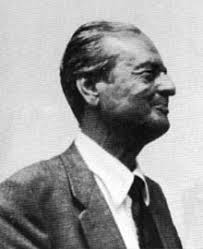
\includegraphics[width=0.9\columnwidth]{finetti.jpg}
        \end{column}
    \end{columns}
\end{frame}

\begin{frame}{PROBABILIDADE NÃO EXISTE!\footnote{\textcite{definettiTheoryProbability1974}}}
    \begin{columns}
        \begin{column}{0.6\textwidth}
            \begin{vfilleditems}
                \small
                \item Considere jogar uma moeda de enviesada
                \item As tentativas são consideradas independentes e, como resultado,
                      exibem outra propriedade importante: \textbf{a ordem não importa}
                \item A frequência é considerada uma \textbf{estatística suficiente}
                \item Dizer que a ordem não importa ou dizer que a única coisa que
                      importa é a frequência são duas maneiras de dizer exatamente a
                      mesma coisa
                \item Dizemos que essa probabilidade é \textbf{invariante sob permutações}
            \end{vfilleditems}
        \end{column}
        \begin{column}{0.4\textwidth}
            \begin{tikzpicture}[
                scale=0.55,
                transform shape, thick,
                every node/.style = {draw, circle, minimum size = 10mm},
                grow = down,  % alignment of characters
                level 1/.style = {sibling distance=3cm},
                level 2/.style = {sibling distance=1.5cm},
                level 3/.style = {sibling distance=3cm},
                level distance = 3cm,
                head/.style = {fill = orange!90!blue,
                label = center:\textsf{\Large C}},
                tail/.style = {fill = blue!70!yellow, text = black,
                label = center:\textsf{\Large K}}
                ]
                \node[shape = circle split, draw, line width = 1pt,
                      minimum size = 10mm, inner sep = 0mm, font = \sffamily\large,
                      rotate=30] (Start)
                      { \rotatebox{-30}{H} \nodepart{lower} \rotatebox{-30}{T}}
                child {   node [head] (A) {}
                    child { node [head] (B) {}}
                    child { node [tail] (C) {}}
                }
                child {   node [tail] (D) {}
                    child { node [head] (E) {}}
                    child { node [tail] (F) {}}
                };

              % Filling the root (Start)
              \begin{scope}[on background layer, rotate=30]
                \fill[head] (Start.base) ([xshift = 0mm]Start.east) arc (0:180:5mm)
                  -- cycle;
                \fill[tail] (Start.base) ([xshift = 0pt]Start.west) arc (180:360:5mm)
                  -- cycle;
              \end{scope}

              % Labels
              \begin{scope}[nodes = {draw = none}]
                \path (Start) -- (A) node [near start, left]  {$0.5$};
                \path (A)     -- (B) node [near start, left]  {$0.5$};
                \path (A)     -- (C) node [near start, right] {$0.5$};
                \path (Start) -- (D) node [near start, right] {$0.5$};
                \path (D)     -- (E) node [near start, left]  {$0.5$};
                \path (D)     -- (F) node [near start, right] {$0.5$};
                \begin{scope}[nodes = {below = 11pt}]
                  \node at (B) {$0.25$};
                  \node at (C) {$0.25$};
                  \node at (E) {$0.25$};
                  \node at (F) {$0.25$};
                \end{scope}
              \end{scope}
            \end{tikzpicture}
        \end{column}
    \end{columns}
\end{frame}

\begin{frame}{Interpretações da Probabilidade}
    \begin{vfilleditems}
        \item \textbf{Objetiva} - frequência no longo prazo de um evento específico
        \begin{vfilleditems}
            \item $P(\text{chuva}) = \frac{\text{dias que choveram}}{\text{dias totais}}$
            \item $P(\text{chance de eu ser presidente} = 0)$ (Nunca ocorreu)
        \end{vfilleditems}
        \item \textbf{Subjetiva} - nível de crença em um evento
        \begin{vfilleditems}
            \item $P(\text{chuva}) = \text{crença que choverá}$
            \item $P(\text{chance de eu ser presidente} = 10^{-10})$ (Muito improvável)
        \end{vfilleditems}
    \end{vfilleditems}
\end{frame}

\subsubsection{O que é Probabilidade?}
\begin{frame}{O que é Probabilidade?}
    \begin{defn}[Probabilidade]
    Sobre notação, definimos que $A$ é um evento e $P(A)$ a probabilidade do evento, logo:
    $$
    \{P(A) \in \mathbb{R} : 0 \leq P(A) \leq 1 \}.
    $$
    \vfill
    Isto quer dizer o "probabilidade do evento $A$ ocorrer é o conjunto de
    todos os números reais entre $0$ e $1$; incluindo $0$ e $1$"
    \end{defn}
\end{frame}

\begin{frame}{Axiomas da Probabilidade\footnote{\textcite{kolmogorovFoundationsTheoryProbability1933}}}
    \begin{columns}
        \begin{column}{0.8\textwidth}
        \begin{vfilleditems}
            \item \textbf{Não-negatividade}: Para todo $A$, $P(A) \geq 0$.
            Toda probabilidade é positiva (maior ou igual a zero), independente do
            evento
            \item \textbf{Aditividade}: Para dois \textit{mutuamente exclusivos}
            $A$ e $B$ (não podem ocorrer ao mesmo tempo):
            $P(A) = 1 - P(B)$ e $P(B) = 1 - P(A)$
            \item \textbf{Normalização}: A probabilidade de todos os eventos
            possíveis $A_1, A_2, \dots$ devem somar $1$:
            $\sum_{n \in \mathbb{N}} A_n = 1$
        \end{vfilleditems}
        \end{column}
        \begin{column}{0.2\textwidth}
        \centering
        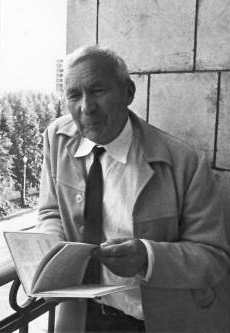
\includegraphics[width=0.9\columnwidth]{kolmogorov.jpg}
        \end{column}
    \end{columns}
\end{frame}

\begin{frame}{Espaços Amostrais}
    \begin{vfilleditems}
        \item Discretos $$\Theta = \left\{1, 2, \ldots, \right\}$$
        \item Contínuos $$\Theta \in \left(-\infty, \infty \right)$$
    \end{vfilleditems}
\end{frame}

\begin{frame}{Espaços Amostrais Discretos}
    8 Planetas do Nosso Sistema Solar
    \begin{vfilleditems}
        \item Mercúrio - $\mercury$
        \item Vênus - $\venus$
        \item Terra - $\earth$
        \item Marte $\mars$
        \item Júpiter - $\jupiter$
        \item Saturno $\saturn$
        \item Urano - $\uranus$
        \item Netuno $\neptune$
    \end{vfilleditems}
\end{frame}

\begin{frame}[fragile]{Espaços Amostrais Discretos\footnote{figuras adaptadas de \href{https://github.com/betanalpha/stan_intro}{Michael Betancourt (CC-BY-SA-4.0)}}}
\footnotesize
\begin{figure}
\centering
\subfigure{
\begin{tikzpicture}[scale=0.25, thick]
  \draw[color=black] (-25, 0) to (10, 0);
  \node[] at (-15, 0) {O planeta possui campo magnético};
  \node[] at (7, 2) {$\theta \in E_{1}$};

  \fill[color=gray60] (0, 0) circle (25pt) node[color=black] {$\mercury$};
  \fill[color=blue] (2, 0) circle (25pt) node[color=black] {$\venus$};
  \fill[color=blue] (4, 0) circle (25pt) node[color=black] {$\earth$};
  \fill[color=gray60] (6, 0) circle (25pt) node[color=black] {$\mars$};
  \fill[color=blue] (8, 0) circle (25pt) node[color=black] {$\jupiter$};
  \fill[color=blue] (10, 0) circle (25pt) node[color=black] {$\saturn$};
  \fill[color=blue] (12, 0) circle (25pt) node[color=black] {$\uranus$};
  \fill[color=blue] (14, 0) circle (25pt) node[color=black] {$\neptune$};
  \end{tikzpicture}
}
%
\subfigure{
\begin{tikzpicture}[scale=0.25, thick]
  \draw[color=black] (-25, 0) to (10, 0);
  \node[] at (-15, 0) {O planeta possui luas};
  \node[] at (7, 2) {$\theta \in E_{2}$};

  \fill[color=gray60] (0, 0) circle (25pt) node[color=black] {$\mercury$};
  \fill[color=gray60] (2, 0) circle (25pt) node[color=black] {$\venus$};
  \fill[color=blue] (4, 0) circle (25pt) node[color=black] {$\earth$};
  \fill[color=blue] (6, 0) circle (25pt) node[color=black] {$\mars$};
  \fill[color=blue] (8, 0) circle (25pt) node[color=black] {$\jupiter$};
  \fill[color=blue] (10, 0) circle (25pt) node[color=black] {$\saturn$};
  \fill[color=blue] (12, 0) circle (25pt) node[color=black] {$\uranus$};
  \fill[color=blue] (14, 0) circle (25pt) node[color=black] {$\neptune$};
\end{tikzpicture}
}
%
\subfigure{
\begin{tikzpicture}[scale=0.25, thick]
  \draw[color=black] (-25, 0) to (10, 0);
  \node[] at (-15, 0) {O planeta possui campo magnético e luas};
  \node[] at (7, 2) {$\theta \in E_{1} \cap E_{2}$};

  \fill[color=gray60] (0, 0) circle (25pt) node[color=black] {$\mercury$};
  \fill[color=gray60] (2, 0) circle (25pt) node[color=black] {$\venus$};
  \fill[color=blue] (4, 0) circle (25pt) node[color=black] {$\earth$};
  \fill[color=gray60] (6, 0) circle (25pt) node[color=black] {$\mars$};
  \fill[color=blue] (8, 0) circle (25pt) node[color=black] {$\jupiter$};
  \fill[color=blue] (10, 0) circle (25pt) node[color=black] {$\saturn$};
  \fill[color=blue] (12, 0) circle (25pt) node[color=black] {$\uranus$};
  \fill[color=blue] (14, 0) circle (25pt) node[color=black] {$\neptune$};
\end{tikzpicture}
}
%
\subfigure{
\begin{tikzpicture}[scale=0.25, thick]
  \node[] at (-15, 0) {O planeta possui campo magnético ou luas};
  \node[] at (7, 2) {$\theta \in E_{1} \cup E_{2}$};

  \fill[color=gray60] (0, 0) circle (25pt) node[color=black] {$\mercury$};
  \fill[color=blue] (2, 0) circle (25pt) node[color=black] {$\venus$};
  \fill[color=blue] (4, 0) circle (25pt) node[color=black] {$\earth$};
  \fill[color=blue] (6, 0) circle (25pt) node[color=black] {$\mars$};
  \fill[color=blue] (8, 0) circle (25pt) node[color=black] {$\jupiter$};
  \fill[color=blue] (10, 0) circle (25pt) node[color=black] {$\saturn$};
  \fill[color=blue] (12, 0) circle (25pt) node[color=black] {$\uranus$};
  \fill[color=blue] (14, 0) circle (25pt) node[color=black] {$\neptune$};
\end{tikzpicture}
}
%
\subfigure{
\begin{tikzpicture}[scale=0.25, thick]
  \node[] at (-15, 0) {O planeta não possui um campo magnético};
  \node[] at (7, 2) {$\theta \in \neg E_{1}$};

  \fill[color=blue] (0, 0) circle (25pt) node[color=black] {$\mercury$};
  \fill[color=gray60] (2, 0) circle (25pt) node[color=black] {$\venus$};
  \fill[color=gray60] (4, 0) circle (25pt) node[color=black] {$\earth$};
  \fill[color=blue] (6, 0) circle (25pt) node[color=black] {$\mars$};
  \fill[color=gray60] (8, 0) circle (25pt) node[color=black] {$\jupiter$};
  \fill[color=gray60] (10, 0) circle (25pt) node[color=black] {$\saturn$};
  \fill[color=gray60] (12, 0) circle (25pt) node[color=black] {$\uranus$};
  \fill[color=gray60] (14, 0) circle (25pt) node[color=black] {$\neptune$};
\end{tikzpicture}
}
%
\end{figure}
\end{frame}

\begin{frame}{Espaços Amostrais Contínuos\footnote{figuras adaptadas de \href{https://github.com/betanalpha/stan_intro}{Michael Betancourt (CC-BY-SA-4.0)}}}
\footnotesize
\begin{figure}
\centering
\subfigure{
\begin{tikzpicture}[scale=0.25, thick]
  \draw[color=black] (-27, 0) to (17, 0);
  \node[align=center] at (-15, 0) {A distância é menos que cinco centímetros};
  \node[] at (7.5, 2) {$\theta \in E_{1}$};

  \draw[|->] (0, 0) -- (14,0) node[right] {$x$};
  \draw[line width=1mm, color=blue] (0, 0) node[] {$\,($} -- (5, 0) node[] {$\!)$};
\end{tikzpicture}
}
%
\subfigure{
\begin{tikzpicture}[scale=0.25, thick]
  \draw[color=black] (-27, 0) to (17, 0);
  \node[align=center] at (-15, 0) {A distância é entre três e sete centímetros};
  \node[] at (7.5, 2) {$\theta \in E_{2}$};

  \draw[|->] (0, 0) -- (14,0) node[right] {$x$};
  \draw[line width=1mm, color=blue] (3, 0) node[] {$\,($} -- (7,0) node[] {$\!)$};

\end{tikzpicture}
}
%
\subfigure{
\begin{tikzpicture}[scale=0.25, thick]
  \draw[color=black] (-27, 0) to (17, 0);
  \node[align=center] at (-15, 0) {A distância é menos que cinco centímetros \\ e entre três e sete centímetros};
  \node[] at (7.5, 2) {$\theta \in E_{1} \cap E_{2}$};

  \draw[|->] (0, 0) -- (14,0) node[right] {$x$};
  \draw[line width=1mm, color=blue] (3, 0) node[] {$\,($} -- (5, 0) node[] {$\!)$};
\end{tikzpicture}
}
%
\subfigure{
\begin{tikzpicture}[scale=0.25, thick]
  \draw[color=black] (-27, 0) to (17, 0);
  \node[align=center] at (-15, 0) {A distância é menos que cinco centímetros \\ ou entre três e sete centímetros};
  \node[] at (7.5, 2) {$\theta \in E_{1} \cup E_{2}$};

  \draw[|->] (0, 0) -- (14, 0) node[right] {$x$};
  \draw[line width=1mm, color=blue] (0, 0) node[] {$\,($} -- (7, 0) node[] {$\!)$};
\end{tikzpicture}
}
%
\subfigure{
\begin{tikzpicture}[scale=0.25, thick]
  \draw[color=black] (-27, 0) to (17, 0);
  \node[align=center] at (-15, 0) {A distância não é menos que cinco centímetros};
  \node[] at (7.5, 2) {$\theta \in \neg E_{1}$};

  \draw[|->] (0, 0) -- (14, 0) node[right] {$x$};
  \draw[line width=1mm, color=blue] (5, 0) node[] {$\,($} -- (13, 0);
\end{tikzpicture}
}
\end{figure}
\end{frame}

\begin{frame}{Parâmetros Discretos versus Contínuos}

    Tudo o que foi exposto até agora partiu do pressuposto que os parâmetros
    são discretos. Isto foi feito com o intuito de prover uma melhor intuição
    do que é probabilidade. Nem sempre trabalhamos com parâmetros discretos.
    Os parâmetros podem ser contínuos, como por exemplo: idade, altura, peso etc.
    Mas não se desespere, todas as regras e axiomas da probabilidade são válidos
    também para parâmetros contínuos. A única coisa que temos que fazer é trocar
    todas as somas $\sum$ por integrais $\int$. Por exemplo o terceiro axioma de
    \textbf{Normalização} para variáveis aleatórias contínuas se torna:

    $$
    \int_{x \in X} p(x) dx = 1.
    $$

\end{frame}


\begin{frame}{Probabilidade Condicional}
    \begin{defn}[Probabilidade Condicional]
        Probabilidade de um evento ocorrer caso outro tenha ocorrido ou não. \newline \newline
        A notação que usamos é $P( A \mid B )$, que lê-se como "a probabilidade
        de observamos $A$ dado que já observamos $B$". \newline \newline
    \vfill \vfill
    $$
            \begin{aligned}
                P(A \mid B) &= \frac{\text{número de elementos em $A$ e $B$}}{\text{número de elemementos em $B$}} \\
                P(A \mid B) &= \frac{P(A \cap B)}{(B)}
        \end{aligned}
    $$
        \newline \newline \hspace{0.7\textwidth}
        {\footnotesize assumimos que $P(B) > 0$}.
    \end{defn}
\end{frame}

\begin{frame}{Exemplo de Probabilidade Condicional}
    \begin{exemplo}[Poker Texas Hold'em]
        \begin{vfilleditems}
            \item \textbf{Espaço Amostral}: $52$ cartas no baralho, $13$ tipos de cartas e $4$ tipos de naipes.
            \item $P(A)$: Chance de receber um Ás $\left( \frac{4}{52} = \frac{1}{13}\right)$
            \item $P(K)$: Chance de receber um Rei (K) $\left( \frac{4}{52} = \frac{1}{13} \right)$
            \item $P(A \mid K)$: Chance de receber um Ás, dado que você recebeu um Rei (K) $\left( \frac{4}{51} \approx 0.078 \right)$
            \item $P(K \mid A)$: Chance de receber um Rei (K), dado que você recebeu um Ás $\left( \frac{4}{51} \approx 0.078 \right)$
        \end{vfilleditems}
    \end{exemplo}
\end{frame}

\begin{frame}{Cuidado! Nem sempre $P(A \mid B) = P(B \mid A)$}
    No exemplo anterior temos a simetria $P(A \mid K) = P(K \mid A)$, \textbf{mas nem sempre isso é verdade}\footnote{Mais especificamente, se as taxas basais $P(A)$ e $P(B)$ não são iguais, a simetria é quebrada $P(A \mid B) \neq P(B \mid A)$!}
    \begin{exemplo}[O Papa é católico]
        \begin{vfilleditems}
            \small{
            \item $P(\text{papa})$: Chance alguém aleatório ser papa, algo bem pequeno, 1 em 8 bilhões $\left( \frac{1}{8 \cdot 10^9} \right)$
            \item $P(\text{católico})$: Chance alguém aleatório ser católico, 1.34 de 8 bilhões $\left( \frac{1.34}{8} \approx 0.17 \right)$
            \item $P(\text{católico} \mid \text{papa})$: Chance do Papa ser católico $\left( \frac{999}{1000} = 0.999 \right)$
            \item $P(\text{papa} \mid \text{católico})$: Chance de alguém católico ser o papa $\left( \frac{1}{1.34 \cdot 10^9} \cdot 0.999 \approx 7.46 \cdot 10^{-10} \right)$
            }
            \item \large{\textbf{Logo}: $P(\text{católico} \mid \text{papa}) \neq P(\text{papa} \mid \text{católico})$}
        \end{vfilleditems}
    \end{exemplo}
\end{frame}

\begin{frame}{Um clássico da Probabilidade}
    \begin{columns}
        \begin{column}{0.6\textwidth}
            \begin{exemplo}[Monty Hall]
            \begin{vfilleditems}
                \small
                \item Um apresentador de TV lhe apresenta 3 portas
                \item Uma delas tem um prêmio: um carro! As outras tem um bode
                \item Você deve escolher uma porta (que não é aberta)
                \item Nesse momento Monty abre uma das outras duas portas que você
                não escolheu, revelando que o carro não se encontra nessa porta e revelando um dos bodes
                \item Monty então lhe pergunta "Você quer manter sua escolha de porta ou trocar?"
            \end{vfilleditems}
        \end{exemplo}
        \end{column}
        \begin{column}{0.4\textwidth}
            \begin{figure}
                \centering
                \def\svgwidth{\columnwidth}
                \input{../images/monty_hall.pdf_tex}
            \end{figure}
        \end{column}
    \end{columns}
\end{frame}

\begin{frame}{Solução do Problema de Monty Hall}
    \begin{idea}[Probabilidade de ganhar o carro]
    $$
        \begin{aligned}
    P(\text{carro} \mid C_i) &= \frac{1}{3} \\
    P(\text{carro}) &= \frac{1}{3} \cdot P(\text{carro} \mid C_1) + \frac{1}{3} \cdot P(\text{carro} \mid C_2) + \frac{1}{3} \cdot P(\text{carro} \mid C_3) \\
    P(\text{carro}) &= \frac{\sum^3_{i=1}P(\text{carro} \mid C_i)}{3} \\
    P(\text{carro}) &= \frac{1}{3}
    \end{aligned}
    $$
    \end{idea}
    \vfill \vfill
    $C_i$ é o evento no qual o carro está atrás da porta $i$, $i=1,2,3$
\end{frame}

\begin{frame}[t]{Solução do Problema de Monty Hall\footnote{se você não acredita nesse resultado veja como simular o problema de Monty Hall nos \hyperlink{appendixmontyhall}{Slides de Backup no final dessa apresentação}}}
    \begin{columns}[t]
        \begin{column}{0.5\textwidth}
            {\Large \textbf{Cenário 1}: Não trocar de porta} \newline \newline
            Simples: $$\frac{1}{3}$$
        \end{column}
        \begin{column}{0.5\textwidth}
            {\Large \textbf{Cenário 2}: Trocar de porta} \newline \newline
            Escolha qualquer porta $i$ para ser $C_i = 0$
            \vfill
            $$
            \begin{aligned}
                P(\text{carro}) &= 0 \cdot P(\text{carro} \mid C_i) + \frac{1}{3} + \frac{1}{3} \\
                P(\text{carro}) &= \frac{2}{3}
            \end{aligned}
            $$
        \end{column}
    \end{columns}
\end{frame}

\begin{frame}{Visualização do Problema de Monty Hall}
\begin{figure}
\centering
\subfigure{
    \begin{tikzpicture}[
        scale=0.55,
        header/.style = {draw, rectangle, fill = blue!50!black, minimum size = 10mm},
        level distance = 3.5cm,
        transform shape, thick,
        grow = right, sloped,
        ]
        \node[header] {Sua Escolha}
            child{
                node[header] {Carro está}
                edge from parent[draw=none]
                child{
                    node[header] {Monty abre}
                    edge from parent[draw=none]
                    child{
                        node[header] {resultado}
                        edge from parent[draw=none]
                    }
                }
            };
    \end{tikzpicture}
}
%
\subfigure{
    \begin{tikzpicture}[
        scale=0.55,
        door/.style = {draw, circle, minimum size = 10mm},
        car/.style = {circle, fill = green!50!black, minimum size = 10mm},
        goat/.style = {circle, fill = red!50!black, minimum size = 10mm},
        level distance = 3.5cm,
        transform shape, thick,
        grow = right, sloped,
        level 1/.style = {sibling distance=3.5cm},
        level 2/.style = {sibling distance=2cm},
        level 3/.style = {sibling distance=3cm}
        ]
    \node[door] {Porta 1}
        child {
        node[door] {Porta 3}
            child {
                node[door] {Porta 2}
                child {
                    node[car, label=right:{\Large$\frac{1}{3}$}] {Carro}
                }
                edge from parent
                node[above] {\Large$1$}
            }
            edge from parent
            node[below] {\Large$\frac{1}{3}$}
        }
        child {
        node[door] {Porta 2}
            child {
                node[door] {Porta 3}
                child {
                    node[car, label=right:{\Large$\frac{1}{3}$}] {Carro}
                }
                edge from parent
                node[above] {\Large$1$}
            }
            edge from parent
            node[above] {\Large$\frac{1}{3}$}
        }
        child {
            node[door] {Porta 1}
            child {
                node[door] {Porta 2}
                    child {
                        node[goat, label=right:{\Large$\frac{1}{6}$}] {Bode}
                    }
                    edge from parent
                    node[above]  {\Large$\frac{1}{2}$}
                }
                child {
                    node[door] {Porta 3}
                    child {
                        node[goat, label=right:{\Large$\frac{1}{6}$}] {Bode}
                    }
                    edge from parent
                    node[above]  {\Large$\frac{1}{2}$}
                }
            edge from parent
            node[above] {\Large$\frac{1}{3}$}
        };
    \end{tikzpicture}
}
\end{figure}
\end{frame}

\begin{frame}{Probabilidade Conjunta}
    \begin{defn}[Probabilidade Conjunta]
        Probabilidade de observados dois ou mais eventos ocorrem. \newline \newline
        A notação que usamos é $P(A, B)$, que lê-se como
        "a probabilidade de observamos $A$ e também observamos $B$". \newline \newline
        $$
            \begin{aligned}
                P(A,B) &= \text{número de elementos em $A$ ou $B$} \\
                P(A,B) &= P(A \cup B)
            \end{aligned}
        $$
    \end{defn}
\end{frame}

\begin{frame}{Exemplo de Probabilidade Conjunta}
    \begin{exemplo}[Revisitando Poker Texas Hold'em]
        \begin{vfilleditems}
            {\footnotesize
            \item \textbf{Espaço Amostral}: $52$ cartas no baralho, $13$ tipos de cartas e $4$ tipos de naipes.
            \item $P(A)$: Chance de receber um Ás $\left( \frac{4}{52} = \frac{1}{13}\right)$
            \item $P(K)$: Chance de receber um Rei (K) $\left( \frac{4}{52} = \frac{1}{13} \right)$
            \item $P(A \mid K)$: Chance de receber um Ás, dado que você recebeu um Rei (K) $\left( \frac{4}{51} \approx 0.078 \right)$
            \item $P(K \mid A)$: Chance de receber um Rei (K), dado que você recebeu um Ás $\left( \frac{4}{51} \approx 0.078 \right)$
            }
            \item $P(A, K)$: Chance de receber um Ás e um Rei (K)
            $$
                \begin{aligned}
                    P(A, K) &= P(K, A) \\
                    P(A) \cdot P(K \mid A) &= P(K) \cdot P(A \mid K) \\
                    \frac{1}{13} \cdot \frac{4}{51} &= \frac{1}{13} \cdot \frac{4}{51} \\
                    &\approx 0.006
                \end{aligned}
            $$
        \end{vfilleditems}
    \end{exemplo}
\end{frame}

% Exemplo do Poker com pacote pst-poker
% Exemplo do Papa e Católico

% Bivariate Normal inspirada aqui: https://github.com/walmes/Tikz/blob/master/src/bivariate-normal.pgf
\begin{frame}{Visualização de Probabilidade Conjunta vs Probabilidade Condicional}
    \centering
    \begin{tikzpicture}[scale=0.9]
      \begin{axis}[
      domain   = -3.5:3.5,
      domain y = -3.5:3.5,
      view = {-70}{20},
      title={$P(X,Y)$ versus $P(X \mid Y=-0.75)$},
      xlabel={$X$},
      ylabel={$Y$},
      % zlabel={$SSE(\beta_0, \beta_1)$},
      zmin = -0,
      %xticklabels=\empty,
      %yticklabels=\empty,
      zticklabels=\empty,
      xtick=\empty,
      ytick={-0.75},
      ztick=\empty,
      axis z line*=none,
      axis y line*=left,
      axis x line*= bottom]
       \addplot3 [
        domain = -3.5:3.5,
        samples = 50, samples y = 0,
        thick, smooth, color = red, fill = orange, opacity = 0.75]
        (x, -0.75, {conditionalbinormal(-0.75, 0, 1, 0, 1, 0.75)});

        \draw (-3.5, -0.75, 0) -- (3.5, -0.75, 0);

        \addplot3 [
          surf,
          domain = -3.5:3.5,
          samples = 50,
          opacity = 0.15,
          faceted color = colorB,
          colormap = {blueblack}{
            color = (colorB)
            color = (colorA!50!white)
            color = (colorA)}]
            {binormal(0, 1, 0, 1, 0.7)};
      \end{axis}
    \end{tikzpicture}
\end{frame}

% Countour plot inspirado daqui: https://tex.stackexchange.com/a/31713/200209
\begin{frame}{Visualização de Probabilidade Conjunta vs Probabilidade Condicional}
    \begin{columns}
    \begin{column}{0.5\textwidth}
    \centering
    \begin{tikzpicture}[scale=0.5]
        \begin{axis}[
            view={0}{90},
            axis equal,
            enlarge y limits=true,
            title={$P(X,Y)$},
            xlabel={$X$},
            ylabel={$Y$},
            xtick=\empty,
            ytick={-0.75}
            ]

            \draw[red, line width=2pt] (-3.5, -0.75) -- (3.5, -0.75);

            \addplot3[contour gnuplot={labels=false},domain=-3.5:3.5,domain y=-3.5:3.5]
                {exp(-( x^2 + y^2)/3 )};

        \end{axis}
    \end{tikzpicture}
    \end{column}
    \begin{column}{0.5\textwidth}
    \centering
    \begin{tikzpicture}[scale=0.5]
        \begin{axis}[every axis plot, line width=2pt,
            title={$P(X \mid Y=-0.75)$},
            xlabel={$X$},
            ylabel={$Y$},
            xtick=\empty,
            ytick=\empty,
            domain=-3.5:3.5,samples=200,
            axis x line*=bottom, % no box around the plot, only x and y axis
            axis y line*=left, % the * suppresses the arrow tips
            enlarge x limits=true
            ] % extend the axes a bit

            \addplot [red, fill = red, fill opacity = 0.5] {exp(-( x^2 + -0.75^2)/3 )};
        \end{axis}
    \end{tikzpicture}
    \end{column}
\end{columns}
\end{frame}

\subsubsection{Teorema de Bayes}
\begin{frame}{Quem foi Thomas Bayes?}
    \begin{columns}
        \begin{column}{0.8\textwidth}
            \begin{vfilleditems}
                \item \small Thomas Bayes (1701 - 1761) foi um estatístico, filósofo
                e ministro presbiteriano inglês conhecido por formular um caso
                específico do teorema que leva seu nome
                \item \small Bayes nunca publicou o que se tornaria sua realização mais famosa;
                suas notas foram editadas e publicadas após sua morte pelo seu amigo
                Richard Price
                \item \small O nome formal do teorema é Bayes-Price-Laplace, pois Thomas
                Bayes foi o primeiro a descobrir, Richard Price pegou seus rascunhos,
                formalizou em notação matemática e apresentou para a Royal Society of London,
                e Pierre Laplace redescobriu o teorema sem ter tido contato prévio no final
                do século XVIII na França ao usar probabilidade para inferência estatística
                com dados do Censo na era Napoleônica
            \end{vfilleditems}
        \end{column}
        \begin{column}{0.2\textwidth}
            \centering
            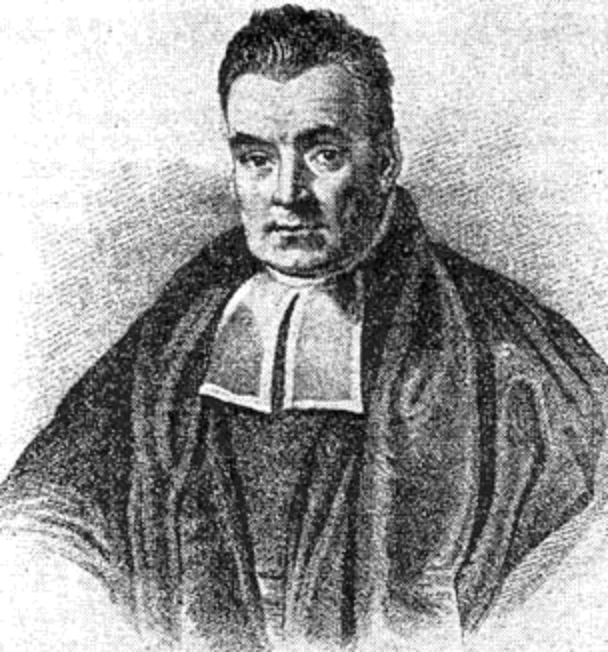
\includegraphics[width=0.9\columnwidth]{thomas_bayes.png}
        \end{column}
    \end{columns}
\end{frame}


\begin{frame}{Teorema de Bayes}
    \begin{theo}[Bayes]
        Nos diz como "inverter" a probabilidade condicional: \newline \newline
        $$P(A \mid B) = \frac{P(A) \cdot P(B \mid A)}{P(B)}$$
    \end{theo}
\end{frame}

\begin{frame}{Prova do Teorema de Bayes}
    Lembra que temos a seguinte identidade na probabilidade:
    $$
    \begin{aligned}
    P(A,B) &= P(B,A) \\
    P(A) \cdot P(B \mid A) &= P(B) \cdot P(A \mid B)
    \end{aligned}
    $$

    Pois bem, agora passe o $P(B)$ do lado direito para o lado esquerdo dividindo:
    $$
    \begin{aligned}
    P(A) \cdot P(B \mid A) &= \overbrace{P(B)}^{\text{isso vai para $\leftarrow$}} \cdot \quad P(A \mid B) \\
    &\\
    \frac{P(A) \cdot P(B \mid A)}{P(B)} &= P(A \mid B) \\
    P(A \mid B) &= \frac{P(A) \cdot P(B \mid A)}{P(B)}
    \end{aligned}
    $$
\end{frame}

\begin{frame}{Visualização do Teorema de Bayes}
    \begin{columns}
        \begin{column}{0.6\textwidth}
            \begin{tikzpicture}[thick]
                \node[circle, label={137:Espaço Amostral}, fill=red!20!white, fill opacity = 0.5, minimum size=6cm] (Omega) at (0,0) {};
                \node[ellipse, label={35:$E_1$}, fill=blue, fill opacity = 0.5, minimum width=5.5cm, minimum height=2cm] (Ellipse) at (0,1) {};
                \node[circle, label={178:$E_2$}, fill=red, fill opacity = 0.5, minimum size = 1cm] (Circulo) at (-1.5,1) {};
                \node[] (KK) at (-1.5, 1) {$KK$};
                \node[] (CC) at (1.5, 1) {$CC$};
                \node[] (KC) at (1.5, -1) {$KC$};
                \node[] (CK) at (-1.5, -1) {$CK$};
            \end{tikzpicture}
        \end{column}
        \begin{column}{0.4\textwidth}
            $$
            \begin{aligned}
                E_1 &= P(KK  \cup CC) \\
                E_2 &= P(KK \mid E_1)
            \end{aligned}
            $$
        \end{column}
    \end{columns}
\end{frame}

\begin{frame}{Mais um clássico da Probabilidade\footnote{Origem: \href{https://www.yudkowsky.net/rational/bayes}{Yudkowski - \textit{An Intuitive Explanation of Bayes’ Theorem}}}}
    \begin{exemplo}[Cancêr de Mama]
        \small
        O quão acurado é o teste de \textbf{câncer de mama}?
        \begin{vfilleditems}
            \item \footnotesize 1\% das mulheres têm \textbf{câncer de mama} (Prevalência)
            \item \footnotesize 80\% das mamografias detectam o \textbf{câncer de mama} (Verdadeiro Positivo)
            \item \footnotesize 9.6\% das mamografias detectam \textbf{câncer de mama} quando não há incidência (Falso Positivo)
        \end{vfilleditems}
        $$
        \begin{aligned}
            P(C \mid +) &= \frac{P(+ \mid C) \cdot P(C)}{P(+)} \\
            P(C \mid +) &= \frac{P(+ \mid C) \cdot P(C)}{P(+ \mid C) \cdot P(C) + P(+ \mid \neg C) \cdot P(\neg C)} \\
            P(C \mid +) &= \frac{0.8 \cdot 0.01}{0.8 \cdot 0.01 + 0.096 \cdot 0.99} \\
            P(C \mid +) &\approx 0.0776
        \end{aligned}
        $$
    \end{exemplo}
\end{frame}


\begin{frame}{Porquê o teorema de Bayes é Importante?}
    \begin{idea}[Podemos Inverter a Probabilidade Condicional]
        $$
        \begin{aligned}
            P(\text{hipótese} \mid \text{dados}) = \frac{P(\text{hipótese}) \cdot P(\text{dados} \mid \text{hipótese})}{P(\text{data})}
        \end{aligned}
        $$
    \end{idea}
    Mas isso não é o $p$-valor? \textcolor{red}{\textbf{NÃO!}}
\end{frame}

\subsection{Estatística Frequentista versus Bayesiana}
\subsubsection{O que são $p$-valores e Intervalos de Confiança}
\begin{frame}{O que é o $p$-valor?}
    \begin{defn}[$p$-valor]
        $p$-valor é a probabilidade de obter resultados no mínimo tão
        extremos quanto os que foram observados, dado que a hipótese nula
        $H_0$ é verdadeira
        $$P(D \mid H_0)$$
    \end{defn}
\end{frame}

\begin{frame}{O que \textbf{não é} o $p$-valor!}
    \centering
    
\includegraphics[width=0.7\textwidth]{meme-pvalue.jpg}
\end{frame}

\begin{frame}{O que \textbf{não é} o $p$-valor!}
    \begin{vfilleditems}
        \item \textbf{$p$-valor não é a probabilidade da Hipótese nula}
        - Famosa confusão entre $P(D \mid H_0)$ e $P(H_0 \mid D)$.
        Para obter a $P(H_0 \mid D)$ você precisa de estatística Bayesiana.
        \item \textbf{$p$-valor não é a probabilidade dos dados serem produzidos pelo acaso}
        - \textcolor{red}{Não!} Ninguém falou nada de acaso.
        \item \textbf{$p$-valor mensura o tamanho do efeito de um teste estatístico}
        - Também \textcolor{red}{não}... $p$-valor não diz nada sobre o tamanho do efeito.
        Apenas sobre se o quanto os dados observados divergem do esperado sob a hipótese nula.
        Além disso, $p$-valores podem ser "hackeados" de diversas maneiras \parencite{head2015extent}.
    \end{vfilleditems}
\end{frame}

\begin{frame}{A relação entre $p$-valor e $H_0$}
    Para descobrir o $p$-valor, \textbf{descubra a $H_0$ que está por trás dele}.
    Sua definição nunca mudará, pois ela sempre é $P(D \mid H_0)$:
    \begin{vfilleditems}
        \item \textbf{Teste $t$}: $P(D \mid \text{a diferença entre os grupos é zero})$
        \item \textbf{ANOVA}: $P(D \mid \text{não há diferença entre os grupos})$
        \item \textbf{Regressão}: $P(D \mid \text{coeficiente é nulo})$
        \item \textbf{Shapiro-Wilk}: $P(D \mid \text{população é distribuída como uma normal})$
    \end{vfilleditems}
\end{frame}

\begin{frame}{O que são Intervalos de Confiança?}
    \begin{columns}
        \begin{column}{0.8\textwidth}
            \begin{defn}[Intervalos de Confiança]
                \begin{quotation}
                    Um intervalo de confiança de X\% para um parâmetro é um intervalo
                    $(a, b)$ gerado por um procedimento que em amostragem repetida
                    tem uma probabilidade de X\% de conter o valor verdadeiro do
                    parâmetro, para todos os valores possíveis do parâmetro
                \end{quotation}
                \vfill \vfill
                \textcite{neyman1937outline} (o "pai" dos intervalos de confiança)
            \end{defn}
        \end{column}
        \begin{column}{0.2\textwidth}
            \centering
            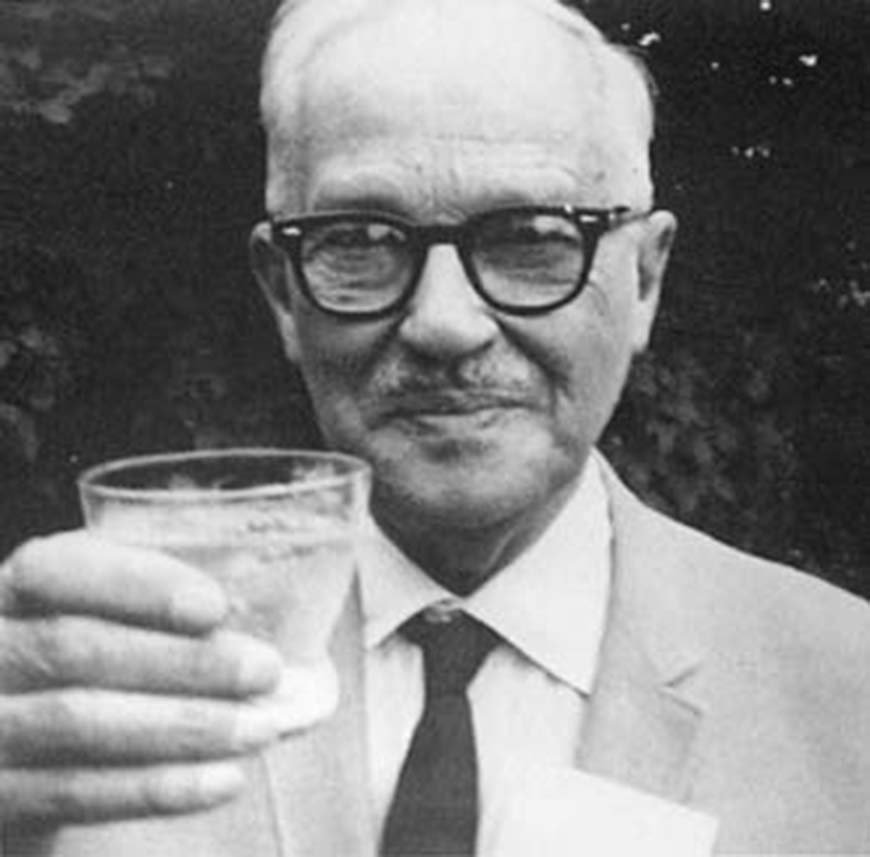
\includegraphics[width=0.9\columnwidth]{neyman.jpeg}
        \end{column}
    \end{columns}
\end{frame}

\begin{frame}{O que são Intervalos de Confiança?}
    \begin{exemplo}[Intervalo de Confiança de uma Política Pública]
        Digamos que você executou uma análise estatística para comparar
        eficácia de uma política pública em dois grupos e você obteve a
        diferença entre a média desses grupos. Você pode expressar essa
        diferença como um intervalo de confiança. Geralmente escolhemos a
        confiança de 95\%. Isso quer dizer que \textbf{95 estudos de 100},
        que usem o \textbf{mesmo tamanho de amostra e população-alvo},
        aplicando o \textbf{mesmo teste estatístico}, esperarão encontrar
        um resultado de diferenças de média entre grupos entre o intervalo
        de confiança.
    \end{exemplo}
    \footnotesize \textcolor{red}{Não diz nada sobre a sua \textbf{população-alvo},
    mas sim sobre a sua \textbf{amostra} num processo maluco de \textbf{amostragem infinita}...}
\end{frame}

\begin{frame}{Intevalos de Confiança versus Intervalos da Posterior}
    \centering
    \begin{tikzpicture}
        \begin{axis}[every axis plot, line width=2pt,
            xmin=0, xmax=4,
            ymin=0, ymax=1.5,
            ylabel=\empty,
            xlabel={$\theta$},
            samples=200,
            axis x line*=bottom, % no box around the plot, only x and y axis
            axis y line*=left,
            enlarge x limits=true,
            ] % extend the axes a bit

            \addplot [blue, domain=0:4, forget plot] {lognormal(0, 2)};
            \addplot+ [
                mark=none,
                area legend,
                line width=0pt,
                color=blue,
                fill=blue, fill opacity=0.5,
                domain=0.25950495026507125:3.8534910373715427
                ]
                {lognormal(0, 2)} \closedcycle;
            \addlegendentry{50\% Posterior}
            \addplot[red, mark=none] (-0.09, 1.4739034450607542) to (0.09, 1.4739034450607542);
            \addlegendentry{MLE}
            \draw [red] (0,0) to (0, 1.4739034450607542);
        \end{axis}
    \end{tikzpicture}
\end{frame}

\begin{frame}{Intevalos de Confiança versus Intervalos da Posterior}
    \centering
    \begin{tikzpicture}
        \begin{axis}[every axis plot, line width=2pt,
            xmin=-3, xmax=14,
            %ymin=0, ymax=1.5,
            ylabel=\empty,
            xlabel={$\theta$},
            samples=200,
            axis x line*=bottom, % no box around the plot, only x and y axis
            axis y line*=left,
            enlarge x limits=true,
            %legend pos=outer north east, %there is one default value for the `legend pos' that is outside the axis
            %legend cell align=left, % so the legend looks a bit better
            ] % extend the axes a bit

            \addplot [blue, domain=-3:14, forget plot] {sumtwonormals(2, 1, 0.6, 10, 1, 0.4)};
            \addplot+ [
                mark=none,
                area legend,
                line width=0pt,
                color=blue,
                fill=blue, fill opacity=0.5,
                domain=1.8:9.7
                ]
                {sumtwonormals(2, 1, 0.6, 10, 1, 0.4)} \closedcycle;
            \addlegendentry{50\% Posterior}
            \addplot[red, mark=none] (1.5, 0.24) to (2.5, 0.24);
            \addlegendentry{MLE}
            \draw [red] (2,0) to (2, 0.24);
        \end{axis}
    \end{tikzpicture}
\end{frame}

\begin{frame}{Mas por quê eu nunca vejo estatística sem $p$-valor?}
    \begin{columns}
        \begin{column}{0.8\textwidth}
            Não tem como entendermos $p$-valores se não compreendermos as suas
            origens e trajetória histórica. A primeira menção do termo foi feita
            pelo estatístico Ronald Fisher em 1925 \parencite{fisher1925statistical}:
            \begin{quotation}
                [$p$-valor é] índice que mede a força da evidência contra a hipótese nula
            \end{quotation}
            \begin{vfilleditems}
                \item Para quantificar a força da evidência contra a hipótese nula, Fisher defendeu
                "$p<0.05$ como um nível padrão para concluir que há evidência contra a hipótese testada"
                \item "Não seremos frequentemente perdidos se traçarmos uma linha convencional de 0.05"
            \end{vfilleditems}
        \end{column}
        \begin{column}{0.2\textwidth}
            \centering
            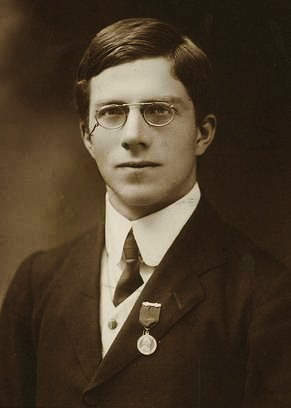
\includegraphics[width=0.9\columnwidth]{fisher.jpg}
        \end{column}
    \end{columns}
\end{frame}

\begin{frame}{$p = 0.06$}
    \begin{vfilleditems}
        \item Como o $p$-valor é uma probabilidade, ele é uma quantidade contínua.
        \item Não há razão para diferenciarmos um $p$ de 0.049 contra um $p$ de 0.051.
        \item Robert Rosenthal, um psicólogo já dizia "Deus ama $p$ de 0.06 tanto quanto um $p$ de 0.05"~\parencite{rosnow1989statistical}.
    \end{vfilleditems}
\end{frame}

\begin{frame}{Mas por quê eu nunca ouvi falar de Estatística Bayesiana?\footnote{\textit{inverse probability} é como o teorema de Bayes era chamado no começo do século XX}}
    \begin{columns}
        \begin{column}{0.8\textwidth}
            \begin{quotation}
                … it will be sufficient … to reaffirm my personal conviction …
                that the theory of inverse probability is founded upon an error,
                and must be wholly rejected.
            \end{quotation}
            \vfill \vfill
            \textcite{fisher1925statistical}
        \end{column}
        \begin{column}{0.2\textwidth}
            \centering
            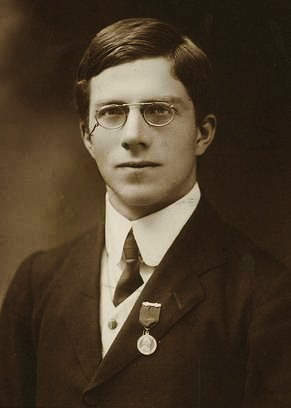
\includegraphics[width=0.9\columnwidth]{fisher.jpg}
        \end{column}
    \end{columns}
\end{frame}

\begin{frame}{Dentro de todo não Bayesiano há um Bayesiano querendo sair\footnote{Dennis Lindley "Inside every nonBayesian there is a Bayesian struggling to get out"}}
    \begin{columns}
        \begin{column}{0.8\textwidth}
            \begin{vfilleditems}
                \item No último ano de sua vida, Fisher publicou um artigo \parencite{fisherExamplesBayesMethod1962} examinando as possibilidades dos métodos Bayesianos, mas com as probabilidades a \textit{priori} a serem determinadas experimentalmente.
                \item Inclusive alguns autores especulam \parencite{jaynesProbabilityTheoryLogic2003} que se Fisher estivesse vivo hoje, ele provavelmente seria um "Bayesiano".
            \end{vfilleditems}
        \end{column}
        \begin{column}{0.2\textwidth}
            \centering
            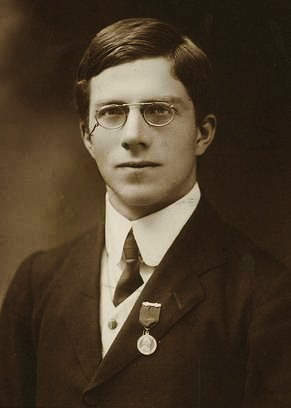
\includegraphics[width=0.9\columnwidth]{fisher.jpg}
        \end{column}
    \end{columns}
\end{frame}

\subsection{Estatística Bayesiana}
\begin{frame}{Teorema de Bayes como Motor de Inferência}
    \footnotesize Agora que você já sabe o que é probabilidade e o que é o teorema de Bayes, vou propor o seguinte modelo:
    $$
    \underbrace{P(\theta \mid y)}_{\text{Posterior}} = \frac{\overbrace{P(y \mid  \theta)}^{\text{Verossimilhança}} \cdot \overbrace{P(\theta)}^{\textit{Priori}}}{\underbrace{P(y)}_{\text{Constante Normalizadora}}}
    $$
    \begin{vfilleditems}
        \item \footnotesize $\theta$ -- parâmetro(s) de interesse
        \item \footnotesize $y$ -- dados observados
        \item \footnotesize \textbf{\textit{Priori}}: probabilidade prévia do valor do(s) parâmetro(s)
        \item \footnotesize \textbf{Verossimilhança}: probabilidade dos dados observados condicionados aos valores do(s) parâmetro(s)
        \item \footnotesize \textbf{Posterior}: probabilidade posterior do valor do(s) parâmetros após observamos os dados $y$
        \item \footnotesize \textbf{Constante Normalizadora}: $P(y)$ não faz sentido intuitivo. Essa probabilidade é transformada e pode ser interepretada como algo que existe apenas para que o resultado de $P(y \mid \theta) P(\theta)$ seja algo entre 0 e 1 -- uma probabilidade válida.
    \end{vfilleditems}
\end{frame}

\begin{frame}{Teorema de Bayes como Motor de Inferência}
    A estatísica Bayesiana nos permite \textbf{quantificar diretamente a incerteza}
    relacionada ao valor de um ou mais parâmetros do nosso modelo condicionado aos
    dados observados. Isso é a \textbf{característica principal} da estatística
    Bayesiana. Pois estamos estimando diretamente $P(\theta \mid y)$ por meio do
    teorema de Bayes. A estimativa resultante é totalmente intuitiva:
    simplesmente quantifica a intercerteza que temos sobre o valor de um ou mais
    parâmetro condicionado nos dados, nos pressupostos do nosso modelo
    (verossimilhança) e na probabilidade prévia que temos sobre tais valores.
\end{frame}

\subsubsection{Vantagens da Estatísca Bayesiana}
\begin{frame}{Estatística Bayesiana vs Frequentista}
    %\begin{table}[h!]
        \small
        \begin{tabular}{|l|p{.3\textwidth}|p{.3\textwidth}|}
        \toprule
                                & \textcolor{blue}{\textbf{Estatística Bayesiana}} & \textcolor{red}{\textbf{Estatística Frequentista}}                   \\ \midrule
        \textbf{Dados}          & Fixos –- Não Aleatórios                          & Incertos –- Aleatórios                                               \\ \midrule
        \textbf{Parâmetros}     & Incertos –- Aleatórios                           & Fixos –- Não Aleatórios                                              \\ \midrule
        \textbf{Inferência}     & Incerteza sobre o valor do parâmetro             & Incerteza sobre um processo de amostragem de uma população infinita  \\ \midrule
        \textbf{Probabilidade}  & Subjetiva                                        & Objetiva (mas com diversos pressupostos dos modelos)                 \\ \midrule
        \textbf{Incerteza}      & Intervalo de Credibilidade –- $P(\theta \mid y)$ & Intervalo de Confiança –- $P(y \mid \theta)$                         \\
        \bottomrule
        \end{tabular}
       %\end{table}
\end{frame}

\begin{frame}{Vantagens da Estatística Bayesiana}
    \begin{vfilleditems}
        \item Abordagem Natural para expressar Incerteza
        \item Habilidade de incorporar Informações Prévias
        \item Maior Flexibilidade do Modelo
        \item Distribuição Posterior completa dos Parâmetros
        \item Propagação Natural da Incerteza
    \end{vfilleditems}
    \small \textbf{Principal Desvantagem}: Velocidade lenta de estimativa de modelos\footnote{\textit{e.g.} 30 segundos ao invés de 3 segundos na abordagem frequentista}
\end{frame}

\begin{frame}{O começo do fim da Estatística Frequentista}
    \begin{vfilleditems}
        \small
        \item Saiba que você está em um momento da história no qual a Estatística está passando por grandes mudanças
        \item Acredito que a estatística frequentista, em especial a maneira que qualificamos evidências e hipóteses
        com $p$-valores se transformará de maneira "significante".
        \item Há cinco anos atrás, a \textit{American Statistical Association} (ASA) publicou uma declaração sobre
        $p$-valores \parencite{Wasserstein2016}. A declaração diz exatamente o que falamos aqui: Os conceitos principais do teste de significância de hipótese nula e, em particular $p$-valores não conseguem prover o que os pesquisadores requerem deles. Apesar do que dizem muitos livros de estatística, materiais de ensinos e artigos publicados, $p$-valores abaixo de 0,05 não "provam" a realidade de nada. Nem, chegando a esse ponto, os $p$-valores acima de 0,05 refutam alguma coisa.
        \item A declaração da ASA tem mais de 3.600 citações provocando impacto relevante.
    \end{vfilleditems}
\end{frame}

\begin{frame}{O começo do fim da Estatística Frequentista}
    \begin{vfilleditems}
        \small
        \item Um simpósio internacional foi promovido em 2017 que originou uma edição especial de acesso aberto da
        \textit{The American Statistician} dedicada à maneiras práticas de abandonarmos $p < 0.05$
        \parencite{wassersteinMovingWorld052019}.
        \item Logo na sequência vieram mais tentativas e reivindicações.
        Em setembro de 2017, a \textit{Nature Human Behaviour} publicou um editorial propondo que o nível de
        significância do $p$-valor seja reduzido de $0.05$ para $0.005$ \parencite{benjaminRedefineStatisticalSignificance2018}
        Diversos autores, inclusive muitos estatísticos altamente influentes e importantes argumentaram que esse simples passo
        ajudaria a combater o problema da crise de replicabilidade da ciência, que muitos acreditam ser a principal
        consequência do uso abusivo de $p$-valores \parencite{Ioannidis2019}.
        \item Além disso, muitos foram um passo além e sugerem que a ciência descarte de uma vez por todas $p$-valores
        \parencite{ItTimeTalk2019,lakensJustifyYourAlpha2018}. Muitos sugerem (eu inclusive) que a principal ferramenta
        de inferência seja a estatística Bayesiana \parencite{amrheinScientistsRiseStatistical2019, Goodman1180, vandeschootBayesianStatisticsModelling2021}
    \end{vfilleditems}
\end{frame}

\section{Distribuições Probabilísticas}

\subsection{Leituras Recomendadas}
\begin{frame}{Distribuições Probabilísticas - Leituras Recomendadas}
    \begin{vfilleditems}
        \item \textcite{dekkingModernIntroductionProbability2010}
        \begin{vfilleditems}
            \item Capítulo 4: Discrete random variables
            \item Capítulo 5: Continuous random variables
        \end{vfilleditems}
        \item \textcite{betancourtProbabilisticBuildingBlocks2019}
        \item \textcite{storopoli2021estatisticabayesianaR} - Distribuições Estatísticas
    \end{vfilleditems}
\end{frame}

%--- Intro -----------------------------------------------------------%
\begin{frame}{Distribuições Probabilísticas}
    A estatística Bayesiana usa distribuições probabilísticas como o motor de sua inferência na elaboração dos
    valores dos parâmetros estimados e suas incertezas.
    \vfill
    Imagine que distribuição probabilísticas são pequenas peças de "Lego". Podemos construir o que quisermos com
    essas pequenas peças. Podemos fazer um castelo, uma casa, uma cidade; literalmente o que quisermos. O mesmo é
    válido para modelos probabilísticos em estatística Bayesiana. Podemos construir modelos dos mais simples aos mais
    complexo a partir de distribuições probabilísticas e suas relações entre si.
\end{frame}

\begin{frame}{Distribuições Probabilísticas}
    \begin{defn}[Função de Distribuição de Probabilidade]
        Uma função de distribuição de probabilidade é a função matemática que fornece as probabilidades de ocorrência
        de diferentes resultados possíveis para um experimento. É uma descrição matemática de um fenômeno
        aleatório em termos de seu espaço amostral e as probabilidades de eventos (subconjuntos do espaço amostral).
        $$P(X): X \to \mathbb{R} \in [0, 1]$$
        Para variáveis discretas chamamos de "massa"~
        e para variáveis contínuas chamamos de "densidade".
    \end{defn}
\end{frame}

\begin{frame}{Notação Matemática}
    Geralmente usamos a notação
    $$X \sim \text{Dist}(\theta_1, \theta_2, \dots)$$
    Onde:
    \begin{vfilleditems}
        \item $X$: variável
        \item Dist: é o nome da distribuição
        \item $\theta_1, \theta_2, \dots$: os parâmetros que definem como a distribuição se comporta.
    \end{vfilleditems}
    Toda distribuição probabilística pode ser "parameterizada"~ao especificarmos parâmetros que permitem moldarmos alguns aspectos da distribuição para algum fim específico.
\end{frame}

\begin{frame}{Função Distribuição de Probabilidade}
    \centering
    \begin{tikzpicture}
        \begin{axis}[every axis plot, line width=2pt,
            ylabel=FDP,
            xlabel={$X$},
            domain=-4:4,samples=200,
            axis x line*=bottom, % no box around the plot, only x and y axis
            axis y line*=left, % the * suppresses the arrow tips
            enlarge x limits=true, % extend the axes a bit
            ]

            \addplot [blue] {gaussian(0, 1)};
        \end{axis}
    \end{tikzpicture}
\end{frame}

\begin{frame}{Distribuições Probabilísticas}
    \begin{defn}[Função de Distribuição Cumulativa]
        A função de distribuição cumulativa (\textit{cumulative distribution function} - CDF)
        de uma variável aleatória $X$ avaliada em $x$ é a probabilidade que $X$ tomará
        valores menores ou iguais à $x$:
        $$\text{CDF} = P(X \leq x)$$
    \end{defn}
\end{frame}

\begin{frame}{Função de Distribuição Cumulativa}
    \centering
    \begin{tikzpicture}
        \begin{axis}[every axis plot, line width=2pt,
            ylabel=CDF,
            xlabel={$X$},
            domain=-4:4,samples=200,
            axis x line*=bottom, % no box around the plot, only x and y axis
            axis y line*=left, % the * suppresses the arrow tips
            enlarge x limits=true, % extend the axes a bit
            ]

            \addplot [blue] {normcdf(0, 1)};
        \end{axis}
    \end{tikzpicture}
\end{frame}

%--- Discrete --------------------------------------------------------%
\subsection{Distribuições Discretas}
\begin{frame}{Distribuições Discretas}
    \begin{defn}[Distribuição de Probabilidade Discreta]
        Distribuições de probabilidade discretas são aquelas que os resultados são números
        discretos: $-N, \dots, -2, 1, 0,1,2,\dots, N$ e $N \in \mathbb{Z}$. Em distribuições discretas chamamos a
        probabilidade de uma distribuição tomar certos valores como "massa". A função massa de probabilidade
        $\text{FMP}$ é a função que especifica a probabilidade da variável aleatória $X$ tomar o valor $x$:
        $$\text{FMP}(x) = P(X = x)$$
    \end{defn}
\end{frame}

\subsubsection{Uniforme Discreta}
\begin{frame}{Uniforme Discreta}
    A distribuição uniforme discreta é uma distribuição de probabilidade simétrica em que um número finito de valores
    são igualmente prováveis de serem observados. Cada um dos $n$ valores tem probabilidade igual $\frac{1}{n}$.
    \vfill
    A distribuição uniforme discreta possui dois parâmetros e sua notação é $\text{Unif}(a, b)$:
    \begin{vfilleditems}
        \item Limite Inferior ($a$)
        \item Limite Superior ($b$)
    \end{vfilleditems}
    \vfill
    Exemplo: Um dado.
\end{frame}

\begin{frame}{Uniforme Discreta}
    $$\text{Unif}(a,b) = f(x, a, b) = \frac{1}{b-a+1} \quad \text{para $a \leq x \leq b$ e $x\in \{a,a+1,\dots ,b-1,b\}$}$$
\end{frame}

\begin{frame}{Uniforme Discreta}
    \centering
    \begin{tikzpicture}
      \begin{axis}[every axis plot,
          ybar=0pt, bar width=0.3,
          ylabel=PMF,
          samples at={1,...,6}, % All plots: from 1:6, 6 samples only
          axis x line*=bottom, % no box around the plot, only x and y axis
          axis y line*=left, % the * suppresses the arrow tips
          enlarge x limits=true, % extend the axes a bit
          ]

          \addplot [fill=blue] {discreteuniform(1, 6)};
          \addlegendentry{$a=1, b=6$}
      \end{axis}
    \end{tikzpicture}
\end{frame}

\subsubsection{Bernoulli}
\begin{frame}{Bernoulli}
    A distribuição de Bernoulli descreve um evento binário de um sucesso de um experimento.
    Geralmente representamos $0$ como falha e $1$ como sucesso, então o resultado de uma distribuição de Bernoulli é
    uma variável binária $Y \in \{0, 1\}$.
    \vfill
    A distribuição de Bernoulli é muito usada para modelar resultados discretos binários no qual só há dois possíveis resultados.
    \vfill
    A distribuição de Bernoulli possui apenas um único paramêtro e sua notação é $\text{Bernoulli} (p)$:
    \begin{vfilleditems}
        \item Probabilidade de Sucesso ($p$)
    \end{vfilleditems}
    \vfill
    Exemplo: Se o paciente sobreviveu ou morreu ou se o cliente conclui sua compra ou não.
\end{frame}

\begin{frame}{Bernoulli}
    $$\text{Bernoulli}(p) = f(x, p)=p^{x}(1-p)^{1-x} \quad \text{para $x \in \{0,1\}$}$$ %
\end{frame}

\begin{frame}{Bernoulli}
  \centering
  \begin{tikzpicture}
      \begin{axis}[every axis plot,
          ybar=0pt, bar width=0.5,
          ymin=0,
          xmin=-0.25, xmax=1.25,
          ylabel=PMF,
          axis x line*=bottom, % no box around the plot, only x and y axis
          axis y line*=left, % the * suppresses the arrow tips
          enlarge x limits=true, % extend the axes a bit
          xtick={0, 1}
          ]

          \addplot [fill=blue] coordinates {
                (0, 0.6)
                (1, 0.4)};
          \addlegendentry{$p=\frac{1}{3}$}
      \end{axis}
  \end{tikzpicture}
\end{frame}

\subsubsection{Binomial}
\begin{frame}{Binomial}
    A distribuição binomial descreve um evento do número de sucessos em uma sequência de $n$ experimentos independentes,
    cada um fazendo uma pergunta sim-não com probabilidade de sucesso $p$. Note que a distribuição de Bernoulli é
    um caso especial da distribuição binomial no qual o número de experimentos é $1$.
    \vfill
    A distribuição binomial possui dois parâmetros e sua notação é $\text{Bin}(n, p)$ ou $\text{Binomial}(n, p)$:
    \begin{vfilleditems}
        \item Número de Experimentos ($n$)
        \item Probabilidade de Sucessos ($p$)
    \end{vfilleditems}
    \vfill
    Exemplo: quantidade de caras em 5 lançamentos de uma moeda.
\end{frame}

\begin{frame}{Binomial}
    $$\text{Binomial}(n,p) = f(x, n, p) = \binom{n}{x}p^{x}(1-p)^{n-x} \quad \text{para $x \in \{0, 1, \dots, n\}$}$$
\end{frame}

\begin{frame}{Binomial}
  \centering
  \begin{tikzpicture}
      \begin{axis}[every axis plot,
          ybar=0pt, bar width=1,
          ylabel=PMF,
          ytick={0,0.05,...,0.15},
          samples at={0,...,40},
          axis x line*=bottom, % no box around the plot, only x and y axis
          axis y line*=left, % the * suppresses the arrow tips
          enlarge x limits=true, % extend the axes a bit
          y tick label style={/pgf/number format/.cd, fixed, fixed zerofill, precision=2}
          ]

          \addplot [fill=blue, fill opacity=0.5] {binomial(40, 0.2)};
          \addlegendentry{$n=40, p=\frac{1}{5}$}
          \addplot [fill=red, fill opacity=0.5] {binomial(40, 0.5)};
          \addlegendentry{$n=40, p=\frac{1}{2}$}
      \end{axis}
  \end{tikzpicture}
\end{frame}

\subsubsection{Poisson}
\begin{frame}{Poisson}
    A distribuição Poisson expressa a probabilidade de um determinado número de
    eventos ocorrerem em um intervalo fixo de tempo ou espaço se esses eventos
    ocorrerem com uma taxa média constante conhecida e independentemente do tempo
    desde o último evento. A distribuição de Poisson também pode ser usada
    para o número de eventos em outros intervalos especificados, como distância,
    área ou volume.
    \vfill
    A distribuição Poisson possui um parâmetro e sua notação é $\text{Poisson}(\lambda)$:
    \begin{vfilleditems}
        \item Taxa ($\lambda$)
    \end{vfilleditems}
    \vfill
    Exemplo: Quantidade de e-mails que você recebe diariamente. Quantidade de buracos que você encontra na rua.
\end{frame}

\begin{frame}{Poisson}
    $$\text{Poisson}(\lambda) = f(x, \lambda) = \frac{\lambda^x e^{-\lambda}}{x!} \quad \text{para $\lambda > 0$}$$
\end{frame}

\begin{frame}{Poisson}
  \centering
  \begin{tikzpicture}
      \begin{axis}[every axis plot,
          ybar=0pt, bar width=1,
          ylabel=PMF,
          samples at={0,...,8},
          axis x line*=bottom, % no box around the plot, only x and y axis
          axis y line*=left, % the * suppresses the arrow tips
          enlarge x limits=true, % extend the axes a bit
          ]

          \addplot [fill=blue, fill opacity=0.5] {poisson(1)};
          \addlegendentry{$\lambda=2$}
          \addplot [fill=red, fill opacity=0.5] {poisson(4)};
          \addlegendentry{$\lambda=4$}
      \end{axis}
  \end{tikzpicture}
\end{frame}

\subsubsection{Binomial Negativa}
\begin{frame}{Binomial Negativa\footnote{Qualquer fenômeno que pode ser modelo com uma distribuição de Poisson, pode ser modelo com uma distribuição binomial negativa \parencite{gelman2013bayesian, gelman2020regression}.}}
    \small
    A distribuição binomial negativa descreve um evento do número de sucessos em uma
    sequência de $n$ experimentos independentes, cada um fazendo uma pergunta sim-não
    com probabilidade $p$ até que se obtenha $k$ sucessos. Note que ela se torna
    idêntica à distribuição de Poisson quando no limite de $k \to \infty$. Isto faz
    com que seja uma opção robusta para substituir uma distribuição de Poisson para
    modelar fenômenos com uma \textit{superdispersão} (variação nos dados excedente ao
    esperado).
    \vfill \small
    A distribuição negativa binomial possui dois parâmetros e sua notação é
    $\text{Binomial Negativa}(k, p)$:
    \begin{vfilleditems}
        \small
        \item Número de Sucessos ($k$)
        \item Probabilidade de Sucessos ($p$)
    \end{vfilleditems}
    \vfil \small
    Exemplo: Contagem anual de ciclones tropicais.
\end{frame}

\begin{frame}{Binomial Negativa}
    $$
    \begin{aligned}
        \text{Binomial Negativa}(k, p) &= f(x, k, p) &= \binom{x + k - 1}{k - 1}p^{x}(1-p)^{k} \\
        \\
        &~ &\text{para $x \in \{0, 1, \dots, n\}$}
    \end{aligned}
    $$
\end{frame}

\begin{frame}{Binomial Negativa}
  \centering
  \begin{tikzpicture}
      \begin{axis}[every axis plot,
          ybar=0pt, bar width=1,
          ylabel=PMF,
          samples at={0,...,8},
          axis x line*=bottom, % no box around the plot, only x and y axis
          axis y line*=left, % the * suppresses the arrow tips
          enlarge x limits=true, % extend the axes a bit
          ]

          \addplot [fill=blue, fill opacity=0.5] {negativebinomial(1, 0.5)};
          \addlegendentry{$k=1, p=\frac{1}{2}$}
          \addplot [fill=red, fill opacity=0.5] {negativebinomial(5,0.5)};
          \addlegendentry{$k=5, p=\frac{1}{2}$}
      \end{axis}
  \end{tikzpicture}
\end{frame}

%--- Continuous ------------------------------------------------------%

\subsection{Distribuições Contínuas}
\begin{frame}{Distribuições Contínuas}
    \begin{defn}[Distribuição de Probabilidade Contínua]
        \small
        Distribuições de probabilidade contínuas são aquelas que os resultados
        são valores em uma faixa contínua (também chamados de número reais):
        $(-\infty, +\infty) \in \mathbb{R}$.
        Em distribuições contínuas chamamos a probabilidade de uma distribuição
        tomar certos valores como "densidade". Como estamos falando sobre
        números reais não conseguimos obter a probabilidade de uma variável aleatória
        $X$ tomar o valor de $x$. Isto sempre será $0$, pois não há como especificar
        um valor exato de $x$. $x$ vive na linha dos números reais, portanto,
        precisamos especificar a probabilidade de $X$ tomar valores em um \textbf{intervalo}
        $[a,b]$. A função densidade de probabilidade $\text{FDP}$ é definida como:
        $$\text{FDP}(x) = P(a \leq X \leq b) = \int_a^b f(x) dx$$
    \end{defn}
\end{frame}

\subsubsection{Uniforme Contínua}
\begin{frame}{Uniforme Contínua}
    A distribuição uniforme contínua é uma distribuição de probabilidade simétrica em que um número infinito de intervalos de valores
    são igualmente prováveis de serem observados. Cada um dos $n$ infinitos intervalos valores tem probabilidade igual $\frac{1}{n}$.
    \vfill
    A distribuição uniforme contínua possui dois parâmetros e sua notação é $\text{Unif}(a, b)$:
    \begin{vfilleditems}
        \item Limite Inferior ($a$)
        \item Limite Superior ($b$)
    \end{vfilleditems}
\end{frame}

\begin{frame}{Uniforme Contínua}
    $$\text{Unif}(a,b) = f(x, a, b) = \frac{1}{b-a} \quad \text{para $a \leq x \leq b$ e $x \in [a, b]$}$$
\end{frame}

\begin{frame}{Uniforme Contínua}
    \centering
    \begin{tikzpicture}
        \begin{axis}[every axis plot, line width=2pt,
            ylabel=PDF,
            domain=0:6,samples=200,
            axis x line*=bottom, % no box around the plot, only x and y axis
            axis y line*=left, % the * suppresses the arrow tips
            enlarge x limits=true, % extend the axes a bit
            ]

            \addplot [blue] {continuousuniform(0, 6)};
            \addlegendentry{$a=0, b=6$}
        \end{axis}
    \end{tikzpicture}
\end{frame}

\subsubsection{Normal}
\begin{frame}{Normal}
    Essa distribuição geralmente é usada nas ciências sociais e naturais para
    representar variáveis contínuas na qual as suas distribuições não são conhecidas.
    Esse pressuposto é por conta do teorema do limite central. O teorema do limite
    central afirma que, em algumas condições, a média de muitas amostras (observações)
    de uma variável aleatória com média e variância finitas é ela própria uma variável
    aleatória cuja distribuição converge para uma distribuição normal à medida que o
    número de amostras aumenta.
    \vfill
    Portanto, as quantidades físicas que se espera sejam a
    soma de muitos processos independentes (como erros de medição) muitas vezes têm
    distribuições que são quase normais.
\end{frame}

\begin{frame}{Normal}
    A distribuição normal possui dois parâmetros e sua notação é
    $\text{Normal}(\mu, \sigma^2)$ ou $\text{N}(\mu, \sigma^2)$:
    \begin{vfilleditems}
        \item Média ($\mu$): média da distribuição e também a moda e a mediana
        \item Desvio Padrão ($\sigma$) (às vezes também parametrizada com a variância $\sigma^2$): é uma medida de dispersão das observações em relação à média
    \end{vfilleditems}
    \vfill
    Exemplo: Altura, Peso etc.
\end{frame}

\begin{frame}{Normal\footnote{veja como a distribuição Normal foi derivada a partir da distribuição binomial nos \hyperlink{appendixnormal}{Slides de Backup no final dessa apresentação}}}
    $$\text{Normal}(\mu,\sigma) = f(x, \mu, \sigma) = \frac{1}{\sigma{\sqrt{2\pi }}}e^{-{\frac{1}{2}}\left({\frac {x-\mu }{\sigma }}\right)^{2}} \quad \text{para $\sigma > 0$}$$
\end{frame}

\begin{frame}{Normal}
    \centering
    \begin{tikzpicture}
        \begin{axis}[every axis plot, line width=2pt,
            ylabel=PDF,
            domain=-4:6,samples=200,
            axis x line*=bottom, % no box around the plot, only x and y axis
            axis y line*=left, % the * suppresses the arrow tips
            enlarge x limits=true, % extend the axes a bit
            ]

            \addplot [blue] {gaussian(0, 1)};
            \addlegendentry{$\mu=0, \sigma=1$}
            \addplot [red] {gaussian(0, 2)};
            \addlegendentry{$\mu=0, \sigma=2$}
            \addplot [yellow] {gaussian(2, 1)};
            \addlegendentry{$\mu=2, \sigma=1$}
        \end{axis}
    \end{tikzpicture}
\end{frame}

\subsubsection{Log-Normal}
\begin{frame}{Log-Normal}
    A distribuição Log-normal é uma distribuição de probabilidade contínua de uma
    variável aleatória cujo logaritmo é normalmente distribuído. Assim, se a variável
    aleatória $X$ for distribuída normalmente por $\log$ natural ($\ln$),
    então $Y = \ln(X)$ terá uma distribuição normal.
    \vfill
    Uma variável aleatória com distribuição logarítmica aceita apenas valores reais
    positivos. É um modelo conveniente e útil para medições em ciências exatas e de
    engenharia, bem como medicina, economia e outros campos, por ex. para energias,
    concentrações, comprimentos, retornos financeiros e outros valores.
    \vfill
    Um processo log-normal é a realização estatística do produto multiplicativo de
    muitas variáveis aleatórias independentes, cada uma das quais positiva.
\end{frame}

\begin{frame}{Log-Normal}
    A distribuição log-normal possui dois parâmetros e sua notação é
    $\text{Log-Normal}(\mu, \sigma^2)$:
    \begin{vfilleditems}
        \item Média ($\mu$): média do logaritmo natural ($\ln$) da distribuição
        \item Desvio Padrão ($\sigma$): a variância do logaritmo natural da distribuição ($\sigma^2$) é uma medida de dispersão das observações em relação à média
    \end{vfilleditems}
\end{frame}

\begin{frame}{Log-Normal}
    $$\text{Log-Normal}(\mu,\sigma) = f(x, \mu, \sigma) = \frac{1}{x \sigma{\sqrt{2\pi}}}e^{-\left({\frac {(\ln(x)-\mu)^2}{2 \sigma^2 }}\right)} \quad \text{para $\sigma > 0$}$$
\end{frame}

\begin{frame}{Log-Normal}
    \centering
    \begin{tikzpicture}
        \begin{axis}[every axis plot, line width=2pt,
            ylabel=PDF,
            domain=0:5,samples=200,
            axis x line*=bottom, % no box around the plot, only x and y axis
            axis y line*=left, % the * suppresses the arrow tips
            enlarge x limits=true, % extend the axes a bit
            ]

            \addplot [blue] {lognormal(0, 0.25)};
            \addlegendentry{$\mu=0, \sigma=\frac{1}{4}$}
            \addplot [red] {lognormal(0, 1)};
            \addlegendentry{$\mu=0, \sigma=1$}
            \addplot [yellow] {lognormal(1, 1)};
            \addlegendentry{$\mu=1, \sigma=1$}
        \end{axis}
    \end{tikzpicture}
\end{frame}

\subsubsection{Exponencial}
\begin{frame}{Exponencial}
    A distribuição exponencial é a distribuição de probabilidade do tempo entre
    eventos que ocorrem de forma contínua e independente a uma taxa média constante.
    \vfill
    A distribuição exponencial possui um parâmetro e sua notação é
    $\text{Exp}(\lambda)$:
    \begin{vfilleditems}
        \item Taxa ($\lambda$)
    \end{vfilleditems}
    \vfill
    Exemplo: Quanto tempo até o próximo terremoto. Quanto tempo até o próximo ônibus.
\end{frame}

\begin{frame}{Exponencial}
    $$\text{Exp}(\lambda) = f(x, \lambda) = \lambda e^{-\lambda x} \quad \text{para $\lambda > 0$}$$
\end{frame}

\begin{frame}{Exponencial}
    \centering
    \begin{tikzpicture}
        \begin{axis}[every axis plot, line width=2pt,
            ylabel=PDF,
            domain=0:5,samples=200,
            axis x line*=bottom, % no box around the plot, only x and y axis
            axis y line*=left, % the * suppresses the arrow tips
            enlarge x limits=true, % extend the axes a bit
            ]

            \addplot [blue] {exponential(0.5)};
            \addlegendentry{$\lambda=\frac{1}{2}$}
            \addplot [red] {exponential(1)};
            \addlegendentry{$\lambda=1$}
            \addplot [yellow] {exponential(2)};
            \addlegendentry{$\lambda=2$}
        \end{axis}
    \end{tikzpicture}
\end{frame}

\subsubsection{$t$ de Student}
\begin{frame}{$t$ de Student}
    A distribuição $t$ de Student surge ao estimar a média de uma população
    normalmente distribuída em situações onde o tamanho da amostra é pequeno e o
    desvio padrão da população é
    desconhecido\footnote{Daqui que vem o tal do teste $t$ de Student}.
    \vfill
    Se tomarmos uma amostra de $n$ observações de uma distribuição normal,
    então a distribuição $t$ com $\nu = n-1$ graus de liberdade pode ser definida
    como a distribuição da localização da média da amostra em relação à média
    verdadeira, dividida pela desvio padrão da amostra, após multiplicar
    pelo termo padronizador $\sqrt{n}$.
    \vfill
    A distribuição $t$ é simétrica e em forma de sino, como a distribuição normal,
    mas tem caudas mais longas, o que significa que é mais propensa a produzir
    valores que estão longe de sua média.
\end{frame}

\begin{frame}{$t$ de Student}
    A distribuição $t$ de Student possui um parâmetro e sua notação é
    $\text{Student}(\nu)$:
    \begin{vfilleditems}
        \item Graus de Liberdade ($\nu$): controla o quanto ela se assemelha com uma distribuição normal
    \end{vfilleditems}
    \vfill
    Exemplo: Uma base de dados cheia de outliers.
\end{frame}

\begin{frame}{$t$ de Student}
    $$\text{Student}(\nu) = f(x, \nu) = \frac{\Gamma \left(\frac{\nu+1}{2} \right)} {\sqrt{\nu\pi}\,\Gamma \left(\frac{\nu}{2} \right)} \left(1+\frac{x^2}{\nu} \right)^{-\frac{\nu+1}{2}} \quad \text{para $\nu \geq 1$}$$
\end{frame}

\begin{frame}{$t$ de Student}
    \centering
    \begin{tikzpicture}
        \begin{axis}[every axis plot, line width=2pt,
            ylabel=PDF,
            domain=-4:4,samples=200,
            axis x line*=bottom, % no box around the plot, only x and y axis
            axis y line*=left, % the * suppresses the arrow tips
            enlarge x limits=true, % extend the axes a bit
            ]

            \addplot [blue] {student(1)};
            \addlegendentry{$\nu=1$}
            \addplot [red] {student(3)};
            \addlegendentry{$\nu=3$}
            \addplot [yellow] {student(30)};
            \addlegendentry{$\nu=30$}
        \end{axis}
    \end{tikzpicture}
\end{frame}

\subsubsection{Beta}
\begin{frame}{Beta}
    A distribuição beta é uma escolha natural para modelar qualquer coisa
    que seja restrita a valores entre $0$ e $1$. Portanto, é uma boa candidata
    para probabilidades e proporções.
    \vfill
    A distribuição beta possui dois parâmetros e sua notação é $\text{Beta} (\alpha, \beta)$:
    \begin{vfilleditems}
        \item Parâmetro de Forma ($\alpha$ ou às vezes $a$): controla o quanto a forma é deslocada para próximo de $1$
        \item Parâmetro de Forma ($\beta$ ou às vezes $b$): controla o quanto a forma é deslocada para próximo de $0$
    \end{vfilleditems}
    \vfill
    Exemplo: Um jogador de basquete já marcou 5 lances livres e errou 3 em um
    total de 8 tentativas - $\text{Beta}(3, 5)$
\end{frame}

\begin{frame}{Beta}
    $$\text{Beta} (\alpha, \beta) = f(x, \alpha, \beta) \frac{x^{\alpha-1}(1-x)^{\beta-1}} {\frac{\Gamma (\alpha )\Gamma (\beta )}{\Gamma (\alpha +\beta )}} \quad \text{para $\alpha,\beta > 0$ e $x \in [0, 1]$}$$
\end{frame}

\begin{frame}{Beta}
    \centering
    \begin{tikzpicture}
        \begin{axis}[every axis plot, line width=2pt,
            ylabel=PDF,
            domain=0:1,samples=200,
            axis x line*=bottom, % no box around the plot, only x and y axis
            axis y line*=left, % the * suppresses the arrow tips
            enlarge x limits=true, % extend the axes a bit
            ]

            \addplot [blue] {beta(1,1)};
            \addlegendentry{$\alpha=\beta=1$}
            \addplot [red] {beta(3,2)};
            \addlegendentry{$\alpha=3,\beta=2$}
            \addplot [yellow] {beta(2,3)};
            \addlegendentry{$\alpha=2,\beta=3$}
        \end{axis}
    \end{tikzpicture}
\end{frame}

\section{\texttt{rstanarm} e \texttt{brms}}

\subsection{Leituras Recomendadas}
\begin{frame}{\texttt{rstanarm} e \texttt{brms} - Leituras Recomendadas\footnote{\texttt{rstanarm} - \url{http://mc-stan.org/rstanarm/} e \texttt{brms} - \url{https://paul-buerkner.github.io/brms/}}}
    \begin{vfilleditems}
        \item Vinheta e Manual do \texttt{rstanarm} de \textcite{rstanarm}
        \item Vinheta e Manual do \texttt{brms} de \textcite{brms}
        \item Tutorial de \texttt{rstanarm} de \textcite{muth2018user}
        \item Tutorial de \texttt{brms} de \textcite{burknerAdvancedBayesianMultilevel2018}
        \item \textit{Workflow} Bayesiano de \textcite{gelmanBayesianWorkflow2020}
        \item \textit{Workflow} Visual Bayesiano de \textcite{gabryVisualizationBayesianWorkflow2019}
        \item Vinheta e Manual do \texttt{bayesplot} \textcite{bayesplot}
        \item \textcite{storopoli2021estatisticabayesianaR} - \texttt{rstanarm} e \texttt{brms}
    \end{vfilleditems}
\end{frame}

\subsection{Ecosistema \texttt{Stan}}
\begin{frame}{O que é \href{https://mc-stan.org}{\texttt{Stan}}}
    \begin{columns}
        \begin{column}{0.8\textwidth}
            \href{https://mc-stan.org}{\texttt{Stan}}
            \parencite{carpenterStanProbabilisticProgramming2017} é uma \textbf{plataforma para
            modelagem e computação estatística de alto desempenho}.
            Milhares de usuários contam com \texttt{Stan} para modelagem estatística,
            análise de dados e previsão nas ciências sociais, biológicas e físicas,
            engenharia e negócios.
        \end{column}
        \begin{column}{0.2\textwidth}
            \centering
            
\includegraphics[width=0.6\textwidth]{stan_transparent.png}
        \end{column}
    \end{columns}
\end{frame}

\subsubsection{Interfaces Oficiais}
\begin{frame}{Interfaces do \href{https://mc-stan.org}{\texttt{Stan}}}
    \begin{vfilleditems}
        \item \texttt{R}: \href{https://mc-stan.org/users/interfaces/rstan.html}{\texttt{RStan}} e \href{https://mc-stan.org/cmdstanr}{\texttt{CmdStanR}}
        \item Python: \href{https://mc-stan.org/users/interfaces/pystan.html}{\texttt{PyStan}} e \href{https://cmdstanpy.readthedocs.io/en/latest/getting_started.html}{\texttt{CmdStanPy}}
        \item \texttt{Shell} (Linha de Comando): \href{https://mc-stan.org/users/interfaces/cmdstan.html}{\texttt{CmdStan}}
        \item \texttt{Julia}: \href{https://mc-stan.org/users/interfaces/julia-stan.html}{\texttt{Stan.jl}}
        \item \texttt{Scala}: \href{https://github.com/cibotech/ScalaStan}{\texttt{ScalaStan}}
        \item \sout{\texttt{Matlab}}: \href{https://mc-stan.org/users/interfaces/matlab-stan.html}{\sout{\texttt{MatlabStan}}}
        \item \sout{\texttt{Stata}}: \href{https://mc-stan.org/users/interfaces/stata-stan.html}{\sout{\texttt{StataStan}}}
        \item \sout{\texttt{Mathematica}}: \href{https://mc-stan.org/users/interfaces/mathematica-stan.html}{\sout{\texttt{MathematicaStan}}}
    \end{vfilleditems}
\end{frame}

\begin{frame}{Interfaces Amigáveis do \href{https://mc-stan.org}{\texttt{Stan}}}
Somente para \texttt{R}
    \begin{columns}
        \begin{column}{0.8\textwidth}
            \begin{vfilleditems}
                \item \href{http://mc-stan.org/rstanarm/}{\texttt{rstanarm}} \parencite{rstanarm}: ajuda o usuário a especificar modelos usando a sintaxe familiar de fórmulas do \texttt{R}.
                \item \href{https://paul-buerkner.github.io/brms/}{\texttt{brms}} \parencite{brms}: similar ao \texttt{rstanarm} pois usa a sintaxe familiar de fórmulas do \texttt{R}, mas dá maior flexibilidade na especificação de modelos mais complexos.
            \end{vfilleditems}
        \end{column}
        \begin{column}{0.2\textwidth}
            \centering
            
\includegraphics[width=0.6\textwidth]{brms.png}
        \end{column}
    \end{columns}
\end{frame}

\begin{frame}[fragile]{Código \href{https://mc-stan.org}{\texttt{Stan}}}
    \begin{lstlisting}[basicstyle=\small, language=Stan]
    data {
      int<lower=0> N;
      vector[N] x1;
      vector[N] x2;
      vector[N] y;
    }
    parameters {
      real alpha;
      vector[2] beta;
      real<lower=0> sigma;
    }
    model {
      sigma ~ cauchy(0, 2.5);
      y ~ normal(alpha + beta[1] * x1 + beta[2] * x2, sigma);
    }
    \end{lstlisting}
\end{frame}

\begin{frame}{\href{http://mc-stan.org/rstanarm/}{\texttt{rstanarm}} versus \href{https://paul-buerkner.github.io/brms/}{\texttt{brms}}}
    Para remediar essa barreira de acesso ao \href{https://mc-stan.org}{\texttt{Stan}},
    temos interfaces abstratas que interpretam a intenção do usuário e
    lidam com a parte mais \textit{obral} de codificação:
    \begin{vfilleditems}
        \small
        \item \href{http://mc-stan.org/rstanarm/}{\texttt{rstanarm}} todos os
        modelos são pré-compilados e
        \href{https://paul-buerkner.github.io/brms/}{\texttt{brms}} não possui os
        modelos pré-compilados então os modelos devem ser todos compilados antes de serem rodados
        \item Como \href{https://paul-buerkner.github.io/brms/}{\texttt{brms}}
        compila os modelos conforme a especificação do usuário, ele pode criar
        modelos um pouco mais eficientes que o \href{http://mc-stan.org/rstanarm/}{\texttt{rstanarm}}
        \item \href{https://paul-buerkner.github.io/brms/}{\texttt{brms}} dá maior poder e flexibilidade
        ao usuário na especificação de funções de verossimilhança e também permite modelos mais complexos
        que o \href{http://mc-stan.org/rstanarm/}{\texttt{rstanarm}}
    \end{vfilleditems}
\end{frame}

\subsubsection{Pacotes}
\begin{frame}{Pacotes \texttt{R}}
    \begin{columns}
        \begin{column}{0.5\textwidth}
            \begin{vfilleditems}
                \item \href{https://mc-stan.org/bayesplot/}{\texttt{bayesplot}} -- visualização
                \item \href{http://mc-stan.org/loo/}{\texttt{loo}} -- seleção de modelos com LOO-CV
                \item \href{https://mc-stan.org/projpred/}{\texttt{projpred}} -- seleção de variáveis
                \item \href{https://facebook.github.io/prophet/}{\texttt{prophet}} -- previsão de séries temporais
                \item \href{https://github.com/asael697/varstan}{\texttt{varstan}} -- modelos \textit{Vector Auto-Regressive} (VAR)
            \end{vfilleditems}
        \end{column}
        \begin{column}{0.5\textwidth}
            \begin{vfilleditems}
                \item \href{https://github.com/ecmerkle/blavaan}{\texttt{blavaan}} -- \textit{Structural Equation Modeling} (SEM)
                \item \href{https://github.com/jtimonen/lgpr/}{\texttt{lgpr}} -- \textit{Longitudinal Gaussian Process Regression} (LGPR)
                \item \href{https://github.com/asael697/bayesforecast}{\texttt{bayesforecast}} -- previsão de séries temporais
                \item \href{https://github.com/wwiecek/baggr}{\texttt{baggr}} -- meta-análise
                \item \href{https://github.com/macartan/CausalQueries}{\texttt{CausalQueries}} -- modelos binários causais
            \end{vfilleditems}
        \end{column}
    \end{columns}
\end{frame}

\begin{frame}{\href{https://mc-stan.org}{\texttt{Stan}}\footnote{foi lançado em 2012} na Scopus\footnote{veja as buscas Scopus nos \hyperlink{appendixscopus}{Slides de Backup no final dessa apresentação}}}
    \centering
    \begin{tikzpicture}[ybar]
         \begin{axis}[
         xlabel=Ano,ylabel=Uso,
         x tick label style={rotate=45, /pgf/number format/.cd,
                             scaled x ticks = false,
                             set thousands separator={},
                             fixed}]
         \addplot [draw=blue, fill=blue] coordinates {
                 (2012, 6)
                 (2013, 19)
                 (2014, 62)
                 (2015, 113)
                 (2016, 189)
                 (2017, 387)
                 (2018, 671)
                 (2019, 1045)
                 (2020, 1538)
             };
         \end{axis}
     \end{tikzpicture}
 \end{frame}

\begin{frame}{\href{https://mc-stan.org}{\texttt{Stan}}\footnote{baseado no \href{https://breckbaldwin.github.io/ScientificSoftwareImpactMetrics/DeepLearningAndBayesianSoftware.html}{reporte anual do Breck Baldwin para a NUMFocus}}\footnote{veja as buscas Scopus nos \hyperlink{appendixscopus}{Slides de Backup no final dessa apresentação}}}
    \centering
    \begin{tikzpicture}[ybar]
         \begin{axis}[
         nodes near coords={\pgfmathprintnumber[fixed,precision=3]{\pgfplotspointmeta}},
         ylabel=Uso, xtick={1,2,3,4},
         ymax=0.85,
         ytick={0.1, 0.2, 0.3, 0.4, 0.5, 0.6, 0.7, 0.8},
         xticklabels={\texttt{TensorFlow}, \texttt{PyTorch}, \texttt{Stan}, \texttt{PyMC}}]
         \addplot [draw=yellow, fill=yellow] coordinates {
                 (1, 0.713)};
         \addplot [draw=green, fill=green] coordinates {
                 (2, 0.161)};
         \addplot [draw=blue, fill=blue] coordinates {
                 (3, 0.108)};
         \addplot [draw=red, fill=red] coordinates {
                 (4, 0.0176)};
         \end{axis}
     \end{tikzpicture}
\end{frame}

\subsection{Especificação de Modelos com Fórmulas}
\begin{frame}[fragile]{Especificação de Modelos com Fórmulas}
    Todos os modelos especificados pelo \href{http://mc-stan.org/rstanarm/}{\texttt{rstanarm}}
    e \href{https://paul-buerkner.github.io/brms/}{\texttt{brms}} usam uma fórmula
    com a seguinte síntaxe:
    \vfill
    \begin{lstlisting}
    dependente ~ independente_1 + independente_2 + ...
    \end{lstlisting}
\end{frame}

\begin{frame}[fragile]{Especificação de Modelos com Fórmulas}
    Moderações?! Sem problema:
    \vfill
    \begin{lstlisting}[basicstyle=\footnotesize]
dependente ~ independente_1 * moderadora + independente_2 * moderadora + ...
    \end{lstlisting}
\end{frame}

\subsection{Funções de Verossimilhança com \texttt{family}}
\begin{frame}{Funções de Verossimilhança com \texttt{family}}
    Todo modelo especificado pelo \href{http://mc-stan.org/rstanarm/}{\texttt{rstanarm}} e
    \href{https://paul-buerkner.github.io/brms/}{\texttt{brms}} devem especificar qual
    família da função de verossimilhança (\texttt{family}) respectivamente com a
    função de ligação (\texttt{link}) que fará o mapeamento dos parâmetros
    condicionados nos dados para a variável
    dependente\footnote{caso o usuário não designe nenhum valor para esses dois parâmetros, \href{http://mc-stan.org/rstanarm/}{\texttt{rstanarm}} e \href{https://paul-buerkner.github.io/brms/}{\texttt{brms}} usarão a verossimilhança Gaussiana (\texttt{family = gaussian}) e a função de identidade como função de ligação (\texttt{link = "identity"})}.
\end{frame}

\begin{frame}{Funções de Verossimilhança com \texttt{family}}
    \begin{vfilleditems}
        \item Gaussiana -- \texttt{family = gaussian(link = "identity")}
        \item Log-Normal -- \texttt{family = lognormal(link = "log")}
        \item Binomial -- \texttt{family = binomial(link = "logit")}
        \item Poisson -- \texttt{family = poisson(link = "log")}
        \item Binomial Negativa -- \texttt{family = negbinomial(link = "log")}
        \item $t$ de Student -- \texttt{family = student(link = "identity")}
        \item Exponencial -- \texttt{family = exponential(link = "log")}
    \end{vfilleditems}
\end{frame}

\subsection{\texttt{rstanarm}}

\begin{frame}{\href{http://mc-stan.org/rstanarm/}{\texttt{rstanarm}}\footnote{\textcite{rstanarm}}}
    O \href{http://mc-stan.org/rstanarm/}{\texttt{rstanarm}} é a porta de
    entrada para estatística Bayesiana com \href{https://mc-stan.org}{\texttt{Stan}}.
    \vfill
    O nome \texttt{rstanarm} é:
    \begin{vfilleditems}
        \item \texttt{r}: pacote para \texttt{R}
        \item \texttt{stan}: usa a linguagem probabilística \texttt{Stan}
        \item \texttt{arm}: acrônimo para \textit{Applied Regression Modeling}
    \end{vfilleditems}
\end{frame}

\subsubsection{Modelos do \texttt{rstanarm}}
\begin{frame}{Modelos do \href{http://mc-stan.org/rstanarm/}{\texttt{rstanarm}}\footnote{Neste curso usaremos apenas \texttt{stan\_glm} e \texttt{stan\_glmer}, mas saiba que você possui uma vasta categoria de modelos Bayesianos à disposição}}
    \begin{vfilleditems}
        \item \texttt{stan\_glm()} -- modelos lineares generalizados (\textit{\textbf{g}eneralized \textbf{l}inear \textbf{m}odel})
        \item \texttt{stan\_lm()} -- modelos lineares regularizados (\textit{\textbf{l}inear \textbf{m}odel)}
        \item \texttt{stan\_aov()} -- modelo ANOVA (\textit{\textbf{an}alysis \textbf{o}f \textbf{va}riance})
        \item \texttt{stan\_glmer()} - modelos linares generalizados multiníveis
        \item \texttt{stan\_lmer()} -- modelos linares regularizados multiníveis
        \item \texttt{stan\_jm()} -- modelos longitudinais e de sobrevivência
        \item \texttt{stan\_nlmer()} -- modelos não-lineares multiníveis (\textit{\textbf{n}on-\textbf{l}inear \textbf{m}odel})
        \item \texttt{stan\_polr()} -- modelos ordinais
        \item \texttt{stan\_gamm4()} -- modelos aditivos linares multiníveis
    \end{vfilleditems}
\end{frame}

\begin{frame}[fragile]{Exemplo Simples do \href{http://mc-stan.org/rstanarm/}{\texttt{rstanarm}}}
    \begin{lstlisting}
    library(rstanarm)
    rstanarm_fit <- @stan_glm(mpg ~ wt + am, data = mtcars)@
    summary(rstanarm_fit)
    \end{lstlisting}
\end{frame}

\begin{frame}{\texttt{summary} do \href{http://mc-stan.org/rstanarm/}{\texttt{rstanarm}}}
    \centering
    \begin{tabular}{lrrrrrrr}
    \toprule
    Parameter & Rhat & n\_eff & mean & sd & 2.5\% & 50\% & 97.5\% \\
    \midrule
    (Intercept) & 1.00 & 2157 & 37.16 & 3.20 & 30.78 & 37.16 & 43.44 \\
    wt & 1.00 & 2285 & -5.32 & 0.83 & -6.91 & -5.32 & -3.65 \\
    am & 1.00 & 2263 & 0.07 & 1.62 & -3.11 & 0.07 & 3.15 \\
    \bottomrule
    \end{tabular}
\end{frame}

\subsubsection{Visualizações do \texttt{rstanarm}}
\begin{frame}{Visualizações do \href{http://mc-stan.org/rstanarm/}{\texttt{rstanarm}}}
% rstanarm_fit <- stan_glm(mpg ~ wt + am, data = mtcars)
% library(ggplot2)
% library(ggdark)
% library(bayesplot)
% library(tikzDevice)
% theme_set(dark_theme_light())
% bayesplot_theme_set(dark_theme_light())
% tikz(file = "slides/images/mcmc_areas.tex")
% mcmc_dens(rstanarm_fit)
% dev.off()
    \centering
    \begin{figure}
        \resizebox{.45\linewidth}{!}{% Created by tikzDevice version 0.12.3.1 on 2021-05-28 14:47:20
% !TEX encoding = UTF-8 Unicode
\begin{tikzpicture}[x=1pt,y=1pt]
\definecolor{fillColor}{RGB}{255,255,255}
\path[use as bounding box,fill=fillColor,fill opacity=0.00] (0,0) rectangle (505.89,505.89);
\begin{scope}
\path[clip] (  0.00,  0.00) rectangle (505.89,505.89);
\definecolor{drawColor}{RGB}{0,0,0}
\definecolor{fillColor}{RGB}{0,0,0}

\path[draw=drawColor,line width= 0.6pt,line join=round,line cap=round,fill=fillColor] (  0.00,  0.00) rectangle (505.89,505.89);
\end{scope}
\begin{scope}
\path[clip] ( 19.25,268.42) rectangle (225.57,483.82);
\definecolor{fillColor}{RGB}{0,0,0}

\path[fill=fillColor] ( 19.25,268.42) rectangle (225.57,483.82);
\definecolor{drawColor}{gray}{0.13}

\path[draw=drawColor,line width= 0.1pt,line join=round] ( 19.25,305.41) --
	(225.57,305.41);

\path[draw=drawColor,line width= 0.1pt,line join=round] ( 19.25,346.45) --
	(225.57,346.45);

\path[draw=drawColor,line width= 0.1pt,line join=round] ( 19.25,387.50) --
	(225.57,387.50);

\path[draw=drawColor,line width= 0.1pt,line join=round] ( 19.25,428.54) --
	(225.57,428.54);

\path[draw=drawColor,line width= 0.1pt,line join=round] ( 19.25,469.58) --
	(225.57,469.58);

\path[draw=drawColor,line width= 0.1pt,line join=round] ( 47.21,268.42) --
	( 47.21,483.82);

\path[draw=drawColor,line width= 0.1pt,line join=round] ( 84.76,268.42) --
	( 84.76,483.82);

\path[draw=drawColor,line width= 0.1pt,line join=round] (122.32,268.42) --
	(122.32,483.82);

\path[draw=drawColor,line width= 0.1pt,line join=round] (159.87,268.42) --
	(159.87,483.82);

\path[draw=drawColor,line width= 0.1pt,line join=round] (197.42,268.42) --
	(197.42,483.82);

\path[draw=drawColor,line width= 0.3pt,line join=round] ( 19.25,284.89) --
	(225.57,284.89);

\path[draw=drawColor,line width= 0.3pt,line join=round] ( 19.25,325.93) --
	(225.57,325.93);

\path[draw=drawColor,line width= 0.3pt,line join=round] ( 19.25,366.97) --
	(225.57,366.97);

\path[draw=drawColor,line width= 0.3pt,line join=round] ( 19.25,408.02) --
	(225.57,408.02);

\path[draw=drawColor,line width= 0.3pt,line join=round] ( 19.25,449.06) --
	(225.57,449.06);

\path[draw=drawColor,line width= 0.3pt,line join=round] ( 28.44,268.42) --
	( 28.44,483.82);

\path[draw=drawColor,line width= 0.3pt,line join=round] ( 65.99,268.42) --
	( 65.99,483.82);

\path[draw=drawColor,line width= 0.3pt,line join=round] (103.54,268.42) --
	(103.54,483.82);

\path[draw=drawColor,line width= 0.3pt,line join=round] (141.09,268.42) --
	(141.09,483.82);

\path[draw=drawColor,line width= 0.3pt,line join=round] (178.64,268.42) --
	(178.64,483.82);

\path[draw=drawColor,line width= 0.3pt,line join=round] (216.19,268.42) --
	(216.19,483.82);
\definecolor{drawColor}{RGB}{1,31,75}

\path[draw=drawColor,line width= 0.4pt,line join=round] ( 28.63,430.43) --
	( 28.81,369.22) --
	( 29.00,371.74) --
	( 29.19,410.83) --
	( 29.38,387.06) --
	( 29.56,360.28) --
	( 29.75,394.63) --
	( 29.94,394.63) --
	( 30.13,405.44) --
	( 30.32,389.46) --
	( 30.50,388.32) --
	( 30.69,407.90) --
	( 30.88,422.18) --
	( 31.07,404.40) --
	( 31.25,378.74) --
	( 31.44,361.23) --
	( 31.63,394.02) --
	( 31.82,399.99) --
	( 32.01,379.65) --
	( 32.19,400.26) --
	( 32.38,364.90) --
	( 32.57,367.34) --
	( 32.76,386.45) --
	( 32.94,365.27) --
	( 33.13,390.36) --
	( 33.32,393.73) --
	( 33.51,404.27) --
	( 33.70,409.80) --
	( 33.88,387.51) --
	( 34.07,369.23) --
	( 34.26,403.85) --
	( 34.45,407.49) --
	( 34.63,384.12) --
	( 34.82,389.71) --
	( 35.01,358.33) --
	( 35.20,389.82) --
	( 35.39,422.02) --
	( 35.57,384.98) --
	( 35.76,391.02) --
	( 35.95,395.66) --
	( 36.14,391.43) --
	( 36.32,390.91) --
	( 36.51,396.42) --
	( 36.70,376.97) --
	( 36.89,392.23) --
	( 37.08,351.77) --
	( 37.26,373.58) --
	( 37.45,422.34) --
	( 37.64,392.41) --
	( 37.83,369.08) --
	( 38.01,370.65) --
	( 38.20,386.14) --
	( 38.39,372.96) --
	( 38.58,373.13) --
	( 38.76,411.10) --
	( 38.95,360.45) --
	( 39.14,378.42) --
	( 39.33,364.24) --
	( 39.52,364.30) --
	( 39.70,407.10) --
	( 39.89,443.24) --
	( 40.08,448.60) --
	( 40.27,462.37) --
	( 40.45,384.28) --
	( 40.64,386.75) --
	( 40.83,378.59) --
	( 41.02,352.94) --
	( 41.21,418.03) --
	( 41.39,374.70) --
	( 41.58,397.70) --
	( 41.77,385.36) --
	( 41.96,391.40) --
	( 42.14,393.14) --
	( 42.33,401.16) --
	( 42.52,406.34) --
	( 42.71,425.25) --
	( 42.90,409.06) --
	( 43.08,357.06) --
	( 43.27,389.61) --
	( 43.46,395.38) --
	( 43.65,435.10) --
	( 43.83,421.87) --
	( 44.02,430.73) --
	( 44.21,431.06) --
	( 44.40,421.58) --
	( 44.59,422.06) --
	( 44.77,378.63) --
	( 44.96,376.64) --
	( 45.15,378.40) --
	( 45.34,375.98) --
	( 45.52,408.02) --
	( 45.71,411.12) --
	( 45.90,336.22) --
	( 46.09,405.91) --
	( 46.28,432.19) --
	( 46.46,394.45) --
	( 46.65,383.04) --
	( 46.84,421.39) --
	( 47.03,398.25) --
	( 47.21,403.52) --
	( 47.40,435.46) --
	( 47.59,366.52) --
	( 47.78,397.08) --
	( 47.96,402.08) --
	( 48.15,388.35) --
	( 48.34,383.20) --
	( 48.53,392.52) --
	( 48.72,382.26) --
	( 48.90,382.20) --
	( 49.09,399.77) --
	( 49.28,406.02) --
	( 49.47,372.24) --
	( 49.65,376.41) --
	( 49.84,374.15) --
	( 50.03,372.07) --
	( 50.22,434.71) --
	( 50.41,387.18) --
	( 50.59,369.09) --
	( 50.78,378.77) --
	( 50.97,386.91) --
	( 51.16,373.43) --
	( 51.34,370.81) --
	( 51.53,386.53) --
	( 51.72,363.13) --
	( 51.91,372.73) --
	( 52.10,391.75) --
	( 52.28,371.30) --
	( 52.47,407.16) --
	( 52.66,387.58) --
	( 52.85,405.43) --
	( 53.03,358.73) --
	( 53.22,376.10) --
	( 53.41,429.52) --
	( 53.60,429.75) --
	( 53.79,383.15) --
	( 53.97,396.75) --
	( 54.16,381.66) --
	( 54.35,391.80) --
	( 54.54,361.17) --
	( 54.72,332.65) --
	( 54.91,422.37) --
	( 55.10,376.91) --
	( 55.29,432.10) --
	( 55.47,420.81) --
	( 55.66,368.72) --
	( 55.85,364.10) --
	( 56.04,373.63) --
	( 56.23,392.79) --
	( 56.41,329.47) --
	( 56.60,348.81) --
	( 56.79,393.32) --
	( 56.98,380.19) --
	( 57.16,377.76) --
	( 57.35,415.39) --
	( 57.54,358.06) --
	( 57.73,340.33) --
	( 57.92,391.02) --
	( 58.10,394.73) --
	( 58.29,350.59) --
	( 58.48,406.57) --
	( 58.67,402.16) --
	( 58.85,411.28) --
	( 59.04,345.28) --
	( 59.23,377.51) --
	( 59.42,409.97) --
	( 59.61,429.60) --
	( 59.79,430.93) --
	( 59.98,388.72) --
	( 60.17,405.42) --
	( 60.36,408.11) --
	( 60.54,390.55) --
	( 60.73,383.58) --
	( 60.92,391.37) --
	( 61.11,351.99) --
	( 61.30,370.45) --
	( 61.48,419.95) --
	( 61.67,420.32) --
	( 61.86,407.65) --
	( 62.05,357.25) --
	( 62.23,399.21) --
	( 62.42,367.40) --
	( 62.61,382.69) --
	( 62.80,381.91) --
	( 62.99,405.02) --
	( 63.17,391.96) --
	( 63.36,374.63) --
	( 63.55,408.00) --
	( 63.74,360.06) --
	( 63.92,418.92) --
	( 64.11,388.63) --
	( 64.30,403.80) --
	( 64.49,394.19) --
	( 64.67,386.23) --
	( 64.86,362.81) --
	( 65.05,365.90) --
	( 65.24,394.57) --
	( 65.43,426.07) --
	( 65.61,378.05) --
	( 65.80,379.73) --
	( 65.99,374.26) --
	( 66.18,375.99) --
	( 66.36,396.72) --
	( 66.55,375.71) --
	( 66.74,365.77) --
	( 66.93,354.14) --
	( 67.12,360.08) --
	( 67.30,356.33) --
	( 67.49,399.20) --
	( 67.68,393.18) --
	( 67.87,450.94) --
	( 68.05,423.47) --
	( 68.24,369.63) --
	( 68.43,384.61) --
	( 68.62,416.72) --
	( 68.81,408.93) --
	( 68.99,391.32) --
	( 69.18,403.02) --
	( 69.37,363.06) --
	( 69.56,358.41) --
	( 69.74,390.25) --
	( 69.93,396.53) --
	( 70.12,397.39) --
	( 70.31,393.12) --
	( 70.50,408.03) --
	( 70.68,417.84) --
	( 70.87,399.92) --
	( 71.06,338.27) --
	( 71.25,352.87) --
	( 71.43,451.67) --
	( 71.62,380.39) --
	( 71.81,389.94) --
	( 72.00,378.38) --
	( 72.19,388.09) --
	( 72.37,414.82) --
	( 72.56,391.82) --
	( 72.75,343.52) --
	( 72.94,334.97) --
	( 73.12,405.53) --
	( 73.31,395.11) --
	( 73.50,361.35) --
	( 73.69,374.37) --
	( 73.87,363.60) --
	( 74.06,401.47) --
	( 74.25,396.79) --
	( 74.44,410.39) --
	( 74.63,367.78) --
	( 74.81,392.17) --
	( 75.00,382.98) --
	( 75.19,355.46) --
	( 75.38,368.45) --
	( 75.56,390.95) --
	( 75.75,365.00) --
	( 75.94,354.88) --
	( 76.13,346.07) --
	( 76.32,393.03) --
	( 76.50,428.95) --
	( 76.69,432.88) --
	( 76.88,388.07) --
	( 77.07,366.59) --
	( 77.25,364.48) --
	( 77.44,394.11) --
	( 77.63,410.04) --
	( 77.82,371.46) --
	( 78.01,409.49) --
	( 78.19,391.56) --
	( 78.38,400.97) --
	( 78.57,395.66) --
	( 78.76,373.91) --
	( 78.94,382.63) --
	( 79.13,348.82) --
	( 79.32,342.59) --
	( 79.51,343.76) --
	( 79.70,341.94) --
	( 79.88,410.53) --
	( 80.07,348.10) --
	( 80.26,385.33) --
	( 80.45,402.53) --
	( 80.63,418.30) --
	( 80.82,373.20) --
	( 81.01,392.87) --
	( 81.20,410.79) --
	( 81.39,383.69) --
	( 81.57,351.76) --
	( 81.76,360.51) --
	( 81.95,396.97) --
	( 82.14,372.48) --
	( 82.32,376.28) --
	( 82.51,350.45) --
	( 82.70,404.80) --
	( 82.89,388.24) --
	( 83.07,384.82) --
	( 83.26,353.22) --
	( 83.45,322.29) --
	( 83.64,320.11) --
	( 83.83,333.23) --
	( 84.01,395.53) --
	( 84.20,397.06) --
	( 84.39,389.24) --
	( 84.58,387.98) --
	( 84.76,389.43) --
	( 84.95,378.09) --
	( 85.14,370.09) --
	( 85.33,367.95) --
	( 85.52,417.45) --
	( 85.70,384.79) --
	( 85.89,407.69) --
	( 86.08,402.84) --
	( 86.27,390.10) --
	( 86.45,381.89) --
	( 86.64,422.29) --
	( 86.83,408.25) --
	( 87.02,400.31) --
	( 87.21,397.25) --
	( 87.39,396.90) --
	( 87.58,404.01) --
	( 87.77,399.08) --
	( 87.96,417.43) --
	( 88.14,350.67) --
	( 88.33,381.71) --
	( 88.52,424.43) --
	( 88.71,397.13) --
	( 88.90,386.44) --
	( 89.08,397.17) --
	( 89.27,403.00) --
	( 89.46,389.42) --
	( 89.65,375.51) --
	( 89.83,363.97) --
	( 90.02,381.71) --
	( 90.21,389.79) --
	( 90.40,389.56) --
	( 90.58,381.81) --
	( 90.77,383.38) --
	( 90.96,368.89) --
	( 91.15,365.41) --
	( 91.34,396.70) --
	( 91.52,392.48) --
	( 91.71,389.97) --
	( 91.90,405.21) --
	( 92.09,399.34) --
	( 92.27,346.55) --
	( 92.46,373.42) --
	( 92.65,444.07) --
	( 92.84,385.40) --
	( 93.03,417.89) --
	( 93.21,385.96) --
	( 93.40,410.21) --
	( 93.59,403.93) --
	( 93.78,373.17) --
	( 93.96,396.11) --
	( 94.15,400.94) --
	( 94.34,352.77) --
	( 94.53,353.49) --
	( 94.72,357.40) --
	( 94.90,367.60) --
	( 95.09,370.56) --
	( 95.28,414.70) --
	( 95.47,418.62) --
	( 95.65,413.76) --
	( 95.84,415.23) --
	( 96.03,400.83) --
	( 96.22,387.04) --
	( 96.41,410.94) --
	( 96.59,388.35) --
	( 96.78,386.65) --
	( 96.97,386.59) --
	( 97.16,380.73) --
	( 97.34,340.06) --
	( 97.53,360.28) --
	( 97.72,378.22) --
	( 97.91,388.09) --
	( 98.10,384.80) --
	( 98.28,400.61) --
	( 98.47,423.68) --
	( 98.66,382.40) --
	( 98.85,370.60) --
	( 99.03,414.22) --
	( 99.22,342.54) --
	( 99.41,370.46) --
	( 99.60,348.41) --
	( 99.78,382.96) --
	( 99.97,377.37) --
	(100.16,378.15) --
	(100.35,411.98) --
	(100.54,406.54) --
	(100.72,378.22) --
	(100.91,378.31) --
	(101.10,374.08) --
	(101.29,372.38) --
	(101.47,380.44) --
	(101.66,386.72) --
	(101.85,340.57) --
	(102.04,341.15) --
	(102.23,346.13) --
	(102.41,442.08) --
	(102.60,435.26) --
	(102.79,366.83) --
	(102.98,386.17) --
	(103.16,424.37) --
	(103.35,430.72) --
	(103.54,401.59) --
	(103.73,361.34) --
	(103.92,344.22) --
	(104.10,386.05) --
	(104.29,398.97) --
	(104.48,361.93) --
	(104.67,385.56) --
	(104.85,404.27) --
	(105.04,354.25) --
	(105.23,407.20) --
	(105.42,411.67) --
	(105.61,344.58) --
	(105.79,326.22) --
	(105.98,399.20) --
	(106.17,401.32) --
	(106.36,405.90) --
	(106.54,355.83) --
	(106.73,356.37) --
	(106.92,362.26) --
	(107.11,376.88) --
	(107.30,378.92) --
	(107.48,369.28) --
	(107.67,423.36) --
	(107.86,415.00) --
	(108.05,433.51) --
	(108.23,397.94) --
	(108.42,410.13) --
	(108.61,386.54) --
	(108.80,353.07) --
	(108.98,389.61) --
	(109.17,400.34) --
	(109.36,411.74) --
	(109.55,412.82) --
	(109.74,427.19) --
	(109.92,359.76) --
	(110.11,432.48) --
	(110.30,400.20) --
	(110.49,360.58) --
	(110.67,375.31) --
	(110.86,381.78) --
	(111.05,399.47) --
	(111.24,389.94) --
	(111.43,395.16) --
	(111.61,335.88) --
	(111.80,395.19) --
	(111.99,385.95) --
	(112.18,369.22) --
	(112.36,371.35) --
	(112.55,381.24) --
	(112.74,363.77) --
	(112.93,347.11) --
	(113.12,416.01) --
	(113.30,414.41) --
	(113.49,364.32) --
	(113.68,365.41) --
	(113.87,374.62) --
	(114.05,394.09) --
	(114.24,389.71) --
	(114.43,377.28) --
	(114.62,423.35) --
	(114.81,404.91) --
	(114.99,398.81) --
	(115.18,355.05) --
	(115.37,368.22) --
	(115.56,384.66) --
	(115.74,391.67) --
	(115.93,393.18) --
	(116.12,397.75) --
	(116.31,348.97) --
	(116.49,380.87) --
	(116.68,376.14) --
	(116.87,396.22) --
	(117.06,422.38) --
	(117.25,453.88) --
	(117.43,405.87) --
	(117.62,423.72) --
	(117.81,442.35) --
	(118.00,400.72) --
	(118.18,398.51) --
	(118.37,395.67) --
	(118.56,389.86) --
	(118.75,368.79) --
	(118.94,419.08) --
	(119.12,443.93) --
	(119.31,377.88) --
	(119.50,404.12) --
	(119.69,397.51) --
	(119.87,376.18) --
	(120.06,389.09) --
	(120.25,434.75) --
	(120.44,385.83) --
	(120.63,364.02) --
	(120.81,378.16) --
	(121.00,383.99) --
	(121.19,402.79) --
	(121.38,386.54) --
	(121.56,376.72) --
	(121.75,380.61) --
	(121.94,394.64) --
	(122.13,373.78) --
	(122.32,378.46) --
	(122.50,364.67) --
	(122.69,367.13) --
	(122.88,371.05) --
	(123.07,382.03) --
	(123.25,375.74) --
	(123.44,376.05) --
	(123.63,385.22) --
	(123.82,398.76) --
	(124.01,390.80) --
	(124.19,382.73) --
	(124.38,419.03) --
	(124.57,395.65) --
	(124.76,398.65) --
	(124.94,374.18) --
	(125.13,385.30) --
	(125.32,392.37) --
	(125.51,400.15) --
	(125.69,341.93) --
	(125.88,378.84) --
	(126.07,366.82) --
	(126.26,401.70) --
	(126.45,354.71) --
	(126.63,361.14) --
	(126.82,370.63) --
	(127.01,402.90) --
	(127.20,432.22) --
	(127.38,388.95) --
	(127.57,390.23) --
	(127.76,369.97) --
	(127.95,364.92) --
	(128.14,438.66) --
	(128.32,424.29) --
	(128.51,426.71) --
	(128.70,428.91) --
	(128.89,418.53) --
	(129.07,420.09) --
	(129.26,403.87) --
	(129.45,394.34) --
	(129.64,373.39) --
	(129.83,391.11) --
	(130.01,394.10) --
	(130.20,395.52) --
	(130.39,417.76) --
	(130.58,366.63) --
	(130.76,406.00) --
	(130.95,397.73) --
	(131.14,357.40) --
	(131.33,384.73) --
	(131.52,391.55) --
	(131.70,380.64) --
	(131.89,410.09) --
	(132.08,407.68) --
	(132.27,401.89) --
	(132.45,395.71) --
	(132.64,400.95) --
	(132.83,411.05) --
	(133.02,410.21) --
	(133.21,345.81) --
	(133.39,399.90) --
	(133.58,387.01) --
	(133.77,427.71) --
	(133.96,361.29) --
	(134.14,422.06) --
	(134.33,422.58) --
	(134.52,391.00) --
	(134.71,362.59) --
	(134.89,365.63) --
	(135.08,388.35) --
	(135.27,400.55) --
	(135.46,383.31) --
	(135.65,408.75) --
	(135.83,381.81) --
	(136.02,415.72) --
	(136.21,423.92) --
	(136.40,384.50) --
	(136.58,361.76) --
	(136.77,363.92) --
	(136.96,391.68) --
	(137.15,424.25) --
	(137.34,448.35) --
	(137.52,381.29) --
	(137.71,374.87) --
	(137.90,403.42) --
	(138.09,388.01) --
	(138.27,378.87) --
	(138.46,347.70) --
	(138.65,372.95) --
	(138.84,407.20) --
	(139.03,344.03) --
	(139.21,355.76) --
	(139.40,401.17) --
	(139.59,401.09) --
	(139.78,381.24) --
	(139.96,376.91) --
	(140.15,395.36) --
	(140.34,377.80) --
	(140.53,348.91) --
	(140.72,351.75) --
	(140.90,335.26) --
	(141.09,331.44) --
	(141.28,329.78) --
	(141.47,356.15) --
	(141.65,333.33) --
	(141.84,411.14) --
	(142.03,387.63) --
	(142.22,384.78) --
	(142.40,380.59) --
	(142.59,400.61) --
	(142.78,406.43) --
	(142.97,394.81) --
	(143.16,406.59) --
	(143.34,395.41) --
	(143.53,394.75) --
	(143.72,393.43) --
	(143.91,369.61) --
	(144.09,411.66) --
	(144.28,353.89) --
	(144.47,337.38) --
	(144.66,406.27) --
	(144.85,396.43) --
	(145.03,394.27) --
	(145.22,381.94) --
	(145.41,383.05) --
	(145.60,397.72) --
	(145.78,378.41) --
	(145.97,435.28) --
	(146.16,331.84) --
	(146.35,395.24) --
	(146.54,363.14) --
	(146.72,371.19) --
	(146.91,352.37) --
	(147.10,390.36) --
	(147.29,341.50) --
	(147.47,336.74) --
	(147.66,346.73) --
	(147.85,445.45) --
	(148.04,391.69) --
	(148.23,408.59) --
	(148.41,413.65) --
	(148.60,380.87) --
	(148.79,381.12) --
	(148.98,378.56) --
	(149.16,374.47) --
	(149.35,342.48) --
	(149.54,380.37) --
	(149.73,404.96) --
	(149.92,416.41) --
	(150.10,330.80) --
	(150.29,373.92) --
	(150.48,386.05) --
	(150.67,375.72) --
	(150.85,350.30) --
	(151.04,420.09) --
	(151.23,392.03) --
	(151.42,399.91) --
	(151.60,387.72) --
	(151.79,395.53) --
	(151.98,392.81) --
	(152.17,388.19) --
	(152.36,405.23) --
	(152.54,373.97) --
	(152.73,378.77) --
	(152.92,378.73) --
	(153.11,390.85) --
	(153.29,388.93) --
	(153.48,364.54) --
	(153.67,370.15) --
	(153.86,383.28) --
	(154.05,370.48) --
	(154.23,385.36) --
	(154.42,385.77) --
	(154.61,366.76) --
	(154.80,419.13) --
	(154.98,418.04) --
	(155.17,377.18) --
	(155.36,381.02) --
	(155.55,410.17) --
	(155.74,361.05) --
	(155.92,403.89) --
	(156.11,404.18) --
	(156.30,408.25) --
	(156.49,437.35) --
	(156.67,398.24) --
	(156.86,403.25) --
	(157.05,398.80) --
	(157.24,348.77) --
	(157.43,409.64) --
	(157.61,393.23) --
	(157.80,383.52) --
	(157.99,390.07) --
	(158.18,369.93) --
	(158.36,367.52) --
	(158.55,371.72) --
	(158.74,371.83) --
	(158.93,396.61) --
	(159.12,402.50) --
	(159.30,362.47) --
	(159.49,307.92) --
	(159.68,389.23) --
	(159.87,412.15) --
	(160.05,358.44) --
	(160.24,395.03) --
	(160.43,418.03) --
	(160.62,352.26) --
	(160.80,350.89) --
	(160.99,354.80) --
	(161.18,404.65) --
	(161.37,391.41) --
	(161.56,394.86) --
	(161.74,383.48) --
	(161.93,374.25) --
	(162.12,399.48) --
	(162.31,382.06) --
	(162.49,376.10) --
	(162.68,369.07) --
	(162.87,353.76) --
	(163.06,369.50) --
	(163.25,403.38) --
	(163.43,405.64) --
	(163.62,406.17) --
	(163.81,367.54) --
	(164.00,350.76) --
	(164.18,388.96) --
	(164.37,400.03) --
	(164.56,405.47) --
	(164.75,389.65) --
	(164.94,389.97) --
	(165.12,384.86) --
	(165.31,356.17) --
	(165.50,406.25) --
	(165.69,377.54) --
	(165.87,379.03) --
	(166.06,377.06) --
	(166.25,380.70) --
	(166.44,338.44) --
	(166.63,351.19) --
	(166.81,402.68) --
	(167.00,388.67) --
	(167.19,410.73) --
	(167.38,374.35) --
	(167.56,365.48) --
	(167.75,373.73) --
	(167.94,403.20) --
	(168.13,343.80) --
	(168.31,394.33) --
	(168.50,377.40) --
	(168.69,386.41) --
	(168.88,364.98) --
	(169.07,419.04) --
	(169.25,380.17) --
	(169.44,397.27) --
	(169.63,402.45) --
	(169.82,395.03) --
	(170.00,383.52) --
	(170.19,380.08) --
	(170.38,386.30) --
	(170.57,410.14) --
	(170.76,402.64) --
	(170.94,392.46) --
	(171.13,400.10) --
	(171.32,395.63) --
	(171.51,404.00) --
	(171.69,363.08) --
	(171.88,382.31) --
	(172.07,408.68) --
	(172.26,409.24) --
	(172.45,337.52) --
	(172.63,425.46) --
	(172.82,402.38) --
	(173.01,410.71) --
	(173.20,449.23) --
	(173.38,443.72) --
	(173.57,391.61) --
	(173.76,382.94) --
	(173.95,386.65) --
	(174.14,409.06) --
	(174.32,397.98) --
	(174.51,358.79) --
	(174.70,351.23) --
	(174.89,350.33) --
	(175.07,368.36) --
	(175.26,349.23) --
	(175.45,383.68) --
	(175.64,356.93) --
	(175.83,409.23) --
	(176.01,385.15) --
	(176.20,428.46) --
	(176.39,363.19) --
	(176.58,373.45) --
	(176.76,395.59) --
	(176.95,343.09) --
	(177.14,364.43) --
	(177.33,386.32) --
	(177.51,364.84) --
	(177.70,401.63) --
	(177.89,365.27) --
	(178.08,366.13) --
	(178.27,368.86) --
	(178.45,375.32) --
	(178.64,400.04) --
	(178.83,431.52) --
	(179.02,422.79) --
	(179.20,334.46) --
	(179.39,402.74) --
	(179.58,379.03) --
	(179.77,374.36) --
	(179.96,394.29) --
	(180.14,427.16) --
	(180.33,383.23) --
	(180.52,395.73) --
	(180.71,420.93) --
	(180.89,411.93) --
	(181.08,390.13) --
	(181.27,391.51) --
	(181.46,367.08) --
	(181.65,372.11) --
	(181.83,388.84) --
	(182.02,379.26) --
	(182.21,410.42) --
	(182.40,413.01) --
	(182.58,365.16) --
	(182.77,370.40) --
	(182.96,358.82) --
	(183.15,395.89) --
	(183.34,382.92) --
	(183.52,398.33) --
	(183.71,366.30) --
	(183.90,424.95) --
	(184.09,393.86) --
	(184.27,392.15) --
	(184.46,437.99) --
	(184.65,383.32) --
	(184.84,383.06) --
	(185.03,365.87) --
	(185.21,368.30) --
	(185.40,334.15) --
	(185.59,326.69) --
	(185.78,376.38) --
	(185.96,388.99) --
	(186.15,373.51) --
	(186.34,343.63) --
	(186.53,406.08) --
	(186.71,418.32) --
	(186.90,438.59) --
	(187.09,323.35) --
	(187.28,349.47) --
	(187.47,356.53) --
	(187.65,376.28) --
	(187.84,329.52) --
	(188.03,400.35) --
	(188.22,365.08) --
	(188.40,392.73) --
	(188.59,416.41) --
	(188.78,415.64) --
	(188.97,354.22) --
	(189.16,353.31) --
	(189.34,406.75) --
	(189.53,447.79) --
	(189.72,361.52) --
	(189.91,369.96) --
	(190.09,387.15) --
	(190.28,375.35) --
	(190.47,398.76) --
	(190.66,404.10) --
	(190.85,411.52) --
	(191.03,386.01) --
	(191.22,447.56) --
	(191.41,386.96) --
	(191.60,392.10) --
	(191.78,350.10) --
	(191.97,386.60) --
	(192.16,372.24) --
	(192.35,377.18) --
	(192.54,387.96) --
	(192.72,400.84) --
	(192.91,379.13) --
	(193.10,403.04) --
	(193.29,382.07) --
	(193.47,348.32) --
	(193.66,399.44) --
	(193.85,397.29) --
	(194.04,429.52) --
	(194.22,423.88) --
	(194.41,401.61) --
	(194.60,416.43) --
	(194.79,405.40) --
	(194.98,438.09) --
	(195.16,438.09) --
	(195.35,325.04) --
	(195.54,348.40) --
	(195.73,365.43) --
	(195.91,396.11) --
	(196.10,372.43) --
	(196.29,380.94) --
	(196.48,354.82) --
	(196.67,368.56) --
	(196.85,415.60) --
	(197.04,402.73) --
	(197.23,401.97) --
	(197.42,401.09) --
	(197.60,379.41) --
	(197.79,377.48) --
	(197.98,388.41) --
	(198.17,389.08) --
	(198.36,380.11) --
	(198.54,405.43) --
	(198.73,403.66) --
	(198.92,410.18) --
	(199.11,435.55) --
	(199.29,332.31) --
	(199.48,328.56) --
	(199.67,389.47) --
	(199.86,369.55) --
	(200.05,372.83) --
	(200.23,387.39) --
	(200.42,415.27) --
	(200.61,395.58) --
	(200.80,380.72) --
	(200.98,378.46) --
	(201.17,348.81) --
	(201.36,391.77) --
	(201.55,398.09) --
	(201.74,389.13) --
	(201.92,378.25) --
	(202.11,398.22) --
	(202.30,379.34) --
	(202.49,345.98) --
	(202.67,278.21) --
	(202.86,338.66) --
	(203.05,338.37) --
	(203.24,325.07) --
	(203.42,350.86) --
	(203.61,408.40) --
	(203.80,414.66) --
	(203.99,403.08) --
	(204.18,400.08) --
	(204.36,416.51) --
	(204.55,424.28) --
	(204.74,415.64) --
	(204.93,424.93) --
	(205.11,433.73) --
	(205.30,360.73) --
	(205.49,343.45) --
	(205.68,364.17) --
	(205.87,376.47) --
	(206.05,361.57) --
	(206.24,376.49) --
	(206.43,430.04) --
	(206.62,410.66) --
	(206.80,426.84) --
	(206.99,339.57) --
	(207.18,365.43) --
	(207.37,382.47) --
	(207.56,386.78) --
	(207.74,388.40) --
	(207.93,415.82) --
	(208.12,410.31) --
	(208.31,336.34) --
	(208.49,385.59) --
	(208.68,341.68) --
	(208.87,376.69) --
	(209.06,407.82) --
	(209.25,381.47) --
	(209.43,370.78) --
	(209.62,367.50) --
	(209.81,415.82) --
	(210.00,417.90) --
	(210.18,368.62) --
	(210.37,389.85) --
	(210.56,422.99) --
	(210.75,380.76) --
	(210.94,382.27) --
	(211.12,357.12) --
	(211.31,342.66) --
	(211.50,332.86) --
	(211.69,387.21) --
	(211.87,403.10) --
	(212.06,384.99) --
	(212.25,407.14) --
	(212.44,425.77) --
	(212.62,381.63) --
	(212.81,386.10) --
	(213.00,404.43) --
	(213.19,392.24) --
	(213.38,391.79) --
	(213.56,381.19) --
	(213.75,423.57) --
	(213.94,434.27) --
	(214.13,455.76) --
	(214.31,398.27) --
	(214.50,401.10) --
	(214.69,392.03) --
	(214.88,377.83) --
	(215.07,391.22) --
	(215.25,381.56) --
	(215.44,395.43) --
	(215.63,378.02) --
	(215.82,394.62) --
	(216.00,377.55) --
	(216.19,378.14);
\definecolor{drawColor}{RGB}{3,57,108}

\path[draw=drawColor,line width= 0.4pt,line join=round] ( 28.63,375.42) --
	( 28.81,411.30) --
	( 29.00,404.28) --
	( 29.19,415.58) --
	( 29.38,409.52) --
	( 29.56,422.26) --
	( 29.75,393.55) --
	( 29.94,419.91) --
	( 30.13,392.27) --
	( 30.32,405.44) --
	( 30.50,363.23) --
	( 30.69,347.25) --
	( 30.88,372.02) --
	( 31.07,375.44) --
	( 31.25,394.61) --
	( 31.44,406.40) --
	( 31.63,397.73) --
	( 31.82,369.69) --
	( 32.01,392.65) --
	( 32.19,403.72) --
	( 32.38,394.51) --
	( 32.57,384.94) --
	( 32.76,388.85) --
	( 32.94,399.18) --
	( 33.13,415.27) --
	( 33.32,372.73) --
	( 33.51,369.14) --
	( 33.70,396.12) --
	( 33.88,393.91) --
	( 34.07,390.57) --
	( 34.26,405.87) --
	( 34.45,387.35) --
	( 34.63,373.71) --
	( 34.82,365.68) --
	( 35.01,371.55) --
	( 35.20,396.04) --
	( 35.39,382.77) --
	( 35.57,360.37) --
	( 35.76,339.01) --
	( 35.95,317.36) --
	( 36.14,375.72) --
	( 36.32,402.04) --
	( 36.51,396.16) --
	( 36.70,387.44) --
	( 36.89,391.64) --
	( 37.08,391.86) --
	( 37.26,399.11) --
	( 37.45,383.23) --
	( 37.64,380.04) --
	( 37.83,382.72) --
	( 38.01,389.78) --
	( 38.20,365.64) --
	( 38.39,375.46) --
	( 38.58,417.53) --
	( 38.76,399.64) --
	( 38.95,394.85) --
	( 39.14,366.27) --
	( 39.33,372.59) --
	( 39.52,370.52) --
	( 39.70,389.19) --
	( 39.89,389.87) --
	( 40.08,389.75) --
	( 40.27,352.76) --
	( 40.45,390.13) --
	( 40.64,385.52) --
	( 40.83,404.21) --
	( 41.02,412.75) --
	( 41.21,380.61) --
	( 41.39,371.70) --
	( 41.58,407.87) --
	( 41.77,379.90) --
	( 41.96,348.73) --
	( 42.14,364.33) --
	( 42.33,372.93) --
	( 42.52,413.26) --
	( 42.71,376.04) --
	( 42.90,378.72) --
	( 43.08,446.81) --
	( 43.27,436.51) --
	( 43.46,413.32) --
	( 43.65,396.89) --
	( 43.83,397.13) --
	( 44.02,383.19) --
	( 44.21,382.63) --
	( 44.40,395.09) --
	( 44.59,364.93) --
	( 44.77,360.97) --
	( 44.96,397.60) --
	( 45.15,408.39) --
	( 45.34,380.42) --
	( 45.52,406.59) --
	( 45.71,385.40) --
	( 45.90,384.27) --
	( 46.09,379.27) --
	( 46.28,374.55) --
	( 46.46,397.68) --
	( 46.65,343.78) --
	( 46.84,405.80) --
	( 47.03,373.57) --
	( 47.21,372.01) --
	( 47.40,404.53) --
	( 47.59,387.82) --
	( 47.78,438.96) --
	( 47.96,374.33) --
	( 48.15,383.10) --
	( 48.34,413.06) --
	( 48.53,418.91) --
	( 48.72,425.43) --
	( 48.90,405.70) --
	( 49.09,368.64) --
	( 49.28,396.00) --
	( 49.47,401.05) --
	( 49.65,396.63) --
	( 49.84,386.43) --
	( 50.03,383.64) --
	( 50.22,363.88) --
	( 50.41,392.68) --
	( 50.59,390.07) --
	( 50.78,376.79) --
	( 50.97,362.32) --
	( 51.16,413.47) --
	( 51.34,391.94) --
	( 51.53,369.00) --
	( 51.72,351.97) --
	( 51.91,404.08) --
	( 52.10,361.74) --
	( 52.28,371.58) --
	( 52.47,367.61) --
	( 52.66,358.13) --
	( 52.85,369.61) --
	( 53.03,368.86) --
	( 53.22,328.16) --
	( 53.41,346.68) --
	( 53.60,335.68) --
	( 53.79,441.60) --
	( 53.97,407.25) --
	( 54.16,406.61) --
	( 54.35,399.28) --
	( 54.54,367.97) --
	( 54.72,405.08) --
	( 54.91,413.66) --
	( 55.10,316.91) --
	( 55.29,362.18) --
	( 55.47,430.36) --
	( 55.66,406.71) --
	( 55.85,414.33) --
	( 56.04,386.17) --
	( 56.23,401.16) --
	( 56.41,374.92) --
	( 56.60,379.12) --
	( 56.79,396.64) --
	( 56.98,356.76) --
	( 57.16,387.38) --
	( 57.35,368.72) --
	( 57.54,373.80) --
	( 57.73,380.92) --
	( 57.92,361.41) --
	( 58.10,376.36) --
	( 58.29,393.62) --
	( 58.48,398.32) --
	( 58.67,361.13) --
	( 58.85,359.82) --
	( 59.04,338.47) --
	( 59.23,391.44) --
	( 59.42,347.66) --
	( 59.61,348.05) --
	( 59.79,387.97) --
	( 59.98,395.19) --
	( 60.17,384.98) --
	( 60.36,379.09) --
	( 60.54,356.44) --
	( 60.73,326.00) --
	( 60.92,375.93) --
	( 61.11,353.73) --
	( 61.30,383.52) --
	( 61.48,382.74) --
	( 61.67,377.49) --
	( 61.86,378.70) --
	( 62.05,387.88) --
	( 62.23,394.59) --
	( 62.42,392.77) --
	( 62.61,379.41) --
	( 62.80,416.54) --
	( 62.99,405.51) --
	( 63.17,391.17) --
	( 63.36,362.93) --
	( 63.55,372.35) --
	( 63.74,378.95) --
	( 63.92,371.26) --
	( 64.11,357.22) --
	( 64.30,424.53) --
	( 64.49,369.44) --
	( 64.67,393.40) --
	( 64.86,351.06) --
	( 65.05,333.48) --
	( 65.24,368.60) --
	( 65.43,390.28) --
	( 65.61,416.31) --
	( 65.80,409.17) --
	( 65.99,424.56) --
	( 66.18,377.24) --
	( 66.36,372.05) --
	( 66.55,373.31) --
	( 66.74,366.90) --
	( 66.93,342.45) --
	( 67.12,363.95) --
	( 67.30,410.68) --
	( 67.49,405.15) --
	( 67.68,425.52) --
	( 67.87,370.92) --
	( 68.05,370.52) --
	( 68.24,352.71) --
	( 68.43,431.84) --
	( 68.62,424.79) --
	( 68.81,377.26) --
	( 68.99,404.09) --
	( 69.18,382.07) --
	( 69.37,350.04) --
	( 69.56,366.24) --
	( 69.74,369.80) --
	( 69.93,347.35) --
	( 70.12,336.22) --
	( 70.31,398.69) --
	( 70.50,350.03) --
	( 70.68,383.17) --
	( 70.87,331.35) --
	( 71.06,347.19) --
	( 71.25,377.85) --
	( 71.43,379.98) --
	( 71.62,385.93) --
	( 71.81,371.55) --
	( 72.00,371.55) --
	( 72.19,398.95) --
	( 72.37,386.40) --
	( 72.56,367.96) --
	( 72.75,360.27) --
	( 72.94,368.90) --
	( 73.12,379.79) --
	( 73.31,379.95) --
	( 73.50,398.02) --
	( 73.69,406.30) --
	( 73.87,396.63) --
	( 74.06,405.62) --
	( 74.25,380.29) --
	( 74.44,397.87) --
	( 74.63,412.49) --
	( 74.81,385.98) --
	( 75.00,360.47) --
	( 75.19,397.29) --
	( 75.38,396.11) --
	( 75.56,400.69) --
	( 75.75,366.86) --
	( 75.94,393.14) --
	( 76.13,381.70) --
	( 76.32,388.42) --
	( 76.50,374.15) --
	( 76.69,404.30) --
	( 76.88,396.73) --
	( 77.07,406.72) --
	( 77.25,377.25) --
	( 77.44,387.38) --
	( 77.63,405.11) --
	( 77.82,364.18) --
	( 78.01,404.95) --
	( 78.19,364.01) --
	( 78.38,419.71) --
	( 78.57,424.84) --
	( 78.76,409.25) --
	( 78.94,394.48) --
	( 79.13,354.61) --
	( 79.32,364.88) --
	( 79.51,414.43) --
	( 79.70,401.20) --
	( 79.88,447.29) --
	( 80.07,369.32) --
	( 80.26,395.06) --
	( 80.45,362.09) --
	( 80.63,400.23) --
	( 80.82,421.81) --
	( 81.01,441.62) --
	( 81.20,398.61) --
	( 81.39,338.13) --
	( 81.57,406.85) --
	( 81.76,353.39) --
	( 81.95,376.36) --
	( 82.14,425.36) --
	( 82.32,419.22) --
	( 82.51,422.02) --
	( 82.70,442.62) --
	( 82.89,434.71) --
	( 83.07,406.92) --
	( 83.26,400.22) --
	( 83.45,374.67) --
	( 83.64,412.36) --
	( 83.83,382.87) --
	( 84.01,359.16) --
	( 84.20,426.03) --
	( 84.39,344.01) --
	( 84.58,421.61) --
	( 84.76,369.19) --
	( 84.95,380.11) --
	( 85.14,321.02) --
	( 85.33,350.08) --
	( 85.52,362.89) --
	( 85.70,383.34) --
	( 85.89,399.84) --
	( 86.08,403.31) --
	( 86.27,398.32) --
	( 86.45,400.00) --
	( 86.64,386.10) --
	( 86.83,375.53) --
	( 87.02,404.34) --
	( 87.21,397.78) --
	( 87.39,391.36) --
	( 87.58,384.87) --
	( 87.77,412.11) --
	( 87.96,400.46) --
	( 88.14,403.27) --
	( 88.33,372.99) --
	( 88.52,360.66) --
	( 88.71,369.59) --
	( 88.90,420.75) --
	( 89.08,385.06) --
	( 89.27,397.92) --
	( 89.46,374.88) --
	( 89.65,408.05) --
	( 89.83,408.54) --
	( 90.02,388.18) --
	( 90.21,425.86) --
	( 90.40,447.21) --
	( 90.58,378.88) --
	( 90.77,369.39) --
	( 90.96,396.47) --
	( 91.15,361.11) --
	( 91.34,383.88) --
	( 91.52,387.05) --
	( 91.71,376.60) --
	( 91.90,411.85) --
	( 92.09,369.49) --
	( 92.27,412.90) --
	( 92.46,395.69) --
	( 92.65,387.06) --
	( 92.84,379.48) --
	( 93.03,387.88) --
	( 93.21,372.44) --
	( 93.40,371.72) --
	( 93.59,377.44) --
	( 93.78,398.36) --
	( 93.96,395.15) --
	( 94.15,399.66) --
	( 94.34,394.75) --
	( 94.53,389.08) --
	( 94.72,386.42) --
	( 94.90,386.38) --
	( 95.09,334.24) --
	( 95.28,323.82) --
	( 95.47,336.83) --
	( 95.65,339.18) --
	( 95.84,459.67) --
	( 96.03,370.79) --
	( 96.22,396.66) --
	( 96.41,375.24) --
	( 96.59,401.33) --
	( 96.78,391.29) --
	( 96.97,434.13) --
	( 97.16,387.52) --
	( 97.34,390.33) --
	( 97.53,375.94) --
	( 97.72,376.45) --
	( 97.91,368.84) --
	( 98.10,387.24) --
	( 98.28,396.94) --
	( 98.47,375.43) --
	( 98.66,370.61) --
	( 98.85,365.76) --
	( 99.03,436.89) --
	( 99.22,439.35) --
	( 99.41,432.36) --
	( 99.60,414.11) --
	( 99.78,403.91) --
	( 99.97,407.65) --
	(100.16,372.20) --
	(100.35,365.02) --
	(100.54,387.41) --
	(100.72,380.83) --
	(100.91,409.39) --
	(101.10,350.59) --
	(101.29,444.70) --
	(101.47,404.98) --
	(101.66,406.82) --
	(101.85,350.47) --
	(102.04,424.17) --
	(102.23,378.39) --
	(102.41,371.98) --
	(102.60,389.13) --
	(102.79,371.54) --
	(102.98,386.62) --
	(103.16,397.54) --
	(103.35,440.93) --
	(103.54,421.39) --
	(103.73,345.99) --
	(103.92,341.96) --
	(104.10,385.94) --
	(104.29,420.59) --
	(104.48,390.18) --
	(104.67,368.01) --
	(104.85,389.50) --
	(105.04,401.42) --
	(105.23,370.37) --
	(105.42,391.97) --
	(105.61,420.59) --
	(105.79,418.57) --
	(105.98,389.86) --
	(106.17,385.40) --
	(106.36,410.91) --
	(106.54,371.30) --
	(106.73,382.69) --
	(106.92,433.22) --
	(107.11,420.41) --
	(107.30,456.14) --
	(107.48,459.61) --
	(107.67,395.27) --
	(107.86,375.09) --
	(108.05,411.04) --
	(108.23,430.73) --
	(108.42,426.27) --
	(108.61,375.42) --
	(108.80,387.93) --
	(108.98,448.62) --
	(109.17,315.31) --
	(109.36,327.42) --
	(109.55,444.54) --
	(109.74,369.99) --
	(109.92,376.26) --
	(110.11,386.14) --
	(110.30,359.89) --
	(110.49,370.04) --
	(110.67,372.78) --
	(110.86,373.85) --
	(111.05,400.59) --
	(111.24,364.03) --
	(111.43,393.23) --
	(111.61,350.67) --
	(111.80,392.66) --
	(111.99,374.52) --
	(112.18,390.10) --
	(112.36,399.24) --
	(112.55,387.52) --
	(112.74,374.80) --
	(112.93,391.99) --
	(113.12,344.67) --
	(113.30,419.33) --
	(113.49,391.96) --
	(113.68,425.77) --
	(113.87,416.62) --
	(114.05,389.21) --
	(114.24,409.37) --
	(114.43,357.15) --
	(114.62,413.08) --
	(114.81,417.00) --
	(114.99,416.04) --
	(115.18,432.81) --
	(115.37,419.66) --
	(115.56,382.66) --
	(115.74,426.85) --
	(115.93,448.49) --
	(116.12,393.06) --
	(116.31,401.02) --
	(116.49,399.80) --
	(116.68,383.98) --
	(116.87,388.97) --
	(117.06,369.37) --
	(117.25,382.38) --
	(117.43,392.18) --
	(117.62,389.83) --
	(117.81,362.58) --
	(118.00,359.16) --
	(118.18,376.80) --
	(118.37,376.16) --
	(118.56,383.36) --
	(118.75,359.42) --
	(118.94,396.33) --
	(119.12,384.24) --
	(119.31,424.39) --
	(119.50,418.49) --
	(119.69,381.40) --
	(119.87,384.18) --
	(120.06,381.69) --
	(120.25,379.61) --
	(120.44,374.05) --
	(120.63,381.78) --
	(120.81,436.71) --
	(121.00,450.03) --
	(121.19,442.39) --
	(121.38,369.94) --
	(121.56,387.94) --
	(121.75,328.27) --
	(121.94,334.65) --
	(122.13,374.47) --
	(122.32,408.06) --
	(122.50,409.69) --
	(122.69,386.04) --
	(122.88,366.33) --
	(123.07,363.40) --
	(123.25,371.06) --
	(123.44,362.88) --
	(123.63,387.19) --
	(123.82,382.96) --
	(124.01,386.57) --
	(124.19,396.32) --
	(124.38,423.83) --
	(124.57,399.23) --
	(124.76,369.13) --
	(124.94,424.80) --
	(125.13,390.99) --
	(125.32,389.74) --
	(125.51,384.29) --
	(125.69,389.93) --
	(125.88,380.74) --
	(126.07,386.80) --
	(126.26,412.88) --
	(126.45,443.23) --
	(126.63,440.73) --
	(126.82,450.93) --
	(127.01,355.65) --
	(127.20,369.12) --
	(127.38,393.99) --
	(127.57,355.67) --
	(127.76,386.65) --
	(127.95,368.97) --
	(128.14,394.52) --
	(128.32,397.42) --
	(128.51,425.70) --
	(128.70,373.44) --
	(128.89,385.73) --
	(129.07,375.53) --
	(129.26,376.28) --
	(129.45,383.06) --
	(129.64,390.86) --
	(129.83,388.40) --
	(130.01,368.16) --
	(130.20,368.73) --
	(130.39,397.41) --
	(130.58,420.82) --
	(130.76,391.68) --
	(130.95,395.08) --
	(131.14,389.21) --
	(131.33,380.70) --
	(131.52,389.90) --
	(131.70,396.47) --
	(131.89,375.08) --
	(132.08,359.19) --
	(132.27,411.39) --
	(132.45,409.81) --
	(132.64,374.72) --
	(132.83,412.27) --
	(133.02,376.58) --
	(133.21,380.06) --
	(133.39,375.38) --
	(133.58,408.00) --
	(133.77,415.97) --
	(133.96,379.41) --
	(134.14,373.99) --
	(134.33,384.89) --
	(134.52,398.07) --
	(134.71,382.73) --
	(134.89,441.53) --
	(135.08,331.75) --
	(135.27,373.92) --
	(135.46,388.03) --
	(135.65,378.99) --
	(135.83,395.22) --
	(136.02,423.93) --
	(136.21,389.66) --
	(136.40,400.00) --
	(136.58,392.82) --
	(136.77,386.68) --
	(136.96,398.09) --
	(137.15,394.17) --
	(137.34,386.25) --
	(137.52,349.15) --
	(137.71,396.43) --
	(137.90,417.92) --
	(138.09,395.56) --
	(138.27,388.63) --
	(138.46,364.28) --
	(138.65,381.32) --
	(138.84,388.58) --
	(139.03,363.40) --
	(139.21,373.89) --
	(139.40,387.44) --
	(139.59,364.44) --
	(139.78,345.65) --
	(139.96,363.87) --
	(140.15,352.25) --
	(140.34,350.70) --
	(140.53,399.15) --
	(140.72,394.07) --
	(140.90,365.70) --
	(141.09,408.64) --
	(141.28,461.68) --
	(141.47,438.99) --
	(141.65,405.08) --
	(141.84,370.55) --
	(142.03,371.43) --
	(142.22,363.80) --
	(142.40,356.87) --
	(142.59,362.51) --
	(142.78,371.90) --
	(142.97,358.68) --
	(143.16,391.94) --
	(143.34,381.70) --
	(143.53,387.12) --
	(143.72,409.02) --
	(143.91,418.90) --
	(144.09,420.23) --
	(144.28,439.21) --
	(144.47,398.21) --
	(144.66,399.76) --
	(144.85,406.42) --
	(145.03,384.89) --
	(145.22,385.47) --
	(145.41,384.39) --
	(145.60,354.03) --
	(145.78,360.14) --
	(145.97,359.30) --
	(146.16,409.43) --
	(146.35,347.13) --
	(146.54,416.46) --
	(146.72,411.83) --
	(146.91,376.20) --
	(147.10,386.76) --
	(147.29,411.46) --
	(147.47,429.99) --
	(147.66,416.53) --
	(147.85,432.56) --
	(148.04,427.39) --
	(148.23,396.69) --
	(148.41,386.19) --
	(148.60,386.73) --
	(148.79,403.61) --
	(148.98,347.49) --
	(149.16,344.85) --
	(149.35,346.50) --
	(149.54,386.68) --
	(149.73,379.23) --
	(149.92,393.44) --
	(150.10,384.35) --
	(150.29,368.28) --
	(150.48,410.03) --
	(150.67,340.84) --
	(150.85,396.77) --
	(151.04,394.38) --
	(151.23,378.56) --
	(151.42,342.91) --
	(151.60,329.26) --
	(151.79,356.54) --
	(151.98,371.35) --
	(152.17,370.18) --
	(152.36,355.33) --
	(152.54,392.34) --
	(152.73,419.03) --
	(152.92,378.13) --
	(153.11,408.09) --
	(153.29,341.08) --
	(153.48,372.50) --
	(153.67,345.42) --
	(153.86,403.14) --
	(154.05,432.03) --
	(154.23,405.81) --
	(154.42,399.86) --
	(154.61,391.40) --
	(154.80,384.98) --
	(154.98,385.35) --
	(155.17,383.72) --
	(155.36,385.91) --
	(155.55,426.86) --
	(155.74,347.02) --
	(155.92,355.23) --
	(156.11,374.36) --
	(156.30,375.05) --
	(156.49,339.32) --
	(156.67,348.70) --
	(156.86,409.51) --
	(157.05,397.42) --
	(157.24,431.16) --
	(157.43,411.45) --
	(157.61,406.79) --
	(157.80,347.42) --
	(157.99,391.34) --
	(158.18,386.94) --
	(158.36,364.89) --
	(158.55,390.43) --
	(158.74,409.94) --
	(158.93,428.32) --
	(159.12,373.45) --
	(159.30,384.93) --
	(159.49,379.32) --
	(159.68,397.04) --
	(159.87,389.93) --
	(160.05,405.49) --
	(160.24,344.00) --
	(160.43,347.09) --
	(160.62,368.23) --
	(160.80,338.10) --
	(160.99,383.93) --
	(161.18,395.91) --
	(161.37,381.86) --
	(161.56,372.82) --
	(161.74,393.77) --
	(161.93,417.28) --
	(162.12,395.30) --
	(162.31,407.98) --
	(162.49,410.35) --
	(162.68,433.87) --
	(162.87,392.26) --
	(163.06,418.48) --
	(163.25,378.00) --
	(163.43,413.50) --
	(163.62,364.53) --
	(163.81,391.79) --
	(164.00,370.92) --
	(164.18,412.57) --
	(164.37,366.18) --
	(164.56,426.23) --
	(164.75,374.80) --
	(164.94,390.69) --
	(165.12,366.96) --
	(165.31,386.15) --
	(165.50,381.27) --
	(165.69,386.26) --
	(165.87,361.37) --
	(166.06,360.48) --
	(166.25,380.89) --
	(166.44,394.86) --
	(166.63,439.37) --
	(166.81,426.80) --
	(167.00,434.84) --
	(167.19,425.37) --
	(167.38,401.27) --
	(167.56,418.48) --
	(167.75,387.42) --
	(167.94,342.46) --
	(168.13,378.51) --
	(168.31,396.57) --
	(168.50,370.77) --
	(168.69,380.65) --
	(168.88,396.31) --
	(169.07,384.86) --
	(169.25,419.95) --
	(169.44,385.94) --
	(169.63,367.93) --
	(169.82,409.71) --
	(170.00,403.07) --
	(170.19,417.72) --
	(170.38,405.08) --
	(170.57,417.53) --
	(170.76,285.49) --
	(170.94,329.44) --
	(171.13,386.23) --
	(171.32,383.71) --
	(171.51,400.49) --
	(171.69,421.93) --
	(171.88,425.54) --
	(172.07,428.05) --
	(172.26,398.67) --
	(172.45,366.24) --
	(172.63,370.25) --
	(172.82,383.30) --
	(173.01,396.39) --
	(173.20,393.84) --
	(173.38,356.72) --
	(173.57,390.72) --
	(173.76,382.92) --
	(173.95,377.86) --
	(174.14,375.52) --
	(174.32,410.24) --
	(174.51,384.83) --
	(174.70,444.56) --
	(174.89,443.61) --
	(175.07,330.31) --
	(175.26,360.10) --
	(175.45,328.18) --
	(175.64,350.85) --
	(175.83,328.80) --
	(176.01,356.32) --
	(176.20,380.25) --
	(176.39,383.21) --
	(176.58,369.46) --
	(176.76,397.64) --
	(176.95,389.08) --
	(177.14,419.37) --
	(177.33,383.10) --
	(177.51,387.11) --
	(177.70,398.64) --
	(177.89,424.92) --
	(178.08,418.39) --
	(178.27,421.70) --
	(178.45,422.76) --
	(178.64,393.01) --
	(178.83,413.33) --
	(179.02,366.87) --
	(179.20,370.09) --
	(179.39,352.31) --
	(179.58,406.10) --
	(179.77,369.73) --
	(179.96,354.11) --
	(180.14,362.37) --
	(180.33,382.92) --
	(180.52,412.97) --
	(180.71,363.08) --
	(180.89,361.29) --
	(181.08,387.42) --
	(181.27,378.59) --
	(181.46,391.56) --
	(181.65,370.90) --
	(181.83,392.41) --
	(182.02,425.36) --
	(182.21,418.11) --
	(182.40,406.27) --
	(182.58,391.09) --
	(182.77,360.20) --
	(182.96,382.06) --
	(183.15,335.35) --
	(183.34,361.89) --
	(183.52,395.23) --
	(183.71,397.89) --
	(183.90,379.19) --
	(184.09,393.99) --
	(184.27,430.58) --
	(184.46,434.56) --
	(184.65,427.71) --
	(184.84,413.35) --
	(185.03,386.88) --
	(185.21,373.49) --
	(185.40,417.84) --
	(185.59,376.04) --
	(185.78,388.65) --
	(185.96,371.55) --
	(186.15,371.01) --
	(186.34,435.49) --
	(186.53,393.46) --
	(186.71,390.26) --
	(186.90,380.62) --
	(187.09,387.88) --
	(187.28,370.47) --
	(187.47,357.82) --
	(187.65,417.04) --
	(187.84,378.61) --
	(188.03,429.96) --
	(188.22,421.18) --
	(188.40,399.44) --
	(188.59,364.87) --
	(188.78,360.43) --
	(188.97,355.98) --
	(189.16,377.87) --
	(189.34,343.31) --
	(189.53,334.23) --
	(189.72,327.77) --
	(189.91,310.30) --
	(190.09,357.40) --
	(190.28,415.14) --
	(190.47,423.51) --
	(190.66,381.14) --
	(190.85,373.78) --
	(191.03,369.13) --
	(191.22,355.40) --
	(191.41,451.78) --
	(191.60,404.13) --
	(191.78,432.90) --
	(191.97,344.20) --
	(192.16,344.99) --
	(192.35,356.91) --
	(192.54,376.69) --
	(192.72,382.64) --
	(192.91,396.03) --
	(193.10,403.74) --
	(193.29,357.83) --
	(193.47,362.33) --
	(193.66,377.51) --
	(193.85,392.45) --
	(194.04,435.67) --
	(194.22,434.61) --
	(194.41,429.62) --
	(194.60,425.05) --
	(194.79,417.35) --
	(194.98,369.15) --
	(195.16,390.02) --
	(195.35,390.07) --
	(195.54,414.54) --
	(195.73,388.11) --
	(195.91,360.26) --
	(196.10,398.51) --
	(196.29,397.36) --
	(196.48,406.83) --
	(196.67,405.61) --
	(196.85,440.03) --
	(197.04,416.97) --
	(197.23,374.50) --
	(197.42,381.21) --
	(197.60,358.77) --
	(197.79,360.46) --
	(197.98,379.05) --
	(198.17,419.37) --
	(198.36,399.87) --
	(198.54,398.33) --
	(198.73,414.34) --
	(198.92,400.99) --
	(199.11,362.62) --
	(199.29,370.92) --
	(199.48,351.54) --
	(199.67,360.90) --
	(199.86,389.18) --
	(200.05,373.24) --
	(200.23,342.38) --
	(200.42,329.94) --
	(200.61,314.99) --
	(200.80,428.17) --
	(200.98,430.50) --
	(201.17,353.31) --
	(201.36,388.36) --
	(201.55,370.97) --
	(201.74,397.13) --
	(201.92,380.06) --
	(202.11,378.26) --
	(202.30,366.36) --
	(202.49,366.44) --
	(202.67,373.57) --
	(202.86,430.43) --
	(203.05,393.91) --
	(203.24,374.90) --
	(203.42,378.01) --
	(203.61,378.62) --
	(203.80,400.43) --
	(203.99,374.44) --
	(204.18,425.80) --
	(204.36,421.85) --
	(204.55,406.57) --
	(204.74,402.57) --
	(204.93,365.17) --
	(205.11,374.01) --
	(205.30,372.71) --
	(205.49,373.48) --
	(205.68,399.15) --
	(205.87,388.57) --
	(206.05,398.78) --
	(206.24,398.46) --
	(206.43,431.32) --
	(206.62,406.20) --
	(206.80,358.57) --
	(206.99,348.02) --
	(207.18,387.07) --
	(207.37,388.91) --
	(207.56,349.28) --
	(207.74,363.25) --
	(207.93,370.81) --
	(208.12,374.00) --
	(208.31,381.35) --
	(208.49,385.90) --
	(208.68,393.43) --
	(208.87,404.45) --
	(209.06,418.89) --
	(209.25,400.82) --
	(209.43,394.84) --
	(209.62,403.09) --
	(209.81,381.33) --
	(210.00,385.19) --
	(210.18,378.22) --
	(210.37,387.90) --
	(210.56,367.66) --
	(210.75,366.73) --
	(210.94,403.46) --
	(211.12,396.49) --
	(211.31,404.12) --
	(211.50,407.99) --
	(211.69,382.42) --
	(211.87,385.74) --
	(212.06,390.23) --
	(212.25,381.43) --
	(212.44,381.95) --
	(212.62,405.02) --
	(212.81,388.84) --
	(213.00,367.44) --
	(213.19,373.21) --
	(213.38,410.57) --
	(213.56,390.19) --
	(213.75,358.00) --
	(213.94,317.66) --
	(214.13,323.25) --
	(214.31,287.45) --
	(214.50,314.87) --
	(214.69,315.02) --
	(214.88,402.09) --
	(215.07,355.27) --
	(215.25,390.26) --
	(215.44,376.14) --
	(215.63,410.44) --
	(215.82,424.19) --
	(216.00,407.11) --
	(216.19,405.08);
\definecolor{drawColor}{RGB}{100,151,177}

\path[draw=drawColor,line width= 0.4pt,line join=round] ( 28.63,410.42) --
	( 28.81,388.51) --
	( 29.00,401.18) --
	( 29.19,393.15) --
	( 29.38,425.51) --
	( 29.56,300.43) --
	( 29.75,334.59) --
	( 29.94,331.70) --
	( 30.13,350.36) --
	( 30.32,417.61) --
	( 30.50,431.70) --
	( 30.69,392.10) --
	( 30.88,385.80) --
	( 31.07,394.35) --
	( 31.25,392.99) --
	( 31.44,396.17) --
	( 31.63,363.00) --
	( 31.82,354.97) --
	( 32.01,382.91) --
	( 32.19,390.98) --
	( 32.38,380.84) --
	( 32.57,372.51) --
	( 32.76,364.43) --
	( 32.94,396.01) --
	( 33.13,389.27) --
	( 33.32,377.50) --
	( 33.51,388.04) --
	( 33.70,379.80) --
	( 33.88,368.17) --
	( 34.07,378.40) --
	( 34.26,423.43) --
	( 34.45,363.85) --
	( 34.63,413.24) --
	( 34.82,399.95) --
	( 35.01,355.44) --
	( 35.20,340.21) --
	( 35.39,340.36) --
	( 35.57,366.76) --
	( 35.76,395.11) --
	( 35.95,424.58) --
	( 36.14,415.52) --
	( 36.32,420.17) --
	( 36.51,407.60) --
	( 36.70,382.68) --
	( 36.89,367.72) --
	( 37.08,399.75) --
	( 37.26,367.37) --
	( 37.45,361.44) --
	( 37.64,436.48) --
	( 37.83,380.22) --
	( 38.01,393.78) --
	( 38.20,405.29) --
	( 38.39,401.74) --
	( 38.58,397.04) --
	( 38.76,393.45) --
	( 38.95,397.74) --
	( 39.14,396.57) --
	( 39.33,384.93) --
	( 39.52,332.19) --
	( 39.70,410.70) --
	( 39.89,384.96) --
	( 40.08,400.06) --
	( 40.27,383.29) --
	( 40.45,366.58) --
	( 40.64,389.27) --
	( 40.83,389.93) --
	( 41.02,375.73) --
	( 41.21,384.41) --
	( 41.39,376.88) --
	( 41.58,369.71) --
	( 41.77,350.66) --
	( 41.96,366.45) --
	( 42.14,421.14) --
	( 42.33,341.43) --
	( 42.52,413.93) --
	( 42.71,403.00) --
	( 42.90,381.56) --
	( 43.08,348.72) --
	( 43.27,430.75) --
	( 43.46,388.20) --
	( 43.65,393.34) --
	( 43.83,366.30) --
	( 44.02,363.81) --
	( 44.21,418.14) --
	( 44.40,401.96) --
	( 44.59,399.47) --
	( 44.77,391.45) --
	( 44.96,371.37) --
	( 45.15,395.83) --
	( 45.34,426.90) --
	( 45.52,370.26) --
	( 45.71,367.39) --
	( 45.90,399.29) --
	( 46.09,393.40) --
	( 46.28,364.06) --
	( 46.46,362.42) --
	( 46.65,403.22) --
	( 46.84,416.64) --
	( 47.03,404.43) --
	( 47.21,425.73) --
	( 47.40,416.71) --
	( 47.59,393.47) --
	( 47.78,407.50) --
	( 47.96,410.68) --
	( 48.15,374.12) --
	( 48.34,386.48) --
	( 48.53,383.36) --
	( 48.72,371.36) --
	( 48.90,373.60) --
	( 49.09,374.65) --
	( 49.28,385.15) --
	( 49.47,396.90) --
	( 49.65,352.07) --
	( 49.84,356.50) --
	( 50.03,364.44) --
	( 50.22,361.34) --
	( 50.41,333.77) --
	( 50.59,375.54) --
	( 50.78,396.62) --
	( 50.97,355.70) --
	( 51.16,389.16) --
	( 51.34,344.00) --
	( 51.53,375.06) --
	( 51.72,366.26) --
	( 51.91,356.47) --
	( 52.10,389.12) --
	( 52.28,381.97) --
	( 52.47,407.77) --
	( 52.66,392.36) --
	( 52.85,361.33) --
	( 53.03,373.61) --
	( 53.22,344.00) --
	( 53.41,348.37) --
	( 53.60,423.91) --
	( 53.79,442.61) --
	( 53.97,438.89) --
	( 54.16,400.49) --
	( 54.35,372.46) --
	( 54.54,393.81) --
	( 54.72,432.60) --
	( 54.91,403.63) --
	( 55.10,353.14) --
	( 55.29,389.48) --
	( 55.47,351.71) --
	( 55.66,363.37) --
	( 55.85,414.50) --
	( 56.04,390.10) --
	( 56.23,328.49) --
	( 56.41,347.54) --
	( 56.60,336.50) --
	( 56.79,397.90) --
	( 56.98,362.57) --
	( 57.16,355.68) --
	( 57.35,382.05) --
	( 57.54,389.00) --
	( 57.73,385.35) --
	( 57.92,380.40) --
	( 58.10,399.40) --
	( 58.29,384.73) --
	( 58.48,394.90) --
	( 58.67,385.84) --
	( 58.85,349.25) --
	( 59.04,377.54) --
	( 59.23,408.92) --
	( 59.42,406.53) --
	( 59.61,411.27) --
	( 59.79,414.15) --
	( 59.98,368.85) --
	( 60.17,375.42) --
	( 60.36,402.00) --
	( 60.54,392.13) --
	( 60.73,413.13) --
	( 60.92,414.09) --
	( 61.11,378.23) --
	( 61.30,410.54) --
	( 61.48,353.87) --
	( 61.67,358.06) --
	( 61.86,417.23) --
	( 62.05,341.06) --
	( 62.23,351.58) --
	( 62.42,336.59) --
	( 62.61,367.74) --
	( 62.80,394.39) --
	( 62.99,350.38) --
	( 63.17,388.02) --
	( 63.36,364.35) --
	( 63.55,396.28) --
	( 63.74,428.81) --
	( 63.92,383.82) --
	( 64.11,439.23) --
	( 64.30,391.62) --
	( 64.49,356.31) --
	( 64.67,340.18) --
	( 64.86,409.57) --
	( 65.05,402.11) --
	( 65.24,392.88) --
	( 65.43,433.20) --
	( 65.61,419.83) --
	( 65.80,361.91) --
	( 65.99,381.12) --
	( 66.18,409.78) --
	( 66.36,401.28) --
	( 66.55,439.71) --
	( 66.74,368.11) --
	( 66.93,385.89) --
	( 67.12,390.50) --
	( 67.30,421.80) --
	( 67.49,378.47) --
	( 67.68,376.87) --
	( 67.87,359.23) --
	( 68.05,374.42) --
	( 68.24,374.25) --
	( 68.43,361.21) --
	( 68.62,337.48) --
	( 68.81,366.53) --
	( 68.99,374.29) --
	( 69.18,370.96) --
	( 69.37,348.36) --
	( 69.56,344.04) --
	( 69.74,352.81) --
	( 69.93,377.52) --
	( 70.12,381.75) --
	( 70.31,404.31) --
	( 70.50,385.72) --
	( 70.68,426.50) --
	( 70.87,419.96) --
	( 71.06,415.66) --
	( 71.25,351.13) --
	( 71.43,346.53) --
	( 71.62,410.63) --
	( 71.81,400.79) --
	( 72.00,428.62) --
	( 72.19,383.75) --
	( 72.37,373.65) --
	( 72.56,372.81) --
	( 72.75,364.90) --
	( 72.94,423.67) --
	( 73.12,421.12) --
	( 73.31,369.03) --
	( 73.50,376.77) --
	( 73.69,426.04) --
	( 73.87,388.22) --
	( 74.06,390.57) --
	( 74.25,394.69) --
	( 74.44,403.53) --
	( 74.63,359.13) --
	( 74.81,402.60) --
	( 75.00,413.74) --
	( 75.19,380.45) --
	( 75.38,370.56) --
	( 75.56,385.21) --
	( 75.75,375.09) --
	( 75.94,397.44) --
	( 76.13,357.17) --
	( 76.32,389.50) --
	( 76.50,372.57) --
	( 76.69,390.60) --
	( 76.88,369.52) --
	( 77.07,392.02) --
	( 77.25,397.12) --
	( 77.44,389.04) --
	( 77.63,397.30) --
	( 77.82,373.48) --
	( 78.01,366.85) --
	( 78.19,364.44) --
	( 78.38,385.40) --
	( 78.57,401.60) --
	( 78.76,388.78) --
	( 78.94,410.50) --
	( 79.13,385.04) --
	( 79.32,352.63) --
	( 79.51,380.61) --
	( 79.70,332.38) --
	( 79.88,336.66) --
	( 80.07,318.13) --
	( 80.26,368.16) --
	( 80.45,354.34) --
	( 80.63,360.31) --
	( 80.82,398.22) --
	( 81.01,399.33) --
	( 81.20,394.46) --
	( 81.39,397.62) --
	( 81.57,407.81) --
	( 81.76,389.32) --
	( 81.95,396.77) --
	( 82.14,380.97) --
	( 82.32,398.70) --
	( 82.51,400.32) --
	( 82.70,407.12) --
	( 82.89,424.29) --
	( 83.07,423.98) --
	( 83.26,418.76) --
	( 83.45,386.20) --
	( 83.64,367.14) --
	( 83.83,377.51) --
	( 84.01,426.09) --
	( 84.20,367.94) --
	( 84.39,398.08) --
	( 84.58,376.19) --
	( 84.76,358.12) --
	( 84.95,351.01) --
	( 85.14,343.40) --
	( 85.33,373.50) --
	( 85.52,399.48) --
	( 85.70,425.64) --
	( 85.89,391.47) --
	( 86.08,394.69) --
	( 86.27,373.27) --
	( 86.45,419.76) --
	( 86.64,426.50) --
	( 86.83,354.21) --
	( 87.02,406.37) --
	( 87.21,429.39) --
	( 87.39,418.93) --
	( 87.58,402.82) --
	( 87.77,356.70) --
	( 87.96,413.12) --
	( 88.14,407.25) --
	( 88.33,392.22) --
	( 88.52,401.18) --
	( 88.71,407.96) --
	( 88.90,363.17) --
	( 89.08,382.86) --
	( 89.27,404.60) --
	( 89.46,418.13) --
	( 89.65,372.74) --
	( 89.83,372.73) --
	( 90.02,344.08) --
	( 90.21,447.93) --
	( 90.40,358.35) --
	( 90.58,360.27) --
	( 90.77,374.71) --
	( 90.96,391.75) --
	( 91.15,376.99) --
	( 91.34,372.24) --
	( 91.52,388.95) --
	( 91.71,384.56) --
	( 91.90,394.98) --
	( 92.09,414.21) --
	( 92.27,388.34) --
	( 92.46,384.27) --
	( 92.65,398.25) --
	( 92.84,394.20) --
	( 93.03,365.82) --
	( 93.21,385.74) --
	( 93.40,380.49) --
	( 93.59,405.96) --
	( 93.78,369.67) --
	( 93.96,386.90) --
	( 94.15,384.20) --
	( 94.34,371.65) --
	( 94.53,378.75) --
	( 94.72,388.76) --
	( 94.90,380.99) --
	( 95.09,385.52) --
	( 95.28,386.69) --
	( 95.47,374.33) --
	( 95.65,366.58) --
	( 95.84,360.78) --
	( 96.03,374.50) --
	( 96.22,400.87) --
	( 96.41,408.99) --
	( 96.59,408.75) --
	( 96.78,425.30) --
	( 96.97,415.59) --
	( 97.16,376.37) --
	( 97.34,407.87) --
	( 97.53,416.61) --
	( 97.72,367.70) --
	( 97.91,359.11) --
	( 98.10,403.71) --
	( 98.28,429.21) --
	( 98.47,425.82) --
	( 98.66,411.84) --
	( 98.85,381.51) --
	( 99.03,378.21) --
	( 99.22,390.01) --
	( 99.41,362.60) --
	( 99.60,338.33) --
	( 99.78,370.80) --
	( 99.97,361.05) --
	(100.16,394.73) --
	(100.35,342.74) --
	(100.54,406.18) --
	(100.72,419.93) --
	(100.91,361.55) --
	(101.10,363.17) --
	(101.29,341.54) --
	(101.47,393.81) --
	(101.66,365.18) --
	(101.85,388.97) --
	(102.04,385.41) --
	(102.23,364.71) --
	(102.41,392.44) --
	(102.60,396.57) --
	(102.79,375.74) --
	(102.98,389.26) --
	(103.16,384.18) --
	(103.35,395.62) --
	(103.54,376.37) --
	(103.73,388.22) --
	(103.92,407.53) --
	(104.10,373.01) --
	(104.29,418.58) --
	(104.48,370.85) --
	(104.67,382.09) --
	(104.85,326.02) --
	(105.04,333.62) --
	(105.23,352.10) --
	(105.42,379.80) --
	(105.61,393.78) --
	(105.79,363.35) --
	(105.98,396.76) --
	(106.17,406.54) --
	(106.36,388.83) --
	(106.54,369.61) --
	(106.73,356.49) --
	(106.92,340.34) --
	(107.11,441.52) --
	(107.30,394.89) --
	(107.48,360.14) --
	(107.67,386.26) --
	(107.86,392.34) --
	(108.05,371.55) --
	(108.23,403.07) --
	(108.42,403.06) --
	(108.61,380.01) --
	(108.80,368.51) --
	(108.98,360.63) --
	(109.17,384.41) --
	(109.36,415.67) --
	(109.55,392.42) --
	(109.74,350.30) --
	(109.92,372.65) --
	(110.11,359.76) --
	(110.30,409.73) --
	(110.49,352.93) --
	(110.67,397.54) --
	(110.86,393.44) --
	(111.05,361.74) --
	(111.24,360.98) --
	(111.43,351.18) --
	(111.61,349.44) --
	(111.80,365.24) --
	(111.99,349.82) --
	(112.18,408.01) --
	(112.36,362.52) --
	(112.55,394.85) --
	(112.74,407.54) --
	(112.93,410.92) --
	(113.12,376.45) --
	(113.30,399.61) --
	(113.49,450.80) --
	(113.68,373.75) --
	(113.87,410.28) --
	(114.05,401.95) --
	(114.24,393.43) --
	(114.43,390.97) --
	(114.62,403.61) --
	(114.81,401.62) --
	(114.99,366.68) --
	(115.18,404.53) --
	(115.37,362.55) --
	(115.56,356.00) --
	(115.74,405.17) --
	(115.93,347.27) --
	(116.12,340.92) --
	(116.31,338.04) --
	(116.49,412.23) --
	(116.68,371.75) --
	(116.87,368.75) --
	(117.06,374.79) --
	(117.25,393.80) --
	(117.43,367.11) --
	(117.62,397.35) --
	(117.81,397.23) --
	(118.00,385.20) --
	(118.18,388.61) --
	(118.37,348.64) --
	(118.56,385.15) --
	(118.75,366.85) --
	(118.94,388.24) --
	(119.12,390.71) --
	(119.31,366.92) --
	(119.50,364.75) --
	(119.69,320.93) --
	(119.87,366.51) --
	(120.06,342.74) --
	(120.25,372.67) --
	(120.44,357.62) --
	(120.63,394.55) --
	(120.81,447.16) --
	(121.00,370.33) --
	(121.19,367.45) --
	(121.38,369.52) --
	(121.56,357.58) --
	(121.75,356.34) --
	(121.94,416.21) --
	(122.13,397.81) --
	(122.32,414.88) --
	(122.50,422.56) --
	(122.69,402.48) --
	(122.88,360.72) --
	(123.07,390.72) --
	(123.25,377.33) --
	(123.44,366.48) --
	(123.63,364.05) --
	(123.82,378.79) --
	(124.01,380.89) --
	(124.19,370.84) --
	(124.38,369.35) --
	(124.57,383.79) --
	(124.76,435.30) --
	(124.94,438.89) --
	(125.13,396.55) --
	(125.32,373.95) --
	(125.51,404.28) --
	(125.69,404.44) --
	(125.88,353.75) --
	(126.07,347.86) --
	(126.26,345.59) --
	(126.45,376.32) --
	(126.63,384.66) --
	(126.82,388.51) --
	(127.01,370.93) --
	(127.20,363.77) --
	(127.38,385.16) --
	(127.57,387.65) --
	(127.76,374.96) --
	(127.95,350.21) --
	(128.14,332.52) --
	(128.32,338.66) --
	(128.51,432.98) --
	(128.70,393.99) --
	(128.89,412.60) --
	(129.07,384.15) --
	(129.26,386.44) --
	(129.45,420.39) --
	(129.64,427.14) --
	(129.83,427.45) --
	(130.01,379.63) --
	(130.20,378.21) --
	(130.39,397.90) --
	(130.58,409.45) --
	(130.76,422.01) --
	(130.95,429.90) --
	(131.14,432.62) --
	(131.33,351.11) --
	(131.52,348.93) --
	(131.70,361.07) --
	(131.89,394.09) --
	(132.08,397.49) --
	(132.27,371.54) --
	(132.45,389.20) --
	(132.64,418.40) --
	(132.83,411.47) --
	(133.02,407.85) --
	(133.21,406.42) --
	(133.39,355.87) --
	(133.58,348.38) --
	(133.77,346.92) --
	(133.96,385.16) --
	(134.14,381.33) --
	(134.33,361.32) --
	(134.52,368.10) --
	(134.71,366.72) --
	(134.89,367.24) --
	(135.08,423.82) --
	(135.27,351.14) --
	(135.46,355.34) --
	(135.65,358.19) --
	(135.83,397.43) --
	(136.02,395.12) --
	(136.21,392.15) --
	(136.40,397.65) --
	(136.58,381.59) --
	(136.77,368.21) --
	(136.96,371.76) --
	(137.15,375.39) --
	(137.34,373.25) --
	(137.52,390.50) --
	(137.71,383.59) --
	(137.90,384.61) --
	(138.09,401.25) --
	(138.27,335.43) --
	(138.46,441.63) --
	(138.65,431.36) --
	(138.84,414.66) --
	(139.03,449.35) --
	(139.21,457.24) --
	(139.40,438.56) --
	(139.59,359.19) --
	(139.78,353.83) --
	(139.96,399.02) --
	(140.15,350.37) --
	(140.34,407.46) --
	(140.53,362.73) --
	(140.72,369.75) --
	(140.90,363.16) --
	(141.09,358.60) --
	(141.28,366.16) --
	(141.47,357.25) --
	(141.65,362.35) --
	(141.84,391.84) --
	(142.03,395.52) --
	(142.22,369.26) --
	(142.40,395.81) --
	(142.59,405.00) --
	(142.78,398.12) --
	(142.97,439.40) --
	(143.16,393.98) --
	(143.34,387.03) --
	(143.53,389.60) --
	(143.72,368.71) --
	(143.91,382.51) --
	(144.09,376.64) --
	(144.28,384.05) --
	(144.47,395.65) --
	(144.66,435.07) --
	(144.85,428.73) --
	(145.03,384.16) --
	(145.22,367.97) --
	(145.41,403.35) --
	(145.60,394.14) --
	(145.78,400.53) --
	(145.97,395.46) --
	(146.16,382.28) --
	(146.35,399.92) --
	(146.54,395.73) --
	(146.72,406.16) --
	(146.91,386.82) --
	(147.10,384.31) --
	(147.29,372.79) --
	(147.47,379.60) --
	(147.66,354.01) --
	(147.85,390.39) --
	(148.04,407.75) --
	(148.23,419.29) --
	(148.41,422.02) --
	(148.60,422.83) --
	(148.79,369.17) --
	(148.98,397.28) --
	(149.16,426.98) --
	(149.35,401.53) --
	(149.54,421.75) --
	(149.73,453.47) --
	(149.92,398.89) --
	(150.10,399.07) --
	(150.29,427.01) --
	(150.48,410.18) --
	(150.67,406.36) --
	(150.85,381.75) --
	(151.04,364.85) --
	(151.23,408.94) --
	(151.42,407.29) --
	(151.60,397.03) --
	(151.79,340.80) --
	(151.98,354.06) --
	(152.17,377.46) --
	(152.36,362.65) --
	(152.54,394.19) --
	(152.73,382.39) --
	(152.92,380.00) --
	(153.11,385.70) --
	(153.29,373.08) --
	(153.48,371.76) --
	(153.67,359.35) --
	(153.86,366.78) --
	(154.05,398.32) --
	(154.23,447.94) --
	(154.42,441.97) --
	(154.61,382.30) --
	(154.80,386.14) --
	(154.98,335.28) --
	(155.17,405.31) --
	(155.36,389.17) --
	(155.55,334.84) --
	(155.74,362.98) --
	(155.92,348.08) --
	(156.11,421.79) --
	(156.30,381.47) --
	(156.49,389.96) --
	(156.67,367.82) --
	(156.86,353.81) --
	(157.05,379.64) --
	(157.24,383.77) --
	(157.43,379.56) --
	(157.61,372.70) --
	(157.80,374.04) --
	(157.99,381.73) --
	(158.18,367.32) --
	(158.36,394.70) --
	(158.55,383.16) --
	(158.74,380.04) --
	(158.93,367.09) --
	(159.12,381.13) --
	(159.30,375.54) --
	(159.49,388.48) --
	(159.68,408.13) --
	(159.87,405.58) --
	(160.05,320.73) --
	(160.24,328.66) --
	(160.43,350.07) --
	(160.62,340.40) --
	(160.80,372.90) --
	(160.99,394.64) --
	(161.18,356.33) --
	(161.37,368.57) --
	(161.56,358.11) --
	(161.74,414.91) --
	(161.93,423.35) --
	(162.12,363.06) --
	(162.31,395.01) --
	(162.49,352.36) --
	(162.68,398.36) --
	(162.87,389.14) --
	(163.06,335.68) --
	(163.25,377.04) --
	(163.43,418.35) --
	(163.62,410.30) --
	(163.81,347.27) --
	(164.00,385.07) --
	(164.18,389.04) --
	(164.37,409.64) --
	(164.56,385.44) --
	(164.75,414.75) --
	(164.94,391.90) --
	(165.12,402.01) --
	(165.31,403.26) --
	(165.50,443.76) --
	(165.69,329.65) --
	(165.87,333.55) --
	(166.06,444.58) --
	(166.25,403.12) --
	(166.44,421.03) --
	(166.63,423.87) --
	(166.81,318.63) --
	(167.00,378.27) --
	(167.19,398.86) --
	(167.38,374.68) --
	(167.56,380.24) --
	(167.75,376.27) --
	(167.94,389.58) --
	(168.13,382.78) --
	(168.31,356.28) --
	(168.50,410.39) --
	(168.69,359.92) --
	(168.88,404.06) --
	(169.07,439.54) --
	(169.25,358.33) --
	(169.44,363.55) --
	(169.63,336.77) --
	(169.82,332.86) --
	(170.00,350.37) --
	(170.19,375.55) --
	(170.38,379.88) --
	(170.57,383.38) --
	(170.76,395.06) --
	(170.94,376.76) --
	(171.13,380.42) --
	(171.32,429.66) --
	(171.51,335.61) --
	(171.69,327.64) --
	(171.88,366.72) --
	(172.07,374.94) --
	(172.26,372.70) --
	(172.45,378.88) --
	(172.63,368.46) --
	(172.82,375.39) --
	(173.01,383.97) --
	(173.20,368.63) --
	(173.38,405.55) --
	(173.57,360.06) --
	(173.76,383.46) --
	(173.95,378.08) --
	(174.14,403.36) --
	(174.32,386.66) --
	(174.51,380.04) --
	(174.70,412.99) --
	(174.89,397.55) --
	(175.07,371.47) --
	(175.26,392.53) --
	(175.45,387.33) --
	(175.64,407.83) --
	(175.83,415.80) --
	(176.01,390.48) --
	(176.20,405.95) --
	(176.39,407.38) --
	(176.58,373.11) --
	(176.76,364.76) --
	(176.95,393.76) --
	(177.14,367.92) --
	(177.33,375.08) --
	(177.51,397.37) --
	(177.70,402.73) --
	(177.89,400.62) --
	(178.08,361.86) --
	(178.27,359.76) --
	(178.45,415.44) --
	(178.64,444.55) --
	(178.83,437.79) --
	(179.02,391.03) --
	(179.20,402.97) --
	(179.39,355.35) --
	(179.58,315.19) --
	(179.77,326.68) --
	(179.96,366.89) --
	(180.14,395.19) --
	(180.33,378.94) --
	(180.52,388.86) --
	(180.71,414.25) --
	(180.89,416.97) --
	(181.08,364.56) --
	(181.27,399.21) --
	(181.46,413.80) --
	(181.65,373.59) --
	(181.83,420.41) --
	(182.02,416.92) --
	(182.21,444.29) --
	(182.40,339.51) --
	(182.58,355.27) --
	(182.77,431.87) --
	(182.96,422.22) --
	(183.15,442.57) --
	(183.34,394.12) --
	(183.52,429.32) --
	(183.71,393.05) --
	(183.90,377.34) --
	(184.09,374.22) --
	(184.27,364.16) --
	(184.46,395.24) --
	(184.65,363.68) --
	(184.84,343.13) --
	(185.03,342.91) --
	(185.21,395.93) --
	(185.40,388.23) --
	(185.59,386.96) --
	(185.78,358.66) --
	(185.96,342.23) --
	(186.15,392.97) --
	(186.34,395.02) --
	(186.53,392.90) --
	(186.71,380.11) --
	(186.90,404.64) --
	(187.09,357.97) --
	(187.28,416.83) --
	(187.47,425.10) --
	(187.65,383.31) --
	(187.84,391.96) --
	(188.03,390.46) --
	(188.22,385.33) --
	(188.40,385.41) --
	(188.59,391.64) --
	(188.78,342.91) --
	(188.97,337.36) --
	(189.16,362.92) --
	(189.34,363.40) --
	(189.53,382.31) --
	(189.72,376.41) --
	(189.91,425.33) --
	(190.09,394.96) --
	(190.28,404.40) --
	(190.47,404.47) --
	(190.66,366.83) --
	(190.85,338.81) --
	(191.03,405.33) --
	(191.22,377.95) --
	(191.41,429.56) --
	(191.60,355.26) --
	(191.78,367.16) --
	(191.97,426.49) --
	(192.16,413.63) --
	(192.35,342.40) --
	(192.54,353.42) --
	(192.72,402.34) --
	(192.91,416.45) --
	(193.10,387.46) --
	(193.29,393.75) --
	(193.47,423.91) --
	(193.66,331.08) --
	(193.85,401.59) --
	(194.04,379.68) --
	(194.22,387.06) --
	(194.41,393.37) --
	(194.60,381.13) --
	(194.79,365.46) --
	(194.98,371.13) --
	(195.16,359.33) --
	(195.35,387.24) --
	(195.54,359.09) --
	(195.73,361.07) --
	(195.91,406.28) --
	(196.10,428.04) --
	(196.29,434.26) --
	(196.48,370.40) --
	(196.67,364.75) --
	(196.85,358.54) --
	(197.04,428.21) --
	(197.23,378.89) --
	(197.42,366.71) --
	(197.60,372.34) --
	(197.79,366.13) --
	(197.98,432.83) --
	(198.17,398.32) --
	(198.36,416.04) --
	(198.54,361.28) --
	(198.73,364.48) --
	(198.92,415.37) --
	(199.11,404.44) --
	(199.29,405.00) --
	(199.48,425.23) --
	(199.67,415.78) --
	(199.86,430.89) --
	(200.05,416.05) --
	(200.23,417.09) --
	(200.42,431.93) --
	(200.61,376.34) --
	(200.80,394.07) --
	(200.98,398.98) --
	(201.17,384.33) --
	(201.36,393.61) --
	(201.55,415.92) --
	(201.74,358.90) --
	(201.92,433.74) --
	(202.11,430.48) --
	(202.30,391.97) --
	(202.49,373.58) --
	(202.67,406.26) --
	(202.86,408.72) --
	(203.05,392.48) --
	(203.24,386.20) --
	(203.42,418.97) --
	(203.61,427.31) --
	(203.80,429.18) --
	(203.99,359.60) --
	(204.18,370.56) --
	(204.36,333.04) --
	(204.55,460.65) --
	(204.74,358.11) --
	(204.93,377.36) --
	(205.11,351.14) --
	(205.30,340.92) --
	(205.49,379.22) --
	(205.68,378.96) --
	(205.87,390.56) --
	(206.05,382.39) --
	(206.24,381.94) --
	(206.43,388.91) --
	(206.62,392.94) --
	(206.80,388.17) --
	(206.99,400.53) --
	(207.18,396.99) --
	(207.37,409.51) --
	(207.56,380.27) --
	(207.74,375.92) --
	(207.93,381.89) --
	(208.12,380.19) --
	(208.31,403.09) --
	(208.49,389.99) --
	(208.68,372.67) --
	(208.87,402.77) --
	(209.06,335.37) --
	(209.25,335.13) --
	(209.43,438.74) --
	(209.62,409.20) --
	(209.81,354.31) --
	(210.00,357.32) --
	(210.18,386.54) --
	(210.37,406.21) --
	(210.56,396.01) --
	(210.75,379.08) --
	(210.94,376.04) --
	(211.12,406.91) --
	(211.31,402.60) --
	(211.50,366.73) --
	(211.69,400.40) --
	(211.87,400.84) --
	(212.06,387.68) --
	(212.25,383.31) --
	(212.44,382.30) --
	(212.62,371.97) --
	(212.81,368.78) --
	(213.00,391.29) --
	(213.19,383.84) --
	(213.38,399.31) --
	(213.56,347.82) --
	(213.75,352.77) --
	(213.94,396.68) --
	(214.13,354.62) --
	(214.31,402.88) --
	(214.50,387.68) --
	(214.69,365.23) --
	(214.88,390.23) --
	(215.07,382.83) --
	(215.25,411.60) --
	(215.44,376.68) --
	(215.63,406.04) --
	(215.82,396.58) --
	(216.00,376.54) --
	(216.19,397.05);
\definecolor{drawColor}{RGB}{209,225,236}

\path[draw=drawColor,line width= 0.4pt,line join=round] ( 28.63,391.46) --
	( 28.81,389.46) --
	( 29.00,417.49) --
	( 29.19,417.66) --
	( 29.38,386.77) --
	( 29.56,346.86) --
	( 29.75,440.55) --
	( 29.94,406.72) --
	( 30.13,408.55) --
	( 30.32,327.82) --
	( 30.50,332.96) --
	( 30.69,330.46) --
	( 30.88,360.34) --
	( 31.07,385.54) --
	( 31.25,441.26) --
	( 31.44,412.50) --
	( 31.63,385.31) --
	( 31.82,372.32) --
	( 32.01,413.08) --
	( 32.19,413.84) --
	( 32.38,394.10) --
	( 32.57,390.94) --
	( 32.76,348.45) --
	( 32.94,389.39) --
	( 33.13,397.60) --
	( 33.32,377.34) --
	( 33.51,402.98) --
	( 33.70,375.98) --
	( 33.88,397.23) --
	( 34.07,395.23) --
	( 34.26,372.28) --
	( 34.45,357.27) --
	( 34.63,343.04) --
	( 34.82,403.38) --
	( 35.01,392.44) --
	( 35.20,406.44) --
	( 35.39,401.60) --
	( 35.57,373.04) --
	( 35.76,410.52) --
	( 35.95,404.91) --
	( 36.14,357.48) --
	( 36.32,362.23) --
	( 36.51,391.08) --
	( 36.70,416.53) --
	( 36.89,416.29) --
	( 37.08,418.85) --
	( 37.26,403.30) --
	( 37.45,371.26) --
	( 37.64,386.34) --
	( 37.83,380.17) --
	( 38.01,339.90) --
	( 38.20,381.30) --
	( 38.39,365.04) --
	( 38.58,351.81) --
	( 38.76,356.66) --
	( 38.95,366.31) --
	( 39.14,431.06) --
	( 39.33,416.60) --
	( 39.52,417.08) --
	( 39.70,413.81) --
	( 39.89,370.35) --
	( 40.08,383.45) --
	( 40.27,383.88) --
	( 40.45,398.11) --
	( 40.64,418.92) --
	( 40.83,349.83) --
	( 41.02,385.19) --
	( 41.21,331.83) --
	( 41.39,349.32) --
	( 41.58,363.38) --
	( 41.77,422.56) --
	( 41.96,417.18) --
	( 42.14,401.27) --
	( 42.33,403.43) --
	( 42.52,382.22) --
	( 42.71,417.48) --
	( 42.90,432.69) --
	( 43.08,400.03) --
	( 43.27,358.88) --
	( 43.46,333.89) --
	( 43.65,376.89) --
	( 43.83,375.80) --
	( 44.02,371.46) --
	( 44.21,432.46) --
	( 44.40,421.57) --
	( 44.59,386.46) --
	( 44.77,415.74) --
	( 44.96,365.03) --
	( 45.15,393.78) --
	( 45.34,401.46) --
	( 45.52,442.45) --
	( 45.71,446.65) --
	( 45.90,442.22) --
	( 46.09,415.99) --
	( 46.28,408.96) --
	( 46.46,363.93) --
	( 46.65,355.40) --
	( 46.84,377.72) --
	( 47.03,414.20) --
	( 47.21,391.18) --
	( 47.40,404.73) --
	( 47.59,366.87) --
	( 47.78,362.99) --
	( 47.96,355.75) --
	( 48.15,374.59) --
	( 48.34,429.72) --
	( 48.53,350.27) --
	( 48.72,367.68) --
	( 48.90,424.08) --
	( 49.09,380.81) --
	( 49.28,379.84) --
	( 49.47,404.16) --
	( 49.65,341.07) --
	( 49.84,334.08) --
	( 50.03,376.29) --
	( 50.22,403.22) --
	( 50.41,331.79) --
	( 50.59,397.62) --
	( 50.78,435.34) --
	( 50.97,437.50) --
	( 51.16,425.07) --
	( 51.34,411.75) --
	( 51.53,428.17) --
	( 51.72,337.66) --
	( 51.91,356.31) --
	( 52.10,432.38) --
	( 52.28,414.29) --
	( 52.47,395.90) --
	( 52.66,412.79) --
	( 52.85,372.15) --
	( 53.03,381.31) --
	( 53.22,387.32) --
	( 53.41,380.49) --
	( 53.60,368.25) --
	( 53.79,380.15) --
	( 53.97,392.94) --
	( 54.16,392.55) --
	( 54.35,354.57) --
	( 54.54,363.42) --
	( 54.72,349.21) --
	( 54.91,361.57) --
	( 55.10,414.27) --
	( 55.29,357.54) --
	( 55.47,365.99) --
	( 55.66,362.70) --
	( 55.85,355.02) --
	( 56.04,335.78) --
	( 56.23,370.32) --
	( 56.41,389.20) --
	( 56.60,372.62) --
	( 56.79,393.02) --
	( 56.98,403.13) --
	( 57.16,412.65) --
	( 57.35,400.77) --
	( 57.54,393.51) --
	( 57.73,388.31) --
	( 57.92,371.79) --
	( 58.10,385.96) --
	( 58.29,349.59) --
	( 58.48,409.12) --
	( 58.67,379.09) --
	( 58.85,371.56) --
	( 59.04,365.40) --
	( 59.23,335.70) --
	( 59.42,356.03) --
	( 59.61,405.65) --
	( 59.79,383.92) --
	( 59.98,368.35) --
	( 60.17,369.94) --
	( 60.36,396.72) --
	( 60.54,406.55) --
	( 60.73,342.23) --
	( 60.92,379.01) --
	( 61.11,342.05) --
	( 61.30,418.22) --
	( 61.48,396.82) --
	( 61.67,385.00) --
	( 61.86,394.28) --
	( 62.05,370.72) --
	( 62.23,391.15) --
	( 62.42,397.47) --
	( 62.61,412.10) --
	( 62.80,383.32) --
	( 62.99,390.59) --
	( 63.17,393.08) --
	( 63.36,385.96) --
	( 63.55,370.04) --
	( 63.74,369.81) --
	( 63.92,437.96) --
	( 64.11,407.95) --
	( 64.30,369.19) --
	( 64.49,368.27) --
	( 64.67,351.46) --
	( 64.86,419.06) --
	( 65.05,360.50) --
	( 65.24,378.86) --
	( 65.43,385.75) --
	( 65.61,387.27) --
	( 65.80,398.44) --
	( 65.99,386.18) --
	( 66.18,426.90) --
	( 66.36,400.26) --
	( 66.55,393.12) --
	( 66.74,389.70) --
	( 66.93,388.88) --
	( 67.12,347.76) --
	( 67.30,444.65) --
	( 67.49,409.46) --
	( 67.68,385.29) --
	( 67.87,364.22) --
	( 68.05,378.66) --
	( 68.24,377.80) --
	( 68.43,442.79) --
	( 68.62,390.07) --
	( 68.81,415.72) --
	( 68.99,378.82) --
	( 69.18,394.67) --
	( 69.37,403.33) --
	( 69.56,364.37) --
	( 69.74,363.35) --
	( 69.93,401.82) --
	( 70.12,374.13) --
	( 70.31,374.87) --
	( 70.50,403.66) --
	( 70.68,424.77) --
	( 70.87,380.98) --
	( 71.06,370.48) --
	( 71.25,423.49) --
	( 71.43,424.85) --
	( 71.62,409.94) --
	( 71.81,417.82) --
	( 72.00,428.12) --
	( 72.19,340.01) --
	( 72.37,399.50) --
	( 72.56,404.61) --
	( 72.75,366.15) --
	( 72.94,376.82) --
	( 73.12,411.30) --
	( 73.31,359.85) --
	( 73.50,340.33) --
	( 73.69,358.38) --
	( 73.87,421.76) --
	( 74.06,412.03) --
	( 74.25,346.83) --
	( 74.44,364.49) --
	( 74.63,415.83) --
	( 74.81,400.81) --
	( 75.00,396.15) --
	( 75.19,396.15) --
	( 75.38,397.89) --
	( 75.56,402.52) --
	( 75.75,410.83) --
	( 75.94,381.94) --
	( 76.13,364.90) --
	( 76.32,369.40) --
	( 76.50,427.08) --
	( 76.69,432.37) --
	( 76.88,360.40) --
	( 77.07,366.16) --
	( 77.25,393.82) --
	( 77.44,377.24) --
	( 77.63,376.92) --
	( 77.82,385.35) --
	( 78.01,402.41) --
	( 78.19,414.39) --
	( 78.38,376.82) --
	( 78.57,367.53) --
	( 78.76,364.79) --
	( 78.94,374.57) --
	( 79.13,360.78) --
	( 79.32,353.50) --
	( 79.51,372.32) --
	( 79.70,373.23) --
	( 79.88,384.40) --
	( 80.07,375.77) --
	( 80.26,350.59) --
	( 80.45,356.76) --
	( 80.63,374.96) --
	( 80.82,410.02) --
	( 81.01,410.66) --
	( 81.20,396.03) --
	( 81.39,381.69) --
	( 81.57,396.94) --
	( 81.76,369.39) --
	( 81.95,380.03) --
	( 82.14,349.84) --
	( 82.32,357.47) --
	( 82.51,375.08) --
	( 82.70,351.65) --
	( 82.89,367.83) --
	( 83.07,385.31) --
	( 83.26,374.69) --
	( 83.45,409.09) --
	( 83.64,412.53) --
	( 83.83,397.51) --
	( 84.01,416.92) --
	( 84.20,387.63) --
	( 84.39,381.73) --
	( 84.58,379.04) --
	( 84.76,393.64) --
	( 84.95,420.14) --
	( 85.14,387.86) --
	( 85.33,402.82) --
	( 85.52,399.92) --
	( 85.70,409.43) --
	( 85.89,440.34) --
	( 86.08,402.92) --
	( 86.27,385.70) --
	( 86.45,374.23) --
	( 86.64,372.00) --
	( 86.83,370.83) --
	( 87.02,367.85) --
	( 87.21,399.11) --
	( 87.39,410.58) --
	( 87.58,411.08) --
	( 87.77,379.98) --
	( 87.96,392.70) --
	( 88.14,410.01) --
	( 88.33,390.05) --
	( 88.52,410.59) --
	( 88.71,440.31) --
	( 88.90,389.02) --
	( 89.08,387.20) --
	( 89.27,386.98) --
	( 89.46,394.20) --
	( 89.65,368.76) --
	( 89.83,405.39) --
	( 90.02,404.28) --
	( 90.21,392.83) --
	( 90.40,362.06) --
	( 90.58,399.15) --
	( 90.77,388.57) --
	( 90.96,399.18) --
	( 91.15,372.42) --
	( 91.34,346.04) --
	( 91.52,348.35) --
	( 91.71,379.01) --
	( 91.90,367.97) --
	( 92.09,385.83) --
	( 92.27,360.91) --
	( 92.46,394.18) --
	( 92.65,366.24) --
	( 92.84,390.05) --
	( 93.03,417.31) --
	( 93.21,379.30) --
	( 93.40,389.23) --
	( 93.59,382.36) --
	( 93.78,379.62) --
	( 93.96,373.36) --
	( 94.15,383.49) --
	( 94.34,377.47) --
	( 94.53,361.91) --
	( 94.72,356.92) --
	( 94.90,348.20) --
	( 95.09,407.94) --
	( 95.28,395.17) --
	( 95.47,428.63) --
	( 95.65,396.13) --
	( 95.84,397.38) --
	( 96.03,389.02) --
	( 96.22,375.87) --
	( 96.41,381.97) --
	( 96.59,396.56) --
	( 96.78,387.55) --
	( 96.97,392.06) --
	( 97.16,390.08) --
	( 97.34,421.75) --
	( 97.53,396.00) --
	( 97.72,358.60) --
	( 97.91,379.43) --
	( 98.10,405.99) --
	( 98.28,406.97) --
	( 98.47,365.34) --
	( 98.66,414.77) --
	( 98.85,368.29) --
	( 99.03,343.39) --
	( 99.22,347.38) --
	( 99.41,344.66) --
	( 99.60,423.34) --
	( 99.78,391.07) --
	( 99.97,370.85) --
	(100.16,376.82) --
	(100.35,383.80) --
	(100.54,376.59) --
	(100.72,398.08) --
	(100.91,378.22) --
	(101.10,398.92) --
	(101.29,377.28) --
	(101.47,408.15) --
	(101.66,406.09) --
	(101.85,397.65) --
	(102.04,391.54) --
	(102.23,390.54) --
	(102.41,405.51) --
	(102.60,398.59) --
	(102.79,393.18) --
	(102.98,377.89) --
	(103.16,414.95) --
	(103.35,393.69) --
	(103.54,388.80) --
	(103.73,389.51) --
	(103.92,378.68) --
	(104.10,367.19) --
	(104.29,389.48) --
	(104.48,374.18) --
	(104.67,376.02) --
	(104.85,375.54) --
	(105.04,393.89) --
	(105.23,396.67) --
	(105.42,393.96) --
	(105.61,411.53) --
	(105.79,381.12) --
	(105.98,388.25) --
	(106.17,400.16) --
	(106.36,382.81) --
	(106.54,370.72) --
	(106.73,413.31) --
	(106.92,392.94) --
	(107.11,395.97) --
	(107.30,381.25) --
	(107.48,394.54) --
	(107.67,386.63) --
	(107.86,387.23) --
	(108.05,389.26) --
	(108.23,367.57) --
	(108.42,405.42) --
	(108.61,413.19) --
	(108.80,402.13) --
	(108.98,392.91) --
	(109.17,380.13) --
	(109.36,402.15) --
	(109.55,398.65) --
	(109.74,438.68) --
	(109.92,371.47) --
	(110.11,367.39) --
	(110.30,412.58) --
	(110.49,416.96) --
	(110.67,397.48) --
	(110.86,399.47) --
	(111.05,419.53) --
	(111.24,420.50) --
	(111.43,378.02) --
	(111.61,423.88) --
	(111.80,387.78) --
	(111.99,402.47) --
	(112.18,399.64) --
	(112.36,406.97) --
	(112.55,430.09) --
	(112.74,414.64) --
	(112.93,423.62) --
	(113.12,370.81) --
	(113.30,374.91) --
	(113.49,407.26) --
	(113.68,410.13) --
	(113.87,391.21) --
	(114.05,377.92) --
	(114.24,348.98) --
	(114.43,351.01) --
	(114.62,382.35) --
	(114.81,377.64) --
	(114.99,373.19) --
	(115.18,386.40) --
	(115.37,371.90) --
	(115.56,352.28) --
	(115.74,379.14) --
	(115.93,393.25) --
	(116.12,359.95) --
	(116.31,370.57) --
	(116.49,346.56) --
	(116.68,404.23) --
	(116.87,376.72) --
	(117.06,370.77) --
	(117.25,367.71) --
	(117.43,363.92) --
	(117.62,358.00) --
	(117.81,382.05) --
	(118.00,396.32) --
	(118.18,374.36) --
	(118.37,364.63) --
	(118.56,374.92) --
	(118.75,337.78) --
	(118.94,428.42) --
	(119.12,360.34) --
	(119.31,311.90) --
	(119.50,406.83) --
	(119.69,378.30) --
	(119.87,367.84) --
	(120.06,374.21) --
	(120.25,366.60) --
	(120.44,369.59) --
	(120.63,395.20) --
	(120.81,363.00) --
	(121.00,365.52) --
	(121.19,385.21) --
	(121.38,361.33) --
	(121.56,409.23) --
	(121.75,401.84) --
	(121.94,424.72) --
	(122.13,401.73) --
	(122.32,409.10) --
	(122.50,393.20) --
	(122.69,386.03) --
	(122.88,377.16) --
	(123.07,378.18) --
	(123.25,368.48) --
	(123.44,382.04) --
	(123.63,410.78) --
	(123.82,388.24) --
	(124.01,380.46) --
	(124.19,396.27) --
	(124.38,380.52) --
	(124.57,343.35) --
	(124.76,357.03) --
	(124.94,386.04) --
	(125.13,383.19) --
	(125.32,401.65) --
	(125.51,341.15) --
	(125.69,408.92) --
	(125.88,430.42) --
	(126.07,367.61) --
	(126.26,397.56) --
	(126.45,401.19) --
	(126.63,421.62) --
	(126.82,353.92) --
	(127.01,396.45) --
	(127.20,373.94) --
	(127.38,351.06) --
	(127.57,351.60) --
	(127.76,338.48) --
	(127.95,386.54) --
	(128.14,367.51) --
	(128.32,402.63) --
	(128.51,377.58) --
	(128.70,411.45) --
	(128.89,404.60) --
	(129.07,388.54) --
	(129.26,398.48) --
	(129.45,404.91) --
	(129.64,390.88) --
	(129.83,393.30) --
	(130.01,380.00) --
	(130.20,393.97) --
	(130.39,392.45) --
	(130.58,389.70) --
	(130.76,383.02) --
	(130.95,404.19) --
	(131.14,423.05) --
	(131.33,401.73) --
	(131.52,394.28) --
	(131.70,372.44) --
	(131.89,331.16) --
	(132.08,386.25) --
	(132.27,389.62) --
	(132.45,393.09) --
	(132.64,387.47) --
	(132.83,312.64) --
	(133.02,341.96) --
	(133.21,367.34) --
	(133.39,416.49) --
	(133.58,395.76) --
	(133.77,392.84) --
	(133.96,407.04) --
	(134.14,435.62) --
	(134.33,429.12) --
	(134.52,454.18) --
	(134.71,420.36) --
	(134.89,410.49) --
	(135.08,380.51) --
	(135.27,394.60) --
	(135.46,431.04) --
	(135.65,395.91) --
	(135.83,364.57) --
	(136.02,341.74) --
	(136.21,393.35) --
	(136.40,384.71) --
	(136.58,378.71) --
	(136.77,408.50) --
	(136.96,410.11) --
	(137.15,405.94) --
	(137.34,392.49) --
	(137.52,393.17) --
	(137.71,380.36) --
	(137.90,379.96) --
	(138.09,468.96) --
	(138.27,416.88) --
	(138.46,396.82) --
	(138.65,351.53) --
	(138.84,420.05) --
	(139.03,343.21) --
	(139.21,403.17) --
	(139.40,384.35) --
	(139.59,373.81) --
	(139.78,393.84) --
	(139.96,361.04) --
	(140.15,356.34) --
	(140.34,359.57) --
	(140.53,372.96) --
	(140.72,372.98) --
	(140.90,368.08) --
	(141.09,395.10) --
	(141.28,350.44) --
	(141.47,385.87) --
	(141.65,401.28) --
	(141.84,399.16) --
	(142.03,386.27) --
	(142.22,382.81) --
	(142.40,361.86) --
	(142.59,382.39) --
	(142.78,394.42) --
	(142.97,399.54) --
	(143.16,405.03) --
	(143.34,363.88) --
	(143.53,346.49) --
	(143.72,370.34) --
	(143.91,379.28) --
	(144.09,377.44) --
	(144.28,426.51) --
	(144.47,367.11) --
	(144.66,432.69) --
	(144.85,418.36) --
	(145.03,380.48) --
	(145.22,394.75) --
	(145.41,397.89) --
	(145.60,381.71) --
	(145.78,362.58) --
	(145.97,396.29) --
	(146.16,394.49) --
	(146.35,397.89) --
	(146.54,375.45) --
	(146.72,350.71) --
	(146.91,314.80) --
	(147.10,335.34) --
	(147.29,344.54) --
	(147.47,351.66) --
	(147.66,389.21) --
	(147.85,389.74) --
	(148.04,380.87) --
	(148.23,410.78) --
	(148.41,367.34) --
	(148.60,395.50) --
	(148.79,389.03) --
	(148.98,388.71) --
	(149.16,369.18) --
	(149.35,374.67) --
	(149.54,374.56) --
	(149.73,359.33) --
	(149.92,398.67) --
	(150.10,389.27) --
	(150.29,346.55) --
	(150.48,400.93) --
	(150.67,360.30) --
	(150.85,433.39) --
	(151.04,396.49) --
	(151.23,380.72) --
	(151.42,380.61) --
	(151.60,395.26) --
	(151.79,396.53) --
	(151.98,375.98) --
	(152.17,396.36) --
	(152.36,382.77) --
	(152.54,385.46) --
	(152.73,387.04) --
	(152.92,394.90) --
	(153.11,415.43) --
	(153.29,391.01) --
	(153.48,422.33) --
	(153.67,361.72) --
	(153.86,377.12) --
	(154.05,371.98) --
	(154.23,460.01) --
	(154.42,474.03) --
	(154.61,451.36) --
	(154.80,390.44) --
	(154.98,391.67) --
	(155.17,379.16) --
	(155.36,355.88) --
	(155.55,414.15) --
	(155.74,439.57) --
	(155.92,317.73) --
	(156.11,414.85) --
	(156.30,361.09) --
	(156.49,401.25) --
	(156.67,352.39) --
	(156.86,368.37) --
	(157.05,388.88) --
	(157.24,349.79) --
	(157.43,380.11) --
	(157.61,401.28) --
	(157.80,414.08) --
	(157.99,472.85) --
	(158.18,349.03) --
	(158.36,344.77) --
	(158.55,385.80) --
	(158.74,369.38) --
	(158.93,391.33) --
	(159.12,370.08) --
	(159.30,380.88) --
	(159.49,395.49) --
	(159.68,402.49) --
	(159.87,374.00) --
	(160.05,362.81) --
	(160.24,397.82) --
	(160.43,377.33) --
	(160.62,358.97) --
	(160.80,366.30) --
	(160.99,396.86) --
	(161.18,424.58) --
	(161.37,430.59) --
	(161.56,417.60) --
	(161.74,369.58) --
	(161.93,393.08) --
	(162.12,399.33) --
	(162.31,443.44) --
	(162.49,420.64) --
	(162.68,420.31) --
	(162.87,386.43) --
	(163.06,377.01) --
	(163.25,408.62) --
	(163.43,396.19) --
	(163.62,400.07) --
	(163.81,340.86) --
	(164.00,382.09) --
	(164.18,381.86) --
	(164.37,353.35) --
	(164.56,345.21) --
	(164.75,414.27) --
	(164.94,396.44) --
	(165.12,400.11) --
	(165.31,363.94) --
	(165.50,386.71) --
	(165.69,393.47) --
	(165.87,386.94) --
	(166.06,337.96) --
	(166.25,369.67) --
	(166.44,373.65) --
	(166.63,383.88) --
	(166.81,377.78) --
	(167.00,398.03) --
	(167.19,335.43) --
	(167.38,347.70) --
	(167.56,347.70) --
	(167.75,392.11) --
	(167.94,339.53) --
	(168.13,343.25) --
	(168.31,374.50) --
	(168.50,352.61) --
	(168.69,382.27) --
	(168.88,398.19) --
	(169.07,383.05) --
	(169.25,403.05) --
	(169.44,405.05) --
	(169.63,393.92) --
	(169.82,389.80) --
	(170.00,388.37) --
	(170.19,412.54) --
	(170.38,387.72) --
	(170.57,383.62) --
	(170.76,401.02) --
	(170.94,375.96) --
	(171.13,403.32) --
	(171.32,408.36) --
	(171.51,407.46) --
	(171.69,376.18) --
	(171.88,400.99) --
	(172.07,376.33) --
	(172.26,372.04) --
	(172.45,396.06) --
	(172.63,370.28) --
	(172.82,410.03) --
	(173.01,375.77) --
	(173.20,363.58) --
	(173.38,373.25) --
	(173.57,379.66) --
	(173.76,385.26) --
	(173.95,381.47) --
	(174.14,406.12) --
	(174.32,388.90) --
	(174.51,387.05) --
	(174.70,392.16) --
	(174.89,382.43) --
	(175.07,437.05) --
	(175.26,462.78) --
	(175.45,379.75) --
	(175.64,403.34) --
	(175.83,383.45) --
	(176.01,386.29) --
	(176.20,402.93) --
	(176.39,374.24) --
	(176.58,386.51) --
	(176.76,385.45) --
	(176.95,343.97) --
	(177.14,356.70) --
	(177.33,361.38) --
	(177.51,391.21) --
	(177.70,380.20) --
	(177.89,351.28) --
	(178.08,401.04) --
	(178.27,361.92) --
	(178.45,366.85) --
	(178.64,362.28) --
	(178.83,428.53) --
	(179.02,352.25) --
	(179.20,442.26) --
	(179.39,395.42) --
	(179.58,401.74) --
	(179.77,389.53) --
	(179.96,389.48) --
	(180.14,309.85) --
	(180.33,343.44) --
	(180.52,424.07) --
	(180.71,386.79) --
	(180.89,401.15) --
	(181.08,386.68) --
	(181.27,386.06) --
	(181.46,414.72) --
	(181.65,361.91) --
	(181.83,328.80) --
	(182.02,313.44) --
	(182.21,340.40) --
	(182.40,341.03) --
	(182.58,371.50) --
	(182.77,361.99) --
	(182.96,372.71) --
	(183.15,355.40) --
	(183.34,344.63) --
	(183.52,359.86) --
	(183.71,350.14) --
	(183.90,324.40) --
	(184.09,400.12) --
	(184.27,412.58) --
	(184.46,384.04) --
	(184.65,377.18) --
	(184.84,363.40) --
	(185.03,349.83) --
	(185.21,338.03) --
	(185.40,350.00) --
	(185.59,380.13) --
	(185.78,376.69) --
	(185.96,416.49) --
	(186.15,381.01) --
	(186.34,353.97) --
	(186.53,421.38) --
	(186.71,400.88) --
	(186.90,350.75) --
	(187.09,354.01) --
	(187.28,369.67) --
	(187.47,399.99) --
	(187.65,373.02) --
	(187.84,374.54) --
	(188.03,377.82) --
	(188.22,391.56) --
	(188.40,388.94) --
	(188.59,396.00) --
	(188.78,375.00) --
	(188.97,418.02) --
	(189.16,421.36) --
	(189.34,429.15) --
	(189.53,435.67) --
	(189.72,428.09) --
	(189.91,435.87) --
	(190.09,400.63) --
	(190.28,394.90) --
	(190.47,387.24) --
	(190.66,408.48) --
	(190.85,398.02) --
	(191.03,394.71) --
	(191.22,352.11) --
	(191.41,411.90) --
	(191.60,373.47) --
	(191.78,349.63) --
	(191.97,390.45) --
	(192.16,378.32) --
	(192.35,356.34) --
	(192.54,386.13) --
	(192.72,365.33) --
	(192.91,403.70) --
	(193.10,380.50) --
	(193.29,403.57) --
	(193.47,396.96) --
	(193.66,375.46) --
	(193.85,390.96) --
	(194.04,404.67) --
	(194.22,421.37) --
	(194.41,402.00) --
	(194.60,423.21) --
	(194.79,412.98) --
	(194.98,407.74) --
	(195.16,380.99) --
	(195.35,370.58) --
	(195.54,367.30) --
	(195.73,389.44) --
	(195.91,349.99) --
	(196.10,400.17) --
	(196.29,418.07) --
	(196.48,400.93) --
	(196.67,372.26) --
	(196.85,365.45) --
	(197.04,367.52) --
	(197.23,351.52) --
	(197.42,360.45) --
	(197.60,391.30) --
	(197.79,407.50) --
	(197.98,381.27) --
	(198.17,350.88) --
	(198.36,344.08) --
	(198.54,354.22) --
	(198.73,343.30) --
	(198.92,434.07) --
	(199.11,412.68) --
	(199.29,365.34) --
	(199.48,403.88) --
	(199.67,373.22) --
	(199.86,396.32) --
	(200.05,359.53) --
	(200.23,400.08) --
	(200.42,367.71) --
	(200.61,382.44) --
	(200.80,398.55) --
	(200.98,392.11) --
	(201.17,389.64) --
	(201.36,391.63) --
	(201.55,383.98) --
	(201.74,391.23) --
	(201.92,390.27) --
	(202.11,396.72) --
	(202.30,355.41) --
	(202.49,409.74) --
	(202.67,392.69) --
	(202.86,395.09) --
	(203.05,379.34) --
	(203.24,386.74) --
	(203.42,337.65) --
	(203.61,391.46) --
	(203.80,392.87) --
	(203.99,386.55) --
	(204.18,392.49) --
	(204.36,390.62) --
	(204.55,399.88) --
	(204.74,424.39) --
	(204.93,372.30) --
	(205.11,387.10) --
	(205.30,375.80) --
	(205.49,378.06) --
	(205.68,405.66) --
	(205.87,373.51) --
	(206.05,383.03) --
	(206.24,459.78) --
	(206.43,356.40) --
	(206.62,376.24) --
	(206.80,408.01) --
	(206.99,456.50) --
	(207.18,452.78) --
	(207.37,426.03) --
	(207.56,391.05) --
	(207.74,391.46) --
	(207.93,434.99) --
	(208.12,376.72) --
	(208.31,402.86) --
	(208.49,407.65) --
	(208.68,408.95) --
	(208.87,402.97) --
	(209.06,383.31) --
	(209.25,385.03) --
	(209.43,391.50) --
	(209.62,401.19) --
	(209.81,339.31) --
	(210.00,440.73) --
	(210.18,429.04) --
	(210.37,368.85) --
	(210.56,360.51) --
	(210.75,366.70) --
	(210.94,372.81) --
	(211.12,349.59) --
	(211.31,386.20) --
	(211.50,397.82) --
	(211.69,356.03) --
	(211.87,409.89) --
	(212.06,393.55) --
	(212.25,366.68) --
	(212.44,363.49) --
	(212.62,421.16) --
	(212.81,387.82) --
	(213.00,378.62) --
	(213.19,355.67) --
	(213.38,390.17) --
	(213.56,394.55) --
	(213.75,380.63) --
	(213.94,405.46) --
	(214.13,352.45) --
	(214.31,354.20) --
	(214.50,411.79) --
	(214.69,337.25) --
	(214.88,426.91) --
	(215.07,377.39) --
	(215.25,360.65) --
	(215.44,356.83) --
	(215.63,384.78) --
	(215.82,447.66) --
	(216.00,430.44) --
	(216.19,379.64);
\definecolor{drawColor}{RGB}{76,76,76}

\path[draw=drawColor,line width= 0.6pt,line join=round,line cap=round] ( 19.25,268.42) rectangle (225.57,483.82);
\end{scope}
\begin{scope}
\path[clip] ( 19.25, 18.22) rectangle (225.57,233.62);
\definecolor{fillColor}{RGB}{0,0,0}

\path[fill=fillColor] ( 19.25, 18.22) rectangle (225.57,233.62);
\definecolor{drawColor}{gray}{0.13}

\path[draw=drawColor,line width= 0.1pt,line join=round] ( 19.25, 26.10) --
	(225.57, 26.10);

\path[draw=drawColor,line width= 0.1pt,line join=round] ( 19.25, 89.46) --
	(225.57, 89.46);

\path[draw=drawColor,line width= 0.1pt,line join=round] ( 19.25,152.82) --
	(225.57,152.82);

\path[draw=drawColor,line width= 0.1pt,line join=round] ( 19.25,216.18) --
	(225.57,216.18);

\path[draw=drawColor,line width= 0.1pt,line join=round] ( 47.21, 18.22) --
	( 47.21,233.62);

\path[draw=drawColor,line width= 0.1pt,line join=round] ( 84.76, 18.22) --
	( 84.76,233.62);

\path[draw=drawColor,line width= 0.1pt,line join=round] (122.32, 18.22) --
	(122.32,233.62);

\path[draw=drawColor,line width= 0.1pt,line join=round] (159.87, 18.22) --
	(159.87,233.62);

\path[draw=drawColor,line width= 0.1pt,line join=round] (197.42, 18.22) --
	(197.42,233.62);

\path[draw=drawColor,line width= 0.3pt,line join=round] ( 19.25, 57.78) --
	(225.57, 57.78);

\path[draw=drawColor,line width= 0.3pt,line join=round] ( 19.25,121.14) --
	(225.57,121.14);

\path[draw=drawColor,line width= 0.3pt,line join=round] ( 19.25,184.50) --
	(225.57,184.50);

\path[draw=drawColor,line width= 0.3pt,line join=round] ( 28.44, 18.22) --
	( 28.44,233.62);

\path[draw=drawColor,line width= 0.3pt,line join=round] ( 65.99, 18.22) --
	( 65.99,233.62);

\path[draw=drawColor,line width= 0.3pt,line join=round] (103.54, 18.22) --
	(103.54,233.62);

\path[draw=drawColor,line width= 0.3pt,line join=round] (141.09, 18.22) --
	(141.09,233.62);

\path[draw=drawColor,line width= 0.3pt,line join=round] (178.64, 18.22) --
	(178.64,233.62);

\path[draw=drawColor,line width= 0.3pt,line join=round] (216.19, 18.22) --
	(216.19,233.62);
\definecolor{drawColor}{RGB}{1,31,75}

\path[draw=drawColor,line width= 0.4pt,line join=round] ( 28.63, 95.34) --
	( 28.81,159.64) --
	( 29.00,113.52) --
	( 29.19,122.28) --
	( 29.38,111.39) --
	( 29.56,136.01) --
	( 29.75,126.51) --
	( 29.94,126.51) --
	( 30.13,116.19) --
	( 30.32,107.06) --
	( 30.50, 92.45) --
	( 30.69,119.03) --
	( 30.88, 88.48) --
	( 31.07,101.08) --
	( 31.25,128.03) --
	( 31.44,130.59) --
	( 31.63,129.93) --
	( 31.82,133.05) --
	( 32.01,100.34) --
	( 32.19,110.99) --
	( 32.38,136.04) --
	( 32.57,143.79) --
	( 32.76, 99.62) --
	( 32.94,153.77) --
	( 33.13,110.48) --
	( 33.32,120.45) --
	( 33.51, 92.53) --
	( 33.70,122.06) --
	( 33.88,157.64) --
	( 34.07,149.54) --
	( 34.26,127.32) --
	( 34.45, 68.20) --
	( 34.63,124.95) --
	( 34.82,119.36) --
	( 35.01,140.19) --
	( 35.20,108.88) --
	( 35.39,112.44) --
	( 35.57,103.13) --
	( 35.76,141.81) --
	( 35.95,125.39) --
	( 36.14,109.20) --
	( 36.32,116.17) --
	( 36.51,136.83) --
	( 36.70,127.07) --
	( 36.89,109.18) --
	( 37.08,157.94) --
	( 37.26,131.04) --
	( 37.45,110.46) --
	( 37.64,134.39) --
	( 37.83,145.14) --
	( 38.01,153.54) --
	( 38.20,129.70) --
	( 38.39,131.85) --
	( 38.58,139.08) --
	( 38.76,111.78) --
	( 38.95,145.17) --
	( 39.14,141.39) --
	( 39.33,135.19) --
	( 39.52,136.23) --
	( 39.70,104.09) --
	( 39.89, 90.59) --
	( 40.08,107.01) --
	( 40.27, 60.64) --
	( 40.45,108.47) --
	( 40.64,104.95) --
	( 40.83, 92.39) --
	( 41.02,132.30) --
	( 41.21,103.34) --
	( 41.39,127.93) --
	( 41.58,129.31) --
	( 41.77,128.27) --
	( 41.96,141.19) --
	( 42.14,106.52) --
	( 42.33, 93.43) --
	( 42.52,104.44) --
	( 42.71, 94.76) --
	( 42.90, 99.24) --
	( 43.08,136.25) --
	( 43.27,129.42) --
	( 43.46,106.23) --
	( 43.65, 78.20) --
	( 43.83, 57.60) --
	( 44.02,113.29) --
	( 44.21, 52.66) --
	( 44.40, 59.66) --
	( 44.59, 77.04) --
	( 44.77,140.27) --
	( 44.96,106.76) --
	( 45.15,152.42) --
	( 45.34,110.46) --
	( 45.52,117.81) --
	( 45.71, 82.80) --
	( 45.90,151.13) --
	( 46.09,120.87) --
	( 46.28, 70.37) --
	( 46.46,108.78) --
	( 46.65,125.45) --
	( 46.84,104.93) --
	( 47.03, 95.41) --
	( 47.21,116.74) --
	( 47.40, 91.29) --
	( 47.59,142.41) --
	( 47.78, 99.50) --
	( 47.96,115.49) --
	( 48.15,106.14) --
	( 48.34,124.00) --
	( 48.53,105.88) --
	( 48.72,113.49) --
	( 48.90,120.08) --
	( 49.09,118.49) --
	( 49.28,104.00) --
	( 49.47,117.18) --
	( 49.65,121.90) --
	( 49.84,123.64) --
	( 50.03,130.25) --
	( 50.22, 82.24) --
	( 50.41,140.76) --
	( 50.59,127.91) --
	( 50.78,123.21) --
	( 50.97,120.16) --
	( 51.16,120.95) --
	( 51.34,131.65) --
	( 51.53,122.66) --
	( 51.72,114.60) --
	( 51.91,142.53) --
	( 52.10,136.94) --
	( 52.28,120.44) --
	( 52.47,110.40) --
	( 52.66, 98.43) --
	( 52.85, 98.59) --
	( 53.03,138.70) --
	( 53.22,127.40) --
	( 53.41, 94.32) --
	( 53.60, 86.26) --
	( 53.79,115.86) --
	( 53.97,120.42) --
	( 54.16,120.24) --
	( 54.35,119.63) --
	( 54.54,131.76) --
	( 54.72,179.48) --
	( 54.91, 99.30) --
	( 55.10,126.10) --
	( 55.29, 86.57) --
	( 55.47, 86.94) --
	( 55.66,141.34) --
	( 55.85,122.73) --
	( 56.04,134.07) --
	( 56.23,114.89) --
	( 56.41,155.91) --
	( 56.60,167.06) --
	( 56.79,134.59) --
	( 56.98,123.55) --
	( 57.16,109.22) --
	( 57.35, 87.23) --
	( 57.54,146.35) --
	( 57.73,148.49) --
	( 57.92,143.96) --
	( 58.10,109.85) --
	( 58.29,144.93) --
	( 58.48,101.33) --
	( 58.67, 99.54) --
	( 58.85,114.07) --
	( 59.04,131.59) --
	( 59.23,120.83) --
	( 59.42,110.88) --
	( 59.61, 86.77) --
	( 59.79, 83.71) --
	( 59.98,104.33) --
	( 60.17,103.32) --
	( 60.36,111.25) --
	( 60.54, 96.53) --
	( 60.73,118.33) --
	( 60.92,129.90) --
	( 61.11,145.96) --
	( 61.30,152.51) --
	( 61.48,112.34) --
	( 61.67, 47.95) --
	( 61.86, 79.85) --
	( 62.05,126.44) --
	( 62.23,130.75) --
	( 62.42,148.81) --
	( 62.61,155.73) --
	( 62.80,103.85) --
	( 62.99, 80.50) --
	( 63.17,127.62) --
	( 63.36,130.87) --
	( 63.55,110.50) --
	( 63.74,157.32) --
	( 63.92,113.28) --
	( 64.11,125.01) --
	( 64.30,106.07) --
	( 64.49,120.87) --
	( 64.67, 97.42) --
	( 64.86,114.15) --
	( 65.05,116.46) --
	( 65.24, 71.97) --
	( 65.43,100.95) --
	( 65.61,118.97) --
	( 65.80,120.84) --
	( 65.99,108.45) --
	( 66.18,117.60) --
	( 66.36,139.75) --
	( 66.55,121.39) --
	( 66.74,146.06) --
	( 66.93,143.47) --
	( 67.12,130.56) --
	( 67.30,119.00) --
	( 67.49, 98.49) --
	( 67.68,118.04) --
	( 67.87, 65.25) --
	( 68.05, 88.46) --
	( 68.24,141.05) --
	( 68.43,129.28) --
	( 68.62,122.77) --
	( 68.81,113.55) --
	( 68.99,108.37) --
	( 69.18,114.68) --
	( 69.37,145.92) --
	( 69.56,156.58) --
	( 69.74, 95.68) --
	( 69.93,119.68) --
	( 70.12,133.71) --
	( 70.31,125.83) --
	( 70.50,101.24) --
	( 70.68, 90.98) --
	( 70.87,123.18) --
	( 71.06,168.09) --
	( 71.25,164.52) --
	( 71.43, 76.90) --
	( 71.62,110.16) --
	( 71.81,144.12) --
	( 72.00,118.95) --
	( 72.19,106.43) --
	( 72.37,108.61) --
	( 72.56,141.98) --
	( 72.75,168.68) --
	( 72.94,154.64) --
	( 73.12, 94.53) --
	( 73.31,118.74) --
	( 73.50,146.54) --
	( 73.69,141.69) --
	( 73.87,149.26) --
	( 74.06,121.79) --
	( 74.25,125.43) --
	( 74.44,109.99) --
	( 74.63,133.33) --
	( 74.81,142.69) --
	( 75.00,102.12) --
	( 75.19,160.68) --
	( 75.38,146.09) --
	( 75.56,113.38) --
	( 75.75,128.68) --
	( 75.94,131.64) --
	( 76.13,174.01) --
	( 76.32,112.85) --
	( 76.50, 76.10) --
	( 76.69, 77.38) --
	( 76.88,151.35) --
	( 77.07,109.20) --
	( 77.25,127.98) --
	( 77.44,125.63) --
	( 77.63,105.01) --
	( 77.82,132.82) --
	( 78.01, 90.74) --
	( 78.19,111.33) --
	( 78.38,111.94) --
	( 78.57,140.13) --
	( 78.76,109.74) --
	( 78.94,150.30) --
	( 79.13,156.05) --
	( 79.32,150.75) --
	( 79.51,139.85) --
	( 79.70,148.67) --
	( 79.88,102.92) --
	( 80.07,153.27) --
	( 80.26,121.96) --
	( 80.45,106.14) --
	( 80.63, 98.83) --
	( 80.82,119.68) --
	( 81.01,133.46) --
	( 81.20, 72.34) --
	( 81.39,156.21) --
	( 81.57,145.75) --
	( 81.76,123.61) --
	( 81.95,126.99) --
	( 82.14,121.81) --
	( 82.32,138.99) --
	( 82.51,148.08) --
	( 82.70, 61.12) --
	( 82.89, 84.73) --
	( 83.07, 83.49) --
	( 83.26,128.83) --
	( 83.45,198.01) --
	( 83.64,191.12) --
	( 83.83,162.35) --
	( 84.01,121.41) --
	( 84.20,115.02) --
	( 84.39,100.22) --
	( 84.58,117.54) --
	( 84.76,122.88) --
	( 84.95,123.55) --
	( 85.14,129.98) --
	( 85.33,110.65) --
	( 85.52,105.13) --
	( 85.70,153.27) --
	( 85.89,146.97) --
	( 86.08,135.63) --
	( 86.27,130.02) --
	( 86.45,125.16) --
	( 86.64, 50.70) --
	( 86.83,132.06) --
	( 87.02, 84.23) --
	( 87.21,140.89) --
	( 87.39,131.19) --
	( 87.58,102.31) --
	( 87.77, 95.09) --
	( 87.96, 96.96) --
	( 88.14,150.66) --
	( 88.33,127.39) --
	( 88.52, 81.49) --
	( 88.71,111.66) --
	( 88.90,120.94) --
	( 89.08,114.48) --
	( 89.27,107.99) --
	( 89.46,112.62) --
	( 89.65,117.82) --
	( 89.83,111.40) --
	( 90.02,154.04) --
	( 90.21,100.90) --
	( 90.40,116.99) --
	( 90.58, 98.29) --
	( 90.77,102.02) --
	( 90.96,137.77) --
	( 91.15,134.82) --
	( 91.34,123.31) --
	( 91.52,119.15) --
	( 91.71,118.45) --
	( 91.90,104.98) --
	( 92.09,112.53) --
	( 92.27,127.44) --
	( 92.46, 89.51) --
	( 92.65,114.47) --
	( 92.84, 47.51) --
	( 93.03,129.79) --
	( 93.21,129.71) --
	( 93.40,100.41) --
	( 93.59,114.52) --
	( 93.78,135.84) --
	( 93.96,111.22) --
	( 94.15,110.87) --
	( 94.34,135.90) --
	( 94.53,147.49) --
	( 94.72,164.30) --
	( 94.90,122.69) --
	( 95.09,144.53) --
	( 95.28,101.38) --
	( 95.47, 97.96) --
	( 95.65,109.31) --
	( 95.84, 83.77) --
	( 96.03,104.00) --
	( 96.22,100.50) --
	( 96.41, 85.10) --
	( 96.59,101.95) --
	( 96.78,141.70) --
	( 96.97,105.84) --
	( 97.16,137.29) --
	( 97.34,140.60) --
	( 97.53,141.29) --
	( 97.72,152.77) --
	( 97.91, 94.85) --
	( 98.10,132.40) --
	( 98.28,100.43) --
	( 98.47,100.53) --
	( 98.66,117.04) --
	( 98.85,134.09) --
	( 99.03,114.24) --
	( 99.22,165.35) --
	( 99.41,124.18) --
	( 99.60,171.89) --
	( 99.78,120.97) --
	( 99.97,127.93) --
	(100.16,134.28) --
	(100.35,124.47) --
	(100.54,126.11) --
	(100.72,132.33) --
	(100.91,122.08) --
	(101.10,130.93) --
	(101.29,132.39) --
	(101.47,119.84) --
	(101.66,124.12) --
	(101.85,176.77) --
	(102.04,209.56) --
	(102.23,161.47) --
	(102.41, 73.39) --
	(102.60, 72.21) --
	(102.79,137.23) --
	(102.98,103.34) --
	(103.16, 94.89) --
	(103.35, 71.22) --
	(103.54,112.17) --
	(103.73,160.17) --
	(103.92,138.84) --
	(104.10,134.54) --
	(104.29, 77.91) --
	(104.48,163.50) --
	(104.67,127.12) --
	(104.85,112.17) --
	(105.04,139.45) --
	(105.23,103.26) --
	(105.42, 83.77) --
	(105.61,171.55) --
	(105.79,160.57) --
	(105.98,116.88) --
	(106.17,113.97) --
	(106.36, 93.85) --
	(106.54,152.74) --
	(106.73,160.61) --
	(106.92,143.58) --
	(107.11,129.61) --
	(107.30,108.96) --
	(107.48,140.58) --
	(107.67, 85.28) --
	(107.86, 59.08) --
	(108.05,115.21) --
	(108.23, 81.98) --
	(108.42,135.94) --
	(108.61,128.92) --
	(108.80,144.74) --
	(108.98,102.85) --
	(109.17,112.47) --
	(109.36, 90.91) --
	(109.55,123.79) --
	(109.74, 79.69) --
	(109.92,166.59) --
	(110.11,104.80) --
	(110.30,113.11) --
	(110.49,141.41) --
	(110.67,139.98) --
	(110.86,126.95) --
	(111.05,100.80) --
	(111.24,119.61) --
	(111.43,126.28) --
	(111.61,142.88) --
	(111.80,127.53) --
	(111.99,122.61) --
	(112.18,158.02) --
	(112.36,111.86) --
	(112.55,130.30) --
	(112.74,142.19) --
	(112.93,135.31) --
	(113.12, 75.29) --
	(113.30, 85.17) --
	(113.49,157.55) --
	(113.68,126.32) --
	(113.87,132.58) --
	(114.05,148.57) --
	(114.24,125.20) --
	(114.43,129.21) --
	(114.62, 80.36) --
	(114.81,122.97) --
	(114.99,108.63) --
	(115.18,107.36) --
	(115.37,150.77) --
	(115.56,110.38) --
	(115.74,100.86) --
	(115.93,131.23) --
	(116.12,127.89) --
	(116.31,128.29) --
	(116.49,145.00) --
	(116.68,104.79) --
	(116.87,132.04) --
	(117.06, 81.27) --
	(117.25, 93.66) --
	(117.43, 96.61) --
	(117.62,103.36) --
	(117.81,103.02) --
	(118.00, 73.87) --
	(118.18, 69.59) --
	(118.37, 97.56) --
	(118.56,125.40) --
	(118.75,137.28) --
	(118.94,115.94) --
	(119.12, 75.88) --
	(119.31,104.86) --
	(119.50,123.58) --
	(119.69, 67.34) --
	(119.87, 76.44) --
	(120.06, 94.72) --
	(120.25, 84.09) --
	(120.44,134.36) --
	(120.63,123.95) --
	(120.81,146.71) --
	(121.00,125.56) --
	(121.19,101.42) --
	(121.38,114.72) --
	(121.56,133.11) --
	(121.75,127.74) --
	(121.94, 85.70) --
	(122.13,109.39) --
	(122.32,109.58) --
	(122.50,142.35) --
	(122.69,120.47) --
	(122.88,146.16) --
	(123.07,120.93) --
	(123.25,117.55) --
	(123.44,109.25) --
	(123.63,136.50) --
	(123.82, 95.02) --
	(124.01,133.12) --
	(124.19,101.08) --
	(124.38, 93.75) --
	(124.57,113.01) --
	(124.76,123.84) --
	(124.94,105.62) --
	(125.13, 96.01) --
	(125.32,100.16) --
	(125.51,122.40) --
	(125.69,145.67) --
	(125.88,130.81) --
	(126.07,130.48) --
	(126.26,123.75) --
	(126.45,168.68) --
	(126.63,129.02) --
	(126.82,152.04) --
	(127.01, 80.97) --
	(127.20, 87.42) --
	(127.38,132.86) --
	(127.57,123.88) --
	(127.76,126.11) --
	(127.95,144.41) --
	(128.14, 65.48) --
	(128.32, 94.81) --
	(128.51, 90.35) --
	(128.70,107.54) --
	(128.89,136.03) --
	(129.07, 71.28) --
	(129.26,125.77) --
	(129.45,123.71) --
	(129.64,119.23) --
	(129.83,107.78) --
	(130.01,115.96) --
	(130.20,112.37) --
	(130.39, 98.47) --
	(130.58,123.25) --
	(130.76, 98.46) --
	(130.95,128.55) --
	(131.14,155.49) --
	(131.33,111.70) --
	(131.52,127.99) --
	(131.70,124.84) --
	(131.89,105.41) --
	(132.08, 90.16) --
	(132.27, 99.06) --
	(132.45,120.05) --
	(132.64,107.35) --
	(132.83,102.59) --
	(133.02,102.99) --
	(133.21,152.60) --
	(133.39,118.23) --
	(133.58,121.13) --
	(133.77,109.50) --
	(133.96,117.84) --
	(134.14,118.79) --
	(134.33, 97.17) --
	(134.52,111.58) --
	(134.71,160.67) --
	(134.89,124.91) --
	(135.08,121.78) --
	(135.27,113.93) --
	(135.46,128.97) --
	(135.65,109.80) --
	(135.83,122.10) --
	(136.02,127.96) --
	(136.21,110.36) --
	(136.40,154.10) --
	(136.58,169.36) --
	(136.77,152.04) --
	(136.96,106.23) --
	(137.15, 68.09) --
	(137.34, 54.84) --
	(137.52,117.32) --
	(137.71,116.90) --
	(137.90,117.82) --
	(138.09,102.49) --
	(138.27,121.32) --
	(138.46,159.37) --
	(138.65,132.07) --
	(138.84, 92.19) --
	(139.03,168.82) --
	(139.21,175.01) --
	(139.40, 74.64) --
	(139.59,147.08) --
	(139.78,116.05) --
	(139.96,126.05) --
	(140.15,115.20) --
	(140.34,136.71) --
	(140.53,143.61) --
	(140.72,153.64) --
	(140.90,171.19) --
	(141.09,171.19) --
	(141.28,175.60) --
	(141.47,149.98) --
	(141.65,132.52) --
	(141.84,103.30) --
	(142.03,110.97) --
	(142.22,122.33) --
	(142.40,107.36) --
	(142.59,100.82) --
	(142.78, 90.27) --
	(142.97,108.27) --
	(143.16,120.04) --
	(143.34, 92.08) --
	(143.53,133.29) --
	(143.72,125.16) --
	(143.91,129.31) --
	(144.09, 95.95) --
	(144.28,140.80) --
	(144.47,150.29) --
	(144.66,116.77) --
	(144.85,129.88) --
	(145.03,144.67) --
	(145.22,122.57) --
	(145.41,117.12) --
	(145.60,115.27) --
	(145.78,117.69) --
	(145.97, 79.05) --
	(146.16,141.94) --
	(146.35,136.74) --
	(146.54,127.49) --
	(146.72,156.46) --
	(146.91,118.33) --
	(147.10, 97.02) --
	(147.29,121.70) --
	(147.47,124.41) --
	(147.66,171.82) --
	(147.85, 59.14) --
	(148.04,126.11) --
	(148.23,104.77) --
	(148.41, 94.13) --
	(148.60,126.63) --
	(148.79,104.13) --
	(148.98,144.89) --
	(149.16,126.02) --
	(149.35,149.85) --
	(149.54,121.54) --
	(149.73, 68.85) --
	(149.92,104.58) --
	(150.10,178.04) --
	(150.29,130.43) --
	(150.48,131.03) --
	(150.67,112.07) --
	(150.85,139.60) --
	(151.04, 74.93) --
	(151.23,130.14) --
	(151.42,100.69) --
	(151.60, 97.52) --
	(151.79,106.94) --
	(151.98,123.51) --
	(152.17,125.09) --
	(152.36,103.96) --
	(152.54,128.02) --
	(152.73,112.56) --
	(152.92,131.00) --
	(153.11,110.54) --
	(153.29,102.36) --
	(153.48,153.90) --
	(153.67,123.75) --
	(153.86,137.37) --
	(154.05,141.49) --
	(154.23,118.44) --
	(154.42,115.37) --
	(154.61,138.30) --
	(154.80,102.17) --
	(154.98,109.29) --
	(155.17,129.00) --
	(155.36,126.77) --
	(155.55,100.37) --
	(155.74,126.31) --
	(155.92,123.63) --
	(156.11,105.13) --
	(156.30,110.83) --
	(156.49, 65.38) --
	(156.67,105.59) --
	(156.86,118.35) --
	(157.05,112.54) --
	(157.24,156.27) --
	(157.43, 88.06) --
	(157.61,102.48) --
	(157.80,113.80) --
	(157.99,105.41) --
	(158.18,140.09) --
	(158.36,146.46) --
	(158.55,140.86) --
	(158.74,152.53) --
	(158.93, 86.97) --
	(159.12, 97.72) --
	(159.30,157.33) --
	(159.49,175.48) --
	(159.68,131.04) --
	(159.87, 83.35) --
	(160.05,146.74) --
	(160.24, 97.92) --
	(160.43,100.74) --
	(160.62,164.39) --
	(160.80,141.35) --
	(160.99,167.97) --
	(161.18, 94.51) --
	(161.37,110.80) --
	(161.56, 87.66) --
	(161.74,154.63) --
	(161.93,119.78) --
	(162.12, 93.70) --
	(162.31,131.12) --
	(162.49,124.16) --
	(162.68,134.43) --
	(162.87,153.71) --
	(163.06,121.98) --
	(163.25,113.74) --
	(163.43,108.33) --
	(163.62,106.44) --
	(163.81,152.85) --
	(164.00,134.70) --
	(164.18,135.58) --
	(164.37,104.05) --
	(164.56,100.86) --
	(164.75,119.97) --
	(164.94,125.63) --
	(165.12,101.12) --
	(165.31,129.88) --
	(165.50,116.20) --
	(165.69,130.00) --
	(165.87,137.50) --
	(166.06,138.20) --
	(166.25,130.04) --
	(166.44,172.37) --
	(166.63,153.05) --
	(166.81,122.62) --
	(167.00,123.52) --
	(167.19, 90.98) --
	(167.38,150.31) --
	(167.56,130.80) --
	(167.75,127.05) --
	(167.94, 84.38) --
	(168.13,166.19) --
	(168.31,111.89) --
	(168.50,118.80) --
	(168.69,122.41) --
	(168.88,153.86) --
	(169.07,101.92) --
	(169.25,100.51) --
	(169.44,130.17) --
	(169.63,119.10) --
	(169.82,102.10) --
	(170.00,104.09) --
	(170.19, 98.18) --
	(170.38, 83.20) --
	(170.57,109.19) --
	(170.76, 85.15) --
	(170.94,114.45) --
	(171.13,109.84) --
	(171.32,115.59) --
	(171.51,108.31) --
	(171.69,127.19) --
	(171.88, 96.14) --
	(172.07,128.98) --
	(172.26,135.18) --
	(172.45,167.00) --
	(172.63, 96.17) --
	(172.82,121.73) --
	(173.01,103.61) --
	(173.20, 80.35) --
	(173.38, 79.93) --
	(173.57,115.82) --
	(173.76,119.32) --
	(173.95,131.58) --
	(174.14,123.85) --
	(174.32,121.50) --
	(174.51,136.50) --
	(174.70,134.39) --
	(174.89,132.19) --
	(175.07,180.59) --
	(175.26,145.11) --
	(175.45,159.51) --
	(175.64,113.79) --
	(175.83, 63.38) --
	(176.01,100.42) --
	(176.20, 93.09) --
	(176.39,142.90) --
	(176.58,120.08) --
	(176.76,104.70) --
	(176.95,158.78) --
	(177.14,107.62) --
	(177.33,150.87) --
	(177.51,131.43) --
	(177.70,124.32) --
	(177.89,119.88) --
	(178.08,149.87) --
	(178.27,159.96) --
	(178.45, 95.19) --
	(178.64, 98.43) --
	(178.83, 87.70) --
	(179.02, 82.57) --
	(179.20,152.25) --
	(179.39,120.79) --
	(179.58,100.02) --
	(179.77,123.08) --
	(179.96,122.57) --
	(180.14, 86.75) --
	(180.33,109.79) --
	(180.52, 96.69) --
	(180.71, 99.05) --
	(180.89,103.01) --
	(181.08,107.92) --
	(181.27,116.72) --
	(181.46,139.52) --
	(181.65,133.11) --
	(181.83,121.57) --
	(182.02,116.18) --
	(182.21, 97.83) --
	(182.40, 91.50) --
	(182.58,142.29) --
	(182.77,130.70) --
	(182.96,133.63) --
	(183.15,130.74) --
	(183.34,107.95) --
	(183.52,117.30) --
	(183.71,138.69) --
	(183.90,109.21) --
	(184.09,123.10) --
	(184.27,109.36) --
	(184.46, 73.62) --
	(184.65,119.72) --
	(184.84,110.82) --
	(185.03,146.77) --
	(185.21,126.88) --
	(185.40,163.91) --
	(185.59,155.88) --
	(185.78,123.67) --
	(185.96,130.66) --
	(186.15,118.50) --
	(186.34,117.17) --
	(186.53,135.54) --
	(186.71, 96.82) --
	(186.90, 76.10) --
	(187.09,188.42) --
	(187.28,159.91) --
	(187.47, 92.64) --
	(187.65,116.17) --
	(187.84,210.59) --
	(188.03,115.88) --
	(188.22,122.39) --
	(188.40,100.36) --
	(188.59, 99.09) --
	(188.78,101.06) --
	(188.97,144.41) --
	(189.16,140.51) --
	(189.34, 98.75) --
	(189.53, 69.40) --
	(189.72,153.18) --
	(189.91,135.71) --
	(190.09,133.71) --
	(190.28,139.05) --
	(190.47,132.13) --
	(190.66,116.43) --
	(190.85,109.95) --
	(191.03,109.69) --
	(191.22, 83.57) --
	(191.41, 96.15) --
	(191.60,122.73) --
	(191.78,153.64) --
	(191.97,116.46) --
	(192.16,139.59) --
	(192.35,118.58) --
	(192.54,117.76) --
	(192.72,102.59) --
	(192.91,116.29) --
	(193.10,108.32) --
	(193.29,139.16) --
	(193.47,119.14) --
	(193.66,116.91) --
	(193.85,139.72) --
	(194.04, 57.28) --
	(194.22, 83.16) --
	(194.41,113.15) --
	(194.60,107.54) --
	(194.79,106.88) --
	(194.98, 69.48) --
	(195.16, 69.48) --
	(195.35,181.01) --
	(195.54,179.68) --
	(195.73,115.79) --
	(195.91,118.47) --
	(196.10,139.11) --
	(196.29,133.41) --
	(196.48,136.45) --
	(196.67,146.81) --
	(196.85,100.66) --
	(197.04, 79.82) --
	(197.23,120.62) --
	(197.42,138.81) --
	(197.60,139.40) --
	(197.79,134.19) --
	(197.98,131.48) --
	(198.17,123.89) --
	(198.36,144.54) --
	(198.54, 96.08) --
	(198.73,118.22) --
	(198.92, 81.84) --
	(199.11, 90.47) --
	(199.29,174.30) --
	(199.48,159.84) --
	(199.67,132.89) --
	(199.86,121.23) --
	(200.05,110.72) --
	(200.23,122.02) --
	(200.42, 91.94) --
	(200.61,128.31) --
	(200.80, 98.25) --
	(200.98,149.65) --
	(201.17,164.60) --
	(201.36,127.43) --
	(201.55,113.12) --
	(201.74,126.52) --
	(201.92,110.94) --
	(202.11,103.17) --
	(202.30,118.93) --
	(202.49,180.07) --
	(202.67,199.06) --
	(202.86,170.51) --
	(203.05,184.37) --
	(203.24,156.79) --
	(203.42,164.29) --
	(203.61, 97.56) --
	(203.80,101.52) --
	(203.99, 97.41) --
	(204.18,107.50) --
	(204.36, 96.26) --
	(204.55, 79.67) --
	(204.74, 92.43) --
	(204.93, 77.54) --
	(205.11, 64.06) --
	(205.30,136.26) --
	(205.49,137.26) --
	(205.68,141.53) --
	(205.87,117.42) --
	(206.05,140.45) --
	(206.24,123.50) --
	(206.43, 74.90) --
	(206.62, 97.09) --
	(206.80, 76.83) --
	(206.99,147.95) --
	(207.18,165.16) --
	(207.37,104.20) --
	(207.56,121.57) --
	(207.74,128.22) --
	(207.93,132.02) --
	(208.12, 79.63) --
	(208.31,128.02) --
	(208.49,129.91) --
	(208.68,147.72) --
	(208.87,149.36) --
	(209.06, 96.86) --
	(209.25,117.78) --
	(209.43,137.20) --
	(209.62,135.32) --
	(209.81,108.57) --
	(210.00,101.83) --
	(210.18,130.57) --
	(210.37,102.80) --
	(210.56, 97.81) --
	(210.75,118.74) --
	(210.94,123.55) --
	(211.12,173.96) --
	(211.31,147.63) --
	(211.50,199.07) --
	(211.69, 84.88) --
	(211.87, 95.87) --
	(212.06,122.45) --
	(212.25, 94.47) --
	(212.44, 91.22) --
	(212.62,129.72) --
	(212.81,113.28) --
	(213.00, 97.89) --
	(213.19,109.04) --
	(213.38,118.80) --
	(213.56,109.32) --
	(213.75,105.10) --
	(213.94, 62.22) --
	(214.13, 42.12) --
	(214.31,105.38) --
	(214.50,121.64) --
	(214.69,138.19) --
	(214.88,103.74) --
	(215.07,114.85) --
	(215.25,125.71) --
	(215.44,119.24) --
	(215.63,111.98) --
	(215.82,136.20) --
	(216.00,134.81) --
	(216.19,128.74);
\definecolor{drawColor}{RGB}{3,57,108}

\path[draw=drawColor,line width= 0.4pt,line join=round] ( 28.63,145.84) --
	( 28.81, 84.46) --
	( 29.00, 80.72) --
	( 29.19,102.98) --
	( 29.38, 99.90) --
	( 29.56,104.01) --
	( 29.75, 98.76) --
	( 29.94, 87.50) --
	( 30.13,103.40) --
	( 30.32, 98.17) --
	( 30.50,151.40) --
	( 30.69,162.87) --
	( 30.88,128.66) --
	( 31.07,142.90) --
	( 31.25,130.10) --
	( 31.44,109.21) --
	( 31.63,124.08) --
	( 31.82,131.13) --
	( 32.01,110.30) --
	( 32.19,111.51) --
	( 32.38,119.13) --
	( 32.57,133.63) --
	( 32.76,117.06) --
	( 32.94,113.16) --
	( 33.13,104.72) --
	( 33.32,118.28) --
	( 33.51,124.02) --
	( 33.70,112.66) --
	( 33.88,122.07) --
	( 34.07,101.26) --
	( 34.26,117.53) --
	( 34.45,118.53) --
	( 34.63,143.71) --
	( 34.82,110.74) --
	( 35.01,148.15) --
	( 35.20,121.93) --
	( 35.39,146.27) --
	( 35.57,181.09) --
	( 35.76,166.88) --
	( 35.95,186.19) --
	( 36.14,134.87) --
	( 36.32,139.84) --
	( 36.51,131.37) --
	( 36.70,107.12) --
	( 36.89,128.95) --
	( 37.08,125.48) --
	( 37.26,118.33) --
	( 37.45,120.05) --
	( 37.64,129.32) --
	( 37.83,126.41) --
	( 38.01,136.63) --
	( 38.20,113.91) --
	( 38.39,111.15) --
	( 38.58,114.93) --
	( 38.76,104.37) --
	( 38.95,100.42) --
	( 39.14,156.97) --
	( 39.33,119.67) --
	( 39.52,150.85) --
	( 39.70,108.63) --
	( 39.89,101.07) --
	( 40.08,128.20) --
	( 40.27,135.09) --
	( 40.45,135.29) --
	( 40.64,121.17) --
	( 40.83, 83.38) --
	( 41.02,102.53) --
	( 41.21,117.34) --
	( 41.39,109.08) --
	( 41.58,103.19) --
	( 41.77,123.40) --
	( 41.96,153.76) --
	( 42.14,144.20) --
	( 42.33,143.91) --
	( 42.52, 99.26) --
	( 42.71,119.95) --
	( 42.90,118.11) --
	( 43.08, 73.03) --
	( 43.27, 78.77) --
	( 43.46,120.05) --
	( 43.65,115.81) --
	( 43.83,120.60) --
	( 44.02,131.36) --
	( 44.21,102.73) --
	( 44.40,102.94) --
	( 44.59,155.25) --
	( 44.77,119.59) --
	( 44.96, 82.17) --
	( 45.15, 88.39) --
	( 45.34,122.68) --
	( 45.52,149.15) --
	( 45.71,151.10) --
	( 45.90,147.72) --
	( 46.09,113.93) --
	( 46.28,102.61) --
	( 46.46,139.01) --
	( 46.65,120.50) --
	( 46.84,138.67) --
	( 47.03,106.22) --
	( 47.21,108.22) --
	( 47.40,155.67) --
	( 47.59, 61.28) --
	( 47.78,103.36) --
	( 47.96,107.25) --
	( 48.15,134.52) --
	( 48.34, 98.74) --
	( 48.53, 83.88) --
	( 48.72,102.25) --
	( 48.90,110.05) --
	( 49.09,131.73) --
	( 49.28,120.98) --
	( 49.47,110.34) --
	( 49.65,110.05) --
	( 49.84,112.05) --
	( 50.03,125.21) --
	( 50.22,127.00) --
	( 50.41,124.68) --
	( 50.59,111.76) --
	( 50.78,142.95) --
	( 50.97,128.15) --
	( 51.16, 97.92) --
	( 51.34,100.22) --
	( 51.53,150.92) --
	( 51.72,139.52) --
	( 51.91,127.78) --
	( 52.10,128.67) --
	( 52.28,109.77) --
	( 52.47,111.99) --
	( 52.66,106.80) --
	( 52.85,159.71) --
	( 53.03,168.05) --
	( 53.22,148.04) --
	( 53.41,149.05) --
	( 53.60,151.07) --
	( 53.79, 62.14) --
	( 53.97,109.58) --
	( 54.16, 97.53) --
	( 54.35, 97.82) --
	( 54.54,149.20) --
	( 54.72, 96.82) --
	( 54.91,109.08) --
	( 55.10,146.87) --
	( 55.29,147.90) --
	( 55.47, 78.80) --
	( 55.66,102.48) --
	( 55.85, 92.93) --
	( 56.04,110.05) --
	( 56.23,118.54) --
	( 56.41,120.90) --
	( 56.60,131.83) --
	( 56.79, 97.56) --
	( 56.98,148.54) --
	( 57.16,123.38) --
	( 57.35,122.07) --
	( 57.54, 98.99) --
	( 57.73,157.14) --
	( 57.92,157.03) --
	( 58.10,111.19) --
	( 58.29,119.81) --
	( 58.48,111.23) --
	( 58.67,136.24) --
	( 58.85,173.49) --
	( 59.04,129.96) --
	( 59.23,141.21) --
	( 59.42,160.65) --
	( 59.61,164.29) --
	( 59.79,120.88) --
	( 59.98,102.94) --
	( 60.17,105.87) --
	( 60.36, 98.59) --
	( 60.54,183.78) --
	( 60.73,161.96) --
	( 60.92,133.79) --
	( 61.11,118.79) --
	( 61.30,141.46) --
	( 61.48,118.13) --
	( 61.67,135.82) --
	( 61.86,135.76) --
	( 62.05,129.17) --
	( 62.23,108.03) --
	( 62.42,105.74) --
	( 62.61,118.01) --
	( 62.80, 82.93) --
	( 62.99,107.27) --
	( 63.17,121.72) --
	( 63.36,120.87) --
	( 63.55,120.10) --
	( 63.74,111.81) --
	( 63.92,118.59) --
	( 64.11,137.42) --
	( 64.30, 88.01) --
	( 64.49,153.59) --
	( 64.67,132.78) --
	( 64.86,139.62) --
	( 65.05,153.89) --
	( 65.24,143.75) --
	( 65.43,121.84) --
	( 65.61, 98.52) --
	( 65.80, 81.99) --
	( 65.99, 94.72) --
	( 66.18,109.78) --
	( 66.36,105.23) --
	( 66.55,112.31) --
	( 66.74,132.29) --
	( 66.93,138.33) --
	( 67.12,135.01) --
	( 67.30,116.98) --
	( 67.49, 59.15) --
	( 67.68,113.14) --
	( 67.87,114.77) --
	( 68.05,134.35) --
	( 68.24,154.02) --
	( 68.43,101.57) --
	( 68.62, 95.23) --
	( 68.81,108.09) --
	( 68.99,158.92) --
	( 69.18,168.61) --
	( 69.37,183.39) --
	( 69.56,147.14) --
	( 69.74,154.23) --
	( 69.93,166.13) --
	( 70.12,139.27) --
	( 70.31,110.64) --
	( 70.50,142.70) --
	( 70.68,156.10) --
	( 70.87,134.59) --
	( 71.06,162.12) --
	( 71.25,148.09) --
	( 71.43,148.64) --
	( 71.62,151.04) --
	( 71.81,161.57) --
	( 72.00, 66.15) --
	( 72.19, 77.06) --
	( 72.37,140.52) --
	( 72.56,130.89) --
	( 72.75,149.97) --
	( 72.94,156.86) --
	( 73.12,111.57) --
	( 73.31,126.49) --
	( 73.50,108.35) --
	( 73.69,100.16) --
	( 73.87,112.56) --
	( 74.06,103.83) --
	( 74.25,136.54) --
	( 74.44,135.48) --
	( 74.63, 51.31) --
	( 74.81,154.71) --
	( 75.00,147.67) --
	( 75.19,118.41) --
	( 75.38,125.45) --
	( 75.56,131.96) --
	( 75.75,117.86) --
	( 75.94,128.03) --
	( 76.13, 98.45) --
	( 76.32,143.03) --
	( 76.50,102.11) --
	( 76.69,145.79) --
	( 76.88, 84.34) --
	( 77.07,111.83) --
	( 77.25,152.75) --
	( 77.44,146.32) --
	( 77.63,121.85) --
	( 77.82,128.39) --
	( 78.01,110.88) --
	( 78.19,122.34) --
	( 78.38, 85.10) --
	( 78.57,127.29) --
	( 78.76,119.74) --
	( 78.94,127.55) --
	( 79.13,130.51) --
	( 79.32,128.35) --
	( 79.51,126.08) --
	( 79.70,107.97) --
	( 79.88, 57.99) --
	( 80.07,134.25) --
	( 80.26,125.84) --
	( 80.45,122.71) --
	( 80.63,121.84) --
	( 80.82, 66.45) --
	( 81.01, 33.01) --
	( 81.20,137.64) --
	( 81.39,123.57) --
	( 81.57,129.99) --
	( 81.76,125.76) --
	( 81.95,139.58) --
	( 82.14, 96.18) --
	( 82.32, 94.07) --
	( 82.51, 88.56) --
	( 82.70, 76.17) --
	( 82.89, 59.10) --
	( 83.07,102.45) --
	( 83.26,108.42) --
	( 83.45,145.54) --
	( 83.64,107.79) --
	( 83.83,115.26) --
	( 84.01,159.39) --
	( 84.20,107.02) --
	( 84.39,142.96) --
	( 84.58,102.77) --
	( 84.76,133.65) --
	( 84.95,145.59) --
	( 85.14,161.03) --
	( 85.33,171.37) --
	( 85.52,154.93) --
	( 85.70,119.92) --
	( 85.89,102.03) --
	( 86.08,105.05) --
	( 86.27, 95.56) --
	( 86.45,116.34) --
	( 86.64,113.67) --
	( 86.83,133.02) --
	( 87.02,123.49) --
	( 87.21,107.13) --
	( 87.39,137.84) --
	( 87.58,135.41) --
	( 87.77,105.82) --
	( 87.96,101.97) --
	( 88.14,104.97) --
	( 88.33,140.02) --
	( 88.52,132.50) --
	( 88.71,131.16) --
	( 88.90, 93.69) --
	( 89.08,117.20) --
	( 89.27,106.44) --
	( 89.46,122.33) --
	( 89.65, 67.62) --
	( 89.83,119.81) --
	( 90.02,138.57) --
	( 90.21, 51.31) --
	( 90.40, 77.44) --
	( 90.58,128.22) --
	( 90.77,131.07) --
	( 90.96,108.74) --
	( 91.15,136.45) --
	( 91.34,100.55) --
	( 91.52,118.84) --
	( 91.71,130.98) --
	( 91.90,113.92) --
	( 92.09,152.07) --
	( 92.27,111.52) --
	( 92.46,110.51) --
	( 92.65, 95.90) --
	( 92.84,138.42) --
	( 93.03,125.20) --
	( 93.21,135.35) --
	( 93.40,149.75) --
	( 93.59,134.62) --
	( 93.78, 96.79) --
	( 93.96,106.58) --
	( 94.15,112.60) --
	( 94.34,112.63) --
	( 94.53,130.26) --
	( 94.72,128.75) --
	( 94.90,111.92) --
	( 95.09,156.00) --
	( 95.28,166.73) --
	( 95.47,169.61) --
	( 95.65,181.87) --
	( 95.84, 92.58) --
	( 96.03,124.69) --
	( 96.22,109.42) --
	( 96.41,110.71) --
	( 96.59,120.75) --
	( 96.78,109.28) --
	( 96.97, 86.24) --
	( 97.16,115.92) --
	( 97.34,106.09) --
	( 97.53,149.34) --
	( 97.72,141.61) --
	( 97.91,109.77) --
	( 98.10,124.98) --
	( 98.28,128.55) --
	( 98.47,122.45) --
	( 98.66,131.98) --
	( 98.85,123.53) --
	( 99.03, 80.74) --
	( 99.22, 75.42) --
	( 99.41, 75.31) --
	( 99.60, 86.90) --
	( 99.78,106.37) --
	( 99.97,106.54) --
	(100.16,125.69) --
	(100.35,137.36) --
	(100.54,112.75) --
	(100.72,133.49) --
	(100.91, 81.88) --
	(101.10,169.71) --
	(101.29, 69.84) --
	(101.47, 96.53) --
	(101.66,122.50) --
	(101.85,165.95) --
	(102.04, 65.05) --
	(102.23,140.48) --
	(102.41,125.77) --
	(102.60,124.80) --
	(102.79,130.15) --
	(102.98,120.65) --
	(103.16,100.02) --
	(103.35, 45.09) --
	(103.54,124.26) --
	(103.73,133.18) --
	(103.92,121.26) --
	(104.10,154.40) --
	(104.29, 56.70) --
	(104.48,146.98) --
	(104.67,122.66) --
	(104.85,136.31) --
	(105.04,117.53) --
	(105.23,135.41) --
	(105.42,105.42) --
	(105.61,101.76) --
	(105.79,117.62) --
	(105.98, 98.20) --
	(106.17,125.82) --
	(106.36, 78.49) --
	(106.54,148.44) --
	(106.73,115.78) --
	(106.92, 85.29) --
	(107.11, 62.23) --
	(107.30, 54.46) --
	(107.48, 48.61) --
	(107.67,128.78) --
	(107.86,122.16) --
	(108.05,110.51) --
	(108.23, 74.52) --
	(108.42, 63.47) --
	(108.61,126.73) --
	(108.80,109.23) --
	(108.98, 98.86) --
	(109.17,164.43) --
	(109.36,171.36) --
	(109.55, 91.48) --
	(109.74,141.60) --
	(109.92,151.17) --
	(110.11,106.70) --
	(110.30,111.83) --
	(110.49,108.79) --
	(110.67, 96.67) --
	(110.86,100.74) --
	(111.05,144.17) --
	(111.24,123.93) --
	(111.43,126.49) --
	(111.61,116.70) --
	(111.80,121.30) --
	(111.99,123.98) --
	(112.18,126.97) --
	(112.36,103.48) --
	(112.55,130.49) --
	(112.74,122.86) --
	(112.93, 98.35) --
	(113.12,180.67) --
	(113.30, 69.81) --
	(113.49,101.82) --
	(113.68, 95.04) --
	(113.87, 78.79) --
	(114.05,136.38) --
	(114.24, 85.80) --
	(114.43,147.85) --
	(114.62, 90.95) --
	(114.81, 99.82) --
	(114.99, 90.43) --
	(115.18, 93.25) --
	(115.37, 95.77) --
	(115.56,128.65) --
	(115.74,104.04) --
	(115.93,108.36) --
	(116.12,106.93) --
	(116.31,112.27) --
	(116.49,123.36) --
	(116.68,109.98) --
	(116.87,107.03) --
	(117.06,148.41) --
	(117.25,108.13) --
	(117.43,111.58) --
	(117.62,112.94) --
	(117.81,154.61) --
	(118.00,138.51) --
	(118.18,150.37) --
	(118.37,143.87) --
	(118.56,135.25) --
	(118.75,145.03) --
	(118.94,120.65) --
	(119.12,151.18) --
	(119.31, 69.62) --
	(119.50, 91.51) --
	(119.69,122.73) --
	(119.87,120.44) --
	(120.06,131.04) --
	(120.25,104.79) --
	(120.44,126.97) --
	(120.63,128.82) --
	(120.81,108.87) --
	(121.00, 60.83) --
	(121.19, 64.93) --
	(121.38,126.14) --
	(121.56,165.81) --
	(121.75,118.43) --
	(121.94,125.83) --
	(122.13,102.30) --
	(122.32,123.50) --
	(122.50,129.23) --
	(122.69, 99.49) --
	(122.88,138.69) --
	(123.07,151.89) --
	(123.25,124.37) --
	(123.44,117.49) --
	(123.63,128.08) --
	(123.82,113.56) --
	(124.01,124.84) --
	(124.19,122.34) --
	(124.38, 92.70) --
	(124.57,105.53) --
	(124.76,132.90) --
	(124.94, 92.40) --
	(125.13,115.84) --
	(125.32,102.08) --
	(125.51,126.59) --
	(125.69,121.33) --
	(125.88,129.89) --
	(126.07,134.02) --
	(126.26, 83.37) --
	(126.45, 78.68) --
	(126.63, 72.58) --
	(126.82, 67.31) --
	(127.01,148.67) --
	(127.20,117.52) --
	(127.38,132.61) --
	(127.57,142.37) --
	(127.76,156.86) --
	(127.95,125.58) --
	(128.14,104.36) --
	(128.32,112.16) --
	(128.51, 80.10) --
	(128.70,105.70) --
	(128.89,142.79) --
	(129.07,133.97) --
	(129.26,119.08) --
	(129.45, 97.86) --
	(129.64,100.62) --
	(129.83,110.88) --
	(130.01,131.73) --
	(130.20,137.69) --
	(130.39, 97.52) --
	(130.58,102.43) --
	(130.76,133.54) --
	(130.95,121.52) --
	(131.14,121.08) --
	(131.33,126.26) --
	(131.52,106.84) --
	(131.70,108.55) --
	(131.89,139.25) --
	(132.08,155.63) --
	(132.27,119.22) --
	(132.45,102.95) --
	(132.64,133.06) --
	(132.83,106.67) --
	(133.02,146.49) --
	(133.21,147.03) --
	(133.39,113.38) --
	(133.58,128.80) --
	(133.77,128.58) --
	(133.96, 94.87) --
	(134.14,161.23) --
	(134.33,110.29) --
	(134.52,132.10) --
	(134.71,108.63) --
	(134.89, 74.26) --
	(135.08,177.65) --
	(135.27,111.21) --
	(135.46,124.18) --
	(135.65,143.61) --
	(135.83, 97.53) --
	(136.02,100.82) --
	(136.21, 78.28) --
	(136.40,137.79) --
	(136.58,119.26) --
	(136.77,129.11) --
	(136.96,124.21) --
	(137.15,106.66) --
	(137.34,129.51) --
	(137.52,154.86) --
	(137.71,108.72) --
	(137.90, 72.13) --
	(138.09,128.21) --
	(138.27,116.52) --
	(138.46,137.72) --
	(138.65,134.26) --
	(138.84,108.13) --
	(139.03,150.97) --
	(139.21,102.09) --
	(139.40,104.17) --
	(139.59,160.37) --
	(139.78,167.44) --
	(139.96,161.92) --
	(140.15,129.50) --
	(140.34,152.76) --
	(140.53,116.77) --
	(140.72,121.53) --
	(140.90,133.00) --
	(141.09, 99.31) --
	(141.28, 49.92) --
	(141.47, 81.09) --
	(141.65, 91.40) --
	(141.84,114.43) --
	(142.03,161.72) --
	(142.22,144.69) --
	(142.40,149.60) --
	(142.59,139.99) --
	(142.78,148.92) --
	(142.97,122.56) --
	(143.16, 97.87) --
	(143.34,126.45) --
	(143.53,123.55) --
	(143.72,108.52) --
	(143.91,120.88) --
	(144.09, 45.87) --
	(144.28, 58.06) --
	(144.47,131.81) --
	(144.66,139.66) --
	(144.85,135.85) --
	(145.03,138.12) --
	(145.22,134.15) --
	(145.41,150.20) --
	(145.60,153.03) --
	(145.78,140.67) --
	(145.97,138.40) --
	(146.16,114.87) --
	(146.35,148.24) --
	(146.54,102.99) --
	(146.72,105.96) --
	(146.91,106.88) --
	(147.10,119.52) --
	(147.29,106.93) --
	(147.47, 80.56) --
	(147.66, 84.53) --
	(147.85, 87.42) --
	(148.04, 85.58) --
	(148.23,114.94) --
	(148.41,114.61) --
	(148.60,121.36) --
	(148.79,133.14) --
	(148.98,128.79) --
	(149.16,138.08) --
	(149.35,151.13) --
	(149.54,117.94) --
	(149.73,132.73) --
	(149.92,116.68) --
	(150.10,126.52) --
	(150.29,123.09) --
	(150.48,119.68) --
	(150.67,142.88) --
	(150.85,119.95) --
	(151.04,124.90) --
	(151.23,131.30) --
	(151.42,142.01) --
	(151.60,159.94) --
	(151.79,144.04) --
	(151.98,134.20) --
	(152.17,134.57) --
	(152.36,125.72) --
	(152.54,154.47) --
	(152.73, 88.23) --
	(152.92,125.21) --
	(153.11, 95.03) --
	(153.29,176.27) --
	(153.48,134.27) --
	(153.67,138.25) --
	(153.86, 92.05) --
	(154.05, 84.21) --
	(154.23, 96.76) --
	(154.42, 91.57) --
	(154.61, 78.89) --
	(154.80,135.97) --
	(154.98,127.01) --
	(155.17,117.27) --
	(155.36,120.14) --
	(155.55, 99.30) --
	(155.74,136.92) --
	(155.92,133.62) --
	(156.11,136.36) --
	(156.30,156.01) --
	(156.49,132.65) --
	(156.67,120.54) --
	(156.86,116.76) --
	(157.05, 79.72) --
	(157.24, 97.01) --
	(157.43, 73.86) --
	(157.61,125.11) --
	(157.80,120.38) --
	(157.99,109.08) --
	(158.18,117.27) --
	(158.36,121.41) --
	(158.55,126.16) --
	(158.74,116.11) --
	(158.93,113.25) --
	(159.12,157.50) --
	(159.30, 94.84) --
	(159.49,157.66) --
	(159.68,106.31) --
	(159.87,119.76) --
	(160.05,140.65) --
	(160.24,112.26) --
	(160.43,111.77) --
	(160.62,182.17) --
	(160.80,138.96) --
	(160.99,133.11) --
	(161.18, 89.43) --
	(161.37,102.58) --
	(161.56,129.34) --
	(161.74,108.62) --
	(161.93,109.39) --
	(162.12,105.61) --
	(162.31,121.22) --
	(162.49, 86.56) --
	(162.68, 93.86) --
	(162.87, 91.06) --
	(163.06,118.77) --
	(163.25, 94.14) --
	(163.43,117.89) --
	(163.62,134.78) --
	(163.81,100.59) --
	(164.00,112.72) --
	(164.18,110.58) --
	(164.37,118.95) --
	(164.56,106.26) --
	(164.75,111.38) --
	(164.94, 93.46) --
	(165.12,145.09) --
	(165.31,119.09) --
	(165.50,116.24) --
	(165.69,148.78) --
	(165.87,144.83) --
	(166.06,133.00) --
	(166.25,123.81) --
	(166.44,110.80) --
	(166.63, 93.80) --
	(166.81, 94.09) --
	(167.00,104.59) --
	(167.19, 52.25) --
	(167.38,102.31) --
	(167.56, 78.37) --
	(167.75,115.34) --
	(167.94,151.64) --
	(168.13,124.98) --
	(168.31,138.58) --
	(168.50,141.04) --
	(168.69,139.46) --
	(168.88, 87.85) --
	(169.07, 92.58) --
	(169.25,111.67) --
	(169.44,109.18) --
	(169.63,153.02) --
	(169.82,105.93) --
	(170.00, 92.72) --
	(170.19,124.97) --
	(170.38, 93.24) --
	(170.57, 86.96) --
	(170.76,223.83) --
	(170.94,168.28) --
	(171.13,111.65) --
	(171.32,133.09) --
	(171.51, 98.79) --
	(171.69, 84.04) --
	(171.88, 86.52) --
	(172.07, 84.21) --
	(172.26, 91.25) --
	(172.45,134.92) --
	(172.63,144.00) --
	(172.82,146.24) --
	(173.01, 90.47) --
	(173.20,125.22) --
	(173.38,133.70) --
	(173.57,114.61) --
	(173.76,103.03) --
	(173.95,139.57) --
	(174.14,154.16) --
	(174.32,122.97) --
	(174.51,112.59) --
	(174.70, 84.72) --
	(174.89, 80.92) --
	(175.07,180.01) --
	(175.26,153.19) --
	(175.45,143.95) --
	(175.64,165.73) --
	(175.83,161.26) --
	(176.01,155.59) --
	(176.20,159.07) --
	(176.39,127.91) --
	(176.58,121.58) --
	(176.76,119.65) --
	(176.95,110.55) --
	(177.14, 90.39) --
	(177.33,116.75) --
	(177.51,127.41) --
	(177.70, 92.93) --
	(177.89,101.26) --
	(178.08, 97.26) --
	(178.27,108.70) --
	(178.45, 97.62) --
	(178.64,114.77) --
	(178.83,123.78) --
	(179.02,111.20) --
	(179.20,170.04) --
	(179.39,130.08) --
	(179.58,117.26) --
	(179.77,139.15) --
	(179.96,143.20) --
	(180.14,130.62) --
	(180.33,115.59) --
	(180.52,112.08) --
	(180.71,119.33) --
	(180.89,146.15) --
	(181.08,127.39) --
	(181.27,129.39) --
	(181.46,129.13) --
	(181.65,132.30) --
	(181.83,115.11) --
	(182.02, 78.32) --
	(182.21, 83.97) --
	(182.40, 99.01) --
	(182.58,115.13) --
	(182.77,148.57) --
	(182.96,137.07) --
	(183.15,164.63) --
	(183.34,168.70) --
	(183.52, 74.74) --
	(183.71, 90.77) --
	(183.90,102.57) --
	(184.09,126.82) --
	(184.27, 90.08) --
	(184.46, 59.63) --
	(184.65, 70.18) --
	(184.84, 92.63) --
	(185.03, 93.10) --
	(185.21,126.01) --
	(185.40,108.80) --
	(185.59,123.93) --
	(185.78,123.77) --
	(185.96,155.19) --
	(186.15,120.19) --
	(186.34, 85.56) --
	(186.53,108.50) --
	(186.71,102.25) --
	(186.90,123.24) --
	(187.09,113.23) --
	(187.28,143.54) --
	(187.47,145.81) --
	(187.65,127.54) --
	(187.84,106.02) --
	(188.03,103.39) --
	(188.22,101.52) --
	(188.40,100.53) --
	(188.59,120.22) --
	(188.78,166.97) --
	(188.97,157.11) --
	(189.16,122.80) --
	(189.34,176.05) --
	(189.53,171.63) --
	(189.72,174.95) --
	(189.91,192.58) --
	(190.09,116.13) --
	(190.28,130.38) --
	(190.47, 52.89) --
	(190.66, 99.22) --
	(190.85, 98.15) --
	(191.03,111.22) --
	(191.22,142.06) --
	(191.41, 80.73) --
	(191.60, 88.82) --
	(191.78, 80.72) --
	(191.97,160.70) --
	(192.16,163.72) --
	(192.35,163.54) --
	(192.54,165.72) --
	(192.72,166.24) --
	(192.91, 91.72) --
	(193.10,133.14) --
	(193.29,146.64) --
	(193.47,131.18) --
	(193.66, 92.61) --
	(193.85, 75.20) --
	(194.04, 90.81) --
	(194.22, 75.78) --
	(194.41, 72.69) --
	(194.60, 63.87) --
	(194.79,134.60) --
	(194.98,110.26) --
	(195.16,148.47) --
	(195.35,117.56) --
	(195.54, 88.84) --
	(195.73,122.30) --
	(195.91,141.00) --
	(196.10, 97.31) --
	(196.29,114.39) --
	(196.48,131.50) --
	(196.67, 74.51) --
	(196.85, 92.44) --
	(197.04, 78.01) --
	(197.23,112.52) --
	(197.42,159.68) --
	(197.60,105.77) --
	(197.79,100.13) --
	(197.98,120.70) --
	(198.17, 93.52) --
	(198.36, 99.94) --
	(198.54,109.15) --
	(198.73, 86.79) --
	(198.92, 91.68) --
	(199.11,136.54) --
	(199.29,135.20) --
	(199.48,141.97) --
	(199.67,134.91) --
	(199.86,149.92) --
	(200.05,136.57) --
	(200.23,157.10) --
	(200.42,162.96) --
	(200.61,171.16) --
	(200.80, 90.01) --
	(200.98,103.99) --
	(201.17,125.40) --
	(201.36,136.60) --
	(201.55,120.15) --
	(201.74,119.26) --
	(201.92,115.78) --
	(202.11,134.63) --
	(202.30,144.17) --
	(202.49,118.43) --
	(202.67,107.10) --
	(202.86, 86.25) --
	(203.05,100.14) --
	(203.24,127.77) --
	(203.42,126.84) --
	(203.61,112.53) --
	(203.80,111.38) --
	(203.99,153.09) --
	(204.18, 58.26) --
	(204.36, 72.90) --
	(204.55, 83.30) --
	(204.74,120.74) --
	(204.93,144.80) --
	(205.11,147.23) --
	(205.30,131.10) --
	(205.49,132.63) --
	(205.68,114.63) --
	(205.87,134.39) --
	(206.05,129.92) --
	(206.24, 92.80) --
	(206.43, 98.91) --
	(206.62,108.64) --
	(206.80,143.69) --
	(206.99,157.02) --
	(207.18,121.93) --
	(207.37,117.69) --
	(207.56,121.63) --
	(207.74,155.41) --
	(207.93,141.14) --
	(208.12,121.86) --
	(208.31,131.72) --
	(208.49,132.26) --
	(208.68,112.23) --
	(208.87,115.42) --
	(209.06,105.76) --
	(209.25, 97.52) --
	(209.43,111.66) --
	(209.62, 95.95) --
	(209.81,131.77) --
	(210.00, 97.72) --
	(210.18,148.81) --
	(210.37,156.92) --
	(210.56,121.45) --
	(210.75,154.11) --
	(210.94,104.55) --
	(211.12,105.65) --
	(211.31,116.29) --
	(211.50,118.68) --
	(211.69,104.32) --
	(211.87,138.22) --
	(212.06,133.14) --
	(212.25,122.31) --
	(212.44, 93.14) --
	(212.62,133.19) --
	(212.81,156.81) --
	(213.00,150.90) --
	(213.19,133.14) --
	(213.38, 86.91) --
	(213.56, 89.31) --
	(213.75,164.71) --
	(213.94,195.93) --
	(214.13,196.89) --
	(214.31,197.61) --
	(214.50,199.66) --
	(214.69,213.36) --
	(214.88,117.81) --
	(215.07,166.93) --
	(215.25,115.43) --
	(215.44,124.81) --
	(215.63,138.56) --
	(215.82, 59.08) --
	(216.00,121.45) --
	(216.19,103.84);
\definecolor{drawColor}{RGB}{100,151,177}

\path[draw=drawColor,line width= 0.4pt,line join=round] ( 28.63,113.67) --
	( 28.81,109.43) --
	( 29.00,114.88) --
	( 29.19,111.08) --
	( 29.38,105.42) --
	( 29.56,166.84) --
	( 29.75,179.64) --
	( 29.94,168.20) --
	( 30.13,149.04) --
	( 30.32, 75.59) --
	( 30.50, 78.92) --
	( 30.69,114.38) --
	( 30.88,119.94) --
	( 31.07, 98.83) --
	( 31.25,122.39) --
	( 31.44,108.34) --
	( 31.63,147.28) --
	( 31.82,132.51) --
	( 32.01,146.87) --
	( 32.19,124.45) --
	( 32.38,134.42) --
	( 32.57,116.19) --
	( 32.76,168.35) --
	( 32.94, 93.10) --
	( 33.13,127.36) --
	( 33.32,123.68) --
	( 33.51,127.51) --
	( 33.70,135.60) --
	( 33.88,129.75) --
	( 34.07,138.16) --
	( 34.26, 96.60) --
	( 34.45,135.65) --
	( 34.63,103.22) --
	( 34.82,104.26) --
	( 35.01,164.61) --
	( 35.20,151.31) --
	( 35.39,164.54) --
	( 35.57,141.35) --
	( 35.76,103.89) --
	( 35.95, 94.69) --
	( 36.14, 78.58) --
	( 36.32,105.05) --
	( 36.51,110.15) --
	( 36.70,124.79) --
	( 36.89,131.96) --
	( 37.08,110.96) --
	( 37.26,137.53) --
	( 37.45,139.77) --
	( 37.64, 78.74) --
	( 37.83,112.82) --
	( 38.01, 91.26) --
	( 38.20,105.01) --
	( 38.39,120.81) --
	( 38.58,136.07) --
	( 38.76,113.73) --
	( 38.95,118.32) --
	( 39.14,105.24) --
	( 39.33,115.22) --
	( 39.52,137.14) --
	( 39.70,154.10) --
	( 39.89,167.98) --
	( 40.08,130.98) --
	( 40.27,124.45) --
	( 40.45,140.57) --
	( 40.64,124.91) --
	( 40.83,104.11) --
	( 41.02,133.47) --
	( 41.21,131.05) --
	( 41.39,118.50) --
	( 41.58,114.89) --
	( 41.77,129.77) --
	( 41.96,115.29) --
	( 42.14,118.91) --
	( 42.33,130.12) --
	( 42.52,113.73) --
	( 42.71, 88.31) --
	( 42.90,111.36) --
	( 43.08,157.30) --
	( 43.27, 72.41) --
	( 43.46,128.35) --
	( 43.65,101.14) --
	( 43.83,169.40) --
	( 44.02,134.40) --
	( 44.21, 89.25) --
	( 44.40,106.22) --
	( 44.59, 82.47) --
	( 44.77,135.91) --
	( 44.96,125.04) --
	( 45.15,119.76) --
	( 45.34,106.08) --
	( 45.52,149.99) --
	( 45.71,127.54) --
	( 45.90,131.85) --
	( 46.09,104.38) --
	( 46.28,125.40) --
	( 46.46,149.18) --
	( 46.65, 99.89) --
	( 46.84,111.82) --
	( 47.03, 93.87) --
	( 47.21, 81.61) --
	( 47.40, 99.27) --
	( 47.59,111.06) --
	( 47.78,123.30) --
	( 47.96,115.65) --
	( 48.15,142.00) --
	( 48.34,112.20) --
	( 48.53,146.27) --
	( 48.72,136.24) --
	( 48.90,139.63) --
	( 49.09,113.87) --
	( 49.28,115.22) --
	( 49.47,118.16) --
	( 49.65,132.92) --
	( 49.84,135.09) --
	( 50.03,127.47) --
	( 50.22,152.61) --
	( 50.41,145.30) --
	( 50.59,143.47) --
	( 50.78,131.62) --
	( 50.97,105.77) --
	( 51.16,135.40) --
	( 51.34,151.72) --
	( 51.53,109.99) --
	( 51.72,162.58) --
	( 51.91,129.10) --
	( 52.10, 96.31) --
	( 52.28,108.47) --
	( 52.47,135.80) --
	( 52.66,123.80) --
	( 52.85,143.28) --
	( 53.03,166.21) --
	( 53.22,130.57) --
	( 53.41,131.84) --
	( 53.60,129.48) --
	( 53.79, 33.78) --
	( 53.97, 47.74) --
	( 54.16,126.70) --
	( 54.35,138.93) --
	( 54.54, 97.11) --
	( 54.72, 89.96) --
	( 54.91, 97.14) --
	( 55.10,128.53) --
	( 55.29,139.72) --
	( 55.47,150.48) --
	( 55.66,124.91) --
	( 55.85, 84.69) --
	( 56.04,151.48) --
	( 56.23,142.98) --
	( 56.41,174.61) --
	( 56.60,168.85) --
	( 56.79,110.65) --
	( 56.98,132.34) --
	( 57.16,144.02) --
	( 57.35,107.31) --
	( 57.54,119.30) --
	( 57.73,126.92) --
	( 57.92,149.54) --
	( 58.10,123.98) --
	( 58.29,143.10) --
	( 58.48,122.81) --
	( 58.67,117.87) --
	( 58.85,147.09) --
	( 59.04,114.80) --
	( 59.23,102.59) --
	( 59.42,107.30) --
	( 59.61,102.21) --
	( 59.79,106.70) --
	( 59.98,101.60) --
	( 60.17,109.23) --
	( 60.36,131.26) --
	( 60.54, 95.41) --
	( 60.73,105.54) --
	( 60.92, 90.09) --
	( 61.11, 96.56) --
	( 61.30,118.24) --
	( 61.48,137.51) --
	( 61.67,144.34) --
	( 61.86,100.60) --
	( 62.05,161.79) --
	( 62.23,169.55) --
	( 62.42,139.44) --
	( 62.61,164.61) --
	( 62.80,128.31) --
	( 62.99,150.43) --
	( 63.17,135.79) --
	( 63.36,120.85) --
	( 63.55,106.81) --
	( 63.74,109.33) --
	( 63.92,114.13) --
	( 64.11, 93.16) --
	( 64.30, 87.21) --
	( 64.49,144.88) --
	( 64.67,144.65) --
	( 64.86, 83.36) --
	( 65.05, 93.93) --
	( 65.24,110.78) --
	( 65.43, 84.43) --
	( 65.61,100.90) --
	( 65.80,175.32) --
	( 65.99, 87.94) --
	( 66.18,105.13) --
	( 66.36,111.13) --
	( 66.55, 90.29) --
	( 66.74,126.95) --
	( 66.93,133.65) --
	( 67.12,133.39) --
	( 67.30, 87.84) --
	( 67.49,133.90) --
	( 67.68,119.95) --
	( 67.87,148.07) --
	( 68.05,124.90) --
	( 68.24,134.43) --
	( 68.43,163.06) --
	( 68.62,146.93) --
	( 68.81,148.20) --
	( 68.99,137.41) --
	( 69.18,148.55) --
	( 69.37,151.03) --
	( 69.56,150.98) --
	( 69.74,144.07) --
	( 69.93,131.58) --
	( 70.12,121.83) --
	( 70.31,115.45) --
	( 70.50,111.24) --
	( 70.68,104.99) --
	( 70.87, 90.27) --
	( 71.06,100.30) --
	( 71.25,135.46) --
	( 71.43,174.81) --
	( 71.62, 83.92) --
	( 71.81, 94.81) --
	( 72.00,107.58) --
	( 72.19, 90.12) --
	( 72.37, 98.71) --
	( 72.56,119.88) --
	( 72.75,140.10) --
	( 72.94, 90.47) --
	( 73.12,101.62) --
	( 73.31,122.53) --
	( 73.50,123.74) --
	( 73.69, 87.38) --
	( 73.87,110.35) --
	( 74.06,116.12) --
	( 74.25,122.54) --
	( 74.44,106.75) --
	( 74.63,145.24) --
	( 74.81,121.86) --
	( 75.00, 89.72) --
	( 75.19,114.60) --
	( 75.38,111.17) --
	( 75.56,119.54) --
	( 75.75,140.69) --
	( 75.94,115.00) --
	( 76.13,138.88) --
	( 76.32,116.84) --
	( 76.50,126.79) --
	( 76.69, 86.20) --
	( 76.88,103.43) --
	( 77.07,109.54) --
	( 77.25,118.58) --
	( 77.44,124.84) --
	( 77.63,127.46) --
	( 77.82,132.33) --
	( 78.01,143.45) --
	( 78.19,124.22) --
	( 78.38,110.10) --
	( 78.57,123.35) --
	( 78.76, 97.46) --
	( 78.94,119.35) --
	( 79.13,124.92) --
	( 79.32,138.89) --
	( 79.51,130.04) --
	( 79.70,159.82) --
	( 79.88,172.64) --
	( 80.07,161.89) --
	( 80.26,125.87) --
	( 80.45,167.62) --
	( 80.63,156.64) --
	( 80.82,109.05) --
	( 81.01,116.99) --
	( 81.20,122.46) --
	( 81.39,120.00) --
	( 81.57, 91.38) --
	( 81.76,119.67) --
	( 81.95,114.75) --
	( 82.14,140.82) --
	( 82.32,109.28) --
	( 82.51,123.47) --
	( 82.70,113.46) --
	( 82.89, 66.35) --
	( 83.07,120.74) --
	( 83.26,115.05) --
	( 83.45,103.73) --
	( 83.64,130.85) --
	( 83.83,129.53) --
	( 84.01,107.62) --
	( 84.20,139.38) --
	( 84.39, 97.61) --
	( 84.58,134.31) --
	( 84.76,141.44) --
	( 84.95,164.01) --
	( 85.14,151.42) --
	( 85.33,140.75) --
	( 85.52,119.83) --
	( 85.70,109.54) --
	( 85.89, 90.65) --
	( 86.08,102.65) --
	( 86.27,118.12) --
	( 86.45,110.57) --
	( 86.64, 93.26) --
	( 86.83,186.59) --
	( 87.02,114.52) --
	( 87.21, 69.52) --
	( 87.39,101.47) --
	( 87.58, 83.91) --
	( 87.77,132.12) --
	( 87.96, 73.95) --
	( 88.14,122.60) --
	( 88.33, 86.77) --
	( 88.52, 86.93) --
	( 88.71,106.74) --
	( 88.90,129.34) --
	( 89.08,136.00) --
	( 89.27,108.03) --
	( 89.46, 92.22) --
	( 89.65,123.08) --
	( 89.83,127.82) --
	( 90.02,160.13) --
	( 90.21, 86.59) --
	( 90.40,101.49) --
	( 90.58,146.29) --
	( 90.77,123.28) --
	( 90.96, 89.39) --
	( 91.15,105.90) --
	( 91.34,145.95) --
	( 91.52,113.51) --
	( 91.71,115.49) --
	( 91.90,108.88) --
	( 92.09,118.81) --
	( 92.27,131.58) --
	( 92.46,121.84) --
	( 92.65,110.15) --
	( 92.84, 99.47) --
	( 93.03,125.19) --
	( 93.21,138.85) --
	( 93.40,129.88) --
	( 93.59,114.27) --
	( 93.78,143.22) --
	( 93.96, 90.93) --
	( 94.15,120.11) --
	( 94.34,110.87) --
	( 94.53,116.23) --
	( 94.72,129.49) --
	( 94.90,106.29) --
	( 95.09,142.51) --
	( 95.28,114.72) --
	( 95.47,129.40) --
	( 95.65,116.69) --
	( 95.84,114.24) --
	( 96.03,105.10) --
	( 96.22,117.89) --
	( 96.41, 92.52) --
	( 96.59,120.10) --
	( 96.78, 73.91) --
	( 96.97,120.18) --
	( 97.16,122.09) --
	( 97.34,100.50) --
	( 97.53, 86.12) --
	( 97.72,143.75) --
	( 97.91,139.75) --
	( 98.10,103.42) --
	( 98.28, 92.84) --
	( 98.47, 87.99) --
	( 98.66,102.69) --
	( 98.85, 94.11) --
	( 99.03,121.87) --
	( 99.22,130.51) --
	( 99.41,137.86) --
	( 99.60,167.48) --
	( 99.78,142.84) --
	( 99.97,117.18) --
	(100.16,146.35) --
	(100.35,133.96) --
	(100.54,109.50) --
	(100.72, 92.04) --
	(100.91,147.27) --
	(101.10,155.01) --
	(101.29,150.13) --
	(101.47,111.93) --
	(101.66,162.32) --
	(101.85,124.45) --
	(102.04,130.89) --
	(102.23,120.21) --
	(102.41,132.07) --
	(102.60,100.33) --
	(102.79,122.99) --
	(102.98,144.27) --
	(103.16,147.16) --
	(103.35,154.18) --
	(103.54,153.53) --
	(103.73,113.59) --
	(103.92,100.91) --
	(104.10,138.30) --
	(104.29, 84.38) --
	(104.48,137.02) --
	(104.67,114.23) --
	(104.85,176.05) --
	(105.04,191.11) --
	(105.23,141.97) --
	(105.42,138.59) --
	(105.61,106.32) --
	(105.79,146.14) --
	(105.98, 94.16) --
	(106.17, 56.68) --
	(106.36,113.58) --
	(106.54,143.11) --
	(106.73,150.23) --
	(106.92,158.02) --
	(107.11, 59.79) --
	(107.30,109.07) --
	(107.48,142.09) --
	(107.67,124.07) --
	(107.86,107.55) --
	(108.05,142.75) --
	(108.23,121.26) --
	(108.42, 92.05) --
	(108.61,115.64) --
	(108.80,135.16) --
	(108.98,108.14) --
	(109.17,110.66) --
	(109.36, 98.87) --
	(109.55,118.73) --
	(109.74,128.98) --
	(109.92,155.62) --
	(110.11,150.21) --
	(110.30, 93.27) --
	(110.49,164.50) --
	(110.67, 99.69) --
	(110.86,126.61) --
	(111.05,147.75) --
	(111.24,139.55) --
	(111.43,157.49) --
	(111.61,162.81) --
	(111.80,118.59) --
	(111.99,146.25) --
	(112.18,103.23) --
	(112.36,151.18) --
	(112.55,122.44) --
	(112.74, 87.54) --
	(112.93,107.51) --
	(113.12,131.82) --
	(113.30, 82.99) --
	(113.49, 75.85) --
	(113.68,124.64) --
	(113.87,132.82) --
	(114.05, 89.07) --
	(114.24,134.81) --
	(114.43,139.90) --
	(114.62,125.23) --
	(114.81,104.81) --
	(114.99,160.43) --
	(115.18, 78.40) --
	(115.37,157.79) --
	(115.56,133.71) --
	(115.74,112.97) --
	(115.93,140.11) --
	(116.12,124.53) --
	(116.31,134.10) --
	(116.49,125.33) --
	(116.68,123.27) --
	(116.87,162.40) --
	(117.06,180.51) --
	(117.25,145.30) --
	(117.43,127.52) --
	(117.62,132.93) --
	(117.81,124.05) --
	(118.00,126.68) --
	(118.18,121.99) --
	(118.37,159.71) --
	(118.56,109.07) --
	(118.75,134.04) --
	(118.94,122.60) --
	(119.12,113.78) --
	(119.31,147.61) --
	(119.50,159.80) --
	(119.69,153.66) --
	(119.87,158.92) --
	(120.06,148.15) --
	(120.25,130.53) --
	(120.44,140.04) --
	(120.63,123.82) --
	(120.81, 79.51) --
	(121.00,133.64) --
	(121.19,131.22) --
	(121.38,138.31) --
	(121.56,140.62) --
	(121.75,140.93) --
	(121.94, 82.71) --
	(122.13, 87.21) --
	(122.32, 82.54) --
	(122.50, 91.35) --
	(122.69,110.34) --
	(122.88,120.78) --
	(123.07,152.11) --
	(123.25,172.94) --
	(123.44,144.42) --
	(123.63,119.60) --
	(123.82,141.72) --
	(124.01,127.90) --
	(124.19, 99.25) --
	(124.38,146.47) --
	(124.57,106.78) --
	(124.76, 88.41) --
	(124.94, 91.45) --
	(125.13,108.90) --
	(125.32,120.92) --
	(125.51,103.52) --
	(125.69,104.60) --
	(125.88,154.14) --
	(126.07,152.04) --
	(126.26,149.33) --
	(126.45,135.78) --
	(126.63,118.45) --
	(126.82,115.49) --
	(127.01,140.05) --
	(127.20,129.98) --
	(127.38,111.02) --
	(127.57,142.61) --
	(127.76,133.14) --
	(127.95,164.00) --
	(128.14,163.69) --
	(128.32,141.43) --
	(128.51, 57.94) --
	(128.70,115.96) --
	(128.89,116.61) --
	(129.07,140.60) --
	(129.26,144.12) --
	(129.45,122.32) --
	(129.64, 93.75) --
	(129.83, 99.39) --
	(130.01,121.24) --
	(130.20,119.71) --
	(130.39,110.96) --
	(130.58,103.54) --
	(130.76, 84.75) --
	(130.95, 54.07) --
	(131.14,109.96) --
	(131.33,115.97) --
	(131.52,111.88) --
	(131.70,152.65) --
	(131.89,111.34) --
	(132.08,111.15) --
	(132.27,127.63) --
	(132.45,107.78) --
	(132.64,111.35) --
	(132.83,111.82) --
	(133.02, 88.92) --
	(133.21, 95.96) --
	(133.39,168.59) --
	(133.58,157.58) --
	(133.77,146.89) --
	(133.96,122.82) --
	(134.14,130.16) --
	(134.33,136.50) --
	(134.52,126.98) --
	(134.71,137.04) --
	(134.89,124.70) --
	(135.08,105.38) --
	(135.27,181.92) --
	(135.46,156.52) --
	(135.65,143.06) --
	(135.83,105.97) --
	(136.02,117.17) --
	(136.21,112.70) --
	(136.40,114.84) --
	(136.58,121.23) --
	(136.77,132.12) --
	(136.96,143.50) --
	(137.15,143.43) --
	(137.34,113.59) --
	(137.52,107.64) --
	(137.71,125.07) --
	(137.90, 89.24) --
	(138.09,141.15) --
	(138.27,136.98) --
	(138.46, 92.60) --
	(138.65, 81.51) --
	(138.84, 82.20) --
	(139.03,105.37) --
	(139.21,105.29) --
	(139.40, 94.62) --
	(139.59,115.87) --
	(139.78,120.31) --
	(139.96,141.17) --
	(140.15,133.35) --
	(140.34, 84.64) --
	(140.53,124.16) --
	(140.72,156.74) --
	(140.90,128.49) --
	(141.09,123.10) --
	(141.28,131.65) --
	(141.47,146.54) --
	(141.65,140.87) --
	(141.84,108.89) --
	(142.03,127.96) --
	(142.22,124.78) --
	(142.40,137.12) --
	(142.59,130.93) --
	(142.78, 87.95) --
	(142.97,100.89) --
	(143.16,121.94) --
	(143.34,146.25) --
	(143.53,108.09) --
	(143.72,120.21) --
	(143.91,142.45) --
	(144.09,109.38) --
	(144.28,116.34) --
	(144.47,104.60) --
	(144.66, 92.85) --
	(144.85, 85.13) --
	(145.03,105.55) --
	(145.22, 78.32) --
	(145.41,130.29) --
	(145.60, 86.98) --
	(145.78,120.29) --
	(145.97,112.37) --
	(146.16,128.03) --
	(146.35,114.90) --
	(146.54,105.10) --
	(146.72,120.17) --
	(146.91, 98.51) --
	(147.10, 96.37) --
	(147.29,148.61) --
	(147.47,146.58) --
	(147.66,158.44) --
	(147.85,115.05) --
	(148.04,100.63) --
	(148.23, 97.07) --
	(148.41, 99.56) --
	(148.60, 87.00) --
	(148.79,131.12) --
	(148.98,124.66) --
	(149.16, 77.27) --
	(149.35,103.12) --
	(149.54, 98.17) --
	(149.73, 59.25) --
	(149.92, 98.57) --
	(150.10, 89.58) --
	(150.29,120.09) --
	(150.48,134.99) --
	(150.67,109.92) --
	(150.85,120.50) --
	(151.04,138.97) --
	(151.23, 95.75) --
	(151.42, 75.93) --
	(151.60,131.49) --
	(151.79,164.92) --
	(151.98,149.59) --
	(152.17,126.05) --
	(152.36,128.29) --
	(152.54,127.92) --
	(152.73, 92.03) --
	(152.92,155.03) --
	(153.11,125.57) --
	(153.29,110.72) --
	(153.48,115.20) --
	(153.67,129.80) --
	(153.86,137.29) --
	(154.05, 92.92) --
	(154.23, 83.78) --
	(154.42, 94.49) --
	(154.61,142.00) --
	(154.80,125.62) --
	(154.98,170.00) --
	(155.17,113.94) --
	(155.36,151.85) --
	(155.55,162.41) --
	(155.74,153.57) --
	(155.92,139.09) --
	(156.11, 91.64) --
	(156.30,104.18) --
	(156.49,117.80) --
	(156.67,136.58) --
	(156.86,142.87) --
	(157.05,136.98) --
	(157.24,116.81) --
	(157.43,107.60) --
	(157.61,113.40) --
	(157.80,113.51) --
	(157.99,120.45) --
	(158.18,130.95) --
	(158.36,124.72) --
	(158.55,102.59) --
	(158.74,124.48) --
	(158.93,129.19) --
	(159.12,101.37) --
	(159.30,156.52) --
	(159.49, 91.85) --
	(159.68,110.33) --
	(159.87, 89.12) --
	(160.05,170.87) --
	(160.24,167.88) --
	(160.43,197.70) --
	(160.62,187.32) --
	(160.80,110.15) --
	(160.99,120.56) --
	(161.18,143.04) --
	(161.37,133.12) --
	(161.56,155.86) --
	(161.74,104.63) --
	(161.93,112.30) --
	(162.12, 81.24) --
	(162.31,148.60) --
	(162.49,125.40) --
	(162.68,142.93) --
	(162.87,107.90) --
	(163.06,182.11) --
	(163.25, 80.12) --
	(163.43, 76.55) --
	(163.62, 91.12) --
	(163.81,148.49) --
	(164.00,128.84) --
	(164.18,122.80) --
	(164.37,100.65) --
	(164.56,110.12) --
	(164.75,110.58) --
	(164.94,116.16) --
	(165.12, 92.42) --
	(165.31,104.30) --
	(165.50, 49.50) --
	(165.69,171.35) --
	(165.87,128.58) --
	(166.06, 90.77) --
	(166.25, 89.13) --
	(166.44,110.43) --
	(166.63,112.05) --
	(166.81,167.87) --
	(167.00,132.92) --
	(167.19,109.22) --
	(167.38,135.56) --
	(167.56,153.08) --
	(167.75, 92.70) --
	(167.94,142.44) --
	(168.13, 82.41) --
	(168.31,112.84) --
	(168.50,129.80) --
	(168.69,112.76) --
	(168.88,107.34) --
	(169.07, 53.27) --
	(169.25,159.55) --
	(169.44,167.04) --
	(169.63,141.94) --
	(169.82,136.85) --
	(170.00,146.19) --
	(170.19,126.69) --
	(170.38,131.36) --
	(170.57,122.45) --
	(170.76,118.62) --
	(170.94,112.45) --
	(171.13,135.65) --
	(171.32, 98.26) --
	(171.51,151.00) --
	(171.69,150.32) --
	(171.88,125.84) --
	(172.07,140.61) --
	(172.26, 94.73) --
	(172.45,172.05) --
	(172.63,175.86) --
	(172.82,106.98) --
	(173.01, 98.58) --
	(173.20,106.69) --
	(173.38,103.64) --
	(173.57,128.28) --
	(173.76,102.73) --
	(173.95,106.44) --
	(174.14,104.97) --
	(174.32,127.00) --
	(174.51,128.51) --
	(174.70,115.44) --
	(174.89,115.62) --
	(175.07,123.53) --
	(175.26,125.96) --
	(175.45,122.32) --
	(175.64, 91.87) --
	(175.83, 99.24) --
	(176.01,109.34) --
	(176.20,111.05) --
	(176.39, 70.76) --
	(176.58,165.68) --
	(176.76, 99.37) --
	(176.95,104.64) --
	(177.14,143.86) --
	(177.33,126.65) --
	(177.51,118.34) --
	(177.70,108.09) --
	(177.89, 85.65) --
	(178.08,144.65) --
	(178.27,144.00) --
	(178.45, 98.66) --
	(178.64, 75.82) --
	(178.83, 63.96) --
	(179.02,140.51) --
	(179.20,125.06) --
	(179.39,122.64) --
	(179.58,148.37) --
	(179.77,153.75) --
	(179.96,164.96) --
	(180.14,132.98) --
	(180.33,106.72) --
	(180.52,110.18) --
	(180.71,112.28) --
	(180.89,108.38) --
	(181.08,123.73) --
	(181.27, 91.79) --
	(181.46, 99.33) --
	(181.65,130.28) --
	(181.83, 87.33) --
	(182.02, 83.32) --
	(182.21, 78.03) --
	(182.40,180.81) --
	(182.58,163.66) --
	(182.77, 75.07) --
	(182.96, 79.31) --
	(183.15, 96.34) --
	(183.34, 75.35) --
	(183.52,100.15) --
	(183.71,124.57) --
	(183.90,134.11) --
	(184.09,118.90) --
	(184.27,137.77) --
	(184.46, 98.89) --
	(184.65,147.89) --
	(184.84,155.25) --
	(185.03,151.63) --
	(185.21,104.67) --
	(185.40,118.17) --
	(185.59,109.94) --
	(185.78,152.10) --
	(185.96,148.99) --
	(186.15,106.31) --
	(186.34,124.69) --
	(186.53,133.24) --
	(186.71,116.30) --
	(186.90,109.65) --
	(187.09,143.04) --
	(187.28,104.25) --
	(187.47, 99.11) --
	(187.65,118.16) --
	(187.84,121.11) --
	(188.03,110.82) --
	(188.22,136.36) --
	(188.40,128.47) --
	(188.59,140.46) --
	(188.78,133.00) --
	(188.97,152.04) --
	(189.16,134.51) --
	(189.34,114.75) --
	(189.53,133.78) --
	(189.72,114.77) --
	(189.91, 90.38) --
	(190.09,100.11) --
	(190.28,114.45) --
	(190.47,117.84) --
	(190.66,150.31) --
	(190.85,139.68) --
	(191.03, 69.45) --
	(191.22,160.71) --
	(191.41, 86.62) --
	(191.60,123.97) --
	(191.78,161.82) --
	(191.97,101.82) --
	(192.16, 79.49) --
	(192.35,174.44) --
	(192.54,145.45) --
	(192.72,101.87) --
	(192.91, 99.15) --
	(193.10,121.42) --
	(193.29, 99.26) --
	(193.47, 91.18) --
	(193.66,175.42) --
	(193.85,117.88) --
	(194.04,136.07) --
	(194.22,116.45) --
	(194.41,116.13) --
	(194.60,144.94) --
	(194.79,120.58) --
	(194.98,156.78) --
	(195.16,169.71) --
	(195.35, 90.50) --
	(195.54,170.74) --
	(195.73,164.33) --
	(195.91, 91.12) --
	(196.10,108.36) --
	(196.29, 81.73) --
	(196.48,135.38) --
	(196.67,129.70) --
	(196.85,137.04) --
	(197.04, 62.69) --
	(197.23,145.97) --
	(197.42,129.47) --
	(197.60,155.73) --
	(197.79,137.11) --
	(197.98,101.93) --
	(198.17, 86.97) --
	(198.36,107.30) --
	(198.54,119.45) --
	(198.73,128.96) --
	(198.92,107.23) --
	(199.11, 85.18) --
	(199.29, 70.10) --
	(199.48,112.88) --
	(199.67, 92.37) --
	(199.86, 91.89) --
	(200.05, 79.34) --
	(200.23, 81.46) --
	(200.42, 80.55) --
	(200.61,127.53) --
	(200.80,102.37) --
	(200.98,137.99) --
	(201.17,100.96) --
	(201.36,114.77) --
	(201.55,139.98) --
	(201.74,119.78) --
	(201.92, 67.45) --
	(202.11, 84.74) --
	(202.30,106.06) --
	(202.49, 98.50) --
	(202.67,133.07) --
	(202.86,138.88) --
	(203.05, 93.28) --
	(203.24,123.17) --
	(203.42, 72.40) --
	(203.61, 92.68) --
	(203.80, 61.26) --
	(203.99,127.16) --
	(204.18,150.06) --
	(204.36,164.97) --
	(204.55, 57.19) --
	(204.74,106.01) --
	(204.93,100.82) --
	(205.11,165.66) --
	(205.30,162.92) --
	(205.49,150.80) --
	(205.68,115.84) --
	(205.87,107.39) --
	(206.05,115.21) --
	(206.24,110.83) --
	(206.43,115.33) --
	(206.62,127.12) --
	(206.80,134.86) --
	(206.99,116.28) --
	(207.18,105.71) --
	(207.37,120.50) --
	(207.56,104.28) --
	(207.74,116.14) --
	(207.93,106.47) --
	(208.12,119.11) --
	(208.31, 96.41) --
	(208.49,117.85) --
	(208.68,122.16) --
	(208.87,133.11) --
	(209.06,141.74) --
	(209.25,170.47) --
	(209.43, 67.72) --
	(209.62,117.02) --
	(209.81,141.03) --
	(210.00,156.50) --
	(210.18,107.51) --
	(210.37,114.50) --
	(210.56, 99.16) --
	(210.75,112.36) --
	(210.94,120.07) --
	(211.12,125.81) --
	(211.31, 80.68) --
	(211.50,140.45) --
	(211.69,110.37) --
	(211.87,104.35) --
	(212.06,120.99) --
	(212.25,125.14) --
	(212.44,124.48) --
	(212.62,127.88) --
	(212.81,133.31) --
	(213.00,110.53) --
	(213.19,103.54) --
	(213.38,121.22) --
	(213.56,130.84) --
	(213.75,128.80) --
	(213.94,127.25) --
	(214.13,139.24) --
	(214.31,115.20) --
	(214.50,133.23) --
	(214.69,130.06) --
	(214.88,133.58) --
	(215.07,112.87) --
	(215.25,100.21) --
	(215.44,121.94) --
	(215.63,108.64) --
	(215.82,104.84) --
	(216.00,124.75) --
	(216.19,109.93);
\definecolor{drawColor}{RGB}{209,225,236}

\path[draw=drawColor,line width= 0.4pt,line join=round] ( 28.63,150.51) --
	( 28.81,140.57) --
	( 29.00,104.12) --
	( 29.19, 90.40) --
	( 29.38,114.36) --
	( 29.56,172.22) --
	( 29.75,107.96) --
	( 29.94, 58.01) --
	( 30.13,141.99) --
	( 30.32,145.38) --
	( 30.50,158.86) --
	( 30.69,164.74) --
	( 30.88,142.35) --
	( 31.07,111.30) --
	( 31.25, 89.99) --
	( 31.44, 86.16) --
	( 31.63,127.40) --
	( 31.82,144.72) --
	( 32.01, 96.17) --
	( 32.19,108.46) --
	( 32.38, 90.16) --
	( 32.57,124.68) --
	( 32.76,139.53) --
	( 32.94,150.64) --
	( 33.13, 94.89) --
	( 33.32,132.84) --
	( 33.51,121.98) --
	( 33.70,135.91) --
	( 33.88,109.09) --
	( 34.07,112.33) --
	( 34.26,124.09) --
	( 34.45,156.20) --
	( 34.63,130.41) --
	( 34.82, 92.40) --
	( 35.01, 93.72) --
	( 35.20, 89.50) --
	( 35.39, 91.46) --
	( 35.57,131.64) --
	( 35.76,103.61) --
	( 35.95,100.24) --
	( 36.14,151.69) --
	( 36.32,143.48) --
	( 36.51,113.12) --
	( 36.70, 96.14) --
	( 36.89, 87.95) --
	( 37.08, 87.85) --
	( 37.26,115.84) --
	( 37.45,117.82) --
	( 37.64,100.11) --
	( 37.83,156.70) --
	( 38.01,144.73) --
	( 38.20,158.38) --
	( 38.39,171.36) --
	( 38.58,105.56) --
	( 38.76,111.16) --
	( 38.95,107.32) --
	( 39.14,107.65) --
	( 39.33,112.13) --
	( 39.52, 90.37) --
	( 39.70,130.49) --
	( 39.89,122.38) --
	( 40.08,139.54) --
	( 40.27, 85.02) --
	( 40.45, 78.84) --
	( 40.64,114.86) --
	( 40.83,125.13) --
	( 41.02,159.70) --
	( 41.21,121.44) --
	( 41.39,124.33) --
	( 41.58,142.44) --
	( 41.77, 93.08) --
	( 41.96, 99.60) --
	( 42.14,116.03) --
	( 42.33, 97.35) --
	( 42.52,122.97) --
	( 42.71,101.95) --
	( 42.90, 60.27) --
	( 43.08,128.85) --
	( 43.27,131.00) --
	( 43.46,151.18) --
	( 43.65, 89.91) --
	( 43.83, 90.78) --
	( 44.02,122.49) --
	( 44.21, 96.84) --
	( 44.40, 98.97) --
	( 44.59,115.23) --
	( 44.77,101.44) --
	( 44.96,157.42) --
	( 45.15,106.72) --
	( 45.34, 84.80) --
	( 45.52, 97.58) --
	( 45.71, 61.47) --
	( 45.90, 57.47) --
	( 46.09,117.46) --
	( 46.28, 81.41) --
	( 46.46,155.14) --
	( 46.65,154.88) --
	( 46.84,143.52) --
	( 47.03, 90.07) --
	( 47.21, 76.28) --
	( 47.40, 95.52) --
	( 47.59,149.53) --
	( 47.78,133.81) --
	( 47.96, 97.76) --
	( 48.15, 84.37) --
	( 48.34,128.40) --
	( 48.53,153.25) --
	( 48.72,125.74) --
	( 48.90, 76.51) --
	( 49.09,119.29) --
	( 49.28,137.93) --
	( 49.47, 84.10) --
	( 49.65,166.15) --
	( 49.84,165.97) --
	( 50.03,133.44) --
	( 50.22,114.92) --
	( 50.41,170.15) --
	( 50.59, 99.96) --
	( 50.78, 74.88) --
	( 50.97, 70.45) --
	( 51.16, 88.38) --
	( 51.34, 92.43) --
	( 51.53,111.46) --
	( 51.72,150.90) --
	( 51.91,163.76) --
	( 52.10,107.36) --
	( 52.28,106.29) --
	( 52.47, 97.14) --
	( 52.66, 97.90) --
	( 52.85,111.02) --
	( 53.03,143.63) --
	( 53.22,118.93) --
	( 53.41,118.31) --
	( 53.60,163.16) --
	( 53.79,110.85) --
	( 53.97,105.75) --
	( 54.16,124.90) --
	( 54.35,141.89) --
	( 54.54,127.71) --
	( 54.72,150.51) --
	( 54.91,143.20) --
	( 55.10,100.23) --
	( 55.29,136.87) --
	( 55.47,153.41) --
	( 55.66,138.44) --
	( 55.85,153.75) --
	( 56.04,154.23) --
	( 56.23,138.92) --
	( 56.41, 89.26) --
	( 56.60,137.37) --
	( 56.79,131.14) --
	( 56.98,112.86) --
	( 57.16,101.79) --
	( 57.35,108.80) --
	( 57.54,111.10) --
	( 57.73,107.38) --
	( 57.92,137.17) --
	( 58.10,149.52) --
	( 58.29,133.80) --
	( 58.48,112.71) --
	( 58.67,119.15) --
	( 58.85,117.73) --
	( 59.04,160.47) --
	( 59.23,151.79) --
	( 59.42,150.61) --
	( 59.61,101.42) --
	( 59.79,123.99) --
	( 59.98,137.94) --
	( 60.17,121.40) --
	( 60.36,130.22) --
	( 60.54, 82.71) --
	( 60.73,161.70) --
	( 60.92,118.08) --
	( 61.11,168.69) --
	( 61.30,102.79) --
	( 61.48,105.83) --
	( 61.67,123.09) --
	( 61.86,113.08) --
	( 62.05,131.72) --
	( 62.23, 97.05) --
	( 62.42,117.87) --
	( 62.61, 99.70) --
	( 62.80,149.97) --
	( 62.99,154.33) --
	( 63.17,152.86) --
	( 63.36, 98.92) --
	( 63.55,131.12) --
	( 63.74, 98.51) --
	( 63.92, 83.45) --
	( 64.11, 70.70) --
	( 64.30,162.39) --
	( 64.49,162.20) --
	( 64.67,139.60) --
	( 64.86,122.76) --
	( 65.05,101.66) --
	( 65.24,111.32) --
	( 65.43,124.50) --
	( 65.61,112.85) --
	( 65.80,117.26) --
	( 65.99,100.22) --
	( 66.18, 99.61) --
	( 66.36,115.82) --
	( 66.55, 80.35) --
	( 66.74,128.15) --
	( 66.93,100.98) --
	( 67.12,168.51) --
	( 67.30, 79.26) --
	( 67.49, 81.56) --
	( 67.68,136.20) --
	( 67.87,133.95) --
	( 68.05,138.24) --
	( 68.24,116.84) --
	( 68.43, 65.61) --
	( 68.62,119.92) --
	( 68.81,101.94) --
	( 68.99,122.08) --
	( 69.18,110.35) --
	( 69.37,132.71) --
	( 69.56,127.41) --
	( 69.74,138.47) --
	( 69.93, 93.98) --
	( 70.12,121.17) --
	( 70.31,140.06) --
	( 70.50,109.33) --
	( 70.68, 74.78) --
	( 70.87,124.23) --
	( 71.06,140.85) --
	( 71.25, 82.26) --
	( 71.43, 84.37) --
	( 71.62, 80.51) --
	( 71.81, 72.07) --
	( 72.00, 59.04) --
	( 72.19,133.94) --
	( 72.37,127.89) --
	( 72.56,134.99) --
	( 72.75,133.88) --
	( 72.94,128.62) --
	( 73.12,105.24) --
	( 73.31,156.38) --
	( 73.50,147.83) --
	( 73.69,133.95) --
	( 73.87, 91.62) --
	( 74.06, 83.10) --
	( 74.25,143.20) --
	( 74.44,115.47) --
	( 74.63,116.40) --
	( 74.81,104.15) --
	( 75.00,115.12) --
	( 75.19,128.44) --
	( 75.38,106.40) --
	( 75.56,110.71) --
	( 75.75, 70.96) --
	( 75.94,155.23) --
	( 76.13,157.92) --
	( 76.32,125.11) --
	( 76.50, 78.83) --
	( 76.69, 86.99) --
	( 76.88,131.85) --
	( 77.07,146.22) --
	( 77.25,110.75) --
	( 77.44,134.68) --
	( 77.63,138.14) --
	( 77.82,115.13) --
	( 78.01,118.46) --
	( 78.19,123.23) --
	( 78.38,124.06) --
	( 78.57,143.71) --
	( 78.76,128.65) --
	( 78.94,109.18) --
	( 79.13,111.91) --
	( 79.32,154.64) --
	( 79.51,123.49) --
	( 79.70,121.38) --
	( 79.88,125.61) --
	( 80.07,127.34) --
	( 80.26,134.60) --
	( 80.45,142.58) --
	( 80.63,111.41) --
	( 80.82,101.75) --
	( 81.01,113.68) --
	( 81.20,130.61) --
	( 81.39,116.18) --
	( 81.57,124.93) --
	( 81.76,121.89) --
	( 81.95,154.75) --
	( 82.14,132.90) --
	( 82.32,153.06) --
	( 82.51,122.65) --
	( 82.70,157.00) --
	( 82.89,128.66) --
	( 83.07,114.00) --
	( 83.26,117.87) --
	( 83.45, 90.20) --
	( 83.64,109.86) --
	( 83.83,129.62) --
	( 84.01,101.56) --
	( 84.20,136.34) --
	( 84.39,110.00) --
	( 84.58,110.98) --
	( 84.76,107.10) --
	( 84.95,110.77) --
	( 85.14,106.73) --
	( 85.33,115.38) --
	( 85.52,103.03) --
	( 85.70,100.71) --
	( 85.89,101.07) --
	( 86.08, 77.06) --
	( 86.27, 92.87) --
	( 86.45,104.42) --
	( 86.64,112.97) --
	( 86.83,110.32) --
	( 87.02,124.45) --
	( 87.21,124.17) --
	( 87.39, 98.10) --
	( 87.58,104.85) --
	( 87.77,120.42) --
	( 87.96,134.02) --
	( 88.14, 99.06) --
	( 88.33,123.18) --
	( 88.52, 88.69) --
	( 88.71,111.53) --
	( 88.90, 60.89) --
	( 89.08,132.76) --
	( 89.27, 99.06) --
	( 89.46, 99.68) --
	( 89.65,125.83) --
	( 89.83,118.73) --
	( 90.02, 86.58) --
	( 90.21,131.44) --
	( 90.40,131.28) --
	( 90.58,144.08) --
	( 90.77, 93.37) --
	( 90.96,146.29) --
	( 91.15,117.94) --
	( 91.34,162.25) --
	( 91.52,156.91) --
	( 91.71,111.18) --
	( 91.90,138.21) --
	( 92.09,129.24) --
	( 92.27,137.19) --
	( 92.46,124.63) --
	( 92.65,150.34) --
	( 92.84,103.86) --
	( 93.03, 83.57) --
	( 93.21,141.14) --
	( 93.40,105.39) --
	( 93.59,142.31) --
	( 93.78,133.43) --
	( 93.96,121.70) --
	( 94.15,123.24) --
	( 94.34,145.19) --
	( 94.53,131.93) --
	( 94.72,162.13) --
	( 94.90,140.03) --
	( 95.09,121.16) --
	( 95.28, 87.58) --
	( 95.47, 94.33) --
	( 95.65, 69.91) --
	( 95.84, 95.59) --
	( 96.03,133.42) --
	( 96.22,117.78) --
	( 96.41,125.00) --
	( 96.59,106.70) --
	( 96.78,126.68) --
	( 96.97,113.51) --
	( 97.16,120.52) --
	( 97.34, 84.10) --
	( 97.53, 97.34) --
	( 97.72,132.90) --
	( 97.91,129.62) --
	( 98.10, 84.97) --
	( 98.28,107.22) --
	( 98.47,167.00) --
	( 98.66, 89.71) --
	( 98.85,142.22) --
	( 99.03,168.50) --
	( 99.22,154.81) --
	( 99.41,146.93) --
	( 99.60, 74.42) --
	( 99.78, 94.16) --
	( 99.97,109.90) --
	(100.16,115.68) --
	(100.35,119.23) --
	(100.54,128.23) --
	(100.72,101.18) --
	(100.91,143.86) --
	(101.10,112.07) --
	(101.29, 94.58) --
	(101.47, 87.39) --
	(101.66,106.97) --
	(101.85,129.77) --
	(102.04,116.72) --
	(102.23,129.62) --
	(102.41, 75.47) --
	(102.60, 80.81) --
	(102.79, 81.84) --
	(102.98,124.85) --
	(103.16, 93.51) --
	(103.35,124.15) --
	(103.54, 95.24) --
	(103.73,140.98) --
	(103.92,115.39) --
	(104.10,140.45) --
	(104.29,106.26) --
	(104.48,140.29) --
	(104.67,138.98) --
	(104.85,144.58) --
	(105.04, 92.49) --
	(105.23,124.75) --
	(105.42, 86.16) --
	(105.61,125.77) --
	(105.79,137.31) --
	(105.98,121.51) --
	(106.17,129.28) --
	(106.36,123.02) --
	(106.54,127.20) --
	(106.73,116.21) --
	(106.92,116.35) --
	(107.11,109.52) --
	(107.30,102.74) --
	(107.48,149.24) --
	(107.67, 90.65) --
	(107.86,125.62) --
	(108.05, 95.04) --
	(108.23,113.77) --
	(108.42,116.93) --
	(108.61, 86.44) --
	(108.80,114.10) --
	(108.98,111.96) --
	(109.17,137.83) --
	(109.36, 90.43) --
	(109.55,104.87) --
	(109.74, 83.30) --
	(109.92,131.63) --
	(110.11,146.45) --
	(110.30,125.99) --
	(110.49, 66.82) --
	(110.67,127.52) --
	(110.86, 95.30) --
	(111.05,121.68) --
	(111.24,125.15) --
	(111.43,144.31) --
	(111.61, 77.99) --
	(111.80,118.88) --
	(111.99,108.00) --
	(112.18,109.73) --
	(112.36,101.16) --
	(112.55, 79.89) --
	(112.74,127.67) --
	(112.93, 93.52) --
	(113.12,137.31) --
	(113.30,136.76) --
	(113.49, 89.26) --
	(113.68, 87.08) --
	(113.87,115.06) --
	(114.05,125.61) --
	(114.24,154.49) --
	(114.43,163.36) --
	(114.62,142.61) --
	(114.81,141.97) --
	(114.99,119.13) --
	(115.18,134.81) --
	(115.37,152.69) --
	(115.56,142.51) --
	(115.74,108.06) --
	(115.93,134.98) --
	(116.12,126.05) --
	(116.31,167.14) --
	(116.49,141.72) --
	(116.68,124.40) --
	(116.87,126.34) --
	(117.06,152.97) --
	(117.25,128.07) --
	(117.43,149.98) --
	(117.62,145.16) --
	(117.81,137.38) --
	(118.00,125.54) --
	(118.18,139.09) --
	(118.37,175.70) --
	(118.56,100.68) --
	(118.75,114.23) --
	(118.94, 90.56) --
	(119.12,169.31) --
	(119.31,160.22) --
	(119.50,127.55) --
	(119.69,117.94) --
	(119.87,154.74) --
	(120.06,147.16) --
	(120.25,128.90) --
	(120.44,143.35) --
	(120.63,110.32) --
	(120.81,134.73) --
	(121.00,141.94) --
	(121.19,113.64) --
	(121.38,146.98) --
	(121.56, 77.52) --
	(121.75, 77.34) --
	(121.94,107.26) --
	(122.13, 85.90) --
	(122.32,102.40) --
	(122.50,125.22) --
	(122.69,110.30) --
	(122.88,135.12) --
	(123.07,103.92) --
	(123.25,128.53) --
	(123.44,134.51) --
	(123.63,116.30) --
	(123.82,130.60) --
	(124.01,129.18) --
	(124.19,103.17) --
	(124.38,149.67) --
	(124.57,166.93) --
	(124.76,139.39) --
	(124.94,119.89) --
	(125.13,123.84) --
	(125.32,118.49) --
	(125.51,155.96) --
	(125.69,102.06) --
	(125.88, 80.48) --
	(126.07,137.52) --
	(126.26,101.15) --
	(126.45, 95.78) --
	(126.63, 92.21) --
	(126.82,141.10) --
	(127.01,125.96) --
	(127.20,127.62) --
	(127.38,147.98) --
	(127.57,164.43) --
	(127.76,162.46) --
	(127.95,124.35) --
	(128.14,128.17) --
	(128.32,111.41) --
	(128.51,113.80) --
	(128.70,141.81) --
	(128.89,121.22) --
	(129.07,116.08) --
	(129.26,105.36) --
	(129.45,115.20) --
	(129.64,119.06) --
	(129.83,114.50) --
	(130.01,125.95) --
	(130.20, 97.31) --
	(130.39, 92.81) --
	(130.58, 82.79) --
	(130.76,158.15) --
	(130.95, 94.58) --
	(131.14, 93.11) --
	(131.33,102.18) --
	(131.52,128.27) --
	(131.70, 92.47) --
	(131.89,172.83) --
	(132.08,124.37) --
	(132.27,126.74) --
	(132.45,118.91) --
	(132.64,129.93) --
	(132.83,169.65) --
	(133.02,161.98) --
	(133.21,135.06) --
	(133.39,104.28) --
	(133.58,120.63) --
	(133.77,106.22) --
	(133.96,102.28) --
	(134.14, 49.68) --
	(134.33, 41.16) --
	(134.52, 86.83) --
	(134.71, 78.11) --
	(134.89, 99.34) --
	(135.08,126.88) --
	(135.27,107.90) --
	(135.46, 92.97) --
	(135.65,100.98) --
	(135.83,139.23) --
	(136.02,162.74) --
	(136.21,125.34) --
	(136.40,116.16) --
	(136.58,127.86) --
	(136.77, 95.60) --
	(136.96, 94.90) --
	(137.15,109.89) --
	(137.34, 96.77) --
	(137.52,132.80) --
	(137.71,107.06) --
	(137.90,112.57) --
	(138.09, 58.48) --
	(138.27, 28.01) --
	(138.46,112.72) --
	(138.65,157.30) --
	(138.84, 98.09) --
	(139.03,169.98) --
	(139.21,110.52) --
	(139.40,135.96) --
	(139.59,140.73) --
	(139.78,140.28) --
	(139.96,113.46) --
	(140.15,115.33) --
	(140.34,114.06) --
	(140.53,149.71) --
	(140.72,145.18) --
	(140.90,141.90) --
	(141.09,114.22) --
	(141.28,158.92) --
	(141.47,110.35) --
	(141.65,113.38) --
	(141.84,103.75) --
	(142.03,111.41) --
	(142.22,137.97) --
	(142.40,125.06) --
	(142.59,133.13) --
	(142.78,101.70) --
	(142.97,129.57) --
	(143.16,114.72) --
	(143.34,140.48) --
	(143.53,151.45) --
	(143.72,135.06) --
	(143.91,132.67) --
	(144.09,120.33) --
	(144.28, 87.27) --
	(144.47,175.95) --
	(144.66, 96.07) --
	(144.85, 81.47) --
	(145.03,129.69) --
	(145.22,115.29) --
	(145.41,109.90) --
	(145.60,145.28) --
	(145.78,110.02) --
	(145.97,132.45) --
	(146.16,105.75) --
	(146.35,115.35) --
	(146.54,111.48) --
	(146.72,162.49) --
	(146.91,178.55) --
	(147.10,155.42) --
	(147.29,157.07) --
	(147.47,155.50) --
	(147.66,119.20) --
	(147.85,148.82) --
	(148.04,134.73) --
	(148.23,101.34) --
	(148.41,160.98) --
	(148.60,121.39) --
	(148.79,139.84) --
	(148.98,122.38) --
	(149.16,139.90) --
	(149.35,127.03) --
	(149.54,134.69) --
	(149.73,127.82) --
	(149.92,116.40) --
	(150.10,121.48) --
	(150.29,162.83) --
	(150.48, 98.12) --
	(150.67,167.30) --
	(150.85, 92.83) --
	(151.04,118.70) --
	(151.23,137.16) --
	(151.42,111.12) --
	(151.60,126.63) --
	(151.79,121.54) --
	(151.98,124.77) --
	(152.17,124.12) --
	(152.36,138.73) --
	(152.54,108.97) --
	(152.73,109.72) --
	(152.92,101.98) --
	(153.11,105.11) --
	(153.29,108.42) --
	(153.48,100.10) --
	(153.67,127.85) --
	(153.86,133.11) --
	(154.05,121.34) --
	(154.23, 51.46) --
	(154.42, 38.54) --
	(154.61, 47.20) --
	(154.80,129.61) --
	(154.98,120.00) --
	(155.17,115.24) --
	(155.36,137.76) --
	(155.55,103.14) --
	(155.74, 62.24) --
	(155.92,184.29) --
	(156.11,119.33) --
	(156.30,151.41) --
	(156.49,120.46) --
	(156.67,145.76) --
	(156.86,136.71) --
	(157.05,117.06) --
	(157.24,153.88) --
	(157.43,127.09) --
	(157.61, 97.32) --
	(157.80,103.58) --
	(157.99, 85.98) --
	(158.18,107.84) --
	(158.36,119.71) --
	(158.55,109.61) --
	(158.74,162.12) --
	(158.93,100.23) --
	(159.12,116.83) --
	(159.30,142.53) --
	(159.49,116.53) --
	(159.68, 88.98) --
	(159.87,122.64) --
	(160.05,112.56) --
	(160.24,138.01) --
	(160.43,136.68) --
	(160.62,137.85) --
	(160.80,127.07) --
	(160.99,114.50) --
	(161.18, 80.96) --
	(161.37, 76.52) --
	(161.56,103.89) --
	(161.74,118.01) --
	(161.93,122.77) --
	(162.12,102.14) --
	(162.31, 66.78) --
	(162.49, 97.39) --
	(162.68, 64.74) --
	(162.87,103.84) --
	(163.06,112.95) --
	(163.25,116.06) --
	(163.43, 90.32) --
	(163.62,112.58) --
	(163.81,157.48) --
	(164.00,103.30) --
	(164.18,149.52) --
	(164.37,138.20) --
	(164.56,155.45) --
	(164.75,116.06) --
	(164.94, 95.30) --
	(165.12,134.91) --
	(165.31,127.08) --
	(165.50,144.39) --
	(165.69,153.58) --
	(165.87,139.34) --
	(166.06,153.47) --
	(166.25,150.61) --
	(166.44,117.38) --
	(166.63,140.21) --
	(166.81,116.84) --
	(167.00,101.93) --
	(167.19,160.29) --
	(167.38,146.29) --
	(167.56,146.29) --
	(167.75,137.67) --
	(167.94,149.86) --
	(168.13,152.86) --
	(168.31,135.43) --
	(168.50,150.08) --
	(168.69,122.17) --
	(168.88,128.85) --
	(169.07,116.27) --
	(169.25,124.06) --
	(169.44,129.65) --
	(169.63, 97.97) --
	(169.82,114.44) --
	(170.00,114.68) --
	(170.19,111.55) --
	(170.38,104.66) --
	(170.57,145.16) --
	(170.76,131.42) --
	(170.94,106.18) --
	(171.13, 94.43) --
	(171.32, 73.22) --
	(171.51,111.02) --
	(171.69,150.96) --
	(171.88,101.94) --
	(172.07,142.16) --
	(172.26,142.34) --
	(172.45,103.82) --
	(172.63,120.28) --
	(172.82,104.15) --
	(173.01,118.59) --
	(173.20,149.05) --
	(173.38,115.61) --
	(173.57,129.82) --
	(173.76,127.51) --
	(173.95,119.18) --
	(174.14,112.21) --
	(174.32,129.23) --
	(174.51,120.66) --
	(174.70,106.58) --
	(174.89,131.55) --
	(175.07, 88.91) --
	(175.26, 86.39) --
	(175.45, 81.94) --
	(175.64,151.26) --
	(175.83,121.70) --
	(176.01,117.52) --
	(176.20,120.54) --
	(176.39,135.28) --
	(176.58,123.38) --
	(176.76,123.87) --
	(176.95,163.72) --
	(177.14,161.00) --
	(177.33,134.03) --
	(177.51,106.77) --
	(177.70,129.26) --
	(177.89,153.35) --
	(178.08,105.85) --
	(178.27,138.42) --
	(178.45,119.80) --
	(178.64,141.32) --
	(178.83, 87.15) --
	(179.02,151.57) --
	(179.20, 60.58) --
	(179.39,127.23) --
	(179.58,128.03) --
	(179.77,112.20) --
	(179.96,118.16) --
	(180.14,191.88) --
	(180.33,149.69) --
	(180.52, 77.35) --
	(180.71,142.66) --
	(180.89,105.51) --
	(181.08,108.86) --
	(181.27,157.19) --
	(181.46, 93.69) --
	(181.65,134.49) --
	(181.83,167.66) --
	(182.02,181.77) --
	(182.21,170.40) --
	(182.40,152.87) --
	(182.58,141.22) --
	(182.77,130.00) --
	(182.96,117.36) --
	(183.15,145.84) --
	(183.34,142.00) --
	(183.52,152.61) --
	(183.71,137.70) --
	(183.90,160.37) --
	(184.09,103.43) --
	(184.27,115.25) --
	(184.46,137.32) --
	(184.65,123.27) --
	(184.84,102.78) --
	(185.03,171.31) --
	(185.21,144.77) --
	(185.40,146.24) --
	(185.59,130.13) --
	(185.78,101.96) --
	(185.96,109.37) --
	(186.15,121.97) --
	(186.34,139.66) --
	(186.53, 86.86) --
	(186.71,103.05) --
	(186.90,146.43) --
	(187.09,137.00) --
	(187.28,121.34) --
	(187.47,106.84) --
	(187.65,132.21) --
	(187.84,140.92) --
	(188.03,124.24) --
	(188.22,114.15) --
	(188.40,119.92) --
	(188.59,118.14) --
	(188.78,131.47) --
	(188.97, 92.05) --
	(189.16, 79.05) --
	(189.34, 93.74) --
	(189.53, 60.46) --
	(189.72,109.77) --
	(189.91, 55.73) --
	(190.09,132.58) --
	(190.28,132.42) --
	(190.47,101.62) --
	(190.66,103.23) --
	(190.85,114.97) --
	(191.03,116.88) --
	(191.22,139.41) --
	(191.41, 84.34) --
	(191.60,143.50) --
	(191.78,147.74) --
	(191.97,122.72) --
	(192.16,123.92) --
	(192.35,157.56) --
	(192.54,112.91) --
	(192.72,136.31) --
	(192.91,117.04) --
	(193.10,115.47) --
	(193.29,112.61) --
	(193.47,117.82) --
	(193.66,124.26) --
	(193.85,126.98) --
	(194.04, 85.68) --
	(194.22,101.07) --
	(194.41,109.07) --
	(194.60, 96.50) --
	(194.79,103.18) --
	(194.98,122.00) --
	(195.16,148.53) --
	(195.35,118.70) --
	(195.54,161.44) --
	(195.73,136.92) --
	(195.91,143.36) --
	(196.10, 94.30) --
	(196.29,101.94) --
	(196.48,130.51) --
	(196.67,114.02) --
	(196.85,117.56) --
	(197.04,145.64) --
	(197.23,135.04) --
	(197.42,119.07) --
	(197.60, 89.58) --
	(197.79, 99.66) --
	(197.98,117.65) --
	(198.17,139.36) --
	(198.36,160.06) --
	(198.54,159.65) --
	(198.73,150.94) --
	(198.92, 80.21) --
	(199.11,100.05) --
	(199.29,127.35) --
	(199.48,111.78) --
	(199.67,133.65) --
	(199.86,105.60) --
	(200.05,135.86) --
	(200.23,109.03) --
	(200.42,128.34) --
	(200.61,113.52) --
	(200.80,139.18) --
	(200.98,153.35) --
	(201.17,139.99) --
	(201.36,117.18) --
	(201.55,121.04) --
	(201.74,123.42) --
	(201.92,110.18) --
	(202.11,153.99) --
	(202.30,138.49) --
	(202.49,102.77) --
	(202.67,104.86) --
	(202.86,110.35) --
	(203.05,114.81) --
	(203.24,116.56) --
	(203.42,152.32) --
	(203.61,119.17) --
	(203.80,108.09) --
	(203.99,135.27) --
	(204.18,112.43) --
	(204.36,123.52) --
	(204.55,109.71) --
	(204.74, 79.28) --
	(204.93,127.00) --
	(205.11,122.12) --
	(205.30,110.90) --
	(205.49,103.91) --
	(205.68,115.83) --
	(205.87,106.04) --
	(206.05,140.86) --
	(206.24, 70.78) --
	(206.43,133.79) --
	(206.62,125.64) --
	(206.80,100.55) --
	(206.99, 57.32) --
	(207.18, 67.72) --
	(207.37, 79.74) --
	(207.56,119.11) --
	(207.74,111.78) --
	(207.93, 90.59) --
	(208.12,147.80) --
	(208.31,121.26) --
	(208.49, 71.69) --
	(208.68, 89.56) --
	(208.87,105.63) --
	(209.06,116.64) --
	(209.25,114.25) --
	(209.43,111.51) --
	(209.62, 93.59) --
	(209.81,163.00) --
	(210.00, 57.45) --
	(210.18,104.57) --
	(210.37,125.35) --
	(210.56,125.81) --
	(210.75,123.96) --
	(210.94,103.74) --
	(211.12,183.69) --
	(211.31, 95.73) --
	(211.50, 89.24) --
	(211.69,119.59) --
	(211.87, 99.42) --
	(212.06,108.41) --
	(212.25,135.41) --
	(212.44,143.27) --
	(212.62,100.77) --
	(212.81,104.60) --
	(213.00,107.40) --
	(213.19,138.92) --
	(213.38,136.00) --
	(213.56, 97.23) --
	(213.75,138.32) --
	(213.94, 90.58) --
	(214.13,133.63) --
	(214.31,168.51) --
	(214.50, 80.55) --
	(214.69,192.56) --
	(214.88, 91.16) --
	(215.07,127.58) --
	(215.25,148.71) --
	(215.44,155.09) --
	(215.63,110.78) --
	(215.82, 68.40) --
	(216.00, 68.90) --
	(216.19,122.96);
\definecolor{drawColor}{RGB}{76,76,76}

\path[draw=drawColor,line width= 0.6pt,line join=round,line cap=round] ( 19.25, 18.22) rectangle (225.57,233.62);
\end{scope}
\begin{scope}
\path[clip] (243.35,268.42) rectangle (449.67,483.82);
\definecolor{fillColor}{RGB}{0,0,0}

\path[fill=fillColor] (243.35,268.42) rectangle (449.67,483.82);
\definecolor{drawColor}{gray}{0.13}

\path[draw=drawColor,line width= 0.1pt,line join=round] (243.35,318.09) --
	(449.67,318.09);

\path[draw=drawColor,line width= 0.1pt,line join=round] (243.35,377.60) --
	(449.67,377.60);

\path[draw=drawColor,line width= 0.1pt,line join=round] (243.35,437.11) --
	(449.67,437.11);

\path[draw=drawColor,line width= 0.1pt,line join=round] (271.32,268.42) --
	(271.32,483.82);

\path[draw=drawColor,line width= 0.1pt,line join=round] (308.87,268.42) --
	(308.87,483.82);

\path[draw=drawColor,line width= 0.1pt,line join=round] (346.42,268.42) --
	(346.42,483.82);

\path[draw=drawColor,line width= 0.1pt,line join=round] (383.97,268.42) --
	(383.97,483.82);

\path[draw=drawColor,line width= 0.1pt,line join=round] (421.52,268.42) --
	(421.52,483.82);

\path[draw=drawColor,line width= 0.3pt,line join=round] (243.35,288.34) --
	(449.67,288.34);

\path[draw=drawColor,line width= 0.3pt,line join=round] (243.35,347.85) --
	(449.67,347.85);

\path[draw=drawColor,line width= 0.3pt,line join=round] (243.35,407.35) --
	(449.67,407.35);

\path[draw=drawColor,line width= 0.3pt,line join=round] (243.35,466.86) --
	(449.67,466.86);

\path[draw=drawColor,line width= 0.3pt,line join=round] (252.54,268.42) --
	(252.54,483.82);

\path[draw=drawColor,line width= 0.3pt,line join=round] (290.09,268.42) --
	(290.09,483.82);

\path[draw=drawColor,line width= 0.3pt,line join=round] (327.64,268.42) --
	(327.64,483.82);

\path[draw=drawColor,line width= 0.3pt,line join=round] (365.19,268.42) --
	(365.19,483.82);

\path[draw=drawColor,line width= 0.3pt,line join=round] (402.75,268.42) --
	(402.75,483.82);

\path[draw=drawColor,line width= 0.3pt,line join=round] (440.30,268.42) --
	(440.30,483.82);
\definecolor{drawColor}{RGB}{1,31,75}

\path[draw=drawColor,line width= 0.4pt,line join=round] (252.73,317.46) --
	(252.92,381.95) --
	(253.11,385.36) --
	(253.29,338.01) --
	(253.48,364.38) --
	(253.67,386.18) --
	(253.86,360.14) --
	(254.04,360.14) --
	(254.23,351.19) --
	(254.42,363.46) --
	(254.61,366.17) --
	(254.80,345.66) --
	(254.98,335.23) --
	(255.17,347.62) --
	(255.36,373.74) --
	(255.55,391.90) --
	(255.73,352.78) --
	(255.92,350.58) --
	(256.11,382.62) --
	(256.30,355.09) --
	(256.49,387.84) --
	(256.67,382.90) --
	(256.86,367.52) --
	(257.05,380.43) --
	(257.24,364.18) --
	(257.42,359.71) --
	(257.61,350.52) --
	(257.80,336.25) --
	(257.99,360.12) --
	(258.18,378.67) --
	(258.36,338.71) --
	(258.55,348.95) --
	(258.74,366.79) --
	(258.93,366.77) --
	(259.11,390.05) --
	(259.30,360.28) --
	(259.49,334.72) --
	(259.68,376.38) --
	(259.86,361.49) --
	(260.05,362.35) --
	(260.24,364.61) --
	(260.43,362.65) --
	(260.62,351.94) --
	(260.80,374.63) --
	(260.99,354.46) --
	(261.18,392.56) --
	(261.37,384.55) --
	(261.55,334.39) --
	(261.74,361.80) --
	(261.93,372.78) --
	(262.12,369.58) --
	(262.31,365.32) --
	(262.49,382.79) --
	(262.68,372.25) --
	(262.87,346.53) --
	(263.06,385.29) --
	(263.24,364.88) --
	(263.43,388.39) --
	(263.62,382.61) --
	(263.81,354.37) --
	(264.00,318.22) --
	(264.18,307.37) --
	(264.37,303.87) --
	(264.56,354.60) --
	(264.75,354.13) --
	(264.93,368.86) --
	(265.12,392.27) --
	(265.31,334.12) --
	(265.50,383.41) --
	(265.69,358.79) --
	(265.87,376.97) --
	(266.06,366.67) --
	(266.25,372.68) --
	(266.44,366.27) --
	(266.62,357.29) --
	(266.81,342.49) --
	(267.00,340.19) --
	(267.19,385.90) --
	(267.38,358.17) --
	(267.56,362.97) --
	(267.75,328.45) --
	(267.94,338.43) --
	(268.13,313.74) --
	(268.31,334.74) --
	(268.50,342.28) --
	(268.69,339.84) --
	(268.88,372.97) --
	(269.06,386.08) --
	(269.25,375.48) --
	(269.44,377.95) --
	(269.63,344.20) --
	(269.82,349.14) --
	(270.00,414.06) --
	(270.19,353.35) --
	(270.38,331.26) --
	(270.57,359.84) --
	(270.75,370.56) --
	(270.94,333.83) --
	(271.13,359.55) --
	(271.32,361.07) --
	(271.51,323.79) --
	(271.69,382.72) --
	(271.88,357.84) --
	(272.07,349.67) --
	(272.26,368.89) --
	(272.44,373.79) --
	(272.63,367.79) --
	(272.82,370.16) --
	(273.01,374.18) --
	(273.20,350.47) --
	(273.38,351.65) --
	(273.57,387.39) --
	(273.76,381.86) --
	(273.95,373.61) --
	(274.13,373.37) --
	(274.32,311.84) --
	(274.51,368.70) --
	(274.70,390.14) --
	(274.89,373.97) --
	(275.07,369.63) --
	(275.26,376.24) --
	(275.45,385.37) --
	(275.64,368.92) --
	(275.82,386.04) --
	(276.01,370.76) --
	(276.20,364.41) --
	(276.39,384.11) --
	(276.58,340.46) --
	(276.76,361.37) --
	(276.95,341.91) --
	(277.14,394.50) --
	(277.33,377.50) --
	(277.51,337.59) --
	(277.70,335.40) --
	(277.89,370.51) --
	(278.08,355.57) --
	(278.26,375.17) --
	(278.45,362.81) --
	(278.64,383.96) --
	(278.83,408.62) --
	(279.02,331.30) --
	(279.20,376.36) --
	(279.39,323.80) --
	(279.58,336.02) --
	(279.77,384.18) --
	(279.95,386.16) --
	(280.14,372.96) --
	(280.33,365.98) --
	(280.52,415.86) --
	(280.71,398.04) --
	(280.89,366.46) --
	(281.08,370.73) --
	(281.27,372.27) --
	(281.46,337.65) --
	(281.64,396.23) --
	(281.83,415.87) --
	(282.02,361.69) --
	(282.21,364.30) --
	(282.40,397.65) --
	(282.58,352.25) --
	(282.77,359.93) --
	(282.96,348.18) --
	(283.15,404.67) --
	(283.33,383.58) --
	(283.52,341.91) --
	(283.71,321.49) --
	(283.90,316.29) --
	(284.09,361.24) --
	(284.27,346.64) --
	(284.46,338.08) --
	(284.65,361.52) --
	(284.84,372.77) --
	(285.02,370.52) --
	(285.21,396.43) --
	(285.40,374.34) --
	(285.59,335.36) --
	(285.78,346.09) --
	(285.96,353.82) --
	(286.15,398.36) --
	(286.34,355.75) --
	(286.53,373.82) --
	(286.71,354.27) --
	(286.90,369.88) --
	(287.09,356.07) --
	(287.28,355.30) --
	(287.46,371.96) --
	(287.65,354.69) --
	(287.84,380.83) --
	(288.03,336.71) --
	(288.22,361.62) --
	(288.40,352.56) --
	(288.59,356.89) --
	(288.78,373.79) --
	(288.97,390.94) --
	(289.15,385.90) --
	(289.34,374.21) --
	(289.53,330.67) --
	(289.72,362.58) --
	(289.91,357.85) --
	(290.09,376.17) --
	(290.28,375.77) --
	(290.47,353.39) --
	(290.66,377.62) --
	(290.84,383.12) --
	(291.03,401.39) --
	(291.22,388.16) --
	(291.41,408.76) --
	(291.60,350.93) --
	(291.78,364.43) --
	(291.97,312.25) --
	(292.16,338.06) --
	(292.35,371.85) --
	(292.53,370.57) --
	(292.72,333.12) --
	(292.91,342.45) --
	(293.10,372.52) --
	(293.29,349.04) --
	(293.47,390.10) --
	(293.66,386.19) --
	(293.85,362.58) --
	(294.04,350.39) --
	(294.22,346.83) --
	(294.41,355.83) --
	(294.60,351.03) --
	(294.79,341.95) --
	(294.97,360.92) --
	(295.16,408.33) --
	(295.35,392.51) --
	(295.54,305.15) --
	(295.73,381.14) --
	(295.91,368.74) --
	(296.10,384.26) --
	(296.29,359.31) --
	(296.48,340.61) --
	(296.66,364.88) --
	(296.85,394.75) --
	(297.04,409.60) --
	(297.23,358.77) --
	(297.42,359.71) --
	(297.60,385.52) --
	(297.79,375.68) --
	(297.98,385.87) --
	(298.17,359.81) --
	(298.35,364.86) --
	(298.54,351.73) --
	(298.73,382.91) --
	(298.92,359.61) --
	(299.11,379.60) --
	(299.29,390.14) --
	(299.48,382.40) --
	(299.67,363.73) --
	(299.86,383.04) --
	(300.04,393.34) --
	(300.23,411.35) --
	(300.42,353.22) --
	(300.61,325.00) --
	(300.80,320.97) --
	(300.98,361.56) --
	(301.17,389.09) --
	(301.36,386.80) --
	(301.55,357.83) --
	(301.73,348.00) --
	(301.92,378.84) --
	(302.11,358.78) --
	(302.30,365.89) --
	(302.49,355.47) --
	(302.67,351.89) --
	(302.86,382.68) --
	(303.05,362.08) --
	(303.24,393.22) --
	(303.42,402.58) --
	(303.61,399.28) --
	(303.80,402.51) --
	(303.99,345.93) --
	(304.17,398.55) --
	(304.36,367.14) --
	(304.55,353.40) --
	(304.74,331.41) --
	(304.93,384.57) --
	(305.11,360.04) --
	(305.30,346.29) --
	(305.49,361.99) --
	(305.68,401.40) --
	(305.86,392.93) --
	(306.05,357.36) --
	(306.24,380.76) --
	(306.43,372.34) --
	(306.62,413.01) --
	(306.80,350.15) --
	(306.99,364.24) --
	(307.18,370.62) --
	(307.37,408.94) --
	(307.55,420.05) --
	(307.74,419.37) --
	(307.93,407.83) --
	(308.12,359.13) --
	(308.31,352.34) --
	(308.49,368.78) --
	(308.68,363.63) --
	(308.87,365.16) --
	(309.06,374.94) --
	(309.24,383.37) --
	(309.43,389.62) --
	(309.62,328.14) --
	(309.81,370.40) --
	(310.00,328.55) --
	(310.18,337.00) --
	(310.37,356.44) --
	(310.56,368.91) --
	(310.75,342.22) --
	(310.93,339.87) --
	(311.12,364.42) --
	(311.31,344.45) --
	(311.50,349.55) --
	(311.69,350.45) --
	(311.87,358.57) --
	(312.06,337.66) --
	(312.25,399.10) --
	(312.44,370.87) --
	(312.62,336.27) --
	(312.81,352.04) --
	(313.00,372.93) --
	(313.19,362.17) --
	(313.37,355.86) --
	(313.56,360.66) --
	(313.75,376.16) --
	(313.94,396.03) --
	(314.13,363.02) --
	(314.31,364.77) --
	(314.50,362.75) --
	(314.69,369.22) --
	(314.88,366.91) --
	(315.06,371.29) --
	(315.25,376.13) --
	(315.44,367.63) --
	(315.63,362.01) --
	(315.82,360.62) --
	(316.00,348.50) --
	(316.19,355.92) --
	(316.38,408.20) --
	(316.57,376.71) --
	(316.75,305.25) --
	(316.94,379.42) --
	(317.13,323.05) --
	(317.32,368.79) --
	(317.51,343.71) --
	(317.69,349.21) --
	(317.88,376.23) --
	(318.07,359.46) --
	(318.26,353.30) --
	(318.44,396.20) --
	(318.63,393.13) --
	(318.82,384.72) --
	(319.01,383.64) --
	(319.20,380.22) --
	(319.38,339.38) --
	(319.57,336.25) --
	(319.76,333.42) --
	(319.95,341.36) --
	(320.13,350.16) --
	(320.32,363.23) --
	(320.51,339.92) --
	(320.70,379.07) --
	(320.88,360.93) --
	(321.07,371.04) --
	(321.26,361.07) --
	(321.45,409.09) --
	(321.64,391.44) --
	(321.82,370.82) --
	(322.01,370.08) --
	(322.20,364.44) --
	(322.39,354.15) --
	(322.57,330.52) --
	(322.76,372.22) --
	(322.95,387.91) --
	(323.14,345.74) --
	(323.33,400.05) --
	(323.51,379.14) --
	(323.70,408.95) --
	(323.89,377.05) --
	(324.08,380.35) --
	(324.26,375.70) --
	(324.45,333.70) --
	(324.64,342.54) --
	(324.83,374.79) --
	(325.02,372.77) --
	(325.20,379.05) --
	(325.39,387.34) --
	(325.58,376.19) --
	(325.77,362.59) --
	(325.95,403.13) --
	(326.14,396.39) --
	(326.33,406.04) --
	(326.52,318.93) --
	(326.71,318.50) --
	(326.89,383.90) --
	(327.08,370.04) --
	(327.27,334.42) --
	(327.46,332.19) --
	(327.64,346.86) --
	(327.83,385.97) --
	(328.02,407.08) --
	(328.21,362.45) --
	(328.40,358.08) --
	(328.58,373.66) --
	(328.77,374.48) --
	(328.96,354.94) --
	(329.15,392.96) --
	(329.33,342.27) --
	(329.52,342.17) --
	(329.71,399.72) --
	(329.90,422.67) --
	(330.08,353.40) --
	(330.27,352.02) --
	(330.46,353.57) --
	(330.65,396.76) --
	(330.84,392.32) --
	(331.02,382.38) --
	(331.21,369.55) --
	(331.40,373.39) --
	(331.59,380.84) --
	(331.77,331.91) --
	(331.96,346.24) --
	(332.15,318.90) --
	(332.34,365.51) --
	(332.53,343.37) --
	(332.71,367.95) --
	(332.90,395.98) --
	(333.09,374.43) --
	(333.28,354.63) --
	(333.46,348.10) --
	(333.65,341.83) --
	(333.84,339.53) --
	(334.03,383.93) --
	(334.22,326.52) --
	(334.40,356.19) --
	(334.59,392.48) --
	(334.78,380.93) --
	(334.97,370.59) --
	(335.15,361.46) --
	(335.34,366.38) --
	(335.53,355.87) --
	(335.72,415.22) --
	(335.91,352.96) --
	(336.09,367.97) --
	(336.28,374.34) --
	(336.47,381.32) --
	(336.66,365.27) --
	(336.84,390.84) --
	(337.03,410.29) --
	(337.22,341.29) --
	(337.41,340.49) --
	(337.60,385.88) --
	(337.78,382.97) --
	(337.97,372.94) --
	(338.16,351.39) --
	(338.35,364.58) --
	(338.53,373.72) --
	(338.72,343.88) --
	(338.91,351.11) --
	(339.10,364.51) --
	(339.28,410.92) --
	(339.47,372.18) --
	(339.66,375.98) --
	(339.85,360.63) --
	(340.04,351.80) --
	(340.22,349.39) --
	(340.41,400.45) --
	(340.60,363.43) --
	(340.79,383.44) --
	(340.97,356.91) --
	(341.16,336.31) --
	(341.35,303.56) --
	(341.54,355.80) --
	(341.73,336.70) --
	(341.91,313.91) --
	(342.10,355.81) --
	(342.29,357.49) --
	(342.48,354.54) --
	(342.66,363.38) --
	(342.85,379.72) --
	(343.04,348.34) --
	(343.23,325.04) --
	(343.42,371.58) --
	(343.60,350.03) --
	(343.79,357.50) --
	(343.98,384.49) --
	(344.17,361.91) --
	(344.35,320.50) --
	(344.54,365.68) --
	(344.73,391.57) --
	(344.92,368.90) --
	(345.11,366.64) --
	(345.29,347.13) --
	(345.48,365.23) --
	(345.67,370.46) --
	(345.86,368.79) --
	(346.04,372.14) --
	(346.23,374.93) --
	(346.42,373.13) --
	(346.61,384.95) --
	(346.79,386.68) --
	(346.98,378.92) --
	(347.17,376.13) --
	(347.36,379.38) --
	(347.55,380.82) --
	(347.73,360.11) --
	(347.92,361.67) --
	(348.11,358.23) --
	(348.30,365.50) --
	(348.48,345.56) --
	(348.67,354.24) --
	(348.86,354.97) --
	(349.05,385.49) --
	(349.24,372.62) --
	(349.42,366.23) --
	(349.61,341.21) --
	(349.80,409.33) --
	(349.99,370.40) --
	(350.17,389.41) --
	(350.36,352.17) --
	(350.55,387.52) --
	(350.74,394.41) --
	(350.93,374.69) --
	(351.11,355.15) --
	(351.30,324.24) --
	(351.49,364.26) --
	(351.68,357.44) --
	(351.86,381.92) --
	(352.05,380.52) --
	(352.24,326.10) --
	(352.43,341.98) --
	(352.62,333.92) --
	(352.80,328.09) --
	(352.99,334.45) --
	(353.18,340.31) --
	(353.37,344.52) --
	(353.55,354.89) --
	(353.74,382.68) --
	(353.93,366.34) --
	(354.12,360.93) --
	(354.31,361.57) --
	(354.49,335.45) --
	(354.68,386.98) --
	(354.87,352.54) --
	(355.06,352.87) --
	(355.24,393.19) --
	(355.43,372.97) --
	(355.62,369.50) --
	(355.81,378.37) --
	(355.99,350.04) --
	(356.18,350.46) --
	(356.37,348.15) --
	(356.56,358.35) --
	(356.75,356.06) --
	(356.93,349.41) --
	(357.12,344.88) --
	(357.31,404.99) --
	(357.50,352.94) --
	(357.68,361.95) --
	(357.87,328.96) --
	(358.06,398.64) --
	(358.25,332.35) --
	(358.44,337.75) --
	(358.62,369.99) --
	(358.81,382.13) --
	(359.00,385.57) --
	(359.19,368.13) --
	(359.37,358.78) --
	(359.56,361.07) --
	(359.75,346.25) --
	(359.94,368.88) --
	(360.13,321.19) --
	(360.31,320.64) --
	(360.50,361.44) --
	(360.69,382.09) --
	(360.88,383.90) --
	(361.06,359.48) --
	(361.25,334.50) --
	(361.44,312.72) --
	(361.63,380.91) --
	(361.82,387.35) --
	(362.00,345.27) --
	(362.19,365.02) --
	(362.38,370.42) --
	(362.57,399.51) --
	(362.75,383.71) --
	(362.94,349.37) --
	(363.13,399.99) --
	(363.32,387.35) --
	(363.51,359.36) --
	(363.69,340.55) --
	(363.88,373.70) --
	(364.07,375.40) --
	(364.26,357.03) --
	(364.44,376.49) --
	(364.63,404.35) --
	(364.82,398.17) --
	(365.01,412.39) --
	(365.19,418.23) --
	(365.38,417.52) --
	(365.57,399.93) --
	(365.76,425.51) --
	(365.95,345.62) --
	(366.13,359.02) --
	(366.32,367.05) --
	(366.51,372.59) --
	(366.70,357.26) --
	(366.88,347.96) --
	(367.07,346.32) --
	(367.26,330.03) --
	(367.45,361.09) --
	(367.64,354.17) --
	(367.82,357.15) --
	(368.01,379.79) --
	(368.20,346.94) --
	(368.39,392.27) --
	(368.57,411.50) --
	(368.76,343.58) --
	(368.95,356.46) --
	(369.14,356.03) --
	(369.33,375.78) --
	(369.51,373.50) --
	(369.70,353.79) --
	(369.89,377.10) --
	(370.08,325.05) --
	(370.26,423.77) --
	(370.45,354.29) --
	(370.64,387.19) --
	(370.83,374.66) --
	(371.02,399.23) --
	(371.20,372.63) --
	(371.39,409.82) --
	(371.58,413.49) --
	(371.77,401.49) --
	(371.95,312.22) --
	(372.14,367.43) --
	(372.33,339.14) --
	(372.52,342.18) --
	(372.70,376.41) --
	(372.89,378.47) --
	(373.08,371.30) --
	(373.27,379.95) --
	(373.46,411.04) --
	(373.64,374.86) --
	(373.83,346.41) --
	(374.02,337.36) --
	(374.21,422.90) --
	(374.39,384.93) --
	(374.58,367.08) --
	(374.77,375.51) --
	(374.96,403.86) --
	(375.15,336.62) --
	(375.33,361.89) --
	(375.52,360.92) --
	(375.71,375.30) --
	(375.90,362.18) --
	(376.08,360.10) --
	(376.27,362.65) --
	(376.46,351.88) --
	(376.65,379.43) --
	(376.84,375.86) --
	(377.02,368.76) --
	(377.21,366.81) --
	(377.40,366.36) --
	(377.59,377.85) --
	(377.77,387.89) --
	(377.96,363.26) --
	(378.15,376.64) --
	(378.34,367.65) --
	(378.53,367.34) --
	(378.71,379.40) --
	(378.90,339.69) --
	(379.09,339.70) --
	(379.28,370.29) --
	(379.46,367.86) --
	(379.65,350.04) --
	(379.84,392.27) --
	(380.03,346.35) --
	(380.22,354.72) --
	(380.40,351.90) --
	(380.59,316.05) --
	(380.78,356.13) --
	(380.97,345.67) --
	(381.15,351.52) --
	(381.34,401.15) --
	(381.53,348.79) --
	(381.72,364.48) --
	(381.90,371.23) --
	(382.09,364.91) --
	(382.28,384.21) --
	(382.47,387.80) --
	(382.66,383.87) --
	(382.84,375.59) --
	(383.03,355.82) --
	(383.22,348.28) --
	(383.41,385.43) --
	(383.59,437.00) --
	(383.78,365.72) --
	(383.97,345.34) --
	(384.16,390.57) --
	(384.35,361.77) --
	(384.53,334.23) --
	(384.72,394.80) --
	(384.91,399.49) --
	(385.10,395.11) --
	(385.28,359.76) --
	(385.47,365.69) --
	(385.66,366.10) --
	(385.85,364.69) --
	(386.04,378.52) --
	(386.22,362.03) --
	(386.41,374.34) --
	(386.60,374.63) --
	(386.79,378.27) --
	(386.97,401.37) --
	(387.16,380.70) --
	(387.35,351.54) --
	(387.54,345.82) --
	(387.73,346.72) --
	(387.91,377.87) --
	(388.10,403.29) --
	(388.29,363.77) --
	(388.48,359.69) --
	(388.66,340.62) --
	(388.85,364.83) --
	(389.04,364.14) --
	(389.23,369.92) --
	(389.42,404.07) --
	(389.60,348.56) --
	(389.79,373.00) --
	(389.98,380.50) --
	(390.17,371.79) --
	(390.35,371.57) --
	(390.54,410.76) --
	(390.73,400.32) --
	(390.92,358.95) --
	(391.10,371.06) --
	(391.29,356.16) --
	(391.48,377.56) --
	(391.67,379.83) --
	(391.86,383.91) --
	(392.04,359.15) --
	(392.23,404.25) --
	(392.42,359.90) --
	(392.61,370.92) --
	(392.79,372.25) --
	(392.98,384.04) --
	(393.17,331.60) --
	(393.36,379.11) --
	(393.55,350.90) --
	(393.73,351.31) --
	(393.92,365.80) --
	(394.11,369.41) --
	(394.30,372.11) --
	(394.48,370.08) --
	(394.67,338.24) --
	(394.86,348.19) --
	(395.05,356.55) --
	(395.24,354.07) --
	(395.42,353.01) --
	(395.61,353.82) --
	(395.80,391.84) --
	(395.99,372.41) --
	(396.17,346.94) --
	(396.36,345.10) --
	(396.55,404.02) --
	(396.74,335.43) --
	(396.93,350.20) --
	(397.11,346.40) --
	(397.30,304.26) --
	(397.49,305.16) --
	(397.68,357.25) --
	(397.86,369.57) --
	(398.05,362.56) --
	(398.24,335.19) --
	(398.43,347.67) --
	(398.62,394.98) --
	(398.80,410.43) --
	(398.99,412.68) --
	(399.18,389.83) --
	(399.37,413.64) --
	(399.55,373.69) --
	(399.74,407.68) --
	(399.93,349.68) --
	(400.12,362.22) --
	(400.30,325.38) --
	(400.49,387.19) --
	(400.68,368.52) --
	(400.87,350.37) --
	(401.06,407.98) --
	(401.24,399.03) --
	(401.43,353.16) --
	(401.62,383.44) --
	(401.81,346.97) --
	(401.99,393.71) --
	(402.18,383.57) --
	(402.37,379.62) --
	(402.56,387.11) --
	(402.75,359.33) --
	(402.93,322.75) --
	(403.12,334.61) --
	(403.31,416.12) --
	(403.50,353.25) --
	(403.68,381.05) --
	(403.87,379.62) --
	(404.06,353.74) --
	(404.25,324.29) --
	(404.44,363.81) --
	(404.62,357.00) --
	(404.81,332.80) --
	(405.00,340.18) --
	(405.19,365.40) --
	(405.37,361.79) --
	(405.56,383.01) --
	(405.75,381.82) --
	(405.94,366.31) --
	(406.13,379.57) --
	(406.31,345.56) --
	(406.50,337.68) --
	(406.69,386.27) --
	(406.88,379.91) --
	(407.06,394.36) --
	(407.25,357.65) --
	(407.44,375.24) --
	(407.63,350.96) --
	(407.81,393.93) --
	(408.00,318.97) --
	(408.19,351.81) --
	(408.38,357.69) --
	(408.57,317.98) --
	(408.75,365.15) --
	(408.94,369.38) --
	(409.13,382.93) --
	(409.32,376.60) --
	(409.50,396.80) --
	(409.69,411.93) --
	(409.88,387.05) --
	(410.07,373.76) --
	(410.26,370.01) --
	(410.44,405.44) --
	(410.63,342.91) --
	(410.82,342.84) --
	(411.01,319.59) --
	(411.19,418.08) --
	(411.38,393.36) --
	(411.57,404.65) --
	(411.76,387.88) --
	(411.95,418.69) --
	(412.13,348.59) --
	(412.32,389.78) --
	(412.51,362.43) --
	(412.70,339.13) --
	(412.88,339.65) --
	(413.07,398.49) --
	(413.26,400.73) --
	(413.45,348.66) --
	(413.64,311.03) --
	(413.82,388.22) --
	(414.01,381.32) --
	(414.20,372.09) --
	(414.39,372.19) --
	(414.57,352.10) --
	(414.76,356.43) --
	(414.95,358.50) --
	(415.14,360.84) --
	(415.33,299.25) --
	(415.51,370.24) --
	(415.70,371.11) --
	(415.89,400.82) --
	(416.08,362.25) --
	(416.26,379.48) --
	(416.45,376.42) --
	(416.64,363.38) --
	(416.83,353.59) --
	(417.01,370.19) --
	(417.20,346.74) --
	(417.39,373.49) --
	(417.58,404.74) --
	(417.77,335.90) --
	(417.95,363.10) --
	(418.14,331.62) --
	(418.33,329.09) --
	(418.52,359.50) --
	(418.70,346.04) --
	(418.89,355.45) --
	(419.08,312.52) --
	(419.27,312.52) --
	(419.46,429.72) --
	(419.64,399.72) --
	(419.83,391.36) --
	(420.02,355.79) --
	(420.21,382.48) --
	(420.39,372.44) --
	(420.58,394.11) --
	(420.77,380.15) --
	(420.96,345.49) --
	(421.15,345.95) --
	(421.33,341.46) --
	(421.52,353.76) --
	(421.71,361.19) --
	(421.90,368.39) --
	(422.08,367.61) --
	(422.27,361.06) --
	(422.46,369.83) --
	(422.65,348.99) --
	(422.84,348.18) --
	(423.02,349.97) --
	(423.21,316.73) --
	(423.40,416.70) --
	(423.59,422.54) --
	(423.77,363.24) --
	(423.96,376.12) --
	(424.15,377.11) --
	(424.34,359.97) --
	(424.53,349.06) --
	(424.71,350.34) --
	(424.90,371.83) --
	(425.09,368.17) --
	(425.28,402.10) --
	(425.46,362.73) --
	(425.65,363.32) --
	(425.84,362.38) --
	(426.03,373.70) --
	(426.21,361.61) --
	(426.40,369.58) --
	(426.59,401.22) --
	(426.78,474.03) --
	(426.97,414.81) --
	(427.15,408.67) --
	(427.34,423.83) --
	(427.53,397.30) --
	(427.72,343.97) --
	(427.90,339.67) --
	(428.09,347.47) --
	(428.28,356.60) --
	(428.47,335.11) --
	(428.66,328.81) --
	(428.84,337.88) --
	(429.03,333.43) --
	(429.22,321.20) --
	(429.41,386.47) --
	(429.59,406.01) --
	(429.78,381.25) --
	(429.97,370.45) --
	(430.16,387.54) --
	(430.35,372.56) --
	(430.53,326.75) --
	(430.72,340.86) --
	(430.91,327.39) --
	(431.10,417.36) --
	(431.28,381.68) --
	(431.47,377.61) --
	(431.66,368.24) --
	(431.85,357.24) --
	(432.04,339.00) --
	(432.22,358.13) --
	(432.41,411.49) --
	(432.60,359.03) --
	(432.79,410.72) --
	(432.97,376.96) --
	(433.16,349.61) --
	(433.35,383.63) --
	(433.54,385.50) --
	(433.72,385.84) --
	(433.91,344.99) --
	(434.10,343.80) --
	(434.29,389.07) --
	(434.48,363.27) --
	(434.66,331.18) --
	(434.85,379.06) --
	(435.04,375.96) --
	(435.23,385.12) --
	(435.41,409.37) --
	(435.60,416.58) --
	(435.79,363.98) --
	(435.98,351.44) --
	(436.17,368.99) --
	(436.35,347.48) --
	(436.54,332.87) --
	(436.73,368.88) --
	(436.92,364.70) --
	(437.10,357.28) --
	(437.29,365.81) --
	(437.48,363.17) --
	(437.67,376.80) --
	(437.86,332.41) --
	(438.04,323.83) --
	(438.23,309.48) --
	(438.42,354.41) --
	(438.61,344.96) --
	(438.79,352.58) --
	(438.98,380.40) --
	(439.17,363.81) --
	(439.36,367.24) --
	(439.55,358.13) --
	(439.73,381.29) --
	(439.92,359.90) --
	(440.11,386.40) --
	(440.30,387.14);
\definecolor{drawColor}{RGB}{3,57,108}

\path[draw=drawColor,line width= 0.4pt,line join=round] (252.73,369.00) --
	(252.92,358.46) --
	(253.11,367.46) --
	(253.29,355.92) --
	(253.48,354.42) --
	(253.67,341.46) --
	(253.86,353.76) --
	(254.04,344.19) --
	(254.23,364.18) --
	(254.42,349.27) --
	(254.61,380.34) --
	(254.80,408.35) --
	(254.98,376.16) --
	(255.17,375.09) --
	(255.36,353.59) --
	(255.55,360.50) --
	(255.73,355.63) --
	(255.92,374.79) --
	(256.11,360.85) --
	(256.30,356.91) --
	(256.49,357.98) --
	(256.67,366.47) --
	(256.86,363.22) --
	(257.05,359.36) --
	(257.24,336.95) --
	(257.42,377.48) --
	(257.61,385.69) --
	(257.80,346.92) --
	(257.99,352.44) --
	(258.18,365.33) --
	(258.36,345.76) --
	(258.55,366.61) --
	(258.74,382.18) --
	(258.93,389.45) --
	(259.11,380.43) --
	(259.30,352.78) --
	(259.49,363.90) --
	(259.68,384.18) --
	(259.86,408.19) --
	(260.05,431.13) --
	(260.24,375.57) --
	(260.43,341.13) --
	(260.62,349.50) --
	(260.80,373.74) --
	(260.99,358.57) --
	(261.18,359.82) --
	(261.37,359.12) --
	(261.55,362.93) --
	(261.74,373.53) --
	(261.93,366.14) --
	(262.12,362.86) --
	(262.31,392.08) --
	(262.49,380.17) --
	(262.68,334.64) --
	(262.87,354.68) --
	(263.06,371.88) --
	(263.24,379.27) --
	(263.43,379.74) --
	(263.62,377.61) --
	(263.81,367.37) --
	(264.00,368.49) --
	(264.18,357.37) --
	(264.37,395.92) --
	(264.56,368.71) --
	(264.75,358.01) --
	(264.93,357.95) --
	(265.12,348.39) --
	(265.31,367.27) --
	(265.50,381.95) --
	(265.69,347.44) --
	(265.87,370.73) --
	(266.06,401.26) --
	(266.25,388.60) --
	(266.44,377.72) --
	(266.62,343.62) --
	(266.81,369.10) --
	(267.00,380.30) --
	(267.19,312.87) --
	(267.38,321.53) --
	(267.56,335.70) --
	(267.75,355.43) --
	(267.94,352.70) --
	(268.13,373.44) --
	(268.31,385.57) --
	(268.50,373.93) --
	(268.69,373.50) --
	(268.88,388.97) --
	(269.06,370.89) --
	(269.25,347.31) --
	(269.44,372.82) --
	(269.63,339.82) --
	(269.82,363.87) --
	(270.00,368.63) --
	(270.19,382.25) --
	(270.38,388.79) --
	(270.57,344.59) --
	(270.75,409.72) --
	(270.94,346.02) --
	(271.13,384.66) --
	(271.32,385.37) --
	(271.51,344.57) --
	(271.69,369.10) --
	(271.88,310.61) --
	(272.07,383.75) --
	(272.26,364.14) --
	(272.44,343.34) --
	(272.63,339.75) --
	(272.82,330.42) --
	(273.01,347.93) --
	(273.20,382.46) --
	(273.38,355.60) --
	(273.57,352.56) --
	(273.76,357.71) --
	(273.95,368.00) --
	(274.13,366.37) --
	(274.32,385.63) --
	(274.51,366.52) --
	(274.70,360.74) --
	(274.89,374.43) --
	(275.07,388.95) --
	(275.26,341.80) --
	(275.45,371.25) --
	(275.64,374.53) --
	(275.82,407.07) --
	(276.01,346.50) --
	(276.20,392.43) --
	(276.39,388.64) --
	(276.58,392.78) --
	(276.76,393.88) --
	(276.95,375.79) --
	(277.14,374.83) --
	(277.33,427.33) --
	(277.51,402.19) --
	(277.70,409.32) --
	(277.89,309.87) --
	(278.08,329.92) --
	(278.26,333.01) --
	(278.45,356.02) --
	(278.64,381.49) --
	(278.83,359.00) --
	(279.02,343.37) --
	(279.20,437.33) --
	(279.39,383.87) --
	(279.58,341.40) --
	(279.77,345.58) --
	(279.95,339.70) --
	(280.14,364.54) --
	(280.33,348.09) --
	(280.52,376.78) --
	(280.71,365.06) --
	(280.89,364.06) --
	(281.08,396.12) --
	(281.27,370.18) --
	(281.46,392.69) --
	(281.64,380.91) --
	(281.83,361.18) --
	(282.02,382.93) --
	(282.21,374.58) --
	(282.40,346.74) --
	(282.58,342.37) --
	(282.77,392.60) --
	(282.96,381.81) --
	(283.15,412.43) --
	(283.33,351.03) --
	(283.52,403.55) --
	(283.71,406.17) --
	(283.90,363.46) --
	(284.09,358.42) --
	(284.27,370.43) --
	(284.46,383.86) --
	(284.65,392.69) --
	(284.84,434.82) --
	(285.02,362.49) --
	(285.21,397.94) --
	(285.40,360.29) --
	(285.59,376.03) --
	(285.78,370.05) --
	(285.96,370.44) --
	(286.15,369.86) --
	(286.34,357.89) --
	(286.53,359.41) --
	(286.71,375.50) --
	(286.90,342.91) --
	(287.09,346.97) --
	(287.28,361.55) --
	(287.46,390.04) --
	(287.65,378.54) --
	(287.84,380.19) --
	(288.03,379.74) --
	(288.22,399.01) --
	(288.40,325.44) --
	(288.59,380.62) --
	(288.78,367.47) --
	(288.97,395.33) --
	(289.15,416.11) --
	(289.34,380.20) --
	(289.53,360.87) --
	(289.72,342.62) --
	(289.91,348.61) --
	(290.09,326.02) --
	(290.28,379.08) --
	(290.47,381.38) --
	(290.66,377.07) --
	(290.84,379.35) --
	(291.03,412.54) --
	(291.22,388.34) --
	(291.41,326.54) --
	(291.60,352.90) --
	(291.78,327.28) --
	(291.97,376.07) --
	(292.16,378.67) --
	(292.35,396.86) --
	(292.53,330.04) --
	(292.72,337.22) --
	(292.91,379.82) --
	(293.10,335.72) --
	(293.29,361.96) --
	(293.47,391.31) --
	(293.66,377.27) --
	(293.85,372.47) --
	(294.04,403.46) --
	(294.22,407.26) --
	(294.41,358.86) --
	(294.60,404.78) --
	(294.79,366.46) --
	(294.97,422.39) --
	(295.16,396.95) --
	(295.35,362.43) --
	(295.54,358.69) --
	(295.73,353.83) --
	(295.91,374.96) --
	(296.10,397.15) --
	(296.29,365.56) --
	(296.48,353.88) --
	(296.66,380.95) --
	(296.85,390.97) --
	(297.04,383.17) --
	(297.23,374.11) --
	(297.42,378.30) --
	(297.60,349.85) --
	(297.79,349.19) --
	(297.98,360.68) --
	(298.17,352.00) --
	(298.35,360.47) --
	(298.54,357.53) --
	(298.73,350.95) --
	(298.92,358.35) --
	(299.11,388.84) --
	(299.29,356.65) --
	(299.48,353.11) --
	(299.67,350.97) --
	(299.86,393.86) --
	(300.04,351.33) --
	(300.23,367.72) --
	(300.42,365.57) --
	(300.61,394.75) --
	(300.80,343.38) --
	(300.98,349.03) --
	(301.17,344.22) --
	(301.36,371.33) --
	(301.55,365.08) --
	(301.73,354.67) --
	(301.92,384.11) --
	(302.11,352.19) --
	(302.30,383.11) --
	(302.49,350.18) --
	(302.67,338.19) --
	(302.86,360.15) --
	(303.05,374.06) --
	(303.24,414.37) --
	(303.42,403.08) --
	(303.61,343.31) --
	(303.80,356.82) --
	(303.99,312.10) --
	(304.17,379.20) --
	(304.36,355.48) --
	(304.55,391.60) --
	(304.74,347.88) --
	(304.93,332.45) --
	(305.11,323.07) --
	(305.30,355.13) --
	(305.49,415.65) --
	(305.68,339.63) --
	(305.86,404.63) --
	(306.05,375.03) --
	(306.24,341.70) --
	(306.43,348.10) --
	(306.62,334.08) --
	(306.80,319.20) --
	(306.99,326.25) --
	(307.18,350.81) --
	(307.37,347.32) --
	(307.55,372.89) --
	(307.74,348.77) --
	(307.93,369.62) --
	(308.12,385.66) --
	(308.31,326.29) --
	(308.49,408.80) --
	(308.68,329.29) --
	(308.87,384.36) --
	(309.06,370.63) --
	(309.24,428.69) --
	(309.43,392.61) --
	(309.62,386.74) --
	(309.81,370.51) --
	(310.00,347.67) --
	(310.18,346.85) --
	(310.37,359.14) --
	(310.56,351.34) --
	(310.75,368.19) --
	(310.93,367.57) --
	(311.12,348.03) --
	(311.31,359.11) --
	(311.50,358.95) --
	(311.69,374.68) --
	(311.87,346.87) --
	(312.06,357.92) --
	(312.25,357.31) --
	(312.44,381.58) --
	(312.62,386.83) --
	(312.81,382.93) --
	(313.00,333.95) --
	(313.19,373.87) --
	(313.37,361.28) --
	(313.56,381.00) --
	(313.75,353.28) --
	(313.94,340.06) --
	(314.13,353.70) --
	(314.31,338.59) --
	(314.50,314.44) --
	(314.69,370.32) --
	(314.88,376.62) --
	(315.06,348.40) --
	(315.25,394.24) --
	(315.44,371.91) --
	(315.63,369.59) --
	(315.82,375.03) --
	(316.00,340.71) --
	(316.19,382.20) --
	(316.38,342.70) --
	(316.57,361.75) --
	(316.75,376.80) --
	(316.94,369.46) --
	(317.13,365.53) --
	(317.32,390.44) --
	(317.51,381.32) --
	(317.69,367.03) --
	(317.88,363.03) --
	(318.07,363.97) --
	(318.26,348.56) --
	(318.44,354.06) --
	(318.63,366.47) --
	(318.82,369.74) --
	(319.01,372.74) --
	(319.20,414.21) --
	(319.38,427.02) --
	(319.57,406.26) --
	(319.76,399.72) --
	(319.95,296.14) --
	(320.13,380.42) --
	(320.32,356.76) --
	(320.51,379.85) --
	(320.70,350.78) --
	(320.88,365.64) --
	(321.07,321.46) --
	(321.26,363.28) --
	(321.45,365.75) --
	(321.64,372.70) --
	(321.82,368.83) --
	(322.01,381.53) --
	(322.20,358.74) --
	(322.39,361.24) --
	(322.57,374.88) --
	(322.76,381.78) --
	(322.95,390.13) --
	(323.14,316.34) --
	(323.33,319.89) --
	(323.51,328.23) --
	(323.70,342.83) --
	(323.89,345.79) --
	(324.08,346.36) --
	(324.26,376.67) --
	(324.45,388.53) --
	(324.64,362.83) --
	(324.83,370.01) --
	(325.02,344.53) --
	(325.20,402.26) --
	(325.39,317.85) --
	(325.58,351.35) --
	(325.77,346.95) --
	(325.95,389.47) --
	(326.14,322.36) --
	(326.33,380.78) --
	(326.52,375.37) --
	(326.71,366.49) --
	(326.89,379.33) --
	(327.08,362.03) --
	(327.27,350.53) --
	(327.46,321.14) --
	(327.64,335.68) --
	(327.83,414.96) --
	(328.02,421.62) --
	(328.21,355.13) --
	(328.40,346.69) --
	(328.58,352.84) --
	(328.77,385.13) --
	(328.96,362.03) --
	(329.15,347.51) --
	(329.33,380.87) --
	(329.52,365.84) --
	(329.71,335.24) --
	(329.90,338.00) --
	(330.08,372.31) --
	(330.27,361.53) --
	(330.46,354.01) --
	(330.65,367.16) --
	(330.84,374.79) --
	(331.02,318.11) --
	(331.21,330.87) --
	(331.40,308.47) --
	(331.59,304.28) --
	(331.77,368.99) --
	(331.96,388.04) --
	(332.15,334.39) --
	(332.34,334.94) --
	(332.53,341.54) --
	(332.71,371.32) --
	(332.90,370.63) --
	(333.09,308.89) --
	(333.28,429.50) --
	(333.46,421.41) --
	(333.65,310.13) --
	(333.84,380.65) --
	(334.03,370.04) --
	(334.22,372.57) --
	(334.40,401.82) --
	(334.59,388.62) --
	(334.78,387.71) --
	(334.97,383.02) --
	(335.15,348.46) --
	(335.34,389.34) --
	(335.53,345.75) --
	(335.72,403.30) --
	(335.91,351.92) --
	(336.09,381.24) --
	(336.28,369.21) --
	(336.47,357.88) --
	(336.66,358.84) --
	(336.84,381.29) --
	(337.03,366.70) --
	(337.22,402.38) --
	(337.41,340.91) --
	(337.60,360.14) --
	(337.78,327.82) --
	(337.97,340.08) --
	(338.16,361.37) --
	(338.35,351.16) --
	(338.53,398.77) --
	(338.72,343.82) --
	(338.91,343.46) --
	(339.10,348.83) --
	(339.28,324.83) --
	(339.47,336.76) --
	(339.66,369.16) --
	(339.85,324.92) --
	(340.04,302.85) --
	(340.22,359.98) --
	(340.41,354.27) --
	(340.60,349.44) --
	(340.79,372.31) --
	(340.97,367.18) --
	(341.16,382.72) --
	(341.35,368.96) --
	(341.54,364.96) --
	(341.73,364.17) --
	(341.91,388.08) --
	(342.10,397.15) --
	(342.29,370.01) --
	(342.48,374.25) --
	(342.66,366.93) --
	(342.85,393.31) --
	(343.04,354.12) --
	(343.23,355.63) --
	(343.42,339.27) --
	(343.60,339.47) --
	(343.79,377.56) --
	(343.98,373.62) --
	(344.17,363.36) --
	(344.35,375.47) --
	(344.54,380.95) --
	(344.73,369.27) --
	(344.92,313.81) --
	(345.11,312.80) --
	(345.29,322.89) --
	(345.48,396.56) --
	(345.67,352.86) --
	(345.86,440.45) --
	(346.04,432.31) --
	(346.23,394.88) --
	(346.42,342.19) --
	(346.61,341.93) --
	(346.79,373.00) --
	(346.98,378.01) --
	(347.17,391.80) --
	(347.36,392.87) --
	(347.55,385.73) --
	(347.73,365.67) --
	(347.92,368.30) --
	(348.11,364.38) --
	(348.30,355.90) --
	(348.48,335.74) --
	(348.67,354.85) --
	(348.86,387.54) --
	(349.05,331.33) --
	(349.24,370.57) --
	(349.42,359.68) --
	(349.61,358.92) --
	(349.80,359.57) --
	(349.99,374.96) --
	(350.17,360.98) --
	(350.36,350.40) --
	(350.55,318.85) --
	(350.74,321.79) --
	(350.93,314.57) --
	(351.11,392.34) --
	(351.30,385.05) --
	(351.49,355.11) --
	(351.68,393.19) --
	(351.86,356.27) --
	(352.05,389.38) --
	(352.24,359.17) --
	(352.43,358.51) --
	(352.62,327.06) --
	(352.80,365.71) --
	(352.99,359.87) --
	(353.18,383.81) --
	(353.37,386.40) --
	(353.55,374.58) --
	(353.74,362.84) --
	(353.93,369.46) --
	(354.12,377.90) --
	(354.31,371.62) --
	(354.49,358.81) --
	(354.68,341.06) --
	(354.87,364.05) --
	(355.06,359.48) --
	(355.24,357.77) --
	(355.43,374.46) --
	(355.62,369.21) --
	(355.81,360.98) --
	(355.99,383.18) --
	(356.18,379.46) --
	(356.37,348.00) --
	(356.56,350.81) --
	(356.75,376.02) --
	(356.93,347.22) --
	(357.12,374.38) --
	(357.31,367.01) --
	(357.50,386.67) --
	(357.68,347.48) --
	(357.87,337.52) --
	(358.06,377.49) --
	(358.25,368.55) --
	(358.44,372.36) --
	(358.62,359.22) --
	(358.81,374.52) --
	(359.00,321.03) --
	(359.19,413.41) --
	(359.37,384.91) --
	(359.56,369.19) --
	(359.75,378.82) --
	(359.94,356.06) --
	(360.13,334.88) --
	(360.31,373.97) --
	(360.50,344.93) --
	(360.69,356.80) --
	(360.88,363.47) --
	(361.06,354.25) --
	(361.25,368.30) --
	(361.44,361.52) --
	(361.63,394.52) --
	(361.82,361.32) --
	(362.00,344.14) --
	(362.19,353.66) --
	(362.38,366.05) --
	(362.57,392.43) --
	(362.75,372.76) --
	(362.94,366.53) --
	(363.13,382.74) --
	(363.32,379.20) --
	(363.51,364.11) --
	(363.69,374.83) --
	(363.88,393.98) --
	(364.07,379.62) --
	(364.26,406.56) --
	(364.44,400.74) --
	(364.63,353.03) --
	(364.82,358.98) --
	(365.01,385.88) --
	(365.19,347.61) --
	(365.38,299.89) --
	(365.57,320.49) --
	(365.76,354.65) --
	(365.95,381.23) --
	(366.13,375.36) --
	(366.32,385.19) --
	(366.51,398.47) --
	(366.70,389.76) --
	(366.88,374.26) --
	(367.07,389.11) --
	(367.26,370.36) --
	(367.45,366.76) --
	(367.64,364.45) --
	(367.82,351.57) --
	(368.01,335.87) --
	(368.20,349.87) --
	(368.39,329.07) --
	(368.57,358.63) --
	(368.76,348.58) --
	(368.95,343.79) --
	(369.14,362.28) --
	(369.33,366.63) --
	(369.51,371.44) --
	(369.70,397.37) --
	(369.89,387.44) --
	(370.08,384.83) --
	(370.26,349.65) --
	(370.45,402.38) --
	(370.64,342.57) --
	(370.83,346.08) --
	(371.02,381.10) --
	(371.20,368.89) --
	(371.39,348.08) --
	(371.58,332.22) --
	(371.77,341.70) --
	(371.95,321.51) --
	(372.14,329.83) --
	(372.33,355.84) --
	(372.52,364.79) --
	(372.70,367.44) --
	(372.89,349.21) --
	(373.08,411.24) --
	(373.27,409.08) --
	(373.46,398.53) --
	(373.64,367.26) --
	(373.83,372.93) --
	(374.02,360.02) --
	(374.21,366.62) --
	(374.39,385.80) --
	(374.58,347.38) --
	(374.77,409.29) --
	(374.96,358.81) --
	(375.15,358.58) --
	(375.33,372.45) --
	(375.52,413.70) --
	(375.71,420.25) --
	(375.90,393.89) --
	(376.08,377.68) --
	(376.27,374.87) --
	(376.46,394.41) --
	(376.65,356.34) --
	(376.84,333.34) --
	(377.02,376.84) --
	(377.21,348.48) --
	(377.40,409.79) --
	(377.59,387.16) --
	(377.77,401.41) --
	(377.96,363.70) --
	(378.15,336.66) --
	(378.34,357.81) --
	(378.53,353.10) --
	(378.71,364.82) --
	(378.90,367.05) --
	(379.09,362.72) --
	(379.28,378.19) --
	(379.46,372.84) --
	(379.65,328.28) --
	(379.84,411.90) --
	(380.03,405.71) --
	(380.22,372.78) --
	(380.40,367.59) --
	(380.59,407.03) --
	(380.78,405.31) --
	(380.97,341.83) --
	(381.15,356.47) --
	(381.34,322.34) --
	(381.53,355.87) --
	(381.72,339.44) --
	(381.90,396.87) --
	(382.09,377.67) --
	(382.28,380.05) --
	(382.47,382.75) --
	(382.66,359.96) --
	(382.84,348.52) --
	(383.03,323.71) --
	(383.22,369.61) --
	(383.41,375.07) --
	(383.59,368.47) --
	(383.78,355.90) --
	(383.97,368.37) --
	(384.16,342.91) --
	(384.35,415.66) --
	(384.53,413.19) --
	(384.72,373.99) --
	(384.91,408.62) --
	(385.10,348.54) --
	(385.28,355.21) --
	(385.47,370.42) --
	(385.66,374.46) --
	(385.85,355.97) --
	(386.04,337.42) --
	(386.22,369.70) --
	(386.41,356.86) --
	(386.60,348.91) --
	(386.79,320.28) --
	(386.97,361.80) --
	(387.16,341.72) --
	(387.35,373.23) --
	(387.54,344.40) --
	(387.73,384.63) --
	(387.91,365.44) --
	(388.10,380.65) --
	(388.29,338.04) --
	(388.48,395.52) --
	(388.66,327.13) --
	(388.85,381.63) --
	(389.04,374.93) --
	(389.23,376.00) --
	(389.42,375.30) --
	(389.60,362.92) --
	(389.79,371.27) --
	(389.98,376.72) --
	(390.17,398.11) --
	(390.35,368.79) --
	(390.54,361.91) --
	(390.73,322.54) --
	(390.92,336.73) --
	(391.10,322.64) --
	(391.29,330.39) --
	(391.48,354.06) --
	(391.67,339.81) --
	(391.86,370.87) --
	(392.04,403.87) --
	(392.23,378.02) --
	(392.42,358.85) --
	(392.61,381.99) --
	(392.79,373.46) --
	(392.98,356.25) --
	(393.17,362.22) --
	(393.36,342.39) --
	(393.55,370.89) --
	(393.73,384.00) --
	(393.92,345.29) --
	(394.11,358.13) --
	(394.30,336.07) --
	(394.48,345.15) --
	(394.67,335.43) --
	(394.86,460.93) --
	(395.05,420.80) --
	(395.24,364.85) --
	(395.42,373.64) --
	(395.61,349.12) --
	(395.80,326.25) --
	(395.99,324.51) --
	(396.17,321.79) --
	(396.36,347.65) --
	(396.55,377.73) --
	(396.74,374.62) --
	(396.93,374.18) --
	(397.11,365.33) --
	(397.30,358.16) --
	(397.49,389.00) --
	(397.68,371.27) --
	(397.86,383.54) --
	(398.05,380.19) --
	(398.24,374.06) --
	(398.43,338.10) --
	(398.62,380.63) --
	(398.80,317.35) --
	(398.99,319.37) --
	(399.18,425.17) --
	(399.37,396.72) --
	(399.55,428.16) --
	(399.74,399.69) --
	(399.93,418.23) --
	(400.12,384.45) --
	(400.30,365.80) --
	(400.49,374.34) --
	(400.68,381.56) --
	(400.87,356.05) --
	(401.06,363.09) --
	(401.24,334.99) --
	(401.43,373.65) --
	(401.62,361.69) --
	(401.81,355.21) --
	(401.99,328.55) --
	(402.18,334.14) --
	(402.37,325.95) --
	(402.56,329.98) --
	(402.75,359.37) --
	(402.93,334.51) --
	(403.12,393.55) --
	(403.31,374.72) --
	(403.50,399.42) --
	(403.68,349.53) --
	(403.87,382.67) --
	(404.06,387.71) --
	(404.25,387.91) --
	(404.44,372.13) --
	(404.62,335.57) --
	(404.81,393.11) --
	(405.00,390.51) --
	(405.19,367.07) --
	(405.37,378.61) --
	(405.56,366.57) --
	(405.75,377.56) --
	(405.94,364.69) --
	(406.13,331.50) --
	(406.31,336.26) --
	(406.50,348.75) --
	(406.69,362.36) --
	(406.88,395.86) --
	(407.06,372.67) --
	(407.25,421.03) --
	(407.44,388.07) --
	(407.63,362.04) --
	(407.81,355.89) --
	(408.00,378.18) --
	(408.19,361.03) --
	(408.38,328.91) --
	(408.57,329.15) --
	(408.75,327.28) --
	(408.94,329.59) --
	(409.13,357.62) --
	(409.32,373.96) --
	(409.50,337.07) --
	(409.69,379.86) --
	(409.88,367.64) --
	(410.07,381.80) --
	(410.26,381.70) --
	(410.44,322.26) --
	(410.63,365.63) --
	(410.82,362.05) --
	(411.01,375.87) --
	(411.19,368.71) --
	(411.38,380.33) --
	(411.57,394.01) --
	(411.76,331.78) --
	(411.95,387.47) --
	(412.13,321.35) --
	(412.32,332.93) --
	(412.51,360.51) --
	(412.70,392.16) --
	(412.88,380.49) --
	(413.07,386.07) --
	(413.26,385.53) --
	(413.45,402.45) --
	(413.64,414.42) --
	(413.82,422.14) --
	(414.01,420.95) --
	(414.20,397.75) --
	(414.39,325.23) --
	(414.57,351.91) --
	(414.76,381.63) --
	(414.95,388.94) --
	(415.14,384.89) --
	(415.33,399.12) --
	(415.51,303.77) --
	(415.70,354.09) --
	(415.89,321.46) --
	(416.08,402.34) --
	(416.26,413.19) --
	(416.45,402.88) --
	(416.64,376.99) --
	(416.83,368.19) --
	(417.01,372.44) --
	(417.20,348.05) --
	(417.39,389.74) --
	(417.58,386.50) --
	(417.77,382.52) --
	(417.95,373.92) --
	(418.14,321.65) --
	(418.33,332.65) --
	(418.52,338.19) --
	(418.70,346.38) --
	(418.89,336.21) --
	(419.08,389.29) --
	(419.27,357.83) --
	(419.46,370.70) --
	(419.64,343.33) --
	(419.83,366.64) --
	(420.02,388.03) --
	(420.21,356.77) --
	(420.39,354.26) --
	(420.58,339.29) --
	(420.77,361.82) --
	(420.96,325.62) --
	(421.15,347.97) --
	(421.33,377.71) --
	(421.52,358.35) --
	(421.71,399.04) --
	(421.90,398.64) --
	(422.08,372.80) --
	(422.27,336.18) --
	(422.46,350.72) --
	(422.65,358.57) --
	(422.84,342.77) --
	(423.02,357.92) --
	(423.21,394.28) --
	(423.40,380.47) --
	(423.59,397.03) --
	(423.77,385.50) --
	(423.96,352.92) --
	(424.15,372.47) --
	(424.34,408.18) --
	(424.53,409.11) --
	(424.71,416.39) --
	(424.90,341.46) --
	(425.09,333.26) --
	(425.28,398.04) --
	(425.46,367.66) --
	(425.65,377.65) --
	(425.84,355.57) --
	(426.03,365.67) --
	(426.21,362.48) --
	(426.40,372.91) --
	(426.59,378.29) --
	(426.78,379.18) --
	(426.97,322.68) --
	(427.15,358.30) --
	(427.34,377.16) --
	(427.53,373.76) --
	(427.72,371.91) --
	(427.90,355.12) --
	(428.09,369.47) --
	(428.28,336.57) --
	(428.47,333.62) --
	(428.66,346.26) --
	(428.84,353.54) --
	(429.03,379.32) --
	(429.22,370.45) --
	(429.41,382.13) --
	(429.59,378.68) --
	(429.78,358.22) --
	(429.97,358.52) --
	(430.16,355.54) --
	(430.35,363.07) --
	(430.53,326.36) --
	(430.72,348.55) --
	(430.91,391.63) --
	(431.10,399.29) --
	(431.28,367.20) --
	(431.47,366.31) --
	(431.66,405.77) --
	(431.85,382.84) --
	(432.04,375.94) --
	(432.22,381.09) --
	(432.41,370.83) --
	(432.60,368.57) --
	(432.79,369.70) --
	(432.97,355.08) --
	(433.16,340.14) --
	(433.35,350.99) --
	(433.54,353.30) --
	(433.72,349.93) --
	(433.91,367.35) --
	(434.10,369.64) --
	(434.29,374.07) --
	(434.48,360.89) --
	(434.66,388.39) --
	(434.85,378.25) --
	(435.04,358.53) --
	(435.23,361.20) --
	(435.41,350.92) --
	(435.60,345.20) --
	(435.79,368.60) --
	(435.98,358.49) --
	(436.17,358.95) --
	(436.35,370.57) --
	(436.54,380.33) --
	(436.73,343.74) --
	(436.92,360.12) --
	(437.10,382.65) --
	(437.29,377.57) --
	(437.48,355.33) --
	(437.67,361.86) --
	(437.86,384.27) --
	(438.04,412.45) --
	(438.23,405.54) --
	(438.42,456.61) --
	(438.61,421.80) --
	(438.79,421.23) --
	(438.98,345.96) --
	(439.17,393.50) --
	(439.36,370.39) --
	(439.55,373.50) --
	(439.73,342.61) --
	(439.92,327.25) --
	(440.11,347.17) --
	(440.30,352.98);
\definecolor{drawColor}{RGB}{100,151,177}

\path[draw=drawColor,line width= 0.4pt,line join=round] (252.73,344.47) --
	(252.92,372.91) --
	(253.11,350.97) --
	(253.29,364.95) --
	(253.48,328.38) --
	(253.67,441.81) --
	(253.86,410.92) --
	(254.04,418.80) --
	(254.23,395.78) --
	(254.42,345.57) --
	(254.61,327.71) --
	(254.80,359.44) --
	(254.98,365.79) --
	(255.17,358.72) --
	(255.36,367.02) --
	(255.55,361.31) --
	(255.73,387.43) --
	(255.92,394.34) --
	(256.11,365.88) --
	(256.30,362.30) --
	(256.49,368.79) --
	(256.67,383.19) --
	(256.86,382.79) --
	(257.05,367.79) --
	(257.24,364.41) --
	(257.42,378.53) --
	(257.61,363.93) --
	(257.80,373.31) --
	(257.99,380.87) --
	(258.18,379.88) --
	(258.36,338.86) --
	(258.55,390.65) --
	(258.74,336.86) --
	(258.93,356.52) --
	(259.11,388.90) --
	(259.30,413.94) --
	(259.49,407.85) --
	(259.68,390.86) --
	(259.86,359.66) --
	(260.05,333.52) --
	(260.24,346.67) --
	(260.43,337.53) --
	(260.62,349.30) --
	(260.80,365.00) --
	(260.99,382.90) --
	(261.18,352.73) --
	(261.37,386.87) --
	(261.55,387.78) --
	(261.74,319.09) --
	(261.93,378.68) --
	(262.12,359.69) --
	(262.31,354.99) --
	(262.49,351.53) --
	(262.68,346.29) --
	(262.87,353.63) --
	(263.06,351.59) --
	(263.24,344.70) --
	(263.43,358.66) --
	(263.62,416.75) --
	(263.81,343.48) --
	(264.00,365.25) --
	(264.18,359.49) --
	(264.37,379.64) --
	(264.56,386.44) --
	(264.75,363.17) --
	(264.93,367.73) --
	(265.12,382.88) --
	(265.31,371.23) --
	(265.50,379.96) --
	(265.69,385.07) --
	(265.87,403.16) --
	(266.06,390.95) --
	(266.25,330.24) --
	(266.44,408.48) --
	(266.62,338.37) --
	(266.81,356.85) --
	(267.00,369.91) --
	(267.19,400.72) --
	(267.38,321.05) --
	(267.56,359.14) --
	(267.75,364.71) --
	(267.94,378.30) --
	(268.13,392.70) --
	(268.31,338.03) --
	(268.50,350.97) --
	(268.69,352.75) --
	(268.88,357.93) --
	(269.06,381.58) --
	(269.25,353.80) --
	(269.44,326.75) --
	(269.63,376.68) --
	(269.82,393.81) --
	(270.00,359.12) --
	(270.19,360.45) --
	(270.38,393.58) --
	(270.57,381.56) --
	(270.75,359.70) --
	(270.94,330.89) --
	(271.13,360.37) --
	(271.32,337.35) --
	(271.51,340.37) --
	(271.69,361.75) --
	(271.88,344.66) --
	(272.07,343.80) --
	(272.26,371.97) --
	(272.44,376.84) --
	(272.63,364.95) --
	(272.82,377.05) --
	(273.01,374.92) --
	(273.20,383.94) --
	(273.38,369.28) --
	(273.57,352.93) --
	(273.76,402.41) --
	(273.95,396.36) --
	(274.13,389.17) --
	(274.32,386.90) --
	(274.51,418.19) --
	(274.70,365.74) --
	(274.89,345.71) --
	(275.07,396.71) --
	(275.26,365.56) --
	(275.45,410.47) --
	(275.64,369.81) --
	(275.82,387.24) --
	(276.01,394.10) --
	(276.20,366.29) --
	(276.39,383.08) --
	(276.58,347.46) --
	(276.76,363.15) --
	(276.95,387.36) --
	(277.14,374.67) --
	(277.33,417.86) --
	(277.51,412.25) --
	(277.70,333.47) --
	(277.89,320.30) --
	(278.08,322.81) --
	(278.26,343.68) --
	(278.45,375.96) --
	(278.64,365.09) --
	(278.83,320.40) --
	(279.02,354.18) --
	(279.20,400.35) --
	(279.39,364.40) --
	(279.58,390.54) --
	(279.77,387.13) --
	(279.95,337.75) --
	(280.14,365.28) --
	(280.33,418.63) --
	(280.52,401.24) --
	(280.71,414.89) --
	(280.89,350.70) --
	(281.08,383.97) --
	(281.27,393.67) --
	(281.46,374.95) --
	(281.64,373.41) --
	(281.83,370.73) --
	(282.02,367.74) --
	(282.21,357.22) --
	(282.40,365.84) --
	(282.58,365.96) --
	(282.77,378.50) --
	(282.96,395.04) --
	(283.15,373.07) --
	(283.33,349.85) --
	(283.52,353.53) --
	(283.71,352.47) --
	(283.90,347.53) --
	(284.09,383.99) --
	(284.27,376.34) --
	(284.46,357.07) --
	(284.65,370.12) --
	(284.84,339.49) --
	(285.02,341.39) --
	(285.21,375.95) --
	(285.40,340.35) --
	(285.59,395.71) --
	(285.78,387.21) --
	(285.96,342.98) --
	(286.15,401.79) --
	(286.34,389.44) --
	(286.53,417.38) --
	(286.71,383.19) --
	(286.90,364.55) --
	(287.09,400.61) --
	(287.28,369.10) --
	(287.46,393.30) --
	(287.65,361.61) --
	(287.84,326.94) --
	(288.03,373.82) --
	(288.22,321.24) --
	(288.40,366.32) --
	(288.59,397.99) --
	(288.78,414.46) --
	(288.97,351.83) --
	(289.15,357.37) --
	(289.34,366.65) --
	(289.53,332.71) --
	(289.72,332.85) --
	(289.91,381.43) --
	(290.09,374.30) --
	(290.28,355.62) --
	(290.47,363.70) --
	(290.66,317.94) --
	(290.84,388.00) --
	(291.03,376.92) --
	(291.22,372.22) --
	(291.41,340.17) --
	(291.60,369.67) --
	(291.78,374.38) --
	(291.97,382.17) --
	(292.16,373.75) --
	(292.35,377.56) --
	(292.53,386.23) --
	(292.72,414.28) --
	(292.91,376.82) --
	(293.10,375.61) --
	(293.29,379.22) --
	(293.47,399.30) --
	(293.66,404.16) --
	(293.85,397.86) --
	(294.04,379.42) --
	(294.22,367.26) --
	(294.41,355.99) --
	(294.60,372.99) --
	(294.79,331.46) --
	(294.97,342.98) --
	(295.16,339.56) --
	(295.35,399.07) --
	(295.54,402.21) --
	(295.73,344.75) --
	(295.91,359.50) --
	(296.10,332.04) --
	(296.29,378.14) --
	(296.48,383.90) --
	(296.66,385.61) --
	(296.85,377.32) --
	(297.04,338.51) --
	(297.23,334.11) --
	(297.42,384.95) --
	(297.60,374.83) --
	(297.79,335.19) --
	(297.98,366.10) --
	(298.17,360.18) --
	(298.35,356.70) --
	(298.54,355.98) --
	(298.73,389.86) --
	(298.92,355.02) --
	(299.11,341.25) --
	(299.29,374.32) --
	(299.48,388.05) --
	(299.67,371.12) --
	(299.86,376.55) --
	(300.04,354.05) --
	(300.23,399.08) --
	(300.42,370.05) --
	(300.61,375.44) --
	(300.80,374.48) --
	(300.98,384.18) --
	(301.17,359.50) --
	(301.36,359.68) --
	(301.55,361.26) --
	(301.73,351.63) --
	(301.92,386.28) --
	(302.11,387.27) --
	(302.30,387.14) --
	(302.49,369.50) --
	(302.67,352.46) --
	(302.86,364.29) --
	(303.05,339.92) --
	(303.24,368.68) --
	(303.42,398.85) --
	(303.61,366.80) --
	(303.80,419.60) --
	(303.99,411.63) --
	(304.17,425.34) --
	(304.36,380.78) --
	(304.55,394.29) --
	(304.74,390.13) --
	(304.93,353.76) --
	(305.11,347.23) --
	(305.30,358.47) --
	(305.49,357.58) --
	(305.68,346.47) --
	(305.86,359.05) --
	(306.05,360.24) --
	(306.24,370.67) --
	(306.43,353.16) --
	(306.62,358.36) --
	(306.80,355.23) --
	(306.99,336.11) --
	(307.18,323.65) --
	(307.37,329.26) --
	(307.55,377.69) --
	(307.74,380.65) --
	(307.93,367.22) --
	(308.12,335.35) --
	(308.31,375.77) --
	(308.49,355.80) --
	(308.68,371.70) --
	(308.87,395.98) --
	(309.06,402.60) --
	(309.24,397.70) --
	(309.43,380.80) --
	(309.62,352.52) --
	(309.81,321.83) --
	(310.00,368.44) --
	(310.18,361.61) --
	(310.37,384.38) --
	(310.56,329.27) --
	(310.75,325.90) --
	(310.93,390.70) --
	(311.12,342.84) --
	(311.31,336.16) --
	(311.50,332.15) --
	(311.69,353.89) --
	(311.87,398.84) --
	(312.06,344.91) --
	(312.25,330.64) --
	(312.44,373.24) --
	(312.62,364.73) --
	(312.81,341.41) --
	(313.00,389.92) --
	(313.19,370.26) --
	(313.37,345.75) --
	(313.56,339.33) --
	(313.75,382.11) --
	(313.94,373.53) --
	(314.13,403.79) --
	(314.31,313.45) --
	(314.50,402.16) --
	(314.69,393.32) --
	(314.88,380.11) --
	(315.06,361.12) --
	(315.25,373.38) --
	(315.44,371.13) --
	(315.63,366.61) --
	(315.82,368.44) --
	(316.00,361.31) --
	(316.19,341.71) --
	(316.38,356.54) --
	(316.57,373.32) --
	(316.75,352.74) --
	(316.94,360.26) --
	(317.13,387.09) --
	(317.32,363.43) --
	(317.51,367.81) --
	(317.69,348.56) --
	(317.88,378.04) --
	(318.07,378.49) --
	(318.26,371.84) --
	(318.44,387.02) --
	(318.63,379.29) --
	(318.82,359.29) --
	(319.01,378.86) --
	(319.20,360.58) --
	(319.38,370.73) --
	(319.57,372.01) --
	(319.76,389.10) --
	(319.95,395.81) --
	(320.13,384.03) --
	(320.32,351.18) --
	(320.51,354.61) --
	(320.70,344.22) --
	(320.88,339.97) --
	(321.07,334.11) --
	(321.26,374.31) --
	(321.45,349.33) --
	(321.64,340.64) --
	(321.82,380.38) --
	(322.01,390.28) --
	(322.20,344.02) --
	(322.39,325.76) --
	(322.57,329.94) --
	(322.76,335.83) --
	(322.95,367.52) --
	(323.14,391.15) --
	(323.33,369.92) --
	(323.51,401.59) --
	(323.70,403.51) --
	(323.89,375.74) --
	(324.08,398.10) --
	(324.26,355.67) --
	(324.45,419.23) --
	(324.64,344.52) --
	(324.83,334.74) --
	(325.02,389.60) --
	(325.20,386.89) --
	(325.39,406.65) --
	(325.58,364.18) --
	(325.77,381.02) --
	(325.95,366.71) --
	(326.14,368.54) --
	(326.33,390.64) --
	(326.52,352.95) --
	(326.71,363.75) --
	(326.89,382.08) --
	(327.08,368.86) --
	(327.27,367.30) --
	(327.46,356.66) --
	(327.64,368.95) --
	(327.83,363.08) --
	(328.02,353.23) --
	(328.21,375.64) --
	(328.40,340.33) --
	(328.58,371.67) --
	(328.77,373.07) --
	(328.96,414.42) --
	(329.15,405.27) --
	(329.33,396.58) --
	(329.52,374.51) --
	(329.71,367.90) --
	(329.90,394.65) --
	(330.08,354.95) --
	(330.27,352.77) --
	(330.46,357.98) --
	(330.65,387.11) --
	(330.84,396.01) --
	(331.02,412.07) --
	(331.21,320.36) --
	(331.40,360.88) --
	(331.59,391.07) --
	(331.77,366.64) --
	(331.96,364.84) --
	(332.15,376.51) --
	(332.34,348.65) --
	(332.53,353.84) --
	(332.71,369.89) --
	(332.90,374.53) --
	(333.09,391.27) --
	(333.28,362.75) --
	(333.46,339.41) --
	(333.65,363.71) --
	(333.84,401.95) --
	(334.03,371.83) --
	(334.22,386.97) --
	(334.40,347.53) --
	(334.59,399.01) --
	(334.78,361.41) --
	(334.97,368.09) --
	(335.15,399.36) --
	(335.34,402.03) --
	(335.53,391.00) --
	(335.72,392.64) --
	(335.91,379.85) --
	(336.09,394.62) --
	(336.28,347.48) --
	(336.47,385.05) --
	(336.66,355.13) --
	(336.84,351.54) --
	(337.03,341.23) --
	(337.22,373.90) --
	(337.41,356.46) --
	(337.60,312.33) --
	(337.78,391.23) --
	(337.97,345.28) --
	(338.16,352.80) --
	(338.35,357.13) --
	(338.53,357.99) --
	(338.72,347.21) --
	(338.91,356.25) --
	(339.10,385.29) --
	(339.28,362.62) --
	(339.47,384.67) --
	(339.66,397.59) --
	(339.85,341.72) --
	(340.04,410.18) --
	(340.22,422.98) --
	(340.41,425.06) --
	(340.60,331.74) --
	(340.79,380.48) --
	(340.97,373.62) --
	(341.16,361.94) --
	(341.35,354.84) --
	(341.54,381.54) --
	(341.73,351.61) --
	(341.91,352.44) --
	(342.10,364.23) --
	(342.29,361.26) --
	(342.48,394.91) --
	(342.66,369.95) --
	(342.85,382.23) --
	(343.04,370.44) --
	(343.23,370.32) --
	(343.42,383.55) --
	(343.60,382.47) --
	(343.79,427.70) --
	(343.98,378.10) --
	(344.17,404.88) --
	(344.35,375.19) --
	(344.54,397.46) --
	(344.73,355.32) --
	(344.92,312.33) --
	(345.11,376.44) --
	(345.29,376.09) --
	(345.48,382.25) --
	(345.67,393.76) --
	(345.86,397.61) --
	(346.04,339.37) --
	(346.23,358.97) --
	(346.42,341.25) --
	(346.61,332.58) --
	(346.79,345.52) --
	(346.98,393.03) --
	(347.17,364.81) --
	(347.36,371.31) --
	(347.55,388.07) --
	(347.73,394.38) --
	(347.92,366.07) --
	(348.11,368.33) --
	(348.30,386.01) --
	(348.48,369.35) --
	(348.67,384.55) --
	(348.86,323.68) --
	(349.05,321.75) --
	(349.24,369.67) --
	(349.42,375.35) --
	(349.61,354.37) --
	(349.80,353.42) --
	(349.99,399.02) --
	(350.17,390.97) --
	(350.36,396.07) --
	(350.55,381.33) --
	(350.74,367.58) --
	(350.93,363.32) --
	(351.11,363.11) --
	(351.30,394.08) --
	(351.49,365.25) --
	(351.68,355.22) --
	(351.86,381.42) --
	(352.05,395.47) --
	(352.24,417.89) --
	(352.43,412.72) --
	(352.62,330.61) --
	(352.80,361.33) --
	(352.99,341.72) --
	(353.18,360.51) --
	(353.37,357.56) --
	(353.55,334.27) --
	(353.74,333.06) --
	(353.93,330.36) --
	(354.12,370.79) --
	(354.31,372.76) --
	(354.49,353.59) --
	(354.68,346.63) --
	(354.87,331.77) --
	(355.06,329.81) --
	(355.24,314.27) --
	(355.43,410.14) --
	(355.62,413.52) --
	(355.81,384.63) --
	(355.99,353.71) --
	(356.18,357.28) --
	(356.37,377.17) --
	(356.56,371.44) --
	(356.75,339.84) --
	(356.93,346.61) --
	(357.12,356.48) --
	(357.31,357.14) --
	(357.50,395.97) --
	(357.68,406.12) --
	(357.87,406.03) --
	(358.06,362.21) --
	(358.25,374.98) --
	(358.44,382.06) --
	(358.62,379.63) --
	(358.81,390.32) --
	(359.00,392.65) --
	(359.19,333.73) --
	(359.37,380.48) --
	(359.56,392.24) --
	(359.75,392.69) --
	(359.94,358.72) --
	(360.13,359.47) --
	(360.31,363.74) --
	(360.50,359.18) --
	(360.69,365.58) --
	(360.88,388.52) --
	(361.06,381.88) --
	(361.25,380.08) --
	(361.44,375.72) --
	(361.63,371.81) --
	(361.82,359.65) --
	(362.00,374.60) --
	(362.19,349.65) --
	(362.38,412.17) --
	(362.57,310.72) --
	(362.75,325.94) --
	(362.94,341.12) --
	(363.13,301.89) --
	(363.32,295.28) --
	(363.51,317.37) --
	(363.69,391.63) --
	(363.88,395.05) --
	(364.07,350.99) --
	(364.26,401.99) --
	(364.44,359.11) --
	(364.63,387.97) --
	(364.82,384.19) --
	(365.01,385.33) --
	(365.19,391.75) --
	(365.38,382.91) --
	(365.57,397.80) --
	(365.76,389.15) --
	(365.95,363.59) --
	(366.13,356.23) --
	(366.32,390.76) --
	(366.51,353.81) --
	(366.70,347.75) --
	(366.88,368.06) --
	(367.07,317.19) --
	(367.26,367.42) --
	(367.45,364.61) --
	(367.64,366.30) --
	(367.82,386.65) --
	(368.01,371.65) --
	(368.20,376.79) --
	(368.39,368.38) --
	(368.57,363.25) --
	(368.76,322.12) --
	(368.95,323.13) --
	(369.14,363.68) --
	(369.33,390.29) --
	(369.51,349.55) --
	(369.70,359.19) --
	(369.89,356.95) --
	(370.08,354.64) --
	(370.26,372.76) --
	(370.45,356.11) --
	(370.64,363.30) --
	(370.83,343.77) --
	(371.02,365.66) --
	(371.20,368.50) --
	(371.39,384.31) --
	(371.58,378.22) --
	(371.77,405.23) --
	(371.95,354.82) --
	(372.14,348.18) --
	(372.33,343.70) --
	(372.52,338.77) --
	(372.70,339.87) --
	(372.89,377.22) --
	(373.08,371.74) --
	(373.27,326.20) --
	(373.46,346.83) --
	(373.64,320.16) --
	(373.83,304.99) --
	(374.02,352.55) --
	(374.21,356.28) --
	(374.39,324.46) --
	(374.58,333.68) --
	(374.77,347.84) --
	(374.96,371.07) --
	(375.15,387.46) --
	(375.33,346.25) --
	(375.52,352.56) --
	(375.71,361.64) --
	(375.90,399.71) --
	(376.08,401.60) --
	(376.27,374.77) --
	(376.46,389.10) --
	(376.65,361.23) --
	(376.84,381.80) --
	(377.02,376.42) --
	(377.21,368.89) --
	(377.40,385.81) --
	(377.59,385.25) --
	(377.77,392.65) --
	(377.96,383.59) --
	(378.15,357.99) --
	(378.34,309.39) --
	(378.53,312.02) --
	(378.71,366.84) --
	(378.90,366.19) --
	(379.09,414.53) --
	(379.28,344.59) --
	(379.46,360.81) --
	(379.65,418.80) --
	(379.84,380.72) --
	(380.03,402.30) --
	(380.22,334.70) --
	(380.40,372.20) --
	(380.59,357.09) --
	(380.78,383.91) --
	(380.97,396.91) --
	(381.15,370.37) --
	(381.34,377.07) --
	(381.53,377.90) --
	(381.72,385.54) --
	(381.90,378.81) --
	(382.09,373.28) --
	(382.28,386.69) --
	(382.47,357.57) --
	(382.66,370.00) --
	(382.84,363.03) --
	(383.03,380.14) --
	(383.22,375.54) --
	(383.41,371.20) --
	(383.59,372.40) --
	(383.78,344.49) --
	(383.97,351.38) --
	(384.16,418.14) --
	(384.35,416.44) --
	(384.53,388.37) --
	(384.72,403.54) --
	(384.91,376.33) --
	(385.10,356.77) --
	(385.28,404.24) --
	(385.47,380.69) --
	(385.66,385.84) --
	(385.85,337.78) --
	(386.04,328.71) --
	(386.22,400.34) --
	(386.41,352.34) --
	(386.60,400.40) --
	(386.79,349.08) --
	(386.97,374.99) --
	(387.16,400.02) --
	(387.35,382.68) --
	(387.54,346.84) --
	(387.73,347.67) --
	(387.91,402.07) --
	(388.10,373.74) --
	(388.29,370.63) --
	(388.48,342.12) --
	(388.66,376.17) --
	(388.85,351.97) --
	(389.04,371.00) --
	(389.23,352.70) --
	(389.42,338.77) --
	(389.60,307.47) --
	(389.79,407.10) --
	(389.98,413.88) --
	(390.17,301.17) --
	(390.35,350.32) --
	(390.54,338.23) --
	(390.73,335.34) --
	(390.92,426.44) --
	(391.10,382.60) --
	(391.29,358.49) --
	(391.48,370.52) --
	(391.67,356.98) --
	(391.86,384.03) --
	(392.04,351.28) --
	(392.23,375.16) --
	(392.42,397.04) --
	(392.61,341.80) --
	(392.79,391.54) --
	(392.98,353.25) --
	(393.17,321.84) --
	(393.36,387.89) --
	(393.55,379.63) --
	(393.73,416.53) --
	(393.92,419.83) --
	(394.11,398.35) --
	(394.30,371.50) --
	(394.48,370.42) --
	(394.67,365.78) --
	(394.86,369.13) --
	(395.05,367.10) --
	(395.24,375.56) --
	(395.42,321.53) --
	(395.61,420.53) --
	(395.80,431.06) --
	(395.99,386.29) --
	(396.17,373.88) --
	(396.36,386.08) --
	(396.55,370.47) --
	(396.74,376.42) --
	(396.93,377.04) --
	(397.11,374.51) --
	(397.30,386.16) --
	(397.49,348.02) --
	(397.68,396.45) --
	(397.86,373.73) --
	(398.05,378.58) --
	(398.24,349.28) --
	(398.43,371.97) --
	(398.62,372.48) --
	(398.80,333.14) --
	(398.99,352.04) --
	(399.18,377.54) --
	(399.37,354.77) --
	(399.55,371.11) --
	(399.74,354.68) --
	(399.93,339.40) --
	(400.12,364.88) --
	(400.30,348.06) --
	(400.49,363.01) --
	(400.68,363.99) --
	(400.87,394.31) --
	(401.06,361.04) --
	(401.24,383.75) --
	(401.43,380.47) --
	(401.62,357.20) --
	(401.81,353.18) --
	(401.99,358.12) --
	(402.18,390.15) --
	(402.37,386.08) --
	(402.56,343.72) --
	(402.75,313.83) --
	(402.93,326.98) --
	(403.12,362.10) --
	(403.31,359.62) --
	(403.50,411.49) --
	(403.68,433.61) --
	(403.87,420.14) --
	(404.06,380.93) --
	(404.25,352.55) --
	(404.44,374.67) --
	(404.62,361.54) --
	(404.81,336.89) --
	(405.00,332.99) --
	(405.19,390.27) --
	(405.37,358.15) --
	(405.56,336.51) --
	(405.75,377.34) --
	(405.94,338.57) --
	(406.13,346.27) --
	(406.31,306.12) --
	(406.50,411.85) --
	(406.69,392.78) --
	(406.88,331.05) --
	(407.06,341.24) --
	(407.25,309.85) --
	(407.44,361.62) --
	(407.63,322.59) --
	(407.81,358.11) --
	(408.00,374.85) --
	(408.19,386.00) --
	(408.38,382.17) --
	(408.57,361.38) --
	(408.75,384.88) --
	(408.94,405.86) --
	(409.13,410.65) --
	(409.32,358.12) --
	(409.50,353.58) --
	(409.69,362.56) --
	(409.88,393.98) --
	(410.07,407.58) --
	(410.26,368.95) --
	(410.44,356.73) --
	(410.63,356.83) --
	(410.82,371.84) --
	(411.01,353.18) --
	(411.19,389.93) --
	(411.38,340.25) --
	(411.57,331.70) --
	(411.76,366.45) --
	(411.95,355.72) --
	(412.13,369.68) --
	(412.32,371.15) --
	(412.51,369.23) --
	(412.70,363.73) --
	(412.88,412.95) --
	(413.07,409.12) --
	(413.26,386.88) --
	(413.45,388.72) --
	(413.64,368.95) --
	(413.82,374.75) --
	(414.01,330.41) --
	(414.20,361.75) --
	(414.39,350.13) --
	(414.57,351.92) --
	(414.76,380.13) --
	(414.95,415.20) --
	(415.14,358.51) --
	(415.33,370.06) --
	(415.51,319.08) --
	(415.70,396.85) --
	(415.89,385.51) --
	(416.08,323.30) --
	(416.26,349.12) --
	(416.45,399.22) --
	(416.64,393.72) --
	(416.83,347.48) --
	(417.01,344.40) --
	(417.20,374.82) --
	(417.39,355.87) --
	(417.58,331.70) --
	(417.77,417.33) --
	(417.95,357.33) --
	(418.14,366.91) --
	(418.33,364.55) --
	(418.52,373.33) --
	(418.70,374.56) --
	(418.89,380.91) --
	(419.08,376.45) --
	(419.27,383.04) --
	(419.46,370.86) --
	(419.64,388.72) --
	(419.83,386.67) --
	(420.02,357.49) --
	(420.21,333.05) --
	(420.39,331.62) --
	(420.58,378.89) --
	(420.77,394.76) --
	(420.96,394.78) --
	(421.15,334.07) --
	(421.33,372.93) --
	(421.52,388.59) --
	(421.71,382.80) --
	(421.90,390.85) --
	(422.08,312.04) --
	(422.27,359.90) --
	(422.46,333.24) --
	(422.65,386.39) --
	(422.84,382.15) --
	(423.02,335.27) --
	(423.21,352.74) --
	(423.40,355.32) --
	(423.59,325.11) --
	(423.77,339.96) --
	(423.96,323.34) --
	(424.15,346.33) --
	(424.34,344.14) --
	(424.53,325.03) --
	(424.71,381.19) --
	(424.90,354.30) --
	(425.09,355.80) --
	(425.28,368.84) --
	(425.46,356.94) --
	(425.65,341.67) --
	(425.84,407.01) --
	(426.03,320.75) --
	(426.21,318.60) --
	(426.40,361.52) --
	(426.59,381.71) --
	(426.78,342.51) --
	(426.97,338.69) --
	(427.15,366.50) --
	(427.34,368.30) --
	(427.53,345.92) --
	(427.72,328.38) --
	(427.90,328.32) --
	(428.09,399.67) --
	(428.28,376.62) --
	(428.47,413.54) --
	(428.66,307.81) --
	(428.84,394.53) --
	(429.03,375.72) --
	(429.22,400.88) --
	(429.41,405.70) --
	(429.59,366.56) --
	(429.78,386.24) --
	(429.97,358.45) --
	(430.16,368.58) --
	(430.35,367.68) --
	(430.53,361.72) --
	(430.72,355.73) --
	(430.91,362.87) --
	(431.10,354.83) --
	(431.28,362.69) --
	(431.47,334.91) --
	(431.66,381.02) --
	(431.85,378.10) --
	(432.04,374.73) --
	(432.22,374.78) --
	(432.41,353.57) --
	(432.60,368.69) --
	(432.79,388.37) --
	(432.97,348.09) --
	(433.16,420.95) --
	(433.35,410.65) --
	(433.54,320.48) --
	(433.72,340.68) --
	(433.91,394.08) --
	(434.10,383.27) --
	(434.29,373.86) --
	(434.48,344.47) --
	(434.66,363.23) --
	(434.85,375.76) --
	(435.04,376.39) --
	(435.23,340.65) --
	(435.41,365.11) --
	(435.60,377.68) --
	(435.79,361.18) --
	(435.98,355.43) --
	(436.17,365.51) --
	(436.35,370.15) --
	(436.54,371.61) --
	(436.73,380.74) --
	(436.92,382.46) --
	(437.10,365.83) --
	(437.29,372.22) --
	(437.48,347.88) --
	(437.67,396.51) --
	(437.86,393.15) --
	(438.04,355.68) --
	(438.23,396.94) --
	(438.42,349.66) --
	(438.61,364.38) --
	(438.79,381.76) --
	(438.98,364.77) --
	(439.17,376.20) --
	(439.36,340.21) --
	(439.55,376.67) --
	(439.73,350.34) --
	(439.92,358.05) --
	(440.11,376.06) --
	(440.30,360.08);
\definecolor{drawColor}{RGB}{209,225,236}

\path[draw=drawColor,line width= 0.4pt,line join=round] (252.73,355.05) --
	(252.92,358.78) --
	(253.11,334.20) --
	(253.29,337.47) --
	(253.48,358.17) --
	(253.67,403.85) --
	(253.86,301.95) --
	(254.04,354.57) --
	(254.23,343.24) --
	(254.42,410.97) --
	(254.61,400.61) --
	(254.80,417.24) --
	(254.98,390.58) --
	(255.17,368.29) --
	(255.36,314.56) --
	(255.55,349.63) --
	(255.73,366.14) --
	(255.92,382.32) --
	(256.11,337.30) --
	(256.30,331.12) --
	(256.49,365.39) --
	(256.67,341.64) --
	(256.86,407.00) --
	(257.05,364.62) --
	(257.24,361.92) --
	(257.42,369.67) --
	(257.61,351.76) --
	(257.80,372.87) --
	(257.99,356.94) --
	(258.18,359.40) --
	(258.36,382.40) --
	(258.55,385.37) --
	(258.74,407.62) --
	(258.93,352.12) --
	(259.11,368.40) --
	(259.30,353.32) --
	(259.49,358.42) --
	(259.68,374.95) --
	(259.86,349.18) --
	(260.05,346.48) --
	(260.24,395.76) --
	(260.43,384.74) --
	(260.62,363.38) --
	(260.80,336.16) --
	(260.99,341.02) --
	(261.18,334.73) --
	(261.37,344.38) --
	(261.55,385.66) --
	(261.74,370.58) --
	(261.93,358.87) --
	(262.12,415.16) --
	(262.31,361.14) --
	(262.49,375.00) --
	(262.68,405.37) --
	(262.87,397.30) --
	(263.06,388.80) --
	(263.24,325.73) --
	(263.43,339.66) --
	(263.62,337.13) --
	(263.81,337.03) --
	(264.00,388.33) --
	(264.18,371.42) --
	(264.37,372.91) --
	(264.56,358.91) --
	(264.75,328.33) --
	(264.93,413.68) --
	(265.12,361.54) --
	(265.31,412.49) --
	(265.50,396.37) --
	(265.69,385.88) --
	(265.87,335.21) --
	(266.06,339.55) --
	(266.25,356.75) --
	(266.44,348.99) --
	(266.62,372.36) --
	(266.81,340.00) --
	(267.00,332.16) --
	(267.19,351.10) --
	(267.38,392.85) --
	(267.56,413.53) --
	(267.75,380.22) --
	(267.94,379.35) --
	(268.13,381.03) --
	(268.31,321.23) --
	(268.50,330.81) --
	(268.69,374.06) --
	(268.88,335.88) --
	(269.06,387.79) --
	(269.25,365.64) --
	(269.44,359.18) --
	(269.63,314.58) --
	(269.82,328.91) --
	(270.00,334.67) --
	(270.19,342.84) --
	(270.38,345.49) --
	(270.57,390.22) --
	(270.75,398.26) --
	(270.94,381.41) --
	(271.13,337.50) --
	(271.32,365.05) --
	(271.51,347.77) --
	(271.69,378.17) --
	(271.88,392.39) --
	(272.07,403.93) --
	(272.26,388.97) --
	(272.44,322.52) --
	(272.63,397.39) --
	(272.82,392.49) --
	(273.01,329.70) --
	(273.20,378.37) --
	(273.38,367.60) --
	(273.57,350.34) --
	(273.76,409.48) --
	(273.95,418.09) --
	(274.13,374.27) --
	(274.32,357.19) --
	(274.51,411.34) --
	(274.70,347.92) --
	(274.89,316.14) --
	(275.07,328.98) --
	(275.26,332.19) --
	(275.45,349.07) --
	(275.64,328.85) --
	(275.82,415.13) --
	(276.01,393.33) --
	(276.20,318.05) --
	(276.39,336.64) --
	(276.58,367.99) --
	(276.76,345.40) --
	(276.95,378.29) --
	(277.14,365.08) --
	(277.33,364.61) --
	(277.51,377.28) --
	(277.70,388.89) --
	(277.89,378.12) --
	(278.08,362.13) --
	(278.26,359.71) --
	(278.45,396.40) --
	(278.64,390.14) --
	(278.83,395.07) --
	(279.02,391.88) --
	(279.20,344.53) --
	(279.39,397.04) --
	(279.58,381.08) --
	(279.77,387.50) --
	(279.95,401.52) --
	(280.14,411.18) --
	(280.33,377.15) --
	(280.52,374.16) --
	(280.71,383.03) --
	(280.89,356.43) --
	(281.08,348.71) --
	(281.27,339.61) --
	(281.46,352.56) --
	(281.64,356.32) --
	(281.83,367.87) --
	(282.02,379.32) --
	(282.21,359.55) --
	(282.40,403.23) --
	(282.58,342.00) --
	(282.77,380.56) --
	(282.96,385.58) --
	(283.15,379.75) --
	(283.33,418.90) --
	(283.52,390.40) --
	(283.71,358.34) --
	(283.90,360.91) --
	(284.09,376.28) --
	(284.27,382.37) --
	(284.46,350.64) --
	(284.65,350.34) --
	(284.84,408.89) --
	(285.02,370.67) --
	(285.21,407.67) --
	(285.40,335.54) --
	(285.59,363.15) --
	(285.78,368.90) --
	(285.96,357.75) --
	(286.15,378.50) --
	(286.34,361.16) --
	(286.53,345.53) --
	(286.71,335.48) --
	(286.90,376.34) --
	(287.09,368.36) --
	(287.28,367.08) --
	(287.46,377.19) --
	(287.65,377.54) --
	(287.84,393.73) --
	(288.03,327.34) --
	(288.22,355.37) --
	(288.40,383.49) --
	(288.59,383.96) --
	(288.78,417.97) --
	(288.97,332.66) --
	(289.15,391.63) --
	(289.34,369.40) --
	(289.53,360.43) --
	(289.72,370.59) --
	(289.91,348.55) --
	(290.09,363.14) --
	(290.28,330.03) --
	(290.47,344.01) --
	(290.66,365.55) --
	(290.84,352.21) --
	(291.03,366.77) --
	(291.22,400.37) --
	(291.41,309.93) --
	(291.60,345.62) --
	(291.78,377.39) --
	(291.97,397.32) --
	(292.16,378.38) --
	(292.35,385.37) --
	(292.53,313.44) --
	(292.72,356.47) --
	(292.91,344.02) --
	(293.10,380.24) --
	(293.29,362.85) --
	(293.47,351.16) --
	(293.66,387.71) --
	(293.85,384.66) --
	(294.04,356.23) --
	(294.22,377.30) --
	(294.41,377.44) --
	(294.60,345.41) --
	(294.79,327.58) --
	(294.97,369.02) --
	(295.16,373.99) --
	(295.35,341.95) --
	(295.54,338.69) --
	(295.73,353.80) --
	(295.91,344.87) --
	(296.10,334.77) --
	(296.29,415.93) --
	(296.48,352.39) --
	(296.66,344.48) --
	(296.85,385.53) --
	(297.04,370.12) --
	(297.23,343.35) --
	(297.42,386.68) --
	(297.60,410.42) --
	(297.79,383.89) --
	(297.98,331.70) --
	(298.17,348.04) --
	(298.35,402.71) --
	(298.54,393.47) --
	(298.73,337.59) --
	(298.92,357.34) --
	(299.11,357.25) --
	(299.29,351.59) --
	(299.48,357.88) --
	(299.67,350.30) --
	(299.86,340.54) --
	(300.04,370.49) --
	(300.23,391.76) --
	(300.42,373.23) --
	(300.61,334.32) --
	(300.80,326.87) --
	(300.98,390.16) --
	(301.17,379.18) --
	(301.36,362.79) --
	(301.55,368.94) --
	(301.73,367.29) --
	(301.92,372.87) --
	(302.11,357.39) --
	(302.30,345.33) --
	(302.49,383.90) --
	(302.67,380.16) --
	(302.86,388.95) --
	(303.05,379.40) --
	(303.24,398.58) --
	(303.42,390.63) --
	(303.61,391.15) --
	(303.80,389.20) --
	(303.99,374.72) --
	(304.17,372.59) --
	(304.36,397.26) --
	(304.55,392.53) --
	(304.74,362.66) --
	(304.93,361.02) --
	(305.11,356.29) --
	(305.30,366.31) --
	(305.49,370.93) --
	(305.68,355.41) --
	(305.86,387.91) --
	(306.05,357.29) --
	(306.24,408.28) --
	(306.43,394.09) --
	(306.62,373.82) --
	(306.80,382.64) --
	(306.99,370.36) --
	(307.18,370.96) --
	(307.37,381.31) --
	(307.55,340.62) --
	(307.74,331.82) --
	(307.93,360.49) --
	(308.12,327.03) --
	(308.31,369.97) --
	(308.49,369.53) --
	(308.68,371.02) --
	(308.87,367.11) --
	(309.06,332.33) --
	(309.24,370.04) --
	(309.43,349.11) --
	(309.62,353.89) --
	(309.81,344.20) --
	(310.00,309.90) --
	(310.18,360.37) --
	(310.37,374.86) --
	(310.56,385.14) --
	(310.75,383.60) --
	(310.93,385.13) --
	(311.12,383.26) --
	(311.31,348.90) --
	(311.50,349.24) --
	(311.69,348.49) --
	(311.87,368.80) --
	(312.06,362.49) --
	(312.25,346.78) --
	(312.44,369.67) --
	(312.62,340.72) --
	(312.81,303.59) --
	(313.00,380.77) --
	(313.19,363.86) --
	(313.37,364.71) --
	(313.56,352.35) --
	(313.75,396.93) --
	(313.94,343.52) --
	(314.13,360.01) --
	(314.31,347.96) --
	(314.50,402.16) --
	(314.69,353.34) --
	(314.88,375.08) --
	(315.06,349.88) --
	(315.25,381.09) --
	(315.44,395.58) --
	(315.63,395.43) --
	(315.82,373.59) --
	(316.00,375.50) --
	(316.19,374.96) --
	(316.38,382.86) --
	(316.57,364.96) --
	(316.75,388.86) --
	(316.94,364.32) --
	(317.13,340.65) --
	(317.32,369.71) --
	(317.51,366.26) --
	(317.69,372.89) --
	(317.88,377.17) --
	(318.07,386.38) --
	(318.26,365.06) --
	(318.44,360.80) --
	(318.63,407.29) --
	(318.82,404.29) --
	(319.01,412.46) --
	(319.20,336.33) --
	(319.38,355.76) --
	(319.57,326.15) --
	(319.76,359.99) --
	(319.95,354.99) --
	(320.13,365.60) --
	(320.32,371.57) --
	(320.51,363.20) --
	(320.70,363.76) --
	(320.88,367.50) --
	(321.07,365.11) --
	(321.26,363.84) --
	(321.45,332.39) --
	(321.64,354.65) --
	(321.82,393.56) --
	(322.01,360.23) --
	(322.20,348.82) --
	(322.39,342.96) --
	(322.57,378.34) --
	(322.76,336.93) --
	(322.95,385.43) --
	(323.14,406.02) --
	(323.33,403.85) --
	(323.51,409.47) --
	(323.70,332.18) --
	(323.89,380.63) --
	(324.08,377.00) --
	(324.26,372.87) --
	(324.45,367.50) --
	(324.64,372.29) --
	(324.83,355.52) --
	(325.02,369.17) --
	(325.20,346.29) --
	(325.39,378.95) --
	(325.58,346.26) --
	(325.77,342.58) --
	(325.95,341.85) --
	(326.14,353.02) --
	(326.33,366.78) --
	(326.52,348.97) --
	(326.71,355.93) --
	(326.89,361.96) --
	(327.08,370.87) --
	(327.27,341.12) --
	(327.46,350.55) --
	(327.64,362.50) --
	(327.83,361.88) --
	(328.02,377.32) --
	(328.21,389.34) --
	(328.40,360.07) --
	(328.58,379.44) --
	(328.77,372.00) --
	(328.96,375.37) --
	(329.15,369.28) --
	(329.33,343.86) --
	(329.52,361.46) --
	(329.71,340.63) --
	(329.90,365.91) --
	(330.08,368.22) --
	(330.27,354.47) --
	(330.46,376.52) --
	(330.65,392.75) --
	(330.84,349.89) --
	(331.02,365.17) --
	(331.21,362.36) --
	(331.40,378.60) --
	(331.59,354.03) --
	(331.77,378.70) --
	(331.96,360.52) --
	(332.15,374.70) --
	(332.34,392.50) --
	(332.53,350.16) --
	(332.71,348.22) --
	(332.90,343.74) --
	(333.09,360.25) --
	(333.28,372.71) --
	(333.46,352.87) --
	(333.65,365.38) --
	(333.84,327.96) --
	(334.03,371.12) --
	(334.22,374.12) --
	(334.40,349.63) --
	(334.59,343.59) --
	(334.78,347.88) --
	(334.97,360.02) --
	(335.15,329.44) --
	(335.34,327.07) --
	(335.53,368.06) --
	(335.72,332.16) --
	(335.91,366.87) --
	(336.09,359.44) --
	(336.28,353.52) --
	(336.47,348.50) --
	(336.66,333.75) --
	(336.84,333.38) --
	(337.03,329.44) --
	(337.22,383.88) --
	(337.41,381.54) --
	(337.60,344.68) --
	(337.78,340.68) --
	(337.97,354.31) --
	(338.16,361.86) --
	(338.35,390.05) --
	(338.53,388.53) --
	(338.72,366.92) --
	(338.91,371.14) --
	(339.10,379.27) --
	(339.28,365.09) --
	(339.47,376.21) --
	(339.66,399.14) --
	(339.85,381.44) --
	(340.04,361.41) --
	(340.22,391.69) --
	(340.41,379.84) --
	(340.60,408.38) --
	(340.79,359.58) --
	(340.97,383.31) --
	(341.16,387.92) --
	(341.35,391.01) --
	(341.54,387.37) --
	(341.73,397.60) --
	(341.91,371.29) --
	(342.10,353.27) --
	(342.29,378.44) --
	(342.48,389.49) --
	(342.66,394.68) --
	(342.85,410.96) --
	(343.04,328.69) --
	(343.23,384.53) --
	(343.42,433.74) --
	(343.60,341.62) --
	(343.79,378.77) --
	(343.98,389.09) --
	(344.17,388.79) --
	(344.35,388.13) --
	(344.54,379.70) --
	(344.73,362.27) --
	(344.92,382.16) --
	(345.11,385.37) --
	(345.29,371.07) --
	(345.48,379.63) --
	(345.67,360.76) --
	(345.86,369.32) --
	(346.04,326.54) --
	(346.23,366.57) --
	(346.42,354.43) --
	(346.61,352.26) --
	(346.79,373.52) --
	(346.98,371.11) --
	(347.17,377.31) --
	(347.36,379.19) --
	(347.55,363.33) --
	(347.73,341.97) --
	(347.92,357.01) --
	(348.11,377.91) --
	(348.30,360.92) --
	(348.48,379.72) --
	(348.67,415.83) --
	(348.86,382.49) --
	(349.05,364.39) --
	(349.24,366.69) --
	(349.42,347.53) --
	(349.61,407.51) --
	(349.80,351.78) --
	(349.99,327.70) --
	(350.17,385.33) --
	(350.36,353.77) --
	(350.55,351.06) --
	(350.74,332.92) --
	(350.93,399.89) --
	(351.11,359.34) --
	(351.30,377.91) --
	(351.49,401.20) --
	(351.68,392.76) --
	(351.86,414.41) --
	(352.05,363.69) --
	(352.24,386.40) --
	(352.43,349.07) --
	(352.62,381.86) --
	(352.80,332.79) --
	(352.99,342.81) --
	(353.18,363.60) --
	(353.37,353.34) --
	(353.55,351.54) --
	(353.74,364.48) --
	(353.93,360.01) --
	(354.12,373.15) --
	(354.31,362.91) --
	(354.49,367.68) --
	(354.68,371.44) --
	(354.87,363.83) --
	(355.06,352.59) --
	(355.24,334.85) --
	(355.43,349.05) --
	(355.62,353.23) --
	(355.81,377.74) --
	(355.99,418.21) --
	(356.18,358.36) --
	(356.37,361.78) --
	(356.56,356.02) --
	(356.75,357.92) --
	(356.93,436.72) --
	(357.12,408.36) --
	(357.31,380.24) --
	(357.50,344.20) --
	(357.68,347.83) --
	(357.87,356.54) --
	(358.06,342.29) --
	(358.25,328.21) --
	(358.44,338.98) --
	(358.62,305.70) --
	(358.81,344.47) --
	(359.00,348.94) --
	(359.19,371.73) --
	(359.37,366.29) --
	(359.56,328.31) --
	(359.75,361.51) --
	(359.94,385.94) --
	(360.13,407.66) --
	(360.31,363.31) --
	(360.50,371.74) --
	(360.69,373.71) --
	(360.88,350.29) --
	(361.06,349.85) --
	(361.25,339.81) --
	(361.44,360.32) --
	(361.63,357.94) --
	(361.82,383.03) --
	(362.00,381.74) --
	(362.19,284.71) --
	(362.38,356.63) --
	(362.57,359.69) --
	(362.75,402.42) --
	(362.94,330.61) --
	(363.13,407.14) --
	(363.32,346.61) --
	(363.51,368.91) --
	(363.69,373.63) --
	(363.88,353.68) --
	(364.07,390.96) --
	(364.26,397.79) --
	(364.44,396.70) --
	(364.63,373.31) --
	(364.82,377.89) --
	(365.01,383.83) --
	(365.19,357.86) --
	(365.38,395.41) --
	(365.57,359.83) --
	(365.76,350.19) --
	(365.95,354.56) --
	(366.13,369.90) --
	(366.32,371.04) --
	(366.51,387.21) --
	(366.70,375.81) --
	(366.88,353.08) --
	(367.07,360.59) --
	(367.26,358.02) --
	(367.45,383.64) --
	(367.64,398.08) --
	(367.82,378.95) --
	(368.01,373.32) --
	(368.20,374.12) --
	(368.39,323.80) --
	(368.57,380.78) --
	(368.76,318.09) --
	(368.95,326.86) --
	(369.14,369.66) --
	(369.33,362.18) --
	(369.51,353.31) --
	(369.70,364.87) --
	(369.89,393.12) --
	(370.08,349.32) --
	(370.26,359.76) --
	(370.45,355.12) --
	(370.64,372.64) --
	(370.83,406.59) --
	(371.02,423.59) --
	(371.20,407.14) --
	(371.39,399.89) --
	(371.58,394.07) --
	(371.77,359.50) --
	(371.95,348.37) --
	(372.14,363.31) --
	(372.33,339.03) --
	(372.52,377.36) --
	(372.70,353.37) --
	(372.89,359.52) --
	(373.08,365.11) --
	(373.27,387.37) --
	(373.46,377.37) --
	(373.64,373.34) --
	(373.83,393.32) --
	(374.02,352.71) --
	(374.21,370.39) --
	(374.39,412.68) --
	(374.58,363.17) --
	(374.77,388.80) --
	(374.96,316.29) --
	(375.15,359.28) --
	(375.33,369.01) --
	(375.52,376.33) --
	(375.71,350.20) --
	(375.90,361.00) --
	(376.08,378.80) --
	(376.27,355.22) --
	(376.46,367.76) --
	(376.65,369.83) --
	(376.84,369.22) --
	(377.02,369.01) --
	(377.21,338.96) --
	(377.40,362.39) --
	(377.59,338.34) --
	(377.77,387.23) --
	(377.96,367.59) --
	(378.15,388.52) --
	(378.34,295.51) --
	(378.53,278.21) --
	(378.71,312.50) --
	(378.90,356.81) --
	(379.09,355.31) --
	(379.28,369.76) --
	(379.46,394.75) --
	(379.65,343.19) --
	(379.84,321.18) --
	(380.03,424.30) --
	(380.22,339.74) --
	(380.40,381.27) --
	(380.59,354.79) --
	(380.78,398.62) --
	(380.97,376.92) --
	(381.15,361.64) --
	(381.34,394.74) --
	(381.53,369.68) --
	(381.72,349.53) --
	(381.90,345.09) --
	(382.09,280.58) --
	(382.28,413.00) --
	(382.47,416.20) --
	(382.66,375.97) --
	(382.84,383.53) --
	(383.03,372.66) --
	(383.22,391.44) --
	(383.41,362.68) --
	(383.59,358.83) --
	(383.78,348.01) --
	(383.97,386.82) --
	(384.16,397.78) --
	(384.35,358.96) --
	(384.53,377.85) --
	(384.72,388.81) --
	(384.91,382.96) --
	(385.10,351.76) --
	(385.28,333.02) --
	(385.47,326.62) --
	(385.66,332.53) --
	(385.85,380.49) --
	(386.04,355.97) --
	(386.22,361.58) --
	(386.41,302.48) --
	(386.60,322.19) --
	(386.79,340.79) --
	(386.97,370.34) --
	(387.16,379.96) --
	(387.35,340.92) --
	(387.54,360.54) --
	(387.73,354.26) --
	(387.91,407.36) --
	(388.10,377.28) --
	(388.29,368.23) --
	(388.48,399.28) --
	(388.66,401.82) --
	(388.85,339.23) --
	(389.04,366.09) --
	(389.23,360.23) --
	(389.42,397.04) --
	(389.60,367.73) --
	(389.79,361.11) --
	(389.98,373.94) --
	(390.17,408.63) --
	(390.35,379.55) --
	(390.54,378.53) --
	(390.73,369.47) --
	(390.92,380.67) --
	(391.10,361.67) --
	(391.29,412.62) --
	(391.48,405.69) --
	(391.67,405.69) --
	(391.86,361.23) --
	(392.04,411.06) --
	(392.23,409.05) --
	(392.42,373.81) --
	(392.61,403.85) --
	(392.79,362.03) --
	(392.98,343.32) --
	(393.17,362.35) --
	(393.36,356.12) --
	(393.55,352.57) --
	(393.73,372.26) --
	(393.92,372.43) --
	(394.11,370.98) --
	(394.30,338.42) --
	(394.48,373.41) --
	(394.67,365.28) --
	(394.86,340.10) --
	(395.05,377.58) --
	(395.24,357.21) --
	(395.42,352.43) --
	(395.61,349.74) --
	(395.80,372.57) --
	(395.99,361.54) --
	(396.17,369.54) --
	(396.36,369.97) --
	(396.55,363.14) --
	(396.74,382.30) --
	(396.93,338.63) --
	(397.11,383.89) --
	(397.30,387.79) --
	(397.49,378.83) --
	(397.68,367.11) --
	(397.86,367.48) --
	(398.05,374.53) --
	(398.24,345.42) --
	(398.43,362.96) --
	(398.62,364.39) --
	(398.80,362.07) --
	(398.99,366.05) --
	(399.18,318.00) --
	(399.37,287.21) --
	(399.55,395.76) --
	(399.74,353.54) --
	(399.93,386.02) --
	(400.12,372.90) --
	(400.30,347.72) --
	(400.49,375.20) --
	(400.68,373.30) --
	(400.87,375.79) --
	(401.06,413.07) --
	(401.24,397.83) --
	(401.43,393.62) --
	(401.62,361.90) --
	(401.81,363.49) --
	(401.99,396.43) --
	(402.18,356.52) --
	(402.37,386.86) --
	(402.56,387.86) --
	(402.75,389.17) --
	(402.93,329.00) --
	(403.12,395.49) --
	(403.31,321.62) --
	(403.50,358.39) --
	(403.68,351.18) --
	(403.87,367.53) --
	(404.06,367.56) --
	(404.25,438.57) --
	(404.44,407.91) --
	(404.62,339.01) --
	(404.81,372.43) --
	(405.00,359.50) --
	(405.19,363.41) --
	(405.37,355.52) --
	(405.56,345.90) --
	(405.75,387.12) --
	(405.94,414.59) --
	(406.13,431.65) --
	(406.31,406.18) --
	(406.50,411.84) --
	(406.69,374.31) --
	(406.88,394.52) --
	(407.06,379.96) --
	(407.25,392.85) --
	(407.44,406.22) --
	(407.63,377.50) --
	(407.81,393.85) --
	(408.00,417.96) --
	(408.19,364.45) --
	(408.38,347.67) --
	(408.57,356.95) --
	(408.75,368.69) --
	(408.94,387.58) --
	(409.13,398.37) --
	(409.32,410.42) --
	(409.50,396.16) --
	(409.69,376.73) --
	(409.88,381.38) --
	(410.07,338.52) --
	(410.26,371.25) --
	(410.44,400.18) --
	(410.63,333.50) --
	(410.82,350.35) --
	(411.01,390.10) --
	(411.19,392.59) --
	(411.38,374.54) --
	(411.57,349.79) --
	(411.76,377.72) --
	(411.95,382.43) --
	(412.13,378.55) --
	(412.32,361.11) --
	(412.51,362.38) --
	(412.70,360.86) --
	(412.88,373.27) --
	(413.07,339.48) --
	(413.26,326.56) --
	(413.45,317.66) --
	(413.64,312.60) --
	(413.82,319.96) --
	(414.01,334.85) --
	(414.20,348.99) --
	(414.39,355.19) --
	(414.57,372.42) --
	(414.76,338.68) --
	(414.95,360.91) --
	(415.14,364.06) --
	(415.33,395.34) --
	(415.51,349.92) --
	(415.70,382.54) --
	(415.89,397.03) --
	(416.08,363.58) --
	(416.26,376.68) --
	(416.45,389.05) --
	(416.64,381.61) --
	(416.83,395.71) --
	(417.01,354.29) --
	(417.20,377.45) --
	(417.39,351.03) --
	(417.58,358.75) --
	(417.77,379.79) --
	(417.95,366.07) --
	(418.14,354.31) --
	(418.33,328.65) --
	(418.52,361.75) --
	(418.70,335.30) --
	(418.89,339.63) --
	(419.08,337.20) --
	(419.27,369.74) --
	(419.46,387.55) --
	(419.64,381.76) --
	(419.83,369.12) --
	(420.02,402.44) --
	(420.21,343.28) --
	(420.39,322.44) --
	(420.58,333.22) --
	(420.77,370.18) --
	(420.96,385.44) --
	(421.15,377.65) --
	(421.33,400.69) --
	(421.52,396.18) --
	(421.71,363.73) --
	(421.90,340.46) --
	(422.08,369.93) --
	(422.27,400.70) --
	(422.46,400.03) --
	(422.65,394.89) --
	(422.84,405.55) --
	(423.02,319.46) --
	(423.21,345.86) --
	(423.40,384.55) --
	(423.59,351.85) --
	(423.77,386.33) --
	(423.96,352.61) --
	(424.15,399.22) --
	(424.34,349.24) --
	(424.53,371.09) --
	(424.71,368.22) --
	(424.90,352.66) --
	(425.09,357.11) --
	(425.28,365.88) --
	(425.46,355.48) --
	(425.65,375.71) --
	(425.84,357.62) --
	(426.03,364.56) --
	(426.21,346.65) --
	(426.40,395.87) --
	(426.59,341.87) --
	(426.78,357.13) --
	(426.97,348.39) --
	(427.15,366.22) --
	(427.34,377.07) --
	(427.53,401.22) --
	(427.72,363.99) --
	(427.90,363.78) --
	(428.09,372.29) --
	(428.28,377.30) --
	(428.47,373.75) --
	(428.66,352.36) --
	(428.84,331.46) --
	(429.03,381.89) --
	(429.22,366.36) --
	(429.41,381.17) --
	(429.59,379.83) --
	(429.78,337.31) --
	(429.97,375.18) --
	(430.16,365.26) --
	(430.35,295.52) --
	(430.53,406.55) --
	(430.72,378.21) --
	(430.91,348.53) --
	(431.10,303.13) --
	(431.28,301.07) --
	(431.47,330.66) --
	(431.66,353.85) --
	(431.85,365.47) --
	(432.04,324.79) --
	(432.22,371.66) --
	(432.41,342.54) --
	(432.60,351.23) --
	(432.79,350.87) --
	(432.97,355.79) --
	(433.16,363.47) --
	(433.35,358.74) --
	(433.54,355.33) --
	(433.72,351.00) --
	(433.91,400.07) --
	(434.10,323.59) --
	(434.29,320.00) --
	(434.48,377.42) --
	(434.66,386.68) --
	(434.85,385.55) --
	(435.04,384.19) --
	(435.23,394.94) --
	(435.41,370.74) --
	(435.60,361.70) --
	(435.79,404.06) --
	(435.98,344.38) --
	(436.17,353.20) --
	(436.35,383.08) --
	(436.54,385.46) --
	(436.73,333.38) --
	(436.92,366.75) --
	(437.10,380.97) --
	(437.29,399.12) --
	(437.48,361.28) --
	(437.67,360.11) --
	(437.86,369.39) --
	(438.04,357.59) --
	(438.23,395.06) --
	(438.42,388.07) --
	(438.61,352.77) --
	(438.79,402.70) --
	(438.98,325.01) --
	(439.17,379.32) --
	(439.36,385.55) --
	(439.55,388.84) --
	(439.73,369.22) --
	(439.92,303.64) --
	(440.11,333.70) --
	(440.30,367.08);
\definecolor{drawColor}{RGB}{76,76,76}

\path[draw=drawColor,line width= 0.6pt,line join=round,line cap=round] (243.35,268.42) rectangle (449.67,483.82);
\end{scope}
\begin{scope}
\path[clip] (243.35, 18.22) rectangle (449.67,233.62);
\definecolor{fillColor}{RGB}{0,0,0}

\path[fill=fillColor] (243.35, 18.22) rectangle (449.67,233.62);
\definecolor{drawColor}{gray}{0.13}

\path[draw=drawColor,line width= 0.1pt,line join=round] (243.35, 49.79) --
	(449.67, 49.79);

\path[draw=drawColor,line width= 0.1pt,line join=round] (243.35,102.39) --
	(449.67,102.39);

\path[draw=drawColor,line width= 0.1pt,line join=round] (243.35,154.99) --
	(449.67,154.99);

\path[draw=drawColor,line width= 0.1pt,line join=round] (243.35,207.60) --
	(449.67,207.60);

\path[draw=drawColor,line width= 0.1pt,line join=round] (271.32, 18.22) --
	(271.32,233.62);

\path[draw=drawColor,line width= 0.1pt,line join=round] (308.87, 18.22) --
	(308.87,233.62);

\path[draw=drawColor,line width= 0.1pt,line join=round] (346.42, 18.22) --
	(346.42,233.62);

\path[draw=drawColor,line width= 0.1pt,line join=round] (383.97, 18.22) --
	(383.97,233.62);

\path[draw=drawColor,line width= 0.1pt,line join=round] (421.52, 18.22) --
	(421.52,233.62);

\path[draw=drawColor,line width= 0.3pt,line join=round] (243.35, 23.48) --
	(449.67, 23.48);

\path[draw=drawColor,line width= 0.3pt,line join=round] (243.35, 76.09) --
	(449.67, 76.09);

\path[draw=drawColor,line width= 0.3pt,line join=round] (243.35,128.69) --
	(449.67,128.69);

\path[draw=drawColor,line width= 0.3pt,line join=round] (243.35,181.30) --
	(449.67,181.30);

\path[draw=drawColor,line width= 0.3pt,line join=round] (252.54, 18.22) --
	(252.54,233.62);

\path[draw=drawColor,line width= 0.3pt,line join=round] (290.09, 18.22) --
	(290.09,233.62);

\path[draw=drawColor,line width= 0.3pt,line join=round] (327.64, 18.22) --
	(327.64,233.62);

\path[draw=drawColor,line width= 0.3pt,line join=round] (365.19, 18.22) --
	(365.19,233.62);

\path[draw=drawColor,line width= 0.3pt,line join=round] (402.75, 18.22) --
	(402.75,233.62);

\path[draw=drawColor,line width= 0.3pt,line join=round] (440.30, 18.22) --
	(440.30,233.62);
\definecolor{drawColor}{RGB}{1,31,75}

\path[draw=drawColor,line width= 0.4pt,line join=round] (252.73, 95.73) --
	(252.92, 68.95) --
	(253.11,103.35) --
	(253.29, 86.61) --
	(253.48, 89.59) --
	(253.67, 95.59) --
	(253.86, 49.17) --
	(254.04, 49.17) --
	(254.23, 61.11) --
	(254.42, 58.74) --
	(254.61, 83.53) --
	(254.80, 44.32) --
	(254.98, 74.64) --
	(255.17, 94.04) --
	(255.36, 57.12) --
	(255.55, 50.03) --
	(255.73,106.65) --
	(255.92,119.55) --
	(256.11, 60.53) --
	(256.30, 99.77) --
	(256.49, 58.34) --
	(256.67, 60.97) --
	(256.86,109.54) --
	(257.05, 89.40) --
	(257.24, 63.06) --
	(257.42,111.94) --
	(257.61, 60.14) --
	(257.80, 70.84) --
	(257.99,111.42) --
	(258.18, 78.57) --
	(258.36, 90.22) --
	(258.55, 85.54) --
	(258.74, 76.61) --
	(258.93, 76.03) --
	(259.11, 96.95) --
	(259.30, 72.39) --
	(259.49, 90.20) --
	(259.68, 80.59) --
	(259.86, 73.00) --
	(260.05, 80.18) --
	(260.24, 87.59) --
	(260.43, 96.94) --
	(260.62, 99.49) --
	(260.80, 71.81) --
	(260.99, 69.25) --
	(261.18,109.86) --
	(261.37, 72.72) --
	(261.55, 68.62) --
	(261.74, 58.49) --
	(261.93,137.39) --
	(262.12,122.13) --
	(262.31, 55.21) --
	(262.49, 67.32) --
	(262.68, 68.25) --
	(262.87, 96.87) --
	(263.06, 63.38) --
	(263.24, 80.80) --
	(263.43, 74.22) --
	(263.62, 72.78) --
	(263.81, 79.37) --
	(264.00, 88.32) --
	(264.18, 90.73) --
	(264.37,107.34) --
	(264.56, 61.21) --
	(264.75, 56.97) --
	(264.93, 76.19) --
	(265.12, 78.99) --
	(265.31,100.92) --
	(265.50, 80.06) --
	(265.69,104.17) --
	(265.87, 93.11) --
	(266.06,142.87) --
	(266.25, 87.74) --
	(266.44, 71.41) --
	(266.62, 80.76) --
	(266.81, 82.48) --
	(267.00, 83.92) --
	(267.19,102.49) --
	(267.38, 71.99) --
	(267.56, 57.03) --
	(267.75,138.46) --
	(267.94, 76.66) --
	(268.13,167.34) --
	(268.31, 67.76) --
	(268.50, 77.98) --
	(268.69, 54.18) --
	(268.88,101.41) --
	(269.06, 93.08) --
	(269.25, 83.47) --
	(269.44, 55.28) --
	(269.63, 73.73) --
	(269.82, 99.77) --
	(270.00, 68.18) --
	(270.19,107.98) --
	(270.38, 80.55) --
	(270.57, 85.57) --
	(270.75, 62.35) --
	(270.94, 89.26) --
	(271.13, 93.96) --
	(271.32,112.64) --
	(271.51,106.62) --
	(271.69, 92.02) --
	(271.88, 75.40) --
	(272.07,110.66) --
	(272.26, 85.71) --
	(272.44, 63.84) --
	(272.63, 90.21) --
	(272.82, 79.44) --
	(273.01, 61.34) --
	(273.20, 95.06) --
	(273.38, 78.18) --
	(273.57, 91.04) --
	(273.76,106.56) --
	(273.95, 58.08) --
	(274.13, 65.30) --
	(274.32,133.97) --
	(274.51, 64.46) --
	(274.70, 64.93) --
	(274.89, 73.23) --
	(275.07, 82.11) --
	(275.26, 75.02) --
	(275.45, 64.01) --
	(275.64, 99.66) --
	(275.82,106.92) --
	(276.01, 49.74) --
	(276.20,124.58) --
	(276.39, 84.57) --
	(276.58, 77.44) --
	(276.76, 67.74) --
	(276.95, 80.31) --
	(277.14, 88.81) --
	(277.33, 96.10) --
	(277.51, 73.79) --
	(277.70, 74.27) --
	(277.89,120.69) --
	(278.08, 53.85) --
	(278.26, 72.05) --
	(278.45, 98.38) --
	(278.64, 73.60) --
	(278.83,113.61) --
	(279.02, 62.67) --
	(279.20, 73.69) --
	(279.39, 52.27) --
	(279.58, 52.76) --
	(279.77,111.94) --
	(279.95, 82.05) --
	(280.14, 81.18) --
	(280.33, 76.56) --
	(280.52, 88.76) --
	(280.71, 95.74) --
	(280.89, 95.90) --
	(281.08, 86.72) --
	(281.27, 68.96) --
	(281.46, 53.07) --
	(281.64,119.76) --
	(281.83,117.30) --
	(282.02, 68.12) --
	(282.21, 86.89) --
	(282.40, 82.85) --
	(282.58, 75.97) --
	(282.77,100.30) --
	(282.96, 75.72) --
	(283.15, 80.90) --
	(283.33, 88.27) --
	(283.52, 67.54) --
	(283.71, 54.21) --
	(283.90, 56.71) --
	(284.09, 69.61) --
	(284.27, 74.09) --
	(284.46, 52.02) --
	(284.65, 67.44) --
	(284.84, 93.72) --
	(285.02, 85.88) --
	(285.21, 76.18) --
	(285.40,136.81) --
	(285.59, 71.72) --
	(285.78,146.99) --
	(285.96,127.38) --
	(286.15, 60.56) --
	(286.34, 61.12) --
	(286.53, 75.80) --
	(286.71, 76.70) --
	(286.90,104.19) --
	(287.09,102.13) --
	(287.28, 85.10) --
	(287.46, 81.37) --
	(287.65, 82.03) --
	(287.84, 91.90) --
	(288.03, 64.77) --
	(288.22,106.12) --
	(288.40, 54.77) --
	(288.59,114.50) --
	(288.78, 82.69) --
	(288.97,102.23) --
	(289.15, 97.39) --
	(289.34,134.90) --
	(289.53, 85.05) --
	(289.72,101.59) --
	(289.91,116.02) --
	(290.09,115.38) --
	(290.28, 72.46) --
	(290.47,100.19) --
	(290.66, 56.47) --
	(290.84,108.49) --
	(291.03, 88.40) --
	(291.22,137.53) --
	(291.41, 61.32) --
	(291.60, 68.26) --
	(291.78, 95.14) --
	(291.97, 61.42) --
	(292.16, 64.75) --
	(292.35,100.46) --
	(292.53, 73.89) --
	(292.72, 93.91) --
	(292.91, 82.61) --
	(293.10, 83.14) --
	(293.29, 63.00) --
	(293.47,101.03) --
	(293.66, 75.75) --
	(293.85, 81.02) --
	(294.04, 82.87) --
	(294.22, 78.28) --
	(294.41,105.80) --
	(294.60, 67.28) --
	(294.79, 52.36) --
	(294.97,116.34) --
	(295.16, 78.38) --
	(295.35, 86.64) --
	(295.54, 96.08) --
	(295.73,105.26) --
	(295.91,112.20) --
	(296.10, 80.44) --
	(296.29, 86.18) --
	(296.48, 76.74) --
	(296.66,133.86) --
	(296.85, 63.09) --
	(297.04, 95.29) --
	(297.23, 89.68) --
	(297.42, 47.29) --
	(297.60,129.86) --
	(297.79, 54.12) --
	(297.98, 51.80) --
	(298.17, 79.23) --
	(298.35, 76.13) --
	(298.54, 77.23) --
	(298.73, 87.13) --
	(298.92, 75.18) --
	(299.11, 95.88) --
	(299.29, 65.13) --
	(299.48, 68.39) --
	(299.67, 80.74) --
	(299.86, 72.30) --
	(300.04, 71.97) --
	(300.23,106.35) --
	(300.42, 90.08) --
	(300.61, 89.65) --
	(300.80, 90.01) --
	(300.98,102.24) --
	(301.17,100.23) --
	(301.36, 91.49) --
	(301.55, 85.49) --
	(301.73, 80.17) --
	(301.92, 60.84) --
	(302.11,100.42) --
	(302.30, 93.36) --
	(302.49,109.36) --
	(302.67, 88.06) --
	(302.86, 71.70) --
	(303.05, 93.53) --
	(303.24, 73.64) --
	(303.42,114.07) --
	(303.61,111.34) --
	(303.80,104.17) --
	(303.99, 49.70) --
	(304.17,136.24) --
	(304.36, 77.89) --
	(304.55, 76.34) --
	(304.74,109.57) --
	(304.93, 84.77) --
	(305.11, 86.62) --
	(305.30, 95.21) --
	(305.49, 98.75) --
	(305.68, 94.40) --
	(305.86, 74.33) --
	(306.05,117.64) --
	(306.24, 71.60) --
	(306.43, 93.52) --
	(306.62,119.10) --
	(306.80, 57.88) --
	(306.99, 96.15) --
	(307.18,100.32) --
	(307.37,103.81) --
	(307.55, 85.94) --
	(307.74, 99.99) --
	(307.93,112.66) --
	(308.12, 65.23) --
	(308.31,105.24) --
	(308.49, 77.17) --
	(308.68, 89.08) --
	(308.87, 64.43) --
	(309.06, 74.46) --
	(309.24, 90.90) --
	(309.43, 71.51) --
	(309.62, 59.14) --
	(309.81,144.97) --
	(310.00, 82.43) --
	(310.18, 80.29) --
	(310.37, 86.23) --
	(310.56, 68.89) --
	(310.75,108.99) --
	(310.93, 84.90) --
	(311.12, 74.25) --
	(311.31,110.70) --
	(311.50, 95.81) --
	(311.69,110.00) --
	(311.87, 93.26) --
	(312.06, 88.77) --
	(312.25, 72.32) --
	(312.44, 95.07) --
	(312.62,101.37) --
	(312.81, 98.87) --
	(313.00, 54.41) --
	(313.19, 54.55) --
	(313.37, 64.76) --
	(313.56,100.05) --
	(313.75,105.38) --
	(313.94, 81.35) --
	(314.13, 90.96) --
	(314.31, 85.92) --
	(314.50, 86.59) --
	(314.69, 89.94) --
	(314.88, 94.72) --
	(315.06, 88.26) --
	(315.25, 86.30) --
	(315.44, 91.05) --
	(315.63, 56.85) --
	(315.82,114.08) --
	(316.00, 45.96) --
	(316.19, 40.81) --
	(316.38,117.70) --
	(316.57,113.92) --
	(316.75,113.34) --
	(316.94,157.90) --
	(317.13,105.00) --
	(317.32, 69.84) --
	(317.51, 72.72) --
	(317.69, 77.53) --
	(317.88, 74.25) --
	(318.07, 64.86) --
	(318.26, 78.50) --
	(318.44, 82.63) --
	(318.63, 85.59) --
	(318.82, 80.80) --
	(319.01, 51.76) --
	(319.20, 64.34) --
	(319.38, 87.81) --
	(319.57,100.79) --
	(319.76,106.78) --
	(319.95, 64.63) --
	(320.13, 72.17) --
	(320.32,102.99) --
	(320.51, 68.97) --
	(320.70,106.80) --
	(320.88, 65.23) --
	(321.07, 66.71) --
	(321.26, 92.60) --
	(321.45, 67.27) --
	(321.64, 52.24) --
	(321.82, 50.84) --
	(322.01, 88.59) --
	(322.20, 83.89) --
	(322.39,103.88) --
	(322.57, 86.39) --
	(322.76, 58.84) --
	(322.95, 80.70) --
	(323.14, 84.77) --
	(323.33, 60.87) --
	(323.51,131.12) --
	(323.70,134.70) --
	(323.89,126.53) --
	(324.08, 98.41) --
	(324.26, 49.91) --
	(324.45,148.02) --
	(324.64,119.28) --
	(324.83, 84.75) --
	(325.02, 69.34) --
	(325.20, 76.55) --
	(325.39, 77.08) --
	(325.58, 86.34) --
	(325.77, 63.17) --
	(325.95, 94.80) --
	(326.14,101.28) --
	(326.33,109.43) --
	(326.52, 72.68) --
	(326.71,103.83) --
	(326.89, 65.32) --
	(327.08, 99.99) --
	(327.27, 88.03) --
	(327.46, 79.99) --
	(327.64, 97.41) --
	(327.83, 69.14) --
	(328.02,100.47) --
	(328.21, 98.59) --
	(328.40,103.44) --
	(328.58, 72.34) --
	(328.77,112.66) --
	(328.96, 51.39) --
	(329.15, 75.20) --
	(329.33,107.31) --
	(329.52,109.93) --
	(329.71,114.43) --
	(329.90,113.45) --
	(330.08, 69.81) --
	(330.27, 71.69) --
	(330.46, 68.48) --
	(330.65,105.87) --
	(330.84, 81.29) --
	(331.02, 69.80) --
	(331.21, 90.21) --
	(331.40, 89.78) --
	(331.59, 74.99) --
	(331.77, 94.37) --
	(331.96,102.95) --
	(332.15, 95.43) --
	(332.34, 75.34) --
	(332.53, 85.63) --
	(332.71, 68.99) --
	(332.90, 92.71) --
	(333.09, 81.85) --
	(333.28, 94.75) --
	(333.46, 89.81) --
	(333.65, 81.32) --
	(333.84,103.40) --
	(334.03, 84.76) --
	(334.22, 92.01) --
	(334.40, 95.57) --
	(334.59, 89.84) --
	(334.78,117.36) --
	(334.97, 81.65) --
	(335.15, 98.60) --
	(335.34, 57.12) --
	(335.53, 74.31) --
	(335.72, 64.80) --
	(335.91, 77.53) --
	(336.09, 63.91) --
	(336.28, 96.69) --
	(336.47, 56.98) --
	(336.66, 72.80) --
	(336.84,103.31) --
	(337.03, 90.98) --
	(337.22, 65.78) --
	(337.41, 73.91) --
	(337.60, 98.87) --
	(337.78, 56.06) --
	(337.97,123.33) --
	(338.16,111.70) --
	(338.35, 95.30) --
	(338.53, 82.72) --
	(338.72, 72.21) --
	(338.91, 73.12) --
	(339.10,101.71) --
	(339.28,102.17) --
	(339.47, 77.06) --
	(339.66, 64.58) --
	(339.85, 75.85) --
	(340.04, 98.41) --
	(340.22,104.63) --
	(340.41, 72.90) --
	(340.60, 96.78) --
	(340.79, 67.82) --
	(340.97, 62.31) --
	(341.16, 89.96) --
	(341.35, 74.93) --
	(341.54, 71.23) --
	(341.73,103.20) --
	(341.91,157.29) --
	(342.10, 59.46) --
	(342.29, 51.48) --
	(342.48, 66.07) --
	(342.66, 67.12) --
	(342.85,114.70) --
	(343.04,100.00) --
	(343.23, 89.84) --
	(343.42, 73.82) --
	(343.60, 54.75) --
	(343.79,135.10) --
	(343.98, 99.76) --
	(344.17,111.37) --
	(344.35, 67.18) --
	(344.54, 95.07) --
	(344.73, 64.63) --
	(344.92, 93.22) --
	(345.11,105.91) --
	(345.29,111.05) --
	(345.48, 67.37) --
	(345.67, 63.80) --
	(345.86, 87.93) --
	(346.04, 83.40) --
	(346.23, 91.76) --
	(346.42, 84.00) --
	(346.61, 81.35) --
	(346.79, 65.39) --
	(346.98, 51.10) --
	(347.17, 51.48) --
	(347.36, 61.00) --
	(347.55, 61.52) --
	(347.73, 35.84) --
	(347.92, 83.95) --
	(348.11, 65.91) --
	(348.30,100.88) --
	(348.48, 65.74) --
	(348.67,102.67) --
	(348.86, 58.04) --
	(349.05,108.62) --
	(349.24, 60.64) --
	(349.42,108.60) --
	(349.61,116.13) --
	(349.80, 90.22) --
	(349.99, 93.82) --
	(350.17, 81.50) --
	(350.36, 59.66) --
	(350.55,133.32) --
	(350.74, 57.40) --
	(350.93, 54.10) --
	(351.11,113.23) --
	(351.30,111.69) --
	(351.49, 55.86) --
	(351.68,123.38) --
	(351.86,111.58) --
	(352.05, 43.70) --
	(352.24, 86.56) --
	(352.43,131.75) --
	(352.62, 69.79) --
	(352.80, 82.53) --
	(352.99, 87.03) --
	(353.18, 87.30) --
	(353.37, 67.72) --
	(353.55, 57.66) --
	(353.74, 56.04) --
	(353.93, 56.82) --
	(354.12, 60.65) --
	(354.31, 93.00) --
	(354.49, 69.50) --
	(354.68, 68.82) --
	(354.87, 79.80) --
	(355.06, 95.69) --
	(355.24, 79.36) --
	(355.43, 79.88) --
	(355.62, 61.95) --
	(355.81, 60.17) --
	(355.99,114.17) --
	(356.18, 91.78) --
	(356.37, 99.24) --
	(356.56,101.25) --
	(356.75, 61.53) --
	(356.93, 91.13) --
	(357.12, 85.18) --
	(357.31, 94.59) --
	(357.50,110.80) --
	(357.68, 79.39) --
	(357.87, 87.84) --
	(358.06, 95.76) --
	(358.25, 65.18) --
	(358.44, 68.20) --
	(358.62, 67.35) --
	(358.81, 87.93) --
	(359.00, 87.05) --
	(359.19, 74.08) --
	(359.37, 70.74) --
	(359.56,104.94) --
	(359.75, 59.86) --
	(359.94, 83.24) --
	(360.13,116.64) --
	(360.31,112.87) --
	(360.50, 68.07) --
	(360.69, 57.69) --
	(360.88, 63.16) --
	(361.06, 63.08) --
	(361.25,123.61) --
	(361.44,109.55) --
	(361.63, 89.93) --
	(361.82, 95.81) --
	(362.00, 57.34) --
	(362.19, 74.81) --
	(362.38, 72.12) --
	(362.57,102.50) --
	(362.75, 62.43) --
	(362.94, 87.52) --
	(363.13, 51.08) --
	(363.32, 58.85) --
	(363.51,130.13) --
	(363.69, 49.45) --
	(363.88, 72.67) --
	(364.07, 57.29) --
	(364.26, 56.89) --
	(364.44, 84.85) --
	(364.63,107.76) --
	(364.82,132.57) --
	(365.01,134.42) --
	(365.19, 88.01) --
	(365.38, 82.90) --
	(365.57, 92.24) --
	(365.76, 92.14) --
	(365.95, 81.18) --
	(366.13, 96.05) --
	(366.32, 62.56) --
	(366.51, 71.85) --
	(366.70, 88.33) --
	(366.88, 67.37) --
	(367.07, 93.10) --
	(367.26, 94.48) --
	(367.45,120.47) --
	(367.64, 94.47) --
	(367.82, 75.25) --
	(368.01, 99.38) --
	(368.20, 61.49) --
	(368.39, 99.33) --
	(368.57,103.59) --
	(368.76, 64.07) --
	(368.95, 92.61) --
	(369.14, 83.42) --
	(369.33, 75.83) --
	(369.51, 75.08) --
	(369.70, 68.88) --
	(369.89, 64.07) --
	(370.08, 84.07) --
	(370.26, 63.90) --
	(370.45, 67.68) --
	(370.64, 81.92) --
	(370.83, 84.17) --
	(371.02,122.76) --
	(371.20, 50.75) --
	(371.39,127.24) --
	(371.58,134.81) --
	(371.77, 75.29) --
	(371.95, 88.16) --
	(372.14, 96.61) --
	(372.33, 48.62) --
	(372.52, 92.41) --
	(372.70, 56.09) --
	(372.89, 74.97) --
	(373.08, 88.73) --
	(373.27, 86.37) --
	(373.46,101.41) --
	(373.64, 63.44) --
	(373.83,132.16) --
	(374.02, 71.97) --
	(374.21, 63.09) --
	(374.39,179.45) --
	(374.58, 37.57) --
	(374.77,101.17) --
	(374.96, 58.40) --
	(375.15,106.28) --
	(375.33, 93.85) --
	(375.52, 62.74) --
	(375.71, 60.79) --
	(375.90, 73.18) --
	(376.08, 73.65) --
	(376.27, 61.75) --
	(376.46, 71.15) --
	(376.65, 81.02) --
	(376.84, 85.76) --
	(377.02, 79.47) --
	(377.21, 98.93) --
	(377.40, 70.49) --
	(377.59,103.73) --
	(377.77, 78.16) --
	(377.96, 49.49) --
	(378.15, 81.29) --
	(378.34,111.09) --
	(378.53, 86.55) --
	(378.71, 77.85) --
	(378.90, 78.88) --
	(379.09, 64.10) --
	(379.28, 92.42) --
	(379.46,103.48) --
	(379.65, 86.95) --
	(379.84, 59.92) --
	(380.03, 79.76) --
	(380.22, 53.25) --
	(380.40, 87.19) --
	(380.59, 68.41) --
	(380.78, 61.82) --
	(380.97,106.45) --
	(381.15,107.45) --
	(381.34, 56.56) --
	(381.53,115.48) --
	(381.72, 59.68) --
	(381.90, 46.67) --
	(382.09, 46.69) --
	(382.28,101.68) --
	(382.47,126.49) --
	(382.66,118.45) --
	(382.84, 99.77) --
	(383.03, 79.07) --
	(383.22, 76.56) --
	(383.41, 88.83) --
	(383.59, 93.81) --
	(383.78, 94.59) --
	(383.97, 97.38) --
	(384.16, 57.40) --
	(384.35,116.44) --
	(384.53, 44.91) --
	(384.72, 64.93) --
	(384.91, 75.97) --
	(385.10, 80.28) --
	(385.28, 76.52) --
	(385.47,111.11) --
	(385.66, 78.14) --
	(385.85, 94.15) --
	(386.04, 53.00) --
	(386.22,150.14) --
	(386.41, 51.66) --
	(386.60, 99.28) --
	(386.79, 61.95) --
	(386.97, 90.75) --
	(387.16,104.20) --
	(387.35, 69.37) --
	(387.54, 78.63) --
	(387.73, 78.14) --
	(387.91, 84.51) --
	(388.10, 93.48) --
	(388.29, 82.61) --
	(388.48, 95.84) --
	(388.66,110.71) --
	(388.85, 58.77) --
	(389.04, 86.26) --
	(389.23, 81.83) --
	(389.42, 79.40) --
	(389.60, 64.91) --
	(389.79,101.21) --
	(389.98, 83.95) --
	(390.17, 83.78) --
	(390.35, 76.06) --
	(390.54, 67.40) --
	(390.73, 80.45) --
	(390.92,114.70) --
	(391.10,102.14) --
	(391.29, 81.77) --
	(391.48, 92.15) --
	(391.67, 83.96) --
	(391.86, 59.47) --
	(392.04,118.88) --
	(392.23, 59.02) --
	(392.42, 78.39) --
	(392.61, 91.91) --
	(392.79, 67.19) --
	(392.98, 67.93) --
	(393.17,108.72) --
	(393.36, 68.76) --
	(393.55, 76.99) --
	(393.73, 86.21) --
	(393.92,106.13) --
	(394.11, 83.24) --
	(394.30, 67.08) --
	(394.48, 53.18) --
	(394.67, 92.90) --
	(394.86, 74.67) --
	(395.05, 92.51) --
	(395.24,111.13) --
	(395.42, 77.06) --
	(395.61, 74.19) --
	(395.80, 80.70) --
	(395.99, 96.59) --
	(396.17, 75.43) --
	(396.36, 72.94) --
	(396.55,106.95) --
	(396.74, 81.58) --
	(396.93, 96.28) --
	(397.11, 86.59) --
	(397.30,134.93) --
	(397.49,101.63) --
	(397.68, 69.36) --
	(397.86,102.69) --
	(398.05,100.71) --
	(398.24,130.04) --
	(398.43,123.07) --
	(398.62, 97.02) --
	(398.80, 95.31) --
	(398.99, 92.50) --
	(399.18,118.04) --
	(399.37,148.48) --
	(399.55,130.02) --
	(399.74, 93.52) --
	(399.93,103.71) --
	(400.12,116.09) --
	(400.30, 69.06) --
	(400.49, 75.30) --
	(400.68,102.54) --
	(400.87,103.70) --
	(401.06, 81.46) --
	(401.24,106.45) --
	(401.43, 69.34) --
	(401.62, 79.79) --
	(401.81, 88.68) --
	(401.99, 97.56) --
	(402.18, 79.20) --
	(402.37, 74.56) --
	(402.56, 66.39) --
	(402.75, 74.81) --
	(402.93, 87.20) --
	(403.12, 78.83) --
	(403.31, 75.30) --
	(403.50, 83.01) --
	(403.68, 78.36) --
	(403.87, 77.78) --
	(404.06,101.69) --
	(404.25,140.19) --
	(404.44, 81.96) --
	(404.62, 86.66) --
	(404.81, 86.84) --
	(405.00, 85.24) --
	(405.19, 56.98) --
	(405.37, 54.27) --
	(405.56, 83.12) --
	(405.75, 84.79) --
	(405.94, 55.12) --
	(406.13, 45.81) --
	(406.31, 95.43) --
	(406.50, 71.40) --
	(406.69, 60.99) --
	(406.88, 61.80) --
	(407.06, 66.56) --
	(407.25, 66.79) --
	(407.44, 48.05) --
	(407.63, 68.47) --
	(407.81, 63.41) --
	(408.00,109.98) --
	(408.19,106.97) --
	(408.38, 86.07) --
	(408.57, 86.83) --
	(408.75, 92.33) --
	(408.94, 79.70) --
	(409.13, 93.93) --
	(409.32,100.26) --
	(409.50,159.75) --
	(409.69,156.12) --
	(409.88, 56.53) --
	(410.07, 61.26) --
	(410.26, 75.34) --
	(410.44, 60.33) --
	(410.63,150.89) --
	(410.82, 87.18) --
	(411.01, 68.47) --
	(411.19,105.37) --
	(411.38,100.12) --
	(411.57,143.65) --
	(411.76,152.67) --
	(411.95,166.50) --
	(412.13, 40.08) --
	(412.32, 48.64) --
	(412.51, 92.31) --
	(412.70, 65.47) --
	(412.88, 62.95) --
	(413.07, 96.46) --
	(413.26, 94.28) --
	(413.45, 78.63) --
	(413.64,112.13) --
	(413.82, 57.85) --
	(414.01, 72.71) --
	(414.20, 86.84) --
	(414.39, 89.17) --
	(414.57, 92.27) --
	(414.76,115.11) --
	(414.95,128.28) --
	(415.14,132.13) --
	(415.33, 90.36) --
	(415.51,116.57) --
	(415.70, 61.61) --
	(415.89,125.43) --
	(416.08, 75.89) --
	(416.26, 68.19) --
	(416.45, 63.82) --
	(416.64, 54.40) --
	(416.83, 77.57) --
	(417.01, 86.57) --
	(417.20, 61.23) --
	(417.39, 76.85) --
	(417.58, 93.27) --
	(417.77,140.42) --
	(417.95, 61.55) --
	(418.14,107.70) --
	(418.33,103.88) --
	(418.52, 95.34) --
	(418.70, 98.04) --
	(418.89,123.86) --
	(419.08, 71.52) --
	(419.27, 71.52) --
	(419.46,135.89) --
	(419.64, 84.47) --
	(419.83, 78.02) --
	(420.02, 94.93) --
	(420.21, 55.12) --
	(420.39, 78.80) --
	(420.58, 87.41) --
	(420.77, 53.81) --
	(420.96, 99.80) --
	(421.15, 73.83) --
	(421.33, 83.90) --
	(421.52, 86.73) --
	(421.71, 56.84) --
	(421.90, 65.57) --
	(422.08, 85.74) --
	(422.27, 98.48) --
	(422.46, 78.65) --
	(422.65, 90.04) --
	(422.84, 94.78) --
	(423.02,106.09) --
	(423.21, 85.30) --
	(423.40, 76.18) --
	(423.59, 69.03) --
	(423.77, 89.06) --
	(423.96,110.85) --
	(424.15,106.68) --
	(424.34,102.07) --
	(424.53, 71.43) --
	(424.71, 71.25) --
	(424.90, 62.99) --
	(425.09, 72.22) --
	(425.28,107.59) --
	(425.46, 95.37) --
	(425.65, 98.67) --
	(425.84, 76.32) --
	(426.03, 92.64) --
	(426.21, 66.97) --
	(426.40, 94.26) --
	(426.59, 67.79) --
	(426.78,149.10) --
	(426.97,114.30) --
	(427.15, 98.95) --
	(427.34,108.06) --
	(427.53, 90.92) --
	(427.72, 72.04) --
	(427.90, 83.34) --
	(428.09, 76.29) --
	(428.28, 67.82) --
	(428.47, 62.35) --
	(428.66, 60.82) --
	(428.84,189.55) --
	(429.03,135.87) --
	(429.22, 99.00) --
	(429.41, 86.86) --
	(429.59, 91.48) --
	(429.78, 44.56) --
	(429.97,106.55) --
	(430.16, 78.30) --
	(430.35, 74.91) --
	(430.53, 79.70) --
	(430.72, 84.05) --
	(430.91, 72.76) --
	(431.10, 88.24) --
	(431.28, 71.61) --
	(431.47, 63.94) --
	(431.66, 73.47) --
	(431.85, 65.23) --
	(432.04,130.57) --
	(432.22, 59.22) --
	(432.41,107.68) --
	(432.60, 91.49) --
	(432.79, 65.62) --
	(432.97, 79.11) --
	(433.16, 95.51) --
	(433.35, 89.10) --
	(433.54, 93.26) --
	(433.72,103.93) --
	(433.91, 74.84) --
	(434.10, 81.51) --
	(434.29,105.02) --
	(434.48, 63.19) --
	(434.66, 94.92) --
	(434.85, 74.14) --
	(435.04, 75.51) --
	(435.23, 97.94) --
	(435.41,107.99) --
	(435.60,116.56) --
	(435.79, 83.01) --
	(435.98, 91.08) --
	(436.17, 74.12) --
	(436.35, 79.59) --
	(436.54, 98.63) --
	(436.73, 52.11) --
	(436.92, 68.43) --
	(437.10, 95.74) --
	(437.29, 85.27) --
	(437.48, 76.16) --
	(437.67, 65.84) --
	(437.86, 76.70) --
	(438.04,120.32) --
	(438.23,116.45) --
	(438.42, 94.38) --
	(438.61, 78.89) --
	(438.79,114.79) --
	(438.98, 77.13) --
	(439.17, 62.31) --
	(439.36,102.13) --
	(439.55, 79.38) --
	(439.73, 70.46) --
	(439.92, 86.00) --
	(440.11, 99.80) --
	(440.30, 94.56);
\definecolor{drawColor}{RGB}{3,57,108}

\path[draw=drawColor,line width= 0.4pt,line join=round] (252.73, 93.23) --
	(252.92,124.41) --
	(253.11,123.38) --
	(253.29,138.19) --
	(253.48,106.63) --
	(253.67,117.56) --
	(253.86, 65.28) --
	(254.04, 87.41) --
	(254.23,106.45) --
	(254.42, 75.76) --
	(254.61, 54.45) --
	(254.80,137.83) --
	(254.98, 53.30) --
	(255.17, 51.01) --
	(255.36,111.66) --
	(255.55,110.28) --
	(255.73, 96.62) --
	(255.92, 75.76) --
	(256.11, 58.22) --
	(256.30, 68.00) --
	(256.49, 75.35) --
	(256.67, 87.48) --
	(256.86, 71.25) --
	(257.05, 80.18) --
	(257.24, 48.07) --
	(257.42, 51.34) --
	(257.61,127.68) --
	(257.80, 71.43) --
	(257.99, 72.82) --
	(258.18,104.20) --
	(258.36, 61.46) --
	(258.55,102.66) --
	(258.74, 76.22) --
	(258.93, 99.90) --
	(259.11, 87.54) --
	(259.30, 68.90) --
	(259.49, 85.09) --
	(259.68,104.36) --
	(259.86,113.30) --
	(260.05, 71.72) --
	(260.24,130.03) --
	(260.43, 66.96) --
	(260.62, 74.81) --
	(260.80, 56.74) --
	(260.99, 68.41) --
	(261.18, 69.72) --
	(261.37, 75.05) --
	(261.55, 51.31) --
	(261.74, 64.81) --
	(261.93, 86.30) --
	(262.12, 86.19) --
	(262.31,101.94) --
	(262.49,106.59) --
	(262.68,105.36) --
	(262.87, 87.34) --
	(263.06,109.47) --
	(263.24, 52.81) --
	(263.43, 73.66) --
	(263.62, 78.06) --
	(263.81, 66.31) --
	(264.00, 66.65) --
	(264.18, 83.63) --
	(264.37, 88.67) --
	(264.56, 73.10) --
	(264.75, 70.86) --
	(264.93,128.41) --
	(265.12, 89.40) --
	(265.31, 91.92) --
	(265.50, 84.74) --
	(265.69, 78.88) --
	(265.87, 81.14) --
	(266.06, 65.91) --
	(266.25,107.42) --
	(266.44, 92.79) --
	(266.62, 78.35) --
	(266.81, 84.86) --
	(267.00, 58.49) --
	(267.19, 85.53) --
	(267.38, 99.86) --
	(267.56, 83.00) --
	(267.75, 72.17) --
	(267.94, 65.09) --
	(268.13,115.11) --
	(268.31, 95.85) --
	(268.50, 96.96) --
	(268.69,119.26) --
	(268.88, 67.79) --
	(269.06, 97.58) --
	(269.25,114.97) --
	(269.44,106.44) --
	(269.63, 86.95) --
	(269.82, 91.41) --
	(270.00,107.54) --
	(270.19, 72.98) --
	(270.38, 76.04) --
	(270.57, 93.91) --
	(270.75, 92.10) --
	(270.94, 94.95) --
	(271.13, 68.76) --
	(271.32, 65.68) --
	(271.51,124.47) --
	(271.69, 93.49) --
	(271.88,108.48) --
	(272.07, 91.13) --
	(272.26,122.90) --
	(272.44, 59.33) --
	(272.63, 50.23) --
	(272.82, 57.87) --
	(273.01, 80.72) --
	(273.20,103.28) --
	(273.38, 68.03) --
	(273.57,101.74) --
	(273.76, 60.66) --
	(273.95, 81.21) --
	(274.13, 54.68) --
	(274.32, 86.94) --
	(274.51, 55.04) --
	(274.70, 76.84) --
	(274.89, 74.47) --
	(275.07, 81.17) --
	(275.26, 80.63) --
	(275.45,100.49) --
	(275.64, 54.89) --
	(275.82, 67.17) --
	(276.01, 84.89) --
	(276.20, 83.41) --
	(276.39, 83.41) --
	(276.58, 85.45) --
	(276.76, 95.23) --
	(276.95,119.48) --
	(277.14,113.66) --
	(277.33, 85.98) --
	(277.51, 96.93) --
	(277.70, 76.49) --
	(277.89,130.56) --
	(278.08, 95.98) --
	(278.26, 85.31) --
	(278.45, 55.80) --
	(278.64, 86.44) --
	(278.83,142.05) --
	(279.02,156.96) --
	(279.20, 59.03) --
	(279.39, 62.87) --
	(279.58, 98.46) --
	(279.77, 79.75) --
	(279.95, 65.89) --
	(280.14, 75.10) --
	(280.33, 43.12) --
	(280.52, 64.25) --
	(280.71, 57.75) --
	(280.89,108.36) --
	(281.08, 96.21) --
	(281.27,112.73) --
	(281.46, 95.92) --
	(281.64, 75.47) --
	(281.83, 96.16) --
	(282.02, 98.58) --
	(282.21, 65.53) --
	(282.40,108.23) --
	(282.58,110.55) --
	(282.77, 76.36) --
	(282.96,103.62) --
	(283.15,119.05) --
	(283.33,108.17) --
	(283.52, 79.18) --
	(283.71, 72.62) --
	(283.90, 82.99) --
	(284.09, 79.37) --
	(284.27, 76.39) --
	(284.46, 78.45) --
	(284.65,133.81) --
	(284.84,113.64) --
	(285.02, 85.44) --
	(285.21, 93.03) --
	(285.40, 94.06) --
	(285.59, 78.19) --
	(285.78, 85.06) --
	(285.96, 81.66) --
	(286.15, 59.07) --
	(286.34, 59.15) --
	(286.53, 52.38) --
	(286.71, 80.33) --
	(286.90, 98.33) --
	(287.09,126.83) --
	(287.28, 47.51) --
	(287.46, 76.76) --
	(287.65, 85.61) --
	(287.84, 65.97) --
	(288.03, 76.31) --
	(288.22, 93.59) --
	(288.40, 43.76) --
	(288.59,116.27) --
	(288.78,119.72) --
	(288.97, 94.40) --
	(289.15,104.89) --
	(289.34, 99.54) --
	(289.53,126.80) --
	(289.72, 57.69) --
	(289.91, 62.90) --
	(290.09, 69.94) --
	(290.28,123.20) --
	(290.47, 80.05) --
	(290.66,101.76) --
	(290.84,111.96) --
	(291.03,103.04) --
	(291.22, 98.06) --
	(291.41,136.39) --
	(291.60,103.86) --
	(291.78, 73.06) --
	(291.97,123.69) --
	(292.16,103.14) --
	(292.35, 97.64) --
	(292.53, 70.94) --
	(292.72, 67.08) --
	(292.91,132.85) --
	(293.10, 96.74) --
	(293.29,119.75) --
	(293.47,107.30) --
	(293.66,150.50) --
	(293.85,142.50) --
	(294.04, 65.44) --
	(294.22,110.16) --
	(294.41,113.42) --
	(294.60, 89.09) --
	(294.79,111.17) --
	(294.97, 71.82) --
	(295.16, 78.57) --
	(295.35,148.54) --
	(295.54,145.84) --
	(295.73,148.40) --
	(295.91,139.49) --
	(296.10,149.25) --
	(296.29,137.26) --
	(296.48,120.40) --
	(296.66, 88.33) --
	(296.85,112.78) --
	(297.04, 98.92) --
	(297.23, 71.76) --
	(297.42,110.91) --
	(297.60, 98.51) --
	(297.79, 82.28) --
	(297.98, 74.38) --
	(298.17, 77.48) --
	(298.35, 89.07) --
	(298.54, 68.74) --
	(298.73,129.17) --
	(298.92, 72.86) --
	(299.11,104.83) --
	(299.29, 61.68) --
	(299.48, 84.40) --
	(299.67, 88.84) --
	(299.86,120.26) --
	(300.04, 66.26) --
	(300.23, 89.04) --
	(300.42,116.31) --
	(300.61,117.57) --
	(300.80, 52.96) --
	(300.98,112.68) --
	(301.17, 63.93) --
	(301.36, 96.37) --
	(301.55,104.52) --
	(301.73,107.88) --
	(301.92, 85.47) --
	(302.11, 88.47) --
	(302.30, 52.72) --
	(302.49,132.76) --
	(302.67,162.20) --
	(302.86,130.21) --
	(303.05,113.72) --
	(303.24,111.23) --
	(303.42,111.22) --
	(303.61,137.41) --
	(303.80, 93.59) --
	(303.99,131.10) --
	(304.17, 85.19) --
	(304.36, 69.32) --
	(304.55, 75.83) --
	(304.74,103.27) --
	(304.93,192.75) --
	(305.11,154.45) --
	(305.30, 47.23) --
	(305.49,101.26) --
	(305.68, 92.89) --
	(305.86, 66.35) --
	(306.05, 91.93) --
	(306.24,172.19) --
	(306.43,171.03) --
	(306.62,108.99) --
	(306.80, 96.56) --
	(306.99,106.53) --
	(307.18, 62.58) --
	(307.37, 99.09) --
	(307.55, 71.66) --
	(307.74, 91.53) --
	(307.93, 75.15) --
	(308.12, 78.56) --
	(308.31, 91.48) --
	(308.49, 66.08) --
	(308.68, 73.48) --
	(308.87, 65.77) --
	(309.06,101.87) --
	(309.24, 82.70) --
	(309.43,133.98) --
	(309.62,105.23) --
	(309.81, 74.47) --
	(310.00, 90.79) --
	(310.18, 85.36) --
	(310.37, 90.34) --
	(310.56,125.08) --
	(310.75, 72.59) --
	(310.93, 70.53) --
	(311.12,105.76) --
	(311.31,101.39) --
	(311.50, 67.14) --
	(311.69, 65.57) --
	(311.87, 63.33) --
	(312.06, 66.94) --
	(312.25, 62.82) --
	(312.44,119.81) --
	(312.62, 54.49) --
	(312.81, 52.50) --
	(313.00,114.83) --
	(313.19,151.22) --
	(313.37,107.78) --
	(313.56, 65.64) --
	(313.75, 91.94) --
	(313.94, 86.41) --
	(314.13, 66.09) --
	(314.31,117.51) --
	(314.50,152.84) --
	(314.69, 62.17) --
	(314.88,106.14) --
	(315.06, 82.52) --
	(315.25,105.77) --
	(315.44, 49.77) --
	(315.63, 82.34) --
	(315.82, 72.54) --
	(316.00, 68.97) --
	(316.19, 92.74) --
	(316.38, 81.97) --
	(316.57, 91.64) --
	(316.75,118.50) --
	(316.94, 90.06) --
	(317.13, 70.57) --
	(317.32,121.59) --
	(317.51, 89.27) --
	(317.69, 89.04) --
	(317.88, 61.06) --
	(318.07, 75.21) --
	(318.26, 96.48) --
	(318.44, 73.31) --
	(318.63, 89.07) --
	(318.82, 88.21) --
	(319.01, 83.56) --
	(319.20, 85.93) --
	(319.38, 88.10) --
	(319.57, 89.62) --
	(319.76, 80.95) --
	(319.95, 78.76) --
	(320.13,109.33) --
	(320.32, 65.99) --
	(320.51, 86.90) --
	(320.70, 86.21) --
	(320.88, 73.57) --
	(321.07, 79.11) --
	(321.26, 86.33) --
	(321.45, 55.80) --
	(321.64, 99.75) --
	(321.82, 87.22) --
	(322.01, 82.41) --
	(322.20,103.61) --
	(322.39, 78.66) --
	(322.57, 89.00) --
	(322.76, 69.53) --
	(322.95, 53.79) --
	(323.14,146.49) --
	(323.33,124.54) --
	(323.51,116.21) --
	(323.70, 88.51) --
	(323.89, 83.51) --
	(324.08, 72.30) --
	(324.26, 79.69) --
	(324.45, 79.53) --
	(324.64, 69.30) --
	(324.83,102.08) --
	(325.02, 73.83) --
	(325.20, 86.18) --
	(325.39, 95.11) --
	(325.58, 97.29) --
	(325.77, 70.11) --
	(325.95,112.95) --
	(326.14,115.91) --
	(326.33,117.30) --
	(326.52, 71.30) --
	(326.71, 71.06) --
	(326.89, 85.91) --
	(327.08, 86.25) --
	(327.27, 78.87) --
	(327.46,117.38) --
	(327.64,103.25) --
	(327.83,123.23) --
	(328.02,115.59) --
	(328.21, 71.03) --
	(328.40, 92.30) --
	(328.58, 79.46) --
	(328.77, 84.61) --
	(328.96, 60.54) --
	(329.15,100.49) --
	(329.33, 72.50) --
	(329.52, 78.05) --
	(329.71, 63.91) --
	(329.90, 65.61) --
	(330.08,103.44) --
	(330.27, 85.58) --
	(330.46, 89.54) --
	(330.65, 82.62) --
	(330.84, 57.03) --
	(331.02,127.19) --
	(331.21,135.08) --
	(331.40,199.53) --
	(331.59,223.83) --
	(331.77,105.16) --
	(331.96,139.63) --
	(332.15, 59.33) --
	(332.34,129.09) --
	(332.53,156.77) --
	(332.71, 52.66) --
	(332.90, 62.01) --
	(333.09,106.64) --
	(333.28, 71.52) --
	(333.46, 67.49) --
	(333.65, 78.45) --
	(333.84, 87.44) --
	(334.03, 84.98) --
	(334.22, 68.76) --
	(334.40, 92.00) --
	(334.59,100.25) --
	(334.78, 79.58) --
	(334.97, 70.52) --
	(335.15, 66.66) --
	(335.34,107.68) --
	(335.53, 89.66) --
	(335.72, 79.82) --
	(335.91, 72.60) --
	(336.09, 91.65) --
	(336.28, 81.87) --
	(336.47, 84.44) --
	(336.66, 71.69) --
	(336.84,105.63) --
	(337.03, 56.23) --
	(337.22, 73.51) --
	(337.41, 84.46) --
	(337.60,108.47) --
	(337.78, 87.47) --
	(337.97, 71.23) --
	(338.16, 70.91) --
	(338.35, 62.64) --
	(338.53, 99.76) --
	(338.72, 73.97) --
	(338.91, 47.10) --
	(339.10, 52.65) --
	(339.28, 45.43) --
	(339.47, 46.45) --
	(339.66, 39.47) --
	(339.85,125.81) --
	(340.04,111.60) --
	(340.22, 76.38) --
	(340.41, 85.53) --
	(340.60, 95.07) --
	(340.79,103.39) --
	(340.97,116.84) --
	(341.16, 61.11) --
	(341.35, 88.42) --
	(341.54, 67.03) --
	(341.73, 79.82) --
	(341.91, 66.04) --
	(342.10, 84.84) --
	(342.29, 87.20) --
	(342.48, 87.24) --
	(342.66, 83.70) --
	(342.85,107.61) --
	(343.04, 58.39) --
	(343.23, 84.95) --
	(343.42, 72.88) --
	(343.60, 75.27) --
	(343.79, 72.39) --
	(343.98, 73.38) --
	(344.17, 88.96) --
	(344.35, 62.86) --
	(344.54, 88.01) --
	(344.73, 62.60) --
	(344.92,101.05) --
	(345.11,119.00) --
	(345.29,130.18) --
	(345.48,109.91) --
	(345.67,163.60) --
	(345.86,172.75) --
	(346.04,164.82) --
	(346.23,147.71) --
	(346.42, 78.98) --
	(346.61, 95.71) --
	(346.79, 62.37) --
	(346.98, 90.02) --
	(347.17, 80.67) --
	(347.36,119.04) --
	(347.55, 58.74) --
	(347.73,124.87) --
	(347.92, 83.34) --
	(348.11, 94.91) --
	(348.30, 87.06) --
	(348.48, 70.22) --
	(348.67, 61.32) --
	(348.86, 83.61) --
	(349.05, 95.84) --
	(349.24,108.72) --
	(349.42, 58.09) --
	(349.61, 65.70) --
	(349.80, 50.91) --
	(349.99,115.03) --
	(350.17, 72.07) --
	(350.36, 82.41) --
	(350.55, 78.41) --
	(350.74, 77.15) --
	(350.93, 97.80) --
	(351.11, 74.41) --
	(351.30, 86.59) --
	(351.49, 73.43) --
	(351.68, 61.14) --
	(351.86, 80.50) --
	(352.05, 83.01) --
	(352.24, 85.31) --
	(352.43, 71.82) --
	(352.62, 95.84) --
	(352.80,151.01) --
	(352.99,103.04) --
	(353.18,107.61) --
	(353.37,104.95) --
	(353.55, 79.04) --
	(353.74,104.42) --
	(353.93, 58.48) --
	(354.12, 81.39) --
	(354.31, 84.85) --
	(354.49,108.48) --
	(354.68,131.25) --
	(354.87, 98.61) --
	(355.06, 69.09) --
	(355.24,107.45) --
	(355.43, 88.07) --
	(355.62, 93.90) --
	(355.81, 95.33) --
	(355.99, 97.76) --
	(356.18, 72.94) --
	(356.37, 71.29) --
	(356.56, 88.50) --
	(356.75, 75.96) --
	(356.93,119.67) --
	(357.12, 72.90) --
	(357.31, 82.49) --
	(357.50, 73.35) --
	(357.68, 82.28) --
	(357.87, 77.27) --
	(358.06,111.37) --
	(358.25, 50.31) --
	(358.44, 68.08) --
	(358.62, 73.84) --
	(358.81, 64.66) --
	(359.00,102.90) --
	(359.19, 75.87) --
	(359.37, 86.45) --
	(359.56, 59.80) --
	(359.75, 49.04) --
	(359.94, 74.52) --
	(360.13,111.58) --
	(360.31, 82.41) --
	(360.50, 63.42) --
	(360.69, 58.85) --
	(360.88, 50.66) --
	(361.06,104.21) --
	(361.25, 82.44) --
	(361.44, 95.68) --
	(361.63, 76.34) --
	(361.82, 85.28) --
	(362.00, 93.96) --
	(362.19, 87.57) --
	(362.38,114.73) --
	(362.57, 94.16) --
	(362.75, 72.30) --
	(362.94, 78.34) --
	(363.13, 63.02) --
	(363.32, 52.12) --
	(363.51, 50.83) --
	(363.69,145.15) --
	(363.88,130.41) --
	(364.07,129.59) --
	(364.26,109.51) --
	(364.44,118.33) --
	(364.63, 82.95) --
	(364.82, 68.64) --
	(365.01, 74.70) --
	(365.19, 78.40) --
	(365.38,116.94) --
	(365.57, 66.94) --
	(365.76, 80.11) --
	(365.95,109.53) --
	(366.13,119.10) --
	(366.32,116.24) --
	(366.51, 53.44) --
	(366.70, 86.23) --
	(366.88, 86.89) --
	(367.07, 66.83) --
	(367.26,114.93) --
	(367.45,100.87) --
	(367.64, 87.26) --
	(367.82,109.56) --
	(368.01,153.60) --
	(368.20,153.95) --
	(368.39,113.49) --
	(368.57, 71.92) --
	(368.76, 76.06) --
	(368.95, 77.75) --
	(369.14, 81.30) --
	(369.33, 72.31) --
	(369.51, 67.51) --
	(369.70, 87.68) --
	(369.89, 76.17) --
	(370.08, 74.31) --
	(370.26, 88.78) --
	(370.45, 80.50) --
	(370.64, 44.76) --
	(370.83, 48.74) --
	(371.02, 70.87) --
	(371.20, 78.43) --
	(371.39, 67.61) --
	(371.58, 97.09) --
	(371.77,104.65) --
	(371.95, 82.21) --
	(372.14, 97.87) --
	(372.33, 85.13) --
	(372.52, 66.70) --
	(372.70, 77.62) --
	(372.89, 67.02) --
	(373.08, 72.70) --
	(373.27, 87.64) --
	(373.46,137.55) --
	(373.64, 63.73) --
	(373.83, 60.31) --
	(374.02, 45.54) --
	(374.21, 44.85) --
	(374.39, 60.36) --
	(374.58,115.96) --
	(374.77,105.88) --
	(374.96, 73.41) --
	(375.15, 71.61) --
	(375.33, 70.82) --
	(375.52, 96.59) --
	(375.71, 69.08) --
	(375.90,106.02) --
	(376.08, 83.88) --
	(376.27,113.63) --
	(376.46,111.33) --
	(376.65,119.13) --
	(376.84, 58.37) --
	(377.02, 71.58) --
	(377.21, 85.89) --
	(377.40, 75.27) --
	(377.59, 99.91) --
	(377.77, 77.32) --
	(377.96, 80.04) --
	(378.15, 95.24) --
	(378.34,139.33) --
	(378.53, 70.16) --
	(378.71, 59.06) --
	(378.90, 71.16) --
	(379.09, 76.50) --
	(379.28, 58.99) --
	(379.46, 60.06) --
	(379.65, 60.23) --
	(379.84, 53.10) --
	(380.03, 47.56) --
	(380.22,145.43) --
	(380.40,138.90) --
	(380.59, 85.47) --
	(380.78, 95.67) --
	(380.97, 74.47) --
	(381.15, 94.20) --
	(381.34,101.33) --
	(381.53, 70.49) --
	(381.72,118.22) --
	(381.90,104.97) --
	(382.09, 70.86) --
	(382.28, 77.83) --
	(382.47, 69.43) --
	(382.66,100.83) --
	(382.84, 97.95) --
	(383.03,101.43) --
	(383.22, 61.01) --
	(383.41, 61.01) --
	(383.59,131.91) --
	(383.78, 38.53) --
	(383.97, 61.29) --
	(384.16, 68.80) --
	(384.35,133.51) --
	(384.53,127.50) --
	(384.72, 87.98) --
	(384.91,126.10) --
	(385.10,137.79) --
	(385.28,118.04) --
	(385.47, 96.89) --
	(385.66, 93.95) --
	(385.85,105.24) --
	(386.04, 45.09) --
	(386.22, 37.39) --
	(386.41, 75.74) --
	(386.60, 93.45) --
	(386.79, 77.64) --
	(386.97, 76.43) --
	(387.16, 95.52) --
	(387.35,102.62) --
	(387.54, 76.52) --
	(387.73,107.14) --
	(387.91, 65.98) --
	(388.10,100.48) --
	(388.29, 72.75) --
	(388.48,125.44) --
	(388.66,119.06) --
	(388.85, 79.76) --
	(389.04,113.08) --
	(389.23, 59.51) --
	(389.42,109.31) --
	(389.60, 75.52) --
	(389.79, 78.64) --
	(389.98, 84.52) --
	(390.17, 82.99) --
	(390.35, 68.88) --
	(390.54,110.47) --
	(390.73,108.68) --
	(390.92,127.02) --
	(391.10,142.48) --
	(391.29, 93.95) --
	(391.48,109.51) --
	(391.67,120.17) --
	(391.86, 55.50) --
	(392.04,113.89) --
	(392.23, 71.57) --
	(392.42,111.06) --
	(392.61,143.62) --
	(392.79, 84.29) --
	(392.98, 67.31) --
	(393.17, 79.44) --
	(393.36, 92.06) --
	(393.55, 60.53) --
	(393.73, 83.40) --
	(393.92,108.55) --
	(394.11,114.86) --
	(394.30,117.51) --
	(394.48, 81.66) --
	(394.67, 80.50) --
	(394.86,119.54) --
	(395.05,102.10) --
	(395.24, 54.77) --
	(395.42, 76.92) --
	(395.61, 90.01) --
	(395.80, 95.53) --
	(395.99, 73.40) --
	(396.17, 74.96) --
	(396.36, 62.21) --
	(396.55, 78.72) --
	(396.74, 75.01) --
	(396.93, 92.28) --
	(397.11, 82.97) --
	(397.30, 63.59) --
	(397.49, 63.75) --
	(397.68, 88.04) --
	(397.86, 97.92) --
	(398.05,105.52) --
	(398.24,105.71) --
	(398.43, 69.59) --
	(398.62, 88.86) --
	(398.80, 64.81) --
	(398.99, 68.81) --
	(399.18,120.51) --
	(399.37, 99.18) --
	(399.55,108.60) --
	(399.74,119.58) --
	(399.93,106.19) --
	(400.12, 80.30) --
	(400.30,108.82) --
	(400.49, 93.49) --
	(400.68, 76.83) --
	(400.87, 35.83) --
	(401.06, 97.82) --
	(401.24, 87.96) --
	(401.43, 72.79) --
	(401.62, 60.88) --
	(401.81, 71.72) --
	(401.99, 63.62) --
	(402.18, 46.64) --
	(402.37, 54.24) --
	(402.56, 56.01) --
	(402.75, 95.83) --
	(402.93, 90.80) --
	(403.12, 72.77) --
	(403.31, 79.82) --
	(403.50, 95.66) --
	(403.68, 61.94) --
	(403.87, 64.10) --
	(404.06, 80.19) --
	(404.25, 94.85) --
	(404.44, 68.26) --
	(404.62,108.33) --
	(404.81, 63.62) --
	(405.00, 62.11) --
	(405.19, 92.42) --
	(405.37, 65.95) --
	(405.56, 89.62) --
	(405.75, 75.89) --
	(405.94, 71.36) --
	(406.13, 83.84) --
	(406.31, 87.89) --
	(406.50, 65.83) --
	(406.69, 99.99) --
	(406.88, 97.83) --
	(407.06, 69.53) --
	(407.25,121.27) --
	(407.44,113.87) --
	(407.63, 84.67) --
	(407.81, 87.98) --
	(408.00, 94.85) --
	(408.19,105.56) --
	(408.38, 80.07) --
	(408.57,107.54) --
	(408.75,119.13) --
	(408.94,117.11) --
	(409.13,113.48) --
	(409.32,112.46) --
	(409.50, 55.40) --
	(409.69, 80.92) --
	(409.88, 93.12) --
	(410.07, 87.21) --
	(410.26, 99.82) --
	(410.44, 60.61) --
	(410.63, 52.63) --
	(410.82, 72.28) --
	(411.01, 78.61) --
	(411.19, 96.07) --
	(411.38,105.34) --
	(411.57, 86.29) --
	(411.76, 65.08) --
	(411.95, 66.63) --
	(412.13, 85.38) --
	(412.32, 91.82) --
	(412.51, 59.39) --
	(412.70, 73.70) --
	(412.88, 78.23) --
	(413.07, 75.24) --
	(413.26, 95.15) --
	(413.45,119.62) --
	(413.64,110.27) --
	(413.82,129.20) --
	(414.01,180.03) --
	(414.20, 79.33) --
	(414.39,110.52) --
	(414.57,117.76) --
	(414.76,144.49) --
	(414.95,155.65) --
	(415.14,156.53) --
	(415.33, 42.69) --
	(415.51,117.99) --
	(415.70,108.89) --
	(415.89, 95.58) --
	(416.08, 69.81) --
	(416.26,105.24) --
	(416.45,108.13) --
	(416.64, 81.19) --
	(416.83, 84.98) --
	(417.01, 96.21) --
	(417.20, 72.46) --
	(417.39, 96.43) --
	(417.58, 90.57) --
	(417.77, 86.53) --
	(417.95, 77.13) --
	(418.14, 81.00) --
	(418.33, 90.44) --
	(418.52, 86.19) --
	(418.70, 89.11) --
	(418.89, 61.36) --
	(419.08, 73.14) --
	(419.27, 73.90) --
	(419.46, 65.30) --
	(419.64, 59.76) --
	(419.83, 52.62) --
	(420.02, 68.43) --
	(420.21, 96.78) --
	(420.39,102.96) --
	(420.58,105.62) --
	(420.77,106.80) --
	(420.96,118.17) --
	(421.15,124.23) --
	(421.33, 50.44) --
	(421.52,102.92) --
	(421.71,117.40) --
	(421.90,123.36) --
	(422.08,131.08) --
	(422.27, 82.09) --
	(422.46, 60.60) --
	(422.65, 63.95) --
	(422.84, 73.85) --
	(423.02, 83.84) --
	(423.21, 80.77) --
	(423.40, 73.02) --
	(423.59, 65.45) --
	(423.77, 70.31) --
	(423.96, 87.56) --
	(424.15, 89.84) --
	(424.34,134.76) --
	(424.53,142.75) --
	(424.71,115.14) --
	(424.90,111.10) --
	(425.09,105.23) --
	(425.28, 70.84) --
	(425.46, 78.88) --
	(425.65, 90.16) --
	(425.84, 66.38) --
	(426.03, 91.67) --
	(426.21,119.78) --
	(426.40,107.62) --
	(426.59, 90.75) --
	(426.78, 84.60) --
	(426.97, 83.39) --
	(427.15, 80.20) --
	(427.34, 85.63) --
	(427.53, 69.57) --
	(427.72, 57.31) --
	(427.90, 75.90) --
	(428.09, 51.92) --
	(428.28, 68.48) --
	(428.47, 71.04) --
	(428.66, 66.90) --
	(428.84, 78.92) --
	(429.03, 81.80) --
	(429.22, 81.27) --
	(429.41, 49.05) --
	(429.59, 46.92) --
	(429.78, 64.82) --
	(429.97, 95.74) --
	(430.16, 70.64) --
	(430.35,103.22) --
	(430.53, 59.31) --
	(430.72, 77.15) --
	(430.91, 70.87) --
	(431.10, 84.04) --
	(431.28, 70.32) --
	(431.47, 67.87) --
	(431.66, 63.43) --
	(431.85, 67.35) --
	(432.04, 55.54) --
	(432.22,100.75) --
	(432.41, 81.54) --
	(432.60, 74.95) --
	(432.79, 92.82) --
	(432.97,101.79) --
	(433.16, 85.80) --
	(433.35, 97.60) --
	(433.54, 73.15) --
	(433.72, 71.63) --
	(433.91, 61.58) --
	(434.10, 67.30) --
	(434.29, 89.63) --
	(434.48, 92.58) --
	(434.66, 86.12) --
	(434.85, 86.04) --
	(435.04, 69.06) --
	(435.23, 64.62) --
	(435.41,115.40) --
	(435.60,106.54) --
	(435.79,105.67) --
	(435.98, 97.65) --
	(436.17, 80.90) --
	(436.35, 85.32) --
	(436.54, 79.93) --
	(436.73,107.44) --
	(436.92,101.15) --
	(437.10, 99.81) --
	(437.29, 84.11) --
	(437.48, 71.76) --
	(437.67, 92.31) --
	(437.86,152.63) --
	(438.04,164.60) --
	(438.23,178.00) --
	(438.42,181.52) --
	(438.61,181.87) --
	(438.79,158.67) --
	(438.98, 59.07) --
	(439.17,132.21) --
	(439.36, 68.60) --
	(439.55, 55.55) --
	(439.73, 92.01) --
	(439.92, 88.61) --
	(440.11,127.70) --
	(440.30, 89.47);
\definecolor{drawColor}{RGB}{100,151,177}

\path[draw=drawColor,line width= 0.4pt,line join=round] (252.73, 86.08) --
	(252.92, 92.82) --
	(253.11, 83.23) --
	(253.29, 71.76) --
	(253.48, 79.63) --
	(253.67,132.89) --
	(253.86, 95.32) --
	(254.04,103.83) --
	(254.23,102.79) --
	(254.42, 62.16) --
	(254.61, 51.47) --
	(254.80, 61.51) --
	(254.98, 67.62) --
	(255.17, 86.30) --
	(255.36,105.12) --
	(255.55, 91.66) --
	(255.73, 62.24) --
	(255.92, 61.02) --
	(256.11, 83.51) --
	(256.30, 92.16) --
	(256.49, 96.05) --
	(256.67, 71.30) --
	(256.86,100.44) --
	(257.05, 68.67) --
	(257.24, 69.42) --
	(257.42, 71.33) --
	(257.61, 70.73) --
	(257.80,103.98) --
	(257.99, 90.40) --
	(258.18, 63.77) --
	(258.36, 57.28) --
	(258.55, 66.80) --
	(258.74, 92.46) --
	(258.93, 58.11) --
	(259.11,107.34) --
	(259.30, 73.00) --
	(259.49, 67.21) --
	(259.68,103.13) --
	(259.86, 78.64) --
	(260.05, 68.10) --
	(260.24, 56.12) --
	(260.43, 60.43) --
	(260.62, 75.87) --
	(260.80, 81.90) --
	(260.99, 68.11) --
	(261.18, 79.24) --
	(261.37, 93.13) --
	(261.55, 55.63) --
	(261.74, 90.12) --
	(261.93, 81.92) --
	(262.12, 82.39) --
	(262.31, 82.45) --
	(262.49, 92.85) --
	(262.68, 68.36) --
	(262.87,112.72) --
	(263.06, 94.27) --
	(263.24, 82.05) --
	(263.43, 98.66) --
	(263.62, 58.28) --
	(263.81,137.01) --
	(264.00,126.03) --
	(264.18, 95.11) --
	(264.37, 55.72) --
	(264.56, 90.57) --
	(264.75, 87.64) --
	(264.93, 57.47) --
	(265.12,114.66) --
	(265.31,121.06) --
	(265.50, 64.18) --
	(265.69,104.93) --
	(265.87, 95.43) --
	(266.06, 89.71) --
	(266.25, 91.26) --
	(266.44, 66.71) --
	(266.62, 77.72) --
	(266.81, 83.18) --
	(267.00, 76.13) --
	(267.19, 71.45) --
	(267.38, 99.35) --
	(267.56, 88.28) --
	(267.75, 70.80) --
	(267.94,126.92) --
	(268.13,122.59) --
	(268.31, 51.25) --
	(268.50,110.91) --
	(268.69,113.47) --
	(268.88, 46.04) --
	(269.06, 50.39) --
	(269.25,105.66) --
	(269.44,148.38) --
	(269.63, 35.97) --
	(269.82, 87.95) --
	(270.00,129.76) --
	(270.19, 48.82) --
	(270.38,103.11) --
	(270.57, 75.65) --
	(270.75, 75.63) --
	(270.94, 99.03) --
	(271.13, 72.47) --
	(271.32, 76.55) --
	(271.51, 69.44) --
	(271.69,106.74) --
	(271.88,109.66) --
	(272.07, 81.86) --
	(272.26, 73.80) --
	(272.44, 77.68) --
	(272.63, 94.84) --
	(272.82, 97.58) --
	(273.01,116.24) --
	(273.20,152.56) --
	(273.38,191.45) --
	(273.57,106.61) --
	(273.76, 63.23) --
	(273.95, 76.71) --
	(274.13, 86.05) --
	(274.32,111.80) --
	(274.51,100.32) --
	(274.70, 81.94) --
	(274.89, 78.34) --
	(275.07,116.00) --
	(275.26, 47.80) --
	(275.45,133.93) --
	(275.64, 70.09) --
	(275.82,102.29) --
	(276.01,100.66) --
	(276.20, 66.46) --
	(276.39,101.52) --
	(276.58, 92.57) --
	(276.76, 98.30) --
	(276.95, 75.23) --
	(277.14, 98.27) --
	(277.33,115.19) --
	(277.51,119.39) --
	(277.70, 87.71) --
	(277.89,154.42) --
	(278.08,123.11) --
	(278.26, 68.36) --
	(278.45, 61.94) --
	(278.64, 69.58) --
	(278.83, 86.79) --
	(279.02, 82.57) --
	(279.20, 74.45) --
	(279.39, 63.25) --
	(279.58,114.69) --
	(279.77, 81.74) --
	(279.95, 84.41) --
	(280.14, 81.97) --
	(280.33, 94.09) --
	(280.52, 90.61) --
	(280.71, 65.91) --
	(280.89,110.34) --
	(281.08, 79.44) --
	(281.27, 95.62) --
	(281.46, 79.81) --
	(281.64, 82.29) --
	(281.83,112.50) --
	(282.02, 91.92) --
	(282.21,111.91) --
	(282.40, 94.24) --
	(282.58, 97.91) --
	(282.77,118.58) --
	(282.96, 60.15) --
	(283.15, 63.11) --
	(283.33, 59.40) --
	(283.52, 76.37) --
	(283.71, 57.86) --
	(283.90, 66.41) --
	(284.09,108.66) --
	(284.27, 98.26) --
	(284.46, 87.02) --
	(284.65, 94.25) --
	(284.84,139.95) --
	(285.02,162.07) --
	(285.21,113.42) --
	(285.40, 57.50) --
	(285.59, 95.89) --
	(285.78, 73.94) --
	(285.96, 82.47) --
	(286.15, 73.88) --
	(286.34, 80.49) --
	(286.53, 49.46) --
	(286.71, 66.07) --
	(286.90, 71.85) --
	(287.09, 66.50) --
	(287.28, 55.96) --
	(287.46, 62.79) --
	(287.65, 90.88) --
	(287.84, 96.16) --
	(288.03, 82.65) --
	(288.22, 88.78) --
	(288.40,101.24) --
	(288.59, 82.88) --
	(288.78, 97.86) --
	(288.97,119.30) --
	(289.15, 92.97) --
	(289.34,105.18) --
	(289.53,135.87) --
	(289.72,102.11) --
	(289.91, 67.88) --
	(290.09, 81.80) --
	(290.28,102.21) --
	(290.47, 96.42) --
	(290.66,118.89) --
	(290.84, 76.53) --
	(291.03,109.69) --
	(291.22,117.02) --
	(291.41, 78.07) --
	(291.60, 51.36) --
	(291.78, 55.75) --
	(291.97, 84.37) --
	(292.16, 78.05) --
	(292.35, 63.15) --
	(292.53, 93.50) --
	(292.72, 94.12) --
	(292.91, 87.46) --
	(293.10, 69.73) --
	(293.29,101.15) --
	(293.47, 79.63) --
	(293.66, 76.55) --
	(293.85, 77.56) --
	(294.04, 93.44) --
	(294.22, 49.11) --
	(294.41, 72.01) --
	(294.60, 64.66) --
	(294.79, 44.67) --
	(294.97, 53.81) --
	(295.16, 54.47) --
	(295.35, 66.07) --
	(295.54,104.77) --
	(295.73, 61.44) --
	(295.91, 61.83) --
	(296.10, 84.74) --
	(296.29, 90.83) --
	(296.48, 82.56) --
	(296.66, 75.99) --
	(296.85, 79.33) --
	(297.04, 86.81) --
	(297.23, 91.53) --
	(297.42, 83.19) --
	(297.60, 84.33) --
	(297.79, 63.22) --
	(297.98, 81.42) --
	(298.17, 90.36) --
	(298.35, 52.87) --
	(298.54, 87.25) --
	(298.73, 54.54) --
	(298.92, 86.34) --
	(299.11, 92.23) --
	(299.29, 94.19) --
	(299.48, 80.13) --
	(299.67, 71.68) --
	(299.86, 61.01) --
	(300.04, 98.46) --
	(300.23, 69.89) --
	(300.42, 75.63) --
	(300.61, 75.98) --
	(300.80,104.91) --
	(300.98, 68.63) --
	(301.17, 80.37) --
	(301.36, 91.10) --
	(301.55, 86.33) --
	(301.73, 82.56) --
	(301.92, 95.03) --
	(302.11,100.69) --
	(302.30,143.83) --
	(302.49, 48.71) --
	(302.67, 57.25) --
	(302.86, 49.04) --
	(303.05, 70.12) --
	(303.24, 75.75) --
	(303.42, 52.30) --
	(303.61, 61.28) --
	(303.80,103.01) --
	(303.99,134.61) --
	(304.17, 72.25) --
	(304.36, 77.40) --
	(304.55, 59.01) --
	(304.74, 68.05) --
	(304.93, 81.28) --
	(305.11, 60.54) --
	(305.30, 61.18) --
	(305.49, 46.64) --
	(305.68, 50.64) --
	(305.86, 59.19) --
	(306.05, 85.15) --
	(306.24, 80.86) --
	(306.43, 62.35) --
	(306.62, 99.07) --
	(306.80, 71.20) --
	(306.99,123.38) --
	(307.18, 70.29) --
	(307.37, 67.43) --
	(307.55,103.72) --
	(307.74, 56.20) --
	(307.93, 67.96) --
	(308.12, 68.41) --
	(308.31, 71.21) --
	(308.49, 78.06) --
	(308.68, 89.47) --
	(308.87, 98.14) --
	(309.06,110.24) --
	(309.24, 82.08) --
	(309.43, 68.06) --
	(309.62,111.86) --
	(309.81,105.67) --
	(310.00, 85.85) --
	(310.18, 89.79) --
	(310.37, 74.77) --
	(310.56,119.31) --
	(310.75, 69.93) --
	(310.93, 98.63) --
	(311.12, 74.11) --
	(311.31, 77.63) --
	(311.50, 66.98) --
	(311.69, 78.29) --
	(311.87, 73.96) --
	(312.06, 84.31) --
	(312.25,116.92) --
	(312.44,109.73) --
	(312.62,149.84) --
	(312.81, 46.30) --
	(313.00, 89.32) --
	(313.19, 75.68) --
	(313.37, 68.84) --
	(313.56, 93.33) --
	(313.75, 84.47) --
	(313.94, 63.34) --
	(314.13, 80.68) --
	(314.31,103.79) --
	(314.50,140.56) --
	(314.69,113.22) --
	(314.88, 82.24) --
	(315.06,107.95) --
	(315.25,127.25) --
	(315.44, 77.04) --
	(315.63, 92.44) --
	(315.82, 76.71) --
	(316.00, 78.42) --
	(316.19, 71.15) --
	(316.38,105.79) --
	(316.57, 59.39) --
	(316.75, 87.08) --
	(316.94, 95.34) --
	(317.13, 85.54) --
	(317.32, 72.89) --
	(317.51, 79.63) --
	(317.69, 65.92) --
	(317.88, 91.29) --
	(318.07, 86.12) --
	(318.26, 93.93) --
	(318.44, 67.79) --
	(318.63, 67.18) --
	(318.82,104.22) --
	(319.01, 91.60) --
	(319.20, 90.33) --
	(319.38, 88.93) --
	(319.57,105.54) --
	(319.76, 59.18) --
	(319.95,119.02) --
	(320.13, 67.57) --
	(320.32, 71.62) --
	(320.51, 82.09) --
	(320.70,124.59) --
	(320.88, 81.51) --
	(321.07, 99.25) --
	(321.26,131.42) --
	(321.45, 77.54) --
	(321.64, 80.60) --
	(321.82, 83.94) --
	(322.01, 99.30) --
	(322.20, 76.54) --
	(322.39, 77.24) --
	(322.57, 75.19) --
	(322.76,102.36) --
	(322.95,131.54) --
	(323.14,117.97) --
	(323.33,130.46) --
	(323.51,118.16) --
	(323.70, 92.77) --
	(323.89,116.61) --
	(324.08, 73.34) --
	(324.26, 96.94) --
	(324.45, 92.10) --
	(324.64,122.77) --
	(324.83,144.00) --
	(325.02, 48.19) --
	(325.20, 53.39) --
	(325.39, 72.45) --
	(325.58, 79.56) --
	(325.77, 81.03) --
	(325.95, 94.14) --
	(326.14, 87.03) --
	(326.33, 79.04) --
	(326.52, 88.09) --
	(326.71, 81.53) --
	(326.89, 69.46) --
	(327.08,119.34) --
	(327.27,110.14) --
	(327.46,133.22) --
	(327.64,162.15) --
	(327.83, 43.50) --
	(328.02, 93.94) --
	(328.21, 68.52) --
	(328.40, 80.64) --
	(328.58, 95.99) --
	(328.77,101.80) --
	(328.96, 76.19) --
	(329.15, 77.22) --
	(329.33, 83.99) --
	(329.52, 82.95) --
	(329.71, 98.91) --
	(329.90, 55.52) --
	(330.08, 96.50) --
	(330.27,141.59) --
	(330.46,131.65) --
	(330.65, 57.63) --
	(330.84, 75.55) --
	(331.02, 52.03) --
	(331.21,110.71) --
	(331.40, 88.56) --
	(331.59, 67.01) --
	(331.77, 66.59) --
	(331.96, 91.59) --
	(332.15,120.96) --
	(332.34, 46.61) --
	(332.53, 71.13) --
	(332.71, 89.67) --
	(332.90, 68.79) --
	(333.09, 71.63) --
	(333.28, 71.23) --
	(333.46,119.28) --
	(333.65, 54.17) --
	(333.84,101.98) --
	(334.03, 97.36) --
	(334.22,112.84) --
	(334.40, 47.80) --
	(334.59, 86.96) --
	(334.78, 88.01) --
	(334.97, 85.13) --
	(335.15, 82.42) --
	(335.34, 84.78) --
	(335.53,107.08) --
	(335.72,113.06) --
	(335.91,120.73) --
	(336.09,159.69) --
	(336.28, 53.15) --
	(336.47,109.83) --
	(336.66, 51.71) --
	(336.84,102.30) --
	(337.03, 66.96) --
	(337.22, 86.07) --
	(337.41, 92.76) --
	(337.60, 98.38) --
	(337.78,130.16) --
	(337.97,115.11) --
	(338.16, 46.35) --
	(338.35,130.55) --
	(338.53,109.92) --
	(338.72, 67.47) --
	(338.91, 88.50) --
	(339.10,120.88) --
	(339.28, 75.24) --
	(339.47, 74.93) --
	(339.66, 70.50) --
	(339.85, 97.90) --
	(340.04, 88.01) --
	(340.22, 94.05) --
	(340.41, 80.99) --
	(340.60, 57.67) --
	(340.79,102.21) --
	(340.97,130.71) --
	(341.16,129.58) --
	(341.35, 63.75) --
	(341.54, 99.57) --
	(341.73, 66.94) --
	(341.91, 67.74) --
	(342.10, 76.42) --
	(342.29,103.11) --
	(342.48, 78.17) --
	(342.66,119.57) --
	(342.85, 78.16) --
	(343.04, 87.01) --
	(343.23, 94.46) --
	(343.42, 63.69) --
	(343.60, 58.68) --
	(343.79,152.50) --
	(343.98, 79.40) --
	(344.17, 89.09) --
	(344.35, 79.74) --
	(344.54, 99.83) --
	(344.73,102.65) --
	(344.92, 73.41) --
	(345.11, 67.06) --
	(345.29, 71.11) --
	(345.48, 58.86) --
	(345.67, 75.40) --
	(345.86, 57.32) --
	(346.04,107.62) --
	(346.23,109.12) --
	(346.42,112.36) --
	(346.61,106.40) --
	(346.79,122.08) --
	(346.98,113.90) --
	(347.17,112.29) --
	(347.36,112.69) --
	(347.55,113.34) --
	(347.73, 51.47) --
	(347.92, 53.68) --
	(348.11, 59.20) --
	(348.30,128.17) --
	(348.48, 68.57) --
	(348.67,123.74) --
	(348.86, 86.32) --
	(349.05, 93.30) --
	(349.24,119.69) --
	(349.42, 71.57) --
	(349.61, 89.30) --
	(349.80,104.02) --
	(349.99, 61.38) --
	(350.17, 79.50) --
	(350.36,101.63) --
	(350.55, 72.56) --
	(350.74, 61.26) --
	(350.93, 59.43) --
	(351.11,159.46) --
	(351.30, 63.33) --
	(351.49, 85.87) --
	(351.68, 66.12) --
	(351.86,103.29) --
	(352.05, 74.87) --
	(352.24, 51.77) --
	(352.43, 63.38) --
	(352.62,108.00) --
	(352.80, 69.29) --
	(352.99, 78.37) --
	(353.18, 87.21) --
	(353.37, 88.22) --
	(353.55, 97.75) --
	(353.74,130.78) --
	(353.93, 93.59) --
	(354.12, 61.83) --
	(354.31, 77.14) --
	(354.49, 79.64) --
	(354.68, 80.39) --
	(354.87, 72.45) --
	(355.06, 76.68) --
	(355.24, 78.26) --
	(355.43,114.77) --
	(355.62,100.07) --
	(355.81, 94.72) --
	(355.99, 91.48) --
	(356.18, 85.60) --
	(356.37, 51.44) --
	(356.56, 63.86) --
	(356.75,114.67) --
	(356.93,126.50) --
	(357.12,124.55) --
	(357.31,113.98) --
	(357.50, 94.74) --
	(357.68, 81.22) --
	(357.87, 88.57) --
	(358.06, 76.76) --
	(358.25, 57.51) --
	(358.44, 80.83) --
	(358.62, 65.23) --
	(358.81,101.58) --
	(359.00,104.73) --
	(359.19, 52.57) --
	(359.37,146.40) --
	(359.56, 79.67) --
	(359.75, 80.58) --
	(359.94, 81.48) --
	(360.13, 88.28) --
	(360.31, 60.14) --
	(360.50, 52.72) --
	(360.69, 67.95) --
	(360.88, 93.66) --
	(361.06, 68.62) --
	(361.25, 59.80) --
	(361.44, 94.51) --
	(361.63, 63.92) --
	(361.82, 65.32) --
	(362.00, 95.30) --
	(362.19, 95.15) --
	(362.38, 95.82) --
	(362.57, 78.66) --
	(362.75, 68.52) --
	(362.94,122.56) --
	(363.13, 96.66) --
	(363.32, 92.94) --
	(363.51, 96.68) --
	(363.69, 85.64) --
	(363.88, 98.82) --
	(364.07, 51.40) --
	(364.26, 82.68) --
	(364.44, 79.74) --
	(364.63, 60.90) --
	(364.82,108.64) --
	(365.01, 67.92) --
	(365.19, 66.47) --
	(365.38, 56.40) --
	(365.57,127.79) --
	(365.76, 56.34) --
	(365.95,111.03) --
	(366.13, 88.82) --
	(366.32, 70.83) --
	(366.51,101.30) --
	(366.70,119.86) --
	(366.88,105.76) --
	(367.07, 65.86) --
	(367.26, 89.40) --
	(367.45, 83.16) --
	(367.64, 55.54) --
	(367.82,105.14) --
	(368.01, 68.06) --
	(368.20, 53.18) --
	(368.39, 51.22) --
	(368.57, 69.15) --
	(368.76, 58.94) --
	(368.95,156.95) --
	(369.14, 94.86) --
	(369.33, 84.17) --
	(369.51, 90.08) --
	(369.70, 66.75) --
	(369.89,107.07) --
	(370.08,117.56) --
	(370.26, 36.77) --
	(370.45, 91.87) --
	(370.64, 85.31) --
	(370.83, 63.47) --
	(371.02, 37.10) --
	(371.20, 40.37) --
	(371.39,116.25) --
	(371.58,104.60) --
	(371.77, 91.59) --
	(371.95, 67.24) --
	(372.14, 64.90) --
	(372.33,112.49) --
	(372.52,119.18) --
	(372.70, 93.04) --
	(372.89, 88.51) --
	(373.08, 66.54) --
	(373.27,151.25) --
	(373.46, 84.59) --
	(373.64, 81.15) --
	(373.83, 86.68) --
	(374.02, 80.24) --
	(374.21, 76.54) --
	(374.39,116.31) --
	(374.58,107.39) --
	(374.77,106.98) --
	(374.96, 85.17) --
	(375.15, 70.92) --
	(375.33, 89.70) --
	(375.52,127.22) --
	(375.71, 79.36) --
	(375.90, 93.30) --
	(376.08, 70.34) --
	(376.27,109.08) --
	(376.46, 81.87) --
	(376.65, 81.56) --
	(376.84, 85.98) --
	(377.02,128.34) --
	(377.21,110.21) --
	(377.40, 85.30) --
	(377.59, 72.41) --
	(377.77, 73.72) --
	(377.96, 67.08) --
	(378.15, 69.31) --
	(378.34, 74.20) --
	(378.53, 82.53) --
	(378.71, 96.39) --
	(378.90,100.59) --
	(379.09, 87.05) --
	(379.28, 91.51) --
	(379.46, 67.77) --
	(379.65, 86.94) --
	(379.84, 97.83) --
	(380.03, 65.50) --
	(380.22, 79.70) --
	(380.40, 78.06) --
	(380.59, 74.25) --
	(380.78, 67.32) --
	(380.97, 45.22) --
	(381.15, 66.33) --
	(381.34,101.15) --
	(381.53,116.37) --
	(381.72,110.79) --
	(381.90, 71.52) --
	(382.09, 49.48) --
	(382.28, 46.94) --
	(382.47,138.87) --
	(382.66,122.71) --
	(382.84, 67.82) --
	(383.03, 60.42) --
	(383.22, 58.03) --
	(383.41, 68.91) --
	(383.59, 76.75) --
	(383.78, 73.07) --
	(383.97, 91.22) --
	(384.16,100.66) --
	(384.35, 76.43) --
	(384.53, 70.38) --
	(384.72, 82.86) --
	(384.91,120.47) --
	(385.10, 69.56) --
	(385.28,101.11) --
	(385.47, 81.01) --
	(385.66, 95.86) --
	(385.85, 85.37) --
	(386.04, 74.31) --
	(386.22,114.88) --
	(386.41, 71.36) --
	(386.60, 87.43) --
	(386.79, 82.47) --
	(386.97, 70.47) --
	(387.16,122.86) --
	(387.35, 97.64) --
	(387.54, 91.53) --
	(387.73, 86.48) --
	(387.91, 77.27) --
	(388.10, 63.54) --
	(388.29, 67.68) --
	(388.48, 96.33) --
	(388.66, 96.81) --
	(388.85, 78.54) --
	(389.04, 89.10) --
	(389.23, 78.91) --
	(389.42, 80.66) --
	(389.60,165.64) --
	(389.79,193.76) --
	(389.98,177.91) --
	(390.17,158.98) --
	(390.35, 58.87) --
	(390.54, 76.68) --
	(390.73, 85.02) --
	(390.92, 88.90) --
	(391.10, 73.05) --
	(391.29, 71.97) --
	(391.48, 91.07) --
	(391.67, 75.64) --
	(391.86, 66.20) --
	(392.04,116.72) --
	(392.23,105.66) --
	(392.42, 86.02) --
	(392.61, 83.75) --
	(392.79, 55.54) --
	(392.98,144.18) --
	(393.17, 73.76) --
	(393.36, 98.54) --
	(393.55, 96.58) --
	(393.73, 74.96) --
	(393.92, 70.60) --
	(394.11, 82.06) --
	(394.30, 57.60) --
	(394.48, 58.87) --
	(394.67, 69.35) --
	(394.86,136.04) --
	(395.05, 67.99) --
	(395.24,154.40) --
	(395.42, 45.57) --
	(395.61,125.99) --
	(395.80,110.26) --
	(395.99, 96.02) --
	(396.17, 51.96) --
	(396.36, 66.30) --
	(396.55, 84.20) --
	(396.74, 81.15) --
	(396.93, 68.17) --
	(397.11,159.55) --
	(397.30,124.90) --
	(397.49, 65.64) --
	(397.68, 82.42) --
	(397.86, 89.77) --
	(398.05, 85.49) --
	(398.24, 80.47) --
	(398.43, 85.86) --
	(398.62, 74.90) --
	(398.80, 99.73) --
	(398.99,100.04) --
	(399.18, 82.58) --
	(399.37, 81.51) --
	(399.55, 75.42) --
	(399.74, 59.52) --
	(399.93, 65.16) --
	(400.12, 99.10) --
	(400.30, 96.09) --
	(400.49, 71.32) --
	(400.68, 84.84) --
	(400.87,122.23) --
	(401.06,107.58) --
	(401.24, 58.59) --
	(401.43,119.12) --
	(401.62, 70.44) --
	(401.81, 68.72) --
	(401.99, 99.47) --
	(402.18, 64.86) --
	(402.37, 71.44) --
	(402.56, 87.58) --
	(402.75,122.35) --
	(402.93,137.46) --
	(403.12, 81.52) --
	(403.31, 90.57) --
	(403.50, 94.14) --
	(403.68,106.59) --
	(403.87,106.63) --
	(404.06, 73.66) --
	(404.25,100.32) --
	(404.44, 89.42) --
	(404.62, 97.11) --
	(404.81,110.90) --
	(405.00, 97.78) --
	(405.19, 81.04) --
	(405.37, 69.01) --
	(405.56, 52.00) --
	(405.75, 63.96) --
	(405.94,115.40) --
	(406.13,120.70) --
	(406.31, 62.03) --
	(406.50,109.11) --
	(406.69, 62.25) --
	(406.88, 77.69) --
	(407.06, 89.06) --
	(407.25, 58.75) --
	(407.44,129.76) --
	(407.63,156.10) --
	(407.81, 78.78) --
	(408.00, 77.60) --
	(408.19, 87.92) --
	(408.38, 85.49) --
	(408.57, 56.87) --
	(408.75, 86.14) --
	(408.94, 79.72) --
	(409.13, 83.25) --
	(409.32, 77.17) --
	(409.50, 93.12) --
	(409.69, 86.52) --
	(409.88, 72.91) --
	(410.07,106.02) --
	(410.26, 50.24) --
	(410.44, 55.93) --
	(410.63, 62.75) --
	(410.82, 76.52) --
	(411.01, 79.53) --
	(411.19, 66.80) --
	(411.38, 95.42) --
	(411.57,114.07) --
	(411.76, 68.44) --
	(411.95, 71.47) --
	(412.13, 76.56) --
	(412.32,104.88) --
	(412.51, 98.41) --
	(412.70, 89.51) --
	(412.88,107.89) --
	(413.07, 93.51) --
	(413.26, 87.04) --
	(413.45, 68.41) --
	(413.64, 71.20) --
	(413.82, 72.79) --
	(414.01, 91.83) --
	(414.20, 48.30) --
	(414.39, 62.55) --
	(414.57, 57.51) --
	(414.76,103.53) --
	(414.95, 57.22) --
	(415.14,115.01) --
	(415.33, 45.73) --
	(415.51,134.85) --
	(415.70, 71.93) --
	(415.89, 80.44) --
	(416.08, 94.26) --
	(416.26, 89.28) --
	(416.45, 80.38) --
	(416.64, 79.70) --
	(416.83, 92.76) --
	(417.01, 86.63) --
	(417.20,109.19) --
	(417.39, 86.02) --
	(417.58, 64.20) --
	(417.77, 98.66) --
	(417.95, 66.77) --
	(418.14,111.19) --
	(418.33,104.33) --
	(418.52, 95.95) --
	(418.70, 72.02) --
	(418.89, 80.45) --
	(419.08, 78.36) --
	(419.27, 73.09) --
	(419.46, 66.20) --
	(419.64,109.92) --
	(419.83,108.90) --
	(420.02, 73.48) --
	(420.21, 72.92) --
	(420.39, 71.08) --
	(420.58,112.05) --
	(420.77, 55.52) --
	(420.96, 62.83) --
	(421.15,127.02) --
	(421.33, 47.47) --
	(421.52, 95.06) --
	(421.71, 90.38) --
	(421.90, 94.01) --
	(422.08, 51.24) --
	(422.27, 49.75) --
	(422.46, 66.83) --
	(422.65, 61.79) --
	(422.84, 67.41) --
	(423.02, 90.11) --
	(423.21,102.62) --
	(423.40,103.91) --
	(423.59, 63.39) --
	(423.77, 72.11) --
	(423.96, 73.65) --
	(424.15, 72.11) --
	(424.34, 70.42) --
	(424.53, 66.77) --
	(424.71,122.84) --
	(424.90, 65.83) --
	(425.09, 91.54) --
	(425.28, 89.28) --
	(425.46, 92.39) --
	(425.65,106.41) --
	(425.84, 84.38) --
	(426.03, 87.37) --
	(426.21,109.35) --
	(426.40, 86.97) --
	(426.59, 93.75) --
	(426.78, 90.75) --
	(426.97,119.97) --
	(427.15, 56.03) --
	(427.34,117.08) --
	(427.53, 66.30) --
	(427.72, 67.42) --
	(427.90,104.54) --
	(428.09, 57.12) --
	(428.28,107.89) --
	(428.47, 76.76) --
	(428.66,126.49) --
	(428.84, 72.29) --
	(429.03, 80.58) --
	(429.22, 90.84) --
	(429.41, 72.71) --
	(429.59,114.75) --
	(429.78, 75.05) --
	(429.97, 86.88) --
	(430.16, 72.74) --
	(430.35, 69.91) --
	(430.53, 54.80) --
	(430.72, 68.54) --
	(430.91, 76.35) --
	(431.10, 80.55) --
	(431.28, 72.85) --
	(431.47, 87.25) --
	(431.66, 67.47) --
	(431.85, 85.12) --
	(432.04, 60.75) --
	(432.22,111.24) --
	(432.41, 77.67) --
	(432.60,103.89) --
	(432.79,106.48) --
	(432.97,114.98) --
	(433.16, 65.49) --
	(433.35, 83.51) --
	(433.54,107.37) --
	(433.72, 64.32) --
	(433.91, 83.22) --
	(434.10, 77.87) --
	(434.29, 60.88) --
	(434.48, 70.32) --
	(434.66,101.05) --
	(434.85,100.38) --
	(435.04, 71.32) --
	(435.23, 49.91) --
	(435.41, 93.69) --
	(435.60, 64.95) --
	(435.79, 63.98) --
	(435.98, 73.60) --
	(436.17, 64.23) --
	(436.35, 81.97) --
	(436.54, 71.34) --
	(436.73, 75.93) --
	(436.92, 68.22) --
	(437.10, 80.56) --
	(437.29, 89.86) --
	(437.48, 92.69) --
	(437.67, 92.27) --
	(437.86, 90.53) --
	(438.04,116.73) --
	(438.23, 79.45) --
	(438.42, 75.30) --
	(438.61, 99.65) --
	(438.79, 65.05) --
	(438.98, 91.48) --
	(439.17, 80.12) --
	(439.36, 71.77) --
	(439.55, 81.21) --
	(439.73, 88.49) --
	(439.92, 92.90) --
	(440.11, 58.85) --
	(440.30, 83.12);
\definecolor{drawColor}{RGB}{209,225,236}

\path[draw=drawColor,line width= 0.4pt,line join=round] (252.73,115.41) --
	(252.92,119.85) --
	(253.11,114.97) --
	(253.29,122.27) --
	(253.48, 52.11) --
	(253.67,114.03) --
	(253.86, 95.29) --
	(254.04,111.76) --
	(254.23, 69.50) --
	(254.42,137.96) --
	(254.61,138.77) --
	(254.80, 96.57) --
	(254.98, 84.88) --
	(255.17, 74.66) --
	(255.36, 88.56) --
	(255.55, 74.29) --
	(255.73,103.61) --
	(255.92, 62.99) --
	(256.11, 90.85) --
	(256.30, 89.92) --
	(256.49, 75.31) --
	(256.67,106.48) --
	(256.86, 91.57) --
	(257.05, 73.78) --
	(257.24, 98.73) --
	(257.42, 63.54) --
	(257.61, 86.02) --
	(257.80, 75.31) --
	(257.99, 99.08) --
	(258.18, 62.41) --
	(258.36, 68.75) --
	(258.55, 88.66) --
	(258.74,104.46) --
	(258.93, 87.38) --
	(259.11, 82.20) --
	(259.30, 66.34) --
	(259.49, 53.07) --
	(259.68, 82.61) --
	(259.86, 81.16) --
	(260.05, 81.96) --
	(260.24, 73.75) --
	(260.43, 81.33) --
	(260.62, 80.59) --
	(260.80, 83.01) --
	(260.99, 64.95) --
	(261.18, 57.40) --
	(261.37, 66.53) --
	(261.55, 56.93) --
	(261.74, 94.04) --
	(261.93, 91.65) --
	(262.12, 81.69) --
	(262.31, 66.05) --
	(262.49, 63.25) --
	(262.68, 61.58) --
	(262.87, 81.09) --
	(263.06, 86.46) --
	(263.24, 71.72) --
	(263.43, 81.14) --
	(263.62, 59.98) --
	(263.81,108.05) --
	(264.00, 79.29) --
	(264.18, 92.16) --
	(264.37, 99.89) --
	(264.56, 97.93) --
	(264.75, 95.96) --
	(264.93, 93.37) --
	(265.12,102.57) --
	(265.31,115.75) --
	(265.50,113.31) --
	(265.69,115.67) --
	(265.87, 37.21) --
	(266.06, 34.44) --
	(266.25, 83.31) --
	(266.44, 61.04) --
	(266.62, 93.05) --
	(266.81,120.53) --
	(267.00, 68.07) --
	(267.19, 74.87) --
	(267.38,108.92) --
	(267.56,117.70) --
	(267.75, 84.72) --
	(267.94, 95.79) --
	(268.13, 95.61) --
	(268.31, 79.90) --
	(268.50, 71.43) --
	(268.69, 65.48) --
	(268.88, 72.30) --
	(269.06, 81.95) --
	(269.25, 50.87) --
	(269.44, 75.76) --
	(269.63,118.71) --
	(269.82,127.62) --
	(270.00,109.88) --
	(270.19, 92.25) --
	(270.38, 82.10) --
	(270.57, 54.30) --
	(270.75, 50.54) --
	(270.94, 53.94) --
	(271.13,112.65) --
	(271.32, 83.61) --
	(271.51, 75.68) --
	(271.69, 87.72) --
	(271.88,119.92) --
	(272.07, 90.89) --
	(272.26,102.84) --
	(272.44, 78.33) --
	(272.63, 86.93) --
	(272.82, 67.00) --
	(273.01, 95.15) --
	(273.20, 95.16) --
	(273.38, 51.36) --
	(273.57, 94.05) --
	(273.76, 53.46) --
	(273.95, 58.69) --
	(274.13, 84.89) --
	(274.32, 44.88) --
	(274.51,127.17) --
	(274.70,108.76) --
	(274.89, 98.23) --
	(275.07, 66.14) --
	(275.26,111.35) --
	(275.45,125.96) --
	(275.64, 72.89) --
	(275.82,112.82) --
	(276.01, 89.77) --
	(276.20, 84.00) --
	(276.39, 74.52) --
	(276.58, 97.73) --
	(276.76,117.86) --
	(276.95, 44.43) --
	(277.14, 95.29) --
	(277.33, 67.04) --
	(277.51, 87.65) --
	(277.70, 89.98) --
	(277.89,106.12) --
	(278.08, 51.87) --
	(278.26, 94.53) --
	(278.45,116.01) --
	(278.64,111.17) --
	(278.83, 83.28) --
	(279.02, 91.80) --
	(279.20, 69.10) --
	(279.39,118.18) --
	(279.58,130.66) --
	(279.77,143.37) --
	(279.95, 56.24) --
	(280.14,144.59) --
	(280.33, 66.44) --
	(280.52,135.51) --
	(280.71,108.87) --
	(280.89, 49.57) --
	(281.08, 31.96) --
	(281.27, 38.05) --
	(281.46, 32.92) --
	(281.64, 82.41) --
	(281.83, 81.84) --
	(282.02,101.24) --
	(282.21, 60.50) --
	(282.40, 57.58) --
	(282.58, 89.32) --
	(282.77,108.89) --
	(282.96, 89.13) --
	(283.15, 72.83) --
	(283.33,163.07) --
	(283.52,122.70) --
	(283.71, 79.59) --
	(283.90, 78.81) --
	(284.09, 68.92) --
	(284.27, 66.56) --
	(284.46, 70.30) --
	(284.65, 88.58) --
	(284.84, 79.44) --
	(285.02, 93.44) --
	(285.21, 68.80) --
	(285.40, 85.23) --
	(285.59, 69.75) --
	(285.78, 76.57) --
	(285.96, 78.42) --
	(286.15, 57.94) --
	(286.34, 90.48) --
	(286.53,120.06) --
	(286.71,105.22) --
	(286.90,105.42) --
	(287.09,101.44) --
	(287.28, 96.32) --
	(287.46,108.51) --
	(287.65, 67.32) --
	(287.84,129.35) --
	(288.03,144.97) --
	(288.22, 92.65) --
	(288.40, 78.98) --
	(288.59, 82.98) --
	(288.78, 95.65) --
	(288.97,124.53) --
	(289.15, 89.50) --
	(289.34, 94.72) --
	(289.53, 73.35) --
	(289.72, 55.77) --
	(289.91, 46.67) --
	(290.09, 72.94) --
	(290.28, 94.40) --
	(290.47,104.77) --
	(290.66, 98.03) --
	(290.84, 91.37) --
	(291.03, 79.07) --
	(291.22, 49.78) --
	(291.41, 95.88) --
	(291.60,104.07) --
	(291.78, 54.23) --
	(291.97, 59.67) --
	(292.16, 70.44) --
	(292.35, 65.88) --
	(292.53,124.90) --
	(292.72,108.30) --
	(292.91, 66.75) --
	(293.10, 52.86) --
	(293.29, 63.66) --
	(293.47, 64.07) --
	(293.66, 69.56) --
	(293.85, 88.68) --
	(294.04, 70.42) --
	(294.22, 85.34) --
	(294.41, 81.56) --
	(294.60, 85.64) --
	(294.79, 73.53) --
	(294.97, 82.47) --
	(295.16, 72.59) --
	(295.35, 98.76) --
	(295.54,102.15) --
	(295.73,108.59) --
	(295.91,111.01) --
	(296.10,108.28) --
	(296.29, 57.01) --
	(296.48, 71.29) --
	(296.66, 67.56) --
	(296.85,108.79) --
	(297.04, 78.54) --
	(297.23, 72.34) --
	(297.42, 90.82) --
	(297.60, 93.06) --
	(297.79, 59.83) --
	(297.98, 86.31) --
	(298.17, 78.50) --
	(298.35, 88.06) --
	(298.54, 97.61) --
	(298.73,141.88) --
	(298.92,150.10) --
	(299.11,159.27) --
	(299.29,114.35) --
	(299.48,119.47) --
	(299.67, 52.79) --
	(299.86, 67.47) --
	(300.04, 92.76) --
	(300.23, 91.95) --
	(300.42, 90.62) --
	(300.61, 72.93) --
	(300.80, 65.98) --
	(300.98, 81.05) --
	(301.17, 87.69) --
	(301.36, 82.36) --
	(301.55, 74.89) --
	(301.73, 78.59) --
	(301.92, 62.10) --
	(302.11,112.48) --
	(302.30, 89.59) --
	(302.49,108.89) --
	(302.67, 99.25) --
	(302.86,102.05) --
	(303.05, 64.32) --
	(303.24,101.23) --
	(303.42, 96.13) --
	(303.61, 98.08) --
	(303.80, 97.41) --
	(303.99, 93.39) --
	(304.17, 59.81) --
	(304.36, 72.27) --
	(304.55, 74.71) --
	(304.74,120.53) --
	(304.93, 64.97) --
	(305.11, 76.21) --
	(305.30, 74.06) --
	(305.49, 75.70) --
	(305.68, 84.76) --
	(305.86,107.67) --
	(306.05,122.74) --
	(306.24, 74.35) --
	(306.43, 69.08) --
	(306.62, 96.30) --
	(306.80,113.19) --
	(306.99,106.18) --
	(307.18, 43.88) --
	(307.37, 43.88) --
	(307.55,123.09) --
	(307.74,101.64) --
	(307.93, 66.48) --
	(308.12, 89.62) --
	(308.31, 74.96) --
	(308.49, 83.09) --
	(308.68,100.95) --
	(308.87, 54.28) --
	(309.06, 41.25) --
	(309.24, 58.98) --
	(309.43, 65.21) --
	(309.62, 94.99) --
	(309.81, 90.51) --
	(310.00,106.86) --
	(310.18, 93.14) --
	(310.37, 65.43) --
	(310.56,114.66) --
	(310.75, 68.09) --
	(310.93, 77.51) --
	(311.12, 76.11) --
	(311.31, 68.83) --
	(311.50, 75.75) --
	(311.69, 61.00) --
	(311.87, 58.74) --
	(312.06, 97.03) --
	(312.25,106.70) --
	(312.44, 90.30) --
	(312.62,111.44) --
	(312.81, 85.43) --
	(313.00,155.20) --
	(313.19, 45.40) --
	(313.37, 50.17) --
	(313.56, 53.01) --
	(313.75, 89.60) --
	(313.94,121.15) --
	(314.13, 52.96) --
	(314.31,108.09) --
	(314.50, 60.09) --
	(314.69, 93.90) --
	(314.88,110.99) --
	(315.06,135.45) --
	(315.25, 69.86) --
	(315.44, 97.21) --
	(315.63,104.11) --
	(315.82, 89.81) --
	(316.00, 60.28) --
	(316.19, 95.86) --
	(316.38, 98.96) --
	(316.57, 80.10) --
	(316.75,102.71) --
	(316.94, 76.35) --
	(317.13,122.54) --
	(317.32, 65.96) --
	(317.51, 58.05) --
	(317.69, 58.45) --
	(317.88, 49.82) --
	(318.07, 47.68) --
	(318.26,144.11) --
	(318.44,112.22) --
	(318.63, 82.89) --
	(318.82, 73.97) --
	(319.01, 80.47) --
	(319.20, 94.49) --
	(319.38, 74.06) --
	(319.57, 81.19) --
	(319.76, 70.88) --
	(319.95, 70.35) --
	(320.13, 75.99) --
	(320.32, 90.45) --
	(320.51, 85.50) --
	(320.70, 71.31) --
	(320.88, 52.10) --
	(321.07, 30.26) --
	(321.26, 56.84) --
	(321.45, 91.80) --
	(321.64, 80.12) --
	(321.82,107.69) --
	(322.01, 68.44) --
	(322.20, 94.72) --
	(322.39, 78.31) --
	(322.57,113.14) --
	(322.76, 88.33) --
	(322.95, 64.19) --
	(323.14, 72.82) --
	(323.33, 77.00) --
	(323.51, 73.21) --
	(323.70, 96.54) --
	(323.89, 87.38) --
	(324.08, 51.46) --
	(324.26, 49.21) --
	(324.45, 47.50) --
	(324.64, 34.16) --
	(324.83, 67.28) --
	(325.02, 87.52) --
	(325.20, 99.72) --
	(325.39, 70.21) --
	(325.58,141.85) --
	(325.77, 71.44) --
	(325.95, 67.57) --
	(326.14, 97.60) --
	(326.33, 77.56) --
	(326.52,105.01) --
	(326.71,108.43) --
	(326.89,109.75) --
	(327.08, 90.44) --
	(327.27, 69.95) --
	(327.46, 97.75) --
	(327.64,105.24) --
	(327.83, 82.66) --
	(328.02, 83.87) --
	(328.21, 75.44) --
	(328.40, 82.86) --
	(328.58, 57.90) --
	(328.77, 93.60) --
	(328.96, 67.05) --
	(329.15,118.98) --
	(329.33, 62.95) --
	(329.52,102.72) --
	(329.71, 53.82) --
	(329.90, 87.84) --
	(330.08, 85.09) --
	(330.27, 96.79) --
	(330.46, 94.95) --
	(330.65,107.42) --
	(330.84,108.54) --
	(331.02,121.03) --
	(331.21,123.78) --
	(331.40,127.67) --
	(331.59, 59.81) --
	(331.77, 97.50) --
	(331.96, 74.68) --
	(332.15, 90.72) --
	(332.34, 81.48) --
	(332.53, 85.71) --
	(332.71, 90.58) --
	(332.90, 81.60) --
	(333.09, 84.39) --
	(333.28, 75.72) --
	(333.46, 70.16) --
	(333.65,110.49) --
	(333.84, 96.56) --
	(334.03, 75.76) --
	(334.22,101.43) --
	(334.40,101.84) --
	(334.59,110.58) --
	(334.78,102.77) --
	(334.97,111.78) --
	(335.15,102.52) --
	(335.34, 97.84) --
	(335.53,111.36) --
	(335.72, 81.40) --
	(335.91, 58.15) --
	(336.09, 78.85) --
	(336.28, 95.47) --
	(336.47, 97.04) --
	(336.66,133.94) --
	(336.84, 64.84) --
	(337.03, 69.44) --
	(337.22, 69.65) --
	(337.41, 63.95) --
	(337.60, 87.85) --
	(337.78, 79.81) --
	(337.97,107.48) --
	(338.16, 79.81) --
	(338.35,115.46) --
	(338.53,114.25) --
	(338.72, 81.14) --
	(338.91, 91.27) --
	(339.10, 78.20) --
	(339.28, 90.01) --
	(339.47, 90.41) --
	(339.66, 68.51) --
	(339.85, 74.78) --
	(340.04, 69.84) --
	(340.22,100.21) --
	(340.41, 87.39) --
	(340.60,114.06) --
	(340.79, 93.75) --
	(340.97,113.73) --
	(341.16, 84.37) --
	(341.35, 93.36) --
	(341.54, 82.48) --
	(341.73, 83.62) --
	(341.91, 77.50) --
	(342.10, 71.25) --
	(342.29, 61.81) --
	(342.48, 65.16) --
	(342.66, 84.61) --
	(342.85,108.58) --
	(343.04, 95.40) --
	(343.23, 79.56) --
	(343.42, 71.33) --
	(343.60,127.71) --
	(343.79,112.40) --
	(343.98,120.85) --
	(344.17,100.38) --
	(344.35,102.32) --
	(344.54, 90.36) --
	(344.73, 59.98) --
	(344.92,120.03) --
	(345.11, 83.42) --
	(345.29, 92.92) --
	(345.48, 78.42) --
	(345.67, 91.88) --
	(345.86,124.71) --
	(346.04,102.43) --
	(346.23,133.87) --
	(346.42,124.41) --
	(346.61, 72.09) --
	(346.79,104.06) --
	(346.98, 80.28) --
	(347.17, 83.54) --
	(347.36, 88.93) --
	(347.55,118.68) --
	(347.73, 57.80) --
	(347.92, 88.13) --
	(348.11, 63.94) --
	(348.30, 89.87) --
	(348.48,119.51) --
	(348.67, 94.95) --
	(348.86, 97.51) --
	(349.05,108.95) --
	(349.24,107.31) --
	(349.42, 68.09) --
	(349.61, 78.51) --
	(349.80, 84.65) --
	(349.99, 90.86) --
	(350.17,105.66) --
	(350.36, 62.89) --
	(350.55, 64.96) --
	(350.74, 60.25) --
	(350.93, 60.85) --
	(351.11, 70.44) --
	(351.30, 97.51) --
	(351.49, 72.53) --
	(351.68, 71.71) --
	(351.86, 97.49) --
	(352.05, 90.89) --
	(352.24, 65.70) --
	(352.43,101.30) --
	(352.62, 65.33) --
	(352.80,115.21) --
	(352.99, 92.81) --
	(353.18,113.06) --
	(353.37, 52.19) --
	(353.55,111.43) --
	(353.74,120.97) --
	(353.93, 55.25) --
	(354.12, 99.66) --
	(354.31, 86.49) --
	(354.49, 62.17) --
	(354.68, 61.63) --
	(354.87, 59.88) --
	(355.06, 93.21) --
	(355.24, 91.33) --
	(355.43, 59.12) --
	(355.62, 64.88) --
	(355.81, 69.92) --
	(355.99,128.23) --
	(356.18, 61.11) --
	(356.37, 89.14) --
	(356.56, 86.93) --
	(356.75, 95.78) --
	(356.93, 64.61) --
	(357.12, 69.62) --
	(357.31, 75.26) --
	(357.50, 89.09) --
	(357.68, 82.77) --
	(357.87, 82.90) --
	(358.06,129.76) --
	(358.25,145.25) --
	(358.44,125.85) --
	(358.62, 66.42) --
	(358.81, 67.80) --
	(359.00, 76.23) --
	(359.19, 88.12) --
	(359.37, 61.97) --
	(359.56, 92.12) --
	(359.75, 61.30) --
	(359.94, 82.00) --
	(360.13,114.46) --
	(360.31, 45.19) --
	(360.50, 48.01) --
	(360.69, 64.77) --
	(360.88, 97.99) --
	(361.06,110.07) --
	(361.25, 65.59) --
	(361.44, 77.30) --
	(361.63,101.43) --
	(361.82,116.72) --
	(362.00,118.96) --
	(362.19, 85.54) --
	(362.38,212.25) --
	(362.57,102.75) --
	(362.75, 54.62) --
	(362.94, 87.75) --
	(363.13, 86.91) --
	(363.32, 55.83) --
	(363.51,128.52) --
	(363.69, 55.08) --
	(363.88, 62.73) --
	(364.07, 96.49) --
	(364.26, 87.77) --
	(364.44, 92.32) --
	(364.63,106.72) --
	(364.82,144.72) --
	(365.01,145.36) --
	(365.19, 48.35) --
	(365.38, 86.31) --
	(365.57,118.18) --
	(365.76, 96.13) --
	(365.95,108.16) --
	(366.13, 76.39) --
	(366.32, 81.08) --
	(366.51, 75.91) --
	(366.70, 66.44) --
	(366.88, 87.07) --
	(367.07, 77.57) --
	(367.26, 55.34) --
	(367.45,122.44) --
	(367.64,105.84) --
	(367.82, 55.29) --
	(368.01, 54.64) --
	(368.20, 53.92) --
	(368.39, 72.26) --
	(368.57, 76.20) --
	(368.76, 92.82) --
	(368.95,105.88) --
	(369.14, 93.95) --
	(369.33,107.52) --
	(369.51, 61.25) --
	(369.70, 67.46) --
	(369.89,115.26) --
	(370.08, 56.31) --
	(370.26, 67.55) --
	(370.45, 98.94) --
	(370.64, 68.68) --
	(370.83,112.12) --
	(371.02,105.33) --
	(371.20,102.00) --
	(371.39, 97.11) --
	(371.58,104.81) --
	(371.77,131.19) --
	(371.95,123.32) --
	(372.14,123.71) --
	(372.33, 89.85) --
	(372.52, 73.02) --
	(372.70, 76.77) --
	(372.89, 75.49) --
	(373.08, 81.16) --
	(373.27, 66.55) --
	(373.46, 64.06) --
	(373.64, 62.71) --
	(373.83, 85.37) --
	(374.02, 65.25) --
	(374.21, 98.47) --
	(374.39,123.10) --
	(374.58,107.64) --
	(374.77, 63.52) --
	(374.96,103.93) --
	(375.15, 85.69) --
	(375.33, 55.59) --
	(375.52, 42.28) --
	(375.71, 73.24) --
	(375.90, 71.23) --
	(376.08, 82.15) --
	(376.27, 77.39) --
	(376.46, 66.17) --
	(376.65, 62.84) --
	(376.84, 96.79) --
	(377.02, 72.86) --
	(377.21, 74.70) --
	(377.40, 57.48) --
	(377.59,100.16) --
	(377.77, 72.36) --
	(377.96, 55.80) --
	(378.15, 67.26) --
	(378.34, 98.41) --
	(378.53, 98.50) --
	(378.71,122.87) --
	(378.90, 76.82) --
	(379.09, 77.21) --
	(379.28,112.82) --
	(379.46, 74.72) --
	(379.65, 85.14) --
	(379.84, 82.07) --
	(380.03, 92.11) --
	(380.22, 51.32) --
	(380.40,116.97) --
	(380.59, 45.24) --
	(380.78, 69.01) --
	(380.97, 60.64) --
	(381.15,113.52) --
	(381.34, 93.22) --
	(381.53, 69.46) --
	(381.72, 82.20) --
	(381.90, 95.06) --
	(382.09, 97.00) --
	(382.28,102.53) --
	(382.47,108.77) --
	(382.66, 98.39) --
	(382.84, 77.81) --
	(383.03, 78.38) --
	(383.22, 77.82) --
	(383.41, 97.87) --
	(383.59, 69.85) --
	(383.78, 75.62) --
	(383.97, 64.91) --
	(384.16, 88.68) --
	(384.35, 86.45) --
	(384.53, 94.77) --
	(384.72, 70.98) --
	(384.91, 81.06) --
	(385.10, 59.90) --
	(385.28, 74.14) --
	(385.47, 60.22) --
	(385.66,100.84) --
	(385.85, 87.82) --
	(386.04, 65.22) --
	(386.22, 91.56) --
	(386.41,104.98) --
	(386.60,118.33) --
	(386.79,101.44) --
	(386.97, 71.18) --
	(387.16, 87.28) --
	(387.35, 67.56) --
	(387.54, 78.97) --
	(387.73, 57.19) --
	(387.91, 68.45) --
	(388.10,106.10) --
	(388.29, 89.67) --
	(388.48,108.92) --
	(388.66, 99.60) --
	(388.85, 63.11) --
	(389.04, 63.37) --
	(389.23, 48.43) --
	(389.42,124.07) --
	(389.60,105.13) --
	(389.79,102.52) --
	(389.98,111.49) --
	(390.17, 98.91) --
	(390.35,127.67) --
	(390.54, 83.91) --
	(390.73, 40.12) --
	(390.92, 62.49) --
	(391.10, 75.27) --
	(391.29, 76.45) --
	(391.48, 66.12) --
	(391.67, 66.12) --
	(391.86,103.44) --
	(392.04,135.46) --
	(392.23, 85.78) --
	(392.42,100.43) --
	(392.61, 86.84) --
	(392.79, 46.50) --
	(392.98, 37.25) --
	(393.17, 28.01) --
	(393.36, 98.10) --
	(393.55,101.29) --
	(393.73,132.89) --
	(393.92,129.52) --
	(394.11,112.99) --
	(394.30, 68.82) --
	(394.48,108.31) --
	(394.67,148.32) --
	(394.86, 64.62) --
	(395.05, 52.35) --
	(395.24,164.59) --
	(395.42, 52.47) --
	(395.61, 96.54) --
	(395.80, 81.26) --
	(395.99, 73.69) --
	(396.17, 93.49) --
	(396.36,100.82) --
	(396.55, 41.09) --
	(396.74,122.04) --
	(396.93, 70.21) --
	(397.11,107.23) --
	(397.30, 86.86) --
	(397.49,110.03) --
	(397.68,100.52) --
	(397.86, 50.46) --
	(398.05, 41.19) --
	(398.24, 79.13) --
	(398.43, 75.56) --
	(398.62, 79.17) --
	(398.80, 71.13) --
	(398.99, 56.80) --
	(399.18, 96.28) --
	(399.37,150.36) --
	(399.55, 93.80) --
	(399.74,105.24) --
	(399.93,100.35) --
	(400.12, 95.46) --
	(400.30, 76.68) --
	(400.49, 87.44) --
	(400.68, 86.53) --
	(400.87,131.79) --
	(401.06,105.37) --
	(401.24,105.30) --
	(401.43, 73.97) --
	(401.62, 75.14) --
	(401.81,127.48) --
	(401.99, 60.90) --
	(402.18, 86.84) --
	(402.37, 66.73) --
	(402.56, 78.62) --
	(402.75, 61.42) --
	(402.93, 67.85) --
	(403.12, 72.01) --
	(403.31,122.83) --
	(403.50, 74.51) --
	(403.68, 75.21) --
	(403.87, 76.18) --
	(404.06, 88.79) --
	(404.25,121.52) --
	(404.44,111.19) --
	(404.62, 62.37) --
	(404.81,120.48) --
	(405.00, 80.19) --
	(405.19, 71.51) --
	(405.37,136.96) --
	(405.56,119.34) --
	(405.75, 66.02) --
	(405.94,104.74) --
	(406.13, 95.23) --
	(406.31,109.16) --
	(406.50,102.81) --
	(406.69, 90.59) --
	(406.88, 94.69) --
	(407.06, 85.84) --
	(407.25, 69.43) --
	(407.44,120.73) --
	(407.63, 77.04) --
	(407.81, 79.06) --
	(408.00, 97.72) --
	(408.19, 85.99) --
	(408.38, 84.16) --
	(408.57, 86.17) --
	(408.75, 70.25) --
	(408.94, 61.10) --
	(409.13,106.71) --
	(409.32, 93.99) --
	(409.50, 99.30) --
	(409.69, 53.70) --
	(409.88,139.49) --
	(410.07, 49.83) --
	(410.26, 60.25) --
	(410.44, 63.49) --
	(410.63,118.57) --
	(410.82,107.16) --
	(411.01,174.57) --
	(411.19, 99.77) --
	(411.38, 97.28) --
	(411.57, 92.60) --
	(411.76, 77.60) --
	(411.95, 75.39) --
	(412.13, 77.16) --
	(412.32, 62.60) --
	(412.51, 53.54) --
	(412.70, 52.80) --
	(412.88,118.83) --
	(413.07, 84.60) --
	(413.26,111.57) --
	(413.45,160.84) --
	(413.64,101.29) --
	(413.82,104.76) --
	(414.01,105.08) --
	(414.20, 62.70) --
	(414.39, 93.45) --
	(414.57, 97.89) --
	(414.76, 67.21) --
	(414.95, 58.66) --
	(415.14, 58.69) --
	(415.33, 71.21) --
	(415.51, 85.29) --
	(415.70,105.14) --
	(415.89, 95.86) --
	(416.08, 73.98) --
	(416.26, 79.36) --
	(416.45, 94.34) --
	(416.64,111.49) --
	(416.83,160.49) --
	(417.01,108.00) --
	(417.20, 97.42) --
	(417.39, 72.23) --
	(417.58, 59.96) --
	(417.77,112.99) --
	(417.95,123.64) --
	(418.14,104.70) --
	(418.33,101.34) --
	(418.52, 95.76) --
	(418.70,122.71) --
	(418.89, 64.57) --
	(419.08, 79.16) --
	(419.27, 89.38) --
	(419.46, 56.70) --
	(419.64, 76.30) --
	(419.83, 68.63) --
	(420.02,156.32) --
	(420.21, 78.91) --
	(420.39,112.24) --
	(420.58, 96.52) --
	(420.77,134.24) --
	(420.96,136.05) --
	(421.15, 64.41) --
	(421.33, 96.67) --
	(421.52,108.97) --
	(421.71, 65.90) --
	(421.90, 53.18) --
	(422.08, 69.69) --
	(422.27, 87.15) --
	(422.46,122.37) --
	(422.65,116.34) --
	(422.84, 84.90) --
	(423.02, 63.37) --
	(423.21, 42.54) --
	(423.40, 77.01) --
	(423.59, 84.63) --
	(423.77, 89.34) --
	(423.96, 70.01) --
	(424.15, 80.09) --
	(424.34, 88.73) --
	(424.53,106.59) --
	(424.71,110.95) --
	(424.90, 87.15) --
	(425.09, 86.67) --
	(425.28, 96.35) --
	(425.46, 79.38) --
	(425.65, 45.18) --
	(425.84, 84.85) --
	(426.03, 84.65) --
	(426.21, 99.02) --
	(426.40, 88.09) --
	(426.59,100.41) --
	(426.78, 84.21) --
	(426.97,131.85) --
	(427.15,128.42) --
	(427.34, 57.98) --
	(427.53,116.95) --
	(427.72, 88.38) --
	(427.90,104.91) --
	(428.09, 84.35) --
	(428.28, 88.35) --
	(428.47,102.36) --
	(428.66, 69.86) --
	(428.84,103.50) --
	(429.03, 58.92) --
	(429.22, 77.86) --
	(429.41, 40.63) --
	(429.59,136.83) --
	(429.78, 86.85) --
	(429.97, 95.86) --
	(430.16, 88.90) --
	(430.35, 86.53) --
	(430.53,133.37) --
	(430.72, 73.06) --
	(430.91, 66.99) --
	(431.10,124.82) --
	(431.28,117.45) --
	(431.47,158.70) --
	(431.66, 88.96) --
	(431.85, 87.51) --
	(432.04, 78.08) --
	(432.22, 90.46) --
	(432.41, 90.25) --
	(432.60, 71.38) --
	(432.79,102.39) --
	(432.97, 60.38) --
	(433.16, 77.72) --
	(433.35, 81.65) --
	(433.54,115.28) --
	(433.72,132.60) --
	(433.91,104.87) --
	(434.10, 54.88) --
	(434.29,154.36) --
	(434.48,161.28) --
	(434.66,134.50) --
	(434.85, 95.96) --
	(435.04, 78.12) --
	(435.23, 93.39) --
	(435.41, 87.38) --
	(435.60, 84.64) --
	(435.79, 74.59) --
	(435.98,118.30) --
	(436.17,126.33) --
	(436.35, 72.07) --
	(436.54, 79.38) --
	(436.73, 63.28) --
	(436.92, 72.34) --
	(437.10, 71.54) --
	(437.29,102.02) --
	(437.48,103.38) --
	(437.67, 77.60) --
	(437.86, 57.14) --
	(438.04,104.51) --
	(438.23, 57.80) --
	(438.42,129.72) --
	(438.61, 80.67) --
	(438.79,144.72) --
	(438.98, 68.17) --
	(439.17, 39.90) --
	(439.36, 69.64) --
	(439.55, 62.99) --
	(439.73, 75.02) --
	(439.92,118.80) --
	(440.11, 93.29) --
	(440.30, 76.95);
\definecolor{drawColor}{RGB}{76,76,76}

\path[draw=drawColor,line width= 0.6pt,line join=round,line cap=round] (243.35, 18.22) rectangle (449.67,233.62);
\end{scope}
\begin{scope}
\path[clip] ( 19.25,233.62) rectangle (225.57,250.19);
\definecolor{fillColor}{RGB}{76,76,76}

\path[fill=fillColor] ( 19.25,233.62) rectangle (225.57,250.19);
\definecolor{drawColor}{RGB}{0,0,0}

\node[text=drawColor,anchor=base,inner sep=0pt, outer sep=0pt, scale=  0.88] at (122.41,238.88) {am};
\end{scope}
\begin{scope}
\path[clip] (243.35,233.62) rectangle (449.67,250.19);
\definecolor{fillColor}{RGB}{76,76,76}

\path[fill=fillColor] (243.35,233.62) rectangle (449.67,250.19);
\definecolor{drawColor}{RGB}{0,0,0}

\node[text=drawColor,anchor=base,inner sep=0pt, outer sep=0pt, scale=  0.88] at (346.51,238.88) {sigma};
\end{scope}
\begin{scope}
\path[clip] ( 19.25,483.82) rectangle (225.57,500.39);
\definecolor{fillColor}{RGB}{76,76,76}

\path[fill=fillColor] ( 19.25,483.82) rectangle (225.57,500.39);
\definecolor{drawColor}{RGB}{0,0,0}

\node[text=drawColor,anchor=base,inner sep=0pt, outer sep=0pt, scale=  0.88] at (122.41,489.07) {(Intercept)};
\end{scope}
\begin{scope}
\path[clip] (243.35,483.82) rectangle (449.67,500.39);
\definecolor{fillColor}{RGB}{76,76,76}

\path[fill=fillColor] (243.35,483.82) rectangle (449.67,500.39);
\definecolor{drawColor}{RGB}{0,0,0}

\node[text=drawColor,anchor=base,inner sep=0pt, outer sep=0pt, scale=  0.88] at (346.51,489.07) {wt};
\end{scope}
\begin{scope}
\path[clip] (  0.00,  0.00) rectangle (505.89,505.89);
\definecolor{drawColor}{RGB}{76,76,76}

\path[draw=drawColor,line width= 0.3pt,line join=round] ( 28.44, 15.47) --
	( 28.44, 18.22);

\path[draw=drawColor,line width= 0.3pt,line join=round] ( 65.99, 15.47) --
	( 65.99, 18.22);

\path[draw=drawColor,line width= 0.3pt,line join=round] (103.54, 15.47) --
	(103.54, 18.22);

\path[draw=drawColor,line width= 0.3pt,line join=round] (141.09, 15.47) --
	(141.09, 18.22);

\path[draw=drawColor,line width= 0.3pt,line join=round] (178.64, 15.47) --
	(178.64, 18.22);

\path[draw=drawColor,line width= 0.3pt,line join=round] (216.19, 15.47) --
	(216.19, 18.22);
\end{scope}
\begin{scope}
\path[clip] (  0.00,  0.00) rectangle (505.89,505.89);
\definecolor{drawColor}{RGB}{178,178,178}

\node[text=drawColor,anchor=base,inner sep=0pt, outer sep=0pt, scale=  0.88] at ( 28.44,  7.21) {0};

\node[text=drawColor,anchor=base,inner sep=0pt, outer sep=0pt, scale=  0.88] at ( 65.99,  7.21) {200};

\node[text=drawColor,anchor=base,inner sep=0pt, outer sep=0pt, scale=  0.88] at (103.54,  7.21) {400};

\node[text=drawColor,anchor=base,inner sep=0pt, outer sep=0pt, scale=  0.88] at (141.09,  7.21) {600};

\node[text=drawColor,anchor=base,inner sep=0pt, outer sep=0pt, scale=  0.88] at (178.64,  7.21) {800};

\node[text=drawColor,anchor=base,inner sep=0pt, outer sep=0pt, scale=  0.88] at (216.19,  7.21) {1000};
\end{scope}
\begin{scope}
\path[clip] (  0.00,  0.00) rectangle (505.89,505.89);
\definecolor{drawColor}{RGB}{76,76,76}

\path[draw=drawColor,line width= 0.3pt,line join=round] (252.54, 15.47) --
	(252.54, 18.22);

\path[draw=drawColor,line width= 0.3pt,line join=round] (290.09, 15.47) --
	(290.09, 18.22);

\path[draw=drawColor,line width= 0.3pt,line join=round] (327.64, 15.47) --
	(327.64, 18.22);

\path[draw=drawColor,line width= 0.3pt,line join=round] (365.19, 15.47) --
	(365.19, 18.22);

\path[draw=drawColor,line width= 0.3pt,line join=round] (402.75, 15.47) --
	(402.75, 18.22);

\path[draw=drawColor,line width= 0.3pt,line join=round] (440.30, 15.47) --
	(440.30, 18.22);
\end{scope}
\begin{scope}
\path[clip] (  0.00,  0.00) rectangle (505.89,505.89);
\definecolor{drawColor}{RGB}{178,178,178}

\node[text=drawColor,anchor=base,inner sep=0pt, outer sep=0pt, scale=  0.88] at (252.54,  7.21) {0};

\node[text=drawColor,anchor=base,inner sep=0pt, outer sep=0pt, scale=  0.88] at (290.09,  7.21) {200};

\node[text=drawColor,anchor=base,inner sep=0pt, outer sep=0pt, scale=  0.88] at (327.64,  7.21) {400};

\node[text=drawColor,anchor=base,inner sep=0pt, outer sep=0pt, scale=  0.88] at (365.19,  7.21) {600};

\node[text=drawColor,anchor=base,inner sep=0pt, outer sep=0pt, scale=  0.88] at (402.75,  7.21) {800};

\node[text=drawColor,anchor=base,inner sep=0pt, outer sep=0pt, scale=  0.88] at (440.30,  7.21) {1000};
\end{scope}
\begin{scope}
\path[clip] (  0.00,  0.00) rectangle (505.89,505.89);
\definecolor{drawColor}{RGB}{76,76,76}

\path[draw=drawColor,line width= 0.3pt,line join=round] ( 28.44,265.67) --
	( 28.44,268.42);

\path[draw=drawColor,line width= 0.3pt,line join=round] ( 65.99,265.67) --
	( 65.99,268.42);

\path[draw=drawColor,line width= 0.3pt,line join=round] (103.54,265.67) --
	(103.54,268.42);

\path[draw=drawColor,line width= 0.3pt,line join=round] (141.09,265.67) --
	(141.09,268.42);

\path[draw=drawColor,line width= 0.3pt,line join=round] (178.64,265.67) --
	(178.64,268.42);

\path[draw=drawColor,line width= 0.3pt,line join=round] (216.19,265.67) --
	(216.19,268.42);
\end{scope}
\begin{scope}
\path[clip] (  0.00,  0.00) rectangle (505.89,505.89);
\definecolor{drawColor}{RGB}{178,178,178}

\node[text=drawColor,anchor=base,inner sep=0pt, outer sep=0pt, scale=  0.88] at ( 28.44,257.41) {0};

\node[text=drawColor,anchor=base,inner sep=0pt, outer sep=0pt, scale=  0.88] at ( 65.99,257.41) {200};

\node[text=drawColor,anchor=base,inner sep=0pt, outer sep=0pt, scale=  0.88] at (103.54,257.41) {400};

\node[text=drawColor,anchor=base,inner sep=0pt, outer sep=0pt, scale=  0.88] at (141.09,257.41) {600};

\node[text=drawColor,anchor=base,inner sep=0pt, outer sep=0pt, scale=  0.88] at (178.64,257.41) {800};

\node[text=drawColor,anchor=base,inner sep=0pt, outer sep=0pt, scale=  0.88] at (216.19,257.41) {1000};
\end{scope}
\begin{scope}
\path[clip] (  0.00,  0.00) rectangle (505.89,505.89);
\definecolor{drawColor}{RGB}{76,76,76}

\path[draw=drawColor,line width= 0.3pt,line join=round] (252.54,265.67) --
	(252.54,268.42);

\path[draw=drawColor,line width= 0.3pt,line join=round] (290.09,265.67) --
	(290.09,268.42);

\path[draw=drawColor,line width= 0.3pt,line join=round] (327.64,265.67) --
	(327.64,268.42);

\path[draw=drawColor,line width= 0.3pt,line join=round] (365.19,265.67) --
	(365.19,268.42);

\path[draw=drawColor,line width= 0.3pt,line join=round] (402.75,265.67) --
	(402.75,268.42);

\path[draw=drawColor,line width= 0.3pt,line join=round] (440.30,265.67) --
	(440.30,268.42);
\end{scope}
\begin{scope}
\path[clip] (  0.00,  0.00) rectangle (505.89,505.89);
\definecolor{drawColor}{RGB}{178,178,178}

\node[text=drawColor,anchor=base,inner sep=0pt, outer sep=0pt, scale=  0.88] at (252.54,257.41) {0};

\node[text=drawColor,anchor=base,inner sep=0pt, outer sep=0pt, scale=  0.88] at (290.09,257.41) {200};

\node[text=drawColor,anchor=base,inner sep=0pt, outer sep=0pt, scale=  0.88] at (327.64,257.41) {400};

\node[text=drawColor,anchor=base,inner sep=0pt, outer sep=0pt, scale=  0.88] at (365.19,257.41) {600};

\node[text=drawColor,anchor=base,inner sep=0pt, outer sep=0pt, scale=  0.88] at (402.75,257.41) {800};

\node[text=drawColor,anchor=base,inner sep=0pt, outer sep=0pt, scale=  0.88] at (440.30,257.41) {1000};
\end{scope}
\begin{scope}
\path[clip] (  0.00,  0.00) rectangle (505.89,505.89);
\definecolor{drawColor}{RGB}{178,178,178}

\node[text=drawColor,anchor=base east,inner sep=0pt, outer sep=0pt, scale=  0.88] at (238.40,285.31) {-8};

\node[text=drawColor,anchor=base east,inner sep=0pt, outer sep=0pt, scale=  0.88] at (238.40,344.82) {-6};

\node[text=drawColor,anchor=base east,inner sep=0pt, outer sep=0pt, scale=  0.88] at (238.40,404.32) {-4};

\node[text=drawColor,anchor=base east,inner sep=0pt, outer sep=0pt, scale=  0.88] at (238.40,463.83) {-2};
\end{scope}
\begin{scope}
\path[clip] (  0.00,  0.00) rectangle (505.89,505.89);
\definecolor{drawColor}{RGB}{76,76,76}

\path[draw=drawColor,line width= 0.3pt,line join=round] (240.60,288.34) --
	(243.35,288.34);

\path[draw=drawColor,line width= 0.3pt,line join=round] (240.60,347.85) --
	(243.35,347.85);

\path[draw=drawColor,line width= 0.3pt,line join=round] (240.60,407.35) --
	(243.35,407.35);

\path[draw=drawColor,line width= 0.3pt,line join=round] (240.60,466.86) --
	(243.35,466.86);
\end{scope}
\begin{scope}
\path[clip] (  0.00,  0.00) rectangle (505.89,505.89);
\definecolor{drawColor}{RGB}{178,178,178}

\node[text=drawColor,anchor=base east,inner sep=0pt, outer sep=0pt, scale=  0.88] at (238.40, 20.45) {2};

\node[text=drawColor,anchor=base east,inner sep=0pt, outer sep=0pt, scale=  0.88] at (238.40, 73.06) {3};

\node[text=drawColor,anchor=base east,inner sep=0pt, outer sep=0pt, scale=  0.88] at (238.40,125.66) {4};

\node[text=drawColor,anchor=base east,inner sep=0pt, outer sep=0pt, scale=  0.88] at (238.40,178.27) {5};
\end{scope}
\begin{scope}
\path[clip] (  0.00,  0.00) rectangle (505.89,505.89);
\definecolor{drawColor}{RGB}{76,76,76}

\path[draw=drawColor,line width= 0.3pt,line join=round] (240.60, 23.48) --
	(243.35, 23.48);

\path[draw=drawColor,line width= 0.3pt,line join=round] (240.60, 76.09) --
	(243.35, 76.09);

\path[draw=drawColor,line width= 0.3pt,line join=round] (240.60,128.69) --
	(243.35,128.69);

\path[draw=drawColor,line width= 0.3pt,line join=round] (240.60,181.30) --
	(243.35,181.30);
\end{scope}
\begin{scope}
\path[clip] (  0.00,  0.00) rectangle (505.89,505.89);
\definecolor{drawColor}{RGB}{178,178,178}

\node[text=drawColor,anchor=base east,inner sep=0pt, outer sep=0pt, scale=  0.88] at ( 14.30,281.86) {25};

\node[text=drawColor,anchor=base east,inner sep=0pt, outer sep=0pt, scale=  0.88] at ( 14.30,322.90) {30};

\node[text=drawColor,anchor=base east,inner sep=0pt, outer sep=0pt, scale=  0.88] at ( 14.30,363.94) {35};

\node[text=drawColor,anchor=base east,inner sep=0pt, outer sep=0pt, scale=  0.88] at ( 14.30,404.99) {40};

\node[text=drawColor,anchor=base east,inner sep=0pt, outer sep=0pt, scale=  0.88] at ( 14.30,446.03) {45};
\end{scope}
\begin{scope}
\path[clip] (  0.00,  0.00) rectangle (505.89,505.89);
\definecolor{drawColor}{RGB}{76,76,76}

\path[draw=drawColor,line width= 0.3pt,line join=round] ( 16.50,284.89) --
	( 19.25,284.89);

\path[draw=drawColor,line width= 0.3pt,line join=round] ( 16.50,325.93) --
	( 19.25,325.93);

\path[draw=drawColor,line width= 0.3pt,line join=round] ( 16.50,366.97) --
	( 19.25,366.97);

\path[draw=drawColor,line width= 0.3pt,line join=round] ( 16.50,408.02) --
	( 19.25,408.02);

\path[draw=drawColor,line width= 0.3pt,line join=round] ( 16.50,449.06) --
	( 19.25,449.06);
\end{scope}
\begin{scope}
\path[clip] (  0.00,  0.00) rectangle (505.89,505.89);
\definecolor{drawColor}{RGB}{178,178,178}

\node[text=drawColor,anchor=base east,inner sep=0pt, outer sep=0pt, scale=  0.88] at ( 14.30, 54.75) {-4};

\node[text=drawColor,anchor=base east,inner sep=0pt, outer sep=0pt, scale=  0.88] at ( 14.30,118.11) {0};

\node[text=drawColor,anchor=base east,inner sep=0pt, outer sep=0pt, scale=  0.88] at ( 14.30,181.47) {4};
\end{scope}
\begin{scope}
\path[clip] (  0.00,  0.00) rectangle (505.89,505.89);
\definecolor{drawColor}{RGB}{76,76,76}

\path[draw=drawColor,line width= 0.3pt,line join=round] ( 16.50, 57.78) --
	( 19.25, 57.78);

\path[draw=drawColor,line width= 0.3pt,line join=round] ( 16.50,121.14) --
	( 19.25,121.14);

\path[draw=drawColor,line width= 0.3pt,line join=round] ( 16.50,184.50) --
	( 19.25,184.50);
\end{scope}
\begin{scope}
\path[clip] (  0.00,  0.00) rectangle (505.89,505.89);
\definecolor{fillColor}{RGB}{0,0,0}

\path[fill=fillColor] (460.67,209.00) rectangle (500.39,293.04);
\end{scope}
\begin{scope}
\path[clip] (  0.00,  0.00) rectangle (505.89,505.89);
\definecolor{drawColor}{RGB}{255,255,255}

\node[text=drawColor,anchor=base west,inner sep=0pt, outer sep=0pt, scale=  1.10] at (466.17,278.89) {Chain};
\end{scope}
\begin{scope}
\path[clip] (  0.00,  0.00) rectangle (505.89,505.89);
\definecolor{fillColor}{RGB}{0,0,0}

\path[fill=fillColor] (466.17,257.87) rectangle (480.63,272.32);
\end{scope}
\begin{scope}
\path[clip] (  0.00,  0.00) rectangle (505.89,505.89);
\definecolor{drawColor}{RGB}{1,31,75}

\path[draw=drawColor,line width= 0.4pt,line join=round] (467.62,265.09) -- (479.18,265.09);
\end{scope}
\begin{scope}
\path[clip] (  0.00,  0.00) rectangle (505.89,505.89);
\definecolor{fillColor}{RGB}{0,0,0}

\path[fill=fillColor] (466.17,243.41) rectangle (480.63,257.87);
\end{scope}
\begin{scope}
\path[clip] (  0.00,  0.00) rectangle (505.89,505.89);
\definecolor{drawColor}{RGB}{3,57,108}

\path[draw=drawColor,line width= 0.4pt,line join=round] (467.62,250.64) -- (479.18,250.64);
\end{scope}
\begin{scope}
\path[clip] (  0.00,  0.00) rectangle (505.89,505.89);
\definecolor{fillColor}{RGB}{0,0,0}

\path[fill=fillColor] (466.17,228.96) rectangle (480.63,243.41);
\end{scope}
\begin{scope}
\path[clip] (  0.00,  0.00) rectangle (505.89,505.89);
\definecolor{drawColor}{RGB}{100,151,177}

\path[draw=drawColor,line width= 0.4pt,line join=round] (467.62,236.19) -- (479.18,236.19);
\end{scope}
\begin{scope}
\path[clip] (  0.00,  0.00) rectangle (505.89,505.89);
\definecolor{fillColor}{RGB}{0,0,0}

\path[fill=fillColor] (466.17,214.50) rectangle (480.63,228.96);
\end{scope}
\begin{scope}
\path[clip] (  0.00,  0.00) rectangle (505.89,505.89);
\definecolor{drawColor}{RGB}{209,225,236}

\path[draw=drawColor,line width= 0.4pt,line join=round] (467.62,221.73) -- (479.18,221.73);
\end{scope}
\begin{scope}
\path[clip] (  0.00,  0.00) rectangle (505.89,505.89);
\definecolor{drawColor}{RGB}{255,255,255}

\node[text=drawColor,anchor=base west,inner sep=0pt, outer sep=0pt, scale=  0.88] at (486.13,262.06) {1};
\end{scope}
\begin{scope}
\path[clip] (  0.00,  0.00) rectangle (505.89,505.89);
\definecolor{drawColor}{RGB}{255,255,255}

\node[text=drawColor,anchor=base west,inner sep=0pt, outer sep=0pt, scale=  0.88] at (486.13,247.61) {2};
\end{scope}
\begin{scope}
\path[clip] (  0.00,  0.00) rectangle (505.89,505.89);
\definecolor{drawColor}{RGB}{255,255,255}

\node[text=drawColor,anchor=base west,inner sep=0pt, outer sep=0pt, scale=  0.88] at (486.13,233.16) {3};
\end{scope}
\begin{scope}
\path[clip] (  0.00,  0.00) rectangle (505.89,505.89);
\definecolor{drawColor}{RGB}{255,255,255}

\node[text=drawColor,anchor=base west,inner sep=0pt, outer sep=0pt, scale=  0.88] at (486.13,218.70) {4};
\end{scope}
\end{tikzpicture}
}
    \end{figure}
\end{frame}

\begin{frame}{Visualizações do \href{http://mc-stan.org/rstanarm/}{\texttt{rstanarm}}}
% rstanarm_fit <- stan_glm(mpg ~ wt + am, data = mtcars)
% library(ggplot2)
% library(ggdark)
% library(bayesplot)
% library(tikzDevice)
% theme_set(dark_theme_light())
% bayesplot_theme_set(dark_theme_light())
% tikz(file = "slides/images/mcmc_areas.tex")
% mcmc_dens(rstanarm_fit)
% dev.off()
    \centering
    \begin{figure}
        \resizebox{.45\linewidth}{!}{% Created by tikzDevice version 0.12.3.1 on 2021-05-28 14:31:30
% !TEX encoding = UTF-8 Unicode
\begin{tikzpicture}[x=1pt,y=1pt]
\definecolor{fillColor}{RGB}{255,255,255}
\path[use as bounding box,fill=fillColor,fill opacity=0.00] (0,0) rectangle (505.89,505.89);
\begin{scope}
\path[clip] (  0.00,  0.00) rectangle (505.89,505.89);
\definecolor{drawColor}{RGB}{0,0,0}
\definecolor{fillColor}{RGB}{0,0,0}

\path[draw=drawColor,line width= 0.6pt,line join=round,line cap=round,fill=fillColor] (  0.00,  0.00) rectangle (505.89,505.89);
\end{scope}
\begin{scope}
\path[clip] (  8.25,268.42) rectangle (250.19,483.82);
\definecolor{fillColor}{RGB}{0,0,0}

\path[fill=fillColor] (  8.25,268.42) rectangle (250.19,483.82);
\definecolor{drawColor}{gray}{0.13}

\path[draw=drawColor,line width= 0.1pt,line join=round] (  8.25,308.57) --
	(250.19,308.57);

\path[draw=drawColor,line width= 0.1pt,line join=round] (  8.25,386.74) --
	(250.19,386.74);

\path[draw=drawColor,line width= 0.1pt,line join=round] (  8.25,464.91) --
	(250.19,464.91);

\path[draw=drawColor,line width= 0.1pt,line join=round] ( 41.86,268.42) --
	( 41.86,483.82);

\path[draw=drawColor,line width= 0.1pt,line join=round] ( 92.57,268.42) --
	( 92.57,483.82);

\path[draw=drawColor,line width= 0.1pt,line join=round] (143.28,268.42) --
	(143.28,483.82);

\path[draw=drawColor,line width= 0.1pt,line join=round] (193.99,268.42) --
	(193.99,483.82);

\path[draw=drawColor,line width= 0.1pt,line join=round] (244.71,268.42) --
	(244.71,483.82);

\path[draw=drawColor,line width= 0.3pt,line join=round] (  8.25,269.48) --
	(250.19,269.48);

\path[draw=drawColor,line width= 0.3pt,line join=round] (  8.25,347.65) --
	(250.19,347.65);

\path[draw=drawColor,line width= 0.3pt,line join=round] (  8.25,425.83) --
	(250.19,425.83);

\path[draw=drawColor,line width= 0.3pt,line join=round] ( 16.50,268.42) --
	( 16.50,483.82);

\path[draw=drawColor,line width= 0.3pt,line join=round] ( 67.21,268.42) --
	( 67.21,483.82);

\path[draw=drawColor,line width= 0.3pt,line join=round] (117.93,268.42) --
	(117.93,483.82);

\path[draw=drawColor,line width= 0.3pt,line join=round] (168.64,268.42) --
	(168.64,483.82);

\path[draw=drawColor,line width= 0.3pt,line join=round] (219.35,268.42) --
	(219.35,483.82);
\definecolor{fillColor}{RGB}{100,151,177}

\path[fill=fillColor] (  8.25,269.88) --
	(  8.72,269.90) --
	(  9.20,269.91) --
	(  9.67,269.93) --
	( 10.14,269.94) --
	( 10.62,269.96) --
	( 11.09,269.97) --
	( 11.56,269.99) --
	( 12.04,270.00) --
	( 12.51,270.02) --
	( 12.98,270.03) --
	( 13.46,270.05) --
	( 13.93,270.06) --
	( 14.41,270.08) --
	( 14.88,270.09) --
	( 15.35,270.10) --
	( 15.83,270.11) --
	( 16.30,270.12) --
	( 16.77,270.12) --
	( 17.25,270.13) --
	( 17.72,270.13) --
	( 18.19,270.12) --
	( 18.67,270.11) --
	( 19.14,270.10) --
	( 19.61,270.09) --
	( 20.09,270.07) --
	( 20.56,270.05) --
	( 21.03,270.03) --
	( 21.51,270.00) --
	( 21.98,269.98) --
	( 22.45,269.95) --
	( 22.93,269.92) --
	( 23.40,269.89) --
	( 23.87,269.87) --
	( 24.35,269.84) --
	( 24.82,269.81) --
	( 25.30,269.79) --
	( 25.77,269.77) --
	( 26.24,269.75) --
	( 26.72,269.74) --
	( 27.19,269.72) --
	( 27.66,269.72) --
	( 28.14,269.71) --
	( 28.61,269.71) --
	( 29.08,269.71) --
	( 29.56,269.71) --
	( 30.03,269.72) --
	( 30.50,269.73) --
	( 30.98,269.74) --
	( 31.45,269.75) --
	( 31.92,269.76) --
	( 32.40,269.78) --
	( 32.87,269.80) --
	( 33.34,269.81) --
	( 33.82,269.83) --
	( 34.29,269.85) --
	( 34.76,269.87) --
	( 35.24,269.90) --
	( 35.71,269.92) --
	( 36.18,269.94) --
	( 36.66,269.97) --
	( 37.13,270.00) --
	( 37.61,270.04) --
	( 38.08,270.07) --
	( 38.55,270.12) --
	( 39.03,270.16) --
	( 39.50,270.22) --
	( 39.97,270.28) --
	( 40.45,270.35) --
	( 40.92,270.42) --
	( 41.39,270.51) --
	( 41.87,270.60) --
	( 42.34,270.71) --
	( 42.81,270.82) --
	( 43.29,270.94) --
	( 43.76,271.08) --
	( 44.23,271.22) --
	( 44.71,271.37) --
	( 45.18,271.53) --
	( 45.65,271.70) --
	( 46.13,271.88) --
	( 46.60,272.06) --
	( 47.07,272.25) --
	( 47.55,272.44) --
	( 48.02,272.63) --
	( 48.50,272.83) --
	( 48.97,273.03) --
	( 49.44,273.22) --
	( 49.92,273.42) --
	( 50.39,273.61) --
	( 50.86,273.79) --
	( 51.34,273.97) --
	( 51.81,274.14) --
	( 52.28,274.31) --
	( 52.76,274.46) --
	( 53.23,274.61) --
	( 53.70,274.74) --
	( 54.18,274.87) --
	( 54.65,274.98) --
	( 55.12,275.09) --
	( 55.60,275.20) --
	( 56.07,275.29) --
	( 56.54,275.39) --
	( 57.02,275.48) --
	( 57.49,275.57) --
	( 57.96,275.67) --
	( 58.44,275.78) --
	( 58.91,275.89) --
	( 59.39,276.03) --
	( 59.86,276.17) --
	( 60.33,276.34) --
	( 60.81,276.53) --
	( 61.28,276.74) --
	( 61.75,276.98) --
	( 62.23,277.25) --
	( 62.70,277.56) --
	( 63.17,277.89) --
	( 63.65,278.27) --
	( 64.12,278.67) --
	( 64.59,279.11) --
	( 65.07,279.58) --
	( 65.54,280.09) --
	( 66.01,280.64) --
	( 66.49,281.22) --
	( 66.96,281.82) --
	( 67.43,282.46) --
	( 67.91,283.12) --
	( 68.38,283.80) --
	( 68.85,284.51) --
	( 69.33,285.24) --
	( 69.80,285.99) --
	( 70.28,286.75) --
	( 70.75,287.52) --
	( 71.22,288.30) --
	( 71.70,289.10) --
	( 72.17,289.90) --
	( 72.64,290.70) --
	( 73.12,291.51) --
	( 73.59,292.33) --
	( 74.06,293.14) --
	( 74.54,293.95) --
	( 75.01,294.77) --
	( 75.48,295.58) --
	( 75.96,296.39) --
	( 76.43,297.21) --
	( 76.90,298.01) --
	( 77.38,298.82) --
	( 77.85,299.63) --
	( 78.32,300.44) --
	( 78.80,301.25) --
	( 79.27,302.05) --
	( 79.74,302.86) --
	( 80.22,303.67) --
	( 80.69,304.49) --
	( 81.16,305.30) --
	( 81.64,306.13) --
	( 82.11,306.95) --
	( 82.59,307.78) --
	( 83.06,308.62) --
	( 83.53,309.46) --
	( 84.01,310.31) --
	( 84.48,311.16) --
	( 84.95,312.03) --
	( 85.43,312.90) --
	( 85.90,313.79) --
	( 86.37,314.69) --
	( 86.85,315.61) --
	( 87.32,316.54) --
	( 87.79,317.49) --
	( 88.27,318.46) --
	( 88.74,319.46) --
	( 89.21,320.48) --
	( 89.69,321.52) --
	( 90.16,322.59) --
	( 90.63,323.69) --
	( 91.11,324.82) --
	( 91.58,325.96) --
	( 92.05,327.13) --
	( 92.53,328.32) --
	( 93.00,329.52) --
	( 93.48,330.73) --
	( 93.95,331.94) --
	( 94.42,333.15) --
	( 94.90,334.35) --
	( 95.37,335.55) --
	( 95.84,336.72) --
	( 96.32,337.88) --
	( 96.79,339.02) --
	( 97.26,340.14) --
	( 97.74,341.22) --
	( 98.21,342.29) --
	( 98.68,343.35) --
	( 99.16,344.39) --
	( 99.63,345.42) --
	(100.10,346.45) --
	(100.58,347.48) --
	(101.05,348.54) --
	(101.52,349.61) --
	(102.00,350.72) --
	(102.47,351.87) --
	(102.94,353.06) --
	(103.42,354.31) --
	(103.89,355.62) --
	(104.37,357.01) --
	(104.84,358.47) --
	(105.31,360.00) --
	(105.79,361.61) --
	(106.26,363.29) --
	(106.73,365.04) --
	(107.21,366.89) --
	(107.68,368.80) --
	(108.15,370.77) --
	(108.63,372.81) --
	(109.10,374.90) --
	(109.57,377.04) --
	(110.05,379.23) --
	(110.52,381.46) --
	(110.99,383.71) --
	(111.47,385.99) --
	(111.94,388.28) --
	(112.41,390.58) --
	(112.89,392.88) --
	(113.36,395.18) --
	(113.83,397.47) --
	(114.31,399.74) --
	(114.78,402.00) --
	(115.26,404.23) --
	(115.73,406.44) --
	(116.20,408.62) --
	(116.68,410.77) --
	(117.15,412.88) --
	(117.62,414.95) --
	(118.10,416.99) --
	(118.57,419.00) --
	(119.04,420.96) --
	(119.52,422.89) --
	(119.99,424.78) --
	(120.46,426.62) --
	(120.94,428.43) --
	(121.41,430.19) --
	(121.88,431.93) --
	(122.36,433.62) --
	(122.83,435.27) --
	(123.30,436.88) --
	(123.78,438.45) --
	(124.25,439.99) --
	(124.72,441.48) --
	(125.20,442.94) --
	(125.67,444.35) --
	(126.14,445.73) --
	(126.62,447.05) --
	(127.09,448.34) --
	(127.57,449.58) --
	(128.04,450.79) --
	(128.51,451.95) --
	(128.99,453.08) --
	(129.46,454.16) --
	(129.93,455.21) --
	(130.41,456.22) --
	(130.88,457.21) --
	(131.35,458.17) --
	(131.83,459.11) --
	(132.30,460.03) --
	(132.77,460.94) --
	(133.25,461.85) --
	(133.72,462.75) --
	(134.19,463.66) --
	(134.67,464.57) --
	(135.14,465.49) --
	(135.61,466.43) --
	(136.09,467.38) --
	(136.56,468.35) --
	(137.03,469.33) --
	(137.51,470.32) --
	(137.98,471.32) --
	(138.46,472.33) --
	(138.93,473.33) --
	(139.40,474.33) --
	(139.88,475.30) --
	(140.35,476.25) --
	(140.82,477.17) --
	(141.30,478.05) --
	(141.77,478.87) --
	(142.24,479.64) --
	(142.72,480.32) --
	(143.19,480.93) --
	(143.66,481.46) --
	(144.14,481.91) --
	(144.61,482.27) --
	(145.08,482.53) --
	(145.56,482.70) --
	(146.03,482.75) --
	(146.50,482.71) --
	(146.98,482.58) --
	(147.45,482.34) --
	(147.92,482.01) --
	(148.40,481.58) --
	(148.87,481.03) --
	(149.35,480.38) --
	(149.82,479.62) --
	(150.29,478.76) --
	(150.77,477.80) --
	(151.24,476.73) --
	(151.71,475.55) --
	(152.19,474.24) --
	(152.66,472.81) --
	(153.13,471.28) --
	(153.61,469.65) --
	(154.08,467.91) --
	(154.55,466.07) --
	(155.03,464.14) --
	(155.50,462.11) --
	(155.97,460.00) --
	(156.45,457.83) --
	(156.92,455.60) --
	(157.39,453.32) --
	(157.87,451.01) --
	(158.34,448.67) --
	(158.81,446.31) --
	(159.29,443.95) --
	(159.76,441.59) --
	(160.24,439.24) --
	(160.71,436.90) --
	(161.18,434.58) --
	(161.66,432.28) --
	(162.13,430.00) --
	(162.60,427.74) --
	(163.08,425.50) --
	(163.55,423.27) --
	(164.02,421.06) --
	(164.50,418.85) --
	(164.97,416.65) --
	(165.44,414.44) --
	(165.92,412.24) --
	(166.39,410.02) --
	(166.86,407.80) --
	(167.34,405.58) --
	(167.81,403.34) --
	(168.28,401.09) --
	(168.76,398.85) --
	(169.23,396.60) --
	(169.70,394.36) --
	(170.18,392.12) --
	(170.65,389.91) --
	(171.12,387.71) --
	(171.60,385.55) --
	(172.07,383.43) --
	(172.55,381.35) --
	(173.02,379.32) --
	(173.49,377.35) --
	(173.97,375.43) --
	(174.44,373.59) --
	(174.91,371.81) --
	(175.39,370.11) --
	(175.86,368.46) --
	(176.33,366.89) --
	(176.81,365.38) --
	(177.28,363.93) --
	(177.75,362.55) --
	(178.23,361.22) --
	(178.70,359.94) --
	(179.17,358.71) --
	(179.65,357.52) --
	(180.12,356.36) --
	(180.59,355.23) --
	(181.07,354.14) --
	(181.54,353.06) --
	(182.01,352.01) --
	(182.49,350.97) --
	(182.96,349.94) --
	(183.44,348.92) --
	(183.91,347.91) --
	(184.38,346.90) --
	(184.86,345.89) --
	(185.33,344.88) --
	(185.80,343.86) --
	(186.28,342.84) --
	(186.75,341.81) --
	(187.22,340.76) --
	(187.70,339.70) --
	(188.17,338.63) --
	(188.64,337.53) --
	(189.12,336.42) --
	(189.59,335.30) --
	(190.06,334.15) --
	(190.54,332.98) --
	(191.01,331.79) --
	(191.48,330.59) --
	(191.96,329.38) --
	(192.43,328.15) --
	(192.90,326.91) --
	(193.38,325.66) --
	(193.85,324.41) --
	(194.33,323.16) --
	(194.80,321.90) --
	(195.27,320.65) --
	(195.75,319.40) --
	(196.22,318.15) --
	(196.69,316.92) --
	(197.17,315.69) --
	(197.64,314.49) --
	(198.11,313.29) --
	(198.59,312.12) --
	(199.06,310.96) --
	(199.53,309.83) --
	(200.01,308.73) --
	(200.48,307.65) --
	(200.95,306.61) --
	(201.43,305.60) --
	(201.90,304.62) --
	(202.37,303.68) --
	(202.85,302.77) --
	(203.32,301.90) --
	(203.79,301.08) --
	(204.27,300.29) --
	(204.74,299.54) --
	(205.22,298.82) --
	(205.69,298.13) --
	(206.16,297.47) --
	(206.64,296.84) --
	(207.11,296.23) --
	(207.58,295.64) --
	(208.06,295.06) --
	(208.53,294.49) --
	(209.00,293.93) --
	(209.48,293.38) --
	(209.95,292.82) --
	(210.42,292.27) --
	(210.90,291.71) --
	(211.37,291.14) --
	(211.84,290.57) --
	(212.32,290.00) --
	(212.79,289.42) --
	(213.26,288.83) --
	(213.74,288.24) --
	(214.21,287.65) --
	(214.68,287.06) --
	(215.16,286.47) --
	(215.63,285.88) --
	(216.10,285.29) --
	(216.58,284.72) --
	(217.05,284.15) --
	(217.53,283.58) --
	(218.00,283.03) --
	(218.47,282.49) --
	(218.95,281.96) --
	(219.42,281.45) --
	(219.89,280.94) --
	(220.37,280.46) --
	(220.84,279.99) --
	(221.31,279.53) --
	(221.79,279.09) --
	(222.26,278.67) --
	(222.73,278.26) --
	(223.21,277.87) --
	(223.68,277.51) --
	(224.15,277.16) --
	(224.63,276.82) --
	(225.10,276.51) --
	(225.57,276.22) --
	(226.05,275.94) --
	(226.52,275.69) --
	(226.99,275.45) --
	(227.47,275.22) --
	(227.94,275.01) --
	(228.42,274.82) --
	(228.89,274.64) --
	(229.36,274.47) --
	(229.84,274.30) --
	(230.31,274.15) --
	(230.78,274.00) --
	(231.26,273.85) --
	(231.73,273.71) --
	(232.20,273.57) --
	(232.68,273.43) --
	(233.15,273.29) --
	(233.62,273.14) --
	(234.10,273.00) --
	(234.57,272.85) --
	(235.04,272.70) --
	(235.52,272.54) --
	(235.99,272.39) --
	(236.46,272.24) --
	(236.94,272.08) --
	(237.41,271.93) --
	(237.88,271.79) --
	(238.36,271.64) --
	(238.83,271.51) --
	(239.31,271.38) --
	(239.78,271.26) --
	(240.25,271.14) --
	(240.73,271.04) --
	(241.20,270.94) --
	(241.67,270.86) --
	(242.15,270.78) --
	(242.62,270.72) --
	(243.09,270.66) --
	(243.57,270.61) --
	(244.04,270.57) --
	(244.51,270.53) --
	(244.99,270.50) --
	(245.46,270.47) --
	(245.93,270.45) --
	(246.41,270.43) --
	(246.88,270.41) --
	(247.35,270.39) --
	(247.83,270.37) --
	(248.30,270.35) --
	(248.77,270.33) --
	(249.25,270.31) --
	(249.72,270.28) --
	(250.19,270.25) --
	(250.19,269.48) --
	(249.72,269.48) --
	(249.25,269.48) --
	(248.77,269.48) --
	(248.30,269.48) --
	(247.83,269.48) --
	(247.35,269.48) --
	(246.88,269.48) --
	(246.41,269.48) --
	(245.93,269.48) --
	(245.46,269.48) --
	(244.99,269.48) --
	(244.51,269.48) --
	(244.04,269.48) --
	(243.57,269.48) --
	(243.09,269.48) --
	(242.62,269.48) --
	(242.15,269.48) --
	(241.67,269.48) --
	(241.20,269.48) --
	(240.73,269.48) --
	(240.25,269.48) --
	(239.78,269.48) --
	(239.31,269.48) --
	(238.83,269.48) --
	(238.36,269.48) --
	(237.88,269.48) --
	(237.41,269.48) --
	(236.94,269.48) --
	(236.46,269.48) --
	(235.99,269.48) --
	(235.52,269.48) --
	(235.04,269.48) --
	(234.57,269.48) --
	(234.10,269.48) --
	(233.62,269.48) --
	(233.15,269.48) --
	(232.68,269.48) --
	(232.20,269.48) --
	(231.73,269.48) --
	(231.26,269.48) --
	(230.78,269.48) --
	(230.31,269.48) --
	(229.84,269.48) --
	(229.36,269.48) --
	(228.89,269.48) --
	(228.42,269.48) --
	(227.94,269.48) --
	(227.47,269.48) --
	(226.99,269.48) --
	(226.52,269.48) --
	(226.05,269.48) --
	(225.57,269.48) --
	(225.10,269.48) --
	(224.63,269.48) --
	(224.15,269.48) --
	(223.68,269.48) --
	(223.21,269.48) --
	(222.73,269.48) --
	(222.26,269.48) --
	(221.79,269.48) --
	(221.31,269.48) --
	(220.84,269.48) --
	(220.37,269.48) --
	(219.89,269.48) --
	(219.42,269.48) --
	(218.95,269.48) --
	(218.47,269.48) --
	(218.00,269.48) --
	(217.53,269.48) --
	(217.05,269.48) --
	(216.58,269.48) --
	(216.10,269.48) --
	(215.63,269.48) --
	(215.16,269.48) --
	(214.68,269.48) --
	(214.21,269.48) --
	(213.74,269.48) --
	(213.26,269.48) --
	(212.79,269.48) --
	(212.32,269.48) --
	(211.84,269.48) --
	(211.37,269.48) --
	(210.90,269.48) --
	(210.42,269.48) --
	(209.95,269.48) --
	(209.48,269.48) --
	(209.00,269.48) --
	(208.53,269.48) --
	(208.06,269.48) --
	(207.58,269.48) --
	(207.11,269.48) --
	(206.64,269.48) --
	(206.16,269.48) --
	(205.69,269.48) --
	(205.22,269.48) --
	(204.74,269.48) --
	(204.27,269.48) --
	(203.79,269.48) --
	(203.32,269.48) --
	(202.85,269.48) --
	(202.37,269.48) --
	(201.90,269.48) --
	(201.43,269.48) --
	(200.95,269.48) --
	(200.48,269.48) --
	(200.01,269.48) --
	(199.53,269.48) --
	(199.06,269.48) --
	(198.59,269.48) --
	(198.11,269.48) --
	(197.64,269.48) --
	(197.17,269.48) --
	(196.69,269.48) --
	(196.22,269.48) --
	(195.75,269.48) --
	(195.27,269.48) --
	(194.80,269.48) --
	(194.33,269.48) --
	(193.85,269.48) --
	(193.38,269.48) --
	(192.90,269.48) --
	(192.43,269.48) --
	(191.96,269.48) --
	(191.48,269.48) --
	(191.01,269.48) --
	(190.54,269.48) --
	(190.06,269.48) --
	(189.59,269.48) --
	(189.12,269.48) --
	(188.64,269.48) --
	(188.17,269.48) --
	(187.70,269.48) --
	(187.22,269.48) --
	(186.75,269.48) --
	(186.28,269.48) --
	(185.80,269.48) --
	(185.33,269.48) --
	(184.86,269.48) --
	(184.38,269.48) --
	(183.91,269.48) --
	(183.44,269.48) --
	(182.96,269.48) --
	(182.49,269.48) --
	(182.01,269.48) --
	(181.54,269.48) --
	(181.07,269.48) --
	(180.59,269.48) --
	(180.12,269.48) --
	(179.65,269.48) --
	(179.17,269.48) --
	(178.70,269.48) --
	(178.23,269.48) --
	(177.75,269.48) --
	(177.28,269.48) --
	(176.81,269.48) --
	(176.33,269.48) --
	(175.86,269.48) --
	(175.39,269.48) --
	(174.91,269.48) --
	(174.44,269.48) --
	(173.97,269.48) --
	(173.49,269.48) --
	(173.02,269.48) --
	(172.55,269.48) --
	(172.07,269.48) --
	(171.60,269.48) --
	(171.12,269.48) --
	(170.65,269.48) --
	(170.18,269.48) --
	(169.70,269.48) --
	(169.23,269.48) --
	(168.76,269.48) --
	(168.28,269.48) --
	(167.81,269.48) --
	(167.34,269.48) --
	(166.86,269.48) --
	(166.39,269.48) --
	(165.92,269.48) --
	(165.44,269.48) --
	(164.97,269.48) --
	(164.50,269.48) --
	(164.02,269.48) --
	(163.55,269.48) --
	(163.08,269.48) --
	(162.60,269.48) --
	(162.13,269.48) --
	(161.66,269.48) --
	(161.18,269.48) --
	(160.71,269.48) --
	(160.24,269.48) --
	(159.76,269.48) --
	(159.29,269.48) --
	(158.81,269.48) --
	(158.34,269.48) --
	(157.87,269.48) --
	(157.39,269.48) --
	(156.92,269.48) --
	(156.45,269.48) --
	(155.97,269.48) --
	(155.50,269.48) --
	(155.03,269.48) --
	(154.55,269.48) --
	(154.08,269.48) --
	(153.61,269.48) --
	(153.13,269.48) --
	(152.66,269.48) --
	(152.19,269.48) --
	(151.71,269.48) --
	(151.24,269.48) --
	(150.77,269.48) --
	(150.29,269.48) --
	(149.82,269.48) --
	(149.35,269.48) --
	(148.87,269.48) --
	(148.40,269.48) --
	(147.92,269.48) --
	(147.45,269.48) --
	(146.98,269.48) --
	(146.50,269.48) --
	(146.03,269.48) --
	(145.56,269.48) --
	(145.08,269.48) --
	(144.61,269.48) --
	(144.14,269.48) --
	(143.66,269.48) --
	(143.19,269.48) --
	(142.72,269.48) --
	(142.24,269.48) --
	(141.77,269.48) --
	(141.30,269.48) --
	(140.82,269.48) --
	(140.35,269.48) --
	(139.88,269.48) --
	(139.40,269.48) --
	(138.93,269.48) --
	(138.46,269.48) --
	(137.98,269.48) --
	(137.51,269.48) --
	(137.03,269.48) --
	(136.56,269.48) --
	(136.09,269.48) --
	(135.61,269.48) --
	(135.14,269.48) --
	(134.67,269.48) --
	(134.19,269.48) --
	(133.72,269.48) --
	(133.25,269.48) --
	(132.77,269.48) --
	(132.30,269.48) --
	(131.83,269.48) --
	(131.35,269.48) --
	(130.88,269.48) --
	(130.41,269.48) --
	(129.93,269.48) --
	(129.46,269.48) --
	(128.99,269.48) --
	(128.51,269.48) --
	(128.04,269.48) --
	(127.57,269.48) --
	(127.09,269.48) --
	(126.62,269.48) --
	(126.14,269.48) --
	(125.67,269.48) --
	(125.20,269.48) --
	(124.72,269.48) --
	(124.25,269.48) --
	(123.78,269.48) --
	(123.30,269.48) --
	(122.83,269.48) --
	(122.36,269.48) --
	(121.88,269.48) --
	(121.41,269.48) --
	(120.94,269.48) --
	(120.46,269.48) --
	(119.99,269.48) --
	(119.52,269.48) --
	(119.04,269.48) --
	(118.57,269.48) --
	(118.10,269.48) --
	(117.62,269.48) --
	(117.15,269.48) --
	(116.68,269.48) --
	(116.20,269.48) --
	(115.73,269.48) --
	(115.26,269.48) --
	(114.78,269.48) --
	(114.31,269.48) --
	(113.83,269.48) --
	(113.36,269.48) --
	(112.89,269.48) --
	(112.41,269.48) --
	(111.94,269.48) --
	(111.47,269.48) --
	(110.99,269.48) --
	(110.52,269.48) --
	(110.05,269.48) --
	(109.57,269.48) --
	(109.10,269.48) --
	(108.63,269.48) --
	(108.15,269.48) --
	(107.68,269.48) --
	(107.21,269.48) --
	(106.73,269.48) --
	(106.26,269.48) --
	(105.79,269.48) --
	(105.31,269.48) --
	(104.84,269.48) --
	(104.37,269.48) --
	(103.89,269.48) --
	(103.42,269.48) --
	(102.94,269.48) --
	(102.47,269.48) --
	(102.00,269.48) --
	(101.52,269.48) --
	(101.05,269.48) --
	(100.58,269.48) --
	(100.10,269.48) --
	( 99.63,269.48) --
	( 99.16,269.48) --
	( 98.68,269.48) --
	( 98.21,269.48) --
	( 97.74,269.48) --
	( 97.26,269.48) --
	( 96.79,269.48) --
	( 96.32,269.48) --
	( 95.84,269.48) --
	( 95.37,269.48) --
	( 94.90,269.48) --
	( 94.42,269.48) --
	( 93.95,269.48) --
	( 93.48,269.48) --
	( 93.00,269.48) --
	( 92.53,269.48) --
	( 92.05,269.48) --
	( 91.58,269.48) --
	( 91.11,269.48) --
	( 90.63,269.48) --
	( 90.16,269.48) --
	( 89.69,269.48) --
	( 89.21,269.48) --
	( 88.74,269.48) --
	( 88.27,269.48) --
	( 87.79,269.48) --
	( 87.32,269.48) --
	( 86.85,269.48) --
	( 86.37,269.48) --
	( 85.90,269.48) --
	( 85.43,269.48) --
	( 84.95,269.48) --
	( 84.48,269.48) --
	( 84.01,269.48) --
	( 83.53,269.48) --
	( 83.06,269.48) --
	( 82.59,269.48) --
	( 82.11,269.48) --
	( 81.64,269.48) --
	( 81.16,269.48) --
	( 80.69,269.48) --
	( 80.22,269.48) --
	( 79.74,269.48) --
	( 79.27,269.48) --
	( 78.80,269.48) --
	( 78.32,269.48) --
	( 77.85,269.48) --
	( 77.38,269.48) --
	( 76.90,269.48) --
	( 76.43,269.48) --
	( 75.96,269.48) --
	( 75.48,269.48) --
	( 75.01,269.48) --
	( 74.54,269.48) --
	( 74.06,269.48) --
	( 73.59,269.48) --
	( 73.12,269.48) --
	( 72.64,269.48) --
	( 72.17,269.48) --
	( 71.70,269.48) --
	( 71.22,269.48) --
	( 70.75,269.48) --
	( 70.28,269.48) --
	( 69.80,269.48) --
	( 69.33,269.48) --
	( 68.85,269.48) --
	( 68.38,269.48) --
	( 67.91,269.48) --
	( 67.43,269.48) --
	( 66.96,269.48) --
	( 66.49,269.48) --
	( 66.01,269.48) --
	( 65.54,269.48) --
	( 65.07,269.48) --
	( 64.59,269.48) --
	( 64.12,269.48) --
	( 63.65,269.48) --
	( 63.17,269.48) --
	( 62.70,269.48) --
	( 62.23,269.48) --
	( 61.75,269.48) --
	( 61.28,269.48) --
	( 60.81,269.48) --
	( 60.33,269.48) --
	( 59.86,269.48) --
	( 59.39,269.48) --
	( 58.91,269.48) --
	( 58.44,269.48) --
	( 57.96,269.48) --
	( 57.49,269.48) --
	( 57.02,269.48) --
	( 56.54,269.48) --
	( 56.07,269.48) --
	( 55.60,269.48) --
	( 55.12,269.48) --
	( 54.65,269.48) --
	( 54.18,269.48) --
	( 53.70,269.48) --
	( 53.23,269.48) --
	( 52.76,269.48) --
	( 52.28,269.48) --
	( 51.81,269.48) --
	( 51.34,269.48) --
	( 50.86,269.48) --
	( 50.39,269.48) --
	( 49.92,269.48) --
	( 49.44,269.48) --
	( 48.97,269.48) --
	( 48.50,269.48) --
	( 48.02,269.48) --
	( 47.55,269.48) --
	( 47.07,269.48) --
	( 46.60,269.48) --
	( 46.13,269.48) --
	( 45.65,269.48) --
	( 45.18,269.48) --
	( 44.71,269.48) --
	( 44.23,269.48) --
	( 43.76,269.48) --
	( 43.29,269.48) --
	( 42.81,269.48) --
	( 42.34,269.48) --
	( 41.87,269.48) --
	( 41.39,269.48) --
	( 40.92,269.48) --
	( 40.45,269.48) --
	( 39.97,269.48) --
	( 39.50,269.48) --
	( 39.03,269.48) --
	( 38.55,269.48) --
	( 38.08,269.48) --
	( 37.61,269.48) --
	( 37.13,269.48) --
	( 36.66,269.48) --
	( 36.18,269.48) --
	( 35.71,269.48) --
	( 35.24,269.48) --
	( 34.76,269.48) --
	( 34.29,269.48) --
	( 33.82,269.48) --
	( 33.34,269.48) --
	( 32.87,269.48) --
	( 32.40,269.48) --
	( 31.92,269.48) --
	( 31.45,269.48) --
	( 30.98,269.48) --
	( 30.50,269.48) --
	( 30.03,269.48) --
	( 29.56,269.48) --
	( 29.08,269.48) --
	( 28.61,269.48) --
	( 28.14,269.48) --
	( 27.66,269.48) --
	( 27.19,269.48) --
	( 26.72,269.48) --
	( 26.24,269.48) --
	( 25.77,269.48) --
	( 25.30,269.48) --
	( 24.82,269.48) --
	( 24.35,269.48) --
	( 23.87,269.48) --
	( 23.40,269.48) --
	( 22.93,269.48) --
	( 22.45,269.48) --
	( 21.98,269.48) --
	( 21.51,269.48) --
	( 21.03,269.48) --
	( 20.56,269.48) --
	( 20.09,269.48) --
	( 19.61,269.48) --
	( 19.14,269.48) --
	( 18.67,269.48) --
	( 18.19,269.48) --
	( 17.72,269.48) --
	( 17.25,269.48) --
	( 16.77,269.48) --
	( 16.30,269.48) --
	( 15.83,269.48) --
	( 15.35,269.48) --
	( 14.88,269.48) --
	( 14.41,269.48) --
	( 13.93,269.48) --
	( 13.46,269.48) --
	( 12.98,269.48) --
	( 12.51,269.48) --
	( 12.04,269.48) --
	( 11.56,269.48) --
	( 11.09,269.48) --
	( 10.62,269.48) --
	( 10.14,269.48) --
	(  9.67,269.48) --
	(  9.20,269.48) --
	(  8.72,269.48) --
	(  8.25,269.48) --
	cycle;
\definecolor{drawColor}{RGB}{0,91,150}

\path[draw=drawColor,line width= 0.6pt,line join=round,line cap=round] (  8.25,269.88) --
	(  8.72,269.90) --
	(  9.20,269.91) --
	(  9.67,269.93) --
	( 10.14,269.94) --
	( 10.62,269.96) --
	( 11.09,269.97) --
	( 11.56,269.99) --
	( 12.04,270.00) --
	( 12.51,270.02) --
	( 12.98,270.03) --
	( 13.46,270.05) --
	( 13.93,270.06) --
	( 14.41,270.08) --
	( 14.88,270.09) --
	( 15.35,270.10) --
	( 15.83,270.11) --
	( 16.30,270.12) --
	( 16.77,270.12) --
	( 17.25,270.13) --
	( 17.72,270.13) --
	( 18.19,270.12) --
	( 18.67,270.11) --
	( 19.14,270.10) --
	( 19.61,270.09) --
	( 20.09,270.07) --
	( 20.56,270.05) --
	( 21.03,270.03) --
	( 21.51,270.00) --
	( 21.98,269.98) --
	( 22.45,269.95) --
	( 22.93,269.92) --
	( 23.40,269.89) --
	( 23.87,269.87) --
	( 24.35,269.84) --
	( 24.82,269.81) --
	( 25.30,269.79) --
	( 25.77,269.77) --
	( 26.24,269.75) --
	( 26.72,269.74) --
	( 27.19,269.72) --
	( 27.66,269.72) --
	( 28.14,269.71) --
	( 28.61,269.71) --
	( 29.08,269.71) --
	( 29.56,269.71) --
	( 30.03,269.72) --
	( 30.50,269.73) --
	( 30.98,269.74) --
	( 31.45,269.75) --
	( 31.92,269.76) --
	( 32.40,269.78) --
	( 32.87,269.80) --
	( 33.34,269.81) --
	( 33.82,269.83) --
	( 34.29,269.85) --
	( 34.76,269.87) --
	( 35.24,269.90) --
	( 35.71,269.92) --
	( 36.18,269.94) --
	( 36.66,269.97) --
	( 37.13,270.00) --
	( 37.61,270.04) --
	( 38.08,270.07) --
	( 38.55,270.12) --
	( 39.03,270.16) --
	( 39.50,270.22) --
	( 39.97,270.28) --
	( 40.45,270.35) --
	( 40.92,270.42) --
	( 41.39,270.51) --
	( 41.87,270.60) --
	( 42.34,270.71) --
	( 42.81,270.82) --
	( 43.29,270.94) --
	( 43.76,271.08) --
	( 44.23,271.22) --
	( 44.71,271.37) --
	( 45.18,271.53) --
	( 45.65,271.70) --
	( 46.13,271.88) --
	( 46.60,272.06) --
	( 47.07,272.25) --
	( 47.55,272.44) --
	( 48.02,272.63) --
	( 48.50,272.83) --
	( 48.97,273.03) --
	( 49.44,273.22) --
	( 49.92,273.42) --
	( 50.39,273.61) --
	( 50.86,273.79) --
	( 51.34,273.97) --
	( 51.81,274.14) --
	( 52.28,274.31) --
	( 52.76,274.46) --
	( 53.23,274.61) --
	( 53.70,274.74) --
	( 54.18,274.87) --
	( 54.65,274.98) --
	( 55.12,275.09) --
	( 55.60,275.20) --
	( 56.07,275.29) --
	( 56.54,275.39) --
	( 57.02,275.48) --
	( 57.49,275.57) --
	( 57.96,275.67) --
	( 58.44,275.78) --
	( 58.91,275.89) --
	( 59.39,276.03) --
	( 59.86,276.17) --
	( 60.33,276.34) --
	( 60.81,276.53) --
	( 61.28,276.74) --
	( 61.75,276.98) --
	( 62.23,277.25) --
	( 62.70,277.56) --
	( 63.17,277.89) --
	( 63.65,278.27) --
	( 64.12,278.67) --
	( 64.59,279.11) --
	( 65.07,279.58) --
	( 65.54,280.09) --
	( 66.01,280.64) --
	( 66.49,281.22) --
	( 66.96,281.82) --
	( 67.43,282.46) --
	( 67.91,283.12) --
	( 68.38,283.80) --
	( 68.85,284.51) --
	( 69.33,285.24) --
	( 69.80,285.99) --
	( 70.28,286.75) --
	( 70.75,287.52) --
	( 71.22,288.30) --
	( 71.70,289.10) --
	( 72.17,289.90) --
	( 72.64,290.70) --
	( 73.12,291.51) --
	( 73.59,292.33) --
	( 74.06,293.14) --
	( 74.54,293.95) --
	( 75.01,294.77) --
	( 75.48,295.58) --
	( 75.96,296.39) --
	( 76.43,297.21) --
	( 76.90,298.01) --
	( 77.38,298.82) --
	( 77.85,299.63) --
	( 78.32,300.44) --
	( 78.80,301.25) --
	( 79.27,302.05) --
	( 79.74,302.86) --
	( 80.22,303.67) --
	( 80.69,304.49) --
	( 81.16,305.30) --
	( 81.64,306.13) --
	( 82.11,306.95) --
	( 82.59,307.78) --
	( 83.06,308.62) --
	( 83.53,309.46) --
	( 84.01,310.31) --
	( 84.48,311.16) --
	( 84.95,312.03) --
	( 85.43,312.90) --
	( 85.90,313.79) --
	( 86.37,314.69) --
	( 86.85,315.61) --
	( 87.32,316.54) --
	( 87.79,317.49) --
	( 88.27,318.46) --
	( 88.74,319.46) --
	( 89.21,320.48) --
	( 89.69,321.52) --
	( 90.16,322.59) --
	( 90.63,323.69) --
	( 91.11,324.82) --
	( 91.58,325.96) --
	( 92.05,327.13) --
	( 92.53,328.32) --
	( 93.00,329.52) --
	( 93.48,330.73) --
	( 93.95,331.94) --
	( 94.42,333.15) --
	( 94.90,334.35) --
	( 95.37,335.55) --
	( 95.84,336.72) --
	( 96.32,337.88) --
	( 96.79,339.02) --
	( 97.26,340.14) --
	( 97.74,341.22) --
	( 98.21,342.29) --
	( 98.68,343.35) --
	( 99.16,344.39) --
	( 99.63,345.42) --
	(100.10,346.45) --
	(100.58,347.48) --
	(101.05,348.54) --
	(101.52,349.61) --
	(102.00,350.72) --
	(102.47,351.87) --
	(102.94,353.06) --
	(103.42,354.31) --
	(103.89,355.62) --
	(104.37,357.01) --
	(104.84,358.47) --
	(105.31,360.00) --
	(105.79,361.61) --
	(106.26,363.29) --
	(106.73,365.04) --
	(107.21,366.89) --
	(107.68,368.80) --
	(108.15,370.77) --
	(108.63,372.81) --
	(109.10,374.90) --
	(109.57,377.04) --
	(110.05,379.23) --
	(110.52,381.46) --
	(110.99,383.71) --
	(111.47,385.99) --
	(111.94,388.28) --
	(112.41,390.58) --
	(112.89,392.88) --
	(113.36,395.18) --
	(113.83,397.47) --
	(114.31,399.74) --
	(114.78,402.00) --
	(115.26,404.23) --
	(115.73,406.44) --
	(116.20,408.62) --
	(116.68,410.77) --
	(117.15,412.88) --
	(117.62,414.95) --
	(118.10,416.99) --
	(118.57,419.00) --
	(119.04,420.96) --
	(119.52,422.89) --
	(119.99,424.78) --
	(120.46,426.62) --
	(120.94,428.43) --
	(121.41,430.19) --
	(121.88,431.93) --
	(122.36,433.62) --
	(122.83,435.27) --
	(123.30,436.88) --
	(123.78,438.45) --
	(124.25,439.99) --
	(124.72,441.48) --
	(125.20,442.94) --
	(125.67,444.35) --
	(126.14,445.73) --
	(126.62,447.05) --
	(127.09,448.34) --
	(127.57,449.58) --
	(128.04,450.79) --
	(128.51,451.95) --
	(128.99,453.08) --
	(129.46,454.16) --
	(129.93,455.21) --
	(130.41,456.22) --
	(130.88,457.21) --
	(131.35,458.17) --
	(131.83,459.11) --
	(132.30,460.03) --
	(132.77,460.94) --
	(133.25,461.85) --
	(133.72,462.75) --
	(134.19,463.66) --
	(134.67,464.57) --
	(135.14,465.49) --
	(135.61,466.43) --
	(136.09,467.38) --
	(136.56,468.35) --
	(137.03,469.33) --
	(137.51,470.32) --
	(137.98,471.32) --
	(138.46,472.33) --
	(138.93,473.33) --
	(139.40,474.33) --
	(139.88,475.30) --
	(140.35,476.25) --
	(140.82,477.17) --
	(141.30,478.05) --
	(141.77,478.87) --
	(142.24,479.64) --
	(142.72,480.32) --
	(143.19,480.93) --
	(143.66,481.46) --
	(144.14,481.91) --
	(144.61,482.27) --
	(145.08,482.53) --
	(145.56,482.70) --
	(146.03,482.75) --
	(146.50,482.71) --
	(146.98,482.58) --
	(147.45,482.34) --
	(147.92,482.01) --
	(148.40,481.58) --
	(148.87,481.03) --
	(149.35,480.38) --
	(149.82,479.62) --
	(150.29,478.76) --
	(150.77,477.80) --
	(151.24,476.73) --
	(151.71,475.55) --
	(152.19,474.24) --
	(152.66,472.81) --
	(153.13,471.28) --
	(153.61,469.65) --
	(154.08,467.91) --
	(154.55,466.07) --
	(155.03,464.14) --
	(155.50,462.11) --
	(155.97,460.00) --
	(156.45,457.83) --
	(156.92,455.60) --
	(157.39,453.32) --
	(157.87,451.01) --
	(158.34,448.67) --
	(158.81,446.31) --
	(159.29,443.95) --
	(159.76,441.59) --
	(160.24,439.24) --
	(160.71,436.90) --
	(161.18,434.58) --
	(161.66,432.28) --
	(162.13,430.00) --
	(162.60,427.74) --
	(163.08,425.50) --
	(163.55,423.27) --
	(164.02,421.06) --
	(164.50,418.85) --
	(164.97,416.65) --
	(165.44,414.44) --
	(165.92,412.24) --
	(166.39,410.02) --
	(166.86,407.80) --
	(167.34,405.58) --
	(167.81,403.34) --
	(168.28,401.09) --
	(168.76,398.85) --
	(169.23,396.60) --
	(169.70,394.36) --
	(170.18,392.12) --
	(170.65,389.91) --
	(171.12,387.71) --
	(171.60,385.55) --
	(172.07,383.43) --
	(172.55,381.35) --
	(173.02,379.32) --
	(173.49,377.35) --
	(173.97,375.43) --
	(174.44,373.59) --
	(174.91,371.81) --
	(175.39,370.11) --
	(175.86,368.46) --
	(176.33,366.89) --
	(176.81,365.38) --
	(177.28,363.93) --
	(177.75,362.55) --
	(178.23,361.22) --
	(178.70,359.94) --
	(179.17,358.71) --
	(179.65,357.52) --
	(180.12,356.36) --
	(180.59,355.23) --
	(181.07,354.14) --
	(181.54,353.06) --
	(182.01,352.01) --
	(182.49,350.97) --
	(182.96,349.94) --
	(183.44,348.92) --
	(183.91,347.91) --
	(184.38,346.90) --
	(184.86,345.89) --
	(185.33,344.88) --
	(185.80,343.86) --
	(186.28,342.84) --
	(186.75,341.81) --
	(187.22,340.76) --
	(187.70,339.70) --
	(188.17,338.63) --
	(188.64,337.53) --
	(189.12,336.42) --
	(189.59,335.30) --
	(190.06,334.15) --
	(190.54,332.98) --
	(191.01,331.79) --
	(191.48,330.59) --
	(191.96,329.38) --
	(192.43,328.15) --
	(192.90,326.91) --
	(193.38,325.66) --
	(193.85,324.41) --
	(194.33,323.16) --
	(194.80,321.90) --
	(195.27,320.65) --
	(195.75,319.40) --
	(196.22,318.15) --
	(196.69,316.92) --
	(197.17,315.69) --
	(197.64,314.49) --
	(198.11,313.29) --
	(198.59,312.12) --
	(199.06,310.96) --
	(199.53,309.83) --
	(200.01,308.73) --
	(200.48,307.65) --
	(200.95,306.61) --
	(201.43,305.60) --
	(201.90,304.62) --
	(202.37,303.68) --
	(202.85,302.77) --
	(203.32,301.90) --
	(203.79,301.08) --
	(204.27,300.29) --
	(204.74,299.54) --
	(205.22,298.82) --
	(205.69,298.13) --
	(206.16,297.47) --
	(206.64,296.84) --
	(207.11,296.23) --
	(207.58,295.64) --
	(208.06,295.06) --
	(208.53,294.49) --
	(209.00,293.93) --
	(209.48,293.38) --
	(209.95,292.82) --
	(210.42,292.27) --
	(210.90,291.71) --
	(211.37,291.14) --
	(211.84,290.57) --
	(212.32,290.00) --
	(212.79,289.42) --
	(213.26,288.83) --
	(213.74,288.24) --
	(214.21,287.65) --
	(214.68,287.06) --
	(215.16,286.47) --
	(215.63,285.88) --
	(216.10,285.29) --
	(216.58,284.72) --
	(217.05,284.15) --
	(217.53,283.58) --
	(218.00,283.03) --
	(218.47,282.49) --
	(218.95,281.96) --
	(219.42,281.45) --
	(219.89,280.94) --
	(220.37,280.46) --
	(220.84,279.99) --
	(221.31,279.53) --
	(221.79,279.09) --
	(222.26,278.67) --
	(222.73,278.26) --
	(223.21,277.87) --
	(223.68,277.51) --
	(224.15,277.16) --
	(224.63,276.82) --
	(225.10,276.51) --
	(225.57,276.22) --
	(226.05,275.94) --
	(226.52,275.69) --
	(226.99,275.45) --
	(227.47,275.22) --
	(227.94,275.01) --
	(228.42,274.82) --
	(228.89,274.64) --
	(229.36,274.47) --
	(229.84,274.30) --
	(230.31,274.15) --
	(230.78,274.00) --
	(231.26,273.85) --
	(231.73,273.71) --
	(232.20,273.57) --
	(232.68,273.43) --
	(233.15,273.29) --
	(233.62,273.14) --
	(234.10,273.00) --
	(234.57,272.85) --
	(235.04,272.70) --
	(235.52,272.54) --
	(235.99,272.39) --
	(236.46,272.24) --
	(236.94,272.08) --
	(237.41,271.93) --
	(237.88,271.79) --
	(238.36,271.64) --
	(238.83,271.51) --
	(239.31,271.38) --
	(239.78,271.26) --
	(240.25,271.14) --
	(240.73,271.04) --
	(241.20,270.94) --
	(241.67,270.86) --
	(242.15,270.78) --
	(242.62,270.72) --
	(243.09,270.66) --
	(243.57,270.61) --
	(244.04,270.57) --
	(244.51,270.53) --
	(244.99,270.50) --
	(245.46,270.47) --
	(245.93,270.45) --
	(246.41,270.43) --
	(246.88,270.41) --
	(247.35,270.39) --
	(247.83,270.37) --
	(248.30,270.35) --
	(248.77,270.33) --
	(249.25,270.31) --
	(249.72,270.28) --
	(250.19,270.25);
\definecolor{drawColor}{RGB}{76,76,76}

\path[draw=drawColor,line width= 0.6pt,line join=round,line cap=round] (  8.25,268.42) rectangle (250.19,483.82);
\end{scope}
\begin{scope}
\path[clip] (  8.25, 18.22) rectangle (250.19,233.62);
\definecolor{fillColor}{RGB}{0,0,0}

\path[fill=fillColor] (  8.25, 18.22) rectangle (250.19,233.62);
\definecolor{drawColor}{gray}{0.13}

\path[draw=drawColor,line width= 0.1pt,line join=round] (  8.25, 39.39) --
	(250.19, 39.39);

\path[draw=drawColor,line width= 0.1pt,line join=round] (  8.25, 79.59) --
	(250.19, 79.59);

\path[draw=drawColor,line width= 0.1pt,line join=round] (  8.25,119.79) --
	(250.19,119.79);

\path[draw=drawColor,line width= 0.1pt,line join=round] (  8.25,159.99) --
	(250.19,159.99);

\path[draw=drawColor,line width= 0.1pt,line join=round] (  8.25,200.19) --
	(250.19,200.19);

\path[draw=drawColor,line width= 0.1pt,line join=round] ( 35.25, 18.22) --
	( 35.25,233.62);

\path[draw=drawColor,line width= 0.1pt,line join=round] ( 93.96, 18.22) --
	( 93.96,233.62);

\path[draw=drawColor,line width= 0.1pt,line join=round] (152.67, 18.22) --
	(152.67,233.62);

\path[draw=drawColor,line width= 0.1pt,line join=round] (211.38, 18.22) --
	(211.38,233.62);

\path[draw=drawColor,line width= 0.3pt,line join=round] (  8.25, 19.29) --
	(250.19, 19.29);

\path[draw=drawColor,line width= 0.3pt,line join=round] (  8.25, 59.49) --
	(250.19, 59.49);

\path[draw=drawColor,line width= 0.3pt,line join=round] (  8.25, 99.69) --
	(250.19, 99.69);

\path[draw=drawColor,line width= 0.3pt,line join=round] (  8.25,139.89) --
	(250.19,139.89);

\path[draw=drawColor,line width= 0.3pt,line join=round] (  8.25,180.09) --
	(250.19,180.09);

\path[draw=drawColor,line width= 0.3pt,line join=round] (  8.25,220.29) --
	(250.19,220.29);

\path[draw=drawColor,line width= 0.3pt,line join=round] ( 64.60, 18.22) --
	( 64.60,233.62);

\path[draw=drawColor,line width= 0.3pt,line join=round] (123.32, 18.22) --
	(123.32,233.62);

\path[draw=drawColor,line width= 0.3pt,line join=round] (182.03, 18.22) --
	(182.03,233.62);

\path[draw=drawColor,line width= 0.3pt,line join=round] (240.74, 18.22) --
	(240.74,233.62);
\definecolor{fillColor}{RGB}{100,151,177}

\path[fill=fillColor] (  8.25, 19.87) --
	(  8.72, 19.91) --
	(  9.20, 19.94) --
	(  9.67, 19.98) --
	( 10.14, 20.01) --
	( 10.62, 20.04) --
	( 11.09, 20.07) --
	( 11.56, 20.10) --
	( 12.04, 20.13) --
	( 12.51, 20.16) --
	( 12.98, 20.18) --
	( 13.46, 20.21) --
	( 13.93, 20.23) --
	( 14.41, 20.25) --
	( 14.88, 20.27) --
	( 15.35, 20.29) --
	( 15.83, 20.31) --
	( 16.30, 20.33) --
	( 16.77, 20.35) --
	( 17.25, 20.37) --
	( 17.72, 20.40) --
	( 18.19, 20.42) --
	( 18.67, 20.45) --
	( 19.14, 20.48) --
	( 19.61, 20.52) --
	( 20.09, 20.56) --
	( 20.56, 20.60) --
	( 21.03, 20.65) --
	( 21.51, 20.71) --
	( 21.98, 20.77) --
	( 22.45, 20.85) --
	( 22.93, 20.93) --
	( 23.40, 21.01) --
	( 23.87, 21.11) --
	( 24.35, 21.22) --
	( 24.82, 21.33) --
	( 25.30, 21.46) --
	( 25.77, 21.60) --
	( 26.24, 21.74) --
	( 26.72, 21.90) --
	( 27.19, 22.07) --
	( 27.66, 22.24) --
	( 28.14, 22.43) --
	( 28.61, 22.62) --
	( 29.08, 22.83) --
	( 29.56, 23.03) --
	( 30.03, 23.25) --
	( 30.50, 23.47) --
	( 30.98, 23.70) --
	( 31.45, 23.92) --
	( 31.92, 24.16) --
	( 32.40, 24.39) --
	( 32.87, 24.63) --
	( 33.34, 24.86) --
	( 33.82, 25.11) --
	( 34.29, 25.35) --
	( 34.76, 25.60) --
	( 35.24, 25.85) --
	( 35.71, 26.11) --
	( 36.18, 26.37) --
	( 36.66, 26.65) --
	( 37.13, 26.93) --
	( 37.61, 27.23) --
	( 38.08, 27.54) --
	( 38.55, 27.86) --
	( 39.03, 28.20) --
	( 39.50, 28.55) --
	( 39.97, 28.92) --
	( 40.45, 29.30) --
	( 40.92, 29.69) --
	( 41.39, 30.09) --
	( 41.87, 30.50) --
	( 42.34, 30.90) --
	( 42.81, 31.31) --
	( 43.29, 31.71) --
	( 43.76, 32.11) --
	( 44.23, 32.49) --
	( 44.71, 32.85) --
	( 45.18, 33.19) --
	( 45.65, 33.50) --
	( 46.13, 33.80) --
	( 46.60, 34.06) --
	( 47.07, 34.30) --
	( 47.55, 34.52) --
	( 48.02, 34.70) --
	( 48.50, 34.87) --
	( 48.97, 35.02) --
	( 49.44, 35.15) --
	( 49.92, 35.27) --
	( 50.39, 35.39) --
	( 50.86, 35.51) --
	( 51.34, 35.63) --
	( 51.81, 35.76) --
	( 52.28, 35.91) --
	( 52.76, 36.08) --
	( 53.23, 36.26) --
	( 53.70, 36.48) --
	( 54.18, 36.72) --
	( 54.65, 37.00) --
	( 55.12, 37.31) --
	( 55.60, 37.66) --
	( 56.07, 38.04) --
	( 56.54, 38.45) --
	( 57.02, 38.90) --
	( 57.49, 39.39) --
	( 57.96, 39.92) --
	( 58.44, 40.49) --
	( 58.91, 41.09) --
	( 59.39, 41.73) --
	( 59.86, 42.41) --
	( 60.33, 43.12) --
	( 60.81, 43.87) --
	( 61.28, 44.67) --
	( 61.75, 45.51) --
	( 62.23, 46.39) --
	( 62.70, 47.30) --
	( 63.17, 48.26) --
	( 63.65, 49.26) --
	( 64.12, 50.30) --
	( 64.59, 51.39) --
	( 65.07, 52.51) --
	( 65.54, 53.66) --
	( 66.01, 54.85) --
	( 66.49, 56.07) --
	( 66.96, 57.32) --
	( 67.43, 58.59) --
	( 67.91, 59.88) --
	( 68.38, 61.19) --
	( 68.85, 62.51) --
	( 69.33, 63.83) --
	( 69.80, 65.16) --
	( 70.28, 66.50) --
	( 70.75, 67.83) --
	( 71.22, 69.15) --
	( 71.70, 70.47) --
	( 72.17, 71.78) --
	( 72.64, 73.08) --
	( 73.12, 74.37) --
	( 73.59, 75.65) --
	( 74.06, 76.92) --
	( 74.54, 78.18) --
	( 75.01, 79.44) --
	( 75.48, 80.70) --
	( 75.96, 81.95) --
	( 76.43, 83.21) --
	( 76.90, 84.47) --
	( 77.38, 85.74) --
	( 77.85, 87.02) --
	( 78.32, 88.33) --
	( 78.80, 89.65) --
	( 79.27, 90.99) --
	( 79.74, 92.36) --
	( 80.22, 93.75) --
	( 80.69, 95.18) --
	( 81.16, 96.63) --
	( 81.64, 98.11) --
	( 82.11, 99.62) --
	( 82.59,101.16) --
	( 83.06,102.72) --
	( 83.53,104.31) --
	( 84.01,105.93) --
	( 84.48,107.57) --
	( 84.95,109.23) --
	( 85.43,110.91) --
	( 85.90,112.61) --
	( 86.37,114.33) --
	( 86.85,116.08) --
	( 87.32,117.85) --
	( 87.79,119.66) --
	( 88.27,121.49) --
	( 88.74,123.36) --
	( 89.21,125.28) --
	( 89.69,127.24) --
	( 90.16,129.25) --
	( 90.63,131.33) --
	( 91.11,133.47) --
	( 91.58,135.66) --
	( 92.05,137.92) --
	( 92.53,140.24) --
	( 93.00,142.61) --
	( 93.48,145.04) --
	( 93.95,147.52) --
	( 94.42,150.04) --
	( 94.90,152.58) --
	( 95.37,155.15) --
	( 95.84,157.72) --
	( 96.32,160.30) --
	( 96.79,162.86) --
	( 97.26,165.40) --
	( 97.74,167.90) --
	( 98.21,170.37) --
	( 98.68,172.79) --
	( 99.16,175.16) --
	( 99.63,177.48) --
	(100.10,179.73) --
	(100.58,181.92) --
	(101.05,184.06) --
	(101.52,186.14) --
	(102.00,188.17) --
	(102.47,190.14) --
	(102.94,192.06) --
	(103.42,193.93) --
	(103.89,195.75) --
	(104.37,197.52) --
	(104.84,199.24) --
	(105.31,200.91) --
	(105.79,202.52) --
	(106.26,204.08) --
	(106.73,205.56) --
	(107.21,206.98) --
	(107.68,208.32) --
	(108.15,209.59) --
	(108.63,210.79) --
	(109.10,211.90) --
	(109.57,212.93) --
	(110.05,213.88) --
	(110.52,214.74) --
	(110.99,215.54) --
	(111.47,216.28) --
	(111.94,216.97) --
	(112.41,217.62) --
	(112.89,218.23) --
	(113.36,218.82) --
	(113.83,219.40) --
	(114.31,219.98) --
	(114.78,220.58) --
	(115.26,221.19) --
	(115.73,221.83) --
	(116.20,222.50) --
	(116.68,223.22) --
	(117.15,223.96) --
	(117.62,224.73) --
	(118.10,225.52) --
	(118.57,226.33) --
	(119.04,227.14) --
	(119.52,227.95) --
	(119.99,228.74) --
	(120.46,229.48) --
	(120.94,230.18) --
	(121.41,230.82) --
	(121.88,231.38) --
	(122.36,231.85) --
	(122.83,232.21) --
	(123.30,232.45) --
	(123.78,232.56) --
	(124.25,232.54) --
	(124.72,232.39) --
	(125.20,232.11) --
	(125.67,231.69) --
	(126.14,231.12) --
	(126.62,230.41) --
	(127.09,229.58) --
	(127.57,228.63) --
	(128.04,227.57) --
	(128.51,226.40) --
	(128.99,225.15) --
	(129.46,223.81) --
	(129.93,222.38) --
	(130.41,220.90) --
	(130.88,219.36) --
	(131.35,217.77) --
	(131.83,216.15) --
	(132.30,214.49) --
	(132.77,212.80) --
	(133.25,211.08) --
	(133.72,209.35) --
	(134.19,207.60) --
	(134.67,205.84) --
	(135.14,204.07) --
	(135.61,202.29) --
	(136.09,200.50) --
	(136.56,198.70) --
	(137.03,196.90) --
	(137.51,195.09) --
	(137.98,193.29) --
	(138.46,191.48) --
	(138.93,189.67) --
	(139.40,187.87) --
	(139.88,186.07) --
	(140.35,184.27) --
	(140.82,182.49) --
	(141.30,180.70) --
	(141.77,178.93) --
	(142.24,177.16) --
	(142.72,175.39) --
	(143.19,173.63) --
	(143.66,171.86) --
	(144.14,170.09) --
	(144.61,168.32) --
	(145.08,166.53) --
	(145.56,164.74) --
	(146.03,162.93) --
	(146.50,161.10) --
	(146.98,159.25) --
	(147.45,157.39) --
	(147.92,155.51) --
	(148.40,153.61) --
	(148.87,151.69) --
	(149.35,149.77) --
	(149.82,147.83) --
	(150.29,145.90) --
	(150.77,143.97) --
	(151.24,142.06) --
	(151.71,140.16) --
	(152.19,138.28) --
	(152.66,136.44) --
	(153.13,134.63) --
	(153.61,132.87) --
	(154.08,131.14) --
	(154.55,129.47) --
	(155.03,127.83) --
	(155.50,126.25) --
	(155.97,124.72) --
	(156.45,123.23) --
	(156.92,121.78) --
	(157.39,120.36) --
	(157.87,118.97) --
	(158.34,117.60) --
	(158.81,116.24) --
	(159.29,114.89) --
	(159.76,113.54) --
	(160.24,112.17) --
	(160.71,110.80) --
	(161.18,109.40) --
	(161.66,107.98) --
	(162.13,106.53) --
	(162.60,105.05) --
	(163.08,103.54) --
	(163.55,102.00) --
	(164.02,100.44) --
	(164.50, 98.85) --
	(164.97, 97.24) --
	(165.44, 95.62) --
	(165.92, 93.99) --
	(166.39, 92.36) --
	(166.86, 90.74) --
	(167.34, 89.14) --
	(167.81, 87.55) --
	(168.28, 86.00) --
	(168.76, 84.49) --
	(169.23, 83.02) --
	(169.70, 81.59) --
	(170.18, 80.22) --
	(170.65, 78.89) --
	(171.12, 77.62) --
	(171.60, 76.40) --
	(172.07, 75.24) --
	(172.55, 74.13) --
	(173.02, 73.06) --
	(173.49, 72.04) --
	(173.97, 71.05) --
	(174.44, 70.10) --
	(174.91, 69.17) --
	(175.39, 68.26) --
	(175.86, 67.37) --
	(176.33, 66.48) --
	(176.81, 65.60) --
	(177.28, 64.72) --
	(177.75, 63.83) --
	(178.23, 62.94) --
	(178.70, 62.03) --
	(179.17, 61.10) --
	(179.65, 60.15) --
	(180.12, 59.18) --
	(180.59, 58.19) --
	(181.07, 57.18) --
	(181.54, 56.15) --
	(182.01, 55.10) --
	(182.49, 54.03) --
	(182.96, 52.94) --
	(183.44, 51.85) --
	(183.91, 50.75) --
	(184.38, 49.64) --
	(184.86, 48.53) --
	(185.33, 47.43) --
	(185.80, 46.34) --
	(186.28, 45.27) --
	(186.75, 44.21) --
	(187.22, 43.18) --
	(187.70, 42.17) --
	(188.17, 41.20) --
	(188.64, 40.26) --
	(189.12, 39.36) --
	(189.59, 38.50) --
	(190.06, 37.69) --
	(190.54, 36.91) --
	(191.01, 36.17) --
	(191.48, 35.48) --
	(191.96, 34.83) --
	(192.43, 34.22) --
	(192.90, 33.65) --
	(193.38, 33.11) --
	(193.85, 32.60) --
	(194.33, 32.11) --
	(194.80, 31.66) --
	(195.27, 31.23) --
	(195.75, 30.81) --
	(196.22, 30.41) --
	(196.69, 30.02) --
	(197.17, 29.64) --
	(197.64, 29.27) --
	(198.11, 28.91) --
	(198.59, 28.54) --
	(199.06, 28.19) --
	(199.53, 27.83) --
	(200.01, 27.48) --
	(200.48, 27.13) --
	(200.95, 26.79) --
	(201.43, 26.45) --
	(201.90, 26.12) --
	(202.37, 25.80) --
	(202.85, 25.49) --
	(203.32, 25.19) --
	(203.79, 24.91) --
	(204.27, 24.64) --
	(204.74, 24.39) --
	(205.22, 24.15) --
	(205.69, 23.94) --
	(206.16, 23.74) --
	(206.64, 23.56) --
	(207.11, 23.40) --
	(207.58, 23.26) --
	(208.06, 23.14) --
	(208.53, 23.03) --
	(209.00, 22.94) --
	(209.48, 22.86) --
	(209.95, 22.80) --
	(210.42, 22.75) --
	(210.90, 22.70) --
	(211.37, 22.67) --
	(211.84, 22.65) --
	(212.32, 22.63) --
	(212.79, 22.61) --
	(213.26, 22.60) --
	(213.74, 22.58) --
	(214.21, 22.57) --
	(214.68, 22.55) --
	(215.16, 22.53) --
	(215.63, 22.51) --
	(216.10, 22.48) --
	(216.58, 22.44) --
	(217.05, 22.39) --
	(217.53, 22.34) --
	(218.00, 22.27) --
	(218.47, 22.19) --
	(218.95, 22.10) --
	(219.42, 22.00) --
	(219.89, 21.90) --
	(220.37, 21.78) --
	(220.84, 21.66) --
	(221.31, 21.53) --
	(221.79, 21.40) --
	(222.26, 21.27) --
	(222.73, 21.14) --
	(223.21, 21.01) --
	(223.68, 20.89) --
	(224.15, 20.77) --
	(224.63, 20.66) --
	(225.10, 20.56) --
	(225.57, 20.47) --
	(226.05, 20.39) --
	(226.52, 20.31) --
	(226.99, 20.26) --
	(227.47, 20.21) --
	(227.94, 20.17) --
	(228.42, 20.14) --
	(228.89, 20.13) --
	(229.36, 20.12) --
	(229.84, 20.11) --
	(230.31, 20.11) --
	(230.78, 20.12) --
	(231.26, 20.13) --
	(231.73, 20.14) --
	(232.20, 20.15) --
	(232.68, 20.16) --
	(233.15, 20.17) --
	(233.62, 20.17) --
	(234.10, 20.17) --
	(234.57, 20.16) --
	(235.04, 20.16) --
	(235.52, 20.14) --
	(235.99, 20.12) --
	(236.46, 20.10) --
	(236.94, 20.08) --
	(237.41, 20.05) --
	(237.88, 20.01) --
	(238.36, 19.98) --
	(238.83, 19.94) --
	(239.31, 19.91) --
	(239.78, 19.87) --
	(240.25, 19.83) --
	(240.73, 19.80) --
	(241.20, 19.77) --
	(241.67, 19.74) --
	(242.15, 19.71) --
	(242.62, 19.68) --
	(243.09, 19.66) --
	(243.57, 19.65) --
	(244.04, 19.63) --
	(244.51, 19.62) --
	(244.99, 19.62) --
	(245.46, 19.61) --
	(245.93, 19.61) --
	(246.41, 19.61) --
	(246.88, 19.61) --
	(247.35, 19.61) --
	(247.83, 19.61) --
	(248.30, 19.61) --
	(248.77, 19.61) --
	(249.25, 19.61) --
	(249.72, 19.61) --
	(250.19, 19.61) --
	(250.19, 19.29) --
	(249.72, 19.29) --
	(249.25, 19.29) --
	(248.77, 19.29) --
	(248.30, 19.29) --
	(247.83, 19.29) --
	(247.35, 19.29) --
	(246.88, 19.29) --
	(246.41, 19.29) --
	(245.93, 19.29) --
	(245.46, 19.29) --
	(244.99, 19.29) --
	(244.51, 19.29) --
	(244.04, 19.29) --
	(243.57, 19.29) --
	(243.09, 19.29) --
	(242.62, 19.29) --
	(242.15, 19.29) --
	(241.67, 19.29) --
	(241.20, 19.29) --
	(240.73, 19.29) --
	(240.25, 19.29) --
	(239.78, 19.29) --
	(239.31, 19.29) --
	(238.83, 19.29) --
	(238.36, 19.29) --
	(237.88, 19.29) --
	(237.41, 19.29) --
	(236.94, 19.29) --
	(236.46, 19.29) --
	(235.99, 19.29) --
	(235.52, 19.29) --
	(235.04, 19.29) --
	(234.57, 19.29) --
	(234.10, 19.29) --
	(233.62, 19.29) --
	(233.15, 19.29) --
	(232.68, 19.29) --
	(232.20, 19.29) --
	(231.73, 19.29) --
	(231.26, 19.29) --
	(230.78, 19.29) --
	(230.31, 19.29) --
	(229.84, 19.29) --
	(229.36, 19.29) --
	(228.89, 19.29) --
	(228.42, 19.29) --
	(227.94, 19.29) --
	(227.47, 19.29) --
	(226.99, 19.29) --
	(226.52, 19.29) --
	(226.05, 19.29) --
	(225.57, 19.29) --
	(225.10, 19.29) --
	(224.63, 19.29) --
	(224.15, 19.29) --
	(223.68, 19.29) --
	(223.21, 19.29) --
	(222.73, 19.29) --
	(222.26, 19.29) --
	(221.79, 19.29) --
	(221.31, 19.29) --
	(220.84, 19.29) --
	(220.37, 19.29) --
	(219.89, 19.29) --
	(219.42, 19.29) --
	(218.95, 19.29) --
	(218.47, 19.29) --
	(218.00, 19.29) --
	(217.53, 19.29) --
	(217.05, 19.29) --
	(216.58, 19.29) --
	(216.10, 19.29) --
	(215.63, 19.29) --
	(215.16, 19.29) --
	(214.68, 19.29) --
	(214.21, 19.29) --
	(213.74, 19.29) --
	(213.26, 19.29) --
	(212.79, 19.29) --
	(212.32, 19.29) --
	(211.84, 19.29) --
	(211.37, 19.29) --
	(210.90, 19.29) --
	(210.42, 19.29) --
	(209.95, 19.29) --
	(209.48, 19.29) --
	(209.00, 19.29) --
	(208.53, 19.29) --
	(208.06, 19.29) --
	(207.58, 19.29) --
	(207.11, 19.29) --
	(206.64, 19.29) --
	(206.16, 19.29) --
	(205.69, 19.29) --
	(205.22, 19.29) --
	(204.74, 19.29) --
	(204.27, 19.29) --
	(203.79, 19.29) --
	(203.32, 19.29) --
	(202.85, 19.29) --
	(202.37, 19.29) --
	(201.90, 19.29) --
	(201.43, 19.29) --
	(200.95, 19.29) --
	(200.48, 19.29) --
	(200.01, 19.29) --
	(199.53, 19.29) --
	(199.06, 19.29) --
	(198.59, 19.29) --
	(198.11, 19.29) --
	(197.64, 19.29) --
	(197.17, 19.29) --
	(196.69, 19.29) --
	(196.22, 19.29) --
	(195.75, 19.29) --
	(195.27, 19.29) --
	(194.80, 19.29) --
	(194.33, 19.29) --
	(193.85, 19.29) --
	(193.38, 19.29) --
	(192.90, 19.29) --
	(192.43, 19.29) --
	(191.96, 19.29) --
	(191.48, 19.29) --
	(191.01, 19.29) --
	(190.54, 19.29) --
	(190.06, 19.29) --
	(189.59, 19.29) --
	(189.12, 19.29) --
	(188.64, 19.29) --
	(188.17, 19.29) --
	(187.70, 19.29) --
	(187.22, 19.29) --
	(186.75, 19.29) --
	(186.28, 19.29) --
	(185.80, 19.29) --
	(185.33, 19.29) --
	(184.86, 19.29) --
	(184.38, 19.29) --
	(183.91, 19.29) --
	(183.44, 19.29) --
	(182.96, 19.29) --
	(182.49, 19.29) --
	(182.01, 19.29) --
	(181.54, 19.29) --
	(181.07, 19.29) --
	(180.59, 19.29) --
	(180.12, 19.29) --
	(179.65, 19.29) --
	(179.17, 19.29) --
	(178.70, 19.29) --
	(178.23, 19.29) --
	(177.75, 19.29) --
	(177.28, 19.29) --
	(176.81, 19.29) --
	(176.33, 19.29) --
	(175.86, 19.29) --
	(175.39, 19.29) --
	(174.91, 19.29) --
	(174.44, 19.29) --
	(173.97, 19.29) --
	(173.49, 19.29) --
	(173.02, 19.29) --
	(172.55, 19.29) --
	(172.07, 19.29) --
	(171.60, 19.29) --
	(171.12, 19.29) --
	(170.65, 19.29) --
	(170.18, 19.29) --
	(169.70, 19.29) --
	(169.23, 19.29) --
	(168.76, 19.29) --
	(168.28, 19.29) --
	(167.81, 19.29) --
	(167.34, 19.29) --
	(166.86, 19.29) --
	(166.39, 19.29) --
	(165.92, 19.29) --
	(165.44, 19.29) --
	(164.97, 19.29) --
	(164.50, 19.29) --
	(164.02, 19.29) --
	(163.55, 19.29) --
	(163.08, 19.29) --
	(162.60, 19.29) --
	(162.13, 19.29) --
	(161.66, 19.29) --
	(161.18, 19.29) --
	(160.71, 19.29) --
	(160.24, 19.29) --
	(159.76, 19.29) --
	(159.29, 19.29) --
	(158.81, 19.29) --
	(158.34, 19.29) --
	(157.87, 19.29) --
	(157.39, 19.29) --
	(156.92, 19.29) --
	(156.45, 19.29) --
	(155.97, 19.29) --
	(155.50, 19.29) --
	(155.03, 19.29) --
	(154.55, 19.29) --
	(154.08, 19.29) --
	(153.61, 19.29) --
	(153.13, 19.29) --
	(152.66, 19.29) --
	(152.19, 19.29) --
	(151.71, 19.29) --
	(151.24, 19.29) --
	(150.77, 19.29) --
	(150.29, 19.29) --
	(149.82, 19.29) --
	(149.35, 19.29) --
	(148.87, 19.29) --
	(148.40, 19.29) --
	(147.92, 19.29) --
	(147.45, 19.29) --
	(146.98, 19.29) --
	(146.50, 19.29) --
	(146.03, 19.29) --
	(145.56, 19.29) --
	(145.08, 19.29) --
	(144.61, 19.29) --
	(144.14, 19.29) --
	(143.66, 19.29) --
	(143.19, 19.29) --
	(142.72, 19.29) --
	(142.24, 19.29) --
	(141.77, 19.29) --
	(141.30, 19.29) --
	(140.82, 19.29) --
	(140.35, 19.29) --
	(139.88, 19.29) --
	(139.40, 19.29) --
	(138.93, 19.29) --
	(138.46, 19.29) --
	(137.98, 19.29) --
	(137.51, 19.29) --
	(137.03, 19.29) --
	(136.56, 19.29) --
	(136.09, 19.29) --
	(135.61, 19.29) --
	(135.14, 19.29) --
	(134.67, 19.29) --
	(134.19, 19.29) --
	(133.72, 19.29) --
	(133.25, 19.29) --
	(132.77, 19.29) --
	(132.30, 19.29) --
	(131.83, 19.29) --
	(131.35, 19.29) --
	(130.88, 19.29) --
	(130.41, 19.29) --
	(129.93, 19.29) --
	(129.46, 19.29) --
	(128.99, 19.29) --
	(128.51, 19.29) --
	(128.04, 19.29) --
	(127.57, 19.29) --
	(127.09, 19.29) --
	(126.62, 19.29) --
	(126.14, 19.29) --
	(125.67, 19.29) --
	(125.20, 19.29) --
	(124.72, 19.29) --
	(124.25, 19.29) --
	(123.78, 19.29) --
	(123.30, 19.29) --
	(122.83, 19.29) --
	(122.36, 19.29) --
	(121.88, 19.29) --
	(121.41, 19.29) --
	(120.94, 19.29) --
	(120.46, 19.29) --
	(119.99, 19.29) --
	(119.52, 19.29) --
	(119.04, 19.29) --
	(118.57, 19.29) --
	(118.10, 19.29) --
	(117.62, 19.29) --
	(117.15, 19.29) --
	(116.68, 19.29) --
	(116.20, 19.29) --
	(115.73, 19.29) --
	(115.26, 19.29) --
	(114.78, 19.29) --
	(114.31, 19.29) --
	(113.83, 19.29) --
	(113.36, 19.29) --
	(112.89, 19.29) --
	(112.41, 19.29) --
	(111.94, 19.29) --
	(111.47, 19.29) --
	(110.99, 19.29) --
	(110.52, 19.29) --
	(110.05, 19.29) --
	(109.57, 19.29) --
	(109.10, 19.29) --
	(108.63, 19.29) --
	(108.15, 19.29) --
	(107.68, 19.29) --
	(107.21, 19.29) --
	(106.73, 19.29) --
	(106.26, 19.29) --
	(105.79, 19.29) --
	(105.31, 19.29) --
	(104.84, 19.29) --
	(104.37, 19.29) --
	(103.89, 19.29) --
	(103.42, 19.29) --
	(102.94, 19.29) --
	(102.47, 19.29) --
	(102.00, 19.29) --
	(101.52, 19.29) --
	(101.05, 19.29) --
	(100.58, 19.29) --
	(100.10, 19.29) --
	( 99.63, 19.29) --
	( 99.16, 19.29) --
	( 98.68, 19.29) --
	( 98.21, 19.29) --
	( 97.74, 19.29) --
	( 97.26, 19.29) --
	( 96.79, 19.29) --
	( 96.32, 19.29) --
	( 95.84, 19.29) --
	( 95.37, 19.29) --
	( 94.90, 19.29) --
	( 94.42, 19.29) --
	( 93.95, 19.29) --
	( 93.48, 19.29) --
	( 93.00, 19.29) --
	( 92.53, 19.29) --
	( 92.05, 19.29) --
	( 91.58, 19.29) --
	( 91.11, 19.29) --
	( 90.63, 19.29) --
	( 90.16, 19.29) --
	( 89.69, 19.29) --
	( 89.21, 19.29) --
	( 88.74, 19.29) --
	( 88.27, 19.29) --
	( 87.79, 19.29) --
	( 87.32, 19.29) --
	( 86.85, 19.29) --
	( 86.37, 19.29) --
	( 85.90, 19.29) --
	( 85.43, 19.29) --
	( 84.95, 19.29) --
	( 84.48, 19.29) --
	( 84.01, 19.29) --
	( 83.53, 19.29) --
	( 83.06, 19.29) --
	( 82.59, 19.29) --
	( 82.11, 19.29) --
	( 81.64, 19.29) --
	( 81.16, 19.29) --
	( 80.69, 19.29) --
	( 80.22, 19.29) --
	( 79.74, 19.29) --
	( 79.27, 19.29) --
	( 78.80, 19.29) --
	( 78.32, 19.29) --
	( 77.85, 19.29) --
	( 77.38, 19.29) --
	( 76.90, 19.29) --
	( 76.43, 19.29) --
	( 75.96, 19.29) --
	( 75.48, 19.29) --
	( 75.01, 19.29) --
	( 74.54, 19.29) --
	( 74.06, 19.29) --
	( 73.59, 19.29) --
	( 73.12, 19.29) --
	( 72.64, 19.29) --
	( 72.17, 19.29) --
	( 71.70, 19.29) --
	( 71.22, 19.29) --
	( 70.75, 19.29) --
	( 70.28, 19.29) --
	( 69.80, 19.29) --
	( 69.33, 19.29) --
	( 68.85, 19.29) --
	( 68.38, 19.29) --
	( 67.91, 19.29) --
	( 67.43, 19.29) --
	( 66.96, 19.29) --
	( 66.49, 19.29) --
	( 66.01, 19.29) --
	( 65.54, 19.29) --
	( 65.07, 19.29) --
	( 64.59, 19.29) --
	( 64.12, 19.29) --
	( 63.65, 19.29) --
	( 63.17, 19.29) --
	( 62.70, 19.29) --
	( 62.23, 19.29) --
	( 61.75, 19.29) --
	( 61.28, 19.29) --
	( 60.81, 19.29) --
	( 60.33, 19.29) --
	( 59.86, 19.29) --
	( 59.39, 19.29) --
	( 58.91, 19.29) --
	( 58.44, 19.29) --
	( 57.96, 19.29) --
	( 57.49, 19.29) --
	( 57.02, 19.29) --
	( 56.54, 19.29) --
	( 56.07, 19.29) --
	( 55.60, 19.29) --
	( 55.12, 19.29) --
	( 54.65, 19.29) --
	( 54.18, 19.29) --
	( 53.70, 19.29) --
	( 53.23, 19.29) --
	( 52.76, 19.29) --
	( 52.28, 19.29) --
	( 51.81, 19.29) --
	( 51.34, 19.29) --
	( 50.86, 19.29) --
	( 50.39, 19.29) --
	( 49.92, 19.29) --
	( 49.44, 19.29) --
	( 48.97, 19.29) --
	( 48.50, 19.29) --
	( 48.02, 19.29) --
	( 47.55, 19.29) --
	( 47.07, 19.29) --
	( 46.60, 19.29) --
	( 46.13, 19.29) --
	( 45.65, 19.29) --
	( 45.18, 19.29) --
	( 44.71, 19.29) --
	( 44.23, 19.29) --
	( 43.76, 19.29) --
	( 43.29, 19.29) --
	( 42.81, 19.29) --
	( 42.34, 19.29) --
	( 41.87, 19.29) --
	( 41.39, 19.29) --
	( 40.92, 19.29) --
	( 40.45, 19.29) --
	( 39.97, 19.29) --
	( 39.50, 19.29) --
	( 39.03, 19.29) --
	( 38.55, 19.29) --
	( 38.08, 19.29) --
	( 37.61, 19.29) --
	( 37.13, 19.29) --
	( 36.66, 19.29) --
	( 36.18, 19.29) --
	( 35.71, 19.29) --
	( 35.24, 19.29) --
	( 34.76, 19.29) --
	( 34.29, 19.29) --
	( 33.82, 19.29) --
	( 33.34, 19.29) --
	( 32.87, 19.29) --
	( 32.40, 19.29) --
	( 31.92, 19.29) --
	( 31.45, 19.29) --
	( 30.98, 19.29) --
	( 30.50, 19.29) --
	( 30.03, 19.29) --
	( 29.56, 19.29) --
	( 29.08, 19.29) --
	( 28.61, 19.29) --
	( 28.14, 19.29) --
	( 27.66, 19.29) --
	( 27.19, 19.29) --
	( 26.72, 19.29) --
	( 26.24, 19.29) --
	( 25.77, 19.29) --
	( 25.30, 19.29) --
	( 24.82, 19.29) --
	( 24.35, 19.29) --
	( 23.87, 19.29) --
	( 23.40, 19.29) --
	( 22.93, 19.29) --
	( 22.45, 19.29) --
	( 21.98, 19.29) --
	( 21.51, 19.29) --
	( 21.03, 19.29) --
	( 20.56, 19.29) --
	( 20.09, 19.29) --
	( 19.61, 19.29) --
	( 19.14, 19.29) --
	( 18.67, 19.29) --
	( 18.19, 19.29) --
	( 17.72, 19.29) --
	( 17.25, 19.29) --
	( 16.77, 19.29) --
	( 16.30, 19.29) --
	( 15.83, 19.29) --
	( 15.35, 19.29) --
	( 14.88, 19.29) --
	( 14.41, 19.29) --
	( 13.93, 19.29) --
	( 13.46, 19.29) --
	( 12.98, 19.29) --
	( 12.51, 19.29) --
	( 12.04, 19.29) --
	( 11.56, 19.29) --
	( 11.09, 19.29) --
	( 10.62, 19.29) --
	( 10.14, 19.29) --
	(  9.67, 19.29) --
	(  9.20, 19.29) --
	(  8.72, 19.29) --
	(  8.25, 19.29) --
	cycle;
\definecolor{drawColor}{RGB}{0,91,150}

\path[draw=drawColor,line width= 0.6pt,line join=round,line cap=round] (  8.25, 19.87) --
	(  8.72, 19.91) --
	(  9.20, 19.94) --
	(  9.67, 19.98) --
	( 10.14, 20.01) --
	( 10.62, 20.04) --
	( 11.09, 20.07) --
	( 11.56, 20.10) --
	( 12.04, 20.13) --
	( 12.51, 20.16) --
	( 12.98, 20.18) --
	( 13.46, 20.21) --
	( 13.93, 20.23) --
	( 14.41, 20.25) --
	( 14.88, 20.27) --
	( 15.35, 20.29) --
	( 15.83, 20.31) --
	( 16.30, 20.33) --
	( 16.77, 20.35) --
	( 17.25, 20.37) --
	( 17.72, 20.40) --
	( 18.19, 20.42) --
	( 18.67, 20.45) --
	( 19.14, 20.48) --
	( 19.61, 20.52) --
	( 20.09, 20.56) --
	( 20.56, 20.60) --
	( 21.03, 20.65) --
	( 21.51, 20.71) --
	( 21.98, 20.77) --
	( 22.45, 20.85) --
	( 22.93, 20.93) --
	( 23.40, 21.01) --
	( 23.87, 21.11) --
	( 24.35, 21.22) --
	( 24.82, 21.33) --
	( 25.30, 21.46) --
	( 25.77, 21.60) --
	( 26.24, 21.74) --
	( 26.72, 21.90) --
	( 27.19, 22.07) --
	( 27.66, 22.24) --
	( 28.14, 22.43) --
	( 28.61, 22.62) --
	( 29.08, 22.83) --
	( 29.56, 23.03) --
	( 30.03, 23.25) --
	( 30.50, 23.47) --
	( 30.98, 23.70) --
	( 31.45, 23.92) --
	( 31.92, 24.16) --
	( 32.40, 24.39) --
	( 32.87, 24.63) --
	( 33.34, 24.86) --
	( 33.82, 25.11) --
	( 34.29, 25.35) --
	( 34.76, 25.60) --
	( 35.24, 25.85) --
	( 35.71, 26.11) --
	( 36.18, 26.37) --
	( 36.66, 26.65) --
	( 37.13, 26.93) --
	( 37.61, 27.23) --
	( 38.08, 27.54) --
	( 38.55, 27.86) --
	( 39.03, 28.20) --
	( 39.50, 28.55) --
	( 39.97, 28.92) --
	( 40.45, 29.30) --
	( 40.92, 29.69) --
	( 41.39, 30.09) --
	( 41.87, 30.50) --
	( 42.34, 30.90) --
	( 42.81, 31.31) --
	( 43.29, 31.71) --
	( 43.76, 32.11) --
	( 44.23, 32.49) --
	( 44.71, 32.85) --
	( 45.18, 33.19) --
	( 45.65, 33.50) --
	( 46.13, 33.80) --
	( 46.60, 34.06) --
	( 47.07, 34.30) --
	( 47.55, 34.52) --
	( 48.02, 34.70) --
	( 48.50, 34.87) --
	( 48.97, 35.02) --
	( 49.44, 35.15) --
	( 49.92, 35.27) --
	( 50.39, 35.39) --
	( 50.86, 35.51) --
	( 51.34, 35.63) --
	( 51.81, 35.76) --
	( 52.28, 35.91) --
	( 52.76, 36.08) --
	( 53.23, 36.26) --
	( 53.70, 36.48) --
	( 54.18, 36.72) --
	( 54.65, 37.00) --
	( 55.12, 37.31) --
	( 55.60, 37.66) --
	( 56.07, 38.04) --
	( 56.54, 38.45) --
	( 57.02, 38.90) --
	( 57.49, 39.39) --
	( 57.96, 39.92) --
	( 58.44, 40.49) --
	( 58.91, 41.09) --
	( 59.39, 41.73) --
	( 59.86, 42.41) --
	( 60.33, 43.12) --
	( 60.81, 43.87) --
	( 61.28, 44.67) --
	( 61.75, 45.51) --
	( 62.23, 46.39) --
	( 62.70, 47.30) --
	( 63.17, 48.26) --
	( 63.65, 49.26) --
	( 64.12, 50.30) --
	( 64.59, 51.39) --
	( 65.07, 52.51) --
	( 65.54, 53.66) --
	( 66.01, 54.85) --
	( 66.49, 56.07) --
	( 66.96, 57.32) --
	( 67.43, 58.59) --
	( 67.91, 59.88) --
	( 68.38, 61.19) --
	( 68.85, 62.51) --
	( 69.33, 63.83) --
	( 69.80, 65.16) --
	( 70.28, 66.50) --
	( 70.75, 67.83) --
	( 71.22, 69.15) --
	( 71.70, 70.47) --
	( 72.17, 71.78) --
	( 72.64, 73.08) --
	( 73.12, 74.37) --
	( 73.59, 75.65) --
	( 74.06, 76.92) --
	( 74.54, 78.18) --
	( 75.01, 79.44) --
	( 75.48, 80.70) --
	( 75.96, 81.95) --
	( 76.43, 83.21) --
	( 76.90, 84.47) --
	( 77.38, 85.74) --
	( 77.85, 87.02) --
	( 78.32, 88.33) --
	( 78.80, 89.65) --
	( 79.27, 90.99) --
	( 79.74, 92.36) --
	( 80.22, 93.75) --
	( 80.69, 95.18) --
	( 81.16, 96.63) --
	( 81.64, 98.11) --
	( 82.11, 99.62) --
	( 82.59,101.16) --
	( 83.06,102.72) --
	( 83.53,104.31) --
	( 84.01,105.93) --
	( 84.48,107.57) --
	( 84.95,109.23) --
	( 85.43,110.91) --
	( 85.90,112.61) --
	( 86.37,114.33) --
	( 86.85,116.08) --
	( 87.32,117.85) --
	( 87.79,119.66) --
	( 88.27,121.49) --
	( 88.74,123.36) --
	( 89.21,125.28) --
	( 89.69,127.24) --
	( 90.16,129.25) --
	( 90.63,131.33) --
	( 91.11,133.47) --
	( 91.58,135.66) --
	( 92.05,137.92) --
	( 92.53,140.24) --
	( 93.00,142.61) --
	( 93.48,145.04) --
	( 93.95,147.52) --
	( 94.42,150.04) --
	( 94.90,152.58) --
	( 95.37,155.15) --
	( 95.84,157.72) --
	( 96.32,160.30) --
	( 96.79,162.86) --
	( 97.26,165.40) --
	( 97.74,167.90) --
	( 98.21,170.37) --
	( 98.68,172.79) --
	( 99.16,175.16) --
	( 99.63,177.48) --
	(100.10,179.73) --
	(100.58,181.92) --
	(101.05,184.06) --
	(101.52,186.14) --
	(102.00,188.17) --
	(102.47,190.14) --
	(102.94,192.06) --
	(103.42,193.93) --
	(103.89,195.75) --
	(104.37,197.52) --
	(104.84,199.24) --
	(105.31,200.91) --
	(105.79,202.52) --
	(106.26,204.08) --
	(106.73,205.56) --
	(107.21,206.98) --
	(107.68,208.32) --
	(108.15,209.59) --
	(108.63,210.79) --
	(109.10,211.90) --
	(109.57,212.93) --
	(110.05,213.88) --
	(110.52,214.74) --
	(110.99,215.54) --
	(111.47,216.28) --
	(111.94,216.97) --
	(112.41,217.62) --
	(112.89,218.23) --
	(113.36,218.82) --
	(113.83,219.40) --
	(114.31,219.98) --
	(114.78,220.58) --
	(115.26,221.19) --
	(115.73,221.83) --
	(116.20,222.50) --
	(116.68,223.22) --
	(117.15,223.96) --
	(117.62,224.73) --
	(118.10,225.52) --
	(118.57,226.33) --
	(119.04,227.14) --
	(119.52,227.95) --
	(119.99,228.74) --
	(120.46,229.48) --
	(120.94,230.18) --
	(121.41,230.82) --
	(121.88,231.38) --
	(122.36,231.85) --
	(122.83,232.21) --
	(123.30,232.45) --
	(123.78,232.56) --
	(124.25,232.54) --
	(124.72,232.39) --
	(125.20,232.11) --
	(125.67,231.69) --
	(126.14,231.12) --
	(126.62,230.41) --
	(127.09,229.58) --
	(127.57,228.63) --
	(128.04,227.57) --
	(128.51,226.40) --
	(128.99,225.15) --
	(129.46,223.81) --
	(129.93,222.38) --
	(130.41,220.90) --
	(130.88,219.36) --
	(131.35,217.77) --
	(131.83,216.15) --
	(132.30,214.49) --
	(132.77,212.80) --
	(133.25,211.08) --
	(133.72,209.35) --
	(134.19,207.60) --
	(134.67,205.84) --
	(135.14,204.07) --
	(135.61,202.29) --
	(136.09,200.50) --
	(136.56,198.70) --
	(137.03,196.90) --
	(137.51,195.09) --
	(137.98,193.29) --
	(138.46,191.48) --
	(138.93,189.67) --
	(139.40,187.87) --
	(139.88,186.07) --
	(140.35,184.27) --
	(140.82,182.49) --
	(141.30,180.70) --
	(141.77,178.93) --
	(142.24,177.16) --
	(142.72,175.39) --
	(143.19,173.63) --
	(143.66,171.86) --
	(144.14,170.09) --
	(144.61,168.32) --
	(145.08,166.53) --
	(145.56,164.74) --
	(146.03,162.93) --
	(146.50,161.10) --
	(146.98,159.25) --
	(147.45,157.39) --
	(147.92,155.51) --
	(148.40,153.61) --
	(148.87,151.69) --
	(149.35,149.77) --
	(149.82,147.83) --
	(150.29,145.90) --
	(150.77,143.97) --
	(151.24,142.06) --
	(151.71,140.16) --
	(152.19,138.28) --
	(152.66,136.44) --
	(153.13,134.63) --
	(153.61,132.87) --
	(154.08,131.14) --
	(154.55,129.47) --
	(155.03,127.83) --
	(155.50,126.25) --
	(155.97,124.72) --
	(156.45,123.23) --
	(156.92,121.78) --
	(157.39,120.36) --
	(157.87,118.97) --
	(158.34,117.60) --
	(158.81,116.24) --
	(159.29,114.89) --
	(159.76,113.54) --
	(160.24,112.17) --
	(160.71,110.80) --
	(161.18,109.40) --
	(161.66,107.98) --
	(162.13,106.53) --
	(162.60,105.05) --
	(163.08,103.54) --
	(163.55,102.00) --
	(164.02,100.44) --
	(164.50, 98.85) --
	(164.97, 97.24) --
	(165.44, 95.62) --
	(165.92, 93.99) --
	(166.39, 92.36) --
	(166.86, 90.74) --
	(167.34, 89.14) --
	(167.81, 87.55) --
	(168.28, 86.00) --
	(168.76, 84.49) --
	(169.23, 83.02) --
	(169.70, 81.59) --
	(170.18, 80.22) --
	(170.65, 78.89) --
	(171.12, 77.62) --
	(171.60, 76.40) --
	(172.07, 75.24) --
	(172.55, 74.13) --
	(173.02, 73.06) --
	(173.49, 72.04) --
	(173.97, 71.05) --
	(174.44, 70.10) --
	(174.91, 69.17) --
	(175.39, 68.26) --
	(175.86, 67.37) --
	(176.33, 66.48) --
	(176.81, 65.60) --
	(177.28, 64.72) --
	(177.75, 63.83) --
	(178.23, 62.94) --
	(178.70, 62.03) --
	(179.17, 61.10) --
	(179.65, 60.15) --
	(180.12, 59.18) --
	(180.59, 58.19) --
	(181.07, 57.18) --
	(181.54, 56.15) --
	(182.01, 55.10) --
	(182.49, 54.03) --
	(182.96, 52.94) --
	(183.44, 51.85) --
	(183.91, 50.75) --
	(184.38, 49.64) --
	(184.86, 48.53) --
	(185.33, 47.43) --
	(185.80, 46.34) --
	(186.28, 45.27) --
	(186.75, 44.21) --
	(187.22, 43.18) --
	(187.70, 42.17) --
	(188.17, 41.20) --
	(188.64, 40.26) --
	(189.12, 39.36) --
	(189.59, 38.50) --
	(190.06, 37.69) --
	(190.54, 36.91) --
	(191.01, 36.17) --
	(191.48, 35.48) --
	(191.96, 34.83) --
	(192.43, 34.22) --
	(192.90, 33.65) --
	(193.38, 33.11) --
	(193.85, 32.60) --
	(194.33, 32.11) --
	(194.80, 31.66) --
	(195.27, 31.23) --
	(195.75, 30.81) --
	(196.22, 30.41) --
	(196.69, 30.02) --
	(197.17, 29.64) --
	(197.64, 29.27) --
	(198.11, 28.91) --
	(198.59, 28.54) --
	(199.06, 28.19) --
	(199.53, 27.83) --
	(200.01, 27.48) --
	(200.48, 27.13) --
	(200.95, 26.79) --
	(201.43, 26.45) --
	(201.90, 26.12) --
	(202.37, 25.80) --
	(202.85, 25.49) --
	(203.32, 25.19) --
	(203.79, 24.91) --
	(204.27, 24.64) --
	(204.74, 24.39) --
	(205.22, 24.15) --
	(205.69, 23.94) --
	(206.16, 23.74) --
	(206.64, 23.56) --
	(207.11, 23.40) --
	(207.58, 23.26) --
	(208.06, 23.14) --
	(208.53, 23.03) --
	(209.00, 22.94) --
	(209.48, 22.86) --
	(209.95, 22.80) --
	(210.42, 22.75) --
	(210.90, 22.70) --
	(211.37, 22.67) --
	(211.84, 22.65) --
	(212.32, 22.63) --
	(212.79, 22.61) --
	(213.26, 22.60) --
	(213.74, 22.58) --
	(214.21, 22.57) --
	(214.68, 22.55) --
	(215.16, 22.53) --
	(215.63, 22.51) --
	(216.10, 22.48) --
	(216.58, 22.44) --
	(217.05, 22.39) --
	(217.53, 22.34) --
	(218.00, 22.27) --
	(218.47, 22.19) --
	(218.95, 22.10) --
	(219.42, 22.00) --
	(219.89, 21.90) --
	(220.37, 21.78) --
	(220.84, 21.66) --
	(221.31, 21.53) --
	(221.79, 21.40) --
	(222.26, 21.27) --
	(222.73, 21.14) --
	(223.21, 21.01) --
	(223.68, 20.89) --
	(224.15, 20.77) --
	(224.63, 20.66) --
	(225.10, 20.56) --
	(225.57, 20.47) --
	(226.05, 20.39) --
	(226.52, 20.31) --
	(226.99, 20.26) --
	(227.47, 20.21) --
	(227.94, 20.17) --
	(228.42, 20.14) --
	(228.89, 20.13) --
	(229.36, 20.12) --
	(229.84, 20.11) --
	(230.31, 20.11) --
	(230.78, 20.12) --
	(231.26, 20.13) --
	(231.73, 20.14) --
	(232.20, 20.15) --
	(232.68, 20.16) --
	(233.15, 20.17) --
	(233.62, 20.17) --
	(234.10, 20.17) --
	(234.57, 20.16) --
	(235.04, 20.16) --
	(235.52, 20.14) --
	(235.99, 20.12) --
	(236.46, 20.10) --
	(236.94, 20.08) --
	(237.41, 20.05) --
	(237.88, 20.01) --
	(238.36, 19.98) --
	(238.83, 19.94) --
	(239.31, 19.91) --
	(239.78, 19.87) --
	(240.25, 19.83) --
	(240.73, 19.80) --
	(241.20, 19.77) --
	(241.67, 19.74) --
	(242.15, 19.71) --
	(242.62, 19.68) --
	(243.09, 19.66) --
	(243.57, 19.65) --
	(244.04, 19.63) --
	(244.51, 19.62) --
	(244.99, 19.62) --
	(245.46, 19.61) --
	(245.93, 19.61) --
	(246.41, 19.61) --
	(246.88, 19.61) --
	(247.35, 19.61) --
	(247.83, 19.61) --
	(248.30, 19.61) --
	(248.77, 19.61) --
	(249.25, 19.61) --
	(249.72, 19.61) --
	(250.19, 19.61);
\definecolor{drawColor}{RGB}{76,76,76}

\path[draw=drawColor,line width= 0.6pt,line join=round,line cap=round] (  8.25, 18.22) rectangle (250.19,233.62);
\end{scope}
\begin{scope}
\path[clip] (258.44,268.42) rectangle (500.39,483.82);
\definecolor{fillColor}{RGB}{0,0,0}

\path[fill=fillColor] (258.44,268.42) rectangle (500.39,483.82);
\definecolor{drawColor}{gray}{0.13}

\path[draw=drawColor,line width= 0.1pt,line join=round] (258.44,290.42) --
	(500.39,290.42);

\path[draw=drawColor,line width= 0.1pt,line join=round] (258.44,332.30) --
	(500.39,332.30);

\path[draw=drawColor,line width= 0.1pt,line join=round] (258.44,374.18) --
	(500.39,374.18);

\path[draw=drawColor,line width= 0.1pt,line join=round] (258.44,416.06) --
	(500.39,416.06);

\path[draw=drawColor,line width= 0.1pt,line join=round] (258.44,457.94) --
	(500.39,457.94);

\path[draw=drawColor,line width= 0.1pt,line join=round] (307.73,268.42) --
	(307.73,483.82);

\path[draw=drawColor,line width= 0.1pt,line join=round] (381.25,268.42) --
	(381.25,483.82);

\path[draw=drawColor,line width= 0.1pt,line join=round] (454.77,268.42) --
	(454.77,483.82);

\path[draw=drawColor,line width= 0.3pt,line join=round] (258.44,269.48) --
	(500.39,269.48);

\path[draw=drawColor,line width= 0.3pt,line join=round] (258.44,311.36) --
	(500.39,311.36);

\path[draw=drawColor,line width= 0.3pt,line join=round] (258.44,353.24) --
	(500.39,353.24);

\path[draw=drawColor,line width= 0.3pt,line join=round] (258.44,395.12) --
	(500.39,395.12);

\path[draw=drawColor,line width= 0.3pt,line join=round] (258.44,437.00) --
	(500.39,437.00);

\path[draw=drawColor,line width= 0.3pt,line join=round] (258.44,478.88) --
	(500.39,478.88);

\path[draw=drawColor,line width= 0.3pt,line join=round] (270.97,268.42) --
	(270.97,483.82);

\path[draw=drawColor,line width= 0.3pt,line join=round] (344.49,268.42) --
	(344.49,483.82);

\path[draw=drawColor,line width= 0.3pt,line join=round] (418.01,268.42) --
	(418.01,483.82);

\path[draw=drawColor,line width= 0.3pt,line join=round] (491.53,268.42) --
	(491.53,483.82);
\definecolor{fillColor}{RGB}{100,151,177}

\path[fill=fillColor] (258.44,270.17) --
	(258.92,270.20) --
	(259.39,270.23) --
	(259.87,270.26) --
	(260.34,270.28) --
	(260.81,270.30) --
	(261.29,270.32) --
	(261.76,270.33) --
	(262.23,270.35) --
	(262.71,270.36) --
	(263.18,270.36) --
	(263.65,270.37) --
	(264.13,270.37) --
	(264.60,270.37) --
	(265.07,270.37) --
	(265.55,270.36) --
	(266.02,270.36) --
	(266.49,270.35) --
	(266.97,270.34) --
	(267.44,270.33) --
	(267.91,270.32) --
	(268.39,270.31) --
	(268.86,270.30) --
	(269.33,270.30) --
	(269.81,270.29) --
	(270.28,270.29) --
	(270.76,270.30) --
	(271.23,270.30) --
	(271.70,270.32) --
	(272.18,270.34) --
	(272.65,270.37) --
	(273.12,270.41) --
	(273.60,270.46) --
	(274.07,270.51) --
	(274.54,270.58) --
	(275.02,270.66) --
	(275.49,270.75) --
	(275.96,270.85) --
	(276.44,270.96) --
	(276.91,271.08) --
	(277.38,271.21) --
	(277.86,271.35) --
	(278.33,271.50) --
	(278.80,271.67) --
	(279.28,271.84) --
	(279.75,272.02) --
	(280.22,272.22) --
	(280.70,272.43) --
	(281.17,272.66) --
	(281.65,272.89) --
	(282.12,273.14) --
	(282.59,273.40) --
	(283.07,273.68) --
	(283.54,273.97) --
	(284.01,274.27) --
	(284.49,274.58) --
	(284.96,274.90) --
	(285.43,275.22) --
	(285.91,275.55) --
	(286.38,275.88) --
	(286.85,276.21) --
	(287.33,276.53) --
	(287.80,276.85) --
	(288.27,277.17) --
	(288.75,277.48) --
	(289.22,277.78) --
	(289.69,278.07) --
	(290.17,278.35) --
	(290.64,278.63) --
	(291.11,278.91) --
	(291.59,279.18) --
	(292.06,279.45) --
	(292.54,279.73) --
	(293.01,280.01) --
	(293.48,280.31) --
	(293.96,280.61) --
	(294.43,280.93) --
	(294.90,281.27) --
	(295.38,281.62) --
	(295.85,281.98) --
	(296.32,282.37) --
	(296.80,282.76) --
	(297.27,283.18) --
	(297.74,283.61) --
	(298.22,284.06) --
	(298.69,284.52) --
	(299.16,284.99) --
	(299.64,285.47) --
	(300.11,285.97) --
	(300.58,286.49) --
	(301.06,287.03) --
	(301.53,287.60) --
	(302.00,288.19) --
	(302.48,288.81) --
	(302.95,289.46) --
	(303.42,290.15) --
	(303.90,290.88) --
	(304.37,291.66) --
	(304.85,292.48) --
	(305.32,293.35) --
	(305.79,294.26) --
	(306.27,295.20) --
	(306.74,296.19) --
	(307.21,297.21) --
	(307.69,298.25) --
	(308.16,299.32) --
	(308.63,300.40) --
	(309.11,301.48) --
	(309.58,302.56) --
	(310.05,303.64) --
	(310.53,304.70) --
	(311.00,305.75) --
	(311.47,306.77) --
	(311.95,307.77) --
	(312.42,308.74) --
	(312.89,309.70) --
	(313.37,310.64) --
	(313.84,311.57) --
	(314.31,312.49) --
	(314.79,313.40) --
	(315.26,314.32) --
	(315.74,315.24) --
	(316.21,316.19) --
	(316.68,317.15) --
	(317.16,318.14) --
	(317.63,319.16) --
	(318.10,320.23) --
	(318.58,321.34) --
	(319.05,322.49) --
	(319.52,323.68) --
	(320.00,324.92) --
	(320.47,326.20) --
	(320.94,327.52) --
	(321.42,328.90) --
	(321.89,330.31) --
	(322.36,331.75) --
	(322.84,333.23) --
	(323.31,334.73) --
	(323.78,336.26) --
	(324.26,337.80) --
	(324.73,339.36) --
	(325.20,340.93) --
	(325.68,342.51) --
	(326.15,344.08) --
	(326.63,345.66) --
	(327.10,347.24) --
	(327.57,348.81) --
	(328.05,350.38) --
	(328.52,351.95) --
	(328.99,353.51) --
	(329.47,355.07) --
	(329.94,356.62) --
	(330.41,358.18) --
	(330.89,359.73) --
	(331.36,361.28) --
	(331.83,362.84) --
	(332.31,364.39) --
	(332.78,365.95) --
	(333.25,367.51) --
	(333.73,369.07) --
	(334.20,370.65) --
	(334.67,372.22) --
	(335.15,373.82) --
	(335.62,375.42) --
	(336.09,377.05) --
	(336.57,378.69) --
	(337.04,380.37) --
	(337.52,382.07) --
	(337.99,383.81) --
	(338.46,385.60) --
	(338.94,387.43) --
	(339.41,389.31) --
	(339.88,391.24) --
	(340.36,393.21) --
	(340.83,395.24) --
	(341.30,397.32) --
	(341.78,399.44) --
	(342.25,401.62) --
	(342.72,403.83) --
	(343.20,406.09) --
	(343.67,408.37) --
	(344.14,410.68) --
	(344.62,413.01) --
	(345.09,415.36) --
	(345.56,417.74) --
	(346.04,420.12) --
	(346.51,422.51) --
	(346.98,424.91) --
	(347.46,427.32) --
	(347.93,429.72) --
	(348.40,432.14) --
	(348.88,434.54) --
	(349.35,436.95) --
	(349.83,439.35) --
	(350.30,441.74) --
	(350.77,444.12) --
	(351.25,446.48) --
	(351.72,448.83) --
	(352.19,451.14) --
	(352.67,453.41) --
	(353.14,455.65) --
	(353.61,457.84) --
	(354.09,459.97) --
	(354.56,462.05) --
	(355.03,464.05) --
	(355.51,465.98) --
	(355.98,467.81) --
	(356.45,469.54) --
	(356.93,471.18) --
	(357.40,472.70) --
	(357.87,474.12) --
	(358.35,475.42) --
	(358.82,476.59) --
	(359.29,477.62) --
	(359.77,478.53) --
	(360.24,479.31) --
	(360.72,479.98) --
	(361.19,480.53) --
	(361.66,480.98) --
	(362.14,481.34) --
	(362.61,481.59) --
	(363.08,481.77) --
	(363.56,481.90) --
	(364.03,481.97) --
	(364.50,482.02) --
	(364.98,482.05) --
	(365.45,482.06) --
	(365.92,482.07) --
	(366.40,482.10) --
	(366.87,482.14) --
	(367.34,482.19) --
	(367.82,482.27) --
	(368.29,482.35) --
	(368.76,482.45) --
	(369.24,482.55) --
	(369.71,482.64) --
	(370.18,482.71) --
	(370.66,482.75) --
	(371.13,482.75) --
	(371.61,482.69) --
	(372.08,482.57) --
	(372.55,482.36) --
	(373.03,482.05) --
	(373.50,481.65) --
	(373.97,481.13) --
	(374.45,480.51) --
	(374.92,479.77) --
	(375.39,478.93) --
	(375.87,477.97) --
	(376.34,476.90) --
	(376.81,475.72) --
	(377.29,474.44) --
	(377.76,473.09) --
	(378.23,471.66) --
	(378.71,470.17) --
	(379.18,468.62) --
	(379.65,467.02) --
	(380.13,465.37) --
	(380.60,463.70) --
	(381.07,462.01) --
	(381.55,460.29) --
	(382.02,458.56) --
	(382.50,456.81) --
	(382.97,455.03) --
	(383.44,453.24) --
	(383.92,451.41) --
	(384.39,449.56) --
	(384.86,447.67) --
	(385.34,445.74) --
	(385.81,443.76) --
	(386.28,441.74) --
	(386.76,439.64) --
	(387.23,437.49) --
	(387.70,435.28) --
	(388.18,433.00) --
	(388.65,430.66) --
	(389.12,428.26) --
	(389.60,425.80) --
	(390.07,423.27) --
	(390.54,420.70) --
	(391.02,418.08) --
	(391.49,415.42) --
	(391.96,412.73) --
	(392.44,410.03) --
	(392.91,407.32) --
	(393.38,404.61) --
	(393.86,401.92) --
	(394.33,399.25) --
	(394.81,396.63) --
	(395.28,394.05) --
	(395.75,391.53) --
	(396.23,389.08) --
	(396.70,386.70) --
	(397.17,384.42) --
	(397.65,382.22) --
	(398.12,380.10) --
	(398.59,378.07) --
	(399.07,376.12) --
	(399.54,374.25) --
	(400.01,372.46) --
	(400.49,370.74) --
	(400.96,369.08) --
	(401.43,367.46) --
	(401.91,365.87) --
	(402.38,364.32) --
	(402.85,362.78) --
	(403.33,361.26) --
	(403.80,359.73) --
	(404.27,358.20) --
	(404.75,356.66) --
	(405.22,355.11) --
	(405.70,353.54) --
	(406.17,351.96) --
	(406.64,350.36) --
	(407.12,348.74) --
	(407.59,347.12) --
	(408.06,345.49) --
	(408.54,343.86) --
	(409.01,342.24) --
	(409.48,340.63) --
	(409.96,339.04) --
	(410.43,337.48) --
	(410.90,335.96) --
	(411.38,334.48) --
	(411.85,333.06) --
	(412.32,331.69) --
	(412.80,330.38) --
	(413.27,329.13) --
	(413.74,327.95) --
	(414.22,326.84) --
	(414.69,325.81) --
	(415.16,324.84) --
	(415.64,323.93) --
	(416.11,323.08) --
	(416.59,322.29) --
	(417.06,321.54) --
	(417.53,320.84) --
	(418.01,320.18) --
	(418.48,319.54) --
	(418.95,318.92) --
	(419.43,318.31) --
	(419.90,317.70) --
	(420.37,317.10) --
	(420.85,316.48) --
	(421.32,315.85) --
	(421.79,315.20) --
	(422.27,314.53) --
	(422.74,313.83) --
	(423.21,313.10) --
	(423.69,312.34) --
	(424.16,311.54) --
	(424.63,310.72) --
	(425.11,309.86) --
	(425.58,308.97) --
	(426.05,308.05) --
	(426.53,307.10) --
	(427.00,306.13) --
	(427.48,305.13) --
	(427.95,304.12) --
	(428.42,303.08) --
	(428.90,302.03) --
	(429.37,300.97) --
	(429.84,299.90) --
	(430.32,298.83) --
	(430.79,297.75) --
	(431.26,296.68) --
	(431.74,295.61) --
	(432.21,294.55) --
	(432.68,293.49) --
	(433.16,292.45) --
	(433.63,291.43) --
	(434.10,290.42) --
	(434.58,289.44) --
	(435.05,288.48) --
	(435.52,287.55) --
	(436.00,286.64) --
	(436.47,285.76) --
	(436.94,284.92) --
	(437.42,284.11) --
	(437.89,283.33) --
	(438.36,282.59) --
	(438.84,281.89) --
	(439.31,281.23) --
	(439.79,280.60) --
	(440.26,280.00) --
	(440.73,279.44) --
	(441.21,278.92) --
	(441.68,278.44) --
	(442.15,277.99) --
	(442.63,277.56) --
	(443.10,277.17) --
	(443.57,276.81) --
	(444.05,276.47) --
	(444.52,276.16) --
	(444.99,275.87) --
	(445.47,275.60) --
	(445.94,275.35) --
	(446.41,275.12) --
	(446.89,274.91) --
	(447.36,274.70) --
	(447.83,274.51) --
	(448.31,274.34) --
	(448.78,274.17) --
	(449.25,274.01) --
	(449.73,273.86) --
	(450.20,273.72) --
	(450.68,273.58) --
	(451.15,273.44) --
	(451.62,273.31) --
	(452.10,273.19) --
	(452.57,273.06) --
	(453.04,272.94) --
	(453.52,272.82) --
	(453.99,272.70) --
	(454.46,272.58) --
	(454.94,272.46) --
	(455.41,272.34) --
	(455.88,272.21) --
	(456.36,272.09) --
	(456.83,271.97) --
	(457.30,271.84) --
	(457.78,271.71) --
	(458.25,271.59) --
	(458.72,271.46) --
	(459.20,271.33) --
	(459.67,271.21) --
	(460.14,271.08) --
	(460.62,270.96) --
	(461.09,270.84) --
	(461.57,270.72) --
	(462.04,270.61) --
	(462.51,270.50) --
	(462.99,270.40) --
	(463.46,270.30) --
	(463.93,270.21) --
	(464.41,270.13) --
	(464.88,270.05) --
	(465.35,269.98) --
	(465.83,269.91) --
	(466.30,269.86) --
	(466.77,269.81) --
	(467.25,269.76) --
	(467.72,269.73) --
	(468.19,269.70) --
	(468.67,269.67) --
	(469.14,269.65) --
	(469.61,269.64) --
	(470.09,269.63) --
	(470.56,269.63) --
	(471.03,269.63) --
	(471.51,269.63) --
	(471.98,269.64) --
	(472.46,269.66) --
	(472.93,269.67) --
	(473.40,269.69) --
	(473.88,269.71) --
	(474.35,269.74) --
	(474.82,269.76) --
	(475.30,269.79) --
	(475.77,269.81) --
	(476.24,269.84) --
	(476.72,269.87) --
	(477.19,269.89) --
	(477.66,269.92) --
	(478.14,269.94) --
	(478.61,269.96) --
	(479.08,269.98) --
	(479.56,270.00) --
	(480.03,270.01) --
	(480.50,270.02) --
	(480.98,270.02) --
	(481.45,270.03) --
	(481.92,270.03) --
	(482.40,270.02) --
	(482.87,270.01) --
	(483.34,270.00) --
	(483.82,269.99) --
	(484.29,269.97) --
	(484.77,269.95) --
	(485.24,269.93) --
	(485.71,269.91) --
	(486.19,269.88) --
	(486.66,269.85) --
	(487.13,269.83) --
	(487.61,269.80) --
	(488.08,269.78) --
	(488.55,269.75) --
	(489.03,269.73) --
	(489.50,269.71) --
	(489.97,269.69) --
	(490.45,269.68) --
	(490.92,269.67) --
	(491.39,269.66) --
	(491.87,269.65) --
	(492.34,269.65) --
	(492.81,269.65) --
	(493.29,269.65) --
	(493.76,269.66) --
	(494.23,269.66) --
	(494.71,269.67) --
	(495.18,269.69) --
	(495.66,269.70) --
	(496.13,269.71) --
	(496.60,269.73) --
	(497.08,269.74) --
	(497.55,269.76) --
	(498.02,269.77) --
	(498.50,269.78) --
	(498.97,269.79) --
	(499.44,269.80) --
	(499.92,269.80) --
	(500.39,269.80) --
	(500.39,269.48) --
	(499.92,269.48) --
	(499.44,269.48) --
	(498.97,269.48) --
	(498.50,269.48) --
	(498.02,269.48) --
	(497.55,269.48) --
	(497.08,269.48) --
	(496.60,269.48) --
	(496.13,269.48) --
	(495.66,269.48) --
	(495.18,269.48) --
	(494.71,269.48) --
	(494.23,269.48) --
	(493.76,269.48) --
	(493.29,269.48) --
	(492.81,269.48) --
	(492.34,269.48) --
	(491.87,269.48) --
	(491.39,269.48) --
	(490.92,269.48) --
	(490.45,269.48) --
	(489.97,269.48) --
	(489.50,269.48) --
	(489.03,269.48) --
	(488.55,269.48) --
	(488.08,269.48) --
	(487.61,269.48) --
	(487.13,269.48) --
	(486.66,269.48) --
	(486.19,269.48) --
	(485.71,269.48) --
	(485.24,269.48) --
	(484.77,269.48) --
	(484.29,269.48) --
	(483.82,269.48) --
	(483.34,269.48) --
	(482.87,269.48) --
	(482.40,269.48) --
	(481.92,269.48) --
	(481.45,269.48) --
	(480.98,269.48) --
	(480.50,269.48) --
	(480.03,269.48) --
	(479.56,269.48) --
	(479.08,269.48) --
	(478.61,269.48) --
	(478.14,269.48) --
	(477.66,269.48) --
	(477.19,269.48) --
	(476.72,269.48) --
	(476.24,269.48) --
	(475.77,269.48) --
	(475.30,269.48) --
	(474.82,269.48) --
	(474.35,269.48) --
	(473.88,269.48) --
	(473.40,269.48) --
	(472.93,269.48) --
	(472.46,269.48) --
	(471.98,269.48) --
	(471.51,269.48) --
	(471.03,269.48) --
	(470.56,269.48) --
	(470.09,269.48) --
	(469.61,269.48) --
	(469.14,269.48) --
	(468.67,269.48) --
	(468.19,269.48) --
	(467.72,269.48) --
	(467.25,269.48) --
	(466.77,269.48) --
	(466.30,269.48) --
	(465.83,269.48) --
	(465.35,269.48) --
	(464.88,269.48) --
	(464.41,269.48) --
	(463.93,269.48) --
	(463.46,269.48) --
	(462.99,269.48) --
	(462.51,269.48) --
	(462.04,269.48) --
	(461.57,269.48) --
	(461.09,269.48) --
	(460.62,269.48) --
	(460.14,269.48) --
	(459.67,269.48) --
	(459.20,269.48) --
	(458.72,269.48) --
	(458.25,269.48) --
	(457.78,269.48) --
	(457.30,269.48) --
	(456.83,269.48) --
	(456.36,269.48) --
	(455.88,269.48) --
	(455.41,269.48) --
	(454.94,269.48) --
	(454.46,269.48) --
	(453.99,269.48) --
	(453.52,269.48) --
	(453.04,269.48) --
	(452.57,269.48) --
	(452.10,269.48) --
	(451.62,269.48) --
	(451.15,269.48) --
	(450.68,269.48) --
	(450.20,269.48) --
	(449.73,269.48) --
	(449.25,269.48) --
	(448.78,269.48) --
	(448.31,269.48) --
	(447.83,269.48) --
	(447.36,269.48) --
	(446.89,269.48) --
	(446.41,269.48) --
	(445.94,269.48) --
	(445.47,269.48) --
	(444.99,269.48) --
	(444.52,269.48) --
	(444.05,269.48) --
	(443.57,269.48) --
	(443.10,269.48) --
	(442.63,269.48) --
	(442.15,269.48) --
	(441.68,269.48) --
	(441.21,269.48) --
	(440.73,269.48) --
	(440.26,269.48) --
	(439.79,269.48) --
	(439.31,269.48) --
	(438.84,269.48) --
	(438.36,269.48) --
	(437.89,269.48) --
	(437.42,269.48) --
	(436.94,269.48) --
	(436.47,269.48) --
	(436.00,269.48) --
	(435.52,269.48) --
	(435.05,269.48) --
	(434.58,269.48) --
	(434.10,269.48) --
	(433.63,269.48) --
	(433.16,269.48) --
	(432.68,269.48) --
	(432.21,269.48) --
	(431.74,269.48) --
	(431.26,269.48) --
	(430.79,269.48) --
	(430.32,269.48) --
	(429.84,269.48) --
	(429.37,269.48) --
	(428.90,269.48) --
	(428.42,269.48) --
	(427.95,269.48) --
	(427.48,269.48) --
	(427.00,269.48) --
	(426.53,269.48) --
	(426.05,269.48) --
	(425.58,269.48) --
	(425.11,269.48) --
	(424.63,269.48) --
	(424.16,269.48) --
	(423.69,269.48) --
	(423.21,269.48) --
	(422.74,269.48) --
	(422.27,269.48) --
	(421.79,269.48) --
	(421.32,269.48) --
	(420.85,269.48) --
	(420.37,269.48) --
	(419.90,269.48) --
	(419.43,269.48) --
	(418.95,269.48) --
	(418.48,269.48) --
	(418.01,269.48) --
	(417.53,269.48) --
	(417.06,269.48) --
	(416.59,269.48) --
	(416.11,269.48) --
	(415.64,269.48) --
	(415.16,269.48) --
	(414.69,269.48) --
	(414.22,269.48) --
	(413.74,269.48) --
	(413.27,269.48) --
	(412.80,269.48) --
	(412.32,269.48) --
	(411.85,269.48) --
	(411.38,269.48) --
	(410.90,269.48) --
	(410.43,269.48) --
	(409.96,269.48) --
	(409.48,269.48) --
	(409.01,269.48) --
	(408.54,269.48) --
	(408.06,269.48) --
	(407.59,269.48) --
	(407.12,269.48) --
	(406.64,269.48) --
	(406.17,269.48) --
	(405.70,269.48) --
	(405.22,269.48) --
	(404.75,269.48) --
	(404.27,269.48) --
	(403.80,269.48) --
	(403.33,269.48) --
	(402.85,269.48) --
	(402.38,269.48) --
	(401.91,269.48) --
	(401.43,269.48) --
	(400.96,269.48) --
	(400.49,269.48) --
	(400.01,269.48) --
	(399.54,269.48) --
	(399.07,269.48) --
	(398.59,269.48) --
	(398.12,269.48) --
	(397.65,269.48) --
	(397.17,269.48) --
	(396.70,269.48) --
	(396.23,269.48) --
	(395.75,269.48) --
	(395.28,269.48) --
	(394.81,269.48) --
	(394.33,269.48) --
	(393.86,269.48) --
	(393.38,269.48) --
	(392.91,269.48) --
	(392.44,269.48) --
	(391.96,269.48) --
	(391.49,269.48) --
	(391.02,269.48) --
	(390.54,269.48) --
	(390.07,269.48) --
	(389.60,269.48) --
	(389.12,269.48) --
	(388.65,269.48) --
	(388.18,269.48) --
	(387.70,269.48) --
	(387.23,269.48) --
	(386.76,269.48) --
	(386.28,269.48) --
	(385.81,269.48) --
	(385.34,269.48) --
	(384.86,269.48) --
	(384.39,269.48) --
	(383.92,269.48) --
	(383.44,269.48) --
	(382.97,269.48) --
	(382.50,269.48) --
	(382.02,269.48) --
	(381.55,269.48) --
	(381.07,269.48) --
	(380.60,269.48) --
	(380.13,269.48) --
	(379.65,269.48) --
	(379.18,269.48) --
	(378.71,269.48) --
	(378.23,269.48) --
	(377.76,269.48) --
	(377.29,269.48) --
	(376.81,269.48) --
	(376.34,269.48) --
	(375.87,269.48) --
	(375.39,269.48) --
	(374.92,269.48) --
	(374.45,269.48) --
	(373.97,269.48) --
	(373.50,269.48) --
	(373.03,269.48) --
	(372.55,269.48) --
	(372.08,269.48) --
	(371.61,269.48) --
	(371.13,269.48) --
	(370.66,269.48) --
	(370.18,269.48) --
	(369.71,269.48) --
	(369.24,269.48) --
	(368.76,269.48) --
	(368.29,269.48) --
	(367.82,269.48) --
	(367.34,269.48) --
	(366.87,269.48) --
	(366.40,269.48) --
	(365.92,269.48) --
	(365.45,269.48) --
	(364.98,269.48) --
	(364.50,269.48) --
	(364.03,269.48) --
	(363.56,269.48) --
	(363.08,269.48) --
	(362.61,269.48) --
	(362.14,269.48) --
	(361.66,269.48) --
	(361.19,269.48) --
	(360.72,269.48) --
	(360.24,269.48) --
	(359.77,269.48) --
	(359.29,269.48) --
	(358.82,269.48) --
	(358.35,269.48) --
	(357.87,269.48) --
	(357.40,269.48) --
	(356.93,269.48) --
	(356.45,269.48) --
	(355.98,269.48) --
	(355.51,269.48) --
	(355.03,269.48) --
	(354.56,269.48) --
	(354.09,269.48) --
	(353.61,269.48) --
	(353.14,269.48) --
	(352.67,269.48) --
	(352.19,269.48) --
	(351.72,269.48) --
	(351.25,269.48) --
	(350.77,269.48) --
	(350.30,269.48) --
	(349.83,269.48) --
	(349.35,269.48) --
	(348.88,269.48) --
	(348.40,269.48) --
	(347.93,269.48) --
	(347.46,269.48) --
	(346.98,269.48) --
	(346.51,269.48) --
	(346.04,269.48) --
	(345.56,269.48) --
	(345.09,269.48) --
	(344.62,269.48) --
	(344.14,269.48) --
	(343.67,269.48) --
	(343.20,269.48) --
	(342.72,269.48) --
	(342.25,269.48) --
	(341.78,269.48) --
	(341.30,269.48) --
	(340.83,269.48) --
	(340.36,269.48) --
	(339.88,269.48) --
	(339.41,269.48) --
	(338.94,269.48) --
	(338.46,269.48) --
	(337.99,269.48) --
	(337.52,269.48) --
	(337.04,269.48) --
	(336.57,269.48) --
	(336.09,269.48) --
	(335.62,269.48) --
	(335.15,269.48) --
	(334.67,269.48) --
	(334.20,269.48) --
	(333.73,269.48) --
	(333.25,269.48) --
	(332.78,269.48) --
	(332.31,269.48) --
	(331.83,269.48) --
	(331.36,269.48) --
	(330.89,269.48) --
	(330.41,269.48) --
	(329.94,269.48) --
	(329.47,269.48) --
	(328.99,269.48) --
	(328.52,269.48) --
	(328.05,269.48) --
	(327.57,269.48) --
	(327.10,269.48) --
	(326.63,269.48) --
	(326.15,269.48) --
	(325.68,269.48) --
	(325.20,269.48) --
	(324.73,269.48) --
	(324.26,269.48) --
	(323.78,269.48) --
	(323.31,269.48) --
	(322.84,269.48) --
	(322.36,269.48) --
	(321.89,269.48) --
	(321.42,269.48) --
	(320.94,269.48) --
	(320.47,269.48) --
	(320.00,269.48) --
	(319.52,269.48) --
	(319.05,269.48) --
	(318.58,269.48) --
	(318.10,269.48) --
	(317.63,269.48) --
	(317.16,269.48) --
	(316.68,269.48) --
	(316.21,269.48) --
	(315.74,269.48) --
	(315.26,269.48) --
	(314.79,269.48) --
	(314.31,269.48) --
	(313.84,269.48) --
	(313.37,269.48) --
	(312.89,269.48) --
	(312.42,269.48) --
	(311.95,269.48) --
	(311.47,269.48) --
	(311.00,269.48) --
	(310.53,269.48) --
	(310.05,269.48) --
	(309.58,269.48) --
	(309.11,269.48) --
	(308.63,269.48) --
	(308.16,269.48) --
	(307.69,269.48) --
	(307.21,269.48) --
	(306.74,269.48) --
	(306.27,269.48) --
	(305.79,269.48) --
	(305.32,269.48) --
	(304.85,269.48) --
	(304.37,269.48) --
	(303.90,269.48) --
	(303.42,269.48) --
	(302.95,269.48) --
	(302.48,269.48) --
	(302.00,269.48) --
	(301.53,269.48) --
	(301.06,269.48) --
	(300.58,269.48) --
	(300.11,269.48) --
	(299.64,269.48) --
	(299.16,269.48) --
	(298.69,269.48) --
	(298.22,269.48) --
	(297.74,269.48) --
	(297.27,269.48) --
	(296.80,269.48) --
	(296.32,269.48) --
	(295.85,269.48) --
	(295.38,269.48) --
	(294.90,269.48) --
	(294.43,269.48) --
	(293.96,269.48) --
	(293.48,269.48) --
	(293.01,269.48) --
	(292.54,269.48) --
	(292.06,269.48) --
	(291.59,269.48) --
	(291.11,269.48) --
	(290.64,269.48) --
	(290.17,269.48) --
	(289.69,269.48) --
	(289.22,269.48) --
	(288.75,269.48) --
	(288.27,269.48) --
	(287.80,269.48) --
	(287.33,269.48) --
	(286.85,269.48) --
	(286.38,269.48) --
	(285.91,269.48) --
	(285.43,269.48) --
	(284.96,269.48) --
	(284.49,269.48) --
	(284.01,269.48) --
	(283.54,269.48) --
	(283.07,269.48) --
	(282.59,269.48) --
	(282.12,269.48) --
	(281.65,269.48) --
	(281.17,269.48) --
	(280.70,269.48) --
	(280.22,269.48) --
	(279.75,269.48) --
	(279.28,269.48) --
	(278.80,269.48) --
	(278.33,269.48) --
	(277.86,269.48) --
	(277.38,269.48) --
	(276.91,269.48) --
	(276.44,269.48) --
	(275.96,269.48) --
	(275.49,269.48) --
	(275.02,269.48) --
	(274.54,269.48) --
	(274.07,269.48) --
	(273.60,269.48) --
	(273.12,269.48) --
	(272.65,269.48) --
	(272.18,269.48) --
	(271.70,269.48) --
	(271.23,269.48) --
	(270.76,269.48) --
	(270.28,269.48) --
	(269.81,269.48) --
	(269.33,269.48) --
	(268.86,269.48) --
	(268.39,269.48) --
	(267.91,269.48) --
	(267.44,269.48) --
	(266.97,269.48) --
	(266.49,269.48) --
	(266.02,269.48) --
	(265.55,269.48) --
	(265.07,269.48) --
	(264.60,269.48) --
	(264.13,269.48) --
	(263.65,269.48) --
	(263.18,269.48) --
	(262.71,269.48) --
	(262.23,269.48) --
	(261.76,269.48) --
	(261.29,269.48) --
	(260.81,269.48) --
	(260.34,269.48) --
	(259.87,269.48) --
	(259.39,269.48) --
	(258.92,269.48) --
	(258.44,269.48) --
	cycle;
\definecolor{drawColor}{RGB}{0,91,150}

\path[draw=drawColor,line width= 0.6pt,line join=round,line cap=round] (258.44,270.17) --
	(258.92,270.20) --
	(259.39,270.23) --
	(259.87,270.26) --
	(260.34,270.28) --
	(260.81,270.30) --
	(261.29,270.32) --
	(261.76,270.33) --
	(262.23,270.35) --
	(262.71,270.36) --
	(263.18,270.36) --
	(263.65,270.37) --
	(264.13,270.37) --
	(264.60,270.37) --
	(265.07,270.37) --
	(265.55,270.36) --
	(266.02,270.36) --
	(266.49,270.35) --
	(266.97,270.34) --
	(267.44,270.33) --
	(267.91,270.32) --
	(268.39,270.31) --
	(268.86,270.30) --
	(269.33,270.30) --
	(269.81,270.29) --
	(270.28,270.29) --
	(270.76,270.30) --
	(271.23,270.30) --
	(271.70,270.32) --
	(272.18,270.34) --
	(272.65,270.37) --
	(273.12,270.41) --
	(273.60,270.46) --
	(274.07,270.51) --
	(274.54,270.58) --
	(275.02,270.66) --
	(275.49,270.75) --
	(275.96,270.85) --
	(276.44,270.96) --
	(276.91,271.08) --
	(277.38,271.21) --
	(277.86,271.35) --
	(278.33,271.50) --
	(278.80,271.67) --
	(279.28,271.84) --
	(279.75,272.02) --
	(280.22,272.22) --
	(280.70,272.43) --
	(281.17,272.66) --
	(281.65,272.89) --
	(282.12,273.14) --
	(282.59,273.40) --
	(283.07,273.68) --
	(283.54,273.97) --
	(284.01,274.27) --
	(284.49,274.58) --
	(284.96,274.90) --
	(285.43,275.22) --
	(285.91,275.55) --
	(286.38,275.88) --
	(286.85,276.21) --
	(287.33,276.53) --
	(287.80,276.85) --
	(288.27,277.17) --
	(288.75,277.48) --
	(289.22,277.78) --
	(289.69,278.07) --
	(290.17,278.35) --
	(290.64,278.63) --
	(291.11,278.91) --
	(291.59,279.18) --
	(292.06,279.45) --
	(292.54,279.73) --
	(293.01,280.01) --
	(293.48,280.31) --
	(293.96,280.61) --
	(294.43,280.93) --
	(294.90,281.27) --
	(295.38,281.62) --
	(295.85,281.98) --
	(296.32,282.37) --
	(296.80,282.76) --
	(297.27,283.18) --
	(297.74,283.61) --
	(298.22,284.06) --
	(298.69,284.52) --
	(299.16,284.99) --
	(299.64,285.47) --
	(300.11,285.97) --
	(300.58,286.49) --
	(301.06,287.03) --
	(301.53,287.60) --
	(302.00,288.19) --
	(302.48,288.81) --
	(302.95,289.46) --
	(303.42,290.15) --
	(303.90,290.88) --
	(304.37,291.66) --
	(304.85,292.48) --
	(305.32,293.35) --
	(305.79,294.26) --
	(306.27,295.20) --
	(306.74,296.19) --
	(307.21,297.21) --
	(307.69,298.25) --
	(308.16,299.32) --
	(308.63,300.40) --
	(309.11,301.48) --
	(309.58,302.56) --
	(310.05,303.64) --
	(310.53,304.70) --
	(311.00,305.75) --
	(311.47,306.77) --
	(311.95,307.77) --
	(312.42,308.74) --
	(312.89,309.70) --
	(313.37,310.64) --
	(313.84,311.57) --
	(314.31,312.49) --
	(314.79,313.40) --
	(315.26,314.32) --
	(315.74,315.24) --
	(316.21,316.19) --
	(316.68,317.15) --
	(317.16,318.14) --
	(317.63,319.16) --
	(318.10,320.23) --
	(318.58,321.34) --
	(319.05,322.49) --
	(319.52,323.68) --
	(320.00,324.92) --
	(320.47,326.20) --
	(320.94,327.52) --
	(321.42,328.90) --
	(321.89,330.31) --
	(322.36,331.75) --
	(322.84,333.23) --
	(323.31,334.73) --
	(323.78,336.26) --
	(324.26,337.80) --
	(324.73,339.36) --
	(325.20,340.93) --
	(325.68,342.51) --
	(326.15,344.08) --
	(326.63,345.66) --
	(327.10,347.24) --
	(327.57,348.81) --
	(328.05,350.38) --
	(328.52,351.95) --
	(328.99,353.51) --
	(329.47,355.07) --
	(329.94,356.62) --
	(330.41,358.18) --
	(330.89,359.73) --
	(331.36,361.28) --
	(331.83,362.84) --
	(332.31,364.39) --
	(332.78,365.95) --
	(333.25,367.51) --
	(333.73,369.07) --
	(334.20,370.65) --
	(334.67,372.22) --
	(335.15,373.82) --
	(335.62,375.42) --
	(336.09,377.05) --
	(336.57,378.69) --
	(337.04,380.37) --
	(337.52,382.07) --
	(337.99,383.81) --
	(338.46,385.60) --
	(338.94,387.43) --
	(339.41,389.31) --
	(339.88,391.24) --
	(340.36,393.21) --
	(340.83,395.24) --
	(341.30,397.32) --
	(341.78,399.44) --
	(342.25,401.62) --
	(342.72,403.83) --
	(343.20,406.09) --
	(343.67,408.37) --
	(344.14,410.68) --
	(344.62,413.01) --
	(345.09,415.36) --
	(345.56,417.74) --
	(346.04,420.12) --
	(346.51,422.51) --
	(346.98,424.91) --
	(347.46,427.32) --
	(347.93,429.72) --
	(348.40,432.14) --
	(348.88,434.54) --
	(349.35,436.95) --
	(349.83,439.35) --
	(350.30,441.74) --
	(350.77,444.12) --
	(351.25,446.48) --
	(351.72,448.83) --
	(352.19,451.14) --
	(352.67,453.41) --
	(353.14,455.65) --
	(353.61,457.84) --
	(354.09,459.97) --
	(354.56,462.05) --
	(355.03,464.05) --
	(355.51,465.98) --
	(355.98,467.81) --
	(356.45,469.54) --
	(356.93,471.18) --
	(357.40,472.70) --
	(357.87,474.12) --
	(358.35,475.42) --
	(358.82,476.59) --
	(359.29,477.62) --
	(359.77,478.53) --
	(360.24,479.31) --
	(360.72,479.98) --
	(361.19,480.53) --
	(361.66,480.98) --
	(362.14,481.34) --
	(362.61,481.59) --
	(363.08,481.77) --
	(363.56,481.90) --
	(364.03,481.97) --
	(364.50,482.02) --
	(364.98,482.05) --
	(365.45,482.06) --
	(365.92,482.07) --
	(366.40,482.10) --
	(366.87,482.14) --
	(367.34,482.19) --
	(367.82,482.27) --
	(368.29,482.35) --
	(368.76,482.45) --
	(369.24,482.55) --
	(369.71,482.64) --
	(370.18,482.71) --
	(370.66,482.75) --
	(371.13,482.75) --
	(371.61,482.69) --
	(372.08,482.57) --
	(372.55,482.36) --
	(373.03,482.05) --
	(373.50,481.65) --
	(373.97,481.13) --
	(374.45,480.51) --
	(374.92,479.77) --
	(375.39,478.93) --
	(375.87,477.97) --
	(376.34,476.90) --
	(376.81,475.72) --
	(377.29,474.44) --
	(377.76,473.09) --
	(378.23,471.66) --
	(378.71,470.17) --
	(379.18,468.62) --
	(379.65,467.02) --
	(380.13,465.37) --
	(380.60,463.70) --
	(381.07,462.01) --
	(381.55,460.29) --
	(382.02,458.56) --
	(382.50,456.81) --
	(382.97,455.03) --
	(383.44,453.24) --
	(383.92,451.41) --
	(384.39,449.56) --
	(384.86,447.67) --
	(385.34,445.74) --
	(385.81,443.76) --
	(386.28,441.74) --
	(386.76,439.64) --
	(387.23,437.49) --
	(387.70,435.28) --
	(388.18,433.00) --
	(388.65,430.66) --
	(389.12,428.26) --
	(389.60,425.80) --
	(390.07,423.27) --
	(390.54,420.70) --
	(391.02,418.08) --
	(391.49,415.42) --
	(391.96,412.73) --
	(392.44,410.03) --
	(392.91,407.32) --
	(393.38,404.61) --
	(393.86,401.92) --
	(394.33,399.25) --
	(394.81,396.63) --
	(395.28,394.05) --
	(395.75,391.53) --
	(396.23,389.08) --
	(396.70,386.70) --
	(397.17,384.42) --
	(397.65,382.22) --
	(398.12,380.10) --
	(398.59,378.07) --
	(399.07,376.12) --
	(399.54,374.25) --
	(400.01,372.46) --
	(400.49,370.74) --
	(400.96,369.08) --
	(401.43,367.46) --
	(401.91,365.87) --
	(402.38,364.32) --
	(402.85,362.78) --
	(403.33,361.26) --
	(403.80,359.73) --
	(404.27,358.20) --
	(404.75,356.66) --
	(405.22,355.11) --
	(405.70,353.54) --
	(406.17,351.96) --
	(406.64,350.36) --
	(407.12,348.74) --
	(407.59,347.12) --
	(408.06,345.49) --
	(408.54,343.86) --
	(409.01,342.24) --
	(409.48,340.63) --
	(409.96,339.04) --
	(410.43,337.48) --
	(410.90,335.96) --
	(411.38,334.48) --
	(411.85,333.06) --
	(412.32,331.69) --
	(412.80,330.38) --
	(413.27,329.13) --
	(413.74,327.95) --
	(414.22,326.84) --
	(414.69,325.81) --
	(415.16,324.84) --
	(415.64,323.93) --
	(416.11,323.08) --
	(416.59,322.29) --
	(417.06,321.54) --
	(417.53,320.84) --
	(418.01,320.18) --
	(418.48,319.54) --
	(418.95,318.92) --
	(419.43,318.31) --
	(419.90,317.70) --
	(420.37,317.10) --
	(420.85,316.48) --
	(421.32,315.85) --
	(421.79,315.20) --
	(422.27,314.53) --
	(422.74,313.83) --
	(423.21,313.10) --
	(423.69,312.34) --
	(424.16,311.54) --
	(424.63,310.72) --
	(425.11,309.86) --
	(425.58,308.97) --
	(426.05,308.05) --
	(426.53,307.10) --
	(427.00,306.13) --
	(427.48,305.13) --
	(427.95,304.12) --
	(428.42,303.08) --
	(428.90,302.03) --
	(429.37,300.97) --
	(429.84,299.90) --
	(430.32,298.83) --
	(430.79,297.75) --
	(431.26,296.68) --
	(431.74,295.61) --
	(432.21,294.55) --
	(432.68,293.49) --
	(433.16,292.45) --
	(433.63,291.43) --
	(434.10,290.42) --
	(434.58,289.44) --
	(435.05,288.48) --
	(435.52,287.55) --
	(436.00,286.64) --
	(436.47,285.76) --
	(436.94,284.92) --
	(437.42,284.11) --
	(437.89,283.33) --
	(438.36,282.59) --
	(438.84,281.89) --
	(439.31,281.23) --
	(439.79,280.60) --
	(440.26,280.00) --
	(440.73,279.44) --
	(441.21,278.92) --
	(441.68,278.44) --
	(442.15,277.99) --
	(442.63,277.56) --
	(443.10,277.17) --
	(443.57,276.81) --
	(444.05,276.47) --
	(444.52,276.16) --
	(444.99,275.87) --
	(445.47,275.60) --
	(445.94,275.35) --
	(446.41,275.12) --
	(446.89,274.91) --
	(447.36,274.70) --
	(447.83,274.51) --
	(448.31,274.34) --
	(448.78,274.17) --
	(449.25,274.01) --
	(449.73,273.86) --
	(450.20,273.72) --
	(450.68,273.58) --
	(451.15,273.44) --
	(451.62,273.31) --
	(452.10,273.19) --
	(452.57,273.06) --
	(453.04,272.94) --
	(453.52,272.82) --
	(453.99,272.70) --
	(454.46,272.58) --
	(454.94,272.46) --
	(455.41,272.34) --
	(455.88,272.21) --
	(456.36,272.09) --
	(456.83,271.97) --
	(457.30,271.84) --
	(457.78,271.71) --
	(458.25,271.59) --
	(458.72,271.46) --
	(459.20,271.33) --
	(459.67,271.21) --
	(460.14,271.08) --
	(460.62,270.96) --
	(461.09,270.84) --
	(461.57,270.72) --
	(462.04,270.61) --
	(462.51,270.50) --
	(462.99,270.40) --
	(463.46,270.30) --
	(463.93,270.21) --
	(464.41,270.13) --
	(464.88,270.05) --
	(465.35,269.98) --
	(465.83,269.91) --
	(466.30,269.86) --
	(466.77,269.81) --
	(467.25,269.76) --
	(467.72,269.73) --
	(468.19,269.70) --
	(468.67,269.67) --
	(469.14,269.65) --
	(469.61,269.64) --
	(470.09,269.63) --
	(470.56,269.63) --
	(471.03,269.63) --
	(471.51,269.63) --
	(471.98,269.64) --
	(472.46,269.66) --
	(472.93,269.67) --
	(473.40,269.69) --
	(473.88,269.71) --
	(474.35,269.74) --
	(474.82,269.76) --
	(475.30,269.79) --
	(475.77,269.81) --
	(476.24,269.84) --
	(476.72,269.87) --
	(477.19,269.89) --
	(477.66,269.92) --
	(478.14,269.94) --
	(478.61,269.96) --
	(479.08,269.98) --
	(479.56,270.00) --
	(480.03,270.01) --
	(480.50,270.02) --
	(480.98,270.02) --
	(481.45,270.03) --
	(481.92,270.03) --
	(482.40,270.02) --
	(482.87,270.01) --
	(483.34,270.00) --
	(483.82,269.99) --
	(484.29,269.97) --
	(484.77,269.95) --
	(485.24,269.93) --
	(485.71,269.91) --
	(486.19,269.88) --
	(486.66,269.85) --
	(487.13,269.83) --
	(487.61,269.80) --
	(488.08,269.78) --
	(488.55,269.75) --
	(489.03,269.73) --
	(489.50,269.71) --
	(489.97,269.69) --
	(490.45,269.68) --
	(490.92,269.67) --
	(491.39,269.66) --
	(491.87,269.65) --
	(492.34,269.65) --
	(492.81,269.65) --
	(493.29,269.65) --
	(493.76,269.66) --
	(494.23,269.66) --
	(494.71,269.67) --
	(495.18,269.69) --
	(495.66,269.70) --
	(496.13,269.71) --
	(496.60,269.73) --
	(497.08,269.74) --
	(497.55,269.76) --
	(498.02,269.77) --
	(498.50,269.78) --
	(498.97,269.79) --
	(499.44,269.80) --
	(499.92,269.80) --
	(500.39,269.80);
\definecolor{drawColor}{RGB}{76,76,76}

\path[draw=drawColor,line width= 0.6pt,line join=round,line cap=round] (258.44,268.42) rectangle (500.39,483.82);
\end{scope}
\begin{scope}
\path[clip] (258.44, 18.22) rectangle (500.39,233.62);
\definecolor{fillColor}{RGB}{0,0,0}

\path[fill=fillColor] (258.44, 18.22) rectangle (500.39,233.62);
\definecolor{drawColor}{gray}{0.13}

\path[draw=drawColor,line width= 0.1pt,line join=round] (258.44, 48.44) --
	(500.39, 48.44);

\path[draw=drawColor,line width= 0.1pt,line join=round] (258.44,106.75) --
	(500.39,106.75);

\path[draw=drawColor,line width= 0.1pt,line join=round] (258.44,165.06) --
	(500.39,165.06);

\path[draw=drawColor,line width= 0.1pt,line join=round] (258.44,223.36) --
	(500.39,223.36);

\path[draw=drawColor,line width= 0.1pt,line join=round] (285.35, 18.22) --
	(285.35,233.62);

\path[draw=drawColor,line width= 0.1pt,line join=round] (350.34, 18.22) --
	(350.34,233.62);

\path[draw=drawColor,line width= 0.1pt,line join=round] (415.34, 18.22) --
	(415.34,233.62);

\path[draw=drawColor,line width= 0.1pt,line join=round] (480.33, 18.22) --
	(480.33,233.62);

\path[draw=drawColor,line width= 0.3pt,line join=round] (258.44, 19.29) --
	(500.39, 19.29);

\path[draw=drawColor,line width= 0.3pt,line join=round] (258.44, 77.59) --
	(500.39, 77.59);

\path[draw=drawColor,line width= 0.3pt,line join=round] (258.44,135.90) --
	(500.39,135.90);

\path[draw=drawColor,line width= 0.3pt,line join=round] (258.44,194.21) --
	(500.39,194.21);

\path[draw=drawColor,line width= 0.3pt,line join=round] (317.84, 18.22) --
	(317.84,233.62);

\path[draw=drawColor,line width= 0.3pt,line join=round] (382.84, 18.22) --
	(382.84,233.62);

\path[draw=drawColor,line width= 0.3pt,line join=round] (447.83, 18.22) --
	(447.83,233.62);
\definecolor{fillColor}{RGB}{100,151,177}

\path[fill=fillColor] (258.44, 20.67) --
	(258.92, 20.82) --
	(259.39, 20.98) --
	(259.87, 21.15) --
	(260.34, 21.34) --
	(260.81, 21.54) --
	(261.29, 21.75) --
	(261.76, 21.97) --
	(262.23, 22.21) --
	(262.71, 22.46) --
	(263.18, 22.72) --
	(263.65, 23.00) --
	(264.13, 23.29) --
	(264.60, 23.60) --
	(265.07, 23.92) --
	(265.55, 24.25) --
	(266.02, 24.59) --
	(266.49, 24.95) --
	(266.97, 25.32) --
	(267.44, 25.71) --
	(267.91, 26.11) --
	(268.39, 26.53) --
	(268.86, 26.97) --
	(269.33, 27.43) --
	(269.81, 27.92) --
	(270.28, 28.43) --
	(270.76, 28.97) --
	(271.23, 29.55) --
	(271.70, 30.18) --
	(272.18, 30.85) --
	(272.65, 31.57) --
	(273.12, 32.35) --
	(273.60, 33.19) --
	(274.07, 34.09) --
	(274.54, 35.07) --
	(275.02, 36.12) --
	(275.49, 37.25) --
	(275.96, 38.46) --
	(276.44, 39.75) --
	(276.91, 41.11) --
	(277.38, 42.56) --
	(277.86, 44.10) --
	(278.33, 45.72) --
	(278.80, 47.42) --
	(279.28, 49.20) --
	(279.75, 51.05) --
	(280.22, 52.97) --
	(280.70, 54.95) --
	(281.17, 57.01) --
	(281.65, 59.13) --
	(282.12, 61.30) --
	(282.59, 63.53) --
	(283.07, 65.79) --
	(283.54, 68.10) --
	(284.01, 70.44) --
	(284.49, 72.82) --
	(284.96, 75.23) --
	(285.43, 77.65) --
	(285.91, 80.10) --
	(286.38, 82.55) --
	(286.85, 85.03) --
	(287.33, 87.51) --
	(287.80, 90.01) --
	(288.27, 92.52) --
	(288.75, 95.04) --
	(289.22, 97.58) --
	(289.69,100.14) --
	(290.17,102.72) --
	(290.64,105.32) --
	(291.11,107.96) --
	(291.59,110.64) --
	(292.06,113.36) --
	(292.54,116.11) --
	(293.01,118.91) --
	(293.48,121.75) --
	(293.96,124.64) --
	(294.43,127.58) --
	(294.90,130.57) --
	(295.38,133.61) --
	(295.85,136.68) --
	(296.32,139.80) --
	(296.80,142.95) --
	(297.27,146.14) --
	(297.74,149.36) --
	(298.22,152.61) --
	(298.69,155.88) --
	(299.16,159.17) --
	(299.64,162.47) --
	(300.11,165.77) --
	(300.58,169.08) --
	(301.06,172.38) --
	(301.53,175.66) --
	(302.00,178.92) --
	(302.48,182.14) --
	(302.95,185.32) --
	(303.42,188.45) --
	(303.90,191.51) --
	(304.37,194.51) --
	(304.85,197.41) --
	(305.32,200.20) --
	(305.79,202.89) --
	(306.27,205.47) --
	(306.74,207.93) --
	(307.21,210.27) --
	(307.69,212.48) --
	(308.16,214.55) --
	(308.63,216.47) --
	(309.11,218.25) --
	(309.58,219.91) --
	(310.05,221.44) --
	(310.53,222.85) --
	(311.00,224.14) --
	(311.47,225.31) --
	(311.95,226.35) --
	(312.42,227.29) --
	(312.89,228.14) --
	(313.37,228.90) --
	(313.84,229.57) --
	(314.31,230.16) --
	(314.79,230.67) --
	(315.26,231.11) --
	(315.74,231.48) --
	(316.21,231.78) --
	(316.68,232.04) --
	(317.16,232.24) --
	(317.63,232.38) --
	(318.10,232.49) --
	(318.58,232.54) --
	(319.05,232.56) --
	(319.52,232.54) --
	(320.00,232.48) --
	(320.47,232.40) --
	(320.94,232.30) --
	(321.42,232.17) --
	(321.89,232.02) --
	(322.36,231.85) --
	(322.84,231.68) --
	(323.31,231.50) --
	(323.78,231.30) --
	(324.26,231.11) --
	(324.73,230.91) --
	(325.20,230.69) --
	(325.68,230.47) --
	(326.15,230.23) --
	(326.63,229.98) --
	(327.10,229.69) --
	(327.57,229.37) --
	(328.05,229.01) --
	(328.52,228.59) --
	(328.99,228.11) --
	(329.47,227.55) --
	(329.94,226.92) --
	(330.41,226.21) --
	(330.89,225.42) --
	(331.36,224.55) --
	(331.83,223.60) --
	(332.31,222.56) --
	(332.78,221.45) --
	(333.25,220.28) --
	(333.73,219.06) --
	(334.20,217.79) --
	(334.67,216.49) --
	(335.15,215.16) --
	(335.62,213.82) --
	(336.09,212.46) --
	(336.57,211.09) --
	(337.04,209.72) --
	(337.52,208.34) --
	(337.99,206.95) --
	(338.46,205.55) --
	(338.94,204.12) --
	(339.41,202.65) --
	(339.88,201.15) --
	(340.36,199.60) --
	(340.83,198.01) --
	(341.30,196.35) --
	(341.78,194.64) --
	(342.25,192.87) --
	(342.72,191.03) --
	(343.20,189.14) --
	(343.67,187.21) --
	(344.14,185.24) --
	(344.62,183.25) --
	(345.09,181.25) --
	(345.56,179.24) --
	(346.04,177.24) --
	(346.51,175.28) --
	(346.98,173.34) --
	(347.46,171.45) --
	(347.93,169.61) --
	(348.40,167.83) --
	(348.88,166.11) --
	(349.35,164.45) --
	(349.83,162.86) --
	(350.30,161.31) --
	(350.77,159.81) --
	(351.25,158.36) --
	(351.72,156.93) --
	(352.19,155.52) --
	(352.67,154.13) --
	(353.14,152.73) --
	(353.61,151.33) --
	(354.09,149.90) --
	(354.56,148.44) --
	(355.03,146.95) --
	(355.51,145.42) --
	(355.98,143.84) --
	(356.45,142.21) --
	(356.93,140.53) --
	(357.40,138.80) --
	(357.87,137.03) --
	(358.35,135.21) --
	(358.82,133.36) --
	(359.29,131.48) --
	(359.77,129.57) --
	(360.24,127.65) --
	(360.72,125.72) --
	(361.19,123.80) --
	(361.66,121.87) --
	(362.14,119.96) --
	(362.61,118.07) --
	(363.08,116.20) --
	(363.56,114.36) --
	(364.03,112.55) --
	(364.50,110.77) --
	(364.98,109.03) --
	(365.45,107.31) --
	(365.92,105.63) --
	(366.40,103.97) --
	(366.87,102.34) --
	(367.34,100.72) --
	(367.82, 99.12) --
	(368.29, 97.53) --
	(368.76, 95.94) --
	(369.24, 94.35) --
	(369.71, 92.76) --
	(370.18, 91.16) --
	(370.66, 89.56) --
	(371.13, 87.94) --
	(371.61, 86.32) --
	(372.08, 84.69) --
	(372.55, 83.06) --
	(373.03, 81.43) --
	(373.50, 79.80) --
	(373.97, 78.18) --
	(374.45, 76.59) --
	(374.92, 75.01) --
	(375.39, 73.47) --
	(375.87, 71.96) --
	(376.34, 70.51) --
	(376.81, 69.10) --
	(377.29, 67.76) --
	(377.76, 66.47) --
	(378.23, 65.24) --
	(378.71, 64.08) --
	(379.18, 62.98) --
	(379.65, 61.95) --
	(380.13, 60.99) --
	(380.60, 60.08) --
	(381.07, 59.24) --
	(381.55, 58.44) --
	(382.02, 57.69) --
	(382.50, 56.98) --
	(382.97, 56.31) --
	(383.44, 55.67) --
	(383.92, 55.06) --
	(384.39, 54.46) --
	(384.86, 53.87) --
	(385.34, 53.29) --
	(385.81, 52.71) --
	(386.28, 52.13) --
	(386.76, 51.54) --
	(387.23, 50.94) --
	(387.70, 50.34) --
	(388.18, 49.71) --
	(388.65, 49.07) --
	(389.12, 48.42) --
	(389.60, 47.76) --
	(390.07, 47.07) --
	(390.54, 46.38) --
	(391.02, 45.67) --
	(391.49, 44.96) --
	(391.96, 44.24) --
	(392.44, 43.52) --
	(392.91, 42.81) --
	(393.38, 42.10) --
	(393.86, 41.41) --
	(394.33, 40.73) --
	(394.81, 40.08) --
	(395.28, 39.44) --
	(395.75, 38.84) --
	(396.23, 38.27) --
	(396.70, 37.73) --
	(397.17, 37.23) --
	(397.65, 36.76) --
	(398.12, 36.33) --
	(398.59, 35.93) --
	(399.07, 35.57) --
	(399.54, 35.23) --
	(400.01, 34.93) --
	(400.49, 34.65) --
	(400.96, 34.40) --
	(401.43, 34.16) --
	(401.91, 33.94) --
	(402.38, 33.73) --
	(402.85, 33.53) --
	(403.33, 33.34) --
	(403.80, 33.16) --
	(404.27, 32.98) --
	(404.75, 32.81) --
	(405.22, 32.64) --
	(405.70, 32.47) --
	(406.17, 32.30) --
	(406.64, 32.14) --
	(407.12, 31.98) --
	(407.59, 31.83) --
	(408.06, 31.68) --
	(408.54, 31.54) --
	(409.01, 31.41) --
	(409.48, 31.27) --
	(409.96, 31.15) --
	(410.43, 31.03) --
	(410.90, 30.92) --
	(411.38, 30.82) --
	(411.85, 30.72) --
	(412.32, 30.62) --
	(412.80, 30.53) --
	(413.27, 30.44) --
	(413.74, 30.35) --
	(414.22, 30.26) --
	(414.69, 30.17) --
	(415.16, 30.08) --
	(415.64, 29.99) --
	(416.11, 29.89) --
	(416.59, 29.78) --
	(417.06, 29.66) --
	(417.53, 29.54) --
	(418.01, 29.40) --
	(418.48, 29.25) --
	(418.95, 29.09) --
	(419.43, 28.92) --
	(419.90, 28.74) --
	(420.37, 28.54) --
	(420.85, 28.33) --
	(421.32, 28.10) --
	(421.79, 27.87) --
	(422.27, 27.62) --
	(422.74, 27.37) --
	(423.21, 27.10) --
	(423.69, 26.83) --
	(424.16, 26.55) --
	(424.63, 26.26) --
	(425.11, 25.98) --
	(425.58, 25.69) --
	(426.05, 25.40) --
	(426.53, 25.11) --
	(427.00, 24.82) --
	(427.48, 24.54) --
	(427.95, 24.26) --
	(428.42, 23.99) --
	(428.90, 23.73) --
	(429.37, 23.48) --
	(429.84, 23.25) --
	(430.32, 23.02) --
	(430.79, 22.81) --
	(431.26, 22.61) --
	(431.74, 22.43) --
	(432.21, 22.27) --
	(432.68, 22.12) --
	(433.16, 21.98) --
	(433.63, 21.86) --
	(434.10, 21.75) --
	(434.58, 21.66) --
	(435.05, 21.59) --
	(435.52, 21.52) --
	(436.00, 21.47) --
	(436.47, 21.43) --
	(436.94, 21.39) --
	(437.42, 21.37) --
	(437.89, 21.35) --
	(438.36, 21.34) --
	(438.84, 21.34) --
	(439.31, 21.34) --
	(439.79, 21.35) --
	(440.26, 21.35) --
	(440.73, 21.36) --
	(441.21, 21.37) --
	(441.68, 21.38) --
	(442.15, 21.39) --
	(442.63, 21.40) --
	(443.10, 21.40) --
	(443.57, 21.40) --
	(444.05, 21.40) --
	(444.52, 21.39) --
	(444.99, 21.37) --
	(445.47, 21.34) --
	(445.94, 21.31) --
	(446.41, 21.26) --
	(446.89, 21.21) --
	(447.36, 21.16) --
	(447.83, 21.10) --
	(448.31, 21.03) --
	(448.78, 20.96) --
	(449.25, 20.88) --
	(449.73, 20.81) --
	(450.20, 20.74) --
	(450.68, 20.66) --
	(451.15, 20.59) --
	(451.62, 20.53) --
	(452.10, 20.47) --
	(452.57, 20.43) --
	(453.04, 20.38) --
	(453.52, 20.35) --
	(453.99, 20.33) --
	(454.46, 20.31) --
	(454.94, 20.31) --
	(455.41, 20.31) --
	(455.88, 20.32) --
	(456.36, 20.33) --
	(456.83, 20.35) --
	(457.30, 20.37) --
	(457.78, 20.40) --
	(458.25, 20.42) --
	(458.72, 20.44) --
	(459.20, 20.47) --
	(459.67, 20.48) --
	(460.14, 20.50) --
	(460.62, 20.51) --
	(461.09, 20.51) --
	(461.57, 20.51) --
	(462.04, 20.50) --
	(462.51, 20.48) --
	(462.99, 20.46) --
	(463.46, 20.43) --
	(463.93, 20.40) --
	(464.41, 20.37) --
	(464.88, 20.33) --
	(465.35, 20.28) --
	(465.83, 20.24) --
	(466.30, 20.19) --
	(466.77, 20.15) --
	(467.25, 20.10) --
	(467.72, 20.06) --
	(468.19, 20.02) --
	(468.67, 19.97) --
	(469.14, 19.93) --
	(469.61, 19.89) --
	(470.09, 19.85) --
	(470.56, 19.81) --
	(471.03, 19.78) --
	(471.51, 19.74) --
	(471.98, 19.71) --
	(472.46, 19.68) --
	(472.93, 19.65) --
	(473.40, 19.62) --
	(473.88, 19.60) --
	(474.35, 19.57) --
	(474.82, 19.55) --
	(475.30, 19.53) --
	(475.77, 19.51) --
	(476.24, 19.50) --
	(476.72, 19.48) --
	(477.19, 19.47) --
	(477.66, 19.47) --
	(478.14, 19.46) --
	(478.61, 19.46) --
	(479.08, 19.47) --
	(479.56, 19.47) --
	(480.03, 19.48) --
	(480.50, 19.49) --
	(480.98, 19.50) --
	(481.45, 19.51) --
	(481.92, 19.52) --
	(482.40, 19.54) --
	(482.87, 19.55) --
	(483.34, 19.56) --
	(483.82, 19.57) --
	(484.29, 19.58) --
	(484.77, 19.59) --
	(485.24, 19.60) --
	(485.71, 19.60) --
	(486.19, 19.60) --
	(486.66, 19.60) --
	(487.13, 19.60) --
	(487.61, 19.59) --
	(488.08, 19.59) --
	(488.55, 19.58) --
	(489.03, 19.57) --
	(489.50, 19.56) --
	(489.97, 19.55) --
	(490.45, 19.54) --
	(490.92, 19.53) --
	(491.39, 19.52) --
	(491.87, 19.51) --
	(492.34, 19.51) --
	(492.81, 19.50) --
	(493.29, 19.50) --
	(493.76, 19.50) --
	(494.23, 19.51) --
	(494.71, 19.51) --
	(495.18, 19.52) --
	(495.66, 19.53) --
	(496.13, 19.54) --
	(496.60, 19.55) --
	(497.08, 19.56) --
	(497.55, 19.57) --
	(498.02, 19.58) --
	(498.50, 19.59) --
	(498.97, 19.59) --
	(499.44, 19.60) --
	(499.92, 19.60) --
	(500.39, 19.60) --
	(500.39, 19.29) --
	(499.92, 19.29) --
	(499.44, 19.29) --
	(498.97, 19.29) --
	(498.50, 19.29) --
	(498.02, 19.29) --
	(497.55, 19.29) --
	(497.08, 19.29) --
	(496.60, 19.29) --
	(496.13, 19.29) --
	(495.66, 19.29) --
	(495.18, 19.29) --
	(494.71, 19.29) --
	(494.23, 19.29) --
	(493.76, 19.29) --
	(493.29, 19.29) --
	(492.81, 19.29) --
	(492.34, 19.29) --
	(491.87, 19.29) --
	(491.39, 19.29) --
	(490.92, 19.29) --
	(490.45, 19.29) --
	(489.97, 19.29) --
	(489.50, 19.29) --
	(489.03, 19.29) --
	(488.55, 19.29) --
	(488.08, 19.29) --
	(487.61, 19.29) --
	(487.13, 19.29) --
	(486.66, 19.29) --
	(486.19, 19.29) --
	(485.71, 19.29) --
	(485.24, 19.29) --
	(484.77, 19.29) --
	(484.29, 19.29) --
	(483.82, 19.29) --
	(483.34, 19.29) --
	(482.87, 19.29) --
	(482.40, 19.29) --
	(481.92, 19.29) --
	(481.45, 19.29) --
	(480.98, 19.29) --
	(480.50, 19.29) --
	(480.03, 19.29) --
	(479.56, 19.29) --
	(479.08, 19.29) --
	(478.61, 19.29) --
	(478.14, 19.29) --
	(477.66, 19.29) --
	(477.19, 19.29) --
	(476.72, 19.29) --
	(476.24, 19.29) --
	(475.77, 19.29) --
	(475.30, 19.29) --
	(474.82, 19.29) --
	(474.35, 19.29) --
	(473.88, 19.29) --
	(473.40, 19.29) --
	(472.93, 19.29) --
	(472.46, 19.29) --
	(471.98, 19.29) --
	(471.51, 19.29) --
	(471.03, 19.29) --
	(470.56, 19.29) --
	(470.09, 19.29) --
	(469.61, 19.29) --
	(469.14, 19.29) --
	(468.67, 19.29) --
	(468.19, 19.29) --
	(467.72, 19.29) --
	(467.25, 19.29) --
	(466.77, 19.29) --
	(466.30, 19.29) --
	(465.83, 19.29) --
	(465.35, 19.29) --
	(464.88, 19.29) --
	(464.41, 19.29) --
	(463.93, 19.29) --
	(463.46, 19.29) --
	(462.99, 19.29) --
	(462.51, 19.29) --
	(462.04, 19.29) --
	(461.57, 19.29) --
	(461.09, 19.29) --
	(460.62, 19.29) --
	(460.14, 19.29) --
	(459.67, 19.29) --
	(459.20, 19.29) --
	(458.72, 19.29) --
	(458.25, 19.29) --
	(457.78, 19.29) --
	(457.30, 19.29) --
	(456.83, 19.29) --
	(456.36, 19.29) --
	(455.88, 19.29) --
	(455.41, 19.29) --
	(454.94, 19.29) --
	(454.46, 19.29) --
	(453.99, 19.29) --
	(453.52, 19.29) --
	(453.04, 19.29) --
	(452.57, 19.29) --
	(452.10, 19.29) --
	(451.62, 19.29) --
	(451.15, 19.29) --
	(450.68, 19.29) --
	(450.20, 19.29) --
	(449.73, 19.29) --
	(449.25, 19.29) --
	(448.78, 19.29) --
	(448.31, 19.29) --
	(447.83, 19.29) --
	(447.36, 19.29) --
	(446.89, 19.29) --
	(446.41, 19.29) --
	(445.94, 19.29) --
	(445.47, 19.29) --
	(444.99, 19.29) --
	(444.52, 19.29) --
	(444.05, 19.29) --
	(443.57, 19.29) --
	(443.10, 19.29) --
	(442.63, 19.29) --
	(442.15, 19.29) --
	(441.68, 19.29) --
	(441.21, 19.29) --
	(440.73, 19.29) --
	(440.26, 19.29) --
	(439.79, 19.29) --
	(439.31, 19.29) --
	(438.84, 19.29) --
	(438.36, 19.29) --
	(437.89, 19.29) --
	(437.42, 19.29) --
	(436.94, 19.29) --
	(436.47, 19.29) --
	(436.00, 19.29) --
	(435.52, 19.29) --
	(435.05, 19.29) --
	(434.58, 19.29) --
	(434.10, 19.29) --
	(433.63, 19.29) --
	(433.16, 19.29) --
	(432.68, 19.29) --
	(432.21, 19.29) --
	(431.74, 19.29) --
	(431.26, 19.29) --
	(430.79, 19.29) --
	(430.32, 19.29) --
	(429.84, 19.29) --
	(429.37, 19.29) --
	(428.90, 19.29) --
	(428.42, 19.29) --
	(427.95, 19.29) --
	(427.48, 19.29) --
	(427.00, 19.29) --
	(426.53, 19.29) --
	(426.05, 19.29) --
	(425.58, 19.29) --
	(425.11, 19.29) --
	(424.63, 19.29) --
	(424.16, 19.29) --
	(423.69, 19.29) --
	(423.21, 19.29) --
	(422.74, 19.29) --
	(422.27, 19.29) --
	(421.79, 19.29) --
	(421.32, 19.29) --
	(420.85, 19.29) --
	(420.37, 19.29) --
	(419.90, 19.29) --
	(419.43, 19.29) --
	(418.95, 19.29) --
	(418.48, 19.29) --
	(418.01, 19.29) --
	(417.53, 19.29) --
	(417.06, 19.29) --
	(416.59, 19.29) --
	(416.11, 19.29) --
	(415.64, 19.29) --
	(415.16, 19.29) --
	(414.69, 19.29) --
	(414.22, 19.29) --
	(413.74, 19.29) --
	(413.27, 19.29) --
	(412.80, 19.29) --
	(412.32, 19.29) --
	(411.85, 19.29) --
	(411.38, 19.29) --
	(410.90, 19.29) --
	(410.43, 19.29) --
	(409.96, 19.29) --
	(409.48, 19.29) --
	(409.01, 19.29) --
	(408.54, 19.29) --
	(408.06, 19.29) --
	(407.59, 19.29) --
	(407.12, 19.29) --
	(406.64, 19.29) --
	(406.17, 19.29) --
	(405.70, 19.29) --
	(405.22, 19.29) --
	(404.75, 19.29) --
	(404.27, 19.29) --
	(403.80, 19.29) --
	(403.33, 19.29) --
	(402.85, 19.29) --
	(402.38, 19.29) --
	(401.91, 19.29) --
	(401.43, 19.29) --
	(400.96, 19.29) --
	(400.49, 19.29) --
	(400.01, 19.29) --
	(399.54, 19.29) --
	(399.07, 19.29) --
	(398.59, 19.29) --
	(398.12, 19.29) --
	(397.65, 19.29) --
	(397.17, 19.29) --
	(396.70, 19.29) --
	(396.23, 19.29) --
	(395.75, 19.29) --
	(395.28, 19.29) --
	(394.81, 19.29) --
	(394.33, 19.29) --
	(393.86, 19.29) --
	(393.38, 19.29) --
	(392.91, 19.29) --
	(392.44, 19.29) --
	(391.96, 19.29) --
	(391.49, 19.29) --
	(391.02, 19.29) --
	(390.54, 19.29) --
	(390.07, 19.29) --
	(389.60, 19.29) --
	(389.12, 19.29) --
	(388.65, 19.29) --
	(388.18, 19.29) --
	(387.70, 19.29) --
	(387.23, 19.29) --
	(386.76, 19.29) --
	(386.28, 19.29) --
	(385.81, 19.29) --
	(385.34, 19.29) --
	(384.86, 19.29) --
	(384.39, 19.29) --
	(383.92, 19.29) --
	(383.44, 19.29) --
	(382.97, 19.29) --
	(382.50, 19.29) --
	(382.02, 19.29) --
	(381.55, 19.29) --
	(381.07, 19.29) --
	(380.60, 19.29) --
	(380.13, 19.29) --
	(379.65, 19.29) --
	(379.18, 19.29) --
	(378.71, 19.29) --
	(378.23, 19.29) --
	(377.76, 19.29) --
	(377.29, 19.29) --
	(376.81, 19.29) --
	(376.34, 19.29) --
	(375.87, 19.29) --
	(375.39, 19.29) --
	(374.92, 19.29) --
	(374.45, 19.29) --
	(373.97, 19.29) --
	(373.50, 19.29) --
	(373.03, 19.29) --
	(372.55, 19.29) --
	(372.08, 19.29) --
	(371.61, 19.29) --
	(371.13, 19.29) --
	(370.66, 19.29) --
	(370.18, 19.29) --
	(369.71, 19.29) --
	(369.24, 19.29) --
	(368.76, 19.29) --
	(368.29, 19.29) --
	(367.82, 19.29) --
	(367.34, 19.29) --
	(366.87, 19.29) --
	(366.40, 19.29) --
	(365.92, 19.29) --
	(365.45, 19.29) --
	(364.98, 19.29) --
	(364.50, 19.29) --
	(364.03, 19.29) --
	(363.56, 19.29) --
	(363.08, 19.29) --
	(362.61, 19.29) --
	(362.14, 19.29) --
	(361.66, 19.29) --
	(361.19, 19.29) --
	(360.72, 19.29) --
	(360.24, 19.29) --
	(359.77, 19.29) --
	(359.29, 19.29) --
	(358.82, 19.29) --
	(358.35, 19.29) --
	(357.87, 19.29) --
	(357.40, 19.29) --
	(356.93, 19.29) --
	(356.45, 19.29) --
	(355.98, 19.29) --
	(355.51, 19.29) --
	(355.03, 19.29) --
	(354.56, 19.29) --
	(354.09, 19.29) --
	(353.61, 19.29) --
	(353.14, 19.29) --
	(352.67, 19.29) --
	(352.19, 19.29) --
	(351.72, 19.29) --
	(351.25, 19.29) --
	(350.77, 19.29) --
	(350.30, 19.29) --
	(349.83, 19.29) --
	(349.35, 19.29) --
	(348.88, 19.29) --
	(348.40, 19.29) --
	(347.93, 19.29) --
	(347.46, 19.29) --
	(346.98, 19.29) --
	(346.51, 19.29) --
	(346.04, 19.29) --
	(345.56, 19.29) --
	(345.09, 19.29) --
	(344.62, 19.29) --
	(344.14, 19.29) --
	(343.67, 19.29) --
	(343.20, 19.29) --
	(342.72, 19.29) --
	(342.25, 19.29) --
	(341.78, 19.29) --
	(341.30, 19.29) --
	(340.83, 19.29) --
	(340.36, 19.29) --
	(339.88, 19.29) --
	(339.41, 19.29) --
	(338.94, 19.29) --
	(338.46, 19.29) --
	(337.99, 19.29) --
	(337.52, 19.29) --
	(337.04, 19.29) --
	(336.57, 19.29) --
	(336.09, 19.29) --
	(335.62, 19.29) --
	(335.15, 19.29) --
	(334.67, 19.29) --
	(334.20, 19.29) --
	(333.73, 19.29) --
	(333.25, 19.29) --
	(332.78, 19.29) --
	(332.31, 19.29) --
	(331.83, 19.29) --
	(331.36, 19.29) --
	(330.89, 19.29) --
	(330.41, 19.29) --
	(329.94, 19.29) --
	(329.47, 19.29) --
	(328.99, 19.29) --
	(328.52, 19.29) --
	(328.05, 19.29) --
	(327.57, 19.29) --
	(327.10, 19.29) --
	(326.63, 19.29) --
	(326.15, 19.29) --
	(325.68, 19.29) --
	(325.20, 19.29) --
	(324.73, 19.29) --
	(324.26, 19.29) --
	(323.78, 19.29) --
	(323.31, 19.29) --
	(322.84, 19.29) --
	(322.36, 19.29) --
	(321.89, 19.29) --
	(321.42, 19.29) --
	(320.94, 19.29) --
	(320.47, 19.29) --
	(320.00, 19.29) --
	(319.52, 19.29) --
	(319.05, 19.29) --
	(318.58, 19.29) --
	(318.10, 19.29) --
	(317.63, 19.29) --
	(317.16, 19.29) --
	(316.68, 19.29) --
	(316.21, 19.29) --
	(315.74, 19.29) --
	(315.26, 19.29) --
	(314.79, 19.29) --
	(314.31, 19.29) --
	(313.84, 19.29) --
	(313.37, 19.29) --
	(312.89, 19.29) --
	(312.42, 19.29) --
	(311.95, 19.29) --
	(311.47, 19.29) --
	(311.00, 19.29) --
	(310.53, 19.29) --
	(310.05, 19.29) --
	(309.58, 19.29) --
	(309.11, 19.29) --
	(308.63, 19.29) --
	(308.16, 19.29) --
	(307.69, 19.29) --
	(307.21, 19.29) --
	(306.74, 19.29) --
	(306.27, 19.29) --
	(305.79, 19.29) --
	(305.32, 19.29) --
	(304.85, 19.29) --
	(304.37, 19.29) --
	(303.90, 19.29) --
	(303.42, 19.29) --
	(302.95, 19.29) --
	(302.48, 19.29) --
	(302.00, 19.29) --
	(301.53, 19.29) --
	(301.06, 19.29) --
	(300.58, 19.29) --
	(300.11, 19.29) --
	(299.64, 19.29) --
	(299.16, 19.29) --
	(298.69, 19.29) --
	(298.22, 19.29) --
	(297.74, 19.29) --
	(297.27, 19.29) --
	(296.80, 19.29) --
	(296.32, 19.29) --
	(295.85, 19.29) --
	(295.38, 19.29) --
	(294.90, 19.29) --
	(294.43, 19.29) --
	(293.96, 19.29) --
	(293.48, 19.29) --
	(293.01, 19.29) --
	(292.54, 19.29) --
	(292.06, 19.29) --
	(291.59, 19.29) --
	(291.11, 19.29) --
	(290.64, 19.29) --
	(290.17, 19.29) --
	(289.69, 19.29) --
	(289.22, 19.29) --
	(288.75, 19.29) --
	(288.27, 19.29) --
	(287.80, 19.29) --
	(287.33, 19.29) --
	(286.85, 19.29) --
	(286.38, 19.29) --
	(285.91, 19.29) --
	(285.43, 19.29) --
	(284.96, 19.29) --
	(284.49, 19.29) --
	(284.01, 19.29) --
	(283.54, 19.29) --
	(283.07, 19.29) --
	(282.59, 19.29) --
	(282.12, 19.29) --
	(281.65, 19.29) --
	(281.17, 19.29) --
	(280.70, 19.29) --
	(280.22, 19.29) --
	(279.75, 19.29) --
	(279.28, 19.29) --
	(278.80, 19.29) --
	(278.33, 19.29) --
	(277.86, 19.29) --
	(277.38, 19.29) --
	(276.91, 19.29) --
	(276.44, 19.29) --
	(275.96, 19.29) --
	(275.49, 19.29) --
	(275.02, 19.29) --
	(274.54, 19.29) --
	(274.07, 19.29) --
	(273.60, 19.29) --
	(273.12, 19.29) --
	(272.65, 19.29) --
	(272.18, 19.29) --
	(271.70, 19.29) --
	(271.23, 19.29) --
	(270.76, 19.29) --
	(270.28, 19.29) --
	(269.81, 19.29) --
	(269.33, 19.29) --
	(268.86, 19.29) --
	(268.39, 19.29) --
	(267.91, 19.29) --
	(267.44, 19.29) --
	(266.97, 19.29) --
	(266.49, 19.29) --
	(266.02, 19.29) --
	(265.55, 19.29) --
	(265.07, 19.29) --
	(264.60, 19.29) --
	(264.13, 19.29) --
	(263.65, 19.29) --
	(263.18, 19.29) --
	(262.71, 19.29) --
	(262.23, 19.29) --
	(261.76, 19.29) --
	(261.29, 19.29) --
	(260.81, 19.29) --
	(260.34, 19.29) --
	(259.87, 19.29) --
	(259.39, 19.29) --
	(258.92, 19.29) --
	(258.44, 19.29) --
	cycle;
\definecolor{drawColor}{RGB}{0,91,150}

\path[draw=drawColor,line width= 0.6pt,line join=round,line cap=round] (258.44, 20.67) --
	(258.92, 20.82) --
	(259.39, 20.98) --
	(259.87, 21.15) --
	(260.34, 21.34) --
	(260.81, 21.54) --
	(261.29, 21.75) --
	(261.76, 21.97) --
	(262.23, 22.21) --
	(262.71, 22.46) --
	(263.18, 22.72) --
	(263.65, 23.00) --
	(264.13, 23.29) --
	(264.60, 23.60) --
	(265.07, 23.92) --
	(265.55, 24.25) --
	(266.02, 24.59) --
	(266.49, 24.95) --
	(266.97, 25.32) --
	(267.44, 25.71) --
	(267.91, 26.11) --
	(268.39, 26.53) --
	(268.86, 26.97) --
	(269.33, 27.43) --
	(269.81, 27.92) --
	(270.28, 28.43) --
	(270.76, 28.97) --
	(271.23, 29.55) --
	(271.70, 30.18) --
	(272.18, 30.85) --
	(272.65, 31.57) --
	(273.12, 32.35) --
	(273.60, 33.19) --
	(274.07, 34.09) --
	(274.54, 35.07) --
	(275.02, 36.12) --
	(275.49, 37.25) --
	(275.96, 38.46) --
	(276.44, 39.75) --
	(276.91, 41.11) --
	(277.38, 42.56) --
	(277.86, 44.10) --
	(278.33, 45.72) --
	(278.80, 47.42) --
	(279.28, 49.20) --
	(279.75, 51.05) --
	(280.22, 52.97) --
	(280.70, 54.95) --
	(281.17, 57.01) --
	(281.65, 59.13) --
	(282.12, 61.30) --
	(282.59, 63.53) --
	(283.07, 65.79) --
	(283.54, 68.10) --
	(284.01, 70.44) --
	(284.49, 72.82) --
	(284.96, 75.23) --
	(285.43, 77.65) --
	(285.91, 80.10) --
	(286.38, 82.55) --
	(286.85, 85.03) --
	(287.33, 87.51) --
	(287.80, 90.01) --
	(288.27, 92.52) --
	(288.75, 95.04) --
	(289.22, 97.58) --
	(289.69,100.14) --
	(290.17,102.72) --
	(290.64,105.32) --
	(291.11,107.96) --
	(291.59,110.64) --
	(292.06,113.36) --
	(292.54,116.11) --
	(293.01,118.91) --
	(293.48,121.75) --
	(293.96,124.64) --
	(294.43,127.58) --
	(294.90,130.57) --
	(295.38,133.61) --
	(295.85,136.68) --
	(296.32,139.80) --
	(296.80,142.95) --
	(297.27,146.14) --
	(297.74,149.36) --
	(298.22,152.61) --
	(298.69,155.88) --
	(299.16,159.17) --
	(299.64,162.47) --
	(300.11,165.77) --
	(300.58,169.08) --
	(301.06,172.38) --
	(301.53,175.66) --
	(302.00,178.92) --
	(302.48,182.14) --
	(302.95,185.32) --
	(303.42,188.45) --
	(303.90,191.51) --
	(304.37,194.51) --
	(304.85,197.41) --
	(305.32,200.20) --
	(305.79,202.89) --
	(306.27,205.47) --
	(306.74,207.93) --
	(307.21,210.27) --
	(307.69,212.48) --
	(308.16,214.55) --
	(308.63,216.47) --
	(309.11,218.25) --
	(309.58,219.91) --
	(310.05,221.44) --
	(310.53,222.85) --
	(311.00,224.14) --
	(311.47,225.31) --
	(311.95,226.35) --
	(312.42,227.29) --
	(312.89,228.14) --
	(313.37,228.90) --
	(313.84,229.57) --
	(314.31,230.16) --
	(314.79,230.67) --
	(315.26,231.11) --
	(315.74,231.48) --
	(316.21,231.78) --
	(316.68,232.04) --
	(317.16,232.24) --
	(317.63,232.38) --
	(318.10,232.49) --
	(318.58,232.54) --
	(319.05,232.56) --
	(319.52,232.54) --
	(320.00,232.48) --
	(320.47,232.40) --
	(320.94,232.30) --
	(321.42,232.17) --
	(321.89,232.02) --
	(322.36,231.85) --
	(322.84,231.68) --
	(323.31,231.50) --
	(323.78,231.30) --
	(324.26,231.11) --
	(324.73,230.91) --
	(325.20,230.69) --
	(325.68,230.47) --
	(326.15,230.23) --
	(326.63,229.98) --
	(327.10,229.69) --
	(327.57,229.37) --
	(328.05,229.01) --
	(328.52,228.59) --
	(328.99,228.11) --
	(329.47,227.55) --
	(329.94,226.92) --
	(330.41,226.21) --
	(330.89,225.42) --
	(331.36,224.55) --
	(331.83,223.60) --
	(332.31,222.56) --
	(332.78,221.45) --
	(333.25,220.28) --
	(333.73,219.06) --
	(334.20,217.79) --
	(334.67,216.49) --
	(335.15,215.16) --
	(335.62,213.82) --
	(336.09,212.46) --
	(336.57,211.09) --
	(337.04,209.72) --
	(337.52,208.34) --
	(337.99,206.95) --
	(338.46,205.55) --
	(338.94,204.12) --
	(339.41,202.65) --
	(339.88,201.15) --
	(340.36,199.60) --
	(340.83,198.01) --
	(341.30,196.35) --
	(341.78,194.64) --
	(342.25,192.87) --
	(342.72,191.03) --
	(343.20,189.14) --
	(343.67,187.21) --
	(344.14,185.24) --
	(344.62,183.25) --
	(345.09,181.25) --
	(345.56,179.24) --
	(346.04,177.24) --
	(346.51,175.28) --
	(346.98,173.34) --
	(347.46,171.45) --
	(347.93,169.61) --
	(348.40,167.83) --
	(348.88,166.11) --
	(349.35,164.45) --
	(349.83,162.86) --
	(350.30,161.31) --
	(350.77,159.81) --
	(351.25,158.36) --
	(351.72,156.93) --
	(352.19,155.52) --
	(352.67,154.13) --
	(353.14,152.73) --
	(353.61,151.33) --
	(354.09,149.90) --
	(354.56,148.44) --
	(355.03,146.95) --
	(355.51,145.42) --
	(355.98,143.84) --
	(356.45,142.21) --
	(356.93,140.53) --
	(357.40,138.80) --
	(357.87,137.03) --
	(358.35,135.21) --
	(358.82,133.36) --
	(359.29,131.48) --
	(359.77,129.57) --
	(360.24,127.65) --
	(360.72,125.72) --
	(361.19,123.80) --
	(361.66,121.87) --
	(362.14,119.96) --
	(362.61,118.07) --
	(363.08,116.20) --
	(363.56,114.36) --
	(364.03,112.55) --
	(364.50,110.77) --
	(364.98,109.03) --
	(365.45,107.31) --
	(365.92,105.63) --
	(366.40,103.97) --
	(366.87,102.34) --
	(367.34,100.72) --
	(367.82, 99.12) --
	(368.29, 97.53) --
	(368.76, 95.94) --
	(369.24, 94.35) --
	(369.71, 92.76) --
	(370.18, 91.16) --
	(370.66, 89.56) --
	(371.13, 87.94) --
	(371.61, 86.32) --
	(372.08, 84.69) --
	(372.55, 83.06) --
	(373.03, 81.43) --
	(373.50, 79.80) --
	(373.97, 78.18) --
	(374.45, 76.59) --
	(374.92, 75.01) --
	(375.39, 73.47) --
	(375.87, 71.96) --
	(376.34, 70.51) --
	(376.81, 69.10) --
	(377.29, 67.76) --
	(377.76, 66.47) --
	(378.23, 65.24) --
	(378.71, 64.08) --
	(379.18, 62.98) --
	(379.65, 61.95) --
	(380.13, 60.99) --
	(380.60, 60.08) --
	(381.07, 59.24) --
	(381.55, 58.44) --
	(382.02, 57.69) --
	(382.50, 56.98) --
	(382.97, 56.31) --
	(383.44, 55.67) --
	(383.92, 55.06) --
	(384.39, 54.46) --
	(384.86, 53.87) --
	(385.34, 53.29) --
	(385.81, 52.71) --
	(386.28, 52.13) --
	(386.76, 51.54) --
	(387.23, 50.94) --
	(387.70, 50.34) --
	(388.18, 49.71) --
	(388.65, 49.07) --
	(389.12, 48.42) --
	(389.60, 47.76) --
	(390.07, 47.07) --
	(390.54, 46.38) --
	(391.02, 45.67) --
	(391.49, 44.96) --
	(391.96, 44.24) --
	(392.44, 43.52) --
	(392.91, 42.81) --
	(393.38, 42.10) --
	(393.86, 41.41) --
	(394.33, 40.73) --
	(394.81, 40.08) --
	(395.28, 39.44) --
	(395.75, 38.84) --
	(396.23, 38.27) --
	(396.70, 37.73) --
	(397.17, 37.23) --
	(397.65, 36.76) --
	(398.12, 36.33) --
	(398.59, 35.93) --
	(399.07, 35.57) --
	(399.54, 35.23) --
	(400.01, 34.93) --
	(400.49, 34.65) --
	(400.96, 34.40) --
	(401.43, 34.16) --
	(401.91, 33.94) --
	(402.38, 33.73) --
	(402.85, 33.53) --
	(403.33, 33.34) --
	(403.80, 33.16) --
	(404.27, 32.98) --
	(404.75, 32.81) --
	(405.22, 32.64) --
	(405.70, 32.47) --
	(406.17, 32.30) --
	(406.64, 32.14) --
	(407.12, 31.98) --
	(407.59, 31.83) --
	(408.06, 31.68) --
	(408.54, 31.54) --
	(409.01, 31.41) --
	(409.48, 31.27) --
	(409.96, 31.15) --
	(410.43, 31.03) --
	(410.90, 30.92) --
	(411.38, 30.82) --
	(411.85, 30.72) --
	(412.32, 30.62) --
	(412.80, 30.53) --
	(413.27, 30.44) --
	(413.74, 30.35) --
	(414.22, 30.26) --
	(414.69, 30.17) --
	(415.16, 30.08) --
	(415.64, 29.99) --
	(416.11, 29.89) --
	(416.59, 29.78) --
	(417.06, 29.66) --
	(417.53, 29.54) --
	(418.01, 29.40) --
	(418.48, 29.25) --
	(418.95, 29.09) --
	(419.43, 28.92) --
	(419.90, 28.74) --
	(420.37, 28.54) --
	(420.85, 28.33) --
	(421.32, 28.10) --
	(421.79, 27.87) --
	(422.27, 27.62) --
	(422.74, 27.37) --
	(423.21, 27.10) --
	(423.69, 26.83) --
	(424.16, 26.55) --
	(424.63, 26.26) --
	(425.11, 25.98) --
	(425.58, 25.69) --
	(426.05, 25.40) --
	(426.53, 25.11) --
	(427.00, 24.82) --
	(427.48, 24.54) --
	(427.95, 24.26) --
	(428.42, 23.99) --
	(428.90, 23.73) --
	(429.37, 23.48) --
	(429.84, 23.25) --
	(430.32, 23.02) --
	(430.79, 22.81) --
	(431.26, 22.61) --
	(431.74, 22.43) --
	(432.21, 22.27) --
	(432.68, 22.12) --
	(433.16, 21.98) --
	(433.63, 21.86) --
	(434.10, 21.75) --
	(434.58, 21.66) --
	(435.05, 21.59) --
	(435.52, 21.52) --
	(436.00, 21.47) --
	(436.47, 21.43) --
	(436.94, 21.39) --
	(437.42, 21.37) --
	(437.89, 21.35) --
	(438.36, 21.34) --
	(438.84, 21.34) --
	(439.31, 21.34) --
	(439.79, 21.35) --
	(440.26, 21.35) --
	(440.73, 21.36) --
	(441.21, 21.37) --
	(441.68, 21.38) --
	(442.15, 21.39) --
	(442.63, 21.40) --
	(443.10, 21.40) --
	(443.57, 21.40) --
	(444.05, 21.40) --
	(444.52, 21.39) --
	(444.99, 21.37) --
	(445.47, 21.34) --
	(445.94, 21.31) --
	(446.41, 21.26) --
	(446.89, 21.21) --
	(447.36, 21.16) --
	(447.83, 21.10) --
	(448.31, 21.03) --
	(448.78, 20.96) --
	(449.25, 20.88) --
	(449.73, 20.81) --
	(450.20, 20.74) --
	(450.68, 20.66) --
	(451.15, 20.59) --
	(451.62, 20.53) --
	(452.10, 20.47) --
	(452.57, 20.43) --
	(453.04, 20.38) --
	(453.52, 20.35) --
	(453.99, 20.33) --
	(454.46, 20.31) --
	(454.94, 20.31) --
	(455.41, 20.31) --
	(455.88, 20.32) --
	(456.36, 20.33) --
	(456.83, 20.35) --
	(457.30, 20.37) --
	(457.78, 20.40) --
	(458.25, 20.42) --
	(458.72, 20.44) --
	(459.20, 20.47) --
	(459.67, 20.48) --
	(460.14, 20.50) --
	(460.62, 20.51) --
	(461.09, 20.51) --
	(461.57, 20.51) --
	(462.04, 20.50) --
	(462.51, 20.48) --
	(462.99, 20.46) --
	(463.46, 20.43) --
	(463.93, 20.40) --
	(464.41, 20.37) --
	(464.88, 20.33) --
	(465.35, 20.28) --
	(465.83, 20.24) --
	(466.30, 20.19) --
	(466.77, 20.15) --
	(467.25, 20.10) --
	(467.72, 20.06) --
	(468.19, 20.02) --
	(468.67, 19.97) --
	(469.14, 19.93) --
	(469.61, 19.89) --
	(470.09, 19.85) --
	(470.56, 19.81) --
	(471.03, 19.78) --
	(471.51, 19.74) --
	(471.98, 19.71) --
	(472.46, 19.68) --
	(472.93, 19.65) --
	(473.40, 19.62) --
	(473.88, 19.60) --
	(474.35, 19.57) --
	(474.82, 19.55) --
	(475.30, 19.53) --
	(475.77, 19.51) --
	(476.24, 19.50) --
	(476.72, 19.48) --
	(477.19, 19.47) --
	(477.66, 19.47) --
	(478.14, 19.46) --
	(478.61, 19.46) --
	(479.08, 19.47) --
	(479.56, 19.47) --
	(480.03, 19.48) --
	(480.50, 19.49) --
	(480.98, 19.50) --
	(481.45, 19.51) --
	(481.92, 19.52) --
	(482.40, 19.54) --
	(482.87, 19.55) --
	(483.34, 19.56) --
	(483.82, 19.57) --
	(484.29, 19.58) --
	(484.77, 19.59) --
	(485.24, 19.60) --
	(485.71, 19.60) --
	(486.19, 19.60) --
	(486.66, 19.60) --
	(487.13, 19.60) --
	(487.61, 19.59) --
	(488.08, 19.59) --
	(488.55, 19.58) --
	(489.03, 19.57) --
	(489.50, 19.56) --
	(489.97, 19.55) --
	(490.45, 19.54) --
	(490.92, 19.53) --
	(491.39, 19.52) --
	(491.87, 19.51) --
	(492.34, 19.51) --
	(492.81, 19.50) --
	(493.29, 19.50) --
	(493.76, 19.50) --
	(494.23, 19.51) --
	(494.71, 19.51) --
	(495.18, 19.52) --
	(495.66, 19.53) --
	(496.13, 19.54) --
	(496.60, 19.55) --
	(497.08, 19.56) --
	(497.55, 19.57) --
	(498.02, 19.58) --
	(498.50, 19.59) --
	(498.97, 19.59) --
	(499.44, 19.60) --
	(499.92, 19.60) --
	(500.39, 19.60);
\definecolor{drawColor}{RGB}{76,76,76}

\path[draw=drawColor,line width= 0.6pt,line join=round,line cap=round] (258.44, 18.22) rectangle (500.39,233.62);
\end{scope}
\begin{scope}
\path[clip] (  8.25,233.62) rectangle (250.19,250.19);
\definecolor{fillColor}{RGB}{76,76,76}

\path[fill=fillColor] (  8.25,233.62) rectangle (250.19,250.19);
\definecolor{drawColor}{RGB}{0,0,0}

\node[text=drawColor,anchor=base,inner sep=0pt, outer sep=0pt, scale=  0.88] at (129.22,238.88) {am};
\end{scope}
\begin{scope}
\path[clip] (258.44,233.62) rectangle (500.39,250.19);
\definecolor{fillColor}{RGB}{76,76,76}

\path[fill=fillColor] (258.44,233.62) rectangle (500.39,250.19);
\definecolor{drawColor}{RGB}{0,0,0}

\node[text=drawColor,anchor=base,inner sep=0pt, outer sep=0pt, scale=  0.88] at (379.42,238.88) {sigma};
\end{scope}
\begin{scope}
\path[clip] (  8.25,483.82) rectangle (250.19,500.39);
\definecolor{fillColor}{RGB}{76,76,76}

\path[fill=fillColor] (  8.25,483.82) rectangle (250.19,500.39);
\definecolor{drawColor}{RGB}{0,0,0}

\node[text=drawColor,anchor=base,inner sep=0pt, outer sep=0pt, scale=  0.88] at (129.22,489.07) {(Intercept)};
\end{scope}
\begin{scope}
\path[clip] (258.44,483.82) rectangle (500.39,500.39);
\definecolor{fillColor}{RGB}{76,76,76}

\path[fill=fillColor] (258.44,483.82) rectangle (500.39,500.39);
\definecolor{drawColor}{RGB}{0,0,0}

\node[text=drawColor,anchor=base,inner sep=0pt, outer sep=0pt, scale=  0.88] at (379.42,489.07) {wt};
\end{scope}
\begin{scope}
\path[clip] (  0.00,  0.00) rectangle (505.89,505.89);
\definecolor{drawColor}{RGB}{76,76,76}

\path[draw=drawColor,line width= 0.3pt,line join=round] ( 64.60, 15.47) --
	( 64.60, 18.22);

\path[draw=drawColor,line width= 0.3pt,line join=round] (123.32, 15.47) --
	(123.32, 18.22);

\path[draw=drawColor,line width= 0.3pt,line join=round] (182.03, 15.47) --
	(182.03, 18.22);

\path[draw=drawColor,line width= 0.3pt,line join=round] (240.74, 15.47) --
	(240.74, 18.22);
\end{scope}
\begin{scope}
\path[clip] (  0.00,  0.00) rectangle (505.89,505.89);
\definecolor{drawColor}{RGB}{178,178,178}

\node[text=drawColor,anchor=base,inner sep=0pt, outer sep=0pt, scale=  0.88] at ( 64.60,  7.21) {-3};

\node[text=drawColor,anchor=base,inner sep=0pt, outer sep=0pt, scale=  0.88] at (123.32,  7.21) {0};

\node[text=drawColor,anchor=base,inner sep=0pt, outer sep=0pt, scale=  0.88] at (182.03,  7.21) {3};

\node[text=drawColor,anchor=base,inner sep=0pt, outer sep=0pt, scale=  0.88] at (240.74,  7.21) {6};
\end{scope}
\begin{scope}
\path[clip] (  0.00,  0.00) rectangle (505.89,505.89);
\definecolor{drawColor}{RGB}{76,76,76}

\path[draw=drawColor,line width= 0.3pt,line join=round] (317.84, 15.47) --
	(317.84, 18.22);

\path[draw=drawColor,line width= 0.3pt,line join=round] (382.84, 15.47) --
	(382.84, 18.22);

\path[draw=drawColor,line width= 0.3pt,line join=round] (447.83, 15.47) --
	(447.83, 18.22);
\end{scope}
\begin{scope}
\path[clip] (  0.00,  0.00) rectangle (505.89,505.89);
\definecolor{drawColor}{RGB}{178,178,178}

\node[text=drawColor,anchor=base,inner sep=0pt, outer sep=0pt, scale=  0.88] at (317.84,  7.21) {3};

\node[text=drawColor,anchor=base,inner sep=0pt, outer sep=0pt, scale=  0.88] at (382.84,  7.21) {4};

\node[text=drawColor,anchor=base,inner sep=0pt, outer sep=0pt, scale=  0.88] at (447.83,  7.21) {5};
\end{scope}
\begin{scope}
\path[clip] (  0.00,  0.00) rectangle (505.89,505.89);
\definecolor{drawColor}{RGB}{76,76,76}

\path[draw=drawColor,line width= 0.3pt,line join=round] ( 16.50,265.67) --
	( 16.50,268.42);

\path[draw=drawColor,line width= 0.3pt,line join=round] ( 67.21,265.67) --
	( 67.21,268.42);

\path[draw=drawColor,line width= 0.3pt,line join=round] (117.93,265.67) --
	(117.93,268.42);

\path[draw=drawColor,line width= 0.3pt,line join=round] (168.64,265.67) --
	(168.64,268.42);

\path[draw=drawColor,line width= 0.3pt,line join=round] (219.35,265.67) --
	(219.35,268.42);
\end{scope}
\begin{scope}
\path[clip] (  0.00,  0.00) rectangle (505.89,505.89);
\definecolor{drawColor}{RGB}{178,178,178}

\node[text=drawColor,anchor=base,inner sep=0pt, outer sep=0pt, scale=  0.88] at ( 16.50,257.41) {25};

\node[text=drawColor,anchor=base,inner sep=0pt, outer sep=0pt, scale=  0.88] at ( 67.21,257.41) {30};

\node[text=drawColor,anchor=base,inner sep=0pt, outer sep=0pt, scale=  0.88] at (117.93,257.41) {35};

\node[text=drawColor,anchor=base,inner sep=0pt, outer sep=0pt, scale=  0.88] at (168.64,257.41) {40};

\node[text=drawColor,anchor=base,inner sep=0pt, outer sep=0pt, scale=  0.88] at (219.35,257.41) {45};
\end{scope}
\begin{scope}
\path[clip] (  0.00,  0.00) rectangle (505.89,505.89);
\definecolor{drawColor}{RGB}{76,76,76}

\path[draw=drawColor,line width= 0.3pt,line join=round] (270.97,265.67) --
	(270.97,268.42);

\path[draw=drawColor,line width= 0.3pt,line join=round] (344.49,265.67) --
	(344.49,268.42);

\path[draw=drawColor,line width= 0.3pt,line join=round] (418.01,265.67) --
	(418.01,268.42);

\path[draw=drawColor,line width= 0.3pt,line join=round] (491.53,265.67) --
	(491.53,268.42);
\end{scope}
\begin{scope}
\path[clip] (  0.00,  0.00) rectangle (505.89,505.89);
\definecolor{drawColor}{RGB}{178,178,178}

\node[text=drawColor,anchor=base,inner sep=0pt, outer sep=0pt, scale=  0.88] at (270.97,257.41) {-8};

\node[text=drawColor,anchor=base,inner sep=0pt, outer sep=0pt, scale=  0.88] at (344.49,257.41) {-6};

\node[text=drawColor,anchor=base,inner sep=0pt, outer sep=0pt, scale=  0.88] at (418.01,257.41) {-4};

\node[text=drawColor,anchor=base,inner sep=0pt, outer sep=0pt, scale=  0.88] at (491.53,257.41) {-2};
\end{scope}
\end{tikzpicture}
}
    \end{figure}
\end{frame}

\subsubsection{Otimizações do \texttt{rstanarm}}
\begin{frame}{Otimizações do \href{http://mc-stan.org/rstanarm/}{\texttt{rstanarm}}}
    \begin{vfilleditems}
        \item Por padrão \href{http://mc-stan.org/rstanarm/}{\texttt{rstanarm}}
        usa \textbf{NCP}\footnote{\textit{Non-Centered Parameterization}}
        em \textbf{modelos multiníveis}\footnote{mais sobre isso quando falamos de modelos multiníveis}
        \item Por padrão \href{http://mc-stan.org/rstanarm/}{\texttt{rstanarm}}
        usa \textbf{centraliza as covariáveis em zero} para facilitar o trabalho do amostrador
        MCMC.
        \item Em modelos binomiais (regressão logística) é mais eficiente computacionalmente
        especificar uma fórmula usando o \lstinline!cbind! --
        \lstinline!stan_glm(cbind(successos, n - successos) ~ ...)!
        \item É possível especificar para que \href{http://mc-stan.org/rstanarm/}{\texttt{rstanarm}}
        use uma decomposição QR\footnote{veja os detalhes matemáticos nos \hyperlink{appendixqr}{Slides de Backup no final dessa apresentação}}
        da matrix de dados facilitando o trabalho do amostrador MCMC
        -- \lstinline!stan_glm(..., QR = TRUE)!
    \end{vfilleditems}
\end{frame}

\subsection{\texttt{brms}}
\begin{frame}{\href{https://paul-buerkner.github.io/brms/}{\texttt{brms}}\footnote{\textcite{brms}}}
    O \href{https://paul-buerkner.github.io/brms/}{\texttt{brms}} alia toda a
    comodidade do \href{http://mc-stan.org/rstanarm/}{\texttt{rstanarm}} com o
    poder e flexibilidade do \href{https://mc-stan.org}{\texttt{Stan}}.
    O nome \texttt{brms} quer dizer:
    \begin{vfilleditems}
        \item \texttt{b}: \textit{\textbf{b}ayesian}
        \item \texttt{r}: \textit{\textbf{r}egression}
        \item \texttt{m}: \textit{\textbf{m}odels}
        \item \texttt{s}: usando a linguagem probabilística \texttt{Stan}
    \end{vfilleditems}
\end{frame}
\subsubsection{Modelos do \texttt{brms}}
\begin{frame}{Modelos do \href{https://paul-buerkner.github.io/brms/}{\texttt{brms}}}
    Ao invés de possuir diversas funções para diferentes tipos de modelo,
    \texttt{brms} tem apenas uma única função para especificar modelos --
    \lstinline!brm(...)!
    \par
    O usuário consegue especificar qualquer modelo que quiser a partir da função
    \lstinline!brm(...)! apenas mudando seus parâmetros internos:
    \begin{vfilleditems}
        \item \lstinline!family! -- especifica a família da função de verossimilhança
        do modelo (padrão \lstinline!gaussian!)
        \item \lstinline!link! -- especifica a função de ligação
        que fará o mapeamento dos parâmetros condicionados nos dados para a variável
        dependente do modelo (padrão varia conforme o \lstinline!family!)
    \end{vfilleditems}
\end{frame}
\begin{frame}[fragile]{Exemplo Simples do \href{https://paul-buerkner.github.io/brms/}{\texttt{brms}}}
    \begin{lstlisting}
    library(brms)
    brms_fit <- @brm(mpg ~ wt + am, data = mtcars)@
    summary(brms_fit)
    \end{lstlisting}
\end{frame}

\begin{frame}{\texttt{summary} do \href{https://paul-buerkner.github.io/brms/}{\texttt{brms}}}
    \begin{table}[ht]
        \centering
        \begin{tabular}{lrrrrrrr}
        \toprule
        Parameter & Rhat & n\_eff & mean & sd & 2.5\% & 50\% & 97.5\% \\
        \midrule
        (Intercept) & 1.00 & 2361 & 37.28 & 3.22 & 30.83 & 37.30 & 43.79 \\
        wt & 1.00 & 2486 & -5.35 & 0.83 & -7.03 & -5.35 & -3.71 \\
        am & 1.00 & 2557 & -0.00 & 1.61 & -3.26 & 0.02 & 3.28 \\
        \bottomrule
        \end{tabular}
        \end{table}
\end{frame}
\subsubsection{Visualizações do \texttt{brms}}
\begin{frame}{Visualizações do \href{https://paul-buerkner.github.io/brms/}{\texttt{brms}}}
% library(ggplot2)
% library(ggdark)
% library(bayesplot)
% library(tikzDevice)
% theme_set(dark_theme_light())
% bayesplot_theme_set(dark_theme_light())
% plot(conditional_effects(brms_fit, "wt"))
% dev.off()
% tikz(file = "slides/images/conditional_effects_am.tex")
% plot(conditional_effects(brms_fit, "am"))
% dev.off()
\begin{columns}
    \begin{column}{0.5\textwidth}
        \centering
        \begin{figure}
            \resizebox{0.9\linewidth}{!}{% Created by tikzDevice version 0.12.3.1 on 2021-05-28 17:02:55
% !TEX encoding = UTF-8 Unicode
\begin{tikzpicture}[x=1pt,y=1pt]
\definecolor{fillColor}{RGB}{255,255,255}
\path[use as bounding box,fill=fillColor,fill opacity=0.00] (0,0) rectangle (505.89,505.89);
\begin{scope}
\path[clip] (  0.00,  0.00) rectangle (505.89,505.89);
\definecolor{drawColor}{RGB}{0,0,0}
\definecolor{fillColor}{RGB}{0,0,0}

\path[draw=drawColor,line width= 0.6pt,line join=round,line cap=round,fill=fillColor] (  0.00,  0.00) rectangle (505.89,505.89);
\end{scope}
\begin{scope}
\path[clip] ( 31.71, 30.69) rectangle (500.39,500.39);
\definecolor{fillColor}{RGB}{0,0,0}

\path[fill=fillColor] ( 31.71, 30.69) rectangle (500.39,500.39);
\definecolor{drawColor}{gray}{0.13}

\path[draw=drawColor,line width= 0.1pt,line join=round] ( 31.71, 61.51) --
	(500.39, 61.51);

\path[draw=drawColor,line width= 0.1pt,line join=round] ( 31.71,214.68) --
	(500.39,214.68);

\path[draw=drawColor,line width= 0.1pt,line join=round] ( 31.71,367.86) --
	(500.39,367.86);

\path[draw=drawColor,line width= 0.1pt,line join=round] ( 51.60, 30.69) --
	( 51.60,500.39);

\path[draw=drawColor,line width= 0.1pt,line join=round] (160.54, 30.69) --
	(160.54,500.39);

\path[draw=drawColor,line width= 0.1pt,line join=round] (269.48, 30.69) --
	(269.48,500.39);

\path[draw=drawColor,line width= 0.1pt,line join=round] (378.42, 30.69) --
	(378.42,500.39);

\path[draw=drawColor,line width= 0.1pt,line join=round] (487.37, 30.69) --
	(487.37,500.39);

\path[draw=drawColor,line width= 0.3pt,line join=round] ( 31.71,138.10) --
	(500.39,138.10);

\path[draw=drawColor,line width= 0.3pt,line join=round] ( 31.71,291.27) --
	(500.39,291.27);

\path[draw=drawColor,line width= 0.3pt,line join=round] ( 31.71,444.45) --
	(500.39,444.45);

\path[draw=drawColor,line width= 0.3pt,line join=round] (106.07, 30.69) --
	(106.07,500.39);

\path[draw=drawColor,line width= 0.3pt,line join=round] (215.01, 30.69) --
	(215.01,500.39);

\path[draw=drawColor,line width= 0.3pt,line join=round] (323.95, 30.69) --
	(323.95,500.39);

\path[draw=drawColor,line width= 0.3pt,line join=round] (432.90, 30.69) --
	(432.90,500.39);
\definecolor{fillColor}{RGB}{102,102,102}

\path[fill=fillColor,fill opacity=0.40] ( 53.02,479.04) --
	( 57.32,475.13) --
	( 61.62,471.14) --
	( 65.93,466.91) --
	( 70.23,462.77) --
	( 74.53,458.57) --
	( 78.84,454.38) --
	( 83.14,450.16) --
	( 87.45,446.15) --
	( 91.75,442.01) --
	( 96.05,438.00) --
	(100.36,433.99) --
	(104.66,429.51) --
	(108.96,425.60) --
	(113.27,421.37) --
	(117.57,417.03) --
	(121.88,412.64) --
	(126.18,408.68) --
	(130.48,404.71) --
	(134.79,400.58) --
	(139.09,396.33) --
	(143.39,392.38) --
	(147.70,388.21) --
	(152.00,384.12) --
	(156.31,380.00) --
	(160.61,375.93) --
	(164.91,371.90) --
	(169.22,367.92) --
	(173.52,364.26) --
	(177.82,360.33) --
	(182.13,356.17) --
	(186.43,352.51) --
	(190.74,348.65) --
	(195.04,344.75) --
	(199.34,341.06) --
	(203.65,337.40) --
	(207.95,333.69) --
	(212.25,330.04) --
	(216.56,326.60) --
	(220.86,323.13) --
	(225.17,319.71) --
	(229.47,316.25) --
	(233.77,312.95) --
	(238.08,309.74) --
	(242.38,306.45) --
	(246.68,303.37) --
	(250.99,300.30) --
	(255.29,297.25) --
	(259.60,294.39) --
	(263.90,291.33) --
	(268.20,288.19) --
	(272.51,285.19) --
	(276.81,282.66) --
	(281.11,280.01) --
	(285.42,277.48) --
	(289.72,274.80) --
	(294.03,272.10) --
	(298.33,269.34) --
	(302.63,266.75) --
	(306.94,264.20) --
	(311.24,261.81) --
	(315.54,259.31) --
	(319.85,256.84) --
	(324.15,254.17) --
	(328.46,251.75) --
	(332.76,249.12) --
	(337.06,246.63) --
	(341.37,244.20) --
	(345.67,241.63) --
	(349.97,239.43) --
	(354.28,237.25) --
	(358.58,234.78) --
	(362.89,232.22) --
	(367.19,229.66) --
	(371.49,227.40) --
	(375.80,225.27) --
	(380.10,222.94) --
	(384.40,220.46) --
	(388.71,217.90) --
	(393.01,215.85) --
	(397.32,213.45) --
	(401.62,211.04) --
	(405.92,208.82) --
	(410.23,206.55) --
	(414.53,204.29) --
	(418.83,202.01) --
	(423.14,199.47) --
	(427.44,197.36) --
	(431.75,195.02) --
	(436.05,192.81) --
	(440.35,190.67) --
	(444.66,188.21) --
	(448.96,185.74) --
	(453.26,183.33) --
	(457.57,181.33) --
	(461.87,179.20) --
	(466.18,176.83) --
	(470.48,174.76) --
	(474.78,172.48) --
	(479.09,170.07) --
	(479.09, 52.04) --
	(474.78, 56.39) --
	(470.48, 60.56) --
	(466.18, 64.49) --
	(461.87, 68.81) --
	(457.57, 72.94) --
	(453.26, 77.22) --
	(448.96, 81.34) --
	(444.66, 85.46) --
	(440.35, 89.69) --
	(436.05, 93.83) --
	(431.75, 98.12) --
	(427.44,102.15) --
	(423.14,106.27) --
	(418.83,110.41) --
	(414.53,114.56) --
	(410.23,118.88) --
	(405.92,123.28) --
	(401.62,127.45) --
	(397.32,131.51) --
	(393.01,135.65) --
	(388.71,139.72) --
	(384.40,143.84) --
	(380.10,148.02) --
	(375.80,152.05) --
	(371.49,156.13) --
	(367.19,160.31) --
	(362.89,164.55) --
	(358.58,168.79) --
	(354.28,173.03) --
	(349.97,177.31) --
	(345.67,181.54) --
	(341.37,185.78) --
	(337.06,189.79) --
	(332.76,193.83) --
	(328.46,197.95) --
	(324.15,201.95) --
	(319.85,205.94) --
	(315.54,209.93) --
	(311.24,213.80) --
	(306.94,217.77) --
	(302.63,221.58) --
	(298.33,225.62) --
	(294.03,229.67) --
	(289.72,233.48) --
	(285.42,237.22) --
	(281.11,240.93) --
	(276.81,244.90) --
	(272.51,248.49) --
	(268.20,252.05) --
	(263.90,255.53) --
	(259.60,259.14) --
	(255.29,262.48) --
	(250.99,265.83) --
	(246.68,269.16) --
	(242.38,272.51) --
	(238.08,275.53) --
	(233.77,278.81) --
	(229.47,282.04) --
	(225.17,285.04) --
	(220.86,287.98) --
	(216.56,291.11) --
	(212.25,294.25) --
	(207.95,297.36) --
	(203.65,300.21) --
	(199.34,302.95) --
	(195.04,305.80) --
	(190.74,308.56) --
	(186.43,311.07) --
	(182.13,313.69) --
	(177.82,316.51) --
	(173.52,319.05) --
	(169.22,321.56) --
	(164.91,324.04) --
	(160.61,326.47) --
	(156.31,329.04) --
	(152.00,331.56) --
	(147.70,334.06) --
	(143.39,336.50) --
	(139.09,338.88) --
	(134.79,341.39) --
	(130.48,343.86) --
	(126.18,346.40) --
	(121.88,348.92) --
	(117.57,351.22) --
	(113.27,353.64) --
	(108.96,355.86) --
	(104.66,358.39) --
	(100.36,360.71) --
	( 96.05,362.99) --
	( 91.75,365.55) --
	( 87.45,367.97) --
	( 83.14,370.21) --
	( 78.84,372.63) --
	( 74.53,375.01) --
	( 70.23,377.25) --
	( 65.93,379.69) --
	( 61.62,382.18) --
	( 57.32,384.29) --
	( 53.02,386.68) --
	cycle;

\path[] ( 53.02,479.04) --
	( 57.32,475.13) --
	( 61.62,471.14) --
	( 65.93,466.91) --
	( 70.23,462.77) --
	( 74.53,458.57) --
	( 78.84,454.38) --
	( 83.14,450.16) --
	( 87.45,446.15) --
	( 91.75,442.01) --
	( 96.05,438.00) --
	(100.36,433.99) --
	(104.66,429.51) --
	(108.96,425.60) --
	(113.27,421.37) --
	(117.57,417.03) --
	(121.88,412.64) --
	(126.18,408.68) --
	(130.48,404.71) --
	(134.79,400.58) --
	(139.09,396.33) --
	(143.39,392.38) --
	(147.70,388.21) --
	(152.00,384.12) --
	(156.31,380.00) --
	(160.61,375.93) --
	(164.91,371.90) --
	(169.22,367.92) --
	(173.52,364.26) --
	(177.82,360.33) --
	(182.13,356.17) --
	(186.43,352.51) --
	(190.74,348.65) --
	(195.04,344.75) --
	(199.34,341.06) --
	(203.65,337.40) --
	(207.95,333.69) --
	(212.25,330.04) --
	(216.56,326.60) --
	(220.86,323.13) --
	(225.17,319.71) --
	(229.47,316.25) --
	(233.77,312.95) --
	(238.08,309.74) --
	(242.38,306.45) --
	(246.68,303.37) --
	(250.99,300.30) --
	(255.29,297.25) --
	(259.60,294.39) --
	(263.90,291.33) --
	(268.20,288.19) --
	(272.51,285.19) --
	(276.81,282.66) --
	(281.11,280.01) --
	(285.42,277.48) --
	(289.72,274.80) --
	(294.03,272.10) --
	(298.33,269.34) --
	(302.63,266.75) --
	(306.94,264.20) --
	(311.24,261.81) --
	(315.54,259.31) --
	(319.85,256.84) --
	(324.15,254.17) --
	(328.46,251.75) --
	(332.76,249.12) --
	(337.06,246.63) --
	(341.37,244.20) --
	(345.67,241.63) --
	(349.97,239.43) --
	(354.28,237.25) --
	(358.58,234.78) --
	(362.89,232.22) --
	(367.19,229.66) --
	(371.49,227.40) --
	(375.80,225.27) --
	(380.10,222.94) --
	(384.40,220.46) --
	(388.71,217.90) --
	(393.01,215.85) --
	(397.32,213.45) --
	(401.62,211.04) --
	(405.92,208.82) --
	(410.23,206.55) --
	(414.53,204.29) --
	(418.83,202.01) --
	(423.14,199.47) --
	(427.44,197.36) --
	(431.75,195.02) --
	(436.05,192.81) --
	(440.35,190.67) --
	(444.66,188.21) --
	(448.96,185.74) --
	(453.26,183.33) --
	(457.57,181.33) --
	(461.87,179.20) --
	(466.18,176.83) --
	(470.48,174.76) --
	(474.78,172.48) --
	(479.09,170.07);

\path[] (479.09, 52.04) --
	(474.78, 56.39) --
	(470.48, 60.56) --
	(466.18, 64.49) --
	(461.87, 68.81) --
	(457.57, 72.94) --
	(453.26, 77.22) --
	(448.96, 81.34) --
	(444.66, 85.46) --
	(440.35, 89.69) --
	(436.05, 93.83) --
	(431.75, 98.12) --
	(427.44,102.15) --
	(423.14,106.27) --
	(418.83,110.41) --
	(414.53,114.56) --
	(410.23,118.88) --
	(405.92,123.28) --
	(401.62,127.45) --
	(397.32,131.51) --
	(393.01,135.65) --
	(388.71,139.72) --
	(384.40,143.84) --
	(380.10,148.02) --
	(375.80,152.05) --
	(371.49,156.13) --
	(367.19,160.31) --
	(362.89,164.55) --
	(358.58,168.79) --
	(354.28,173.03) --
	(349.97,177.31) --
	(345.67,181.54) --
	(341.37,185.78) --
	(337.06,189.79) --
	(332.76,193.83) --
	(328.46,197.95) --
	(324.15,201.95) --
	(319.85,205.94) --
	(315.54,209.93) --
	(311.24,213.80) --
	(306.94,217.77) --
	(302.63,221.58) --
	(298.33,225.62) --
	(294.03,229.67) --
	(289.72,233.48) --
	(285.42,237.22) --
	(281.11,240.93) --
	(276.81,244.90) --
	(272.51,248.49) --
	(268.20,252.05) --
	(263.90,255.53) --
	(259.60,259.14) --
	(255.29,262.48) --
	(250.99,265.83) --
	(246.68,269.16) --
	(242.38,272.51) --
	(238.08,275.53) --
	(233.77,278.81) --
	(229.47,282.04) --
	(225.17,285.04) --
	(220.86,287.98) --
	(216.56,291.11) --
	(212.25,294.25) --
	(207.95,297.36) --
	(203.65,300.21) --
	(199.34,302.95) --
	(195.04,305.80) --
	(190.74,308.56) --
	(186.43,311.07) --
	(182.13,313.69) --
	(177.82,316.51) --
	(173.52,319.05) --
	(169.22,321.56) --
	(164.91,324.04) --
	(160.61,326.47) --
	(156.31,329.04) --
	(152.00,331.56) --
	(147.70,334.06) --
	(143.39,336.50) --
	(139.09,338.88) --
	(134.79,341.39) --
	(130.48,343.86) --
	(126.18,346.40) --
	(121.88,348.92) --
	(117.57,351.22) --
	(113.27,353.64) --
	(108.96,355.86) --
	(104.66,358.39) --
	(100.36,360.71) --
	( 96.05,362.99) --
	( 91.75,365.55) --
	( 87.45,367.97) --
	( 83.14,370.21) --
	( 78.84,372.63) --
	( 74.53,375.01) --
	( 70.23,377.25) --
	( 65.93,379.69) --
	( 61.62,382.18) --
	( 57.32,384.29) --
	( 53.02,386.68);
\definecolor{drawColor}{RGB}{204,153,0}

\path[draw=drawColor,line width= 1.1pt,line join=round] ( 53.02,431.96) --
	( 57.32,428.79) --
	( 61.62,425.60) --
	( 65.93,422.42) --
	( 70.23,419.16) --
	( 74.53,415.91) --
	( 78.84,412.69) --
	( 83.14,409.43) --
	( 87.45,406.12) --
	( 91.75,402.93) --
	( 96.05,399.72) --
	(100.36,396.48) --
	(104.66,393.18) --
	(108.96,390.04) --
	(113.27,386.80) --
	(117.57,383.46) --
	(121.88,380.25) --
	(126.18,377.02) --
	(130.48,373.81) --
	(134.79,370.50) --
	(139.09,367.26) --
	(143.39,364.08) --
	(147.70,360.85) --
	(152.00,357.65) --
	(156.31,354.41) --
	(160.61,351.20) --
	(164.91,347.95) --
	(169.22,344.67) --
	(173.52,341.38) --
	(177.82,338.14) --
	(182.13,334.88) --
	(186.43,331.66) --
	(190.74,328.40) --
	(195.04,325.13) --
	(199.34,321.98) --
	(203.65,318.71) --
	(207.95,315.49) --
	(212.25,312.26) --
	(216.56,309.01) --
	(220.86,305.68) --
	(225.17,302.47) --
	(229.47,299.28) --
	(233.77,296.00) --
	(238.08,292.79) --
	(242.38,289.55) --
	(246.68,286.32) --
	(250.99,283.11) --
	(255.29,279.90) --
	(259.60,276.71) --
	(263.90,273.52) --
	(268.20,270.24) --
	(272.51,267.05) --
	(276.81,263.78) --
	(281.11,260.55) --
	(285.42,257.35) --
	(289.72,254.13) --
	(294.03,250.88) --
	(298.33,247.63) --
	(302.63,244.33) --
	(306.94,241.14) --
	(311.24,237.90) --
	(315.54,234.65) --
	(319.85,231.48) --
	(324.15,228.23) --
	(328.46,224.96) --
	(332.76,221.71) --
	(337.06,218.52) --
	(341.37,215.31) --
	(345.67,212.04) --
	(349.97,208.78) --
	(354.28,205.49) --
	(358.58,202.37) --
	(362.89,199.18) --
	(367.19,195.97) --
	(371.49,192.76) --
	(375.80,189.55) --
	(380.10,186.26) --
	(384.40,183.09) --
	(388.71,179.84) --
	(393.01,176.60) --
	(397.32,173.40) --
	(401.62,170.21) --
	(405.92,166.92) --
	(410.23,163.66) --
	(414.53,160.46) --
	(418.83,157.26) --
	(423.14,154.12) --
	(427.44,150.82) --
	(431.75,147.50) --
	(436.05,144.29) --
	(440.35,141.11) --
	(444.66,137.91) --
	(448.96,134.73) --
	(453.26,131.47) --
	(457.57,128.22) --
	(461.87,124.97) --
	(466.18,121.75) --
	(470.48,118.48) --
	(474.78,115.18) --
	(479.09,111.98);
\definecolor{drawColor}{RGB}{76,76,76}

\path[draw=drawColor,line width= 0.6pt,line join=round,line cap=round] ( 31.71, 30.69) rectangle (500.39,500.39);
\end{scope}
\begin{scope}
\path[clip] (  0.00,  0.00) rectangle (505.89,505.89);
\definecolor{drawColor}{RGB}{178,178,178}

\node[text=drawColor,anchor=base east,inner sep=0pt, outer sep=0pt, scale=  0.88] at ( 26.76,135.07) {10};

\node[text=drawColor,anchor=base east,inner sep=0pt, outer sep=0pt, scale=  0.88] at ( 26.76,288.24) {20};

\node[text=drawColor,anchor=base east,inner sep=0pt, outer sep=0pt, scale=  0.88] at ( 26.76,441.42) {30};
\end{scope}
\begin{scope}
\path[clip] (  0.00,  0.00) rectangle (505.89,505.89);
\definecolor{drawColor}{RGB}{76,76,76}

\path[draw=drawColor,line width= 0.3pt,line join=round] ( 28.96,138.10) --
	( 31.71,138.10);

\path[draw=drawColor,line width= 0.3pt,line join=round] ( 28.96,291.27) --
	( 31.71,291.27);

\path[draw=drawColor,line width= 0.3pt,line join=round] ( 28.96,444.45) --
	( 31.71,444.45);
\end{scope}
\begin{scope}
\path[clip] (  0.00,  0.00) rectangle (505.89,505.89);
\definecolor{drawColor}{RGB}{76,76,76}

\path[draw=drawColor,line width= 0.3pt,line join=round] (106.07, 27.94) --
	(106.07, 30.69);

\path[draw=drawColor,line width= 0.3pt,line join=round] (215.01, 27.94) --
	(215.01, 30.69);

\path[draw=drawColor,line width= 0.3pt,line join=round] (323.95, 27.94) --
	(323.95, 30.69);

\path[draw=drawColor,line width= 0.3pt,line join=round] (432.90, 27.94) --
	(432.90, 30.69);
\end{scope}
\begin{scope}
\path[clip] (  0.00,  0.00) rectangle (505.89,505.89);
\definecolor{drawColor}{RGB}{178,178,178}

\node[text=drawColor,anchor=base,inner sep=0pt, outer sep=0pt, scale=  0.88] at (106.07, 19.68) {2};

\node[text=drawColor,anchor=base,inner sep=0pt, outer sep=0pt, scale=  0.88] at (215.01, 19.68) {3};

\node[text=drawColor,anchor=base,inner sep=0pt, outer sep=0pt, scale=  0.88] at (323.95, 19.68) {4};

\node[text=drawColor,anchor=base,inner sep=0pt, outer sep=0pt, scale=  0.88] at (432.90, 19.68) {5};
\end{scope}
\begin{scope}
\path[clip] (  0.00,  0.00) rectangle (505.89,505.89);
\definecolor{drawColor}{RGB}{255,255,255}

\node[text=drawColor,anchor=base,inner sep=0pt, outer sep=0pt, scale=  1.10] at (266.05,  7.64) {wt};
\end{scope}
\begin{scope}
\path[clip] (  0.00,  0.00) rectangle (505.89,505.89);
\definecolor{drawColor}{RGB}{255,255,255}

\node[text=drawColor,rotate= 90.00,anchor=base,inner sep=0pt, outer sep=0pt, scale=  1.10] at ( 13.08,265.54) {mpg};
\end{scope}
\end{tikzpicture}
}
        \end{figure}
    \end{column}
    \begin{column}{0.5\textwidth}
        \centering
        \begin{figure}
            \resizebox{0.9\linewidth}{!}{% Created by tikzDevice version 0.12.3.1 on 2021-05-28 17:03:18
% !TEX encoding = UTF-8 Unicode
\begin{tikzpicture}[x=1pt,y=1pt]
\definecolor{fillColor}{RGB}{255,255,255}
\path[use as bounding box,fill=fillColor,fill opacity=0.00] (0,0) rectangle (505.89,505.89);
\begin{scope}
\path[clip] (  0.00,  0.00) rectangle (505.89,505.89);
\definecolor{drawColor}{RGB}{0,0,0}
\definecolor{fillColor}{RGB}{0,0,0}

\path[draw=drawColor,line width= 0.6pt,line join=round,line cap=round,fill=fillColor] (  0.00,  0.00) rectangle (505.89,505.89);
\end{scope}
\begin{scope}
\path[clip] ( 31.71, 30.69) rectangle (500.39,500.39);
\definecolor{fillColor}{RGB}{0,0,0}

\path[fill=fillColor] ( 31.71, 30.69) rectangle (500.39,500.39);
\definecolor{drawColor}{gray}{0.13}

\path[draw=drawColor,line width= 0.1pt,line join=round] ( 31.71,111.68) --
	(500.39,111.68);

\path[draw=drawColor,line width= 0.1pt,line join=round] ( 31.71,208.99) --
	(500.39,208.99);

\path[draw=drawColor,line width= 0.1pt,line join=round] ( 31.71,306.29) --
	(500.39,306.29);

\path[draw=drawColor,line width= 0.1pt,line join=round] ( 31.71,403.60) --
	(500.39,403.60);

\path[draw=drawColor,line width= 0.1pt,line join=round] (106.27, 30.69) --
	(106.27,500.39);

\path[draw=drawColor,line width= 0.1pt,line join=round] (212.79, 30.69) --
	(212.79,500.39);

\path[draw=drawColor,line width= 0.1pt,line join=round] (319.31, 30.69) --
	(319.31,500.39);

\path[draw=drawColor,line width= 0.1pt,line join=round] (425.83, 30.69) --
	(425.83,500.39);

\path[draw=drawColor,line width= 0.3pt,line join=round] ( 31.71, 63.03) --
	(500.39, 63.03);

\path[draw=drawColor,line width= 0.3pt,line join=round] ( 31.71,160.33) --
	(500.39,160.33);

\path[draw=drawColor,line width= 0.3pt,line join=round] ( 31.71,257.64) --
	(500.39,257.64);

\path[draw=drawColor,line width= 0.3pt,line join=round] ( 31.71,354.95) --
	(500.39,354.95);

\path[draw=drawColor,line width= 0.3pt,line join=round] ( 31.71,452.26) --
	(500.39,452.26);

\path[draw=drawColor,line width= 0.3pt,line join=round] ( 53.02, 30.69) --
	( 53.02,500.39);

\path[draw=drawColor,line width= 0.3pt,line join=round] (159.53, 30.69) --
	(159.53,500.39);

\path[draw=drawColor,line width= 0.3pt,line join=round] (266.05, 30.69) --
	(266.05,500.39);

\path[draw=drawColor,line width= 0.3pt,line join=round] (372.57, 30.69) --
	(372.57,500.39);

\path[draw=drawColor,line width= 0.3pt,line join=round] (479.09, 30.69) --
	(479.09,500.39);
\definecolor{fillColor}{RGB}{102,102,102}

\path[fill=fillColor,fill opacity=0.40] ( 53.02,432.24) --
	( 57.32,430.56) --
	( 61.62,427.34) --
	( 65.93,425.41) --
	( 70.23,422.54) --
	( 74.53,421.19) --
	( 78.84,418.70) --
	( 83.14,416.54) --
	( 87.45,413.16) --
	( 91.75,410.25) --
	( 96.05,408.24) --
	(100.36,406.82) --
	(104.66,404.65) --
	(108.96,402.10) --
	(113.27,400.64) --
	(117.57,398.36) --
	(121.88,396.78) --
	(126.18,396.00) --
	(130.48,393.60) --
	(134.79,391.69) --
	(139.09,389.71) --
	(143.39,388.52) --
	(147.70,386.81) --
	(152.00,385.63) --
	(156.31,384.97) --
	(160.61,383.79) --
	(164.91,382.95) --
	(169.22,381.72) --
	(173.52,380.87) --
	(177.82,379.48) --
	(182.13,377.87) --
	(186.43,376.67) --
	(190.74,375.50) --
	(195.04,374.82) --
	(199.34,374.24) --
	(203.65,373.34) --
	(207.95,372.74) --
	(212.25,372.15) --
	(216.56,372.33) --
	(220.86,372.45) --
	(225.17,372.06) --
	(229.47,371.94) --
	(233.77,372.17) --
	(238.08,371.32) --
	(242.38,371.46) --
	(246.68,372.69) --
	(250.99,372.83) --
	(255.29,373.07) --
	(259.60,373.61) --
	(263.90,374.39) --
	(268.20,375.81) --
	(272.51,376.44) --
	(276.81,377.05) --
	(281.11,377.72) --
	(285.42,378.68) --
	(289.72,378.96) --
	(294.03,379.93) --
	(298.33,381.14) --
	(302.63,382.86) --
	(306.94,384.62) --
	(311.24,386.23) --
	(315.54,388.13) --
	(319.85,389.38) --
	(324.15,391.43) --
	(328.46,393.10) --
	(332.76,395.13) --
	(337.06,397.16) --
	(341.37,399.18) --
	(345.67,401.77) --
	(349.97,404.05) --
	(354.28,406.53) --
	(358.58,408.63) --
	(362.89,410.78) --
	(367.19,413.54) --
	(371.49,415.84) --
	(375.80,417.31) --
	(380.10,419.92) --
	(384.40,422.22) --
	(388.71,423.70) --
	(393.01,425.96) --
	(397.32,427.96) --
	(401.62,430.18) --
	(405.92,432.13) --
	(410.23,434.27) --
	(414.53,436.89) --
	(418.83,439.28) --
	(423.14,442.16) --
	(427.44,445.58) --
	(431.75,448.83) --
	(436.05,451.58) --
	(440.35,454.63) --
	(444.66,456.86) --
	(448.96,459.85) --
	(453.26,462.33) --
	(457.57,464.57) --
	(461.87,467.38) --
	(466.18,470.41) --
	(470.48,473.88) --
	(474.78,476.83) --
	(479.09,479.04) --
	(479.09, 52.04) --
	(474.78, 55.05) --
	(470.48, 58.01) --
	(466.18, 61.00) --
	(461.87, 64.60) --
	(457.57, 67.02) --
	(453.26, 69.25) --
	(448.96, 71.50) --
	(444.66, 74.36) --
	(440.35, 76.35) --
	(436.05, 78.36) --
	(431.75, 80.96) --
	(427.44, 84.23) --
	(423.14, 87.38) --
	(418.83, 89.45) --
	(414.53, 91.36) --
	(410.23, 93.24) --
	(405.92, 95.18) --
	(401.62, 98.33) --
	(397.32,101.01) --
	(393.01,103.71) --
	(388.71,105.83) --
	(384.40,107.94) --
	(380.10,109.68) --
	(375.80,111.12) --
	(371.49,112.14) --
	(367.19,114.38) --
	(362.89,114.83) --
	(358.58,116.94) --
	(354.28,119.69) --
	(349.97,120.86) --
	(345.67,122.28) --
	(341.37,124.57) --
	(337.06,127.91) --
	(332.76,128.91) --
	(328.46,130.60) --
	(324.15,131.99) --
	(319.85,134.36) --
	(315.54,136.55) --
	(311.24,137.94) --
	(306.94,139.30) --
	(302.63,141.86) --
	(298.33,143.25) --
	(294.03,144.37) --
	(289.72,145.63) --
	(285.42,146.66) --
	(281.11,147.23) --
	(276.81,147.49) --
	(272.51,148.47) --
	(268.20,150.43) --
	(263.90,151.36) --
	(259.60,152.09) --
	(255.29,152.94) --
	(250.99,153.24) --
	(246.68,153.93) --
	(242.38,154.60) --
	(238.08,155.50) --
	(233.77,156.12) --
	(229.47,155.66) --
	(225.17,155.00) --
	(220.86,154.68) --
	(216.56,154.83) --
	(212.25,154.78) --
	(207.95,154.37) --
	(203.65,154.47) --
	(199.34,153.21) --
	(195.04,152.52) --
	(190.74,151.48) --
	(186.43,150.13) --
	(182.13,149.17) --
	(177.82,148.07) --
	(173.52,146.59) --
	(169.22,145.09) --
	(164.91,145.35) --
	(160.61,144.05) --
	(156.31,142.60) --
	(152.00,142.14) --
	(147.70,140.90) --
	(143.39,140.35) --
	(139.09,137.81) --
	(134.79,136.14) --
	(130.48,133.59) --
	(126.18,131.58) --
	(121.88,129.45) --
	(117.57,127.88) --
	(113.27,126.12) --
	(108.96,123.99) --
	(104.66,121.80) --
	(100.36,120.28) --
	( 96.05,118.34) --
	( 91.75,115.92) --
	( 87.45,113.75) --
	( 83.14,112.34) --
	( 78.84,108.57) --
	( 74.53,106.49) --
	( 70.23,103.86) --
	( 65.93,101.07) --
	( 61.62, 98.69) --
	( 57.32, 97.07) --
	( 53.02, 95.07) --
	cycle;

\path[] ( 53.02,432.24) --
	( 57.32,430.56) --
	( 61.62,427.34) --
	( 65.93,425.41) --
	( 70.23,422.54) --
	( 74.53,421.19) --
	( 78.84,418.70) --
	( 83.14,416.54) --
	( 87.45,413.16) --
	( 91.75,410.25) --
	( 96.05,408.24) --
	(100.36,406.82) --
	(104.66,404.65) --
	(108.96,402.10) --
	(113.27,400.64) --
	(117.57,398.36) --
	(121.88,396.78) --
	(126.18,396.00) --
	(130.48,393.60) --
	(134.79,391.69) --
	(139.09,389.71) --
	(143.39,388.52) --
	(147.70,386.81) --
	(152.00,385.63) --
	(156.31,384.97) --
	(160.61,383.79) --
	(164.91,382.95) --
	(169.22,381.72) --
	(173.52,380.87) --
	(177.82,379.48) --
	(182.13,377.87) --
	(186.43,376.67) --
	(190.74,375.50) --
	(195.04,374.82) --
	(199.34,374.24) --
	(203.65,373.34) --
	(207.95,372.74) --
	(212.25,372.15) --
	(216.56,372.33) --
	(220.86,372.45) --
	(225.17,372.06) --
	(229.47,371.94) --
	(233.77,372.17) --
	(238.08,371.32) --
	(242.38,371.46) --
	(246.68,372.69) --
	(250.99,372.83) --
	(255.29,373.07) --
	(259.60,373.61) --
	(263.90,374.39) --
	(268.20,375.81) --
	(272.51,376.44) --
	(276.81,377.05) --
	(281.11,377.72) --
	(285.42,378.68) --
	(289.72,378.96) --
	(294.03,379.93) --
	(298.33,381.14) --
	(302.63,382.86) --
	(306.94,384.62) --
	(311.24,386.23) --
	(315.54,388.13) --
	(319.85,389.38) --
	(324.15,391.43) --
	(328.46,393.10) --
	(332.76,395.13) --
	(337.06,397.16) --
	(341.37,399.18) --
	(345.67,401.77) --
	(349.97,404.05) --
	(354.28,406.53) --
	(358.58,408.63) --
	(362.89,410.78) --
	(367.19,413.54) --
	(371.49,415.84) --
	(375.80,417.31) --
	(380.10,419.92) --
	(384.40,422.22) --
	(388.71,423.70) --
	(393.01,425.96) --
	(397.32,427.96) --
	(401.62,430.18) --
	(405.92,432.13) --
	(410.23,434.27) --
	(414.53,436.89) --
	(418.83,439.28) --
	(423.14,442.16) --
	(427.44,445.58) --
	(431.75,448.83) --
	(436.05,451.58) --
	(440.35,454.63) --
	(444.66,456.86) --
	(448.96,459.85) --
	(453.26,462.33) --
	(457.57,464.57) --
	(461.87,467.38) --
	(466.18,470.41) --
	(470.48,473.88) --
	(474.78,476.83) --
	(479.09,479.04);

\path[] (479.09, 52.04) --
	(474.78, 55.05) --
	(470.48, 58.01) --
	(466.18, 61.00) --
	(461.87, 64.60) --
	(457.57, 67.02) --
	(453.26, 69.25) --
	(448.96, 71.50) --
	(444.66, 74.36) --
	(440.35, 76.35) --
	(436.05, 78.36) --
	(431.75, 80.96) --
	(427.44, 84.23) --
	(423.14, 87.38) --
	(418.83, 89.45) --
	(414.53, 91.36) --
	(410.23, 93.24) --
	(405.92, 95.18) --
	(401.62, 98.33) --
	(397.32,101.01) --
	(393.01,103.71) --
	(388.71,105.83) --
	(384.40,107.94) --
	(380.10,109.68) --
	(375.80,111.12) --
	(371.49,112.14) --
	(367.19,114.38) --
	(362.89,114.83) --
	(358.58,116.94) --
	(354.28,119.69) --
	(349.97,120.86) --
	(345.67,122.28) --
	(341.37,124.57) --
	(337.06,127.91) --
	(332.76,128.91) --
	(328.46,130.60) --
	(324.15,131.99) --
	(319.85,134.36) --
	(315.54,136.55) --
	(311.24,137.94) --
	(306.94,139.30) --
	(302.63,141.86) --
	(298.33,143.25) --
	(294.03,144.37) --
	(289.72,145.63) --
	(285.42,146.66) --
	(281.11,147.23) --
	(276.81,147.49) --
	(272.51,148.47) --
	(268.20,150.43) --
	(263.90,151.36) --
	(259.60,152.09) --
	(255.29,152.94) --
	(250.99,153.24) --
	(246.68,153.93) --
	(242.38,154.60) --
	(238.08,155.50) --
	(233.77,156.12) --
	(229.47,155.66) --
	(225.17,155.00) --
	(220.86,154.68) --
	(216.56,154.83) --
	(212.25,154.78) --
	(207.95,154.37) --
	(203.65,154.47) --
	(199.34,153.21) --
	(195.04,152.52) --
	(190.74,151.48) --
	(186.43,150.13) --
	(182.13,149.17) --
	(177.82,148.07) --
	(173.52,146.59) --
	(169.22,145.09) --
	(164.91,145.35) --
	(160.61,144.05) --
	(156.31,142.60) --
	(152.00,142.14) --
	(147.70,140.90) --
	(143.39,140.35) --
	(139.09,137.81) --
	(134.79,136.14) --
	(130.48,133.59) --
	(126.18,131.58) --
	(121.88,129.45) --
	(117.57,127.88) --
	(113.27,126.12) --
	(108.96,123.99) --
	(104.66,121.80) --
	(100.36,120.28) --
	( 96.05,118.34) --
	( 91.75,115.92) --
	( 87.45,113.75) --
	( 83.14,112.34) --
	( 78.84,108.57) --
	( 74.53,106.49) --
	( 70.23,103.86) --
	( 65.93,101.07) --
	( 61.62, 98.69) --
	( 57.32, 97.07) --
	( 53.02, 95.07);
\definecolor{drawColor}{RGB}{204,153,0}

\path[draw=drawColor,line width= 1.1pt,line join=round] ( 53.02,265.89) --
	( 57.32,266.16) --
	( 61.62,265.90) --
	( 65.93,266.02) --
	( 70.23,266.02) --
	( 74.53,265.89) --
	( 78.84,265.76) --
	( 83.14,265.80) --
	( 87.45,265.65) --
	( 91.75,265.85) --
	( 96.05,266.12) --
	(100.36,265.87) --
	(104.66,265.70) --
	(108.96,265.64) --
	(113.27,265.73) --
	(117.57,265.56) --
	(121.88,265.33) --
	(126.18,265.06) --
	(130.48,264.78) --
	(134.79,264.73) --
	(139.09,264.69) --
	(143.39,264.28) --
	(147.70,264.40) --
	(152.00,264.30) --
	(156.31,264.44) --
	(160.61,264.38) --
	(164.91,264.50) --
	(169.22,264.42) --
	(173.52,264.17) --
	(177.82,264.00) --
	(182.13,264.13) --
	(186.43,264.04) --
	(190.74,264.00) --
	(195.04,263.96) --
	(199.34,264.17) --
	(203.65,264.17) --
	(207.95,264.22) --
	(212.25,264.48) --
	(216.56,264.53) --
	(220.86,264.59) --
	(225.17,264.45) --
	(229.47,264.32) --
	(233.77,264.19) --
	(238.08,264.14) --
	(242.38,264.22) --
	(246.68,264.24) --
	(250.99,264.43) --
	(255.29,264.50) --
	(259.60,264.22) --
	(263.90,264.27) --
	(268.20,264.31) --
	(272.51,264.65) --
	(276.81,264.81) --
	(281.11,264.86) --
	(285.42,264.83) --
	(289.72,265.00) --
	(294.03,265.03) --
	(298.33,264.93) --
	(302.63,265.07) --
	(306.94,265.17) --
	(311.24,265.48) --
	(315.54,265.56) --
	(319.85,265.93) --
	(324.15,265.91) --
	(328.46,265.47) --
	(332.76,265.59) --
	(337.06,265.63) --
	(341.37,265.61) --
	(345.67,265.61) --
	(349.97,265.87) --
	(354.28,266.43) --
	(358.58,266.45) --
	(362.89,266.56) --
	(367.19,266.44) --
	(371.49,266.80) --
	(375.80,266.76) --
	(380.10,266.81) --
	(384.40,266.53) --
	(388.71,266.69) --
	(393.01,267.23) --
	(397.32,267.53) --
	(401.62,267.46) --
	(405.92,267.83) --
	(410.23,267.65) --
	(414.53,267.49) --
	(418.83,267.81) --
	(423.14,267.88) --
	(427.44,267.77) --
	(431.75,267.89) --
	(436.05,267.65) --
	(440.35,267.62) --
	(444.66,267.69) --
	(448.96,267.99) --
	(453.26,267.94) --
	(457.57,268.00) --
	(461.87,268.24) --
	(466.18,268.00) --
	(470.48,267.70) --
	(474.78,267.71) --
	(479.09,267.61);
\definecolor{drawColor}{RGB}{76,76,76}

\path[draw=drawColor,line width= 0.6pt,line join=round,line cap=round] ( 31.71, 30.69) rectangle (500.39,500.39);
\end{scope}
\begin{scope}
\path[clip] (  0.00,  0.00) rectangle (505.89,505.89);
\definecolor{drawColor}{RGB}{178,178,178}

\node[text=drawColor,anchor=base east,inner sep=0pt, outer sep=0pt, scale=  0.88] at ( 26.76, 60.00) {18};

\node[text=drawColor,anchor=base east,inner sep=0pt, outer sep=0pt, scale=  0.88] at ( 26.76,157.30) {19};

\node[text=drawColor,anchor=base east,inner sep=0pt, outer sep=0pt, scale=  0.88] at ( 26.76,254.61) {20};

\node[text=drawColor,anchor=base east,inner sep=0pt, outer sep=0pt, scale=  0.88] at ( 26.76,351.92) {21};

\node[text=drawColor,anchor=base east,inner sep=0pt, outer sep=0pt, scale=  0.88] at ( 26.76,449.23) {22};
\end{scope}
\begin{scope}
\path[clip] (  0.00,  0.00) rectangle (505.89,505.89);
\definecolor{drawColor}{RGB}{76,76,76}

\path[draw=drawColor,line width= 0.3pt,line join=round] ( 28.96, 63.03) --
	( 31.71, 63.03);

\path[draw=drawColor,line width= 0.3pt,line join=round] ( 28.96,160.33) --
	( 31.71,160.33);

\path[draw=drawColor,line width= 0.3pt,line join=round] ( 28.96,257.64) --
	( 31.71,257.64);

\path[draw=drawColor,line width= 0.3pt,line join=round] ( 28.96,354.95) --
	( 31.71,354.95);

\path[draw=drawColor,line width= 0.3pt,line join=round] ( 28.96,452.26) --
	( 31.71,452.26);
\end{scope}
\begin{scope}
\path[clip] (  0.00,  0.00) rectangle (505.89,505.89);
\definecolor{drawColor}{RGB}{76,76,76}

\path[draw=drawColor,line width= 0.3pt,line join=round] ( 53.02, 27.94) --
	( 53.02, 30.69);

\path[draw=drawColor,line width= 0.3pt,line join=round] (159.53, 27.94) --
	(159.53, 30.69);

\path[draw=drawColor,line width= 0.3pt,line join=round] (266.05, 27.94) --
	(266.05, 30.69);

\path[draw=drawColor,line width= 0.3pt,line join=round] (372.57, 27.94) --
	(372.57, 30.69);

\path[draw=drawColor,line width= 0.3pt,line join=round] (479.09, 27.94) --
	(479.09, 30.69);
\end{scope}
\begin{scope}
\path[clip] (  0.00,  0.00) rectangle (505.89,505.89);
\definecolor{drawColor}{RGB}{178,178,178}

\node[text=drawColor,anchor=base,inner sep=0pt, outer sep=0pt, scale=  0.88] at ( 53.02, 19.68) {0.00};

\node[text=drawColor,anchor=base,inner sep=0pt, outer sep=0pt, scale=  0.88] at (159.53, 19.68) {0.25};

\node[text=drawColor,anchor=base,inner sep=0pt, outer sep=0pt, scale=  0.88] at (266.05, 19.68) {0.50};

\node[text=drawColor,anchor=base,inner sep=0pt, outer sep=0pt, scale=  0.88] at (372.57, 19.68) {0.75};

\node[text=drawColor,anchor=base,inner sep=0pt, outer sep=0pt, scale=  0.88] at (479.09, 19.68) {1.00};
\end{scope}
\begin{scope}
\path[clip] (  0.00,  0.00) rectangle (505.89,505.89);
\definecolor{drawColor}{RGB}{255,255,255}

\node[text=drawColor,anchor=base,inner sep=0pt, outer sep=0pt, scale=  1.10] at (266.05,  7.64) {am};
\end{scope}
\begin{scope}
\path[clip] (  0.00,  0.00) rectangle (505.89,505.89);
\definecolor{drawColor}{RGB}{255,255,255}

\node[text=drawColor,rotate= 90.00,anchor=base,inner sep=0pt, outer sep=0pt, scale=  1.10] at ( 13.08,265.54) {mpg};
\end{scope}
\end{tikzpicture}
}
        \end{figure}
    \end{column}
\end{columns}
\end{frame}

\subsubsection{Otimizações do \texttt{brms}}
\begin{frame}{Otimizações do \href{https://paul-buerkner.github.io/brms/}{\texttt{brms}}}
    \small
    \begin{vfilleditems}
        \item Por padrão \href{https://paul-buerkner.github.io/brms/}{\texttt{brms}}
        \textbf{também} usa \textbf{NCP}\footnote{\textit{Non-Centered Parameterization}}
        em \textbf{modelos multiníveis}\footnote{mais sobre isso quando falamos de modelos multiníveis}
        \item Por padrão \href{https://paul-buerkner.github.io/brms/}{\texttt{brms}}
        \textbf{também} usa \textbf{centraliza as covariáveis em zero} para facilitar o trabalho do amostrador
        MCMC. Mas, você consegue desativar com \lstinline!bf(formula, center = FALSE)! sendo
        input da fórmula do \texttt{brms}
        \item Em modelos binomiais (regressão logística) é mais eficiente computacionalmente
        especificar uma fórmula usando o \lstinline!trials! --
        \lstinline!brms(success | trials(n) ~ ...)!
        \item É possível especificar para que \href{http://mc-stan.org/rstanarm/}{\texttt{rstanarm}}
        use uma decomposição QR\footnote{veja os detalhes matemáticos nos \hyperlink{appendixqr}{Slides de Backup no final dessa apresentação}}
        da matrix de dados facilitando o trabalho do amostrador MCMC
        -- \lstinline!bf(formula, decomp = "QR")! sendo input da fórmula do
        \texttt{brms}
    \end{vfilleditems}
\end{frame}

\begin{frame}[fragile]{\textit{Backend} \href{https://mc-stan.org/cmdstanr/}{\texttt{CmdStanR}} com o \href{https://paul-buerkner.github.io/brms/}{\texttt{brms}}}
    Além disso, \href{https://paul-buerkner.github.io/brms/}{\texttt{brms}} permite
    o uso de outros \textit{backend} além do \href{https://mc-stan.org/rstan/}{\texttt{RStan}}.
    \vfill
    Em especial o \href{https://mc-stan.org/cmdstanr/}{\texttt{CmdStanR}}
    sempre está mais atualizado que o \texttt{RStan} e tem algumas otimizações interessantes.
    Uma delas é o \lstinline!normalize! que usa o log PDF \textbf{não-normalizado} da função
    de verossimilhança, assim evitando computação de constantes ao usar o log PDF
    \textbf{normalizado} da função de verossimilhança\footnote{eu vejo, dependendo do modelo, um ganho de 25\% de velocidade}:
    \begin{lstlisting}
brm(..., backend = "cmdstanr", normalize = FALSE)
    \end{lstlisting}
\end{frame}

\section{\textit{Prioris}}

\subsection{Leituras Recomendadas}
\begin{frame}{\textit{Prioris} - Leituras Recomendadas}
    \begin{vfilleditems}
        \item \textcite{gelman2013bayesian}:
        \begin{vfilleditems}
            \item Capítulo 2: Single-parameter models
            \item Capítulo 3: Introduction to multiparameter models
        \end{vfilleditems}
        \item \textcite{mcelreath2020statistical} - Capítulo 4: Geocentric Models
        \item \textcite{gelman2020regression}:
        \begin{vfilleditems}
            \item Capítulo 9, Seção 9.3: Prior information and Bayesian synthesis
            \item Capítulo 9, Seção 9.5: Uniform, weakly informative, and informative priors in regression
        \end{vfilleditems}
        \item \textcite{vandeschootBayesianStatisticsModelling2021}
        \item \textcite{storopoli2021estatisticabayesianaR} - Priors
        \item \href{http://mc-stan.org/rstanarm/articles/priors.html}{Vinheta do \texttt{rstanarm} sobre \textit{prioris}}
        \item \href{https://paul-buerkner.github.io/brms/reference/set_prior.html}{Documentação sobre \textit{prioris} do \texttt{brms}}
    \end{vfilleditems}
\end{frame}

\begin{frame}{Probabilidade \textit{Priori}}
    A Estatística Bayesiana é caracterizada pelo uso de informação prévia
    embutida como probabilidade prévia $P(\theta)$, chamada de \textit{priori}:
    $$
    \underbrace{P(\theta \mid y)}_{\textit{Posterior}} = \frac{\overbrace{P(y \mid  \theta)}^{\text{Verossimilhança}} \cdot \overbrace{P(\theta)}^{\textit{Priori}}}{\underbrace{P(y)}_{\text{Constante Normalizadora}}}
    $$
\end{frame}

\subsection{A subjetividade da \textit{Priori}}
\begin{frame}{A subjetividade da \textit{Priori}}
    \begin{vfilleditems}
        \item Muitas críticas à estatística Bayesiana, se dá pela subjetividade da
        elucidação da probabilidade *a priori* de certas hipóteses ou parâmetros de
        modelos.
        \item A subjetividade é algo indesejado na idealização do cientista e do
        método científico.
        \item Tudo que envolve ação humana nunca será 100\% objetivo.
        Temos subjetividade em tudo e ciência \textcolor{red}{não} é um exceção.
        \item O próprio processo dedutivo e criativo de formulação de teoria e
        hipóteses não é algo objetivo.
        \item A estatística frequentista, que bane o uso de probabilidades \textit{a priori}
        também é subjetiva, pois há \textbf{MUITA} subjetividade em especificar um modelo
        e uma função de verossimilhança \parencite{jaynesProbabilityTheoryLogic2003, vandeschootBayesianStatisticsModelling2021}
    \end{vfilleditems}
\end{frame}

\begin{frame}{Como Incorporar Subjetividade}
    \begin{vfilleditems}
        \item A estatística Bayesiana \textbf{abraça} a subjetividade enquanto a
        estatística frequentista a \textbf{proíbe}.
        \item Para a estatística Bayesiana, \textbf{subjetividade guiam nossas inferências e nos levam a modelos mais robustos},
        confiáveis e que podem auxiliar à tomada de decisão.
        \item Já para a estatística frequentista, \textbf{subjetividade é um tabu e todas inferências devem ser objetivas},
        mesmo que isso resulte em \textbf{esconder pressupostos dos modelos embaixo dos panos}.
        \item Estatística Bayesiana possui também pressupostos e subjetividade,
        mas estes são \textbf{enunciados e formalizados}.
    \end{vfilleditems}
\end{frame}

\subsection{Tipos de \textit{Prioris}}

\begin{frame}{Tipos de \textit{Prioris}}
    De maneira geral, podemos ter 3 tipos de \textit{priori} em uma abordagem
    Bayesiana \parencite{gelman2013bayesian, mcelreath2020statistical, vandeschootBayesianStatisticsModelling2021}:
    \begin{vfilleditems}
        \item uniforme (\textit{flat}): não recomendada
        \item fracamente informativa (\textit{weakly informative}): pequena restrição
        com um pouco de senso comum e baixo conhecimento de domínio incorporado
        \item informativa (\textit{informative}): conhecimento de domínio incorporado
    \end{vfilleditems}
\end{frame}

\subsubsection{\textit{Priori} Uniforme (\textit{Flat})}
\begin{frame}{\textit{Priori} Uniforme (\textit{Flat})}
    Parte da premissa que "tudo é possível". Não há limites na crença de que tamanho
    o valor deve ser ou quaisquer restrições.
    \vfill
    \textit{Prioris} uniformes e super-vagas geralmente não são recomendadas e algum
    esforço deve ser incluído para ter, pelo menos, \textit{prioris} um pouco
    informativas.
    \vfill
    Formalmente uma \textit{priori} uniforme é uma distribuição uniforme em todo o
    suporte possível do valor do parâmetros
    \begin{vfilleditems}
        \item parâmetros a serem estimados: $\{\theta \in \mathbb{R} : -\infty < \theta < \infty\}$
        \item resíduos ou erros do modelo: $\{\sigma \in \mathbb{R}^+ : 0 \leq \theta < \infty\}$
    \end{vfilleditems}
\end{frame}

\subsubsection{\textit{Priori} Fracamente Informativa (\textit{Weekly Informative})}
\begin{frame}{\textit{Priori} Fracamente Informativa (\textit{Weekly Informative})}
    Aqui começamos a entrar num palpite informado sobre o valor do parâmetro.
    Portanto não partimos da premissa que "tudo é possível".
    \vfill
    Recomendo sempre traduzir as \textit{prioris} do seu problema em algo
    centrado em $0$ e com desvio padrão $1$\footnote{isso chama-se normalização,
    transformar todas variáveis para terem média $0$ e desvio padrão $1$}:
    \vfill
    \begin{vfilleditems}
        \item $\theta \sim \text{Normal}(0, 1)$ (preferida do Andrew Gelman\footnote{Veja mais sobre a escolha de \textit{prioris} nessa \href{https://github.com/stan-dev/stan/wiki/Prior-Choice-Recommendations}{wiki do GitHub do \texttt{Stan}}})
        \item $\theta \sim \text{Student}(\nu=3, 0, 1)$ (preferida do Aki Vehtari)
        \item $\sigma \sim \text{Exponencial}(10)$
    \end{vfilleditems}
\end{frame}

\begin{frame}{Um exemplo de uma \textit{Priori} robusta}
    \footnotesize
    Um exemplo interessante vem de uma aula do Ben
    Goodrich\footnote{\url{https://youtu.be/p6cyRBWahRA}, caso queira ver o vídeo na íntegra, a parte que nos interessa de \textit{prioris} começa a partir do minuto 40}
    professor de Columbia e membro do grupo de pesquisa de \texttt{Stan}.
    \vfill
    Aqui ele fala sobre um dos maiores efeitos observados nas ciências sociais.
    Nas pesquisas de intenção de voto à eleição presidencial dos EUA de 2008 (Obama vs McCain),
    havia um apoio de quase 40\% do Obama de maneira geral.
    Se você trocasse a raça de um respondente de \lstinline!race_black = 0!
    para \lstinline!race_black = 1! isso gerava um aumento de aproximadamente 60\%
    na probabilidade do respondente votar no Obama\footnote{ele clama que isso é provavelmente
    o maior efeito encontrado na história das ciências sociais}.
    \vfill
    Em escala logit esses 60\% se
    traduziriam em um modelo binomial como um coeficiente
    $\beta_{\text{Race Black}} = 3.64$\footnote{$\log(\text{chance}) = \frac{e^{0.6}}{1 + e^{0.6}} \approx 3.644$}.
    Esse tamanho de efeito seria facilmente inferido com uma \textit{priori} $$\beta_{\text{Race Black}} \sim \text{Normal}(0, 1)$$
\end{frame}

\subsubsection{\textit{Priori} Informativa (\textit{Informative})}
\begin{frame}{\textit{Priori} Informativa (\textit{Informative})}
    Em alguns cenários é interessante usarmos uma \textit{priori} informativa.
    Geralmante são cenários que os dados são raros ou custosos de serem obtidos
    e que temos já algum conhecimento prévio sobre o fenômeno:
    \begin{vfilleditems}
        \item $\text{Normal}(5, 20)$
        \item $\text{Log-Normal}(0, 5)$
        \item $\text{Beta}(100, 9803)$\footnote{esta é usada nos modelos de COVID do grupo de pesquisa \href{https://codatmo.github.io}{CoDatMo} \texttt{Stan}}
    \end{vfilleditems}
\end{frame}

\subsection{\textit{Prioris} do \texttt{rstanarm} e \texttt{brms}}
\begin{frame}{\textit{Prioris} do \href{http://mc-stan.org/rstanarm/}{\texttt{rstanarm}} e \href{https://paul-buerkner.github.io/brms/}{\texttt{brms}}}
    Tanto \href{http://mc-stan.org/rstanarm/}{\texttt{rstanarm}}
    quanto \href{https://paul-buerkner.github.io/brms/}{\texttt{brms}} possui \textit{prioris}
    padrões incorporadas nos seus modelos.
    \vfill
    \textbf{Recomendo fortemente que você use uma \textit{priori} específica e não se atenha
    às prioris padrões do \texttt{rstanarm} ou \texttt{brms}}.
    \vfill
    \begin{vfilleditems}
        \item Elas refletem o estado-da-arte e as melhores práticas
        de especificação de \textit{prioris}
        \item Podem mudar conforme versões dos pacotes
        \item Não faz o seu modelo/código ser \textbf{replicável}
    \end{vfilleditems}
\end{frame}

\subsubsection{\textit{Prioris} do \texttt{rstanarm}}
\begin{frame}{\textit{Prioris} do \href{http://mc-stan.org/rstanarm/}{\texttt{rstanarm}}}
    \footnotesize
    \begin{tabular}{|l|p{.3\textwidth}|p{.3\textwidth}|}
        \toprule
        \textbf{Argumento}         & \textbf{Usado em}                                                                    & \textbf{Aplica-se à}                                                                                                     \\ \midrule
        \texttt{prior\_intercept}  & Todas funções de modelagem exceto \texttt{stan\_polr} e \texttt{stan\_nlmer}         & Constante (\textit{intercept}) do modelo, após centralização dos preditores                                              \\ \midrule
        \texttt{prior}             & Todas funções de modelagem                                                           & Coeficientes de Regressão, não inclui coeficientes que variam por grupo em modelos multiníveis (veja prior\_covariance)  \\ \midrule
        \texttt{prior\_aux}        & \texttt{stan\_glm}, \texttt{stan\_glmer}, \texttt{stan\_gamm4}, \texttt{stan\_nlmer} & Parâmetro auxiliar (ex: desvio padrão (standard error – DP), interpretação depende do modelo                             \\ \midrule
        \texttt{prior\_covariance} & \texttt{stan\_glmer}, \texttt{stan\_gamm4}, \texttt{stan\_nlmer}                     & Matrizes de covariância em modelos multiníveis                                                                           \\
        \bottomrule
    \end{tabular}
\end{frame}

\begin{frame}{\href{http://mc-stan.org/rstanarm/}{\texttt{rstanarm}} -- \textit{Prioris} Uniformes}
    Especifica-se colocando o valor \texttt{NULL} (nulo em \texttt{R}) nos argumentos
    \texttt{prior\_*} dos modelos \texttt{rstanarm}:
    \begin{vfilleditems}
        \item \lstinline!prior_intercept = NULL! -- \textbf{constante} possuirá \textit{priori} uniforme sobre todos os números reais $(-\infty, +\infty)$
        \item \lstinline!prior = NULL! -- \textbf{parâmetros} possuirão \textit{prioris} uniformes sobre todo os números reais $(-\infty, +\infty)$
        \item \lstinline!prior_aux = NULL! -- \textbf{parâmetros auxiliares} (geralmente o erro do modelo) possuirão \textit{prioris} uniforme sobre todos os números reais $(-\infty, +\infty)$\footnote{No caso de erro do modelo, isto se restringe aos numeros reais positivos: $[0, +\infty)$}.
    \end{vfilleditems}
\end{frame}

\begin{frame}[fragile]{\href{http://mc-stan.org/rstanarm/}{\texttt{rstanarm}} -- \textit{Prioris} Uniformes}
    \begin{lstlisting}
    stan_glm(y ~ ...,
        @prior = NULL@,
        @prior_intercept = NULL@,
        @prior_aux = NULL@)
    \end{lstlisting}
\end{frame}

\begin{frame}{\href{http://mc-stan.org/rstanarm/}{\texttt{rstanarm}} -- \textit{Prioris} Informativas}
    Coloca-se qualquer distribuição nos argumentos
    \lstinline!prior_*! dos modelos \texttt{rstanarm}:
    \begin{vfilleditems}
        \item \lstinline!prior = normal(0, 5)! -- $\text{Normal}(0, 5)$
        \item \lstinline!prior_intercept = student_t(4, 0, 10)! -- $\text{Student}(\nu=4, 0, 10)$
        \item  \lstinline!prior_aux = cauchy(0, 3)! -- $\text{Cauchy}^+(0, 3)$\footnote{Note que como ela é especificada como uma \textit{priori} de um parâmetro auxiliar (no caso o erro do modelo), ela somente tomará valores positivos por isso o $\text{Cauchy}^+$}
    \end{vfilleditems}
\end{frame}

\begin{frame}[fragile]{\href{http://mc-stan.org/rstanarm/}{\texttt{rstanarm}} -- \textit{Prioris} Informativas}
    \begin{lstlisting}
    stan_glm(y ~ ...,
        @prior = normal(0, 5)@,
        @prior_intercept = student_t(4, 0, 10)@,
        @prior_aux = cauchy(0, 3)@
        )
    \end{lstlisting}
\end{frame}

\begin{frame}{\href{http://mc-stan.org/rstanarm/}{\texttt{rstanarm}} -- \textit{Prioris} Padrões em Modelos Gaussianos}
    \begin{vfilleditems}
        \item \textbf{Constante} (\textit{Intercept}): Normal centralizada com média $\mu_{\boldsymbol{y}}$ e desvio padrão de $2.5 \sigma_{\boldsymbol{y}}$ - \lstinline!prior_intercept = normal(mean_y, 2.5 * sd_y)!
        \item \textbf{Coeficientes}: Normal para cada coeficiente média $\mu = 0$ e desvio padrão de $2.5\times\frac{\sigma_{\boldsymbol{y}}}{\sigma_{\boldsymbol{x}}}$ - \lstinline!prior = normal(0, 2.5 * sd_y/sd_xk)!
    \end{vfilleditems}
Em notação matemática:
$$
\begin{aligned}
\alpha &\sim \text{Normal}(\mu_{\boldsymbol{y}}, 2.5 \cdot \sigma_{\boldsymbol{y}})\\
\boldsymbol{\beta} &\sim \text{Normal}\left( 0, 2.5 \cdot \frac{\sigma_{\boldsymbol{y}}}{\sigma_{\boldsymbol{x}}} \right) \\
\sigma &\sim \text{Exponential}\left( \frac{1}{\sigma_{\boldsymbol{y}}} \right)
\end{aligned}
$$
\end{frame}

\begin{frame}{\href{http://mc-stan.org/rstanarm/}{\texttt{rstanarm}} -- \textit{Prioris} Padrões em Modelos Lineares Generalizados}
    \begin{vfilleditems}
        \item \textbf{Constante} (\textit{Intercept}): Normal centralizada com média $\mu = 0$ e desvio padrão de $2.5 \sigma_{\boldsymbol{y}}$ - \lstinline!prior_intercept = normal(0, 2.5 * sd_y)!
        \item \textbf{Coeficientes}: Normal para cada coeficiente média $\mu = 0$ e desvio padrão de $2.5\times\frac{1}{\sigma_{\boldsymbol{x}}}$ - \lstinline!prior = normal(0, 2.5 * 1/sd_xk)!
    \end{vfilleditems}
Em notação matemática:
$$
\begin{aligned}
\alpha &\sim \text{Normal}(0, 2.5 \cdot \sigma_{\boldsymbol{y}})\\
\boldsymbol{\beta} &\sim \text{Normal}\left( 0, 2.5 \cdot \frac{1}{\sigma_{\boldsymbol{x}}} \right) \\
\sigma &\sim \text{Exponential}\left( \frac{1}{\sigma_{\boldsymbol{y}}} \right)
\end{aligned}
$$
\end{frame}

\subsubsection{\textit{Prioris} do \texttt{brms}}
\begin{frame}{\textit{Prioris} do \texttt{brms}}
    \texttt{rstanarm} faz com que as \textit{prioris} sejam automaticamente
    transformadas para possuírem média $0$ e desvio padrão/variância $1$. O resultado
    disso é que a \textbf{escala das \textit{prioris} são unitárias}.
    \vfill
    \href{https://paul-buerkner.github.io/brms/}{\texttt{brms}} \textbf{não faz isso}.
    Por padrão, as \textit{prioris} não são transformadas, portanto, \textbf{se
    atente com a escala as \textit{prioris} do \texttt{brms}}.
\end{frame}

\begin{frame}[fragile]{\href{https://paul-buerkner.github.io/brms/}{\texttt{brms}} -- \textit{Prioris} Informativas}
    \begin{lstlisting}[basicstyle=\small]
brm(y ~ ...,
  prior = c(
    @set_prior("normal(0, 5)", class = "b", coef = "...")@,
        ...
    @set_prior("student_t(4, 0, 10)", class = "b", coef = "intercept")@,
    @set_prior("cauchy(0, 3)", class = "sigma")@
    )
  )
    \end{lstlisting}
\end{frame}

\begin{frame}{\href{https://paul-buerkner.github.io/brms/}{\texttt{brms}} -- \textit{Prioris} Padrões}
    Como o \href{https://paul-buerkner.github.io/brms/}{\texttt{brms}} dá
    muito mais autonomia, poder e flexibilidade ao usuário, todas as \textit{prioris}
    padrões dos coeficientes dos modelos são literalmente \textit{prioris} uniformes
    sobre todo os números reais $(-\infty, +\infty)$. \texttt{brms} apenas ajusta de
    maneira robusta a \textit{priori} para:
    \begin{vfilleditems}
        \item Constante (\textit{Intercept}): $t$ de Student média $\mu = \text{mediana}(y)$, desvio padrão de $\text{MAD}(y)$ e graus de liberdade $\nu = 3$
        \item Erro (\texttt{sigma}): $t$ de Student média $\mu = 0$ e desvio padrão de $\text{MAD}(y)$\footnote{\textit{\textbf{M}ean \textbf{A}bsolute \textbf{D}eviation} -- Desvio Absoluto Médio}
    \end{vfilleditems}
Em notação matemática:
$$
\begin{aligned}
\alpha &\sim \text{Student}(\nu=3, \text{mediana}({\boldsymbol{y}}), \text{MAD}({\boldsymbol{y}}))\\
\boldsymbol{\beta} &\sim \text{Unif}(-\infty, + \infty) \\
\sigma &\sim \text{Student}(\nu=3, 0, \text{MAD}({\boldsymbol{y}}))
\end{aligned}
$$
\end{frame}

\section{Verificações Preditivas}

\subsection{Leituras Recomendadas}
\begin{frame}{Verificações Preditivas - Leituras Recomendadas}
    \begin{vfilleditems}
        \item \textcite{gelman2013bayesian} - Capítulo 6: Model checking
        \item \textcite{mcelreath2020statistical} - Capítulo 5: Geocentric Models
        \item \textcite{gelman2020regression}:
        \begin{vfilleditems}
            \item Capítulo 6: Background on regression modeling
            \item Capítulo 11: Assumptions, diagnostics, and model evaluation
        \end{vfilleditems}
        \item \textcite{gelmanBayesianWorkflow2020}
    \end{vfilleditems}
\end{frame}

\subsection{All models are wrong}
\begin{frame}{\textit{All models are wrong}}
    \begin{columns}
        \begin{column}{0.8\textwidth}
            \begin{quotation}
                All models are wrong but some are useful
            \end{quotation}
            \vfill
            \textcite{boxScienceStatistics1976}
        \end{column}
        \begin{column}{0.2\textwidth}
            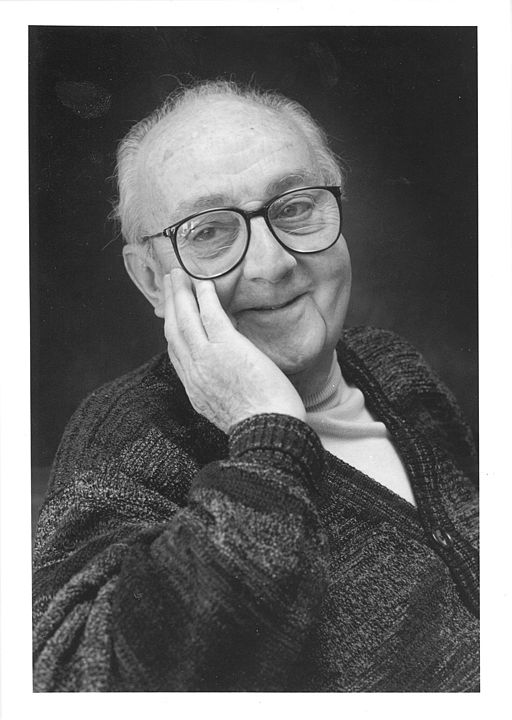
\includegraphics[width=0.9\columnwidth]{george_box.jpg}
        \end{column}
    \end{columns}
\end{frame}

\subsection{Fluxo de Trabalho Bayesiano (\textit{Workflow})\footnote{baseado em \textcite{gelmanBayesianWorkflow2020}}}
\begin{frame}{Fluxo de Trabalho Bayesiano (\textit{Workflow})\footnote{baseado em \textcite{gelmanBayesianWorkflow2020}}}
    \centering
    \begin{tikzpicture}[
        scale=0.8,
        transform shape, thick,
        every node/.style={text width=3.5cm, align=center},
        constructs/.style = {draw,
                            ellipse,
                            minimum width=4cm,
                            minimum height=2cm}
        ]
        \node[constructs] (Modelo) {Especificação do Modelo};
        \node[constructs] [right = of Modelo] (Priori) {Elicitação das \textit{Prioris}};
        \node[constructs] [right = of Priori] (Posterior) {Inferência da Posterior};
        \draw [<->, line width=1pt] (Modelo) to [out=45,in=135] node[above] {\textit{Prior Predictive Check}} (Priori);
        %\draw [->, line width=1pt] (Priori) to [out=225,in=315] {} (Modelo);
        \draw [<->, line width=1pt] (Priori) to [out=45,in=135] node[above] {\textit{Posterior Predictive Check}} (Posterior);
        %\draw [->, line width=1pt] (Posterior) to [out=225,in=315] {} (Priori);
    \end{tikzpicture}
\end{frame}

\subsection{Verificação Preditiva da \textit{Priori} (\textit{Prior Predictive Check})}
\begin{frame}{Verificação Preditiva da \textit{Priori} (\textit{Prior Predictive Check})}
    Em especial, antes de começar a alimentar o modelo com dados precisamos fazer uma
    checagem de todas as nossas \textit{prioris}.
    \vfill
    De maneira muito simples, consiste em simular parâmetros com base nas suas distribuições
    especificadas \textit{a priori} no modelo sem qualquer condicionamento aos dados e
    sem envolvimento nenhum da função de verossimilhança.
    \vfill
    Independentemente do nível de informação especificada na \textit{priori},
    é sempre importante realizar uma análise de sensibilidade prévia para entender completamente
    a influência que as \textit{prioris} têm na posterior.
\end{frame}

\begin{frame}{Verificação Preditiva da \textit{Priori} no \href{http://mc-stan.org/rstanarm/}{\texttt{rstanarm}} e \href{https://paul-buerkner.github.io/brms/}{\texttt{brms}}}
    \begin{vfilleditems}
        \item \texttt{rstanarm}: em qualquer função \text6t{stan\_*()} usar o argumento \texttt{prior\_PD = TRUE}
        \item \texttt{brms}: na função \textit{brm()} usar o argumento \texttt{sample\_prior = "only"}
    \end{vfilleditems}
\end{frame}

\subsubsection{Verificação Preditiva da \textit{Priori} no \texttt{rstanarm}}
\begin{frame}[fragile]{Verificação Preditiva da \textit{Priori} no \href{http://mc-stan.org/rstanarm/}{\texttt{rstanarm}}}
    \begin{lstlisting}
    stan_glm(y ~ ...,
        prior = normal(c(0, 0), c(5, 6)),
        prior_intercept = student_t(4, 0, 10),
        prior_aux = cauchy(0, 3),
        @prior_PD = TRUE@)
    \end{lstlisting}
\end{frame}
\subsubsection{Verificação Preditiva da \textit{Priori} no \texttt{brms}}
\begin{frame}[fragile]{Verificação Preditiva da \textit{Priori} no \href{https://paul-buerkner.github.io/brms/}{\texttt{brms}}}
    \begin{lstlisting}
    brm(y ~ x1 + x2,
        prior = c(
          prior(normal(0, 5), class = b, coef = x1),
          prior(normal(0, 6), class = b, coef = x2),
          prior(student_t(4, 0, 10), class = Intercept),
          prior(cauchy(0, 3), class = sigma)
        ),
        @sample_prior = "only"@)
    \end{lstlisting}
\end{frame}

\begin{frame}{Verificação Preditiva da \textit{Priori} no \href{https://paul-buerkner.github.io/brms/}{\texttt{brms}}}
    O interessante do \href{https://paul-buerkner.github.io/brms/}{\texttt{brms}} é
    que conseguimos naturalmente visualizar hipóteses sobre os valores do parâmetros de modelos
    estimados pela função \lstinline!brm()!
% library(brms)
% library(ggplot2)
% library(ggdark)
% library(bayesplot)
% library(tikzDevice)
% theme_set(dark_theme_light())
% bayesplot_theme_set(dark_theme_light())
% brms_custom_prior <- brm(mpg ~ wt + am, data = mtcars, chains = 1,
%  prior = c(
%    prior(normal(0, 5), class = b, coef = wt),
%    prior(normal(0, 6), class = b, coef = am),
%    prior(student_t(4, 0, 10), class = Intercept),
%    prior(cauchy(0, 3), class = sigma)
%  ),
%  sample_prior = "only")
% tikz(file = "slides/images/brms_prior_check.tex")
% plot(hypothesis(brms_custom_prior, "Intercept = 0"))
% dev.off()
    \begin{figure}
    \centering
        \resizebox{.35\linewidth}{!}{% Created by tikzDevice version 0.12.3.1 on 2021-05-29 18:08:38
% !TEX encoding = UTF-8 Unicode
\begin{tikzpicture}[x=1pt,y=1pt]
\definecolor{fillColor}{RGB}{255,255,255}
\path[use as bounding box,fill=fillColor,fill opacity=0.00] (0,0) rectangle (505.89,505.89);
\begin{scope}
\path[clip] (  0.00,  0.00) rectangle (505.89,505.89);
\definecolor{drawColor}{RGB}{0,0,0}
\definecolor{fillColor}{RGB}{0,0,0}

\path[draw=drawColor,line width= 0.6pt,line join=round,line cap=round,fill=fillColor] (  0.00,  0.00) rectangle (505.89,505.89);
\end{scope}
\begin{scope}
\path[clip] ( 20.71, 30.69) rectangle (423.76,483.82);
\definecolor{fillColor}{RGB}{0,0,0}

\path[fill=fillColor] ( 20.71, 30.69) rectangle (423.76,483.82);
\definecolor{drawColor}{gray}{0.13}

\path[draw=drawColor,line width= 0.1pt,line join=round] ( 20.71,102.37) --
	(423.76,102.37);

\path[draw=drawColor,line width= 0.1pt,line join=round] ( 20.71,204.55) --
	(423.76,204.55);

\path[draw=drawColor,line width= 0.1pt,line join=round] ( 20.71,306.73) --
	(423.76,306.73);

\path[draw=drawColor,line width= 0.1pt,line join=round] ( 20.71,408.90) --
	(423.76,408.90);

\path[draw=drawColor,line width= 0.1pt,line join=round] ( 61.13, 30.69) --
	( 61.13,483.82);

\path[draw=drawColor,line width= 0.1pt,line join=round] (146.15, 30.69) --
	(146.15,483.82);

\path[draw=drawColor,line width= 0.1pt,line join=round] (231.17, 30.69) --
	(231.17,483.82);

\path[draw=drawColor,line width= 0.1pt,line join=round] (316.19, 30.69) --
	(316.19,483.82);

\path[draw=drawColor,line width= 0.1pt,line join=round] (401.21, 30.69) --
	(401.21,483.82);

\path[draw=drawColor,line width= 0.3pt,line join=round] ( 20.71, 51.28) --
	(423.76, 51.28);

\path[draw=drawColor,line width= 0.3pt,line join=round] ( 20.71,153.46) --
	(423.76,153.46);

\path[draw=drawColor,line width= 0.3pt,line join=round] ( 20.71,255.64) --
	(423.76,255.64);

\path[draw=drawColor,line width= 0.3pt,line join=round] ( 20.71,357.81) --
	(423.76,357.81);

\path[draw=drawColor,line width= 0.3pt,line join=round] ( 20.71,459.99) --
	(423.76,459.99);

\path[draw=drawColor,line width= 0.3pt,line join=round] (103.64, 30.69) --
	(103.64,483.82);

\path[draw=drawColor,line width= 0.3pt,line join=round] (188.66, 30.69) --
	(188.66,483.82);

\path[draw=drawColor,line width= 0.3pt,line join=round] (273.68, 30.69) --
	(273.68,483.82);

\path[draw=drawColor,line width= 0.3pt,line join=round] (358.70, 30.69) --
	(358.70,483.82);
\definecolor{fillColor}{RGB}{0,91,150}

\path[fill=fillColor,fill opacity=0.70] ( 39.03, 53.02) --
	( 39.75, 53.01) --
	( 40.47, 52.99) --
	( 41.19, 52.96) --
	( 41.90, 52.92) --
	( 42.62, 52.87) --
	( 43.34, 52.81) --
	( 44.05, 52.75) --
	( 44.77, 52.68) --
	( 45.49, 52.61) --
	( 46.20, 52.54) --
	( 46.92, 52.47) --
	( 47.64, 52.41) --
	( 48.36, 52.36) --
	( 49.07, 52.32) --
	( 49.79, 52.29) --
	( 50.51, 52.28) --
	( 51.22, 52.29) --
	( 51.94, 52.31) --
	( 52.66, 52.36) --
	( 53.38, 52.42) --
	( 54.09, 52.51) --
	( 54.81, 52.63) --
	( 55.53, 52.77) --
	( 56.24, 52.93) --
	( 56.96, 53.11) --
	( 57.68, 53.31) --
	( 58.39, 53.53) --
	( 59.11, 53.77) --
	( 59.83, 54.02) --
	( 60.55, 54.28) --
	( 61.26, 54.54) --
	( 61.98, 54.81) --
	( 62.70, 55.07) --
	( 63.41, 55.32) --
	( 64.13, 55.55) --
	( 64.85, 55.76) --
	( 65.56, 55.95) --
	( 66.28, 56.11) --
	( 67.00, 56.24) --
	( 67.72, 56.33) --
	( 68.43, 56.39) --
	( 69.15, 56.40) --
	( 69.87, 56.38) --
	( 70.58, 56.31) --
	( 71.30, 56.21) --
	( 72.02, 56.08) --
	( 72.73, 55.91) --
	( 73.45, 55.71) --
	( 74.17, 55.49) --
	( 74.89, 55.25) --
	( 75.60, 54.99) --
	( 76.32, 54.73) --
	( 77.04, 54.46) --
	( 77.75, 54.18) --
	( 78.47, 53.91) --
	( 79.19, 53.65) --
	( 79.91, 53.40) --
	( 80.62, 53.16) --
	( 81.34, 52.93) --
	( 82.06, 52.72) --
	( 82.77, 52.53) --
	( 83.49, 52.35) --
	( 84.21, 52.19) --
	( 84.92, 52.05) --
	( 85.64, 51.93) --
	( 86.36, 51.82) --
	( 87.08, 51.73) --
	( 87.79, 51.65) --
	( 88.51, 51.58) --
	( 89.23, 51.53) --
	( 89.94, 51.48) --
	( 90.66, 51.44) --
	( 91.38, 51.41) --
	( 92.09, 51.38) --
	( 92.81, 51.37) --
	( 93.53, 51.35) --
	( 94.25, 51.34) --
	( 94.96, 51.34) --
	( 95.68, 51.34) --
	( 96.40, 51.34) --
	( 97.11, 51.35) --
	( 97.83, 51.36) --
	( 98.55, 51.37) --
	( 99.27, 51.39) --
	( 99.98, 51.41) --
	(100.70, 51.44) --
	(101.42, 51.47) --
	(102.13, 51.50) --
	(102.85, 51.55) --
	(103.57, 51.60) --
	(104.28, 51.65) --
	(105.00, 51.71) --
	(105.72, 51.78) --
	(106.44, 51.85) --
	(107.15, 51.93) --
	(107.87, 52.01) --
	(108.59, 52.10) --
	(109.30, 52.19) --
	(110.02, 52.28) --
	(110.74, 52.37) --
	(111.45, 52.47) --
	(112.17, 52.56) --
	(112.89, 52.64) --
	(113.61, 52.72) --
	(114.32, 52.80) --
	(115.04, 52.86) --
	(115.76, 52.92) --
	(116.47, 52.96) --
	(117.19, 52.99) --
	(117.91, 53.01) --
	(118.62, 53.01) --
	(119.34, 53.00) --
	(120.06, 52.98) --
	(120.78, 52.94) --
	(121.49, 52.89) --
	(122.21, 52.84) --
	(122.93, 52.77) --
	(123.64, 52.70) --
	(124.36, 52.62) --
	(125.08, 52.54) --
	(125.80, 52.45) --
	(126.51, 52.37) --
	(127.23, 52.29) --
	(127.95, 52.22) --
	(128.66, 52.16) --
	(129.38, 52.11) --
	(130.10, 52.06) --
	(130.81, 52.04) --
	(131.53, 52.03) --
	(132.25, 52.05) --
	(132.97, 52.08) --
	(133.68, 52.14) --
	(134.40, 52.23) --
	(135.12, 52.34) --
	(135.83, 52.49) --
	(136.55, 52.68) --
	(137.27, 52.90) --
	(137.98, 53.15) --
	(138.70, 53.45) --
	(139.42, 53.79) --
	(140.14, 54.16) --
	(140.85, 54.58) --
	(141.57, 55.04) --
	(142.29, 55.53) --
	(143.00, 56.05) --
	(143.72, 56.60) --
	(144.44, 57.18) --
	(145.16, 57.77) --
	(145.87, 58.37) --
	(146.59, 58.98) --
	(147.31, 59.57) --
	(148.02, 60.15) --
	(148.74, 60.70) --
	(149.46, 61.22) --
	(150.17, 61.70) --
	(150.89, 62.12) --
	(151.61, 62.49) --
	(152.33, 62.79) --
	(153.04, 63.04) --
	(153.76, 63.22) --
	(154.48, 63.33) --
	(155.19, 63.37) --
	(155.91, 63.34) --
	(156.63, 63.26) --
	(157.34, 63.13) --
	(158.06, 62.95) --
	(158.78, 62.74) --
	(159.50, 62.50) --
	(160.21, 62.24) --
	(160.93, 61.98) --
	(161.65, 61.72) --
	(162.36, 61.47) --
	(163.08, 61.23) --
	(163.80, 61.02) --
	(164.51, 60.84) --
	(165.23, 60.70) --
	(165.95, 60.59) --
	(166.67, 60.53) --
	(167.38, 60.50) --
	(168.10, 60.51) --
	(168.82, 60.56) --
	(169.53, 60.65) --
	(170.25, 60.77) --
	(170.97, 60.92) --
	(171.69, 61.11) --
	(172.40, 61.32) --
	(173.12, 61.56) --
	(173.84, 61.83) --
	(174.55, 62.13) --
	(175.27, 62.46) --
	(175.99, 62.83) --
	(176.70, 63.23) --
	(177.42, 63.68) --
	(178.14, 64.18) --
	(178.86, 64.73) --
	(179.57, 65.36) --
	(180.29, 66.05) --
	(181.01, 66.81) --
	(181.72, 67.65) --
	(182.44, 68.57) --
	(183.16, 69.58) --
	(183.87, 70.67) --
	(184.59, 71.85) --
	(185.31, 73.11) --
	(186.03, 74.45) --
	(186.74, 75.85) --
	(187.46, 77.32) --
	(188.18, 78.84) --
	(188.89, 80.41) --
	(189.61, 82.02) --
	(190.33, 83.65) --
	(191.05, 85.29) --
	(191.76, 86.94) --
	(192.48, 88.58) --
	(193.20, 90.22) --
	(193.91, 91.83) --
	(194.63, 93.43) --
	(195.35, 94.99) --
	(196.06, 96.53) --
	(196.78, 98.05) --
	(197.50, 99.54) --
	(198.22,101.02) --
	(198.93,102.47) --
	(199.65,103.91) --
	(200.37,105.35) --
	(201.08,106.79) --
	(201.80,108.23) --
	(202.52,109.69) --
	(203.23,111.16) --
	(203.95,112.65) --
	(204.67,114.17) --
	(205.39,115.71) --
	(206.10,117.28) --
	(206.82,118.87) --
	(207.54,120.50) --
	(208.25,122.15) --
	(208.97,123.83) --
	(209.69,125.53) --
	(210.40,127.27) --
	(211.12,129.04) --
	(211.84,130.84) --
	(212.56,132.68) --
	(213.27,134.58) --
	(213.99,136.54) --
	(214.71,138.56) --
	(215.42,140.67) --
	(216.14,142.86) --
	(216.86,145.15) --
	(217.58,147.56) --
	(218.29,150.11) --
	(219.01,152.81) --
	(219.73,155.66) --
	(220.44,158.67) --
	(221.16,161.85) --
	(221.88,165.19) --
	(222.59,168.73) --
	(223.31,172.45) --
	(224.03,176.33) --
	(224.75,180.37) --
	(225.46,184.56) --
	(226.18,188.89) --
	(226.90,193.35) --
	(227.61,197.93) --
	(228.33,202.61) --
	(229.05,207.37) --
	(229.76,212.19) --
	(230.48,217.06) --
	(231.20,221.96) --
	(231.92,226.90) --
	(232.63,231.84) --
	(233.35,236.80) --
	(234.07,241.74) --
	(234.78,246.68) --
	(235.50,251.60) --
	(236.22,256.50) --
	(236.94,261.38) --
	(237.65,266.24) --
	(238.37,271.07) --
	(239.09,275.87) --
	(239.80,280.66) --
	(240.52,285.42) --
	(241.24,290.16) --
	(241.95,294.89) --
	(242.67,299.61) --
	(243.39,304.32) --
	(244.11,309.04) --
	(244.82,313.77) --
	(245.54,318.53) --
	(246.26,323.31) --
	(246.97,328.15) --
	(247.69,333.04) --
	(248.41,338.00) --
	(249.12,343.03) --
	(249.84,348.14) --
	(250.56,353.32) --
	(251.28,358.59) --
	(251.99,363.95) --
	(252.71,369.38) --
	(253.43,374.86) --
	(254.14,380.38) --
	(254.86,385.92) --
	(255.58,391.46) --
	(256.29,396.97) --
	(257.01,402.41) --
	(257.73,407.77) --
	(258.45,413.01) --
	(259.16,418.10) --
	(259.88,423.02) --
	(260.60,427.74) --
	(261.31,432.21) --
	(262.03,436.43) --
	(262.75,440.37) --
	(263.47,444.05) --
	(264.18,447.43) --
	(264.90,450.52) --
	(265.62,453.30) --
	(266.33,455.70) --
	(267.05,457.78) --
	(267.77,459.53) --
	(268.48,460.96) --
	(269.20,462.06) --
	(269.92,462.82) --
	(270.64,463.21) --
	(271.35,463.22) --
	(272.07,462.89) --
	(272.79,462.21) --
	(273.50,461.19) --
	(274.22,459.84) --
	(274.94,458.16) --
	(275.65,456.11) --
	(276.37,453.73) --
	(277.09,451.07) --
	(277.81,448.14) --
	(278.52,444.96) --
	(279.24,441.57) --
	(279.96,437.97) --
	(280.67,434.19) --
	(281.39,430.29) --
	(282.11,426.29) --
	(282.83,422.23) --
	(283.54,418.14) --
	(284.26,414.05) --
	(284.98,409.97) --
	(285.69,405.95) --
	(286.41,401.99) --
	(287.13,398.10) --
	(287.84,394.30) --
	(288.56,390.57) --
	(289.28,386.94) --
	(290.00,383.38) --
	(290.71,379.90) --
	(291.43,376.47) --
	(292.15,373.07) --
	(292.86,369.69) --
	(293.58,366.31) --
	(294.30,362.91) --
	(295.01,359.45) --
	(295.73,355.93) --
	(296.45,352.32) --
	(297.17,348.61) --
	(297.88,344.79) --
	(298.60,340.84) --
	(299.32,336.76) --
	(300.03,332.52) --
	(300.75,328.13) --
	(301.47,323.61) --
	(302.18,318.95) --
	(302.90,314.16) --
	(303.62,309.26) --
	(304.34,304.24) --
	(305.05,299.12) --
	(305.77,293.93) --
	(306.49,288.69) --
	(307.20,283.41) --
	(307.92,278.11) --
	(308.64,272.82) --
	(309.36,267.57) --
	(310.07,262.36) --
	(310.79,257.23) --
	(311.51,252.19) --
	(312.22,247.26) --
	(312.94,242.44) --
	(313.66,237.76) --
	(314.37,233.24) --
	(315.09,228.88) --
	(315.81,224.67) --
	(316.53,220.60) --
	(317.24,216.69) --
	(317.96,212.92) --
	(318.68,209.29) --
	(319.39,205.81) --
	(320.11,202.43) --
	(320.83,199.16) --
	(321.54,195.98) --
	(322.26,192.88) --
	(322.98,189.85) --
	(323.70,186.88) --
	(324.41,183.96) --
	(325.13,181.09) --
	(325.85,178.25) --
	(326.56,175.44) --
	(327.28,172.67) --
	(328.00,169.92) --
	(328.72,167.21) --
	(329.43,164.52) --
	(330.15,161.86) --
	(330.87,159.23) --
	(331.58,156.63) --
	(332.30,154.06) --
	(333.02,151.51) --
	(333.73,148.98) --
	(334.45,146.48) --
	(335.17,144.00) --
	(335.89,141.54) --
	(336.60,139.09) --
	(337.32,136.65) --
	(338.04,134.23) --
	(338.75,131.81) --
	(339.47,129.41) --
	(340.19,127.02) --
	(340.90,124.65) --
	(341.62,122.29) --
	(342.34,119.96) --
	(343.06,117.66) --
	(343.77,115.40) --
	(344.49,113.17) --
	(345.21,111.00) --
	(345.92,108.88) --
	(346.64,106.82) --
	(347.36,104.82) --
	(348.07,102.91) --
	(348.79,101.08) --
	(349.51, 99.33) --
	(350.23, 97.65) --
	(350.94, 96.06) --
	(351.66, 94.55) --
	(352.38, 93.12) --
	(353.09, 91.78) --
	(353.81, 90.51) --
	(354.53, 89.31) --
	(355.25, 88.17) --
	(355.96, 87.09) --
	(356.68, 86.06) --
	(357.40, 85.07) --
	(358.11, 84.13) --
	(358.83, 83.21) --
	(359.55, 82.32) --
	(360.26, 81.45) --
	(360.98, 80.59) --
	(361.70, 79.75) --
	(362.42, 78.92) --
	(363.13, 78.10) --
	(363.85, 77.28) --
	(364.57, 76.48) --
	(365.28, 75.68) --
	(366.00, 74.90) --
	(366.72, 74.13) --
	(367.43, 73.38) --
	(368.15, 72.65) --
	(368.87, 71.94) --
	(369.59, 71.25) --
	(370.30, 70.59) --
	(371.02, 69.96) --
	(371.74, 69.35) --
	(372.45, 68.77) --
	(373.17, 68.22) --
	(373.89, 67.70) --
	(374.61, 67.20) --
	(375.32, 66.73) --
	(376.04, 66.27) --
	(376.76, 65.83) --
	(377.47, 65.40) --
	(378.19, 64.98) --
	(378.91, 64.57) --
	(379.62, 64.17) --
	(380.34, 63.76) --
	(381.06, 63.35) --
	(381.78, 62.94) --
	(382.49, 62.53) --
	(383.21, 62.11) --
	(383.93, 61.68) --
	(384.64, 61.25) --
	(385.36, 60.81) --
	(386.08, 60.37) --
	(386.79, 59.93) --
	(387.51, 59.49) --
	(388.23, 59.06) --
	(388.95, 58.63) --
	(389.66, 58.20) --
	(390.38, 57.79) --
	(391.10, 57.39) --
	(391.81, 57.01) --
	(392.53, 56.65) --
	(393.25, 56.31) --
	(393.96, 55.99) --
	(394.68, 55.69) --
	(395.40, 55.42) --
	(396.12, 55.17) --
	(396.83, 54.95) --
	(397.55, 54.74) --
	(398.27, 54.56) --
	(398.98, 54.40) --
	(399.70, 54.25) --
	(400.42, 54.12) --
	(401.14, 54.01) --
	(401.85, 53.90) --
	(402.57, 53.81) --
	(403.29, 53.72) --
	(404.00, 53.63) --
	(404.72, 53.55) --
	(405.44, 53.46) --
	(405.44, 51.28) --
	(404.72, 51.28) --
	(404.00, 51.28) --
	(403.29, 51.28) --
	(402.57, 51.28) --
	(401.85, 51.28) --
	(401.14, 51.28) --
	(400.42, 51.28) --
	(399.70, 51.28) --
	(398.98, 51.28) --
	(398.27, 51.28) --
	(397.55, 51.28) --
	(396.83, 51.28) --
	(396.12, 51.28) --
	(395.40, 51.28) --
	(394.68, 51.28) --
	(393.96, 51.28) --
	(393.25, 51.28) --
	(392.53, 51.28) --
	(391.81, 51.28) --
	(391.10, 51.28) --
	(390.38, 51.28) --
	(389.66, 51.28) --
	(388.95, 51.28) --
	(388.23, 51.28) --
	(387.51, 51.28) --
	(386.79, 51.28) --
	(386.08, 51.28) --
	(385.36, 51.28) --
	(384.64, 51.28) --
	(383.93, 51.28) --
	(383.21, 51.28) --
	(382.49, 51.28) --
	(381.78, 51.28) --
	(381.06, 51.28) --
	(380.34, 51.28) --
	(379.62, 51.28) --
	(378.91, 51.28) --
	(378.19, 51.28) --
	(377.47, 51.28) --
	(376.76, 51.28) --
	(376.04, 51.28) --
	(375.32, 51.28) --
	(374.61, 51.28) --
	(373.89, 51.28) --
	(373.17, 51.28) --
	(372.45, 51.28) --
	(371.74, 51.28) --
	(371.02, 51.28) --
	(370.30, 51.28) --
	(369.59, 51.28) --
	(368.87, 51.28) --
	(368.15, 51.28) --
	(367.43, 51.28) --
	(366.72, 51.28) --
	(366.00, 51.28) --
	(365.28, 51.28) --
	(364.57, 51.28) --
	(363.85, 51.28) --
	(363.13, 51.28) --
	(362.42, 51.28) --
	(361.70, 51.28) --
	(360.98, 51.28) --
	(360.26, 51.28) --
	(359.55, 51.28) --
	(358.83, 51.28) --
	(358.11, 51.28) --
	(357.40, 51.28) --
	(356.68, 51.28) --
	(355.96, 51.28) --
	(355.25, 51.28) --
	(354.53, 51.28) --
	(353.81, 51.28) --
	(353.09, 51.28) --
	(352.38, 51.28) --
	(351.66, 51.28) --
	(350.94, 51.28) --
	(350.23, 51.28) --
	(349.51, 51.28) --
	(348.79, 51.28) --
	(348.07, 51.28) --
	(347.36, 51.28) --
	(346.64, 51.28) --
	(345.92, 51.28) --
	(345.21, 51.28) --
	(344.49, 51.28) --
	(343.77, 51.28) --
	(343.06, 51.28) --
	(342.34, 51.28) --
	(341.62, 51.28) --
	(340.90, 51.28) --
	(340.19, 51.28) --
	(339.47, 51.28) --
	(338.75, 51.28) --
	(338.04, 51.28) --
	(337.32, 51.28) --
	(336.60, 51.28) --
	(335.89, 51.28) --
	(335.17, 51.28) --
	(334.45, 51.28) --
	(333.73, 51.28) --
	(333.02, 51.28) --
	(332.30, 51.28) --
	(331.58, 51.28) --
	(330.87, 51.28) --
	(330.15, 51.28) --
	(329.43, 51.28) --
	(328.72, 51.28) --
	(328.00, 51.28) --
	(327.28, 51.28) --
	(326.56, 51.28) --
	(325.85, 51.28) --
	(325.13, 51.28) --
	(324.41, 51.28) --
	(323.70, 51.28) --
	(322.98, 51.28) --
	(322.26, 51.28) --
	(321.54, 51.28) --
	(320.83, 51.28) --
	(320.11, 51.28) --
	(319.39, 51.28) --
	(318.68, 51.28) --
	(317.96, 51.28) --
	(317.24, 51.28) --
	(316.53, 51.28) --
	(315.81, 51.28) --
	(315.09, 51.28) --
	(314.37, 51.28) --
	(313.66, 51.28) --
	(312.94, 51.28) --
	(312.22, 51.28) --
	(311.51, 51.28) --
	(310.79, 51.28) --
	(310.07, 51.28) --
	(309.36, 51.28) --
	(308.64, 51.28) --
	(307.92, 51.28) --
	(307.20, 51.28) --
	(306.49, 51.28) --
	(305.77, 51.28) --
	(305.05, 51.28) --
	(304.34, 51.28) --
	(303.62, 51.28) --
	(302.90, 51.28) --
	(302.18, 51.28) --
	(301.47, 51.28) --
	(300.75, 51.28) --
	(300.03, 51.28) --
	(299.32, 51.28) --
	(298.60, 51.28) --
	(297.88, 51.28) --
	(297.17, 51.28) --
	(296.45, 51.28) --
	(295.73, 51.28) --
	(295.01, 51.28) --
	(294.30, 51.28) --
	(293.58, 51.28) --
	(292.86, 51.28) --
	(292.15, 51.28) --
	(291.43, 51.28) --
	(290.71, 51.28) --
	(290.00, 51.28) --
	(289.28, 51.28) --
	(288.56, 51.28) --
	(287.84, 51.28) --
	(287.13, 51.28) --
	(286.41, 51.28) --
	(285.69, 51.28) --
	(284.98, 51.28) --
	(284.26, 51.28) --
	(283.54, 51.28) --
	(282.83, 51.28) --
	(282.11, 51.28) --
	(281.39, 51.28) --
	(280.67, 51.28) --
	(279.96, 51.28) --
	(279.24, 51.28) --
	(278.52, 51.28) --
	(277.81, 51.28) --
	(277.09, 51.28) --
	(276.37, 51.28) --
	(275.65, 51.28) --
	(274.94, 51.28) --
	(274.22, 51.28) --
	(273.50, 51.28) --
	(272.79, 51.28) --
	(272.07, 51.28) --
	(271.35, 51.28) --
	(270.64, 51.28) --
	(269.92, 51.28) --
	(269.20, 51.28) --
	(268.48, 51.28) --
	(267.77, 51.28) --
	(267.05, 51.28) --
	(266.33, 51.28) --
	(265.62, 51.28) --
	(264.90, 51.28) --
	(264.18, 51.28) --
	(263.47, 51.28) --
	(262.75, 51.28) --
	(262.03, 51.28) --
	(261.31, 51.28) --
	(260.60, 51.28) --
	(259.88, 51.28) --
	(259.16, 51.28) --
	(258.45, 51.28) --
	(257.73, 51.28) --
	(257.01, 51.28) --
	(256.29, 51.28) --
	(255.58, 51.28) --
	(254.86, 51.28) --
	(254.14, 51.28) --
	(253.43, 51.28) --
	(252.71, 51.28) --
	(251.99, 51.28) --
	(251.28, 51.28) --
	(250.56, 51.28) --
	(249.84, 51.28) --
	(249.12, 51.28) --
	(248.41, 51.28) --
	(247.69, 51.28) --
	(246.97, 51.28) --
	(246.26, 51.28) --
	(245.54, 51.28) --
	(244.82, 51.28) --
	(244.11, 51.28) --
	(243.39, 51.28) --
	(242.67, 51.28) --
	(241.95, 51.28) --
	(241.24, 51.28) --
	(240.52, 51.28) --
	(239.80, 51.28) --
	(239.09, 51.28) --
	(238.37, 51.28) --
	(237.65, 51.28) --
	(236.94, 51.28) --
	(236.22, 51.28) --
	(235.50, 51.28) --
	(234.78, 51.28) --
	(234.07, 51.28) --
	(233.35, 51.28) --
	(232.63, 51.28) --
	(231.92, 51.28) --
	(231.20, 51.28) --
	(230.48, 51.28) --
	(229.76, 51.28) --
	(229.05, 51.28) --
	(228.33, 51.28) --
	(227.61, 51.28) --
	(226.90, 51.28) --
	(226.18, 51.28) --
	(225.46, 51.28) --
	(224.75, 51.28) --
	(224.03, 51.28) --
	(223.31, 51.28) --
	(222.59, 51.28) --
	(221.88, 51.28) --
	(221.16, 51.28) --
	(220.44, 51.28) --
	(219.73, 51.28) --
	(219.01, 51.28) --
	(218.29, 51.28) --
	(217.58, 51.28) --
	(216.86, 51.28) --
	(216.14, 51.28) --
	(215.42, 51.28) --
	(214.71, 51.28) --
	(213.99, 51.28) --
	(213.27, 51.28) --
	(212.56, 51.28) --
	(211.84, 51.28) --
	(211.12, 51.28) --
	(210.40, 51.28) --
	(209.69, 51.28) --
	(208.97, 51.28) --
	(208.25, 51.28) --
	(207.54, 51.28) --
	(206.82, 51.28) --
	(206.10, 51.28) --
	(205.39, 51.28) --
	(204.67, 51.28) --
	(203.95, 51.28) --
	(203.23, 51.28) --
	(202.52, 51.28) --
	(201.80, 51.28) --
	(201.08, 51.28) --
	(200.37, 51.28) --
	(199.65, 51.28) --
	(198.93, 51.28) --
	(198.22, 51.28) --
	(197.50, 51.28) --
	(196.78, 51.28) --
	(196.06, 51.28) --
	(195.35, 51.28) --
	(194.63, 51.28) --
	(193.91, 51.28) --
	(193.20, 51.28) --
	(192.48, 51.28) --
	(191.76, 51.28) --
	(191.05, 51.28) --
	(190.33, 51.28) --
	(189.61, 51.28) --
	(188.89, 51.28) --
	(188.18, 51.28) --
	(187.46, 51.28) --
	(186.74, 51.28) --
	(186.03, 51.28) --
	(185.31, 51.28) --
	(184.59, 51.28) --
	(183.87, 51.28) --
	(183.16, 51.28) --
	(182.44, 51.28) --
	(181.72, 51.28) --
	(181.01, 51.28) --
	(180.29, 51.28) --
	(179.57, 51.28) --
	(178.86, 51.28) --
	(178.14, 51.28) --
	(177.42, 51.28) --
	(176.70, 51.28) --
	(175.99, 51.28) --
	(175.27, 51.28) --
	(174.55, 51.28) --
	(173.84, 51.28) --
	(173.12, 51.28) --
	(172.40, 51.28) --
	(171.69, 51.28) --
	(170.97, 51.28) --
	(170.25, 51.28) --
	(169.53, 51.28) --
	(168.82, 51.28) --
	(168.10, 51.28) --
	(167.38, 51.28) --
	(166.67, 51.28) --
	(165.95, 51.28) --
	(165.23, 51.28) --
	(164.51, 51.28) --
	(163.80, 51.28) --
	(163.08, 51.28) --
	(162.36, 51.28) --
	(161.65, 51.28) --
	(160.93, 51.28) --
	(160.21, 51.28) --
	(159.50, 51.28) --
	(158.78, 51.28) --
	(158.06, 51.28) --
	(157.34, 51.28) --
	(156.63, 51.28) --
	(155.91, 51.28) --
	(155.19, 51.28) --
	(154.48, 51.28) --
	(153.76, 51.28) --
	(153.04, 51.28) --
	(152.33, 51.28) --
	(151.61, 51.28) --
	(150.89, 51.28) --
	(150.17, 51.28) --
	(149.46, 51.28) --
	(148.74, 51.28) --
	(148.02, 51.28) --
	(147.31, 51.28) --
	(146.59, 51.28) --
	(145.87, 51.28) --
	(145.16, 51.28) --
	(144.44, 51.28) --
	(143.72, 51.28) --
	(143.00, 51.28) --
	(142.29, 51.28) --
	(141.57, 51.28) --
	(140.85, 51.28) --
	(140.14, 51.28) --
	(139.42, 51.28) --
	(138.70, 51.28) --
	(137.98, 51.28) --
	(137.27, 51.28) --
	(136.55, 51.28) --
	(135.83, 51.28) --
	(135.12, 51.28) --
	(134.40, 51.28) --
	(133.68, 51.28) --
	(132.97, 51.28) --
	(132.25, 51.28) --
	(131.53, 51.28) --
	(130.81, 51.28) --
	(130.10, 51.28) --
	(129.38, 51.28) --
	(128.66, 51.28) --
	(127.95, 51.28) --
	(127.23, 51.28) --
	(126.51, 51.28) --
	(125.80, 51.28) --
	(125.08, 51.28) --
	(124.36, 51.28) --
	(123.64, 51.28) --
	(122.93, 51.28) --
	(122.21, 51.28) --
	(121.49, 51.28) --
	(120.78, 51.28) --
	(120.06, 51.28) --
	(119.34, 51.28) --
	(118.62, 51.28) --
	(117.91, 51.28) --
	(117.19, 51.28) --
	(116.47, 51.28) --
	(115.76, 51.28) --
	(115.04, 51.28) --
	(114.32, 51.28) --
	(113.61, 51.28) --
	(112.89, 51.28) --
	(112.17, 51.28) --
	(111.45, 51.28) --
	(110.74, 51.28) --
	(110.02, 51.28) --
	(109.30, 51.28) --
	(108.59, 51.28) --
	(107.87, 51.28) --
	(107.15, 51.28) --
	(106.44, 51.28) --
	(105.72, 51.28) --
	(105.00, 51.28) --
	(104.28, 51.28) --
	(103.57, 51.28) --
	(102.85, 51.28) --
	(102.13, 51.28) --
	(101.42, 51.28) --
	(100.70, 51.28) --
	( 99.98, 51.28) --
	( 99.27, 51.28) --
	( 98.55, 51.28) --
	( 97.83, 51.28) --
	( 97.11, 51.28) --
	( 96.40, 51.28) --
	( 95.68, 51.28) --
	( 94.96, 51.28) --
	( 94.25, 51.28) --
	( 93.53, 51.28) --
	( 92.81, 51.28) --
	( 92.09, 51.28) --
	( 91.38, 51.28) --
	( 90.66, 51.28) --
	( 89.94, 51.28) --
	( 89.23, 51.28) --
	( 88.51, 51.28) --
	( 87.79, 51.28) --
	( 87.08, 51.28) --
	( 86.36, 51.28) --
	( 85.64, 51.28) --
	( 84.92, 51.28) --
	( 84.21, 51.28) --
	( 83.49, 51.28) --
	( 82.77, 51.28) --
	( 82.06, 51.28) --
	( 81.34, 51.28) --
	( 80.62, 51.28) --
	( 79.91, 51.28) --
	( 79.19, 51.28) --
	( 78.47, 51.28) --
	( 77.75, 51.28) --
	( 77.04, 51.28) --
	( 76.32, 51.28) --
	( 75.60, 51.28) --
	( 74.89, 51.28) --
	( 74.17, 51.28) --
	( 73.45, 51.28) --
	( 72.73, 51.28) --
	( 72.02, 51.28) --
	( 71.30, 51.28) --
	( 70.58, 51.28) --
	( 69.87, 51.28) --
	( 69.15, 51.28) --
	( 68.43, 51.28) --
	( 67.72, 51.28) --
	( 67.00, 51.28) --
	( 66.28, 51.28) --
	( 65.56, 51.28) --
	( 64.85, 51.28) --
	( 64.13, 51.28) --
	( 63.41, 51.28) --
	( 62.70, 51.28) --
	( 61.98, 51.28) --
	( 61.26, 51.28) --
	( 60.55, 51.28) --
	( 59.83, 51.28) --
	( 59.11, 51.28) --
	( 58.39, 51.28) --
	( 57.68, 51.28) --
	( 56.96, 51.28) --
	( 56.24, 51.28) --
	( 55.53, 51.28) --
	( 54.81, 51.28) --
	( 54.09, 51.28) --
	( 53.38, 51.28) --
	( 52.66, 51.28) --
	( 51.94, 51.28) --
	( 51.22, 51.28) --
	( 50.51, 51.28) --
	( 49.79, 51.28) --
	( 49.07, 51.28) --
	( 48.36, 51.28) --
	( 47.64, 51.28) --
	( 46.92, 51.28) --
	( 46.20, 51.28) --
	( 45.49, 51.28) --
	( 44.77, 51.28) --
	( 44.05, 51.28) --
	( 43.34, 51.28) --
	( 42.62, 51.28) --
	( 41.90, 51.28) --
	( 41.19, 51.28) --
	( 40.47, 51.28) --
	( 39.75, 51.28) --
	( 39.03, 51.28) --
	cycle;
\definecolor{drawColor}{RGB}{255,255,255}

\path[draw=drawColor,line width= 0.6pt,line join=round,line cap=round] ( 39.03, 53.02) --
	( 39.75, 53.01) --
	( 40.47, 52.99) --
	( 41.19, 52.96) --
	( 41.90, 52.92) --
	( 42.62, 52.87) --
	( 43.34, 52.81) --
	( 44.05, 52.75) --
	( 44.77, 52.68) --
	( 45.49, 52.61) --
	( 46.20, 52.54) --
	( 46.92, 52.47) --
	( 47.64, 52.41) --
	( 48.36, 52.36) --
	( 49.07, 52.32) --
	( 49.79, 52.29) --
	( 50.51, 52.28) --
	( 51.22, 52.29) --
	( 51.94, 52.31) --
	( 52.66, 52.36) --
	( 53.38, 52.42) --
	( 54.09, 52.51) --
	( 54.81, 52.63) --
	( 55.53, 52.77) --
	( 56.24, 52.93) --
	( 56.96, 53.11) --
	( 57.68, 53.31) --
	( 58.39, 53.53) --
	( 59.11, 53.77) --
	( 59.83, 54.02) --
	( 60.55, 54.28) --
	( 61.26, 54.54) --
	( 61.98, 54.81) --
	( 62.70, 55.07) --
	( 63.41, 55.32) --
	( 64.13, 55.55) --
	( 64.85, 55.76) --
	( 65.56, 55.95) --
	( 66.28, 56.11) --
	( 67.00, 56.24) --
	( 67.72, 56.33) --
	( 68.43, 56.39) --
	( 69.15, 56.40) --
	( 69.87, 56.38) --
	( 70.58, 56.31) --
	( 71.30, 56.21) --
	( 72.02, 56.08) --
	( 72.73, 55.91) --
	( 73.45, 55.71) --
	( 74.17, 55.49) --
	( 74.89, 55.25) --
	( 75.60, 54.99) --
	( 76.32, 54.73) --
	( 77.04, 54.46) --
	( 77.75, 54.18) --
	( 78.47, 53.91) --
	( 79.19, 53.65) --
	( 79.91, 53.40) --
	( 80.62, 53.16) --
	( 81.34, 52.93) --
	( 82.06, 52.72) --
	( 82.77, 52.53) --
	( 83.49, 52.35) --
	( 84.21, 52.19) --
	( 84.92, 52.05) --
	( 85.64, 51.93) --
	( 86.36, 51.82) --
	( 87.08, 51.73) --
	( 87.79, 51.65) --
	( 88.51, 51.58) --
	( 89.23, 51.53) --
	( 89.94, 51.48) --
	( 90.66, 51.44) --
	( 91.38, 51.41) --
	( 92.09, 51.38) --
	( 92.81, 51.37) --
	( 93.53, 51.35) --
	( 94.25, 51.34) --
	( 94.96, 51.34) --
	( 95.68, 51.34) --
	( 96.40, 51.34) --
	( 97.11, 51.35) --
	( 97.83, 51.36) --
	( 98.55, 51.37) --
	( 99.27, 51.39) --
	( 99.98, 51.41) --
	(100.70, 51.44) --
	(101.42, 51.47) --
	(102.13, 51.50) --
	(102.85, 51.55) --
	(103.57, 51.60) --
	(104.28, 51.65) --
	(105.00, 51.71) --
	(105.72, 51.78) --
	(106.44, 51.85) --
	(107.15, 51.93) --
	(107.87, 52.01) --
	(108.59, 52.10) --
	(109.30, 52.19) --
	(110.02, 52.28) --
	(110.74, 52.37) --
	(111.45, 52.47) --
	(112.17, 52.56) --
	(112.89, 52.64) --
	(113.61, 52.72) --
	(114.32, 52.80) --
	(115.04, 52.86) --
	(115.76, 52.92) --
	(116.47, 52.96) --
	(117.19, 52.99) --
	(117.91, 53.01) --
	(118.62, 53.01) --
	(119.34, 53.00) --
	(120.06, 52.98) --
	(120.78, 52.94) --
	(121.49, 52.89) --
	(122.21, 52.84) --
	(122.93, 52.77) --
	(123.64, 52.70) --
	(124.36, 52.62) --
	(125.08, 52.54) --
	(125.80, 52.45) --
	(126.51, 52.37) --
	(127.23, 52.29) --
	(127.95, 52.22) --
	(128.66, 52.16) --
	(129.38, 52.11) --
	(130.10, 52.06) --
	(130.81, 52.04) --
	(131.53, 52.03) --
	(132.25, 52.05) --
	(132.97, 52.08) --
	(133.68, 52.14) --
	(134.40, 52.23) --
	(135.12, 52.34) --
	(135.83, 52.49) --
	(136.55, 52.68) --
	(137.27, 52.90) --
	(137.98, 53.15) --
	(138.70, 53.45) --
	(139.42, 53.79) --
	(140.14, 54.16) --
	(140.85, 54.58) --
	(141.57, 55.04) --
	(142.29, 55.53) --
	(143.00, 56.05) --
	(143.72, 56.60) --
	(144.44, 57.18) --
	(145.16, 57.77) --
	(145.87, 58.37) --
	(146.59, 58.98) --
	(147.31, 59.57) --
	(148.02, 60.15) --
	(148.74, 60.70) --
	(149.46, 61.22) --
	(150.17, 61.70) --
	(150.89, 62.12) --
	(151.61, 62.49) --
	(152.33, 62.79) --
	(153.04, 63.04) --
	(153.76, 63.22) --
	(154.48, 63.33) --
	(155.19, 63.37) --
	(155.91, 63.34) --
	(156.63, 63.26) --
	(157.34, 63.13) --
	(158.06, 62.95) --
	(158.78, 62.74) --
	(159.50, 62.50) --
	(160.21, 62.24) --
	(160.93, 61.98) --
	(161.65, 61.72) --
	(162.36, 61.47) --
	(163.08, 61.23) --
	(163.80, 61.02) --
	(164.51, 60.84) --
	(165.23, 60.70) --
	(165.95, 60.59) --
	(166.67, 60.53) --
	(167.38, 60.50) --
	(168.10, 60.51) --
	(168.82, 60.56) --
	(169.53, 60.65) --
	(170.25, 60.77) --
	(170.97, 60.92) --
	(171.69, 61.11) --
	(172.40, 61.32) --
	(173.12, 61.56) --
	(173.84, 61.83) --
	(174.55, 62.13) --
	(175.27, 62.46) --
	(175.99, 62.83) --
	(176.70, 63.23) --
	(177.42, 63.68) --
	(178.14, 64.18) --
	(178.86, 64.73) --
	(179.57, 65.36) --
	(180.29, 66.05) --
	(181.01, 66.81) --
	(181.72, 67.65) --
	(182.44, 68.57) --
	(183.16, 69.58) --
	(183.87, 70.67) --
	(184.59, 71.85) --
	(185.31, 73.11) --
	(186.03, 74.45) --
	(186.74, 75.85) --
	(187.46, 77.32) --
	(188.18, 78.84) --
	(188.89, 80.41) --
	(189.61, 82.02) --
	(190.33, 83.65) --
	(191.05, 85.29) --
	(191.76, 86.94) --
	(192.48, 88.58) --
	(193.20, 90.22) --
	(193.91, 91.83) --
	(194.63, 93.43) --
	(195.35, 94.99) --
	(196.06, 96.53) --
	(196.78, 98.05) --
	(197.50, 99.54) --
	(198.22,101.02) --
	(198.93,102.47) --
	(199.65,103.91) --
	(200.37,105.35) --
	(201.08,106.79) --
	(201.80,108.23) --
	(202.52,109.69) --
	(203.23,111.16) --
	(203.95,112.65) --
	(204.67,114.17) --
	(205.39,115.71) --
	(206.10,117.28) --
	(206.82,118.87) --
	(207.54,120.50) --
	(208.25,122.15) --
	(208.97,123.83) --
	(209.69,125.53) --
	(210.40,127.27) --
	(211.12,129.04) --
	(211.84,130.84) --
	(212.56,132.68) --
	(213.27,134.58) --
	(213.99,136.54) --
	(214.71,138.56) --
	(215.42,140.67) --
	(216.14,142.86) --
	(216.86,145.15) --
	(217.58,147.56) --
	(218.29,150.11) --
	(219.01,152.81) --
	(219.73,155.66) --
	(220.44,158.67) --
	(221.16,161.85) --
	(221.88,165.19) --
	(222.59,168.73) --
	(223.31,172.45) --
	(224.03,176.33) --
	(224.75,180.37) --
	(225.46,184.56) --
	(226.18,188.89) --
	(226.90,193.35) --
	(227.61,197.93) --
	(228.33,202.61) --
	(229.05,207.37) --
	(229.76,212.19) --
	(230.48,217.06) --
	(231.20,221.96) --
	(231.92,226.90) --
	(232.63,231.84) --
	(233.35,236.80) --
	(234.07,241.74) --
	(234.78,246.68) --
	(235.50,251.60) --
	(236.22,256.50) --
	(236.94,261.38) --
	(237.65,266.24) --
	(238.37,271.07) --
	(239.09,275.87) --
	(239.80,280.66) --
	(240.52,285.42) --
	(241.24,290.16) --
	(241.95,294.89) --
	(242.67,299.61) --
	(243.39,304.32) --
	(244.11,309.04) --
	(244.82,313.77) --
	(245.54,318.53) --
	(246.26,323.31) --
	(246.97,328.15) --
	(247.69,333.04) --
	(248.41,338.00) --
	(249.12,343.03) --
	(249.84,348.14) --
	(250.56,353.32) --
	(251.28,358.59) --
	(251.99,363.95) --
	(252.71,369.38) --
	(253.43,374.86) --
	(254.14,380.38) --
	(254.86,385.92) --
	(255.58,391.46) --
	(256.29,396.97) --
	(257.01,402.41) --
	(257.73,407.77) --
	(258.45,413.01) --
	(259.16,418.10) --
	(259.88,423.02) --
	(260.60,427.74) --
	(261.31,432.21) --
	(262.03,436.43) --
	(262.75,440.37) --
	(263.47,444.05) --
	(264.18,447.43) --
	(264.90,450.52) --
	(265.62,453.30) --
	(266.33,455.70) --
	(267.05,457.78) --
	(267.77,459.53) --
	(268.48,460.96) --
	(269.20,462.06) --
	(269.92,462.82) --
	(270.64,463.21) --
	(271.35,463.22) --
	(272.07,462.89) --
	(272.79,462.21) --
	(273.50,461.19) --
	(274.22,459.84) --
	(274.94,458.16) --
	(275.65,456.11) --
	(276.37,453.73) --
	(277.09,451.07) --
	(277.81,448.14) --
	(278.52,444.96) --
	(279.24,441.57) --
	(279.96,437.97) --
	(280.67,434.19) --
	(281.39,430.29) --
	(282.11,426.29) --
	(282.83,422.23) --
	(283.54,418.14) --
	(284.26,414.05) --
	(284.98,409.97) --
	(285.69,405.95) --
	(286.41,401.99) --
	(287.13,398.10) --
	(287.84,394.30) --
	(288.56,390.57) --
	(289.28,386.94) --
	(290.00,383.38) --
	(290.71,379.90) --
	(291.43,376.47) --
	(292.15,373.07) --
	(292.86,369.69) --
	(293.58,366.31) --
	(294.30,362.91) --
	(295.01,359.45) --
	(295.73,355.93) --
	(296.45,352.32) --
	(297.17,348.61) --
	(297.88,344.79) --
	(298.60,340.84) --
	(299.32,336.76) --
	(300.03,332.52) --
	(300.75,328.13) --
	(301.47,323.61) --
	(302.18,318.95) --
	(302.90,314.16) --
	(303.62,309.26) --
	(304.34,304.24) --
	(305.05,299.12) --
	(305.77,293.93) --
	(306.49,288.69) --
	(307.20,283.41) --
	(307.92,278.11) --
	(308.64,272.82) --
	(309.36,267.57) --
	(310.07,262.36) --
	(310.79,257.23) --
	(311.51,252.19) --
	(312.22,247.26) --
	(312.94,242.44) --
	(313.66,237.76) --
	(314.37,233.24) --
	(315.09,228.88) --
	(315.81,224.67) --
	(316.53,220.60) --
	(317.24,216.69) --
	(317.96,212.92) --
	(318.68,209.29) --
	(319.39,205.81) --
	(320.11,202.43) --
	(320.83,199.16) --
	(321.54,195.98) --
	(322.26,192.88) --
	(322.98,189.85) --
	(323.70,186.88) --
	(324.41,183.96) --
	(325.13,181.09) --
	(325.85,178.25) --
	(326.56,175.44) --
	(327.28,172.67) --
	(328.00,169.92) --
	(328.72,167.21) --
	(329.43,164.52) --
	(330.15,161.86) --
	(330.87,159.23) --
	(331.58,156.63) --
	(332.30,154.06) --
	(333.02,151.51) --
	(333.73,148.98) --
	(334.45,146.48) --
	(335.17,144.00) --
	(335.89,141.54) --
	(336.60,139.09) --
	(337.32,136.65) --
	(338.04,134.23) --
	(338.75,131.81) --
	(339.47,129.41) --
	(340.19,127.02) --
	(340.90,124.65) --
	(341.62,122.29) --
	(342.34,119.96) --
	(343.06,117.66) --
	(343.77,115.40) --
	(344.49,113.17) --
	(345.21,111.00) --
	(345.92,108.88) --
	(346.64,106.82) --
	(347.36,104.82) --
	(348.07,102.91) --
	(348.79,101.08) --
	(349.51, 99.33) --
	(350.23, 97.65) --
	(350.94, 96.06) --
	(351.66, 94.55) --
	(352.38, 93.12) --
	(353.09, 91.78) --
	(353.81, 90.51) --
	(354.53, 89.31) --
	(355.25, 88.17) --
	(355.96, 87.09) --
	(356.68, 86.06) --
	(357.40, 85.07) --
	(358.11, 84.13) --
	(358.83, 83.21) --
	(359.55, 82.32) --
	(360.26, 81.45) --
	(360.98, 80.59) --
	(361.70, 79.75) --
	(362.42, 78.92) --
	(363.13, 78.10) --
	(363.85, 77.28) --
	(364.57, 76.48) --
	(365.28, 75.68) --
	(366.00, 74.90) --
	(366.72, 74.13) --
	(367.43, 73.38) --
	(368.15, 72.65) --
	(368.87, 71.94) --
	(369.59, 71.25) --
	(370.30, 70.59) --
	(371.02, 69.96) --
	(371.74, 69.35) --
	(372.45, 68.77) --
	(373.17, 68.22) --
	(373.89, 67.70) --
	(374.61, 67.20) --
	(375.32, 66.73) --
	(376.04, 66.27) --
	(376.76, 65.83) --
	(377.47, 65.40) --
	(378.19, 64.98) --
	(378.91, 64.57) --
	(379.62, 64.17) --
	(380.34, 63.76) --
	(381.06, 63.35) --
	(381.78, 62.94) --
	(382.49, 62.53) --
	(383.21, 62.11) --
	(383.93, 61.68) --
	(384.64, 61.25) --
	(385.36, 60.81) --
	(386.08, 60.37) --
	(386.79, 59.93) --
	(387.51, 59.49) --
	(388.23, 59.06) --
	(388.95, 58.63) --
	(389.66, 58.20) --
	(390.38, 57.79) --
	(391.10, 57.39) --
	(391.81, 57.01) --
	(392.53, 56.65) --
	(393.25, 56.31) --
	(393.96, 55.99) --
	(394.68, 55.69) --
	(395.40, 55.42) --
	(396.12, 55.17) --
	(396.83, 54.95) --
	(397.55, 54.74) --
	(398.27, 54.56) --
	(398.98, 54.40) --
	(399.70, 54.25) --
	(400.42, 54.12) --
	(401.14, 54.01) --
	(401.85, 53.90) --
	(402.57, 53.81) --
	(403.29, 53.72) --
	(404.00, 53.63) --
	(404.72, 53.55) --
	(405.44, 53.46);
\definecolor{drawColor}{RGB}{76,76,76}

\path[draw=drawColor,line width= 0.6pt,line join=round,line cap=round] ( 20.71, 30.69) rectangle (423.76,483.82);
\end{scope}
\begin{scope}
\path[clip] ( 20.71,483.82) rectangle (423.76,500.39);
\definecolor{fillColor}{RGB}{76,76,76}

\path[fill=fillColor] ( 20.71,483.82) rectangle (423.76,500.39);
\definecolor{drawColor}{RGB}{0,0,0}

\node[text=drawColor,anchor=base,inner sep=0pt, outer sep=0pt, scale=  0.88] at (222.24,489.07) {(Intercept) = 0};
\end{scope}
\begin{scope}
\path[clip] (  0.00,  0.00) rectangle (505.89,505.89);
\definecolor{drawColor}{RGB}{76,76,76}

\path[draw=drawColor,line width= 0.3pt,line join=round] (103.64, 27.94) --
	(103.64, 30.69);

\path[draw=drawColor,line width= 0.3pt,line join=round] (188.66, 27.94) --
	(188.66, 30.69);

\path[draw=drawColor,line width= 0.3pt,line join=round] (273.68, 27.94) --
	(273.68, 30.69);

\path[draw=drawColor,line width= 0.3pt,line join=round] (358.70, 27.94) --
	(358.70, 30.69);
\end{scope}
\begin{scope}
\path[clip] (  0.00,  0.00) rectangle (505.89,505.89);
\definecolor{drawColor}{RGB}{178,178,178}

\node[text=drawColor,anchor=base,inner sep=0pt, outer sep=0pt, scale=  0.88] at (103.64, 19.68) {-100};

\node[text=drawColor,anchor=base,inner sep=0pt, outer sep=0pt, scale=  0.88] at (188.66, 19.68) {-50};

\node[text=drawColor,anchor=base,inner sep=0pt, outer sep=0pt, scale=  0.88] at (273.68, 19.68) {0};

\node[text=drawColor,anchor=base,inner sep=0pt, outer sep=0pt, scale=  0.88] at (358.70, 19.68) {50};
\end{scope}
\begin{scope}
\path[clip] (  0.00,  0.00) rectangle (505.89,505.89);
\definecolor{fillColor}{RGB}{0,0,0}

\path[fill=fillColor] (434.76,236.92) rectangle (500.39,277.59);
\end{scope}
\begin{scope}
\path[clip] (  0.00,  0.00) rectangle (505.89,505.89);
\definecolor{drawColor}{RGB}{255,255,255}

\node[text=drawColor,anchor=base west,inner sep=0pt, outer sep=0pt, scale=  1.10] at (440.26,263.44) {Type};
\end{scope}
\begin{scope}
\path[clip] (  0.00,  0.00) rectangle (505.89,505.89);
\definecolor{fillColor}{RGB}{0,0,0}

\path[fill=fillColor] (440.26,242.42) rectangle (454.71,256.87);
\end{scope}
\begin{scope}
\path[clip] (  0.00,  0.00) rectangle (505.89,505.89);
\definecolor{drawColor}{RGB}{255,255,255}
\definecolor{fillColor}{RGB}{0,91,150}

\path[draw=drawColor,line width= 0.6pt,line cap=rect,fill=fillColor,fill opacity=0.70] (440.97,243.13) rectangle (454.00,256.16);
\end{scope}
\begin{scope}
\path[clip] (  0.00,  0.00) rectangle (505.89,505.89);
\definecolor{drawColor}{RGB}{255,255,255}

\node[text=drawColor,anchor=base west,inner sep=0pt, outer sep=0pt, scale=  0.88] at (460.21,246.61) {Posterior};
\end{scope}
\end{tikzpicture}
}
    \end{figure}
\end{frame}

\subsection{Verificação Preditiva da Posterior (\textit{Posterior Predictive Check})}
\begin{frame}{Verificação Preditiva da Posterior (\textit{Posterior Predictive Check})}
    Precisamos nos certificar que a nossa distribuição posterior de $\boldsymbol{y}$
    consegue capturar todas as nuanças da densidade real de $\boldsymbol{y}$.
    \vfill
    Isto é um procedimento chamado de Verificação Preditiva da Posterior
    (\textit{Posterior Predictive Check}) e é geralmente auferido com uma inspeção
    visual\footnote{também fazemos inspeções matemáticas probabilísticas,
    veja a seção de Comparação de Modelos} da densidade real de $\boldsymbol{y}$
    contrastada com amostragens da densidade
    posterior de $\boldsymbol{y}$ estimada pelo modelo Bayesiano.
    \vfill
    O propósito é comparar o histograma da variável dependente $\boldsymbol{y}$ contra o histograma variáveis dependentes simuladas
    pelo modelo $\boldsymbol{y}_{\text{rep}}$ após a estimação dos parâmetros. A ideia é
    que os histogramas reais e simulados se misturem e não haja divergências.
\end{frame}

\begin{frame}{Verificação Preditiva da Posterior no \href{http://mc-stan.org/rstanarm/}{\texttt{rstanarm}} e \href{https://paul-buerkner.github.io/brms/}{\texttt{brms}}}
    \begin{vfilleditems}
        \item \texttt{rstanarm}: função \lstinline!pp_check()! em qualquer modelo oriundo das funções \lstinline!stan_*()!
        \item \texttt{brms}: função \lstinline!pp_check()! em qualquer modelo oriundo da função \lstinline!brm()!
    \end{vfilleditems}
\end{frame}

\subsubsection{Verificação Preditiva da Posterior no \texttt{rstanarm}}
\begin{frame}[fragile]{Verificação Preditiva da Posterior no \href{http://mc-stan.org/rstanarm/}{\texttt{rstanarm}}}
    \begin{lstlisting}
    rstanarm_fit <- stan_glm(mpg ~ wt + am, data = mtcars)
    @pp_check(rstanarm_fit)@
    \end{lstlisting}
\end{frame}

\begin{frame}{Verificação Preditiva da Posterior no \href{http://mc-stan.org/rstanarm/}{\texttt{rstanarm}}}
% library(rstanarm)
% library(ggplot2)
% library(ggdark)
% library(bayesplot)
% library(tikzDevice)
% theme_set(dark_theme_light())
% bayesplot_theme_set(dark_theme_light())
% rstanarm_fit <- stan_glm(mpg ~ wt + am, data = mtcars)
% tikz(file = "slides/images/pp_check_rstanarm.tex")
% pp_check(rstanarm_fit, nreps = 10, seed = 123, type = "dens_overlay")
% dev.off()
    \begin{columns}
        \begin{column}{0.5\textwidth}
            \begin{figure}
                \centering
                \resizebox{0.8\columnwidth}{!}{% Created by tikzDevice version 0.12.3.1 on 2021-06-01 06:51:52
% !TEX encoding = UTF-8 Unicode
\begin{tikzpicture}[x=1pt,y=1pt]
\definecolor{fillColor}{RGB}{255,255,255}
\path[use as bounding box,fill=fillColor,fill opacity=0.00] (0,0) rectangle (505.89,505.89);
\begin{scope}
\path[clip] (  0.00,  0.00) rectangle (505.89,505.89);
\definecolor{drawColor}{RGB}{0,0,0}
\definecolor{fillColor}{RGB}{0,0,0}

\path[draw=drawColor,line width= 0.6pt,line join=round,line cap=round,fill=fillColor] (  0.00,  0.00) rectangle (505.89,505.89);
\end{scope}
\begin{scope}
\path[clip] (  8.25, 18.22) rectangle (445.03,500.39);
\definecolor{fillColor}{RGB}{0,0,0}

\path[fill=fillColor] (  8.25, 18.22) rectangle (445.03,500.39);
\definecolor{drawColor}{gray}{0.13}

\path[draw=drawColor,line width= 0.1pt,line join=round] (  8.25, 80.15) --
	(445.03, 80.15);

\path[draw=drawColor,line width= 0.1pt,line join=round] (  8.25,204.29) --
	(445.03,204.29);

\path[draw=drawColor,line width= 0.1pt,line join=round] (  8.25,328.43) --
	(445.03,328.43);

\path[draw=drawColor,line width= 0.1pt,line join=round] (  8.25,452.57) --
	(445.03,452.57);

\path[draw=drawColor,line width= 0.1pt,line join=round] ( 25.56, 18.22) --
	( 25.56,500.39);

\path[draw=drawColor,line width= 0.1pt,line join=round] (168.91, 18.22) --
	(168.91,500.39);

\path[draw=drawColor,line width= 0.1pt,line join=round] (312.26, 18.22) --
	(312.26,500.39);

\path[draw=drawColor,line width= 0.3pt,line join=round] (  8.25,142.22) --
	(445.03,142.22);

\path[draw=drawColor,line width= 0.3pt,line join=round] (  8.25,266.36) --
	(445.03,266.36);

\path[draw=drawColor,line width= 0.3pt,line join=round] (  8.25,390.50) --
	(445.03,390.50);

\path[draw=drawColor,line width= 0.3pt,line join=round] ( 97.24, 18.22) --
	( 97.24,500.39);

\path[draw=drawColor,line width= 0.3pt,line join=round] (240.58, 18.22) --
	(240.58,500.39);

\path[draw=drawColor,line width= 0.3pt,line join=round] (383.93, 18.22) --
	(383.93,500.39);
\definecolor{drawColor}{RGB}{179,205,224}

\path[draw=drawColor,draw opacity=0.70,line width= 0.3pt,line join=round] (  8.25, 81.87) --
	(  8.68, 82.38) --
	(  9.10, 82.90) --
	(  9.53, 83.42) --
	(  9.96, 83.93) --
	( 10.38, 84.44) --
	( 10.81, 84.96) --
	( 11.24, 85.47) --
	( 11.67, 85.97) --
	( 12.09, 86.48) --
	( 12.52, 86.98) --
	( 12.95, 87.49) --
	( 13.37, 87.99) --
	( 13.80, 88.48) --
	( 14.23, 88.98) --
	( 14.65, 89.47) --
	( 15.08, 89.97) --
	( 15.51, 90.45) --
	( 15.94, 90.94) --
	( 16.36, 91.42) --
	( 16.79, 91.91) --
	( 17.22, 92.38) --
	( 17.64, 92.86) --
	( 18.07, 93.33) --
	( 18.50, 93.80) --
	( 18.92, 94.27) --
	( 19.35, 94.73) --
	( 19.78, 95.19) --
	( 20.20, 95.65) --
	( 20.63, 96.10) --
	( 21.06, 96.55) --
	( 21.49, 97.00) --
	( 21.91, 97.44) --
	( 22.34, 97.88) --
	( 22.77, 98.32) --
	( 23.19, 98.75) --
	( 23.62, 99.18) --
	( 24.05, 99.60) --
	( 24.47,100.02) --
	( 24.90,100.44) --
	( 25.33,100.85) --
	( 25.76,101.26) --
	( 26.18,101.66) --
	( 26.61,102.06) --
	( 27.04,102.46) --
	( 27.46,102.85) --
	( 27.89,103.23) --
	( 28.32,103.61) --
	( 28.74,103.99) --
	( 29.17,104.36) --
	( 29.60,104.73) --
	( 30.02,105.09) --
	( 30.45,105.45) --
	( 30.88,105.80) --
	( 31.31,106.15) --
	( 31.73,106.49) --
	( 32.16,106.83) --
	( 32.59,107.16) --
	( 33.01,107.49) --
	( 33.44,107.81) --
	( 33.87,108.12) --
	( 34.29,108.44) --
	( 34.72,108.74) --
	( 35.15,109.04) --
	( 35.58,109.34) --
	( 36.00,109.62) --
	( 36.43,109.91) --
	( 36.86,110.19) --
	( 37.28,110.46) --
	( 37.71,110.73) --
	( 38.14,110.99) --
	( 38.56,111.24) --
	( 38.99,111.49) --
	( 39.42,111.74) --
	( 39.84,111.98) --
	( 40.27,112.21) --
	( 40.70,112.43) --
	( 41.13,112.66) --
	( 41.55,112.87) --
	( 41.98,113.08) --
	( 42.41,113.28) --
	( 42.83,113.48) --
	( 43.26,113.67) --
	( 43.69,113.86) --
	( 44.11,114.04) --
	( 44.54,114.21) --
	( 44.97,114.38) --
	( 45.40,114.54) --
	( 45.82,114.70) --
	( 46.25,114.85) --
	( 46.68,114.99) --
	( 47.10,115.13) --
	( 47.53,115.26) --
	( 47.96,115.39) --
	( 48.38,115.51) --
	( 48.81,115.62) --
	( 49.24,115.73) --
	( 49.66,115.84) --
	( 50.09,115.94) --
	( 50.52,116.03) --
	( 50.95,116.11) --
	( 51.37,116.20) --
	( 51.80,116.27) --
	( 52.23,116.34) --
	( 52.65,116.41) --
	( 53.08,116.46) --
	( 53.51,116.52) --
	( 53.93,116.56) --
	( 54.36,116.61) --
	( 54.79,116.65) --
	( 55.22,116.68) --
	( 55.64,116.70) --
	( 56.07,116.73) --
	( 56.50,116.74) --
	( 56.92,116.75) --
	( 57.35,116.76) --
	( 57.78,116.76) --
	( 58.20,116.76) --
	( 58.63,116.75) --
	( 59.06,116.74) --
	( 59.48,116.72) --
	( 59.91,116.70) --
	( 60.34,116.67) --
	( 60.77,116.64) --
	( 61.19,116.60) --
	( 61.62,116.56) --
	( 62.05,116.52) --
	( 62.47,116.47) --
	( 62.90,116.42) --
	( 63.33,116.36) --
	( 63.75,116.30) --
	( 64.18,116.24) --
	( 64.61,116.17) --
	( 65.04,116.10) --
	( 65.46,116.02) --
	( 65.89,115.94) --
	( 66.32,115.86) --
	( 66.74,115.77) --
	( 67.17,115.68) --
	( 67.60,115.59) --
	( 68.02,115.50) --
	( 68.45,115.40) --
	( 68.88,115.30) --
	( 69.30,115.19) --
	( 69.73,115.08) --
	( 70.16,114.97) --
	( 70.59,114.86) --
	( 71.01,114.74) --
	( 71.44,114.63) --
	( 71.87,114.51) --
	( 72.29,114.38) --
	( 72.72,114.26) --
	( 73.15,114.13) --
	( 73.57,114.00) --
	( 74.00,113.87) --
	( 74.43,113.74) --
	( 74.86,113.61) --
	( 75.28,113.47) --
	( 75.71,113.33) --
	( 76.14,113.19) --
	( 76.56,113.05) --
	( 76.99,112.91) --
	( 77.42,112.77) --
	( 77.84,112.62) --
	( 78.27,112.48) --
	( 78.70,112.33) --
	( 79.12,112.19) --
	( 79.55,112.04) --
	( 79.98,111.89) --
	( 80.41,111.74) --
	( 80.83,111.59) --
	( 81.26,111.44) --
	( 81.69,111.29) --
	( 82.11,111.14) --
	( 82.54,110.99) --
	( 82.97,110.84) --
	( 83.39,110.68) --
	( 83.82,110.53) --
	( 84.25,110.38) --
	( 84.68,110.23) --
	( 85.10,110.08) --
	( 85.53,109.93) --
	( 85.96,109.78) --
	( 86.38,109.63) --
	( 86.81,109.48) --
	( 87.24,109.33) --
	( 87.66,109.19) --
	( 88.09,109.04) --
	( 88.52,108.89) --
	( 88.94,108.75) --
	( 89.37,108.61) --
	( 89.80,108.46) --
	( 90.23,108.32) --
	( 90.65,108.18) --
	( 91.08,108.05) --
	( 91.51,107.91) --
	( 91.93,107.77) --
	( 92.36,107.64) --
	( 92.79,107.51) --
	( 93.21,107.38) --
	( 93.64,107.25) --
	( 94.07,107.13) --
	( 94.49,107.01) --
	( 94.92,106.88) --
	( 95.35,106.77) --
	( 95.78,106.65) --
	( 96.20,106.53) --
	( 96.63,106.42) --
	( 97.06,106.32) --
	( 97.48,106.21) --
	( 97.91,106.11) --
	( 98.34,106.01) --
	( 98.76,105.91) --
	( 99.19,105.82) --
	( 99.62,105.73) --
	(100.05,105.64) --
	(100.47,105.56) --
	(100.90,105.48) --
	(101.33,105.40) --
	(101.75,105.33) --
	(102.18,105.26) --
	(102.61,105.20) --
	(103.03,105.14) --
	(103.46,105.08) --
	(103.89,105.03) --
	(104.31,104.98) --
	(104.74,104.94) --
	(105.17,104.90) --
	(105.60,104.87) --
	(106.02,104.84) --
	(106.45,104.82) --
	(106.88,104.80) --
	(107.30,104.79) --
	(107.73,104.79) --
	(108.16,104.79) --
	(108.58,104.79) --
	(109.01,104.80) --
	(109.44,104.82) --
	(109.87,104.84) --
	(110.29,104.87) --
	(110.72,104.91) --
	(111.15,104.95) --
	(111.57,105.00) --
	(112.00,105.06) --
	(112.43,105.13) --
	(112.85,105.20) --
	(113.28,105.28) --
	(113.71,105.36) --
	(114.13,105.46) --
	(114.56,105.56) --
	(114.99,105.67) --
	(115.42,105.79) --
	(115.84,105.92) --
	(116.27,106.05) --
	(116.70,106.20) --
	(117.12,106.35) --
	(117.55,106.51) --
	(117.98,106.69) --
	(118.40,106.87) --
	(118.83,107.06) --
	(119.26,107.26) --
	(119.69,107.47) --
	(120.11,107.70) --
	(120.54,107.93) --
	(120.97,108.17) --
	(121.39,108.43) --
	(121.82,108.69) --
	(122.25,108.97) --
	(122.67,109.26) --
	(123.10,109.55) --
	(123.53,109.87) --
	(123.95,110.19) --
	(124.38,110.52) --
	(124.81,110.87) --
	(125.24,111.23) --
	(125.66,111.61) --
	(126.09,111.99) --
	(126.52,112.39) --
	(126.94,112.80) --
	(127.37,113.23) --
	(127.80,113.67) --
	(128.22,114.12) --
	(128.65,114.59) --
	(129.08,115.07) --
	(129.51,115.57) --
	(129.93,116.08) --
	(130.36,116.61) --
	(130.79,117.15) --
	(131.21,117.70) --
	(131.64,118.28) --
	(132.07,118.86) --
	(132.49,119.46) --
	(132.92,120.08) --
	(133.35,120.71) --
	(133.77,121.37) --
	(134.20,122.03) --
	(134.63,122.71) --
	(135.06,123.41) --
	(135.48,124.13) --
	(135.91,124.86) --
	(136.34,125.61) --
	(136.76,126.38) --
	(137.19,127.17) --
	(137.62,127.97) --
	(138.04,128.78) --
	(138.47,129.62) --
	(138.90,130.47) --
	(139.33,131.35) --
	(139.75,132.24) --
	(140.18,133.14) --
	(140.61,134.08) --
	(141.03,135.02) --
	(141.46,135.98) --
	(141.89,136.96) --
	(142.31,137.96) --
	(142.74,138.98) --
	(143.17,140.02) --
	(143.59,141.07) --
	(144.02,142.15) --
	(144.45,143.24) --
	(144.88,144.35) --
	(145.30,145.48) --
	(145.73,146.63) --
	(146.16,147.80) --
	(146.58,148.98) --
	(147.01,150.19) --
	(147.44,151.41) --
	(147.86,152.65) --
	(148.29,153.92) --
	(148.72,155.20) --
	(149.15,156.49) --
	(149.57,157.81) --
	(150.00,159.15) --
	(150.43,160.50) --
	(150.85,161.87) --
	(151.28,163.26) --
	(151.71,164.67) --
	(152.13,166.10) --
	(152.56,167.54) --
	(152.99,169.01) --
	(153.41,170.49) --
	(153.84,171.99) --
	(154.27,173.51) --
	(154.70,175.03) --
	(155.12,176.59) --
	(155.55,178.16) --
	(155.98,179.74) --
	(156.40,181.35) --
	(156.83,182.96) --
	(157.26,184.60) --
	(157.68,186.25) --
	(158.11,187.92) --
	(158.54,189.61) --
	(158.97,191.30) --
	(159.39,193.02) --
	(159.82,194.75) --
	(160.25,196.49) --
	(160.67,198.26) --
	(161.10,200.03) --
	(161.53,201.82) --
	(161.95,203.63) --
	(162.38,205.44) --
	(162.81,207.27) --
	(163.23,209.12) --
	(163.66,210.97) --
	(164.09,212.85) --
	(164.52,214.73) --
	(164.94,216.62) --
	(165.37,218.53) --
	(165.80,220.45) --
	(166.22,222.38) --
	(166.65,224.32) --
	(167.08,226.27) --
	(167.50,228.24) --
	(167.93,230.21) --
	(168.36,232.19) --
	(168.79,234.18) --
	(169.21,236.18) --
	(169.64,238.19) --
	(170.07,240.21) --
	(170.49,242.24) --
	(170.92,244.27) --
	(171.35,246.31) --
	(171.77,248.36) --
	(172.20,250.41) --
	(172.63,252.47) --
	(173.05,254.54) --
	(173.48,256.61) --
	(173.91,258.69) --
	(174.34,260.77) --
	(174.76,262.86) --
	(175.19,264.95) --
	(175.62,267.05) --
	(176.04,269.14) --
	(176.47,271.24) --
	(176.90,273.35) --
	(177.32,275.45) --
	(177.75,277.56) --
	(178.18,279.67) --
	(178.61,281.78) --
	(179.03,283.89) --
	(179.46,286.00) --
	(179.89,288.11) --
	(180.31,290.22) --
	(180.74,292.33) --
	(181.17,294.44) --
	(181.59,296.55) --
	(182.02,298.65) --
	(182.45,300.75) --
	(182.87,302.85) --
	(183.30,304.95) --
	(183.73,307.04) --
	(184.16,309.13) --
	(184.58,311.22) --
	(185.01,313.30) --
	(185.44,315.37) --
	(185.86,317.44) --
	(186.29,319.51) --
	(186.72,321.57) --
	(187.14,323.62) --
	(187.57,325.67) --
	(188.00,327.70) --
	(188.43,329.74) --
	(188.85,331.76) --
	(189.28,333.78) --
	(189.71,335.78) --
	(190.13,337.78) --
	(190.56,339.77) --
	(190.99,341.75) --
	(191.41,343.72) --
	(191.84,345.69) --
	(192.27,347.64) --
	(192.69,349.58) --
	(193.12,351.51) --
	(193.55,353.42) --
	(193.98,355.33) --
	(194.40,357.23) --
	(194.83,359.11) --
	(195.26,360.98) --
	(195.68,362.84) --
	(196.11,364.69) --
	(196.54,366.52) --
	(196.96,368.34) --
	(197.39,370.14) --
	(197.82,371.93) --
	(198.25,373.71) --
	(198.67,375.48) --
	(199.10,377.22) --
	(199.53,378.96) --
	(199.95,380.68) --
	(200.38,382.38) --
	(200.81,384.07) --
	(201.23,385.74) --
	(201.66,387.40) --
	(202.09,389.04) --
	(202.51,390.66) --
	(202.94,392.27) --
	(203.37,393.86) --
	(203.80,395.43) --
	(204.22,397.00) --
	(204.65,398.53) --
	(205.08,400.06) --
	(205.50,401.56) --
	(205.93,403.05) --
	(206.36,404.52) --
	(206.78,405.97) --
	(207.21,407.41) --
	(207.64,408.82) --
	(208.07,410.22) --
	(208.49,411.60) --
	(208.92,412.96) --
	(209.35,414.30) --
	(209.77,415.63) --
	(210.20,416.93) --
	(210.63,418.21) --
	(211.05,419.48) --
	(211.48,420.73) --
	(211.91,421.96) --
	(212.33,423.16) --
	(212.76,424.35) --
	(213.19,425.53) --
	(213.62,426.67) --
	(214.04,427.80) --
	(214.47,428.91) --
	(214.90,430.00) --
	(215.32,431.08) --
	(215.75,432.13) --
	(216.18,433.16) --
	(216.60,434.17) --
	(217.03,435.16) --
	(217.46,436.14) --
	(217.89,437.09) --
	(218.31,438.02) --
	(218.74,438.94) --
	(219.17,439.82) --
	(219.59,440.70) --
	(220.02,441.55) --
	(220.45,442.38) --
	(220.87,443.20) --
	(221.30,443.99) --
	(221.73,444.76) --
	(222.15,445.52) --
	(222.58,446.25) --
	(223.01,446.97) --
	(223.44,447.66) --
	(223.86,448.33) --
	(224.29,448.99) --
	(224.72,449.63) --
	(225.14,450.24) --
	(225.57,450.84) --
	(226.00,451.42) --
	(226.42,451.98) --
	(226.85,452.52) --
	(227.28,453.04) --
	(227.71,453.54) --
	(228.13,454.02) --
	(228.56,454.48) --
	(228.99,454.93) --
	(229.41,455.35) --
	(229.84,455.76) --
	(230.27,456.15) --
	(230.69,456.52) --
	(231.12,456.88) --
	(231.55,457.21) --
	(231.97,457.52) --
	(232.40,457.82) --
	(232.83,458.10) --
	(233.26,458.37) --
	(233.68,458.61) --
	(234.11,458.84) --
	(234.54,459.05) --
	(234.96,459.24) --
	(235.39,459.42) --
	(235.82,459.58) --
	(236.24,459.72) --
	(236.67,459.85) --
	(237.10,459.95) --
	(237.53,460.05) --
	(237.95,460.13) --
	(238.38,460.19) --
	(238.81,460.23) --
	(239.23,460.26) --
	(239.66,460.27) --
	(240.09,460.28) --
	(240.51,460.26) --
	(240.94,460.23) --
	(241.37,460.18) --
	(241.79,460.12) --
	(242.22,460.04) --
	(242.65,459.95) --
	(243.08,459.85) --
	(243.50,459.73) --
	(243.93,459.59) --
	(244.36,459.45) --
	(244.78,459.29) --
	(245.21,459.11) --
	(245.64,458.93) --
	(246.06,458.73) --
	(246.49,458.51) --
	(246.92,458.29) --
	(247.35,458.05) --
	(247.77,457.80) --
	(248.20,457.54) --
	(248.63,457.26) --
	(249.05,456.97) --
	(249.48,456.67) --
	(249.91,456.36) --
	(250.33,456.04) --
	(250.76,455.70) --
	(251.19,455.36) --
	(251.61,455.00) --
	(252.04,454.63) --
	(252.47,454.26) --
	(252.90,453.87) --
	(253.32,453.47) --
	(253.75,453.06) --
	(254.18,452.64) --
	(254.60,452.21) --
	(255.03,451.77) --
	(255.46,451.31) --
	(255.88,450.86) --
	(256.31,450.39) --
	(256.74,449.91) --
	(257.17,449.42) --
	(257.59,448.92) --
	(258.02,448.41) --
	(258.45,447.90) --
	(258.87,447.37) --
	(259.30,446.84) --
	(259.73,446.30) --
	(260.15,445.75) --
	(260.58,445.19) --
	(261.01,444.62) --
	(261.43,444.04) --
	(261.86,443.46) --
	(262.29,442.86) --
	(262.72,442.26) --
	(263.14,441.65) --
	(263.57,441.04) --
	(264.00,440.41) --
	(264.42,439.78) --
	(264.85,439.14) --
	(265.28,438.49) --
	(265.70,437.83) --
	(266.13,437.17) --
	(266.56,436.50) --
	(266.98,435.82) --
	(267.41,435.13) --
	(267.84,434.44) --
	(268.27,433.74) --
	(268.69,433.03) --
	(269.12,432.31) --
	(269.55,431.59) --
	(269.97,430.86) --
	(270.40,430.12) --
	(270.83,429.37) --
	(271.25,428.62) --
	(271.68,427.86) --
	(272.11,427.09) --
	(272.54,426.32) --
	(272.96,425.54) --
	(273.39,424.75) --
	(273.82,423.95) --
	(274.24,423.14) --
	(274.67,422.33) --
	(275.10,421.51) --
	(275.52,420.69) --
	(275.95,419.85) --
	(276.38,419.01) --
	(276.80,418.16) --
	(277.23,417.31) --
	(277.66,416.44) --
	(278.09,415.57) --
	(278.51,414.69) --
	(278.94,413.80) --
	(279.37,412.91) --
	(279.79,412.00) --
	(280.22,411.09) --
	(280.65,410.18) --
	(281.07,409.25) --
	(281.50,408.31) --
	(281.93,407.37) --
	(282.36,406.42) --
	(282.78,405.46) --
	(283.21,404.50) --
	(283.64,403.52) --
	(284.06,402.54) --
	(284.49,401.55) --
	(284.92,400.55) --
	(285.34,399.54) --
	(285.77,398.52) --
	(286.20,397.50) --
	(286.62,396.47) --
	(287.05,395.43) --
	(287.48,394.38) --
	(287.91,393.32) --
	(288.33,392.25) --
	(288.76,391.18) --
	(289.19,390.09) --
	(289.61,389.00) --
	(290.04,387.90) --
	(290.47,386.79) --
	(290.89,385.67) --
	(291.32,384.54) --
	(291.75,383.41) --
	(292.18,382.26) --
	(292.60,381.10) --
	(293.03,379.94) --
	(293.46,378.77) --
	(293.88,377.59) --
	(294.31,376.40) --
	(294.74,375.20) --
	(295.16,374.00) --
	(295.59,372.78) --
	(296.02,371.55) --
	(296.44,370.32) --
	(296.87,369.08) --
	(297.30,367.83) --
	(297.73,366.57) --
	(298.15,365.30) --
	(298.58,364.03) --
	(299.01,362.74) --
	(299.43,361.45) --
	(299.86,360.14) --
	(300.29,358.83) --
	(300.71,357.51) --
	(301.14,356.19) --
	(301.57,354.85) --
	(302.00,353.51) --
	(302.42,352.15) --
	(302.85,350.80) --
	(303.28,349.43) --
	(303.70,348.05) --
	(304.13,346.67) --
	(304.56,345.28) --
	(304.98,343.88) --
	(305.41,342.47) --
	(305.84,341.06) --
	(306.26,339.64) --
	(306.69,338.21) --
	(307.12,336.77) --
	(307.55,335.33) --
	(307.97,333.88) --
	(308.40,332.43) --
	(308.83,330.97) --
	(309.25,329.50) --
	(309.68,328.02) --
	(310.11,326.54) --
	(310.53,325.05) --
	(310.96,323.56) --
	(311.39,322.06) --
	(311.82,320.56) --
	(312.24,319.05) --
	(312.67,317.54) --
	(313.10,316.02) --
	(313.52,314.49) --
	(313.95,312.96) --
	(314.38,311.43) --
	(314.80,309.89) --
	(315.23,308.35) --
	(315.66,306.81) --
	(316.08,305.26) --
	(316.51,303.70) --
	(316.94,302.15) --
	(317.37,300.59) --
	(317.79,299.02) --
	(318.22,297.46) --
	(318.65,295.89) --
	(319.07,294.32) --
	(319.50,292.74) --
	(319.93,291.17) --
	(320.35,289.59) --
	(320.78,288.01) --
	(321.21,286.43) --
	(321.64,284.85) --
	(322.06,283.27) --
	(322.49,281.68) --
	(322.92,280.10) --
	(323.34,278.52) --
	(323.77,276.93) --
	(324.20,275.34) --
	(324.62,273.76) --
	(325.05,272.17) --
	(325.48,270.59) --
	(325.90,269.01) --
	(326.33,267.42) --
	(326.76,265.84) --
	(327.19,264.26) --
	(327.61,262.68) --
	(328.04,261.10) --
	(328.47,259.53) --
	(328.89,257.95) --
	(329.32,256.38) --
	(329.75,254.81) --
	(330.17,253.25) --
	(330.60,251.68) --
	(331.03,250.12) --
	(331.46,248.56) --
	(331.88,247.01) --
	(332.31,245.46) --
	(332.74,243.91) --
	(333.16,242.36) --
	(333.59,240.82) --
	(334.02,239.29) --
	(334.44,237.76) --
	(334.87,236.23) --
	(335.30,234.71) --
	(335.72,233.19) --
	(336.15,231.68) --
	(336.58,230.17) --
	(337.01,228.66) --
	(337.43,227.17) --
	(337.86,225.67) --
	(338.29,224.19) --
	(338.71,222.71) --
	(339.14,221.23) --
	(339.57,219.76) --
	(339.99,218.30) --
	(340.42,216.84) --
	(340.85,215.39) --
	(341.28,213.94) --
	(341.70,212.51) --
	(342.13,211.07) --
	(342.56,209.65) --
	(342.98,208.23) --
	(343.41,206.82) --
	(343.84,205.42) --
	(344.26,204.02) --
	(344.69,202.63) --
	(345.12,201.25) --
	(345.54,199.87) --
	(345.97,198.50) --
	(346.40,197.14) --
	(346.83,195.79) --
	(347.25,194.44) --
	(347.68,193.10) --
	(348.11,191.77) --
	(348.53,190.45) --
	(348.96,189.13) --
	(349.39,187.83) --
	(349.81,186.53) --
	(350.24,185.23) --
	(350.67,183.95) --
	(351.10,182.68) --
	(351.52,181.41) --
	(351.95,180.15) --
	(352.38,178.90) --
	(352.80,177.66) --
	(353.23,176.42) --
	(353.66,175.19) --
	(354.08,173.98) --
	(354.51,172.77) --
	(354.94,171.56) --
	(355.36,170.37) --
	(355.79,169.18) --
	(356.22,168.01) --
	(356.65,166.84) --
	(357.07,165.67) --
	(357.50,164.52) --
	(357.93,163.38) --
	(358.35,162.24) --
	(358.78,161.11) --
	(359.21,159.99) --
	(359.63,158.88) --
	(360.06,157.77) --
	(360.49,156.68) --
	(360.92,155.59) --
	(361.34,154.51) --
	(361.77,153.44) --
	(362.20,152.38) --
	(362.62,151.32) --
	(363.05,150.27) --
	(363.48,149.23) --
	(363.90,148.20) --
	(364.33,147.18) --
	(364.76,146.16) --
	(365.18,145.15) --
	(365.61,144.15) --
	(366.04,143.16) --
	(366.47,142.17) --
	(366.89,141.20) --
	(367.32,140.22) --
	(367.75,139.26) --
	(368.17,138.31) --
	(368.60,137.36) --
	(369.03,136.42) --
	(369.45,135.49) --
	(369.88,134.56) --
	(370.31,133.64) --
	(370.74,132.73) --
	(371.16,131.83) --
	(371.59,130.93) --
	(372.02,130.04) --
	(372.44,129.16) --
	(372.87,128.28) --
	(373.30,127.42) --
	(373.72,126.55) --
	(374.15,125.70) --
	(374.58,124.85) --
	(375.00,124.01) --
	(375.43,123.17) --
	(375.86,122.35) --
	(376.29,121.52) --
	(376.71,120.71) --
	(377.14,119.90) --
	(377.57,119.09) --
	(377.99,118.30) --
	(378.42,117.50) --
	(378.85,116.72) --
	(379.27,115.94) --
	(379.70,115.17) --
	(380.13,114.40) --
	(380.56,113.64) --
	(380.98,112.89) --
	(381.41,112.14) --
	(381.84,111.39) --
	(382.26,110.65) --
	(382.69,109.92) --
	(383.12,109.19) --
	(383.54,108.47) --
	(383.97,107.75) --
	(384.40,107.04) --
	(384.82,106.33) --
	(385.25,105.63) --
	(385.68,104.93) --
	(386.11,104.24) --
	(386.53,103.55) --
	(386.96,102.87) --
	(387.39,102.19) --
	(387.81,101.52) --
	(388.24,100.85) --
	(388.67,100.19) --
	(389.09, 99.53) --
	(389.52, 98.87) --
	(389.95, 98.23) --
	(390.38, 97.58) --
	(390.80, 96.94) --
	(391.23, 96.30) --
	(391.66, 95.66) --
	(392.08, 95.03) --
	(392.51, 94.41) --
	(392.94, 93.79) --
	(393.36, 93.17) --
	(393.79, 92.55) --
	(394.22, 91.94) --
	(394.64, 91.34) --
	(395.07, 90.73) --
	(395.50, 90.13) --
	(395.93, 89.54) --
	(396.35, 88.94) --
	(396.78, 88.35) --
	(397.21, 87.77) --
	(397.63, 87.18) --
	(398.06, 86.60) --
	(398.49, 86.02) --
	(398.91, 85.45) --
	(399.34, 84.88) --
	(399.77, 84.31) --
	(400.20, 83.75) --
	(400.62, 83.18) --
	(401.05, 82.62) --
	(401.48, 82.07) --
	(401.90, 81.51) --
	(402.33, 80.96) --
	(402.76, 80.41) --
	(403.18, 79.87) --
	(403.61, 79.32) --
	(404.04, 78.78) --
	(404.46, 78.24) --
	(404.89, 77.71) --
	(405.32, 77.17) --
	(405.75, 76.64) --
	(406.17, 76.11) --
	(406.60, 75.59) --
	(407.03, 75.06) --
	(407.45, 74.54) --
	(407.88, 74.02) --
	(408.31, 73.50) --
	(408.73, 72.98) --
	(409.16, 72.47) --
	(409.59, 71.96) --
	(410.02, 71.45) --
	(410.44, 70.94) --
	(410.87, 70.43) --
	(411.30, 69.93) --
	(411.72, 69.43) --
	(412.15, 68.93) --
	(412.58, 68.43) --
	(413.00, 67.94) --
	(413.43, 67.44) --
	(413.86, 66.95) --
	(414.28, 66.46) --
	(414.71, 65.97) --
	(415.14, 65.48) --
	(415.57, 65.00) --
	(415.99, 64.52) --
	(416.42, 64.03) --
	(416.85, 63.56) --
	(417.27, 63.08) --
	(417.70, 62.60) --
	(418.13, 62.13) --
	(418.55, 61.66) --
	(418.98, 61.19) --
	(419.41, 60.72) --
	(419.84, 60.25) --
	(420.26, 59.79) --
	(420.69, 59.33) --
	(421.12, 58.87) --
	(421.54, 58.41) --
	(421.97, 57.95) --
	(422.40, 57.50) --
	(422.82, 57.05) --
	(423.25, 56.59) --
	(423.68, 56.15) --
	(424.10, 55.70) --
	(424.53, 55.25) --
	(424.96, 54.81) --
	(425.39, 54.37) --
	(425.81, 53.93) --
	(426.24, 53.50) --
	(426.67, 53.06) --
	(427.09, 52.63) --
	(427.52, 52.20) --
	(427.95, 51.77) --
	(428.37, 51.34) --
	(428.80, 50.92) --
	(429.23, 50.50) --
	(429.66, 50.08) --
	(430.08, 49.66) --
	(430.51, 49.25) --
	(430.94, 48.84) --
	(431.36, 48.43) --
	(431.79, 48.02) --
	(432.22, 47.61) --
	(432.64, 47.21) --
	(433.07, 46.81) --
	(433.50, 46.41) --
	(433.92, 46.02) --
	(434.35, 45.63) --
	(434.78, 45.24) --
	(435.21, 44.85) --
	(435.63, 44.46) --
	(436.06, 44.08) --
	(436.49, 43.70) --
	(436.91, 43.32) --
	(437.34, 42.95) --
	(437.77, 42.58) --
	(438.19, 42.21) --
	(438.62, 41.84) --
	(439.05, 41.48) --
	(439.47, 41.12) --
	(439.90, 40.76) --
	(440.33, 40.41) --
	(440.76, 40.06) --
	(441.18, 39.71) --
	(441.61, 39.36) --
	(442.04, 39.02) --
	(442.46, 38.68) --
	(442.89, 38.35) --
	(443.32, 38.01) --
	(443.74, 37.68) --
	(444.17, 37.35) --
	(444.60, 37.03) --
	(445.03, 36.71);

\path[draw=drawColor,draw opacity=0.70,line width= 0.3pt,line join=round] (  8.25, 23.71) --
	(  8.68, 23.87) --
	(  9.10, 24.03) --
	(  9.53, 24.20) --
	(  9.96, 24.37) --
	( 10.38, 24.54) --
	( 10.81, 24.72) --
	( 11.24, 24.90) --
	( 11.67, 25.09) --
	( 12.09, 25.27) --
	( 12.52, 25.47) --
	( 12.95, 25.67) --
	( 13.37, 25.87) --
	( 13.80, 26.07) --
	( 14.23, 26.28) --
	( 14.65, 26.50) --
	( 15.08, 26.72) --
	( 15.51, 26.94) --
	( 15.94, 27.17) --
	( 16.36, 27.40) --
	( 16.79, 27.64) --
	( 17.22, 27.88) --
	( 17.64, 28.12) --
	( 18.07, 28.37) --
	( 18.50, 28.63) --
	( 18.92, 28.88) --
	( 19.35, 29.15) --
	( 19.78, 29.42) --
	( 20.20, 29.69) --
	( 20.63, 29.97) --
	( 21.06, 30.25) --
	( 21.49, 30.54) --
	( 21.91, 30.83) --
	( 22.34, 31.13) --
	( 22.77, 31.43) --
	( 23.19, 31.73) --
	( 23.62, 32.05) --
	( 24.05, 32.36) --
	( 24.47, 32.68) --
	( 24.90, 33.01) --
	( 25.33, 33.34) --
	( 25.76, 33.68) --
	( 26.18, 34.02) --
	( 26.61, 34.37) --
	( 27.04, 34.72) --
	( 27.46, 35.08) --
	( 27.89, 35.44) --
	( 28.32, 35.81) --
	( 28.74, 36.18) --
	( 29.17, 36.56) --
	( 29.60, 36.94) --
	( 30.02, 37.33) --
	( 30.45, 37.72) --
	( 30.88, 38.12) --
	( 31.31, 38.52) --
	( 31.73, 38.93) --
	( 32.16, 39.34) --
	( 32.59, 39.76) --
	( 33.01, 40.18) --
	( 33.44, 40.60) --
	( 33.87, 41.04) --
	( 34.29, 41.47) --
	( 34.72, 41.92) --
	( 35.15, 42.36) --
	( 35.58, 42.81) --
	( 36.00, 43.27) --
	( 36.43, 43.73) --
	( 36.86, 44.20) --
	( 37.28, 44.67) --
	( 37.71, 45.14) --
	( 38.14, 45.62) --
	( 38.56, 46.10) --
	( 38.99, 46.59) --
	( 39.42, 47.08) --
	( 39.84, 47.58) --
	( 40.27, 48.08) --
	( 40.70, 48.59) --
	( 41.13, 49.09) --
	( 41.55, 49.61) --
	( 41.98, 50.12) --
	( 42.41, 50.64) --
	( 42.83, 51.17) --
	( 43.26, 51.70) --
	( 43.69, 52.23) --
	( 44.11, 52.77) --
	( 44.54, 53.30) --
	( 44.97, 53.85) --
	( 45.40, 54.39) --
	( 45.82, 54.94) --
	( 46.25, 55.50) --
	( 46.68, 56.05) --
	( 47.10, 56.61) --
	( 47.53, 57.17) --
	( 47.96, 57.74) --
	( 48.38, 58.30) --
	( 48.81, 58.87) --
	( 49.24, 59.45) --
	( 49.66, 60.02) --
	( 50.09, 60.60) --
	( 50.52, 61.18) --
	( 50.95, 61.76) --
	( 51.37, 62.34) --
	( 51.80, 62.93) --
	( 52.23, 63.52) --
	( 52.65, 64.11) --
	( 53.08, 64.70) --
	( 53.51, 65.29) --
	( 53.93, 65.88) --
	( 54.36, 66.48) --
	( 54.79, 67.08) --
	( 55.22, 67.67) --
	( 55.64, 68.27) --
	( 56.07, 68.87) --
	( 56.50, 69.47) --
	( 56.92, 70.08) --
	( 57.35, 70.68) --
	( 57.78, 71.28) --
	( 58.20, 71.89) --
	( 58.63, 72.49) --
	( 59.06, 73.09) --
	( 59.48, 73.70) --
	( 59.91, 74.30) --
	( 60.34, 74.91) --
	( 60.77, 75.51) --
	( 61.19, 76.12) --
	( 61.62, 76.72) --
	( 62.05, 77.33) --
	( 62.47, 77.93) --
	( 62.90, 78.53) --
	( 63.33, 79.14) --
	( 63.75, 79.74) --
	( 64.18, 80.34) --
	( 64.61, 80.94) --
	( 65.04, 81.54) --
	( 65.46, 82.14) --
	( 65.89, 82.74) --
	( 66.32, 83.33) --
	( 66.74, 83.93) --
	( 67.17, 84.53) --
	( 67.60, 85.12) --
	( 68.02, 85.71) --
	( 68.45, 86.30) --
	( 68.88, 86.90) --
	( 69.30, 87.48) --
	( 69.73, 88.07) --
	( 70.16, 88.66) --
	( 70.59, 89.24) --
	( 71.01, 89.83) --
	( 71.44, 90.41) --
	( 71.87, 90.99) --
	( 72.29, 91.57) --
	( 72.72, 92.15) --
	( 73.15, 92.73) --
	( 73.57, 93.31) --
	( 74.00, 93.88) --
	( 74.43, 94.45) --
	( 74.86, 95.03) --
	( 75.28, 95.60) --
	( 75.71, 96.17) --
	( 76.14, 96.74) --
	( 76.56, 97.30) --
	( 76.99, 97.87) --
	( 77.42, 98.44) --
	( 77.84, 99.00) --
	( 78.27, 99.56) --
	( 78.70,100.13) --
	( 79.12,100.69) --
	( 79.55,101.25) --
	( 79.98,101.81) --
	( 80.41,102.37) --
	( 80.83,102.93) --
	( 81.26,103.49) --
	( 81.69,104.05) --
	( 82.11,104.61) --
	( 82.54,105.17) --
	( 82.97,105.73) --
	( 83.39,106.29) --
	( 83.82,106.85) --
	( 84.25,107.41) --
	( 84.68,107.97) --
	( 85.10,108.53) --
	( 85.53,109.10) --
	( 85.96,109.66) --
	( 86.38,110.23) --
	( 86.81,110.80) --
	( 87.24,111.36) --
	( 87.66,111.93) --
	( 88.09,112.51) --
	( 88.52,113.08) --
	( 88.94,113.66) --
	( 89.37,114.24) --
	( 89.80,114.82) --
	( 90.23,115.40) --
	( 90.65,115.99) --
	( 91.08,116.58) --
	( 91.51,117.18) --
	( 91.93,117.78) --
	( 92.36,118.38) --
	( 92.79,118.98) --
	( 93.21,119.59) --
	( 93.64,120.21) --
	( 94.07,120.83) --
	( 94.49,121.45) --
	( 94.92,122.08) --
	( 95.35,122.72) --
	( 95.78,123.36) --
	( 96.20,124.00) --
	( 96.63,124.66) --
	( 97.06,125.32) --
	( 97.48,125.98) --
	( 97.91,126.65) --
	( 98.34,127.33) --
	( 98.76,128.02) --
	( 99.19,128.71) --
	( 99.62,129.41) --
	(100.05,130.13) --
	(100.47,130.84) --
	(100.90,131.57) --
	(101.33,132.30) --
	(101.75,133.05) --
	(102.18,133.80) --
	(102.61,134.56) --
	(103.03,135.33) --
	(103.46,136.12) --
	(103.89,136.91) --
	(104.31,137.71) --
	(104.74,138.52) --
	(105.17,139.34) --
	(105.60,140.18) --
	(106.02,141.02) --
	(106.45,141.88) --
	(106.88,142.75) --
	(107.30,143.63) --
	(107.73,144.52) --
	(108.16,145.43) --
	(108.58,146.34) --
	(109.01,147.27) --
	(109.44,148.21) --
	(109.87,149.17) --
	(110.29,150.14) --
	(110.72,151.12) --
	(111.15,152.11) --
	(111.57,153.12) --
	(112.00,154.14) --
	(112.43,155.18) --
	(112.85,156.23) --
	(113.28,157.30) --
	(113.71,158.38) --
	(114.13,159.47) --
	(114.56,160.59) --
	(114.99,161.71) --
	(115.42,162.85) --
	(115.84,164.01) --
	(116.27,165.18) --
	(116.70,166.36) --
	(117.12,167.56) --
	(117.55,168.78) --
	(117.98,170.01) --
	(118.40,171.26) --
	(118.83,172.52) --
	(119.26,173.81) --
	(119.69,175.10) --
	(120.11,176.42) --
	(120.54,177.75) --
	(120.97,179.09) --
	(121.39,180.45) --
	(121.82,181.83) --
	(122.25,183.22) --
	(122.67,184.63) --
	(123.10,186.05) --
	(123.53,187.50) --
	(123.95,188.96) --
	(124.38,190.43) --
	(124.81,191.92) --
	(125.24,193.43) --
	(125.66,194.95) --
	(126.09,196.49) --
	(126.52,198.04) --
	(126.94,199.61) --
	(127.37,201.20) --
	(127.80,202.80) --
	(128.22,204.42) --
	(128.65,206.05) --
	(129.08,207.70) --
	(129.51,209.37) --
	(129.93,211.04) --
	(130.36,212.74) --
	(130.79,214.45) --
	(131.21,216.17) --
	(131.64,217.91) --
	(132.07,219.66) --
	(132.49,221.43) --
	(132.92,223.21) --
	(133.35,225.00) --
	(133.77,226.81) --
	(134.20,228.63) --
	(134.63,230.46) --
	(135.06,232.31) --
	(135.48,234.17) --
	(135.91,236.04) --
	(136.34,237.93) --
	(136.76,239.82) --
	(137.19,241.73) --
	(137.62,243.65) --
	(138.04,245.58) --
	(138.47,247.52) --
	(138.90,249.47) --
	(139.33,251.43) --
	(139.75,253.40) --
	(140.18,255.38) --
	(140.61,257.38) --
	(141.03,259.37) --
	(141.46,261.38) --
	(141.89,263.40) --
	(142.31,265.42) --
	(142.74,267.45) --
	(143.17,269.49) --
	(143.59,271.54) --
	(144.02,273.59) --
	(144.45,275.65) --
	(144.88,277.71) --
	(145.30,279.78) --
	(145.73,281.85) --
	(146.16,283.93) --
	(146.58,286.01) --
	(147.01,288.10) --
	(147.44,290.18) --
	(147.86,292.27) --
	(148.29,294.37) --
	(148.72,296.46) --
	(149.15,298.56) --
	(149.57,300.66) --
	(150.00,302.76) --
	(150.43,304.86) --
	(150.85,306.95) --
	(151.28,309.05) --
	(151.71,311.15) --
	(152.13,313.24) --
	(152.56,315.34) --
	(152.99,317.43) --
	(153.41,319.51) --
	(153.84,321.60) --
	(154.27,323.68) --
	(154.70,325.75) --
	(155.12,327.82) --
	(155.55,329.89) --
	(155.98,331.95) --
	(156.40,334.00) --
	(156.83,336.05) --
	(157.26,338.08) --
	(157.68,340.11) --
	(158.11,342.14) --
	(158.54,344.15) --
	(158.97,346.16) --
	(159.39,348.15) --
	(159.82,350.14) --
	(160.25,352.12) --
	(160.67,354.08) --
	(161.10,356.03) --
	(161.53,357.97) --
	(161.95,359.90) --
	(162.38,361.82) --
	(162.81,363.72) --
	(163.23,365.61) --
	(163.66,367.49) --
	(164.09,369.34) --
	(164.52,371.19) --
	(164.94,373.02) --
	(165.37,374.83) --
	(165.80,376.63) --
	(166.22,378.41) --
	(166.65,380.18) --
	(167.08,381.93) --
	(167.50,383.65) --
	(167.93,385.36) --
	(168.36,387.06) --
	(168.79,388.73) --
	(169.21,390.39) --
	(169.64,392.02) --
	(170.07,393.63) --
	(170.49,395.23) --
	(170.92,396.80) --
	(171.35,398.35) --
	(171.77,399.88) --
	(172.20,401.39) --
	(172.63,402.88) --
	(173.05,404.34) --
	(173.48,405.78) --
	(173.91,407.20) --
	(174.34,408.59) --
	(174.76,409.97) --
	(175.19,411.31) --
	(175.62,412.63) --
	(176.04,413.94) --
	(176.47,415.21) --
	(176.90,416.46) --
	(177.32,417.69) --
	(177.75,418.88) --
	(178.18,420.06) --
	(178.61,421.21) --
	(179.03,422.33) --
	(179.46,423.43) --
	(179.89,424.49) --
	(180.31,425.54) --
	(180.74,426.56) --
	(181.17,427.55) --
	(181.59,428.52) --
	(182.02,429.45) --
	(182.45,430.36) --
	(182.87,431.25) --
	(183.30,432.10) --
	(183.73,432.94) --
	(184.16,433.74) --
	(184.58,434.51) --
	(185.01,435.27) --
	(185.44,435.99) --
	(185.86,436.68) --
	(186.29,437.35) --
	(186.72,437.99) --
	(187.14,438.61) --
	(187.57,439.19) --
	(188.00,439.75) --
	(188.43,440.29) --
	(188.85,440.79) --
	(189.28,441.27) --
	(189.71,441.72) --
	(190.13,442.14) --
	(190.56,442.55) --
	(190.99,442.92) --
	(191.41,443.26) --
	(191.84,443.59) --
	(192.27,443.88) --
	(192.69,444.15) --
	(193.12,444.40) --
	(193.55,444.61) --
	(193.98,444.81) --
	(194.40,444.98) --
	(194.83,445.12) --
	(195.26,445.25) --
	(195.68,445.34) --
	(196.11,445.41) --
	(196.54,445.46) --
	(196.96,445.49) --
	(197.39,445.50) --
	(197.82,445.47) --
	(198.25,445.43) --
	(198.67,445.37) --
	(199.10,445.28) --
	(199.53,445.18) --
	(199.95,445.05) --
	(200.38,444.90) --
	(200.81,444.74) --
	(201.23,444.54) --
	(201.66,444.34) --
	(202.09,444.11) --
	(202.51,443.86) --
	(202.94,443.60) --
	(203.37,443.32) --
	(203.80,443.02) --
	(204.22,442.71) --
	(204.65,442.37) --
	(205.08,442.02) --
	(205.50,441.66) --
	(205.93,441.27) --
	(206.36,440.88) --
	(206.78,440.47) --
	(207.21,440.05) --
	(207.64,439.61) --
	(208.07,439.16) --
	(208.49,438.70) --
	(208.92,438.23) --
	(209.35,437.74) --
	(209.77,437.25) --
	(210.20,436.74) --
	(210.63,436.22) --
	(211.05,435.70) --
	(211.48,435.16) --
	(211.91,434.62) --
	(212.33,434.06) --
	(212.76,433.50) --
	(213.19,432.94) --
	(213.62,432.36) --
	(214.04,431.78) --
	(214.47,431.20) --
	(214.90,430.61) --
	(215.32,430.01) --
	(215.75,429.41) --
	(216.18,428.81) --
	(216.60,428.20) --
	(217.03,427.59) --
	(217.46,426.98) --
	(217.89,426.37) --
	(218.31,425.76) --
	(218.74,425.14) --
	(219.17,424.53) --
	(219.59,423.92) --
	(220.02,423.30) --
	(220.45,422.69) --
	(220.87,422.08) --
	(221.30,421.47) --
	(221.73,420.86) --
	(222.15,420.26) --
	(222.58,419.66) --
	(223.01,419.07) --
	(223.44,418.47) --
	(223.86,417.89) --
	(224.29,417.31) --
	(224.72,416.73) --
	(225.14,416.16) --
	(225.57,415.60) --
	(226.00,415.04) --
	(226.42,414.49) --
	(226.85,413.95) --
	(227.28,413.41) --
	(227.71,412.88) --
	(228.13,412.37) --
	(228.56,411.86) --
	(228.99,411.36) --
	(229.41,410.87) --
	(229.84,410.39) --
	(230.27,409.91) --
	(230.69,409.46) --
	(231.12,409.00) --
	(231.55,408.57) --
	(231.97,408.14) --
	(232.40,407.72) --
	(232.83,407.32) --
	(233.26,406.92) --
	(233.68,406.54) --
	(234.11,406.17) --
	(234.54,405.81) --
	(234.96,405.47) --
	(235.39,405.14) --
	(235.82,404.82) --
	(236.24,404.52) --
	(236.67,404.22) --
	(237.10,403.95) --
	(237.53,403.68) --
	(237.95,403.43) --
	(238.38,403.19) --
	(238.81,402.97) --
	(239.23,402.76) --
	(239.66,402.56) --
	(240.09,402.37) --
	(240.51,402.21) --
	(240.94,402.05) --
	(241.37,401.91) --
	(241.79,401.78) --
	(242.22,401.66) --
	(242.65,401.56) --
	(243.08,401.48) --
	(243.50,401.40) --
	(243.93,401.34) --
	(244.36,401.30) --
	(244.78,401.26) --
	(245.21,401.24) --
	(245.64,401.23) --
	(246.06,401.24) --
	(246.49,401.26) --
	(246.92,401.29) --
	(247.35,401.33) --
	(247.77,401.39) --
	(248.20,401.45) --
	(248.63,401.53) --
	(249.05,401.62) --
	(249.48,401.73) --
	(249.91,401.84) --
	(250.33,401.96) --
	(250.76,402.10) --
	(251.19,402.24) --
	(251.61,402.39) --
	(252.04,402.56) --
	(252.47,402.73) --
	(252.90,402.91) --
	(253.32,403.11) --
	(253.75,403.30) --
	(254.18,403.51) --
	(254.60,403.73) --
	(255.03,403.95) --
	(255.46,404.18) --
	(255.88,404.41) --
	(256.31,404.66) --
	(256.74,404.90) --
	(257.17,405.16) --
	(257.59,405.42) --
	(258.02,405.68) --
	(258.45,405.94) --
	(258.87,406.21) --
	(259.30,406.49) --
	(259.73,406.76) --
	(260.15,407.04) --
	(260.58,407.32) --
	(261.01,407.60) --
	(261.43,407.88) --
	(261.86,408.16) --
	(262.29,408.44) --
	(262.72,408.73) --
	(263.14,409.01) --
	(263.57,409.28) --
	(264.00,409.56) --
	(264.42,409.83) --
	(264.85,410.11) --
	(265.28,410.37) --
	(265.70,410.63) --
	(266.13,410.89) --
	(266.56,411.14) --
	(266.98,411.39) --
	(267.41,411.63) --
	(267.84,411.86) --
	(268.27,412.09) --
	(268.69,412.31) --
	(269.12,412.52) --
	(269.55,412.72) --
	(269.97,412.91) --
	(270.40,413.09) --
	(270.83,413.26) --
	(271.25,413.42) --
	(271.68,413.57) --
	(272.11,413.71) --
	(272.54,413.83) --
	(272.96,413.95) --
	(273.39,414.04) --
	(273.82,414.13) --
	(274.24,414.20) --
	(274.67,414.25) --
	(275.10,414.29) --
	(275.52,414.31) --
	(275.95,414.32) --
	(276.38,414.31) --
	(276.80,414.28) --
	(277.23,414.24) --
	(277.66,414.17) --
	(278.09,414.09) --
	(278.51,413.98) --
	(278.94,413.86) --
	(279.37,413.72) --
	(279.79,413.56) --
	(280.22,413.37) --
	(280.65,413.17) --
	(281.07,412.94) --
	(281.50,412.69) --
	(281.93,412.42) --
	(282.36,412.13) --
	(282.78,411.82) --
	(283.21,411.47) --
	(283.64,411.11) --
	(284.06,410.72) --
	(284.49,410.30) --
	(284.92,409.87) --
	(285.34,409.41) --
	(285.77,408.92) --
	(286.20,408.41) --
	(286.62,407.86) --
	(287.05,407.30) --
	(287.48,406.71) --
	(287.91,406.09) --
	(288.33,405.45) --
	(288.76,404.77) --
	(289.19,404.07) --
	(289.61,403.35) --
	(290.04,402.59) --
	(290.47,401.81) --
	(290.89,401.00) --
	(291.32,400.15) --
	(291.75,399.29) --
	(292.18,398.39) --
	(292.60,397.47) --
	(293.03,396.53) --
	(293.46,395.54) --
	(293.88,394.54) --
	(294.31,393.50) --
	(294.74,392.43) --
	(295.16,391.35) --
	(295.59,390.22) --
	(296.02,389.07) --
	(296.44,387.89) --
	(296.87,386.68) --
	(297.30,385.45) --
	(297.73,384.18) --
	(298.15,382.89) --
	(298.58,381.58) --
	(299.01,380.22) --
	(299.43,378.85) --
	(299.86,377.45) --
	(300.29,376.01) --
	(300.71,374.56) --
	(301.14,373.07) --
	(301.57,371.56) --
	(302.00,370.02) --
	(302.42,368.45) --
	(302.85,366.86) --
	(303.28,365.24) --
	(303.70,363.60) --
	(304.13,361.93) --
	(304.56,360.23) --
	(304.98,358.51) --
	(305.41,356.77) --
	(305.84,355.00) --
	(306.26,353.21) --
	(306.69,351.39) --
	(307.12,349.55) --
	(307.55,347.69) --
	(307.97,345.80) --
	(308.40,343.89) --
	(308.83,341.96) --
	(309.25,340.01) --
	(309.68,338.04) --
	(310.11,336.04) --
	(310.53,334.03) --
	(310.96,332.00) --
	(311.39,329.94) --
	(311.82,327.87) --
	(312.24,325.78) --
	(312.67,323.66) --
	(313.10,321.54) --
	(313.52,319.39) --
	(313.95,317.23) --
	(314.38,315.06) --
	(314.80,312.86) --
	(315.23,310.65) --
	(315.66,308.43) --
	(316.08,306.19) --
	(316.51,303.94) --
	(316.94,301.67) --
	(317.37,299.40) --
	(317.79,297.11) --
	(318.22,294.80) --
	(318.65,292.49) --
	(319.07,290.17) --
	(319.50,287.83) --
	(319.93,285.49) --
	(320.35,283.14) --
	(320.78,280.78) --
	(321.21,278.41) --
	(321.64,276.03) --
	(322.06,273.65) --
	(322.49,271.26) --
	(322.92,268.87) --
	(323.34,266.47) --
	(323.77,264.06) --
	(324.20,261.65) --
	(324.62,259.24) --
	(325.05,256.82) --
	(325.48,254.41) --
	(325.90,251.99) --
	(326.33,249.56) --
	(326.76,247.14) --
	(327.19,244.72) --
	(327.61,242.30) --
	(328.04,239.87) --
	(328.47,237.45) --
	(328.89,235.03) --
	(329.32,232.62) --
	(329.75,230.20) --
	(330.17,227.79) --
	(330.60,225.39) --
	(331.03,222.98) --
	(331.46,220.59) --
	(331.88,218.20) --
	(332.31,215.81) --
	(332.74,213.43) --
	(333.16,211.06) --
	(333.59,208.69) --
	(334.02,206.33) --
	(334.44,203.98) --
	(334.87,201.64) --
	(335.30,199.31) --
	(335.72,196.98) --
	(336.15,194.67) --
	(336.58,192.37) --
	(337.01,190.07) --
	(337.43,187.80) --
	(337.86,185.52) --
	(338.29,183.27) --
	(338.71,181.02) --
	(339.14,178.79) --
	(339.57,176.57) --
	(339.99,174.37) --
	(340.42,172.18) --
	(340.85,170.00) --
	(341.28,167.83) --
	(341.70,165.69) --
	(342.13,163.56) --
	(342.56,161.44) --
	(342.98,159.34) --
	(343.41,157.25) --
	(343.84,155.19) --
	(344.26,153.14) --
	(344.69,151.10) --
	(345.12,149.09) --
	(345.54,147.08) --
	(345.97,145.10) --
	(346.40,143.14) --
	(346.83,141.19) --
	(347.25,139.27) --
	(347.68,137.36) --
	(348.11,135.47) --
	(348.53,133.61) --
	(348.96,131.75) --
	(349.39,129.92) --
	(349.81,128.12) --
	(350.24,126.32) --
	(350.67,124.55) --
	(351.10,122.80) --
	(351.52,121.07) --
	(351.95,119.36) --
	(352.38,117.67) --
	(352.80,116.01) --
	(353.23,114.36) --
	(353.66,112.73) --
	(354.08,111.13) --
	(354.51,109.54) --
	(354.94,107.98) --
	(355.36,106.44) --
	(355.79,104.92) --
	(356.22,103.42) --
	(356.65,101.95) --
	(357.07,100.49) --
	(357.50, 99.06) --
	(357.93, 97.64) --
	(358.35, 96.25) --
	(358.78, 94.89) --
	(359.21, 93.53) --
	(359.63, 92.21) --
	(360.06, 90.91) --
	(360.49, 89.62) --
	(360.92, 88.37) --
	(361.34, 87.12) --
	(361.77, 85.91) --
	(362.20, 84.71) --
	(362.62, 83.53) --
	(363.05, 82.38) --
	(363.48, 81.25) --
	(363.90, 80.13) --
	(364.33, 79.05) --
	(364.76, 77.97) --
	(365.18, 76.93) --
	(365.61, 75.90) --
	(366.04, 74.89) --
	(366.47, 73.91) --
	(366.89, 72.94) --
	(367.32, 72.00) --
	(367.75, 71.08) --
	(368.17, 70.17) --
	(368.60, 69.29) --
	(369.03, 68.42) --
	(369.45, 67.58) --
	(369.88, 66.76) --
	(370.31, 65.95) --
	(370.74, 65.17) --
	(371.16, 64.40) --
	(371.59, 63.65) --
	(372.02, 62.93) --
	(372.44, 62.22) --
	(372.87, 61.52) --
	(373.30, 60.86) --
	(373.72, 60.20) --
	(374.15, 59.56) --
	(374.58, 58.95) --
	(375.00, 58.34) --
	(375.43, 57.77) --
	(375.86, 57.20) --
	(376.29, 56.65) --
	(376.71, 56.12) --
	(377.14, 55.61) --
	(377.57, 55.11) --
	(377.99, 54.63) --
	(378.42, 54.16) --
	(378.85, 53.72) --
	(379.27, 53.28) --
	(379.70, 52.87) --
	(380.13, 52.47) --
	(380.56, 52.07) --
	(380.98, 51.71) --
	(381.41, 51.35) --
	(381.84, 51.00) --
	(382.26, 50.68) --
	(382.69, 50.36) --
	(383.12, 50.06) --
	(383.54, 49.78) --
	(383.97, 49.50) --
	(384.40, 49.24) --
	(384.82, 49.00) --
	(385.25, 48.76) --
	(385.68, 48.54) --
	(386.11, 48.33) --
	(386.53, 48.13) --
	(386.96, 47.94) --
	(387.39, 47.77) --
	(387.81, 47.61) --
	(388.24, 47.45) --
	(388.67, 47.31) --
	(389.09, 47.18) --
	(389.52, 47.06) --
	(389.95, 46.95) --
	(390.38, 46.85) --
	(390.80, 46.76) --
	(391.23, 46.68) --
	(391.66, 46.60) --
	(392.08, 46.54) --
	(392.51, 46.49) --
	(392.94, 46.44) --
	(393.36, 46.40) --
	(393.79, 46.37) --
	(394.22, 46.35) --
	(394.64, 46.34) --
	(395.07, 46.33) --
	(395.50, 46.33) --
	(395.93, 46.33) --
	(396.35, 46.35) --
	(396.78, 46.37) --
	(397.21, 46.39) --
	(397.63, 46.42) --
	(398.06, 46.46) --
	(398.49, 46.50) --
	(398.91, 46.55) --
	(399.34, 46.61) --
	(399.77, 46.66) --
	(400.20, 46.73) --
	(400.62, 46.79) --
	(401.05, 46.86) --
	(401.48, 46.94) --
	(401.90, 47.02) --
	(402.33, 47.10) --
	(402.76, 47.18) --
	(403.18, 47.27) --
	(403.61, 47.36) --
	(404.04, 47.46) --
	(404.46, 47.55) --
	(404.89, 47.65) --
	(405.32, 47.75) --
	(405.75, 47.86) --
	(406.17, 47.96) --
	(406.60, 48.07) --
	(407.03, 48.17) --
	(407.45, 48.28) --
	(407.88, 48.39) --
	(408.31, 48.50) --
	(408.73, 48.61) --
	(409.16, 48.72) --
	(409.59, 48.83) --
	(410.02, 48.94) --
	(410.44, 49.05) --
	(410.87, 49.16) --
	(411.30, 49.27) --
	(411.72, 49.38) --
	(412.15, 49.49) --
	(412.58, 49.60) --
	(413.00, 49.70) --
	(413.43, 49.81) --
	(413.86, 49.91) --
	(414.28, 50.01) --
	(414.71, 50.11) --
	(415.14, 50.21) --
	(415.57, 50.31) --
	(415.99, 50.40) --
	(416.42, 50.49) --
	(416.85, 50.58) --
	(417.27, 50.67) --
	(417.70, 50.75) --
	(418.13, 50.83) --
	(418.55, 50.91) --
	(418.98, 50.99) --
	(419.41, 51.06) --
	(419.84, 51.13) --
	(420.26, 51.19) --
	(420.69, 51.25) --
	(421.12, 51.31) --
	(421.54, 51.37) --
	(421.97, 51.42) --
	(422.40, 51.47) --
	(422.82, 51.51) --
	(423.25, 51.55) --
	(423.68, 51.59) --
	(424.10, 51.62) --
	(424.53, 51.65) --
	(424.96, 51.67) --
	(425.39, 51.69) --
	(425.81, 51.70) --
	(426.24, 51.71) --
	(426.67, 51.72) --
	(427.09, 51.72) --
	(427.52, 51.72) --
	(427.95, 51.71) --
	(428.37, 51.70) --
	(428.80, 51.68) --
	(429.23, 51.66) --
	(429.66, 51.63) --
	(430.08, 51.60) --
	(430.51, 51.56) --
	(430.94, 51.52) --
	(431.36, 51.48) --
	(431.79, 51.43) --
	(432.22, 51.37) --
	(432.64, 51.31) --
	(433.07, 51.25) --
	(433.50, 51.18) --
	(433.92, 51.11) --
	(434.35, 51.03) --
	(434.78, 50.95) --
	(435.21, 50.86) --
	(435.63, 50.77) --
	(436.06, 50.67) --
	(436.49, 50.57) --
	(436.91, 50.46) --
	(437.34, 50.35) --
	(437.77, 50.24) --
	(438.19, 50.12) --
	(438.62, 49.99) --
	(439.05, 49.86) --
	(439.47, 49.73) --
	(439.90, 49.59) --
	(440.33, 49.45) --
	(440.76, 49.30) --
	(441.18, 49.15) --
	(441.61, 49.00) --
	(442.04, 48.84) --
	(442.46, 48.68) --
	(442.89, 48.51) --
	(443.32, 48.34) --
	(443.74, 48.17) --
	(444.17, 47.99) --
	(444.60, 47.81) --
	(445.03, 47.63);

\path[draw=drawColor,draw opacity=0.70,line width= 0.3pt,line join=round] (  8.25, 28.22) --
	(  8.68, 28.48) --
	(  9.10, 28.75) --
	(  9.53, 29.02) --
	(  9.96, 29.29) --
	( 10.38, 29.57) --
	( 10.81, 29.86) --
	( 11.24, 30.15) --
	( 11.67, 30.45) --
	( 12.09, 30.75) --
	( 12.52, 31.06) --
	( 12.95, 31.37) --
	( 13.37, 31.68) --
	( 13.80, 32.00) --
	( 14.23, 32.33) --
	( 14.65, 32.66) --
	( 15.08, 33.00) --
	( 15.51, 33.34) --
	( 15.94, 33.69) --
	( 16.36, 34.04) --
	( 16.79, 34.40) --
	( 17.22, 34.77) --
	( 17.64, 35.14) --
	( 18.07, 35.51) --
	( 18.50, 35.89) --
	( 18.92, 36.27) --
	( 19.35, 36.67) --
	( 19.78, 37.06) --
	( 20.20, 37.46) --
	( 20.63, 37.87) --
	( 21.06, 38.28) --
	( 21.49, 38.69) --
	( 21.91, 39.11) --
	( 22.34, 39.54) --
	( 22.77, 39.97) --
	( 23.19, 40.41) --
	( 23.62, 40.85) --
	( 24.05, 41.30) --
	( 24.47, 41.75) --
	( 24.90, 42.21) --
	( 25.33, 42.67) --
	( 25.76, 43.13) --
	( 26.18, 43.61) --
	( 26.61, 44.08) --
	( 27.04, 44.56) --
	( 27.46, 45.05) --
	( 27.89, 45.54) --
	( 28.32, 46.03) --
	( 28.74, 46.53) --
	( 29.17, 47.04) --
	( 29.60, 47.55) --
	( 30.02, 48.06) --
	( 30.45, 48.58) --
	( 30.88, 49.10) --
	( 31.31, 49.62) --
	( 31.73, 50.15) --
	( 32.16, 50.68) --
	( 32.59, 51.22) --
	( 33.01, 51.76) --
	( 33.44, 52.31) --
	( 33.87, 52.85) --
	( 34.29, 53.41) --
	( 34.72, 53.96) --
	( 35.15, 54.52) --
	( 35.58, 55.08) --
	( 36.00, 55.65) --
	( 36.43, 56.21) --
	( 36.86, 56.79) --
	( 37.28, 57.36) --
	( 37.71, 57.94) --
	( 38.14, 58.52) --
	( 38.56, 59.10) --
	( 38.99, 59.68) --
	( 39.42, 60.27) --
	( 39.84, 60.86) --
	( 40.27, 61.45) --
	( 40.70, 62.04) --
	( 41.13, 62.64) --
	( 41.55, 63.23) --
	( 41.98, 63.83) --
	( 42.41, 64.43) --
	( 42.83, 65.03) --
	( 43.26, 65.63) --
	( 43.69, 66.24) --
	( 44.11, 66.84) --
	( 44.54, 67.45) --
	( 44.97, 68.05) --
	( 45.40, 68.66) --
	( 45.82, 69.27) --
	( 46.25, 69.88) --
	( 46.68, 70.49) --
	( 47.10, 71.09) --
	( 47.53, 71.70) --
	( 47.96, 72.31) --
	( 48.38, 72.92) --
	( 48.81, 73.53) --
	( 49.24, 74.13) --
	( 49.66, 74.74) --
	( 50.09, 75.35) --
	( 50.52, 75.95) --
	( 50.95, 76.55) --
	( 51.37, 77.16) --
	( 51.80, 77.76) --
	( 52.23, 78.36) --
	( 52.65, 78.96) --
	( 53.08, 79.55) --
	( 53.51, 80.15) --
	( 53.93, 80.74) --
	( 54.36, 81.33) --
	( 54.79, 81.92) --
	( 55.22, 82.51) --
	( 55.64, 83.09) --
	( 56.07, 83.67) --
	( 56.50, 84.25) --
	( 56.92, 84.83) --
	( 57.35, 85.40) --
	( 57.78, 85.97) --
	( 58.20, 86.54) --
	( 58.63, 87.10) --
	( 59.06, 87.66) --
	( 59.48, 88.22) --
	( 59.91, 88.77) --
	( 60.34, 89.32) --
	( 60.77, 89.87) --
	( 61.19, 90.41) --
	( 61.62, 90.95) --
	( 62.05, 91.48) --
	( 62.47, 92.01) --
	( 62.90, 92.54) --
	( 63.33, 93.06) --
	( 63.75, 93.57) --
	( 64.18, 94.09) --
	( 64.61, 94.59) --
	( 65.04, 95.09) --
	( 65.46, 95.59) --
	( 65.89, 96.08) --
	( 66.32, 96.57) --
	( 66.74, 97.05) --
	( 67.17, 97.53) --
	( 67.60, 98.00) --
	( 68.02, 98.46) --
	( 68.45, 98.92) --
	( 68.88, 99.38) --
	( 69.30, 99.83) --
	( 69.73,100.27) --
	( 70.16,100.71) --
	( 70.59,101.14) --
	( 71.01,101.57) --
	( 71.44,101.99) --
	( 71.87,102.40) --
	( 72.29,102.81) --
	( 72.72,103.22) --
	( 73.15,103.61) --
	( 73.57,104.01) --
	( 74.00,104.39) --
	( 74.43,104.77) --
	( 74.86,105.14) --
	( 75.28,105.51) --
	( 75.71,105.87) --
	( 76.14,106.23) --
	( 76.56,106.57) --
	( 76.99,106.92) --
	( 77.42,107.25) --
	( 77.84,107.58) --
	( 78.27,107.91) --
	( 78.70,108.23) --
	( 79.12,108.54) --
	( 79.55,108.84) --
	( 79.98,109.14) --
	( 80.41,109.44) --
	( 80.83,109.73) --
	( 81.26,110.01) --
	( 81.69,110.29) --
	( 82.11,110.56) --
	( 82.54,110.82) --
	( 82.97,111.08) --
	( 83.39,111.34) --
	( 83.82,111.59) --
	( 84.25,111.83) --
	( 84.68,112.07) --
	( 85.10,112.30) --
	( 85.53,112.53) --
	( 85.96,112.75) --
	( 86.38,112.97) --
	( 86.81,113.19) --
	( 87.24,113.40) --
	( 87.66,113.60) --
	( 88.09,113.80) --
	( 88.52,114.00) --
	( 88.94,114.19) --
	( 89.37,114.38) --
	( 89.80,114.56) --
	( 90.23,114.74) --
	( 90.65,114.92) --
	( 91.08,115.09) --
	( 91.51,115.26) --
	( 91.93,115.43) --
	( 92.36,115.59) --
	( 92.79,115.76) --
	( 93.21,115.92) --
	( 93.64,116.07) --
	( 94.07,116.23) --
	( 94.49,116.38) --
	( 94.92,116.53) --
	( 95.35,116.68) --
	( 95.78,116.83) --
	( 96.20,116.98) --
	( 96.63,117.13) --
	( 97.06,117.28) --
	( 97.48,117.42) --
	( 97.91,117.57) --
	( 98.34,117.72) --
	( 98.76,117.87) --
	( 99.19,118.02) --
	( 99.62,118.17) --
	(100.05,118.32) --
	(100.47,118.47) --
	(100.90,118.62) --
	(101.33,118.78) --
	(101.75,118.94) --
	(102.18,119.10) --
	(102.61,119.27) --
	(103.03,119.44) --
	(103.46,119.61) --
	(103.89,119.79) --
	(104.31,119.97) --
	(104.74,120.15) --
	(105.17,120.34) --
	(105.60,120.54) --
	(106.02,120.74) --
	(106.45,120.95) --
	(106.88,121.16) --
	(107.30,121.38) --
	(107.73,121.61) --
	(108.16,121.84) --
	(108.58,122.08) --
	(109.01,122.33) --
	(109.44,122.59) --
	(109.87,122.86) --
	(110.29,123.13) --
	(110.72,123.41) --
	(111.15,123.71) --
	(111.57,124.02) --
	(112.00,124.33) --
	(112.43,124.66) --
	(112.85,124.99) --
	(113.28,125.34) --
	(113.71,125.70) --
	(114.13,126.07) --
	(114.56,126.45) --
	(114.99,126.85) --
	(115.42,127.26) --
	(115.84,127.68) --
	(116.27,128.12) --
	(116.70,128.57) --
	(117.12,129.04) --
	(117.55,129.52) --
	(117.98,130.01) --
	(118.40,130.53) --
	(118.83,131.05) --
	(119.26,131.59) --
	(119.69,132.15) --
	(120.11,132.73) --
	(120.54,133.32) --
	(120.97,133.93) --
	(121.39,134.56) --
	(121.82,135.20) --
	(122.25,135.87) --
	(122.67,136.55) --
	(123.10,137.25) --
	(123.53,137.97) --
	(123.95,138.71) --
	(124.38,139.47) --
	(124.81,140.25) --
	(125.24,141.05) --
	(125.66,141.87) --
	(126.09,142.70) --
	(126.52,143.57) --
	(126.94,144.45) --
	(127.37,145.35) --
	(127.80,146.27) --
	(128.22,147.22) --
	(128.65,148.18) --
	(129.08,149.18) --
	(129.51,150.19) --
	(129.93,151.22) --
	(130.36,152.28) --
	(130.79,153.36) --
	(131.21,154.46) --
	(131.64,155.59) --
	(132.07,156.73) --
	(132.49,157.90) --
	(132.92,159.10) --
	(133.35,160.31) --
	(133.77,161.56) --
	(134.20,162.82) --
	(134.63,164.10) --
	(135.06,165.42) --
	(135.48,166.75) --
	(135.91,168.11) --
	(136.34,169.50) --
	(136.76,170.90) --
	(137.19,172.33) --
	(137.62,173.79) --
	(138.04,175.26) --
	(138.47,176.76) --
	(138.90,178.29) --
	(139.33,179.83) --
	(139.75,181.41) --
	(140.18,183.01) --
	(140.61,184.62) --
	(141.03,186.27) --
	(141.46,187.93) --
	(141.89,189.62) --
	(142.31,191.33) --
	(142.74,193.07) --
	(143.17,194.82) --
	(143.59,196.60) --
	(144.02,198.40) --
	(144.45,200.23) --
	(144.88,202.08) --
	(145.30,203.94) --
	(145.73,205.83) --
	(146.16,207.74) --
	(146.58,209.67) --
	(147.01,211.63) --
	(147.44,213.60) --
	(147.86,215.59) --
	(148.29,217.61) --
	(148.72,219.64) --
	(149.15,221.69) --
	(149.57,223.77) --
	(150.00,225.86) --
	(150.43,227.97) --
	(150.85,230.10) --
	(151.28,232.24) --
	(151.71,234.41) --
	(152.13,236.59) --
	(152.56,238.78) --
	(152.99,241.00) --
	(153.41,243.23) --
	(153.84,245.47) --
	(154.27,247.74) --
	(154.70,250.01) --
	(155.12,252.30) --
	(155.55,254.61) --
	(155.98,256.93) --
	(156.40,259.26) --
	(156.83,261.60) --
	(157.26,263.96) --
	(157.68,266.33) --
	(158.11,268.71) --
	(158.54,271.10) --
	(158.97,273.51) --
	(159.39,275.92) --
	(159.82,278.34) --
	(160.25,280.77) --
	(160.67,283.21) --
	(161.10,285.66) --
	(161.53,288.11) --
	(161.95,290.58) --
	(162.38,293.05) --
	(162.81,295.52) --
	(163.23,298.00) --
	(163.66,300.49) --
	(164.09,302.98) --
	(164.52,305.47) --
	(164.94,307.97) --
	(165.37,310.47) --
	(165.80,312.98) --
	(166.22,315.48) --
	(166.65,317.99) --
	(167.08,320.50) --
	(167.50,323.00) --
	(167.93,325.51) --
	(168.36,328.02) --
	(168.79,330.53) --
	(169.21,333.03) --
	(169.64,335.53) --
	(170.07,338.03) --
	(170.49,340.53) --
	(170.92,343.02) --
	(171.35,345.51) --
	(171.77,347.99) --
	(172.20,350.46) --
	(172.63,352.94) --
	(173.05,355.40) --
	(173.48,357.86) --
	(173.91,360.31) --
	(174.34,362.75) --
	(174.76,365.18) --
	(175.19,367.60) --
	(175.62,370.02) --
	(176.04,372.42) --
	(176.47,374.82) --
	(176.90,377.19) --
	(177.32,379.56) --
	(177.75,381.92) --
	(178.18,384.27) --
	(178.61,386.60) --
	(179.03,388.92) --
	(179.46,391.22) --
	(179.89,393.51) --
	(180.31,395.79) --
	(180.74,398.05) --
	(181.17,400.29) --
	(181.59,402.52) --
	(182.02,404.73) --
	(182.45,406.92) --
	(182.87,409.09) --
	(183.30,411.25) --
	(183.73,413.39) --
	(184.16,415.51) --
	(184.58,417.61) --
	(185.01,419.69) --
	(185.44,421.75) --
	(185.86,423.80) --
	(186.29,425.81) --
	(186.72,427.81) --
	(187.14,429.79) --
	(187.57,431.74) --
	(188.00,433.67) --
	(188.43,435.59) --
	(188.85,437.47) --
	(189.28,439.33) --
	(189.71,441.17) --
	(190.13,442.99) --
	(190.56,444.78) --
	(190.99,446.55) --
	(191.41,448.28) --
	(191.84,450.01) --
	(192.27,451.69) --
	(192.69,453.36) --
	(193.12,455.00) --
	(193.55,456.61) --
	(193.98,458.20) --
	(194.40,459.76) --
	(194.83,461.29) --
	(195.26,462.80) --
	(195.68,464.28) --
	(196.11,465.72) --
	(196.54,467.15) --
	(196.96,468.54) --
	(197.39,469.91) --
	(197.82,471.25) --
	(198.25,472.56) --
	(198.67,473.84) --
	(199.10,475.09) --
	(199.53,476.31) --
	(199.95,477.50) --
	(200.38,478.67) --
	(200.81,479.80) --
	(201.23,480.91) --
	(201.66,481.99) --
	(202.09,483.03) --
	(202.51,484.05) --
	(202.94,485.03) --
	(203.37,485.98) --
	(203.80,486.91) --
	(204.22,487.80) --
	(204.65,488.67) --
	(205.08,489.51) --
	(205.50,490.30) --
	(205.93,491.07) --
	(206.36,491.82) --
	(206.78,492.53) --
	(207.21,493.21) --
	(207.64,493.86) --
	(208.07,494.47) --
	(208.49,495.07) --
	(208.92,495.62) --
	(209.35,496.14) --
	(209.77,496.65) --
	(210.20,497.11) --
	(210.63,497.54) --
	(211.05,497.95) --
	(211.48,498.31) --
	(211.91,498.65) --
	(212.33,498.97) --
	(212.76,499.24) --
	(213.19,499.49) --
	(213.62,499.72) --
	(214.04,499.90) --
	(214.47,500.06) --
	(214.90,500.19) --
	(215.32,500.28) --
	(215.75,500.35) --
	(216.18,500.39) --
	(216.60,500.39) --
	(217.03,500.37) --
	(217.46,500.31) --
	(217.89,500.23) --
	(218.31,500.12) --
	(218.74,499.97) --
	(219.17,499.80) --
	(219.59,499.60) --
	(220.02,499.37) --
	(220.45,499.11) --
	(220.87,498.82) --
	(221.30,498.50) --
	(221.73,498.16) --
	(222.15,497.78) --
	(222.58,497.38) --
	(223.01,496.96) --
	(223.44,496.49) --
	(223.86,496.00) --
	(224.29,495.49) --
	(224.72,494.95) --
	(225.14,494.38) --
	(225.57,493.78) --
	(226.00,493.16) --
	(226.42,492.51) --
	(226.85,491.83) --
	(227.28,491.13) --
	(227.71,490.40) --
	(228.13,489.64) --
	(228.56,488.86) --
	(228.99,488.06) --
	(229.41,487.23) --
	(229.84,486.37) --
	(230.27,485.49) --
	(230.69,484.58) --
	(231.12,483.65) --
	(231.55,482.70) --
	(231.97,481.72) --
	(232.40,480.72) --
	(232.83,479.70) --
	(233.26,478.65) --
	(233.68,477.58) --
	(234.11,476.49) --
	(234.54,475.37) --
	(234.96,474.24) --
	(235.39,473.08) --
	(235.82,471.90) --
	(236.24,470.70) --
	(236.67,469.48) --
	(237.10,468.24) --
	(237.53,466.98) --
	(237.95,465.69) --
	(238.38,464.39) --
	(238.81,463.07) --
	(239.23,461.73) --
	(239.66,460.37) --
	(240.09,459.00) --
	(240.51,457.60) --
	(240.94,456.19) --
	(241.37,454.76) --
	(241.79,453.31) --
	(242.22,451.85) --
	(242.65,450.37) --
	(243.08,448.87) --
	(243.50,447.36) --
	(243.93,445.84) --
	(244.36,444.30) --
	(244.78,442.74) --
	(245.21,441.17) --
	(245.64,439.58) --
	(246.06,437.98) --
	(246.49,436.37) --
	(246.92,434.75) --
	(247.35,433.11) --
	(247.77,431.45) --
	(248.20,429.79) --
	(248.63,428.12) --
	(249.05,426.43) --
	(249.48,424.74) --
	(249.91,423.03) --
	(250.33,421.31) --
	(250.76,419.58) --
	(251.19,417.84) --
	(251.61,416.10) --
	(252.04,414.34) --
	(252.47,412.58) --
	(252.90,410.81) --
	(253.32,409.02) --
	(253.75,407.24) --
	(254.18,405.44) --
	(254.60,403.64) --
	(255.03,401.83) --
	(255.46,400.02) --
	(255.88,398.19) --
	(256.31,396.37) --
	(256.74,394.54) --
	(257.17,392.70) --
	(257.59,390.86) --
	(258.02,389.01) --
	(258.45,387.16) --
	(258.87,385.31) --
	(259.30,383.45) --
	(259.73,381.59) --
	(260.15,379.73) --
	(260.58,377.87) --
	(261.01,376.00) --
	(261.43,374.14) --
	(261.86,372.27) --
	(262.29,370.40) --
	(262.72,368.53) --
	(263.14,366.66) --
	(263.57,364.78) --
	(264.00,362.91) --
	(264.42,361.04) --
	(264.85,359.17) --
	(265.28,357.31) --
	(265.70,355.44) --
	(266.13,353.58) --
	(266.56,351.71) --
	(266.98,349.85) --
	(267.41,347.99) --
	(267.84,346.14) --
	(268.27,344.29) --
	(268.69,342.44) --
	(269.12,340.60) --
	(269.55,338.76) --
	(269.97,336.92) --
	(270.40,335.09) --
	(270.83,333.26) --
	(271.25,331.44) --
	(271.68,329.63) --
	(272.11,327.82) --
	(272.54,326.01) --
	(272.96,324.22) --
	(273.39,322.43) --
	(273.82,320.64) --
	(274.24,318.87) --
	(274.67,317.10) --
	(275.10,315.34) --
	(275.52,313.58) --
	(275.95,311.84) --
	(276.38,310.10) --
	(276.80,308.37) --
	(277.23,306.65) --
	(277.66,304.94) --
	(278.09,303.24) --
	(278.51,301.55) --
	(278.94,299.86) --
	(279.37,298.19) --
	(279.79,296.53) --
	(280.22,294.88) --
	(280.65,293.24) --
	(281.07,291.61) --
	(281.50,289.99) --
	(281.93,288.39) --
	(282.36,286.80) --
	(282.78,285.21) --
	(283.21,283.64) --
	(283.64,282.09) --
	(284.06,280.54) --
	(284.49,279.01) --
	(284.92,277.49) --
	(285.34,275.99) --
	(285.77,274.50) --
	(286.20,273.02) --
	(286.62,271.55) --
	(287.05,270.11) --
	(287.48,268.67) --
	(287.91,267.25) --
	(288.33,265.85) --
	(288.76,264.45) --
	(289.19,263.08) --
	(289.61,261.72) --
	(290.04,260.37) --
	(290.47,259.05) --
	(290.89,257.73) --
	(291.32,256.44) --
	(291.75,255.16) --
	(292.18,253.89) --
	(292.60,252.65) --
	(293.03,251.42) --
	(293.46,250.20) --
	(293.88,249.01) --
	(294.31,247.83) --
	(294.74,246.67) --
	(295.16,245.53) --
	(295.59,244.40) --
	(296.02,243.29) --
	(296.44,242.21) --
	(296.87,241.13) --
	(297.30,240.08) --
	(297.73,239.05) --
	(298.15,238.03) --
	(298.58,237.03) --
	(299.01,236.06) --
	(299.43,235.09) --
	(299.86,234.15) --
	(300.29,233.23) --
	(300.71,232.33) --
	(301.14,231.45) --
	(301.57,230.58) --
	(302.00,229.74) --
	(302.42,228.91) --
	(302.85,228.11) --
	(303.28,227.32) --
	(303.70,226.56) --
	(304.13,225.81) --
	(304.56,225.08) --
	(304.98,224.37) --
	(305.41,223.68) --
	(305.84,223.01) --
	(306.26,222.36) --
	(306.69,221.73) --
	(307.12,221.12) --
	(307.55,220.53) --
	(307.97,219.95) --
	(308.40,219.41) --
	(308.83,218.87) --
	(309.25,218.35) --
	(309.68,217.86) --
	(310.11,217.38) --
	(310.53,216.93) --
	(310.96,216.49) --
	(311.39,216.07) --
	(311.82,215.67) --
	(312.24,215.28) --
	(312.67,214.91) --
	(313.10,214.57) --
	(313.52,214.24) --
	(313.95,213.93) --
	(314.38,213.64) --
	(314.80,213.36) --
	(315.23,213.10) --
	(315.66,212.86) --
	(316.08,212.63) --
	(316.51,212.42) --
	(316.94,212.23) --
	(317.37,212.05) --
	(317.79,211.89) --
	(318.22,211.74) --
	(318.65,211.60) --
	(319.07,211.49) --
	(319.50,211.39) --
	(319.93,211.29) --
	(320.35,211.22) --
	(320.78,211.16) --
	(321.21,211.11) --
	(321.64,211.08) --
	(322.06,211.05) --
	(322.49,211.04) --
	(322.92,211.04) --
	(323.34,211.05) --
	(323.77,211.08) --
	(324.20,211.11) --
	(324.62,211.15) --
	(325.05,211.21) --
	(325.48,211.27) --
	(325.90,211.34) --
	(326.33,211.42) --
	(326.76,211.50) --
	(327.19,211.60) --
	(327.61,211.70) --
	(328.04,211.81) --
	(328.47,211.92) --
	(328.89,212.04) --
	(329.32,212.17) --
	(329.75,212.30) --
	(330.17,212.43) --
	(330.60,212.57) --
	(331.03,212.71) --
	(331.46,212.85) --
	(331.88,213.00) --
	(332.31,213.15) --
	(332.74,213.30) --
	(333.16,213.45) --
	(333.59,213.60) --
	(334.02,213.75) --
	(334.44,213.90) --
	(334.87,214.05) --
	(335.30,214.19) --
	(335.72,214.34) --
	(336.15,214.48) --
	(336.58,214.62) --
	(337.01,214.75) --
	(337.43,214.88) --
	(337.86,215.01) --
	(338.29,215.13) --
	(338.71,215.25) --
	(339.14,215.36) --
	(339.57,215.46) --
	(339.99,215.56) --
	(340.42,215.64) --
	(340.85,215.72) --
	(341.28,215.80) --
	(341.70,215.86) --
	(342.13,215.91) --
	(342.56,215.96) --
	(342.98,215.99) --
	(343.41,216.01) --
	(343.84,216.03) --
	(344.26,216.03) --
	(344.69,216.02) --
	(345.12,216.00) --
	(345.54,215.96) --
	(345.97,215.91) --
	(346.40,215.85) --
	(346.83,215.77) --
	(347.25,215.69) --
	(347.68,215.58) --
	(348.11,215.46) --
	(348.53,215.33) --
	(348.96,215.18) --
	(349.39,215.02) --
	(349.81,214.84) --
	(350.24,214.64) --
	(350.67,214.43) --
	(351.10,214.20) --
	(351.52,213.96) --
	(351.95,213.70) --
	(352.38,213.42) --
	(352.80,213.12) --
	(353.23,212.81) --
	(353.66,212.47) --
	(354.08,212.12) --
	(354.51,211.76) --
	(354.94,211.36) --
	(355.36,210.96) --
	(355.79,210.54) --
	(356.22,210.10) --
	(356.65,209.64) --
	(357.07,209.16) --
	(357.50,208.66) --
	(357.93,208.15) --
	(358.35,207.61) --
	(358.78,207.06) --
	(359.21,206.49) --
	(359.63,205.89) --
	(360.06,205.28) --
	(360.49,204.66) --
	(360.92,204.01) --
	(361.34,203.35) --
	(361.77,202.67) --
	(362.20,201.96) --
	(362.62,201.24) --
	(363.05,200.51) --
	(363.48,199.75) --
	(363.90,198.98) --
	(364.33,198.19) --
	(364.76,197.38) --
	(365.18,196.56) --
	(365.61,195.71) --
	(366.04,194.85) --
	(366.47,193.98) --
	(366.89,193.09) --
	(367.32,192.18) --
	(367.75,191.26) --
	(368.17,190.32) --
	(368.60,189.37) --
	(369.03,188.40) --
	(369.45,187.42) --
	(369.88,186.42) --
	(370.31,185.41) --
	(370.74,184.38) --
	(371.16,183.35) --
	(371.59,182.30) --
	(372.02,181.23) --
	(372.44,180.16) --
	(372.87,179.07) --
	(373.30,177.97) --
	(373.72,176.86) --
	(374.15,175.74) --
	(374.58,174.61) --
	(375.00,173.47) --
	(375.43,172.32) --
	(375.86,171.16) --
	(376.29,169.99) --
	(376.71,168.81) --
	(377.14,167.63) --
	(377.57,166.44) --
	(377.99,165.24) --
	(378.42,164.03) --
	(378.85,162.82) --
	(379.27,161.60) --
	(379.70,160.38) --
	(380.13,159.15) --
	(380.56,157.92) --
	(380.98,156.69) --
	(381.41,155.45) --
	(381.84,154.21) --
	(382.26,152.96) --
	(382.69,151.72) --
	(383.12,150.47) --
	(383.54,149.22) --
	(383.97,147.97) --
	(384.40,146.72) --
	(384.82,145.47) --
	(385.25,144.22) --
	(385.68,142.97) --
	(386.11,141.73) --
	(386.53,140.48) --
	(386.96,139.24) --
	(387.39,138.00) --
	(387.81,136.76) --
	(388.24,135.53) --
	(388.67,134.30) --
	(389.09,133.07) --
	(389.52,131.85) --
	(389.95,130.64) --
	(390.38,129.42) --
	(390.80,128.22) --
	(391.23,127.02) --
	(391.66,125.83) --
	(392.08,124.65) --
	(392.51,123.47) --
	(392.94,122.30) --
	(393.36,121.14) --
	(393.79,119.99) --
	(394.22,118.84) --
	(394.64,117.71) --
	(395.07,116.58) --
	(395.50,115.46) --
	(395.93,114.36) --
	(396.35,113.26) --
	(396.78,112.17) --
	(397.21,111.10) --
	(397.63,110.03) --
	(398.06,108.98) --
	(398.49,107.94) --
	(398.91,106.91) --
	(399.34,105.89) --
	(399.77,104.88) --
	(400.20,103.88) --
	(400.62,102.90) --
	(401.05,101.93) --
	(401.48,100.97) --
	(401.90,100.03) --
	(402.33, 99.10) --
	(402.76, 98.18) --
	(403.18, 97.27) --
	(403.61, 96.38) --
	(404.04, 95.51) --
	(404.46, 94.64) --
	(404.89, 93.79) --
	(405.32, 92.95) --
	(405.75, 92.13) --
	(406.17, 91.32) --
	(406.60, 90.52) --
	(407.03, 89.74) --
	(407.45, 88.97) --
	(407.88, 88.22) --
	(408.31, 87.47) --
	(408.73, 86.75) --
	(409.16, 86.03) --
	(409.59, 85.33) --
	(410.02, 84.65) --
	(410.44, 83.98) --
	(410.87, 83.32) --
	(411.30, 82.68) --
	(411.72, 82.04) --
	(412.15, 81.43) --
	(412.58, 80.83) --
	(413.00, 80.23) --
	(413.43, 79.66) --
	(413.86, 79.09) --
	(414.28, 78.54) --
	(414.71, 78.00) --
	(415.14, 77.48) --
	(415.57, 76.96) --
	(415.99, 76.47) --
	(416.42, 75.98) --
	(416.85, 75.50) --
	(417.27, 75.04) --
	(417.70, 74.58) --
	(418.13, 74.14) --
	(418.55, 73.71) --
	(418.98, 73.29) --
	(419.41, 72.89) --
	(419.84, 72.49) --
	(420.26, 72.10) --
	(420.69, 71.73) --
	(421.12, 71.36) --
	(421.54, 71.01) --
	(421.97, 70.66) --
	(422.40, 70.32) --
	(422.82, 70.00) --
	(423.25, 69.68) --
	(423.68, 69.37) --
	(424.10, 69.07) --
	(424.53, 68.78) --
	(424.96, 68.49) --
	(425.39, 68.21) --
	(425.81, 67.95) --
	(426.24, 67.68) --
	(426.67, 67.43) --
	(427.09, 67.18) --
	(427.52, 66.94) --
	(427.95, 66.70) --
	(428.37, 66.47) --
	(428.80, 66.25) --
	(429.23, 66.03) --
	(429.66, 65.82) --
	(430.08, 65.61) --
	(430.51, 65.41) --
	(430.94, 65.21) --
	(431.36, 65.02) --
	(431.79, 64.83) --
	(432.22, 64.64) --
	(432.64, 64.46) --
	(433.07, 64.28) --
	(433.50, 64.10) --
	(433.92, 63.93) --
	(434.35, 63.76) --
	(434.78, 63.59) --
	(435.21, 63.42) --
	(435.63, 63.26) --
	(436.06, 63.09) --
	(436.49, 62.93) --
	(436.91, 62.77) --
	(437.34, 62.61) --
	(437.77, 62.45) --
	(438.19, 62.29) --
	(438.62, 62.14) --
	(439.05, 61.98) --
	(439.47, 61.82) --
	(439.90, 61.66) --
	(440.33, 61.50) --
	(440.76, 61.35) --
	(441.18, 61.19) --
	(441.61, 61.03) --
	(442.04, 60.86) --
	(442.46, 60.70) --
	(442.89, 60.54) --
	(443.32, 60.37) --
	(443.74, 60.21) --
	(444.17, 60.04) --
	(444.60, 59.87) --
	(445.03, 59.69);

\path[draw=drawColor,draw opacity=0.70,line width= 0.3pt,line join=round] (  8.25, 89.24) --
	(  8.68, 89.81) --
	(  9.10, 90.38) --
	(  9.53, 90.94) --
	(  9.96, 91.50) --
	( 10.38, 92.05) --
	( 10.81, 92.59) --
	( 11.24, 93.14) --
	( 11.67, 93.67) --
	( 12.09, 94.20) --
	( 12.52, 94.73) --
	( 12.95, 95.24) --
	( 13.37, 95.76) --
	( 13.80, 96.27) --
	( 14.23, 96.76) --
	( 14.65, 97.26) --
	( 15.08, 97.75) --
	( 15.51, 98.23) --
	( 15.94, 98.70) --
	( 16.36, 99.17) --
	( 16.79, 99.63) --
	( 17.22,100.08) --
	( 17.64,100.53) --
	( 18.07,100.97) --
	( 18.50,101.40) --
	( 18.92,101.82) --
	( 19.35,102.24) --
	( 19.78,102.65) --
	( 20.20,103.05) --
	( 20.63,103.44) --
	( 21.06,103.83) --
	( 21.49,104.21) --
	( 21.91,104.58) --
	( 22.34,104.94) --
	( 22.77,105.29) --
	( 23.19,105.64) --
	( 23.62,105.97) --
	( 24.05,106.30) --
	( 24.47,106.62) --
	( 24.90,106.93) --
	( 25.33,107.23) --
	( 25.76,107.53) --
	( 26.18,107.81) --
	( 26.61,108.09) --
	( 27.04,108.36) --
	( 27.46,108.62) --
	( 27.89,108.87) --
	( 28.32,109.11) --
	( 28.74,109.35) --
	( 29.17,109.57) --
	( 29.60,109.79) --
	( 30.02,110.00) --
	( 30.45,110.20) --
	( 30.88,110.39) --
	( 31.31,110.57) --
	( 31.73,110.74) --
	( 32.16,110.91) --
	( 32.59,111.06) --
	( 33.01,111.21) --
	( 33.44,111.35) --
	( 33.87,111.47) --
	( 34.29,111.60) --
	( 34.72,111.71) --
	( 35.15,111.81) --
	( 35.58,111.91) --
	( 36.00,112.00) --
	( 36.43,112.08) --
	( 36.86,112.15) --
	( 37.28,112.21) --
	( 37.71,112.26) --
	( 38.14,112.31) --
	( 38.56,112.35) --
	( 38.99,112.38) --
	( 39.42,112.40) --
	( 39.84,112.42) --
	( 40.27,112.43) --
	( 40.70,112.42) --
	( 41.13,112.42) --
	( 41.55,112.40) --
	( 41.98,112.38) --
	( 42.41,112.35) --
	( 42.83,112.31) --
	( 43.26,112.27) --
	( 43.69,112.22) --
	( 44.11,112.16) --
	( 44.54,112.09) --
	( 44.97,112.02) --
	( 45.40,111.94) --
	( 45.82,111.86) --
	( 46.25,111.77) --
	( 46.68,111.67) --
	( 47.10,111.57) --
	( 47.53,111.46) --
	( 47.96,111.34) --
	( 48.38,111.22) --
	( 48.81,111.10) --
	( 49.24,110.97) --
	( 49.66,110.83) --
	( 50.09,110.69) --
	( 50.52,110.54) --
	( 50.95,110.39) --
	( 51.37,110.23) --
	( 51.80,110.07) --
	( 52.23,109.90) --
	( 52.65,109.73) --
	( 53.08,109.56) --
	( 53.51,109.38) --
	( 53.93,109.20) --
	( 54.36,109.01) --
	( 54.79,108.82) --
	( 55.22,108.63) --
	( 55.64,108.43) --
	( 56.07,108.23) --
	( 56.50,108.03) --
	( 56.92,107.82) --
	( 57.35,107.61) --
	( 57.78,107.40) --
	( 58.20,107.18) --
	( 58.63,106.96) --
	( 59.06,106.74) --
	( 59.48,106.52) --
	( 59.91,106.30) --
	( 60.34,106.07) --
	( 60.77,105.84) --
	( 61.19,105.62) --
	( 61.62,105.38) --
	( 62.05,105.15) --
	( 62.47,104.92) --
	( 62.90,104.68) --
	( 63.33,104.45) --
	( 63.75,104.21) --
	( 64.18,103.98) --
	( 64.61,103.74) --
	( 65.04,103.50) --
	( 65.46,103.26) --
	( 65.89,103.03) --
	( 66.32,102.79) --
	( 66.74,102.55) --
	( 67.17,102.31) --
	( 67.60,102.08) --
	( 68.02,101.84) --
	( 68.45,101.60) --
	( 68.88,101.37) --
	( 69.30,101.13) --
	( 69.73,100.90) --
	( 70.16,100.67) --
	( 70.59,100.44) --
	( 71.01,100.21) --
	( 71.44, 99.98) --
	( 71.87, 99.75) --
	( 72.29, 99.53) --
	( 72.72, 99.31) --
	( 73.15, 99.08) --
	( 73.57, 98.87) --
	( 74.00, 98.65) --
	( 74.43, 98.44) --
	( 74.86, 98.22) --
	( 75.28, 98.01) --
	( 75.71, 97.81) --
	( 76.14, 97.60) --
	( 76.56, 97.40) --
	( 76.99, 97.20) --
	( 77.42, 97.01) --
	( 77.84, 96.82) --
	( 78.27, 96.63) --
	( 78.70, 96.44) --
	( 79.12, 96.26) --
	( 79.55, 96.08) --
	( 79.98, 95.91) --
	( 80.41, 95.74) --
	( 80.83, 95.57) --
	( 81.26, 95.41) --
	( 81.69, 95.25) --
	( 82.11, 95.09) --
	( 82.54, 94.94) --
	( 82.97, 94.79) --
	( 83.39, 94.65) --
	( 83.82, 94.51) --
	( 84.25, 94.38) --
	( 84.68, 94.25) --
	( 85.10, 94.13) --
	( 85.53, 94.01) --
	( 85.96, 93.89) --
	( 86.38, 93.78) --
	( 86.81, 93.68) --
	( 87.24, 93.58) --
	( 87.66, 93.49) --
	( 88.09, 93.40) --
	( 88.52, 93.32) --
	( 88.94, 93.24) --
	( 89.37, 93.17) --
	( 89.80, 93.10) --
	( 90.23, 93.04) --
	( 90.65, 92.99) --
	( 91.08, 92.94) --
	( 91.51, 92.89) --
	( 91.93, 92.86) --
	( 92.36, 92.83) --
	( 92.79, 92.80) --
	( 93.21, 92.79) --
	( 93.64, 92.77) --
	( 94.07, 92.77) --
	( 94.49, 92.77) --
	( 94.92, 92.78) --
	( 95.35, 92.79) --
	( 95.78, 92.82) --
	( 96.20, 92.84) --
	( 96.63, 92.88) --
	( 97.06, 92.92) --
	( 97.48, 92.97) --
	( 97.91, 93.03) --
	( 98.34, 93.09) --
	( 98.76, 93.17) --
	( 99.19, 93.25) --
	( 99.62, 93.33) --
	(100.05, 93.43) --
	(100.47, 93.53) --
	(100.90, 93.64) --
	(101.33, 93.76) --
	(101.75, 93.88) --
	(102.18, 94.02) --
	(102.61, 94.16) --
	(103.03, 94.31) --
	(103.46, 94.47) --
	(103.89, 94.64) --
	(104.31, 94.82) --
	(104.74, 95.00) --
	(105.17, 95.19) --
	(105.60, 95.40) --
	(106.02, 95.61) --
	(106.45, 95.83) --
	(106.88, 96.06) --
	(107.30, 96.30) --
	(107.73, 96.55) --
	(108.16, 96.81) --
	(108.58, 97.07) --
	(109.01, 97.35) --
	(109.44, 97.64) --
	(109.87, 97.93) --
	(110.29, 98.24) --
	(110.72, 98.56) --
	(111.15, 98.88) --
	(111.57, 99.22) --
	(112.00, 99.57) --
	(112.43, 99.93) --
	(112.85,100.30) --
	(113.28,100.67) --
	(113.71,101.07) --
	(114.13,101.47) --
	(114.56,101.88) --
	(114.99,102.30) --
	(115.42,102.73) --
	(115.84,103.18) --
	(116.27,103.64) --
	(116.70,104.10) --
	(117.12,104.59) --
	(117.55,105.08) --
	(117.98,105.58) --
	(118.40,106.10) --
	(118.83,106.62) --
	(119.26,107.16) --
	(119.69,107.72) --
	(120.11,108.28) --
	(120.54,108.86) --
	(120.97,109.45) --
	(121.39,110.05) --
	(121.82,110.67) --
	(122.25,111.30) --
	(122.67,111.94) --
	(123.10,112.60) --
	(123.53,113.26) --
	(123.95,113.95) --
	(124.38,114.64) --
	(124.81,115.35) --
	(125.24,116.08) --
	(125.66,116.81) --
	(126.09,117.56) --
	(126.52,118.33) --
	(126.94,119.11) --
	(127.37,119.90) --
	(127.80,120.71) --
	(128.22,121.54) --
	(128.65,122.38) --
	(129.08,123.23) --
	(129.51,124.09) --
	(129.93,124.98) --
	(130.36,125.88) --
	(130.79,126.79) --
	(131.21,127.72) --
	(131.64,128.67) --
	(132.07,129.63) --
	(132.49,130.61) --
	(132.92,131.60) --
	(133.35,132.61) --
	(133.77,133.63) --
	(134.20,134.67) --
	(134.63,135.73) --
	(135.06,136.80) --
	(135.48,137.89) --
	(135.91,139.00) --
	(136.34,140.12) --
	(136.76,141.26) --
	(137.19,142.42) --
	(137.62,143.59) --
	(138.04,144.79) --
	(138.47,145.99) --
	(138.90,147.22) --
	(139.33,148.46) --
	(139.75,149.72) --
	(140.18,151.00) --
	(140.61,152.30) --
	(141.03,153.60) --
	(141.46,154.94) --
	(141.89,156.29) --
	(142.31,157.65) --
	(142.74,159.03) --
	(143.17,160.43) --
	(143.59,161.85) --
	(144.02,163.29) --
	(144.45,164.74) --
	(144.88,166.22) --
	(145.30,167.71) --
	(145.73,169.21) --
	(146.16,170.74) --
	(146.58,172.29) --
	(147.01,173.85) --
	(147.44,175.43) --
	(147.86,177.03) --
	(148.29,178.65) --
	(148.72,180.28) --
	(149.15,181.93) --
	(149.57,183.61) --
	(150.00,185.29) --
	(150.43,187.00) --
	(150.85,188.72) --
	(151.28,190.46) --
	(151.71,192.22) --
	(152.13,194.00) --
	(152.56,195.79) --
	(152.99,197.61) --
	(153.41,199.44) --
	(153.84,201.28) --
	(154.27,203.15) --
	(154.70,205.03) --
	(155.12,206.92) --
	(155.55,208.84) --
	(155.98,210.77) --
	(156.40,212.72) --
	(156.83,214.68) --
	(157.26,216.65) --
	(157.68,218.65) --
	(158.11,220.66) --
	(158.54,222.69) --
	(158.97,224.73) --
	(159.39,226.79) --
	(159.82,228.86) --
	(160.25,230.95) --
	(160.67,233.04) --
	(161.10,235.16) --
	(161.53,237.29) --
	(161.95,239.43) --
	(162.38,241.59) --
	(162.81,243.75) --
	(163.23,245.93) --
	(163.66,248.13) --
	(164.09,250.33) --
	(164.52,252.55) --
	(164.94,254.78) --
	(165.37,257.01) --
	(165.80,259.27) --
	(166.22,261.53) --
	(166.65,263.80) --
	(167.08,266.08) --
	(167.50,268.36) --
	(167.93,270.66) --
	(168.36,272.97) --
	(168.79,275.28) --
	(169.21,277.60) --
	(169.64,279.93) --
	(170.07,282.27) --
	(170.49,284.61) --
	(170.92,286.95) --
	(171.35,289.31) --
	(171.77,291.66) --
	(172.20,294.02) --
	(172.63,296.39) --
	(173.05,298.75) --
	(173.48,301.12) --
	(173.91,303.49) --
	(174.34,305.87) --
	(174.76,308.24) --
	(175.19,310.62) --
	(175.62,312.99) --
	(176.04,315.37) --
	(176.47,317.74) --
	(176.90,320.11) --
	(177.32,322.48) --
	(177.75,324.85) --
	(178.18,327.21) --
	(178.61,329.57) --
	(179.03,331.92) --
	(179.46,334.27) --
	(179.89,336.61) --
	(180.31,338.95) --
	(180.74,341.28) --
	(181.17,343.60) --
	(181.59,345.91) --
	(182.02,348.22) --
	(182.45,350.51) --
	(182.87,352.80) --
	(183.30,355.07) --
	(183.73,357.34) --
	(184.16,359.58) --
	(184.58,361.82) --
	(185.01,364.05) --
	(185.44,366.26) --
	(185.86,368.46) --
	(186.29,370.64) --
	(186.72,372.81) --
	(187.14,374.96) --
	(187.57,377.09) --
	(188.00,379.21) --
	(188.43,381.31) --
	(188.85,383.39) --
	(189.28,385.45) --
	(189.71,387.49) --
	(190.13,389.51) --
	(190.56,391.51) --
	(190.99,393.49) --
	(191.41,395.45) --
	(191.84,397.39) --
	(192.27,399.30) --
	(192.69,401.19) --
	(193.12,403.06) --
	(193.55,404.89) --
	(193.98,406.71) --
	(194.40,408.51) --
	(194.83,410.27) --
	(195.26,412.01) --
	(195.68,413.72) --
	(196.11,415.40) --
	(196.54,417.07) --
	(196.96,418.69) --
	(197.39,420.30) --
	(197.82,421.87) --
	(198.25,423.41) --
	(198.67,424.93) --
	(199.10,426.41) --
	(199.53,427.86) --
	(199.95,429.30) --
	(200.38,430.68) --
	(200.81,432.05) --
	(201.23,433.38) --
	(201.66,434.68) --
	(202.09,435.95) --
	(202.51,437.18) --
	(202.94,438.38) --
	(203.37,439.56) --
	(203.80,440.70) --
	(204.22,441.80) --
	(204.65,442.88) --
	(205.08,443.91) --
	(205.50,444.92) --
	(205.93,445.90) --
	(206.36,446.83) --
	(206.78,447.74) --
	(207.21,448.61) --
	(207.64,449.45) --
	(208.07,450.26) --
	(208.49,451.03) --
	(208.92,451.77) --
	(209.35,452.48) --
	(209.77,453.14) --
	(210.20,453.79) --
	(210.63,454.39) --
	(211.05,454.96) --
	(211.48,455.50) --
	(211.91,456.01) --
	(212.33,456.48) --
	(212.76,456.92) --
	(213.19,457.32) --
	(213.62,457.70) --
	(214.04,458.04) --
	(214.47,458.35) --
	(214.90,458.63) --
	(215.32,458.88) --
	(215.75,459.09) --
	(216.18,459.28) --
	(216.60,459.43) --
	(217.03,459.55) --
	(217.46,459.65) --
	(217.89,459.71) --
	(218.31,459.74) --
	(218.74,459.75) --
	(219.17,459.72) --
	(219.59,459.67) --
	(220.02,459.58) --
	(220.45,459.47) --
	(220.87,459.34) --
	(221.30,459.17) --
	(221.73,458.98) --
	(222.15,458.77) --
	(222.58,458.52) --
	(223.01,458.26) --
	(223.44,457.96) --
	(223.86,457.64) --
	(224.29,457.31) --
	(224.72,456.94) --
	(225.14,456.55) --
	(225.57,456.14) --
	(226.00,455.70) --
	(226.42,455.25) --
	(226.85,454.78) --
	(227.28,454.28) --
	(227.71,453.77) --
	(228.13,453.23) --
	(228.56,452.67) --
	(228.99,452.10) --
	(229.41,451.50) --
	(229.84,450.90) --
	(230.27,450.27) --
	(230.69,449.62) --
	(231.12,448.97) --
	(231.55,448.29) --
	(231.97,447.60) --
	(232.40,446.90) --
	(232.83,446.18) --
	(233.26,445.44) --
	(233.68,444.70) --
	(234.11,443.94) --
	(234.54,443.17) --
	(234.96,442.39) --
	(235.39,441.60) --
	(235.82,440.79) --
	(236.24,439.98) --
	(236.67,439.16) --
	(237.10,438.33) --
	(237.53,437.48) --
	(237.95,436.64) --
	(238.38,435.78) --
	(238.81,434.92) --
	(239.23,434.05) --
	(239.66,433.17) --
	(240.09,432.29) --
	(240.51,431.40) --
	(240.94,430.51) --
	(241.37,429.61) --
	(241.79,428.71) --
	(242.22,427.80) --
	(242.65,426.90) --
	(243.08,425.98) --
	(243.50,425.07) --
	(243.93,424.15) --
	(244.36,423.23) --
	(244.78,422.31) --
	(245.21,421.39) --
	(245.64,420.47) --
	(246.06,419.55) --
	(246.49,418.63) --
	(246.92,417.70) --
	(247.35,416.78) --
	(247.77,415.86) --
	(248.20,414.94) --
	(248.63,414.02) --
	(249.05,413.10) --
	(249.48,412.18) --
	(249.91,411.27) --
	(250.33,410.36) --
	(250.76,409.45) --
	(251.19,408.54) --
	(251.61,407.64) --
	(252.04,406.73) --
	(252.47,405.84) --
	(252.90,404.94) --
	(253.32,404.05) --
	(253.75,403.16) --
	(254.18,402.28) --
	(254.60,401.40) --
	(255.03,400.52) --
	(255.46,399.65) --
	(255.88,398.78) --
	(256.31,397.92) --
	(256.74,397.06) --
	(257.17,396.21) --
	(257.59,395.36) --
	(258.02,394.51) --
	(258.45,393.67) --
	(258.87,392.83) --
	(259.30,392.00) --
	(259.73,391.18) --
	(260.15,390.35) --
	(260.58,389.54) --
	(261.01,388.72) --
	(261.43,387.92) --
	(261.86,387.11) --
	(262.29,386.32) --
	(262.72,385.52) --
	(263.14,384.73) --
	(263.57,383.95) --
	(264.00,383.17) --
	(264.42,382.40) --
	(264.85,381.62) --
	(265.28,380.86) --
	(265.70,380.10) --
	(266.13,379.34) --
	(266.56,378.59) --
	(266.98,377.84) --
	(267.41,377.09) --
	(267.84,376.35) --
	(268.27,375.62) --
	(268.69,374.88) --
	(269.12,374.15) --
	(269.55,373.43) --
	(269.97,372.71) --
	(270.40,371.99) --
	(270.83,371.27) --
	(271.25,370.56) --
	(271.68,369.85) --
	(272.11,369.14) --
	(272.54,368.44) --
	(272.96,367.74) --
	(273.39,367.04) --
	(273.82,366.35) --
	(274.24,365.65) --
	(274.67,364.96) --
	(275.10,364.28) --
	(275.52,363.59) --
	(275.95,362.91) --
	(276.38,362.22) --
	(276.80,361.54) --
	(277.23,360.86) --
	(277.66,360.19) --
	(278.09,359.51) --
	(278.51,358.84) --
	(278.94,358.16) --
	(279.37,357.49) --
	(279.79,356.82) --
	(280.22,356.15) --
	(280.65,355.48) --
	(281.07,354.82) --
	(281.50,354.15) --
	(281.93,353.48) --
	(282.36,352.82) --
	(282.78,352.15) --
	(283.21,351.49) --
	(283.64,350.82) --
	(284.06,350.16) --
	(284.49,349.50) --
	(284.92,348.83) --
	(285.34,348.17) --
	(285.77,347.51) --
	(286.20,346.84) --
	(286.62,346.18) --
	(287.05,345.52) --
	(287.48,344.85) --
	(287.91,344.19) --
	(288.33,343.53) --
	(288.76,342.86) --
	(289.19,342.20) --
	(289.61,341.53) --
	(290.04,340.87) --
	(290.47,340.20) --
	(290.89,339.54) --
	(291.32,338.87) --
	(291.75,338.21) --
	(292.18,337.54) --
	(292.60,336.88) --
	(293.03,336.21) --
	(293.46,335.54) --
	(293.88,334.88) --
	(294.31,334.21) --
	(294.74,333.54) --
	(295.16,332.87) --
	(295.59,332.20) --
	(296.02,331.53) --
	(296.44,330.87) --
	(296.87,330.20) --
	(297.30,329.53) --
	(297.73,328.86) --
	(298.15,328.19) --
	(298.58,327.52) --
	(299.01,326.85) --
	(299.43,326.18) --
	(299.86,325.51) --
	(300.29,324.84) --
	(300.71,324.17) --
	(301.14,323.50) --
	(301.57,322.83) --
	(302.00,322.16) --
	(302.42,321.49) --
	(302.85,320.82) --
	(303.28,320.15) --
	(303.70,319.48) --
	(304.13,318.81) --
	(304.56,318.14) --
	(304.98,317.47) --
	(305.41,316.80) --
	(305.84,316.13) --
	(306.26,315.47) --
	(306.69,314.80) --
	(307.12,314.13) --
	(307.55,313.46) --
	(307.97,312.79) --
	(308.40,312.12) --
	(308.83,311.46) --
	(309.25,310.79) --
	(309.68,310.12) --
	(310.11,309.46) --
	(310.53,308.79) --
	(310.96,308.12) --
	(311.39,307.45) --
	(311.82,306.79) --
	(312.24,306.12) --
	(312.67,305.45) --
	(313.10,304.79) --
	(313.52,304.12) --
	(313.95,303.45) --
	(314.38,302.78) --
	(314.80,302.12) --
	(315.23,301.45) --
	(315.66,300.78) --
	(316.08,300.11) --
	(316.51,299.44) --
	(316.94,298.77) --
	(317.37,298.10) --
	(317.79,297.42) --
	(318.22,296.75) --
	(318.65,296.07) --
	(319.07,295.40) --
	(319.50,294.72) --
	(319.93,294.04) --
	(320.35,293.36) --
	(320.78,292.68) --
	(321.21,292.00) --
	(321.64,291.31) --
	(322.06,290.62) --
	(322.49,289.93) --
	(322.92,289.24) --
	(323.34,288.54) --
	(323.77,287.85) --
	(324.20,287.15) --
	(324.62,286.44) --
	(325.05,285.74) --
	(325.48,285.02) --
	(325.90,284.31) --
	(326.33,283.59) --
	(326.76,282.87) --
	(327.19,282.15) --
	(327.61,281.42) --
	(328.04,280.69) --
	(328.47,279.95) --
	(328.89,279.20) --
	(329.32,278.46) --
	(329.75,277.70) --
	(330.17,276.95) --
	(330.60,276.18) --
	(331.03,275.41) --
	(331.46,274.64) --
	(331.88,273.86) --
	(332.31,273.07) --
	(332.74,272.28) --
	(333.16,271.48) --
	(333.59,270.67) --
	(334.02,269.86) --
	(334.44,269.04) --
	(334.87,268.21) --
	(335.30,267.38) --
	(335.72,266.53) --
	(336.15,265.68) --
	(336.58,264.82) --
	(337.01,263.95) --
	(337.43,263.08) --
	(337.86,262.20) --
	(338.29,261.30) --
	(338.71,260.40) --
	(339.14,259.49) --
	(339.57,258.57) --
	(339.99,257.65) --
	(340.42,256.71) --
	(340.85,255.76) --
	(341.28,254.80) --
	(341.70,253.83) --
	(342.13,252.86) --
	(342.56,251.87) --
	(342.98,250.87) --
	(343.41,249.87) --
	(343.84,248.85) --
	(344.26,247.82) --
	(344.69,246.79) --
	(345.12,245.73) --
	(345.54,244.68) --
	(345.97,243.61) --
	(346.40,242.52) --
	(346.83,241.43) --
	(347.25,240.33) --
	(347.68,239.22) --
	(348.11,238.09) --
	(348.53,236.95) --
	(348.96,235.81) --
	(349.39,234.65) --
	(349.81,233.48) --
	(350.24,232.30) --
	(350.67,231.11) --
	(351.10,229.91) --
	(351.52,228.70) --
	(351.95,227.48) --
	(352.38,226.24) --
	(352.80,225.00) --
	(353.23,223.74) --
	(353.66,222.48) --
	(354.08,221.20) --
	(354.51,219.91) --
	(354.94,218.61) --
	(355.36,217.31) --
	(355.79,215.99) --
	(356.22,214.66) --
	(356.65,213.32) --
	(357.07,211.97) --
	(357.50,210.62) --
	(357.93,209.25) --
	(358.35,207.87) --
	(358.78,206.49) --
	(359.21,205.09) --
	(359.63,203.69) --
	(360.06,202.28) --
	(360.49,200.86) --
	(360.92,199.43) --
	(361.34,197.99) --
	(361.77,196.55) --
	(362.20,195.09) --
	(362.62,193.63) --
	(363.05,192.17) --
	(363.48,190.69) --
	(363.90,189.21) --
	(364.33,187.73) --
	(364.76,186.23) --
	(365.18,184.73) --
	(365.61,183.23) --
	(366.04,181.72) --
	(366.47,180.21) --
	(366.89,178.68) --
	(367.32,177.16) --
	(367.75,175.63) --
	(368.17,174.10) --
	(368.60,172.56) --
	(369.03,171.02) --
	(369.45,169.48) --
	(369.88,167.93) --
	(370.31,166.38) --
	(370.74,164.83) --
	(371.16,163.28) --
	(371.59,161.73) --
	(372.02,160.17) --
	(372.44,158.62) --
	(372.87,157.06) --
	(373.30,155.50) --
	(373.72,153.94) --
	(374.15,152.39) --
	(374.58,150.83) --
	(375.00,149.28) --
	(375.43,147.72) --
	(375.86,146.17) --
	(376.29,144.62) --
	(376.71,143.07) --
	(377.14,141.52) --
	(377.57,139.98) --
	(377.99,138.44) --
	(378.42,136.90) --
	(378.85,135.37) --
	(379.27,133.84) --
	(379.70,132.32) --
	(380.13,130.80) --
	(380.56,129.28) --
	(380.98,127.77) --
	(381.41,126.27) --
	(381.84,124.77) --
	(382.26,123.28) --
	(382.69,121.79) --
	(383.12,120.31) --
	(383.54,118.84) --
	(383.97,117.37) --
	(384.40,115.92) --
	(384.82,114.47) --
	(385.25,113.02) --
	(385.68,111.59) --
	(386.11,110.16) --
	(386.53,108.75) --
	(386.96,107.34) --
	(387.39,105.94) --
	(387.81,104.55) --
	(388.24,103.17) --
	(388.67,101.80) --
	(389.09,100.45) --
	(389.52, 99.10) --
	(389.95, 97.76) --
	(390.38, 96.43) --
	(390.80, 95.11) --
	(391.23, 93.80) --
	(391.66, 92.51) --
	(392.08, 91.22) --
	(392.51, 89.95) --
	(392.94, 88.69) --
	(393.36, 87.44) --
	(393.79, 86.21) --
	(394.22, 84.98) --
	(394.64, 83.77) --
	(395.07, 82.57) --
	(395.50, 81.37) --
	(395.93, 80.20) --
	(396.35, 79.04) --
	(396.78, 77.89) --
	(397.21, 76.75) --
	(397.63, 75.62) --
	(398.06, 74.51) --
	(398.49, 73.41) --
	(398.91, 72.32) --
	(399.34, 71.25) --
	(399.77, 70.20) --
	(400.20, 69.15) --
	(400.62, 68.12) --
	(401.05, 67.10) --
	(401.48, 66.09) --
	(401.90, 65.10) --
	(402.33, 64.12) --
	(402.76, 63.15) --
	(403.18, 62.20) --
	(403.61, 61.26) --
	(404.04, 60.33) --
	(404.46, 59.42) --
	(404.89, 58.52) --
	(405.32, 57.64) --
	(405.75, 56.76) --
	(406.17, 55.90) --
	(406.60, 55.06) --
	(407.03, 54.22) --
	(407.45, 53.41) --
	(407.88, 52.60) --
	(408.31, 51.81) --
	(408.73, 51.03) --
	(409.16, 50.26) --
	(409.59, 49.50) --
	(410.02, 48.76) --
	(410.44, 48.03) --
	(410.87, 47.32) --
	(411.30, 46.62) --
	(411.72, 45.92) --
	(412.15, 45.25) --
	(412.58, 44.58) --
	(413.00, 43.92) --
	(413.43, 43.28) --
	(413.86, 42.65) --
	(414.28, 42.03) --
	(414.71, 41.43) --
	(415.14, 40.83) --
	(415.57, 40.25) --
	(415.99, 39.68) --
	(416.42, 39.12) --
	(416.85, 38.57) --
	(417.27, 38.03) --
	(417.70, 37.50) --
	(418.13, 36.99) --
	(418.55, 36.48) --
	(418.98, 35.99) --
	(419.41, 35.50) --
	(419.84, 35.03) --
	(420.26, 34.57) --
	(420.69, 34.11) --
	(421.12, 33.67) --
	(421.54, 33.24) --
	(421.97, 32.81) --
	(422.40, 32.40) --
	(422.82, 31.99) --
	(423.25, 31.59) --
	(423.68, 31.21) --
	(424.10, 30.83) --
	(424.53, 30.46) --
	(424.96, 30.10) --
	(425.39, 29.75) --
	(425.81, 29.41) --
	(426.24, 29.07) --
	(426.67, 28.74) --
	(427.09, 28.42) --
	(427.52, 28.11) --
	(427.95, 27.81) --
	(428.37, 27.52) --
	(428.80, 27.23) --
	(429.23, 26.95) --
	(429.66, 26.67) --
	(430.08, 26.40) --
	(430.51, 26.15) --
	(430.94, 25.89) --
	(431.36, 25.65) --
	(431.79, 25.41) --
	(432.22, 25.17) --
	(432.64, 24.95) --
	(433.07, 24.73) --
	(433.50, 24.51) --
	(433.92, 24.30) --
	(434.35, 24.10) --
	(434.78, 23.90) --
	(435.21, 23.71) --
	(435.63, 23.52) --
	(436.06, 23.34) --
	(436.49, 23.17) --
	(436.91, 23.00) --
	(437.34, 22.83) --
	(437.77, 22.67) --
	(438.19, 22.51) --
	(438.62, 22.36) --
	(439.05, 22.21) --
	(439.47, 22.07) --
	(439.90, 21.93) --
	(440.33, 21.80) --
	(440.76, 21.67) --
	(441.18, 21.54) --
	(441.61, 21.42) --
	(442.04, 21.30) --
	(442.46, 21.19) --
	(442.89, 21.07) --
	(443.32, 20.97) --
	(443.74, 20.86) --
	(444.17, 20.76) --
	(444.60, 20.66) --
	(445.03, 20.57);

\path[draw=drawColor,draw opacity=0.70,line width= 0.3pt,line join=round] (  8.25, 37.29) --
	(  8.68, 37.51) --
	(  9.10, 37.73) --
	(  9.53, 37.95) --
	(  9.96, 38.18) --
	( 10.38, 38.40) --
	( 10.81, 38.63) --
	( 11.24, 38.85) --
	( 11.67, 39.08) --
	( 12.09, 39.31) --
	( 12.52, 39.54) --
	( 12.95, 39.77) --
	( 13.37, 40.00) --
	( 13.80, 40.23) --
	( 14.23, 40.46) --
	( 14.65, 40.69) --
	( 15.08, 40.93) --
	( 15.51, 41.16) --
	( 15.94, 41.40) --
	( 16.36, 41.63) --
	( 16.79, 41.87) --
	( 17.22, 42.11) --
	( 17.64, 42.35) --
	( 18.07, 42.59) --
	( 18.50, 42.83) --
	( 18.92, 43.07) --
	( 19.35, 43.31) --
	( 19.78, 43.55) --
	( 20.20, 43.79) --
	( 20.63, 44.04) --
	( 21.06, 44.28) --
	( 21.49, 44.52) --
	( 21.91, 44.77) --
	( 22.34, 45.02) --
	( 22.77, 45.26) --
	( 23.19, 45.51) --
	( 23.62, 45.76) --
	( 24.05, 46.01) --
	( 24.47, 46.26) --
	( 24.90, 46.51) --
	( 25.33, 46.76) --
	( 25.76, 47.02) --
	( 26.18, 47.27) --
	( 26.61, 47.52) --
	( 27.04, 47.78) --
	( 27.46, 48.03) --
	( 27.89, 48.29) --
	( 28.32, 48.55) --
	( 28.74, 48.81) --
	( 29.17, 49.07) --
	( 29.60, 49.33) --
	( 30.02, 49.59) --
	( 30.45, 49.85) --
	( 30.88, 50.11) --
	( 31.31, 50.38) --
	( 31.73, 50.64) --
	( 32.16, 50.91) --
	( 32.59, 51.18) --
	( 33.01, 51.44) --
	( 33.44, 51.71) --
	( 33.87, 51.98) --
	( 34.29, 52.26) --
	( 34.72, 52.53) --
	( 35.15, 52.80) --
	( 35.58, 53.08) --
	( 36.00, 53.36) --
	( 36.43, 53.64) --
	( 36.86, 53.92) --
	( 37.28, 54.20) --
	( 37.71, 54.48) --
	( 38.14, 54.77) --
	( 38.56, 55.05) --
	( 38.99, 55.34) --
	( 39.42, 55.63) --
	( 39.84, 55.92) --
	( 40.27, 56.21) --
	( 40.70, 56.51) --
	( 41.13, 56.81) --
	( 41.55, 57.11) --
	( 41.98, 57.41) --
	( 42.41, 57.71) --
	( 42.83, 58.01) --
	( 43.26, 58.32) --
	( 43.69, 58.63) --
	( 44.11, 58.94) --
	( 44.54, 59.26) --
	( 44.97, 59.58) --
	( 45.40, 59.90) --
	( 45.82, 60.22) --
	( 46.25, 60.54) --
	( 46.68, 60.87) --
	( 47.10, 61.20) --
	( 47.53, 61.54) --
	( 47.96, 61.87) --
	( 48.38, 62.21) --
	( 48.81, 62.55) --
	( 49.24, 62.90) --
	( 49.66, 63.25) --
	( 50.09, 63.60) --
	( 50.52, 63.96) --
	( 50.95, 64.31) --
	( 51.37, 64.68) --
	( 51.80, 65.04) --
	( 52.23, 65.41) --
	( 52.65, 65.79) --
	( 53.08, 66.17) --
	( 53.51, 66.55) --
	( 53.93, 66.93) --
	( 54.36, 67.33) --
	( 54.79, 67.72) --
	( 55.22, 68.12) --
	( 55.64, 68.52) --
	( 56.07, 68.93) --
	( 56.50, 69.34) --
	( 56.92, 69.76) --
	( 57.35, 70.18) --
	( 57.78, 70.61) --
	( 58.20, 71.04) --
	( 58.63, 71.48) --
	( 59.06, 71.92) --
	( 59.48, 72.37) --
	( 59.91, 72.82) --
	( 60.34, 73.28) --
	( 60.77, 73.75) --
	( 61.19, 74.21) --
	( 61.62, 74.69) --
	( 62.05, 75.17) --
	( 62.47, 75.66) --
	( 62.90, 76.15) --
	( 63.33, 76.65) --
	( 63.75, 77.16) --
	( 64.18, 77.67) --
	( 64.61, 78.19) --
	( 65.04, 78.71) --
	( 65.46, 79.24) --
	( 65.89, 79.78) --
	( 66.32, 80.33) --
	( 66.74, 80.88) --
	( 67.17, 81.43) --
	( 67.60, 82.00) --
	( 68.02, 82.57) --
	( 68.45, 83.15) --
	( 68.88, 83.74) --
	( 69.30, 84.33) --
	( 69.73, 84.94) --
	( 70.16, 85.55) --
	( 70.59, 86.16) --
	( 71.01, 86.79) --
	( 71.44, 87.42) --
	( 71.87, 88.06) --
	( 72.29, 88.71) --
	( 72.72, 89.37) --
	( 73.15, 90.03) --
	( 73.57, 90.70) --
	( 74.00, 91.38) --
	( 74.43, 92.07) --
	( 74.86, 92.77) --
	( 75.28, 93.48) --
	( 75.71, 94.19) --
	( 76.14, 94.91) --
	( 76.56, 95.65) --
	( 76.99, 96.39) --
	( 77.42, 97.14) --
	( 77.84, 97.90) --
	( 78.27, 98.66) --
	( 78.70, 99.44) --
	( 79.12,100.22) --
	( 79.55,101.02) --
	( 79.98,101.82) --
	( 80.41,102.64) --
	( 80.83,103.46) --
	( 81.26,104.29) --
	( 81.69,105.13) --
	( 82.11,105.98) --
	( 82.54,106.84) --
	( 82.97,107.71) --
	( 83.39,108.59) --
	( 83.82,109.47) --
	( 84.25,110.37) --
	( 84.68,111.28) --
	( 85.10,112.19) --
	( 85.53,113.12) --
	( 85.96,114.05) --
	( 86.38,115.00) --
	( 86.81,115.96) --
	( 87.24,116.92) --
	( 87.66,117.90) --
	( 88.09,118.88) --
	( 88.52,119.87) --
	( 88.94,120.87) --
	( 89.37,121.89) --
	( 89.80,122.91) --
	( 90.23,123.94) --
	( 90.65,124.99) --
	( 91.08,126.04) --
	( 91.51,127.10) --
	( 91.93,128.17) --
	( 92.36,129.25) --
	( 92.79,130.34) --
	( 93.21,131.44) --
	( 93.64,132.55) --
	( 94.07,133.67) --
	( 94.49,134.80) --
	( 94.92,135.94) --
	( 95.35,137.08) --
	( 95.78,138.24) --
	( 96.20,139.40) --
	( 96.63,140.58) --
	( 97.06,141.76) --
	( 97.48,142.96) --
	( 97.91,144.16) --
	( 98.34,145.37) --
	( 98.76,146.60) --
	( 99.19,147.82) --
	( 99.62,149.07) --
	(100.05,150.31) --
	(100.47,151.57) --
	(100.90,152.83) --
	(101.33,154.11) --
	(101.75,155.39) --
	(102.18,156.68) --
	(102.61,157.98) --
	(103.03,159.29) --
	(103.46,160.60) --
	(103.89,161.93) --
	(104.31,163.26) --
	(104.74,164.60) --
	(105.17,165.95) --
	(105.60,167.30) --
	(106.02,168.67) --
	(106.45,170.04) --
	(106.88,171.42) --
	(107.30,172.80) --
	(107.73,174.19) --
	(108.16,175.59) --
	(108.58,177.00) --
	(109.01,178.41) --
	(109.44,179.83) --
	(109.87,181.26) --
	(110.29,182.69) --
	(110.72,184.13) --
	(111.15,185.58) --
	(111.57,187.03) --
	(112.00,188.49) --
	(112.43,189.95) --
	(112.85,191.42) --
	(113.28,192.90) --
	(113.71,194.38) --
	(114.13,195.86) --
	(114.56,197.35) --
	(114.99,198.85) --
	(115.42,200.35) --
	(115.84,201.85) --
	(116.27,203.36) --
	(116.70,204.88) --
	(117.12,206.40) --
	(117.55,207.92) --
	(117.98,209.44) --
	(118.40,210.97) --
	(118.83,212.51) --
	(119.26,214.04) --
	(119.69,215.59) --
	(120.11,217.13) --
	(120.54,218.67) --
	(120.97,220.22) --
	(121.39,221.77) --
	(121.82,223.33) --
	(122.25,224.88) --
	(122.67,226.44) --
	(123.10,228.00) --
	(123.53,229.57) --
	(123.95,231.13) --
	(124.38,232.69) --
	(124.81,234.26) --
	(125.24,235.83) --
	(125.66,237.40) --
	(126.09,238.97) --
	(126.52,240.54) --
	(126.94,242.11) --
	(127.37,243.68) --
	(127.80,245.25) --
	(128.22,246.82) --
	(128.65,248.39) --
	(129.08,249.95) --
	(129.51,251.52) --
	(129.93,253.09) --
	(130.36,254.66) --
	(130.79,256.22) --
	(131.21,257.79) --
	(131.64,259.35) --
	(132.07,260.91) --
	(132.49,262.47) --
	(132.92,264.03) --
	(133.35,265.58) --
	(133.77,267.13) --
	(134.20,268.68) --
	(134.63,270.23) --
	(135.06,271.77) --
	(135.48,273.31) --
	(135.91,274.85) --
	(136.34,276.39) --
	(136.76,277.91) --
	(137.19,279.44) --
	(137.62,280.96) --
	(138.04,282.48) --
	(138.47,284.00) --
	(138.90,285.51) --
	(139.33,287.01) --
	(139.75,288.51) --
	(140.18,290.01) --
	(140.61,291.50) --
	(141.03,292.98) --
	(141.46,294.46) --
	(141.89,295.94) --
	(142.31,297.41) --
	(142.74,298.87) --
	(143.17,300.32) --
	(143.59,301.77) --
	(144.02,303.22) --
	(144.45,304.66) --
	(144.88,306.09) --
	(145.30,307.51) --
	(145.73,308.93) --
	(146.16,310.34) --
	(146.58,311.74) --
	(147.01,313.14) --
	(147.44,314.53) --
	(147.86,315.91) --
	(148.29,317.28) --
	(148.72,318.64) --
	(149.15,320.00) --
	(149.57,321.35) --
	(150.00,322.69) --
	(150.43,324.02) --
	(150.85,325.34) --
	(151.28,326.66) --
	(151.71,327.97) --
	(152.13,329.26) --
	(152.56,330.55) --
	(152.99,331.83) --
	(153.41,333.10) --
	(153.84,334.36) --
	(154.27,335.61) --
	(154.70,336.85) --
	(155.12,338.09) --
	(155.55,339.31) --
	(155.98,340.52) --
	(156.40,341.72) --
	(156.83,342.91) --
	(157.26,344.10) --
	(157.68,345.27) --
	(158.11,346.43) --
	(158.54,347.58) --
	(158.97,348.72) --
	(159.39,349.85) --
	(159.82,350.97) --
	(160.25,352.08) --
	(160.67,353.17) --
	(161.10,354.26) --
	(161.53,355.34) --
	(161.95,356.40) --
	(162.38,357.46) --
	(162.81,358.49) --
	(163.23,359.53) --
	(163.66,360.54) --
	(164.09,361.55) --
	(164.52,362.55) --
	(164.94,363.53) --
	(165.37,364.51) --
	(165.80,365.46) --
	(166.22,366.41) --
	(166.65,367.35) --
	(167.08,368.28) --
	(167.50,369.19) --
	(167.93,370.09) --
	(168.36,370.98) --
	(168.79,371.86) --
	(169.21,372.72) --
	(169.64,373.58) --
	(170.07,374.41) --
	(170.49,375.25) --
	(170.92,376.06) --
	(171.35,376.87) --
	(171.77,377.65) --
	(172.20,378.43) --
	(172.63,379.20) --
	(173.05,379.95) --
	(173.48,380.70) --
	(173.91,381.42) --
	(174.34,382.14) --
	(174.76,382.84) --
	(175.19,383.53) --
	(175.62,384.21) --
	(176.04,384.88) --
	(176.47,385.53) --
	(176.90,386.17) --
	(177.32,386.80) --
	(177.75,387.41) --
	(178.18,388.02) --
	(178.61,388.61) --
	(179.03,389.18) --
	(179.46,389.75) --
	(179.89,390.30) --
	(180.31,390.84) --
	(180.74,391.36) --
	(181.17,391.87) --
	(181.59,392.37) --
	(182.02,392.86) --
	(182.45,393.34) --
	(182.87,393.79) --
	(183.30,394.25) --
	(183.73,394.68) --
	(184.16,395.10) --
	(184.58,395.52) --
	(185.01,395.91) --
	(185.44,396.30) --
	(185.86,396.67) --
	(186.29,397.03) --
	(186.72,397.37) --
	(187.14,397.71) --
	(187.57,398.03) --
	(188.00,398.33) --
	(188.43,398.63) --
	(188.85,398.91) --
	(189.28,399.18) --
	(189.71,399.44) --
	(190.13,399.68) --
	(190.56,399.92) --
	(190.99,400.14) --
	(191.41,400.35) --
	(191.84,400.54) --
	(192.27,400.72) --
	(192.69,400.89) --
	(193.12,401.04) --
	(193.55,401.19) --
	(193.98,401.32) --
	(194.40,401.44) --
	(194.83,401.55) --
	(195.26,401.64) --
	(195.68,401.73) --
	(196.11,401.80) --
	(196.54,401.86) --
	(196.96,401.90) --
	(197.39,401.93) --
	(197.82,401.95) --
	(198.25,401.96) --
	(198.67,401.96) --
	(199.10,401.94) --
	(199.53,401.92) --
	(199.95,401.88) --
	(200.38,401.83) --
	(200.81,401.77) --
	(201.23,401.69) --
	(201.66,401.61) --
	(202.09,401.51) --
	(202.51,401.40) --
	(202.94,401.27) --
	(203.37,401.14) --
	(203.80,401.00) --
	(204.22,400.84) --
	(204.65,400.67) --
	(205.08,400.49) --
	(205.50,400.30) --
	(205.93,400.10) --
	(206.36,399.88) --
	(206.78,399.66) --
	(207.21,399.42) --
	(207.64,399.18) --
	(208.07,398.92) --
	(208.49,398.65) --
	(208.92,398.36) --
	(209.35,398.07) --
	(209.77,397.77) --
	(210.20,397.46) --
	(210.63,397.13) --
	(211.05,396.80) --
	(211.48,396.45) --
	(211.91,396.09) --
	(212.33,395.73) --
	(212.76,395.35) --
	(213.19,394.96) --
	(213.62,394.56) --
	(214.04,394.15) --
	(214.47,393.73) --
	(214.90,393.30) --
	(215.32,392.86) --
	(215.75,392.41) --
	(216.18,391.95) --
	(216.60,391.48) --
	(217.03,391.00) --
	(217.46,390.51) --
	(217.89,390.01) --
	(218.31,389.50) --
	(218.74,388.98) --
	(219.17,388.45) --
	(219.59,387.91) --
	(220.02,387.36) --
	(220.45,386.80) --
	(220.87,386.23) --
	(221.30,385.66) --
	(221.73,385.07) --
	(222.15,384.47) --
	(222.58,383.87) --
	(223.01,383.26) --
	(223.44,382.64) --
	(223.86,382.01) --
	(224.29,381.36) --
	(224.72,380.72) --
	(225.14,380.06) --
	(225.57,379.40) --
	(226.00,378.72) --
	(226.42,378.04) --
	(226.85,377.35) --
	(227.28,376.65) --
	(227.71,375.94) --
	(228.13,375.22) --
	(228.56,374.50) --
	(228.99,373.77) --
	(229.41,373.03) --
	(229.84,372.28) --
	(230.27,371.53) --
	(230.69,370.77) --
	(231.12,369.99) --
	(231.55,369.22) --
	(231.97,368.43) --
	(232.40,367.64) --
	(232.83,366.84) --
	(233.26,366.04) --
	(233.68,365.23) --
	(234.11,364.40) --
	(234.54,363.58) --
	(234.96,362.74) --
	(235.39,361.90) --
	(235.82,361.06) --
	(236.24,360.20) --
	(236.67,359.35) --
	(237.10,358.48) --
	(237.53,357.61) --
	(237.95,356.73) --
	(238.38,355.85) --
	(238.81,354.96) --
	(239.23,354.06) --
	(239.66,353.17) --
	(240.09,352.26) --
	(240.51,351.35) --
	(240.94,350.43) --
	(241.37,349.51) --
	(241.79,348.58) --
	(242.22,347.65) --
	(242.65,346.71) --
	(243.08,345.77) --
	(243.50,344.83) --
	(243.93,343.87) --
	(244.36,342.92) --
	(244.78,341.96) --
	(245.21,340.99) --
	(245.64,340.03) --
	(246.06,339.05) --
	(246.49,338.08) --
	(246.92,337.10) --
	(247.35,336.12) --
	(247.77,335.13) --
	(248.20,334.14) --
	(248.63,333.15) --
	(249.05,332.15) --
	(249.48,331.15) --
	(249.91,330.15) --
	(250.33,329.14) --
	(250.76,328.13) --
	(251.19,327.12) --
	(251.61,326.11) --
	(252.04,325.09) --
	(252.47,324.07) --
	(252.90,323.05) --
	(253.32,322.03) --
	(253.75,321.00) --
	(254.18,319.98) --
	(254.60,318.95) --
	(255.03,317.92) --
	(255.46,316.89) --
	(255.88,315.86) --
	(256.31,314.83) --
	(256.74,313.79) --
	(257.17,312.76) --
	(257.59,311.72) --
	(258.02,310.68) --
	(258.45,309.65) --
	(258.87,308.61) --
	(259.30,307.57) --
	(259.73,306.53) --
	(260.15,305.50) --
	(260.58,304.46) --
	(261.01,303.42) --
	(261.43,302.38) --
	(261.86,301.35) --
	(262.29,300.31) --
	(262.72,299.28) --
	(263.14,298.24) --
	(263.57,297.21) --
	(264.00,296.18) --
	(264.42,295.15) --
	(264.85,294.12) --
	(265.28,293.09) --
	(265.70,292.07) --
	(266.13,291.04) --
	(266.56,290.02) --
	(266.98,289.00) --
	(267.41,287.98) --
	(267.84,286.97) --
	(268.27,285.95) --
	(268.69,284.94) --
	(269.12,283.94) --
	(269.55,282.93) --
	(269.97,281.93) --
	(270.40,280.93) --
	(270.83,279.94) --
	(271.25,278.94) --
	(271.68,277.96) --
	(272.11,276.97) --
	(272.54,275.99) --
	(272.96,275.01) --
	(273.39,274.04) --
	(273.82,273.07) --
	(274.24,272.11) --
	(274.67,271.15) --
	(275.10,270.19) --
	(275.52,269.24) --
	(275.95,268.30) --
	(276.38,267.36) --
	(276.80,266.42) --
	(277.23,265.49) --
	(277.66,264.57) --
	(278.09,263.65) --
	(278.51,262.73) --
	(278.94,261.82) --
	(279.37,260.92) --
	(279.79,260.03) --
	(280.22,259.14) --
	(280.65,258.25) --
	(281.07,257.37) --
	(281.50,256.50) --
	(281.93,255.64) --
	(282.36,254.78) --
	(282.78,253.93) --
	(283.21,253.08) --
	(283.64,252.24) --
	(284.06,251.41) --
	(284.49,250.59) --
	(284.92,249.77) --
	(285.34,248.96) --
	(285.77,248.16) --
	(286.20,247.37) --
	(286.62,246.58) --
	(287.05,245.80) --
	(287.48,245.03) --
	(287.91,244.27) --
	(288.33,243.52) --
	(288.76,242.77) --
	(289.19,242.03) --
	(289.61,241.30) --
	(290.04,240.58) --
	(290.47,239.87) --
	(290.89,239.16) --
	(291.32,238.47) --
	(291.75,237.78) --
	(292.18,237.10) --
	(292.60,236.43) --
	(293.03,235.77) --
	(293.46,235.12) --
	(293.88,234.48) --
	(294.31,233.85) --
	(294.74,233.22) --
	(295.16,232.61) --
	(295.59,232.01) --
	(296.02,231.41) --
	(296.44,230.82) --
	(296.87,230.24) --
	(297.30,229.68) --
	(297.73,229.12) --
	(298.15,228.57) --
	(298.58,228.04) --
	(299.01,227.51) --
	(299.43,226.99) --
	(299.86,226.48) --
	(300.29,225.98) --
	(300.71,225.49) --
	(301.14,225.01) --
	(301.57,224.54) --
	(302.00,224.08) --
	(302.42,223.63) --
	(302.85,223.19) --
	(303.28,222.76) --
	(303.70,222.34) --
	(304.13,221.93) --
	(304.56,221.53) --
	(304.98,221.14) --
	(305.41,220.76) --
	(305.84,220.39) --
	(306.26,220.03) --
	(306.69,219.68) --
	(307.12,219.34) --
	(307.55,219.01) --
	(307.97,218.68) --
	(308.40,218.38) --
	(308.83,218.07) --
	(309.25,217.78) --
	(309.68,217.50) --
	(310.11,217.22) --
	(310.53,216.96) --
	(310.96,216.71) --
	(311.39,216.46) --
	(311.82,216.23) --
	(312.24,216.00) --
	(312.67,215.79) --
	(313.10,215.58) --
	(313.52,215.38) --
	(313.95,215.19) --
	(314.38,215.01) --
	(314.80,214.84) --
	(315.23,214.68) --
	(315.66,214.52) --
	(316.08,214.38) --
	(316.51,214.24) --
	(316.94,214.11) --
	(317.37,213.99) --
	(317.79,213.88) --
	(318.22,213.77) --
	(318.65,213.68) --
	(319.07,213.59) --
	(319.50,213.51) --
	(319.93,213.44) --
	(320.35,213.37) --
	(320.78,213.31) --
	(321.21,213.26) --
	(321.64,213.22) --
	(322.06,213.18) --
	(322.49,213.15) --
	(322.92,213.13) --
	(323.34,213.11) --
	(323.77,213.10) --
	(324.20,213.10) --
	(324.62,213.10) --
	(325.05,213.11) --
	(325.48,213.13) --
	(325.90,213.14) --
	(326.33,213.17) --
	(326.76,213.20) --
	(327.19,213.24) --
	(327.61,213.28) --
	(328.04,213.32) --
	(328.47,213.37) --
	(328.89,213.43) --
	(329.32,213.48) --
	(329.75,213.55) --
	(330.17,213.61) --
	(330.60,213.68) --
	(331.03,213.76) --
	(331.46,213.83) --
	(331.88,213.91) --
	(332.31,214.00) --
	(332.74,214.08) --
	(333.16,214.17) --
	(333.59,214.26) --
	(334.02,214.35) --
	(334.44,214.45) --
	(334.87,214.55) --
	(335.30,214.64) --
	(335.72,214.74) --
	(336.15,214.85) --
	(336.58,214.95) --
	(337.01,215.05) --
	(337.43,215.15) --
	(337.86,215.26) --
	(338.29,215.36) --
	(338.71,215.46) --
	(339.14,215.57) --
	(339.57,215.67) --
	(339.99,215.77) --
	(340.42,215.87) --
	(340.85,215.97) --
	(341.28,216.07) --
	(341.70,216.17) --
	(342.13,216.26) --
	(342.56,216.35) --
	(342.98,216.45) --
	(343.41,216.53) --
	(343.84,216.62) --
	(344.26,216.70) --
	(344.69,216.78) --
	(345.12,216.86) --
	(345.54,216.93) --
	(345.97,217.01) --
	(346.40,217.07) --
	(346.83,217.13) --
	(347.25,217.19) --
	(347.68,217.25) --
	(348.11,217.30) --
	(348.53,217.34) --
	(348.96,217.38) --
	(349.39,217.42) --
	(349.81,217.45) --
	(350.24,217.47) --
	(350.67,217.49) --
	(351.10,217.50) --
	(351.52,217.51) --
	(351.95,217.51) --
	(352.38,217.50) --
	(352.80,217.49) --
	(353.23,217.47) --
	(353.66,217.44) --
	(354.08,217.41) --
	(354.51,217.37) --
	(354.94,217.32) --
	(355.36,217.27) --
	(355.79,217.20) --
	(356.22,217.14) --
	(356.65,217.05) --
	(357.07,216.97) --
	(357.50,216.87) --
	(357.93,216.77) --
	(358.35,216.66) --
	(358.78,216.54) --
	(359.21,216.41) --
	(359.63,216.27) --
	(360.06,216.12) --
	(360.49,215.97) --
	(360.92,215.80) --
	(361.34,215.63) --
	(361.77,215.44) --
	(362.20,215.25) --
	(362.62,215.04) --
	(363.05,214.83) --
	(363.48,214.61) --
	(363.90,214.37) --
	(364.33,214.13) --
	(364.76,213.88) --
	(365.18,213.62) --
	(365.61,213.34) --
	(366.04,213.06) --
	(366.47,212.76) --
	(366.89,212.46) --
	(367.32,212.14) --
	(367.75,211.81) --
	(368.17,211.48) --
	(368.60,211.13) --
	(369.03,210.78) --
	(369.45,210.41) --
	(369.88,210.03) --
	(370.31,209.64) --
	(370.74,209.24) --
	(371.16,208.83) --
	(371.59,208.40) --
	(372.02,207.97) --
	(372.44,207.53) --
	(372.87,207.07) --
	(373.30,206.61) --
	(373.72,206.13) --
	(374.15,205.65) --
	(374.58,205.15) --
	(375.00,204.64) --
	(375.43,204.12) --
	(375.86,203.59) --
	(376.29,203.05) --
	(376.71,202.50) --
	(377.14,201.94) --
	(377.57,201.36) --
	(377.99,200.78) --
	(378.42,200.19) --
	(378.85,199.58) --
	(379.27,198.97) --
	(379.70,198.34) --
	(380.13,197.71) --
	(380.56,197.06) --
	(380.98,196.41) --
	(381.41,195.74) --
	(381.84,195.07) --
	(382.26,194.38) --
	(382.69,193.69) --
	(383.12,192.98) --
	(383.54,192.27) --
	(383.97,191.54) --
	(384.40,190.81) --
	(384.82,190.07) --
	(385.25,189.32) --
	(385.68,188.56) --
	(386.11,187.79) --
	(386.53,187.01) --
	(386.96,186.22) --
	(387.39,185.42) --
	(387.81,184.62) --
	(388.24,183.81) --
	(388.67,182.98) --
	(389.09,182.16) --
	(389.52,181.32) --
	(389.95,180.47) --
	(390.38,179.62) --
	(390.80,178.76) --
	(391.23,177.89) --
	(391.66,177.01) --
	(392.08,176.13) --
	(392.51,175.24) --
	(392.94,174.34) --
	(393.36,173.44) --
	(393.79,172.53) --
	(394.22,171.61) --
	(394.64,170.69) --
	(395.07,169.76) --
	(395.50,168.82) --
	(395.93,167.88) --
	(396.35,166.94) --
	(396.78,165.98) --
	(397.21,165.03) --
	(397.63,164.06) --
	(398.06,163.10) --
	(398.49,162.12) --
	(398.91,161.14) --
	(399.34,160.16) --
	(399.77,159.18) --
	(400.20,158.19) --
	(400.62,157.19) --
	(401.05,156.19) --
	(401.48,155.19) --
	(401.90,154.18) --
	(402.33,153.18) --
	(402.76,152.16) --
	(403.18,151.15) --
	(403.61,150.13) --
	(404.04,149.11) --
	(404.46,148.08) --
	(404.89,147.06) --
	(405.32,146.03) --
	(405.75,145.00) --
	(406.17,143.97) --
	(406.60,142.93) --
	(407.03,141.90) --
	(407.45,140.86) --
	(407.88,139.82) --
	(408.31,138.79) --
	(408.73,137.75) --
	(409.16,136.71) --
	(409.59,135.66) --
	(410.02,134.62) --
	(410.44,133.58) --
	(410.87,132.54) --
	(411.30,131.50) --
	(411.72,130.46) --
	(412.15,129.42) --
	(412.58,128.38) --
	(413.00,127.34) --
	(413.43,126.30) --
	(413.86,125.26) --
	(414.28,124.23) --
	(414.71,123.19) --
	(415.14,122.16) --
	(415.57,121.13) --
	(415.99,120.10) --
	(416.42,119.07) --
	(416.85,118.04) --
	(417.27,117.02) --
	(417.70,116.00) --
	(418.13,114.98) --
	(418.55,113.96) --
	(418.98,112.95) --
	(419.41,111.94) --
	(419.84,110.93) --
	(420.26,109.93) --
	(420.69,108.93) --
	(421.12,107.93) --
	(421.54,106.94) --
	(421.97,105.95) --
	(422.40,104.96) --
	(422.82,103.98) --
	(423.25,103.00) --
	(423.68,102.02) --
	(424.10,101.05) --
	(424.53,100.09) --
	(424.96, 99.13) --
	(425.39, 98.17) --
	(425.81, 97.22) --
	(426.24, 96.27) --
	(426.67, 95.33) --
	(427.09, 94.39) --
	(427.52, 93.45) --
	(427.95, 92.53) --
	(428.37, 91.60) --
	(428.80, 90.69) --
	(429.23, 89.77) --
	(429.66, 88.87) --
	(430.08, 87.97) --
	(430.51, 87.07) --
	(430.94, 86.18) --
	(431.36, 85.30) --
	(431.79, 84.42) --
	(432.22, 83.55) --
	(432.64, 82.68) --
	(433.07, 81.82) --
	(433.50, 80.97) --
	(433.92, 80.12) --
	(434.35, 79.28) --
	(434.78, 78.44) --
	(435.21, 77.61) --
	(435.63, 76.79) --
	(436.06, 75.97) --
	(436.49, 75.16) --
	(436.91, 74.36) --
	(437.34, 73.56) --
	(437.77, 72.77) --
	(438.19, 71.99) --
	(438.62, 71.21) --
	(439.05, 70.44) --
	(439.47, 69.68) --
	(439.90, 68.92) --
	(440.33, 68.17) --
	(440.76, 67.43) --
	(441.18, 66.69) --
	(441.61, 65.96) --
	(442.04, 65.24) --
	(442.46, 64.52) --
	(442.89, 63.81) --
	(443.32, 63.11) --
	(443.74, 62.42) --
	(444.17, 61.73) --
	(444.60, 61.05) --
	(445.03, 60.37);

\path[draw=drawColor,draw opacity=0.70,line width= 0.3pt,line join=round] (  8.25, 36.57) --
	(  8.68, 36.95) --
	(  9.10, 37.34) --
	(  9.53, 37.73) --
	(  9.96, 38.12) --
	( 10.38, 38.52) --
	( 10.81, 38.93) --
	( 11.24, 39.33) --
	( 11.67, 39.74) --
	( 12.09, 40.16) --
	( 12.52, 40.58) --
	( 12.95, 41.00) --
	( 13.37, 41.42) --
	( 13.80, 41.85) --
	( 14.23, 42.28) --
	( 14.65, 42.72) --
	( 15.08, 43.16) --
	( 15.51, 43.60) --
	( 15.94, 44.04) --
	( 16.36, 44.49) --
	( 16.79, 44.94) --
	( 17.22, 45.39) --
	( 17.64, 45.84) --
	( 18.07, 46.30) --
	( 18.50, 46.76) --
	( 18.92, 47.22) --
	( 19.35, 47.69) --
	( 19.78, 48.15) --
	( 20.20, 48.62) --
	( 20.63, 49.09) --
	( 21.06, 49.56) --
	( 21.49, 50.03) --
	( 21.91, 50.50) --
	( 22.34, 50.98) --
	( 22.77, 51.45) --
	( 23.19, 51.93) --
	( 23.62, 52.41) --
	( 24.05, 52.88) --
	( 24.47, 53.36) --
	( 24.90, 53.84) --
	( 25.33, 54.32) --
	( 25.76, 54.80) --
	( 26.18, 55.28) --
	( 26.61, 55.76) --
	( 27.04, 56.23) --
	( 27.46, 56.71) --
	( 27.89, 57.19) --
	( 28.32, 57.66) --
	( 28.74, 58.14) --
	( 29.17, 58.61) --
	( 29.60, 59.09) --
	( 30.02, 59.56) --
	( 30.45, 60.03) --
	( 30.88, 60.50) --
	( 31.31, 60.96) --
	( 31.73, 61.43) --
	( 32.16, 61.89) --
	( 32.59, 62.35) --
	( 33.01, 62.81) --
	( 33.44, 63.26) --
	( 33.87, 63.71) --
	( 34.29, 64.16) --
	( 34.72, 64.61) --
	( 35.15, 65.05) --
	( 35.58, 65.49) --
	( 36.00, 65.93) --
	( 36.43, 66.36) --
	( 36.86, 66.79) --
	( 37.28, 67.22) --
	( 37.71, 67.64) --
	( 38.14, 68.05) --
	( 38.56, 68.47) --
	( 38.99, 68.88) --
	( 39.42, 69.28) --
	( 39.84, 69.68) --
	( 40.27, 70.08) --
	( 40.70, 70.47) --
	( 41.13, 70.85) --
	( 41.55, 71.23) --
	( 41.98, 71.61) --
	( 42.41, 71.98) --
	( 42.83, 72.34) --
	( 43.26, 72.70) --
	( 43.69, 73.05) --
	( 44.11, 73.40) --
	( 44.54, 73.74) --
	( 44.97, 74.08) --
	( 45.40, 74.41) --
	( 45.82, 74.73) --
	( 46.25, 75.05) --
	( 46.68, 75.36) --
	( 47.10, 75.67) --
	( 47.53, 75.97) --
	( 47.96, 76.26) --
	( 48.38, 76.54) --
	( 48.81, 76.82) --
	( 49.24, 77.09) --
	( 49.66, 77.36) --
	( 50.09, 77.62) --
	( 50.52, 77.87) --
	( 50.95, 78.12) --
	( 51.37, 78.35) --
	( 51.80, 78.58) --
	( 52.23, 78.81) --
	( 52.65, 79.02) --
	( 53.08, 79.23) --
	( 53.51, 79.43) --
	( 53.93, 79.63) --
	( 54.36, 79.82) --
	( 54.79, 80.00) --
	( 55.22, 80.17) --
	( 55.64, 80.33) --
	( 56.07, 80.49) --
	( 56.50, 80.64) --
	( 56.92, 80.78) --
	( 57.35, 80.92) --
	( 57.78, 81.05) --
	( 58.20, 81.17) --
	( 58.63, 81.28) --
	( 59.06, 81.39) --
	( 59.48, 81.49) --
	( 59.91, 81.58) --
	( 60.34, 81.66) --
	( 60.77, 81.74) --
	( 61.19, 81.81) --
	( 61.62, 81.87) --
	( 62.05, 81.92) --
	( 62.47, 81.97) --
	( 62.90, 82.01) --
	( 63.33, 82.04) --
	( 63.75, 82.07) --
	( 64.18, 82.09) --
	( 64.61, 82.10) --
	( 65.04, 82.10) --
	( 65.46, 82.10) --
	( 65.89, 82.09) --
	( 66.32, 82.08) --
	( 66.74, 82.05) --
	( 67.17, 82.03) --
	( 67.60, 81.99) --
	( 68.02, 81.95) --
	( 68.45, 81.90) --
	( 68.88, 81.84) --
	( 69.30, 81.78) --
	( 69.73, 81.72) --
	( 70.16, 81.64) --
	( 70.59, 81.57) --
	( 71.01, 81.48) --
	( 71.44, 81.39) --
	( 71.87, 81.30) --
	( 72.29, 81.20) --
	( 72.72, 81.09) --
	( 73.15, 80.98) --
	( 73.57, 80.86) --
	( 74.00, 80.74) --
	( 74.43, 80.62) --
	( 74.86, 80.49) --
	( 75.28, 80.36) --
	( 75.71, 80.22) --
	( 76.14, 80.08) --
	( 76.56, 79.93) --
	( 76.99, 79.78) --
	( 77.42, 79.63) --
	( 77.84, 79.48) --
	( 78.27, 79.32) --
	( 78.70, 79.16) --
	( 79.12, 78.99) --
	( 79.55, 78.83) --
	( 79.98, 78.66) --
	( 80.41, 78.49) --
	( 80.83, 78.31) --
	( 81.26, 78.14) --
	( 81.69, 77.97) --
	( 82.11, 77.79) --
	( 82.54, 77.61) --
	( 82.97, 77.44) --
	( 83.39, 77.26) --
	( 83.82, 77.08) --
	( 84.25, 76.90) --
	( 84.68, 76.73) --
	( 85.10, 76.55) --
	( 85.53, 76.38) --
	( 85.96, 76.20) --
	( 86.38, 76.03) --
	( 86.81, 75.86) --
	( 87.24, 75.69) --
	( 87.66, 75.53) --
	( 88.09, 75.36) --
	( 88.52, 75.20) --
	( 88.94, 75.05) --
	( 89.37, 74.90) --
	( 89.80, 74.75) --
	( 90.23, 74.60) --
	( 90.65, 74.46) --
	( 91.08, 74.33) --
	( 91.51, 74.20) --
	( 91.93, 74.08) --
	( 92.36, 73.96) --
	( 92.79, 73.85) --
	( 93.21, 73.74) --
	( 93.64, 73.64) --
	( 94.07, 73.55) --
	( 94.49, 73.47) --
	( 94.92, 73.39) --
	( 95.35, 73.33) --
	( 95.78, 73.27) --
	( 96.20, 73.22) --
	( 96.63, 73.18) --
	( 97.06, 73.15) --
	( 97.48, 73.13) --
	( 97.91, 73.12) --
	( 98.34, 73.12) --
	( 98.76, 73.13) --
	( 99.19, 73.15) --
	( 99.62, 73.19) --
	(100.05, 73.23) --
	(100.47, 73.29) --
	(100.90, 73.37) --
	(101.33, 73.45) --
	(101.75, 73.55) --
	(102.18, 73.66) --
	(102.61, 73.79) --
	(103.03, 73.93) --
	(103.46, 74.09) --
	(103.89, 74.26) --
	(104.31, 74.44) --
	(104.74, 74.65) --
	(105.17, 74.86) --
	(105.60, 75.10) --
	(106.02, 75.35) --
	(106.45, 75.62) --
	(106.88, 75.90) --
	(107.30, 76.21) --
	(107.73, 76.52) --
	(108.16, 76.87) --
	(108.58, 77.23) --
	(109.01, 77.60) --
	(109.44, 78.00) --
	(109.87, 78.41) --
	(110.29, 78.84) --
	(110.72, 79.30) --
	(111.15, 79.78) --
	(111.57, 80.27) --
	(112.00, 80.79) --
	(112.43, 81.32) --
	(112.85, 81.88) --
	(113.28, 82.46) --
	(113.71, 83.06) --
	(114.13, 83.68) --
	(114.56, 84.33) --
	(114.99, 84.99) --
	(115.42, 85.68) --
	(115.84, 86.39) --
	(116.27, 87.12) --
	(116.70, 87.88) --
	(117.12, 88.66) --
	(117.55, 89.46) --
	(117.98, 90.29) --
	(118.40, 91.14) --
	(118.83, 92.01) --
	(119.26, 92.90) --
	(119.69, 93.82) --
	(120.11, 94.76) --
	(120.54, 95.73) --
	(120.97, 96.72) --
	(121.39, 97.73) --
	(121.82, 98.78) --
	(122.25, 99.84) --
	(122.67,100.92) --
	(123.10,102.04) --
	(123.53,103.17) --
	(123.95,104.32) --
	(124.38,105.51) --
	(124.81,106.72) --
	(125.24,107.94) --
	(125.66,109.20) --
	(126.09,110.48) --
	(126.52,111.78) --
	(126.94,113.11) --
	(127.37,114.46) --
	(127.80,115.84) --
	(128.22,117.24) --
	(128.65,118.66) --
	(129.08,120.10) --
	(129.51,121.57) --
	(129.93,123.06) --
	(130.36,124.58) --
	(130.79,126.12) --
	(131.21,127.68) --
	(131.64,129.26) --
	(132.07,130.87) --
	(132.49,132.49) --
	(132.92,134.15) --
	(133.35,135.82) --
	(133.77,137.51) --
	(134.20,139.24) --
	(134.63,140.98) --
	(135.06,142.73) --
	(135.48,144.52) --
	(135.91,146.32) --
	(136.34,148.14) --
	(136.76,149.99) --
	(137.19,151.85) --
	(137.62,153.73) --
	(138.04,155.64) --
	(138.47,157.56) --
	(138.90,159.51) --
	(139.33,161.47) --
	(139.75,163.45) --
	(140.18,165.45) --
	(140.61,167.47) --
	(141.03,169.51) --
	(141.46,171.56) --
	(141.89,173.63) --
	(142.31,175.72) --
	(142.74,177.83) --
	(143.17,179.95) --
	(143.59,182.09) --
	(144.02,184.25) --
	(144.45,186.42) --
	(144.88,188.60) --
	(145.30,190.81) --
	(145.73,193.03) --
	(146.16,195.26) --
	(146.58,197.51) --
	(147.01,199.77) --
	(147.44,202.04) --
	(147.86,204.34) --
	(148.29,206.64) --
	(148.72,208.95) --
	(149.15,211.28) --
	(149.57,213.63) --
	(150.00,215.98) --
	(150.43,218.34) --
	(150.85,220.72) --
	(151.28,223.11) --
	(151.71,225.51) --
	(152.13,227.92) --
	(152.56,230.34) --
	(152.99,232.77) --
	(153.41,235.21) --
	(153.84,237.66) --
	(154.27,240.12) --
	(154.70,242.59) --
	(155.12,245.07) --
	(155.55,247.56) --
	(155.98,250.05) --
	(156.40,252.55) --
	(156.83,255.06) --
	(157.26,257.58) --
	(157.68,260.10) --
	(158.11,262.64) --
	(158.54,265.17) --
	(158.97,267.72) --
	(159.39,270.27) --
	(159.82,272.82) --
	(160.25,275.38) --
	(160.67,277.95) --
	(161.10,280.51) --
	(161.53,283.09) --
	(161.95,285.67) --
	(162.38,288.25) --
	(162.81,290.84) --
	(163.23,293.42) --
	(163.66,296.02) --
	(164.09,298.61) --
	(164.52,301.21) --
	(164.94,303.80) --
	(165.37,306.40) --
	(165.80,309.01) --
	(166.22,311.61) --
	(166.65,314.21) --
	(167.08,316.81) --
	(167.50,319.42) --
	(167.93,322.02) --
	(168.36,324.62) --
	(168.79,327.22) --
	(169.21,329.82) --
	(169.64,332.42) --
	(170.07,335.01) --
	(170.49,337.61) --
	(170.92,340.20) --
	(171.35,342.78) --
	(171.77,345.36) --
	(172.20,347.94) --
	(172.63,350.52) --
	(173.05,353.09) --
	(173.48,355.65) --
	(173.91,358.21) --
	(174.34,360.76) --
	(174.76,363.30) --
	(175.19,365.84) --
	(175.62,368.37) --
	(176.04,370.89) --
	(176.47,373.41) --
	(176.90,375.91) --
	(177.32,378.41) --
	(177.75,380.89) --
	(178.18,383.37) --
	(178.61,385.83) --
	(179.03,388.28) --
	(179.46,390.73) --
	(179.89,393.15) --
	(180.31,395.57) --
	(180.74,397.97) --
	(181.17,400.36) --
	(181.59,402.73) --
	(182.02,405.09) --
	(182.45,407.43) --
	(182.87,409.76) --
	(183.30,412.07) --
	(183.73,414.36) --
	(184.16,416.63) --
	(184.58,418.89) --
	(185.01,421.12) --
	(185.44,423.33) --
	(185.86,425.53) --
	(186.29,427.70) --
	(186.72,429.86) --
	(187.14,431.99) --
	(187.57,434.09) --
	(188.00,436.18) --
	(188.43,438.24) --
	(188.85,440.27) --
	(189.28,442.29) --
	(189.71,444.27) --
	(190.13,446.23) --
	(190.56,448.16) --
	(190.99,450.06) --
	(191.41,451.93) --
	(191.84,453.79) --
	(192.27,455.60) --
	(192.69,457.38) --
	(193.12,459.15) --
	(193.55,460.87) --
	(193.98,462.56) --
	(194.40,464.23) --
	(194.83,465.85) --
	(195.26,467.44) --
	(195.68,469.01) --
	(196.11,470.53) --
	(196.54,472.02) --
	(196.96,473.49) --
	(197.39,474.90) --
	(197.82,476.29) --
	(198.25,477.64) --
	(198.67,478.94) --
	(199.10,480.22) --
	(199.53,481.45) --
	(199.95,482.64) --
	(200.38,483.80) --
	(200.81,484.92) --
	(201.23,486.00) --
	(201.66,487.04) --
	(202.09,488.04) --
	(202.51,488.99) --
	(202.94,489.92) --
	(203.37,490.79) --
	(203.80,491.62) --
	(204.22,492.42) --
	(204.65,493.17) --
	(205.08,493.88) --
	(205.50,494.56) --
	(205.93,495.18) --
	(206.36,495.76) --
	(206.78,496.31) --
	(207.21,496.81) --
	(207.64,497.26) --
	(208.07,497.69) --
	(208.49,498.06) --
	(208.92,498.39) --
	(209.35,498.69) --
	(209.77,498.93) --
	(210.20,499.14) --
	(210.63,499.32) --
	(211.05,499.44) --
	(211.48,499.52) --
	(211.91,499.57) --
	(212.33,499.57) --
	(212.76,499.54) --
	(213.19,499.47) --
	(213.62,499.35) --
	(214.04,499.20) --
	(214.47,499.01) --
	(214.90,498.78) --
	(215.32,498.52) --
	(215.75,498.21) --
	(216.18,497.87) --
	(216.60,497.50) --
	(217.03,497.09) --
	(217.46,496.64) --
	(217.89,496.17) --
	(218.31,495.66) --
	(218.74,495.11) --
	(219.17,494.55) --
	(219.59,493.93) --
	(220.02,493.30) --
	(220.45,492.64) --
	(220.87,491.94) --
	(221.30,491.22) --
	(221.73,490.47) --
	(222.15,489.69) --
	(222.58,488.89) --
	(223.01,488.07) --
	(223.44,487.22) --
	(223.86,486.35) --
	(224.29,485.46) --
	(224.72,484.54) --
	(225.14,483.61) --
	(225.57,482.66) --
	(226.00,481.69) --
	(226.42,480.71) --
	(226.85,479.71) --
	(227.28,478.70) --
	(227.71,477.67) --
	(228.13,476.63) --
	(228.56,475.58) --
	(228.99,474.52) --
	(229.41,473.45) --
	(229.84,472.37) --
	(230.27,471.28) --
	(230.69,470.19) --
	(231.12,469.09) --
	(231.55,467.99) --
	(231.97,466.89) --
	(232.40,465.78) --
	(232.83,464.68) --
	(233.26,463.57) --
	(233.68,462.47) --
	(234.11,461.37) --
	(234.54,460.27) --
	(234.96,459.18) --
	(235.39,458.09) --
	(235.82,457.01) --
	(236.24,455.93) --
	(236.67,454.87) --
	(237.10,453.81) --
	(237.53,452.77) --
	(237.95,451.73) --
	(238.38,450.71) --
	(238.81,449.71) --
	(239.23,448.71) --
	(239.66,447.73) --
	(240.09,446.77) --
	(240.51,445.82) --
	(240.94,444.90) --
	(241.37,443.98) --
	(241.79,443.09) --
	(242.22,442.22) --
	(242.65,441.37) --
	(243.08,440.54) --
	(243.50,439.74) --
	(243.93,438.94) --
	(244.36,438.19) --
	(244.78,437.45) --
	(245.21,436.73) --
	(245.64,436.04) --
	(246.06,435.38) --
	(246.49,434.73) --
	(246.92,434.13) --
	(247.35,433.54) --
	(247.77,432.97) --
	(248.20,432.45) --
	(248.63,431.94) --
	(249.05,431.46) --
	(249.48,431.01) --
	(249.91,430.59) --
	(250.33,430.20) --
	(250.76,429.84) --
	(251.19,429.50) --
	(251.61,429.19) --
	(252.04,428.91) --
	(252.47,428.66) --
	(252.90,428.44) --
	(253.32,428.25) --
	(253.75,428.09) --
	(254.18,427.95) --
	(254.60,427.85) --
	(255.03,427.77) --
	(255.46,427.72) --
	(255.88,427.70) --
	(256.31,427.70) --
	(256.74,427.74) --
	(257.17,427.80) --
	(257.59,427.88) --
	(258.02,428.00) --
	(258.45,428.14) --
	(258.87,428.30) --
	(259.30,428.49) --
	(259.73,428.71) --
	(260.15,428.94) --
	(260.58,429.21) --
	(261.01,429.49) --
	(261.43,429.79) --
	(261.86,430.12) --
	(262.29,430.47) --
	(262.72,430.84) --
	(263.14,431.23) --
	(263.57,431.63) --
	(264.00,432.05) --
	(264.42,432.50) --
	(264.85,432.95) --
	(265.28,433.43) --
	(265.70,433.92) --
	(266.13,434.42) --
	(266.56,434.93) --
	(266.98,435.46) --
	(267.41,436.00) --
	(267.84,436.55) --
	(268.27,437.11) --
	(268.69,437.67) --
	(269.12,438.25) --
	(269.55,438.83) --
	(269.97,439.42) --
	(270.40,440.01) --
	(270.83,440.61) --
	(271.25,441.21) --
	(271.68,441.81) --
	(272.11,442.41) --
	(272.54,443.01) --
	(272.96,443.61) --
	(273.39,444.20) --
	(273.82,444.80) --
	(274.24,445.39) --
	(274.67,445.97) --
	(275.10,446.55) --
	(275.52,447.12) --
	(275.95,447.68) --
	(276.38,448.24) --
	(276.80,448.78) --
	(277.23,449.31) --
	(277.66,449.83) --
	(278.09,450.33) --
	(278.51,450.83) --
	(278.94,451.30) --
	(279.37,451.76) --
	(279.79,452.21) --
	(280.22,452.63) --
	(280.65,453.03) --
	(281.07,453.42) --
	(281.50,453.78) --
	(281.93,454.12) --
	(282.36,454.45) --
	(282.78,454.74) --
	(283.21,455.01) --
	(283.64,455.26) --
	(284.06,455.48) --
	(284.49,455.67) --
	(284.92,455.84) --
	(285.34,455.97) --
	(285.77,456.08) --
	(286.20,456.16) --
	(286.62,456.21) --
	(287.05,456.23) --
	(287.48,456.22) --
	(287.91,456.16) --
	(288.33,456.09) --
	(288.76,455.97) --
	(289.19,455.82) --
	(289.61,455.65) --
	(290.04,455.43) --
	(290.47,455.17) --
	(290.89,454.89) --
	(291.32,454.56) --
	(291.75,454.19) --
	(292.18,453.80) --
	(292.60,453.35) --
	(293.03,452.88) --
	(293.46,452.37) --
	(293.88,451.81) --
	(294.31,451.22) --
	(294.74,450.60) --
	(295.16,449.91) --
	(295.59,449.21) --
	(296.02,448.46) --
	(296.44,447.66) --
	(296.87,446.84) --
	(297.30,445.97) --
	(297.73,445.05) --
	(298.15,444.11) --
	(298.58,443.12) --
	(299.01,442.08) --
	(299.43,441.01) --
	(299.86,439.90) --
	(300.29,438.75) --
	(300.71,437.56) --
	(301.14,436.33) --
	(301.57,435.06) --
	(302.00,433.75) --
	(302.42,432.40) --
	(302.85,431.01) --
	(303.28,429.59) --
	(303.70,428.12) --
	(304.13,426.62) --
	(304.56,425.09) --
	(304.98,423.50) --
	(305.41,421.89) --
	(305.84,420.25) --
	(306.26,418.55) --
	(306.69,416.83) --
	(307.12,415.08) --
	(307.55,413.27) --
	(307.97,411.45) --
	(308.40,409.59) --
	(308.83,407.69) --
	(309.25,405.76) --
	(309.68,403.80) --
	(310.11,401.80) --
	(310.53,399.78) --
	(310.96,397.73) --
	(311.39,395.64) --
	(311.82,393.53) --
	(312.24,391.38) --
	(312.67,389.21) --
	(313.10,387.01) --
	(313.52,384.78) --
	(313.95,382.52) --
	(314.38,380.25) --
	(314.80,377.94) --
	(315.23,375.61) --
	(315.66,373.26) --
	(316.08,370.88) --
	(316.51,368.48) --
	(316.94,366.06) --
	(317.37,363.61) --
	(317.79,361.15) --
	(318.22,358.67) --
	(318.65,356.17) --
	(319.07,353.65) --
	(319.50,351.11) --
	(319.93,348.55) --
	(320.35,345.98) --
	(320.78,343.40) --
	(321.21,340.80) --
	(321.64,338.18) --
	(322.06,335.56) --
	(322.49,332.91) --
	(322.92,330.26) --
	(323.34,327.60) --
	(323.77,324.92) --
	(324.20,322.24) --
	(324.62,319.55) --
	(325.05,316.85) --
	(325.48,314.14) --
	(325.90,311.42) --
	(326.33,308.70) --
	(326.76,305.97) --
	(327.19,303.24) --
	(327.61,300.51) --
	(328.04,297.77) --
	(328.47,295.02) --
	(328.89,292.28) --
	(329.32,289.53) --
	(329.75,286.78) --
	(330.17,284.03) --
	(330.60,281.28) --
	(331.03,278.54) --
	(331.46,275.79) --
	(331.88,273.05) --
	(332.31,270.30) --
	(332.74,267.57) --
	(333.16,264.83) --
	(333.59,262.10) --
	(334.02,259.37) --
	(334.44,256.65) --
	(334.87,253.94) --
	(335.30,251.23) --
	(335.72,248.53) --
	(336.15,245.84) --
	(336.58,243.15) --
	(337.01,240.47) --
	(337.43,237.80) --
	(337.86,235.14) --
	(338.29,232.49) --
	(338.71,229.85) --
	(339.14,227.22) --
	(339.57,224.61) --
	(339.99,222.00) --
	(340.42,219.40) --
	(340.85,216.82) --
	(341.28,214.25) --
	(341.70,211.69) --
	(342.13,209.15) --
	(342.56,206.62) --
	(342.98,204.10) --
	(343.41,201.60) --
	(343.84,199.11) --
	(344.26,196.64) --
	(344.69,194.19) --
	(345.12,191.74) --
	(345.54,189.31) --
	(345.97,186.91) --
	(346.40,184.51) --
	(346.83,182.13) --
	(347.25,179.78) --
	(347.68,177.43) --
	(348.11,175.10) --
	(348.53,172.80) --
	(348.96,170.51) --
	(349.39,168.23) --
	(349.81,165.98) --
	(350.24,163.74) --
	(350.67,161.52) --
	(351.10,159.32) --
	(351.52,157.14) --
	(351.95,154.98) --
	(352.38,152.84) --
	(352.80,150.71) --
	(353.23,148.60) --
	(353.66,146.52) --
	(354.08,144.45) --
	(354.51,142.41) --
	(354.94,140.38) --
	(355.36,138.37) --
	(355.79,136.38) --
	(356.22,134.42) --
	(356.65,132.46) --
	(357.07,130.54) --
	(357.50,128.63) --
	(357.93,126.74) --
	(358.35,124.88) --
	(358.78,123.03) --
	(359.21,121.20) --
	(359.63,119.39) --
	(360.06,117.60) --
	(360.49,115.84) --
	(360.92,114.09) --
	(361.34,112.36) --
	(361.77,110.66) --
	(362.20,108.97) --
	(362.62,107.31) --
	(363.05,105.66) --
	(363.48,104.04) --
	(363.90,102.43) --
	(364.33,100.84) --
	(364.76, 99.28) --
	(365.18, 97.73) --
	(365.61, 96.21) --
	(366.04, 94.70) --
	(366.47, 93.21) --
	(366.89, 91.75) --
	(367.32, 90.31) --
	(367.75, 88.87) --
	(368.17, 87.47) --
	(368.60, 86.08) --
	(369.03, 84.71) --
	(369.45, 83.37) --
	(369.88, 82.03) --
	(370.31, 80.72) --
	(370.74, 79.43) --
	(371.16, 78.16) --
	(371.59, 76.90) --
	(372.02, 75.67) --
	(372.44, 74.45) --
	(372.87, 73.25) --
	(373.30, 72.08) --
	(373.72, 70.91) --
	(374.15, 69.77) --
	(374.58, 68.64) --
	(375.00, 67.53) --
	(375.43, 66.44) --
	(375.86, 65.37) --
	(376.29, 64.32) --
	(376.71, 63.28) --
	(377.14, 62.26) --
	(377.57, 61.25) --
	(377.99, 60.27) --
	(378.42, 59.30) --
	(378.85, 58.34) --
	(379.27, 57.41) --
	(379.70, 56.49) --
	(380.13, 55.58) --
	(380.56, 54.70) --
	(380.98, 53.83) --
	(381.41, 52.97) --
	(381.84, 52.13) --
	(382.26, 51.31) --
	(382.69, 50.49) --
	(383.12, 49.70) --
	(383.54, 48.92) --
	(383.97, 48.15) --
	(384.40, 47.41) --
	(384.82, 46.67) --
	(385.25, 45.95) --
	(385.68, 45.24) --
	(386.11, 44.55) --
	(386.53, 43.87) --
	(386.96, 43.20) --
	(387.39, 42.55) --
	(387.81, 41.91) --
	(388.24, 41.28) --
	(388.67, 40.67) --
	(389.09, 40.07) --
	(389.52, 39.48) --
	(389.95, 38.91) --
	(390.38, 38.34) --
	(390.80, 37.79) --
	(391.23, 37.25) --
	(391.66, 36.73) --
	(392.08, 36.21) --
	(392.51, 35.71) --
	(392.94, 35.22) --
	(393.36, 34.73) --
	(393.79, 34.26) --
	(394.22, 33.80) --
	(394.64, 33.35) --
	(395.07, 32.91) --
	(395.50, 32.49) --
	(395.93, 32.07) --
	(396.35, 31.66) --
	(396.78, 31.26) --
	(397.21, 30.87) --
	(397.63, 30.49) --
	(398.06, 30.12) --
	(398.49, 29.76) --
	(398.91, 29.40) --
	(399.34, 29.06) --
	(399.77, 28.72) --
	(400.20, 28.40) --
	(400.62, 28.08) --
	(401.05, 27.77) --
	(401.48, 27.47) --
	(401.90, 27.17) --
	(402.33, 26.89) --
	(402.76, 26.61) --
	(403.18, 26.34) --
	(403.61, 26.07) --
	(404.04, 25.81) --
	(404.46, 25.56) --
	(404.89, 25.32) --
	(405.32, 25.08) --
	(405.75, 24.85) --
	(406.17, 24.63) --
	(406.60, 24.41) --
	(407.03, 24.20) --
	(407.45, 23.99) --
	(407.88, 23.80) --
	(408.31, 23.60) --
	(408.73, 23.41) --
	(409.16, 23.23) --
	(409.59, 23.05) --
	(410.02, 22.88) --
	(410.44, 22.72) --
	(410.87, 22.55) --
	(411.30, 22.40) --
	(411.72, 22.24) --
	(412.15, 22.10) --
	(412.58, 21.95) --
	(413.00, 21.81) --
	(413.43, 21.68) --
	(413.86, 21.55) --
	(414.28, 21.42) --
	(414.71, 21.30) --
	(415.14, 21.18) --
	(415.57, 21.07) --
	(415.99, 20.96) --
	(416.42, 20.85) --
	(416.85, 20.75) --
	(417.27, 20.65) --
	(417.70, 20.55) --
	(418.13, 20.46) --
	(418.55, 20.36) --
	(418.98, 20.28) --
	(419.41, 20.19) --
	(419.84, 20.11) --
	(420.26, 20.03) --
	(420.69, 19.96) --
	(421.12, 19.88) --
	(421.54, 19.81) --
	(421.97, 19.74) --
	(422.40, 19.68) --
	(422.82, 19.61) --
	(423.25, 19.55) --
	(423.68, 19.49) --
	(424.10, 19.43) --
	(424.53, 19.38) --
	(424.96, 19.33) --
	(425.39, 19.28) --
	(425.81, 19.23) --
	(426.24, 19.18) --
	(426.67, 19.13) --
	(427.09, 19.09) --
	(427.52, 19.05) --
	(427.95, 19.01) --
	(428.37, 18.97) --
	(428.80, 18.93) --
	(429.23, 18.89) --
	(429.66, 18.86) --
	(430.08, 18.82) --
	(430.51, 18.79) --
	(430.94, 18.76) --
	(431.36, 18.73) --
	(431.79, 18.70) --
	(432.22, 18.67) --
	(432.64, 18.65) --
	(433.07, 18.62) --
	(433.50, 18.60) --
	(433.92, 18.58) --
	(434.35, 18.55) --
	(434.78, 18.53) --
	(435.21, 18.51) --
	(435.63, 18.49) --
	(436.06, 18.47) --
	(436.49, 18.46) --
	(436.91, 18.44) --
	(437.34, 18.42) --
	(437.77, 18.41) --
	(438.19, 18.39) --
	(438.62, 18.38) --
	(439.05, 18.36) --
	(439.47, 18.35) --
	(439.90, 18.34) --
	(440.33, 18.32) --
	(440.76, 18.31) --
	(441.18, 18.30) --
	(441.61, 18.29) --
	(442.04, 18.28) --
	(442.46, 18.27) --
	(442.89, 18.26) --
	(443.32, 18.25) --
	(443.74, 18.24) --
	(444.17, 18.24) --
	(444.60, 18.23) --
	(445.03, 18.22);

\path[draw=drawColor,draw opacity=0.70,line width= 0.3pt,line join=round] (  8.25, 52.17) --
	(  8.68, 52.60) --
	(  9.10, 53.03) --
	(  9.53, 53.45) --
	(  9.96, 53.89) --
	( 10.38, 54.32) --
	( 10.81, 54.75) --
	( 11.24, 55.18) --
	( 11.67, 55.62) --
	( 12.09, 56.06) --
	( 12.52, 56.49) --
	( 12.95, 56.93) --
	( 13.37, 57.37) --
	( 13.80, 57.81) --
	( 14.23, 58.26) --
	( 14.65, 58.70) --
	( 15.08, 59.14) --
	( 15.51, 59.58) --
	( 15.94, 60.03) --
	( 16.36, 60.47) --
	( 16.79, 60.92) --
	( 17.22, 61.36) --
	( 17.64, 61.81) --
	( 18.07, 62.26) --
	( 18.50, 62.70) --
	( 18.92, 63.15) --
	( 19.35, 63.59) --
	( 19.78, 64.04) --
	( 20.20, 64.49) --
	( 20.63, 64.93) --
	( 21.06, 65.38) --
	( 21.49, 65.82) --
	( 21.91, 66.27) --
	( 22.34, 66.71) --
	( 22.77, 67.16) --
	( 23.19, 67.60) --
	( 23.62, 68.04) --
	( 24.05, 68.48) --
	( 24.47, 68.93) --
	( 24.90, 69.37) --
	( 25.33, 69.80) --
	( 25.76, 70.24) --
	( 26.18, 70.68) --
	( 26.61, 71.12) --
	( 27.04, 71.55) --
	( 27.46, 71.98) --
	( 27.89, 72.42) --
	( 28.32, 72.85) --
	( 28.74, 73.28) --
	( 29.17, 73.70) --
	( 29.60, 74.13) --
	( 30.02, 74.55) --
	( 30.45, 74.98) --
	( 30.88, 75.40) --
	( 31.31, 75.82) --
	( 31.73, 76.23) --
	( 32.16, 76.65) --
	( 32.59, 77.06) --
	( 33.01, 77.47) --
	( 33.44, 77.88) --
	( 33.87, 78.29) --
	( 34.29, 78.69) --
	( 34.72, 79.09) --
	( 35.15, 79.49) --
	( 35.58, 79.89) --
	( 36.00, 80.28) --
	( 36.43, 80.68) --
	( 36.86, 81.06) --
	( 37.28, 81.45) --
	( 37.71, 81.84) --
	( 38.14, 82.22) --
	( 38.56, 82.59) --
	( 38.99, 82.97) --
	( 39.42, 83.34) --
	( 39.84, 83.71) --
	( 40.27, 84.08) --
	( 40.70, 84.44) --
	( 41.13, 84.80) --
	( 41.55, 85.16) --
	( 41.98, 85.51) --
	( 42.41, 85.86) --
	( 42.83, 86.21) --
	( 43.26, 86.55) --
	( 43.69, 86.89) --
	( 44.11, 87.23) --
	( 44.54, 87.56) --
	( 44.97, 87.89) --
	( 45.40, 88.22) --
	( 45.82, 88.54) --
	( 46.25, 88.86) --
	( 46.68, 89.18) --
	( 47.10, 89.49) --
	( 47.53, 89.80) --
	( 47.96, 90.10) --
	( 48.38, 90.40) --
	( 48.81, 90.70) --
	( 49.24, 90.99) --
	( 49.66, 91.28) --
	( 50.09, 91.57) --
	( 50.52, 91.85) --
	( 50.95, 92.13) --
	( 51.37, 92.40) --
	( 51.80, 92.67) --
	( 52.23, 92.94) --
	( 52.65, 93.21) --
	( 53.08, 93.47) --
	( 53.51, 93.72) --
	( 53.93, 93.97) --
	( 54.36, 94.22) --
	( 54.79, 94.46) --
	( 55.22, 94.71) --
	( 55.64, 94.94) --
	( 56.07, 95.17) --
	( 56.50, 95.41) --
	( 56.92, 95.63) --
	( 57.35, 95.85) --
	( 57.78, 96.07) --
	( 58.20, 96.28) --
	( 58.63, 96.50) --
	( 59.06, 96.70) --
	( 59.48, 96.91) --
	( 59.91, 97.11) --
	( 60.34, 97.30) --
	( 60.77, 97.50) --
	( 61.19, 97.68) --
	( 61.62, 97.87) --
	( 62.05, 98.05) --
	( 62.47, 98.23) --
	( 62.90, 98.41) --
	( 63.33, 98.58) --
	( 63.75, 98.75) --
	( 64.18, 98.92) --
	( 64.61, 99.08) --
	( 65.04, 99.25) --
	( 65.46, 99.41) --
	( 65.89, 99.56) --
	( 66.32, 99.71) --
	( 66.74, 99.86) --
	( 67.17,100.01) --
	( 67.60,100.16) --
	( 68.02,100.30) --
	( 68.45,100.44) --
	( 68.88,100.58) --
	( 69.30,100.72) --
	( 69.73,100.85) --
	( 70.16,100.99) --
	( 70.59,101.12) --
	( 71.01,101.25) --
	( 71.44,101.38) --
	( 71.87,101.50) --
	( 72.29,101.63) --
	( 72.72,101.75) --
	( 73.15,101.88) --
	( 73.57,102.00) --
	( 74.00,102.12) --
	( 74.43,102.24) --
	( 74.86,102.36) --
	( 75.28,102.48) --
	( 75.71,102.61) --
	( 76.14,102.73) --
	( 76.56,102.85) --
	( 76.99,102.97) --
	( 77.42,103.09) --
	( 77.84,103.21) --
	( 78.27,103.33) --
	( 78.70,103.46) --
	( 79.12,103.58) --
	( 79.55,103.71) --
	( 79.98,103.84) --
	( 80.41,103.97) --
	( 80.83,104.10) --
	( 81.26,104.23) --
	( 81.69,104.37) --
	( 82.11,104.51) --
	( 82.54,104.65) --
	( 82.97,104.79) --
	( 83.39,104.94) --
	( 83.82,105.09) --
	( 84.25,105.24) --
	( 84.68,105.40) --
	( 85.10,105.56) --
	( 85.53,105.73) --
	( 85.96,105.90) --
	( 86.38,106.07) --
	( 86.81,106.25) --
	( 87.24,106.43) --
	( 87.66,106.62) --
	( 88.09,106.82) --
	( 88.52,107.02) --
	( 88.94,107.22) --
	( 89.37,107.44) --
	( 89.80,107.66) --
	( 90.23,107.88) --
	( 90.65,108.11) --
	( 91.08,108.35) --
	( 91.51,108.60) --
	( 91.93,108.85) --
	( 92.36,109.11) --
	( 92.79,109.38) --
	( 93.21,109.66) --
	( 93.64,109.95) --
	( 94.07,110.24) --
	( 94.49,110.55) --
	( 94.92,110.86) --
	( 95.35,111.19) --
	( 95.78,111.52) --
	( 96.20,111.86) --
	( 96.63,112.22) --
	( 97.06,112.58) --
	( 97.48,112.95) --
	( 97.91,113.34) --
	( 98.34,113.73) --
	( 98.76,114.14) --
	( 99.19,114.56) --
	( 99.62,114.99) --
	(100.05,115.44) --
	(100.47,115.89) --
	(100.90,116.36) --
	(101.33,116.84) --
	(101.75,117.33) --
	(102.18,117.84) --
	(102.61,118.36) --
	(103.03,118.90) --
	(103.46,119.45) --
	(103.89,120.01) --
	(104.31,120.59) --
	(104.74,121.17) --
	(105.17,121.78) --
	(105.60,122.40) --
	(106.02,123.04) --
	(106.45,123.69) --
	(106.88,124.36) --
	(107.30,125.04) --
	(107.73,125.74) --
	(108.16,126.45) --
	(108.58,127.19) --
	(109.01,127.94) --
	(109.44,128.70) --
	(109.87,129.48) --
	(110.29,130.28) --
	(110.72,131.10) --
	(111.15,131.93) --
	(111.57,132.78) --
	(112.00,133.65) --
	(112.43,134.53) --
	(112.85,135.44) --
	(113.28,136.36) --
	(113.71,137.29) --
	(114.13,138.25) --
	(114.56,139.22) --
	(114.99,140.22) --
	(115.42,141.23) --
	(115.84,142.26) --
	(116.27,143.31) --
	(116.70,144.38) --
	(117.12,145.47) --
	(117.55,146.57) --
	(117.98,147.69) --
	(118.40,148.84) --
	(118.83,150.00) --
	(119.26,151.18) --
	(119.69,152.38) --
	(120.11,153.59) --
	(120.54,154.84) --
	(120.97,156.09) --
	(121.39,157.37) --
	(121.82,158.66) --
	(122.25,159.97) --
	(122.67,161.31) --
	(123.10,162.66) --
	(123.53,164.03) --
	(123.95,165.42) --
	(124.38,166.83) --
	(124.81,168.25) --
	(125.24,169.70) --
	(125.66,171.16) --
	(126.09,172.64) --
	(126.52,174.14) --
	(126.94,175.66) --
	(127.37,177.20) --
	(127.80,178.75) --
	(128.22,180.32) --
	(128.65,181.91) --
	(129.08,183.52) --
	(129.51,185.15) --
	(129.93,186.78) --
	(130.36,188.45) --
	(130.79,190.12) --
	(131.21,191.81) --
	(131.64,193.52) --
	(132.07,195.25) --
	(132.49,196.99) --
	(132.92,198.75) --
	(133.35,200.52) --
	(133.77,202.31) --
	(134.20,204.11) --
	(134.63,205.93) --
	(135.06,207.76) --
	(135.48,209.61) --
	(135.91,211.47) --
	(136.34,213.35) --
	(136.76,215.23) --
	(137.19,217.14) --
	(137.62,219.05) --
	(138.04,220.98) --
	(138.47,222.92) --
	(138.90,224.87) --
	(139.33,226.83) --
	(139.75,228.81) --
	(140.18,230.79) --
	(140.61,232.79) --
	(141.03,234.80) --
	(141.46,236.82) --
	(141.89,238.84) --
	(142.31,240.88) --
	(142.74,242.92) --
	(143.17,244.97) --
	(143.59,247.04) --
	(144.02,249.10) --
	(144.45,251.18) --
	(144.88,253.26) --
	(145.30,255.35) --
	(145.73,257.45) --
	(146.16,259.55) --
	(146.58,261.66) --
	(147.01,263.77) --
	(147.44,265.89) --
	(147.86,268.01) --
	(148.29,270.13) --
	(148.72,272.26) --
	(149.15,274.39) --
	(149.57,276.52) --
	(150.00,278.65) --
	(150.43,280.79) --
	(150.85,282.92) --
	(151.28,285.06) --
	(151.71,287.19) --
	(152.13,289.33) --
	(152.56,291.47) --
	(152.99,293.60) --
	(153.41,295.73) --
	(153.84,297.86) --
	(154.27,299.99) --
	(154.70,302.11) --
	(155.12,304.23) --
	(155.55,306.35) --
	(155.98,308.46) --
	(156.40,310.56) --
	(156.83,312.66) --
	(157.26,314.76) --
	(157.68,316.85) --
	(158.11,318.93) --
	(158.54,321.00) --
	(158.97,323.07) --
	(159.39,325.13) --
	(159.82,327.18) --
	(160.25,329.22) --
	(160.67,331.25) --
	(161.10,333.27) --
	(161.53,335.28) --
	(161.95,337.28) --
	(162.38,339.26) --
	(162.81,341.24) --
	(163.23,343.20) --
	(163.66,345.15) --
	(164.09,347.10) --
	(164.52,349.02) --
	(164.94,350.93) --
	(165.37,352.82) --
	(165.80,354.70) --
	(166.22,356.57) --
	(166.65,358.42) --
	(167.08,360.26) --
	(167.50,362.08) --
	(167.93,363.88) --
	(168.36,365.66) --
	(168.79,367.43) --
	(169.21,369.18) --
	(169.64,370.91) --
	(170.07,372.62) --
	(170.49,374.32) --
	(170.92,375.99) --
	(171.35,377.65) --
	(171.77,379.29) --
	(172.20,380.90) --
	(172.63,382.50) --
	(173.05,384.07) --
	(173.48,385.62) --
	(173.91,387.16) --
	(174.34,388.67) --
	(174.76,390.16) --
	(175.19,391.63) --
	(175.62,393.07) --
	(176.04,394.49) --
	(176.47,395.89) --
	(176.90,397.27) --
	(177.32,398.62) --
	(177.75,399.95) --
	(178.18,401.26) --
	(178.61,402.54) --
	(179.03,403.80) --
	(179.46,405.04) --
	(179.89,406.24) --
	(180.31,407.43) --
	(180.74,408.59) --
	(181.17,409.73) --
	(181.59,410.85) --
	(182.02,411.93) --
	(182.45,412.99) --
	(182.87,414.03) --
	(183.30,415.04) --
	(183.73,416.03) --
	(184.16,416.99) --
	(184.58,417.92) --
	(185.01,418.84) --
	(185.44,419.72) --
	(185.86,420.58) --
	(186.29,421.41) --
	(186.72,422.22) --
	(187.14,423.01) --
	(187.57,423.76) --
	(188.00,424.50) --
	(188.43,425.21) --
	(188.85,425.89) --
	(189.28,426.55) --
	(189.71,427.18) --
	(190.13,427.78) --
	(190.56,428.37) --
	(190.99,428.92) --
	(191.41,429.46) --
	(191.84,429.96) --
	(192.27,430.45) --
	(192.69,430.91) --
	(193.12,431.34) --
	(193.55,431.76) --
	(193.98,432.14) --
	(194.40,432.50) --
	(194.83,432.85) --
	(195.26,433.16) --
	(195.68,433.45) --
	(196.11,433.72) --
	(196.54,433.97) --
	(196.96,434.20) --
	(197.39,434.39) --
	(197.82,434.57) --
	(198.25,434.73) --
	(198.67,434.87) --
	(199.10,434.98) --
	(199.53,435.07) --
	(199.95,435.15) --
	(200.38,435.20) --
	(200.81,435.23) --
	(201.23,435.24) --
	(201.66,435.23) --
	(202.09,435.20) --
	(202.51,435.16) --
	(202.94,435.09) --
	(203.37,435.01) --
	(203.80,434.90) --
	(204.22,434.78) --
	(204.65,434.64) --
	(205.08,434.48) --
	(205.50,434.31) --
	(205.93,434.12) --
	(206.36,433.91) --
	(206.78,433.69) --
	(207.21,433.44) --
	(207.64,433.19) --
	(208.07,432.92) --
	(208.49,432.63) --
	(208.92,432.33) --
	(209.35,432.02) --
	(209.77,431.69) --
	(210.20,431.35) --
	(210.63,430.99) --
	(211.05,430.62) --
	(211.48,430.24) --
	(211.91,429.84) --
	(212.33,429.44) --
	(212.76,429.02) --
	(213.19,428.59) --
	(213.62,428.15) --
	(214.04,427.70) --
	(214.47,427.24) --
	(214.90,426.77) --
	(215.32,426.29) --
	(215.75,425.80) --
	(216.18,425.30) --
	(216.60,424.79) --
	(217.03,424.27) --
	(217.46,423.74) --
	(217.89,423.21) --
	(218.31,422.67) --
	(218.74,422.12) --
	(219.17,421.56) --
	(219.59,421.00) --
	(220.02,420.43) --
	(220.45,419.85) --
	(220.87,419.27) --
	(221.30,418.68) --
	(221.73,418.08) --
	(222.15,417.48) --
	(222.58,416.88) --
	(223.01,416.27) --
	(223.44,415.65) --
	(223.86,415.03) --
	(224.29,414.41) --
	(224.72,413.78) --
	(225.14,413.15) --
	(225.57,412.51) --
	(226.00,411.87) --
	(226.42,411.23) --
	(226.85,410.58) --
	(227.28,409.93) --
	(227.71,409.28) --
	(228.13,408.62) --
	(228.56,407.97) --
	(228.99,407.31) --
	(229.41,406.64) --
	(229.84,405.98) --
	(230.27,405.31) --
	(230.69,404.64) --
	(231.12,403.97) --
	(231.55,403.29) --
	(231.97,402.62) --
	(232.40,401.94) --
	(232.83,401.26) --
	(233.26,400.58) --
	(233.68,399.90) --
	(234.11,399.22) --
	(234.54,398.53) --
	(234.96,397.84) --
	(235.39,397.16) --
	(235.82,396.47) --
	(236.24,395.78) --
	(236.67,395.08) --
	(237.10,394.39) --
	(237.53,393.70) --
	(237.95,393.00) --
	(238.38,392.30) --
	(238.81,391.60) --
	(239.23,390.90) --
	(239.66,390.20) --
	(240.09,389.50) --
	(240.51,388.79) --
	(240.94,388.09) --
	(241.37,387.38) --
	(241.79,386.67) --
	(242.22,385.96) --
	(242.65,385.25) --
	(243.08,384.53) --
	(243.50,383.81) --
	(243.93,383.10) --
	(244.36,382.37) --
	(244.78,381.65) --
	(245.21,380.93) --
	(245.64,380.20) --
	(246.06,379.47) --
	(246.49,378.74) --
	(246.92,378.00) --
	(247.35,377.27) --
	(247.77,376.53) --
	(248.20,375.78) --
	(248.63,375.04) --
	(249.05,374.29) --
	(249.48,373.54) --
	(249.91,372.78) --
	(250.33,372.02) --
	(250.76,371.26) --
	(251.19,370.50) --
	(251.61,369.73) --
	(252.04,368.96) --
	(252.47,368.18) --
	(252.90,367.40) --
	(253.32,366.62) --
	(253.75,365.83) --
	(254.18,365.04) --
	(254.60,364.24) --
	(255.03,363.44) --
	(255.46,362.63) --
	(255.88,361.82) --
	(256.31,361.01) --
	(256.74,360.19) --
	(257.17,359.36) --
	(257.59,358.53) --
	(258.02,357.70) --
	(258.45,356.86) --
	(258.87,356.01) --
	(259.30,355.16) --
	(259.73,354.31) --
	(260.15,353.45) --
	(260.58,352.58) --
	(261.01,351.71) --
	(261.43,350.83) --
	(261.86,349.95) --
	(262.29,349.06) --
	(262.72,348.17) --
	(263.14,347.27) --
	(263.57,346.36) --
	(264.00,345.45) --
	(264.42,344.53) --
	(264.85,343.61) --
	(265.28,342.68) --
	(265.70,341.75) --
	(266.13,340.81) --
	(266.56,339.86) --
	(266.98,338.91) --
	(267.41,337.95) --
	(267.84,336.99) --
	(268.27,336.02) --
	(268.69,335.04) --
	(269.12,334.06) --
	(269.55,333.07) --
	(269.97,332.08) --
	(270.40,331.08) --
	(270.83,330.08) --
	(271.25,329.07) --
	(271.68,328.05) --
	(272.11,327.03) --
	(272.54,326.00) --
	(272.96,324.97) --
	(273.39,323.93) --
	(273.82,322.89) --
	(274.24,321.84) --
	(274.67,320.79) --
	(275.10,319.73) --
	(275.52,318.66) --
	(275.95,317.60) --
	(276.38,316.52) --
	(276.80,315.45) --
	(277.23,314.36) --
	(277.66,313.28) --
	(278.09,312.19) --
	(278.51,311.09) --
	(278.94,309.99) --
	(279.37,308.89) --
	(279.79,307.78) --
	(280.22,306.67) --
	(280.65,305.55) --
	(281.07,304.44) --
	(281.50,303.31) --
	(281.93,302.19) --
	(282.36,301.06) --
	(282.78,299.93) --
	(283.21,298.80) --
	(283.64,297.66) --
	(284.06,296.52) --
	(284.49,295.38) --
	(284.92,294.24) --
	(285.34,293.10) --
	(285.77,291.95) --
	(286.20,290.80) --
	(286.62,289.65) --
	(287.05,288.50) --
	(287.48,287.35) --
	(287.91,286.20) --
	(288.33,285.04) --
	(288.76,283.89) --
	(289.19,282.73) --
	(289.61,281.58) --
	(290.04,280.42) --
	(290.47,279.27) --
	(290.89,278.12) --
	(291.32,276.96) --
	(291.75,275.81) --
	(292.18,274.66) --
	(292.60,273.50) --
	(293.03,272.35) --
	(293.46,271.21) --
	(293.88,270.06) --
	(294.31,268.91) --
	(294.74,267.77) --
	(295.16,266.63) --
	(295.59,265.49) --
	(296.02,264.35) --
	(296.44,263.22) --
	(296.87,262.09) --
	(297.30,260.96) --
	(297.73,259.83) --
	(298.15,258.71) --
	(298.58,257.59) --
	(299.01,256.48) --
	(299.43,255.37) --
	(299.86,254.26) --
	(300.29,253.16) --
	(300.71,252.06) --
	(301.14,250.97) --
	(301.57,249.88) --
	(302.00,248.79) --
	(302.42,247.71) --
	(302.85,246.64) --
	(303.28,245.57) --
	(303.70,244.51) --
	(304.13,243.45) --
	(304.56,242.39) --
	(304.98,241.35) --
	(305.41,240.31) --
	(305.84,239.27) --
	(306.26,238.24) --
	(306.69,237.22) --
	(307.12,236.20) --
	(307.55,235.19) --
	(307.97,234.19) --
	(308.40,233.20) --
	(308.83,232.20) --
	(309.25,231.22) --
	(309.68,230.25) --
	(310.11,229.28) --
	(310.53,228.32) --
	(310.96,227.37) --
	(311.39,226.42) --
	(311.82,225.48) --
	(312.24,224.55) --
	(312.67,223.63) --
	(313.10,222.71) --
	(313.52,221.81) --
	(313.95,220.91) --
	(314.38,220.01) --
	(314.80,219.13) --
	(315.23,218.26) --
	(315.66,217.39) --
	(316.08,216.53) --
	(316.51,215.68) --
	(316.94,214.84) --
	(317.37,214.00) --
	(317.79,213.18) --
	(318.22,212.36) --
	(318.65,211.55) --
	(319.07,210.75) --
	(319.50,209.96) --
	(319.93,209.18) --
	(320.35,208.40) --
	(320.78,207.64) --
	(321.21,206.88) --
	(321.64,206.13) --
	(322.06,205.39) --
	(322.49,204.66) --
	(322.92,203.93) --
	(323.34,203.22) --
	(323.77,202.51) --
	(324.20,201.81) --
	(324.62,201.12) --
	(325.05,200.44) --
	(325.48,199.77) --
	(325.90,199.11) --
	(326.33,198.45) --
	(326.76,197.80) --
	(327.19,197.16) --
	(327.61,196.53) --
	(328.04,195.91) --
	(328.47,195.29) --
	(328.89,194.68) --
	(329.32,194.08) --
	(329.75,193.49) --
	(330.17,192.91) --
	(330.60,192.33) --
	(331.03,191.76) --
	(331.46,191.20) --
	(331.88,190.65) --
	(332.31,190.10) --
	(332.74,189.57) --
	(333.16,189.03) --
	(333.59,188.51) --
	(334.02,187.99) --
	(334.44,187.48) --
	(334.87,186.98) --
	(335.30,186.48) --
	(335.72,185.99) --
	(336.15,185.51) --
	(336.58,185.03) --
	(337.01,184.56) --
	(337.43,184.09) --
	(337.86,183.64) --
	(338.29,183.19) --
	(338.71,182.74) --
	(339.14,182.30) --
	(339.57,181.86) --
	(339.99,181.43) --
	(340.42,181.01) --
	(340.85,180.59) --
	(341.28,180.17) --
	(341.70,179.77) --
	(342.13,179.36) --
	(342.56,178.96) --
	(342.98,178.57) --
	(343.41,178.18) --
	(343.84,177.79) --
	(344.26,177.41) --
	(344.69,177.03) --
	(345.12,176.65) --
	(345.54,176.28) --
	(345.97,175.92) --
	(346.40,175.55) --
	(346.83,175.19) --
	(347.25,174.83) --
	(347.68,174.48) --
	(348.11,174.13) --
	(348.53,173.78) --
	(348.96,173.43) --
	(349.39,173.09) --
	(349.81,172.75) --
	(350.24,172.41) --
	(350.67,172.07) --
	(351.10,171.74) --
	(351.52,171.40) --
	(351.95,171.07) --
	(352.38,170.74) --
	(352.80,170.41) --
	(353.23,170.08) --
	(353.66,169.76) --
	(354.08,169.43) --
	(354.51,169.10) --
	(354.94,168.78) --
	(355.36,168.45) --
	(355.79,168.13) --
	(356.22,167.80) --
	(356.65,167.48) --
	(357.07,167.15) --
	(357.50,166.83) --
	(357.93,166.51) --
	(358.35,166.18) --
	(358.78,165.85) --
	(359.21,165.53) --
	(359.63,165.20) --
	(360.06,164.87) --
	(360.49,164.54) --
	(360.92,164.21) --
	(361.34,163.88) --
	(361.77,163.54) --
	(362.20,163.21) --
	(362.62,162.87) --
	(363.05,162.53) --
	(363.48,162.19) --
	(363.90,161.85) --
	(364.33,161.51) --
	(364.76,161.16) --
	(365.18,160.81) --
	(365.61,160.46) --
	(366.04,160.11) --
	(366.47,159.75) --
	(366.89,159.39) --
	(367.32,159.03) --
	(367.75,158.67) --
	(368.17,158.30) --
	(368.60,157.93) --
	(369.03,157.56) --
	(369.45,157.19) --
	(369.88,156.81) --
	(370.31,156.43) --
	(370.74,156.05) --
	(371.16,155.66) --
	(371.59,155.27) --
	(372.02,154.87) --
	(372.44,154.48) --
	(372.87,154.08) --
	(373.30,153.67) --
	(373.72,153.27) --
	(374.15,152.86) --
	(374.58,152.44) --
	(375.00,152.03) --
	(375.43,151.60) --
	(375.86,151.18) --
	(376.29,150.75) --
	(376.71,150.32) --
	(377.14,149.89) --
	(377.57,149.45) --
	(377.99,149.01) --
	(378.42,148.56) --
	(378.85,148.11) --
	(379.27,147.66) --
	(379.70,147.21) --
	(380.13,146.75) --
	(380.56,146.29) --
	(380.98,145.82) --
	(381.41,145.35) --
	(381.84,144.88) --
	(382.26,144.40) --
	(382.69,143.92) --
	(383.12,143.44) --
	(383.54,142.95) --
	(383.97,142.46) --
	(384.40,141.97) --
	(384.82,141.48) --
	(385.25,140.98) --
	(385.68,140.48) --
	(386.11,139.97) --
	(386.53,139.47) --
	(386.96,138.96) --
	(387.39,138.44) --
	(387.81,137.93) --
	(388.24,137.41) --
	(388.67,136.89) --
	(389.09,136.36) --
	(389.52,135.84) --
	(389.95,135.31) --
	(390.38,134.78) --
	(390.80,134.25) --
	(391.23,133.71) --
	(391.66,133.17) --
	(392.08,132.63) --
	(392.51,132.09) --
	(392.94,131.55) --
	(393.36,131.00) --
	(393.79,130.45) --
	(394.22,129.91) --
	(394.64,129.36) --
	(395.07,128.80) --
	(395.50,128.25) --
	(395.93,127.69) --
	(396.35,127.14) --
	(396.78,126.58) --
	(397.21,126.02) --
	(397.63,125.46) --
	(398.06,124.90) --
	(398.49,124.34) --
	(398.91,123.78) --
	(399.34,123.21) --
	(399.77,122.65) --
	(400.20,122.08) --
	(400.62,121.52) --
	(401.05,120.95) --
	(401.48,120.39) --
	(401.90,119.82) --
	(402.33,119.25) --
	(402.76,118.69) --
	(403.18,118.12) --
	(403.61,117.55) --
	(404.04,116.99) --
	(404.46,116.42) --
	(404.89,115.85) --
	(405.32,115.29) --
	(405.75,114.72) --
	(406.17,114.16) --
	(406.60,113.59) --
	(407.03,113.03) --
	(407.45,112.46) --
	(407.88,111.90) --
	(408.31,111.34) --
	(408.73,110.78) --
	(409.16,110.22) --
	(409.59,109.66) --
	(410.02,109.10) --
	(410.44,108.54) --
	(410.87,107.98) --
	(411.30,107.43) --
	(411.72,106.88) --
	(412.15,106.32) --
	(412.58,105.77) --
	(413.00,105.22) --
	(413.43,104.67) --
	(413.86,104.13) --
	(414.28,103.58) --
	(414.71,103.03) --
	(415.14,102.49) --
	(415.57,101.95) --
	(415.99,101.41) --
	(416.42,100.87) --
	(416.85,100.34) --
	(417.27, 99.80) --
	(417.70, 99.27) --
	(418.13, 98.74) --
	(418.55, 98.21) --
	(418.98, 97.68) --
	(419.41, 97.15) --
	(419.84, 96.63) --
	(420.26, 96.11) --
	(420.69, 95.59) --
	(421.12, 95.07) --
	(421.54, 94.55) --
	(421.97, 94.04) --
	(422.40, 93.53) --
	(422.82, 93.01) --
	(423.25, 92.50) --
	(423.68, 92.00) --
	(424.10, 91.49) --
	(424.53, 90.99) --
	(424.96, 90.49) --
	(425.39, 89.99) --
	(425.81, 89.49) --
	(426.24, 88.99) --
	(426.67, 88.50) --
	(427.09, 88.01) --
	(427.52, 87.52) --
	(427.95, 87.03) --
	(428.37, 86.54) --
	(428.80, 86.06) --
	(429.23, 85.58) --
	(429.66, 85.10) --
	(430.08, 84.62) --
	(430.51, 84.14) --
	(430.94, 83.67) --
	(431.36, 83.19) --
	(431.79, 82.72) --
	(432.22, 82.25) --
	(432.64, 81.78) --
	(433.07, 81.31) --
	(433.50, 80.85) --
	(433.92, 80.39) --
	(434.35, 79.92) --
	(434.78, 79.46) --
	(435.21, 79.01) --
	(435.63, 78.55) --
	(436.06, 78.09) --
	(436.49, 77.64) --
	(436.91, 77.19) --
	(437.34, 76.74) --
	(437.77, 76.29) --
	(438.19, 75.84) --
	(438.62, 75.39) --
	(439.05, 74.95) --
	(439.47, 74.50) --
	(439.90, 74.06) --
	(440.33, 73.62) --
	(440.76, 73.18) --
	(441.18, 72.74) --
	(441.61, 72.31) --
	(442.04, 71.87) --
	(442.46, 71.44) --
	(442.89, 71.00) --
	(443.32, 70.57) --
	(443.74, 70.14) --
	(444.17, 69.71) --
	(444.60, 69.28) --
	(445.03, 68.85);

\path[draw=drawColor,draw opacity=0.70,line width= 0.3pt,line join=round] (  8.25, 61.65) --
	(  8.68, 62.11) --
	(  9.10, 62.56) --
	(  9.53, 63.01) --
	(  9.96, 63.46) --
	( 10.38, 63.90) --
	( 10.81, 64.35) --
	( 11.24, 64.79) --
	( 11.67, 65.23) --
	( 12.09, 65.66) --
	( 12.52, 66.10) --
	( 12.95, 66.53) --
	( 13.37, 66.96) --
	( 13.80, 67.38) --
	( 14.23, 67.80) --
	( 14.65, 68.22) --
	( 15.08, 68.64) --
	( 15.51, 69.05) --
	( 15.94, 69.46) --
	( 16.36, 69.87) --
	( 16.79, 70.27) --
	( 17.22, 70.67) --
	( 17.64, 71.06) --
	( 18.07, 71.45) --
	( 18.50, 71.84) --
	( 18.92, 72.22) --
	( 19.35, 72.60) --
	( 19.78, 72.97) --
	( 20.20, 73.34) --
	( 20.63, 73.70) --
	( 21.06, 74.06) --
	( 21.49, 74.41) --
	( 21.91, 74.76) --
	( 22.34, 75.11) --
	( 22.77, 75.45) --
	( 23.19, 75.78) --
	( 23.62, 76.11) --
	( 24.05, 76.44) --
	( 24.47, 76.76) --
	( 24.90, 77.07) --
	( 25.33, 77.38) --
	( 25.76, 77.68) --
	( 26.18, 77.98) --
	( 26.61, 78.28) --
	( 27.04, 78.56) --
	( 27.46, 78.84) --
	( 27.89, 79.12) --
	( 28.32, 79.39) --
	( 28.74, 79.66) --
	( 29.17, 79.91) --
	( 29.60, 80.17) --
	( 30.02, 80.42) --
	( 30.45, 80.66) --
	( 30.88, 80.89) --
	( 31.31, 81.12) --
	( 31.73, 81.35) --
	( 32.16, 81.57) --
	( 32.59, 81.78) --
	( 33.01, 81.98) --
	( 33.44, 82.19) --
	( 33.87, 82.38) --
	( 34.29, 82.57) --
	( 34.72, 82.75) --
	( 35.15, 82.93) --
	( 35.58, 83.10) --
	( 36.00, 83.27) --
	( 36.43, 83.43) --
	( 36.86, 83.58) --
	( 37.28, 83.73) --
	( 37.71, 83.87) --
	( 38.14, 84.01) --
	( 38.56, 84.14) --
	( 38.99, 84.27) --
	( 39.42, 84.39) --
	( 39.84, 84.50) --
	( 40.27, 84.61) --
	( 40.70, 84.72) --
	( 41.13, 84.82) --
	( 41.55, 84.91) --
	( 41.98, 85.00) --
	( 42.41, 85.08) --
	( 42.83, 85.16) --
	( 43.26, 85.23) --
	( 43.69, 85.30) --
	( 44.11, 85.36) --
	( 44.54, 85.42) --
	( 44.97, 85.47) --
	( 45.40, 85.52) --
	( 45.82, 85.56) --
	( 46.25, 85.60) --
	( 46.68, 85.64) --
	( 47.10, 85.67) --
	( 47.53, 85.69) --
	( 47.96, 85.71) --
	( 48.38, 85.73) --
	( 48.81, 85.74) --
	( 49.24, 85.75) --
	( 49.66, 85.76) --
	( 50.09, 85.76) --
	( 50.52, 85.76) --
	( 50.95, 85.75) --
	( 51.37, 85.74) --
	( 51.80, 85.73) --
	( 52.23, 85.71) --
	( 52.65, 85.69) --
	( 53.08, 85.67) --
	( 53.51, 85.64) --
	( 53.93, 85.61) --
	( 54.36, 85.58) --
	( 54.79, 85.55) --
	( 55.22, 85.51) --
	( 55.64, 85.47) --
	( 56.07, 85.43) --
	( 56.50, 85.39) --
	( 56.92, 85.34) --
	( 57.35, 85.29) --
	( 57.78, 85.24) --
	( 58.20, 85.19) --
	( 58.63, 85.14) --
	( 59.06, 85.08) --
	( 59.48, 85.02) --
	( 59.91, 84.97) --
	( 60.34, 84.91) --
	( 60.77, 84.85) --
	( 61.19, 84.78) --
	( 61.62, 84.72) --
	( 62.05, 84.66) --
	( 62.47, 84.59) --
	( 62.90, 84.53) --
	( 63.33, 84.47) --
	( 63.75, 84.40) --
	( 64.18, 84.33) --
	( 64.61, 84.27) --
	( 65.04, 84.20) --
	( 65.46, 84.14) --
	( 65.89, 84.07) --
	( 66.32, 84.00) --
	( 66.74, 83.94) --
	( 67.17, 83.88) --
	( 67.60, 83.81) --
	( 68.02, 83.75) --
	( 68.45, 83.69) --
	( 68.88, 83.62) --
	( 69.30, 83.56) --
	( 69.73, 83.50) --
	( 70.16, 83.45) --
	( 70.59, 83.39) --
	( 71.01, 83.33) --
	( 71.44, 83.28) --
	( 71.87, 83.23) --
	( 72.29, 83.18) --
	( 72.72, 83.13) --
	( 73.15, 83.08) --
	( 73.57, 83.04) --
	( 74.00, 82.99) --
	( 74.43, 82.95) --
	( 74.86, 82.91) --
	( 75.28, 82.88) --
	( 75.71, 82.84) --
	( 76.14, 82.81) --
	( 76.56, 82.79) --
	( 76.99, 82.76) --
	( 77.42, 82.74) --
	( 77.84, 82.72) --
	( 78.27, 82.70) --
	( 78.70, 82.69) --
	( 79.12, 82.68) --
	( 79.55, 82.67) --
	( 79.98, 82.66) --
	( 80.41, 82.66) --
	( 80.83, 82.67) --
	( 81.26, 82.67) --
	( 81.69, 82.68) --
	( 82.11, 82.70) --
	( 82.54, 82.71) --
	( 82.97, 82.73) --
	( 83.39, 82.76) --
	( 83.82, 82.79) --
	( 84.25, 82.82) --
	( 84.68, 82.86) --
	( 85.10, 82.90) --
	( 85.53, 82.95) --
	( 85.96, 82.99) --
	( 86.38, 83.05) --
	( 86.81, 83.11) --
	( 87.24, 83.17) --
	( 87.66, 83.24) --
	( 88.09, 83.31) --
	( 88.52, 83.39) --
	( 88.94, 83.48) --
	( 89.37, 83.56) --
	( 89.80, 83.66) --
	( 90.23, 83.75) --
	( 90.65, 83.86) --
	( 91.08, 83.97) --
	( 91.51, 84.08) --
	( 91.93, 84.20) --
	( 92.36, 84.32) --
	( 92.79, 84.45) --
	( 93.21, 84.59) --
	( 93.64, 84.73) --
	( 94.07, 84.88) --
	( 94.49, 85.03) --
	( 94.92, 85.19) --
	( 95.35, 85.36) --
	( 95.78, 85.53) --
	( 96.20, 85.71) --
	( 96.63, 85.89) --
	( 97.06, 86.08) --
	( 97.48, 86.28) --
	( 97.91, 86.48) --
	( 98.34, 86.69) --
	( 98.76, 86.91) --
	( 99.19, 87.13) --
	( 99.62, 87.36) --
	(100.05, 87.60) --
	(100.47, 87.84) --
	(100.90, 88.10) --
	(101.33, 88.35) --
	(101.75, 88.62) --
	(102.18, 88.90) --
	(102.61, 89.18) --
	(103.03, 89.47) --
	(103.46, 89.76) --
	(103.89, 90.07) --
	(104.31, 90.38) --
	(104.74, 90.70) --
	(105.17, 91.03) --
	(105.60, 91.37) --
	(106.02, 91.71) --
	(106.45, 92.07) --
	(106.88, 92.43) --
	(107.30, 92.80) --
	(107.73, 93.18) --
	(108.16, 93.57) --
	(108.58, 93.97) --
	(109.01, 94.38) --
	(109.44, 94.79) --
	(109.87, 95.22) --
	(110.29, 95.66) --
	(110.72, 96.10) --
	(111.15, 96.55) --
	(111.57, 97.02) --
	(112.00, 97.49) --
	(112.43, 97.98) --
	(112.85, 98.48) --
	(113.28, 98.98) --
	(113.71, 99.50) --
	(114.13,100.02) --
	(114.56,100.56) --
	(114.99,101.11) --
	(115.42,101.67) --
	(115.84,102.23) --
	(116.27,102.82) --
	(116.70,103.41) --
	(117.12,104.01) --
	(117.55,104.63) --
	(117.98,105.25) --
	(118.40,105.89) --
	(118.83,106.54) --
	(119.26,107.20) --
	(119.69,107.88) --
	(120.11,108.56) --
	(120.54,109.26) --
	(120.97,109.97) --
	(121.39,110.70) --
	(121.82,111.43) --
	(122.25,112.18) --
	(122.67,112.95) --
	(123.10,113.72) --
	(123.53,114.51) --
	(123.95,115.31) --
	(124.38,116.12) --
	(124.81,116.95) --
	(125.24,117.79) --
	(125.66,118.65) --
	(126.09,119.52) --
	(126.52,120.40) --
	(126.94,121.30) --
	(127.37,122.21) --
	(127.80,123.13) --
	(128.22,124.08) --
	(128.65,125.03) --
	(129.08,126.00) --
	(129.51,126.98) --
	(129.93,127.97) --
	(130.36,128.99) --
	(130.79,130.02) --
	(131.21,131.05) --
	(131.64,132.11) --
	(132.07,133.18) --
	(132.49,134.27) --
	(132.92,135.37) --
	(133.35,136.49) --
	(133.77,137.62) --
	(134.20,138.77) --
	(134.63,139.93) --
	(135.06,141.11) --
	(135.48,142.30) --
	(135.91,143.51) --
	(136.34,144.73) --
	(136.76,145.97) --
	(137.19,147.23) --
	(137.62,148.50) --
	(138.04,149.79) --
	(138.47,151.09) --
	(138.90,152.41) --
	(139.33,153.75) --
	(139.75,155.09) --
	(140.18,156.46) --
	(140.61,157.84) --
	(141.03,159.24) --
	(141.46,160.66) --
	(141.89,162.09) --
	(142.31,163.54) --
	(142.74,165.00) --
	(143.17,166.47) --
	(143.59,167.97) --
	(144.02,169.48) --
	(144.45,171.00) --
	(144.88,172.55) --
	(145.30,174.11) --
	(145.73,175.68) --
	(146.16,177.27) --
	(146.58,178.87) --
	(147.01,180.49) --
	(147.44,182.13) --
	(147.86,183.78) --
	(148.29,185.45) --
	(148.72,187.14) --
	(149.15,188.83) --
	(149.57,190.55) --
	(150.00,192.28) --
	(150.43,194.02) --
	(150.85,195.78) --
	(151.28,197.56) --
	(151.71,199.35) --
	(152.13,201.16) --
	(152.56,202.97) --
	(152.99,204.81) --
	(153.41,206.66) --
	(153.84,208.52) --
	(154.27,210.40) --
	(154.70,212.29) --
	(155.12,214.19) --
	(155.55,216.12) --
	(155.98,218.05) --
	(156.40,220.00) --
	(156.83,221.96) --
	(157.26,223.93) --
	(157.68,225.92) --
	(158.11,227.92) --
	(158.54,229.93) --
	(158.97,231.96) --
	(159.39,234.00) --
	(159.82,236.04) --
	(160.25,238.11) --
	(160.67,240.18) --
	(161.10,242.26) --
	(161.53,244.36) --
	(161.95,246.47) --
	(162.38,248.58) --
	(162.81,250.71) --
	(163.23,252.85) --
	(163.66,255.00) --
	(164.09,257.16) --
	(164.52,259.32) --
	(164.94,261.50) --
	(165.37,263.68) --
	(165.80,265.87) --
	(166.22,268.07) --
	(166.65,270.28) --
	(167.08,272.50) --
	(167.50,274.72) --
	(167.93,276.95) --
	(168.36,279.18) --
	(168.79,281.43) --
	(169.21,283.67) --
	(169.64,285.92) --
	(170.07,288.18) --
	(170.49,290.44) --
	(170.92,292.71) --
	(171.35,294.98) --
	(171.77,297.25) --
	(172.20,299.52) --
	(172.63,301.80) --
	(173.05,304.08) --
	(173.48,306.36) --
	(173.91,308.64) --
	(174.34,310.92) --
	(174.76,313.20) --
	(175.19,315.48) --
	(175.62,317.76) --
	(176.04,320.04) --
	(176.47,322.31) --
	(176.90,324.58) --
	(177.32,326.85) --
	(177.75,329.12) --
	(178.18,331.38) --
	(178.61,333.64) --
	(179.03,335.89) --
	(179.46,338.14) --
	(179.89,340.38) --
	(180.31,342.61) --
	(180.74,344.84) --
	(181.17,347.06) --
	(181.59,349.27) --
	(182.02,351.47) --
	(182.45,353.66) --
	(182.87,355.84) --
	(183.30,358.01) --
	(183.73,360.18) --
	(184.16,362.32) --
	(184.58,364.46) --
	(185.01,366.58) --
	(185.44,368.69) --
	(185.86,370.79) --
	(186.29,372.87) --
	(186.72,374.93) --
	(187.14,376.99) --
	(187.57,379.02) --
	(188.00,381.03) --
	(188.43,383.04) --
	(188.85,385.02) --
	(189.28,386.98) --
	(189.71,388.93) --
	(190.13,390.85) --
	(190.56,392.76) --
	(190.99,394.64) --
	(191.41,396.50) --
	(191.84,398.35) --
	(192.27,400.17) --
	(192.69,401.96) --
	(193.12,403.74) --
	(193.55,405.49) --
	(193.98,407.21) --
	(194.40,408.92) --
	(194.83,410.60) --
	(195.26,412.25) --
	(195.68,413.88) --
	(196.11,415.48) --
	(196.54,417.05) --
	(196.96,418.60) --
	(197.39,420.12) --
	(197.82,421.61) --
	(198.25,423.08) --
	(198.67,424.51) --
	(199.10,425.92) --
	(199.53,427.30) --
	(199.95,428.64) --
	(200.38,429.97) --
	(200.81,431.25) --
	(201.23,432.51) --
	(201.66,433.75) --
	(202.09,434.94) --
	(202.51,436.11) --
	(202.94,437.25) --
	(203.37,438.35) --
	(203.80,439.43) --
	(204.22,440.47) --
	(204.65,441.48) --
	(205.08,442.46) --
	(205.50,443.41) --
	(205.93,444.32) --
	(206.36,445.21) --
	(206.78,446.06) --
	(207.21,446.88) --
	(207.64,447.67) --
	(208.07,448.42) --
	(208.49,449.15) --
	(208.92,449.84) --
	(209.35,450.50) --
	(209.77,451.13) --
	(210.20,451.73) --
	(210.63,452.29) --
	(211.05,452.84) --
	(211.48,453.34) --
	(211.91,453.81) --
	(212.33,454.26) --
	(212.76,454.66) --
	(213.19,455.05) --
	(213.62,455.40) --
	(214.04,455.72) --
	(214.47,456.02) --
	(214.90,456.28) --
	(215.32,456.51) --
	(215.75,456.72) --
	(216.18,456.90) --
	(216.60,457.05) --
	(217.03,457.18) --
	(217.46,457.27) --
	(217.89,457.34) --
	(218.31,457.39) --
	(218.74,457.40) --
	(219.17,457.40) --
	(219.59,457.37) --
	(220.02,457.31) --
	(220.45,457.23) --
	(220.87,457.13) --
	(221.30,457.00) --
	(221.73,456.85) --
	(222.15,456.68) --
	(222.58,456.49) --
	(223.01,456.28) --
	(223.44,456.05) --
	(223.86,455.80) --
	(224.29,455.53) --
	(224.72,455.24) --
	(225.14,454.94) --
	(225.57,454.61) --
	(226.00,454.27) --
	(226.42,453.92) --
	(226.85,453.55) --
	(227.28,453.16) --
	(227.71,452.77) --
	(228.13,452.35) --
	(228.56,451.93) --
	(228.99,451.49) --
	(229.41,451.04) --
	(229.84,450.58) --
	(230.27,450.11) --
	(230.69,449.63) --
	(231.12,449.14) --
	(231.55,448.64) --
	(231.97,448.14) --
	(232.40,447.63) --
	(232.83,447.11) --
	(233.26,446.58) --
	(233.68,446.05) --
	(234.11,445.51) --
	(234.54,444.98) --
	(234.96,444.43) --
	(235.39,443.89) --
	(235.82,443.34) --
	(236.24,442.79) --
	(236.67,442.23) --
	(237.10,441.68) --
	(237.53,441.13) --
	(237.95,440.58) --
	(238.38,440.02) --
	(238.81,439.47) --
	(239.23,438.92) --
	(239.66,438.37) --
	(240.09,437.83) --
	(240.51,437.29) --
	(240.94,436.75) --
	(241.37,436.22) --
	(241.79,435.69) --
	(242.22,435.16) --
	(242.65,434.64) --
	(243.08,434.13) --
	(243.50,433.62) --
	(243.93,433.11) --
	(244.36,432.62) --
	(244.78,432.13) --
	(245.21,431.64) --
	(245.64,431.17) --
	(246.06,430.70) --
	(246.49,430.24) --
	(246.92,429.78) --
	(247.35,429.34) --
	(247.77,428.91) --
	(248.20,428.48) --
	(248.63,428.06) --
	(249.05,427.65) --
	(249.48,427.25) --
	(249.91,426.86) --
	(250.33,426.47) --
	(250.76,426.10) --
	(251.19,425.73) --
	(251.61,425.37) --
	(252.04,425.03) --
	(252.47,424.69) --
	(252.90,424.36) --
	(253.32,424.04) --
	(253.75,423.73) --
	(254.18,423.42) --
	(254.60,423.13) --
	(255.03,422.84) --
	(255.46,422.57) --
	(255.88,422.30) --
	(256.31,422.03) --
	(256.74,421.78) --
	(257.17,421.54) --
	(257.59,421.30) --
	(258.02,421.07) --
	(258.45,420.84) --
	(258.87,420.62) --
	(259.30,420.41) --
	(259.73,420.21) --
	(260.15,420.01) --
	(260.58,419.81) --
	(261.01,419.62) --
	(261.43,419.44) --
	(261.86,419.26) --
	(262.29,419.08) --
	(262.72,418.91) --
	(263.14,418.74) --
	(263.57,418.57) --
	(264.00,418.41) --
	(264.42,418.25) --
	(264.85,418.08) --
	(265.28,417.92) --
	(265.70,417.76) --
	(266.13,417.60) --
	(266.56,417.44) --
	(266.98,417.28) --
	(267.41,417.11) --
	(267.84,416.95) --
	(268.27,416.78) --
	(268.69,416.61) --
	(269.12,416.43) --
	(269.55,416.25) --
	(269.97,416.07) --
	(270.40,415.88) --
	(270.83,415.69) --
	(271.25,415.48) --
	(271.68,415.28) --
	(272.11,415.06) --
	(272.54,414.84) --
	(272.96,414.61) --
	(273.39,414.37) --
	(273.82,414.12) --
	(274.24,413.86) --
	(274.67,413.59) --
	(275.10,413.30) --
	(275.52,413.01) --
	(275.95,412.71) --
	(276.38,412.39) --
	(276.80,412.06) --
	(277.23,411.71) --
	(277.66,411.35) --
	(278.09,410.98) --
	(278.51,410.59) --
	(278.94,410.19) --
	(279.37,409.77) --
	(279.79,409.33) --
	(280.22,408.88) --
	(280.65,408.40) --
	(281.07,407.91) --
	(281.50,407.41) --
	(281.93,406.88) --
	(282.36,406.33) --
	(282.78,405.77) --
	(283.21,405.18) --
	(283.64,404.58) --
	(284.06,403.95) --
	(284.49,403.30) --
	(284.92,402.64) --
	(285.34,401.95) --
	(285.77,401.23) --
	(286.20,400.51) --
	(286.62,399.75) --
	(287.05,398.97) --
	(287.48,398.17) --
	(287.91,397.34) --
	(288.33,396.49) --
	(288.76,395.63) --
	(289.19,394.73) --
	(289.61,393.81) --
	(290.04,392.87) --
	(290.47,391.90) --
	(290.89,390.91) --
	(291.32,389.90) --
	(291.75,388.85) --
	(292.18,387.80) --
	(292.60,386.70) --
	(293.03,385.59) --
	(293.46,384.46) --
	(293.88,383.29) --
	(294.31,382.11) --
	(294.74,380.90) --
	(295.16,379.67) --
	(295.59,378.41) --
	(296.02,377.13) --
	(296.44,375.82) --
	(296.87,374.50) --
	(297.30,373.14) --
	(297.73,371.76) --
	(298.15,370.37) --
	(298.58,368.94) --
	(299.01,367.50) --
	(299.43,366.03) --
	(299.86,364.54) --
	(300.29,363.03) --
	(300.71,361.50) --
	(301.14,359.94) --
	(301.57,358.37) --
	(302.00,356.77) --
	(302.42,355.15) --
	(302.85,353.52) --
	(303.28,351.86) --
	(303.70,350.19) --
	(304.13,348.50) --
	(304.56,346.78) --
	(304.98,345.05) --
	(305.41,343.30) --
	(305.84,341.53) --
	(306.26,339.75) --
	(306.69,337.96) --
	(307.12,336.14) --
	(307.55,334.31) --
	(307.97,332.47) --
	(308.40,330.61) --
	(308.83,328.74) --
	(309.25,326.85) --
	(309.68,324.95) --
	(310.11,323.05) --
	(310.53,321.12) --
	(310.96,319.19) --
	(311.39,317.25) --
	(311.82,315.29) --
	(312.24,313.33) --
	(312.67,311.36) --
	(313.10,309.38) --
	(313.52,307.39) --
	(313.95,305.39) --
	(314.38,303.39) --
	(314.80,301.38) --
	(315.23,299.37) --
	(315.66,297.35) --
	(316.08,295.33) --
	(316.51,293.30) --
	(316.94,291.27) --
	(317.37,289.23) --
	(317.79,287.20) --
	(318.22,285.16) --
	(318.65,283.12) --
	(319.07,281.08) --
	(319.50,279.04) --
	(319.93,277.00) --
	(320.35,274.96) --
	(320.78,272.92) --
	(321.21,270.89) --
	(321.64,268.86) --
	(322.06,266.83) --
	(322.49,264.80) --
	(322.92,262.78) --
	(323.34,260.76) --
	(323.77,258.75) --
	(324.20,256.74) --
	(324.62,254.74) --
	(325.05,252.74) --
	(325.48,250.75) --
	(325.90,248.77) --
	(326.33,246.80) --
	(326.76,244.83) --
	(327.19,242.87) --
	(327.61,240.92) --
	(328.04,238.98) --
	(328.47,237.05) --
	(328.89,235.13) --
	(329.32,233.22) --
	(329.75,231.32) --
	(330.17,229.42) --
	(330.60,227.55) --
	(331.03,225.68) --
	(331.46,223.82) --
	(331.88,221.98) --
	(332.31,220.15) --
	(332.74,218.32) --
	(333.16,216.52) --
	(333.59,214.72) --
	(334.02,212.94) --
	(334.44,211.18) --
	(334.87,209.42) --
	(335.30,207.68) --
	(335.72,205.96) --
	(336.15,204.24) --
	(336.58,202.54) --
	(337.01,200.86) --
	(337.43,199.19) --
	(337.86,197.54) --
	(338.29,195.90) --
	(338.71,194.27) --
	(339.14,192.67) --
	(339.57,191.07) --
	(339.99,189.49) --
	(340.42,187.93) --
	(340.85,186.38) --
	(341.28,184.85) --
	(341.70,183.33) --
	(342.13,181.83) --
	(342.56,180.34) --
	(342.98,178.87) --
	(343.41,177.41) --
	(343.84,175.98) --
	(344.26,174.55) --
	(344.69,173.14) --
	(345.12,171.75) --
	(345.54,170.37) --
	(345.97,169.01) --
	(346.40,167.67) --
	(346.83,166.33) --
	(347.25,165.02) --
	(347.68,163.72) --
	(348.11,162.44) --
	(348.53,161.17) --
	(348.96,159.92) --
	(349.39,158.68) --
	(349.81,157.46) --
	(350.24,156.25) --
	(350.67,155.06) --
	(351.10,153.88) --
	(351.52,152.72) --
	(351.95,151.57) --
	(352.38,150.45) --
	(352.80,149.33) --
	(353.23,148.23) --
	(353.66,147.14) --
	(354.08,146.07) --
	(354.51,145.01) --
	(354.94,143.97) --
	(355.36,142.94) --
	(355.79,141.93) --
	(356.22,140.93) --
	(356.65,139.94) --
	(357.07,138.97) --
	(357.50,138.01) --
	(357.93,137.07) --
	(358.35,136.14) --
	(358.78,135.22) --
	(359.21,134.32) --
	(359.63,133.44) --
	(360.06,132.56) --
	(360.49,131.70) --
	(360.92,130.86) --
	(361.34,130.02) --
	(361.77,129.21) --
	(362.20,128.40) --
	(362.62,127.60) --
	(363.05,126.83) --
	(363.48,126.06) --
	(363.90,125.31) --
	(364.33,124.57) --
	(364.76,123.84) --
	(365.18,123.13) --
	(365.61,122.43) --
	(366.04,121.73) --
	(366.47,121.06) --
	(366.89,120.40) --
	(367.32,119.75) --
	(367.75,119.11) --
	(368.17,118.48) --
	(368.60,117.87) --
	(369.03,117.27) --
	(369.45,116.68) --
	(369.88,116.11) --
	(370.31,115.55) --
	(370.74,114.99) --
	(371.16,114.45) --
	(371.59,113.93) --
	(372.02,113.41) --
	(372.44,112.91) --
	(372.87,112.42) --
	(373.30,111.93) --
	(373.72,111.47) --
	(374.15,111.01) --
	(374.58,110.56) --
	(375.00,110.13) --
	(375.43,109.71) --
	(375.86,109.30) --
	(376.29,108.90) --
	(376.71,108.51) --
	(377.14,108.13) --
	(377.57,107.77) --
	(377.99,107.41) --
	(378.42,107.06) --
	(378.85,106.73) --
	(379.27,106.40) --
	(379.70,106.09) --
	(380.13,105.79) --
	(380.56,105.50) --
	(380.98,105.21) --
	(381.41,104.94) --
	(381.84,104.68) --
	(382.26,104.43) --
	(382.69,104.18) --
	(383.12,103.95) --
	(383.54,103.72) --
	(383.97,103.51) --
	(384.40,103.30) --
	(384.82,103.10) --
	(385.25,102.91) --
	(385.68,102.73) --
	(386.11,102.56) --
	(386.53,102.40) --
	(386.96,102.24) --
	(387.39,102.09) --
	(387.81,101.95) --
	(388.24,101.82) --
	(388.67,101.70) --
	(389.09,101.58) --
	(389.52,101.47) --
	(389.95,101.36) --
	(390.38,101.27) --
	(390.80,101.17) --
	(391.23,101.09) --
	(391.66,101.01) --
	(392.08,100.93) --
	(392.51,100.87) --
	(392.94,100.80) --
	(393.36,100.74) --
	(393.79,100.69) --
	(394.22,100.64) --
	(394.64,100.59) --
	(395.07,100.55) --
	(395.50,100.52) --
	(395.93,100.48) --
	(396.35,100.45) --
	(396.78,100.42) --
	(397.21,100.40) --
	(397.63,100.38) --
	(398.06,100.36) --
	(398.49,100.34) --
	(398.91,100.32) --
	(399.34,100.31) --
	(399.77,100.29) --
	(400.20,100.28) --
	(400.62,100.26) --
	(401.05,100.25) --
	(401.48,100.24) --
	(401.90,100.23) --
	(402.33,100.21) --
	(402.76,100.20) --
	(403.18,100.18) --
	(403.61,100.17) --
	(404.04,100.15) --
	(404.46,100.13) --
	(404.89,100.11) --
	(405.32,100.09) --
	(405.75,100.06) --
	(406.17,100.03) --
	(406.60,100.00) --
	(407.03, 99.96) --
	(407.45, 99.92) --
	(407.88, 99.88) --
	(408.31, 99.83) --
	(408.73, 99.78) --
	(409.16, 99.72) --
	(409.59, 99.66) --
	(410.02, 99.60) --
	(410.44, 99.53) --
	(410.87, 99.45) --
	(411.30, 99.37) --
	(411.72, 99.28) --
	(412.15, 99.19) --
	(412.58, 99.09) --
	(413.00, 98.98) --
	(413.43, 98.87) --
	(413.86, 98.75) --
	(414.28, 98.62) --
	(414.71, 98.49) --
	(415.14, 98.35) --
	(415.57, 98.20) --
	(415.99, 98.04) --
	(416.42, 97.88) --
	(416.85, 97.71) --
	(417.27, 97.53) --
	(417.70, 97.34) --
	(418.13, 97.15) --
	(418.55, 96.95) --
	(418.98, 96.73) --
	(419.41, 96.51) --
	(419.84, 96.29) --
	(420.26, 96.05) --
	(420.69, 95.80) --
	(421.12, 95.55) --
	(421.54, 95.28) --
	(421.97, 95.01) --
	(422.40, 94.73) --
	(422.82, 94.44) --
	(423.25, 94.15) --
	(423.68, 93.84) --
	(424.10, 93.52) --
	(424.53, 93.20) --
	(424.96, 92.87) --
	(425.39, 92.53) --
	(425.81, 92.18) --
	(426.24, 91.81) --
	(426.67, 91.45) --
	(427.09, 91.07) --
	(427.52, 90.69) --
	(427.95, 90.29) --
	(428.37, 89.89) --
	(428.80, 89.48) --
	(429.23, 89.06) --
	(429.66, 88.64) --
	(430.08, 88.20) --
	(430.51, 87.76) --
	(430.94, 87.31) --
	(431.36, 86.85) --
	(431.79, 86.39) --
	(432.22, 85.91) --
	(432.64, 85.43) --
	(433.07, 84.94) --
	(433.50, 84.45) --
	(433.92, 83.95) --
	(434.35, 83.44) --
	(434.78, 82.92) --
	(435.21, 82.41) --
	(435.63, 81.88) --
	(436.06, 81.34) --
	(436.49, 80.81) --
	(436.91, 80.26) --
	(437.34, 79.71) --
	(437.77, 79.15) --
	(438.19, 78.59) --
	(438.62, 78.03) --
	(439.05, 77.46) --
	(439.47, 76.88) --
	(439.90, 76.30) --
	(440.33, 75.72) --
	(440.76, 75.13) --
	(441.18, 74.54) --
	(441.61, 73.95) --
	(442.04, 73.35) --
	(442.46, 72.75) --
	(442.89, 72.15) --
	(443.32, 71.54) --
	(443.74, 70.93) --
	(444.17, 70.32) --
	(444.60, 69.71) --
	(445.03, 69.09);

\path[draw=drawColor,draw opacity=0.70,line width= 0.3pt,line join=round] (  8.25, 73.12) --
	(  8.68, 73.51) --
	(  9.10, 73.90) --
	(  9.53, 74.30) --
	(  9.96, 74.69) --
	( 10.38, 75.08) --
	( 10.81, 75.46) --
	( 11.24, 75.85) --
	( 11.67, 76.23) --
	( 12.09, 76.62) --
	( 12.52, 77.00) --
	( 12.95, 77.38) --
	( 13.37, 77.76) --
	( 13.80, 78.13) --
	( 14.23, 78.50) --
	( 14.65, 78.88) --
	( 15.08, 79.25) --
	( 15.51, 79.61) --
	( 15.94, 79.98) --
	( 16.36, 80.34) --
	( 16.79, 80.70) --
	( 17.22, 81.06) --
	( 17.64, 81.42) --
	( 18.07, 81.77) --
	( 18.50, 82.12) --
	( 18.92, 82.47) --
	( 19.35, 82.81) --
	( 19.78, 83.16) --
	( 20.20, 83.50) --
	( 20.63, 83.84) --
	( 21.06, 84.17) --
	( 21.49, 84.50) --
	( 21.91, 84.83) --
	( 22.34, 85.16) --
	( 22.77, 85.48) --
	( 23.19, 85.80) --
	( 23.62, 86.12) --
	( 24.05, 86.43) --
	( 24.47, 86.74) --
	( 24.90, 87.05) --
	( 25.33, 87.36) --
	( 25.76, 87.66) --
	( 26.18, 87.96) --
	( 26.61, 88.25) --
	( 27.04, 88.54) --
	( 27.46, 88.83) --
	( 27.89, 89.11) --
	( 28.32, 89.40) --
	( 28.74, 89.67) --
	( 29.17, 89.95) --
	( 29.60, 90.22) --
	( 30.02, 90.49) --
	( 30.45, 90.75) --
	( 30.88, 91.01) --
	( 31.31, 91.27) --
	( 31.73, 91.52) --
	( 32.16, 91.77) --
	( 32.59, 92.01) --
	( 33.01, 92.26) --
	( 33.44, 92.49) --
	( 33.87, 92.73) --
	( 34.29, 92.96) --
	( 34.72, 93.18) --
	( 35.15, 93.41) --
	( 35.58, 93.63) --
	( 36.00, 93.84) --
	( 36.43, 94.05) --
	( 36.86, 94.26) --
	( 37.28, 94.47) --
	( 37.71, 94.67) --
	( 38.14, 94.86) --
	( 38.56, 95.06) --
	( 38.99, 95.24) --
	( 39.42, 95.43) --
	( 39.84, 95.61) --
	( 40.27, 95.79) --
	( 40.70, 95.96) --
	( 41.13, 96.13) --
	( 41.55, 96.30) --
	( 41.98, 96.46) --
	( 42.41, 96.62) --
	( 42.83, 96.78) --
	( 43.26, 96.93) --
	( 43.69, 97.08) --
	( 44.11, 97.22) --
	( 44.54, 97.36) --
	( 44.97, 97.50) --
	( 45.40, 97.63) --
	( 45.82, 97.76) --
	( 46.25, 97.89) --
	( 46.68, 98.01) --
	( 47.10, 98.13) --
	( 47.53, 98.25) --
	( 47.96, 98.36) --
	( 48.38, 98.47) --
	( 48.81, 98.57) --
	( 49.24, 98.68) --
	( 49.66, 98.78) --
	( 50.09, 98.87) --
	( 50.52, 98.96) --
	( 50.95, 99.05) --
	( 51.37, 99.14) --
	( 51.80, 99.22) --
	( 52.23, 99.30) --
	( 52.65, 99.38) --
	( 53.08, 99.45) --
	( 53.51, 99.52) --
	( 53.93, 99.59) --
	( 54.36, 99.66) --
	( 54.79, 99.72) --
	( 55.22, 99.78) --
	( 55.64, 99.83) --
	( 56.07, 99.89) --
	( 56.50, 99.94) --
	( 56.92, 99.99) --
	( 57.35,100.04) --
	( 57.78,100.08) --
	( 58.20,100.12) --
	( 58.63,100.16) --
	( 59.06,100.20) --
	( 59.48,100.23) --
	( 59.91,100.27) --
	( 60.34,100.30) --
	( 60.77,100.33) --
	( 61.19,100.35) --
	( 61.62,100.38) --
	( 62.05,100.40) --
	( 62.47,100.42) --
	( 62.90,100.44) --
	( 63.33,100.46) --
	( 63.75,100.48) --
	( 64.18,100.49) --
	( 64.61,100.50) --
	( 65.04,100.52) --
	( 65.46,100.53) --
	( 65.89,100.54) --
	( 66.32,100.54) --
	( 66.74,100.55) --
	( 67.17,100.56) --
	( 67.60,100.56) --
	( 68.02,100.57) --
	( 68.45,100.57) --
	( 68.88,100.57) --
	( 69.30,100.57) --
	( 69.73,100.58) --
	( 70.16,100.58) --
	( 70.59,100.58) --
	( 71.01,100.58) --
	( 71.44,100.58) --
	( 71.87,100.58) --
	( 72.29,100.57) --
	( 72.72,100.57) --
	( 73.15,100.57) --
	( 73.57,100.57) --
	( 74.00,100.57) --
	( 74.43,100.57) --
	( 74.86,100.57) --
	( 75.28,100.57) --
	( 75.71,100.57) --
	( 76.14,100.57) --
	( 76.56,100.57) --
	( 76.99,100.58) --
	( 77.42,100.58) --
	( 77.84,100.58) --
	( 78.27,100.59) --
	( 78.70,100.59) --
	( 79.12,100.60) --
	( 79.55,100.61) --
	( 79.98,100.62) --
	( 80.41,100.63) --
	( 80.83,100.64) --
	( 81.26,100.65) --
	( 81.69,100.67) --
	( 82.11,100.68) --
	( 82.54,100.70) --
	( 82.97,100.72) --
	( 83.39,100.74) --
	( 83.82,100.76) --
	( 84.25,100.78) --
	( 84.68,100.81) --
	( 85.10,100.84) --
	( 85.53,100.87) --
	( 85.96,100.90) --
	( 86.38,100.94) --
	( 86.81,100.97) --
	( 87.24,101.01) --
	( 87.66,101.05) --
	( 88.09,101.10) --
	( 88.52,101.15) --
	( 88.94,101.20) --
	( 89.37,101.25) --
	( 89.80,101.30) --
	( 90.23,101.36) --
	( 90.65,101.42) --
	( 91.08,101.49) --
	( 91.51,101.55) --
	( 91.93,101.62) --
	( 92.36,101.69) --
	( 92.79,101.77) --
	( 93.21,101.85) --
	( 93.64,101.93) --
	( 94.07,102.02) --
	( 94.49,102.11) --
	( 94.92,102.20) --
	( 95.35,102.29) --
	( 95.78,102.39) --
	( 96.20,102.50) --
	( 96.63,102.60) --
	( 97.06,102.71) --
	( 97.48,102.83) --
	( 97.91,102.95) --
	( 98.34,103.07) --
	( 98.76,103.20) --
	( 99.19,103.33) --
	( 99.62,103.46) --
	(100.05,103.60) --
	(100.47,103.74) --
	(100.90,103.89) --
	(101.33,104.04) --
	(101.75,104.19) --
	(102.18,104.35) --
	(102.61,104.52) --
	(103.03,104.69) --
	(103.46,104.86) --
	(103.89,105.04) --
	(104.31,105.22) --
	(104.74,105.40) --
	(105.17,105.59) --
	(105.60,105.79) --
	(106.02,105.99) --
	(106.45,106.20) --
	(106.88,106.41) --
	(107.30,106.62) --
	(107.73,106.84) --
	(108.16,107.06) --
	(108.58,107.29) --
	(109.01,107.53) --
	(109.44,107.77) --
	(109.87,108.01) --
	(110.29,108.26) --
	(110.72,108.51) --
	(111.15,108.77) --
	(111.57,109.04) --
	(112.00,109.31) --
	(112.43,109.58) --
	(112.85,109.86) --
	(113.28,110.15) --
	(113.71,110.44) --
	(114.13,110.74) --
	(114.56,111.04) --
	(114.99,111.35) --
	(115.42,111.66) --
	(115.84,111.98) --
	(116.27,112.30) --
	(116.70,112.63) --
	(117.12,112.96) --
	(117.55,113.30) --
	(117.98,113.65) --
	(118.40,114.00) --
	(118.83,114.35) --
	(119.26,114.71) --
	(119.69,115.08) --
	(120.11,115.45) --
	(120.54,115.83) --
	(120.97,116.22) --
	(121.39,116.61) --
	(121.82,117.00) --
	(122.25,117.40) --
	(122.67,117.81) --
	(123.10,118.22) --
	(123.53,118.64) --
	(123.95,119.07) --
	(124.38,119.50) --
	(124.81,119.93) --
	(125.24,120.38) --
	(125.66,120.82) --
	(126.09,121.28) --
	(126.52,121.73) --
	(126.94,122.20) --
	(127.37,122.67) --
	(127.80,123.15) --
	(128.22,123.63) --
	(128.65,124.12) --
	(129.08,124.61) --
	(129.51,125.11) --
	(129.93,125.62) --
	(130.36,126.13) --
	(130.79,126.65) --
	(131.21,127.17) --
	(131.64,127.70) --
	(132.07,128.24) --
	(132.49,128.78) --
	(132.92,129.33) --
	(133.35,129.88) --
	(133.77,130.44) --
	(134.20,131.01) --
	(134.63,131.58) --
	(135.06,132.15) --
	(135.48,132.74) --
	(135.91,133.33) --
	(136.34,133.92) --
	(136.76,134.52) --
	(137.19,135.13) --
	(137.62,135.74) --
	(138.04,136.36) --
	(138.47,136.98) --
	(138.90,137.61) --
	(139.33,138.25) --
	(139.75,138.89) --
	(140.18,139.54) --
	(140.61,140.19) --
	(141.03,140.85) --
	(141.46,141.52) --
	(141.89,142.19) --
	(142.31,142.86) --
	(142.74,143.55) --
	(143.17,144.23) --
	(143.59,144.93) --
	(144.02,145.63) --
	(144.45,146.33) --
	(144.88,147.04) --
	(145.30,147.76) --
	(145.73,148.48) --
	(146.16,149.21) --
	(146.58,149.95) --
	(147.01,150.68) --
	(147.44,151.43) --
	(147.86,152.18) --
	(148.29,152.94) --
	(148.72,153.70) --
	(149.15,154.46) --
	(149.57,155.23) --
	(150.00,156.01) --
	(150.43,156.80) --
	(150.85,157.58) --
	(151.28,158.38) --
	(151.71,159.18) --
	(152.13,159.98) --
	(152.56,160.79) --
	(152.99,161.61) --
	(153.41,162.43) --
	(153.84,163.25) --
	(154.27,164.08) --
	(154.70,164.92) --
	(155.12,165.76) --
	(155.55,166.60) --
	(155.98,167.45) --
	(156.40,168.31) --
	(156.83,169.17) --
	(157.26,170.03) --
	(157.68,170.91) --
	(158.11,171.78) --
	(158.54,172.66) --
	(158.97,173.54) --
	(159.39,174.43) --
	(159.82,175.33) --
	(160.25,176.22) --
	(160.67,177.13) --
	(161.10,178.03) --
	(161.53,178.95) --
	(161.95,179.86) --
	(162.38,180.78) --
	(162.81,181.70) --
	(163.23,182.63) --
	(163.66,183.57) --
	(164.09,184.50) --
	(164.52,185.44) --
	(164.94,186.39) --
	(165.37,187.34) --
	(165.80,188.29) --
	(166.22,189.25) --
	(166.65,190.21) --
	(167.08,191.17) --
	(167.50,192.14) --
	(167.93,193.11) --
	(168.36,194.08) --
	(168.79,195.06) --
	(169.21,196.04) --
	(169.64,197.03) --
	(170.07,198.01) --
	(170.49,199.01) --
	(170.92,200.00) --
	(171.35,201.00) --
	(171.77,202.00) --
	(172.20,203.00) --
	(172.63,204.01) --
	(173.05,205.02) --
	(173.48,206.03) --
	(173.91,207.04) --
	(174.34,208.06) --
	(174.76,209.08) --
	(175.19,210.10) --
	(175.62,211.12) --
	(176.04,212.15) --
	(176.47,213.17) --
	(176.90,214.20) --
	(177.32,215.24) --
	(177.75,216.27) --
	(178.18,217.31) --
	(178.61,218.34) --
	(179.03,219.38) --
	(179.46,220.42) --
	(179.89,221.46) --
	(180.31,222.51) --
	(180.74,223.55) --
	(181.17,224.60) --
	(181.59,225.65) --
	(182.02,226.69) --
	(182.45,227.74) --
	(182.87,228.79) --
	(183.30,229.84) --
	(183.73,230.89) --
	(184.16,231.95) --
	(184.58,233.00) --
	(185.01,234.05) --
	(185.44,235.10) --
	(185.86,236.16) --
	(186.29,237.21) --
	(186.72,238.26) --
	(187.14,239.32) --
	(187.57,240.37) --
	(188.00,241.42) --
	(188.43,242.48) --
	(188.85,243.53) --
	(189.28,244.58) --
	(189.71,245.63) --
	(190.13,246.68) --
	(190.56,247.73) --
	(190.99,248.78) --
	(191.41,249.83) --
	(191.84,250.87) --
	(192.27,251.92) --
	(192.69,252.96) --
	(193.12,254.00) --
	(193.55,255.05) --
	(193.98,256.08) --
	(194.40,257.12) --
	(194.83,258.16) --
	(195.26,259.19) --
	(195.68,260.22) --
	(196.11,261.25) --
	(196.54,262.28) --
	(196.96,263.31) --
	(197.39,264.33) --
	(197.82,265.35) --
	(198.25,266.37) --
	(198.67,267.38) --
	(199.10,268.39) --
	(199.53,269.40) --
	(199.95,270.41) --
	(200.38,271.41) --
	(200.81,272.41) --
	(201.23,273.41) --
	(201.66,274.40) --
	(202.09,275.39) --
	(202.51,276.38) --
	(202.94,277.36) --
	(203.37,278.34) --
	(203.80,279.31) --
	(204.22,280.28) --
	(204.65,281.25) --
	(205.08,282.21) --
	(205.50,283.17) --
	(205.93,284.12) --
	(206.36,285.07) --
	(206.78,286.02) --
	(207.21,286.96) --
	(207.64,287.89) --
	(208.07,288.82) --
	(208.49,289.75) --
	(208.92,290.67) --
	(209.35,291.58) --
	(209.77,292.49) --
	(210.20,293.40) --
	(210.63,294.30) --
	(211.05,295.19) --
	(211.48,296.08) --
	(211.91,296.96) --
	(212.33,297.84) --
	(212.76,298.71) --
	(213.19,299.57) --
	(213.62,300.43) --
	(214.04,301.28) --
	(214.47,302.13) --
	(214.90,302.97) --
	(215.32,303.81) --
	(215.75,304.63) --
	(216.18,305.45) --
	(216.60,306.27) --
	(217.03,307.08) --
	(217.46,307.88) --
	(217.89,308.67) --
	(218.31,309.46) --
	(218.74,310.24) --
	(219.17,311.01) --
	(219.59,311.78) --
	(220.02,312.54) --
	(220.45,313.29) --
	(220.87,314.03) --
	(221.30,314.77) --
	(221.73,315.50) --
	(222.15,316.22) --
	(222.58,316.93) --
	(223.01,317.64) --
	(223.44,318.34) --
	(223.86,319.03) --
	(224.29,319.71) --
	(224.72,320.39) --
	(225.14,321.06) --
	(225.57,321.72) --
	(226.00,322.37) --
	(226.42,323.01) --
	(226.85,323.64) --
	(227.28,324.27) --
	(227.71,324.89) --
	(228.13,325.50) --
	(228.56,326.10) --
	(228.99,326.69) --
	(229.41,327.28) --
	(229.84,327.85) --
	(230.27,328.42) --
	(230.69,328.98) --
	(231.12,329.53) --
	(231.55,330.07) --
	(231.97,330.60) --
	(232.40,331.12) --
	(232.83,331.63) --
	(233.26,332.14) --
	(233.68,332.64) --
	(234.11,333.13) --
	(234.54,333.60) --
	(234.96,334.07) --
	(235.39,334.53) --
	(235.82,334.98) --
	(236.24,335.42) --
	(236.67,335.86) --
	(237.10,336.28) --
	(237.53,336.70) --
	(237.95,337.10) --
	(238.38,337.50) --
	(238.81,337.88) --
	(239.23,338.26) --
	(239.66,338.63) --
	(240.09,338.99) --
	(240.51,339.34) --
	(240.94,339.68) --
	(241.37,340.01) --
	(241.79,340.33) --
	(242.22,340.64) --
	(242.65,340.94) --
	(243.08,341.24) --
	(243.50,341.52) --
	(243.93,341.80) --
	(244.36,342.06) --
	(244.78,342.32) --
	(245.21,342.57) --
	(245.64,342.80) --
	(246.06,343.03) --
	(246.49,343.25) --
	(246.92,343.46) --
	(247.35,343.66) --
	(247.77,343.85) --
	(248.20,344.03) --
	(248.63,344.20) --
	(249.05,344.37) --
	(249.48,344.52) --
	(249.91,344.67) --
	(250.33,344.80) --
	(250.76,344.93) --
	(251.19,345.04) --
	(251.61,345.15) --
	(252.04,345.25) --
	(252.47,345.34) --
	(252.90,345.42) --
	(253.32,345.49) --
	(253.75,345.56) --
	(254.18,345.61) --
	(254.60,345.66) --
	(255.03,345.69) --
	(255.46,345.72) --
	(255.88,345.74) --
	(256.31,345.75) --
	(256.74,345.75) --
	(257.17,345.75) --
	(257.59,345.73) --
	(258.02,345.71) --
	(258.45,345.67) --
	(258.87,345.63) --
	(259.30,345.58) --
	(259.73,345.52) --
	(260.15,345.46) --
	(260.58,345.39) --
	(261.01,345.31) --
	(261.43,345.21) --
	(261.86,345.12) --
	(262.29,345.01) --
	(262.72,344.90) --
	(263.14,344.77) --
	(263.57,344.65) --
	(264.00,344.51) --
	(264.42,344.36) --
	(264.85,344.21) --
	(265.28,344.05) --
	(265.70,343.89) --
	(266.13,343.71) --
	(266.56,343.53) --
	(266.98,343.34) --
	(267.41,343.15) --
	(267.84,342.94) --
	(268.27,342.74) --
	(268.69,342.52) --
	(269.12,342.30) --
	(269.55,342.07) --
	(269.97,341.83) --
	(270.40,341.59) --
	(270.83,341.34) --
	(271.25,341.08) --
	(271.68,340.82) --
	(272.11,340.56) --
	(272.54,340.28) --
	(272.96,340.00) --
	(273.39,339.71) --
	(273.82,339.43) --
	(274.24,339.13) --
	(274.67,338.83) --
	(275.10,338.52) --
	(275.52,338.20) --
	(275.95,337.88) --
	(276.38,337.56) --
	(276.80,337.23) --
	(277.23,336.90) --
	(277.66,336.56) --
	(278.09,336.21) --
	(278.51,335.87) --
	(278.94,335.51) --
	(279.37,335.16) --
	(279.79,334.79) --
	(280.22,334.43) --
	(280.65,334.06) --
	(281.07,333.68) --
	(281.50,333.30) --
	(281.93,332.92) --
	(282.36,332.53) --
	(282.78,332.14) --
	(283.21,331.75) --
	(283.64,331.35) --
	(284.06,330.95) --
	(284.49,330.55) --
	(284.92,330.14) --
	(285.34,329.73) --
	(285.77,329.32) --
	(286.20,328.90) --
	(286.62,328.48) --
	(287.05,328.06) --
	(287.48,327.63) --
	(287.91,327.21) --
	(288.33,326.78) --
	(288.76,326.35) --
	(289.19,325.91) --
	(289.61,325.48) --
	(290.04,325.04) --
	(290.47,324.60) --
	(290.89,324.16) --
	(291.32,323.72) --
	(291.75,323.27) --
	(292.18,322.82) --
	(292.60,322.38) --
	(293.03,321.93) --
	(293.46,321.48) --
	(293.88,321.03) --
	(294.31,320.57) --
	(294.74,320.12) --
	(295.16,319.67) --
	(295.59,319.21) --
	(296.02,318.75) --
	(296.44,318.30) --
	(296.87,317.84) --
	(297.30,317.38) --
	(297.73,316.93) --
	(298.15,316.47) --
	(298.58,316.01) --
	(299.01,315.55) --
	(299.43,315.09) --
	(299.86,314.64) --
	(300.29,314.18) --
	(300.71,313.72) --
	(301.14,313.26) --
	(301.57,312.81) --
	(302.00,312.35) --
	(302.42,311.89) --
	(302.85,311.44) --
	(303.28,310.98) --
	(303.70,310.53) --
	(304.13,310.08) --
	(304.56,309.63) --
	(304.98,309.18) --
	(305.41,308.72) --
	(305.84,308.28) --
	(306.26,307.83) --
	(306.69,307.38) --
	(307.12,306.94) --
	(307.55,306.49) --
	(307.97,306.05) --
	(308.40,305.61) --
	(308.83,305.17) --
	(309.25,304.73) --
	(309.68,304.29) --
	(310.11,303.86) --
	(310.53,303.42) --
	(310.96,302.99) --
	(311.39,302.56) --
	(311.82,302.13) --
	(312.24,301.71) --
	(312.67,301.28) --
	(313.10,300.86) --
	(313.52,300.44) --
	(313.95,300.02) --
	(314.38,299.60) --
	(314.80,299.19) --
	(315.23,298.77) --
	(315.66,298.36) --
	(316.08,297.95) --
	(316.51,297.55) --
	(316.94,297.14) --
	(317.37,296.74) --
	(317.79,296.34) --
	(318.22,295.94) --
	(318.65,295.55) --
	(319.07,295.15) --
	(319.50,294.76) --
	(319.93,294.37) --
	(320.35,293.98) --
	(320.78,293.60) --
	(321.21,293.21) --
	(321.64,292.83) --
	(322.06,292.45) --
	(322.49,292.08) --
	(322.92,291.70) --
	(323.34,291.33) --
	(323.77,290.96) --
	(324.20,290.59) --
	(324.62,290.23) --
	(325.05,289.86) --
	(325.48,289.50) --
	(325.90,289.14) --
	(326.33,288.79) --
	(326.76,288.43) --
	(327.19,288.08) --
	(327.61,287.73) --
	(328.04,287.38) --
	(328.47,287.03) --
	(328.89,286.68) --
	(329.32,286.34) --
	(329.75,286.00) --
	(330.17,285.66) --
	(330.60,285.32) --
	(331.03,284.98) --
	(331.46,284.65) --
	(331.88,284.31) --
	(332.31,283.98) --
	(332.74,283.65) --
	(333.16,283.32) --
	(333.59,283.00) --
	(334.02,282.67) --
	(334.44,282.34) --
	(334.87,282.02) --
	(335.30,281.70) --
	(335.72,281.38) --
	(336.15,281.06) --
	(336.58,280.74) --
	(337.01,280.42) --
	(337.43,280.10) --
	(337.86,279.79) --
	(338.29,279.47) --
	(338.71,279.16) --
	(339.14,278.85) --
	(339.57,278.53) --
	(339.99,278.22) --
	(340.42,277.91) --
	(340.85,277.60) --
	(341.28,277.29) --
	(341.70,276.98) --
	(342.13,276.67) --
	(342.56,276.36) --
	(342.98,276.05) --
	(343.41,275.74) --
	(343.84,275.43) --
	(344.26,275.12) --
	(344.69,274.81) --
	(345.12,274.50) --
	(345.54,274.18) --
	(345.97,273.87) --
	(346.40,273.56) --
	(346.83,273.25) --
	(347.25,272.94) --
	(347.68,272.62) --
	(348.11,272.31) --
	(348.53,271.99) --
	(348.96,271.68) --
	(349.39,271.36) --
	(349.81,271.04) --
	(350.24,270.72) --
	(350.67,270.40) --
	(351.10,270.08) --
	(351.52,269.76) --
	(351.95,269.43) --
	(352.38,269.11) --
	(352.80,268.78) --
	(353.23,268.45) --
	(353.66,268.12) --
	(354.08,267.78) --
	(354.51,267.45) --
	(354.94,267.11) --
	(355.36,266.77) --
	(355.79,266.43) --
	(356.22,266.08) --
	(356.65,265.74) --
	(357.07,265.39) --
	(357.50,265.04) --
	(357.93,264.68) --
	(358.35,264.33) --
	(358.78,263.97) --
	(359.21,263.61) --
	(359.63,263.24) --
	(360.06,262.88) --
	(360.49,262.50) --
	(360.92,262.13) --
	(361.34,261.75) --
	(361.77,261.37) --
	(362.20,260.99) --
	(362.62,260.60) --
	(363.05,260.21) --
	(363.48,259.82) --
	(363.90,259.42) --
	(364.33,259.02) --
	(364.76,258.62) --
	(365.18,258.21) --
	(365.61,257.80) --
	(366.04,257.38) --
	(366.47,256.96) --
	(366.89,256.54) --
	(367.32,256.11) --
	(367.75,255.68) --
	(368.17,255.24) --
	(368.60,254.80) --
	(369.03,254.35) --
	(369.45,253.91) --
	(369.88,253.45) --
	(370.31,253.00) --
	(370.74,252.53) --
	(371.16,252.07) --
	(371.59,251.59) --
	(372.02,251.12) --
	(372.44,250.64) --
	(372.87,250.15) --
	(373.30,249.66) --
	(373.72,249.16) --
	(374.15,248.66) --
	(374.58,248.16) --
	(375.00,247.65) --
	(375.43,247.13) --
	(375.86,246.61) --
	(376.29,246.09) --
	(376.71,245.56) --
	(377.14,245.02) --
	(377.57,244.48) --
	(377.99,243.94) --
	(378.42,243.39) --
	(378.85,242.83) --
	(379.27,242.27) --
	(379.70,241.70) --
	(380.13,241.13) --
	(380.56,240.56) --
	(380.98,239.97) --
	(381.41,239.39) --
	(381.84,238.79) --
	(382.26,238.19) --
	(382.69,237.59) --
	(383.12,236.98) --
	(383.54,236.37) --
	(383.97,235.75) --
	(384.40,235.12) --
	(384.82,234.49) --
	(385.25,233.85) --
	(385.68,233.21) --
	(386.11,232.57) --
	(386.53,231.91) --
	(386.96,231.26) --
	(387.39,230.59) --
	(387.81,229.92) --
	(388.24,229.25) --
	(388.67,228.57) --
	(389.09,227.88) --
	(389.52,227.19) --
	(389.95,226.50) --
	(390.38,225.80) --
	(390.80,225.09) --
	(391.23,224.38) --
	(391.66,223.66) --
	(392.08,222.94) --
	(392.51,222.21) --
	(392.94,221.48) --
	(393.36,220.74) --
	(393.79,220.00) --
	(394.22,219.25) --
	(394.64,218.50) --
	(395.07,217.74) --
	(395.50,216.98) --
	(395.93,216.21) --
	(396.35,215.44) --
	(396.78,214.66) --
	(397.21,213.88) --
	(397.63,213.09) --
	(398.06,212.30) --
	(398.49,211.50) --
	(398.91,210.70) --
	(399.34,209.89) --
	(399.77,209.08) --
	(400.20,208.26) --
	(400.62,207.44) --
	(401.05,206.61) --
	(401.48,205.78) --
	(401.90,204.95) --
	(402.33,204.11) --
	(402.76,203.27) --
	(403.18,202.42) --
	(403.61,201.57) --
	(404.04,200.71) --
	(404.46,199.86) --
	(404.89,198.99) --
	(405.32,198.12) --
	(405.75,197.25) --
	(406.17,196.38) --
	(406.60,195.50) --
	(407.03,194.62) --
	(407.45,193.73) --
	(407.88,192.84) --
	(408.31,191.95) --
	(408.73,191.05) --
	(409.16,190.15) --
	(409.59,189.25) --
	(410.02,188.34) --
	(410.44,187.43) --
	(410.87,186.52) --
	(411.30,185.60) --
	(411.72,184.68) --
	(412.15,183.76) --
	(412.58,182.84) --
	(413.00,181.91) --
	(413.43,180.98) --
	(413.86,180.05) --
	(414.28,179.11) --
	(414.71,178.18) --
	(415.14,177.23) --
	(415.57,176.29) --
	(415.99,175.35) --
	(416.42,174.40) --
	(416.85,173.45) --
	(417.27,172.50) --
	(417.70,171.55) --
	(418.13,170.60) --
	(418.55,169.64) --
	(418.98,168.69) --
	(419.41,167.73) --
	(419.84,166.77) --
	(420.26,165.81) --
	(420.69,164.84) --
	(421.12,163.88) --
	(421.54,162.92) --
	(421.97,161.95) --
	(422.40,160.98) --
	(422.82,160.02) --
	(423.25,159.05) --
	(423.68,158.08) --
	(424.10,157.11) --
	(424.53,156.14) --
	(424.96,155.17) --
	(425.39,154.20) --
	(425.81,153.23) --
	(426.24,152.25) --
	(426.67,151.28) --
	(427.09,150.31) --
	(427.52,149.34) --
	(427.95,148.37) --
	(428.37,147.40) --
	(428.80,146.43) --
	(429.23,145.46) --
	(429.66,144.49) --
	(430.08,143.52) --
	(430.51,142.55) --
	(430.94,141.58) --
	(431.36,140.62) --
	(431.79,139.65) --
	(432.22,138.69) --
	(432.64,137.72) --
	(433.07,136.76) --
	(433.50,135.80) --
	(433.92,134.84) --
	(434.35,133.88) --
	(434.78,132.92) --
	(435.21,131.97) --
	(435.63,131.02) --
	(436.06,130.06) --
	(436.49,129.11) --
	(436.91,128.16) --
	(437.34,127.22) --
	(437.77,126.27) --
	(438.19,125.33) --
	(438.62,124.39) --
	(439.05,123.45) --
	(439.47,122.52) --
	(439.90,121.58) --
	(440.33,120.65) --
	(440.76,119.73) --
	(441.18,118.80) --
	(441.61,117.88) --
	(442.04,116.96) --
	(442.46,116.04) --
	(442.89,115.13) --
	(443.32,114.22) --
	(443.74,113.31) --
	(444.17,112.40) --
	(444.60,111.50) --
	(445.03,110.60);

\path[draw=drawColor,draw opacity=0.70,line width= 0.3pt,line join=round] (  8.25, 22.56) --
	(  8.68, 22.69) --
	(  9.10, 22.81) --
	(  9.53, 22.94) --
	(  9.96, 23.07) --
	( 10.38, 23.20) --
	( 10.81, 23.34) --
	( 11.24, 23.48) --
	( 11.67, 23.62) --
	( 12.09, 23.77) --
	( 12.52, 23.92) --
	( 12.95, 24.07) --
	( 13.37, 24.22) --
	( 13.80, 24.38) --
	( 14.23, 24.54) --
	( 14.65, 24.71) --
	( 15.08, 24.88) --
	( 15.51, 25.05) --
	( 15.94, 25.23) --
	( 16.36, 25.41) --
	( 16.79, 25.59) --
	( 17.22, 25.78) --
	( 17.64, 25.97) --
	( 18.07, 26.16) --
	( 18.50, 26.36) --
	( 18.92, 26.56) --
	( 19.35, 26.77) --
	( 19.78, 26.98) --
	( 20.20, 27.19) --
	( 20.63, 27.41) --
	( 21.06, 27.63) --
	( 21.49, 27.86) --
	( 21.91, 28.09) --
	( 22.34, 28.32) --
	( 22.77, 28.56) --
	( 23.19, 28.81) --
	( 23.62, 29.06) --
	( 24.05, 29.31) --
	( 24.47, 29.57) --
	( 24.90, 29.83) --
	( 25.33, 30.09) --
	( 25.76, 30.36) --
	( 26.18, 30.64) --
	( 26.61, 30.92) --
	( 27.04, 31.21) --
	( 27.46, 31.50) --
	( 27.89, 31.79) --
	( 28.32, 32.09) --
	( 28.74, 32.40) --
	( 29.17, 32.71) --
	( 29.60, 33.02) --
	( 30.02, 33.34) --
	( 30.45, 33.67) --
	( 30.88, 34.00) --
	( 31.31, 34.34) --
	( 31.73, 34.68) --
	( 32.16, 35.02) --
	( 32.59, 35.38) --
	( 33.01, 35.73) --
	( 33.44, 36.10) --
	( 33.87, 36.47) --
	( 34.29, 36.84) --
	( 34.72, 37.22) --
	( 35.15, 37.61) --
	( 35.58, 38.00) --
	( 36.00, 38.39) --
	( 36.43, 38.80) --
	( 36.86, 39.20) --
	( 37.28, 39.62) --
	( 37.71, 40.04) --
	( 38.14, 40.46) --
	( 38.56, 40.89) --
	( 38.99, 41.33) --
	( 39.42, 41.77) --
	( 39.84, 42.22) --
	( 40.27, 42.68) --
	( 40.70, 43.14) --
	( 41.13, 43.60) --
	( 41.55, 44.08) --
	( 41.98, 44.56) --
	( 42.41, 45.04) --
	( 42.83, 45.53) --
	( 43.26, 46.03) --
	( 43.69, 46.54) --
	( 44.11, 47.04) --
	( 44.54, 47.56) --
	( 44.97, 48.08) --
	( 45.40, 48.61) --
	( 45.82, 49.15) --
	( 46.25, 49.69) --
	( 46.68, 50.23) --
	( 47.10, 50.79) --
	( 47.53, 51.34) --
	( 47.96, 51.91) --
	( 48.38, 52.48) --
	( 48.81, 53.06) --
	( 49.24, 53.64) --
	( 49.66, 54.23) --
	( 50.09, 54.83) --
	( 50.52, 55.43) --
	( 50.95, 56.04) --
	( 51.37, 56.66) --
	( 51.80, 57.28) --
	( 52.23, 57.91) --
	( 52.65, 58.54) --
	( 53.08, 59.18) --
	( 53.51, 59.83) --
	( 53.93, 60.48) --
	( 54.36, 61.14) --
	( 54.79, 61.80) --
	( 55.22, 62.47) --
	( 55.64, 63.15) --
	( 56.07, 63.83) --
	( 56.50, 64.52) --
	( 56.92, 65.21) --
	( 57.35, 65.92) --
	( 57.78, 66.62) --
	( 58.20, 67.33) --
	( 58.63, 68.05) --
	( 59.06, 68.78) --
	( 59.48, 69.51) --
	( 59.91, 70.25) --
	( 60.34, 70.99) --
	( 60.77, 71.74) --
	( 61.19, 72.49) --
	( 61.62, 73.25) --
	( 62.05, 74.01) --
	( 62.47, 74.78) --
	( 62.90, 75.56) --
	( 63.33, 76.34) --
	( 63.75, 77.13) --
	( 64.18, 77.92) --
	( 64.61, 78.72) --
	( 65.04, 79.52) --
	( 65.46, 80.33) --
	( 65.89, 81.14) --
	( 66.32, 81.96) --
	( 66.74, 82.79) --
	( 67.17, 83.62) --
	( 67.60, 84.45) --
	( 68.02, 85.29) --
	( 68.45, 86.14) --
	( 68.88, 86.99) --
	( 69.30, 87.84) --
	( 69.73, 88.70) --
	( 70.16, 89.57) --
	( 70.59, 90.43) --
	( 71.01, 91.31) --
	( 71.44, 92.19) --
	( 71.87, 93.07) --
	( 72.29, 93.96) --
	( 72.72, 94.85) --
	( 73.15, 95.74) --
	( 73.57, 96.65) --
	( 74.00, 97.55) --
	( 74.43, 98.46) --
	( 74.86, 99.37) --
	( 75.28,100.29) --
	( 75.71,101.21) --
	( 76.14,102.14) --
	( 76.56,103.07) --
	( 76.99,104.00) --
	( 77.42,104.94) --
	( 77.84,105.88) --
	( 78.27,106.82) --
	( 78.70,107.77) --
	( 79.12,108.72) --
	( 79.55,109.68) --
	( 79.98,110.64) --
	( 80.41,111.60) --
	( 80.83,112.57) --
	( 81.26,113.54) --
	( 81.69,114.51) --
	( 82.11,115.48) --
	( 82.54,116.46) --
	( 82.97,117.44) --
	( 83.39,118.43) --
	( 83.82,119.41) --
	( 84.25,120.41) --
	( 84.68,121.40) --
	( 85.10,122.39) --
	( 85.53,123.39) --
	( 85.96,124.39) --
	( 86.38,125.40) --
	( 86.81,126.40) --
	( 87.24,127.41) --
	( 87.66,128.42) --
	( 88.09,129.44) --
	( 88.52,130.45) --
	( 88.94,131.47) --
	( 89.37,132.49) --
	( 89.80,133.52) --
	( 90.23,134.54) --
	( 90.65,135.57) --
	( 91.08,136.60) --
	( 91.51,137.63) --
	( 91.93,138.66) --
	( 92.36,139.69) --
	( 92.79,140.73) --
	( 93.21,141.77) --
	( 93.64,142.81) --
	( 94.07,143.85) --
	( 94.49,144.89) --
	( 94.92,145.94) --
	( 95.35,146.99) --
	( 95.78,148.03) --
	( 96.20,149.08) --
	( 96.63,150.13) --
	( 97.06,151.19) --
	( 97.48,152.24) --
	( 97.91,153.30) --
	( 98.34,154.35) --
	( 98.76,155.41) --
	( 99.19,156.47) --
	( 99.62,157.53) --
	(100.05,158.59) --
	(100.47,159.65) --
	(100.90,160.72) --
	(101.33,161.78) --
	(101.75,162.85) --
	(102.18,163.92) --
	(102.61,164.99) --
	(103.03,166.05) --
	(103.46,167.12) --
	(103.89,168.20) --
	(104.31,169.27) --
	(104.74,170.34) --
	(105.17,171.41) --
	(105.60,172.49) --
	(106.02,173.56) --
	(106.45,174.64) --
	(106.88,175.72) --
	(107.30,176.80) --
	(107.73,177.88) --
	(108.16,178.96) --
	(108.58,180.04) --
	(109.01,181.12) --
	(109.44,182.20) --
	(109.87,183.28) --
	(110.29,184.37) --
	(110.72,185.45) --
	(111.15,186.54) --
	(111.57,187.62) --
	(112.00,188.71) --
	(112.43,189.80) --
	(112.85,190.89) --
	(113.28,191.97) --
	(113.71,193.06) --
	(114.13,194.15) --
	(114.56,195.24) --
	(114.99,196.34) --
	(115.42,197.43) --
	(115.84,198.52) --
	(116.27,199.62) --
	(116.70,200.71) --
	(117.12,201.81) --
	(117.55,202.90) --
	(117.98,204.00) --
	(118.40,205.10) --
	(118.83,206.20) --
	(119.26,207.29) --
	(119.69,208.39) --
	(120.11,209.50) --
	(120.54,210.60) --
	(120.97,211.70) --
	(121.39,212.80) --
	(121.82,213.91) --
	(122.25,215.01) --
	(122.67,216.11) --
	(123.10,217.22) --
	(123.53,218.33) --
	(123.95,219.44) --
	(124.38,220.54) --
	(124.81,221.65) --
	(125.24,222.76) --
	(125.66,223.87) --
	(126.09,224.99) --
	(126.52,226.10) --
	(126.94,227.21) --
	(127.37,228.33) --
	(127.80,229.44) --
	(128.22,230.56) --
	(128.65,231.67) --
	(129.08,232.79) --
	(129.51,233.91) --
	(129.93,235.03) --
	(130.36,236.15) --
	(130.79,237.27) --
	(131.21,238.39) --
	(131.64,239.52) --
	(132.07,240.64) --
	(132.49,241.76) --
	(132.92,242.89) --
	(133.35,244.02) --
	(133.77,245.14) --
	(134.20,246.27) --
	(134.63,247.40) --
	(135.06,248.53) --
	(135.48,249.66) --
	(135.91,250.79) --
	(136.34,251.93) --
	(136.76,253.06) --
	(137.19,254.19) --
	(137.62,255.33) --
	(138.04,256.46) --
	(138.47,257.60) --
	(138.90,258.74) --
	(139.33,259.87) --
	(139.75,261.01) --
	(140.18,262.15) --
	(140.61,263.29) --
	(141.03,264.43) --
	(141.46,265.58) --
	(141.89,266.72) --
	(142.31,267.86) --
	(142.74,269.00) --
	(143.17,270.15) --
	(143.59,271.29) --
	(144.02,272.44) --
	(144.45,273.58) --
	(144.88,274.73) --
	(145.30,275.88) --
	(145.73,277.02) --
	(146.16,278.17) --
	(146.58,279.32) --
	(147.01,280.47) --
	(147.44,281.62) --
	(147.86,282.76) --
	(148.29,283.91) --
	(148.72,285.06) --
	(149.15,286.21) --
	(149.57,287.36) --
	(150.00,288.51) --
	(150.43,289.66) --
	(150.85,290.81) --
	(151.28,291.96) --
	(151.71,293.10) --
	(152.13,294.25) --
	(152.56,295.40) --
	(152.99,296.55) --
	(153.41,297.70) --
	(153.84,298.84) --
	(154.27,299.99) --
	(154.70,301.13) --
	(155.12,302.28) --
	(155.55,303.42) --
	(155.98,304.57) --
	(156.40,305.71) --
	(156.83,306.85) --
	(157.26,307.99) --
	(157.68,309.13) --
	(158.11,310.27) --
	(158.54,311.41) --
	(158.97,312.54) --
	(159.39,313.68) --
	(159.82,314.81) --
	(160.25,315.94) --
	(160.67,317.07) --
	(161.10,318.20) --
	(161.53,319.33) --
	(161.95,320.45) --
	(162.38,321.58) --
	(162.81,322.70) --
	(163.23,323.82) --
	(163.66,324.93) --
	(164.09,326.05) --
	(164.52,327.16) --
	(164.94,328.27) --
	(165.37,329.37) --
	(165.80,330.48) --
	(166.22,331.58) --
	(166.65,332.67) --
	(167.08,333.77) --
	(167.50,334.86) --
	(167.93,335.95) --
	(168.36,337.03) --
	(168.79,338.11) --
	(169.21,339.19) --
	(169.64,340.27) --
	(170.07,341.34) --
	(170.49,342.40) --
	(170.92,343.47) --
	(171.35,344.52) --
	(171.77,345.58) --
	(172.20,346.63) --
	(172.63,347.67) --
	(173.05,348.71) --
	(173.48,349.75) --
	(173.91,350.78) --
	(174.34,351.81) --
	(174.76,352.83) --
	(175.19,353.84) --
	(175.62,354.85) --
	(176.04,355.86) --
	(176.47,356.86) --
	(176.90,357.85) --
	(177.32,358.84) --
	(177.75,359.82) --
	(178.18,360.80) --
	(178.61,361.77) --
	(179.03,362.73) --
	(179.46,363.69) --
	(179.89,364.64) --
	(180.31,365.58) --
	(180.74,366.52) --
	(181.17,367.45) --
	(181.59,368.37) --
	(182.02,369.29) --
	(182.45,370.20) --
	(182.87,371.10) --
	(183.30,371.99) --
	(183.73,372.88) --
	(184.16,373.76) --
	(184.58,374.63) --
	(185.01,375.49) --
	(185.44,376.34) --
	(185.86,377.19) --
	(186.29,378.03) --
	(186.72,378.86) --
	(187.14,379.68) --
	(187.57,380.49) --
	(188.00,381.29) --
	(188.43,382.09) --
	(188.85,382.87) --
	(189.28,383.65) --
	(189.71,384.42) --
	(190.13,385.17) --
	(190.56,385.92) --
	(190.99,386.66) --
	(191.41,387.39) --
	(191.84,388.11) --
	(192.27,388.82) --
	(192.69,389.51) --
	(193.12,390.20) --
	(193.55,390.88) --
	(193.98,391.55) --
	(194.40,392.21) --
	(194.83,392.85) --
	(195.26,393.49) --
	(195.68,394.12) --
	(196.11,394.73) --
	(196.54,395.34) --
	(196.96,395.93) --
	(197.39,396.51) --
	(197.82,397.09) --
	(198.25,397.64) --
	(198.67,398.19) --
	(199.10,398.73) --
	(199.53,399.25) --
	(199.95,399.77) --
	(200.38,400.27) --
	(200.81,400.76) --
	(201.23,401.24) --
	(201.66,401.71) --
	(202.09,402.17) --
	(202.51,402.61) --
	(202.94,403.04) --
	(203.37,403.46) --
	(203.80,403.86) --
	(204.22,404.26) --
	(204.65,404.64) --
	(205.08,405.02) --
	(205.50,405.37) --
	(205.93,405.72) --
	(206.36,406.06) --
	(206.78,406.37) --
	(207.21,406.69) --
	(207.64,406.98) --
	(208.07,407.26) --
	(208.49,407.54) --
	(208.92,407.80) --
	(209.35,408.04) --
	(209.77,408.28) --
	(210.20,408.50) --
	(210.63,408.71) --
	(211.05,408.90) --
	(211.48,409.09) --
	(211.91,409.26) --
	(212.33,409.41) --
	(212.76,409.56) --
	(213.19,409.69) --
	(213.62,409.81) --
	(214.04,409.92) --
	(214.47,410.01) --
	(214.90,410.10) --
	(215.32,410.16) --
	(215.75,410.22) --
	(216.18,410.26) --
	(216.60,410.29) --
	(217.03,410.31) --
	(217.46,410.31) --
	(217.89,410.31) --
	(218.31,410.29) --
	(218.74,410.25) --
	(219.17,410.21) --
	(219.59,410.15) --
	(220.02,410.08) --
	(220.45,410.00) --
	(220.87,409.90) --
	(221.30,409.80) --
	(221.73,409.67) --
	(222.15,409.54) --
	(222.58,409.40) --
	(223.01,409.24) --
	(223.44,409.07) --
	(223.86,408.89) --
	(224.29,408.70) --
	(224.72,408.49) --
	(225.14,408.27) --
	(225.57,408.04) --
	(226.00,407.80) --
	(226.42,407.55) --
	(226.85,407.28) --
	(227.28,407.00) --
	(227.71,406.72) --
	(228.13,406.41) --
	(228.56,406.10) --
	(228.99,405.78) --
	(229.41,405.44) --
	(229.84,405.10) --
	(230.27,404.73) --
	(230.69,404.36) --
	(231.12,403.98) --
	(231.55,403.59) --
	(231.97,403.19) --
	(232.40,402.77) --
	(232.83,402.35) --
	(233.26,401.91) --
	(233.68,401.46) --
	(234.11,401.01) --
	(234.54,400.54) --
	(234.96,400.06) --
	(235.39,399.57) --
	(235.82,399.06) --
	(236.24,398.56) --
	(236.67,398.03) --
	(237.10,397.50) --
	(237.53,396.96) --
	(237.95,396.41) --
	(238.38,395.85) --
	(238.81,395.27) --
	(239.23,394.69) --
	(239.66,394.10) --
	(240.09,393.50) --
	(240.51,392.89) --
	(240.94,392.27) --
	(241.37,391.64) --
	(241.79,391.00) --
	(242.22,390.35) --
	(242.65,389.69) --
	(243.08,389.02) --
	(243.50,388.35) --
	(243.93,387.66) --
	(244.36,386.97) --
	(244.78,386.27) --
	(245.21,385.55) --
	(245.64,384.83) --
	(246.06,384.10) --
	(246.49,383.36) --
	(246.92,382.62) --
	(247.35,381.86) --
	(247.77,381.10) --
	(248.20,380.33) --
	(248.63,379.55) --
	(249.05,378.77) --
	(249.48,377.97) --
	(249.91,377.17) --
	(250.33,376.36) --
	(250.76,375.54) --
	(251.19,374.72) --
	(251.61,373.89) --
	(252.04,373.05) --
	(252.47,372.20) --
	(252.90,371.35) --
	(253.32,370.49) --
	(253.75,369.62) --
	(254.18,368.75) --
	(254.60,367.86) --
	(255.03,366.98) --
	(255.46,366.08) --
	(255.88,365.18) --
	(256.31,364.27) --
	(256.74,363.36) --
	(257.17,362.44) --
	(257.59,361.52) --
	(258.02,360.58) --
	(258.45,359.65) --
	(258.87,358.70) --
	(259.30,357.75) --
	(259.73,356.80) --
	(260.15,355.84) --
	(260.58,354.88) --
	(261.01,353.91) --
	(261.43,352.93) --
	(261.86,351.95) --
	(262.29,350.97) --
	(262.72,349.98) --
	(263.14,348.98) --
	(263.57,347.98) --
	(264.00,346.98) --
	(264.42,345.97) --
	(264.85,344.96) --
	(265.28,343.94) --
	(265.70,342.92) --
	(266.13,341.90) --
	(266.56,340.87) --
	(266.98,339.84) --
	(267.41,338.81) --
	(267.84,337.77) --
	(268.27,336.73) --
	(268.69,335.68) --
	(269.12,334.64) --
	(269.55,333.59) --
	(269.97,332.53) --
	(270.40,331.48) --
	(270.83,330.42) --
	(271.25,329.36) --
	(271.68,328.29) --
	(272.11,327.23) --
	(272.54,326.16) --
	(272.96,325.09) --
	(273.39,324.02) --
	(273.82,322.95) --
	(274.24,321.88) --
	(274.67,320.80) --
	(275.10,319.72) --
	(275.52,318.65) --
	(275.95,317.57) --
	(276.38,316.49) --
	(276.80,315.41) --
	(277.23,314.33) --
	(277.66,313.25) --
	(278.09,312.17) --
	(278.51,311.08) --
	(278.94,310.00) --
	(279.37,308.92) --
	(279.79,307.84) --
	(280.22,306.76) --
	(280.65,305.68) --
	(281.07,304.60) --
	(281.50,303.52) --
	(281.93,302.45) --
	(282.36,301.37) --
	(282.78,300.30) --
	(283.21,299.22) --
	(283.64,298.15) --
	(284.06,297.08) --
	(284.49,296.01) --
	(284.92,294.94) --
	(285.34,293.88) --
	(285.77,292.82) --
	(286.20,291.76) --
	(286.62,290.70) --
	(287.05,289.65) --
	(287.48,288.60) --
	(287.91,287.55) --
	(288.33,286.50) --
	(288.76,285.46) --
	(289.19,284.42) --
	(289.61,283.38) --
	(290.04,282.35) --
	(290.47,281.33) --
	(290.89,280.30) --
	(291.32,279.28) --
	(291.75,278.27) --
	(292.18,277.26) --
	(292.60,276.25) --
	(293.03,275.25) --
	(293.46,274.25) --
	(293.88,273.26) --
	(294.31,272.27) --
	(294.74,271.29) --
	(295.16,270.31) --
	(295.59,269.34) --
	(296.02,268.37) --
	(296.44,267.42) --
	(296.87,266.46) --
	(297.30,265.51) --
	(297.73,264.57) --
	(298.15,263.63) --
	(298.58,262.70) --
	(299.01,261.78) --
	(299.43,260.86) --
	(299.86,259.95) --
	(300.29,259.05) --
	(300.71,258.15) --
	(301.14,257.26) --
	(301.57,256.38) --
	(302.00,255.50) --
	(302.42,254.63) --
	(302.85,253.77) --
	(303.28,252.91) --
	(303.70,252.07) --
	(304.13,251.23) --
	(304.56,250.39) --
	(304.98,249.57) --
	(305.41,248.76) --
	(305.84,247.95) --
	(306.26,247.15) --
	(306.69,246.35) --
	(307.12,245.57) --
	(307.55,244.79) --
	(307.97,244.03) --
	(308.40,243.27) --
	(308.83,242.51) --
	(309.25,241.77) --
	(309.68,241.04) --
	(310.11,240.31) --
	(310.53,239.60) --
	(310.96,238.89) --
	(311.39,238.19) --
	(311.82,237.50) --
	(312.24,236.81) --
	(312.67,236.14) --
	(313.10,235.47) --
	(313.52,234.82) --
	(313.95,234.17) --
	(314.38,233.53) --
	(314.80,232.90) --
	(315.23,232.28) --
	(315.66,231.67) --
	(316.08,231.07) --
	(316.51,230.47) --
	(316.94,229.89) --
	(317.37,229.31) --
	(317.79,228.74) --
	(318.22,228.18) --
	(318.65,227.63) --
	(319.07,227.09) --
	(319.50,226.56) --
	(319.93,226.04) --
	(320.35,225.52) --
	(320.78,225.02) --
	(321.21,224.52) --
	(321.64,224.03) --
	(322.06,223.55) --
	(322.49,223.08) --
	(322.92,222.61) --
	(323.34,222.16) --
	(323.77,221.71) --
	(324.20,221.28) --
	(324.62,220.84) --
	(325.05,220.42) --
	(325.48,220.01) --
	(325.90,219.60) --
	(326.33,219.21) --
	(326.76,218.81) --
	(327.19,218.43) --
	(327.61,218.06) --
	(328.04,217.69) --
	(328.47,217.33) --
	(328.89,216.98) --
	(329.32,216.63) --
	(329.75,216.30) --
	(330.17,215.97) --
	(330.60,215.64) --
	(331.03,215.33) --
	(331.46,215.02) --
	(331.88,214.71) --
	(332.31,214.41) --
	(332.74,214.13) --
	(333.16,213.84) --
	(333.59,213.56) --
	(334.02,213.29) --
	(334.44,213.02) --
	(334.87,212.76) --
	(335.30,212.51) --
	(335.72,212.26) --
	(336.15,212.02) --
	(336.58,211.77) --
	(337.01,211.54) --
	(337.43,211.31) --
	(337.86,211.09) --
	(338.29,210.87) --
	(338.71,210.65) --
	(339.14,210.44) --
	(339.57,210.23) --
	(339.99,210.03) --
	(340.42,209.83) --
	(340.85,209.63) --
	(341.28,209.44) --
	(341.70,209.25) --
	(342.13,209.06) --
	(342.56,208.88) --
	(342.98,208.70) --
	(343.41,208.52) --
	(343.84,208.34) --
	(344.26,208.17) --
	(344.69,207.99) --
	(345.12,207.82) --
	(345.54,207.65) --
	(345.97,207.49) --
	(346.40,207.32) --
	(346.83,207.16) --
	(347.25,206.99) --
	(347.68,206.83) --
	(348.11,206.66) --
	(348.53,206.50) --
	(348.96,206.34) --
	(349.39,206.17) --
	(349.81,206.01) --
	(350.24,205.85) --
	(350.67,205.68) --
	(351.10,205.52) --
	(351.52,205.35) --
	(351.95,205.18) --
	(352.38,205.02) --
	(352.80,204.85) --
	(353.23,204.67) --
	(353.66,204.50) --
	(354.08,204.32) --
	(354.51,204.15) --
	(354.94,203.97) --
	(355.36,203.78) --
	(355.79,203.60) --
	(356.22,203.41) --
	(356.65,203.22) --
	(357.07,203.02) --
	(357.50,202.82) --
	(357.93,202.62) --
	(358.35,202.41) --
	(358.78,202.20) --
	(359.21,201.99) --
	(359.63,201.77) --
	(360.06,201.54) --
	(360.49,201.31) --
	(360.92,201.08) --
	(361.34,200.84) --
	(361.77,200.60) --
	(362.20,200.35) --
	(362.62,200.10) --
	(363.05,199.84) --
	(363.48,199.57) --
	(363.90,199.30) --
	(364.33,199.03) --
	(364.76,198.74) --
	(365.18,198.45) --
	(365.61,198.16) --
	(366.04,197.85) --
	(366.47,197.55) --
	(366.89,197.23) --
	(367.32,196.91) --
	(367.75,196.58) --
	(368.17,196.24) --
	(368.60,195.90) --
	(369.03,195.55) --
	(369.45,195.19) --
	(369.88,194.82) --
	(370.31,194.45) --
	(370.74,194.07) --
	(371.16,193.68) --
	(371.59,193.28) --
	(372.02,192.87) --
	(372.44,192.46) --
	(372.87,192.04) --
	(373.30,191.61) --
	(373.72,191.17) --
	(374.15,190.73) --
	(374.58,190.27) --
	(375.00,189.81) --
	(375.43,189.34) --
	(375.86,188.86) --
	(376.29,188.37) --
	(376.71,187.87) --
	(377.14,187.37) --
	(377.57,186.85) --
	(377.99,186.33) --
	(378.42,185.80) --
	(378.85,185.26) --
	(379.27,184.71) --
	(379.70,184.15) --
	(380.13,183.58) --
	(380.56,183.01) --
	(380.98,182.42) --
	(381.41,181.83) --
	(381.84,181.23) --
	(382.26,180.62) --
	(382.69,180.00) --
	(383.12,179.37) --
	(383.54,178.73) --
	(383.97,178.09) --
	(384.40,177.43) --
	(384.82,176.77) --
	(385.25,176.10) --
	(385.68,175.42) --
	(386.11,174.73) --
	(386.53,174.04) --
	(386.96,173.33) --
	(387.39,172.62) --
	(387.81,171.90) --
	(388.24,171.16) --
	(388.67,170.43) --
	(389.09,169.68) --
	(389.52,168.93) --
	(389.95,168.17) --
	(390.38,167.40) --
	(390.80,166.62) --
	(391.23,165.83) --
	(391.66,165.04) --
	(392.08,164.24) --
	(392.51,163.43) --
	(392.94,162.62) --
	(393.36,161.80) --
	(393.79,160.97) --
	(394.22,160.14) --
	(394.64,159.29) --
	(395.07,158.45) --
	(395.50,157.59) --
	(395.93,156.73) --
	(396.35,155.86) --
	(396.78,154.98) --
	(397.21,154.11) --
	(397.63,153.22) --
	(398.06,152.33) --
	(398.49,151.43) --
	(398.91,150.53) --
	(399.34,149.62) --
	(399.77,148.70) --
	(400.20,147.79) --
	(400.62,146.86) --
	(401.05,145.93) --
	(401.48,145.00) --
	(401.90,144.06) --
	(402.33,143.12) --
	(402.76,142.18) --
	(403.18,141.22) --
	(403.61,140.27) --
	(404.04,139.31) --
	(404.46,138.35) --
	(404.89,137.39) --
	(405.32,136.42) --
	(405.75,135.45) --
	(406.17,134.48) --
	(406.60,133.50) --
	(407.03,132.52) --
	(407.45,131.54) --
	(407.88,130.56) --
	(408.31,129.57) --
	(408.73,128.59) --
	(409.16,127.60) --
	(409.59,126.61) --
	(410.02,125.62) --
	(410.44,124.62) --
	(410.87,123.63) --
	(411.30,122.63) --
	(411.72,121.64) --
	(412.15,120.64) --
	(412.58,119.65) --
	(413.00,118.65) --
	(413.43,117.65) --
	(413.86,116.66) --
	(414.28,115.66) --
	(414.71,114.67) --
	(415.14,113.67) --
	(415.57,112.68) --
	(415.99,111.68) --
	(416.42,110.69) --
	(416.85,109.70) --
	(417.27,108.71) --
	(417.70,107.73) --
	(418.13,106.74) --
	(418.55,105.76) --
	(418.98,104.78) --
	(419.41,103.80) --
	(419.84,102.82) --
	(420.26,101.85) --
	(420.69,100.87) --
	(421.12, 99.91) --
	(421.54, 98.94) --
	(421.97, 97.98) --
	(422.40, 97.02) --
	(422.82, 96.06) --
	(423.25, 95.11) --
	(423.68, 94.16) --
	(424.10, 93.22) --
	(424.53, 92.28) --
	(424.96, 91.34) --
	(425.39, 90.41) --
	(425.81, 89.48) --
	(426.24, 88.56) --
	(426.67, 87.64) --
	(427.09, 86.72) --
	(427.52, 85.81) --
	(427.95, 84.91) --
	(428.37, 84.01) --
	(428.80, 83.12) --
	(429.23, 82.22) --
	(429.66, 81.34) --
	(430.08, 80.46) --
	(430.51, 79.59) --
	(430.94, 78.72) --
	(431.36, 77.86) --
	(431.79, 77.01) --
	(432.22, 76.16) --
	(432.64, 75.31) --
	(433.07, 74.48) --
	(433.50, 73.65) --
	(433.92, 72.82) --
	(434.35, 72.00) --
	(434.78, 71.19) --
	(435.21, 70.39) --
	(435.63, 69.59) --
	(436.06, 68.80) --
	(436.49, 68.01) --
	(436.91, 67.23) --
	(437.34, 66.46) --
	(437.77, 65.69) --
	(438.19, 64.93) --
	(438.62, 64.18) --
	(439.05, 63.44) --
	(439.47, 62.70) --
	(439.90, 61.97) --
	(440.33, 61.25) --
	(440.76, 60.53) --
	(441.18, 59.82) --
	(441.61, 59.12) --
	(442.04, 58.43) --
	(442.46, 57.74) --
	(442.89, 57.06) --
	(443.32, 56.39) --
	(443.74, 55.72) --
	(444.17, 55.06) --
	(444.60, 54.42) --
	(445.03, 53.77);
\definecolor{drawColor}{RGB}{1,31,75}

\path[draw=drawColor,line width= 1.1pt,line join=round,line cap=round] (  8.25, 19.90) --
	(  8.68, 19.96) --
	(  9.10, 20.02) --
	(  9.53, 20.08) --
	(  9.96, 20.14) --
	( 10.38, 20.21) --
	( 10.81, 20.28) --
	( 11.24, 20.35) --
	( 11.67, 20.42) --
	( 12.09, 20.49) --
	( 12.52, 20.57) --
	( 12.95, 20.65) --
	( 13.37, 20.73) --
	( 13.80, 20.81) --
	( 14.23, 20.90) --
	( 14.65, 20.98) --
	( 15.08, 21.07) --
	( 15.51, 21.16) --
	( 15.94, 21.26) --
	( 16.36, 21.35) --
	( 16.79, 21.45) --
	( 17.22, 21.55) --
	( 17.64, 21.65) --
	( 18.07, 21.76) --
	( 18.50, 21.87) --
	( 18.92, 21.98) --
	( 19.35, 22.09) --
	( 19.78, 22.21) --
	( 20.20, 22.33) --
	( 20.63, 22.45) --
	( 21.06, 22.58) --
	( 21.49, 22.70) --
	( 21.91, 22.83) --
	( 22.34, 22.97) --
	( 22.77, 23.11) --
	( 23.19, 23.25) --
	( 23.62, 23.39) --
	( 24.05, 23.53) --
	( 24.47, 23.69) --
	( 24.90, 23.84) --
	( 25.33, 24.00) --
	( 25.76, 24.16) --
	( 26.18, 24.32) --
	( 26.61, 24.49) --
	( 27.04, 24.66) --
	( 27.46, 24.83) --
	( 27.89, 25.01) --
	( 28.32, 25.19) --
	( 28.74, 25.38) --
	( 29.17, 25.57) --
	( 29.60, 25.76) --
	( 30.02, 25.96) --
	( 30.45, 26.16) --
	( 30.88, 26.36) --
	( 31.31, 26.57) --
	( 31.73, 26.79) --
	( 32.16, 27.01) --
	( 32.59, 27.23) --
	( 33.01, 27.45) --
	( 33.44, 27.68) --
	( 33.87, 27.92) --
	( 34.29, 28.16) --
	( 34.72, 28.40) --
	( 35.15, 28.65) --
	( 35.58, 28.90) --
	( 36.00, 29.16) --
	( 36.43, 29.42) --
	( 36.86, 29.69) --
	( 37.28, 29.96) --
	( 37.71, 30.24) --
	( 38.14, 30.52) --
	( 38.56, 30.81) --
	( 38.99, 31.10) --
	( 39.42, 31.39) --
	( 39.84, 31.69) --
	( 40.27, 32.00) --
	( 40.70, 32.31) --
	( 41.13, 32.63) --
	( 41.55, 32.95) --
	( 41.98, 33.27) --
	( 42.41, 33.60) --
	( 42.83, 33.94) --
	( 43.26, 34.28) --
	( 43.69, 34.63) --
	( 44.11, 34.98) --
	( 44.54, 35.34) --
	( 44.97, 35.71) --
	( 45.40, 36.07) --
	( 45.82, 36.45) --
	( 46.25, 36.83) --
	( 46.68, 37.21) --
	( 47.10, 37.60) --
	( 47.53, 38.00) --
	( 47.96, 38.40) --
	( 48.38, 38.81) --
	( 48.81, 39.22) --
	( 49.24, 39.64) --
	( 49.66, 40.07) --
	( 50.09, 40.49) --
	( 50.52, 40.93) --
	( 50.95, 41.37) --
	( 51.37, 41.82) --
	( 51.80, 42.27) --
	( 52.23, 42.73) --
	( 52.65, 43.19) --
	( 53.08, 43.66) --
	( 53.51, 44.14) --
	( 53.93, 44.62) --
	( 54.36, 45.11) --
	( 54.79, 45.60) --
	( 55.22, 46.10) --
	( 55.64, 46.60) --
	( 56.07, 47.11) --
	( 56.50, 47.63) --
	( 56.92, 48.15) --
	( 57.35, 48.68) --
	( 57.78, 49.21) --
	( 58.20, 49.75) --
	( 58.63, 50.29) --
	( 59.06, 50.84) --
	( 59.48, 51.40) --
	( 59.91, 51.96) --
	( 60.34, 52.53) --
	( 60.77, 53.10) --
	( 61.19, 53.68) --
	( 61.62, 54.27) --
	( 62.05, 54.86) --
	( 62.47, 55.45) --
	( 62.90, 56.06) --
	( 63.33, 56.66) --
	( 63.75, 57.28) --
	( 64.18, 57.89) --
	( 64.61, 58.52) --
	( 65.04, 59.15) --
	( 65.46, 59.79) --
	( 65.89, 60.43) --
	( 66.32, 61.07) --
	( 66.74, 61.73) --
	( 67.17, 62.38) --
	( 67.60, 63.05) --
	( 68.02, 63.72) --
	( 68.45, 64.39) --
	( 68.88, 65.07) --
	( 69.30, 65.76) --
	( 69.73, 66.45) --
	( 70.16, 67.15) --
	( 70.59, 67.85) --
	( 71.01, 68.55) --
	( 71.44, 69.27) --
	( 71.87, 69.98) --
	( 72.29, 70.71) --
	( 72.72, 71.44) --
	( 73.15, 72.17) --
	( 73.57, 72.91) --
	( 74.00, 73.66) --
	( 74.43, 74.41) --
	( 74.86, 75.16) --
	( 75.28, 75.92) --
	( 75.71, 76.69) --
	( 76.14, 77.46) --
	( 76.56, 78.24) --
	( 76.99, 79.02) --
	( 77.42, 79.81) --
	( 77.84, 80.60) --
	( 78.27, 81.40) --
	( 78.70, 82.20) --
	( 79.12, 83.01) --
	( 79.55, 83.82) --
	( 79.98, 84.64) --
	( 80.41, 85.47) --
	( 80.83, 86.30) --
	( 81.26, 87.13) --
	( 81.69, 87.97) --
	( 82.11, 88.82) --
	( 82.54, 89.67) --
	( 82.97, 90.53) --
	( 83.39, 91.39) --
	( 83.82, 92.26) --
	( 84.25, 93.13) --
	( 84.68, 94.01) --
	( 85.10, 94.89) --
	( 85.53, 95.78) --
	( 85.96, 96.68) --
	( 86.38, 97.58) --
	( 86.81, 98.48) --
	( 87.24, 99.39) --
	( 87.66,100.31) --
	( 88.09,101.23) --
	( 88.52,102.16) --
	( 88.94,103.10) --
	( 89.37,104.04) --
	( 89.80,104.98) --
	( 90.23,105.93) --
	( 90.65,106.89) --
	( 91.08,107.85) --
	( 91.51,108.82) --
	( 91.93,109.80) --
	( 92.36,110.78) --
	( 92.79,111.77) --
	( 93.21,112.76) --
	( 93.64,113.76) --
	( 94.07,114.77) --
	( 94.49,115.78) --
	( 94.92,116.80) --
	( 95.35,117.83) --
	( 95.78,118.86) --
	( 96.20,119.90) --
	( 96.63,120.95) --
	( 97.06,122.00) --
	( 97.48,123.06) --
	( 97.91,124.13) --
	( 98.34,125.20) --
	( 98.76,126.28) --
	( 99.19,127.37) --
	( 99.62,128.46) --
	(100.05,129.56) --
	(100.47,130.67) --
	(100.90,131.79) --
	(101.33,132.92) --
	(101.75,134.05) --
	(102.18,135.19) --
	(102.61,136.33) --
	(103.03,137.49) --
	(103.46,138.65) --
	(103.89,139.82) --
	(104.31,141.00) --
	(104.74,142.19) --
	(105.17,143.38) --
	(105.60,144.59) --
	(106.02,145.80) --
	(106.45,147.02) --
	(106.88,148.25) --
	(107.30,149.48) --
	(107.73,150.73) --
	(108.16,151.98) --
	(108.58,153.24) --
	(109.01,154.52) --
	(109.44,155.79) --
	(109.87,157.08) --
	(110.29,158.38) --
	(110.72,159.69) --
	(111.15,161.01) --
	(111.57,162.33) --
	(112.00,163.66) --
	(112.43,165.01) --
	(112.85,166.36) --
	(113.28,167.72) --
	(113.71,169.09) --
	(114.13,170.47) --
	(114.56,171.86) --
	(114.99,173.26) --
	(115.42,174.67) --
	(115.84,176.09) --
	(116.27,177.51) --
	(116.70,178.95) --
	(117.12,180.40) --
	(117.55,181.85) --
	(117.98,183.32) --
	(118.40,184.79) --
	(118.83,186.28) --
	(119.26,187.77) --
	(119.69,189.27) --
	(120.11,190.79) --
	(120.54,192.31) --
	(120.97,193.84) --
	(121.39,195.38) --
	(121.82,196.93) --
	(122.25,198.49) --
	(122.67,200.05) --
	(123.10,201.63) --
	(123.53,203.22) --
	(123.95,204.81) --
	(124.38,206.42) --
	(124.81,208.03) --
	(125.24,209.65) --
	(125.66,211.28) --
	(126.09,212.92) --
	(126.52,214.57) --
	(126.94,216.22) --
	(127.37,217.88) --
	(127.80,219.56) --
	(128.22,221.23) --
	(128.65,222.92) --
	(129.08,224.62) --
	(129.51,226.32) --
	(129.93,228.03) --
	(130.36,229.75) --
	(130.79,231.47) --
	(131.21,233.20) --
	(131.64,234.94) --
	(132.07,236.69) --
	(132.49,238.44) --
	(132.92,240.20) --
	(133.35,241.96) --
	(133.77,243.73) --
	(134.20,245.51) --
	(134.63,247.29) --
	(135.06,249.07) --
	(135.48,250.86) --
	(135.91,252.66) --
	(136.34,254.46) --
	(136.76,256.26) --
	(137.19,258.07) --
	(137.62,259.89) --
	(138.04,261.70) --
	(138.47,263.52) --
	(138.90,265.34) --
	(139.33,267.17) --
	(139.75,269.00) --
	(140.18,270.83) --
	(140.61,272.66) --
	(141.03,274.50) --
	(141.46,276.33) --
	(141.89,278.17) --
	(142.31,280.01) --
	(142.74,281.85) --
	(143.17,283.69) --
	(143.59,285.53) --
	(144.02,287.36) --
	(144.45,289.20) --
	(144.88,291.04) --
	(145.30,292.88) --
	(145.73,294.71) --
	(146.16,296.55) --
	(146.58,298.38) --
	(147.01,300.21) --
	(147.44,302.03) --
	(147.86,303.86) --
	(148.29,305.68) --
	(148.72,307.49) --
	(149.15,309.31) --
	(149.57,311.12) --
	(150.00,312.92) --
	(150.43,314.72) --
	(150.85,316.51) --
	(151.28,318.30) --
	(151.71,320.08) --
	(152.13,321.86) --
	(152.56,323.63) --
	(152.99,325.40) --
	(153.41,327.15) --
	(153.84,328.90) --
	(154.27,330.64) --
	(154.70,332.38) --
	(155.12,334.10) --
	(155.55,335.82) --
	(155.98,337.53) --
	(156.40,339.23) --
	(156.83,340.92) --
	(157.26,342.60) --
	(157.68,344.27) --
	(158.11,345.93) --
	(158.54,347.58) --
	(158.97,349.21) --
	(159.39,350.84) --
	(159.82,352.46) --
	(160.25,354.06) --
	(160.67,355.66) --
	(161.10,357.24) --
	(161.53,358.81) --
	(161.95,360.36) --
	(162.38,361.91) --
	(162.81,363.44) --
	(163.23,364.96) --
	(163.66,366.46) --
	(164.09,367.95) --
	(164.52,369.43) --
	(164.94,370.89) --
	(165.37,372.34) --
	(165.80,373.77) --
	(166.22,375.19) --
	(166.65,376.60) --
	(167.08,377.99) --
	(167.50,379.36) --
	(167.93,380.72) --
	(168.36,382.07) --
	(168.79,383.39) --
	(169.21,384.71) --
	(169.64,386.01) --
	(170.07,387.29) --
	(170.49,388.55) --
	(170.92,389.80) --
	(171.35,391.04) --
	(171.77,392.25) --
	(172.20,393.45) --
	(172.63,394.64) --
	(173.05,395.80) --
	(173.48,396.96) --
	(173.91,398.09) --
	(174.34,399.21) --
	(174.76,400.31) --
	(175.19,401.39) --
	(175.62,402.46) --
	(176.04,403.51) --
	(176.47,404.54) --
	(176.90,405.56) --
	(177.32,406.56) --
	(177.75,407.55) --
	(178.18,408.51) --
	(178.61,409.46) --
	(179.03,410.40) --
	(179.46,411.31) --
	(179.89,412.21) --
	(180.31,413.09) --
	(180.74,413.95) --
	(181.17,414.81) --
	(181.59,415.63) --
	(182.02,416.45) --
	(182.45,417.25) --
	(182.87,418.03) --
	(183.30,418.80) --
	(183.73,419.55) --
	(184.16,420.28) --
	(184.58,421.00) --
	(185.01,421.70) --
	(185.44,422.39) --
	(185.86,423.06) --
	(186.29,423.72) --
	(186.72,424.36) --
	(187.14,424.98) --
	(187.57,425.59) --
	(188.00,426.18) --
	(188.43,426.76) --
	(188.85,427.32) --
	(189.28,427.87) --
	(189.71,428.41) --
	(190.13,428.92) --
	(190.56,429.43) --
	(190.99,429.92) --
	(191.41,430.39) --
	(191.84,430.86) --
	(192.27,431.31) --
	(192.69,431.74) --
	(193.12,432.17) --
	(193.55,432.57) --
	(193.98,432.97) --
	(194.40,433.35) --
	(194.83,433.72) --
	(195.26,434.08) --
	(195.68,434.42) --
	(196.11,434.75) --
	(196.54,435.07) --
	(196.96,435.38) --
	(197.39,435.68) --
	(197.82,435.96) --
	(198.25,436.23) --
	(198.67,436.49) --
	(199.10,436.74) --
	(199.53,436.98) --
	(199.95,437.20) --
	(200.38,437.42) --
	(200.81,437.63) --
	(201.23,437.82) --
	(201.66,438.01) --
	(202.09,438.18) --
	(202.51,438.34) --
	(202.94,438.50) --
	(203.37,438.64) --
	(203.80,438.78) --
	(204.22,438.90) --
	(204.65,439.02) --
	(205.08,439.12) --
	(205.50,439.22) --
	(205.93,439.31) --
	(206.36,439.38) --
	(206.78,439.45) --
	(207.21,439.52) --
	(207.64,439.57) --
	(208.07,439.61) --
	(208.49,439.65) --
	(208.92,439.67) --
	(209.35,439.70) --
	(209.77,439.70) --
	(210.20,439.71) --
	(210.63,439.70) --
	(211.05,439.69) --
	(211.48,439.67) --
	(211.91,439.64) --
	(212.33,439.60) --
	(212.76,439.56) --
	(213.19,439.51) --
	(213.62,439.45) --
	(214.04,439.38) --
	(214.47,439.31) --
	(214.90,439.22) --
	(215.32,439.13) --
	(215.75,439.04) --
	(216.18,438.93) --
	(216.60,438.82) --
	(217.03,438.70) --
	(217.46,438.58) --
	(217.89,438.45) --
	(218.31,438.30) --
	(218.74,438.16) --
	(219.17,438.00) --
	(219.59,437.84) --
	(220.02,437.67) --
	(220.45,437.49) --
	(220.87,437.31) --
	(221.30,437.12) --
	(221.73,436.92) --
	(222.15,436.72) --
	(222.58,436.50) --
	(223.01,436.28) --
	(223.44,436.05) --
	(223.86,435.81) --
	(224.29,435.57) --
	(224.72,435.32) --
	(225.14,435.06) --
	(225.57,434.80) --
	(226.00,434.52) --
	(226.42,434.24) --
	(226.85,433.95) --
	(227.28,433.65) --
	(227.71,433.34) --
	(228.13,433.03) --
	(228.56,432.71) --
	(228.99,432.37) --
	(229.41,432.03) --
	(229.84,431.69) --
	(230.27,431.33) --
	(230.69,430.96) --
	(231.12,430.59) --
	(231.55,430.21) --
	(231.97,429.82) --
	(232.40,429.41) --
	(232.83,429.01) --
	(233.26,428.59) --
	(233.68,428.16) --
	(234.11,427.72) --
	(234.54,427.27) --
	(234.96,426.82) --
	(235.39,426.35) --
	(235.82,425.87) --
	(236.24,425.39) --
	(236.67,424.89) --
	(237.10,424.38) --
	(237.53,423.87) --
	(237.95,423.34) --
	(238.38,422.81) --
	(238.81,422.26) --
	(239.23,421.70) --
	(239.66,421.13) --
	(240.09,420.55) --
	(240.51,419.96) --
	(240.94,419.36) --
	(241.37,418.75) --
	(241.79,418.13) --
	(242.22,417.49) --
	(242.65,416.84) --
	(243.08,416.19) --
	(243.50,415.52) --
	(243.93,414.84) --
	(244.36,414.15) --
	(244.78,413.44) --
	(245.21,412.73) --
	(245.64,412.00) --
	(246.06,411.27) --
	(246.49,410.51) --
	(246.92,409.75) --
	(247.35,408.98) --
	(247.77,408.19) --
	(248.20,407.39) --
	(248.63,406.58) --
	(249.05,405.76) --
	(249.48,404.92) --
	(249.91,404.07) --
	(250.33,403.22) --
	(250.76,402.34) --
	(251.19,401.46) --
	(251.61,400.56) --
	(252.04,399.65) --
	(252.47,398.73) --
	(252.90,397.80) --
	(253.32,396.85) --
	(253.75,395.89) --
	(254.18,394.92) --
	(254.60,393.94) --
	(255.03,392.94) --
	(255.46,391.93) --
	(255.88,390.91) --
	(256.31,389.88) --
	(256.74,388.83) --
	(257.17,387.78) --
	(257.59,386.71) --
	(258.02,385.63) --
	(258.45,384.53) --
	(258.87,383.43) --
	(259.30,382.31) --
	(259.73,381.18) --
	(260.15,380.04) --
	(260.58,378.88) --
	(261.01,377.72) --
	(261.43,376.54) --
	(261.86,375.35) --
	(262.29,374.16) --
	(262.72,372.94) --
	(263.14,371.72) --
	(263.57,370.49) --
	(264.00,369.25) --
	(264.42,367.99) --
	(264.85,366.73) --
	(265.28,365.45) --
	(265.70,364.17) --
	(266.13,362.87) --
	(266.56,361.56) --
	(266.98,360.24) --
	(267.41,358.92) --
	(267.84,357.58) --
	(268.27,356.24) --
	(268.69,354.88) --
	(269.12,353.52) --
	(269.55,352.14) --
	(269.97,350.76) --
	(270.40,349.37) --
	(270.83,347.97) --
	(271.25,346.56) --
	(271.68,345.15) --
	(272.11,343.72) --
	(272.54,342.29) --
	(272.96,340.85) --
	(273.39,339.40) --
	(273.82,337.95) --
	(274.24,336.49) --
	(274.67,335.02) --
	(275.10,333.55) --
	(275.52,332.07) --
	(275.95,330.58) --
	(276.38,329.09) --
	(276.80,327.59) --
	(277.23,326.09) --
	(277.66,324.58) --
	(278.09,323.06) --
	(278.51,321.55) --
	(278.94,320.02) --
	(279.37,318.50) --
	(279.79,316.97) --
	(280.22,315.43) --
	(280.65,313.89) --
	(281.07,312.35) --
	(281.50,310.81) --
	(281.93,309.26) --
	(282.36,307.71) --
	(282.78,306.15) --
	(283.21,304.60) --
	(283.64,303.04) --
	(284.06,301.48) --
	(284.49,299.92) --
	(284.92,298.36) --
	(285.34,296.80) --
	(285.77,295.24) --
	(286.20,293.68) --
	(286.62,292.11) --
	(287.05,290.55) --
	(287.48,288.99) --
	(287.91,287.43) --
	(288.33,285.86) --
	(288.76,284.30) --
	(289.19,282.74) --
	(289.61,281.19) --
	(290.04,279.63) --
	(290.47,278.08) --
	(290.89,276.53) --
	(291.32,274.98) --
	(291.75,273.43) --
	(292.18,271.89) --
	(292.60,270.34) --
	(293.03,268.81) --
	(293.46,267.27) --
	(293.88,265.74) --
	(294.31,264.22) --
	(294.74,262.70) --
	(295.16,261.18) --
	(295.59,259.67) --
	(296.02,258.16) --
	(296.44,256.66) --
	(296.87,255.16) --
	(297.30,253.66) --
	(297.73,252.18) --
	(298.15,250.70) --
	(298.58,249.22) --
	(299.01,247.75) --
	(299.43,246.29) --
	(299.86,244.84) --
	(300.29,243.38) --
	(300.71,241.94) --
	(301.14,240.51) --
	(301.57,239.08) --
	(302.00,237.66) --
	(302.42,236.25) --
	(302.85,234.84) --
	(303.28,233.45) --
	(303.70,232.06) --
	(304.13,230.68) --
	(304.56,229.30) --
	(304.98,227.94) --
	(305.41,226.58) --
	(305.84,225.23) --
	(306.26,223.90) --
	(306.69,222.57) --
	(307.12,221.25) --
	(307.55,219.94) --
	(307.97,218.64) --
	(308.40,217.35) --
	(308.83,216.06) --
	(309.25,214.79) --
	(309.68,213.53) --
	(310.11,212.27) --
	(310.53,211.03) --
	(310.96,209.80) --
	(311.39,208.58) --
	(311.82,207.36) --
	(312.24,206.16) --
	(312.67,204.97) --
	(313.10,203.79) --
	(313.52,202.62) --
	(313.95,201.46) --
	(314.38,200.31) --
	(314.80,199.17) --
	(315.23,198.04) --
	(315.66,196.92) --
	(316.08,195.82) --
	(316.51,194.72) --
	(316.94,193.64) --
	(317.37,192.57) --
	(317.79,191.50) --
	(318.22,190.45) --
	(318.65,189.41) --
	(319.07,188.39) --
	(319.50,187.37) --
	(319.93,186.36) --
	(320.35,185.37) --
	(320.78,184.38) --
	(321.21,183.41) --
	(321.64,182.45) --
	(322.06,181.50) --
	(322.49,180.56) --
	(322.92,179.63) --
	(323.34,178.72) --
	(323.77,177.82) --
	(324.20,176.92) --
	(324.62,176.04) --
	(325.05,175.17) --
	(325.48,174.31) --
	(325.90,173.46) --
	(326.33,172.62) --
	(326.76,171.80) --
	(327.19,170.99) --
	(327.61,170.19) --
	(328.04,169.40) --
	(328.47,168.61) --
	(328.89,167.85) --
	(329.32,167.09) --
	(329.75,166.34) --
	(330.17,165.61) --
	(330.60,164.88) --
	(331.03,164.17) --
	(331.46,163.47) --
	(331.88,162.77) --
	(332.31,162.09) --
	(332.74,161.42) --
	(333.16,160.77) --
	(333.59,160.12) --
	(334.02,159.48) --
	(334.44,158.86) --
	(334.87,158.24) --
	(335.30,157.63) --
	(335.72,157.04) --
	(336.15,156.45) --
	(336.58,155.88) --
	(337.01,155.32) --
	(337.43,154.77) --
	(337.86,154.23) --
	(338.29,153.69) --
	(338.71,153.17) --
	(339.14,152.66) --
	(339.57,152.16) --
	(339.99,151.67) --
	(340.42,151.18) --
	(340.85,150.71) --
	(341.28,150.25) --
	(341.70,149.80) --
	(342.13,149.36) --
	(342.56,148.92) --
	(342.98,148.50) --
	(343.41,148.09) --
	(343.84,147.68) --
	(344.26,147.29) --
	(344.69,146.90) --
	(345.12,146.52) --
	(345.54,146.16) --
	(345.97,145.80) --
	(346.40,145.45) --
	(346.83,145.11) --
	(347.25,144.78) --
	(347.68,144.45) --
	(348.11,144.14) --
	(348.53,143.83) --
	(348.96,143.53) --
	(349.39,143.25) --
	(349.81,142.97) --
	(350.24,142.69) --
	(350.67,142.43) --
	(351.10,142.17) --
	(351.52,141.92) --
	(351.95,141.68) --
	(352.38,141.45) --
	(352.80,141.22) --
	(353.23,141.01) --
	(353.66,140.80) --
	(354.08,140.59) --
	(354.51,140.40) --
	(354.94,140.21) --
	(355.36,140.03) --
	(355.79,139.85) --
	(356.22,139.68) --
	(356.65,139.52) --
	(357.07,139.37) --
	(357.50,139.22) --
	(357.93,139.08) --
	(358.35,138.94) --
	(358.78,138.81) --
	(359.21,138.69) --
	(359.63,138.58) --
	(360.06,138.46) --
	(360.49,138.36) --
	(360.92,138.26) --
	(361.34,138.17) --
	(361.77,138.08) --
	(362.20,137.99) --
	(362.62,137.92) --
	(363.05,137.84) --
	(363.48,137.77) --
	(363.90,137.71) --
	(364.33,137.65) --
	(364.76,137.60) --
	(365.18,137.55) --
	(365.61,137.50) --
	(366.04,137.46) --
	(366.47,137.42) --
	(366.89,137.39) --
	(367.32,137.36) --
	(367.75,137.34) --
	(368.17,137.32) --
	(368.60,137.30) --
	(369.03,137.28) --
	(369.45,137.27) --
	(369.88,137.26) --
	(370.31,137.25) --
	(370.74,137.25) --
	(371.16,137.25) --
	(371.59,137.25) --
	(372.02,137.26) --
	(372.44,137.26) --
	(372.87,137.27) --
	(373.30,137.28) --
	(373.72,137.29) --
	(374.15,137.31) --
	(374.58,137.32) --
	(375.00,137.34) --
	(375.43,137.36) --
	(375.86,137.38) --
	(376.29,137.40) --
	(376.71,137.42) --
	(377.14,137.44) --
	(377.57,137.47) --
	(377.99,137.49) --
	(378.42,137.51) --
	(378.85,137.54) --
	(379.27,137.56) --
	(379.70,137.59) --
	(380.13,137.61) --
	(380.56,137.63) --
	(380.98,137.66) --
	(381.41,137.68) --
	(381.84,137.70) --
	(382.26,137.72) --
	(382.69,137.74) --
	(383.12,137.76) --
	(383.54,137.78) --
	(383.97,137.79) --
	(384.40,137.81) --
	(384.82,137.82) --
	(385.25,137.83) --
	(385.68,137.84) --
	(386.11,137.85) --
	(386.53,137.85) --
	(386.96,137.86) --
	(387.39,137.86) --
	(387.81,137.85) --
	(388.24,137.85) --
	(388.67,137.84) --
	(389.09,137.83) --
	(389.52,137.82) --
	(389.95,137.80) --
	(390.38,137.78) --
	(390.80,137.76) --
	(391.23,137.73) --
	(391.66,137.70) --
	(392.08,137.67) --
	(392.51,137.63) --
	(392.94,137.59) --
	(393.36,137.55) --
	(393.79,137.50) --
	(394.22,137.44) --
	(394.64,137.39) --
	(395.07,137.32) --
	(395.50,137.26) --
	(395.93,137.19) --
	(396.35,137.11) --
	(396.78,137.03) --
	(397.21,136.95) --
	(397.63,136.86) --
	(398.06,136.76) --
	(398.49,136.66) --
	(398.91,136.56) --
	(399.34,136.45) --
	(399.77,136.33) --
	(400.20,136.21) --
	(400.62,136.08) --
	(401.05,135.95) --
	(401.48,135.81) --
	(401.90,135.67) --
	(402.33,135.52) --
	(402.76,135.37) --
	(403.18,135.21) --
	(403.61,135.04) --
	(404.04,134.87) --
	(404.46,134.69) --
	(404.89,134.51) --
	(405.32,134.32) --
	(405.75,134.13) --
	(406.17,133.92) --
	(406.60,133.72) --
	(407.03,133.50) --
	(407.45,133.28) --
	(407.88,133.06) --
	(408.31,132.82) --
	(408.73,132.59) --
	(409.16,132.34) --
	(409.59,132.09) --
	(410.02,131.83) --
	(410.44,131.57) --
	(410.87,131.30) --
	(411.30,131.02) --
	(411.72,130.73) --
	(412.15,130.45) --
	(412.58,130.15) --
	(413.00,129.85) --
	(413.43,129.54) --
	(413.86,129.22) --
	(414.28,128.90) --
	(414.71,128.57) --
	(415.14,128.24) --
	(415.57,127.90) --
	(415.99,127.55) --
	(416.42,127.20) --
	(416.85,126.84) --
	(417.27,126.47) --
	(417.70,126.10) --
	(418.13,125.72) --
	(418.55,125.34) --
	(418.98,124.95) --
	(419.41,124.55) --
	(419.84,124.15) --
	(420.26,123.74) --
	(420.69,123.32) --
	(421.12,122.90) --
	(421.54,122.47) --
	(421.97,122.04) --
	(422.40,121.60) --
	(422.82,121.16) --
	(423.25,120.71) --
	(423.68,120.25) --
	(424.10,119.79) --
	(424.53,119.32) --
	(424.96,118.85) --
	(425.39,118.37) --
	(425.81,117.89) --
	(426.24,117.40) --
	(426.67,116.91) --
	(427.09,116.41) --
	(427.52,115.90) --
	(427.95,115.39) --
	(428.37,114.88) --
	(428.80,114.36) --
	(429.23,113.84) --
	(429.66,113.31) --
	(430.08,112.77) --
	(430.51,112.24) --
	(430.94,111.69) --
	(431.36,111.15) --
	(431.79,110.59) --
	(432.22,110.04) --
	(432.64,109.48) --
	(433.07,108.91) --
	(433.50,108.35) --
	(433.92,107.77) --
	(434.35,107.20) --
	(434.78,106.62) --
	(435.21,106.03) --
	(435.63,105.45) --
	(436.06,104.86) --
	(436.49,104.26) --
	(436.91,103.67) --
	(437.34,103.07) --
	(437.77,102.46) --
	(438.19,101.86) --
	(438.62,101.25) --
	(439.05,100.64) --
	(439.47,100.02) --
	(439.90, 99.41) --
	(440.33, 98.79) --
	(440.76, 98.17) --
	(441.18, 97.54) --
	(441.61, 96.92) --
	(442.04, 96.29) --
	(442.46, 95.66) --
	(442.89, 95.02) --
	(443.32, 94.39) --
	(443.74, 93.76) --
	(444.17, 93.12) --
	(444.60, 92.48) --
	(445.03, 91.84);
\definecolor{drawColor}{RGB}{76,76,76}

\path[draw=drawColor,line width= 0.6pt,line join=round,line cap=round] (  8.25, 18.22) rectangle (445.03,500.39);
\end{scope}
\begin{scope}
\path[clip] (  0.00,  0.00) rectangle (505.89,505.89);
\definecolor{drawColor}{RGB}{76,76,76}

\path[draw=drawColor,line width= 0.3pt,line join=round] ( 97.24, 15.47) --
	( 97.24, 18.22);

\path[draw=drawColor,line width= 0.3pt,line join=round] (240.58, 15.47) --
	(240.58, 18.22);

\path[draw=drawColor,line width= 0.3pt,line join=round] (383.93, 15.47) --
	(383.93, 18.22);
\end{scope}
\begin{scope}
\path[clip] (  0.00,  0.00) rectangle (505.89,505.89);
\definecolor{drawColor}{RGB}{178,178,178}

\node[text=drawColor,anchor=base,inner sep=0pt, outer sep=0pt, scale=  0.88] at ( 97.24,  7.21) {10};

\node[text=drawColor,anchor=base,inner sep=0pt, outer sep=0pt, scale=  0.88] at (240.58,  7.21) {20};

\node[text=drawColor,anchor=base,inner sep=0pt, outer sep=0pt, scale=  0.88] at (383.93,  7.21) {30};
\end{scope}
\begin{scope}
\path[clip] (  0.00,  0.00) rectangle (505.89,505.89);
\definecolor{fillColor}{RGB}{0,0,0}

\path[fill=fillColor] (456.03,231.74) rectangle (500.39,286.87);
\end{scope}
\begin{scope}
\path[clip] (  0.00,  0.00) rectangle (505.89,505.89);
\definecolor{fillColor}{RGB}{0,0,0}

\path[fill=fillColor] (461.53,251.70) rectangle (475.98,266.15);
\end{scope}
\begin{scope}
\path[clip] (  0.00,  0.00) rectangle (505.89,505.89);
\definecolor{drawColor}{RGB}{1,31,75}

\path[draw=drawColor,draw opacity=0.70,line width= 0.3pt,line join=round] (462.97,258.93) -- (474.53,258.93);
\end{scope}
\begin{scope}
\path[clip] (  0.00,  0.00) rectangle (505.89,505.89);
\definecolor{drawColor}{RGB}{1,31,75}

\path[draw=drawColor,line width= 1.1pt,line join=round] (462.97,258.93) -- (474.53,258.93);
\end{scope}
\begin{scope}
\path[clip] (  0.00,  0.00) rectangle (505.89,505.89);
\definecolor{fillColor}{RGB}{0,0,0}

\path[fill=fillColor] (461.53,237.24) rectangle (475.98,251.70);
\end{scope}
\begin{scope}
\path[clip] (  0.00,  0.00) rectangle (505.89,505.89);
\definecolor{drawColor}{RGB}{179,205,224}

\path[draw=drawColor,draw opacity=0.70,line width= 0.3pt,line join=round] (462.97,244.47) -- (474.53,244.47);
\end{scope}
\begin{scope}
\path[clip] (  0.00,  0.00) rectangle (505.89,505.89);
\definecolor{drawColor}{RGB}{179,205,224}

\path[draw=drawColor,line width= 1.1pt,line join=round] (462.97,244.47) -- (474.53,244.47);
\end{scope}
\begin{scope}
\path[clip] (  0.00,  0.00) rectangle (505.89,505.89);
\definecolor{drawColor}{RGB}{255,255,255}

\node[text=drawColor,anchor=base west,inner sep=0pt, outer sep=0pt, scale=  0.88] at (490.62,257.89) {\itshape y};
\end{scope}
\begin{scope}
\path[clip] (  0.00,  0.00) rectangle (505.89,505.89);
\definecolor{drawColor}{RGB}{255,255,255}

\node[text=drawColor,anchor=base west,inner sep=0pt, outer sep=0pt, scale=  0.88] at (481.48,243.84) {\itshape y};

\node[text=drawColor,anchor=base west,inner sep=0pt, outer sep=0pt, scale=  0.62] at (486.32,242.51) {r};

\node[text=drawColor,anchor=base west,inner sep=0pt, outer sep=0pt, scale=  0.62] at (488.73,242.51) {e};

\node[text=drawColor,anchor=base west,inner sep=0pt, outer sep=0pt, scale=  0.62] at (491.47,242.51) {p};
\end{scope}
\end{tikzpicture}
}
            \end{figure}
        \end{column}
    \end{columns}
\end{frame}

\subsubsection{Verificação Preditiva da Posterior no \texttt{brms}}
\begin{frame}[fragile]{Verificação Preditiva da Posterior no \href{https://paul-buerkner.github.io/brms/}{\texttt{brms}}}
    O interessante do \href{https://paul-buerkner.github.io/brms/}{\texttt{brms}} é
    que conseguimos olhar o PPC da distribuição CDF empírica (\textit{ECDF}) também:
    \vfill
    \begin{lstlisting}
    brms_fit <- brm(mpg ~ wt + am, data = mtcars)
    @pp_check(brmsfit)@
    @pp_check(brmsfit, type = "ecdf_overlay")@
    \end{lstlisting}
\end{frame}

\begin{frame}{Verificação Preditiva da Posterior no \href{https://paul-buerkner.github.io/brms/}{\texttt{brms}}}
% library(brms)
% library(ggplot2)
% library(ggdark)
% library(bayesplot)
% library(tikzDevice)
% theme_set(dark_theme_light())
% bayesplot_theme_set(dark_theme_light())
% brms_fit <- brm(mpg ~ wt + am, data = mtcars)
% tikz(file = "slides/images/pp_check_brms.tex")
% pp_check(brms_fit, nreps = 10, seed = 123)
% dev.off()
% tikz(file = "slides/images/pp_check_brms_ecdf.tex")
% pp_check(brms_fit, nreps = 10, seed = 123, type = "ecdf_overlay")
% dev.off()
\begin{columns}
    \begin{column}{0.5\textwidth}
        \begin{figure}
            \centering
            \resizebox{0.8\columnwidth}{!}{% Created by tikzDevice version 0.12.3.1 on 2021-06-01 06:51:26
% !TEX encoding = UTF-8 Unicode
\begin{tikzpicture}[x=1pt,y=1pt]
\definecolor{fillColor}{RGB}{255,255,255}
\path[use as bounding box,fill=fillColor,fill opacity=0.00] (0,0) rectangle (505.89,505.89);
\begin{scope}
\path[clip] (  0.00,  0.00) rectangle (505.89,505.89);
\definecolor{drawColor}{RGB}{0,0,0}
\definecolor{fillColor}{RGB}{0,0,0}

\path[draw=drawColor,line width= 0.6pt,line join=round,line cap=round,fill=fillColor] (  0.00,  0.00) rectangle (505.89,505.89);
\end{scope}
\begin{scope}
\path[clip] (  8.25, 18.22) rectangle (445.03,500.39);
\definecolor{fillColor}{RGB}{0,0,0}

\path[fill=fillColor] (  8.25, 18.22) rectangle (445.03,500.39);
\definecolor{drawColor}{gray}{0.13}

\path[draw=drawColor,line width= 0.1pt,line join=round] (  8.25, 73.33) --
	(445.03, 73.33);

\path[draw=drawColor,line width= 0.1pt,line join=round] (  8.25,183.56) --
	(445.03,183.56);

\path[draw=drawColor,line width= 0.1pt,line join=round] (  8.25,293.79) --
	(445.03,293.79);

\path[draw=drawColor,line width= 0.1pt,line join=round] (  8.25,404.01) --
	(445.03,404.01);

\path[draw=drawColor,line width= 0.1pt,line join=round] ( 49.12, 18.22) --
	( 49.12,500.39);

\path[draw=drawColor,line width= 0.1pt,line join=round] (174.24, 18.22) --
	(174.24,500.39);

\path[draw=drawColor,line width= 0.1pt,line join=round] (299.35, 18.22) --
	(299.35,500.39);

\path[draw=drawColor,line width= 0.1pt,line join=round] (424.47, 18.22) --
	(424.47,500.39);

\path[draw=drawColor,line width= 0.3pt,line join=round] (  8.25,128.45) --
	(445.03,128.45);

\path[draw=drawColor,line width= 0.3pt,line join=round] (  8.25,238.67) --
	(445.03,238.67);

\path[draw=drawColor,line width= 0.3pt,line join=round] (  8.25,348.90) --
	(445.03,348.90);

\path[draw=drawColor,line width= 0.3pt,line join=round] (  8.25,459.13) --
	(445.03,459.13);

\path[draw=drawColor,line width= 0.3pt,line join=round] (111.68, 18.22) --
	(111.68,500.39);

\path[draw=drawColor,line width= 0.3pt,line join=round] (236.80, 18.22) --
	(236.80,500.39);

\path[draw=drawColor,line width= 0.3pt,line join=round] (361.91, 18.22) --
	(361.91,500.39);
\definecolor{drawColor}{RGB}{179,205,224}

\path[draw=drawColor,draw opacity=0.70,line width= 0.3pt,line join=round] (  8.25, 18.31) --
	(  8.68, 18.32) --
	(  9.10, 18.33) --
	(  9.53, 18.33) --
	(  9.96, 18.34) --
	( 10.38, 18.35) --
	( 10.81, 18.35) --
	( 11.24, 18.36) --
	( 11.67, 18.37) --
	( 12.09, 18.38) --
	( 12.52, 18.39) --
	( 12.95, 18.40) --
	( 13.37, 18.41) --
	( 13.80, 18.42) --
	( 14.23, 18.43) --
	( 14.65, 18.44) --
	( 15.08, 18.46) --
	( 15.51, 18.47) --
	( 15.94, 18.49) --
	( 16.36, 18.50) --
	( 16.79, 18.52) --
	( 17.22, 18.53) --
	( 17.64, 18.55) --
	( 18.07, 18.57) --
	( 18.50, 18.59) --
	( 18.92, 18.61) --
	( 19.35, 18.63) --
	( 19.78, 18.65) --
	( 20.20, 18.68) --
	( 20.63, 18.70) --
	( 21.06, 18.73) --
	( 21.49, 18.76) --
	( 21.91, 18.79) --
	( 22.34, 18.82) --
	( 22.77, 18.85) --
	( 23.19, 18.88) --
	( 23.62, 18.91) --
	( 24.05, 18.95) --
	( 24.47, 18.99) --
	( 24.90, 19.03) --
	( 25.33, 19.07) --
	( 25.76, 19.11) --
	( 26.18, 19.16) --
	( 26.61, 19.20) --
	( 27.04, 19.25) --
	( 27.46, 19.30) --
	( 27.89, 19.36) --
	( 28.32, 19.41) --
	( 28.74, 19.47) --
	( 29.17, 19.53) --
	( 29.60, 19.59) --
	( 30.02, 19.66) --
	( 30.45, 19.72) --
	( 30.88, 19.79) --
	( 31.31, 19.87) --
	( 31.73, 19.94) --
	( 32.16, 20.02) --
	( 32.59, 20.11) --
	( 33.01, 20.19) --
	( 33.44, 20.28) --
	( 33.87, 20.37) --
	( 34.29, 20.47) --
	( 34.72, 20.57) --
	( 35.15, 20.67) --
	( 35.58, 20.78) --
	( 36.00, 20.89) --
	( 36.43, 21.00) --
	( 36.86, 21.12) --
	( 37.28, 21.25) --
	( 37.71, 21.37) --
	( 38.14, 21.50) --
	( 38.56, 21.64) --
	( 38.99, 21.78) --
	( 39.42, 21.93) --
	( 39.84, 22.08) --
	( 40.27, 22.23) --
	( 40.70, 22.39) --
	( 41.13, 22.56) --
	( 41.55, 22.73) --
	( 41.98, 22.91) --
	( 42.41, 23.09) --
	( 42.83, 23.28) --
	( 43.26, 23.47) --
	( 43.69, 23.67) --
	( 44.11, 23.87) --
	( 44.54, 24.08) --
	( 44.97, 24.30) --
	( 45.40, 24.52) --
	( 45.82, 24.75) --
	( 46.25, 24.99) --
	( 46.68, 25.23) --
	( 47.10, 25.48) --
	( 47.53, 25.74) --
	( 47.96, 26.00) --
	( 48.38, 26.27) --
	( 48.81, 26.54) --
	( 49.24, 26.83) --
	( 49.66, 27.12) --
	( 50.09, 27.42) --
	( 50.52, 27.72) --
	( 50.95, 28.03) --
	( 51.37, 28.35) --
	( 51.80, 28.68) --
	( 52.23, 29.02) --
	( 52.65, 29.36) --
	( 53.08, 29.71) --
	( 53.51, 30.07) --
	( 53.93, 30.43) --
	( 54.36, 30.81) --
	( 54.79, 31.19) --
	( 55.22, 31.58) --
	( 55.64, 31.97) --
	( 56.07, 32.38) --
	( 56.50, 32.79) --
	( 56.92, 33.21) --
	( 57.35, 33.64) --
	( 57.78, 34.07) --
	( 58.20, 34.52) --
	( 58.63, 34.97) --
	( 59.06, 35.43) --
	( 59.48, 35.90) --
	( 59.91, 36.37) --
	( 60.34, 36.85) --
	( 60.77, 37.34) --
	( 61.19, 37.84) --
	( 61.62, 38.34) --
	( 62.05, 38.86) --
	( 62.47, 39.37) --
	( 62.90, 39.90) --
	( 63.33, 40.43) --
	( 63.75, 40.97) --
	( 64.18, 41.52) --
	( 64.61, 42.07) --
	( 65.04, 42.63) --
	( 65.46, 43.20) --
	( 65.89, 43.77) --
	( 66.32, 44.35) --
	( 66.74, 44.93) --
	( 67.17, 45.52) --
	( 67.60, 46.12) --
	( 68.02, 46.72) --
	( 68.45, 47.32) --
	( 68.88, 47.93) --
	( 69.30, 48.55) --
	( 69.73, 49.17) --
	( 70.16, 49.79) --
	( 70.59, 50.42) --
	( 71.01, 51.05) --
	( 71.44, 51.68) --
	( 71.87, 52.32) --
	( 72.29, 52.96) --
	( 72.72, 53.61) --
	( 73.15, 54.25) --
	( 73.57, 54.90) --
	( 74.00, 55.55) --
	( 74.43, 56.20) --
	( 74.86, 56.85) --
	( 75.28, 57.50) --
	( 75.71, 58.15) --
	( 76.14, 58.81) --
	( 76.56, 59.46) --
	( 76.99, 60.11) --
	( 77.42, 60.76) --
	( 77.84, 61.41) --
	( 78.27, 62.06) --
	( 78.70, 62.71) --
	( 79.12, 63.35) --
	( 79.55, 64.00) --
	( 79.98, 64.64) --
	( 80.41, 65.27) --
	( 80.83, 65.91) --
	( 81.26, 66.53) --
	( 81.69, 67.16) --
	( 82.11, 67.78) --
	( 82.54, 68.39) --
	( 82.97, 69.00) --
	( 83.39, 69.60) --
	( 83.82, 70.20) --
	( 84.25, 70.79) --
	( 84.68, 71.38) --
	( 85.10, 71.96) --
	( 85.53, 72.53) --
	( 85.96, 73.09) --
	( 86.38, 73.64) --
	( 86.81, 74.19) --
	( 87.24, 74.73) --
	( 87.66, 75.26) --
	( 88.09, 75.78) --
	( 88.52, 76.29) --
	( 88.94, 76.79) --
	( 89.37, 77.28) --
	( 89.80, 77.76) --
	( 90.23, 78.22) --
	( 90.65, 78.68) --
	( 91.08, 79.13) --
	( 91.51, 79.57) --
	( 91.93, 79.99) --
	( 92.36, 80.40) --
	( 92.79, 80.80) --
	( 93.21, 81.19) --
	( 93.64, 81.57) --
	( 94.07, 81.93) --
	( 94.49, 82.28) --
	( 94.92, 82.62) --
	( 95.35, 82.95) --
	( 95.78, 83.26) --
	( 96.20, 83.56) --
	( 96.63, 83.85) --
	( 97.06, 84.12) --
	( 97.48, 84.38) --
	( 97.91, 84.63) --
	( 98.34, 84.86) --
	( 98.76, 85.08) --
	( 99.19, 85.29) --
	( 99.62, 85.48) --
	(100.05, 85.66) --
	(100.47, 85.83) --
	(100.90, 85.98) --
	(101.33, 86.12) --
	(101.75, 86.25) --
	(102.18, 86.36) --
	(102.61, 86.46) --
	(103.03, 86.55) --
	(103.46, 86.63) --
	(103.89, 86.69) --
	(104.31, 86.74) --
	(104.74, 86.78) --
	(105.17, 86.80) --
	(105.60, 86.82) --
	(106.02, 86.83) --
	(106.45, 86.82) --
	(106.88, 86.80) --
	(107.30, 86.77) --
	(107.73, 86.73) --
	(108.16, 86.69) --
	(108.58, 86.63) --
	(109.01, 86.56) --
	(109.44, 86.48) --
	(109.87, 86.40) --
	(110.29, 86.31) --
	(110.72, 86.20) --
	(111.15, 86.09) --
	(111.57, 85.98) --
	(112.00, 85.86) --
	(112.43, 85.73) --
	(112.85, 85.59) --
	(113.28, 85.45) --
	(113.71, 85.30) --
	(114.13, 85.15) --
	(114.56, 85.00) --
	(114.99, 84.84) --
	(115.42, 84.68) --
	(115.84, 84.52) --
	(116.27, 84.35) --
	(116.70, 84.18) --
	(117.12, 84.01) --
	(117.55, 83.84) --
	(117.98, 83.67) --
	(118.40, 83.50) --
	(118.83, 83.33) --
	(119.26, 83.16) --
	(119.69, 82.99) --
	(120.11, 82.83) --
	(120.54, 82.67) --
	(120.97, 82.51) --
	(121.39, 82.35) --
	(121.82, 82.20) --
	(122.25, 82.05) --
	(122.67, 81.91) --
	(123.10, 81.77) --
	(123.53, 81.64) --
	(123.95, 81.51) --
	(124.38, 81.40) --
	(124.81, 81.29) --
	(125.24, 81.18) --
	(125.66, 81.09) --
	(126.09, 81.00) --
	(126.52, 80.93) --
	(126.94, 80.86) --
	(127.37, 80.80) --
	(127.80, 80.76) --
	(128.22, 80.72) --
	(128.65, 80.70) --
	(129.08, 80.68) --
	(129.51, 80.68) --
	(129.93, 80.69) --
	(130.36, 80.72) --
	(130.79, 80.75) --
	(131.21, 80.80) --
	(131.64, 80.87) --
	(132.07, 80.94) --
	(132.49, 81.03) --
	(132.92, 81.14) --
	(133.35, 81.26) --
	(133.77, 81.39) --
	(134.20, 81.55) --
	(134.63, 81.71) --
	(135.06, 81.89) --
	(135.48, 82.09) --
	(135.91, 82.31) --
	(136.34, 82.54) --
	(136.76, 82.79) --
	(137.19, 83.05) --
	(137.62, 83.33) --
	(138.04, 83.63) --
	(138.47, 83.95) --
	(138.90, 84.28) --
	(139.33, 84.62) --
	(139.75, 84.99) --
	(140.18, 85.38) --
	(140.61, 85.78) --
	(141.03, 86.20) --
	(141.46, 86.64) --
	(141.89, 87.10) --
	(142.31, 87.57) --
	(142.74, 88.06) --
	(143.17, 88.57) --
	(143.59, 89.10) --
	(144.02, 89.65) --
	(144.45, 90.21) --
	(144.88, 90.79) --
	(145.30, 91.40) --
	(145.73, 92.02) --
	(146.16, 92.65) --
	(146.58, 93.31) --
	(147.01, 93.99) --
	(147.44, 94.68) --
	(147.86, 95.39) --
	(148.29, 96.12) --
	(148.72, 96.86) --
	(149.15, 97.63) --
	(149.57, 98.41) --
	(150.00, 99.21) --
	(150.43,100.03) --
	(150.85,100.87) --
	(151.28,101.73) --
	(151.71,102.60) --
	(152.13,103.49) --
	(152.56,104.40) --
	(152.99,105.33) --
	(153.41,106.27) --
	(153.84,107.24) --
	(154.27,108.22) --
	(154.70,109.22) --
	(155.12,110.24) --
	(155.55,111.28) --
	(155.98,112.33) --
	(156.40,113.41) --
	(156.83,114.50) --
	(157.26,115.60) --
	(157.68,116.74) --
	(158.11,117.88) --
	(158.54,119.05) --
	(158.97,120.23) --
	(159.39,121.43) --
	(159.82,122.65) --
	(160.25,123.89) --
	(160.67,125.16) --
	(161.10,126.43) --
	(161.53,127.73) --
	(161.95,129.05) --
	(162.38,130.38) --
	(162.81,131.74) --
	(163.23,133.12) --
	(163.66,134.51) --
	(164.09,135.93) --
	(164.52,137.36) --
	(164.94,138.82) --
	(165.37,140.30) --
	(165.80,141.79) --
	(166.22,143.32) --
	(166.65,144.85) --
	(167.08,146.41) --
	(167.50,148.00) --
	(167.93,149.61) --
	(168.36,151.23) --
	(168.79,152.88) --
	(169.21,154.55) --
	(169.64,156.25) --
	(170.07,157.96) --
	(170.49,159.71) --
	(170.92,161.47) --
	(171.35,163.26) --
	(171.77,165.07) --
	(172.20,166.90) --
	(172.63,168.76) --
	(173.05,170.65) --
	(173.48,172.56) --
	(173.91,174.49) --
	(174.34,176.45) --
	(174.76,178.43) --
	(175.19,180.44) --
	(175.62,182.47) --
	(176.04,184.54) --
	(176.47,186.62) --
	(176.90,188.73) --
	(177.32,190.87) --
	(177.75,193.03) --
	(178.18,195.22) --
	(178.61,197.44) --
	(179.03,199.68) --
	(179.46,201.95) --
	(179.89,204.25) --
	(180.31,206.57) --
	(180.74,208.92) --
	(181.17,211.30) --
	(181.59,213.70) --
	(182.02,216.13) --
	(182.45,218.58) --
	(182.87,221.07) --
	(183.30,223.57) --
	(183.73,226.10) --
	(184.16,228.67) --
	(184.58,231.25) --
	(185.01,233.86) --
	(185.44,236.50) --
	(185.86,239.16) --
	(186.29,241.84) --
	(186.72,244.55) --
	(187.14,247.29) --
	(187.57,250.05) --
	(188.00,252.83) --
	(188.43,255.64) --
	(188.85,258.46) --
	(189.28,261.31) --
	(189.71,264.18) --
	(190.13,267.08) --
	(190.56,269.98) --
	(190.99,272.92) --
	(191.41,275.87) --
	(191.84,278.84) --
	(192.27,281.83) --
	(192.69,284.84) --
	(193.12,287.86) --
	(193.55,290.90) --
	(193.98,293.96) --
	(194.40,297.03) --
	(194.83,300.11) --
	(195.26,303.21) --
	(195.68,306.32) --
	(196.11,309.43) --
	(196.54,312.57) --
	(196.96,315.70) --
	(197.39,318.85) --
	(197.82,322.01) --
	(198.25,325.17) --
	(198.67,328.33) --
	(199.10,331.51) --
	(199.53,334.68) --
	(199.95,337.86) --
	(200.38,341.04) --
	(200.81,344.21) --
	(201.23,347.39) --
	(201.66,350.57) --
	(202.09,353.74) --
	(202.51,356.91) --
	(202.94,360.07) --
	(203.37,363.22) --
	(203.80,366.37) --
	(204.22,369.51) --
	(204.65,372.64) --
	(205.08,375.75) --
	(205.50,378.85) --
	(205.93,381.95) --
	(206.36,385.02) --
	(206.78,388.07) --
	(207.21,391.12) --
	(207.64,394.13) --
	(208.07,397.13) --
	(208.49,400.11) --
	(208.92,403.07) --
	(209.35,406.00) --
	(209.77,408.91) --
	(210.20,411.79) --
	(210.63,414.63) --
	(211.05,417.46) --
	(211.48,420.26) --
	(211.91,423.01) --
	(212.33,425.74) --
	(212.76,428.44) --
	(213.19,431.10) --
	(213.62,433.72) --
	(214.04,436.31) --
	(214.47,438.86) --
	(214.90,441.37) --
	(215.32,443.84) --
	(215.75,446.27) --
	(216.18,448.65) --
	(216.60,450.99) --
	(217.03,453.30) --
	(217.46,455.54) --
	(217.89,457.74) --
	(218.31,459.91) --
	(218.74,462.01) --
	(219.17,464.07) --
	(219.59,466.09) --
	(220.02,468.04) --
	(220.45,469.94) --
	(220.87,471.80) --
	(221.30,473.60) --
	(221.73,475.34) --
	(222.15,477.04) --
	(222.58,478.68) --
	(223.01,480.25) --
	(223.44,481.78) --
	(223.86,483.25) --
	(224.29,484.65) --
	(224.72,486.00) --
	(225.14,487.30) --
	(225.57,488.53) --
	(226.00,489.69) --
	(226.42,490.81) --
	(226.85,491.87) --
	(227.28,492.85) --
	(227.71,493.79) --
	(228.13,494.66) --
	(228.56,495.46) --
	(228.99,496.21) --
	(229.41,496.91) --
	(229.84,497.52) --
	(230.27,498.08) --
	(230.69,498.60) --
	(231.12,499.03) --
	(231.55,499.40) --
	(231.97,499.73) --
	(232.40,499.98) --
	(232.83,500.17) --
	(233.26,500.31) --
	(233.68,500.39) --
	(234.11,500.39) --
	(234.54,500.34) --
	(234.96,500.25) --
	(235.39,500.07) --
	(235.82,499.85) --
	(236.24,499.58) --
	(236.67,499.23) --
	(237.10,498.83) --
	(237.53,498.38) --
	(237.95,497.87) --
	(238.38,497.30) --
	(238.81,496.68) --
	(239.23,496.01) --
	(239.66,495.28) --
	(240.09,494.50) --
	(240.51,493.68) --
	(240.94,492.79) --
	(241.37,491.86) --
	(241.79,490.89) --
	(242.22,489.85) --
	(242.65,488.77) --
	(243.08,487.66) --
	(243.50,486.49) --
	(243.93,485.28) --
	(244.36,484.03) --
	(244.78,482.74) --
	(245.21,481.39) --
	(245.64,480.02) --
	(246.06,478.61) --
	(246.49,477.16) --
	(246.92,475.67) --
	(247.35,474.15) --
	(247.77,472.59) --
	(248.20,471.00) --
	(248.63,469.39) --
	(249.05,467.74) --
	(249.48,466.06) --
	(249.91,464.35) --
	(250.33,462.62) --
	(250.76,460.86) --
	(251.19,459.09) --
	(251.61,457.29) --
	(252.04,455.46) --
	(252.47,453.62) --
	(252.90,451.76) --
	(253.32,449.88) --
	(253.75,447.99) --
	(254.18,446.08) --
	(254.60,444.16) --
	(255.03,442.23) --
	(255.46,440.28) --
	(255.88,438.33) --
	(256.31,436.37) --
	(256.74,434.40) --
	(257.17,432.43) --
	(257.59,430.46) --
	(258.02,428.48) --
	(258.45,426.50) --
	(258.87,424.52) --
	(259.30,422.54) --
	(259.73,420.56) --
	(260.15,418.58) --
	(260.58,416.61) --
	(261.01,414.64) --
	(261.43,412.68) --
	(261.86,410.73) --
	(262.29,408.78) --
	(262.72,406.85) --
	(263.14,404.92) --
	(263.57,403.01) --
	(264.00,401.10) --
	(264.42,399.22) --
	(264.85,397.34) --
	(265.28,395.48) --
	(265.70,393.63) --
	(266.13,391.80) --
	(266.56,389.99) --
	(266.98,388.19) --
	(267.41,386.41) --
	(267.84,384.65) --
	(268.27,382.91) --
	(268.69,381.19) --
	(269.12,379.49) --
	(269.55,377.81) --
	(269.97,376.15) --
	(270.40,374.51) --
	(270.83,372.89) --
	(271.25,371.30) --
	(271.68,369.73) --
	(272.11,368.18) --
	(272.54,366.65) --
	(272.96,365.15) --
	(273.39,363.67) --
	(273.82,362.20) --
	(274.24,360.77) --
	(274.67,359.36) --
	(275.10,357.97) --
	(275.52,356.61) --
	(275.95,355.26) --
	(276.38,353.94) --
	(276.80,352.64) --
	(277.23,351.37) --
	(277.66,350.12) --
	(278.09,348.88) --
	(278.51,347.68) --
	(278.94,346.49) --
	(279.37,345.32) --
	(279.79,344.17) --
	(280.22,343.05) --
	(280.65,341.94) --
	(281.07,340.85) --
	(281.50,339.79) --
	(281.93,338.74) --
	(282.36,337.71) --
	(282.78,336.69) --
	(283.21,335.69) --
	(283.64,334.71) --
	(284.06,333.75) --
	(284.49,332.80) --
	(284.92,331.86) --
	(285.34,330.94) --
	(285.77,330.04) --
	(286.20,329.14) --
	(286.62,328.26) --
	(287.05,327.39) --
	(287.48,326.52) --
	(287.91,325.67) --
	(288.33,324.83) --
	(288.76,324.00) --
	(289.19,323.17) --
	(289.61,322.36) --
	(290.04,321.55) --
	(290.47,320.74) --
	(290.89,319.94) --
	(291.32,319.14) --
	(291.75,318.35) --
	(292.18,317.56) --
	(292.60,316.78) --
	(293.03,315.99) --
	(293.46,315.21) --
	(293.88,314.42) --
	(294.31,313.64) --
	(294.74,312.85) --
	(295.16,312.06) --
	(295.59,311.27) --
	(296.02,310.48) --
	(296.44,309.68) --
	(296.87,308.88) --
	(297.30,308.08) --
	(297.73,307.27) --
	(298.15,306.45) --
	(298.58,305.63) --
	(299.01,304.79) --
	(299.43,303.95) --
	(299.86,303.11) --
	(300.29,302.25) --
	(300.71,301.39) --
	(301.14,300.51) --
	(301.57,299.63) --
	(302.00,298.73) --
	(302.42,297.82) --
	(302.85,296.91) --
	(303.28,295.98) --
	(303.70,295.03) --
	(304.13,294.08) --
	(304.56,293.11) --
	(304.98,292.13) --
	(305.41,291.13) --
	(305.84,290.12) --
	(306.26,289.10) --
	(306.69,288.06) --
	(307.12,287.01) --
	(307.55,285.94) --
	(307.97,284.86) --
	(308.40,283.76) --
	(308.83,282.65) --
	(309.25,281.52) --
	(309.68,280.37) --
	(310.11,279.21) --
	(310.53,278.03) --
	(310.96,276.84) --
	(311.39,275.63) --
	(311.82,274.41) --
	(312.24,273.16) --
	(312.67,271.91) --
	(313.10,270.63) --
	(313.52,269.34) --
	(313.95,268.04) --
	(314.38,266.71) --
	(314.80,265.38) --
	(315.23,264.02) --
	(315.66,262.65) --
	(316.08,261.27) --
	(316.51,259.87) --
	(316.94,258.45) --
	(317.37,257.02) --
	(317.79,255.57) --
	(318.22,254.11) --
	(318.65,252.64) --
	(319.07,251.15) --
	(319.50,249.65) --
	(319.93,248.13) --
	(320.35,246.60) --
	(320.78,245.05) --
	(321.21,243.50) --
	(321.64,241.93) --
	(322.06,240.35) --
	(322.49,238.75) --
	(322.92,237.15) --
	(323.34,235.53) --
	(323.77,233.91) --
	(324.20,232.27) --
	(324.62,230.62) --
	(325.05,228.97) --
	(325.48,227.30) --
	(325.90,225.63) --
	(326.33,223.94) --
	(326.76,222.25) --
	(327.19,220.56) --
	(327.61,218.85) --
	(328.04,217.14) --
	(328.47,215.42) --
	(328.89,213.70) --
	(329.32,211.97) --
	(329.75,210.24) --
	(330.17,208.50) --
	(330.60,206.76) --
	(331.03,205.02) --
	(331.46,203.28) --
	(331.88,201.53) --
	(332.31,199.78) --
	(332.74,198.03) --
	(333.16,196.28) --
	(333.59,194.52) --
	(334.02,192.77) --
	(334.44,191.02) --
	(334.87,189.27) --
	(335.30,187.53) --
	(335.72,185.78) --
	(336.15,184.04) --
	(336.58,182.30) --
	(337.01,180.56) --
	(337.43,178.83) --
	(337.86,177.10) --
	(338.29,175.38) --
	(338.71,173.67) --
	(339.14,171.95) --
	(339.57,170.25) --
	(339.99,168.55) --
	(340.42,166.86) --
	(340.85,165.18) --
	(341.28,163.50) --
	(341.70,161.84) --
	(342.13,160.18) --
	(342.56,158.53) --
	(342.98,156.89) --
	(343.41,155.26) --
	(343.84,153.64) --
	(344.26,152.03) --
	(344.69,150.43) --
	(345.12,148.85) --
	(345.54,147.27) --
	(345.97,145.70) --
	(346.40,144.15) --
	(346.83,142.61) --
	(347.25,141.08) --
	(347.68,139.57) --
	(348.11,138.06) --
	(348.53,136.57) --
	(348.96,135.09) --
	(349.39,133.63) --
	(349.81,132.18) --
	(350.24,130.74) --
	(350.67,129.32) --
	(351.10,127.91) --
	(351.52,126.51) --
	(351.95,125.13) --
	(352.38,123.76) --
	(352.80,122.40) --
	(353.23,121.06) --
	(353.66,119.74) --
	(354.08,118.42) --
	(354.51,117.12) --
	(354.94,115.84) --
	(355.36,114.57) --
	(355.79,113.31) --
	(356.22,112.07) --
	(356.65,110.84) --
	(357.07,109.63) --
	(357.50,108.43) --
	(357.93,107.25) --
	(358.35,106.07) --
	(358.78,104.92) --
	(359.21,103.77) --
	(359.63,102.64) --
	(360.06,101.52) --
	(360.49,100.42) --
	(360.92, 99.33) --
	(361.34, 98.25) --
	(361.77, 97.19) --
	(362.20, 96.13) --
	(362.62, 95.09) --
	(363.05, 94.07) --
	(363.48, 93.05) --
	(363.90, 92.05) --
	(364.33, 91.06) --
	(364.76, 90.09) --
	(365.18, 89.12) --
	(365.61, 88.17) --
	(366.04, 87.23) --
	(366.47, 86.30) --
	(366.89, 85.38) --
	(367.32, 84.47) --
	(367.75, 83.58) --
	(368.17, 82.69) --
	(368.60, 81.82) --
	(369.03, 80.96) --
	(369.45, 80.10) --
	(369.88, 79.26) --
	(370.31, 78.43) --
	(370.74, 77.61) --
	(371.16, 76.80) --
	(371.59, 76.00) --
	(372.02, 75.21) --
	(372.44, 74.43) --
	(372.87, 73.66) --
	(373.30, 72.90) --
	(373.72, 72.15) --
	(374.15, 71.41) --
	(374.58, 70.68) --
	(375.00, 69.95) --
	(375.43, 69.24) --
	(375.86, 68.54) --
	(376.29, 67.84) --
	(376.71, 67.16) --
	(377.14, 66.49) --
	(377.57, 65.82) --
	(377.99, 65.16) --
	(378.42, 64.52) --
	(378.85, 63.88) --
	(379.27, 63.25) --
	(379.70, 62.63) --
	(380.13, 62.02) --
	(380.56, 61.42) --
	(380.98, 60.83) --
	(381.41, 60.25) --
	(381.84, 59.68) --
	(382.26, 59.12) --
	(382.69, 58.56) --
	(383.12, 58.02) --
	(383.54, 57.48) --
	(383.97, 56.96) --
	(384.40, 56.45) --
	(384.82, 55.94) --
	(385.25, 55.45) --
	(385.68, 54.96) --
	(386.11, 54.48) --
	(386.53, 54.02) --
	(386.96, 53.57) --
	(387.39, 53.12) --
	(387.81, 52.69) --
	(388.24, 52.26) --
	(388.67, 51.85) --
	(389.09, 51.45) --
	(389.52, 51.05) --
	(389.95, 50.67) --
	(390.38, 50.30) --
	(390.80, 49.94) --
	(391.23, 49.59) --
	(391.66, 49.25) --
	(392.08, 48.93) --
	(392.51, 48.61) --
	(392.94, 48.30) --
	(393.36, 48.01) --
	(393.79, 47.73) --
	(394.22, 47.45) --
	(394.64, 47.19) --
	(395.07, 46.94) --
	(395.50, 46.70) --
	(395.93, 46.48) --
	(396.35, 46.26) --
	(396.78, 46.06) --
	(397.21, 45.87) --
	(397.63, 45.69) --
	(398.06, 45.52) --
	(398.49, 45.36) --
	(398.91, 45.21) --
	(399.34, 45.08) --
	(399.77, 44.95) --
	(400.20, 44.84) --
	(400.62, 44.74) --
	(401.05, 44.64) --
	(401.48, 44.56) --
	(401.90, 44.50) --
	(402.33, 44.44) --
	(402.76, 44.39) --
	(403.18, 44.35) --
	(403.61, 44.33) --
	(404.04, 44.31) --
	(404.46, 44.31) --
	(404.89, 44.31) --
	(405.32, 44.32) --
	(405.75, 44.35) --
	(406.17, 44.38) --
	(406.60, 44.43) --
	(407.03, 44.48) --
	(407.45, 44.54) --
	(407.88, 44.61) --
	(408.31, 44.69) --
	(408.73, 44.78) --
	(409.16, 44.88) --
	(409.59, 44.98) --
	(410.02, 45.09) --
	(410.44, 45.21) --
	(410.87, 45.34) --
	(411.30, 45.47) --
	(411.72, 45.61) --
	(412.15, 45.76) --
	(412.58, 45.91) --
	(413.00, 46.07) --
	(413.43, 46.23) --
	(413.86, 46.40) --
	(414.28, 46.58) --
	(414.71, 46.76) --
	(415.14, 46.94) --
	(415.57, 47.13) --
	(415.99, 47.32) --
	(416.42, 47.51) --
	(416.85, 47.71) --
	(417.27, 47.91) --
	(417.70, 48.11) --
	(418.13, 48.31) --
	(418.55, 48.52) --
	(418.98, 48.72) --
	(419.41, 48.93) --
	(419.84, 49.14) --
	(420.26, 49.34) --
	(420.69, 49.55) --
	(421.12, 49.76) --
	(421.54, 49.96) --
	(421.97, 50.17) --
	(422.40, 50.37) --
	(422.82, 50.57) --
	(423.25, 50.77) --
	(423.68, 50.97) --
	(424.10, 51.16) --
	(424.53, 51.35) --
	(424.96, 51.54) --
	(425.39, 51.72) --
	(425.81, 51.90) --
	(426.24, 52.07) --
	(426.67, 52.24) --
	(427.09, 52.40) --
	(427.52, 52.56) --
	(427.95, 52.71) --
	(428.37, 52.86) --
	(428.80, 53.00) --
	(429.23, 53.14) --
	(429.66, 53.26) --
	(430.08, 53.38) --
	(430.51, 53.50) --
	(430.94, 53.60) --
	(431.36, 53.70) --
	(431.79, 53.79) --
	(432.22, 53.87) --
	(432.64, 53.94) --
	(433.07, 54.01) --
	(433.50, 54.07) --
	(433.92, 54.11) --
	(434.35, 54.15) --
	(434.78, 54.18) --
	(435.21, 54.20) --
	(435.63, 54.22) --
	(436.06, 54.22) --
	(436.49, 54.21) --
	(436.91, 54.20) --
	(437.34, 54.17) --
	(437.77, 54.13) --
	(438.19, 54.09) --
	(438.62, 54.04) --
	(439.05, 53.97) --
	(439.47, 53.89) --
	(439.90, 53.81) --
	(440.33, 53.72) --
	(440.76, 53.61) --
	(441.18, 53.50) --
	(441.61, 53.38) --
	(442.04, 53.25) --
	(442.46, 53.10) --
	(442.89, 52.96) --
	(443.32, 52.79) --
	(443.74, 52.62) --
	(444.17, 52.45) --
	(444.60, 52.26) --
	(445.03, 52.06);

\path[draw=drawColor,draw opacity=0.70,line width= 0.3pt,line join=round] (  8.25, 19.19) --
	(  8.68, 19.23) --
	(  9.10, 19.26) --
	(  9.53, 19.30) --
	(  9.96, 19.34) --
	( 10.38, 19.38) --
	( 10.81, 19.42) --
	( 11.24, 19.47) --
	( 11.67, 19.51) --
	( 12.09, 19.56) --
	( 12.52, 19.61) --
	( 12.95, 19.66) --
	( 13.37, 19.71) --
	( 13.80, 19.76) --
	( 14.23, 19.82) --
	( 14.65, 19.87) --
	( 15.08, 19.93) --
	( 15.51, 19.99) --
	( 15.94, 20.05) --
	( 16.36, 20.11) --
	( 16.79, 20.18) --
	( 17.22, 20.24) --
	( 17.64, 20.31) --
	( 18.07, 20.38) --
	( 18.50, 20.45) --
	( 18.92, 20.53) --
	( 19.35, 20.60) --
	( 19.78, 20.68) --
	( 20.20, 20.76) --
	( 20.63, 20.85) --
	( 21.06, 20.93) --
	( 21.49, 21.02) --
	( 21.91, 21.11) --
	( 22.34, 21.20) --
	( 22.77, 21.30) --
	( 23.19, 21.39) --
	( 23.62, 21.49) --
	( 24.05, 21.60) --
	( 24.47, 21.70) --
	( 24.90, 21.81) --
	( 25.33, 21.92) --
	( 25.76, 22.03) --
	( 26.18, 22.15) --
	( 26.61, 22.27) --
	( 27.04, 22.39) --
	( 27.46, 22.52) --
	( 27.89, 22.64) --
	( 28.32, 22.77) --
	( 28.74, 22.91) --
	( 29.17, 23.05) --
	( 29.60, 23.19) --
	( 30.02, 23.33) --
	( 30.45, 23.48) --
	( 30.88, 23.63) --
	( 31.31, 23.79) --
	( 31.73, 23.94) --
	( 32.16, 24.10) --
	( 32.59, 24.27) --
	( 33.01, 24.44) --
	( 33.44, 24.61) --
	( 33.87, 24.79) --
	( 34.29, 24.97) --
	( 34.72, 25.15) --
	( 35.15, 25.34) --
	( 35.58, 25.53) --
	( 36.00, 25.73) --
	( 36.43, 25.93) --
	( 36.86, 26.13) --
	( 37.28, 26.34) --
	( 37.71, 26.55) --
	( 38.14, 26.77) --
	( 38.56, 26.99) --
	( 38.99, 27.22) --
	( 39.42, 27.45) --
	( 39.84, 27.68) --
	( 40.27, 27.92) --
	( 40.70, 28.17) --
	( 41.13, 28.42) --
	( 41.55, 28.67) --
	( 41.98, 28.93) --
	( 42.41, 29.19) --
	( 42.83, 29.46) --
	( 43.26, 29.73) --
	( 43.69, 30.01) --
	( 44.11, 30.29) --
	( 44.54, 30.58) --
	( 44.97, 30.87) --
	( 45.40, 31.17) --
	( 45.82, 31.47) --
	( 46.25, 31.78) --
	( 46.68, 32.09) --
	( 47.10, 32.41) --
	( 47.53, 32.73) --
	( 47.96, 33.06) --
	( 48.38, 33.40) --
	( 48.81, 33.74) --
	( 49.24, 34.08) --
	( 49.66, 34.43) --
	( 50.09, 34.79) --
	( 50.52, 35.15) --
	( 50.95, 35.52) --
	( 51.37, 35.89) --
	( 51.80, 36.26) --
	( 52.23, 36.65) --
	( 52.65, 37.04) --
	( 53.08, 37.43) --
	( 53.51, 37.83) --
	( 53.93, 38.24) --
	( 54.36, 38.65) --
	( 54.79, 39.07) --
	( 55.22, 39.49) --
	( 55.64, 39.92) --
	( 56.07, 40.35) --
	( 56.50, 40.80) --
	( 56.92, 41.24) --
	( 57.35, 41.69) --
	( 57.78, 42.15) --
	( 58.20, 42.62) --
	( 58.63, 43.08) --
	( 59.06, 43.56) --
	( 59.48, 44.04) --
	( 59.91, 44.53) --
	( 60.34, 45.02) --
	( 60.77, 45.52) --
	( 61.19, 46.02) --
	( 61.62, 46.53) --
	( 62.05, 47.05) --
	( 62.47, 47.57) --
	( 62.90, 48.10) --
	( 63.33, 48.63) --
	( 63.75, 49.17) --
	( 64.18, 49.72) --
	( 64.61, 50.27) --
	( 65.04, 50.82) --
	( 65.46, 51.38) --
	( 65.89, 51.95) --
	( 66.32, 52.53) --
	( 66.74, 53.10) --
	( 67.17, 53.69) --
	( 67.60, 54.28) --
	( 68.02, 54.87) --
	( 68.45, 55.48) --
	( 68.88, 56.08) --
	( 69.30, 56.70) --
	( 69.73, 57.31) --
	( 70.16, 57.94) --
	( 70.59, 58.57) --
	( 71.01, 59.20) --
	( 71.44, 59.84) --
	( 71.87, 60.48) --
	( 72.29, 61.13) --
	( 72.72, 61.79) --
	( 73.15, 62.45) --
	( 73.57, 63.11) --
	( 74.00, 63.78) --
	( 74.43, 64.46) --
	( 74.86, 65.14) --
	( 75.28, 65.82) --
	( 75.71, 66.51) --
	( 76.14, 67.21) --
	( 76.56, 67.91) --
	( 76.99, 68.61) --
	( 77.42, 69.32) --
	( 77.84, 70.04) --
	( 78.27, 70.76) --
	( 78.70, 71.48) --
	( 79.12, 72.21) --
	( 79.55, 72.94) --
	( 79.98, 73.68) --
	( 80.41, 74.42) --
	( 80.83, 75.16) --
	( 81.26, 75.91) --
	( 81.69, 76.66) --
	( 82.11, 77.42) --
	( 82.54, 78.18) --
	( 82.97, 78.95) --
	( 83.39, 79.72) --
	( 83.82, 80.49) --
	( 84.25, 81.27) --
	( 84.68, 82.05) --
	( 85.10, 82.83) --
	( 85.53, 83.62) --
	( 85.96, 84.41) --
	( 86.38, 85.21) --
	( 86.81, 86.01) --
	( 87.24, 86.81) --
	( 87.66, 87.61) --
	( 88.09, 88.42) --
	( 88.52, 89.23) --
	( 88.94, 90.05) --
	( 89.37, 90.86) --
	( 89.80, 91.68) --
	( 90.23, 92.51) --
	( 90.65, 93.33) --
	( 91.08, 94.16) --
	( 91.51, 94.99) --
	( 91.93, 95.83) --
	( 92.36, 96.66) --
	( 92.79, 97.50) --
	( 93.21, 98.34) --
	( 93.64, 99.19) --
	( 94.07,100.03) --
	( 94.49,100.88) --
	( 94.92,101.73) --
	( 95.35,102.58) --
	( 95.78,103.44) --
	( 96.20,104.29) --
	( 96.63,105.15) --
	( 97.06,106.01) --
	( 97.48,106.87) --
	( 97.91,107.73) --
	( 98.34,108.60) --
	( 98.76,109.46) --
	( 99.19,110.33) --
	( 99.62,111.20) --
	(100.05,112.07) --
	(100.47,112.94) --
	(100.90,113.81) --
	(101.33,114.68) --
	(101.75,115.56) --
	(102.18,116.43) --
	(102.61,117.31) --
	(103.03,118.18) --
	(103.46,119.06) --
	(103.89,119.94) --
	(104.31,120.82) --
	(104.74,121.70) --
	(105.17,122.58) --
	(105.60,123.46) --
	(106.02,124.34) --
	(106.45,125.22) --
	(106.88,126.10) --
	(107.30,126.98) --
	(107.73,127.86) --
	(108.16,128.74) --
	(108.58,129.63) --
	(109.01,130.51) --
	(109.44,131.39) --
	(109.87,132.27) --
	(110.29,133.16) --
	(110.72,134.04) --
	(111.15,134.92) --
	(111.57,135.80) --
	(112.00,136.68) --
	(112.43,137.56) --
	(112.85,138.44) --
	(113.28,139.32) --
	(113.71,140.20) --
	(114.13,141.08) --
	(114.56,141.96) --
	(114.99,142.84) --
	(115.42,143.72) --
	(115.84,144.59) --
	(116.27,145.47) --
	(116.70,146.35) --
	(117.12,147.22) --
	(117.55,148.10) --
	(117.98,148.97) --
	(118.40,149.84) --
	(118.83,150.72) --
	(119.26,151.59) --
	(119.69,152.46) --
	(120.11,153.33) --
	(120.54,154.20) --
	(120.97,155.07) --
	(121.39,155.94) --
	(121.82,156.81) --
	(122.25,157.67) --
	(122.67,158.54) --
	(123.10,159.41) --
	(123.53,160.27) --
	(123.95,161.14) --
	(124.38,162.00) --
	(124.81,162.86) --
	(125.24,163.72) --
	(125.66,164.59) --
	(126.09,165.45) --
	(126.52,166.31) --
	(126.94,167.17) --
	(127.37,168.03) --
	(127.80,168.89) --
	(128.22,169.74) --
	(128.65,170.60) --
	(129.08,171.46) --
	(129.51,172.32) --
	(129.93,173.17) --
	(130.36,174.03) --
	(130.79,174.89) --
	(131.21,175.74) --
	(131.64,176.60) --
	(132.07,177.46) --
	(132.49,178.31) --
	(132.92,179.17) --
	(133.35,180.03) --
	(133.77,180.88) --
	(134.20,181.74) --
	(134.63,182.60) --
	(135.06,183.45) --
	(135.48,184.31) --
	(135.91,185.17) --
	(136.34,186.03) --
	(136.76,186.89) --
	(137.19,187.75) --
	(137.62,188.61) --
	(138.04,189.47) --
	(138.47,190.33) --
	(138.90,191.20) --
	(139.33,192.06) --
	(139.75,192.93) --
	(140.18,193.80) --
	(140.61,194.67) --
	(141.03,195.54) --
	(141.46,196.41) --
	(141.89,197.28) --
	(142.31,198.16) --
	(142.74,199.03) --
	(143.17,199.91) --
	(143.59,200.79) --
	(144.02,201.68) --
	(144.45,202.56) --
	(144.88,203.45) --
	(145.30,204.34) --
	(145.73,205.23) --
	(146.16,206.12) --
	(146.58,207.02) --
	(147.01,207.92) --
	(147.44,208.82) --
	(147.86,209.73) --
	(148.29,210.64) --
	(148.72,211.55) --
	(149.15,212.46) --
	(149.57,213.38) --
	(150.00,214.30) --
	(150.43,215.22) --
	(150.85,216.15) --
	(151.28,217.08) --
	(151.71,218.02) --
	(152.13,218.95) --
	(152.56,219.90) --
	(152.99,220.84) --
	(153.41,221.79) --
	(153.84,222.74) --
	(154.27,223.70) --
	(154.70,224.66) --
	(155.12,225.63) --
	(155.55,226.60) --
	(155.98,227.57) --
	(156.40,228.55) --
	(156.83,229.53) --
	(157.26,230.52) --
	(157.68,231.51) --
	(158.11,232.50) --
	(158.54,233.50) --
	(158.97,234.50) --
	(159.39,235.51) --
	(159.82,236.53) --
	(160.25,237.54) --
	(160.67,238.57) --
	(161.10,239.59) --
	(161.53,240.62) --
	(161.95,241.66) --
	(162.38,242.70) --
	(162.81,243.74) --
	(163.23,244.79) --
	(163.66,245.84) --
	(164.09,246.90) --
	(164.52,247.96) --
	(164.94,249.03) --
	(165.37,250.10) --
	(165.80,251.17) --
	(166.22,252.25) --
	(166.65,253.34) --
	(167.08,254.42) --
	(167.50,255.52) --
	(167.93,256.61) --
	(168.36,257.71) --
	(168.79,258.81) --
	(169.21,259.92) --
	(169.64,261.03) --
	(170.07,262.14) --
	(170.49,263.26) --
	(170.92,264.38) --
	(171.35,265.51) --
	(171.77,266.63) --
	(172.20,267.76) --
	(172.63,268.90) --
	(173.05,270.03) --
	(173.48,271.17) --
	(173.91,272.31) --
	(174.34,273.46) --
	(174.76,274.60) --
	(175.19,275.75) --
	(175.62,276.90) --
	(176.04,278.05) --
	(176.47,279.20) --
	(176.90,280.35) --
	(177.32,281.51) --
	(177.75,282.67) --
	(178.18,283.82) --
	(178.61,284.98) --
	(179.03,286.14) --
	(179.46,287.30) --
	(179.89,288.46) --
	(180.31,289.61) --
	(180.74,290.77) --
	(181.17,291.93) --
	(181.59,293.09) --
	(182.02,294.24) --
	(182.45,295.40) --
	(182.87,296.55) --
	(183.30,297.70) --
	(183.73,298.85) --
	(184.16,300.00) --
	(184.58,301.15) --
	(185.01,302.29) --
	(185.44,303.43) --
	(185.86,304.57) --
	(186.29,305.70) --
	(186.72,306.83) --
	(187.14,307.96) --
	(187.57,309.09) --
	(188.00,310.21) --
	(188.43,311.32) --
	(188.85,312.43) --
	(189.28,313.54) --
	(189.71,314.64) --
	(190.13,315.73) --
	(190.56,316.82) --
	(190.99,317.91) --
	(191.41,318.99) --
	(191.84,320.06) --
	(192.27,321.12) --
	(192.69,322.18) --
	(193.12,323.23) --
	(193.55,324.28) --
	(193.98,325.32) --
	(194.40,326.35) --
	(194.83,327.37) --
	(195.26,328.38) --
	(195.68,329.39) --
	(196.11,330.39) --
	(196.54,331.38) --
	(196.96,332.36) --
	(197.39,333.33) --
	(197.82,334.29) --
	(198.25,335.24) --
	(198.67,336.19) --
	(199.10,337.12) --
	(199.53,338.04) --
	(199.95,338.95) --
	(200.38,339.85) --
	(200.81,340.75) --
	(201.23,341.63) --
	(201.66,342.49) --
	(202.09,343.36) --
	(202.51,344.20) --
	(202.94,345.04) --
	(203.37,345.86) --
	(203.80,346.67) --
	(204.22,347.47) --
	(204.65,348.26) --
	(205.08,349.04) --
	(205.50,349.80) --
	(205.93,350.55) --
	(206.36,351.29) --
	(206.78,352.02) --
	(207.21,352.73) --
	(207.64,353.43) --
	(208.07,354.12) --
	(208.49,354.80) --
	(208.92,355.46) --
	(209.35,356.11) --
	(209.77,356.74) --
	(210.20,357.36) --
	(210.63,357.97) --
	(211.05,358.56) --
	(211.48,359.15) --
	(211.91,359.71) --
	(212.33,360.26) --
	(212.76,360.80) --
	(213.19,361.33) --
	(213.62,361.84) --
	(214.04,362.34) --
	(214.47,362.82) --
	(214.90,363.29) --
	(215.32,363.74) --
	(215.75,364.19) --
	(216.18,364.62) --
	(216.60,365.03) --
	(217.03,365.43) --
	(217.46,365.81) --
	(217.89,366.18) --
	(218.31,366.54) --
	(218.74,366.88) --
	(219.17,367.21) --
	(219.59,367.53) --
	(220.02,367.82) --
	(220.45,368.11) --
	(220.87,368.38) --
	(221.30,368.64) --
	(221.73,368.89) --
	(222.15,369.12) --
	(222.58,369.33) --
	(223.01,369.54) --
	(223.44,369.73) --
	(223.86,369.90) --
	(224.29,370.07) --
	(224.72,370.21) --
	(225.14,370.35) --
	(225.57,370.47) --
	(226.00,370.58) --
	(226.42,370.68) --
	(226.85,370.76) --
	(227.28,370.83) --
	(227.71,370.89) --
	(228.13,370.93) --
	(228.56,370.96) --
	(228.99,370.98) --
	(229.41,370.98) --
	(229.84,370.97) --
	(230.27,370.95) --
	(230.69,370.92) --
	(231.12,370.87) --
	(231.55,370.82) --
	(231.97,370.75) --
	(232.40,370.67) --
	(232.83,370.57) --
	(233.26,370.47) --
	(233.68,370.35) --
	(234.11,370.22) --
	(234.54,370.08) --
	(234.96,369.93) --
	(235.39,369.77) --
	(235.82,369.60) --
	(236.24,369.41) --
	(236.67,369.21) --
	(237.10,369.01) --
	(237.53,368.79) --
	(237.95,368.56) --
	(238.38,368.32) --
	(238.81,368.07) --
	(239.23,367.81) --
	(239.66,367.54) --
	(240.09,367.26) --
	(240.51,366.97) --
	(240.94,366.67) --
	(241.37,366.36) --
	(241.79,366.04) --
	(242.22,365.71) --
	(242.65,365.37) --
	(243.08,365.03) --
	(243.50,364.67) --
	(243.93,364.30) --
	(244.36,363.93) --
	(244.78,363.54) --
	(245.21,363.15) --
	(245.64,362.75) --
	(246.06,362.33) --
	(246.49,361.92) --
	(246.92,361.49) --
	(247.35,361.05) --
	(247.77,360.61) --
	(248.20,360.15) --
	(248.63,359.69) --
	(249.05,359.22) --
	(249.48,358.75) --
	(249.91,358.26) --
	(250.33,357.77) --
	(250.76,357.27) --
	(251.19,356.77) --
	(251.61,356.25) --
	(252.04,355.73) --
	(252.47,355.20) --
	(252.90,354.66) --
	(253.32,354.12) --
	(253.75,353.57) --
	(254.18,353.01) --
	(254.60,352.45) --
	(255.03,351.87) --
	(255.46,351.30) --
	(255.88,350.71) --
	(256.31,350.12) --
	(256.74,349.52) --
	(257.17,348.92) --
	(257.59,348.31) --
	(258.02,347.69) --
	(258.45,347.07) --
	(258.87,346.44) --
	(259.30,345.81) --
	(259.73,345.17) --
	(260.15,344.52) --
	(260.58,343.87) --
	(261.01,343.21) --
	(261.43,342.55) --
	(261.86,341.88) --
	(262.29,341.20) --
	(262.72,340.52) --
	(263.14,339.83) --
	(263.57,339.14) --
	(264.00,338.45) --
	(264.42,337.74) --
	(264.85,337.04) --
	(265.28,336.32) --
	(265.70,335.60) --
	(266.13,334.88) --
	(266.56,334.15) --
	(266.98,333.42) --
	(267.41,332.68) --
	(267.84,331.94) --
	(268.27,331.19) --
	(268.69,330.44) --
	(269.12,329.68) --
	(269.55,328.92) --
	(269.97,328.15) --
	(270.40,327.38) --
	(270.83,326.60) --
	(271.25,325.82) --
	(271.68,325.03) --
	(272.11,324.25) --
	(272.54,323.45) --
	(272.96,322.65) --
	(273.39,321.85) --
	(273.82,321.04) --
	(274.24,320.23) --
	(274.67,319.41) --
	(275.10,318.59) --
	(275.52,317.77) --
	(275.95,316.94) --
	(276.38,316.10) --
	(276.80,315.27) --
	(277.23,314.43) --
	(277.66,313.58) --
	(278.09,312.73) --
	(278.51,311.88) --
	(278.94,311.02) --
	(279.37,310.16) --
	(279.79,309.30) --
	(280.22,308.43) --
	(280.65,307.56) --
	(281.07,306.68) --
	(281.50,305.80) --
	(281.93,304.92) --
	(282.36,304.03) --
	(282.78,303.14) --
	(283.21,302.25) --
	(283.64,301.36) --
	(284.06,300.46) --
	(284.49,299.55) --
	(284.92,298.65) --
	(285.34,297.74) --
	(285.77,296.82) --
	(286.20,295.91) --
	(286.62,294.99) --
	(287.05,294.07) --
	(287.48,293.14) --
	(287.91,292.21) --
	(288.33,291.28) --
	(288.76,290.35) --
	(289.19,289.41) --
	(289.61,288.48) --
	(290.04,287.53) --
	(290.47,286.59) --
	(290.89,285.64) --
	(291.32,284.70) --
	(291.75,283.74) --
	(292.18,282.79) --
	(292.60,281.83) --
	(293.03,280.88) --
	(293.46,279.92) --
	(293.88,278.95) --
	(294.31,277.99) --
	(294.74,277.02) --
	(295.16,276.05) --
	(295.59,275.08) --
	(296.02,274.11) --
	(296.44,273.14) --
	(296.87,272.16) --
	(297.30,271.18) --
	(297.73,270.21) --
	(298.15,269.22) --
	(298.58,268.24) --
	(299.01,267.26) --
	(299.43,266.28) --
	(299.86,265.29) --
	(300.29,264.30) --
	(300.71,263.32) --
	(301.14,262.33) --
	(301.57,261.34) --
	(302.00,260.35) --
	(302.42,259.35) --
	(302.85,258.36) --
	(303.28,257.37) --
	(303.70,256.37) --
	(304.13,255.38) --
	(304.56,254.38) --
	(304.98,253.39) --
	(305.41,252.39) --
	(305.84,251.39) --
	(306.26,250.40) --
	(306.69,249.40) --
	(307.12,248.40) --
	(307.55,247.41) --
	(307.97,246.41) --
	(308.40,245.41) --
	(308.83,244.41) --
	(309.25,243.41) --
	(309.68,242.42) --
	(310.11,241.42) --
	(310.53,240.42) --
	(310.96,239.42) --
	(311.39,238.43) --
	(311.82,237.43) --
	(312.24,236.43) --
	(312.67,235.44) --
	(313.10,234.44) --
	(313.52,233.45) --
	(313.95,232.45) --
	(314.38,231.46) --
	(314.80,230.47) --
	(315.23,229.47) --
	(315.66,228.48) --
	(316.08,227.49) --
	(316.51,226.50) --
	(316.94,225.51) --
	(317.37,224.52) --
	(317.79,223.53) --
	(318.22,222.54) --
	(318.65,221.55) --
	(319.07,220.57) --
	(319.50,219.58) --
	(319.93,218.59) --
	(320.35,217.61) --
	(320.78,216.63) --
	(321.21,215.64) --
	(321.64,214.66) --
	(322.06,213.68) --
	(322.49,212.70) --
	(322.92,211.72) --
	(323.34,210.74) --
	(323.77,209.76) --
	(324.20,208.78) --
	(324.62,207.81) --
	(325.05,206.83) --
	(325.48,205.86) --
	(325.90,204.88) --
	(326.33,203.91) --
	(326.76,202.94) --
	(327.19,201.96) --
	(327.61,200.99) --
	(328.04,200.02) --
	(328.47,199.05) --
	(328.89,198.08) --
	(329.32,197.11) --
	(329.75,196.14) --
	(330.17,195.17) --
	(330.60,194.21) --
	(331.03,193.24) --
	(331.46,192.27) --
	(331.88,191.31) --
	(332.31,190.34) --
	(332.74,189.38) --
	(333.16,188.41) --
	(333.59,187.45) --
	(334.02,186.48) --
	(334.44,185.52) --
	(334.87,184.55) --
	(335.30,183.59) --
	(335.72,182.63) --
	(336.15,181.66) --
	(336.58,180.70) --
	(337.01,179.74) --
	(337.43,178.78) --
	(337.86,177.81) --
	(338.29,176.85) --
	(338.71,175.89) --
	(339.14,174.92) --
	(339.57,173.96) --
	(339.99,173.00) --
	(340.42,172.03) --
	(340.85,171.07) --
	(341.28,170.11) --
	(341.70,169.14) --
	(342.13,168.18) --
	(342.56,167.22) --
	(342.98,166.25) --
	(343.41,165.29) --
	(343.84,164.32) --
	(344.26,163.36) --
	(344.69,162.40) --
	(345.12,161.43) --
	(345.54,160.46) --
	(345.97,159.50) --
	(346.40,158.53) --
	(346.83,157.57) --
	(347.25,156.60) --
	(347.68,155.63) --
	(348.11,154.66) --
	(348.53,153.70) --
	(348.96,152.73) --
	(349.39,151.76) --
	(349.81,150.79) --
	(350.24,149.82) --
	(350.67,148.86) --
	(351.10,147.89) --
	(351.52,146.92) --
	(351.95,145.95) --
	(352.38,144.98) --
	(352.80,144.01) --
	(353.23,143.04) --
	(353.66,142.07) --
	(354.08,141.10) --
	(354.51,140.13) --
	(354.94,139.16) --
	(355.36,138.19) --
	(355.79,137.22) --
	(356.22,136.25) --
	(356.65,135.28) --
	(357.07,134.31) --
	(357.50,133.34) --
	(357.93,132.37) --
	(358.35,131.40) --
	(358.78,130.43) --
	(359.21,129.47) --
	(359.63,128.50) --
	(360.06,127.53) --
	(360.49,126.57) --
	(360.92,125.60) --
	(361.34,124.64) --
	(361.77,123.67) --
	(362.20,122.71) --
	(362.62,121.75) --
	(363.05,120.79) --
	(363.48,119.83) --
	(363.90,118.87) --
	(364.33,117.91) --
	(364.76,116.95) --
	(365.18,116.00) --
	(365.61,115.04) --
	(366.04,114.09) --
	(366.47,113.14) --
	(366.89,112.19) --
	(367.32,111.25) --
	(367.75,110.30) --
	(368.17,109.36) --
	(368.60,108.42) --
	(369.03,107.48) --
	(369.45,106.54) --
	(369.88,105.61) --
	(370.31,104.67) --
	(370.74,103.74) --
	(371.16,102.82) --
	(371.59,101.89) --
	(372.02,100.97) --
	(372.44,100.05) --
	(372.87, 99.13) --
	(373.30, 98.22) --
	(373.72, 97.31) --
	(374.15, 96.40) --
	(374.58, 95.50) --
	(375.00, 94.59) --
	(375.43, 93.70) --
	(375.86, 92.80) --
	(376.29, 91.91) --
	(376.71, 91.03) --
	(377.14, 90.14) --
	(377.57, 89.26) --
	(377.99, 88.39) --
	(378.42, 87.51) --
	(378.85, 86.65) --
	(379.27, 85.78) --
	(379.70, 84.92) --
	(380.13, 84.07) --
	(380.56, 83.22) --
	(380.98, 82.37) --
	(381.41, 81.53) --
	(381.84, 80.69) --
	(382.26, 79.86) --
	(382.69, 79.04) --
	(383.12, 78.21) --
	(383.54, 77.40) --
	(383.97, 76.58) --
	(384.40, 75.78) --
	(384.82, 74.97) --
	(385.25, 74.18) --
	(385.68, 73.38) --
	(386.11, 72.60) --
	(386.53, 71.82) --
	(386.96, 71.04) --
	(387.39, 70.27) --
	(387.81, 69.51) --
	(388.24, 68.75) --
	(388.67, 68.00) --
	(389.09, 67.25) --
	(389.52, 66.51) --
	(389.95, 65.77) --
	(390.38, 65.04) --
	(390.80, 64.32) --
	(391.23, 63.60) --
	(391.66, 62.89) --
	(392.08, 62.19) --
	(392.51, 61.49) --
	(392.94, 60.79) --
	(393.36, 60.11) --
	(393.79, 59.43) --
	(394.22, 58.75) --
	(394.64, 58.08) --
	(395.07, 57.42) --
	(395.50, 56.77) --
	(395.93, 56.12) --
	(396.35, 55.48) --
	(396.78, 54.84) --
	(397.21, 54.21) --
	(397.63, 53.59) --
	(398.06, 52.98) --
	(398.49, 52.37) --
	(398.91, 51.77) --
	(399.34, 51.17) --
	(399.77, 50.58) --
	(400.20, 50.00) --
	(400.62, 49.42) --
	(401.05, 48.85) --
	(401.48, 48.29) --
	(401.90, 47.73) --
	(402.33, 47.19) --
	(402.76, 46.64) --
	(403.18, 46.11) --
	(403.61, 45.58) --
	(404.04, 45.05) --
	(404.46, 44.54) --
	(404.89, 44.03) --
	(405.32, 43.53) --
	(405.75, 43.03) --
	(406.17, 42.54) --
	(406.60, 42.06) --
	(407.03, 41.58) --
	(407.45, 41.11) --
	(407.88, 40.65) --
	(408.31, 40.19) --
	(408.73, 39.74) --
	(409.16, 39.30) --
	(409.59, 38.86) --
	(410.02, 38.43) --
	(410.44, 38.01) --
	(410.87, 37.59) --
	(411.30, 37.18) --
	(411.72, 36.77) --
	(412.15, 36.37) --
	(412.58, 35.98) --
	(413.00, 35.59) --
	(413.43, 35.21) --
	(413.86, 34.84) --
	(414.28, 34.47) --
	(414.71, 34.10) --
	(415.14, 33.75) --
	(415.57, 33.40) --
	(415.99, 33.05) --
	(416.42, 32.71) --
	(416.85, 32.38) --
	(417.27, 32.05) --
	(417.70, 31.73) --
	(418.13, 31.41) --
	(418.55, 31.10) --
	(418.98, 30.80) --
	(419.41, 30.50) --
	(419.84, 30.20) --
	(420.26, 29.91) --
	(420.69, 29.63) --
	(421.12, 29.35) --
	(421.54, 29.08) --
	(421.97, 28.81) --
	(422.40, 28.55) --
	(422.82, 28.29) --
	(423.25, 28.04) --
	(423.68, 27.79) --
	(424.10, 27.55) --
	(424.53, 27.31) --
	(424.96, 27.08) --
	(425.39, 26.85) --
	(425.81, 26.63) --
	(426.24, 26.41) --
	(426.67, 26.19) --
	(427.09, 25.98) --
	(427.52, 25.78) --
	(427.95, 25.58) --
	(428.37, 25.38) --
	(428.80, 25.19) --
	(429.23, 25.00) --
	(429.66, 24.81) --
	(430.08, 24.63) --
	(430.51, 24.46) --
	(430.94, 24.28) --
	(431.36, 24.12) --
	(431.79, 23.95) --
	(432.22, 23.79) --
	(432.64, 23.63) --
	(433.07, 23.48) --
	(433.50, 23.33) --
	(433.92, 23.18) --
	(434.35, 23.04) --
	(434.78, 22.90) --
	(435.21, 22.76) --
	(435.63, 22.63) --
	(436.06, 22.50) --
	(436.49, 22.37) --
	(436.91, 22.25) --
	(437.34, 22.13) --
	(437.77, 22.01) --
	(438.19, 21.90) --
	(438.62, 21.79) --
	(439.05, 21.68) --
	(439.47, 21.57) --
	(439.90, 21.47) --
	(440.33, 21.37) --
	(440.76, 21.27) --
	(441.18, 21.18) --
	(441.61, 21.08) --
	(442.04, 20.99) --
	(442.46, 20.90) --
	(442.89, 20.82) --
	(443.32, 20.74) --
	(443.74, 20.65) --
	(444.17, 20.58) --
	(444.60, 20.50) --
	(445.03, 20.43);

\path[draw=drawColor,draw opacity=0.70,line width= 0.3pt,line join=round] (  8.25, 31.87) --
	(  8.68, 32.13) --
	(  9.10, 32.39) --
	(  9.53, 32.65) --
	(  9.96, 32.92) --
	( 10.38, 33.18) --
	( 10.81, 33.45) --
	( 11.24, 33.72) --
	( 11.67, 33.99) --
	( 12.09, 34.27) --
	( 12.52, 34.54) --
	( 12.95, 34.82) --
	( 13.37, 35.10) --
	( 13.80, 35.38) --
	( 14.23, 35.66) --
	( 14.65, 35.95) --
	( 15.08, 36.23) --
	( 15.51, 36.52) --
	( 15.94, 36.81) --
	( 16.36, 37.10) --
	( 16.79, 37.39) --
	( 17.22, 37.68) --
	( 17.64, 37.97) --
	( 18.07, 38.26) --
	( 18.50, 38.56) --
	( 18.92, 38.85) --
	( 19.35, 39.15) --
	( 19.78, 39.45) --
	( 20.20, 39.74) --
	( 20.63, 40.04) --
	( 21.06, 40.34) --
	( 21.49, 40.64) --
	( 21.91, 40.93) --
	( 22.34, 41.23) --
	( 22.77, 41.53) --
	( 23.19, 41.83) --
	( 23.62, 42.13) --
	( 24.05, 42.43) --
	( 24.47, 42.73) --
	( 24.90, 43.02) --
	( 25.33, 43.32) --
	( 25.76, 43.62) --
	( 26.18, 43.92) --
	( 26.61, 44.22) --
	( 27.04, 44.51) --
	( 27.46, 44.81) --
	( 27.89, 45.10) --
	( 28.32, 45.40) --
	( 28.74, 45.69) --
	( 29.17, 45.98) --
	( 29.60, 46.28) --
	( 30.02, 46.57) --
	( 30.45, 46.86) --
	( 30.88, 47.15) --
	( 31.31, 47.44) --
	( 31.73, 47.72) --
	( 32.16, 48.01) --
	( 32.59, 48.29) --
	( 33.01, 48.58) --
	( 33.44, 48.86) --
	( 33.87, 49.14) --
	( 34.29, 49.42) --
	( 34.72, 49.70) --
	( 35.15, 49.97) --
	( 35.58, 50.25) --
	( 36.00, 50.52) --
	( 36.43, 50.80) --
	( 36.86, 51.07) --
	( 37.28, 51.34) --
	( 37.71, 51.61) --
	( 38.14, 51.87) --
	( 38.56, 52.14) --
	( 38.99, 52.40) --
	( 39.42, 52.67) --
	( 39.84, 52.93) --
	( 40.27, 53.19) --
	( 40.70, 53.45) --
	( 41.13, 53.70) --
	( 41.55, 53.96) --
	( 41.98, 54.21) --
	( 42.41, 54.47) --
	( 42.83, 54.72) --
	( 43.26, 54.97) --
	( 43.69, 55.22) --
	( 44.11, 55.46) --
	( 44.54, 55.71) --
	( 44.97, 55.96) --
	( 45.40, 56.20) --
	( 45.82, 56.44) --
	( 46.25, 56.69) --
	( 46.68, 56.93) --
	( 47.10, 57.17) --
	( 47.53, 57.41) --
	( 47.96, 57.65) --
	( 48.38, 57.88) --
	( 48.81, 58.12) --
	( 49.24, 58.36) --
	( 49.66, 58.59) --
	( 50.09, 58.83) --
	( 50.52, 59.06) --
	( 50.95, 59.30) --
	( 51.37, 59.53) --
	( 51.80, 59.77) --
	( 52.23, 60.00) --
	( 52.65, 60.23) --
	( 53.08, 60.47) --
	( 53.51, 60.70) --
	( 53.93, 60.94) --
	( 54.36, 61.17) --
	( 54.79, 61.41) --
	( 55.22, 61.64) --
	( 55.64, 61.88) --
	( 56.07, 62.11) --
	( 56.50, 62.35) --
	( 56.92, 62.59) --
	( 57.35, 62.82) --
	( 57.78, 63.06) --
	( 58.20, 63.30) --
	( 58.63, 63.54) --
	( 59.06, 63.79) --
	( 59.48, 64.03) --
	( 59.91, 64.27) --
	( 60.34, 64.52) --
	( 60.77, 64.77) --
	( 61.19, 65.01) --
	( 61.62, 65.26) --
	( 62.05, 65.52) --
	( 62.47, 65.77) --
	( 62.90, 66.02) --
	( 63.33, 66.28) --
	( 63.75, 66.54) --
	( 64.18, 66.80) --
	( 64.61, 67.06) --
	( 65.04, 67.33) --
	( 65.46, 67.59) --
	( 65.89, 67.86) --
	( 66.32, 68.13) --
	( 66.74, 68.41) --
	( 67.17, 68.69) --
	( 67.60, 68.96) --
	( 68.02, 69.24) --
	( 68.45, 69.53) --
	( 68.88, 69.81) --
	( 69.30, 70.10) --
	( 69.73, 70.39) --
	( 70.16, 70.69) --
	( 70.59, 70.98) --
	( 71.01, 71.28) --
	( 71.44, 71.59) --
	( 71.87, 71.89) --
	( 72.29, 72.20) --
	( 72.72, 72.51) --
	( 73.15, 72.82) --
	( 73.57, 73.14) --
	( 74.00, 73.46) --
	( 74.43, 73.78) --
	( 74.86, 74.10) --
	( 75.28, 74.43) --
	( 75.71, 74.76) --
	( 76.14, 75.10) --
	( 76.56, 75.43) --
	( 76.99, 75.77) --
	( 77.42, 76.11) --
	( 77.84, 76.46) --
	( 78.27, 76.81) --
	( 78.70, 77.16) --
	( 79.12, 77.51) --
	( 79.55, 77.87) --
	( 79.98, 78.23) --
	( 80.41, 78.59) --
	( 80.83, 78.96) --
	( 81.26, 79.33) --
	( 81.69, 79.70) --
	( 82.11, 80.07) --
	( 82.54, 80.45) --
	( 82.97, 80.83) --
	( 83.39, 81.21) --
	( 83.82, 81.59) --
	( 84.25, 81.98) --
	( 84.68, 82.37) --
	( 85.10, 82.76) --
	( 85.53, 83.16) --
	( 85.96, 83.55) --
	( 86.38, 83.95) --
	( 86.81, 84.36) --
	( 87.24, 84.76) --
	( 87.66, 85.17) --
	( 88.09, 85.58) --
	( 88.52, 85.99) --
	( 88.94, 86.40) --
	( 89.37, 86.82) --
	( 89.80, 87.24) --
	( 90.23, 87.66) --
	( 90.65, 88.08) --
	( 91.08, 88.51) --
	( 91.51, 88.94) --
	( 91.93, 89.37) --
	( 92.36, 89.80) --
	( 92.79, 90.23) --
	( 93.21, 90.67) --
	( 93.64, 91.11) --
	( 94.07, 91.55) --
	( 94.49, 91.99) --
	( 94.92, 92.43) --
	( 95.35, 92.88) --
	( 95.78, 93.33) --
	( 96.20, 93.78) --
	( 96.63, 94.23) --
	( 97.06, 94.68) --
	( 97.48, 95.14) --
	( 97.91, 95.60) --
	( 98.34, 96.06) --
	( 98.76, 96.52) --
	( 99.19, 96.98) --
	( 99.62, 97.45) --
	(100.05, 97.91) --
	(100.47, 98.38) --
	(100.90, 98.85) --
	(101.33, 99.33) --
	(101.75, 99.80) --
	(102.18,100.28) --
	(102.61,100.76) --
	(103.03,101.24) --
	(103.46,101.72) --
	(103.89,102.21) --
	(104.31,102.69) --
	(104.74,103.18) --
	(105.17,103.67) --
	(105.60,104.17) --
	(106.02,104.66) --
	(106.45,105.16) --
	(106.88,105.66) --
	(107.30,106.17) --
	(107.73,106.67) --
	(108.16,107.18) --
	(108.58,107.69) --
	(109.01,108.20) --
	(109.44,108.72) --
	(109.87,109.23) --
	(110.29,109.75) --
	(110.72,110.28) --
	(111.15,110.80) --
	(111.57,111.33) --
	(112.00,111.86) --
	(112.43,112.39) --
	(112.85,112.93) --
	(113.28,113.47) --
	(113.71,114.01) --
	(114.13,114.56) --
	(114.56,115.11) --
	(114.99,115.66) --
	(115.42,116.22) --
	(115.84,116.78) --
	(116.27,117.34) --
	(116.70,117.90) --
	(117.12,118.47) --
	(117.55,119.05) --
	(117.98,119.62) --
	(118.40,120.20) --
	(118.83,120.78) --
	(119.26,121.37) --
	(119.69,121.96) --
	(120.11,122.56) --
	(120.54,123.16) --
	(120.97,123.76) --
	(121.39,124.37) --
	(121.82,124.98) --
	(122.25,125.59) --
	(122.67,126.21) --
	(123.10,126.83) --
	(123.53,127.46) --
	(123.95,128.09) --
	(124.38,128.73) --
	(124.81,129.37) --
	(125.24,130.01) --
	(125.66,130.66) --
	(126.09,131.31) --
	(126.52,131.97) --
	(126.94,132.63) --
	(127.37,133.30) --
	(127.80,133.97) --
	(128.22,134.65) --
	(128.65,135.33) --
	(129.08,136.02) --
	(129.51,136.70) --
	(129.93,137.40) --
	(130.36,138.10) --
	(130.79,138.80) --
	(131.21,139.51) --
	(131.64,140.23) --
	(132.07,140.95) --
	(132.49,141.67) --
	(132.92,142.40) --
	(133.35,143.14) --
	(133.77,143.87) --
	(134.20,144.62) --
	(134.63,145.37) --
	(135.06,146.12) --
	(135.48,146.88) --
	(135.91,147.65) --
	(136.34,148.42) --
	(136.76,149.19) --
	(137.19,149.97) --
	(137.62,150.75) --
	(138.04,151.54) --
	(138.47,152.34) --
	(138.90,153.14) --
	(139.33,153.95) --
	(139.75,154.76) --
	(140.18,155.57) --
	(140.61,156.40) --
	(141.03,157.22) --
	(141.46,158.06) --
	(141.89,158.89) --
	(142.31,159.74) --
	(142.74,160.59) --
	(143.17,161.44) --
	(143.59,162.30) --
	(144.02,163.17) --
	(144.45,164.04) --
	(144.88,164.92) --
	(145.30,165.80) --
	(145.73,166.69) --
	(146.16,167.59) --
	(146.58,168.49) --
	(147.01,169.40) --
	(147.44,170.31) --
	(147.86,171.23) --
	(148.29,172.15) --
	(148.72,173.08) --
	(149.15,174.02) --
	(149.57,174.97) --
	(150.00,175.92) --
	(150.43,176.87) --
	(150.85,177.84) --
	(151.28,178.81) --
	(151.71,179.79) --
	(152.13,180.77) --
	(152.56,181.76) --
	(152.99,182.76) --
	(153.41,183.76) --
	(153.84,184.77) --
	(154.27,185.79) --
	(154.70,186.82) --
	(155.12,187.85) --
	(155.55,188.90) --
	(155.98,189.95) --
	(156.40,191.00) --
	(156.83,192.07) --
	(157.26,193.14) --
	(157.68,194.22) --
	(158.11,195.31) --
	(158.54,196.41) --
	(158.97,197.52) --
	(159.39,198.63) --
	(159.82,199.75) --
	(160.25,200.89) --
	(160.67,202.03) --
	(161.10,203.17) --
	(161.53,204.33) --
	(161.95,205.50) --
	(162.38,206.68) --
	(162.81,207.87) --
	(163.23,209.06) --
	(163.66,210.27) --
	(164.09,211.48) --
	(164.52,212.71) --
	(164.94,213.94) --
	(165.37,215.19) --
	(165.80,216.44) --
	(166.22,217.71) --
	(166.65,218.98) --
	(167.08,220.26) --
	(167.50,221.56) --
	(167.93,222.87) --
	(168.36,224.18) --
	(168.79,225.51) --
	(169.21,226.85) --
	(169.64,228.19) --
	(170.07,229.56) --
	(170.49,230.93) --
	(170.92,232.30) --
	(171.35,233.70) --
	(171.77,235.10) --
	(172.20,236.51) --
	(172.63,237.93) --
	(173.05,239.37) --
	(173.48,240.81) --
	(173.91,242.27) --
	(174.34,243.73) --
	(174.76,245.21) --
	(175.19,246.70) --
	(175.62,248.19) --
	(176.04,249.70) --
	(176.47,251.22) --
	(176.90,252.74) --
	(177.32,254.29) --
	(177.75,255.83) --
	(178.18,257.39) --
	(178.61,258.96) --
	(179.03,260.54) --
	(179.46,262.12) --
	(179.89,263.72) --
	(180.31,265.32) --
	(180.74,266.94) --
	(181.17,268.56) --
	(181.59,270.19) --
	(182.02,271.83) --
	(182.45,273.48) --
	(182.87,275.13) --
	(183.30,276.79) --
	(183.73,278.46) --
	(184.16,280.13) --
	(184.58,281.82) --
	(185.01,283.50) --
	(185.44,285.20) --
	(185.86,286.90) --
	(186.29,288.60) --
	(186.72,290.31) --
	(187.14,292.02) --
	(187.57,293.74) --
	(188.00,295.46) --
	(188.43,297.18) --
	(188.85,298.91) --
	(189.28,300.63) --
	(189.71,302.36) --
	(190.13,304.09) --
	(190.56,305.83) --
	(190.99,307.56) --
	(191.41,309.29) --
	(191.84,311.02) --
	(192.27,312.75) --
	(192.69,314.48) --
	(193.12,316.20) --
	(193.55,317.93) --
	(193.98,319.65) --
	(194.40,321.36) --
	(194.83,323.07) --
	(195.26,324.78) --
	(195.68,326.48) --
	(196.11,328.17) --
	(196.54,329.86) --
	(196.96,331.54) --
	(197.39,333.21) --
	(197.82,334.88) --
	(198.25,336.53) --
	(198.67,338.18) --
	(199.10,339.81) --
	(199.53,341.43) --
	(199.95,343.05) --
	(200.38,344.64) --
	(200.81,346.23) --
	(201.23,347.80) --
	(201.66,349.36) --
	(202.09,350.90) --
	(202.51,352.43) --
	(202.94,353.94) --
	(203.37,355.44) --
	(203.80,356.92) --
	(204.22,358.37) --
	(204.65,359.82) --
	(205.08,361.24) --
	(205.50,362.64) --
	(205.93,364.03) --
	(206.36,365.39) --
	(206.78,366.73) --
	(207.21,368.06) --
	(207.64,369.35) --
	(208.07,370.63) --
	(208.49,371.88) --
	(208.92,373.10) --
	(209.35,374.31) --
	(209.77,375.49) --
	(210.20,376.64) --
	(210.63,377.77) --
	(211.05,378.87) --
	(211.48,379.94) --
	(211.91,380.99) --
	(212.33,382.01) --
	(212.76,383.00) --
	(213.19,383.97) --
	(213.62,384.90) --
	(214.04,385.81) --
	(214.47,386.69) --
	(214.90,387.53) --
	(215.32,388.35) --
	(215.75,389.14) --
	(216.18,389.89) --
	(216.60,390.62) --
	(217.03,391.32) --
	(217.46,391.98) --
	(217.89,392.61) --
	(218.31,393.22) --
	(218.74,393.78) --
	(219.17,394.32) --
	(219.59,394.83) --
	(220.02,395.30) --
	(220.45,395.75) --
	(220.87,396.16) --
	(221.30,396.53) --
	(221.73,396.89) --
	(222.15,397.20) --
	(222.58,397.48) --
	(223.01,397.74) --
	(223.44,397.95) --
	(223.86,398.14) --
	(224.29,398.30) --
	(224.72,398.41) --
	(225.14,398.51) --
	(225.57,398.57) --
	(226.00,398.60) --
	(226.42,398.60) --
	(226.85,398.57) --
	(227.28,398.51) --
	(227.71,398.43) --
	(228.13,398.30) --
	(228.56,398.15) --
	(228.99,397.98) --
	(229.41,397.77) --
	(229.84,397.53) --
	(230.27,397.28) --
	(230.69,396.98) --
	(231.12,396.66) --
	(231.55,396.33) --
	(231.97,395.95) --
	(232.40,395.56) --
	(232.83,395.14) --
	(233.26,394.69) --
	(233.68,394.22) --
	(234.11,393.73) --
	(234.54,393.21) --
	(234.96,392.67) --
	(235.39,392.11) --
	(235.82,391.53) --
	(236.24,390.93) --
	(236.67,390.30) --
	(237.10,389.66) --
	(237.53,389.00) --
	(237.95,388.31) --
	(238.38,387.61) --
	(238.81,386.90) --
	(239.23,386.16) --
	(239.66,385.41) --
	(240.09,384.65) --
	(240.51,383.87) --
	(240.94,383.08) --
	(241.37,382.27) --
	(241.79,381.45) --
	(242.22,380.62) --
	(242.65,379.77) --
	(243.08,378.92) --
	(243.50,378.05) --
	(243.93,377.18) --
	(244.36,376.29) --
	(244.78,375.40) --
	(245.21,374.50) --
	(245.64,373.59) --
	(246.06,372.68) --
	(246.49,371.76) --
	(246.92,370.84) --
	(247.35,369.91) --
	(247.77,368.97) --
	(248.20,368.04) --
	(248.63,367.10) --
	(249.05,366.15) --
	(249.48,365.21) --
	(249.91,364.27) --
	(250.33,363.32) --
	(250.76,362.38) --
	(251.19,361.43) --
	(251.61,360.49) --
	(252.04,359.55) --
	(252.47,358.61) --
	(252.90,357.67) --
	(253.32,356.74) --
	(253.75,355.81) --
	(254.18,354.88) --
	(254.60,353.96) --
	(255.03,353.04) --
	(255.46,352.13) --
	(255.88,351.22) --
	(256.31,350.32) --
	(256.74,349.42) --
	(257.17,348.54) --
	(257.59,347.66) --
	(258.02,346.78) --
	(258.45,345.91) --
	(258.87,345.06) --
	(259.30,344.20) --
	(259.73,343.36) --
	(260.15,342.53) --
	(260.58,341.70) --
	(261.01,340.89) --
	(261.43,340.08) --
	(261.86,339.28) --
	(262.29,338.50) --
	(262.72,337.72) --
	(263.14,336.95) --
	(263.57,336.19) --
	(264.00,335.44) --
	(264.42,334.70) --
	(264.85,333.97) --
	(265.28,333.25) --
	(265.70,332.54) --
	(266.13,331.84) --
	(266.56,331.14) --
	(266.98,330.46) --
	(267.41,329.79) --
	(267.84,329.13) --
	(268.27,328.48) --
	(268.69,327.83) --
	(269.12,327.20) --
	(269.55,326.57) --
	(269.97,325.96) --
	(270.40,325.35) --
	(270.83,324.75) --
	(271.25,324.16) --
	(271.68,323.58) --
	(272.11,323.00) --
	(272.54,322.44) --
	(272.96,321.88) --
	(273.39,321.33) --
	(273.82,320.78) --
	(274.24,320.24) --
	(274.67,319.71) --
	(275.10,319.18) --
	(275.52,318.66) --
	(275.95,318.14) --
	(276.38,317.63) --
	(276.80,317.13) --
	(277.23,316.62) --
	(277.66,316.12) --
	(278.09,315.63) --
	(278.51,315.14) --
	(278.94,314.65) --
	(279.37,314.16) --
	(279.79,313.68) --
	(280.22,313.19) --
	(280.65,312.71) --
	(281.07,312.23) --
	(281.50,311.75) --
	(281.93,311.27) --
	(282.36,310.79) --
	(282.78,310.31) --
	(283.21,309.82) --
	(283.64,309.34) --
	(284.06,308.85) --
	(284.49,308.36) --
	(284.92,307.87) --
	(285.34,307.38) --
	(285.77,306.88) --
	(286.20,306.37) --
	(286.62,305.86) --
	(287.05,305.35) --
	(287.48,304.83) --
	(287.91,304.31) --
	(288.33,303.78) --
	(288.76,303.24) --
	(289.19,302.70) --
	(289.61,302.15) --
	(290.04,301.59) --
	(290.47,301.02) --
	(290.89,300.45) --
	(291.32,299.86) --
	(291.75,299.27) --
	(292.18,298.67) --
	(292.60,298.06) --
	(293.03,297.43) --
	(293.46,296.80) --
	(293.88,296.16) --
	(294.31,295.51) --
	(294.74,294.84) --
	(295.16,294.17) --
	(295.59,293.48) --
	(296.02,292.78) --
	(296.44,292.07) --
	(296.87,291.35) --
	(297.30,290.61) --
	(297.73,289.86) --
	(298.15,289.10) --
	(298.58,288.32) --
	(299.01,287.54) --
	(299.43,286.74) --
	(299.86,285.92) --
	(300.29,285.09) --
	(300.71,284.25) --
	(301.14,283.39) --
	(301.57,282.53) --
	(302.00,281.64) --
	(302.42,280.74) --
	(302.85,279.83) --
	(303.28,278.91) --
	(303.70,277.97) --
	(304.13,277.02) --
	(304.56,276.05) --
	(304.98,275.06) --
	(305.41,274.07) --
	(305.84,273.06) --
	(306.26,272.04) --
	(306.69,271.00) --
	(307.12,269.95) --
	(307.55,268.89) --
	(307.97,267.81) --
	(308.40,266.72) --
	(308.83,265.61) --
	(309.25,264.50) --
	(309.68,263.36) --
	(310.11,262.22) --
	(310.53,261.07) --
	(310.96,259.90) --
	(311.39,258.72) --
	(311.82,257.53) --
	(312.24,256.32) --
	(312.67,255.11) --
	(313.10,253.88) --
	(313.52,252.65) --
	(313.95,251.40) --
	(314.38,250.14) --
	(314.80,248.87) --
	(315.23,247.60) --
	(315.66,246.30) --
	(316.08,245.01) --
	(316.51,243.70) --
	(316.94,242.39) --
	(317.37,241.06) --
	(317.79,239.73) --
	(318.22,238.39) --
	(318.65,237.05) --
	(319.07,235.70) --
	(319.50,234.34) --
	(319.93,232.97) --
	(320.35,231.60) --
	(320.78,230.22) --
	(321.21,228.84) --
	(321.64,227.45) --
	(322.06,226.06) --
	(322.49,224.66) --
	(322.92,223.26) --
	(323.34,221.86) --
	(323.77,220.45) --
	(324.20,219.04) --
	(324.62,217.63) --
	(325.05,216.22) --
	(325.48,214.80) --
	(325.90,213.38) --
	(326.33,211.97) --
	(326.76,210.55) --
	(327.19,209.13) --
	(327.61,207.71) --
	(328.04,206.29) --
	(328.47,204.88) --
	(328.89,203.46) --
	(329.32,202.05) --
	(329.75,200.63) --
	(330.17,199.22) --
	(330.60,197.82) --
	(331.03,196.41) --
	(331.46,195.01) --
	(331.88,193.61) --
	(332.31,192.21) --
	(332.74,190.82) --
	(333.16,189.44) --
	(333.59,188.05) --
	(334.02,186.68) --
	(334.44,185.30) --
	(334.87,183.94) --
	(335.30,182.58) --
	(335.72,181.22) --
	(336.15,179.87) --
	(336.58,178.53) --
	(337.01,177.19) --
	(337.43,175.86) --
	(337.86,174.53) --
	(338.29,173.21) --
	(338.71,171.91) --
	(339.14,170.60) --
	(339.57,169.31) --
	(339.99,168.02) --
	(340.42,166.74) --
	(340.85,165.47) --
	(341.28,164.21) --
	(341.70,162.95) --
	(342.13,161.70) --
	(342.56,160.46) --
	(342.98,159.23) --
	(343.41,158.01) --
	(343.84,156.80) --
	(344.26,155.59) --
	(344.69,154.40) --
	(345.12,153.21) --
	(345.54,152.03) --
	(345.97,150.86) --
	(346.40,149.70) --
	(346.83,148.55) --
	(347.25,147.41) --
	(347.68,146.27) --
	(348.11,145.15) --
	(348.53,144.03) --
	(348.96,142.92) --
	(349.39,141.82) --
	(349.81,140.73) --
	(350.24,139.65) --
	(350.67,138.58) --
	(351.10,137.52) --
	(351.52,136.46) --
	(351.95,135.41) --
	(352.38,134.37) --
	(352.80,133.34) --
	(353.23,132.32) --
	(353.66,131.31) --
	(354.08,130.30) --
	(354.51,129.30) --
	(354.94,128.31) --
	(355.36,127.33) --
	(355.79,126.35) --
	(356.22,125.39) --
	(356.65,124.43) --
	(357.07,123.47) --
	(357.50,122.53) --
	(357.93,121.59) --
	(358.35,120.66) --
	(358.78,119.73) --
	(359.21,118.82) --
	(359.63,117.90) --
	(360.06,117.00) --
	(360.49,116.10) --
	(360.92,115.21) --
	(361.34,114.32) --
	(361.77,113.44) --
	(362.20,112.56) --
	(362.62,111.69) --
	(363.05,110.83) --
	(363.48,109.97) --
	(363.90,109.12) --
	(364.33,108.27) --
	(364.76,107.43) --
	(365.18,106.59) --
	(365.61,105.76) --
	(366.04,104.93) --
	(366.47,104.10) --
	(366.89,103.28) --
	(367.32,102.47) --
	(367.75,101.65) --
	(368.17,100.85) --
	(368.60,100.04) --
	(369.03, 99.24) --
	(369.45, 98.45) --
	(369.88, 97.65) --
	(370.31, 96.87) --
	(370.74, 96.08) --
	(371.16, 95.30) --
	(371.59, 94.52) --
	(372.02, 93.75) --
	(372.44, 92.97) --
	(372.87, 92.20) --
	(373.30, 91.44) --
	(373.72, 90.67) --
	(374.15, 89.91) --
	(374.58, 89.16) --
	(375.00, 88.40) --
	(375.43, 87.65) --
	(375.86, 86.90) --
	(376.29, 86.16) --
	(376.71, 85.41) --
	(377.14, 84.67) --
	(377.57, 83.93) --
	(377.99, 83.20) --
	(378.42, 82.46) --
	(378.85, 81.73) --
	(379.27, 81.00) --
	(379.70, 80.28) --
	(380.13, 79.56) --
	(380.56, 78.83) --
	(380.98, 78.12) --
	(381.41, 77.40) --
	(381.84, 76.69) --
	(382.26, 75.98) --
	(382.69, 75.27) --
	(383.12, 74.56) --
	(383.54, 73.86) --
	(383.97, 73.16) --
	(384.40, 72.46) --
	(384.82, 71.77) --
	(385.25, 71.08) --
	(385.68, 70.39) --
	(386.11, 69.71) --
	(386.53, 69.02) --
	(386.96, 68.34) --
	(387.39, 67.67) --
	(387.81, 66.99) --
	(388.24, 66.32) --
	(388.67, 65.65) --
	(389.09, 64.99) --
	(389.52, 64.33) --
	(389.95, 63.67) --
	(390.38, 63.02) --
	(390.80, 62.37) --
	(391.23, 61.72) --
	(391.66, 61.07) --
	(392.08, 60.44) --
	(392.51, 59.80) --
	(392.94, 59.17) --
	(393.36, 58.54) --
	(393.79, 57.92) --
	(394.22, 57.30) --
	(394.64, 56.68) --
	(395.07, 56.07) --
	(395.50, 55.46) --
	(395.93, 54.86) --
	(396.35, 54.26) --
	(396.78, 53.66) --
	(397.21, 53.07) --
	(397.63, 52.49) --
	(398.06, 51.91) --
	(398.49, 51.33) --
	(398.91, 50.76) --
	(399.34, 50.20) --
	(399.77, 49.63) --
	(400.20, 49.08) --
	(400.62, 48.53) --
	(401.05, 47.98) --
	(401.48, 47.44) --
	(401.90, 46.90) --
	(402.33, 46.37) --
	(402.76, 45.85) --
	(403.18, 45.33) --
	(403.61, 44.81) --
	(404.04, 44.31) --
	(404.46, 43.80) --
	(404.89, 43.30) --
	(405.32, 42.81) --
	(405.75, 42.33) --
	(406.17, 41.84) --
	(406.60, 41.37) --
	(407.03, 40.90) --
	(407.45, 40.43) --
	(407.88, 39.98) --
	(408.31, 39.52) --
	(408.73, 39.08) --
	(409.16, 38.64) --
	(409.59, 38.20) --
	(410.02, 37.77) --
	(410.44, 37.35) --
	(410.87, 36.93) --
	(411.30, 36.52) --
	(411.72, 36.12) --
	(412.15, 35.71) --
	(412.58, 35.32) --
	(413.00, 34.93) --
	(413.43, 34.55) --
	(413.86, 34.18) --
	(414.28, 33.81) --
	(414.71, 33.44) --
	(415.14, 33.08) --
	(415.57, 32.73) --
	(415.99, 32.38) --
	(416.42, 32.04) --
	(416.85, 31.71) --
	(417.27, 31.38) --
	(417.70, 31.05) --
	(418.13, 30.73) --
	(418.55, 30.42) --
	(418.98, 30.12) --
	(419.41, 29.81) --
	(419.84, 29.52) --
	(420.26, 29.23) --
	(420.69, 28.94) --
	(421.12, 28.66) --
	(421.54, 28.39) --
	(421.97, 28.12) --
	(422.40, 27.86) --
	(422.82, 27.60) --
	(423.25, 27.35) --
	(423.68, 27.10) --
	(424.10, 26.86) --
	(424.53, 26.62) --
	(424.96, 26.39) --
	(425.39, 26.16) --
	(425.81, 25.93) --
	(426.24, 25.72) --
	(426.67, 25.50) --
	(427.09, 25.30) --
	(427.52, 25.09) --
	(427.95, 24.89) --
	(428.37, 24.70) --
	(428.80, 24.51) --
	(429.23, 24.32) --
	(429.66, 24.14) --
	(430.08, 23.96) --
	(430.51, 23.79) --
	(430.94, 23.62) --
	(431.36, 23.46) --
	(431.79, 23.30) --
	(432.22, 23.14) --
	(432.64, 22.99) --
	(433.07, 22.84) --
	(433.50, 22.69) --
	(433.92, 22.55) --
	(434.35, 22.42) --
	(434.78, 22.28) --
	(435.21, 22.15) --
	(435.63, 22.02) --
	(436.06, 21.90) --
	(436.49, 21.78) --
	(436.91, 21.66) --
	(437.34, 21.55) --
	(437.77, 21.44) --
	(438.19, 21.33) --
	(438.62, 21.23) --
	(439.05, 21.12) --
	(439.47, 21.03) --
	(439.90, 20.93) --
	(440.33, 20.84) --
	(440.76, 20.75) --
	(441.18, 20.66) --
	(441.61, 20.57) --
	(442.04, 20.49) --
	(442.46, 20.41) --
	(442.89, 20.33) --
	(443.32, 20.26) --
	(443.74, 20.18) --
	(444.17, 20.11) --
	(444.60, 20.04) --
	(445.03, 19.98);

\path[draw=drawColor,draw opacity=0.70,line width= 0.3pt,line join=round] (  8.25, 43.00) --
	(  8.68, 43.13) --
	(  9.10, 43.26) --
	(  9.53, 43.38) --
	(  9.96, 43.49) --
	( 10.38, 43.61) --
	( 10.81, 43.71) --
	( 11.24, 43.82) --
	( 11.67, 43.92) --
	( 12.09, 44.02) --
	( 12.52, 44.11) --
	( 12.95, 44.20) --
	( 13.37, 44.28) --
	( 13.80, 44.36) --
	( 14.23, 44.44) --
	( 14.65, 44.51) --
	( 15.08, 44.57) --
	( 15.51, 44.64) --
	( 15.94, 44.69) --
	( 16.36, 44.74) --
	( 16.79, 44.79) --
	( 17.22, 44.84) --
	( 17.64, 44.88) --
	( 18.07, 44.91) --
	( 18.50, 44.94) --
	( 18.92, 44.97) --
	( 19.35, 44.99) --
	( 19.78, 45.00) --
	( 20.20, 45.02) --
	( 20.63, 45.02) --
	( 21.06, 45.02) --
	( 21.49, 45.02) --
	( 21.91, 45.01) --
	( 22.34, 45.00) --
	( 22.77, 44.99) --
	( 23.19, 44.96) --
	( 23.62, 44.94) --
	( 24.05, 44.91) --
	( 24.47, 44.87) --
	( 24.90, 44.84) --
	( 25.33, 44.79) --
	( 25.76, 44.74) --
	( 26.18, 44.69) --
	( 26.61, 44.63) --
	( 27.04, 44.57) --
	( 27.46, 44.51) --
	( 27.89, 44.44) --
	( 28.32, 44.36) --
	( 28.74, 44.28) --
	( 29.17, 44.20) --
	( 29.60, 44.11) --
	( 30.02, 44.02) --
	( 30.45, 43.93) --
	( 30.88, 43.83) --
	( 31.31, 43.73) --
	( 31.73, 43.62) --
	( 32.16, 43.51) --
	( 32.59, 43.40) --
	( 33.01, 43.28) --
	( 33.44, 43.16) --
	( 33.87, 43.04) --
	( 34.29, 42.91) --
	( 34.72, 42.78) --
	( 35.15, 42.64) --
	( 35.58, 42.51) --
	( 36.00, 42.37) --
	( 36.43, 42.22) --
	( 36.86, 42.08) --
	( 37.28, 41.93) --
	( 37.71, 41.78) --
	( 38.14, 41.62) --
	( 38.56, 41.47) --
	( 38.99, 41.31) --
	( 39.42, 41.15) --
	( 39.84, 40.98) --
	( 40.27, 40.82) --
	( 40.70, 40.65) --
	( 41.13, 40.48) --
	( 41.55, 40.31) --
	( 41.98, 40.14) --
	( 42.41, 39.96) --
	( 42.83, 39.79) --
	( 43.26, 39.61) --
	( 43.69, 39.43) --
	( 44.11, 39.25) --
	( 44.54, 39.07) --
	( 44.97, 38.89) --
	( 45.40, 38.71) --
	( 45.82, 38.53) --
	( 46.25, 38.34) --
	( 46.68, 38.16) --
	( 47.10, 37.98) --
	( 47.53, 37.79) --
	( 47.96, 37.61) --
	( 48.38, 37.42) --
	( 48.81, 37.24) --
	( 49.24, 37.06) --
	( 49.66, 36.87) --
	( 50.09, 36.69) --
	( 50.52, 36.51) --
	( 50.95, 36.33) --
	( 51.37, 36.14) --
	( 51.80, 35.97) --
	( 52.23, 35.79) --
	( 52.65, 35.61) --
	( 53.08, 35.43) --
	( 53.51, 35.26) --
	( 53.93, 35.09) --
	( 54.36, 34.92) --
	( 54.79, 34.75) --
	( 55.22, 34.58) --
	( 55.64, 34.41) --
	( 56.07, 34.25) --
	( 56.50, 34.09) --
	( 56.92, 33.93) --
	( 57.35, 33.78) --
	( 57.78, 33.62) --
	( 58.20, 33.47) --
	( 58.63, 33.33) --
	( 59.06, 33.18) --
	( 59.48, 33.04) --
	( 59.91, 32.91) --
	( 60.34, 32.77) --
	( 60.77, 32.64) --
	( 61.19, 32.51) --
	( 61.62, 32.39) --
	( 62.05, 32.27) --
	( 62.47, 32.16) --
	( 62.90, 32.05) --
	( 63.33, 31.94) --
	( 63.75, 31.84) --
	( 64.18, 31.74) --
	( 64.61, 31.65) --
	( 65.04, 31.56) --
	( 65.46, 31.48) --
	( 65.89, 31.40) --
	( 66.32, 31.33) --
	( 66.74, 31.26) --
	( 67.17, 31.20) --
	( 67.60, 31.14) --
	( 68.02, 31.09) --
	( 68.45, 31.05) --
	( 68.88, 31.01) --
	( 69.30, 30.97) --
	( 69.73, 30.95) --
	( 70.16, 30.93) --
	( 70.59, 30.91) --
	( 71.01, 30.90) --
	( 71.44, 30.90) --
	( 71.87, 30.91) --
	( 72.29, 30.92) --
	( 72.72, 30.94) --
	( 73.15, 30.96) --
	( 73.57, 31.00) --
	( 74.00, 31.04) --
	( 74.43, 31.08) --
	( 74.86, 31.14) --
	( 75.28, 31.20) --
	( 75.71, 31.27) --
	( 76.14, 31.35) --
	( 76.56, 31.44) --
	( 76.99, 31.53) --
	( 77.42, 31.64) --
	( 77.84, 31.75) --
	( 78.27, 31.87) --
	( 78.70, 32.00) --
	( 79.12, 32.13) --
	( 79.55, 32.28) --
	( 79.98, 32.43) --
	( 80.41, 32.60) --
	( 80.83, 32.77) --
	( 81.26, 32.95) --
	( 81.69, 33.15) --
	( 82.11, 33.35) --
	( 82.54, 33.56) --
	( 82.97, 33.78) --
	( 83.39, 34.01) --
	( 83.82, 34.25) --
	( 84.25, 34.50) --
	( 84.68, 34.76) --
	( 85.10, 35.03) --
	( 85.53, 35.31) --
	( 85.96, 35.60) --
	( 86.38, 35.90) --
	( 86.81, 36.22) --
	( 87.24, 36.54) --
	( 87.66, 36.87) --
	( 88.09, 37.22) --
	( 88.52, 37.57) --
	( 88.94, 37.94) --
	( 89.37, 38.32) --
	( 89.80, 38.71) --
	( 90.23, 39.11) --
	( 90.65, 39.52) --
	( 91.08, 39.95) --
	( 91.51, 40.38) --
	( 91.93, 40.83) --
	( 92.36, 41.29) --
	( 92.79, 41.76) --
	( 93.21, 42.24) --
	( 93.64, 42.74) --
	( 94.07, 43.24) --
	( 94.49, 43.77) --
	( 94.92, 44.30) --
	( 95.35, 44.84) --
	( 95.78, 45.40) --
	( 96.20, 45.97) --
	( 96.63, 46.55) --
	( 97.06, 47.15) --
	( 97.48, 47.75) --
	( 97.91, 48.37) --
	( 98.34, 49.00) --
	( 98.76, 49.65) --
	( 99.19, 50.31) --
	( 99.62, 50.98) --
	(100.05, 51.66) --
	(100.47, 52.36) --
	(100.90, 53.07) --
	(101.33, 53.79) --
	(101.75, 54.53) --
	(102.18, 55.27) --
	(102.61, 56.04) --
	(103.03, 56.81) --
	(103.46, 57.60) --
	(103.89, 58.40) --
	(104.31, 59.22) --
	(104.74, 60.05) --
	(105.17, 60.89) --
	(105.60, 61.74) --
	(106.02, 62.61) --
	(106.45, 63.49) --
	(106.88, 64.38) --
	(107.30, 65.29) --
	(107.73, 66.20) --
	(108.16, 67.14) --
	(108.58, 68.08) --
	(109.01, 69.03) --
	(109.44, 70.01) --
	(109.87, 70.99) --
	(110.29, 71.98) --
	(110.72, 73.00) --
	(111.15, 74.02) --
	(111.57, 75.05) --
	(112.00, 76.10) --
	(112.43, 77.15) --
	(112.85, 78.22) --
	(113.28, 79.31) --
	(113.71, 80.40) --
	(114.13, 81.51) --
	(114.56, 82.63) --
	(114.99, 83.76) --
	(115.42, 84.90) --
	(115.84, 86.05) --
	(116.27, 87.22) --
	(116.70, 88.40) --
	(117.12, 89.58) --
	(117.55, 90.78) --
	(117.98, 91.99) --
	(118.40, 93.21) --
	(118.83, 94.45) --
	(119.26, 95.69) --
	(119.69, 96.94) --
	(120.11, 98.21) --
	(120.54, 99.48) --
	(120.97,100.76) --
	(121.39,102.05) --
	(121.82,103.35) --
	(122.25,104.67) --
	(122.67,105.99) --
	(123.10,107.32) --
	(123.53,108.66) --
	(123.95,110.01) --
	(124.38,111.36) --
	(124.81,112.73) --
	(125.24,114.10) --
	(125.66,115.48) --
	(126.09,116.87) --
	(126.52,118.27) --
	(126.94,119.67) --
	(127.37,121.08) --
	(127.80,122.50) --
	(128.22,123.93) --
	(128.65,125.36) --
	(129.08,126.80) --
	(129.51,128.24) --
	(129.93,129.69) --
	(130.36,131.15) --
	(130.79,132.61) --
	(131.21,134.08) --
	(131.64,135.55) --
	(132.07,137.03) --
	(132.49,138.51) --
	(132.92,140.00) --
	(133.35,141.49) --
	(133.77,142.99) --
	(134.20,144.48) --
	(134.63,145.99) --
	(135.06,147.49) --
	(135.48,149.00) --
	(135.91,150.52) --
	(136.34,152.03) --
	(136.76,153.55) --
	(137.19,155.07) --
	(137.62,156.59) --
	(138.04,158.12) --
	(138.47,159.64) --
	(138.90,161.17) --
	(139.33,162.70) --
	(139.75,164.23) --
	(140.18,165.76) --
	(140.61,167.30) --
	(141.03,168.83) --
	(141.46,170.36) --
	(141.89,171.90) --
	(142.31,173.43) --
	(142.74,174.96) --
	(143.17,176.50) --
	(143.59,178.03) --
	(144.02,179.56) --
	(144.45,181.09) --
	(144.88,182.62) --
	(145.30,184.15) --
	(145.73,185.68) --
	(146.16,187.20) --
	(146.58,188.73) --
	(147.01,190.25) --
	(147.44,191.77) --
	(147.86,193.29) --
	(148.29,194.81) --
	(148.72,196.32) --
	(149.15,197.83) --
	(149.57,199.34) --
	(150.00,200.84) --
	(150.43,202.34) --
	(150.85,203.84) --
	(151.28,205.34) --
	(151.71,206.83) --
	(152.13,208.32) --
	(152.56,209.80) --
	(152.99,211.28) --
	(153.41,212.76) --
	(153.84,214.23) --
	(154.27,215.70) --
	(154.70,217.17) --
	(155.12,218.63) --
	(155.55,220.08) --
	(155.98,221.53) --
	(156.40,222.98) --
	(156.83,224.42) --
	(157.26,225.86) --
	(157.68,227.29) --
	(158.11,228.72) --
	(158.54,230.14) --
	(158.97,231.56) --
	(159.39,232.97) --
	(159.82,234.38) --
	(160.25,235.78) --
	(160.67,237.18) --
	(161.10,238.57) --
	(161.53,239.96) --
	(161.95,241.34) --
	(162.38,242.71) --
	(162.81,244.08) --
	(163.23,245.44) --
	(163.66,246.80) --
	(164.09,248.15) --
	(164.52,249.50) --
	(164.94,250.84) --
	(165.37,252.17) --
	(165.80,253.50) --
	(166.22,254.82) --
	(166.65,256.14) --
	(167.08,257.44) --
	(167.50,258.75) --
	(167.93,260.04) --
	(168.36,261.33) --
	(168.79,262.62) --
	(169.21,263.90) --
	(169.64,265.17) --
	(170.07,266.43) --
	(170.49,267.69) --
	(170.92,268.94) --
	(171.35,270.19) --
	(171.77,271.43) --
	(172.20,272.66) --
	(172.63,273.89) --
	(173.05,275.10) --
	(173.48,276.32) --
	(173.91,277.52) --
	(174.34,278.72) --
	(174.76,279.91) --
	(175.19,281.10) --
	(175.62,282.28) --
	(176.04,283.45) --
	(176.47,284.61) --
	(176.90,285.77) --
	(177.32,286.92) --
	(177.75,288.06) --
	(178.18,289.20) --
	(178.61,290.32) --
	(179.03,291.44) --
	(179.46,292.56) --
	(179.89,293.66) --
	(180.31,294.76) --
	(180.74,295.85) --
	(181.17,296.93) --
	(181.59,298.01) --
	(182.02,299.08) --
	(182.45,300.14) --
	(182.87,301.19) --
	(183.30,302.24) --
	(183.73,303.27) --
	(184.16,304.30) --
	(184.58,305.32) --
	(185.01,306.34) --
	(185.44,307.34) --
	(185.86,308.34) --
	(186.29,309.33) --
	(186.72,310.30) --
	(187.14,311.28) --
	(187.57,312.24) --
	(188.00,313.19) --
	(188.43,314.14) --
	(188.85,315.08) --
	(189.28,316.01) --
	(189.71,316.93) --
	(190.13,317.84) --
	(190.56,318.74) --
	(190.99,319.64) --
	(191.41,320.52) --
	(191.84,321.40) --
	(192.27,322.26) --
	(192.69,323.12) --
	(193.12,323.97) --
	(193.55,324.81) --
	(193.98,325.64) --
	(194.40,326.46) --
	(194.83,327.27) --
	(195.26,328.07) --
	(195.68,328.87) --
	(196.11,329.65) --
	(196.54,330.42) --
	(196.96,331.19) --
	(197.39,331.94) --
	(197.82,332.69) --
	(198.25,333.42) --
	(198.67,334.14) --
	(199.10,334.86) --
	(199.53,335.56) --
	(199.95,336.26) --
	(200.38,336.94) --
	(200.81,337.61) --
	(201.23,338.28) --
	(201.66,338.93) --
	(202.09,339.57) --
	(202.51,340.21) --
	(202.94,340.83) --
	(203.37,341.44) --
	(203.80,342.05) --
	(204.22,342.64) --
	(204.65,343.22) --
	(205.08,343.79) --
	(205.50,344.35) --
	(205.93,344.91) --
	(206.36,345.44) --
	(206.78,345.97) --
	(207.21,346.49) --
	(207.64,347.00) --
	(208.07,347.50) --
	(208.49,347.99) --
	(208.92,348.46) --
	(209.35,348.93) --
	(209.77,349.39) --
	(210.20,349.83) --
	(210.63,350.27) --
	(211.05,350.69) --
	(211.48,351.11) --
	(211.91,351.51) --
	(212.33,351.90) --
	(212.76,352.29) --
	(213.19,352.66) --
	(213.62,353.02) --
	(214.04,353.37) --
	(214.47,353.71) --
	(214.90,354.04) --
	(215.32,354.36) --
	(215.75,354.67) --
	(216.18,354.97) --
	(216.60,355.25) --
	(217.03,355.53) --
	(217.46,355.80) --
	(217.89,356.05) --
	(218.31,356.30) --
	(218.74,356.54) --
	(219.17,356.76) --
	(219.59,356.98) --
	(220.02,357.18) --
	(220.45,357.38) --
	(220.87,357.56) --
	(221.30,357.74) --
	(221.73,357.90) --
	(222.15,358.06) --
	(222.58,358.20) --
	(223.01,358.33) --
	(223.44,358.46) --
	(223.86,358.57) --
	(224.29,358.68) --
	(224.72,358.77) --
	(225.14,358.85) --
	(225.57,358.93) --
	(226.00,358.99) --
	(226.42,359.05) --
	(226.85,359.09) --
	(227.28,359.12) --
	(227.71,359.15) --
	(228.13,359.16) --
	(228.56,359.17) --
	(228.99,359.16) --
	(229.41,359.15) --
	(229.84,359.12) --
	(230.27,359.09) --
	(230.69,359.04) --
	(231.12,358.99) --
	(231.55,358.93) --
	(231.97,358.85) --
	(232.40,358.77) --
	(232.83,358.67) --
	(233.26,358.57) --
	(233.68,358.46) --
	(234.11,358.34) --
	(234.54,358.21) --
	(234.96,358.06) --
	(235.39,357.91) --
	(235.82,357.75) --
	(236.24,357.58) --
	(236.67,357.40) --
	(237.10,357.21) --
	(237.53,357.01) --
	(237.95,356.80) --
	(238.38,356.58) --
	(238.81,356.35) --
	(239.23,356.12) --
	(239.66,355.87) --
	(240.09,355.61) --
	(240.51,355.34) --
	(240.94,355.06) --
	(241.37,354.77) --
	(241.79,354.48) --
	(242.22,354.17) --
	(242.65,353.85) --
	(243.08,353.52) --
	(243.50,353.19) --
	(243.93,352.84) --
	(244.36,352.48) --
	(244.78,352.12) --
	(245.21,351.74) --
	(245.64,351.35) --
	(246.06,350.96) --
	(246.49,350.55) --
	(246.92,350.13) --
	(247.35,349.71) --
	(247.77,349.27) --
	(248.20,348.82) --
	(248.63,348.36) --
	(249.05,347.89) --
	(249.48,347.42) --
	(249.91,346.93) --
	(250.33,346.43) --
	(250.76,345.93) --
	(251.19,345.41) --
	(251.61,344.88) --
	(252.04,344.34) --
	(252.47,343.79) --
	(252.90,343.23) --
	(253.32,342.66) --
	(253.75,342.08) --
	(254.18,341.50) --
	(254.60,340.90) --
	(255.03,340.28) --
	(255.46,339.67) --
	(255.88,339.03) --
	(256.31,338.39) --
	(256.74,337.75) --
	(257.17,337.08) --
	(257.59,336.41) --
	(258.02,335.73) --
	(258.45,335.04) --
	(258.87,334.34) --
	(259.30,333.63) --
	(259.73,332.91) --
	(260.15,332.18) --
	(260.58,331.44) --
	(261.01,330.69) --
	(261.43,329.93) --
	(261.86,329.15) --
	(262.29,328.38) --
	(262.72,327.58) --
	(263.14,326.78) --
	(263.57,325.98) --
	(264.00,325.16) --
	(264.42,324.33) --
	(264.85,323.49) --
	(265.28,322.64) --
	(265.70,321.79) --
	(266.13,320.92) --
	(266.56,320.05) --
	(266.98,319.17) --
	(267.41,318.27) --
	(267.84,317.37) --
	(268.27,316.46) --
	(268.69,315.55) --
	(269.12,314.62) --
	(269.55,313.68) --
	(269.97,312.74) --
	(270.40,311.79) --
	(270.83,310.83) --
	(271.25,309.86) --
	(271.68,308.89) --
	(272.11,307.91) --
	(272.54,306.92) --
	(272.96,305.92) --
	(273.39,304.92) --
	(273.82,303.91) --
	(274.24,302.89) --
	(274.67,301.86) --
	(275.10,300.83) --
	(275.52,299.79) --
	(275.95,298.75) --
	(276.38,297.70) --
	(276.80,296.64) --
	(277.23,295.58) --
	(277.66,294.52) --
	(278.09,293.44) --
	(278.51,292.37) --
	(278.94,291.29) --
	(279.37,290.20) --
	(279.79,289.11) --
	(280.22,288.01) --
	(280.65,286.91) --
	(281.07,285.81) --
	(281.50,284.70) --
	(281.93,283.59) --
	(282.36,282.48) --
	(282.78,281.36) --
	(283.21,280.24) --
	(283.64,279.12) --
	(284.06,278.00) --
	(284.49,276.87) --
	(284.92,275.74) --
	(285.34,274.61) --
	(285.77,273.48) --
	(286.20,272.35) --
	(286.62,271.22) --
	(287.05,270.08) --
	(287.48,268.95) --
	(287.91,267.82) --
	(288.33,266.68) --
	(288.76,265.55) --
	(289.19,264.42) --
	(289.61,263.28) --
	(290.04,262.15) --
	(290.47,261.02) --
	(290.89,259.89) --
	(291.32,258.77) --
	(291.75,257.64) --
	(292.18,256.52) --
	(292.60,255.40) --
	(293.03,254.29) --
	(293.46,253.17) --
	(293.88,252.06) --
	(294.31,250.96) --
	(294.74,249.85) --
	(295.16,248.75) --
	(295.59,247.66) --
	(296.02,246.57) --
	(296.44,245.49) --
	(296.87,244.40) --
	(297.30,243.33) --
	(297.73,242.26) --
	(298.15,241.20) --
	(298.58,240.14) --
	(299.01,239.09) --
	(299.43,238.04) --
	(299.86,237.01) --
	(300.29,235.97) --
	(300.71,234.95) --
	(301.14,233.93) --
	(301.57,232.92) --
	(302.00,231.92) --
	(302.42,230.92) --
	(302.85,229.94) --
	(303.28,228.96) --
	(303.70,227.99) --
	(304.13,227.03) --
	(304.56,226.08) --
	(304.98,225.13) --
	(305.41,224.20) --
	(305.84,223.27) --
	(306.26,222.36) --
	(306.69,221.45) --
	(307.12,220.55) --
	(307.55,219.67) --
	(307.97,218.79) --
	(308.40,217.92) --
	(308.83,217.07) --
	(309.25,216.22) --
	(309.68,215.38) --
	(310.11,214.56) --
	(310.53,213.74) --
	(310.96,212.94) --
	(311.39,212.15) --
	(311.82,211.36) --
	(312.24,210.59) --
	(312.67,209.83) --
	(313.10,209.08) --
	(313.52,208.35) --
	(313.95,207.62) --
	(314.38,206.90) --
	(314.80,206.20) --
	(315.23,205.50) --
	(315.66,204.82) --
	(316.08,204.15) --
	(316.51,203.49) --
	(316.94,202.84) --
	(317.37,202.20) --
	(317.79,201.57) --
	(318.22,200.96) --
	(318.65,200.35) --
	(319.07,199.76) --
	(319.50,199.18) --
	(319.93,198.60) --
	(320.35,198.04) --
	(320.78,197.49) --
	(321.21,196.95) --
	(321.64,196.42) --
	(322.06,195.90) --
	(322.49,195.39) --
	(322.92,194.90) --
	(323.34,194.41) --
	(323.77,193.93) --
	(324.20,193.46) --
	(324.62,193.00) --
	(325.05,192.55) --
	(325.48,192.11) --
	(325.90,191.68) --
	(326.33,191.26) --
	(326.76,190.85) --
	(327.19,190.45) --
	(327.61,190.05) --
	(328.04,189.66) --
	(328.47,189.28) --
	(328.89,188.91) --
	(329.32,188.55) --
	(329.75,188.19) --
	(330.17,187.84) --
	(330.60,187.50) --
	(331.03,187.17) --
	(331.46,186.84) --
	(331.88,186.52) --
	(332.31,186.20) --
	(332.74,185.89) --
	(333.16,185.59) --
	(333.59,185.29) --
	(334.02,185.00) --
	(334.44,184.71) --
	(334.87,184.43) --
	(335.30,184.15) --
	(335.72,183.87) --
	(336.15,183.60) --
	(336.58,183.33) --
	(337.01,183.07) --
	(337.43,182.81) --
	(337.86,182.55) --
	(338.29,182.29) --
	(338.71,182.04) --
	(339.14,181.79) --
	(339.57,181.54) --
	(339.99,181.29) --
	(340.42,181.04) --
	(340.85,180.79) --
	(341.28,180.55) --
	(341.70,180.30) --
	(342.13,180.06) --
	(342.56,179.81) --
	(342.98,179.56) --
	(343.41,179.32) --
	(343.84,179.07) --
	(344.26,178.82) --
	(344.69,178.57) --
	(345.12,178.32) --
	(345.54,178.06) --
	(345.97,177.81) --
	(346.40,177.55) --
	(346.83,177.29) --
	(347.25,177.02) --
	(347.68,176.75) --
	(348.11,176.48) --
	(348.53,176.21) --
	(348.96,175.93) --
	(349.39,175.64) --
	(349.81,175.36) --
	(350.24,175.07) --
	(350.67,174.77) --
	(351.10,174.47) --
	(351.52,174.16) --
	(351.95,173.85) --
	(352.38,173.53) --
	(352.80,173.21) --
	(353.23,172.88) --
	(353.66,172.54) --
	(354.08,172.20) --
	(354.51,171.86) --
	(354.94,171.50) --
	(355.36,171.14) --
	(355.79,170.78) --
	(356.22,170.40) --
	(356.65,170.02) --
	(357.07,169.63) --
	(357.50,169.24) --
	(357.93,168.84) --
	(358.35,168.42) --
	(358.78,168.01) --
	(359.21,167.58) --
	(359.63,167.15) --
	(360.06,166.71) --
	(360.49,166.26) --
	(360.92,165.81) --
	(361.34,165.34) --
	(361.77,164.87) --
	(362.20,164.39) --
	(362.62,163.91) --
	(363.05,163.41) --
	(363.48,162.91) --
	(363.90,162.40) --
	(364.33,161.88) --
	(364.76,161.35) --
	(365.18,160.82) --
	(365.61,160.27) --
	(366.04,159.72) --
	(366.47,159.16) --
	(366.89,158.60) --
	(367.32,158.03) --
	(367.75,157.44) --
	(368.17,156.85) --
	(368.60,156.26) --
	(369.03,155.65) --
	(369.45,155.04) --
	(369.88,154.42) --
	(370.31,153.79) --
	(370.74,153.16) --
	(371.16,152.52) --
	(371.59,151.87) --
	(372.02,151.21) --
	(372.44,150.55) --
	(372.87,149.88) --
	(373.30,149.21) --
	(373.72,148.52) --
	(374.15,147.84) --
	(374.58,147.14) --
	(375.00,146.44) --
	(375.43,145.74) --
	(375.86,145.02) --
	(376.29,144.31) --
	(376.71,143.58) --
	(377.14,142.85) --
	(377.57,142.12) --
	(377.99,141.38) --
	(378.42,140.63) --
	(378.85,139.89) --
	(379.27,139.13) --
	(379.70,138.37) --
	(380.13,137.61) --
	(380.56,136.84) --
	(380.98,136.07) --
	(381.41,135.30) --
	(381.84,134.52) --
	(382.26,133.74) --
	(382.69,132.95) --
	(383.12,132.17) --
	(383.54,131.38) --
	(383.97,130.58) --
	(384.40,129.78) --
	(384.82,128.98) --
	(385.25,128.18) --
	(385.68,127.38) --
	(386.11,126.57) --
	(386.53,125.77) --
	(386.96,124.96) --
	(387.39,124.15) --
	(387.81,123.33) --
	(388.24,122.52) --
	(388.67,121.71) --
	(389.09,120.89) --
	(389.52,120.07) --
	(389.95,119.26) --
	(390.38,118.44) --
	(390.80,117.62) --
	(391.23,116.81) --
	(391.66,115.99) --
	(392.08,115.17) --
	(392.51,114.36) --
	(392.94,113.54) --
	(393.36,112.72) --
	(393.79,111.91) --
	(394.22,111.09) --
	(394.64,110.28) --
	(395.07,109.47) --
	(395.50,108.66) --
	(395.93,107.85) --
	(396.35,107.04) --
	(396.78,106.24) --
	(397.21,105.43) --
	(397.63,104.63) --
	(398.06,103.83) --
	(398.49,103.03) --
	(398.91,102.23) --
	(399.34,101.44) --
	(399.77,100.65) --
	(400.20, 99.86) --
	(400.62, 99.07) --
	(401.05, 98.29) --
	(401.48, 97.51) --
	(401.90, 96.73) --
	(402.33, 95.95) --
	(402.76, 95.18) --
	(403.18, 94.41) --
	(403.61, 93.65) --
	(404.04, 92.88) --
	(404.46, 92.12) --
	(404.89, 91.37) --
	(405.32, 90.62) --
	(405.75, 89.87) --
	(406.17, 89.12) --
	(406.60, 88.38) --
	(407.03, 87.64) --
	(407.45, 86.91) --
	(407.88, 86.18) --
	(408.31, 85.45) --
	(408.73, 84.72) --
	(409.16, 84.01) --
	(409.59, 83.29) --
	(410.02, 82.58) --
	(410.44, 81.87) --
	(410.87, 81.17) --
	(411.30, 80.47) --
	(411.72, 79.77) --
	(412.15, 79.08) --
	(412.58, 78.40) --
	(413.00, 77.71) --
	(413.43, 77.03) --
	(413.86, 76.36) --
	(414.28, 75.69) --
	(414.71, 75.02) --
	(415.14, 74.36) --
	(415.57, 73.71) --
	(415.99, 73.05) --
	(416.42, 72.41) --
	(416.85, 71.76) --
	(417.27, 71.12) --
	(417.70, 70.49) --
	(418.13, 69.85) --
	(418.55, 69.23) --
	(418.98, 68.60) --
	(419.41, 67.99) --
	(419.84, 67.37) --
	(420.26, 66.76) --
	(420.69, 66.16) --
	(421.12, 65.56) --
	(421.54, 64.96) --
	(421.97, 64.37) --
	(422.40, 63.78) --
	(422.82, 63.20) --
	(423.25, 62.62) --
	(423.68, 62.05) --
	(424.10, 61.48) --
	(424.53, 60.91) --
	(424.96, 60.35) --
	(425.39, 59.79) --
	(425.81, 59.24) --
	(426.24, 58.69) --
	(426.67, 58.15) --
	(427.09, 57.61) --
	(427.52, 57.07) --
	(427.95, 56.54) --
	(428.37, 56.01) --
	(428.80, 55.49) --
	(429.23, 54.97) --
	(429.66, 54.46) --
	(430.08, 53.95) --
	(430.51, 53.45) --
	(430.94, 52.95) --
	(431.36, 52.45) --
	(431.79, 51.96) --
	(432.22, 51.47) --
	(432.64, 50.98) --
	(433.07, 50.50) --
	(433.50, 50.03) --
	(433.92, 49.56) --
	(434.35, 49.09) --
	(434.78, 48.63) --
	(435.21, 48.17) --
	(435.63, 47.72) --
	(436.06, 47.27) --
	(436.49, 46.82) --
	(436.91, 46.38) --
	(437.34, 45.94) --
	(437.77, 45.51) --
	(438.19, 45.08) --
	(438.62, 44.66) --
	(439.05, 44.23) --
	(439.47, 43.82) --
	(439.90, 43.41) --
	(440.33, 43.00) --
	(440.76, 42.59) --
	(441.18, 42.19) --
	(441.61, 41.80) --
	(442.04, 41.41) --
	(442.46, 41.02) --
	(442.89, 40.64) --
	(443.32, 40.25) --
	(443.74, 39.88) --
	(444.17, 39.51) --
	(444.60, 39.14) --
	(445.03, 38.78);

\path[draw=drawColor,draw opacity=0.70,line width= 0.3pt,line join=round] (  8.25, 64.95) --
	(  8.68, 65.17) --
	(  9.10, 65.38) --
	(  9.53, 65.59) --
	(  9.96, 65.79) --
	( 10.38, 65.99) --
	( 10.81, 66.19) --
	( 11.24, 66.38) --
	( 11.67, 66.57) --
	( 12.09, 66.75) --
	( 12.52, 66.93) --
	( 12.95, 67.11) --
	( 13.37, 67.28) --
	( 13.80, 67.44) --
	( 14.23, 67.61) --
	( 14.65, 67.77) --
	( 15.08, 67.92) --
	( 15.51, 68.07) --
	( 15.94, 68.22) --
	( 16.36, 68.36) --
	( 16.79, 68.50) --
	( 17.22, 68.63) --
	( 17.64, 68.76) --
	( 18.07, 68.89) --
	( 18.50, 69.01) --
	( 18.92, 69.13) --
	( 19.35, 69.24) --
	( 19.78, 69.35) --
	( 20.20, 69.46) --
	( 20.63, 69.56) --
	( 21.06, 69.66) --
	( 21.49, 69.76) --
	( 21.91, 69.85) --
	( 22.34, 69.93) --
	( 22.77, 70.02) --
	( 23.19, 70.10) --
	( 23.62, 70.18) --
	( 24.05, 70.25) --
	( 24.47, 70.32) --
	( 24.90, 70.39) --
	( 25.33, 70.45) --
	( 25.76, 70.51) --
	( 26.18, 70.57) --
	( 26.61, 70.62) --
	( 27.04, 70.67) --
	( 27.46, 70.72) --
	( 27.89, 70.77) --
	( 28.32, 70.81) --
	( 28.74, 70.85) --
	( 29.17, 70.89) --
	( 29.60, 70.93) --
	( 30.02, 70.96) --
	( 30.45, 70.99) --
	( 30.88, 71.02) --
	( 31.31, 71.05) --
	( 31.73, 71.07) --
	( 32.16, 71.10) --
	( 32.59, 71.12) --
	( 33.01, 71.14) --
	( 33.44, 71.16) --
	( 33.87, 71.17) --
	( 34.29, 71.19) --
	( 34.72, 71.20) --
	( 35.15, 71.22) --
	( 35.58, 71.23) --
	( 36.00, 71.24) --
	( 36.43, 71.25) --
	( 36.86, 71.26) --
	( 37.28, 71.27) --
	( 37.71, 71.28) --
	( 38.14, 71.28) --
	( 38.56, 71.29) --
	( 38.99, 71.30) --
	( 39.42, 71.31) --
	( 39.84, 71.32) --
	( 40.27, 71.32) --
	( 40.70, 71.33) --
	( 41.13, 71.34) --
	( 41.55, 71.35) --
	( 41.98, 71.36) --
	( 42.41, 71.37) --
	( 42.83, 71.38) --
	( 43.26, 71.39) --
	( 43.69, 71.41) --
	( 44.11, 71.42) --
	( 44.54, 71.44) --
	( 44.97, 71.46) --
	( 45.40, 71.48) --
	( 45.82, 71.50) --
	( 46.25, 71.52) --
	( 46.68, 71.54) --
	( 47.10, 71.57) --
	( 47.53, 71.60) --
	( 47.96, 71.63) --
	( 48.38, 71.66) --
	( 48.81, 71.70) --
	( 49.24, 71.74) --
	( 49.66, 71.78) --
	( 50.09, 71.82) --
	( 50.52, 71.87) --
	( 50.95, 71.91) --
	( 51.37, 71.97) --
	( 51.80, 72.02) --
	( 52.23, 72.08) --
	( 52.65, 72.14) --
	( 53.08, 72.21) --
	( 53.51, 72.27) --
	( 53.93, 72.34) --
	( 54.36, 72.42) --
	( 54.79, 72.50) --
	( 55.22, 72.58) --
	( 55.64, 72.67) --
	( 56.07, 72.76) --
	( 56.50, 72.85) --
	( 56.92, 72.95) --
	( 57.35, 73.05) --
	( 57.78, 73.16) --
	( 58.20, 73.27) --
	( 58.63, 73.38) --
	( 59.06, 73.50) --
	( 59.48, 73.62) --
	( 59.91, 73.75) --
	( 60.34, 73.88) --
	( 60.77, 74.02) --
	( 61.19, 74.16) --
	( 61.62, 74.30) --
	( 62.05, 74.45) --
	( 62.47, 74.61) --
	( 62.90, 74.77) --
	( 63.33, 74.93) --
	( 63.75, 75.10) --
	( 64.18, 75.27) --
	( 64.61, 75.45) --
	( 65.04, 75.64) --
	( 65.46, 75.83) --
	( 65.89, 76.02) --
	( 66.32, 76.22) --
	( 66.74, 76.42) --
	( 67.17, 76.63) --
	( 67.60, 76.84) --
	( 68.02, 77.06) --
	( 68.45, 77.28) --
	( 68.88, 77.51) --
	( 69.30, 77.74) --
	( 69.73, 77.98) --
	( 70.16, 78.22) --
	( 70.59, 78.47) --
	( 71.01, 78.72) --
	( 71.44, 78.98) --
	( 71.87, 79.24) --
	( 72.29, 79.51) --
	( 72.72, 79.78) --
	( 73.15, 80.06) --
	( 73.57, 80.34) --
	( 74.00, 80.62) --
	( 74.43, 80.92) --
	( 74.86, 81.21) --
	( 75.28, 81.51) --
	( 75.71, 81.82) --
	( 76.14, 82.13) --
	( 76.56, 82.44) --
	( 76.99, 82.76) --
	( 77.42, 83.09) --
	( 77.84, 83.42) --
	( 78.27, 83.75) --
	( 78.70, 84.09) --
	( 79.12, 84.43) --
	( 79.55, 84.78) --
	( 79.98, 85.13) --
	( 80.41, 85.49) --
	( 80.83, 85.85) --
	( 81.26, 86.21) --
	( 81.69, 86.58) --
	( 82.11, 86.95) --
	( 82.54, 87.33) --
	( 82.97, 87.71) --
	( 83.39, 88.10) --
	( 83.82, 88.49) --
	( 84.25, 88.88) --
	( 84.68, 89.28) --
	( 85.10, 89.68) --
	( 85.53, 90.09) --
	( 85.96, 90.50) --
	( 86.38, 90.91) --
	( 86.81, 91.33) --
	( 87.24, 91.75) --
	( 87.66, 92.17) --
	( 88.09, 92.60) --
	( 88.52, 93.03) --
	( 88.94, 93.47) --
	( 89.37, 93.91) --
	( 89.80, 94.35) --
	( 90.23, 94.79) --
	( 90.65, 95.24) --
	( 91.08, 95.70) --
	( 91.51, 96.15) --
	( 91.93, 96.61) --
	( 92.36, 97.07) --
	( 92.79, 97.54) --
	( 93.21, 98.01) --
	( 93.64, 98.48) --
	( 94.07, 98.95) --
	( 94.49, 99.43) --
	( 94.92, 99.91) --
	( 95.35,100.40) --
	( 95.78,100.89) --
	( 96.20,101.38) --
	( 96.63,101.87) --
	( 97.06,102.36) --
	( 97.48,102.86) --
	( 97.91,103.37) --
	( 98.34,103.87) --
	( 98.76,104.38) --
	( 99.19,104.89) --
	( 99.62,105.40) --
	(100.05,105.92) --
	(100.47,106.44) --
	(100.90,106.96) --
	(101.33,107.48) --
	(101.75,108.01) --
	(102.18,108.54) --
	(102.61,109.07) --
	(103.03,109.60) --
	(103.46,110.14) --
	(103.89,110.68) --
	(104.31,111.22) --
	(104.74,111.77) --
	(105.17,112.32) --
	(105.60,112.87) --
	(106.02,113.42) --
	(106.45,113.98) --
	(106.88,114.54) --
	(107.30,115.10) --
	(107.73,115.66) --
	(108.16,116.23) --
	(108.58,116.80) --
	(109.01,117.37) --
	(109.44,117.94) --
	(109.87,118.52) --
	(110.29,119.10) --
	(110.72,119.69) --
	(111.15,120.27) --
	(111.57,120.86) --
	(112.00,121.45) --
	(112.43,122.04) --
	(112.85,122.64) --
	(113.28,123.24) --
	(113.71,123.85) --
	(114.13,124.45) --
	(114.56,125.06) --
	(114.99,125.67) --
	(115.42,126.29) --
	(115.84,126.90) --
	(116.27,127.52) --
	(116.70,128.15) --
	(117.12,128.78) --
	(117.55,129.41) --
	(117.98,130.04) --
	(118.40,130.68) --
	(118.83,131.31) --
	(119.26,131.96) --
	(119.69,132.60) --
	(120.11,133.25) --
	(120.54,133.91) --
	(120.97,134.56) --
	(121.39,135.22) --
	(121.82,135.88) --
	(122.25,136.55) --
	(122.67,137.22) --
	(123.10,137.89) --
	(123.53,138.57) --
	(123.95,139.25) --
	(124.38,139.93) --
	(124.81,140.62) --
	(125.24,141.31) --
	(125.66,142.00) --
	(126.09,142.70) --
	(126.52,143.40) --
	(126.94,144.11) --
	(127.37,144.82) --
	(127.80,145.53) --
	(128.22,146.25) --
	(128.65,146.97) --
	(129.08,147.69) --
	(129.51,148.42) --
	(129.93,149.15) --
	(130.36,149.88) --
	(130.79,150.62) --
	(131.21,151.37) --
	(131.64,152.11) --
	(132.07,152.86) --
	(132.49,153.62) --
	(132.92,154.38) --
	(133.35,155.14) --
	(133.77,155.90) --
	(134.20,156.67) --
	(134.63,157.45) --
	(135.06,158.22) --
	(135.48,159.00) --
	(135.91,159.79) --
	(136.34,160.58) --
	(136.76,161.37) --
	(137.19,162.16) --
	(137.62,162.96) --
	(138.04,163.77) --
	(138.47,164.57) --
	(138.90,165.38) --
	(139.33,166.20) --
	(139.75,167.01) --
	(140.18,167.83) --
	(140.61,168.66) --
	(141.03,169.48) --
	(141.46,170.31) --
	(141.89,171.15) --
	(142.31,171.98) --
	(142.74,172.82) --
	(143.17,173.67) --
	(143.59,174.51) --
	(144.02,175.36) --
	(144.45,176.21) --
	(144.88,177.07) --
	(145.30,177.92) --
	(145.73,178.78) --
	(146.16,179.65) --
	(146.58,180.51) --
	(147.01,181.38) --
	(147.44,182.25) --
	(147.86,183.12) --
	(148.29,183.99) --
	(148.72,184.87) --
	(149.15,185.75) --
	(149.57,186.63) --
	(150.00,187.51) --
	(150.43,188.39) --
	(150.85,189.28) --
	(151.28,190.16) --
	(151.71,191.05) --
	(152.13,191.94) --
	(152.56,192.83) --
	(152.99,193.72) --
	(153.41,194.61) --
	(153.84,195.50) --
	(154.27,196.40) --
	(154.70,197.29) --
	(155.12,198.18) --
	(155.55,199.08) --
	(155.98,199.97) --
	(156.40,200.86) --
	(156.83,201.76) --
	(157.26,202.65) --
	(157.68,203.54) --
	(158.11,204.43) --
	(158.54,205.32) --
	(158.97,206.21) --
	(159.39,207.10) --
	(159.82,207.99) --
	(160.25,208.87) --
	(160.67,209.76) --
	(161.10,210.64) --
	(161.53,211.52) --
	(161.95,212.40) --
	(162.38,213.28) --
	(162.81,214.15) --
	(163.23,215.02) --
	(163.66,215.89) --
	(164.09,216.76) --
	(164.52,217.62) --
	(164.94,218.49) --
	(165.37,219.34) --
	(165.80,220.20) --
	(166.22,221.05) --
	(166.65,221.89) --
	(167.08,222.74) --
	(167.50,223.58) --
	(167.93,224.41) --
	(168.36,225.24) --
	(168.79,226.07) --
	(169.21,226.89) --
	(169.64,227.71) --
	(170.07,228.52) --
	(170.49,229.33) --
	(170.92,230.13) --
	(171.35,230.93) --
	(171.77,231.72) --
	(172.20,232.51) --
	(172.63,233.29) --
	(173.05,234.07) --
	(173.48,234.84) --
	(173.91,235.60) --
	(174.34,236.36) --
	(174.76,237.11) --
	(175.19,237.86) --
	(175.62,238.59) --
	(176.04,239.33) --
	(176.47,240.05) --
	(176.90,240.77) --
	(177.32,241.48) --
	(177.75,242.19) --
	(178.18,242.89) --
	(178.61,243.58) --
	(179.03,244.26) --
	(179.46,244.94) --
	(179.89,245.61) --
	(180.31,246.28) --
	(180.74,246.93) --
	(181.17,247.58) --
	(181.59,248.22) --
	(182.02,248.86) --
	(182.45,249.48) --
	(182.87,250.10) --
	(183.30,250.71) --
	(183.73,251.32) --
	(184.16,251.91) --
	(184.58,252.50) --
	(185.01,253.08) --
	(185.44,253.65) --
	(185.86,254.22) --
	(186.29,254.78) --
	(186.72,255.33) --
	(187.14,255.87) --
	(187.57,256.40) --
	(188.00,256.93) --
	(188.43,257.45) --
	(188.85,257.96) --
	(189.28,258.47) --
	(189.71,258.97) --
	(190.13,259.46) --
	(190.56,259.94) --
	(190.99,260.42) --
	(191.41,260.89) --
	(191.84,261.35) --
	(192.27,261.80) --
	(192.69,262.25) --
	(193.12,262.69) --
	(193.55,263.13) --
	(193.98,263.55) --
	(194.40,263.97) --
	(194.83,264.39) --
	(195.26,264.80) --
	(195.68,265.20) --
	(196.11,265.60) --
	(196.54,265.98) --
	(196.96,266.37) --
	(197.39,266.75) --
	(197.82,267.12) --
	(198.25,267.49) --
	(198.67,267.85) --
	(199.10,268.20) --
	(199.53,268.56) --
	(199.95,268.90) --
	(200.38,269.24) --
	(200.81,269.58) --
	(201.23,269.91) --
	(201.66,270.24) --
	(202.09,270.56) --
	(202.51,270.89) --
	(202.94,271.20) --
	(203.37,271.51) --
	(203.80,271.82) --
	(204.22,272.13) --
	(204.65,272.43) --
	(205.08,272.73) --
	(205.50,273.03) --
	(205.93,273.32) --
	(206.36,273.61) --
	(206.78,273.90) --
	(207.21,274.19) --
	(207.64,274.47) --
	(208.07,274.76) --
	(208.49,275.04) --
	(208.92,275.32) --
	(209.35,275.59) --
	(209.77,275.87) --
	(210.20,276.15) --
	(210.63,276.42) --
	(211.05,276.70) --
	(211.48,276.97) --
	(211.91,277.25) --
	(212.33,277.52) --
	(212.76,277.79) --
	(213.19,278.07) --
	(213.62,278.34) --
	(214.04,278.61) --
	(214.47,278.89) --
	(214.90,279.16) --
	(215.32,279.44) --
	(215.75,279.72) --
	(216.18,279.99) --
	(216.60,280.27) --
	(217.03,280.55) --
	(217.46,280.83) --
	(217.89,281.12) --
	(218.31,281.40) --
	(218.74,281.69) --
	(219.17,281.97) --
	(219.59,282.26) --
	(220.02,282.56) --
	(220.45,282.85) --
	(220.87,283.14) --
	(221.30,283.44) --
	(221.73,283.74) --
	(222.15,284.04) --
	(222.58,284.35) --
	(223.01,284.65) --
	(223.44,284.96) --
	(223.86,285.27) --
	(224.29,285.58) --
	(224.72,285.90) --
	(225.14,286.22) --
	(225.57,286.54) --
	(226.00,286.86) --
	(226.42,287.18) --
	(226.85,287.51) --
	(227.28,287.84) --
	(227.71,288.17) --
	(228.13,288.50) --
	(228.56,288.84) --
	(228.99,289.18) --
	(229.41,289.51) --
	(229.84,289.86) --
	(230.27,290.20) --
	(230.69,290.54) --
	(231.12,290.89) --
	(231.55,291.24) --
	(231.97,291.58) --
	(232.40,291.93) --
	(232.83,292.29) --
	(233.26,292.64) --
	(233.68,292.99) --
	(234.11,293.34) --
	(234.54,293.70) --
	(234.96,294.05) --
	(235.39,294.41) --
	(235.82,294.76) --
	(236.24,295.12) --
	(236.67,295.47) --
	(237.10,295.83) --
	(237.53,296.18) --
	(237.95,296.53) --
	(238.38,296.88) --
	(238.81,297.23) --
	(239.23,297.58) --
	(239.66,297.93) --
	(240.09,298.27) --
	(240.51,298.62) --
	(240.94,298.96) --
	(241.37,299.29) --
	(241.79,299.63) --
	(242.22,299.96) --
	(242.65,300.29) --
	(243.08,300.62) --
	(243.50,300.94) --
	(243.93,301.25) --
	(244.36,301.57) --
	(244.78,301.87) --
	(245.21,302.18) --
	(245.64,302.47) --
	(246.06,302.77) --
	(246.49,303.06) --
	(246.92,303.34) --
	(247.35,303.61) --
	(247.77,303.88) --
	(248.20,304.14) --
	(248.63,304.40) --
	(249.05,304.65) --
	(249.48,304.89) --
	(249.91,305.12) --
	(250.33,305.34) --
	(250.76,305.56) --
	(251.19,305.77) --
	(251.61,305.97) --
	(252.04,306.16) --
	(252.47,306.34) --
	(252.90,306.51) --
	(253.32,306.68) --
	(253.75,306.83) --
	(254.18,306.97) --
	(254.60,307.10) --
	(255.03,307.23) --
	(255.46,307.34) --
	(255.88,307.43) --
	(256.31,307.53) --
	(256.74,307.60) --
	(257.17,307.67) --
	(257.59,307.72) --
	(258.02,307.76) --
	(258.45,307.79) --
	(258.87,307.81) --
	(259.30,307.81) --
	(259.73,307.80) --
	(260.15,307.78) --
	(260.58,307.75) --
	(261.01,307.70) --
	(261.43,307.64) --
	(261.86,307.57) --
	(262.29,307.48) --
	(262.72,307.38) --
	(263.14,307.26) --
	(263.57,307.13) --
	(264.00,307.00) --
	(264.42,306.84) --
	(264.85,306.67) --
	(265.28,306.48) --
	(265.70,306.28) --
	(266.13,306.07) --
	(266.56,305.84) --
	(266.98,305.60) --
	(267.41,305.35) --
	(267.84,305.07) --
	(268.27,304.79) --
	(268.69,304.49) --
	(269.12,304.18) --
	(269.55,303.85) --
	(269.97,303.51) --
	(270.40,303.15) --
	(270.83,302.78) --
	(271.25,302.40) --
	(271.68,302.00) --
	(272.11,301.59) --
	(272.54,301.16) --
	(272.96,300.72) --
	(273.39,300.26) --
	(273.82,299.80) --
	(274.24,299.32) --
	(274.67,298.82) --
	(275.10,298.32) --
	(275.52,297.79) --
	(275.95,297.26) --
	(276.38,296.71) --
	(276.80,296.15) --
	(277.23,295.58) --
	(277.66,295.00) --
	(278.09,294.40) --
	(278.51,293.79) --
	(278.94,293.17) --
	(279.37,292.54) --
	(279.79,291.90) --
	(280.22,291.24) --
	(280.65,290.58) --
	(281.07,289.90) --
	(281.50,289.22) --
	(281.93,288.52) --
	(282.36,287.81) --
	(282.78,287.10) --
	(283.21,286.37) --
	(283.64,285.64) --
	(284.06,284.89) --
	(284.49,284.14) --
	(284.92,283.38) --
	(285.34,282.61) --
	(285.77,281.83) --
	(286.20,281.04) --
	(286.62,280.25) --
	(287.05,279.45) --
	(287.48,278.64) --
	(287.91,277.83) --
	(288.33,277.01) --
	(288.76,276.19) --
	(289.19,275.36) --
	(289.61,274.52) --
	(290.04,273.68) --
	(290.47,272.83) --
	(290.89,271.98) --
	(291.32,271.12) --
	(291.75,270.26) --
	(292.18,269.40) --
	(292.60,268.54) --
	(293.03,267.66) --
	(293.46,266.79) --
	(293.88,265.92) --
	(294.31,265.04) --
	(294.74,264.16) --
	(295.16,263.28) --
	(295.59,262.40) --
	(296.02,261.51) --
	(296.44,260.63) --
	(296.87,259.74) --
	(297.30,258.86) --
	(297.73,257.97) --
	(298.15,257.09) --
	(298.58,256.20) --
	(299.01,255.31) --
	(299.43,254.43) --
	(299.86,253.55) --
	(300.29,252.67) --
	(300.71,251.79) --
	(301.14,250.91) --
	(301.57,250.03) --
	(302.00,249.16) --
	(302.42,248.28) --
	(302.85,247.42) --
	(303.28,246.55) --
	(303.70,245.68) --
	(304.13,244.82) --
	(304.56,243.97) --
	(304.98,243.11) --
	(305.41,242.26) --
	(305.84,241.42) --
	(306.26,240.58) --
	(306.69,239.74) --
	(307.12,238.90) --
	(307.55,238.07) --
	(307.97,237.25) --
	(308.40,236.43) --
	(308.83,235.61) --
	(309.25,234.80) --
	(309.68,234.00) --
	(310.11,233.19) --
	(310.53,232.40) --
	(310.96,231.61) --
	(311.39,230.82) --
	(311.82,230.04) --
	(312.24,229.27) --
	(312.67,228.50) --
	(313.10,227.73) --
	(313.52,226.97) --
	(313.95,226.22) --
	(314.38,225.47) --
	(314.80,224.73) --
	(315.23,224.00) --
	(315.66,223.26) --
	(316.08,222.54) --
	(316.51,221.82) --
	(316.94,221.11) --
	(317.37,220.40) --
	(317.79,219.69) --
	(318.22,219.00) --
	(318.65,218.30) --
	(319.07,217.62) --
	(319.50,216.93) --
	(319.93,216.26) --
	(320.35,215.59) --
	(320.78,214.92) --
	(321.21,214.26) --
	(321.64,213.60) --
	(322.06,212.95) --
	(322.49,212.30) --
	(322.92,211.66) --
	(323.34,211.02) --
	(323.77,210.39) --
	(324.20,209.76) --
	(324.62,209.14) --
	(325.05,208.52) --
	(325.48,207.90) --
	(325.90,207.29) --
	(326.33,206.68) --
	(326.76,206.08) --
	(327.19,205.47) --
	(327.61,204.88) --
	(328.04,204.28) --
	(328.47,203.69) --
	(328.89,203.10) --
	(329.32,202.52) --
	(329.75,201.93) --
	(330.17,201.35) --
	(330.60,200.77) --
	(331.03,200.20) --
	(331.46,199.63) --
	(331.88,199.05) --
	(332.31,198.48) --
	(332.74,197.92) --
	(333.16,197.35) --
	(333.59,196.78) --
	(334.02,196.22) --
	(334.44,195.66) --
	(334.87,195.09) --
	(335.30,194.53) --
	(335.72,193.97) --
	(336.15,193.41) --
	(336.58,192.85) --
	(337.01,192.29) --
	(337.43,191.73) --
	(337.86,191.17) --
	(338.29,190.61) --
	(338.71,190.05) --
	(339.14,189.49) --
	(339.57,188.92) --
	(339.99,188.36) --
	(340.42,187.80) --
	(340.85,187.23) --
	(341.28,186.66) --
	(341.70,186.10) --
	(342.13,185.53) --
	(342.56,184.96) --
	(342.98,184.38) --
	(343.41,183.81) --
	(343.84,183.23) --
	(344.26,182.65) --
	(344.69,182.07) --
	(345.12,181.49) --
	(345.54,180.90) --
	(345.97,180.31) --
	(346.40,179.72) --
	(346.83,179.12) --
	(347.25,178.53) --
	(347.68,177.93) --
	(348.11,177.33) --
	(348.53,176.72) --
	(348.96,176.11) --
	(349.39,175.50) --
	(349.81,174.88) --
	(350.24,174.26) --
	(350.67,173.64) --
	(351.10,173.02) --
	(351.52,172.39) --
	(351.95,171.75) --
	(352.38,171.12) --
	(352.80,170.48) --
	(353.23,169.83) --
	(353.66,169.19) --
	(354.08,168.54) --
	(354.51,167.88) --
	(354.94,167.22) --
	(355.36,166.56) --
	(355.79,165.90) --
	(356.22,165.23) --
	(356.65,164.55) --
	(357.07,163.88) --
	(357.50,163.20) --
	(357.93,162.51) --
	(358.35,161.83) --
	(358.78,161.13) --
	(359.21,160.44) --
	(359.63,159.74) --
	(360.06,159.04) --
	(360.49,158.33) --
	(360.92,157.62) --
	(361.34,156.91) --
	(361.77,156.19) --
	(362.20,155.47) --
	(362.62,154.75) --
	(363.05,154.02) --
	(363.48,153.29) --
	(363.90,152.56) --
	(364.33,151.82) --
	(364.76,151.09) --
	(365.18,150.35) --
	(365.61,149.60) --
	(366.04,148.85) --
	(366.47,148.10) --
	(366.89,147.35) --
	(367.32,146.60) --
	(367.75,145.84) --
	(368.17,145.08) --
	(368.60,144.32) --
	(369.03,143.55) --
	(369.45,142.79) --
	(369.88,142.02) --
	(370.31,141.25) --
	(370.74,140.48) --
	(371.16,139.70) --
	(371.59,138.93) --
	(372.02,138.15) --
	(372.44,137.37) --
	(372.87,136.59) --
	(373.30,135.81) --
	(373.72,135.03) --
	(374.15,134.25) --
	(374.58,133.47) --
	(375.00,132.68) --
	(375.43,131.90) --
	(375.86,131.11) --
	(376.29,130.33) --
	(376.71,129.54) --
	(377.14,128.76) --
	(377.57,127.97) --
	(377.99,127.19) --
	(378.42,126.40) --
	(378.85,125.62) --
	(379.27,124.83) --
	(379.70,124.05) --
	(380.13,123.26) --
	(380.56,122.48) --
	(380.98,121.70) --
	(381.41,120.92) --
	(381.84,120.14) --
	(382.26,119.36) --
	(382.69,118.58) --
	(383.12,117.80) --
	(383.54,117.03) --
	(383.97,116.25) --
	(384.40,115.48) --
	(384.82,114.71) --
	(385.25,113.94) --
	(385.68,113.18) --
	(386.11,112.41) --
	(386.53,111.65) --
	(386.96,110.89) --
	(387.39,110.13) --
	(387.81,109.38) --
	(388.24,108.62) --
	(388.67,107.87) --
	(389.09,107.12) --
	(389.52,106.38) --
	(389.95,105.64) --
	(390.38,104.90) --
	(390.80,104.16) --
	(391.23,103.43) --
	(391.66,102.70) --
	(392.08,101.97) --
	(392.51,101.24) --
	(392.94,100.52) --
	(393.36, 99.80) --
	(393.79, 99.09) --
	(394.22, 98.38) --
	(394.64, 97.67) --
	(395.07, 96.97) --
	(395.50, 96.27) --
	(395.93, 95.57) --
	(396.35, 94.88) --
	(396.78, 94.18) --
	(397.21, 93.50) --
	(397.63, 92.82) --
	(398.06, 92.14) --
	(398.49, 91.46) --
	(398.91, 90.79) --
	(399.34, 90.13) --
	(399.77, 89.46) --
	(400.20, 88.80) --
	(400.62, 88.15) --
	(401.05, 87.50) --
	(401.48, 86.85) --
	(401.90, 86.21) --
	(402.33, 85.57) --
	(402.76, 84.93) --
	(403.18, 84.30) --
	(403.61, 83.67) --
	(404.04, 83.05) --
	(404.46, 82.43) --
	(404.89, 81.82) --
	(405.32, 81.21) --
	(405.75, 80.60) --
	(406.17, 80.00) --
	(406.60, 79.40) --
	(407.03, 78.80) --
	(407.45, 78.21) --
	(407.88, 77.62) --
	(408.31, 77.04) --
	(408.73, 76.46) --
	(409.16, 75.89) --
	(409.59, 75.32) --
	(410.02, 74.75) --
	(410.44, 74.19) --
	(410.87, 73.63) --
	(411.30, 73.08) --
	(411.72, 72.53) --
	(412.15, 71.98) --
	(412.58, 71.44) --
	(413.00, 70.90) --
	(413.43, 70.36) --
	(413.86, 69.83) --
	(414.28, 69.30) --
	(414.71, 68.78) --
	(415.14, 68.26) --
	(415.57, 67.74) --
	(415.99, 67.23) --
	(416.42, 66.72) --
	(416.85, 66.22) --
	(417.27, 65.72) --
	(417.70, 65.22) --
	(418.13, 64.72) --
	(418.55, 64.23) --
	(418.98, 63.74) --
	(419.41, 63.26) --
	(419.84, 62.78) --
	(420.26, 62.30) --
	(420.69, 61.83) --
	(421.12, 61.36) --
	(421.54, 60.89) --
	(421.97, 60.43) --
	(422.40, 59.97) --
	(422.82, 59.51) --
	(423.25, 59.06) --
	(423.68, 58.61) --
	(424.10, 58.16) --
	(424.53, 57.72) --
	(424.96, 57.28) --
	(425.39, 56.84) --
	(425.81, 56.41) --
	(426.24, 55.97) --
	(426.67, 55.55) --
	(427.09, 55.12) --
	(427.52, 54.70) --
	(427.95, 54.28) --
	(428.37, 53.86) --
	(428.80, 53.45) --
	(429.23, 53.04) --
	(429.66, 52.63) --
	(430.08, 52.23) --
	(430.51, 51.83) --
	(430.94, 51.43) --
	(431.36, 51.03) --
	(431.79, 50.64) --
	(432.22, 50.25) --
	(432.64, 49.86) --
	(433.07, 49.48) --
	(433.50, 49.10) --
	(433.92, 48.72) --
	(434.35, 48.34) --
	(434.78, 47.97) --
	(435.21, 47.60) --
	(435.63, 47.23) --
	(436.06, 46.86) --
	(436.49, 46.50) --
	(436.91, 46.14) --
	(437.34, 45.78) --
	(437.77, 45.43) --
	(438.19, 45.08) --
	(438.62, 44.73) --
	(439.05, 44.38) --
	(439.47, 44.03) --
	(439.90, 43.69) --
	(440.33, 43.35) --
	(440.76, 43.02) --
	(441.18, 42.68) --
	(441.61, 42.35) --
	(442.04, 42.02) --
	(442.46, 41.70) --
	(442.89, 41.37) --
	(443.32, 41.05) --
	(443.74, 40.73) --
	(444.17, 40.42) --
	(444.60, 40.11) --
	(445.03, 39.79);

\path[draw=drawColor,draw opacity=0.70,line width= 0.3pt,line join=round] (  8.25, 45.00) --
	(  8.68, 45.54) --
	(  9.10, 46.10) --
	(  9.53, 46.65) --
	(  9.96, 47.21) --
	( 10.38, 47.77) --
	( 10.81, 48.34) --
	( 11.24, 48.91) --
	( 11.67, 49.48) --
	( 12.09, 50.05) --
	( 12.52, 50.63) --
	( 12.95, 51.20) --
	( 13.37, 51.78) --
	( 13.80, 52.36) --
	( 14.23, 52.94) --
	( 14.65, 53.52) --
	( 15.08, 54.10) --
	( 15.51, 54.68) --
	( 15.94, 55.26) --
	( 16.36, 55.84) --
	( 16.79, 56.42) --
	( 17.22, 57.00) --
	( 17.64, 57.58) --
	( 18.07, 58.16) --
	( 18.50, 58.73) --
	( 18.92, 59.30) --
	( 19.35, 59.87) --
	( 19.78, 60.44) --
	( 20.20, 61.01) --
	( 20.63, 61.57) --
	( 21.06, 62.13) --
	( 21.49, 62.68) --
	( 21.91, 63.23) --
	( 22.34, 63.78) --
	( 22.77, 64.32) --
	( 23.19, 64.85) --
	( 23.62, 65.39) --
	( 24.05, 65.91) --
	( 24.47, 66.43) --
	( 24.90, 66.95) --
	( 25.33, 67.45) --
	( 25.76, 67.95) --
	( 26.18, 68.45) --
	( 26.61, 68.94) --
	( 27.04, 69.42) --
	( 27.46, 69.89) --
	( 27.89, 70.36) --
	( 28.32, 70.81) --
	( 28.74, 71.26) --
	( 29.17, 71.70) --
	( 29.60, 72.13) --
	( 30.02, 72.55) --
	( 30.45, 72.97) --
	( 30.88, 73.37) --
	( 31.31, 73.76) --
	( 31.73, 74.15) --
	( 32.16, 74.52) --
	( 32.59, 74.88) --
	( 33.01, 75.23) --
	( 33.44, 75.58) --
	( 33.87, 75.91) --
	( 34.29, 76.23) --
	( 34.72, 76.54) --
	( 35.15, 76.84) --
	( 35.58, 77.12) --
	( 36.00, 77.40) --
	( 36.43, 77.66) --
	( 36.86, 77.91) --
	( 37.28, 78.15) --
	( 37.71, 78.38) --
	( 38.14, 78.59) --
	( 38.56, 78.79) --
	( 38.99, 78.98) --
	( 39.42, 79.16) --
	( 39.84, 79.33) --
	( 40.27, 79.48) --
	( 40.70, 79.62) --
	( 41.13, 79.75) --
	( 41.55, 79.86) --
	( 41.98, 79.96) --
	( 42.41, 80.05) --
	( 42.83, 80.13) --
	( 43.26, 80.19) --
	( 43.69, 80.24) --
	( 44.11, 80.28) --
	( 44.54, 80.30) --
	( 44.97, 80.32) --
	( 45.40, 80.31) --
	( 45.82, 80.30) --
	( 46.25, 80.28) --
	( 46.68, 80.24) --
	( 47.10, 80.19) --
	( 47.53, 80.13) --
	( 47.96, 80.05) --
	( 48.38, 79.96) --
	( 48.81, 79.86) --
	( 49.24, 79.75) --
	( 49.66, 79.63) --
	( 50.09, 79.50) --
	( 50.52, 79.35) --
	( 50.95, 79.20) --
	( 51.37, 79.03) --
	( 51.80, 78.85) --
	( 52.23, 78.66) --
	( 52.65, 78.46) --
	( 53.08, 78.25) --
	( 53.51, 78.03) --
	( 53.93, 77.80) --
	( 54.36, 77.56) --
	( 54.79, 77.32) --
	( 55.22, 77.06) --
	( 55.64, 76.79) --
	( 56.07, 76.52) --
	( 56.50, 76.23) --
	( 56.92, 75.94) --
	( 57.35, 75.64) --
	( 57.78, 75.34) --
	( 58.20, 75.02) --
	( 58.63, 74.71) --
	( 59.06, 74.38) --
	( 59.48, 74.05) --
	( 59.91, 73.71) --
	( 60.34, 73.37) --
	( 60.77, 73.02) --
	( 61.19, 72.67) --
	( 61.62, 72.31) --
	( 62.05, 71.95) --
	( 62.47, 71.58) --
	( 62.90, 71.22) --
	( 63.33, 70.85) --
	( 63.75, 70.48) --
	( 64.18, 70.10) --
	( 64.61, 69.73) --
	( 65.04, 69.35) --
	( 65.46, 68.97) --
	( 65.89, 68.59) --
	( 66.32, 68.21) --
	( 66.74, 67.84) --
	( 67.17, 67.46) --
	( 67.60, 67.09) --
	( 68.02, 66.71) --
	( 68.45, 66.34) --
	( 68.88, 65.97) --
	( 69.30, 65.61) --
	( 69.73, 65.24) --
	( 70.16, 64.89) --
	( 70.59, 64.53) --
	( 71.01, 64.18) --
	( 71.44, 63.84) --
	( 71.87, 63.50) --
	( 72.29, 63.17) --
	( 72.72, 62.84) --
	( 73.15, 62.52) --
	( 73.57, 62.21) --
	( 74.00, 61.91) --
	( 74.43, 61.61) --
	( 74.86, 61.32) --
	( 75.28, 61.04) --
	( 75.71, 60.77) --
	( 76.14, 60.51) --
	( 76.56, 60.26) --
	( 76.99, 60.01) --
	( 77.42, 59.78) --
	( 77.84, 59.56) --
	( 78.27, 59.35) --
	( 78.70, 59.15) --
	( 79.12, 58.97) --
	( 79.55, 58.80) --
	( 79.98, 58.63) --
	( 80.41, 58.48) --
	( 80.83, 58.35) --
	( 81.26, 58.22) --
	( 81.69, 58.11) --
	( 82.11, 58.02) --
	( 82.54, 57.93) --
	( 82.97, 57.86) --
	( 83.39, 57.81) --
	( 83.82, 57.77) --
	( 84.25, 57.74) --
	( 84.68, 57.73) --
	( 85.10, 57.73) --
	( 85.53, 57.75) --
	( 85.96, 57.78) --
	( 86.38, 57.83) --
	( 86.81, 57.89) --
	( 87.24, 57.96) --
	( 87.66, 58.05) --
	( 88.09, 58.16) --
	( 88.52, 58.28) --
	( 88.94, 58.42) --
	( 89.37, 58.57) --
	( 89.80, 58.73) --
	( 90.23, 58.91) --
	( 90.65, 59.11) --
	( 91.08, 59.32) --
	( 91.51, 59.54) --
	( 91.93, 59.78) --
	( 92.36, 60.03) --
	( 92.79, 60.29) --
	( 93.21, 60.57) --
	( 93.64, 60.87) --
	( 94.07, 61.17) --
	( 94.49, 61.49) --
	( 94.92, 61.82) --
	( 95.35, 62.17) --
	( 95.78, 62.52) --
	( 96.20, 62.89) --
	( 96.63, 63.27) --
	( 97.06, 63.66) --
	( 97.48, 64.06) --
	( 97.91, 64.48) --
	( 98.34, 64.90) --
	( 98.76, 65.33) --
	( 99.19, 65.77) --
	( 99.62, 66.22) --
	(100.05, 66.68) --
	(100.47, 67.15) --
	(100.90, 67.62) --
	(101.33, 68.10) --
	(101.75, 68.59) --
	(102.18, 69.08) --
	(102.61, 69.58) --
	(103.03, 70.09) --
	(103.46, 70.59) --
	(103.89, 71.11) --
	(104.31, 71.62) --
	(104.74, 72.15) --
	(105.17, 72.67) --
	(105.60, 73.19) --
	(106.02, 73.72) --
	(106.45, 74.25) --
	(106.88, 74.78) --
	(107.30, 75.31) --
	(107.73, 75.83) --
	(108.16, 76.36) --
	(108.58, 76.89) --
	(109.01, 77.41) --
	(109.44, 77.93) --
	(109.87, 78.45) --
	(110.29, 78.96) --
	(110.72, 79.47) --
	(111.15, 79.98) --
	(111.57, 80.48) --
	(112.00, 80.97) --
	(112.43, 81.46) --
	(112.85, 81.94) --
	(113.28, 82.42) --
	(113.71, 82.88) --
	(114.13, 83.34) --
	(114.56, 83.79) --
	(114.99, 84.24) --
	(115.42, 84.67) --
	(115.84, 85.09) --
	(116.27, 85.51) --
	(116.70, 85.91) --
	(117.12, 86.30) --
	(117.55, 86.68) --
	(117.98, 87.06) --
	(118.40, 87.42) --
	(118.83, 87.76) --
	(119.26, 88.10) --
	(119.69, 88.42) --
	(120.11, 88.73) --
	(120.54, 89.03) --
	(120.97, 89.31) --
	(121.39, 89.58) --
	(121.82, 89.84) --
	(122.25, 90.09) --
	(122.67, 90.32) --
	(123.10, 90.53) --
	(123.53, 90.74) --
	(123.95, 90.93) --
	(124.38, 91.10) --
	(124.81, 91.27) --
	(125.24, 91.42) --
	(125.66, 91.55) --
	(126.09, 91.67) --
	(126.52, 91.79) --
	(126.94, 91.88) --
	(127.37, 91.96) --
	(127.80, 92.03) --
	(128.22, 92.09) --
	(128.65, 92.13) --
	(129.08, 92.16) --
	(129.51, 92.18) --
	(129.93, 92.18) --
	(130.36, 92.18) --
	(130.79, 92.16) --
	(131.21, 92.13) --
	(131.64, 92.09) --
	(132.07, 92.05) --
	(132.49, 91.99) --
	(132.92, 91.92) --
	(133.35, 91.84) --
	(133.77, 91.75) --
	(134.20, 91.65) --
	(134.63, 91.55) --
	(135.06, 91.44) --
	(135.48, 91.32) --
	(135.91, 91.20) --
	(136.34, 91.07) --
	(136.76, 90.93) --
	(137.19, 90.79) --
	(137.62, 90.64) --
	(138.04, 90.49) --
	(138.47, 90.34) --
	(138.90, 90.18) --
	(139.33, 90.02) --
	(139.75, 89.86) --
	(140.18, 89.70) --
	(140.61, 89.54) --
	(141.03, 89.38) --
	(141.46, 89.22) --
	(141.89, 89.07) --
	(142.31, 88.91) --
	(142.74, 88.76) --
	(143.17, 88.61) --
	(143.59, 88.46) --
	(144.02, 88.32) --
	(144.45, 88.18) --
	(144.88, 88.05) --
	(145.30, 87.93) --
	(145.73, 87.82) --
	(146.16, 87.71) --
	(146.58, 87.61) --
	(147.01, 87.52) --
	(147.44, 87.44) --
	(147.86, 87.37) --
	(148.29, 87.31) --
	(148.72, 87.27) --
	(149.15, 87.23) --
	(149.57, 87.21) --
	(150.00, 87.20) --
	(150.43, 87.21) --
	(150.85, 87.23) --
	(151.28, 87.27) --
	(151.71, 87.32) --
	(152.13, 87.39) --
	(152.56, 87.48) --
	(152.99, 87.58) --
	(153.41, 87.70) --
	(153.84, 87.85) --
	(154.27, 88.01) --
	(154.70, 88.19) --
	(155.12, 88.39) --
	(155.55, 88.61) --
	(155.98, 88.85) --
	(156.40, 89.12) --
	(156.83, 89.41) --
	(157.26, 89.72) --
	(157.68, 90.05) --
	(158.11, 90.41) --
	(158.54, 90.79) --
	(158.97, 91.19) --
	(159.39, 91.63) --
	(159.82, 92.09) --
	(160.25, 92.57) --
	(160.67, 93.08) --
	(161.10, 93.62) --
	(161.53, 94.18) --
	(161.95, 94.77) --
	(162.38, 95.39) --
	(162.81, 96.04) --
	(163.23, 96.71) --
	(163.66, 97.42) --
	(164.09, 98.16) --
	(164.52, 98.92) --
	(164.94, 99.72) --
	(165.37,100.54) --
	(165.80,101.39) --
	(166.22,102.28) --
	(166.65,103.20) --
	(167.08,104.15) --
	(167.50,105.12) --
	(167.93,106.14) --
	(168.36,107.19) --
	(168.79,108.26) --
	(169.21,109.38) --
	(169.64,110.52) --
	(170.07,111.70) --
	(170.49,112.91) --
	(170.92,114.16) --
	(171.35,115.44) --
	(171.77,116.74) --
	(172.20,118.10) --
	(172.63,119.48) --
	(173.05,120.89) --
	(173.48,122.35) --
	(173.91,123.84) --
	(174.34,125.36) --
	(174.76,126.92) --
	(175.19,128.52) --
	(175.62,130.15) --
	(176.04,131.81) --
	(176.47,133.52) --
	(176.90,135.26) --
	(177.32,137.03) --
	(177.75,138.85) --
	(178.18,140.70) --
	(178.61,142.58) --
	(179.03,144.51) --
	(179.46,146.47) --
	(179.89,148.47) --
	(180.31,150.50) --
	(180.74,152.58) --
	(181.17,154.69) --
	(181.59,156.83) --
	(182.02,159.02) --
	(182.45,161.24) --
	(182.87,163.49) --
	(183.30,165.78) --
	(183.73,168.12) --
	(184.16,170.48) --
	(184.58,172.88) --
	(185.01,175.33) --
	(185.44,177.80) --
	(185.86,180.31) --
	(186.29,182.86) --
	(186.72,185.45) --
	(187.14,188.06) --
	(187.57,190.72) --
	(188.00,193.41) --
	(188.43,196.13) --
	(188.85,198.89) --
	(189.28,201.68) --
	(189.71,204.50) --
	(190.13,207.35) --
	(190.56,210.25) --
	(190.99,213.17) --
	(191.41,216.11) --
	(191.84,219.10) --
	(192.27,222.12) --
	(192.69,225.16) --
	(193.12,228.23) --
	(193.55,231.33) --
	(193.98,234.46) --
	(194.40,237.61) --
	(194.83,240.80) --
	(195.26,244.00) --
	(195.68,247.23) --
	(196.11,250.49) --
	(196.54,253.76) --
	(196.96,257.06) --
	(197.39,260.38) --
	(197.82,263.72) --
	(198.25,267.08) --
	(198.67,270.46) --
	(199.10,273.85) --
	(199.53,277.26) --
	(199.95,280.68) --
	(200.38,284.12) --
	(200.81,287.57) --
	(201.23,291.03) --
	(201.66,294.50) --
	(202.09,297.98) --
	(202.51,301.47) --
	(202.94,304.96) --
	(203.37,308.46) --
	(203.80,311.96) --
	(204.22,315.46) --
	(204.65,318.96) --
	(205.08,322.47) --
	(205.50,325.97) --
	(205.93,329.47) --
	(206.36,332.96) --
	(206.78,336.45) --
	(207.21,339.92) --
	(207.64,343.39) --
	(208.07,346.85) --
	(208.49,350.30) --
	(208.92,353.73) --
	(209.35,357.15) --
	(209.77,360.55) --
	(210.20,363.93) --
	(210.63,367.29) --
	(211.05,370.64) --
	(211.48,373.96) --
	(211.91,377.25) --
	(212.33,380.52) --
	(212.76,383.77) --
	(213.19,386.98) --
	(213.62,390.16) --
	(214.04,393.32) --
	(214.47,396.44) --
	(214.90,399.52) --
	(215.32,402.58) --
	(215.75,405.59) --
	(216.18,408.56) --
	(216.60,411.50) --
	(217.03,414.40) --
	(217.46,417.25) --
	(217.89,420.06) --
	(218.31,422.83) --
	(218.74,425.55) --
	(219.17,428.23) --
	(219.59,430.86) --
	(220.02,433.43) --
	(220.45,435.96) --
	(220.87,438.45) --
	(221.30,440.87) --
	(221.73,443.24) --
	(222.15,445.56) --
	(222.58,447.83) --
	(223.01,450.04) --
	(223.44,452.19) --
	(223.86,454.30) --
	(224.29,456.33) --
	(224.72,458.32) --
	(225.14,460.25) --
	(225.57,462.11) --
	(226.00,463.92) --
	(226.42,465.67) --
	(226.85,467.36) --
	(227.28,468.98) --
	(227.71,470.55) --
	(228.13,472.07) --
	(228.56,473.50) --
	(228.99,474.88) --
	(229.41,476.22) --
	(229.84,477.47) --
	(230.27,478.66) --
	(230.69,479.81) --
	(231.12,480.88) --
	(231.55,481.88) --
	(231.97,482.84) --
	(232.40,483.74) --
	(232.83,484.56) --
	(233.26,485.33) --
	(233.68,486.05) --
	(234.11,486.68) --
	(234.54,487.27) --
	(234.96,487.81) --
	(235.39,488.27) --
	(235.82,488.68) --
	(236.24,489.03) --
	(236.67,489.33) --
	(237.10,489.56) --
	(237.53,489.75) --
	(237.95,489.88) --
	(238.38,489.94) --
	(238.81,489.96) --
	(239.23,489.93) --
	(239.66,489.83) --
	(240.09,489.68) --
	(240.51,489.50) --
	(240.94,489.25) --
	(241.37,488.95) --
	(241.79,488.60) --
	(242.22,488.22) --
	(242.65,487.77) --
	(243.08,487.28) --
	(243.50,486.75) --
	(243.93,486.16) --
	(244.36,485.54) --
	(244.78,484.87) --
	(245.21,484.16) --
	(245.64,483.40) --
	(246.06,482.61) --
	(246.49,481.78) --
	(246.92,480.90) --
	(247.35,479.99) --
	(247.77,479.05) --
	(248.20,478.06) --
	(248.63,477.04) --
	(249.05,475.99) --
	(249.48,474.89) --
	(249.91,473.77) --
	(250.33,472.62) --
	(250.76,471.43) --
	(251.19,470.21) --
	(251.61,468.96) --
	(252.04,467.69) --
	(252.47,466.38) --
	(252.90,465.05) --
	(253.32,463.69) --
	(253.75,462.30) --
	(254.18,460.89) --
	(254.60,459.46) --
	(255.03,458.00) --
	(255.46,456.51) --
	(255.88,455.01) --
	(256.31,453.48) --
	(256.74,451.93) --
	(257.17,450.36) --
	(257.59,448.77) --
	(258.02,447.16) --
	(258.45,445.53) --
	(258.87,443.88) --
	(259.30,442.22) --
	(259.73,440.53) --
	(260.15,438.83) --
	(260.58,437.12) --
	(261.01,435.38) --
	(261.43,433.64) --
	(261.86,431.88) --
	(262.29,430.10) --
	(262.72,428.30) --
	(263.14,426.50) --
	(263.57,424.68) --
	(264.00,422.84) --
	(264.42,421.00) --
	(264.85,419.14) --
	(265.28,417.27) --
	(265.70,415.39) --
	(266.13,413.50) --
	(266.56,411.59) --
	(266.98,409.67) --
	(267.41,407.74) --
	(267.84,405.80) --
	(268.27,403.85) --
	(268.69,401.90) --
	(269.12,399.93) --
	(269.55,397.95) --
	(269.97,395.96) --
	(270.40,393.96) --
	(270.83,391.96) --
	(271.25,389.94) --
	(271.68,387.92) --
	(272.11,385.88) --
	(272.54,383.84) --
	(272.96,381.79) --
	(273.39,379.73) --
	(273.82,377.66) --
	(274.24,375.59) --
	(274.67,373.51) --
	(275.10,371.42) --
	(275.52,369.32) --
	(275.95,367.22) --
	(276.38,365.11) --
	(276.80,362.99) --
	(277.23,360.87) --
	(277.66,358.74) --
	(278.09,356.60) --
	(278.51,354.46) --
	(278.94,352.31) --
	(279.37,350.16) --
	(279.79,348.00) --
	(280.22,345.83) --
	(280.65,343.66) --
	(281.07,341.49) --
	(281.50,339.31) --
	(281.93,337.13) --
	(282.36,334.94) --
	(282.78,332.75) --
	(283.21,330.55) --
	(283.64,328.35) --
	(284.06,326.15) --
	(284.49,323.95) --
	(284.92,321.74) --
	(285.34,319.54) --
	(285.77,317.33) --
	(286.20,315.12) --
	(286.62,312.90) --
	(287.05,310.69) --
	(287.48,308.48) --
	(287.91,306.27) --
	(288.33,304.05) --
	(288.76,301.84) --
	(289.19,299.63) --
	(289.61,297.42) --
	(290.04,295.22) --
	(290.47,293.01) --
	(290.89,290.81) --
	(291.32,288.62) --
	(291.75,286.42) --
	(292.18,284.24) --
	(292.60,282.05) --
	(293.03,279.87) --
	(293.46,277.70) --
	(293.88,275.53) --
	(294.31,273.37) --
	(294.74,271.22) --
	(295.16,269.08) --
	(295.59,266.94) --
	(296.02,264.82) --
	(296.44,262.70) --
	(296.87,260.59) --
	(297.30,258.50) --
	(297.73,256.41) --
	(298.15,254.34) --
	(298.58,252.28) --
	(299.01,250.23) --
	(299.43,248.20) --
	(299.86,246.18) --
	(300.29,244.17) --
	(300.71,242.18) --
	(301.14,240.20) --
	(301.57,238.25) --
	(302.00,236.31) --
	(302.42,234.38) --
	(302.85,232.47) --
	(303.28,230.59) --
	(303.70,228.72) --
	(304.13,226.86) --
	(304.56,225.04) --
	(304.98,223.23) --
	(305.41,221.44) --
	(305.84,219.68) --
	(306.26,217.93) --
	(306.69,216.21) --
	(307.12,214.51) --
	(307.55,212.84) --
	(307.97,211.19) --
	(308.40,209.56) --
	(308.83,207.96) --
	(309.25,206.39) --
	(309.68,204.83) --
	(310.11,203.31) --
	(310.53,201.82) --
	(310.96,200.35) --
	(311.39,198.90) --
	(311.82,197.49) --
	(312.24,196.11) --
	(312.67,194.74) --
	(313.10,193.42) --
	(313.52,192.12) --
	(313.95,190.84) --
	(314.38,189.61) --
	(314.80,188.40) --
	(315.23,187.21) --
	(315.66,186.06) --
	(316.08,184.94) --
	(316.51,183.85) --
	(316.94,182.79) --
	(317.37,181.76) --
	(317.79,180.76) --
	(318.22,179.79) --
	(318.65,178.86) --
	(319.07,177.95) --
	(319.50,177.07) --
	(319.93,176.23) --
	(320.35,175.42) --
	(320.78,174.64) --
	(321.21,173.88) --
	(321.64,173.17) --
	(322.06,172.48) --
	(322.49,171.81) --
	(322.92,171.19) --
	(323.34,170.59) --
	(323.77,170.02) --
	(324.20,169.48) --
	(324.62,168.97) --
	(325.05,168.49) --
	(325.48,168.04) --
	(325.90,167.62) --
	(326.33,167.22) --
	(326.76,166.85) --
	(327.19,166.51) --
	(327.61,166.20) --
	(328.04,165.91) --
	(328.47,165.65) --
	(328.89,165.42) --
	(329.32,165.21) --
	(329.75,165.03) --
	(330.17,164.87) --
	(330.60,164.74) --
	(331.03,164.62) --
	(331.46,164.54) --
	(331.88,164.47) --
	(332.31,164.42) --
	(332.74,164.40) --
	(333.16,164.40) --
	(333.59,164.41) --
	(334.02,164.45) --
	(334.44,164.51) --
	(334.87,164.58) --
	(335.30,164.67) --
	(335.72,164.77) --
	(336.15,164.90) --
	(336.58,165.03) --
	(337.01,165.19) --
	(337.43,165.35) --
	(337.86,165.53) --
	(338.29,165.72) --
	(338.71,165.92) --
	(339.14,166.14) --
	(339.57,166.36) --
	(339.99,166.59) --
	(340.42,166.83) --
	(340.85,167.08) --
	(341.28,167.34) --
	(341.70,167.60) --
	(342.13,167.87) --
	(342.56,168.14) --
	(342.98,168.42) --
	(343.41,168.70) --
	(343.84,168.98) --
	(344.26,169.27) --
	(344.69,169.55) --
	(345.12,169.84) --
	(345.54,170.12) --
	(345.97,170.40) --
	(346.40,170.69) --
	(346.83,170.96) --
	(347.25,171.24) --
	(347.68,171.51) --
	(348.11,171.78) --
	(348.53,172.04) --
	(348.96,172.29) --
	(349.39,172.54) --
	(349.81,172.78) --
	(350.24,173.01) --
	(350.67,173.24) --
	(351.10,173.45) --
	(351.52,173.65) --
	(351.95,173.85) --
	(352.38,174.03) --
	(352.80,174.19) --
	(353.23,174.35) --
	(353.66,174.50) --
	(354.08,174.63) --
	(354.51,174.74) --
	(354.94,174.85) --
	(355.36,174.93) --
	(355.79,175.01) --
	(356.22,175.06) --
	(356.65,175.10) --
	(357.07,175.12) --
	(357.50,175.13) --
	(357.93,175.12) --
	(358.35,175.09) --
	(358.78,175.04) --
	(359.21,174.98) --
	(359.63,174.89) --
	(360.06,174.79) --
	(360.49,174.67) --
	(360.92,174.53) --
	(361.34,174.36) --
	(361.77,174.19) --
	(362.20,173.98) --
	(362.62,173.76) --
	(363.05,173.52) --
	(363.48,173.26) --
	(363.90,172.97) --
	(364.33,172.67) --
	(364.76,172.35) --
	(365.18,172.00) --
	(365.61,171.63) --
	(366.04,171.25) --
	(366.47,170.84) --
	(366.89,170.41) --
	(367.32,169.96) --
	(367.75,169.49) --
	(368.17,169.00) --
	(368.60,168.49) --
	(369.03,167.96) --
	(369.45,167.40) --
	(369.88,166.83) --
	(370.31,166.24) --
	(370.74,165.62) --
	(371.16,164.99) --
	(371.59,164.34) --
	(372.02,163.67) --
	(372.44,162.98) --
	(372.87,162.27) --
	(373.30,161.55) --
	(373.72,160.80) --
	(374.15,160.04) --
	(374.58,159.26) --
	(375.00,158.45) --
	(375.43,157.64) --
	(375.86,156.81) --
	(376.29,155.96) --
	(376.71,155.09) --
	(377.14,154.21) --
	(377.57,153.31) --
	(377.99,152.40) --
	(378.42,151.47) --
	(378.85,150.53) --
	(379.27,149.57) --
	(379.70,148.60) --
	(380.13,147.62) --
	(380.56,146.62) --
	(380.98,145.61) --
	(381.41,144.59) --
	(381.84,143.56) --
	(382.26,142.51) --
	(382.69,141.46) --
	(383.12,140.40) --
	(383.54,139.32) --
	(383.97,138.23) --
	(384.40,137.14) --
	(384.82,136.03) --
	(385.25,134.92) --
	(385.68,133.80) --
	(386.11,132.67) --
	(386.53,131.53) --
	(386.96,130.39) --
	(387.39,129.24) --
	(387.81,128.08) --
	(388.24,126.92) --
	(388.67,125.76) --
	(389.09,124.59) --
	(389.52,123.41) --
	(389.95,122.23) --
	(390.38,121.05) --
	(390.80,119.86) --
	(391.23,118.67) --
	(391.66,117.48) --
	(392.08,116.28) --
	(392.51,115.08) --
	(392.94,113.89) --
	(393.36,112.69) --
	(393.79,111.49) --
	(394.22,110.29) --
	(394.64,109.09) --
	(395.07,107.89) --
	(395.50,106.69) --
	(395.93,105.50) --
	(396.35,104.30) --
	(396.78,103.11) --
	(397.21,101.91) --
	(397.63,100.72) --
	(398.06, 99.54) --
	(398.49, 98.35) --
	(398.91, 97.18) --
	(399.34, 96.00) --
	(399.77, 94.83) --
	(400.20, 93.66) --
	(400.62, 92.50) --
	(401.05, 91.34) --
	(401.48, 90.18) --
	(401.90, 89.04) --
	(402.33, 87.89) --
	(402.76, 86.76) --
	(403.18, 85.63) --
	(403.61, 84.51) --
	(404.04, 83.39) --
	(404.46, 82.28) --
	(404.89, 81.18) --
	(405.32, 80.08) --
	(405.75, 78.99) --
	(406.17, 77.92) --
	(406.60, 76.84) --
	(407.03, 75.78) --
	(407.45, 74.73) --
	(407.88, 73.68) --
	(408.31, 72.64) --
	(408.73, 71.61) --
	(409.16, 70.60) --
	(409.59, 69.58) --
	(410.02, 68.58) --
	(410.44, 67.59) --
	(410.87, 66.61) --
	(411.30, 65.64) --
	(411.72, 64.68) --
	(412.15, 63.73) --
	(412.58, 62.79) --
	(413.00, 61.86) --
	(413.43, 60.94) --
	(413.86, 60.03) --
	(414.28, 59.13) --
	(414.71, 58.25) --
	(415.14, 57.37) --
	(415.57, 56.51) --
	(415.99, 55.65) --
	(416.42, 54.81) --
	(416.85, 53.98) --
	(417.27, 53.16) --
	(417.70, 52.35) --
	(418.13, 51.55) --
	(418.55, 50.77) --
	(418.98, 49.99) --
	(419.41, 49.23) --
	(419.84, 48.48) --
	(420.26, 47.74) --
	(420.69, 47.01) --
	(421.12, 46.29) --
	(421.54, 45.59) --
	(421.97, 44.90) --
	(422.40, 44.21) --
	(422.82, 43.54) --
	(423.25, 42.89) --
	(423.68, 42.24) --
	(424.10, 41.60) --
	(424.53, 40.98) --
	(424.96, 40.37) --
	(425.39, 39.76) --
	(425.81, 39.17) --
	(426.24, 38.59) --
	(426.67, 38.02) --
	(427.09, 37.47) --
	(427.52, 36.93) --
	(427.95, 36.39) --
	(428.37, 35.87) --
	(428.80, 35.35) --
	(429.23, 34.85) --
	(429.66, 34.36) --
	(430.08, 33.88) --
	(430.51, 33.41) --
	(430.94, 32.95) --
	(431.36, 32.50) --
	(431.79, 32.06) --
	(432.22, 31.63) --
	(432.64, 31.21) --
	(433.07, 30.80) --
	(433.50, 30.40) --
	(433.92, 30.01) --
	(434.35, 29.63) --
	(434.78, 29.26) --
	(435.21, 28.90) --
	(435.63, 28.55) --
	(436.06, 28.20) --
	(436.49, 27.87) --
	(436.91, 27.54) --
	(437.34, 27.22) --
	(437.77, 26.91) --
	(438.19, 26.61) --
	(438.62, 26.32) --
	(439.05, 26.04) --
	(439.47, 25.76) --
	(439.90, 25.49) --
	(440.33, 25.23) --
	(440.76, 24.98) --
	(441.18, 24.73) --
	(441.61, 24.49) --
	(442.04, 24.26) --
	(442.46, 24.04) --
	(442.89, 23.82) --
	(443.32, 23.61) --
	(443.74, 23.40) --
	(444.17, 23.20) --
	(444.60, 23.01) --
	(445.03, 22.82);

\path[draw=drawColor,draw opacity=0.70,line width= 0.3pt,line join=round] (  8.25, 18.22) --
	(  8.68, 18.22) --
	(  9.10, 18.22) --
	(  9.53, 18.22) --
	(  9.96, 18.22) --
	( 10.38, 18.22) --
	( 10.81, 18.22) --
	( 11.24, 18.22) --
	( 11.67, 18.22) --
	( 12.09, 18.22) --
	( 12.52, 18.22) --
	( 12.95, 18.22) --
	( 13.37, 18.22) --
	( 13.80, 18.22) --
	( 14.23, 18.22) --
	( 14.65, 18.22) --
	( 15.08, 18.22) --
	( 15.51, 18.22) --
	( 15.94, 18.22) --
	( 16.36, 18.22) --
	( 16.79, 18.22) --
	( 17.22, 18.22) --
	( 17.64, 18.22) --
	( 18.07, 18.22) --
	( 18.50, 18.22) --
	( 18.92, 18.22) --
	( 19.35, 18.22) --
	( 19.78, 18.22) --
	( 20.20, 18.22) --
	( 20.63, 18.22) --
	( 21.06, 18.22) --
	( 21.49, 18.22) --
	( 21.91, 18.22) --
	( 22.34, 18.22) --
	( 22.77, 18.22) --
	( 23.19, 18.22) --
	( 23.62, 18.22) --
	( 24.05, 18.22) --
	( 24.47, 18.22) --
	( 24.90, 18.22) --
	( 25.33, 18.22) --
	( 25.76, 18.22) --
	( 26.18, 18.22) --
	( 26.61, 18.22) --
	( 27.04, 18.22) --
	( 27.46, 18.22) --
	( 27.89, 18.23) --
	( 28.32, 18.23) --
	( 28.74, 18.23) --
	( 29.17, 18.23) --
	( 29.60, 18.23) --
	( 30.02, 18.23) --
	( 30.45, 18.23) --
	( 30.88, 18.23) --
	( 31.31, 18.23) --
	( 31.73, 18.23) --
	( 32.16, 18.23) --
	( 32.59, 18.23) --
	( 33.01, 18.23) --
	( 33.44, 18.23) --
	( 33.87, 18.23) --
	( 34.29, 18.23) --
	( 34.72, 18.23) --
	( 35.15, 18.23) --
	( 35.58, 18.23) --
	( 36.00, 18.23) --
	( 36.43, 18.24) --
	( 36.86, 18.24) --
	( 37.28, 18.24) --
	( 37.71, 18.24) --
	( 38.14, 18.24) --
	( 38.56, 18.24) --
	( 38.99, 18.24) --
	( 39.42, 18.24) --
	( 39.84, 18.25) --
	( 40.27, 18.25) --
	( 40.70, 18.25) --
	( 41.13, 18.25) --
	( 41.55, 18.25) --
	( 41.98, 18.25) --
	( 42.41, 18.26) --
	( 42.83, 18.26) --
	( 43.26, 18.26) --
	( 43.69, 18.26) --
	( 44.11, 18.27) --
	( 44.54, 18.27) --
	( 44.97, 18.27) --
	( 45.40, 18.28) --
	( 45.82, 18.28) --
	( 46.25, 18.28) --
	( 46.68, 18.29) --
	( 47.10, 18.29) --
	( 47.53, 18.30) --
	( 47.96, 18.30) --
	( 48.38, 18.30) --
	( 48.81, 18.31) --
	( 49.24, 18.31) --
	( 49.66, 18.32) --
	( 50.09, 18.33) --
	( 50.52, 18.33) --
	( 50.95, 18.34) --
	( 51.37, 18.35) --
	( 51.80, 18.35) --
	( 52.23, 18.36) --
	( 52.65, 18.37) --
	( 53.08, 18.38) --
	( 53.51, 18.39) --
	( 53.93, 18.40) --
	( 54.36, 18.41) --
	( 54.79, 18.42) --
	( 55.22, 18.43) --
	( 55.64, 18.44) --
	( 56.07, 18.45) --
	( 56.50, 18.46) --
	( 56.92, 18.48) --
	( 57.35, 18.49) --
	( 57.78, 18.51) --
	( 58.20, 18.52) --
	( 58.63, 18.54) --
	( 59.06, 18.55) --
	( 59.48, 18.57) --
	( 59.91, 18.59) --
	( 60.34, 18.61) --
	( 60.77, 18.63) --
	( 61.19, 18.65) --
	( 61.62, 18.68) --
	( 62.05, 18.70) --
	( 62.47, 18.72) --
	( 62.90, 18.75) --
	( 63.33, 18.78) --
	( 63.75, 18.81) --
	( 64.18, 18.84) --
	( 64.61, 18.87) --
	( 65.04, 18.90) --
	( 65.46, 18.93) --
	( 65.89, 18.97) --
	( 66.32, 19.01) --
	( 66.74, 19.04) --
	( 67.17, 19.08) --
	( 67.60, 19.13) --
	( 68.02, 19.17) --
	( 68.45, 19.22) --
	( 68.88, 19.26) --
	( 69.30, 19.31) --
	( 69.73, 19.37) --
	( 70.16, 19.42) --
	( 70.59, 19.48) --
	( 71.01, 19.53) --
	( 71.44, 19.60) --
	( 71.87, 19.66) --
	( 72.29, 19.72) --
	( 72.72, 19.79) --
	( 73.15, 19.87) --
	( 73.57, 19.94) --
	( 74.00, 20.02) --
	( 74.43, 20.10) --
	( 74.86, 20.18) --
	( 75.28, 20.27) --
	( 75.71, 20.36) --
	( 76.14, 20.45) --
	( 76.56, 20.55) --
	( 76.99, 20.65) --
	( 77.42, 20.75) --
	( 77.84, 20.86) --
	( 78.27, 20.97) --
	( 78.70, 21.09) --
	( 79.12, 21.21) --
	( 79.55, 21.33) --
	( 79.98, 21.46) --
	( 80.41, 21.59) --
	( 80.83, 21.73) --
	( 81.26, 21.87) --
	( 81.69, 22.02) --
	( 82.11, 22.17) --
	( 82.54, 22.33) --
	( 82.97, 22.49) --
	( 83.39, 22.66) --
	( 83.82, 22.83) --
	( 84.25, 23.01) --
	( 84.68, 23.20) --
	( 85.10, 23.39) --
	( 85.53, 23.59) --
	( 85.96, 23.79) --
	( 86.38, 24.00) --
	( 86.81, 24.22) --
	( 87.24, 24.44) --
	( 87.66, 24.67) --
	( 88.09, 24.90) --
	( 88.52, 25.15) --
	( 88.94, 25.40) --
	( 89.37, 25.65) --
	( 89.80, 25.92) --
	( 90.23, 26.19) --
	( 90.65, 26.47) --
	( 91.08, 26.76) --
	( 91.51, 27.06) --
	( 91.93, 27.36) --
	( 92.36, 27.68) --
	( 92.79, 28.00) --
	( 93.21, 28.32) --
	( 93.64, 28.66) --
	( 94.07, 29.01) --
	( 94.49, 29.37) --
	( 94.92, 29.73) --
	( 95.35, 30.11) --
	( 95.78, 30.49) --
	( 96.20, 30.88) --
	( 96.63, 31.28) --
	( 97.06, 31.69) --
	( 97.48, 32.12) --
	( 97.91, 32.55) --
	( 98.34, 32.99) --
	( 98.76, 33.44) --
	( 99.19, 33.90) --
	( 99.62, 34.37) --
	(100.05, 34.86) --
	(100.47, 35.35) --
	(100.90, 35.85) --
	(101.33, 36.36) --
	(101.75, 36.89) --
	(102.18, 37.43) --
	(102.61, 37.97) --
	(103.03, 38.53) --
	(103.46, 39.10) --
	(103.89, 39.67) --
	(104.31, 40.26) --
	(104.74, 40.87) --
	(105.17, 41.47) --
	(105.60, 42.10) --
	(106.02, 42.73) --
	(106.45, 43.38) --
	(106.88, 44.04) --
	(107.30, 44.70) --
	(107.73, 45.38) --
	(108.16, 46.07) --
	(108.58, 46.77) --
	(109.01, 47.48) --
	(109.44, 48.21) --
	(109.87, 48.94) --
	(110.29, 49.68) --
	(110.72, 50.44) --
	(111.15, 51.21) --
	(111.57, 51.98) --
	(112.00, 52.77) --
	(112.43, 53.57) --
	(112.85, 54.38) --
	(113.28, 55.20) --
	(113.71, 56.03) --
	(114.13, 56.87) --
	(114.56, 57.72) --
	(114.99, 58.58) --
	(115.42, 59.45) --
	(115.84, 60.32) --
	(116.27, 61.21) --
	(116.70, 62.11) --
	(117.12, 63.02) --
	(117.55, 63.93) --
	(117.98, 64.86) --
	(118.40, 65.79) --
	(118.83, 66.73) --
	(119.26, 67.68) --
	(119.69, 68.63) --
	(120.11, 69.60) --
	(120.54, 70.57) --
	(120.97, 71.55) --
	(121.39, 72.54) --
	(121.82, 73.53) --
	(122.25, 74.52) --
	(122.67, 75.53) --
	(123.10, 76.54) --
	(123.53, 77.56) --
	(123.95, 78.58) --
	(124.38, 79.60) --
	(124.81, 80.63) --
	(125.24, 81.67) --
	(125.66, 82.71) --
	(126.09, 83.75) --
	(126.52, 84.80) --
	(126.94, 85.85) --
	(127.37, 86.90) --
	(127.80, 87.95) --
	(128.22, 89.01) --
	(128.65, 90.07) --
	(129.08, 91.12) --
	(129.51, 92.19) --
	(129.93, 93.25) --
	(130.36, 94.31) --
	(130.79, 95.37) --
	(131.21, 96.43) --
	(131.64, 97.49) --
	(132.07, 98.55) --
	(132.49, 99.61) --
	(132.92,100.67) --
	(133.35,101.73) --
	(133.77,102.78) --
	(134.20,103.83) --
	(134.63,104.88) --
	(135.06,105.92) --
	(135.48,106.96) --
	(135.91,108.00) --
	(136.34,109.03) --
	(136.76,110.06) --
	(137.19,111.09) --
	(137.62,112.11) --
	(138.04,113.12) --
	(138.47,114.13) --
	(138.90,115.13) --
	(139.33,116.13) --
	(139.75,117.12) --
	(140.18,118.10) --
	(140.61,119.08) --
	(141.03,120.04) --
	(141.46,121.01) --
	(141.89,121.96) --
	(142.31,122.91) --
	(142.74,123.85) --
	(143.17,124.78) --
	(143.59,125.70) --
	(144.02,126.61) --
	(144.45,127.52) --
	(144.88,128.42) --
	(145.30,129.30) --
	(145.73,130.18) --
	(146.16,131.05) --
	(146.58,131.91) --
	(147.01,132.76) --
	(147.44,133.61) --
	(147.86,134.44) --
	(148.29,135.26) --
	(148.72,136.08) --
	(149.15,136.88) --
	(149.57,137.67) --
	(150.00,138.46) --
	(150.43,139.24) --
	(150.85,140.00) --
	(151.28,140.76) --
	(151.71,141.51) --
	(152.13,142.25) --
	(152.56,142.98) --
	(152.99,143.70) --
	(153.41,144.42) --
	(153.84,145.12) --
	(154.27,145.82) --
	(154.70,146.50) --
	(155.12,147.18) --
	(155.55,147.85) --
	(155.98,148.52) --
	(156.40,149.17) --
	(156.83,149.82) --
	(157.26,150.46) --
	(157.68,151.09) --
	(158.11,151.72) --
	(158.54,152.34) --
	(158.97,152.96) --
	(159.39,153.57) --
	(159.82,154.17) --
	(160.25,154.77) --
	(160.67,155.36) --
	(161.10,155.95) --
	(161.53,156.53) --
	(161.95,157.11) --
	(162.38,157.69) --
	(162.81,158.26) --
	(163.23,158.83) --
	(163.66,159.40) --
	(164.09,159.97) --
	(164.52,160.53) --
	(164.94,161.09) --
	(165.37,161.65) --
	(165.80,162.21) --
	(166.22,162.77) --
	(166.65,163.33) --
	(167.08,163.89) --
	(167.50,164.45) --
	(167.93,165.01) --
	(168.36,165.58) --
	(168.79,166.14) --
	(169.21,166.71) --
	(169.64,167.28) --
	(170.07,167.85) --
	(170.49,168.43) --
	(170.92,169.01) --
	(171.35,169.60) --
	(171.77,170.19) --
	(172.20,170.78) --
	(172.63,171.38) --
	(173.05,171.99) --
	(173.48,172.60) --
	(173.91,173.22) --
	(174.34,173.84) --
	(174.76,174.48) --
	(175.19,175.11) --
	(175.62,175.76) --
	(176.04,176.42) --
	(176.47,177.08) --
	(176.90,177.76) --
	(177.32,178.44) --
	(177.75,179.13) --
	(178.18,179.83) --
	(178.61,180.54) --
	(179.03,181.26) --
	(179.46,181.99) --
	(179.89,182.73) --
	(180.31,183.48) --
	(180.74,184.24) --
	(181.17,185.02) --
	(181.59,185.80) --
	(182.02,186.60) --
	(182.45,187.41) --
	(182.87,188.22) --
	(183.30,189.06) --
	(183.73,189.90) --
	(184.16,190.76) --
	(184.58,191.62) --
	(185.01,192.51) --
	(185.44,193.40) --
	(185.86,194.30) --
	(186.29,195.22) --
	(186.72,196.15) --
	(187.14,197.09) --
	(187.57,198.05) --
	(188.00,199.02) --
	(188.43,200.00) --
	(188.85,201.00) --
	(189.28,202.00) --
	(189.71,203.02) --
	(190.13,204.06) --
	(190.56,205.10) --
	(190.99,206.16) --
	(191.41,207.23) --
	(191.84,208.31) --
	(192.27,209.40) --
	(192.69,210.51) --
	(193.12,211.63) --
	(193.55,212.76) --
	(193.98,213.91) --
	(194.40,215.06) --
	(194.83,216.23) --
	(195.26,217.41) --
	(195.68,218.60) --
	(196.11,219.80) --
	(196.54,221.01) --
	(196.96,222.24) --
	(197.39,223.47) --
	(197.82,224.71) --
	(198.25,225.97) --
	(198.67,227.23) --
	(199.10,228.51) --
	(199.53,229.80) --
	(199.95,231.09) --
	(200.38,232.40) --
	(200.81,233.72) --
	(201.23,235.04) --
	(201.66,236.37) --
	(202.09,237.72) --
	(202.51,239.07) --
	(202.94,240.43) --
	(203.37,241.80) --
	(203.80,243.18) --
	(204.22,244.56) --
	(204.65,245.96) --
	(205.08,247.36) --
	(205.50,248.77) --
	(205.93,250.19) --
	(206.36,251.61) --
	(206.78,253.04) --
	(207.21,254.48) --
	(207.64,255.93) --
	(208.07,257.38) --
	(208.49,258.84) --
	(208.92,260.31) --
	(209.35,261.78) --
	(209.77,263.26) --
	(210.20,264.75) --
	(210.63,266.24) --
	(211.05,267.74) --
	(211.48,269.25) --
	(211.91,270.76) --
	(212.33,272.27) --
	(212.76,273.80) --
	(213.19,275.32) --
	(213.62,276.86) --
	(214.04,278.40) --
	(214.47,279.94) --
	(214.90,281.49) --
	(215.32,283.05) --
	(215.75,284.61) --
	(216.18,286.18) --
	(216.60,287.75) --
	(217.03,289.33) --
	(217.46,290.91) --
	(217.89,292.50) --
	(218.31,294.09) --
	(218.74,295.69) --
	(219.17,297.30) --
	(219.59,298.91) --
	(220.02,300.52) --
	(220.45,302.14) --
	(220.87,303.76) --
	(221.30,305.39) --
	(221.73,307.03) --
	(222.15,308.67) --
	(222.58,310.31) --
	(223.01,311.97) --
	(223.44,313.62) --
	(223.86,315.28) --
	(224.29,316.95) --
	(224.72,318.62) --
	(225.14,320.29) --
	(225.57,321.97) --
	(226.00,323.66) --
	(226.42,325.35) --
	(226.85,327.05) --
	(227.28,328.75) --
	(227.71,330.45) --
	(228.13,332.16) --
	(228.56,333.88) --
	(228.99,335.59) --
	(229.41,337.32) --
	(229.84,339.05) --
	(230.27,340.78) --
	(230.69,342.51) --
	(231.12,344.25) --
	(231.55,346.00) --
	(231.97,347.74) --
	(232.40,349.50) --
	(232.83,351.25) --
	(233.26,353.01) --
	(233.68,354.77) --
	(234.11,356.54) --
	(234.54,358.30) --
	(234.96,360.07) --
	(235.39,361.85) --
	(235.82,363.62) --
	(236.24,365.40) --
	(236.67,367.18) --
	(237.10,368.96) --
	(237.53,370.74) --
	(237.95,372.52) --
	(238.38,374.30) --
	(238.81,376.08) --
	(239.23,377.86) --
	(239.66,379.65) --
	(240.09,381.43) --
	(240.51,383.21) --
	(240.94,384.98) --
	(241.37,386.76) --
	(241.79,388.53) --
	(242.22,390.31) --
	(242.65,392.07) --
	(243.08,393.84) --
	(243.50,395.60) --
	(243.93,397.36) --
	(244.36,399.11) --
	(244.78,400.85) --
	(245.21,402.60) --
	(245.64,404.33) --
	(246.06,406.06) --
	(246.49,407.78) --
	(246.92,409.49) --
	(247.35,411.20) --
	(247.77,412.89) --
	(248.20,414.58) --
	(248.63,416.26) --
	(249.05,417.93) --
	(249.48,419.58) --
	(249.91,421.22) --
	(250.33,422.86) --
	(250.76,424.48) --
	(251.19,426.09) --
	(251.61,427.68) --
	(252.04,429.26) --
	(252.47,430.83) --
	(252.90,432.38) --
	(253.32,433.92) --
	(253.75,435.43) --
	(254.18,436.94) --
	(254.60,438.42) --
	(255.03,439.89) --
	(255.46,441.34) --
	(255.88,442.77) --
	(256.31,444.18) --
	(256.74,445.58) --
	(257.17,446.95) --
	(257.59,448.30) --
	(258.02,449.63) --
	(258.45,450.94) --
	(258.87,452.23) --
	(259.30,453.49) --
	(259.73,454.74) --
	(260.15,455.95) --
	(260.58,457.15) --
	(261.01,458.32) --
	(261.43,459.46) --
	(261.86,460.58) --
	(262.29,461.68) --
	(262.72,462.74) --
	(263.14,463.79) --
	(263.57,464.81) --
	(264.00,465.79) --
	(264.42,466.75) --
	(264.85,467.70) --
	(265.28,468.60) --
	(265.70,469.48) --
	(266.13,470.33) --
	(266.56,471.15) --
	(266.98,471.95) --
	(267.41,472.72) --
	(267.84,473.45) --
	(268.27,474.15) --
	(268.69,474.84) --
	(269.12,475.48) --
	(269.55,476.10) --
	(269.97,476.69) --
	(270.40,477.25) --
	(270.83,477.78) --
	(271.25,478.28) --
	(271.68,478.75) --
	(272.11,479.18) --
	(272.54,479.59) --
	(272.96,479.98) --
	(273.39,480.32) --
	(273.82,480.64) --
	(274.24,480.93) --
	(274.67,481.18) --
	(275.10,481.41) --
	(275.52,481.61) --
	(275.95,481.78) --
	(276.38,481.91) --
	(276.80,482.03) --
	(277.23,482.10) --
	(277.66,482.15) --
	(278.09,482.18) --
	(278.51,482.16) --
	(278.94,482.12) --
	(279.37,482.06) --
	(279.79,481.96) --
	(280.22,481.83) --
	(280.65,481.68) --
	(281.07,481.49) --
	(281.50,481.28) --
	(281.93,481.05) --
	(282.36,480.78) --
	(282.78,480.48) --
	(283.21,480.16) --
	(283.64,479.81) --
	(284.06,479.43) --
	(284.49,479.03) --
	(284.92,478.60) --
	(285.34,478.14) --
	(285.77,477.66) --
	(286.20,477.16) --
	(286.62,476.62) --
	(287.05,476.06) --
	(287.48,475.48) --
	(287.91,474.86) --
	(288.33,474.23) --
	(288.76,473.57) --
	(289.19,472.88) --
	(289.61,472.17) --
	(290.04,471.44) --
	(290.47,470.68) --
	(290.89,469.90) --
	(291.32,469.10) --
	(291.75,468.26) --
	(292.18,467.41) --
	(292.60,466.54) --
	(293.03,465.64) --
	(293.46,464.71) --
	(293.88,463.77) --
	(294.31,462.80) --
	(294.74,461.81) --
	(295.16,460.80) --
	(295.59,459.76) --
	(296.02,458.70) --
	(296.44,457.62) --
	(296.87,456.51) --
	(297.30,455.38) --
	(297.73,454.24) --
	(298.15,453.07) --
	(298.58,451.87) --
	(299.01,450.66) --
	(299.43,449.42) --
	(299.86,448.16) --
	(300.29,446.88) --
	(300.71,445.58) --
	(301.14,444.25) --
	(301.57,442.90) --
	(302.00,441.53) --
	(302.42,440.14) --
	(302.85,438.73) --
	(303.28,437.29) --
	(303.70,435.83) --
	(304.13,434.35) --
	(304.56,432.85) --
	(304.98,431.32) --
	(305.41,429.77) --
	(305.84,428.20) --
	(306.26,426.61) --
	(306.69,424.99) --
	(307.12,423.36) --
	(307.55,421.69) --
	(307.97,420.00) --
	(308.40,418.30) --
	(308.83,416.57) --
	(309.25,414.81) --
	(309.68,413.04) --
	(310.11,411.24) --
	(310.53,409.41) --
	(310.96,407.57) --
	(311.39,405.70) --
	(311.82,403.80) --
	(312.24,401.89) --
	(312.67,399.95) --
	(313.10,397.98) --
	(313.52,395.99) --
	(313.95,393.98) --
	(314.38,391.95) --
	(314.80,389.89) --
	(315.23,387.81) --
	(315.66,385.70) --
	(316.08,383.57) --
	(316.51,381.42) --
	(316.94,379.24) --
	(317.37,377.05) --
	(317.79,374.83) --
	(318.22,372.58) --
	(318.65,370.31) --
	(319.07,368.02) --
	(319.50,365.70) --
	(319.93,363.37) --
	(320.35,361.01) --
	(320.78,358.63) --
	(321.21,356.22) --
	(321.64,353.80) --
	(322.06,351.35) --
	(322.49,348.88) --
	(322.92,346.39) --
	(323.34,343.88) --
	(323.77,341.35) --
	(324.20,338.80) --
	(324.62,336.22) --
	(325.05,333.63) --
	(325.48,331.02) --
	(325.90,328.39) --
	(326.33,325.74) --
	(326.76,323.07) --
	(327.19,320.39) --
	(327.61,317.68) --
	(328.04,314.97) --
	(328.47,312.23) --
	(328.89,309.48) --
	(329.32,306.71) --
	(329.75,303.93) --
	(330.17,301.13) --
	(330.60,298.32) --
	(331.03,295.50) --
	(331.46,292.66) --
	(331.88,289.82) --
	(332.31,286.96) --
	(332.74,284.09) --
	(333.16,281.20) --
	(333.59,278.32) --
	(334.02,275.41) --
	(334.44,272.51) --
	(334.87,269.59) --
	(335.30,266.67) --
	(335.72,263.74) --
	(336.15,260.81) --
	(336.58,257.87) --
	(337.01,254.93) --
	(337.43,251.98) --
	(337.86,249.03) --
	(338.29,246.08) --
	(338.71,243.13) --
	(339.14,240.18) --
	(339.57,237.23) --
	(339.99,234.28) --
	(340.42,231.33) --
	(340.85,228.38) --
	(341.28,225.44) --
	(341.70,222.50) --
	(342.13,219.57) --
	(342.56,216.65) --
	(342.98,213.73) --
	(343.41,210.81) --
	(343.84,207.91) --
	(344.26,205.01) --
	(344.69,202.13) --
	(345.12,199.25) --
	(345.54,196.38) --
	(345.97,193.53) --
	(346.40,190.69) --
	(346.83,187.86) --
	(347.25,185.05) --
	(347.68,182.25) --
	(348.11,179.47) --
	(348.53,176.70) --
	(348.96,173.95) --
	(349.39,171.21) --
	(349.81,168.50) --
	(350.24,165.81) --
	(350.67,163.13) --
	(351.10,160.47) --
	(351.52,157.84) --
	(351.95,155.22) --
	(352.38,152.63) --
	(352.80,150.06) --
	(353.23,147.50) --
	(353.66,144.98) --
	(354.08,142.48) --
	(354.51,140.00) --
	(354.94,137.55) --
	(355.36,135.12) --
	(355.79,132.72) --
	(356.22,130.34) --
	(356.65,127.99) --
	(357.07,125.67) --
	(357.50,123.37) --
	(357.93,121.11) --
	(358.35,118.86) --
	(358.78,116.65) --
	(359.21,114.47) --
	(359.63,112.31) --
	(360.06,110.18) --
	(360.49,108.09) --
	(360.92,106.02) --
	(361.34,103.98) --
	(361.77,101.98) --
	(362.20,100.00) --
	(362.62, 98.04) --
	(363.05, 96.13) --
	(363.48, 94.25) --
	(363.90, 92.38) --
	(364.33, 90.56) --
	(364.76, 88.77) --
	(365.18, 86.99) --
	(365.61, 85.27) --
	(366.04, 83.56) --
	(366.47, 81.88) --
	(366.89, 80.24) --
	(367.32, 78.63) --
	(367.75, 77.05) --
	(368.17, 75.50) --
	(368.60, 73.98) --
	(369.03, 72.49) --
	(369.45, 71.03) --
	(369.88, 69.60) --
	(370.31, 68.20) --
	(370.74, 66.83) --
	(371.16, 65.49) --
	(371.59, 64.17) --
	(372.02, 62.89) --
	(372.44, 61.64) --
	(372.87, 60.42) --
	(373.30, 59.22) --
	(373.72, 58.06) --
	(374.15, 56.92) --
	(374.58, 55.80) --
	(375.00, 54.73) --
	(375.43, 53.67) --
	(375.86, 52.64) --
	(376.29, 51.64) --
	(376.71, 50.67) --
	(377.14, 49.71) --
	(377.57, 48.80) --
	(377.99, 47.90) --
	(378.42, 47.03) --
	(378.85, 46.19) --
	(379.27, 45.37) --
	(379.70, 44.57) --
	(380.13, 43.81) --
	(380.56, 43.06) --
	(380.98, 42.33) --
	(381.41, 41.64) --
	(381.84, 40.96) --
	(382.26, 40.31) --
	(382.69, 39.68) --
	(383.12, 39.07) --
	(383.54, 38.48) --
	(383.97, 37.92) --
	(384.40, 37.38) --
	(384.82, 36.85) --
	(385.25, 36.35) --
	(385.68, 35.87) --
	(386.11, 35.41) --
	(386.53, 34.97) --
	(386.96, 34.55) --
	(387.39, 34.14) --
	(387.81, 33.76) --
	(388.24, 33.40) --
	(388.67, 33.05) --
	(389.09, 32.71) --
	(389.52, 32.41) --
	(389.95, 32.11) --
	(390.38, 31.83) --
	(390.80, 31.57) --
	(391.23, 31.33) --
	(391.66, 31.09) --
	(392.08, 30.88) --
	(392.51, 30.69) --
	(392.94, 30.50) --
	(393.36, 30.34) --
	(393.79, 30.18) --
	(394.22, 30.04) --
	(394.64, 29.92) --
	(395.07, 29.81) --
	(395.50, 29.71) --
	(395.93, 29.63) --
	(396.35, 29.56) --
	(396.78, 29.50) --
	(397.21, 29.46) --
	(397.63, 29.43) --
	(398.06, 29.40) --
	(398.49, 29.40) --
	(398.91, 29.40) --
	(399.34, 29.42) --
	(399.77, 29.44) --
	(400.20, 29.48) --
	(400.62, 29.53) --
	(401.05, 29.58) --
	(401.48, 29.65) --
	(401.90, 29.73) --
	(402.33, 29.82) --
	(402.76, 29.92) --
	(403.18, 30.03) --
	(403.61, 30.14) --
	(404.04, 30.27) --
	(404.46, 30.40) --
	(404.89, 30.54) --
	(405.32, 30.70) --
	(405.75, 30.86) --
	(406.17, 31.02) --
	(406.60, 31.20) --
	(407.03, 31.38) --
	(407.45, 31.57) --
	(407.88, 31.76) --
	(408.31, 31.97) --
	(408.73, 32.18) --
	(409.16, 32.39) --
	(409.59, 32.62) --
	(410.02, 32.84) --
	(410.44, 33.08) --
	(410.87, 33.32) --
	(411.30, 33.56) --
	(411.72, 33.81) --
	(412.15, 34.07) --
	(412.58, 34.33) --
	(413.00, 34.59) --
	(413.43, 34.86) --
	(413.86, 35.13) --
	(414.28, 35.41) --
	(414.71, 35.69) --
	(415.14, 35.97) --
	(415.57, 36.26) --
	(415.99, 36.55) --
	(416.42, 36.84) --
	(416.85, 37.14) --
	(417.27, 37.43) --
	(417.70, 37.73) --
	(418.13, 38.03) --
	(418.55, 38.34) --
	(418.98, 38.64) --
	(419.41, 38.94) --
	(419.84, 39.25) --
	(420.26, 39.56) --
	(420.69, 39.86) --
	(421.12, 40.17) --
	(421.54, 40.48) --
	(421.97, 40.78) --
	(422.40, 41.09) --
	(422.82, 41.40) --
	(423.25, 41.70) --
	(423.68, 42.00) --
	(424.10, 42.31) --
	(424.53, 42.61) --
	(424.96, 42.91) --
	(425.39, 43.20) --
	(425.81, 43.50) --
	(426.24, 43.79) --
	(426.67, 44.08) --
	(427.09, 44.36) --
	(427.52, 44.64) --
	(427.95, 44.92) --
	(428.37, 45.20) --
	(428.80, 45.47) --
	(429.23, 45.74) --
	(429.66, 46.00) --
	(430.08, 46.26) --
	(430.51, 46.51) --
	(430.94, 46.76) --
	(431.36, 47.01) --
	(431.79, 47.24) --
	(432.22, 47.48) --
	(432.64, 47.71) --
	(433.07, 47.93) --
	(433.50, 48.14) --
	(433.92, 48.35) --
	(434.35, 48.55) --
	(434.78, 48.75) --
	(435.21, 48.94) --
	(435.63, 49.12) --
	(436.06, 49.30) --
	(436.49, 49.47) --
	(436.91, 49.63) --
	(437.34, 49.78) --
	(437.77, 49.93) --
	(438.19, 50.06) --
	(438.62, 50.19) --
	(439.05, 50.32) --
	(439.47, 50.43) --
	(439.90, 50.54) --
	(440.33, 50.64) --
	(440.76, 50.73) --
	(441.18, 50.81) --
	(441.61, 50.88) --
	(442.04, 50.95) --
	(442.46, 51.00) --
	(442.89, 51.05) --
	(443.32, 51.09) --
	(443.74, 51.12) --
	(444.17, 51.14) --
	(444.60, 51.15) --
	(445.03, 51.16);

\path[draw=drawColor,draw opacity=0.70,line width= 0.3pt,line join=round] (  8.25, 19.22) --
	(  8.68, 19.27) --
	(  9.10, 19.33) --
	(  9.53, 19.39) --
	(  9.96, 19.44) --
	( 10.38, 19.51) --
	( 10.81, 19.57) --
	( 11.24, 19.64) --
	( 11.67, 19.71) --
	( 12.09, 19.78) --
	( 12.52, 19.86) --
	( 12.95, 19.93) --
	( 13.37, 20.02) --
	( 13.80, 20.10) --
	( 14.23, 20.19) --
	( 14.65, 20.28) --
	( 15.08, 20.38) --
	( 15.51, 20.48) --
	( 15.94, 20.58) --
	( 16.36, 20.69) --
	( 16.79, 20.80) --
	( 17.22, 20.92) --
	( 17.64, 21.04) --
	( 18.07, 21.17) --
	( 18.50, 21.30) --
	( 18.92, 21.43) --
	( 19.35, 21.57) --
	( 19.78, 21.71) --
	( 20.20, 21.86) --
	( 20.63, 22.02) --
	( 21.06, 22.18) --
	( 21.49, 22.34) --
	( 21.91, 22.51) --
	( 22.34, 22.69) --
	( 22.77, 22.87) --
	( 23.19, 23.06) --
	( 23.62, 23.25) --
	( 24.05, 23.45) --
	( 24.47, 23.66) --
	( 24.90, 23.87) --
	( 25.33, 24.09) --
	( 25.76, 24.32) --
	( 26.18, 24.55) --
	( 26.61, 24.79) --
	( 27.04, 25.04) --
	( 27.46, 25.29) --
	( 27.89, 25.56) --
	( 28.32, 25.83) --
	( 28.74, 26.10) --
	( 29.17, 26.39) --
	( 29.60, 26.68) --
	( 30.02, 26.98) --
	( 30.45, 27.28) --
	( 30.88, 27.60) --
	( 31.31, 27.92) --
	( 31.73, 28.25) --
	( 32.16, 28.59) --
	( 32.59, 28.94) --
	( 33.01, 29.29) --
	( 33.44, 29.66) --
	( 33.87, 30.03) --
	( 34.29, 30.41) --
	( 34.72, 30.80) --
	( 35.15, 31.20) --
	( 35.58, 31.61) --
	( 36.00, 32.02) --
	( 36.43, 32.45) --
	( 36.86, 32.88) --
	( 37.28, 33.32) --
	( 37.71, 33.77) --
	( 38.14, 34.23) --
	( 38.56, 34.70) --
	( 38.99, 35.17) --
	( 39.42, 35.66) --
	( 39.84, 36.15) --
	( 40.27, 36.65) --
	( 40.70, 37.16) --
	( 41.13, 37.68) --
	( 41.55, 38.21) --
	( 41.98, 38.74) --
	( 42.41, 39.29) --
	( 42.83, 39.84) --
	( 43.26, 40.39) --
	( 43.69, 40.96) --
	( 44.11, 41.54) --
	( 44.54, 42.12) --
	( 44.97, 42.71) --
	( 45.40, 43.30) --
	( 45.82, 43.91) --
	( 46.25, 44.52) --
	( 46.68, 45.14) --
	( 47.10, 45.76) --
	( 47.53, 46.39) --
	( 47.96, 47.03) --
	( 48.38, 47.67) --
	( 48.81, 48.32) --
	( 49.24, 48.97) --
	( 49.66, 49.63) --
	( 50.09, 50.30) --
	( 50.52, 50.97) --
	( 50.95, 51.64) --
	( 51.37, 52.32) --
	( 51.80, 53.00) --
	( 52.23, 53.69) --
	( 52.65, 54.37) --
	( 53.08, 55.07) --
	( 53.51, 55.76) --
	( 53.93, 56.46) --
	( 54.36, 57.16) --
	( 54.79, 57.86) --
	( 55.22, 58.56) --
	( 55.64, 59.27) --
	( 56.07, 59.97) --
	( 56.50, 60.68) --
	( 56.92, 61.38) --
	( 57.35, 62.09) --
	( 57.78, 62.79) --
	( 58.20, 63.50) --
	( 58.63, 64.20) --
	( 59.06, 64.90) --
	( 59.48, 65.60) --
	( 59.91, 66.30) --
	( 60.34, 66.99) --
	( 60.77, 67.69) --
	( 61.19, 68.37) --
	( 61.62, 69.06) --
	( 62.05, 69.74) --
	( 62.47, 70.41) --
	( 62.90, 71.09) --
	( 63.33, 71.75) --
	( 63.75, 72.41) --
	( 64.18, 73.07) --
	( 64.61, 73.72) --
	( 65.04, 74.36) --
	( 65.46, 74.99) --
	( 65.89, 75.62) --
	( 66.32, 76.24) --
	( 66.74, 76.85) --
	( 67.17, 77.46) --
	( 67.60, 78.05) --
	( 68.02, 78.64) --
	( 68.45, 79.22) --
	( 68.88, 79.79) --
	( 69.30, 80.35) --
	( 69.73, 80.90) --
	( 70.16, 81.44) --
	( 70.59, 81.97) --
	( 71.01, 82.49) --
	( 71.44, 83.00) --
	( 71.87, 83.50) --
	( 72.29, 83.99) --
	( 72.72, 84.46) --
	( 73.15, 84.93) --
	( 73.57, 85.38) --
	( 74.00, 85.82) --
	( 74.43, 86.26) --
	( 74.86, 86.67) --
	( 75.28, 87.08) --
	( 75.71, 87.48) --
	( 76.14, 87.86) --
	( 76.56, 88.23) --
	( 76.99, 88.59) --
	( 77.42, 88.94) --
	( 77.84, 89.27) --
	( 78.27, 89.60) --
	( 78.70, 89.91) --
	( 79.12, 90.21) --
	( 79.55, 90.50) --
	( 79.98, 90.77) --
	( 80.41, 91.04) --
	( 80.83, 91.29) --
	( 81.26, 91.53) --
	( 81.69, 91.76) --
	( 82.11, 91.98) --
	( 82.54, 92.19) --
	( 82.97, 92.39) --
	( 83.39, 92.57) --
	( 83.82, 92.75) --
	( 84.25, 92.91) --
	( 84.68, 93.07) --
	( 85.10, 93.21) --
	( 85.53, 93.35) --
	( 85.96, 93.48) --
	( 86.38, 93.60) --
	( 86.81, 93.71) --
	( 87.24, 93.81) --
	( 87.66, 93.90) --
	( 88.09, 93.98) --
	( 88.52, 94.06) --
	( 88.94, 94.13) --
	( 89.37, 94.20) --
	( 89.80, 94.25) --
	( 90.23, 94.31) --
	( 90.65, 94.35) --
	( 91.08, 94.39) --
	( 91.51, 94.43) --
	( 91.93, 94.45) --
	( 92.36, 94.48) --
	( 92.79, 94.50) --
	( 93.21, 94.52) --
	( 93.64, 94.53) --
	( 94.07, 94.54) --
	( 94.49, 94.55) --
	( 94.92, 94.56) --
	( 95.35, 94.56) --
	( 95.78, 94.57) --
	( 96.20, 94.57) --
	( 96.63, 94.57) --
	( 97.06, 94.57) --
	( 97.48, 94.57) --
	( 97.91, 94.57) --
	( 98.34, 94.57) --
	( 98.76, 94.57) --
	( 99.19, 94.57) --
	( 99.62, 94.58) --
	(100.05, 94.58) --
	(100.47, 94.59) --
	(100.90, 94.60) --
	(101.33, 94.61) --
	(101.75, 94.62) --
	(102.18, 94.64) --
	(102.61, 94.66) --
	(103.03, 94.68) --
	(103.46, 94.71) --
	(103.89, 94.74) --
	(104.31, 94.77) --
	(104.74, 94.81) --
	(105.17, 94.85) --
	(105.60, 94.89) --
	(106.02, 94.94) --
	(106.45, 94.99) --
	(106.88, 95.05) --
	(107.30, 95.11) --
	(107.73, 95.17) --
	(108.16, 95.24) --
	(108.58, 95.31) --
	(109.01, 95.39) --
	(109.44, 95.47) --
	(109.87, 95.55) --
	(110.29, 95.64) --
	(110.72, 95.73) --
	(111.15, 95.83) --
	(111.57, 95.93) --
	(112.00, 96.03) --
	(112.43, 96.13) --
	(112.85, 96.24) --
	(113.28, 96.35) --
	(113.71, 96.46) --
	(114.13, 96.58) --
	(114.56, 96.70) --
	(114.99, 96.82) --
	(115.42, 96.94) --
	(115.84, 97.06) --
	(116.27, 97.18) --
	(116.70, 97.30) --
	(117.12, 97.43) --
	(117.55, 97.55) --
	(117.98, 97.67) --
	(118.40, 97.79) --
	(118.83, 97.91) --
	(119.26, 98.03) --
	(119.69, 98.15) --
	(120.11, 98.27) --
	(120.54, 98.38) --
	(120.97, 98.49) --
	(121.39, 98.60) --
	(121.82, 98.70) --
	(122.25, 98.80) --
	(122.67, 98.89) --
	(123.10, 98.98) --
	(123.53, 99.06) --
	(123.95, 99.14) --
	(124.38, 99.22) --
	(124.81, 99.28) --
	(125.24, 99.34) --
	(125.66, 99.40) --
	(126.09, 99.44) --
	(126.52, 99.48) --
	(126.94, 99.51) --
	(127.37, 99.53) --
	(127.80, 99.54) --
	(128.22, 99.55) --
	(128.65, 99.54) --
	(129.08, 99.53) --
	(129.51, 99.51) --
	(129.93, 99.48) --
	(130.36, 99.43) --
	(130.79, 99.38) --
	(131.21, 99.32) --
	(131.64, 99.24) --
	(132.07, 99.16) --
	(132.49, 99.06) --
	(132.92, 98.96) --
	(133.35, 98.84) --
	(133.77, 98.71) --
	(134.20, 98.58) --
	(134.63, 98.43) --
	(135.06, 98.27) --
	(135.48, 98.10) --
	(135.91, 97.91) --
	(136.34, 97.72) --
	(136.76, 97.52) --
	(137.19, 97.31) --
	(137.62, 97.09) --
	(138.04, 96.85) --
	(138.47, 96.61) --
	(138.90, 96.36) --
	(139.33, 96.10) --
	(139.75, 95.83) --
	(140.18, 95.55) --
	(140.61, 95.27) --
	(141.03, 94.97) --
	(141.46, 94.67) --
	(141.89, 94.37) --
	(142.31, 94.05) --
	(142.74, 93.73) --
	(143.17, 93.41) --
	(143.59, 93.08) --
	(144.02, 92.75) --
	(144.45, 92.41) --
	(144.88, 92.07) --
	(145.30, 91.73) --
	(145.73, 91.38) --
	(146.16, 91.04) --
	(146.58, 90.69) --
	(147.01, 90.34) --
	(147.44, 90.00) --
	(147.86, 89.66) --
	(148.29, 89.32) --
	(148.72, 88.98) --
	(149.15, 88.65) --
	(149.57, 88.33) --
	(150.00, 88.00) --
	(150.43, 87.69) --
	(150.85, 87.39) --
	(151.28, 87.09) --
	(151.71, 86.80) --
	(152.13, 86.53) --
	(152.56, 86.26) --
	(152.99, 86.01) --
	(153.41, 85.77) --
	(153.84, 85.54) --
	(154.27, 85.33) --
	(154.70, 85.14) --
	(155.12, 84.96) --
	(155.55, 84.80) --
	(155.98, 84.66) --
	(156.40, 84.55) --
	(156.83, 84.44) --
	(157.26, 84.37) --
	(157.68, 84.32) --
	(158.11, 84.29) --
	(158.54, 84.28) --
	(158.97, 84.31) --
	(159.39, 84.35) --
	(159.82, 84.43) --
	(160.25, 84.54) --
	(160.67, 84.67) --
	(161.10, 84.83) --
	(161.53, 85.03) --
	(161.95, 85.26) --
	(162.38, 85.52) --
	(162.81, 85.82) --
	(163.23, 86.15) --
	(163.66, 86.52) --
	(164.09, 86.92) --
	(164.52, 87.36) --
	(164.94, 87.84) --
	(165.37, 88.35) --
	(165.80, 88.92) --
	(166.22, 89.52) --
	(166.65, 90.15) --
	(167.08, 90.83) --
	(167.50, 91.56) --
	(167.93, 92.33) --
	(168.36, 93.13) --
	(168.79, 93.99) --
	(169.21, 94.89) --
	(169.64, 95.82) --
	(170.07, 96.82) --
	(170.49, 97.86) --
	(170.92, 98.93) --
	(171.35,100.06) --
	(171.77,101.24) --
	(172.20,102.46) --
	(172.63,103.72) --
	(173.05,105.05) --
	(173.48,106.41) --
	(173.91,107.82) --
	(174.34,109.28) --
	(174.76,110.80) --
	(175.19,112.35) --
	(175.62,113.95) --
	(176.04,115.62) --
	(176.47,117.32) --
	(176.90,119.06) --
	(177.32,120.87) --
	(177.75,122.71) --
	(178.18,124.60) --
	(178.61,126.55) --
	(179.03,128.54) --
	(179.46,130.57) --
	(179.89,132.65) --
	(180.31,134.78) --
	(180.74,136.95) --
	(181.17,139.16) --
	(181.59,141.43) --
	(182.02,143.74) --
	(182.45,146.08) --
	(182.87,148.47) --
	(183.30,150.91) --
	(183.73,153.38) --
	(184.16,155.89) --
	(184.58,158.45) --
	(185.01,161.04) --
	(185.44,163.66) --
	(185.86,166.33) --
	(186.29,169.03) --
	(186.72,171.76) --
	(187.14,174.54) --
	(187.57,177.34) --
	(188.00,180.17) --
	(188.43,183.04) --
	(188.85,185.94) --
	(189.28,188.86) --
	(189.71,191.81) --
	(190.13,194.79) --
	(190.56,197.79) --
	(190.99,200.81) --
	(191.41,203.86) --
	(191.84,206.93) --
	(192.27,210.02) --
	(192.69,213.12) --
	(193.12,216.25) --
	(193.55,219.39) --
	(193.98,222.54) --
	(194.40,225.71) --
	(194.83,228.89) --
	(195.26,232.07) --
	(195.68,235.27) --
	(196.11,238.48) --
	(196.54,241.69) --
	(196.96,244.90) --
	(197.39,248.12) --
	(197.82,251.34) --
	(198.25,254.57) --
	(198.67,257.79) --
	(199.10,261.00) --
	(199.53,264.22) --
	(199.95,267.43) --
	(200.38,270.63) --
	(200.81,273.83) --
	(201.23,277.02) --
	(201.66,280.19) --
	(202.09,283.35) --
	(202.51,286.51) --
	(202.94,289.64) --
	(203.37,292.76) --
	(203.80,295.87) --
	(204.22,298.96) --
	(204.65,302.02) --
	(205.08,305.07) --
	(205.50,308.10) --
	(205.93,311.10) --
	(206.36,314.08) --
	(206.78,317.04) --
	(207.21,319.97) --
	(207.64,322.87) --
	(208.07,325.76) --
	(208.49,328.60) --
	(208.92,331.42) --
	(209.35,334.21) --
	(209.77,336.97) --
	(210.20,339.70) --
	(210.63,342.40) --
	(211.05,345.06) --
	(211.48,347.69) --
	(211.91,350.29) --
	(212.33,352.85) --
	(212.76,355.38) --
	(213.19,357.87) --
	(213.62,360.33) --
	(214.04,362.75) --
	(214.47,365.13) --
	(214.90,367.48) --
	(215.32,369.79) --
	(215.75,372.06) --
	(216.18,374.30) --
	(216.60,376.50) --
	(217.03,378.66) --
	(217.46,380.78) --
	(217.89,382.88) --
	(218.31,384.93) --
	(218.74,386.94) --
	(219.17,388.92) --
	(219.59,390.86) --
	(220.02,392.76) --
	(220.45,394.63) --
	(220.87,396.47) --
	(221.30,398.26) --
	(221.73,400.02) --
	(222.15,401.75) --
	(222.58,403.45) --
	(223.01,405.10) --
	(223.44,406.73) --
	(223.86,408.33) --
	(224.29,409.89) --
	(224.72,411.42) --
	(225.14,412.92) --
	(225.57,414.39) --
	(226.00,415.82) --
	(226.42,417.24) --
	(226.85,418.62) --
	(227.28,419.97) --
	(227.71,421.30) --
	(228.13,422.61) --
	(228.56,423.88) --
	(228.99,425.13) --
	(229.41,426.36) --
	(229.84,427.56) --
	(230.27,428.74) --
	(230.69,429.91) --
	(231.12,431.04) --
	(231.55,432.16) --
	(231.97,433.26) --
	(232.40,434.34) --
	(232.83,435.40) --
	(233.26,436.45) --
	(233.68,437.48) --
	(234.11,438.49) --
	(234.54,439.49) --
	(234.96,440.47) --
	(235.39,441.44) --
	(235.82,442.39) --
	(236.24,443.34) --
	(236.67,444.27) --
	(237.10,445.18) --
	(237.53,446.09) --
	(237.95,446.99) --
	(238.38,447.87) --
	(238.81,448.75) --
	(239.23,449.62) --
	(239.66,450.48) --
	(240.09,451.32) --
	(240.51,452.16) --
	(240.94,453.00) --
	(241.37,453.82) --
	(241.79,454.64) --
	(242.22,455.45) --
	(242.65,456.25) --
	(243.08,457.04) --
	(243.50,457.83) --
	(243.93,458.60) --
	(244.36,459.37) --
	(244.78,460.14) --
	(245.21,460.89) --
	(245.64,461.64) --
	(246.06,462.38) --
	(246.49,463.11) --
	(246.92,463.83) --
	(247.35,464.54) --
	(247.77,465.25) --
	(248.20,465.94) --
	(248.63,466.63) --
	(249.05,467.30) --
	(249.48,467.96) --
	(249.91,468.61) --
	(250.33,469.25) --
	(250.76,469.88) --
	(251.19,470.49) --
	(251.61,471.09) --
	(252.04,471.67) --
	(252.47,472.24) --
	(252.90,472.79) --
	(253.32,473.32) --
	(253.75,473.84) --
	(254.18,474.34) --
	(254.60,474.82) --
	(255.03,475.28) --
	(255.46,475.71) --
	(255.88,476.13) --
	(256.31,476.52) --
	(256.74,476.89) --
	(257.17,477.23) --
	(257.59,477.55) --
	(258.02,477.85) --
	(258.45,478.11) --
	(258.87,478.34) --
	(259.30,478.56) --
	(259.73,478.73) --
	(260.15,478.87) --
	(260.58,478.99) --
	(261.01,479.07) --
	(261.43,479.11) --
	(261.86,479.13) --
	(262.29,479.11) --
	(262.72,479.04) --
	(263.14,478.95) --
	(263.57,478.82) --
	(264.00,478.64) --
	(264.42,478.42) --
	(264.85,478.17) --
	(265.28,477.87) --
	(265.70,477.53) --
	(266.13,477.15) --
	(266.56,476.73) --
	(266.98,476.26) --
	(267.41,475.75) --
	(267.84,475.20) --
	(268.27,474.58) --
	(268.69,473.93) --
	(269.12,473.24) --
	(269.55,472.50) --
	(269.97,471.70) --
	(270.40,470.86) --
	(270.83,469.98) --
	(271.25,469.04) --
	(271.68,468.05) --
	(272.11,467.03) --
	(272.54,465.94) --
	(272.96,464.80) --
	(273.39,463.63) --
	(273.82,462.40) --
	(274.24,461.11) --
	(274.67,459.78) --
	(275.10,458.41) --
	(275.52,456.97) --
	(275.95,455.50) --
	(276.38,453.98) --
	(276.80,452.40) --
	(277.23,450.77) --
	(277.66,449.11) --
	(278.09,447.39) --
	(278.51,445.62) --
	(278.94,443.81) --
	(279.37,441.96) --
	(279.79,440.05) --
	(280.22,438.11) --
	(280.65,436.12) --
	(281.07,434.08) --
	(281.50,432.00) --
	(281.93,429.88) --
	(282.36,427.72) --
	(282.78,425.51) --
	(283.21,423.28) --
	(283.64,421.00) --
	(284.06,418.67) --
	(284.49,416.32) --
	(284.92,413.93) --
	(285.34,411.50) --
	(285.77,409.04) --
	(286.20,406.55) --
	(286.62,404.02) --
	(287.05,401.46) --
	(287.48,398.87) --
	(287.91,396.26) --
	(288.33,393.61) --
	(288.76,390.95) --
	(289.19,388.26) --
	(289.61,385.53) --
	(290.04,382.79) --
	(290.47,380.03) --
	(290.89,377.25) --
	(291.32,374.45) --
	(291.75,371.63) --
	(292.18,368.80) --
	(292.60,365.94) --
	(293.03,363.08) --
	(293.46,360.21) --
	(293.88,357.32) --
	(294.31,354.42) --
	(294.74,351.51) --
	(295.16,348.60) --
	(295.59,345.68) --
	(296.02,342.76) --
	(296.44,339.83) --
	(296.87,336.90) --
	(297.30,333.97) --
	(297.73,331.04) --
	(298.15,328.12) --
	(298.58,325.19) --
	(299.01,322.27) --
	(299.43,319.36) --
	(299.86,316.45) --
	(300.29,313.55) --
	(300.71,310.66) --
	(301.14,307.78) --
	(301.57,304.92) --
	(302.00,302.06) --
	(302.42,299.22) --
	(302.85,296.39) --
	(303.28,293.58) --
	(303.70,290.79) --
	(304.13,288.02) --
	(304.56,285.26) --
	(304.98,282.52) --
	(305.41,279.81) --
	(305.84,277.12) --
	(306.26,274.45) --
	(306.69,271.81) --
	(307.12,269.19) --
	(307.55,266.60) --
	(307.97,264.03) --
	(308.40,261.50) --
	(308.83,258.99) --
	(309.25,256.50) --
	(309.68,254.05) --
	(310.11,251.63) --
	(310.53,249.24) --
	(310.96,246.89) --
	(311.39,244.56) --
	(311.82,242.27) --
	(312.24,240.01) --
	(312.67,237.79) --
	(313.10,235.59) --
	(313.52,233.43) --
	(313.95,231.32) --
	(314.38,229.24) --
	(314.80,227.18) --
	(315.23,225.18) --
	(315.66,223.20) --
	(316.08,221.26) --
	(316.51,219.36) --
	(316.94,217.51) --
	(317.37,215.68) --
	(317.79,213.89) --
	(318.22,212.15) --
	(318.65,210.44) --
	(319.07,208.76) --
	(319.50,207.13) --
	(319.93,205.54) --
	(320.35,203.97) --
	(320.78,202.46) --
	(321.21,200.98) --
	(321.64,199.54) --
	(322.06,198.13) --
	(322.49,196.77) --
	(322.92,195.44) --
	(323.34,194.14) --
	(323.77,192.89) --
	(324.20,191.67) --
	(324.62,190.49) --
	(325.05,189.34) --
	(325.48,188.24) --
	(325.90,187.16) --
	(326.33,186.12) --
	(326.76,185.12) --
	(327.19,184.16) --
	(327.61,183.22) --
	(328.04,182.32) --
	(328.47,181.45) --
	(328.89,180.62) --
	(329.32,179.81) --
	(329.75,179.05) --
	(330.17,178.30) --
	(330.60,177.59) --
	(331.03,176.91) --
	(331.46,176.26) --
	(331.88,175.64) --
	(332.31,175.05) --
	(332.74,174.48) --
	(333.16,173.94) --
	(333.59,173.43) --
	(334.02,172.94) --
	(334.44,172.48) --
	(334.87,172.04) --
	(335.30,171.62) --
	(335.72,171.23) --
	(336.15,170.85) --
	(336.58,170.51) --
	(337.01,170.18) --
	(337.43,169.87) --
	(337.86,169.58) --
	(338.29,169.30) --
	(338.71,169.05) --
	(339.14,168.81) --
	(339.57,168.59) --
	(339.99,168.38) --
	(340.42,168.18) --
	(340.85,168.00) --
	(341.28,167.84) --
	(341.70,167.68) --
	(342.13,167.53) --
	(342.56,167.40) --
	(342.98,167.28) --
	(343.41,167.16) --
	(343.84,167.05) --
	(344.26,166.95) --
	(344.69,166.86) --
	(345.12,166.77) --
	(345.54,166.68) --
	(345.97,166.60) --
	(346.40,166.53) --
	(346.83,166.45) --
	(347.25,166.38) --
	(347.68,166.31) --
	(348.11,166.24) --
	(348.53,166.16) --
	(348.96,166.09) --
	(349.39,166.02) --
	(349.81,165.94) --
	(350.24,165.86) --
	(350.67,165.77) --
	(351.10,165.68) --
	(351.52,165.59) --
	(351.95,165.49) --
	(352.38,165.38) --
	(352.80,165.26) --
	(353.23,165.14) --
	(353.66,165.01) --
	(354.08,164.86) --
	(354.51,164.71) --
	(354.94,164.55) --
	(355.36,164.38) --
	(355.79,164.20) --
	(356.22,164.00) --
	(356.65,163.79) --
	(357.07,163.57) --
	(357.50,163.34) --
	(357.93,163.09) --
	(358.35,162.82) --
	(358.78,162.55) --
	(359.21,162.25) --
	(359.63,161.94) --
	(360.06,161.62) --
	(360.49,161.28) --
	(360.92,160.92) --
	(361.34,160.54) --
	(361.77,160.16) --
	(362.20,159.74) --
	(362.62,159.31) --
	(363.05,158.87) --
	(363.48,158.41) --
	(363.90,157.92) --
	(364.33,157.42) --
	(364.76,156.91) --
	(365.18,156.36) --
	(365.61,155.81) --
	(366.04,155.23) --
	(366.47,154.63) --
	(366.89,154.02) --
	(367.32,153.39) --
	(367.75,152.73) --
	(368.17,152.06) --
	(368.60,151.36) --
	(369.03,150.65) --
	(369.45,149.92) --
	(369.88,149.17) --
	(370.31,148.40) --
	(370.74,147.61) --
	(371.16,146.81) --
	(371.59,145.98) --
	(372.02,145.14) --
	(372.44,144.28) --
	(372.87,143.40) --
	(373.30,142.50) --
	(373.72,141.58) --
	(374.15,140.65) --
	(374.58,139.71) --
	(375.00,138.74) --
	(375.43,137.76) --
	(375.86,136.76) --
	(376.29,135.75) --
	(376.71,134.72) --
	(377.14,133.68) --
	(377.57,132.62) --
	(377.99,131.55) --
	(378.42,130.46) --
	(378.85,129.36) --
	(379.27,128.25) --
	(379.70,127.13) --
	(380.13,125.99) --
	(380.56,124.85) --
	(380.98,123.69) --
	(381.41,122.52) --
	(381.84,121.35) --
	(382.26,120.16) --
	(382.69,118.96) --
	(383.12,117.76) --
	(383.54,116.55) --
	(383.97,115.33) --
	(384.40,114.10) --
	(384.82,112.87) --
	(385.25,111.63) --
	(385.68,110.39) --
	(386.11,109.14) --
	(386.53,107.89) --
	(386.96,106.64) --
	(387.39,105.38) --
	(387.81,104.12) --
	(388.24,102.86) --
	(388.67,101.59) --
	(389.09,100.33) --
	(389.52, 99.07) --
	(389.95, 97.80) --
	(390.38, 96.54) --
	(390.80, 95.28) --
	(391.23, 94.02) --
	(391.66, 92.76) --
	(392.08, 91.51) --
	(392.51, 90.26) --
	(392.94, 89.01) --
	(393.36, 87.77) --
	(393.79, 86.53) --
	(394.22, 85.30) --
	(394.64, 84.07) --
	(395.07, 82.85) --
	(395.50, 81.64) --
	(395.93, 80.43) --
	(396.35, 79.23) --
	(396.78, 78.04) --
	(397.21, 76.86) --
	(397.63, 75.69) --
	(398.06, 74.52) --
	(398.49, 73.37) --
	(398.91, 72.22) --
	(399.34, 71.09) --
	(399.77, 69.96) --
	(400.20, 68.85) --
	(400.62, 67.75) --
	(401.05, 66.66) --
	(401.48, 65.58) --
	(401.90, 64.51) --
	(402.33, 63.45) --
	(402.76, 62.41) --
	(403.18, 61.38) --
	(403.61, 60.36) --
	(404.04, 59.36) --
	(404.46, 58.37) --
	(404.89, 57.39) --
	(405.32, 56.43) --
	(405.75, 55.48) --
	(406.17, 54.54) --
	(406.60, 53.62) --
	(407.03, 52.71) --
	(407.45, 51.82) --
	(407.88, 50.94) --
	(408.31, 50.08) --
	(408.73, 49.22) --
	(409.16, 48.39) --
	(409.59, 47.57) --
	(410.02, 46.76) --
	(410.44, 45.97) --
	(410.87, 45.20) --
	(411.30, 44.43) --
	(411.72, 43.68) --
	(412.15, 42.95) --
	(412.58, 42.23) --
	(413.00, 41.53) --
	(413.43, 40.84) --
	(413.86, 40.16) --
	(414.28, 39.50) --
	(414.71, 38.85) --
	(415.14, 38.22) --
	(415.57, 37.60) --
	(415.99, 37.00) --
	(416.42, 36.41) --
	(416.85, 35.83) --
	(417.27, 35.26) --
	(417.70, 34.71) --
	(418.13, 34.18) --
	(418.55, 33.65) --
	(418.98, 33.14) --
	(419.41, 32.64) --
	(419.84, 32.16) --
	(420.26, 31.68) --
	(420.69, 31.23) --
	(421.12, 30.78) --
	(421.54, 30.34) --
	(421.97, 29.92) --
	(422.40, 29.50) --
	(422.82, 29.10) --
	(423.25, 28.71) --
	(423.68, 28.33) --
	(424.10, 27.96) --
	(424.53, 27.61) --
	(424.96, 27.26) --
	(425.39, 26.92) --
	(425.81, 26.59) --
	(426.24, 26.28) --
	(426.67, 25.97) --
	(427.09, 25.68) --
	(427.52, 25.39) --
	(427.95, 25.11) --
	(428.37, 24.84) --
	(428.80, 24.58) --
	(429.23, 24.33) --
	(429.66, 24.08) --
	(430.08, 23.84) --
	(430.51, 23.62) --
	(430.94, 23.40) --
	(431.36, 23.18) --
	(431.79, 22.98) --
	(432.22, 22.78) --
	(432.64, 22.59) --
	(433.07, 22.40) --
	(433.50, 22.23) --
	(433.92, 22.05) --
	(434.35, 21.89) --
	(434.78, 21.73) --
	(435.21, 21.58) --
	(435.63, 21.43) --
	(436.06, 21.29) --
	(436.49, 21.15) --
	(436.91, 21.02) --
	(437.34, 20.89) --
	(437.77, 20.77) --
	(438.19, 20.65) --
	(438.62, 20.54) --
	(439.05, 20.44) --
	(439.47, 20.33) --
	(439.90, 20.23) --
	(440.33, 20.14) --
	(440.76, 20.05) --
	(441.18, 19.96) --
	(441.61, 19.88) --
	(442.04, 19.80) --
	(442.46, 19.72) --
	(442.89, 19.65) --
	(443.32, 19.58) --
	(443.74, 19.51) --
	(444.17, 19.45) --
	(444.60, 19.38) --
	(445.03, 19.33);

\path[draw=drawColor,draw opacity=0.70,line width= 0.3pt,line join=round] (  8.25, 18.39) --
	(  8.68, 18.40) --
	(  9.10, 18.41) --
	(  9.53, 18.42) --
	(  9.96, 18.43) --
	( 10.38, 18.44) --
	( 10.81, 18.45) --
	( 11.24, 18.46) --
	( 11.67, 18.47) --
	( 12.09, 18.48) --
	( 12.52, 18.49) --
	( 12.95, 18.51) --
	( 13.37, 18.52) --
	( 13.80, 18.54) --
	( 14.23, 18.55) --
	( 14.65, 18.57) --
	( 15.08, 18.58) --
	( 15.51, 18.60) --
	( 15.94, 18.62) --
	( 16.36, 18.64) --
	( 16.79, 18.65) --
	( 17.22, 18.67) --
	( 17.64, 18.69) --
	( 18.07, 18.72) --
	( 18.50, 18.74) --
	( 18.92, 18.76) --
	( 19.35, 18.79) --
	( 19.78, 18.81) --
	( 20.20, 18.84) --
	( 20.63, 18.86) --
	( 21.06, 18.89) --
	( 21.49, 18.92) --
	( 21.91, 18.95) --
	( 22.34, 18.98) --
	( 22.77, 19.02) --
	( 23.19, 19.05) --
	( 23.62, 19.08) --
	( 24.05, 19.12) --
	( 24.47, 19.16) --
	( 24.90, 19.20) --
	( 25.33, 19.24) --
	( 25.76, 19.28) --
	( 26.18, 19.32) --
	( 26.61, 19.37) --
	( 27.04, 19.41) --
	( 27.46, 19.46) --
	( 27.89, 19.51) --
	( 28.32, 19.56) --
	( 28.74, 19.62) --
	( 29.17, 19.67) --
	( 29.60, 19.73) --
	( 30.02, 19.79) --
	( 30.45, 19.85) --
	( 30.88, 19.91) --
	( 31.31, 19.98) --
	( 31.73, 20.04) --
	( 32.16, 20.11) --
	( 32.59, 20.18) --
	( 33.01, 20.26) --
	( 33.44, 20.33) --
	( 33.87, 20.41) --
	( 34.29, 20.49) --
	( 34.72, 20.57) --
	( 35.15, 20.66) --
	( 35.58, 20.75) --
	( 36.00, 20.84) --
	( 36.43, 20.93) --
	( 36.86, 21.03) --
	( 37.28, 21.13) --
	( 37.71, 21.23) --
	( 38.14, 21.34) --
	( 38.56, 21.44) --
	( 38.99, 21.55) --
	( 39.42, 21.67) --
	( 39.84, 21.79) --
	( 40.27, 21.91) --
	( 40.70, 22.03) --
	( 41.13, 22.16) --
	( 41.55, 22.29) --
	( 41.98, 22.42) --
	( 42.41, 22.56) --
	( 42.83, 22.70) --
	( 43.26, 22.85) --
	( 43.69, 23.00) --
	( 44.11, 23.15) --
	( 44.54, 23.31) --
	( 44.97, 23.46) --
	( 45.40, 23.63) --
	( 45.82, 23.80) --
	( 46.25, 23.97) --
	( 46.68, 24.15) --
	( 47.10, 24.33) --
	( 47.53, 24.51) --
	( 47.96, 24.70) --
	( 48.38, 24.90) --
	( 48.81, 25.10) --
	( 49.24, 25.30) --
	( 49.66, 25.51) --
	( 50.09, 25.72) --
	( 50.52, 25.94) --
	( 50.95, 26.16) --
	( 51.37, 26.38) --
	( 51.80, 26.62) --
	( 52.23, 26.85) --
	( 52.65, 27.09) --
	( 53.08, 27.34) --
	( 53.51, 27.59) --
	( 53.93, 27.85) --
	( 54.36, 28.11) --
	( 54.79, 28.38) --
	( 55.22, 28.65) --
	( 55.64, 28.93) --
	( 56.07, 29.21) --
	( 56.50, 29.50) --
	( 56.92, 29.80) --
	( 57.35, 30.10) --
	( 57.78, 30.40) --
	( 58.20, 30.71) --
	( 58.63, 31.03) --
	( 59.06, 31.35) --
	( 59.48, 31.68) --
	( 59.91, 32.01) --
	( 60.34, 32.35) --
	( 60.77, 32.70) --
	( 61.19, 33.05) --
	( 61.62, 33.41) --
	( 62.05, 33.77) --
	( 62.47, 34.14) --
	( 62.90, 34.52) --
	( 63.33, 34.90) --
	( 63.75, 35.29) --
	( 64.18, 35.68) --
	( 64.61, 36.08) --
	( 65.04, 36.49) --
	( 65.46, 36.90) --
	( 65.89, 37.32) --
	( 66.32, 37.74) --
	( 66.74, 38.17) --
	( 67.17, 38.61) --
	( 67.60, 39.05) --
	( 68.02, 39.50) --
	( 68.45, 39.96) --
	( 68.88, 40.42) --
	( 69.30, 40.89) --
	( 69.73, 41.36) --
	( 70.16, 41.84) --
	( 70.59, 42.33) --
	( 71.01, 42.82) --
	( 71.44, 43.32) --
	( 71.87, 43.83) --
	( 72.29, 44.34) --
	( 72.72, 44.86) --
	( 73.15, 45.39) --
	( 73.57, 45.92) --
	( 74.00, 46.46) --
	( 74.43, 47.00) --
	( 74.86, 47.55) --
	( 75.28, 48.11) --
	( 75.71, 48.67) --
	( 76.14, 49.24) --
	( 76.56, 49.82) --
	( 76.99, 50.40) --
	( 77.42, 50.99) --
	( 77.84, 51.58) --
	( 78.27, 52.19) --
	( 78.70, 52.79) --
	( 79.12, 53.41) --
	( 79.55, 54.03) --
	( 79.98, 54.65) --
	( 80.41, 55.29) --
	( 80.83, 55.93) --
	( 81.26, 56.57) --
	( 81.69, 57.22) --
	( 82.11, 57.88) --
	( 82.54, 58.54) --
	( 82.97, 59.22) --
	( 83.39, 59.89) --
	( 83.82, 60.57) --
	( 84.25, 61.26) --
	( 84.68, 61.96) --
	( 85.10, 62.66) --
	( 85.53, 63.37) --
	( 85.96, 64.08) --
	( 86.38, 64.80) --
	( 86.81, 65.52) --
	( 87.24, 66.26) --
	( 87.66, 66.99) --
	( 88.09, 67.74) --
	( 88.52, 68.49) --
	( 88.94, 69.24) --
	( 89.37, 70.01) --
	( 89.80, 70.77) --
	( 90.23, 71.55) --
	( 90.65, 72.33) --
	( 91.08, 73.11) --
	( 91.51, 73.90) --
	( 91.93, 74.70) --
	( 92.36, 75.51) --
	( 92.79, 76.31) --
	( 93.21, 77.13) --
	( 93.64, 77.95) --
	( 94.07, 78.78) --
	( 94.49, 79.61) --
	( 94.92, 80.45) --
	( 95.35, 81.30) --
	( 95.78, 82.15) --
	( 96.20, 83.00) --
	( 96.63, 83.86) --
	( 97.06, 84.73) --
	( 97.48, 85.61) --
	( 97.91, 86.49) --
	( 98.34, 87.37) --
	( 98.76, 88.26) --
	( 99.19, 89.16) --
	( 99.62, 90.06) --
	(100.05, 90.97) --
	(100.47, 91.88) --
	(100.90, 92.80) --
	(101.33, 93.73) --
	(101.75, 94.66) --
	(102.18, 95.59) --
	(102.61, 96.54) --
	(103.03, 97.48) --
	(103.46, 98.44) --
	(103.89, 99.39) --
	(104.31,100.36) --
	(104.74,101.33) --
	(105.17,102.30) --
	(105.60,103.28) --
	(106.02,104.27) --
	(106.45,105.26) --
	(106.88,106.25) --
	(107.30,107.25) --
	(107.73,108.26) --
	(108.16,109.27) --
	(108.58,110.29) --
	(109.01,111.31) --
	(109.44,112.34) --
	(109.87,113.37) --
	(110.29,114.40) --
	(110.72,115.45) --
	(111.15,116.49) --
	(111.57,117.54) --
	(112.00,118.60) --
	(112.43,119.66) --
	(112.85,120.72) --
	(113.28,121.80) --
	(113.71,122.87) --
	(114.13,123.95) --
	(114.56,125.03) --
	(114.99,126.12) --
	(115.42,127.21) --
	(115.84,128.31) --
	(116.27,129.41) --
	(116.70,130.52) --
	(117.12,131.63) --
	(117.55,132.74) --
	(117.98,133.86) --
	(118.40,134.98) --
	(118.83,136.10) --
	(119.26,137.23) --
	(119.69,138.36) --
	(120.11,139.50) --
	(120.54,140.64) --
	(120.97,141.78) --
	(121.39,142.93) --
	(121.82,144.08) --
	(122.25,145.23) --
	(122.67,146.39) --
	(123.10,147.55) --
	(123.53,148.71) --
	(123.95,149.87) --
	(124.38,151.04) --
	(124.81,152.21) --
	(125.24,153.39) --
	(125.66,154.56) --
	(126.09,155.74) --
	(126.52,156.92) --
	(126.94,158.11) --
	(127.37,159.30) --
	(127.80,160.48) --
	(128.22,161.68) --
	(128.65,162.87) --
	(129.08,164.06) --
	(129.51,165.26) --
	(129.93,166.46) --
	(130.36,167.66) --
	(130.79,168.86) --
	(131.21,170.07) --
	(131.64,171.28) --
	(132.07,172.48) --
	(132.49,173.69) --
	(132.92,174.90) --
	(133.35,176.12) --
	(133.77,177.33) --
	(134.20,178.55) --
	(134.63,179.76) --
	(135.06,180.98) --
	(135.48,182.20) --
	(135.91,183.42) --
	(136.34,184.64) --
	(136.76,185.86) --
	(137.19,187.08) --
	(137.62,188.31) --
	(138.04,189.53) --
	(138.47,190.76) --
	(138.90,191.98) --
	(139.33,193.21) --
	(139.75,194.44) --
	(140.18,195.67) --
	(140.61,196.90) --
	(141.03,198.13) --
	(141.46,199.36) --
	(141.89,200.59) --
	(142.31,201.82) --
	(142.74,203.05) --
	(143.17,204.29) --
	(143.59,205.52) --
	(144.02,206.75) --
	(144.45,207.99) --
	(144.88,209.22) --
	(145.30,210.46) --
	(145.73,211.69) --
	(146.16,212.93) --
	(146.58,214.17) --
	(147.01,215.40) --
	(147.44,216.64) --
	(147.86,217.88) --
	(148.29,219.12) --
	(148.72,220.36) --
	(149.15,221.60) --
	(149.57,222.84) --
	(150.00,224.08) --
	(150.43,225.32) --
	(150.85,226.56) --
	(151.28,227.80) --
	(151.71,229.04) --
	(152.13,230.29) --
	(152.56,231.53) --
	(152.99,232.77) --
	(153.41,234.02) --
	(153.84,235.26) --
	(154.27,236.51) --
	(154.70,237.75) --
	(155.12,239.00) --
	(155.55,240.25) --
	(155.98,241.49) --
	(156.40,242.74) --
	(156.83,243.99) --
	(157.26,245.24) --
	(157.68,246.49) --
	(158.11,247.74) --
	(158.54,248.99) --
	(158.97,250.24) --
	(159.39,251.49) --
	(159.82,252.74) --
	(160.25,253.99) --
	(160.67,255.24) --
	(161.10,256.49) --
	(161.53,257.74) --
	(161.95,259.00) --
	(162.38,260.25) --
	(162.81,261.50) --
	(163.23,262.75) --
	(163.66,264.01) --
	(164.09,265.26) --
	(164.52,266.51) --
	(164.94,267.77) --
	(165.37,269.02) --
	(165.80,270.27) --
	(166.22,271.52) --
	(166.65,272.77) --
	(167.08,274.03) --
	(167.50,275.28) --
	(167.93,276.53) --
	(168.36,277.78) --
	(168.79,279.02) --
	(169.21,280.27) --
	(169.64,281.52) --
	(170.07,282.76) --
	(170.49,284.01) --
	(170.92,285.25) --
	(171.35,286.49) --
	(171.77,287.73) --
	(172.20,288.97) --
	(172.63,290.21) --
	(173.05,291.44) --
	(173.48,292.68) --
	(173.91,293.91) --
	(174.34,295.14) --
	(174.76,296.36) --
	(175.19,297.59) --
	(175.62,298.81) --
	(176.04,300.02) --
	(176.47,301.24) --
	(176.90,302.45) --
	(177.32,303.66) --
	(177.75,304.86) --
	(178.18,306.06) --
	(178.61,307.26) --
	(179.03,308.46) --
	(179.46,309.64) --
	(179.89,310.83) --
	(180.31,312.01) --
	(180.74,313.18) --
	(181.17,314.35) --
	(181.59,315.52) --
	(182.02,316.68) --
	(182.45,317.83) --
	(182.87,318.98) --
	(183.30,320.12) --
	(183.73,321.26) --
	(184.16,322.39) --
	(184.58,323.51) --
	(185.01,324.63) --
	(185.44,325.74) --
	(185.86,326.84) --
	(186.29,327.94) --
	(186.72,329.02) --
	(187.14,330.10) --
	(187.57,331.18) --
	(188.00,332.24) --
	(188.43,333.30) --
	(188.85,334.35) --
	(189.28,335.39) --
	(189.71,336.42) --
	(190.13,337.44) --
	(190.56,338.46) --
	(190.99,339.46) --
	(191.41,340.46) --
	(191.84,341.44) --
	(192.27,342.41) --
	(192.69,343.38) --
	(193.12,344.34) --
	(193.55,345.28) --
	(193.98,346.22) --
	(194.40,347.14) --
	(194.83,348.05) --
	(195.26,348.96) --
	(195.68,349.85) --
	(196.11,350.73) --
	(196.54,351.61) --
	(196.96,352.46) --
	(197.39,353.31) --
	(197.82,354.15) --
	(198.25,354.97) --
	(198.67,355.78) --
	(199.10,356.59) --
	(199.53,357.37) --
	(199.95,358.15) --
	(200.38,358.92) --
	(200.81,359.67) --
	(201.23,360.41) --
	(201.66,361.15) --
	(202.09,361.86) --
	(202.51,362.57) --
	(202.94,363.26) --
	(203.37,363.94) --
	(203.80,364.61) --
	(204.22,365.26) --
	(204.65,365.91) --
	(205.08,366.54) --
	(205.50,367.16) --
	(205.93,367.76) --
	(206.36,368.36) --
	(206.78,368.94) --
	(207.21,369.51) --
	(207.64,370.07) --
	(208.07,370.61) --
	(208.49,371.14) --
	(208.92,371.67) --
	(209.35,372.17) --
	(209.77,372.67) --
	(210.20,373.16) --
	(210.63,373.63) --
	(211.05,374.09) --
	(211.48,374.54) --
	(211.91,374.98) --
	(212.33,375.40) --
	(212.76,375.82) --
	(213.19,376.22) --
	(213.62,376.62) --
	(214.04,377.00) --
	(214.47,377.37) --
	(214.90,377.73) --
	(215.32,378.08) --
	(215.75,378.42) --
	(216.18,378.75) --
	(216.60,379.07) --
	(217.03,379.37) --
	(217.46,379.67) --
	(217.89,379.96) --
	(218.31,380.24) --
	(218.74,380.51) --
	(219.17,380.77) --
	(219.59,381.02) --
	(220.02,381.26) --
	(220.45,381.50) --
	(220.87,381.72) --
	(221.30,381.94) --
	(221.73,382.14) --
	(222.15,382.34) --
	(222.58,382.53) --
	(223.01,382.72) --
	(223.44,382.89) --
	(223.86,383.06) --
	(224.29,383.22) --
	(224.72,383.37) --
	(225.14,383.51) --
	(225.57,383.65) --
	(226.00,383.78) --
	(226.42,383.91) --
	(226.85,384.03) --
	(227.28,384.14) --
	(227.71,384.24) --
	(228.13,384.34) --
	(228.56,384.44) --
	(228.99,384.52) --
	(229.41,384.60) --
	(229.84,384.68) --
	(230.27,384.75) --
	(230.69,384.82) --
	(231.12,384.87) --
	(231.55,384.93) --
	(231.97,384.98) --
	(232.40,385.02) --
	(232.83,385.06) --
	(233.26,385.10) --
	(233.68,385.12) --
	(234.11,385.15) --
	(234.54,385.17) --
	(234.96,385.18) --
	(235.39,385.20) --
	(235.82,385.20) --
	(236.24,385.20) --
	(236.67,385.20) --
	(237.10,385.19) --
	(237.53,385.18) --
	(237.95,385.16) --
	(238.38,385.14) --
	(238.81,385.12) --
	(239.23,385.09) --
	(239.66,385.05) --
	(240.09,385.02) --
	(240.51,384.97) --
	(240.94,384.92) --
	(241.37,384.87) --
	(241.79,384.82) --
	(242.22,384.75) --
	(242.65,384.69) --
	(243.08,384.61) --
	(243.50,384.54) --
	(243.93,384.46) --
	(244.36,384.37) --
	(244.78,384.28) --
	(245.21,384.18) --
	(245.64,384.08) --
	(246.06,383.97) --
	(246.49,383.86) --
	(246.92,383.74) --
	(247.35,383.61) --
	(247.77,383.48) --
	(248.20,383.34) --
	(248.63,383.20) --
	(249.05,383.05) --
	(249.48,382.89) --
	(249.91,382.72) --
	(250.33,382.55) --
	(250.76,382.37) --
	(251.19,382.19) --
	(251.61,381.99) --
	(252.04,381.79) --
	(252.47,381.58) --
	(252.90,381.37) --
	(253.32,381.14) --
	(253.75,380.91) --
	(254.18,380.67) --
	(254.60,380.41) --
	(255.03,380.15) --
	(255.46,379.89) --
	(255.88,379.61) --
	(256.31,379.32) --
	(256.74,379.02) --
	(257.17,378.71) --
	(257.59,378.40) --
	(258.02,378.07) --
	(258.45,377.73) --
	(258.87,377.38) --
	(259.30,377.02) --
	(259.73,376.65) --
	(260.15,376.27) --
	(260.58,375.88) --
	(261.01,375.47) --
	(261.43,375.06) --
	(261.86,374.63) --
	(262.29,374.19) --
	(262.72,373.74) --
	(263.14,373.27) --
	(263.57,372.80) --
	(264.00,372.31) --
	(264.42,371.81) --
	(264.85,371.29) --
	(265.28,370.77) --
	(265.70,370.23) --
	(266.13,369.67) --
	(266.56,369.11) --
	(266.98,368.53) --
	(267.41,367.94) --
	(267.84,367.33) --
	(268.27,366.71) --
	(268.69,366.08) --
	(269.12,365.44) --
	(269.55,364.78) --
	(269.97,364.10) --
	(270.40,363.42) --
	(270.83,362.71) --
	(271.25,362.00) --
	(271.68,361.28) --
	(272.11,360.53) --
	(272.54,359.78) --
	(272.96,359.01) --
	(273.39,358.23) --
	(273.82,357.43) --
	(274.24,356.62) --
	(274.67,355.80) --
	(275.10,354.96) --
	(275.52,354.11) --
	(275.95,353.25) --
	(276.38,352.37) --
	(276.80,351.49) --
	(277.23,350.58) --
	(277.66,349.67) --
	(278.09,348.74) --
	(278.51,347.80) --
	(278.94,346.85) --
	(279.37,345.88) --
	(279.79,344.90) --
	(280.22,343.92) --
	(280.65,342.92) --
	(281.07,341.90) --
	(281.50,340.88) --
	(281.93,339.84) --
	(282.36,338.80) --
	(282.78,337.74) --
	(283.21,336.67) --
	(283.64,335.59) --
	(284.06,334.51) --
	(284.49,333.41) --
	(284.92,332.30) --
	(285.34,331.18) --
	(285.77,330.05) --
	(286.20,328.91) --
	(286.62,327.77) --
	(287.05,326.61) --
	(287.48,325.45) --
	(287.91,324.28) --
	(288.33,323.10) --
	(288.76,321.91) --
	(289.19,320.72) --
	(289.61,319.52) --
	(290.04,318.31) --
	(290.47,317.09) --
	(290.89,315.87) --
	(291.32,314.64) --
	(291.75,313.41) --
	(292.18,312.17) --
	(292.60,310.92) --
	(293.03,309.67) --
	(293.46,308.41) --
	(293.88,307.15) --
	(294.31,305.89) --
	(294.74,304.62) --
	(295.16,303.34) --
	(295.59,302.07) --
	(296.02,300.78) --
	(296.44,299.50) --
	(296.87,298.21) --
	(297.30,296.92) --
	(297.73,295.63) --
	(298.15,294.33) --
	(298.58,293.03) --
	(299.01,291.73) --
	(299.43,290.43) --
	(299.86,289.12) --
	(300.29,287.81) --
	(300.71,286.51) --
	(301.14,285.20) --
	(301.57,283.88) --
	(302.00,282.57) --
	(302.42,281.26) --
	(302.85,279.95) --
	(303.28,278.63) --
	(303.70,277.32) --
	(304.13,276.00) --
	(304.56,274.69) --
	(304.98,273.37) --
	(305.41,272.05) --
	(305.84,270.74) --
	(306.26,269.42) --
	(306.69,268.11) --
	(307.12,266.79) --
	(307.55,265.48) --
	(307.97,264.16) --
	(308.40,262.85) --
	(308.83,261.53) --
	(309.25,260.22) --
	(309.68,258.90) --
	(310.11,257.59) --
	(310.53,256.28) --
	(310.96,254.96) --
	(311.39,253.65) --
	(311.82,252.34) --
	(312.24,251.03) --
	(312.67,249.71) --
	(313.10,248.40) --
	(313.52,247.09) --
	(313.95,245.78) --
	(314.38,244.47) --
	(314.80,243.16) --
	(315.23,241.85) --
	(315.66,240.54) --
	(316.08,239.23) --
	(316.51,237.92) --
	(316.94,236.61) --
	(317.37,235.29) --
	(317.79,233.98) --
	(318.22,232.67) --
	(318.65,231.36) --
	(319.07,230.04) --
	(319.50,228.73) --
	(319.93,227.41) --
	(320.35,226.09) --
	(320.78,224.78) --
	(321.21,223.46) --
	(321.64,222.14) --
	(322.06,220.82) --
	(322.49,219.49) --
	(322.92,218.17) --
	(323.34,216.84) --
	(323.77,215.51) --
	(324.20,214.18) --
	(324.62,212.85) --
	(325.05,211.52) --
	(325.48,210.18) --
	(325.90,208.84) --
	(326.33,207.50) --
	(326.76,206.16) --
	(327.19,204.82) --
	(327.61,203.47) --
	(328.04,202.12) --
	(328.47,200.76) --
	(328.89,199.41) --
	(329.32,198.05) --
	(329.75,196.69) --
	(330.17,195.32) --
	(330.60,193.96) --
	(331.03,192.59) --
	(331.46,191.21) --
	(331.88,189.84) --
	(332.31,188.46) --
	(332.74,187.08) --
	(333.16,185.69) --
	(333.59,184.30) --
	(334.02,182.91) --
	(334.44,181.52) --
	(334.87,180.12) --
	(335.30,178.72) --
	(335.72,177.32) --
	(336.15,175.91) --
	(336.58,174.51) --
	(337.01,173.10) --
	(337.43,171.68) --
	(337.86,170.27) --
	(338.29,168.85) --
	(338.71,167.43) --
	(339.14,166.00) --
	(339.57,164.58) --
	(339.99,163.15) --
	(340.42,161.72) --
	(340.85,160.29) --
	(341.28,158.85) --
	(341.70,157.42) --
	(342.13,155.98) --
	(342.56,154.55) --
	(342.98,153.11) --
	(343.41,151.67) --
	(343.84,150.23) --
	(344.26,148.79) --
	(344.69,147.34) --
	(345.12,145.90) --
	(345.54,144.46) --
	(345.97,143.02) --
	(346.40,141.58) --
	(346.83,140.14) --
	(347.25,138.70) --
	(347.68,137.26) --
	(348.11,135.82) --
	(348.53,134.38) --
	(348.96,132.95) --
	(349.39,131.52) --
	(349.81,130.09) --
	(350.24,128.66) --
	(350.67,127.23) --
	(351.10,125.81) --
	(351.52,124.39) --
	(351.95,122.97) --
	(352.38,121.56) --
	(352.80,120.15) --
	(353.23,118.75) --
	(353.66,117.35) --
	(354.08,115.95) --
	(354.51,114.56) --
	(354.94,113.17) --
	(355.36,111.79) --
	(355.79,110.42) --
	(356.22,109.05) --
	(356.65,107.68) --
	(357.07,106.33) --
	(357.50,104.98) --
	(357.93,103.63) --
	(358.35,102.30) --
	(358.78,100.97) --
	(359.21, 99.65) --
	(359.63, 98.34) --
	(360.06, 97.03) --
	(360.49, 95.73) --
	(360.92, 94.45) --
	(361.34, 93.17) --
	(361.77, 91.89) --
	(362.20, 90.63) --
	(362.62, 89.38) --
	(363.05, 88.14) --
	(363.48, 86.91) --
	(363.90, 85.68) --
	(364.33, 84.47) --
	(364.76, 83.27) --
	(365.18, 82.08) --
	(365.61, 80.89) --
	(366.04, 79.73) --
	(366.47, 78.57) --
	(366.89, 77.42) --
	(367.32, 76.29) --
	(367.75, 75.16) --
	(368.17, 74.04) --
	(368.60, 72.95) --
	(369.03, 71.86) --
	(369.45, 70.78) --
	(369.88, 69.71) --
	(370.31, 68.66) --
	(370.74, 67.62) --
	(371.16, 66.59) --
	(371.59, 65.58) --
	(372.02, 64.57) --
	(372.44, 63.59) --
	(372.87, 62.61) --
	(373.30, 61.64) --
	(373.72, 60.69) --
	(374.15, 59.75) --
	(374.58, 58.83) --
	(375.00, 57.92) --
	(375.43, 57.02) --
	(375.86, 56.13) --
	(376.29, 55.26) --
	(376.71, 54.40) --
	(377.14, 53.55) --
	(377.57, 52.72) --
	(377.99, 51.90) --
	(378.42, 51.09) --
	(378.85, 50.30) --
	(379.27, 49.51) --
	(379.70, 48.75) --
	(380.13, 47.99) --
	(380.56, 47.25) --
	(380.98, 46.52) --
	(381.41, 45.81) --
	(381.84, 45.10) --
	(382.26, 44.41) --
	(382.69, 43.73) --
	(383.12, 43.07) --
	(383.54, 42.42) --
	(383.97, 41.78) --
	(384.40, 41.15) --
	(384.82, 40.53) --
	(385.25, 39.93) --
	(385.68, 39.33) --
	(386.11, 38.76) --
	(386.53, 38.19) --
	(386.96, 37.63) --
	(387.39, 37.09) --
	(387.81, 36.56) --
	(388.24, 36.03) --
	(388.67, 35.53) --
	(389.09, 35.03) --
	(389.52, 34.54) --
	(389.95, 34.06) --
	(390.38, 33.60) --
	(390.80, 33.14) --
	(391.23, 32.70) --
	(391.66, 32.26) --
	(392.08, 31.84) --
	(392.51, 31.43) --
	(392.94, 31.02) --
	(393.36, 30.63) --
	(393.79, 30.24) --
	(394.22, 29.87) --
	(394.64, 29.50) --
	(395.07, 29.14) --
	(395.50, 28.80) --
	(395.93, 28.46) --
	(396.35, 28.13) --
	(396.78, 27.81) --
	(397.21, 27.49) --
	(397.63, 27.19) --
	(398.06, 26.89) --
	(398.49, 26.61) --
	(398.91, 26.33) --
	(399.34, 26.05) --
	(399.77, 25.79) --
	(400.20, 25.53) --
	(400.62, 25.28) --
	(401.05, 25.04) --
	(401.48, 24.80) --
	(401.90, 24.57) --
	(402.33, 24.35) --
	(402.76, 24.13) --
	(403.18, 23.92) --
	(403.61, 23.72) --
	(404.04, 23.52) --
	(404.46, 23.33) --
	(404.89, 23.15) --
	(405.32, 22.97) --
	(405.75, 22.79) --
	(406.17, 22.63) --
	(406.60, 22.46) --
	(407.03, 22.30) --
	(407.45, 22.15) --
	(407.88, 22.00) --
	(408.31, 21.86) --
	(408.73, 21.72) --
	(409.16, 21.59) --
	(409.59, 21.46) --
	(410.02, 21.33) --
	(410.44, 21.21) --
	(410.87, 21.09) --
	(411.30, 20.98) --
	(411.72, 20.87) --
	(412.15, 20.77) --
	(412.58, 20.66) --
	(413.00, 20.57) --
	(413.43, 20.47) --
	(413.86, 20.38) --
	(414.28, 20.29) --
	(414.71, 20.21) --
	(415.14, 20.13) --
	(415.57, 20.05) --
	(415.99, 19.97) --
	(416.42, 19.90) --
	(416.85, 19.83) --
	(417.27, 19.76) --
	(417.70, 19.69) --
	(418.13, 19.63) --
	(418.55, 19.57) --
	(418.98, 19.51) --
	(419.41, 19.46) --
	(419.84, 19.40) --
	(420.26, 19.35) --
	(420.69, 19.30) --
	(421.12, 19.25) --
	(421.54, 19.21) --
	(421.97, 19.16) --
	(422.40, 19.12) --
	(422.82, 19.08) --
	(423.25, 19.04) --
	(423.68, 19.01) --
	(424.10, 18.97) --
	(424.53, 18.94) --
	(424.96, 18.90) --
	(425.39, 18.87) --
	(425.81, 18.84) --
	(426.24, 18.81) --
	(426.67, 18.78) --
	(427.09, 18.76) --
	(427.52, 18.73) --
	(427.95, 18.71) --
	(428.37, 18.69) --
	(428.80, 18.66) --
	(429.23, 18.64) --
	(429.66, 18.62) --
	(430.08, 18.60) --
	(430.51, 18.58) --
	(430.94, 18.57) --
	(431.36, 18.55) --
	(431.79, 18.53) --
	(432.22, 18.52) --
	(432.64, 18.50) --
	(433.07, 18.49) --
	(433.50, 18.48) --
	(433.92, 18.46) --
	(434.35, 18.45) --
	(434.78, 18.44) --
	(435.21, 18.43) --
	(435.63, 18.42) --
	(436.06, 18.41) --
	(436.49, 18.40) --
	(436.91, 18.39) --
	(437.34, 18.38) --
	(437.77, 18.37) --
	(438.19, 18.36) --
	(438.62, 18.36) --
	(439.05, 18.35) --
	(439.47, 18.34) --
	(439.90, 18.34) --
	(440.33, 18.33) --
	(440.76, 18.32) --
	(441.18, 18.32) --
	(441.61, 18.31) --
	(442.04, 18.31) --
	(442.46, 18.30) --
	(442.89, 18.30) --
	(443.32, 18.29) --
	(443.74, 18.29) --
	(444.17, 18.29) --
	(444.60, 18.28) --
	(445.03, 18.28);

\path[draw=drawColor,draw opacity=0.70,line width= 0.3pt,line join=round] (  8.25, 18.22) --
	(  8.68, 18.22) --
	(  9.10, 18.22) --
	(  9.53, 18.22) --
	(  9.96, 18.22) --
	( 10.38, 18.22) --
	( 10.81, 18.22) --
	( 11.24, 18.22) --
	( 11.67, 18.22) --
	( 12.09, 18.22) --
	( 12.52, 18.22) --
	( 12.95, 18.23) --
	( 13.37, 18.23) --
	( 13.80, 18.23) --
	( 14.23, 18.23) --
	( 14.65, 18.23) --
	( 15.08, 18.23) --
	( 15.51, 18.23) --
	( 15.94, 18.23) --
	( 16.36, 18.23) --
	( 16.79, 18.23) --
	( 17.22, 18.23) --
	( 17.64, 18.23) --
	( 18.07, 18.23) --
	( 18.50, 18.23) --
	( 18.92, 18.23) --
	( 19.35, 18.23) --
	( 19.78, 18.23) --
	( 20.20, 18.23) --
	( 20.63, 18.23) --
	( 21.06, 18.24) --
	( 21.49, 18.24) --
	( 21.91, 18.24) --
	( 22.34, 18.24) --
	( 22.77, 18.24) --
	( 23.19, 18.24) --
	( 23.62, 18.24) --
	( 24.05, 18.24) --
	( 24.47, 18.25) --
	( 24.90, 18.25) --
	( 25.33, 18.25) --
	( 25.76, 18.25) --
	( 26.18, 18.25) --
	( 26.61, 18.26) --
	( 27.04, 18.26) --
	( 27.46, 18.26) --
	( 27.89, 18.26) --
	( 28.32, 18.27) --
	( 28.74, 18.27) --
	( 29.17, 18.27) --
	( 29.60, 18.28) --
	( 30.02, 18.28) --
	( 30.45, 18.28) --
	( 30.88, 18.29) --
	( 31.31, 18.29) --
	( 31.73, 18.29) --
	( 32.16, 18.30) --
	( 32.59, 18.30) --
	( 33.01, 18.31) --
	( 33.44, 18.31) --
	( 33.87, 18.32) --
	( 34.29, 18.33) --
	( 34.72, 18.33) --
	( 35.15, 18.34) --
	( 35.58, 18.35) --
	( 36.00, 18.35) --
	( 36.43, 18.36) --
	( 36.86, 18.37) --
	( 37.28, 18.38) --
	( 37.71, 18.39) --
	( 38.14, 18.40) --
	( 38.56, 18.41) --
	( 38.99, 18.42) --
	( 39.42, 18.43) --
	( 39.84, 18.44) --
	( 40.27, 18.46) --
	( 40.70, 18.47) --
	( 41.13, 18.49) --
	( 41.55, 18.50) --
	( 41.98, 18.52) --
	( 42.41, 18.53) --
	( 42.83, 18.55) --
	( 43.26, 18.57) --
	( 43.69, 18.59) --
	( 44.11, 18.61) --
	( 44.54, 18.63) --
	( 44.97, 18.65) --
	( 45.40, 18.67) --
	( 45.82, 18.70) --
	( 46.25, 18.72) --
	( 46.68, 18.75) --
	( 47.10, 18.78) --
	( 47.53, 18.81) --
	( 47.96, 18.84) --
	( 48.38, 18.87) --
	( 48.81, 18.90) --
	( 49.24, 18.94) --
	( 49.66, 18.97) --
	( 50.09, 19.01) --
	( 50.52, 19.05) --
	( 50.95, 19.09) --
	( 51.37, 19.14) --
	( 51.80, 19.18) --
	( 52.23, 19.23) --
	( 52.65, 19.28) --
	( 53.08, 19.33) --
	( 53.51, 19.38) --
	( 53.93, 19.44) --
	( 54.36, 19.50) --
	( 54.79, 19.56) --
	( 55.22, 19.62) --
	( 55.64, 19.69) --
	( 56.07, 19.75) --
	( 56.50, 19.83) --
	( 56.92, 19.90) --
	( 57.35, 19.98) --
	( 57.78, 20.06) --
	( 58.20, 20.14) --
	( 58.63, 20.22) --
	( 59.06, 20.31) --
	( 59.48, 20.41) --
	( 59.91, 20.50) --
	( 60.34, 20.60) --
	( 60.77, 20.71) --
	( 61.19, 20.82) --
	( 61.62, 20.93) --
	( 62.05, 21.04) --
	( 62.47, 21.16) --
	( 62.90, 21.29) --
	( 63.33, 21.42) --
	( 63.75, 21.55) --
	( 64.18, 21.68) --
	( 64.61, 21.83) --
	( 65.04, 21.98) --
	( 65.46, 22.13) --
	( 65.89, 22.28) --
	( 66.32, 22.45) --
	( 66.74, 22.61) --
	( 67.17, 22.79) --
	( 67.60, 22.97) --
	( 68.02, 23.15) --
	( 68.45, 23.34) --
	( 68.88, 23.54) --
	( 69.30, 23.74) --
	( 69.73, 23.95) --
	( 70.16, 24.17) --
	( 70.59, 24.39) --
	( 71.01, 24.62) --
	( 71.44, 24.85) --
	( 71.87, 25.09) --
	( 72.29, 25.34) --
	( 72.72, 25.60) --
	( 73.15, 25.86) --
	( 73.57, 26.13) --
	( 74.00, 26.41) --
	( 74.43, 26.70) --
	( 74.86, 26.99) --
	( 75.28, 27.30) --
	( 75.71, 27.61) --
	( 76.14, 27.93) --
	( 76.56, 28.25) --
	( 76.99, 28.59) --
	( 77.42, 28.93) --
	( 77.84, 29.28) --
	( 78.27, 29.64) --
	( 78.70, 30.01) --
	( 79.12, 30.39) --
	( 79.55, 30.78) --
	( 79.98, 31.18) --
	( 80.41, 31.59) --
	( 80.83, 32.00) --
	( 81.26, 32.43) --
	( 81.69, 32.86) --
	( 82.11, 33.31) --
	( 82.54, 33.76) --
	( 82.97, 34.23) --
	( 83.39, 34.70) --
	( 83.82, 35.19) --
	( 84.25, 35.68) --
	( 84.68, 36.19) --
	( 85.10, 36.71) --
	( 85.53, 37.23) --
	( 85.96, 37.77) --
	( 86.38, 38.31) --
	( 86.81, 38.87) --
	( 87.24, 39.44) --
	( 87.66, 40.02) --
	( 88.09, 40.61) --
	( 88.52, 41.21) --
	( 88.94, 41.82) --
	( 89.37, 42.44) --
	( 89.80, 43.07) --
	( 90.23, 43.71) --
	( 90.65, 44.37) --
	( 91.08, 45.03) --
	( 91.51, 45.71) --
	( 91.93, 46.39) --
	( 92.36, 47.09) --
	( 92.79, 47.80) --
	( 93.21, 48.52) --
	( 93.64, 49.24) --
	( 94.07, 49.98) --
	( 94.49, 50.73) --
	( 94.92, 51.49) --
	( 95.35, 52.26) --
	( 95.78, 53.04) --
	( 96.20, 53.84) --
	( 96.63, 54.64) --
	( 97.06, 55.45) --
	( 97.48, 56.27) --
	( 97.91, 57.10) --
	( 98.34, 57.94) --
	( 98.76, 58.80) --
	( 99.19, 59.66) --
	( 99.62, 60.53) --
	(100.05, 61.41) --
	(100.47, 62.30) --
	(100.90, 63.19) --
	(101.33, 64.10) --
	(101.75, 65.02) --
	(102.18, 65.94) --
	(102.61, 66.87) --
	(103.03, 67.82) --
	(103.46, 68.77) --
	(103.89, 69.72) --
	(104.31, 70.69) --
	(104.74, 71.66) --
	(105.17, 72.64) --
	(105.60, 73.63) --
	(106.02, 74.63) --
	(106.45, 75.63) --
	(106.88, 76.63) --
	(107.30, 77.65) --
	(107.73, 78.67) --
	(108.16, 79.69) --
	(108.58, 80.73) --
	(109.01, 81.76) --
	(109.44, 82.81) --
	(109.87, 83.85) --
	(110.29, 84.91) --
	(110.72, 85.96) --
	(111.15, 87.02) --
	(111.57, 88.09) --
	(112.00, 89.15) --
	(112.43, 90.23) --
	(112.85, 91.30) --
	(113.28, 92.38) --
	(113.71, 93.46) --
	(114.13, 94.54) --
	(114.56, 95.62) --
	(114.99, 96.71) --
	(115.42, 97.80) --
	(115.84, 98.88) --
	(116.27, 99.97) --
	(116.70,101.06) --
	(117.12,102.15) --
	(117.55,103.24) --
	(117.98,104.33) --
	(118.40,105.42) --
	(118.83,106.51) --
	(119.26,107.59) --
	(119.69,108.68) --
	(120.11,109.76) --
	(120.54,110.84) --
	(120.97,111.92) --
	(121.39,113.00) --
	(121.82,114.07) --
	(122.25,115.14) --
	(122.67,116.21) --
	(123.10,117.27) --
	(123.53,118.33) --
	(123.95,119.39) --
	(124.38,120.44) --
	(124.81,121.48) --
	(125.24,122.52) --
	(125.66,123.56) --
	(126.09,124.59) --
	(126.52,125.61) --
	(126.94,126.63) --
	(127.37,127.64) --
	(127.80,128.64) --
	(128.22,129.64) --
	(128.65,130.63) --
	(129.08,131.61) --
	(129.51,132.59) --
	(129.93,133.55) --
	(130.36,134.51) --
	(130.79,135.47) --
	(131.21,136.41) --
	(131.64,137.34) --
	(132.07,138.27) --
	(132.49,139.19) --
	(132.92,140.10) --
	(133.35,140.99) --
	(133.77,141.89) --
	(134.20,142.77) --
	(134.63,143.64) --
	(135.06,144.50) --
	(135.48,145.35) --
	(135.91,146.19) --
	(136.34,147.03) --
	(136.76,147.85) --
	(137.19,148.66) --
	(137.62,149.46) --
	(138.04,150.25) --
	(138.47,151.03) --
	(138.90,151.81) --
	(139.33,152.57) --
	(139.75,153.32) --
	(140.18,154.06) --
	(140.61,154.79) --
	(141.03,155.51) --
	(141.46,156.22) --
	(141.89,156.92) --
	(142.31,157.61) --
	(142.74,158.29) --
	(143.17,158.96) --
	(143.59,159.62) --
	(144.02,160.27) --
	(144.45,160.91) --
	(144.88,161.54) --
	(145.30,162.16) --
	(145.73,162.78) --
	(146.16,163.38) --
	(146.58,163.98) --
	(147.01,164.56) --
	(147.44,165.14) --
	(147.86,165.71) --
	(148.29,166.27) --
	(148.72,166.83) --
	(149.15,167.37) --
	(149.57,167.91) --
	(150.00,168.44) --
	(150.43,168.97) --
	(150.85,169.48) --
	(151.28,170.00) --
	(151.71,170.50) --
	(152.13,171.00) --
	(152.56,171.50) --
	(152.99,171.99) --
	(153.41,172.47) --
	(153.84,172.95) --
	(154.27,173.43) --
	(154.70,173.90) --
	(155.12,174.37) --
	(155.55,174.84) --
	(155.98,175.30) --
	(156.40,175.76) --
	(156.83,176.22) --
	(157.26,176.68) --
	(157.68,177.14) --
	(158.11,177.59) --
	(158.54,178.05) --
	(158.97,178.50) --
	(159.39,178.96) --
	(159.82,179.42) --
	(160.25,179.88) --
	(160.67,180.34) --
	(161.10,180.80) --
	(161.53,181.27) --
	(161.95,181.74) --
	(162.38,182.21) --
	(162.81,182.68) --
	(163.23,183.17) --
	(163.66,183.65) --
	(164.09,184.14) --
	(164.52,184.64) --
	(164.94,185.14) --
	(165.37,185.65) --
	(165.80,186.16) --
	(166.22,186.68) --
	(166.65,187.21) --
	(167.08,187.75) --
	(167.50,188.30) --
	(167.93,188.85) --
	(168.36,189.42) --
	(168.79,189.99) --
	(169.21,190.57) --
	(169.64,191.17) --
	(170.07,191.77) --
	(170.49,192.39) --
	(170.92,193.01) --
	(171.35,193.65) --
	(171.77,194.30) --
	(172.20,194.96) --
	(172.63,195.64) --
	(173.05,196.33) --
	(173.48,197.03) --
	(173.91,197.74) --
	(174.34,198.47) --
	(174.76,199.21) --
	(175.19,199.97) --
	(175.62,200.74) --
	(176.04,201.52) --
	(176.47,202.32) --
	(176.90,203.13) --
	(177.32,203.96) --
	(177.75,204.80) --
	(178.18,205.66) --
	(178.61,206.53) --
	(179.03,207.42) --
	(179.46,208.32) --
	(179.89,209.24) --
	(180.31,210.17) --
	(180.74,211.13) --
	(181.17,212.09) --
	(181.59,213.07) --
	(182.02,214.07) --
	(182.45,215.08) --
	(182.87,216.11) --
	(183.30,217.15) --
	(183.73,218.21) --
	(184.16,219.28) --
	(184.58,220.37) --
	(185.01,221.47) --
	(185.44,222.59) --
	(185.86,223.72) --
	(186.29,224.87) --
	(186.72,226.03) --
	(187.14,227.21) --
	(187.57,228.40) --
	(188.00,229.60) --
	(188.43,230.81) --
	(188.85,232.05) --
	(189.28,233.29) --
	(189.71,234.54) --
	(190.13,235.81) --
	(190.56,237.09) --
	(190.99,238.38) --
	(191.41,239.68) --
	(191.84,240.99) --
	(192.27,242.31) --
	(192.69,243.65) --
	(193.12,244.99) --
	(193.55,246.34) --
	(193.98,247.70) --
	(194.40,249.08) --
	(194.83,250.45) --
	(195.26,251.84) --
	(195.68,253.24) --
	(196.11,254.64) --
	(196.54,256.04) --
	(196.96,257.46) --
	(197.39,258.88) --
	(197.82,260.30) --
	(198.25,261.74) --
	(198.67,263.17) --
	(199.10,264.61) --
	(199.53,266.05) --
	(199.95,267.50) --
	(200.38,268.95) --
	(200.81,270.40) --
	(201.23,271.85) --
	(201.66,273.31) --
	(202.09,274.76) --
	(202.51,276.22) --
	(202.94,277.68) --
	(203.37,279.14) --
	(203.80,280.59) --
	(204.22,282.05) --
	(204.65,283.50) --
	(205.08,284.96) --
	(205.50,286.41) --
	(205.93,287.86) --
	(206.36,289.31) --
	(206.78,290.75) --
	(207.21,292.19) --
	(207.64,293.63) --
	(208.07,295.07) --
	(208.49,296.50) --
	(208.92,297.92) --
	(209.35,299.34) --
	(209.77,300.76) --
	(210.20,302.18) --
	(210.63,303.58) --
	(211.05,304.99) --
	(211.48,306.38) --
	(211.91,307.78) --
	(212.33,309.16) --
	(212.76,310.54) --
	(213.19,311.92) --
	(213.62,313.29) --
	(214.04,314.65) --
	(214.47,316.01) --
	(214.90,317.36) --
	(215.32,318.71) --
	(215.75,320.05) --
	(216.18,321.38) --
	(216.60,322.71) --
	(217.03,324.04) --
	(217.46,325.35) --
	(217.89,326.66) --
	(218.31,327.97) --
	(218.74,329.27) --
	(219.17,330.57) --
	(219.59,331.86) --
	(220.02,333.15) --
	(220.45,334.43) --
	(220.87,335.71) --
	(221.30,336.98) --
	(221.73,338.25) --
	(222.15,339.52) --
	(222.58,340.78) --
	(223.01,342.04) --
	(223.44,343.30) --
	(223.86,344.56) --
	(224.29,345.81) --
	(224.72,347.06) --
	(225.14,348.31) --
	(225.57,349.56) --
	(226.00,350.81) --
	(226.42,352.06) --
	(226.85,353.30) --
	(227.28,354.55) --
	(227.71,355.80) --
	(228.13,357.05) --
	(228.56,358.30) --
	(228.99,359.55) --
	(229.41,360.80) --
	(229.84,362.06) --
	(230.27,363.32) --
	(230.69,364.58) --
	(231.12,365.85) --
	(231.55,367.12) --
	(231.97,368.39) --
	(232.40,369.67) --
	(232.83,370.95) --
	(233.26,372.24) --
	(233.68,373.53) --
	(234.11,374.83) --
	(234.54,376.13) --
	(234.96,377.44) --
	(235.39,378.76) --
	(235.82,380.08) --
	(236.24,381.41) --
	(236.67,382.75) --
	(237.10,384.10) --
	(237.53,385.45) --
	(237.95,386.81) --
	(238.38,388.18) --
	(238.81,389.55) --
	(239.23,390.94) --
	(239.66,392.33) --
	(240.09,393.73) --
	(240.51,395.14) --
	(240.94,396.56) --
	(241.37,397.98) --
	(241.79,399.42) --
	(242.22,400.86) --
	(242.65,402.31) --
	(243.08,403.77) --
	(243.50,405.24) --
	(243.93,406.72) --
	(244.36,408.20) --
	(244.78,409.69) --
	(245.21,411.19) --
	(245.64,412.69) --
	(246.06,414.21) --
	(246.49,415.73) --
	(246.92,417.25) --
	(247.35,418.78) --
	(247.77,420.32) --
	(248.20,421.86) --
	(248.63,423.41) --
	(249.05,424.96) --
	(249.48,426.52) --
	(249.91,428.08) --
	(250.33,429.64) --
	(250.76,431.21) --
	(251.19,432.77) --
	(251.61,434.34) --
	(252.04,435.91) --
	(252.47,437.48) --
	(252.90,439.05) --
	(253.32,440.62) --
	(253.75,442.18) --
	(254.18,443.75) --
	(254.60,445.31) --
	(255.03,446.86) --
	(255.46,448.41) --
	(255.88,449.96) --
	(256.31,451.50) --
	(256.74,453.03) --
	(257.17,454.55) --
	(257.59,456.06) --
	(258.02,457.57) --
	(258.45,459.06) --
	(258.87,460.54) --
	(259.30,462.01) --
	(259.73,463.46) --
	(260.15,464.90) --
	(260.58,466.33) --
	(261.01,467.73) --
	(261.43,469.12) --
	(261.86,470.49) --
	(262.29,471.85) --
	(262.72,473.17) --
	(263.14,474.48) --
	(263.57,475.77) --
	(264.00,477.03) --
	(264.42,478.27) --
	(264.85,479.48) --
	(265.28,480.66) --
	(265.70,481.82) --
	(266.13,482.95) --
	(266.56,484.04) --
	(266.98,485.11) --
	(267.41,486.15) --
	(267.84,487.15) --
	(268.27,488.11) --
	(268.69,489.04) --
	(269.12,489.94) --
	(269.55,490.79) --
	(269.97,491.61) --
	(270.40,492.40) --
	(270.83,493.13) --
	(271.25,493.83) --
	(271.68,494.50) --
	(272.11,495.10) --
	(272.54,495.67) --
	(272.96,496.21) --
	(273.39,496.68) --
	(273.82,497.11) --
	(274.24,497.50) --
	(274.67,497.84) --
	(275.10,498.12) --
	(275.52,498.37) --
	(275.95,498.56) --
	(276.38,498.69) --
	(276.80,498.78) --
	(277.23,498.82) --
	(277.66,498.79) --
	(278.09,498.72) --
	(278.51,498.61) --
	(278.94,498.42) --
	(279.37,498.18) --
	(279.79,497.90) --
	(280.22,497.54) --
	(280.65,497.13) --
	(281.07,496.68) --
	(281.50,496.16) --
	(281.93,495.58) --
	(282.36,494.95) --
	(282.78,494.26) --
	(283.21,493.50) --
	(283.64,492.70) --
	(284.06,491.84) --
	(284.49,490.91) --
	(284.92,489.93) --
	(285.34,488.90) --
	(285.77,487.78) --
	(286.20,486.62) --
	(286.62,485.42) --
	(287.05,484.13) --
	(287.48,482.80) --
	(287.91,481.42) --
	(288.33,479.97) --
	(288.76,478.46) --
	(289.19,476.90) --
	(289.61,475.28) --
	(290.04,473.60) --
	(290.47,471.88) --
	(290.89,470.10) --
	(291.32,468.25) --
	(291.75,466.36) --
	(292.18,464.42) --
	(292.60,462.41) --
	(293.03,460.36) --
	(293.46,458.26) --
	(293.88,456.10) --
	(294.31,453.89) --
	(294.74,451.65) --
	(295.16,449.34) --
	(295.59,446.99) --
	(296.02,444.60) --
	(296.44,442.16) --
	(296.87,439.67) --
	(297.30,437.15) --
	(297.73,434.58) --
	(298.15,431.96) --
	(298.58,429.30) --
	(299.01,426.62) --
	(299.43,423.88) --
	(299.86,421.11) --
	(300.29,418.31) --
	(300.71,415.46) --
	(301.14,412.58) --
	(301.57,409.68) --
	(302.00,406.73) --
	(302.42,403.76) --
	(302.85,400.76) --
	(303.28,397.73) --
	(303.70,394.67) --
	(304.13,391.59) --
	(304.56,388.49) --
	(304.98,385.36) --
	(305.41,382.20) --
	(305.84,379.04) --
	(306.26,375.84) --
	(306.69,372.63) --
	(307.12,369.40) --
	(307.55,366.16) --
	(307.97,362.90) --
	(308.40,359.63) --
	(308.83,356.34) --
	(309.25,353.04) --
	(309.68,349.74) --
	(310.11,346.42) --
	(310.53,343.10) --
	(310.96,339.77) --
	(311.39,336.44) --
	(311.82,333.10) --
	(312.24,329.76) --
	(312.67,326.41) --
	(313.10,323.07) --
	(313.52,319.73) --
	(313.95,316.38) --
	(314.38,313.04) --
	(314.80,309.71) --
	(315.23,306.37) --
	(315.66,303.05) --
	(316.08,299.73) --
	(316.51,296.41) --
	(316.94,293.11) --
	(317.37,289.81) --
	(317.79,286.52) --
	(318.22,283.25) --
	(318.65,279.98) --
	(319.07,276.73) --
	(319.50,273.49) --
	(319.93,270.27) --
	(320.35,267.05) --
	(320.78,263.86) --
	(321.21,260.68) --
	(321.64,257.52) --
	(322.06,254.37) --
	(322.49,251.24) --
	(322.92,248.13) --
	(323.34,245.04) --
	(323.77,241.97) --
	(324.20,238.92) --
	(324.62,235.88) --
	(325.05,232.87) --
	(325.48,229.89) --
	(325.90,226.92) --
	(326.33,223.97) --
	(326.76,221.05) --
	(327.19,218.15) --
	(327.61,215.26) --
	(328.04,212.41) --
	(328.47,209.58) --
	(328.89,206.77) --
	(329.32,203.99) --
	(329.75,201.24) --
	(330.17,198.50) --
	(330.60,195.79) --
	(331.03,193.11) --
	(331.46,190.45) --
	(331.88,187.81) --
	(332.31,185.21) --
	(332.74,182.63) --
	(333.16,180.06) --
	(333.59,177.54) --
	(334.02,175.03) --
	(334.44,172.55) --
	(334.87,170.10) --
	(335.30,167.67) --
	(335.72,165.26) --
	(336.15,162.89) --
	(336.58,160.54) --
	(337.01,158.21) --
	(337.43,155.91) --
	(337.86,153.64) --
	(338.29,151.39) --
	(338.71,149.17) --
	(339.14,146.98) --
	(339.57,144.81) --
	(339.99,142.66) --
	(340.42,140.55) --
	(340.85,138.45) --
	(341.28,136.38) --
	(341.70,134.35) --
	(342.13,132.33) --
	(342.56,130.34) --
	(342.98,128.37) --
	(343.41,126.44) --
	(343.84,124.52) --
	(344.26,122.63) --
	(344.69,120.77) --
	(345.12,118.93) --
	(345.54,117.11) --
	(345.97,115.33) --
	(346.40,113.56) --
	(346.83,111.82) --
	(347.25,110.11) --
	(347.68,108.42) --
	(348.11,106.75) --
	(348.53,105.11) --
	(348.96,103.50) --
	(349.39,101.90) --
	(349.81,100.34) --
	(350.24, 98.80) --
	(350.67, 97.27) --
	(351.10, 95.78) --
	(351.52, 94.31) --
	(351.95, 92.87) --
	(352.38, 91.44) --
	(352.80, 90.05) --
	(353.23, 88.67) --
	(353.66, 87.32) --
	(354.08, 86.00) --
	(354.51, 84.70) --
	(354.94, 83.41) --
	(355.36, 82.16) --
	(355.79, 80.93) --
	(356.22, 79.72) --
	(356.65, 78.54) --
	(357.07, 77.38) --
	(357.50, 76.25) --
	(357.93, 75.13) --
	(358.35, 74.05) --
	(358.78, 72.98) --
	(359.21, 71.93) --
	(359.63, 70.92) --
	(360.06, 69.92) --
	(360.49, 68.94) --
	(360.92, 68.00) --
	(361.34, 67.07) --
	(361.77, 66.16) --
	(362.20, 65.29) --
	(362.62, 64.43) --
	(363.05, 63.59) --
	(363.48, 62.78) --
	(363.90, 61.99) --
	(364.33, 61.21) --
	(364.76, 60.47) --
	(365.18, 59.75) --
	(365.61, 59.04) --
	(366.04, 58.36) --
	(366.47, 57.70) --
	(366.89, 57.06) --
	(367.32, 56.45) --
	(367.75, 55.85) --
	(368.17, 55.28) --
	(368.60, 54.72) --
	(369.03, 54.20) --
	(369.45, 53.68) --
	(369.88, 53.19) --
	(370.31, 52.72) --
	(370.74, 52.27) --
	(371.16, 51.84) --
	(371.59, 51.43) --
	(372.02, 51.04) --
	(372.44, 50.66) --
	(372.87, 50.31) --
	(373.30, 49.98) --
	(373.72, 49.66) --
	(374.15, 49.36) --
	(374.58, 49.08) --
	(375.00, 48.82) --
	(375.43, 48.57) --
	(375.86, 48.35) --
	(376.29, 48.14) --
	(376.71, 47.94) --
	(377.14, 47.76) --
	(377.57, 47.60) --
	(377.99, 47.45) --
	(378.42, 47.32) --
	(378.85, 47.21) --
	(379.27, 47.10) --
	(379.70, 47.02) --
	(380.13, 46.94) --
	(380.56, 46.88) --
	(380.98, 46.84) --
	(381.41, 46.80) --
	(381.84, 46.78) --
	(382.26, 46.77) --
	(382.69, 46.77) --
	(383.12, 46.79) --
	(383.54, 46.81) --
	(383.97, 46.85) --
	(384.40, 46.89) --
	(384.82, 46.95) --
	(385.25, 47.01) --
	(385.68, 47.08) --
	(386.11, 47.17) --
	(386.53, 47.26) --
	(386.96, 47.35) --
	(387.39, 47.46) --
	(387.81, 47.57) --
	(388.24, 47.69) --
	(388.67, 47.81) --
	(389.09, 47.94) --
	(389.52, 48.08) --
	(389.95, 48.22) --
	(390.38, 48.36) --
	(390.80, 48.51) --
	(391.23, 48.66) --
	(391.66, 48.82) --
	(392.08, 48.97) --
	(392.51, 49.13) --
	(392.94, 49.30) --
	(393.36, 49.46) --
	(393.79, 49.62) --
	(394.22, 49.79) --
	(394.64, 49.95) --
	(395.07, 50.12) --
	(395.50, 50.28) --
	(395.93, 50.45) --
	(396.35, 50.61) --
	(396.78, 50.77) --
	(397.21, 50.93) --
	(397.63, 51.09) --
	(398.06, 51.24) --
	(398.49, 51.39) --
	(398.91, 51.54) --
	(399.34, 51.69) --
	(399.77, 51.83) --
	(400.20, 51.96) --
	(400.62, 52.09) --
	(401.05, 52.22) --
	(401.48, 52.34) --
	(401.90, 52.46) --
	(402.33, 52.57) --
	(402.76, 52.68) --
	(403.18, 52.77) --
	(403.61, 52.87) --
	(404.04, 52.95) --
	(404.46, 53.03) --
	(404.89, 53.10) --
	(405.32, 53.17) --
	(405.75, 53.22) --
	(406.17, 53.27) --
	(406.60, 53.31) --
	(407.03, 53.35) --
	(407.45, 53.37) --
	(407.88, 53.39) --
	(408.31, 53.40) --
	(408.73, 53.40) --
	(409.16, 53.39) --
	(409.59, 53.37) --
	(410.02, 53.35) --
	(410.44, 53.31) --
	(410.87, 53.27) --
	(411.30, 53.22) --
	(411.72, 53.16) --
	(412.15, 53.09) --
	(412.58, 53.01) --
	(413.00, 52.92) --
	(413.43, 52.82) --
	(413.86, 52.72) --
	(414.28, 52.60) --
	(414.71, 52.48) --
	(415.14, 52.35) --
	(415.57, 52.21) --
	(415.99, 52.06) --
	(416.42, 51.90) --
	(416.85, 51.73) --
	(417.27, 51.56) --
	(417.70, 51.38) --
	(418.13, 51.18) --
	(418.55, 50.99) --
	(418.98, 50.78) --
	(419.41, 50.56) --
	(419.84, 50.34) --
	(420.26, 50.11) --
	(420.69, 49.87) --
	(421.12, 49.63) --
	(421.54, 49.38) --
	(421.97, 49.12) --
	(422.40, 48.86) --
	(422.82, 48.58) --
	(423.25, 48.31) --
	(423.68, 48.02) --
	(424.10, 47.74) --
	(424.53, 47.44) --
	(424.96, 47.14) --
	(425.39, 46.84) --
	(425.81, 46.53) --
	(426.24, 46.21) --
	(426.67, 45.89) --
	(427.09, 45.57) --
	(427.52, 45.24) --
	(427.95, 44.91) --
	(428.37, 44.57) --
	(428.80, 44.24) --
	(429.23, 43.89) --
	(429.66, 43.55) --
	(430.08, 43.20) --
	(430.51, 42.85) --
	(430.94, 42.50) --
	(431.36, 42.15) --
	(431.79, 41.79) --
	(432.22, 41.44) --
	(432.64, 41.08) --
	(433.07, 40.72) --
	(433.50, 40.36) --
	(433.92, 40.00) --
	(434.35, 39.64) --
	(434.78, 39.28) --
	(435.21, 38.92) --
	(435.63, 38.55) --
	(436.06, 38.19) --
	(436.49, 37.83) --
	(436.91, 37.48) --
	(437.34, 37.12) --
	(437.77, 36.76) --
	(438.19, 36.41) --
	(438.62, 36.05) --
	(439.05, 35.70) --
	(439.47, 35.35) --
	(439.90, 35.00) --
	(440.33, 34.66) --
	(440.76, 34.31) --
	(441.18, 33.97) --
	(441.61, 33.63) --
	(442.04, 33.30) --
	(442.46, 32.97) --
	(442.89, 32.64) --
	(443.32, 32.31) --
	(443.74, 31.99) --
	(444.17, 31.67) --
	(444.60, 31.35) --
	(445.03, 31.04);
\definecolor{drawColor}{RGB}{1,31,75}

\path[draw=drawColor,line width= 1.1pt,line join=round,line cap=round] (  8.25, 18.34) --
	(  8.68, 18.35) --
	(  9.10, 18.36) --
	(  9.53, 18.36) --
	(  9.96, 18.37) --
	( 10.38, 18.38) --
	( 10.81, 18.39) --
	( 11.24, 18.39) --
	( 11.67, 18.40) --
	( 12.09, 18.41) --
	( 12.52, 18.42) --
	( 12.95, 18.43) --
	( 13.37, 18.44) --
	( 13.80, 18.45) --
	( 14.23, 18.46) --
	( 14.65, 18.47) --
	( 15.08, 18.48) --
	( 15.51, 18.49) --
	( 15.94, 18.51) --
	( 16.36, 18.52) --
	( 16.79, 18.53) --
	( 17.22, 18.55) --
	( 17.64, 18.56) --
	( 18.07, 18.58) --
	( 18.50, 18.59) --
	( 18.92, 18.61) --
	( 19.35, 18.63) --
	( 19.78, 18.64) --
	( 20.20, 18.66) --
	( 20.63, 18.68) --
	( 21.06, 18.70) --
	( 21.49, 18.72) --
	( 21.91, 18.75) --
	( 22.34, 18.77) --
	( 22.77, 18.79) --
	( 23.19, 18.82) --
	( 23.62, 18.84) --
	( 24.05, 18.87) --
	( 24.47, 18.89) --
	( 24.90, 18.92) --
	( 25.33, 18.95) --
	( 25.76, 18.98) --
	( 26.18, 19.01) --
	( 26.61, 19.05) --
	( 27.04, 19.08) --
	( 27.46, 19.12) --
	( 27.89, 19.15) --
	( 28.32, 19.19) --
	( 28.74, 19.23) --
	( 29.17, 19.27) --
	( 29.60, 19.31) --
	( 30.02, 19.35) --
	( 30.45, 19.40) --
	( 30.88, 19.44) --
	( 31.31, 19.49) --
	( 31.73, 19.54) --
	( 32.16, 19.59) --
	( 32.59, 19.64) --
	( 33.01, 19.70) --
	( 33.44, 19.75) --
	( 33.87, 19.81) --
	( 34.29, 19.87) --
	( 34.72, 19.93) --
	( 35.15, 20.00) --
	( 35.58, 20.06) --
	( 36.00, 20.13) --
	( 36.43, 20.20) --
	( 36.86, 20.27) --
	( 37.28, 20.35) --
	( 37.71, 20.43) --
	( 38.14, 20.51) --
	( 38.56, 20.59) --
	( 38.99, 20.67) --
	( 39.42, 20.76) --
	( 39.84, 20.85) --
	( 40.27, 20.94) --
	( 40.70, 21.04) --
	( 41.13, 21.13) --
	( 41.55, 21.23) --
	( 41.98, 21.34) --
	( 42.41, 21.44) --
	( 42.83, 21.55) --
	( 43.26, 21.66) --
	( 43.69, 21.78) --
	( 44.11, 21.90) --
	( 44.54, 22.02) --
	( 44.97, 22.14) --
	( 45.40, 22.27) --
	( 45.82, 22.41) --
	( 46.25, 22.54) --
	( 46.68, 22.68) --
	( 47.10, 22.82) --
	( 47.53, 22.97) --
	( 47.96, 23.12) --
	( 48.38, 23.27) --
	( 48.81, 23.43) --
	( 49.24, 23.60) --
	( 49.66, 23.76) --
	( 50.09, 23.93) --
	( 50.52, 24.11) --
	( 50.95, 24.28) --
	( 51.37, 24.47) --
	( 51.80, 24.66) --
	( 52.23, 24.85) --
	( 52.65, 25.04) --
	( 53.08, 25.25) --
	( 53.51, 25.45) --
	( 53.93, 25.66) --
	( 54.36, 25.88) --
	( 54.79, 26.10) --
	( 55.22, 26.32) --
	( 55.64, 26.55) --
	( 56.07, 26.79) --
	( 56.50, 27.03) --
	( 56.92, 27.27) --
	( 57.35, 27.52) --
	( 57.78, 27.78) --
	( 58.20, 28.04) --
	( 58.63, 28.31) --
	( 59.06, 28.58) --
	( 59.48, 28.86) --
	( 59.91, 29.14) --
	( 60.34, 29.43) --
	( 60.77, 29.73) --
	( 61.19, 30.03) --
	( 61.62, 30.33) --
	( 62.05, 30.64) --
	( 62.47, 30.96) --
	( 62.90, 31.29) --
	( 63.33, 31.62) --
	( 63.75, 31.95) --
	( 64.18, 32.29) --
	( 64.61, 32.64) --
	( 65.04, 32.99) --
	( 65.46, 33.36) --
	( 65.89, 33.72) --
	( 66.32, 34.10) --
	( 66.74, 34.48) --
	( 67.17, 34.86) --
	( 67.60, 35.25) --
	( 68.02, 35.65) --
	( 68.45, 36.06) --
	( 68.88, 36.47) --
	( 69.30, 36.89) --
	( 69.73, 37.31) --
	( 70.16, 37.74) --
	( 70.59, 38.18) --
	( 71.01, 38.62) --
	( 71.44, 39.08) --
	( 71.87, 39.53) --
	( 72.29, 40.00) --
	( 72.72, 40.47) --
	( 73.15, 40.95) --
	( 73.57, 41.43) --
	( 74.00, 41.92) --
	( 74.43, 42.42) --
	( 74.86, 42.92) --
	( 75.28, 43.43) --
	( 75.71, 43.95) --
	( 76.14, 44.48) --
	( 76.56, 45.01) --
	( 76.99, 45.55) --
	( 77.42, 46.09) --
	( 77.84, 46.64) --
	( 78.27, 47.20) --
	( 78.70, 47.77) --
	( 79.12, 48.34) --
	( 79.55, 48.91) --
	( 79.98, 49.50) --
	( 80.41, 50.09) --
	( 80.83, 50.69) --
	( 81.26, 51.29) --
	( 81.69, 51.90) --
	( 82.11, 52.52) --
	( 82.54, 53.15) --
	( 82.97, 53.78) --
	( 83.39, 54.42) --
	( 83.82, 55.06) --
	( 84.25, 55.71) --
	( 84.68, 56.37) --
	( 85.10, 57.03) --
	( 85.53, 57.70) --
	( 85.96, 58.38) --
	( 86.38, 59.06) --
	( 86.81, 59.75) --
	( 87.24, 60.45) --
	( 87.66, 61.15) --
	( 88.09, 61.86) --
	( 88.52, 62.58) --
	( 88.94, 63.30) --
	( 89.37, 64.03) --
	( 89.80, 64.76) --
	( 90.23, 65.50) --
	( 90.65, 66.25) --
	( 91.08, 67.00) --
	( 91.51, 67.76) --
	( 91.93, 68.52) --
	( 92.36, 69.29) --
	( 92.79, 70.07) --
	( 93.21, 70.86) --
	( 93.64, 71.65) --
	( 94.07, 72.44) --
	( 94.49, 73.24) --
	( 94.92, 74.05) --
	( 95.35, 74.87) --
	( 95.78, 75.69) --
	( 96.20, 76.52) --
	( 96.63, 77.35) --
	( 97.06, 78.19) --
	( 97.48, 79.04) --
	( 97.91, 79.89) --
	( 98.34, 80.74) --
	( 98.76, 81.61) --
	( 99.19, 82.48) --
	( 99.62, 83.36) --
	(100.05, 84.24) --
	(100.47, 85.13) --
	(100.90, 86.02) --
	(101.33, 86.93) --
	(101.75, 87.83) --
	(102.18, 88.75) --
	(102.61, 89.67) --
	(103.03, 90.60) --
	(103.46, 91.53) --
	(103.89, 92.47) --
	(104.31, 93.42) --
	(104.74, 94.38) --
	(105.17, 95.34) --
	(105.60, 96.31) --
	(106.02, 97.28) --
	(106.45, 98.26) --
	(106.88, 99.25) --
	(107.30,100.25) --
	(107.73,101.25) --
	(108.16,102.27) --
	(108.58,103.28) --
	(109.01,104.31) --
	(109.44,105.34) --
	(109.87,106.38) --
	(110.29,107.43) --
	(110.72,108.48) --
	(111.15,109.55) --
	(111.57,110.62) --
	(112.00,111.70) --
	(112.43,112.79) --
	(112.85,113.88) --
	(113.28,114.99) --
	(113.71,116.10) --
	(114.13,117.22) --
	(114.56,118.35) --
	(114.99,119.49) --
	(115.42,120.63) --
	(115.84,121.79) --
	(116.27,122.95) --
	(116.70,124.13) --
	(117.12,125.31) --
	(117.55,126.50) --
	(117.98,127.70) --
	(118.40,128.91) --
	(118.83,130.13) --
	(119.26,131.36) --
	(119.69,132.60) --
	(120.11,133.85) --
	(120.54,135.11) --
	(120.97,136.38) --
	(121.39,137.66) --
	(121.82,138.95) --
	(122.25,140.25) --
	(122.67,141.56) --
	(123.10,142.88) --
	(123.53,144.21) --
	(123.95,145.55) --
	(124.38,146.90) --
	(124.81,148.27) --
	(125.24,149.64) --
	(125.66,151.02) --
	(126.09,152.42) --
	(126.52,153.82) --
	(126.94,155.24) --
	(127.37,156.67) --
	(127.80,158.11) --
	(128.22,159.56) --
	(128.65,161.01) --
	(129.08,162.49) --
	(129.51,163.97) --
	(129.93,165.46) --
	(130.36,166.97) --
	(130.79,168.48) --
	(131.21,170.01) --
	(131.64,171.55) --
	(132.07,173.10) --
	(132.49,174.66) --
	(132.92,176.23) --
	(133.35,177.81) --
	(133.77,179.40) --
	(134.20,181.00) --
	(134.63,182.61) --
	(135.06,184.24) --
	(135.48,185.87) --
	(135.91,187.51) --
	(136.34,189.17) --
	(136.76,190.83) --
	(137.19,192.51) --
	(137.62,194.19) --
	(138.04,195.88) --
	(138.47,197.59) --
	(138.90,199.30) --
	(139.33,201.02) --
	(139.75,202.75) --
	(140.18,204.49) --
	(140.61,206.23) --
	(141.03,207.99) --
	(141.46,209.75) --
	(141.89,211.52) --
	(142.31,213.30) --
	(142.74,215.09) --
	(143.17,216.88) --
	(143.59,218.68) --
	(144.02,220.49) --
	(144.45,222.30) --
	(144.88,224.12) --
	(145.30,225.95) --
	(145.73,227.78) --
	(146.16,229.61) --
	(146.58,231.45) --
	(147.01,233.30) --
	(147.44,235.15) --
	(147.86,237.00) --
	(148.29,238.86) --
	(148.72,240.72) --
	(149.15,242.58) --
	(149.57,244.44) --
	(150.00,246.31) --
	(150.43,248.18) --
	(150.85,250.05) --
	(151.28,251.92) --
	(151.71,253.79) --
	(152.13,255.66) --
	(152.56,257.53) --
	(152.99,259.40) --
	(153.41,261.27) --
	(153.84,263.14) --
	(154.27,265.00) --
	(154.70,266.87) --
	(155.12,268.73) --
	(155.55,270.59) --
	(155.98,272.44) --
	(156.40,274.29) --
	(156.83,276.14) --
	(157.26,277.98) --
	(157.68,279.82) --
	(158.11,281.65) --
	(158.54,283.47) --
	(158.97,285.29) --
	(159.39,287.10) --
	(159.82,288.90) --
	(160.25,290.70) --
	(160.67,292.49) --
	(161.10,294.27) --
	(161.53,296.04) --
	(161.95,297.80) --
	(162.38,299.55) --
	(162.81,301.30) --
	(163.23,303.03) --
	(163.66,304.75) --
	(164.09,306.46) --
	(164.52,308.16) --
	(164.94,309.84) --
	(165.37,311.52) --
	(165.80,313.18) --
	(166.22,314.82) --
	(166.65,316.46) --
	(167.08,318.08) --
	(167.50,319.69) --
	(167.93,321.28) --
	(168.36,322.85) --
	(168.79,324.42) --
	(169.21,325.97) --
	(169.64,327.50) --
	(170.07,329.02) --
	(170.49,330.51) --
	(170.92,332.00) --
	(171.35,333.47) --
	(171.77,334.91) --
	(172.20,336.35) --
	(172.63,337.76) --
	(173.05,339.16) --
	(173.48,340.54) --
	(173.91,341.90) --
	(174.34,343.25) --
	(174.76,344.58) --
	(175.19,345.88) --
	(175.62,347.17) --
	(176.04,348.44) --
	(176.47,349.69) --
	(176.90,350.92) --
	(177.32,352.14) --
	(177.75,353.33) --
	(178.18,354.51) --
	(178.61,355.66) --
	(179.03,356.79) --
	(179.46,357.91) --
	(179.89,359.00) --
	(180.31,360.08) --
	(180.74,361.14) --
	(181.17,362.18) --
	(181.59,363.20) --
	(182.02,364.19) --
	(182.45,365.17) --
	(182.87,366.13) --
	(183.30,367.07) --
	(183.73,367.99) --
	(184.16,368.89) --
	(184.58,369.77) --
	(185.01,370.63) --
	(185.44,371.48) --
	(185.86,372.29) --
	(186.29,373.10) --
	(186.72,373.88) --
	(187.14,374.65) --
	(187.57,375.40) --
	(188.00,376.12) --
	(188.43,376.83) --
	(188.85,377.53) --
	(189.28,378.20) --
	(189.71,378.85) --
	(190.13,379.49) --
	(190.56,380.10) --
	(190.99,380.71) --
	(191.41,381.29) --
	(191.84,381.85) --
	(192.27,382.41) --
	(192.69,382.94) --
	(193.12,383.45) --
	(193.55,383.95) --
	(193.98,384.43) --
	(194.40,384.90) --
	(194.83,385.35) --
	(195.26,385.78) --
	(195.68,386.20) --
	(196.11,386.61) --
	(196.54,386.99) --
	(196.96,387.37) --
	(197.39,387.72) --
	(197.82,388.07) --
	(198.25,388.40) --
	(198.67,388.71) --
	(199.10,389.01) --
	(199.53,389.30) --
	(199.95,389.57) --
	(200.38,389.83) --
	(200.81,390.08) --
	(201.23,390.32) --
	(201.66,390.54) --
	(202.09,390.75) --
	(202.51,390.94) --
	(202.94,391.13) --
	(203.37,391.30) --
	(203.80,391.46) --
	(204.22,391.62) --
	(204.65,391.75) --
	(205.08,391.88) --
	(205.50,392.00) --
	(205.93,392.10) --
	(206.36,392.20) --
	(206.78,392.28) --
	(207.21,392.35) --
	(207.64,392.42) --
	(208.07,392.47) --
	(208.49,392.51) --
	(208.92,392.55) --
	(209.35,392.57) --
	(209.77,392.59) --
	(210.20,392.59) --
	(210.63,392.59) --
	(211.05,392.57) --
	(211.48,392.55) --
	(211.91,392.52) --
	(212.33,392.48) --
	(212.76,392.43) --
	(213.19,392.37) --
	(213.62,392.30) --
	(214.04,392.22) --
	(214.47,392.14) --
	(214.90,392.05) --
	(215.32,391.94) --
	(215.75,391.83) --
	(216.18,391.72) --
	(216.60,391.59) --
	(217.03,391.45) --
	(217.46,391.31) --
	(217.89,391.16) --
	(218.31,391.00) --
	(218.74,390.82) --
	(219.17,390.65) --
	(219.59,390.46) --
	(220.02,390.26) --
	(220.45,390.06) --
	(220.87,389.85) --
	(221.30,389.63) --
	(221.73,389.40) --
	(222.15,389.16) --
	(222.58,388.91) --
	(223.01,388.66) --
	(223.44,388.39) --
	(223.86,388.11) --
	(224.29,387.83) --
	(224.72,387.54) --
	(225.14,387.24) --
	(225.57,386.93) --
	(226.00,386.60) --
	(226.42,386.27) --
	(226.85,385.93) --
	(227.28,385.58) --
	(227.71,385.22) --
	(228.13,384.85) --
	(228.56,384.47) --
	(228.99,384.08) --
	(229.41,383.68) --
	(229.84,383.27) --
	(230.27,382.85) --
	(230.69,382.41) --
	(231.12,381.97) --
	(231.55,381.51) --
	(231.97,381.05) --
	(232.40,380.57) --
	(232.83,380.08) --
	(233.26,379.58) --
	(233.68,379.07) --
	(234.11,378.54) --
	(234.54,378.01) --
	(234.96,377.46) --
	(235.39,376.90) --
	(235.82,376.33) --
	(236.24,375.74) --
	(236.67,375.14) --
	(237.10,374.53) --
	(237.53,373.91) --
	(237.95,373.27) --
	(238.38,372.63) --
	(238.81,371.96) --
	(239.23,371.29) --
	(239.66,370.60) --
	(240.09,369.89) --
	(240.51,369.18) --
	(240.94,368.45) --
	(241.37,367.70) --
	(241.79,366.95) --
	(242.22,366.18) --
	(242.65,365.39) --
	(243.08,364.59) --
	(243.50,363.78) --
	(243.93,362.95) --
	(244.36,362.11) --
	(244.78,361.25) --
	(245.21,360.38) --
	(245.64,359.50) --
	(246.06,358.60) --
	(246.49,357.68) --
	(246.92,356.76) --
	(247.35,355.81) --
	(247.77,354.86) --
	(248.20,353.88) --
	(248.63,352.90) --
	(249.05,351.90) --
	(249.48,350.88) --
	(249.91,349.85) --
	(250.33,348.81) --
	(250.76,347.75) --
	(251.19,346.68) --
	(251.61,345.59) --
	(252.04,344.49) --
	(252.47,343.38) --
	(252.90,342.25) --
	(253.32,341.11) --
	(253.75,339.96) --
	(254.18,338.78) --
	(254.60,337.60) --
	(255.03,336.40) --
	(255.46,335.19) --
	(255.88,333.97) --
	(256.31,332.73) --
	(256.74,331.48) --
	(257.17,330.22) --
	(257.59,328.94) --
	(258.02,327.66) --
	(258.45,326.36) --
	(258.87,325.04) --
	(259.30,323.72) --
	(259.73,322.39) --
	(260.15,321.04) --
	(260.58,319.68) --
	(261.01,318.31) --
	(261.43,316.93) --
	(261.86,315.54) --
	(262.29,314.14) --
	(262.72,312.72) --
	(263.14,311.30) --
	(263.57,309.87) --
	(264.00,308.43) --
	(264.42,306.98) --
	(264.85,305.52) --
	(265.28,304.05) --
	(265.70,302.58) --
	(266.13,301.09) --
	(266.56,299.60) --
	(266.98,298.10) --
	(267.41,296.59) --
	(267.84,295.08) --
	(268.27,293.55) --
	(268.69,292.03) --
	(269.12,290.49) --
	(269.55,288.95) --
	(269.97,287.41) --
	(270.40,285.86) --
	(270.83,284.30) --
	(271.25,282.74) --
	(271.68,281.18) --
	(272.11,279.61) --
	(272.54,278.04) --
	(272.96,276.46) --
	(273.39,274.88) --
	(273.82,273.31) --
	(274.24,271.72) --
	(274.67,270.14) --
	(275.10,268.55) --
	(275.52,266.96) --
	(275.95,265.37) --
	(276.38,263.78) --
	(276.80,262.19) --
	(277.23,260.60) --
	(277.66,259.01) --
	(278.09,257.42) --
	(278.51,255.84) --
	(278.94,254.25) --
	(279.37,252.66) --
	(279.79,251.08) --
	(280.22,249.50) --
	(280.65,247.92) --
	(281.07,246.34) --
	(281.50,244.77) --
	(281.93,243.20) --
	(282.36,241.63) --
	(282.78,240.07) --
	(283.21,238.51) --
	(283.64,236.96) --
	(284.06,235.41) --
	(284.49,233.87) --
	(284.92,232.33) --
	(285.34,230.80) --
	(285.77,229.27) --
	(286.20,227.75) --
	(286.62,226.24) --
	(287.05,224.73) --
	(287.48,223.23) --
	(287.91,221.74) --
	(288.33,220.25) --
	(288.76,218.78) --
	(289.19,217.31) --
	(289.61,215.85) --
	(290.04,214.39) --
	(290.47,212.95) --
	(290.89,211.51) --
	(291.32,210.09) --
	(291.75,208.67) --
	(292.18,207.26) --
	(292.60,205.86) --
	(293.03,204.48) --
	(293.46,203.10) --
	(293.88,201.73) --
	(294.31,200.38) --
	(294.74,199.03) --
	(295.16,197.69) --
	(295.59,196.37) --
	(296.02,195.05) --
	(296.44,193.75) --
	(296.87,192.46) --
	(297.30,191.18) --
	(297.73,189.91) --
	(298.15,188.65) --
	(298.58,187.41) --
	(299.01,186.18) --
	(299.43,184.95) --
	(299.86,183.74) --
	(300.29,182.55) --
	(300.71,181.36) --
	(301.14,180.19) --
	(301.57,179.03) --
	(302.00,177.88) --
	(302.42,176.75) --
	(302.85,175.63) --
	(303.28,174.52) --
	(303.70,173.43) --
	(304.13,172.34) --
	(304.56,171.27) --
	(304.98,170.22) --
	(305.41,169.17) --
	(305.84,168.14) --
	(306.26,167.12) --
	(306.69,166.12) --
	(307.12,165.13) --
	(307.55,164.15) --
	(307.97,163.18) --
	(308.40,162.23) --
	(308.83,161.29) --
	(309.25,160.37) --
	(309.68,159.46) --
	(310.11,158.56) --
	(310.53,157.67) --
	(310.96,156.80) --
	(311.39,155.94) --
	(311.82,155.09) --
	(312.24,154.26) --
	(312.67,153.44) --
	(313.10,152.63) --
	(313.52,151.84) --
	(313.95,151.06) --
	(314.38,150.29) --
	(314.80,149.54) --
	(315.23,148.79) --
	(315.66,148.07) --
	(316.08,147.35) --
	(316.51,146.65) --
	(316.94,145.96) --
	(317.37,145.28) --
	(317.79,144.61) --
	(318.22,143.96) --
	(318.65,143.32) --
	(319.07,142.69) --
	(319.50,142.08) --
	(319.93,141.47) --
	(320.35,140.89) --
	(320.78,140.31) --
	(321.21,139.74) --
	(321.64,139.19) --
	(322.06,138.64) --
	(322.49,138.11) --
	(322.92,137.60) --
	(323.34,137.09) --
	(323.77,136.59) --
	(324.20,136.11) --
	(324.62,135.64) --
	(325.05,135.18) --
	(325.48,134.73) --
	(325.90,134.29) --
	(326.33,133.86) --
	(326.76,133.44) --
	(327.19,133.04) --
	(327.61,132.65) --
	(328.04,132.26) --
	(328.47,131.89) --
	(328.89,131.53) --
	(329.32,131.17) --
	(329.75,130.83) --
	(330.17,130.50) --
	(330.60,130.18) --
	(331.03,129.87) --
	(331.46,129.57) --
	(331.88,129.27) --
	(332.31,128.99) --
	(332.74,128.72) --
	(333.16,128.46) --
	(333.59,128.20) --
	(334.02,127.96) --
	(334.44,127.72) --
	(334.87,127.49) --
	(335.30,127.27) --
	(335.72,127.07) --
	(336.15,126.86) --
	(336.58,126.67) --
	(337.01,126.49) --
	(337.43,126.31) --
	(337.86,126.14) --
	(338.29,125.98) --
	(338.71,125.83) --
	(339.14,125.68) --
	(339.57,125.54) --
	(339.99,125.41) --
	(340.42,125.29) --
	(340.85,125.17) --
	(341.28,125.06) --
	(341.70,124.96) --
	(342.13,124.86) --
	(342.56,124.77) --
	(342.98,124.69) --
	(343.41,124.61) --
	(343.84,124.53) --
	(344.26,124.47) --
	(344.69,124.41) --
	(345.12,124.35) --
	(345.54,124.30) --
	(345.97,124.25) --
	(346.40,124.21) --
	(346.83,124.18) --
	(347.25,124.14) --
	(347.68,124.12) --
	(348.11,124.09) --
	(348.53,124.08) --
	(348.96,124.06) --
	(349.39,124.05) --
	(349.81,124.04) --
	(350.24,124.04) --
	(350.67,124.03) --
	(351.10,124.04) --
	(351.52,124.04) --
	(351.95,124.05) --
	(352.38,124.06) --
	(352.80,124.07) --
	(353.23,124.08) --
	(353.66,124.10) --
	(354.08,124.11) --
	(354.51,124.13) --
	(354.94,124.15) --
	(355.36,124.17) --
	(355.79,124.20) --
	(356.22,124.22) --
	(356.65,124.24) --
	(357.07,124.27) --
	(357.50,124.29) --
	(357.93,124.31) --
	(358.35,124.34) --
	(358.78,124.36) --
	(359.21,124.39) --
	(359.63,124.41) --
	(360.06,124.43) --
	(360.49,124.45) --
	(360.92,124.47) --
	(361.34,124.49) --
	(361.77,124.51) --
	(362.20,124.52) --
	(362.62,124.54) --
	(363.05,124.55) --
	(363.48,124.56) --
	(363.90,124.56) --
	(364.33,124.57) --
	(364.76,124.57) --
	(365.18,124.57) --
	(365.61,124.57) --
	(366.04,124.56) --
	(366.47,124.55) --
	(366.89,124.53) --
	(367.32,124.52) --
	(367.75,124.49) --
	(368.17,124.47) --
	(368.60,124.44) --
	(369.03,124.40) --
	(369.45,124.37) --
	(369.88,124.32) --
	(370.31,124.28) --
	(370.74,124.22) --
	(371.16,124.17) --
	(371.59,124.11) --
	(372.02,124.04) --
	(372.44,123.96) --
	(372.87,123.89) --
	(373.30,123.80) --
	(373.72,123.71) --
	(374.15,123.62) --
	(374.58,123.52) --
	(375.00,123.41) --
	(375.43,123.30) --
	(375.86,123.18) --
	(376.29,123.06) --
	(376.71,122.92) --
	(377.14,122.79) --
	(377.57,122.64) --
	(377.99,122.49) --
	(378.42,122.33) --
	(378.85,122.17) --
	(379.27,122.00) --
	(379.70,121.82) --
	(380.13,121.63) --
	(380.56,121.44) --
	(380.98,121.24) --
	(381.41,121.04) --
	(381.84,120.82) --
	(382.26,120.60) --
	(382.69,120.37) --
	(383.12,120.14) --
	(383.54,119.90) --
	(383.97,119.65) --
	(384.40,119.39) --
	(384.82,119.13) --
	(385.25,118.85) --
	(385.68,118.58) --
	(386.11,118.29) --
	(386.53,117.99) --
	(386.96,117.69) --
	(387.39,117.38) --
	(387.81,117.07) --
	(388.24,116.74) --
	(388.67,116.41) --
	(389.09,116.07) --
	(389.52,115.73) --
	(389.95,115.37) --
	(390.38,115.01) --
	(390.80,114.64) --
	(391.23,114.27) --
	(391.66,113.89) --
	(392.08,113.50) --
	(392.51,113.10) --
	(392.94,112.70) --
	(393.36,112.28) --
	(393.79,111.86) --
	(394.22,111.44) --
	(394.64,111.01) --
	(395.07,110.57) --
	(395.50,110.12) --
	(395.93,109.67) --
	(396.35,109.21) --
	(396.78,108.74) --
	(397.21,108.27) --
	(397.63,107.79) --
	(398.06,107.31) --
	(398.49,106.81) --
	(398.91,106.32) --
	(399.34,105.81) --
	(399.77,105.30) --
	(400.20,104.79) --
	(400.62,104.26) --
	(401.05,103.74) --
	(401.48,103.20) --
	(401.90,102.66) --
	(402.33,102.12) --
	(402.76,101.57) --
	(403.18,101.02) --
	(403.61,100.46) --
	(404.04, 99.89) --
	(404.46, 99.32) --
	(404.89, 98.75) --
	(405.32, 98.17) --
	(405.75, 97.58) --
	(406.17, 97.00) --
	(406.60, 96.40) --
	(407.03, 95.81) --
	(407.45, 95.21) --
	(407.88, 94.60) --
	(408.31, 93.99) --
	(408.73, 93.38) --
	(409.16, 92.77) --
	(409.59, 92.15) --
	(410.02, 91.52) --
	(410.44, 90.90) --
	(410.87, 90.27) --
	(411.30, 89.64) --
	(411.72, 89.01) --
	(412.15, 88.37) --
	(412.58, 87.73) --
	(413.00, 87.09) --
	(413.43, 86.45) --
	(413.86, 85.80) --
	(414.28, 85.16) --
	(414.71, 84.51) --
	(415.14, 83.86) --
	(415.57, 83.20) --
	(415.99, 82.55) --
	(416.42, 81.90) --
	(416.85, 81.24) --
	(417.27, 80.59) --
	(417.70, 79.93) --
	(418.13, 79.27) --
	(418.55, 78.61) --
	(418.98, 77.95) --
	(419.41, 77.30) --
	(419.84, 76.64) --
	(420.26, 75.98) --
	(420.69, 75.32) --
	(421.12, 74.66) --
	(421.54, 74.01) --
	(421.97, 73.35) --
	(422.40, 72.69) --
	(422.82, 72.04) --
	(423.25, 71.38) --
	(423.68, 70.73) --
	(424.10, 70.08) --
	(424.53, 69.43) --
	(424.96, 68.78) --
	(425.39, 68.13) --
	(425.81, 67.49) --
	(426.24, 66.85) --
	(426.67, 66.20) --
	(427.09, 65.56) --
	(427.52, 64.93) --
	(427.95, 64.29) --
	(428.37, 63.66) --
	(428.80, 63.03) --
	(429.23, 62.41) --
	(429.66, 61.78) --
	(430.08, 61.16) --
	(430.51, 60.55) --
	(430.94, 59.93) --
	(431.36, 59.32) --
	(431.79, 58.71) --
	(432.22, 58.11) --
	(432.64, 57.51) --
	(433.07, 56.91) --
	(433.50, 56.32) --
	(433.92, 55.73) --
	(434.35, 55.14) --
	(434.78, 54.56) --
	(435.21, 53.99) --
	(435.63, 53.41) --
	(436.06, 52.85) --
	(436.49, 52.28) --
	(436.91, 51.72) --
	(437.34, 51.17) --
	(437.77, 50.61) --
	(438.19, 50.07) --
	(438.62, 49.53) --
	(439.05, 48.99) --
	(439.47, 48.46) --
	(439.90, 47.93) --
	(440.33, 47.41) --
	(440.76, 46.89) --
	(441.18, 46.38) --
	(441.61, 45.87) --
	(442.04, 45.37) --
	(442.46, 44.87) --
	(442.89, 44.38) --
	(443.32, 43.90) --
	(443.74, 43.42) --
	(444.17, 42.94) --
	(444.60, 42.47) --
	(445.03, 42.01);
\definecolor{drawColor}{RGB}{76,76,76}

\path[draw=drawColor,line width= 0.6pt,line join=round,line cap=round] (  8.25, 18.22) rectangle (445.03,500.39);
\end{scope}
\begin{scope}
\path[clip] (  0.00,  0.00) rectangle (505.89,505.89);
\definecolor{drawColor}{RGB}{76,76,76}

\path[draw=drawColor,line width= 0.3pt,line join=round] (111.68, 15.47) --
	(111.68, 18.22);

\path[draw=drawColor,line width= 0.3pt,line join=round] (236.80, 15.47) --
	(236.80, 18.22);

\path[draw=drawColor,line width= 0.3pt,line join=round] (361.91, 15.47) --
	(361.91, 18.22);
\end{scope}
\begin{scope}
\path[clip] (  0.00,  0.00) rectangle (505.89,505.89);
\definecolor{drawColor}{RGB}{178,178,178}

\node[text=drawColor,anchor=base,inner sep=0pt, outer sep=0pt, scale=  0.88] at (111.68,  7.21) {10};

\node[text=drawColor,anchor=base,inner sep=0pt, outer sep=0pt, scale=  0.88] at (236.80,  7.21) {20};

\node[text=drawColor,anchor=base,inner sep=0pt, outer sep=0pt, scale=  0.88] at (361.91,  7.21) {30};
\end{scope}
\begin{scope}
\path[clip] (  0.00,  0.00) rectangle (505.89,505.89);
\definecolor{fillColor}{RGB}{0,0,0}

\path[fill=fillColor] (456.03,231.74) rectangle (500.39,286.87);
\end{scope}
\begin{scope}
\path[clip] (  0.00,  0.00) rectangle (505.89,505.89);
\definecolor{fillColor}{RGB}{0,0,0}

\path[fill=fillColor] (461.53,251.70) rectangle (475.98,266.15);
\end{scope}
\begin{scope}
\path[clip] (  0.00,  0.00) rectangle (505.89,505.89);
\definecolor{drawColor}{RGB}{1,31,75}

\path[draw=drawColor,draw opacity=0.70,line width= 0.3pt,line join=round] (462.97,258.93) -- (474.53,258.93);
\end{scope}
\begin{scope}
\path[clip] (  0.00,  0.00) rectangle (505.89,505.89);
\definecolor{drawColor}{RGB}{1,31,75}

\path[draw=drawColor,line width= 1.1pt,line join=round] (462.97,258.93) -- (474.53,258.93);
\end{scope}
\begin{scope}
\path[clip] (  0.00,  0.00) rectangle (505.89,505.89);
\definecolor{fillColor}{RGB}{0,0,0}

\path[fill=fillColor] (461.53,237.24) rectangle (475.98,251.70);
\end{scope}
\begin{scope}
\path[clip] (  0.00,  0.00) rectangle (505.89,505.89);
\definecolor{drawColor}{RGB}{179,205,224}

\path[draw=drawColor,draw opacity=0.70,line width= 0.3pt,line join=round] (462.97,244.47) -- (474.53,244.47);
\end{scope}
\begin{scope}
\path[clip] (  0.00,  0.00) rectangle (505.89,505.89);
\definecolor{drawColor}{RGB}{179,205,224}

\path[draw=drawColor,line width= 1.1pt,line join=round] (462.97,244.47) -- (474.53,244.47);
\end{scope}
\begin{scope}
\path[clip] (  0.00,  0.00) rectangle (505.89,505.89);
\definecolor{drawColor}{RGB}{255,255,255}

\node[text=drawColor,anchor=base west,inner sep=0pt, outer sep=0pt, scale=  0.88] at (490.62,257.89) {\itshape y};
\end{scope}
\begin{scope}
\path[clip] (  0.00,  0.00) rectangle (505.89,505.89);
\definecolor{drawColor}{RGB}{255,255,255}

\node[text=drawColor,anchor=base west,inner sep=0pt, outer sep=0pt, scale=  0.88] at (481.48,243.84) {\itshape y};

\node[text=drawColor,anchor=base west,inner sep=0pt, outer sep=0pt, scale=  0.62] at (486.32,242.51) {r};

\node[text=drawColor,anchor=base west,inner sep=0pt, outer sep=0pt, scale=  0.62] at (488.73,242.51) {e};

\node[text=drawColor,anchor=base west,inner sep=0pt, outer sep=0pt, scale=  0.62] at (491.47,242.51) {p};
\end{scope}
\end{tikzpicture}
}
        \end{figure}
    \end{column}
    \begin{column}{0.5\textwidth}
        \begin{figure}
        \centering
            \resizebox{0.8\columnwidth}{!}{% Created by tikzDevice version 0.12.3.1 on 2021-06-01 06:57:30
% !TEX encoding = UTF-8 Unicode
\begin{tikzpicture}[x=1pt,y=1pt]
\definecolor{fillColor}{RGB}{255,255,255}
\path[use as bounding box,fill=fillColor,fill opacity=0.00] (0,0) rectangle (505.89,505.89);
\begin{scope}
\path[clip] (  0.00,  0.00) rectangle (505.89,505.89);
\definecolor{drawColor}{RGB}{0,0,0}
\definecolor{fillColor}{RGB}{0,0,0}

\path[draw=drawColor,line width= 0.6pt,line join=round,line cap=round,fill=fillColor] (  0.00,  0.00) rectangle (505.89,505.89);
\end{scope}
\begin{scope}
\path[clip] ( 21.69, 18.22) rectangle (445.03,500.39);
\definecolor{fillColor}{RGB}{0,0,0}

\path[fill=fillColor] ( 21.69, 18.22) rectangle (445.03,500.39);
\definecolor{drawColor}{gray}{0.13}

\path[draw=drawColor,line width= 0.1pt,line join=round] ( 21.69,149.72) --
	(445.03,149.72);

\path[draw=drawColor,line width= 0.1pt,line join=round] ( 21.69,368.89) --
	(445.03,368.89);

\path[draw=drawColor,line width= 0.1pt,line join=round] ( 63.71, 18.22) --
	( 63.71,500.39);

\path[draw=drawColor,line width= 0.1pt,line join=round] (186.41, 18.22) --
	(186.41,500.39);

\path[draw=drawColor,line width= 0.1pt,line join=round] (309.11, 18.22) --
	(309.11,500.39);

\path[draw=drawColor,line width= 0.1pt,line join=round] (431.81, 18.22) --
	(431.81,500.39);

\path[draw=drawColor,line width= 0.3pt,line join=round] ( 21.69, 40.14) --
	(445.03, 40.14);

\path[draw=drawColor,line width= 0.3pt,line join=round] ( 21.69,259.31) --
	(445.03,259.31);

\path[draw=drawColor,line width= 0.3pt,line join=round] ( 21.69,478.47) --
	(445.03,478.47);

\path[draw=drawColor,line width= 0.3pt,line join=round] (125.06, 18.22) --
	(125.06,500.39);

\path[draw=drawColor,line width= 0.3pt,line join=round] (247.76, 18.22) --
	(247.76,500.39);

\path[draw=drawColor,line width= 0.3pt,line join=round] (370.46, 18.22) --
	(370.46,500.39);
\definecolor{drawColor}{RGB}{1,31,75}

\path[draw=drawColor,line width= 0.1pt,dash pattern=on 4pt off 4pt ,line join=round] ( 21.69,259.31) -- (445.03,259.31);

\path[draw=drawColor,line width= 0.2pt,dash pattern=on 4pt off 4pt ,line join=round] ( 21.69, 40.14) -- (445.03, 40.14);

\path[draw=drawColor,line width= 0.2pt,dash pattern=on 4pt off 4pt ,line join=round] ( 21.69,478.47) -- (445.03,478.47);
\definecolor{drawColor}{RGB}{179,205,224}

\path[draw=drawColor,draw opacity=0.70,line width= 0.3pt,line join=round] ( 21.69, 40.14) --
	( 57.05, 53.84) --
	(105.35, 67.53) --
	(132.55, 81.23) --
	(136.92, 94.93) --
	(144.12,108.63) --
	(149.99,122.33) --
	(172.43,136.02) --
	(222.10,149.72) --
	(225.19,163.42) --
	(225.53,177.12) --
	(227.86,190.82) --
	(227.93,204.51) --
	(233.70,218.21) --
	(234.35,231.91) --
	(235.02,245.61) --
	(246.84,259.31) --
	(254.80,273.00) --
	(260.84,286.70) --
	(262.07,300.40) --
	(283.12,314.10) --
	(294.28,327.80) --
	(295.52,341.49) --
	(296.47,355.19) --
	(306.62,368.89) --
	(309.79,382.59) --
	(311.34,396.29) --
	(311.83,409.98) --
	(327.99,423.68) --
	(335.44,437.38) --
	(344.61,451.08) --
	(346.28,464.78) --
	(425.78,478.47) --
	(445.03,478.47);

\path[draw=drawColor,draw opacity=0.70,line width= 0.3pt,line join=round] ( 21.69, 40.14) --
	( 94.04, 53.84) --
	(105.90, 67.53) --
	(135.29, 81.23) --
	(142.21, 94.93) --
	(144.92,108.63) --
	(186.54,122.33) --
	(186.64,136.02) --
	(191.86,149.72) --
	(197.26,163.42) --
	(200.50,177.12) --
	(211.03,190.82) --
	(212.91,204.51) --
	(215.91,218.21) --
	(218.14,231.91) --
	(221.11,245.61) --
	(238.75,259.31) --
	(241.32,273.00) --
	(253.09,286.70) --
	(255.62,300.40) --
	(264.54,314.10) --
	(264.78,327.80) --
	(268.44,341.49) --
	(276.38,355.19) --
	(287.39,368.89) --
	(291.16,382.59) --
	(300.84,396.29) --
	(316.79,409.98) --
	(335.89,423.68) --
	(364.45,437.38) --
	(370.84,451.08) --
	(373.09,464.78) --
	(385.93,478.47) --
	(445.03,478.47);

\path[draw=drawColor,draw opacity=0.70,line width= 0.3pt,line join=round] ( 21.69, 40.14) --
	( 77.79, 53.84) --
	( 79.24, 67.53) --
	( 89.64, 81.23) --
	(160.09, 94.93) --
	(203.64,108.63) --
	(204.06,122.33) --
	(206.83,136.02) --
	(210.18,149.72) --
	(213.81,163.42) --
	(215.02,177.12) --
	(217.61,190.82) --
	(221.27,204.51) --
	(222.78,218.21) --
	(225.23,231.91) --
	(227.18,245.61) --
	(231.97,259.31) --
	(234.28,273.00) --
	(244.22,286.70) --
	(252.26,300.40) --
	(255.06,314.10) --
	(258.10,327.80) --
	(259.37,341.49) --
	(276.57,355.19) --
	(286.36,368.89) --
	(290.29,382.59) --
	(303.79,396.29) --
	(308.78,409.98) --
	(323.83,423.68) --
	(343.62,437.38) --
	(349.84,451.08) --
	(355.00,464.78) --
	(403.27,478.47) --
	(445.03,478.47);

\path[draw=drawColor,draw opacity=0.70,line width= 0.3pt,line join=round] ( 21.69, 40.14) --
	( 40.93, 53.84) --
	( 56.31, 67.53) --
	( 66.17, 81.23) --
	(156.87, 94.93) --
	(164.00,108.63) --
	(168.26,122.33) --
	(174.14,136.02) --
	(176.79,149.72) --
	(184.56,163.42) --
	(190.12,177.12) --
	(191.91,190.82) --
	(198.15,204.51) --
	(198.28,218.21) --
	(203.92,231.91) --
	(235.06,245.61) --
	(235.79,259.31) --
	(238.56,273.00) --
	(239.66,286.70) --
	(249.69,300.40) --
	(250.45,314.10) --
	(262.57,327.80) --
	(265.04,341.49) --
	(279.38,355.19) --
	(294.72,368.89) --
	(297.02,382.59) --
	(316.63,396.29) --
	(328.65,409.98) --
	(330.95,423.68) --
	(331.29,437.38) --
	(339.32,451.08) --
	(351.53,464.78) --
	(371.60,478.47) --
	(445.03,478.47);

\path[draw=drawColor,draw opacity=0.70,line width= 0.3pt,line join=round] ( 21.69, 40.14) --
	(107.67, 53.84) --
	(110.27, 67.53) --
	(111.59, 81.23) --
	(118.35, 94.93) --
	(144.12,108.63) --
	(165.26,122.33) --
	(175.69,136.02) --
	(196.25,149.72) --
	(196.67,163.42) --
	(205.45,177.12) --
	(205.91,190.82) --
	(209.12,204.51) --
	(216.06,218.21) --
	(222.38,231.91) --
	(236.29,245.61) --
	(241.78,259.31) --
	(243.43,273.00) --
	(250.76,286.70) --
	(254.25,300.40) --
	(254.63,314.10) --
	(278.68,327.80) --
	(278.95,341.49) --
	(289.57,355.19) --
	(292.21,368.89) --
	(292.27,382.59) --
	(300.33,396.29) --
	(304.14,409.98) --
	(316.97,423.68) --
	(329.05,437.38) --
	(339.06,451.08) --
	(342.38,464.78) --
	(347.28,478.47) --
	(445.03,478.47);

\path[draw=drawColor,draw opacity=0.70,line width= 0.3pt,line join=round] ( 21.69, 40.14) --
	( 54.72, 53.84) --
	( 88.40, 67.53) --
	(183.15, 81.23) --
	(183.27, 94.93) --
	(190.11,108.63) --
	(214.72,122.33) --
	(221.68,136.02) --
	(223.35,149.72) --
	(225.73,163.42) --
	(228.08,177.12) --
	(237.41,190.82) --
	(246.04,204.51) --
	(250.01,218.21) --
	(253.90,231.91) --
	(254.71,245.61) --
	(262.81,259.31) --
	(272.49,273.00) --
	(278.52,286.70) --
	(281.59,300.40) --
	(282.50,314.10) --
	(286.30,327.80) --
	(290.53,341.49) --
	(293.08,355.19) --
	(293.30,368.89) --
	(311.79,382.59) --
	(316.81,396.29) --
	(323.98,409.98) --
	(332.39,423.68) --
	(348.17,437.38) --
	(371.06,451.08) --
	(373.87,464.78) --
	(411.95,478.47) --
	(445.03,478.47);

\path[draw=drawColor,draw opacity=0.70,line width= 0.3pt,line join=round] ( 21.69, 40.14) --
	( 59.04, 53.84) --
	(113.56, 67.53) --
	(115.43, 81.23) --
	(159.02, 94.93) --
	(161.34,108.63) --
	(167.40,122.33) --
	(169.40,136.02) --
	(177.81,149.72) --
	(184.12,163.42) --
	(186.69,177.12) --
	(193.90,190.82) --
	(197.27,204.51) --
	(201.82,218.21) --
	(239.32,231.91) --
	(243.45,245.61) --
	(252.82,259.31) --
	(255.38,273.00) --
	(260.19,286.70) --
	(262.31,300.40) --
	(266.08,314.10) --
	(280.11,327.80) --
	(295.70,341.49) --
	(297.44,355.19) --
	(297.81,368.89) --
	(307.41,382.59) --
	(336.72,396.29) --
	(340.50,409.98) --
	(354.07,423.68) --
	(359.07,437.38) --
	(366.33,451.08) --
	(371.41,464.78) --
	(377.05,478.47) --
	(445.03,478.47);

\path[draw=drawColor,draw opacity=0.70,line width= 0.3pt,line join=round] ( 21.69, 40.14) --
	( 73.27, 53.84) --
	( 84.80, 67.53) --
	(122.67, 81.23) --
	(149.97, 94.93) --
	(155.43,108.63) --
	(177.65,122.33) --
	(204.77,136.02) --
	(207.94,149.72) --
	(208.34,163.42) --
	(210.45,177.12) --
	(211.43,190.82) --
	(219.78,204.51) --
	(224.16,218.21) --
	(227.90,231.91) --
	(228.77,245.61) --
	(232.14,259.31) --
	(237.15,273.00) --
	(238.13,286.70) --
	(238.84,300.40) --
	(241.65,314.10) --
	(243.20,327.80) --
	(251.42,341.49) --
	(254.40,355.19) --
	(281.80,368.89) --
	(290.08,382.59) --
	(305.88,396.29) --
	(313.26,409.98) --
	(313.37,423.68) --
	(323.08,437.38) --
	(324.46,451.08) --
	(339.58,464.78) --
	(342.74,478.47) --
	(445.03,478.47);

\path[draw=drawColor,draw opacity=0.70,line width= 0.3pt,line join=round] ( 21.69, 40.14) --
	(128.27, 53.84) --
	(131.86, 67.53) --
	(141.75, 81.23) --
	(153.31, 94.93) --
	(182.41,108.63) --
	(188.77,122.33) --
	(191.32,136.02) --
	(192.31,149.72) --
	(195.07,163.42) --
	(199.23,177.12) --
	(219.57,190.82) --
	(222.37,204.51) --
	(228.95,218.21) --
	(238.87,231.91) --
	(238.88,245.61) --
	(247.49,259.31) --
	(255.75,273.00) --
	(259.65,286.70) --
	(262.91,300.40) --
	(266.43,314.10) --
	(281.79,327.80) --
	(283.26,341.49) --
	(288.03,355.19) --
	(293.62,368.89) --
	(297.33,382.59) --
	(300.27,396.29) --
	(311.36,409.98) --
	(334.67,423.68) --
	(336.31,437.38) --
	(340.88,451.08) --
	(357.72,464.78) --
	(363.44,478.47) --
	(445.03,478.47);

\path[draw=drawColor,draw opacity=0.70,line width= 0.3pt,line join=round] ( 21.69, 40.14) --
	( 84.69, 53.84) --
	( 97.11, 67.53) --
	(109.75, 81.23) --
	(153.08, 94.93) --
	(171.21,108.63) --
	(204.23,122.33) --
	(205.14,136.02) --
	(212.39,149.72) --
	(215.73,163.42) --
	(217.54,177.12) --
	(221.89,190.82) --
	(223.21,204.51) --
	(223.68,218.21) --
	(229.97,231.91) --
	(232.51,245.61) --
	(240.73,259.31) --
	(249.27,273.00) --
	(255.65,286.70) --
	(266.19,300.40) --
	(268.66,314.10) --
	(270.66,327.80) --
	(285.21,341.49) --
	(285.80,355.19) --
	(292.78,368.89) --
	(312.93,382.59) --
	(320.64,396.29) --
	(322.03,409.98) --
	(330.48,423.68) --
	(358.37,437.38) --
	(361.31,451.08) --
	(369.27,464.78) --
	(405.84,478.47) --
	(445.03,478.47);
\definecolor{drawColor}{RGB}{1,31,75}

\path[draw=drawColor,line width= 1.1pt,line join=round] ( 21.69, 40.14) --
	(129.97, 67.53) --
	(165.55, 81.23) --
	(177.82, 94.93) --
	(182.73,108.63) --
	(186.41,122.33) --
	(188.86,149.72) --
	(192.54,163.42) --
	(196.22,177.12) --
	(203.59,190.82) --
	(214.63,204.51) --
	(220.76,218.21) --
	(224.44,231.91) --
	(231.81,245.61) --
	(237.94,273.00) --
	(244.08,286.70) --
	(260.03,314.10) --
	(264.94,341.49) --
	(266.16,355.19) --
	(282.11,382.59) --
	(301.75,396.29) --
	(321.38,409.98) --
	(337.33,423.68) --
	(375.36,451.08) --
	(399.90,464.78) --
	(418.31,478.47) --
	(445.03,478.47);
\definecolor{drawColor}{RGB}{76,76,76}

\path[draw=drawColor,line width= 0.6pt,line join=round,line cap=round] ( 21.69, 18.22) rectangle (445.03,500.39);
\end{scope}
\begin{scope}
\path[clip] (  0.00,  0.00) rectangle (505.89,505.89);
\definecolor{drawColor}{RGB}{178,178,178}

\node[text=drawColor,anchor=base east,inner sep=0pt, outer sep=0pt, scale=  0.88] at ( 16.74, 37.11) {0.0};

\node[text=drawColor,anchor=base east,inner sep=0pt, outer sep=0pt, scale=  0.88] at ( 16.74,256.28) {0.5};

\node[text=drawColor,anchor=base east,inner sep=0pt, outer sep=0pt, scale=  0.88] at ( 16.74,475.44) {1.0};
\end{scope}
\begin{scope}
\path[clip] (  0.00,  0.00) rectangle (505.89,505.89);
\definecolor{drawColor}{RGB}{76,76,76}

\path[draw=drawColor,line width= 0.3pt,line join=round] ( 18.94, 40.14) --
	( 21.69, 40.14);

\path[draw=drawColor,line width= 0.3pt,line join=round] ( 18.94,259.31) --
	( 21.69,259.31);

\path[draw=drawColor,line width= 0.3pt,line join=round] ( 18.94,478.47) --
	( 21.69,478.47);
\end{scope}
\begin{scope}
\path[clip] (  0.00,  0.00) rectangle (505.89,505.89);
\definecolor{drawColor}{RGB}{76,76,76}

\path[draw=drawColor,line width= 0.3pt,line join=round] (125.06, 15.47) --
	(125.06, 18.22);

\path[draw=drawColor,line width= 0.3pt,line join=round] (247.76, 15.47) --
	(247.76, 18.22);

\path[draw=drawColor,line width= 0.3pt,line join=round] (370.46, 15.47) --
	(370.46, 18.22);
\end{scope}
\begin{scope}
\path[clip] (  0.00,  0.00) rectangle (505.89,505.89);
\definecolor{drawColor}{RGB}{178,178,178}

\node[text=drawColor,anchor=base,inner sep=0pt, outer sep=0pt, scale=  0.88] at (125.06,  7.21) {10};

\node[text=drawColor,anchor=base,inner sep=0pt, outer sep=0pt, scale=  0.88] at (247.76,  7.21) {20};

\node[text=drawColor,anchor=base,inner sep=0pt, outer sep=0pt, scale=  0.88] at (370.46,  7.21) {30};
\end{scope}
\begin{scope}
\path[clip] (  0.00,  0.00) rectangle (505.89,505.89);
\definecolor{fillColor}{RGB}{0,0,0}

\path[fill=fillColor] (456.03,231.74) rectangle (500.39,286.87);
\end{scope}
\begin{scope}
\path[clip] (  0.00,  0.00) rectangle (505.89,505.89);
\definecolor{fillColor}{RGB}{0,0,0}

\path[fill=fillColor] (461.53,251.70) rectangle (475.98,266.15);
\end{scope}
\begin{scope}
\path[clip] (  0.00,  0.00) rectangle (505.89,505.89);
\definecolor{drawColor}{RGB}{1,31,75}

\path[draw=drawColor,draw opacity=0.70,line width= 0.3pt,line join=round] (462.97,258.93) -- (474.53,258.93);
\end{scope}
\begin{scope}
\path[clip] (  0.00,  0.00) rectangle (505.89,505.89);
\definecolor{drawColor}{RGB}{1,31,75}

\path[draw=drawColor,line width= 1.1pt,line join=round] (462.97,258.93) -- (474.53,258.93);
\end{scope}
\begin{scope}
\path[clip] (  0.00,  0.00) rectangle (505.89,505.89);
\definecolor{fillColor}{RGB}{0,0,0}

\path[fill=fillColor] (461.53,237.24) rectangle (475.98,251.70);
\end{scope}
\begin{scope}
\path[clip] (  0.00,  0.00) rectangle (505.89,505.89);
\definecolor{drawColor}{RGB}{179,205,224}

\path[draw=drawColor,draw opacity=0.70,line width= 0.3pt,line join=round] (462.97,244.47) -- (474.53,244.47);
\end{scope}
\begin{scope}
\path[clip] (  0.00,  0.00) rectangle (505.89,505.89);
\definecolor{drawColor}{RGB}{179,205,224}

\path[draw=drawColor,line width= 1.1pt,line join=round] (462.97,244.47) -- (474.53,244.47);
\end{scope}
\begin{scope}
\path[clip] (  0.00,  0.00) rectangle (505.89,505.89);
\definecolor{drawColor}{RGB}{255,255,255}

\node[text=drawColor,anchor=base west,inner sep=0pt, outer sep=0pt, scale=  0.88] at (490.62,257.89) {\itshape y};
\end{scope}
\begin{scope}
\path[clip] (  0.00,  0.00) rectangle (505.89,505.89);
\definecolor{drawColor}{RGB}{255,255,255}

\node[text=drawColor,anchor=base west,inner sep=0pt, outer sep=0pt, scale=  0.88] at (481.48,243.84) {\itshape y};

\node[text=drawColor,anchor=base west,inner sep=0pt, outer sep=0pt, scale=  0.62] at (486.32,242.51) {r};

\node[text=drawColor,anchor=base west,inner sep=0pt, outer sep=0pt, scale=  0.62] at (488.73,242.51) {e};

\node[text=drawColor,anchor=base west,inner sep=0pt, outer sep=0pt, scale=  0.62] at (491.47,242.51) {p};
\end{scope}
\end{tikzpicture}
}
        \end{figure}
    \end{column}
\end{columns}
\end{frame}

\section{Regressão Linear}

\subsection{Leituras Recomendadas}
\begin{frame}{Regressão Linear - Leituras Recomendadas}
    \begin{vfilleditems}
        \item \textcite{gelman2013bayesian}:
        \begin{vfilleditems}
            \item Capítulo 14: Introduction to regression models
            \item Capítulo 16: Generalized linear models
        \end{vfilleditems}
        \item \textcite{mcelreath2020statistical} - Capítulo 4: Geocentric Models
        \item \textcite{gelman2020regression}:
        \begin{vfilleditems}
            \item Capítulo 7: Linear regression with a single predictor
            \item Capítulo 8: Fitting regression models
            \item Capítulo 10: Linear regression with multiple predictors
        \end{vfilleditems}
        \item \textcite{storopoli2021estatisticabayesianaR} - Regressão Linear
        \item Tutorial de \texttt{rstanarm} de \textcite{muth2018user}
        \item \href{http://mc-stan.org/rstanarm/articles/continuous.html}{Vinheta do \texttt{rstanarm} sobre Modelos Lineares Contínuos}
    \end{vfilleditems}
\end{frame}

\subsection{Especificação da Regressão Linear}
\begin{frame}{O que é Regressão Linear?}
    Vamos falar de um classe de modelo conhecido como regressão linear.
    A ideia aqui é modelar uma variável dependente sendo a combinação linear de
    variáveis independentes.
    $$
    \boldsymbol{y} = \alpha +  \mathbf{X} \boldsymbol{\beta} + \epsilon
    $$
    Sendo que:
    \begin{vfilleditems}
        \item $\boldsymbol{y}$ -- variável dependente
        \item $\alpha$ -- constante (também chamada de \textit{intercept})
        \item $\boldsymbol{\beta}$ -- vetor de coeficientes
        \item $\mathbf{X}$ -- matriz de dados
        \item $\epsilon$ -- erro do modelo
    \end{vfilleditems}
\end{frame}

\begin{frame}{Especificação da Regressão Linear}
    Para estimar a constante $\alpha$ e os coeficientes $\boldsymbol{\beta}$ usamos uma função de verosimilhança
    Gaussiana/normal. Matematicamente o modelo de regressão Bayesiano é:
    $$
    \begin{aligned}
        \boldsymbol{y} &\sim \text{Normal}\left( \alpha +  \mathbf{X} \boldsymbol{\beta}, \sigma \right) \\
        \alpha &\sim \text{Normal}(\mu_\alpha, \sigma_\alpha) \\
        \boldsymbol{\beta} &\sim \text{Normal}(\mu_{\boldsymbol{\beta}}, \sigma_{\boldsymbol{\beta}}) \\
        \sigma &\sim \text{Exponencial}(\lambda_\sigma)
    \end{aligned}
    $$
\end{frame}

\begin{frame}{Especificação da Regressão Linear}
    O que falta é especificar quais são as \textit{prioris} dos parâmetros do modelo:
    \begin{vfilleditems}
        \item Distribuição \textit{priori} de $\alpha$ -- Conhecimento que temos da constante do modelo
        \item Distribuição \textit{priori} de $\boldsymbol{\beta}$ -- Conhecimento que temos dos coeficientes das variáveis independentes do modelo
        \item Distribuição \textit{priori} de $\sigma$ -- Conhecimento que temos sobre o erro do modelo.
    \end{vfilleditems}
    \vfill
    \footnotesize
    Importante que o erro pode ser somente positivo. Além disso é intuitivo colocar uma
    distribuição que dê peso maior para valores próximos de zero, mas que permita
    também valores distantes de zero, portanto uma distribuição com cauda longa é
    bem-vinda. Distribuições candidatas são a $\text{Exponencial}$ que só tem
    suporte nos numeros reais positivos (então já resolve a questão de erros negativos)
    ou a $\text{Cauchy}^+$ truncada para apenas números positivos\footnote{lembrando
    que a distribuição Cauchy é a $t$ de Student com graus de liberdade $\nu = 1$}
\end{frame}

\begin{frame}{Especificação da Regressão Linear}
    O nosso objetivo é \textbf{encontrar a distribuição posterior dos parâmetros de
    interesse} do modelo ($\alpha$ e $\boldsymbol{\beta}$) calculando a distribuição
    posterior completa de:
    $$
    P(\boldsymbol{\theta} \mid \boldsymbol{y}) = P(\alpha, \boldsymbol{\beta}, \sigma \mid \boldsymbol{y})
    $$
\end{frame}

\subsection{Regressão Linear no \texttt{rstarnarm}}
\begin{frame}[fragile]{Regressão Linear no \href{http://mc-stan.org/rstanarm/}{\texttt{rstanarm}}}
    Usamos a função \texttt{stan\_glm()} com o argumento \texttt{family = gaussian(link = "identity")}:
    \vfill
    \begin{lstlisting}[basicstyle=\small]
    modelo_linear <- stan_glm(
    y ~ ...,
    data = df,
    family = @gaussian(link = "identity")@,
    prior = ...,
    prior_intercept = ...,
    prior_aux = ...
    )
    \end{lstlisting}
\end{frame}

\subsection{Regressão Linear no \texttt{brms}}
\begin{frame}[fragile]{Regressão Linear no \href{https://paul-buerkner.github.io/brms/}{\texttt{brms}}}
    Usamos a função \texttt{brm()} com o argumento \texttt{family = gaussian(link = "identity")}:
    \vfill
    \begin{lstlisting}[basicstyle=\small]
    modelo_linear <- brm(
    y ~ ...,
    data = df,
    family = @gaussian(link = "identity")@,
    prior = c(
        set_prior("...", class = "b", coef = "..."),
                ...
        set_prior("...", class = "b", coef = "intercept"),
        set_prior("...", class = "sigma")
        )
    )
    \end{lstlisting}
\end{frame}

\section{Regressão Logística}

\subsection{Leituras Recomendadas}
\begin{frame}{Regressão Logística - Leituras Recomendadas}
    \begin{vfilleditems}
        \item \textcite{gelman2013bayesian} - Capítulo 16: Generalized linear models
        \item \textcite{mcelreath2020statistical}:
        \begin{vfilleditems}
            \item Capítulo 10: Big Entropy and the Generalized Linear Model
            \item Capítulo 11, Seção 11.1: Binomialregression
        \end{vfilleditems}
        \item \textcite{gelman2020regression}:
        \begin{vfilleditems}
            \item Capítulo 13: Logistic regression
            \item Capítulo 14: Working with logistic regression
            \item Capítulo 15, Seção 15.3: Logistic-binomial model
            \item Capítulo 15, Seção 15.4: Probit regression
        \end{vfilleditems}
        \item \textcite{storopoli2021estatisticabayesianaR} - Regressão Logística
        \item Tutorial de \texttt{rstanarm} de \textcite{muth2018user}
        \item \href{http://mc-stan.org/rstanarm/articles/binomial.html}{Vinheta do \texttt{rstanarm} sobre Modelos Lineares Generalizados com dados Binários}
    \end{vfilleditems}
\end{frame}

\begin{frame}{Bem-Vindo ao Mundo Mágico dos Modelos Lineares Generalizados}
    Saindo do universo dos modelos lineares, começamos a nos aventurar nos modelos
    linares generalizados (\textit{generalized linear models} -- GLM).
    \vfill
    O primeiro deles é a \textbf{regressão logística}
    (também chamada de regressão binomial).
\end{frame}

\subsection{Dados Binários}
\begin{frame}{Dados Binários\footnote{também conhecido como dicotômico, \textit{dummy}, etc.}}
    Usamos regressão logística quando a nossa variável dependente é \textbf{binária}.
    Ela possui apenas dois valores distintos,
    geralmente codificados como $0$ ou $1$.
\end{frame}

\subsection{O que é Regressão Logística?}
\begin{frame}{O que é Regressão Logística?}
    Uma regressão logística se comporta exatamente como um modelo linear:
    faz uma predição simplesmente computando uma soma ponderada das variáveis
    independentes $\mathbf{X}$ pelos coeficientes estimados $\boldsymbol{\beta}$,
    mais uma constante $\alpha$. Porém ao invés de retornar um valor contínuo
    $\boldsymbol{y}$, como a regressão linear, retorna a \textbf{função logística}
    desse valor:
    $$
    \text{Logística}(x) = \frac{1}{1 + e^{-x}}
    $$
\end{frame}


\subsubsection{Função Logit}
% https://en.wikipedia.org/wiki/Logit
% padrão da family binomial(link = "logit")

\begin{frame}{Função Logística}
    \begin{tikzpicture}
        \begin{axis}[every axis plot, line width=2pt,
            ylabel={$\text{Logística}(x)$},
            xlabel={$x$},
            domain=-10:10,samples=200,
            axis x line*=bottom, % no box around the plot, only x and y axis
            axis y line*=left % the * suppresses the arrow tips
            ]

            \addplot [blue] (x,{1/(1+exp(-x))});
        \end{axis}
    \end{tikzpicture}
\end{frame}

\subsubsection{Função Probit}
% https://en.wikipedia.org/wiki/Probit
\begin{frame}{Função Probit}
    Às vezes podemos também usar a \textbf{função probit} (usualmente representada
    ela letra grega $\Phi$) que é a CDF da distribuição Normal:
    $$
    \Phi (x)= \frac {1}{\sqrt {2 \pi}}\int _{-\infty }^{x}e^{-t^{2}/2}\,dt
    $$
\end{frame}

\begin{frame}{Função Probit}
    \begin{tikzpicture}
        \begin{axis}[every axis plot, line width=2pt,
            ylabel={$\Phi(x)$},
            xlabel={$x$},
            domain=-10:10,samples=200,
            axis x line*=bottom, % no box around the plot, only x and y axis
            axis y line*=left % the * suppresses the arrow tips
            ]

            \addplot [blue] {normcdf(0, 1)};
        \end{axis}
    \end{tikzpicture}
\end{frame}

\subsubsection{Função Logística versus Função Probit}
\begin{frame}{Função Logística versus Função Probit}
    \begin{tikzpicture}
        \begin{axis}[every axis plot, line width=1pt,
            ylabel={$f(x)$},
            xlabel={$x$},
            domain=-10:10,samples=200,
            axis x line*=bottom, % no box around the plot, only x and y axis
            axis y line*=left % the * suppresses the arrow tips
            ]
            \addplot [blue] (x,{1/(1+exp(-x))});
            \addlegendentry{Logística}
            \addplot [red] {normcdf(0, 1)};
            \addlegendentry{Probit}
        \end{axis}
    \end{tikzpicture}
\end{frame}

\subsection{Comparativo com a Regressão Linear}
\begin{frame}{Comparativo com a Regressão Linear}
    A regressão linear segue a seguinte formulação matemática:
    \small
    $$
    \text{Linear} = \alpha + \beta_1 x_1 + \beta_2 x_2 + \dots + \beta_k x_k
    $$
    Onde:
    \begin{vfilleditems}
        \item \small $\alpha$ - constante
        \item \small $\boldsymbol{\beta} = \beta_1, \beta_2, \dots, \beta_k$ - coeficientes das variáveis independentes $x_1, x_2, \dots, x_k$
        \item \small $k$ - número de variáveis independentes
    \end{vfilleditems}
    Se você implementar uma pequena gambiarra matemática, você terá a \textbf{regressão logística}:
    \begin{vfilleditems}
        \item \small $\hat{p} = \text{Logística}(\text{Linear}) = \frac{1}{1 + e^{-\operatorname{Linear}}}$ - probabilidade prevista da observação ser o valor $1$
        \item \small $\hat{y} = \begin{cases} 0 & \text { se } \hat{p} < 0.5 \\ 1 & \text { se } \hat{p} \geq 0.5 \end{cases}$ - previsão do valor discreto de $\boldsymbol{y}$
    \end{vfilleditems}
\end{frame}

\subsection{Especificação da Regressão Logística}
\begin{frame}{Especificação da Regressão Logística}
    Podemos modelar regressão logística de duas maneiras:
    \begin{vfilleditems}
        \item com a \textbf{verossimilhança Bernoulli} modelamos uma variável dependente
        \textbf{binária} $\boldsymbol{y}$ que é o resultado de um experimento de
        Bernoulli com uma certa probabilidade $p$.
        \item com a \textbf{verossimilhança binomial} modelamos uma variável dependente
        \textbf{contínua} $\boldsymbol{y}$ que é o número de sucessos de $n$
        experimentos Bernoulli independentes.
    \end{vfilleditems}
\end{frame}

\subsubsection{Verossimilhança Bernoulli}
\begin{frame}{Verossimilhança Bernoulli}
    \small
    $$
    \begin{aligned}
    \boldsymbol{y} &\sim \text{Bernoulli}\left( p\right) \\
    p &\sim \text{Logística/Logit}(\alpha +  \mathbf{X} \boldsymbol{\beta}) \\
    \alpha &\sim \text{Normal}(\mu_\alpha, \sigma_\alpha) \\
    \boldsymbol{\beta} &\sim \text{Normal}(\mu_{\boldsymbol{\beta}}, \sigma_{\boldsymbol{\beta}})
    \end{aligned}
    $$
    Sendo que:
    \begin{vfilleditems}
        \item \small $\boldsymbol{y}$ - \textbf{variável dependente binária}
        \item \small $p$ - probabilidade de $\boldsymbol{y}$ tomar o valor de $\boldsymbol{y}$ - sucesso de um experimento Bernoulli independente
        \item \small $\text{Logística/Logit}$ - função logística ou logit
        \item \small $\alpha$ - constante (também chamada de \textit{intercept})
        \item \small $\boldsymbol{\beta}$ - vetor de coeficientes
        \item \small $\mathbf{X}$ - matriz de dados
    \end{vfilleditems}
\end{frame}

\subsubsection{Verossimilhança Binomial}
\begin{frame}{Verossimilhança Binomial}
    \small
    $$
    \begin{aligned}
        \boldsymbol{y} &\sim \text{Binomial}\left(n,  p\right) \\
        p &\sim \text{Logística/Probit}(\alpha +  \mathbf{X} \boldsymbol{\beta}) \\
        \alpha &\sim \text{Normal}(\mu_\alpha, \sigma_\alpha) \\
        \boldsymbol{\beta} &\sim \text{Normal}(\mu_{\boldsymbol{\beta}}, \sigma_{\boldsymbol{\beta}})
    \end{aligned}
    $$
    Sendo que:
    \begin{vfilleditems}
        \item \small $\boldsymbol{y}$ - \textbf{variável dependente contínua} - sucessos de $n$ experimentos Bernoulli independentes
        \item \small $n$ - número de experimentos Bernoulli independentes
        \item \small $p$ - probabilidade de $\boldsymbol{y}$ tomar o valor de $\boldsymbol{y}$ - sucesso de um experimento Bernoulli independente
        \item \small $\text{Logística/Logit}$ - função logística ou logit
        \item \small $\alpha$ - constante (também chamada de \textit{intercept})
        \item \small $\boldsymbol{\beta}$ - vetor de coeficientes
        \item \small $\mathbf{X}$ - matriz de dados
    \end{vfilleditems}
\end{frame}

\begin{frame}{Especificação da Regressão Logística}
    O nosso objetivo é \textbf{encontrar a distribuição posterior dos parâmetros de
    interesse} do modelo ($\alpha$ e $\boldsymbol{\beta}$) calculando a distribuição
    posterior completa de:
    $$
    P(\boldsymbol{\theta} \mid \boldsymbol{y}) = P(\alpha, \boldsymbol{\beta} \mid \boldsymbol{y})
    $$
\end{frame}

\subsection{Intepretação dos Coeficientes}
\begin{frame}{Interpretação dos Coeficientes}
    Ao vermos a fórmula de regressão logística percebemos a interpretação dos
    coeficientes requer uma transformação. A transformação que precisamos fazer á a
    que inverte a função logística.
\end{frame}
\begin{frame}{Probabilidade versus Chances\footnote{em inglês \textit{probability} e
    \textit{odds}}}
    \small
    Mas antes preciso falar sobre\textbf{qual a diferença matemática
    entre probabilidade e chances}.
    \begin{vfilleditems}
        \item \small \textbf{Probabilidade}: um número real entre $0$ e $1$ que
        representa a certeza de que um evento irá acontecer por meio de frequências
        de longo-prazo (probabilidade frequentista) ou níveis de credibilidade
        (probabilidade Bayesiana).
        \item \small Chances é um número positivo real ($\mathbb{R}^+$) que mensura
        também a certeza de um evento. Mas essa certeza não é expressa como uma
        probabilidade (algo entre $0$ e $1$), mas como uma \textbf{razão entre a
        quantidade de resultados que produzem o evento desejado e a quantidade de
        resultados que \textit{não} produzem o evento desejado}:
        $$
        \text{Chances} = \frac{p}{1-p}
        $$
        onde $p$ é a probabilidade.
    \end{vfilleditems}
\end{frame}

\begin{frame}{Probabilidade versus Chances}
    $$
    \text{Chances} = \frac{p}{1-p}
    $$
    onde $p$ é a probabilidade.
    \vfill
    \begin{vfilleditems}
        \item Chance com o valor de $1$ é uma chance neutra
        algo como uma moeda justa $p = \frac{1}{2}$
        \item Chances abaixo de $1$ decrescem a probabilidade de vermos um
        certo evento
        \item Chances acima de $1$ aumentam a probabilidade do evento.
    \end{vfilleditems}
\end{frame}

\begin{frame}{Log das Chances\footnote{em inglês \textit{logodds}}}
    Se você revisitar a função logística, verá que ela tanto a constante quanto
    os coeficientes de $\boldsymbol{\beta}$ são literalmente o log da
    chance:
    $$
    \begin{aligned}
        p &\sim \text{Logística/Logit}(\alpha +  \mathbf{X} \boldsymbol{\beta} ) \\
        p &\sim \text{Logística/Logit}(\alpha) + \text{Logística/Logit}( \mathbf{X} \boldsymbol{\beta}) \\
        \boldsymbol{\beta} &= \frac{1}{1 + e^{(-\boldsymbol{\beta})}}\\
        \boldsymbol{\beta} &= \log(\text{Chance})
    \end{aligned}
    $$
\end{frame}

\begin{frame}{Log das Chances}
    Portanto, os coeficientes de uma regressão logística são expressados em
    \textit{logodds} no qual $0$ é o elemento neutro e qualquer número acima ou
    abaixo aumenta ou diminui as chances de obtermos um "sucesso"~de
    $\boldsymbol{y}$. Para termos uma interpretação mais intuitiva
    (igual a das casas de apostas) precisamos converter as \textit{logodds}
    em chances revertendo a função $\log$. Para isso basta "exponenciar"~os
    valores de $\alpha$ e $\boldsymbol{\beta}$:
    $$
    \begin{aligned}
        \text{Chances}(\alpha) &= e^\alpha \\
        \text{Chances}({\boldsymbol{\beta}}) &= e^{\boldsymbol{\beta}}
    \end{aligned}
    $$
\end{frame}

\subsection{Regressão Logística no \texttt{rstarnarm}}
\begin{frame}[fragile]{Regressão Logística no \href{http://mc-stan.org/rstanarm/}{\texttt{rstanarm}}}
    Usamos a função \texttt{stan\_glm()} com os argumentos \texttt{family = binomial(link = "logit")} ou
    \texttt{family = binomial(link = "probit")}:
    \vfill
    \begin{lstlisting}[basicstyle=\small]
    modelo_binomial <- stan_glm(
    y ~ ...,
    data = df,
    family = @binomial(link = "logit")@, # ou link = "probit"
    prior = ...,
    prior_intercept = ...
    )
    \end{lstlisting}
\end{frame}

\subsection{Regressão Logística no \texttt{brms}}
\begin{frame}[fragile]{Regressão Logística no \href{https://paul-buerkner.github.io/brms/}{\texttt{brms}}}
    Usamos a função \texttt{brm()} com os argumentos \texttt{family = binomial(link = "logit")} ou
    \texttt{family = binomial(link = "probit")}:
    \vfill
    \begin{lstlisting}[basicstyle=\small]
    modelo_binomial <- brm(
    y ~ ...,
    data = df,
    family = @binomial(link = "logit")@, # ou link = "probit"
    prior = c(
        set_prior("...", class = "b", coef = "..."),
                ...
        set_prior("...", class = "b", coef = "intercept")
        )
    )
    \end{lstlisting}
\end{frame}

\section{Regressão de Poisson}

\subsection{Leituras Recomendadas}
\begin{frame}{Regressão de Poisson - Leituras Recomendadas}
    \begin{vfilleditems}
        \item \textcite{gelman2013bayesian} - Capítulo 16: Generalized linear models
        \item \textcite{mcelreath2020statistical}:
        \begin{vfilleditems}
            \item Capítulo 10: Big Entropy and the Generalized Linear Model
            \item Capítulo 11, Seção 11.2: Poisson regression
        \end{vfilleditems}
        \item \textcite{gelman2020regression} - Capítulo 15, Seção 15.2: Poisson and negative binomial regression
        \item \textcite{storopoli2021estatisticabayesianaR} - Regressão de Poisson
        \item Tutorial de \texttt{rstanarm} de \textcite{muth2018user}
        \item \href{http://mc-stan.org/rstanarm/articles/count.html}{Vinheta do \texttt{rstanarm} sobre Modelos Lineares Generalizados com dados de Contagem}
    \end{vfilleditems}
\end{frame}

\begin{frame}{Bem-Vindo ao Mundo Mágico dos Modelos Lineares Generalizados}
    Saindo do universo dos modelos lineares, começamos a nos aventurar nos modelos
    linares generalizados (\textit{generalized linear models} -- GLM).
    \vfill
    O segundo deles é a \textbf{regressão de Poisson}.
\end{frame}

\subsection{Dados de Contagem\footnote{\textit{count data}}}
\begin{frame}{Dados de Contagem}
    Regressão de Poisson é usada quando a nossa variável dependente só pode
    tomar \textbf{valores positivos}, geralmente em contextos de
    \textbf{dados de contagem}.
\end{frame}

\subsection{O que é Regressão de Poisson?}
\begin{frame}{O que é Regressão de Poisson?}
    Uma regressão de Poisson se comporta exatamente como um modelo linear:
    faz uma predição simplesmente computando uma soma ponderada das variáveis
    independentes $\mathbf{X}$ pelos coeficientes estimados $\boldsymbol{\beta}$,
    $\boldsymbol{y}$, como a regressão linear, retorna o \textbf{logarítmo natural}
    desse valor:
    $$
    \log(\boldsymbol{y})= \alpha \cdot \beta_1 x_1 \cdot \beta_2 x_2 \cdot \ldots \cdot \beta_k x_k
    $$
    que é o mesmo que:
    $$
    \boldsymbol{y} = e^{(\alpha + \beta_1 x_1 + \beta_2 x_2 + \ldots + \beta_k x_k)}
    $$
\end{frame}

\subsubsection{Função Exponencial}
\begin{frame}{Função Exponencial}
    A função $e^x$ é chamada de função exponencial:
    \begin{tikzpicture}
        \begin{axis}[every axis plot, line width=2pt,
            ylabel={$e^x$},
            xlabel={$x$},
            domain=-5:10,samples=200,
            axis x line*=bottom, % no box around the plot, only x and y axis
            axis y line*=left % the * suppresses the arrow tips
            ]

            \addplot [blue] (x,{exp(x))});
        \end{axis}
    \end{tikzpicture}
\end{frame}

\subsection{Comparativo com a Regressão Linear}
\begin{frame}{Comparativo com a Regressão Linear}
    A regressão linear segue a seguinte formulação matemática:
    \small
    $$
    \text{Linear} = \alpha \cdot \beta_1 x_1 \cdot \beta_2 x_2 \cdot \ldots \cdot \beta_k x_k
    $$
    Onde:
    \begin{vfilleditems}
        \item \small $\alpha$ - constante
        \item \small $\boldsymbol{\beta} = \beta_1, \beta_2, \dots, \beta_k$ - coeficientes das variáveis independentes $x_1, x_2, \dots, x_k$
        \item \small $k$ - número de variáveis independentes
    \end{vfilleditems}
    Se você implementar uma pequena gambiarra matemática, você terá a \textbf{regressão de Poisson}:
    \begin{vfilleditems}
        \item \small $\log{y} = e^{\text{Linear}} = e^{\alpha + \beta_1 x_1 + \beta_2 x_2 + \ldots + \beta_k x_k}$
    \end{vfilleditems}
\end{frame}

\subsection{Especificação da Regressão de Poisson}
\begin{frame}{Especificação da Regressão de Poisson}
    Podemos fazer uma regressão de Poisson se a variável dependente
    $\boldsymbol{y}$ for uma variável com dados de contagem, ou seja,
    $\boldsymbol{y}$ somente toma valores positivos. A função de \textbf{verossimilhança de
    Poisson} usa uma constante $\alpha$ e os coeficientes $\boldsymbol{\beta}$
    porém estes são "exponenciados"~($e^x$):
    $$
    \begin{aligned}
    \boldsymbol{y} &\sim \text{Poisson}\left( e^{(\alpha +  \mathbf{X} \boldsymbol{\beta})} \right) \\
    \alpha &\sim \text{Normal}(\mu_\alpha, \sigma_\alpha) \\
    \boldsymbol{\beta} &\sim \text{Normal}(\mu_{\boldsymbol{\beta}}, \sigma_{\boldsymbol{\beta}})
    \end{aligned}
    $$
\end{frame}

\subsection{Intepretação dos Coeficientes}
\begin{frame}{Interpretação dos Coeficientes}
    Ao vermos a fórmula de regressão de Poisson percebemos a interpretação dos
    coeficientes requer uma transformação. A transformação que precisamos fazer á a
    que inverte a função logarítmica:
    $$
    \log^{-1}(x) = e^x
    $$
    Então precisamos novamente "exponenciar"~os valores de $\alpha$ e
    $\boldsymbol{\beta}$:
    $$
    \begin{aligned}
        \boldsymbol{y} &= e^{(\alpha +  \mathbf{X} \boldsymbol{\beta})} \\
        &= e^{\alpha} \cdot e^{ \left( X_{(1)} \cdot \beta_{(1)} \right) } \cdot e^{ \left( X_{(2)} \cdot \beta_{(2)} \right) } \cdot \dots e^{ \left( X_{(k)} \cdot \beta_{(k)} \right) }
    \end{aligned}
    $$
\end{frame}

\subsection{Regressão de Poisson no \texttt{rstarnarm}}
\begin{frame}[fragile]{Regressão de Poisson no \href{http://mc-stan.org/rstanarm/}{\texttt{rstanarm}}}
    Usamos a função \texttt{stan\_glm()} com o argumento \texttt{poisson(link = "log")}:
    \vfill
    \begin{lstlisting}[basicstyle=\small]
    modelo_binomial <- stan_glm(
    y ~ ...,
    data = df,
    family = @poisson(link = "log")@,
    prior = ...,
    prior_intercept = ...
    )
    \end{lstlisting}
\end{frame}

\subsection{Regressão de Poisson no \texttt{brms}}
\begin{frame}[fragile]{Regressão de Poisson no \href{https://paul-buerkner.github.io/brms/}{\texttt{brms}}}
    Usamos a função \texttt{brm()} com o argumento \texttt{poisson(link = "log")}:
    \vfill
    \begin{lstlisting}[basicstyle=\small]
    modelo_binomial <- brm(
    y ~ ...,
    data = df,
    family = @poisson(link = "log")@,
    prior = c(
        set_prior("...", class = "b", coef = "..."),
                ...
        set_prior("...", class = "b", coef = "intercept")
        )
    )
    \end{lstlisting}
\end{frame}

\section{Regressão Robusta}

\subsection{Leituras Recomendadas}
\begin{frame}{Regressão Robusta - Leituras Recomendadas}
    \begin{vfilleditems}
        \item \textcite{gelman2013bayesian} - Capítulo 17: Models for robust inference
        \item \textcite{mcelreath2020statistical} - Capítulo 12: Monsters and Mixtures
        \item \textcite{gelman2020regression}:
        \begin{vfilleditems}
            \item Capítulo 15, Seção 15.6: Robust regression using the t model
            \item Capítulo 15, Seção 15.8: Going beyond generalized linear models
        \end{vfilleditems}
        \item \textcite{storopoli2021estatisticabayesianaR} - Regressão Robusta
        \item Tutorial de \texttt{brms} de \textcite{burknerAdvancedBayesianMultilevel2018}
    \end{vfilleditems}
\end{frame}

\begin{frame}{Modelos Robustos\footnote{\href{https://github.com/allisonhorst/stats-illustrations}{digura de Allison Horst (CC-BY-4.0)}}}
    \begin{columns}
        \begin{column}{0.6\textwidth}
            Quase sempre nossos dados no mundo real são bem estranhos.
            \vfill
            Por conveniência usamos modelos simples. Mas sempre se
            pergunte. De que maneiras a inferência da posterior depende de:
            \vfill
            \begin{vfilleditems}
                \item Observações extremas (\textit{outliers})?
                \item Suposições de modelo não-acessíveis?
            \end{vfilleditems}
            \vfill
            Além disso vamos usar \textbf{exclusivamente} o
            \href{https://paul-buerkner.github.io/brms/}{\texttt{brms}}
            ao invés do \href{http://mc-stan.org/rstanarm/}{\texttt{rstanarm}}.
        \end{column}
        \begin{column}{0.4\textwidth}
            
\includegraphics[width=0.9\columnwidth]{not_normal_transparent.png}
        \end{column}
    \end{columns}
\end{frame}

\subsection{Dados com \textit{Outliers}}
\begin{frame}{Dados com \textit{Outliers}}
    Modelos baseados na \textbf{distribuição normal são notoriamente "não robustos"}~
    para outliers, no sentido de que \textbf{uma única observação \textit{outlier} pode
    afetar fortemente a inferência para todos os parâmetros no modelo},
    mesmo aqueles com pouca conexão substantiva com a observação \textit{outlier}.
\end{frame}

\subsection{Superdispersão}
\begin{frame}{Superdispersão (\textit{Overdispersion})}
    \begin{defn}[Superdispersão e Subdispersão]
        A superdispersão \textit{overdispersion} e a subdispersão\footnote{bem
        mais raro no mundo real}
        \textit{underdispersion} referem-se a dados que mostram mais ou menos
        variação do que o esperado com base em um modelo de probabilidade.
        \parencite{gelman2020regression}
    \end{defn}
    \vfill
    Para cada um dos modelos padrão, há de fato uma \textbf{extensão natural} em que um
    \textbf{único} parâmetro é adicionado para permitir a superdispersão
    \parencite{gelman2013bayesian}.
\end{frame}

\begin{frame}{Exemplo de Superdispersão}
    \begin{exemplo}[Acidentes de Trânsito]
        Suponha que você esteja analisando acidentes de trânsito.
        O modelo usualmente usado nesses tipos de fenômenos é a \textbf{Regressão
        de Poisson}.
        A distribuição de Poisson possui o mesmo valor como média e variância.
        Então, se você encontrar uma variação nos dados maior que a verossimilhança Poisson
        permite, o modelo probabilístico provavelmente não conseguirá reproduzir com
        fidelidade o fenômeno modelado.
    \end{exemplo}
\end{frame}

\subsection{Versões com Superdispersão dos Modelos Probabilísticos Padrões}
\subsubsection{$t$ de Student ao invés da Normal}
\begin{frame}{$t$ de Student ao invés da Normal}
    A distribuição $t$ de Student tem uma \textbf{cauda mais longa} que a
    distribuição Normal.
    \vfill
    O que faz uma boa candidata para \textbf{acomodar observações \textit{outliers} sem
    gerar instabilidades na inferência dos parâmetros}.
    \vfill
    Do ponto de vista Bayesiano, não há nada especial na verossimilhança
    Gaussiana/Normal. É apenas uma distribuição probabilística especificada
    em um modelo. Podemos deixar o modelo mais robusto ao usarmos uma distribuição $t$
    de Student como função de verossimilhança.
\end{frame}

\begin{frame}{$t$ de Student ao invés da Normal}
    \centering
    \begin{tikzpicture}
        \begin{axis}[every axis plot, line width=2pt,
            ylabel=PDF,
            domain=-4:4,samples=200,
            axis x line*=bottom, % no box around the plot, only x and y axis
            axis y line*=left % the * suppresses the arrow tips
            ]

            \addplot [blue] {gaussian(0, 1)};
            \addlegendentry{Normal}
            \addplot [red] {student(3)};
            \addlegendentry{Student com $\nu=3$}
        \end{axis}
    \end{tikzpicture}
\end{frame}

\begin{frame}{$t$ de Student ao invés da Normal}
    Ao usarmos uma verossimilhança $t$ de Student ao invés da Normal, o erro do modelo,
    $\sigma$ não segue uma distribuição normal, mas sim uma distribuição $t$ de Student:
    $$
    \begin{aligned}
        \boldsymbol{y} &\sim \text{Student}\left( \nu, \alpha + \mathbf{X} \boldsymbol{\beta}, \sigma \right) \\
        \alpha &\sim \text{Normal}(\mu_\alpha, \sigma_\alpha) \\
        \boldsymbol{\beta} &\sim \text{Normal}(\mu_{\boldsymbol{\beta}}, \sigma_{\boldsymbol{\beta}}) \\
        \nu &\sim \text{Log-Normal}(2, 1) \\
        \sigma &\sim \text{Exponencial}(\lambda_\sigma)
    \end{aligned}
    $$
    \small
    Além disso, é apropriado incluir os graus de liberdade $\nu$ como um parâmetro a
    ser estimado pelo modelo \parencite{gelman2013bayesian}. Uma \textit{priori}
    de cauda longa e restrita a somente tomar valores positivos é adequada.
\end{frame}

\begin{frame}[fragile]{\href{https://paul-buerkner.github.io/brms/}{\texttt{brms}} -- $t$ de Student ao invés da Normal}
    \begin{lstlisting}
    brm(...
      family = @student(link = "identity")@
    )
    \end{lstlisting}
\end{frame}

\subsubsection{Beta-Binomial ao invés da Binomial}
\begin{frame}{Beta-Binomial ao invés da Binomial}
    A distribuição binomial tem uma limitação prática de que temos somente um
    parâmetro livre\footnote{já que $n$ vem dos dados} ($p$), o que implica em
    a \textbf{variância ser determinada pela média}. Isso faz com que a verossimilhança
    binomial \textbf{não} seja robusta à superdispersão.
    \vfill
    Uma alternativa robusta é a \textbf{distribuição beta-binomial}, que, como o nome
    sugere, é uma \textbf{mistura beta de binomiais}. Além disso, permite com que
    a \textbf{variância seja diferente da média}, garantindo \textbf{robustez}
    à superdispersão.
\end{frame}

\begin{frame}{Beta-Binomial ao invés da Binomial}
    A distribuição beta-binomial é uma binomial, mas a probabilidade $p$ é parametrizada
    com uma distribuição $\text{Beta}(\alpha, \beta)$. Geralmente usamos $\alpha$ como
    a probabilidade $p$ da binomial e $\beta$ é o parâmetro adicional para controlar
    superdispersão. Valores de $\beta$ iguais a $1$ fazem a beta-binomial se comportar
    igual a uma binomial.
    $$
    \begin{aligned}
        \boldsymbol{y} &\sim \text{Beta-Binomial}(n, p, \phi) \\
        p &\sim \text{Logística/Probit}(\alpha +  \mathbf{X} \boldsymbol{\beta}) \\
        \alpha &\sim \text{Normal}(\mu_\alpha, \sigma_\alpha) \\
        \boldsymbol{\beta} &\sim \text{Normal}(\mu_{\boldsymbol{\beta}}, \sigma_{\boldsymbol{\beta}}) \\
        \phi &\sim \text{Exponencial}(1)
    \end{aligned}
    $$
    \small
    É apropriado incluir o parâmetro de superdispersão $\beta$ como um parâmetro a
    ser estimado pelo modelo \parencite{gelman2013bayesian,mcelreath2020statistical}.
    Uma \textit{priori} de cauda longa e restrita a somente tomar valores positivos é
    adequada.
\end{frame}

\begin{frame}[fragile]{\href{https://paul-buerkner.github.io/brms/}{\texttt{brms}} -- Beta-Binomial ao invés da Binomial\footnote{sugiro verem \href{https://bookdown.org/content/4857/monsters-and-mixtures.html}{essa implementação Solomon Kurz}}}
    \begin{lstlisting}[basicstyle=\footnotesize]
# verossimilhanca customizada
beta_binomial2 <- @custom_family@("beta_binomial2",
  dpars = c("mu", "phi"),
  links = c("logit", "log"), lb = c(NA, 0),
  type = "int", vars = "vint1[n]")
stan_funs <- "
  real beta_binomial2_lpmf(int y, real mu, real phi, int T) {
    return beta_binomial_lpmf(y | T, mu * phi, (1 - mu) * phi);
  }
  int beta_binomial2_rng(real mu, real phi, int T) {
    return beta_binomial_rng(T, mu * phi, (1 - mu) * phi);
  }"
stanvars <- stanvar(scode = stan_funs, block = "functions")
brm(...,
  family = @beta_binomial2@,  # verossimilhanca customizada
  prior = c(..., @prior(exponential(1), class = phi@))
    \end{lstlisting}
\end{frame}

\subsubsection{$t$ de Student ao invés da Binomial}
\begin{frame}{$t$ de Student ao invés da Binomial}
    \small
    Também chamada de \textit{Robit}\footnote{há uma bela discussão com Gelman,
    Vehtari e Kurz no
    \href{https://discourse.mc-stan.org/t/robit-regression-not-robust/21245/}{
        \textit{discourse} do \texttt{Stan}}} \parencite{gelman2013bayesian, gelman2020regression}.
    A ideia é "robustizar"~ a regressão logística com uma formulação usando dados
    latentes $z$ e dar uma uma distribução $t$ de Student aos erros latentes $\epsilon$:
    $$
    \begin{aligned}
        y_i & = \begin{cases} 0 & \text{se } z_i < 0 \\ 1 & \text{se }\ z_i > 0 \end{cases}\\
        z_i & = X_i \boldsymbol{\beta} + \epsilon_i \\
        \epsilon_i &\sim \text{Student} \left (\nu, 0, \sqrt{\frac{\nu - 2}{\nu}} \right) \\
        \nu &\sim \text{Gamma}(2, 0.1) \in \left[2, \infty \right)
    \end{aligned}
    $$
    \footnotesize
    O grande segredo aqui é usar uma distribuição Gamma como \textit{priori}
    dos graus de liberdade $\nu$ truncada para valor mínimo de $\nu = 2$. Outra opção
    é literalmente especificar $\nu=4$.
\end{frame}

\begin{frame}[fragile]{\href{https://paul-buerkner.github.io/brms/}{\texttt{brms}} -- $t$ de Student ao invés da Binomial}
    \begin{lstlisting}[basicstyle=\footnotesize]
stan_inv_robit <- "
real inv_robit(real y, real nu) {
    return(student_t_cdf(y, nu, 0, sqrt((nu - 2) / nu)));
    }"
stanvar_inv_robit <- stanvar(scode = stan_inv_robit, block = "functions")
robit_formula <-
bf(y_c | trials(1) ~ inv_robit(eta, nu),
    nlf(eta ~ b0 + b1 * x),
    b0 + b1 ~ 1,
    nu ~ 1,
    nl = TRUE)
brm(formula = robit_formula,
    family = @binomial("identity")@,
    formula = robit_formula,
    prior = c(prior(normal(0, 1), nlpar = b0),
    prior(normal(0, 1), nlpar = b1),
    prior(gamma(2, 0.1), nlpar = nu, @lb = 2@)),
    stanvars = stanvar_inv_robit)
    \end{lstlisting}
\end{frame}

\subsubsection{Binomial Negativa ao invés de Poisson}
\begin{frame}{Binomial Negativa ao invés de Poisson}
    Esse é o exemplo que falamos sobre superdispersão.
    A distribuição de Poisson possui o mesmo valor como média e variância.
    \vfill
    Então, se você encontrar superdispersão, provavelmente precisará de uma alternativa
    robusta à Poisson. Aqui que entra a binomial negativa que "robustiza"~
    a Poisson com um parâmetro extra $\phi$.
    \vfill
    Esse parâmetro é a probabilidade de sucessos $p$ da distribuição binomial negativa
    e geralmente usamos uma distribuição gamma como \textit{priori} para que $\phi$
    cumpra a função de um parâmetro de~"dispersão recíproca".
\end{frame}

\begin{frame}{Binomial Negativa ao invés de Poisson}
    $$
    \begin{aligned}
    \boldsymbol{y} &\sim \text{Binomial Negativa} \left( e^{(\alpha + \mathbf{X} \boldsymbol{\beta})}, \phi \right) \\
    \phi &\sim \text{Gamma}(0.01, 0.01) \\
    \alpha &\sim \text{Normal}(\mu_\alpha, \sigma_\alpha) \\
    \boldsymbol{\beta} &\sim \text{Normal}(\mu_{\boldsymbol{\beta}}, \sigma_{\boldsymbol{\beta}})
    \end{aligned}
    $$
    A ideia é dar uma \textit{priori} cauda longa para $\phi$, algo como
    $\text{Gamma}(0.01, 0.01)$ funciona.
\end{frame}

\begin{frame}[fragile]{\href{https://paul-buerkner.github.io/brms/}{\texttt{brms}} -- Binomial Negativa ao invés de Poisson}
    \begin{lstlisting}
    brm(...
      family = @negbinomial(link = "log")@
    )
    \end{lstlisting}
\end{frame}

\subsubsection{Mistura de Binomial Negativa ao invés de Poisson}
\begin{frame}{Mistura de Binomial Negativa ao invés de Poisson}
    \small
    Mesmo usando uma binomial negativa, caso a superdispersão seja muito acentuada,
    em especial quando temos muita \textbf{inflação de zeros} (\textit{zero-inflated}),
    o seu modelo ainda pode resultar em patologias.
    Uma outra sugestão é usar uma mistura de binomial negativa \parencite{mcelreath2020statistical}.
    Aqui, $S_i$ é uma variável binária (\textit{dummy})
    indicando se a observação $i$ tem valor diferente de zero ou não.
    $S_i$ pode ser modelado usando uma regressão logística:
    $$
    \begin{aligned}
    \boldsymbol{y}
    & \begin{cases}
        = 0, &\text{ se } S_i = 0 \\
        \sim \text{Binomial Negativa} \left( e^{(\alpha + \mathbf{X} \boldsymbol{\beta})}, \phi \right), &\text{ se } S_i = 1
    \end{cases} \\
    P(S_i = 1) &= \text{Logística/Logit}(\mathbf{X} \boldsymbol{\gamma}) \\
    \boldsymbol{\gamma} &\sim \text{Beta}(1, 1)
    \end{aligned}
    $$
    \small
    $\boldsymbol{\gamma}$ é um novo conjunto de coeficientes para essa parte do modelo com
    \textit{prioris} uniformes de $\text{Beta} (1, 1)$.
\end{frame}

\begin{frame}[fragile]{\href{https://paul-buerkner.github.io/brms/}{\texttt{brms}} -- Mistura de Binomial Negativa ao invés de Poisson}
    \begin{lstlisting}
    brm(...
      family = @zero_inflated_negbinomial(link = "log")@,
      prior = c(
          ...
        @prior(gamma(0.01, 0.01), class = shape)@,
        @prior(beta(1, 1), class = zi)@
    ))
    \end{lstlisting}
\end{frame}

\subsection{Por quê usar Modelos Não-Robustos?}
\begin{frame}{Por quê usar Modelos Não-Robustos?}
    O \textbf{teorema do limite central} nos diz que a distribuição \textbf{normal}
    é uma modelo apropriado para dados que são formados como a \textbf{soma de um grande número
    de componentes independentes}.
    \vfill
    Mesmo quando não estão naturalmente implícitos na estrutura de um problema,
    os \textbf{modelos simples não-robustos são computacionalmente convenientes}.
    \vfill
    Claro o que deve sempre guiar a sua escolha de modelo, além da natureza específica
    do processo de geração de dados do fenômeno que você está estudando, é
    a \textbf{verificação preditiva da posterior}.
\end{frame}

\section{Modelos Multiníveis}

\subsection{Leituras Recomendadas}
\begin{frame}{Modelos Multiníveis - Leituras Recomendadas}
    \begin{vfilleditems}
        \item \textcite{gelman2013bayesian}:
        \begin{vfilleditems}
            \item Capítulo 5: Hierarchical models
            \item Capítulo 15: Hierarchical linear models
        \end{vfilleditems}
        \item \textcite{mcelreath2020statistical}:
        \begin{vfilleditems}
            \item Capítulo 13: Models With Memory
            \item Capítulo 14: Adventures in Covariance
        \end{vfilleditems}
        \item \textcite{storopoli2021estatisticabayesianaR} - Modelos Multiníveis
        \item Tutorial de \texttt{rstanarm} de \textcite{muth2018user}
        \item Tutorial de \texttt{brms} de \textcite{burknerAdvancedBayesianMultilevel2018}
        \item \textcite{gelmanDataAnalysisUsing2007}
        \item Estudo de caso do Michael Betancourt sobre \href{https://betanalpha.github.io/assets/case_studies/hierarchical_modeling.html}{Modelos Hierárquicos}
        \item \textcite{kruschke2015bayesian}
    \end{vfilleditems}
\end{frame}

\subsection{O que são Modelos Multiníveis?}
\begin{frame}{\textit{I have many names...}}
    Modelos multiníveis também são conhecidos por vários nomes\footnote{para uma listagem completa \href{https://statmodeling.stat.columbia.edu/2019/09/18/all-the-names-for-hierarchical-and-multilevel-modeling/}{veja aqui}}:
    \begin{vfilleditems}
        \item Modelos Hierárquicos (\textit{Hierarchical Models})
        \item Modelos de Efeitos Aleatórios \textit{Random Effects Models}
        \item Modelos de Efeitos Mistos (\textit{Mixed Effects Models})
        \item Modelos de Dados em Painel (\textit{Cross-Sectional Models})
        \item Modelos de Dados Aninhados (\textit{Nested Data Models})
    \end{vfilleditems}
\end{frame}

\begin{frame}{O que são Modelos Multiníveis?}
    \begin{defn}[Modelos Multiníveis]
        Modelo estatístico escrito em níveis \textit{múltiplos} (forma hierárquica)
        que estima os parâmetros da distribuição posterior usando a abordagem
        Bayesiana. Os submodelos se combinam para formar o modelo hierárquico, e o
        teorema de Bayes é usado para integrá-los aos dados observados e contabilizar
        toda a incerteza que está presente.
    \end{defn}
    \vfill
    Os modelos hierárquicos são descrições matemáticas que envolvem vários parâmetros,
    de modo que as estimativas de alguns parâmetros dependem significativamente
    dos valores de outros parâmetros.
\end{frame}

\begin{frame}{O que são Modelos Multiníveis?}
    \small
    Hiperparamêtro $\phi$ que parametriza os parâmetros $\theta_1, \theta_2, \dots, \theta_K$
    que por fim são usados para inferir a densidade posterior de alguma variável de interesse
    $\mathbf{y} = y_1, y_2, \dots, y_K$
    \begin{adjustbox}{max width=1.0\textwidth}
    \begin{tikzpicture}[scale=0.3, thick]

        \pgfmathsetmacro{\r}{2}
        \pgfmathsetmacro{\dx}{0}
        \pgfmathsetmacro{\dy}{0}

        \draw[black] (-21 + \dx, -7 + \dy) rectangle (21 + \dx, 13 + \dy);

        \filldraw[fill=dark, draw=dark, line width=1.5] (-12 + \dx, 9 + \dy) circle (\r)
        node[color=white] { $y_{1}$ };

        \filldraw[fill=dark, draw=dark, line width=1.5] (-6 + \dx, 9 + \dy) circle (\r)
        node[color=white] { $\ldots$ };

        \filldraw[fill=dark, draw=dark, line width=1.5] (0 + \dx, 9 + \dy) circle (\r)
        node[color=white] { $y_{k}$ };

        \filldraw[fill=dark, draw=dark, line width=1.5] (6 + \dx, 9 + \dy) circle (\r)
        node[color=white] { $\ldots$ };

        \filldraw[fill=dark, draw=dark, line width=1.5] (12 + \dx, 9 + \dy) circle (\r)
        node[color=white] { $y_{K}$ };

        \draw[->, >=stealth, color=mid, line width=1.5] (-12 + \dx, 3 + \r + \dy) -- (-12 + \dx, 9 - \r + \dy);
        \draw[->, >=stealth, color=mid, line width=1.5] (-6 + \dx, 3 + \r + \dy) -- (-6 + \dx, 9 - \r + \dy);
        \draw[->, >=stealth, color=mid, line width=1.5] (0 + \dx, 3 + \r + \dy) -- (0 + \dx, 9 - \r + \dy);
        \draw[->, >=stealth, color=mid, line width=1.5] (6 + \dx, 3 + \r + \dy) -- (6 + \dx, 9 - \r + \dy);
        \draw[->, >=stealth, color=mid, line width=1.5] (12 + \dx, 3 + \r + \dy) -- (12 + \dx, 9 - \r + \dy);

        \filldraw[fill=black, draw=dark, line width=1.5] (-12 + \dx, 3 + \dy) circle (\r)
        node[color=white] { $\theta_{1}$ };

        \filldraw[fill=black, draw=dark, line width=1.5] (-6 + \dx, 3 + \dy) circle (\r)
        node[color=white] { $\ldots$ };

        \filldraw[fill=black, draw=dark, line width=1.5] (0 + \dx, 3 + \dy) circle (\r)
        node[color=white] { $\theta_{k}$ };

        \filldraw[fill=black, draw=dark, line width=1.5] (6 + \dx, 3 + \dy) circle (\r)
        node[color=white] { $\ldots$ };

        \filldraw[fill=black, draw=dark, line width=1.5] (12 + \dx, 3 + \dy) circle (\r)
        node[color=white] { $\theta_{K}$ };

        \draw[->, >=stealth, color=mid, line width=1.5] (0 + \dx, -3 + \r + \dy) -- (-12 + \dx, 3 - \r + \dy);
        \draw[->, >=stealth, color=mid, line width=1.5] (0 + \dx, -3 + \r + \dy) -- (-6 + \dx, 3 - \r + \dy);
        \draw[->, >=stealth, color=mid, line width=1.5] (0 + \dx, -3 + \r + \dy) -- (0 + \dx, 3 - \r + \dy);
        \draw[->, >=stealth, color=mid, line width=1.5] (0 + \dx, -3 + \r + \dy) -- (6 + \dx, 3 - \r + \dy);
        \draw[->, >=stealth, color=mid, line width=1.5] (0 + \dx, -3 + \r + \dy) -- (12 + \dx, 3 - \r + \dy);

        \filldraw[fill=black, draw=dark, line width=1.5] (0 + \dx, -3 + \dy) circle (\r)
        node[color=white] { $\phi$ };

    \end{tikzpicture}
    \end{adjustbox}
\end{frame}

\begin{frame}{O que são Modelos Multiníveis?}
    \footnotesize
    Mesmo que as observações informem diretamente apenas um único conjunto de
    parâmetros, o modelo hierárquico acopla os parâmetros individuais e fornece uma
    porta dos fundos para que as observações informem todos os contextos.
    \begin{adjustbox}{max width=1.0\textwidth}
    \begin{tikzpicture}[scale=0.3, thick]

        % Right
        \pgfmathsetmacro{\r}{2}

        \pgfmathsetmacro{\dx}{0}
        \pgfmathsetmacro{\dy}{0}

        \draw[black] (-17 + \dx, -7 + \dy) rectangle (17 + \dx, 13 + \dy);

        \fill[fill=dark, line width=1.5, opacity=0.50] (-12 + \dx, 9 + \dy) circle (\r)
        node[color=white] { $y_{1}$ };

        \fill[fill=dark, line width=1.5, opacity=0.50] (-6 + \dx, 9 + \dy) circle (\r)
        node[color=white] { $\ldots$ };

        \filldraw[fill=dark, draw=dark, line width=1.5] (0 + \dx, 9 + \dy) circle (\r)
        node[color=white] { $y_{k}$ };

        \fill[fill=dark, line width=1.5, opacity=0.50] (6 + \dx, 9 + \dy) circle (\r)
        node[color=white] { $\ldots$ };

        \fill[fill=dark, line width=1.5, opacity=0.50] (12 + \dx, 9 + \dy) circle (\r)
        node[color=white] { $y_{K}$ };

        \draw[<-, >=stealth, color=dark, line width=1.5] (0 + \dx, 3 + \r + \dy) -- (0 + \dx, 9 - \r + \dy);

        \filldraw[fill=black, draw=dark, line width=1.5] (-12 + \dx, 3 + \dy) circle (\r)
        node[color=white] { $\theta_{1}$ };

        \filldraw[fill=black, draw=dark, line width=1.5,] (-6 + \dx, 3 + \dy) circle (\r)
        node[color=white] { $\ldots$ };

        \filldraw[fill=black, draw=dark, line width=1.5] (0 + \dx, 3 + \dy) circle (\r)
        node[color=white] { $\theta_{k}$ };

        \filldraw[fill=black, draw=dark, line width=1.5] (6 + \dx, 3 + \dy) circle (\r)
        node[color=white] { $\ldots$ };

        \filldraw[fill=black, draw=dark, line width=1.5] (12 + \dx, 3 + \dy) circle (\r)
        node[color=white] { $\theta_{K}$ };

        \draw[->, >=stealth, color=dark, line width=1.5] (0 + \dx, -3 + \r + \dy) -- (-12 + \dx, 3 - \r + \dy);
        \draw[->, >=stealth, color=dark, line width=1.5] (0 + \dx, -3 + \r + \dy) -- (-6 + \dx, 3 - \r + \dy);
        \draw[<-, >=stealth, color=dark, line width=1.5] (0 + \dx, -3 + \r + \dy) -- (0 + \dx, 3 - \r + \dy);
        \draw[->, >=stealth, color=dark, line width=1.5] (0 + \dx, -3 + \r + \dy) -- (6 + \dx, 3 - \r + \dy);
        \draw[->, >=stealth, color=dark, line width=1.5] (0 + \dx, -3 + \r + \dy) -- (12 + \dx, 3 - \r + \dy);

        \filldraw[fill=black, draw=dark, line width=1.5] (0 + \dx, -3 + \dy) circle (\r)
        node[color=white] { $\phi$ };

        % Left
        \pgfmathsetmacro{\dx}{35}
        \pgfmathsetmacro{\dy}{0}

        \draw[black] (-17 + \dx, -7 + \dy) rectangle (17 + \dx, 13 + \dy);

        \filldraw[fill=dark,  draw=dark, line width=1.5] (-12 + \dx, 9 + \dy) circle (\r)
        node[color=white] { $y_{1}$ };

        \filldraw[fill=dark,  draw=dark, line width=1.5] (-6 + \dx, 9 + \dy) circle (\r)
        node[color=white] { $\ldots$ };

        \fill[fill=dark, line width=1.5, opacity=0.50] (0 + \dx, 9 + \dy) circle (\r)
        node[color=white] { $y_{k}$ };

        \filldraw[fill=dark, draw=dark, line width=1.5] (6 + \dx, 9 + \dy) circle (\r)
        node[color=white] { $\ldots$ };

        \filldraw[fill=dark, draw=dark, line width=1.5] (12 + \dx, 9 + \dy) circle (\r)
        node[color=white] { $y_{K}$ };

        \draw[<-, >=stealth, color=dark, line width=1.5] (-12 + \dx, 3 + \r + \dy) -- (-12 + \dx, 9 - \r + \dy);
        \draw[<-, >=stealth, color=dark, line width=1.5] (-6 + \dx, 3 + \r + \dy) -- (-6 + \dx, 9 - \r + \dy);
        \draw[<-, >=stealth, color=dark, line width=1.5] (6 + \dx, 3 + \r + \dy) -- (6 + \dx, 9 - \r + \dy);
        \draw[<-, >=stealth, color=dark, line width=1.5] (12 + \dx, 3 + \r + \dy) -- (12 + \dx, 9 - \r + \dy);

        \filldraw[fill=black, draw=dark, line width=1.5] (-12 + \dx, 3 + \dy) circle (\r)
        node[color=white] { $\theta_{1}$ };

        \filldraw[fill=black, draw=dark, line width=1.5,] (-6 + \dx, 3 + \dy) circle (\r)
        node[color=white] { $\ldots$ };

        \filldraw[fill=black, draw=dark, line width=1.5] (0 + \dx, 3 + \dy) circle (\r)
        node[color=white] { $\theta_{k}$ };

        \filldraw[fill=black, draw=dark, line width=1.5] (6 + \dx, 3 + \dy) circle (\r)
        node[color=white] { $\ldots$ };

        \filldraw[fill=black, draw=dark, line width=1.5] (12 + \dx, 3 + \dy) circle (\r)
        node[color=white] { $\theta_{K}$ };

        \draw[<-, >=stealth, color=dark, line width=1.5] (-\r + \dx, -3 + \dy) -- (-12 + \dx, 3 - \r + \dy);
        \draw[<-, >=stealth, color=dark, line width=1.5] ({-0.25 - \r * cos(45) + \dx}, {-3 + \r * cos(45) + \dy}) -- (-6 + \dx, 3 - \r + \dy);
        \draw[->, >=stealth, color=dark, line width=1.5] (0 + \dx, -3 + \r + \dy) -- (0 + \dx, 3 - \r + \dy);
        \draw[<-, >=stealth, color=dark, line width=1.5] ({0.25 + \r * cos(45) + \dx}, {-3 + \r * cos(45) + \dy}) -- (6 + \dx, 3 - \r + \dy);
        \draw[<-, >=stealth, color=dark, line width=1.5] (\r + \dx, -3 + \dy) -- (12 + \dx, 3 - \r + \dy);

        \filldraw[fill=black, draw=dark, line width=1.5] (0 + \dx, -3 + \dy) circle (\r)
        node[color=white] { $\phi$ };
        \end{tikzpicture}
        \end{adjustbox}

    \footnotesize
    Por exemplo, as observações do $k$-ésimo contexto, $y_k$, informam diretamente
    os parâmetros que quantificam o comportamento desse contexto, $\theta_k$.
    Esses parâmetros, entretanto, informam diretamente os parâmetros populacionais
    $\phi$ que então informam todos os outros contextos por meio do modelo hierárquico.
    Da mesma forma, as observações que informam diretamente os outros contextos
    informam indiretamente os parâmetros populacionais que então retroalimentam o $k$-ésimo
    contexto.
\end{frame}

\begin{frame}{O que são Modelos Multiníveis?}
    A \textbf{modelagem hierárquica} é usada quando as informações estão disponíveis em
    vários \textbf{níveis diferentes de unidades de} observação. A forma hierárquica de
    análise e organização auxilia no entendimento de \textbf{problemas multiparâmetros} e
    também desempenha um papel importante no desenvolvimento de \textbf{estratégias
    computacionais}.
\end{frame}

\subsection{Quando usar Modelos Multiníveis?}
\begin{frame}{Quando usar Modelos Multiníveis?}
    Modelos multiníveis são particularmente apropriados para projetos de pesquisa
    onde os dados dos participantes são organizados em mais de um nível
    (ou seja, dados aninhados -- \textit{nested data}).
    As unidades de análise geralmente são indivíduos (em um nível inferior)
    que estão aninhados em unidades contextuais/agregadas (em um nível superior).
    \vfill
    \small
    Um exemplo é quando estamos mensurando desempenho de indivíduos e temos
    informações adicionais sobre pertencimento à grupos distintos como:
    \begin{vfilleditems}
        \item \small sexo
        \item \small faixa etária
        \item \small nível hierárquico
        \item \small nível educacional
        \item \small estado/província de residência
    \end{vfilleditems}
\end{frame}

\begin{frame}{Quando usar Modelos Multiníveis?}
    O mais importante é que \textbf{não seja violado} o \textbf{princípio da permutabilidade}
    \parencite{definettiTheoryProbability1974}.
    \vfill
    Esse pressuposto parte do princípio que os \textbf{grupos são permutáveis}.
\end{frame}

\begin{frame}{Revisitando a Permutabilidade \parencite{definettiTheoryProbability1974}\footnote{figuras adaptadas de \href{https://betanalpha.github.io/assets/case_studies/hierarchical_modeling.html}{Michael Betancourt (CC-BY-SA-4.0)}}}
    \begin{adjustbox}{max width=1.0\textwidth}
        \begin{tikzpicture}[scale=0.3, thick]

        % Left
        \begin{scope}[shift={(-36, 0)}]

        \draw[white] (-17, 0) rectangle (17, 15);

        \fill[dark] (-10, 4) circle (1);
        \begin{scope}
          \clip (-10, 4) circle (1);
          \draw[color=light, line width=5, rotate=30] (-5.25, 8.25) arc[x radius=1.4, y radius=0.2, start angle=0, end angle=-180];
        \end{scope}
        \node at (-10, 10) {
\includegraphics[width=2cm]{cup_up.png}};

        \fill[mid] (0, 4) circle (1);
        \begin{scope}
          \clip (0, 4) circle (1);
          \draw[color=dark, line width=2] (1.1, 4.3) arc[x radius=1.1, y radius=0.2, start angle=0, end angle=180];
          \draw[color=dark, line width=2] (1.1, 3.7) arc[x radius=1.1, y radius=0.2, start angle=0, end angle=180];
        \end{scope}
        \node at (0, 10) {
\includegraphics[width=2cm]{cup_up.png}};

        \fill[dark] (+10, 4) circle (1);
        \begin{scope}
          \clip (10, 4) circle (1);
          \draw[color=mid, line width=1] (10, 3) -- (10, 5);
          \draw[color=mid, line width=1] (10.25, 5) arc[x radius=0.3, y radius=1.1, start angle=90, end angle=-90];
          \draw[color=mid, line width=1] (9.75, 5) arc[x radius=0.3, y radius=1.1, start angle=90, end angle=270];
        \end{scope}
        \node at (+10, 10) {
\includegraphics[width=2cm]{cup_up.png}};

        \end{scope}

        % Right
        \begin{scope}[shift={(0, 0)}]

        \draw[white] (-17, 0) rectangle (17, 15);

        \fill[dark] (-10, 4) circle (1);
        \node at (-10, 7) {
\includegraphics[width=2cm]{cup_down.png}};
        \begin{scope}[scale=0.7, shift={(-17, 3)}, rotate=-5]
            \fill[dark, rounded corners=3] (0, 0) rectangle (10, 6);
            \fill[black] (0, 0.5) rectangle (10, 3.5);
            \node[text=white, align=center, rotate=-5] at (5, 5.2) { \small \textsf{OLÁ} };
            \node[text=white, align=center, rotate=-5] at (5, 4.1) { \tiny \textsf{meu nome é } };
            \node[text=white, align=center, rotate=0] at (5.25, 2) { \large \textsl{Grupo 1} };
          \end{scope}

        \fill[dark] (0, 4) circle (1);
        \node at (0, 7) {
\includegraphics[width=2cm]{cup_down.png}};
        \begin{scope}[scale=0.7, shift={(-2, 3)}, rotate=10]
            \fill[dark, rounded corners=3] (0, 0) rectangle (10, 6);
            \fill[black] (0, 0.5) rectangle (10, 3.5);
            \node[text=white, align=center, rotate=10] at (5, 5.2) { \small \textsf{OLÁ} };
            \node[text=white, align=center, rotate=10] at (5, 4.1) { \tiny \textsf{meu nome é } };
            \node[text=white, align=center, rotate=7] at (5.25, 2) { \large \textsl{Grupo 2} };
          \end{scope}

        \fill[dark] (+10, 4) circle (1);
        \node at (+10, 7) {
\includegraphics[width=2cm]{cup_down.png}};
        \begin{scope}[scale=0.7, shift={(12, 3)}, rotate=1]
            \fill[dark, rounded corners=3] (0, 0) rectangle (10, 6);
            \fill[black] (0, 0.5) rectangle (10, 3.5);
            \node[text=white, align=center, rotate=1] at (5, 5.2) { \small \textsf{OLÁ} };
            \node[text=white, align=center, rotate=1] at (5, 4.1) { \tiny \textsf{meu nome é } };
            \node[text=white, align=center, rotate=1] at (5.25, 2) { \large \textsl{Grupo 3} };
          \end{scope}
        \end{scope}
        \end{tikzpicture}
    \end{adjustbox}
\end{frame}

\begin{frame}{Revisitando a Permutabilidade \parencite{definettiTheoryProbability1974}\footnote{figuras adaptadas de \href{https://betanalpha.github.io/assets/case_studies/hierarchical_modeling.html}{Michael Betancourt (CC-BY-SA-4.0)}}}
    \begin{adjustbox}{max width=1.0\textwidth}
        \begin{tikzpicture}[scale=0.3, thick]


            \draw[white] (-17, -3) rectangle (17, 15);

            \fill[dark] (-10, 4) circle (1);
            \node at (-10, 7) {
\includegraphics[width=2cm]{cup_down.png}};

            % Left
            \begin{scope}[scale=0.7, shift={(-17, 3)}, rotate=-5]
              \fill[dark, rounded corners=3] (0, 0) rectangle (10, 6);
              \fill[black] (0, 0.5) rectangle (10, 3.5);
              \node[text=white, align=center, rotate=-5] at (5, 5.2) { \small \textsf{OLÁ} };
              \node[text=white, align=center, rotate=-5] at (5, 4.1) { \tiny \textsf{meu nome é } };
              \node[text=white, align=center, rotate=0] at (5.25, 2) { \large \textsl{Grupo 1} };
            \end{scope}

            \fill[dark] (0, 4) circle (1);
            \node at (0, 7) {
\includegraphics[width=2cm]{cup_down.png}};

            \begin{scope}[scale=0.7, shift={(-2, 3)}, rotate=10]
              \fill[dark, rounded corners=3] (0, 0) rectangle (10, 6);
              \fill[black] (0, 0.5) rectangle (10, 3.5);
              \node[text=white, align=center, rotate=10] at (5, 5.2) { \small \textsf{OLÁ} };
              \node[text=white, align=center, rotate=10] at (5, 4.1) { \tiny \textsf{meu nome é } };
              \node[text=white, align=center, rotate=7] at (5.25, 2) { \large \textsl{Grupo 2} };
            \end{scope}

            \fill[dark] (+10, 4) circle (1);
            \node at (+10, 7) {
\includegraphics[width=2cm]{cup_down.png}};

            \begin{scope}[scale=0.7, shift={(12, 3)}, rotate=1]
              \fill[dark, rounded corners=3] (0, 0) rectangle (10, 6);
              \fill[black] (0, 0.5) rectangle (10, 3.5);
              \node[text=white, align=center, rotate=1] at (5, 5.2) { \small \textsf{OLÁ} };
              \node[text=white, align=center, rotate=1] at (5, 4.1) { \tiny \textsf{meu nome é } };
              \node[text=white, align=center, rotate=1] at (5.25, 2) { \large \textsl{Grupo 3} };
            \end{scope}

            \pgfmathsetmacro{\r}{10}
            \pgfmathsetmacro{\start}{160}
            \pgfmathsetmacro{\stop}{20}

            \draw[dark, <->, >=stealth] ({0 + \r * cos(\start)}, {8 + \r * sin(\start)})
                            arc[x radius = \r, y radius = 3, start angle=\start, end angle= \stop];

            \pgfmathsetmacro{\r}{3}
            \pgfmathsetmacro{\start}{160}
            \pgfmathsetmacro{\stop}{20}

            \draw[dark, <->, >=stealth] ({-5 + \r * cos(\start)}, {10 + \r * sin(\start)})
                            arc[x radius = \r, y radius = 0.75, start angle=\start, end angle= \stop];

            \draw[dark, <->, >=stealth] ({5 + \r * cos(\start)}, {10 + \r * sin(\start)})
                            arc[x radius = \r, y radius = 0.75, start angle=\start, end angle= \stop];

            % Right
            \begin{scope}[shift={(36, 0)}]

            \draw[white] (-17, -3) rectangle (17, 15);

            \fill[dark] (-10, 4) circle (1);
            \node at (-10, 7) {
\includegraphics[width=2cm]{cup_down.png}};

            \begin{scope}[scale=0.7, shift={(-17, 3)}, rotate=-5]
              \fill[dark, rounded corners=3] (0, 0) rectangle (10, 6);
              \fill[black] (0, 0.5) rectangle (10, 3.5);
              \node[text=white, align=center, rotate=-5] at (5, 5.2) { \small \textsf{OLÁ} };
              \node[text=white, align=center, rotate=-5] at (5, 4.1) { \tiny \textsf{meu nome é } };
              \node[text=white, align=center, rotate=0] at (5.25, 2) { \large \textsl{Grupo 3} };
            \end{scope}

            \fill[dark] (0, 4) circle (1);
            \node at (0, 7) {
\includegraphics[width=2cm]{cup_down.png}};

            \begin{scope}[scale=0.7, shift={(-2, 3)}, rotate=10]
              \fill[dark, rounded corners=3] (0, 0) rectangle (10, 6);
              \fill[black] (0, 0.5) rectangle (10, 3.5);
              \node[text=white, align=center, rotate=10] at (5, 5.2) { \small \textsf{OLÁ} };
              \node[text=white, align=center, rotate=10] at (5, 4.1) { \tiny \textsf{meu nome é } };
              \node[text=white, align=center, rotate=7] at (5.25, 2) { \large \textsl{Grupo 1} };
            \end{scope}

            \fill[dark] (+10, 4) circle (1);
            \node at (+10, 7) {
\includegraphics[width=2cm]{cup_down.png}};

            \begin{scope}[scale=0.7, shift={(12, 3)}, rotate=1]
              \fill[dark, rounded corners=3] (0, 0) rectangle (10, 6);
              \fill[black] (0, 0.5) rectangle (10, 3.5);
              \node[text=white, align=center, rotate=1] at (5, 5.2) { \small \textsf{OLÁ} };
              \node[text=white, align=center, rotate=1] at (5, 4.1) { \tiny \textsf{meu nome é } };
              \node[text=white, align=center, rotate=1] at (5.25, 2) { \large \textsl{Grupo 2} };
            \end{scope}

            \draw[light, <->, >=stealth, line width=4]
              (-8, 6.5) .. controls (-7, 7.5) and (-6.5, 8.25) ..
              (-4.5, 8.5) .. controls (-2.5, 8.75) and (-1, 8.5) .. (0, 7);
            \draw[dark, <->, >=stealth, line width=2]
              (-7.85, 6.65) .. controls (-7, 7.5) and (-6.5, 8.25) ..
              (-4.5, 8.5) .. controls (-2.5, 8.75) and (-1, 8.5) .. (-0.15, 7.15);

            \draw[light, <->, >=stealth, line width=4]
              (3, 7.5) .. controls (4, 9) and (6.25, 9.75) ..
              (8.25, 9.5) .. controls (10.25, 9.25) and (11, 8.75) .. (12, 6.75);
            \draw[dark, <->, >=stealth, line width=2]
              (3.15, 7.65) .. controls (4, 9) and (6.25, 9.75) ..
              (8.25, 9.5) .. controls (10.25, 9.25) and (11, 8.75) .. (11.9, 6.9);

            \draw[light, <->, >=stealth, line width=4]
              (-8, 1.5) .. controls (-7, -1.5) and (2, -1.25) ..
              (4, -1) .. controls (6, -0.75) and (11, -0.5) .. (12, 1.5);
            \draw[dark, <->, >=stealth, line width=2]
              (-7.925, 1.25) .. controls (-7, -1.5) and (2, -1.25) ..
              (4, -1) .. controls (6, -0.75) and (11, -0.5) .. (11.9, 1.3);

            \end{scope}

            \end{tikzpicture}
    \end{adjustbox}
\end{frame}

\subsection{\textit{Hiperpriori} (\textit{Hyperprior})}
\begin{frame}{\textit{Hiperpriori} (\textit{Hyperprior})}
    Em modelos multiníveis temos a figura da \textit{hiperpriori}, que é
    justamente uma \textit{priori} de uma \textit{priori}:
    $$
    \begin{aligned}
        \boldsymbol{y} &\sim \text{Normal}(10, \boldsymbol{\theta}) \\
        \boldsymbol{\theta} &\sim \text{Normal}(0, \phi) \\
        \phi &\sim \text{Exponencial(1)}
    \end{aligned}
    $$
    Aqui $\boldsymbol{y}$ são variáveis de interesse que pertencem à certos
    grupos distintos. $\boldsymbol{\theta}$, uma \textit{priori} de $\boldsymbol{y}$,
    é um vetor de parâmetros de grupos com uma \textit{priori} (que se torna \textit{hyperiori})
    $\phi$.
\end{frame}

\subsection{Abordagem Frequentista versus Abordagem Bayesiana}
\begin{frame}{Abordagem Frequentista versus Abordagem Bayesiana}
  Existem modelos multíveis também na estatística frequentista.
  Todos esses estão disponíveis no pacote \texttt{lme4} \parencite{lme4}.
  \begin{vfilleditems}
    \item \textbf{otimização da função de verossimilhança} versus \textbf{aproximação da posterior via MCMC}.
    Quase sempre isso gera falha de convergência para modelos que não sejam extremamente
    simples.
    \item \textbf{modelos multiníveis frequentista não computam $p$-valores dos efeitos de grupo}\footnote{veja a explicação \href{https://stat.ethz.ch/pipermail/r-help/2006-May/094765.html}{aqui do Douglas Bates autor do pacote \texttt{lme4}}}.
    or conta da contorção matemática de diversas aproximações que a estatística
    frequentista tem que fazer o cálculo de $p$-valores de efeitos de
    grupo possuem fortes pressupostos. O principal é que os grupos são balanceados.
    Ou seja, os grupos são homogêneos no seu tamanho.
    Qualquer desbalanço na composição dos grupos (um grupo com mais observações que outros) resulta em
    $p$-valores patológicos e que não podem ser confiáveis.
  \end{vfilleditems}
\end{frame}

\begin{frame}{Abordagem Frequentista versus Abordagem Bayesiana}
  Sumarizando, a abordagem \textbf{frequentista para modelos multiníveis não é robusta}
  tanto no processo da \textbf{inferência} (\textbf{falhas de convergência}
  da estimação de máxima verossimilhança), quanto nos \textbf{resultados} dessa
  inferência (não computa $p$-valores por conta de \textbf{fortes pressupostos
  que quase sempre são violados}).
\end{frame}

\subsection{3 Abordagens de Modelos Multiníveis}

\begin{frame}{3 Abordagens de Modelos Multiníveis}
  \begin{vfilleditems}
    \item \textit{Random-intercept model}: Modelo no qual cada grupo recebe uma
    constante (\textit{intercept}) diferente além da constante global e coeficientes
    globais
    \item \textit{Random-slope model}: Modelo no qual cada grupo recebe um coeficiente
    (\textit{slope}) diferente para cada variável independente além da constante global
    \item \textit{Random-intercept-slope model}: Modelo no qual cada grupo recebe tanto
    uma constante (\textit{intercept}) quanto um coeficiente (\textit{slope})
    diferente para cada variável independente além da constante global
  \end{vfilleditems}
  \small
  \texttt{rstanarm} e \texttt{brms} possuem as funcionalidades completas para rodar
  modelos multiníveis e a única coisa a se fazer é alterar a fórmula. Para
  \texttt{rstanarm}, há uma segunda mudança também que não usamos mais a função
  \texttt{stan\_glm()} mas sim a função \texttt{stan\_glmer()}. Para \texttt{brms}
  não há mudança e usamos a mesma função \texttt{brm()}.
\end{frame}

\subsubsection{\textit{Random-intercept model}}
\begin{frame}[fragile]{\textit{Random-intercept model}}
  A primeira abordagem é o \textit{random-intercept model} na qual especificamos
  para cada grupo uma constante diferente, além da constante global. Essas constantes
  são amostradas de uma \textit{hiperpriori}.
  \vfill
  A fórmula a ser usada segue este padrão:
  \begin{lstlisting}
    y ~ (1 | group) + x1 + x2
  \end{lstlisting}
  \vfill
  O \texttt{(1 | group)} na fórmula sinaliza que a constante \texttt{1}
  deve ser também especificada para cada um dos grupos listados nos valores
  da variável \texttt{group}.
\end{frame}

\begin{frame}[fragile]{\textit{Random-intercept model}}
  Caso queira remover do modelo a constante global\footnote{algo que eu recomendo
  apenas se tiver \textbf{muita fundamentação teórica} para tal manobra}
  é só especificar o \texttt{0} como constante global. Isto sinaliza que o modelo
  possui apenas constantes para cada grupo e que não há uma constante global a
  ser estimada:
  \begin{lstlisting}
    y ~ 0 + (1 | group) + x1 + x2
  \end{lstlisting}
  \vfill
  Além disso você pode especificar uma constante para quantos grupos quiser.
  É só adicioná-los na fórmula:
  \begin{lstlisting}
  y ~ (1 | group1) + (1 | group2) + x1 + x2
  \end{lstlisting}
\end{frame}

\begin{frame}{Especificações Matemáticas dos Modelos Multiníveis}
  Os modelos hierárquicos geralmente são especificados assim.
  \vfill
  Temos $N$ observações organizadas em $J$ grupos com $K$ variáveis independentes.
  \vfill
  O truque aqui é que inserimos uma coluna de $1$ na matrix de dados $\mathbf{X}$.
  Matematicamente isto se comporta como se esta coluna fosse uma variável de identidade
  (pois o número $1$ na operação de multiplicação $1 \cdot \beta$ é o elemento identidade.
  Ele mapeia $x \to x$ mantendo o valor de $x$) e, consequentemente, podemos interpretar o
  coeficiente dessa coluna como a constante do modelo\footnote{por isso que nas fórmulas do
  \texttt{R} o \texttt{1} é interpretado como a constante do modelo. Substitua-o por uma coluna
  de $0$ de temos um modelo sem constante, por isso o \texttt{0} nas fórmulas é interpretado
  como um modelo ausente de constante}.
\end{frame}

\begin{frame}{Especificações Matemáticas dos Modelos Multiníveis}
  Então temos os dados como uma matriz:
  $$
  \mathbf{X} =
  \begin{bmatrix}
  1 & x_{11} & x_{12} & \cdots & x_{1K} \\
  1 & x_{21} & x_{22} & \cdots & x_{2K} \\
  \vdots & \cdots & \cdots & \ddots & \vdots \\
  1 & x_{N1} & x_{N2} & \cdots & x_{NK}
  \end{bmatrix}
  $$
\end{frame}

\begin{frame}{Especificação Matemática -- \textit{Random-intercept model}}
  Matematicamente o \textit{Random-intercept model} para uma regressão linear é:
  $$
  \begin{aligned}
  \mathbf{y} &\sim \text{Normal}\left( \alpha + \alpha_j + \mathbf{X} \cdot \boldsymbol{\beta}, \sigma \right) \\
  \alpha &\sim \text{Normal}(\mu_\alpha, \sigma_\alpha) \\
  \alpha_j &\sim \text{Normal}(0, \tau) \\
  \boldsymbol{\beta} &\sim \text{Normal}(\mu_{\boldsymbol{\beta}}, \sigma_{\boldsymbol{\beta}}) \\
  \tau &\sim \text{Cauchy}^+(0, \psi_{\alpha})\\
  \sigma &\sim \text{Exponential}(\lambda_\sigma)
  \end{aligned}
  $$
\end{frame}

\subsubsection{\textit{Random-slope model}}
\begin{frame}[fragile]{\textit{Random-slope model}}
  A segunda abordagem é o \textit{random-slope model} na qual especificamos para cada
  grupo um coeficiente diferente para cada variável independente desejada,
  além da constante global. Esses coeficientes são amostrados de uma \textit{hiperpriori}.
  \vfill
  A fórmula a ser usada segue este padrão:
  \begin{lstlisting}
    y ~ (0 + x1 | group) + (0 + x2 | group)
  \end{lstlisting}
  \vfill
  Note que usamos o \texttt{0} pois neste caso sinalizamos que apenas a variável
  independente deve possuir coeficientes para cada grupo e não a constante.
\end{frame}

\begin{frame}{Especificação Matemática -- \textit{Random-slope model}}
  Matematicamente o \textit{Random-slope model} para uma regressão linear é:
  $$
  \begin{aligned}
    \boldsymbol{y} &\sim \text{Normal}(\alpha + \mathbf{X} \boldsymbol{\beta}_{j}, \sigma) \\
    \boldsymbol{\beta}_j &\sim \text{Normal Multivariada}(\boldsymbol{\mu}_j, \boldsymbol{\Sigma})
    \quad \text{para}\quad j \in \{ 1, \dots, J \} \\
    \boldsymbol{\Sigma} &\sim \text{LKJ}(\eta) \\
    \alpha &\sim \text{Normal}(\mu_\alpha, \sigma_\alpha) \\
    \sigma &\sim \text{Exponencial}(\lambda_\sigma)
  \end{aligned}
  $$
  Cada vetor de coeficientes $\boldsymbol{\beta}_j$ representa os coeficientes
  das colunas de $\mathbf{X}$ para cada grupo $j \in J$.
\end{frame}

\begin{frame}{Especificação Matemática -- \textit{Random-slope model}}
  Caso queira mais grupos é só adicioná-los ao modelo como $J_1, J_2, \dots$:
  $$
  \begin{aligned}
  \boldsymbol{y} &\sim \text{Normal}(\alpha + \mathbf{X} \boldsymbol{\beta}_{j1} + \mathbf{X} \boldsymbol{\beta}_{j2}, \sigma) \\
  \boldsymbol{\beta}_{j1} &\sim \text{Normal Multivariada}(\boldsymbol{\mu}_{j1}, \boldsymbol{\Sigma}_1)
  \quad \text{para}\quad j_1 \in \{ 1, \dots, J_1 \} \\
  \boldsymbol{\beta}_{j2} &\sim \text{Normal Multivariada}(\boldsymbol{\mu}_{j2}, \boldsymbol{\Sigma}_2)
  \quad \text{para}\quad j_2 \in \{ 1, \dots, J_2 \} \\
  \boldsymbol{\Sigma}_1 &\sim \text{LKJ}(\eta_1) \\
  \boldsymbol{\Sigma}_2 &\sim \text{LKJ}(\eta_2) \\
  \alpha &\sim \text{Normal}(\mu_\alpha, \sigma_\alpha) \\
  \sigma &\sim \text{Exponencial}(\lambda_\sigma)
  \end{aligned}
  $$
\end{frame}

\begin{frame}{\textit{Prioris} para Matrizes de Covariância}
  Podemos especificar uma \textit{priori} para a matriz de covariância
  $\boldsymbol{\Sigma}$.
  \vfill
  Para eficiência computacional podemos fazer a matriz de covariância
  $\boldsymbol{\Sigma}$ vire uma matriz de correlação. Toda matriz de
  covariância pode ser decomposta em:
  $$
  \boldsymbol{\Sigma}=\text{diag}_\text{matrix}(\boldsymbol{\tau}) \cdot \boldsymbol{\Omega} \cdot \text{diag}_\text{matrix}(\boldsymbol{\tau})
  $$
  na qual $\boldsymbol{\Omega}$ é uma matriz de correlação com
  $1$ na sua diagonal e os demais elementos entre -1 e 1 $\rho \in (-1, 1)$.
  $\boldsymbol{\tau}$ é um vetor composto pelas variâncias das variáveis de
  $\boldsymbol{\Sigma}$ (a diagonal de $\boldsymbol{\Sigma}$).
\end{frame}

\begin{frame}{\textit{Prioris} para Matrizes de Covariância}
  \small
  Adicionalmente a matriz de correlação $\boldsymbol{\Omega}$
  pode ser decomposta mais uma vez para maior eficiência computacional.
  Como toda matriz de correlação é simétrica e definitiva positiva
  (todos seus autovalores são numeros reais $\mathbb{R}$ e positivos $>0$),
  podemos usar a \href{https://en.wikipedia.org/wiki/Cholesky_decomposition}{Decomposição
  Cholesky} para decompô-la em uma matriz triangular
  (que é muito mais eficiente computacionalmente):
  $$
  \boldsymbol{\Omega} = \mathbf{L}_\Omega \mathbf{L}^T_\Omega
  $$
  onde $\mathbf{L}_\Omega$ é uma matriz triangular.
  \vfill
  O que falta é definirmos então uma \textit{priori} para a matriz de correlação
  $\boldsymbol{\Omega}$. Até pouco tempo atrás, usávamos uma distribuição de
  Wishart como \textit{priori}\parencite{gelman2013bayesian}. Mas essa prática foi
  abandonada após a proposição da distribuição LKJ de \textcite{lewandowski2009generating}
  (LKJ são os nomes dos autores -- \textbf{L}ewandowski, \textbf{K}urowicka e \textbf{J}oe)
  como \textit{priori} de matrizes de correlação.
\end{frame}

\subsubsection{\textit{Random-intercept-slope model}}
\begin{frame}[fragile]{\textit{Random-intercept-slope model}}
  A terceira abordagem é o \textit{random-intercept-slope model} na qual
  especificamos para cada grupo uma constante diferente juntamente com coeficientes
  diferentes para cada variável independente desejada.
  É claro também resulta em uma costante global.
  Essas constantes e coeficientes à nível de grupo são amostrados de
  duas ou mais \textit{hiperprioris}.
  \vfill
  No caso de \textit{random-intercept-slope model}, a formula a ser usada segue este padrão:
  \begin{lstlisting}
    y ~ (1 + x1 | group) + (1 + x2 | group)
  \end{lstlisting}
\end{frame}

\begin{frame}{Especificação Matemática -- \textit{Random-intercept-slope model}}
  $$
  \begin{aligned}
  \mathbf{y} &\sim \text{Normal}\left( \alpha + \alpha_j + \mathbf{X} \cdot \boldsymbol{\beta}_j, \sigma \right) \\
  \alpha &\sim \text{Normal}(\mu_\alpha, \sigma_\alpha) \\
  \alpha_j &\sim \text{Normal}(0, \tau) \\
  \boldsymbol{\beta}_j &\sim \text{Normal Multivariada}(\boldsymbol{\mu}_j, \boldsymbol{\Sigma})
    \quad \text{para}\quad j \in \{ 1, \dots, J \} \\
  \boldsymbol{\Sigma} &\sim \text{LKJ}(\eta) \\
  \tau &\sim \text{Cauchy}^+(0, \psi_{\alpha})\\
  \sigma &\sim \text{Exponential}(\lambda_\sigma)
  \end{aligned}
  $$
\end{frame}

\subsection{Modelos Multiníveis no \texttt{rstarnarm}}
\begin{frame}[fragile]{Modelos Multiníveis no \href{http://mc-stan.org/rstanarm/}{\texttt{rstanarm}}}
  \begin{lstlisting}[escapeinside=\{\}]
stan_glmer(
  y ~ @(1 + x1 | group) + (1 + x2 | group)@
  ...
  @prior_intercept = ...@,
  @prior_covariance = decov(1)@ # LKJ com {$\eta = 1$}
  )
  \end{lstlisting}
\end{frame}

\subsection{Modelos Multiníveis no \texttt{brms}}
\begin{frame}[fragile]{Modelos Multiníveis no \href{https://paul-buerkner.github.io/brms/}{\texttt{brms}}}
  \begin{lstlisting}[escapeinside=\{\}]
brm(
  y ~ @(1 + x1 | group) + (1 + x2 | group)@
  ...
  # LKJ com {$\eta = 1$}
  prior = c(.., @prior(lkj_corr_cholesky(1), class = L)@)
  )
  \end{lstlisting}
\end{frame}

\section{\textit{Markov Chain Monte Carlo} - MCMC}

\subsection{Leituras Recomendadas}
\begin{frame}{\textit{Markov Chain Monte Carlo} - MCMC - Leituras Recomendadas}
    \begin{vfilleditems}
        \item \textcite{gelman2013bayesian}
        \begin{vfilleditems}
            \item Capítulo 10: Introduction to Bayesian computation
            \item Capítulo 11: Basics of Markov chain simulation
            \item Capítulo 12: Computationally efficient Markov chain simulation
        \end{vfilleditems}
        \item \textcite{mcelreath2020statistical} - Capítulo 9: Markov Chain Monte Carlo
        \item \textcite{neal2011mcmc}
        \item \textcite{betancourtConceptualIntroductionHamiltonian2017}
        \item \textcite{gelman2020regression} - Capítulo 22, Seção 22.8: Computational efficiency
        \item \textcite{storopoli2021estatisticabayesianaR} - Markov Chain Monte Carlo
        \item \textcite{chibUnderstandingMetropolisHastingsAlgorithm1995}
        \item \textcite{casellaExplainingGibbsSampler1992}
    \end{vfilleditems}
\end{frame}

\begin{frame}{Métodos de Monte Carlo}
  \begin{columns}
    \begin{column}{0.8\textwidth}
      \begin{vfilleditems}
        \item \href{http://mc-stan.org/}{\texttt{Stan}} é uma homenagem ao matemático
        Stanislaw Ulam, que participou do projeto Manhattan e ao tentar calcular o
        processo de difusão de neutrons para a bomba de hidrogênio acabou criando uma
        classe de métodos chamada \textbf{Monte Carlo} \parencite{eckhardtStanUlamJohn1987}.
        \item Métodos de Monte Carlo possuem como conceito subjacente o uso a aleatoriedade
        para resolver problemas que podem ser determinísticos em princípio.
        Eles são freqüentemente usados em problemas físicos e matemáticos e
        são mais úteis quando é difícil ou impossível usar outras abordagens.
      \end{vfilleditems}
    \end{column}
    \begin{column}{0.2\textwidth}
      \centering
      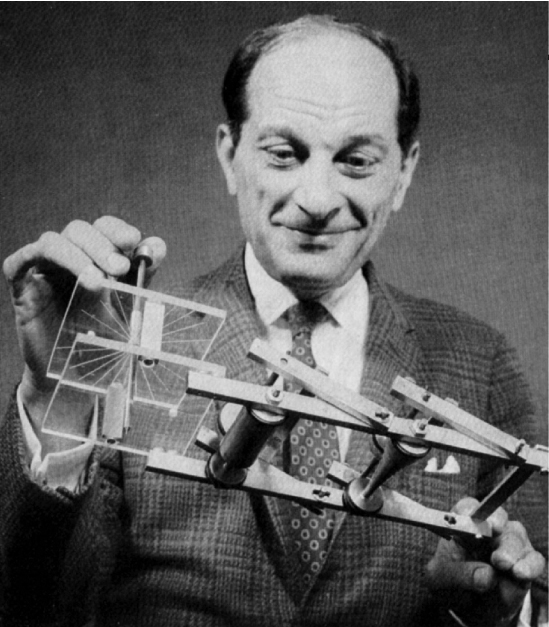
\includegraphics[width=0.9\columnwidth]{stanislaw.jpg}
    \end{column}
  \end{columns}
\end{frame}

\begin{frame}{História dos Métodos de Monte Carlo\footnote{para quem se interessou, a história se encontra em \textcite{eckhardtStanUlamJohn1987}}}
  \begin{columns}
    \begin{column}{0.8\textwidth}
      \begin{vfilleditems}
        \item A ideia do método veio enquanto jogava paciência durante sua
        recuperação de uma cirurgia, Ulam pensou em jogar centenas de jogos para
        estimar estatisticamente a probabilidade de um resultado bem-sucedido
        \item Ulam descreveu a ideia para John von Neumann em 1946
        \item \small Por ser secreto, o trabalho de von Neumann e Ulam exigia um codinome.
        Um colega de von Neumann e Ulam, Nicholas Metropolis, sugeriu usar o nome Monte Carlo,
        que se refere ao Casino Monte Carlo em Mônaco, onde o tio de Ulam (Michał Ulam)
        pedia dinheiro emprestado a parentes para jogar.
      \end{vfilleditems}
    \end{column}
    \begin{column}{0.2\textwidth}
      \centering
      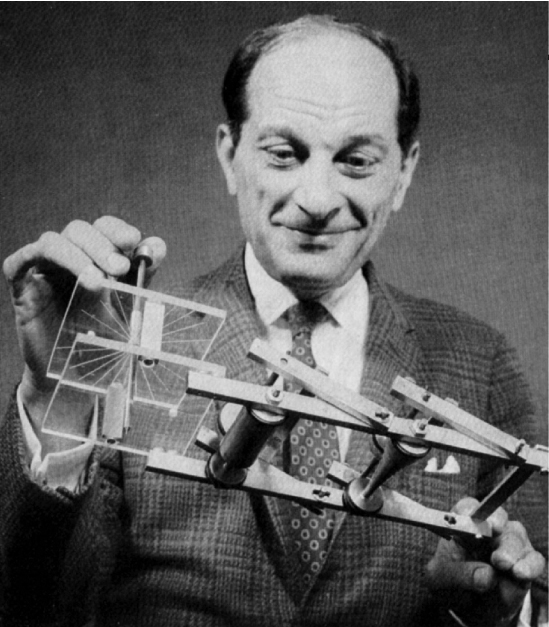
\includegraphics[width=0.9\columnwidth]{stanislaw.jpg}
    \end{column}
  \end{columns}
\end{frame}

\subsection{Por quê Precisamos de MCMC?}
\begin{frame}{Por quê Precisamos de MCMC?}
  A principal barreira computacional para estatística Bayesiana é o denominador
  $P(\text{data})$ da fórmula de Bayes:

  $$P(\theta \mid \text{data})=\frac{P(\theta) \cdot P(\text{data} \mid \theta)}{P(\text{data})}$$

  Em casos discretos podemos fazer o denominador virar a soma de todos os parâmetros
  usando a \textbf{regra da cadeia de probabilidade} (\textit{chain rule}):

  $$P(A,B \mid C)=P(A \mid B,C) \times P(B \mid C)$$

  Isto também é chamado de \textbf{marginalização}:

  $$P(\text{data})=\sum_{\theta} P(\text{data} \mid \theta) \times P(\theta)$$
\end{frame}

\begin{frame}{Por quê Precisamos de MCMC?}
  Porém no caso de valores contínuos o denominador $P(\text{data})$ vira uma integral
  bem grande e complicada de calcular:

  $$P(\text{data})=\int_{\theta} P(\text{data} \mid \theta) \times P(\theta)d \theta$$

  Em muitos casos essa integral vira \textit{intratável} (incalculável) e
  portanto devemos achar outras maneiras de calcular a probabilidade posterior
  $P(\theta \mid \text{data})$ de Bayes sem usar o denominador $P(\text{data})$.
  \vfill
  \Large \textbf{É aqui que entra Métodos de Monte Carlo!}
\end{frame}

\begin{frame}{Para quê serve o denominador $P(\text{data})$}
  Para normalizar a posterior com o intuito de torná-la uma distribuição
  probabilística válida. Isto quer dizer que a soma de todas as probabilidades
  dos eventos possíveis da distribuição devem ser iguais a $1$:
  \begin{vfilleditems}
    \item no caso de distribuição probabilística \textbf{discreta}:
    $$\sum_{\theta} P(\theta \mid \text{data}) = 1$$
    \item no caso de distribuição probabilística \textbf{contínua}:
    $$\int_{\theta} P(\theta \mid \text{data})d \theta = 1$$
  \end{vfilleditems}
\end{frame}

\begin{frame}{Se removermos o denominador de Bayes o que temos?}
  Ao removermos o denominador $(\text{data})$ temos que a posterior
  $P(\theta \mid \text{data})$ é \textbf{proporcional} à \textit{priori}
  multiplicada pela verossimilhança $P(\theta) \cdot P(\text{data} \mid \theta)$:

  $$P(\theta \mid \text{data}) \propto P(\theta) \cdot P(\text{data} \mid \theta)$$

\end{frame}

\subsubsection{Correntes Markov}
\begin{frame}{Método de Montecarlo com Correntes Markov -- (MCMC)}
  Aí que entra \textbf{Método Montecarlo com Correntes Markov}\footnote{do inglês
  \textit{Markov Chain Monte Carlo} (MCMC)}.
  \vfill
  MCMC é uma classe ampla de ferramentas computacionais para aproximação
  de integrais e geração de amostras de uma probabilidade posterior
  \parencite{brooksHandbookMarkovChain2011}.
  \vfill
  MCMC é usada quando não é possível coletar amostras de $\boldsymbol{\theta}$
  direto da distribuição probabilística posterior
  $P(\boldsymbol{\theta} \mid \text{data})$.
  Ao invés disso, nos coletamos amostras de maneira iterativa que a cada passo do
  processo nós esperamos que a distribuição da qual amostramos
  $P^*(\boldsymbol{\theta}^{(*)} \mid \text{data})$
  se torna cada vez mais similar à posterior $P(\boldsymbol{\theta} \mid \text{data})$.
  \vfill
  Tudo isso é para \textbf{eliminar o cálculo} (muitas vezes impossível) do \textbf{denominador} $P(\text{data})$.
\end{frame}

\begin{frame}{Correntes Markov}
  \begin{columns}
    \begin{column}{0.8\textwidth}
      \begin{vfilleditems}
        \item A ideia é \textbf{definir uma corrente Markov ergódica}
        (quer dizer que há uma distribuição estacionária única)
        dos quais o conjunto de estados possíveis é o espaço amostral e a
        distribuição estacionária é a distribuição a ser \textit{aproximada} (ou \textit{amostrada}).
        \item Seja $X_0, X_1, \dots, X_n$ uma simulação da corrente.
        A corrente Markov \textbf{converge à distribuição estacionária de qualquer
        estado inicial} $X_0$ após um \textbf{número suficiente grande de iterações} $r$,
        a distribuição do estado $X_r$ estará similar à distribuição estacionária,
        então podemos usá-la com amostra.
      \end{vfilleditems}
    \end{column}
    \begin{column}{0.2\textwidth}
      \centering
      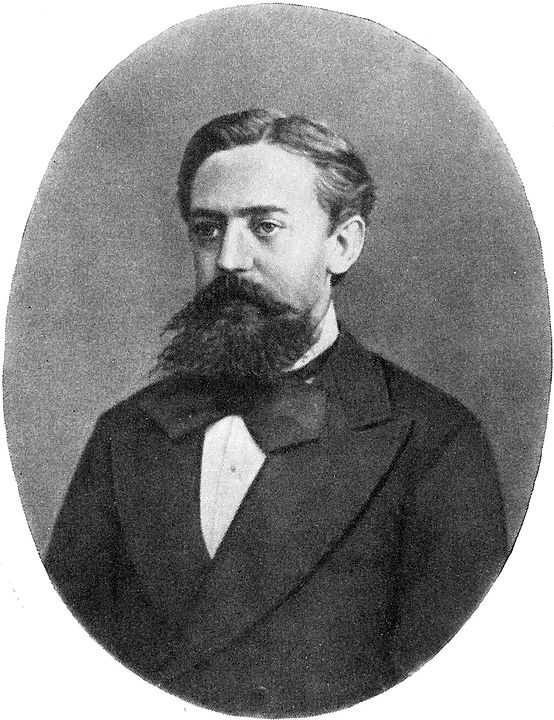
\includegraphics[width=0.9\columnwidth]{andrei_markov.jpg}
    \end{column}
  \end{columns}
\end{frame}

\begin{frame}{Correntes Markov}
  \begin{columns}
    \begin{column}{0.8\textwidth}
      \begin{vfilleditems}
        \item As correntes Markov possuem uma propriedade que a distribuição probabilística
        do próximo estado depende \textbf{apenas do estado atual e não na sequência
        de eventos que precederam}:
        $P(X_{n+1}=x \mid X_{0},X_{1},X_{2},\ldots ,X_{n}) = P(X_{n+1}=x \mid X_{n})$.
        Essa propriedade é chamada de \textbf{Markoviana}.
        \item Similarmente, repetindo esse argumento com $X_r$ como o ponto inicial,
        podemos usar $X_{2r}$ como amostra, e assim por diante.
        Podemos então usar a sequência de estados $X_r, X_{2r}, X_{3r}, \dots$
        como quase \textbf{amostras independentes} da distribuição estacionária da
        corrente Markov.
      \end{vfilleditems}
    \end{column}
    \begin{column}{0.2\textwidth}
      \centering
      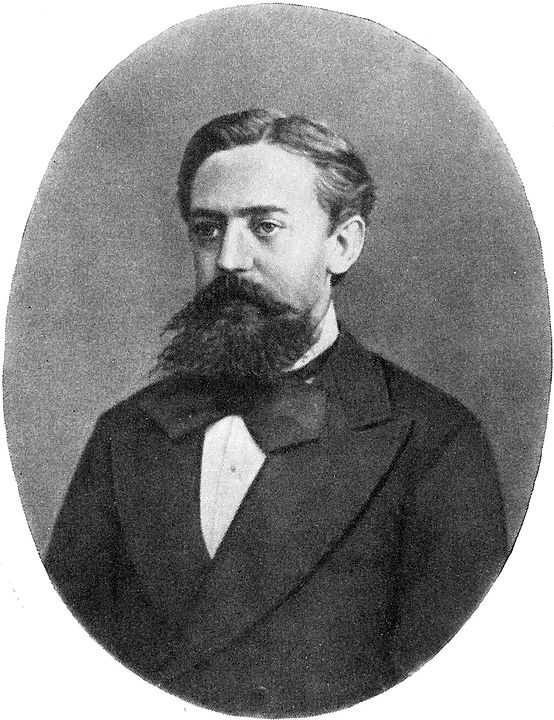
\includegraphics[width=0.9\columnwidth]{andrei_markov.jpg}
    \end{column}
  \end{columns}
\end{frame}

% Idea taken from http://steventhornton.ca/blog/markov-chains-in-latex.html
\begin{frame}{Exemplo de Corrente Markov}
  \centering
  \begin{tikzpicture}
    % Add the states
    \node[state,
    text=yellow,
    minimum size=2cm,
    thick
    ]
    (s) {Sol};
    \node[state,
    right=3cm of s,
    text=blue!30!white,
    minimum size=2cm,
    thick
    ]
    (r) {Chuva};

% Connect the states with arrows
\draw[every loop,
    auto=right,
    line width=1mm,
    >=latex]
  (s) edge[bend right, auto=left]  node {0.6} (r)
  (r) edge[bend right, auto=right] node {0.7} (s)
  (s) edge[loop above]             node {0.4} (s)
  (r) edge[loop above]             node {0.3} (r);
\end{tikzpicture}
\end{frame}

\begin{frame}{Correntes Markov}
  A eficácia dessa abordagem depende em:

  \begin{vfilleditems}
    \item \textbf{o quão grande $r$ deve ser} para garantir uma \textbf{amostra adequadamente boa}
    \item \textbf{poder computacional} requerido para cada iteração da corrente Markov.
  \end{vfilleditems}

  \vfill
  \footnotesize
  Além disso, é costumeiro descartarmos as primeiras iterações do algoritmo pois
  elas costumam não ser representativas da distribuição a ser aproximada.
  Nas iterações iniciais de algoritmos MCMC geralmente a corrente Markov
  está em um processo de aquecimento\footnote{Algumas referências chamam esse processo de \textit{burnin}}
  (\textit{warm-up}) e seu estado está bem distante do ideal para começarmos uma amostragem
  fidedigna.
  \vfill
  Geralmente, recomenda-se que se descarte metade das iterações \parencite{gelmanBasicsMarkovChain2013}.
\end{frame}

\subsection{Algoritmos de MCMC}
\begin{frame}{Algoritmos de MCMC}
  Temos \textbf{MUITOS} algoritmos de MCMC\footnote{Veja a \href{https://en.wikipedia.org/wiki/Markov_chain_Monte_Carlo}{página da Wikipedia para uma listagem completa}}
  Mas aqui vamos cobrir duas classes de algoritmos MCMC:
  \begin{vfilleditems}
    \item Metropolis-Hastings \parencite{metropolisEquationStateCalculations1953, hastingsMonteCarloSampling1970}

    \item Hamiltonian Monte Carlo\footnote{às vezes chamado de \textit{Hybrid Monte Carlo}, especialmente na literatura de Física} \parencite{neal2011mcmc, betancourtConceptualIntroductionHamiltonian2017}
  \end{vfilleditems}
\end{frame}

\begin{frame}{Classe de Algoritmos MCMC -- Metropolis-Hastings}
  Os primeiros algoritmos de MCMC. Usam uma regra de aceitação/rejeição das
  propostas. Caracterizados por propostas oriundas de um passeio aleatório\footnote{\textit{random walk}}
  no espaço amostral. O algoritmo de \textbf{Gibbs} pode ser visto como um
  \textbf{caso especial} do algoritmo de MH porque
  todas as propostas são aceitas \parencite{gelmanIterativeNonIterativeSimulation1992}
  \vfill
  Assintoticamente, possuem uma taxa de aceitação de 23.4\% e o custo de cada iteração é
  $\mathcal{O}(d)$, na qual $d$ é a dimensão do espaço amostral \parencite{beskosOptimalTuningHybrid2013}.
\end{frame}

\begin{frame}{Classe de Algortimos MCMC -- Hamiltonian Monte Carlo}
  Os algoritmos MCMC mais eficientes na atualidade. Tenta evitar o comportamento
  de passeio aleatório introduzindo um vetor de momento auxiliar e
  implementando dinâmicas Hamiltonianas. As propostas são "guiadas"~
  para regiões de maior densidade do espaço amostral. Isso faz com que HMC seja
  \textbf{ordens de magnitude mais eficiente que MH e Gibbs}.
  \vfill
  Assintoticamente, possuem uma taxa de aceitação de 65.1\% e o custo de cada iteração é
  $\mathcal{O}(d^{\frac{1}{4}})$, na qual $d$ é a dimensão do espaço amostral \parencite{beskosOptimalTuningHybrid2013}.
\end{frame}

\subsubsection{Metropolis}
\begin{frame}{Algoritmo de Metropolis}
  \begin{columns}
    \begin{column}{0.8\textwidth}
      O primeiro algoritmo MCMC amplamente utilizado para gerar amostras de
      correntes Markov foi originário na física na década de 1950 e chama-se Metropolis
      \parencite{metropolisEquationStateCalculations1953} em homenagem ao primeiro
      autor \href{https://en.wikipedia.org/wiki/Nicholas_Metropolis}{Nicholas Metropolis}.
      \vfill
      Em síntese, o algoritmo de Metropolis é uma adaptação de um passeio aleatório
      com uma regra de aceitação/rejeição para convergir à distribuição-alvo.
      \vfill
      O algorimo de Metropolis usa uma \textbf{distribuição de propostas}
      $J_t(\boldsymbol{\theta}^{(*)})$
      para definir próximos valores da distribuição
      $P^*(\boldsymbol{\theta}^{(*)} \mid \text{data})$.
      Essa distribuição deve ser simétrica:
      $$
      J_t (\boldsymbol{\theta}^{(*)} \mid \boldsymbol{\theta}^{(t-1)}) = J_t(\boldsymbol{\theta}^{(t-1)} \mid \boldsymbol{\theta}^{(*)})
      $$
    \end{column}
    \begin{column}{0.2\textwidth}
      \centering
      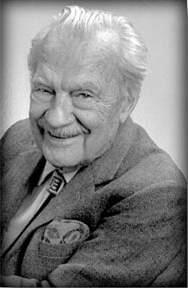
\includegraphics[width=0.9\columnwidth]{nicholas_metropolis.png}
    \end{column}
  \end{columns}
\end{frame}

\begin{frame}{Algoritmo de Metropolis}
  A essência do algoritmo é um passeio aleatório pelo espaço amostral dos parâmetros,
  onde a probabilidade da corrente Markov mudar de estado é definida como:

  $$
  P_{\text{mudar}} = \min\left({\frac{P (\boldsymbol{\theta}_{\text{proposto}})}{P (\boldsymbol{\theta}_{\text{atual}})}},1\right).
  $$

  Isso quer dizer a corrente Markov somente mudará para um novo estado em duas condições:
  \begin{vfilleditems}
    \small
    \item \small Quando a probabilidade dos parâmetros propostos pelo passeio aleatório
    $P(\boldsymbol{\theta}_{\text{proposto}})$ é \textbf{\textcolor{blue}{maior}}
    que a probabilidade dos parâmetros do estado atual
    $P(\boldsymbol{\theta}_{\text{atual}})$, mudamos com 100\% de probabilidade.

    \item \small Quando a probabilidade dos parâmetros propostos pelo passeio aleatório
    $P(\boldsymbol{\theta}_{\text{proposto}})$ é \textbf{\textcolor{red}{menor}}
    que a probabilidade dos parâmetros do estado atual
    $P(\boldsymbol{\theta}_{\text{atual}})$, mudamos com probabilidade igual a
    proporção dessa diferença.
  \end{vfilleditems}
\end{frame}

\begin{frame}[fragile]{Algoritmo de Metropolis}
    \SetAlCapFnt{\normalsize}
    \SetAlCapNameFnt{\normalsize}
    \begin{algorithm}[H]
    \DontPrintSemicolon
    \SetAlgoNoEnd
    \SetAlgoLined
    Defina um ponto inicial $\boldsymbol{\theta}^{(0)} \in \mathbb{R}^p$ do qual $P\left(\boldsymbol{\theta}^{(0)} \mid \boldsymbol{y} \right) > 0$\;
     \Para{$t = 1, 2, \dots$}{
      Amostra uma proposta $\boldsymbol{\theta}^{(*)}$ de uma distribuição de propostas no tempo $t$, $J_t \left(\boldsymbol{\theta}^{(*)} \mid \boldsymbol{\theta}^{(t-1)} \right)$\;
      Como regra de aceitação/rejeição calcule a proporção das probabilidades:
      $r = \frac{P\left(\boldsymbol{\theta}^{(*)}  \mid \boldsymbol{y} \right)}{P\left(\boldsymbol{\theta}^{(t-1)} \mid \boldsymbol{y} \right)}$\;
      Designe:
      $
        \boldsymbol{\theta}^{(t)} =
          \begin{cases}
          \boldsymbol{\theta}^{(*)} & \text{com probabilidade $\min(r,1)$}\\
          \boldsymbol{\theta}^{(t-1)} & \text{caso contrário}
        \end{cases}
      $\;
     }
     \caption{Metropolis}
    \end{algorithm}
\end{frame}

\begin{frame}{Intuição Visual de Metropolis}
\centering
    \begin{tikzpicture}
        \begin{axis}[every axis plot, line width=2pt,
            ylabel=PDF,
            domain=-4:4,samples=200,
            ymax = 0.6, ytick={0, 0.2, 0.4},
            axis x line*=bottom, % no box around the plot, only x and y axis
            axis y line*=left, % the * suppresses the arrow tips
            enlargelimits=true,
            ] % extend the axes a bit

            \addplot [blue] {gaussian(0, 1)};
            \node[inner sep=0pt] (hikerlower) at (-2,0.13){\Strichmaxerl[2pt]};
            \node[inner sep=0pt] (hikerupper) at (0,0.5){\Strichmaxerl[2pt]};
            \node[inner sep=0pt] (hikerlower2) at (2,0.13){\Strichmaxerl[2pt]};
            \draw[->, red, line width=2pt] (hikerlower) to [out=90,in=135] node[above left] {\large$P=1$} (hikerupper);
            \draw[->, yellow, line width=2pt] (hikerupper) to [out=45,in=135] node[right] {\large$P\approx\frac{0.1}{0.4}\approx\frac{1}{4}$} (hikerlower2);
        \end{axis}
        \end{tikzpicture}

\end{frame}

\subsubsection{Metropolis-Hastings}
\begin{frame}{Algoritmo de Metropolis}
  \begin{columns}
    \begin{column}{0.8\textwidth}
      Na década de 1970, surgiu um generalização do algoritmo de Metropolis
      que \textbf{não} necessita que as distribuições de proposta sejam simétricas:
      $$
      J_t (\boldsymbol{\theta}^{(*)} \mid \boldsymbol{\theta}^{(t-1)}) \neq J_t(\boldsymbol{\theta}^{(t-1)} \mid \boldsymbol{\theta}^{(*)})
      $$
      A generalização foi proposta por \href{https://en.wikipedia.org/wiki/W._K._Hastings}{Wilfred Keith Hastings}
      \parencite{hastingsMonteCarloSampling1970} e chama-se algoritmo
      de \textbf{Metropolis-Hastings}.
    \end{column}
    \begin{column}{0.2\textwidth}
      \centering
      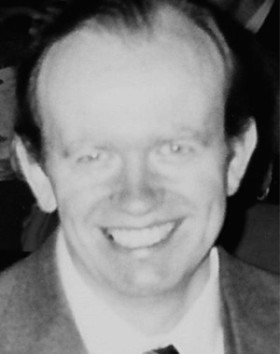
\includegraphics[width=0.9\columnwidth]{hastings.jpg}
    \end{column}
  \end{columns}
\end{frame}

\begin{frame}[fragile]{Algoritmo de Metropolis - Hastings}
    \SetAlCapFnt{\normalsize}
    \SetAlCapNameFnt{\normalsize}
    \small
    \begin{algorithm}[H]
    \DontPrintSemicolon
    \SetAlgoNoEnd
    \SetAlgoLined
    Defina um ponto inicial $\boldsymbol{\theta}^{(0)} \in \mathbb{R}^p$ do qual $P\left(\boldsymbol{\theta}^{(0)} \mid \boldsymbol{y} \right) > 0$\;
     \Para{$t = 1, 2, \dots$}{
      Amostra uma proposta $\boldsymbol{\theta}^{(*)}$ de uma distribuição de propostas no tempo $t$, $J_t \left(\boldsymbol{\theta}^{(*)} \mid \boldsymbol{\theta}^{(t-1)} \right)$\;
      Como regra de aceitação/rejeição calcule a proporção das probabilidades:
      $r = \frac{\frac{P \left(\boldsymbol{\theta}^{(*)} \mid \boldsymbol{y} \right)}{J_t \left(\boldsymbol{\theta}^{(*)} \mid \boldsymbol{\theta}^{(t-1)} \right)}}{\frac{P \left(\boldsymbol{\theta}^{(t-1)} \mid \boldsymbol{y} \right)}{J_t \left(\boldsymbol{\theta}^{(t-1)} \mid \boldsymbol{\theta}^{(*)} \right)}}$\;
      Designe:
      $
        \boldsymbol{\theta}^{(t)} =
          \begin{cases}
          \boldsymbol{\theta}^{(*)} & \text{com probabilidade $\min(r,1)$}\\
          \boldsymbol{\theta}^{(t-1)} & \text{caso contrário}
        \end{cases}
      $\;
     }
     \caption{Metropolis-Hastings}
    \end{algorithm}
\end{frame}

\begin{frame}{Animação Metropolis\footnote{veja Metropolis em ação no \href{https://chi-feng.github.io/mcmc-demo/app.html?algorithm=RandomWalkMH&target=banana}{\texttt{chi-feng/mcmc-demo}}}}
  \centering
  \includemedia[
    width=\linewidth,
    height=0.3\linewidth,
    addresource=rwmh.m4v,
    transparent,
    activate=pageopen,
    passcontext,  %show VPlayer's right-click menu
    flashvars={
      source=rwmh.m4v
      &loop=true
      &scaleMode=stretch
    }
  ]{Animação Metropolis}{http://mirrors.ctan.org/macros/latex/contrib/media9/players/VPlayer.swf}
\end{frame}

\subsubsection{Limitações dos Algoritmos Metropolis}
\begin{frame}{Limitações dos Algoritmos Metropolis}
  As limitações do algoritmo de Metropolis-Hastings são principalmente
  \textbf{computacionais}:
  \begin{vfilleditems}
    \item Com propostas geradas aleatoriamente, geralmente leva um grande número de
    iterações para entrar em áreas de densidade posterior mais alta (mais provável).

    \item Mesmo algoritmos de Metropolis-Hastings eficientes às vezes aceitam menos de
    25\% das propostas \parencite{robertsWeakConvergenceOptimal1997, beskosOptimalTuningHybrid2013}.

    \item Em situações dimensionais mais baixas, o poder computacional aumentado pode compensar a eficiência mais baixa até certo ponto.
    Mas em situações de modelagem de dimensões mais altas e mais complexas, computadores maiores
    e mais rápidos sozinhos raramente são suficientes para superar o desafio.
  \end{vfilleditems}
\end{frame}

\subsubsection{Gibbs}
\begin{frame}{Algoritmo de Gibbs}
  \begin{columns}
    \begin{column}{0.8\textwidth}
      Para contornar o problema de baixa taxa de aceitação dos algoritmos de Metropolis
      foi desenvolvido o algoritmo de Gibbs que
      \textbf{não possui uma regra de aceitação/rejeição}
      para a mudança de estado da corrente Markov:
      \textbf{Todas as propostas são aceitas}!
      \vfill
      O algoritmo de Gibbs teve ideia original concebida pelo físico Josiah Willard Gibbs
      em referência a uma analogia entre um algoritmo de amostragem e a
      física estatística (\textit{statistical physics} um ramo da física que tem sua
      base em mecânica estatística, \textit{statistical mechanics}).
      O algoritmo foi descrito pelos irmãos Stuart e Donald Geman em 1984
      \parencite{gemanStochasticRelaxationGibbs1984}, cerca de oito décadas após
      a morte de Gibbs.
    \end{column}
    \begin{column}{0.2\textwidth}
      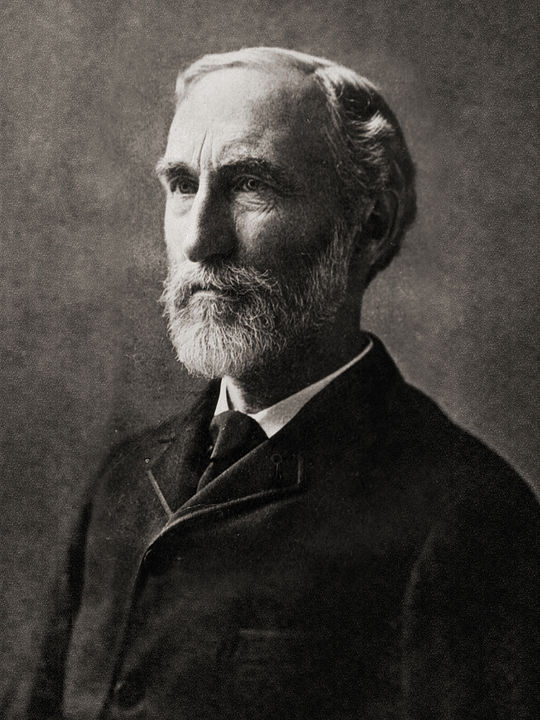
\includegraphics[width=0.9\columnwidth]{josiah_gibbs.jpg}
    \end{column}
  \end{columns}
\end{frame}

\begin{frame}{Algoritmo de Gibbs}
  O algoritmo de Gibbs é muito útil em espaços amostrais multidimensionais\footnote{
  no qual há bem mais que 2 parâmetros a serem amostrados da probabilidade posterior}.
  Também é conhecido como amostragem condicional alternativa
  (\textit{alternating conditional sampling}), pois amostramos sempre um parâmetro
  \textbf{condicionado} à probabilidade dos outros parâmetros do modelo.
  \vfill
  O algoritmo de Gibbs pode ser visto como um \textbf{caso especial} do algoritmo
  de Metropolis-Hastings porque todas as propostas são aceitas
  \parencite{gelmanIterativeNonIterativeSimulation1992}.
  \vfill
  A essência do algoritmo de Gibbs é a amostragem de parâmetros condicionada à outros parâmetros:
  $$P(\theta_1 \mid \theta_2, \dots \theta_p)$$
\end{frame}

\begin{frame}[fragile]{Algoritmo de Gibbs}
    \SetAlCapFnt{\normalsize}
    \SetAlCapNameFnt{\normalsize}
    \begin{algorithm}[H]
    \DontPrintSemicolon
    \SetAlgoNoEnd
    \SetAlgoLined
    Defina um ponto inicial $\boldsymbol{\theta}^{(0)} \in \mathbb{R}^p$ do qual $P\left(\boldsymbol{\theta}^{(0)} \mid \boldsymbol{y} \right) > 0$\;
     \Para{$t = 1, 2, \dots$}{
      Designe:
      $ \boldsymbol{\theta}^{(t)} =
        \begin{cases}
        \theta^{(t)}_1 &\sim P \left(\theta_1 \mid \theta^{(0)}_2, \dots, \theta^{(0)}_p \right) \\
        \theta^{(t)}_2 &\sim P \left(\theta_2 \mid \theta^{(t-1)}_1, \dots, \theta^{(0)}_p \right) \\
        &\vdots \\
        \theta^{(t)}_p &\sim P \left(\theta_p \mid \theta^{(t-1)}_1, \dots, \theta^{(t-1)}_{p-1} \right)
     \end{cases}
      $\;
     }
     \caption{Gibbs}
    \end{algorithm}
\end{frame}

\begin{frame}{Animação Gibbs\footnote{Veja Gibbs em ação no \href{https://chi-feng.github.io/mcmc-demo/app.html?algorithm=GibbsSampling&target=banana}{\texttt{chi-feng/mcmc-demo}}}}
  \centering
  \includemedia[
    width=\linewidth,
    height=0.3\linewidth,
    addresource=gibbs.m4v,
    transparent,
    activate=pageopen,
    passcontext,  %show VPlayer's right-click menu
    flashvars={
      source=gibbs.m4v
      &loop=true
      &scaleMode=stretch
    }
  ]{Animação Gibbs}{http://mirrors.ctan.org/macros/latex/contrib/media9/players/VPlayer.swf}
\end{frame}

\subsubsection{Limitações do Algoritmo de Gibbs}
\begin{frame}{Limitações do Algoritmo de Gibbs}
  A principal limitação do algoritmo de Gibbs é com relação a
  \textbf{amostragem condicional alternativa}:
  \begin{vfilleditems}
    \item Em Metropolis temos propostas aleatórias
    de uma distribuição de propostas na qual amostramos cada parâmetro
    \textbf{incondicionalmente} à outros parâmetros e de maneira \textbf{simultânea} usando a
    probabilidade conjunta desses parâmetros. As mudanças de estado da corrente
    Markov são então executadas \textbf{multidimensionalmente}.
    Isto provoca movimentos "\textbf{diagonais}"~multidimensionais.

    \item No caso do algoritmo de Gibbs essa movimentação se dá apenas em um
    único parâmetro, pois amostramos \textbf{sequencialmente} e
    \textbf{condicionalmente} à outros parâmetros.
    Isto provoca movimentos \textbf{horizontais/verticais} unidimensionais,
    mas nunca movimentos diagonais multidimensionais.
  \end{vfilleditems}
\end{frame}

\subsubsection{Hamiltonian Monte Carlo (HMC)}
\begin{frame}{Classe de Algoritmos MCMC - Hamiltoninan Monte Carlo (HMC)}
  \begin{columns}
    \begin{column}{0.8\textwidth}
      Os problemas de baixas taxas de aceitação de propostas das técnicas de
      Metropolis e do desempenho baixo do algoritmo de Gibbs em problemas
      multidimensionais nas quais a geometria da posterior é complexa
      fizeram com que surgisse uma nova técnica MCMC usando dinâmica Hamiltoniana
      (em homenagem ao físico irlandês
      \href{https://en.wikipedia.org/wiki/William_Rowan_Hamilton}{William Rowan Hamilton}.
    \end{column}
    \begin{column}{0.2\textwidth}
      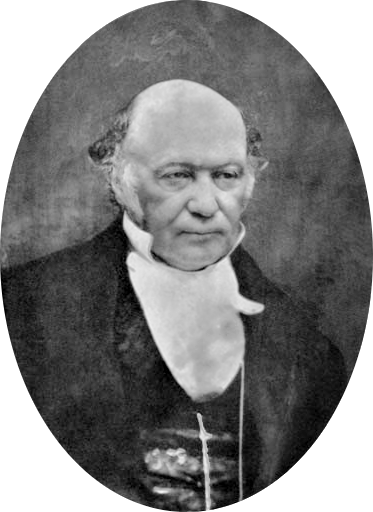
\includegraphics[width=0.9\columnwidth]{hamilton.png}
    \end{column}
  \end{columns}
\end{frame}

\begin{frame}{Algoritmo de HMC}
  O HMC é uma adaptação da técnica de Metropolis e emprega um esquema guiado de
  geração de novas proposta: isso melhora a taxa de aceitação de propostas e,
  consequentemente, a eficiência.
  \vfill
  Mais especificamente, o HMC usa o gradiente do log da posterior para direcionar
  a cadeia de Markov para regiões de maior densidade posterior,
  onde a maioria das amostras são coletadas.
  $$
  \frac{d \log P(\boldsymbol{\theta} \mid \boldsymbol{y})}{d \theta}
  $$
  Como resultado, uma corrente Markov com o algoritmo HMC bem ajustada aceitará
  propostas em uma taxa muito mais alta do que o algoritmo Metropolis tradicional
  \parencite{robertsWeakConvergenceOptimal1997, beskosOptimalTuningHybrid2013}.
\end{frame}

\begin{frame}{História do Algoritmo de HMC}
  HMC foi inicialmente descrito na literatura de física\footnote{que chamaram de \textit{"Hybrid"~Monte Carlo} -- HMC}
  \parencite{duaneHybridMonteCarlo1987}.
  \vfill
  Logo depois, HMC foi aplicado a problemas estatísticos por
  \textcite{nealImprovedAcceptanceProcedure1994} que chamou de \textit{Hamiltonean Monte Carlo}
  -- HMC).
  \vfill
  Para uma discussão aprofundada (que não é o foco deste conteúdo) de HMC eu recomendo
  \textcite{neal2011mcmc} e \textcite{betancourtConceptualIntroductionHamiltonian2017}.
\end{frame}

\begin{frame}{O que muda com HMC?}
  HMC usa dinâmica Hamiltoniana aplicada para partículas explorando de maneira mais
  eficiente a geometria de uma probabilidade posterior.
  \vfill
  Além de explorar melhor a geometria da posterior e tolerar geometrias complexas,
  HMC é muito mais eficiente que Metropolis e não sofre do problema de correlação
  dos parâmetros que Gibbs.
\end{frame}

\begin{frame}{Intuição por trás do Algoritmo de HMC}
  \small
  Para cada componente $\theta_j$, o HMC adiciona uma variável de momento
  $\phi_j$. A densidade posterior $P(\boldsymbol{\theta} \mid y)$ é incrementada
  por uma distribuição independente $P(\boldsymbol{\phi})$ dos momentos,
  definindo assim uma distribuição conjunta:
  $$
  P(\boldsymbol{\theta}, \boldsymbol{\phi} \mid y) = P(\boldsymbol{\phi}) \cdot P(\boldsymbol{\theta} \mid y)
  $$
  \small
  O HMC usa uma distribuição de propostas que muda dependendo do estado atual na
  corrente Markov. O HMC descobre a direção em que a distribuição posterior aumenta,
  chamada de \textit{gradiente}, e distorce a distribuição de propostas em
  direção ao \textit{gradiente}.
  \vfill
  A probabilidade da corrente Markov mudar de estado no algoritmo HMC é definida como:
  $$
  P_{\text{mudar}} = \min\left({\frac{P(\boldsymbol{\theta}_{\text{proposto}}) \cdot P(\boldsymbol{\phi}_{\text{proposto}})}{P(\boldsymbol{\theta}_{\text{atual}})\cdot P(\boldsymbol{\phi}_{\text{atual}})}}, 1\right)
  $$
\end{frame}

\begin{frame}{Distribuição dos Momentos -- $P(\boldsymbol{\phi})$}
  Normalmente damos a $\boldsymbol{\phi}$ uma distribuição normal multivariada
  com média 0 e covariância de $\mathbf{M}$,
  uma "matriz de massa".
  \vfill
  Para mantêr as coisas um pouco mais simples, usamos uma matriz de massa diagonal
  $\mathbf{M}$. Isso faz com que os componentes de $\boldsymbol{\phi}$ sejam
  independentes com
  $$\phi_j \sim \text{Normal}(0, M_{jj})$$
\end{frame}

\begin{frame}[fragile]{Algoritmo de HMC}
    \SetAlCapFnt{\normalsize}
    \SetAlCapNameFnt{\normalsize}
    \begin{algorithm}[H]
    \DontPrintSemicolon
    \SetAlgoNoEnd
    \SetAlgoLined
    \footnotesize
    Defina um ponto inicial $\boldsymbol{\theta}^{(0)} \in \mathbb{R}^p$ do qual $P\left(\boldsymbol{\theta}^{(0)} \mid \boldsymbol{y} \right) > 0$\;
    Amostre $\boldsymbol{\phi}$ de uma $\text{Normal}(\mathbf{0},\mathbf{M})$\;
    Simultaneamente amostre $\boldsymbol{\theta}^{(*)}$ e $\boldsymbol{\phi}$ com $L$ passos e tamanho de passo $\epsilon$.\;
    Defina o valor atual $\boldsymbol{\theta}$ como valor proposto $\boldsymbol{\theta}^{(*)}$:
    $\boldsymbol{\theta}^{(*)} \leftarrow \boldsymbol{\theta}$\;
    \Para{$1, 2, \dots, L$}{
     Use o gradiente do $\log$ da posterior de $\boldsymbol{\theta}^{(*)}$ para produzir um meio-passo de $\boldsymbol{\phi}$:
     $\boldsymbol{\phi} \leftarrow \boldsymbol{\phi} + \frac{1}{2} \epsilon \frac{d \log P(\boldsymbol{\theta}^{(*)} \mid \boldsymbol{y})}{d \theta}$\;
     Use $\boldsymbol{\phi}$ para atualizar $\boldsymbol{\theta}^{(*)}$:
     $\boldsymbol{\theta}^{(*)} \leftarrow \boldsymbol{\theta}^{(*)} + \epsilon \mathbf{M}^{-1} \boldsymbol{\phi}$\;
     Novamente use o gradiente de $\boldsymbol{\theta}$ para produzir um meio-passo de $\boldsymbol{\phi}$:
     $\boldsymbol{\phi} \leftarrow \boldsymbol{\phi} + \frac{1}{2} \epsilon \frac{d \log P(\boldsymbol{\theta}^{(*)} \mid \boldsymbol{y})}{d \theta}$\;
    }
    Como regra de aceitação/rejeição calcule:
    $r = \frac{P \left(\boldsymbol{\theta}^{(*)} \mid \boldsymbol{y} \right) P \left(\boldsymbol{\phi}^{(*)} \right)}{P \left(\boldsymbol{\theta}^{(t-1)} \mid \boldsymbol{y} \right) P \left(\boldsymbol{\phi}^{(t-1)} \right)}$\;
    Designe:
      $
        \boldsymbol{\theta}^{(t)} =
          \begin{cases}
          \boldsymbol{\theta}^{(*)} & \text{com probabilidade $\min(r,1)$}\\
          \boldsymbol{\theta}^{(t-1)} & \text{caso contrário}
        \end{cases}
      $\;
    \caption{Hamiltonian Monte Carlo (HMC)}
    \end{algorithm}
\end{frame}

\begin{frame}{Animação HMC\footnote{Veja HMC em ação no \href{https://chi-feng.github.io/mcmc-demo/app.html?algorithm=HamiltonianHMC&target=banana}{\texttt{chi-feng/mcmc-demo}}}}
  \includemedia[
    width=\linewidth,
    height=0.3\linewidth,
    addresource=hmc.m4v,
    transparent,
    noplaybutton,
    activate=pageopen,
    passcontext,  %show VPlayer's right-click menu
    flashvars={
      source=hmc.m4v
      &loop=true
      &scaleMode=stretch
    }
  ]{Animação HMC}{http://mirrors.ctan.org/macros/latex/contrib/media9/players/VPlayer.swf}
\end{frame}

\begin{frame}{Um interlúdio de Integrador Numéricos}
  No campo das equações diferenciais ordinais temos a ideia de discretizar um
  sistema de equações diferenciais ordinais ao aplicar um pequeno passo $\epsilon$\footnote{algumas vezes também chamado de $h$}.
  Tais abordagem são chamadas de \textbf{integradores numéricos} e comportam uma
  \textbf{ampla classe} de ferramentas.
  \vfill
  O mais famoso e simples desses integradores numéricos é o método de Euler. No qual
  usa-se um tamamho de passo $\epsilon$ para calcular a solução numérica do estado
  em um futuro tempo $t$ a partir de condições iniciais específicas.
\end{frame}

\begin{frame}{Um interlúdio de Integrador Numéricos}
  \begin{columns}
    \begin{column}{0.6\textwidth}
      O problema é que o método de Euler quando aplicado para dinâmicas Hamiltonianas
      é que ele não preserva o volume. Uma das propriedades fundamentais das dinâmicas
      Hamiltonianas é que elas presevam volume, um resultado chamado de Teorema de
      Liouville. Isto faz com que o método de Euler seja uma péssima escolha como
      integrador numérico de um algoritmo HMC.
    \end{column}
    \begin{column}{0.4\textwidth}
      \begin{figure}
      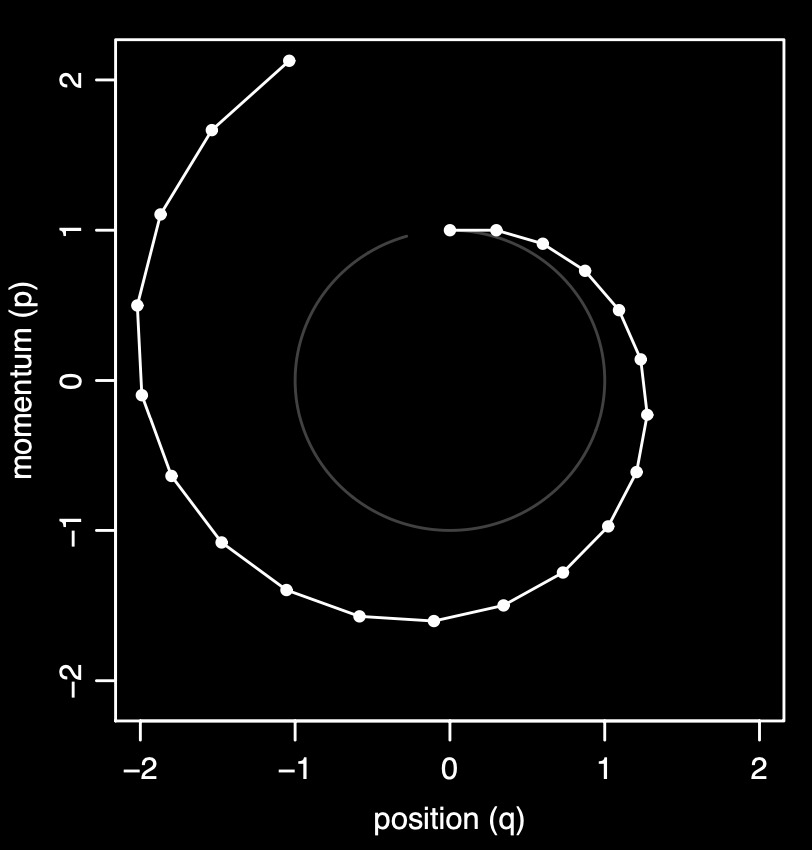
\includegraphics[width=0.8\columnwidth]{euler_0_3.jpg}
      \caption{Método de Euler num algoritmo HMC com $\epsilon = 0.3$ e $L = 20$}
      \end{figure}
    \end{column}
  \end{columns}
\end{frame}

\begin{frame}{Um interlúdio de Integrador Numéricos\footnote{Um excelente livro-texto
  para integradores numéricos e integradores simpléticos é
  \textcite{irseles2008numericalanalysis}}}
  \begin{columns}
    \begin{column}{0.6\textwidth}
      Para preservação de volumes precisamos usar um
      \textbf{integrador simplético}. Integradores simpléticos são no máximo
      de ordem 2 e precisam ser usados com um tamanho de passo $\epsilon$ constante.
      Um dos principais integradores numéricos simpléticos usado em dinânimcas
      Hamiltonianas é o integrador \textbf{Störmer–Verlet}, também conhecido
      como \textit{leapfrog}.
    \end{column}
    \begin{column}{0.4\textwidth}
      \begin{figure}
        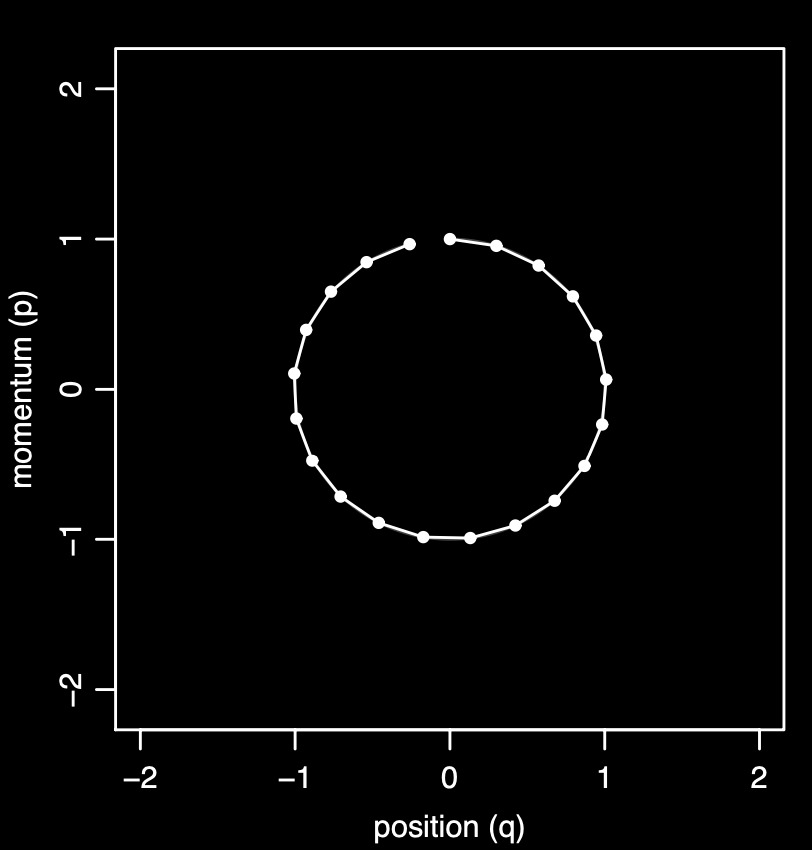
\includegraphics[width=0.8\columnwidth]{leapfrog_0_3.jpg}
        \caption{Integrador \textit{Leapfrog} num algoritmo HMC com $\epsilon = 0.3$ e $L = 20$}
        \end{figure}
    \end{column}
  \end{columns}
\end{frame}

\begin{frame}{Limitações do Algorito HMC}
  \begin{columns}
    \begin{column}{0.6\textwidth}
      Como vocês podem ver o algoritmo de HMC é muito sensível a escolhe da quantidade
      de passos $L$ e do tamanho do passo $\epsilon$. Em especial o integrador
      \textit{leapfrog} permite apenas um $\epsilon$ constante, portanto temos um
      equilíbrio delicado entre $L$ e $\epsilon$. Em  termos algorítmicos, $L$
      e $\epsilon$ são hiperparâmetros (tem que ser cuidadosamente ajustados).
    \end{column}
    \begin{column}{0.4\textwidth}
      \begin{figure}
        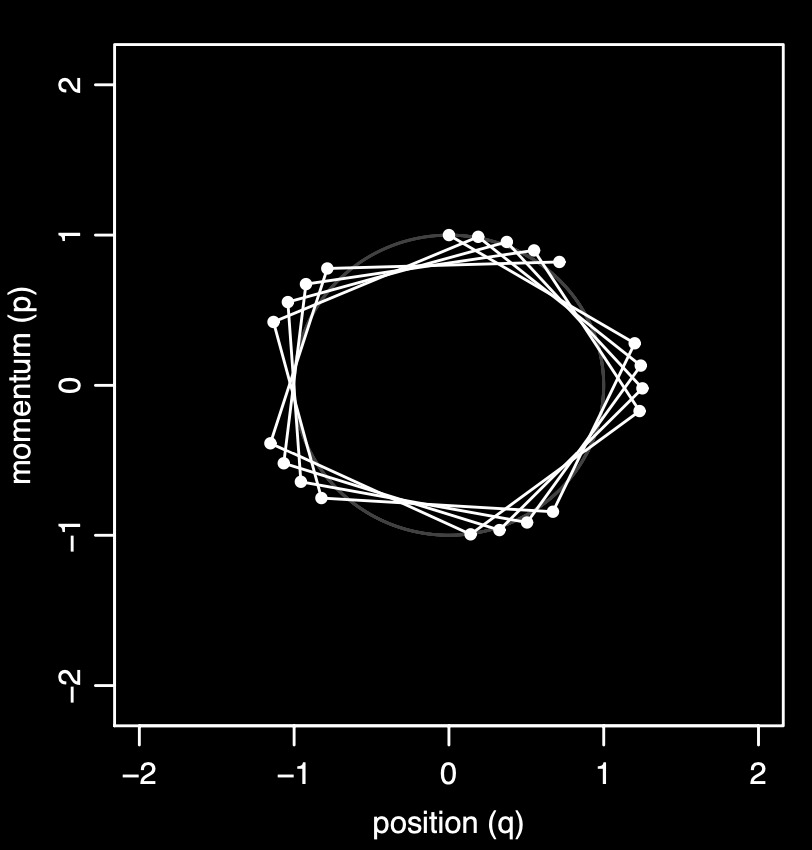
\includegraphics[width=0.8\columnwidth]{leapfrog_1_2.jpg}
        \caption{Integrador \textit{Leapfrog} num algoritmo HMC com $\epsilon = 1.2$ e $L = 20$}
        \end{figure}
    \end{column}
    \end{columns}
\end{frame}

\subsubsection{No-U-Turn-Sampler (NUTS)}
\begin{frame}{\textbf{N}o-\textbf{U}-\textbf{T}urn-\textbf{S}ampler (NUTS)}
  Em HMC, conseguimos ajustar o $\epsilon$ durante a execução do algoritmo. Mas, geralmente
  precisamos executar algumas vezes o amostrador HMC para ajustar o $L$.
  \vfill
  Aqui vem a ideia do \textbf{N}o-\textbf{U}-\textbf{T}urn-\textbf{S}ampler (NUTS)
  \parencite{hoffman2014no}.
  Não é preciso ajustar \textbf{nada} apenas "apertar"~o botão. Ele calcula automaticamente
  $\epsilon$ e $L$.
\end{frame}

\begin{frame}{\textbf{N}o-\textbf{U}-\textbf{T}urn-\textbf{S}ampler (NUTS)}
  Mais especificamente precisamos de um critério que informe que já simulamos as dinâmicas
  Hamiltonianas por "tempo suficiente". \textit{i.e.} simular as dinâmicas por mais tempo
  não aumentaria a distância entre a proposta $\boldsymbol{\theta}^{(*)}$ e o valor atual
  $\boldsymbol{\theta}$.
  \vfill
  NUTS então usa um critério baseado no produto interno entre os vetores do momento
  atual $\boldsymbol{\phi}$ e a diferença entre os vetores
  da proposta $\boldsymbol{\theta}^{(*)}$ e o valor atual $\boldsymbol{\theta}$,
  que é a derivativa com respeito ao tempo $t$ de metade da distância ao quadrado
  entre $\boldsymbol{\theta}$ e $\boldsymbol{\theta}^{(*)}$
  $$
  (\boldsymbol{\theta}^{(*)} - \boldsymbol{\theta}) \cdot \boldsymbol{\phi}
  = (\boldsymbol{\theta}^{(*)} - \boldsymbol{\theta}) \cdot \frac{d}{dt} (\boldsymbol{\theta}^{(*)} - \boldsymbol{\theta})
  = \frac{d}{dt} \frac{(\boldsymbol{\theta}^{(*)} - \boldsymbol{\theta}) \cdot (\boldsymbol{\theta}^{(*)} - \boldsymbol{\theta})}{2}
  $$
\end{frame}

\begin{frame}{\textbf{N}o-\textbf{U}-\textbf{T}urn-\textbf{S}ampler (NUTS)}
  Isso sugere um algorimo que não permite com que as propostas sejam guiadas de maneira
  infinita até que a distância entre a proposta $\boldsymbol{\theta}^{(*)}$ e o valor atual
  $\boldsymbol{\theta}$ seja menor que zero.
  \vfill
  Isto quer dizer que tal algoritmo não \textbf{permitirá meia-voltas} (\textit{u-turns}).
\end{frame}

\begin{frame}{\textbf{N}o-\textbf{U}-\textbf{T}urn-\textbf{S}ampler (NUTS)}
  NUTS usa o integrador \textit{leapfrog} para criar uma árvore binária da qual os nós-folha
  são as posições do momento $\boldsymbol{\phi}$ traçando tanto um caminho para frente
  ($t+1$) quanto para trás ($t-1$) em um tempo fictício em um determinado tempo $t$.
  O crescimento dos nós-folha são \textbf{interrompidos} quando é detectado meia-volta
  tanto para frente quanto para trás.
  \begin{figure}
    \centering
    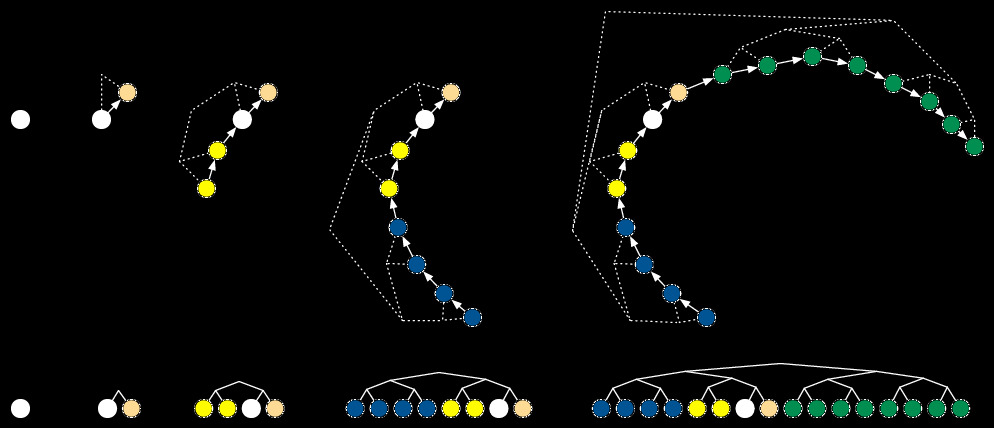
\includegraphics[width=0.6\textwidth]{nuts.jpg}
    \caption{NUTS crescendo nós-folha para frente}
  \end{figure}
\end{frame}

\begin{frame}{\textbf{N}o-\textbf{U}-\textbf{T}urn-\textbf{S}ampler (NUTS)}
  NUTS também um procedimento chamado \textit{Dual Averaging}
  \parencite{nesterov2009primal} para ajustar simultaneamente $\epsilon$ e $L$ ao
  considerar o produto $\epsilon \cdot L$.
  \vfill
  Tal ajuste é feito durante a fase de \textit{warmup} e os valores definidos de
  $\epsilon$ e $L$ são mantidos fixos durante a fase de amostragem.
\end{frame}

\begin{frame}{Algoritmo de NUTS}
    \SetAlCapFnt{\footnotesize}
    \SetAlCapNameFnt{\footnotesize}
    \begin{algorithm}[H]
    \DontPrintSemicolon
    \SetAlgoNoEnd
    \SetAlgoLined
    \fontsize{4.5pt}{6.5pt}\selectfont
    Defina um ponto inicial $\boldsymbol{\theta}^{(0)} \in \mathbb{R}^p$ do qual $P\left(\boldsymbol{\theta}^{(0)} \mid \boldsymbol{y} \right) > 0$\;
    \textcolor{blue}{Inicie uma árvore binária vazia com $2^L$ nós}\;
    Amostre $\boldsymbol{\phi}$ de uma $\text{Normal}(\mathbf{0},\mathbf{M})$\;
    Simultaneamente amostre $\boldsymbol{\theta}$ e $\boldsymbol{\phi}$ com $L$ passos e tamanho de passo $\epsilon$.\;
    Defina o valor atual $\boldsymbol{\theta}$ como valor proposto $\boldsymbol{\theta}^{(*)}$:
    $\boldsymbol{\theta}^{(*)} \leftarrow \boldsymbol{\theta}$\;
    \Para{$1, 2, \dots, 2L$}{
     \textcolor{blue}{Escolha uma direção $v \sim \text{Uniforme}\left( \left\{-1, 1 \right\} \right)$}\;
     Use o gradiente do $\log$ da posterior de $\boldsymbol{\theta}^{(*)}$ para produzir um meio-passo de $\boldsymbol{\phi}$ na direção $v$:
     $\boldsymbol{\phi} \leftarrow \boldsymbol{\phi} + v \frac{1}{2} \epsilon \frac{d \log P(\boldsymbol{\theta}^{(*)} \mid \boldsymbol{y})}{d \theta}$\;
     Use $\boldsymbol{\phi}$ para atualizar $\boldsymbol{\theta}^{(*)}$:
     $\boldsymbol{\theta}^{(*)} \leftarrow \boldsymbol{\theta}^{(*)} + \epsilon \mathbf{M}^{-1} \boldsymbol{\phi}$\;
     Novamente use o gradiente de $\boldsymbol{\theta}^{(*)}$ para produzir um meio-passo de $\boldsymbol{\phi}$ na direção $v$:
     $\boldsymbol{\phi} \leftarrow \boldsymbol{\phi} + v \frac{1}{2} \epsilon \frac{d \log P(\boldsymbol{\theta}^{(*)} \mid \boldsymbol{y})}{d \theta}$\;
     Defina o nó $L_t^v$ como a proposta $\boldsymbol{\theta}$\;
     \eSe{
       A diferença entre os vetores
       da proposta $\boldsymbol{\theta}^{(*)}$ e o valor atual $\boldsymbol{\theta}$ na direção $v$ for menor que zero: $v \frac{d}{dt} \frac{(\boldsymbol{\theta}^{(*)} - \boldsymbol{\theta}^{(*)}) \cdot (\boldsymbol{\theta}^{(*)} - \boldsymbol{\theta}^{(*)})}{2} < 0$\;
     }{
       \textcolor{red}{Pare a amostragem de $\boldsymbol{\theta}^{(*)}$ na direção $v$ e continue apenas amostrando na direção $-v$}\;
       }{
        \Se{A distância entre os vetores
        da proposta $\boldsymbol{\theta}^{(*)}$ e o valor atual $\boldsymbol{\theta}$ na direção restante $-v$ for menor que zero: $-v \frac{d}{dt} \frac{(\boldsymbol{\theta}^{(*)} - \boldsymbol{\theta}^{(*)}) \cdot (\boldsymbol{\theta}^{(*)} - \boldsymbol{\theta}^{(*)})}{2} < 0$\;
       }{
        \textcolor{red}{Pare a amostragem de $\boldsymbol{\theta}^{(*)}$\;
        }
       }
     }
    }
    Como regra de aceitação/rejeição calcule:
    $r = \frac{P \left(\boldsymbol{\theta}^{(*)} \mid \boldsymbol{y} \right) P \left(\boldsymbol{\phi}^{(*)} \right)}{P \left(\boldsymbol{\theta}^{(t-1)} \mid \boldsymbol{y} \right) P \left(\boldsymbol{\phi}^{(t-1)} \right)}$\;
    Designe:
      $
        \boldsymbol{\theta}^{(t)} =
          \begin{cases}
          \boldsymbol{\theta}^{(*)} & \text{com probabilidade $\min(r,1)$}\\
          \boldsymbol{\theta}^{(t-1)} & \text{caso contrário}
        \end{cases}
      $\;
    \caption{No-U-Turn-Sampler (NUTS)}
    \end{algorithm}
\end{frame}

\begin{frame}{Animação NUTS\footnote{Veja NUTS em ação no \href{https://chi-feng.github.io/mcmc-demo/app.html?algorithm=EfficientNUTS&target=banana}{\texttt{chi-feng/mcmc-demo}}}}
  \centering
  \includemedia[
    width=\linewidth,
    height=0.3\linewidth,
    addresource=nuts.m4v,
    transparent,
    activate=pageopen,
    passcontext,  %show VPlayer's right-click menu
    flashvars={
      source=nuts.m4v
      &loop=true
      &scaleMode=stretch
    }
  ]{Animação NUTS}{http://mirrors.ctan.org/macros/latex/contrib/media9/players/VPlayer.swf}
\end{frame}

\subsubsection{Limitações de HMC e NUTS}
\begin{frame}{Limitações do Algorito HMC e NUTS - Funil de \textcite{nealSliceSampling2003}}
  O famoso funil da morte \footnote{muito comum em modelos hierárquicos}.
  Aqui vemos que os algoritmos HMC e NUTS, durante a exploração da
  posterior, tem que a todo momento trocar valores\footnote{lembre-se que
  $\epsilon$ e $L$ são definidos na fase de \textit{warmup} e
  mantidos fixos durante a fase de amostragem} de $\epsilon$ e $L$.
% https://crackedbassoon.com/writing/funneling
% import numpy as np
% import matplotlib
% import matplotlib.pyplot as plt
% from matplotlib import rcParams
% from scipy.stats import norm
% fs = rcParams["figure.figsize"]
% rcParams["figure.figsize"] = (fs[0], fs[0] / 2)
% rcParams["lines.linewidth"] = 2
% rcParams["font.size"] = 14
% rcParams["axes.edgecolor"] = 'b'
% rcParams["xtick.labelcolor"] = 'w'
% rcParams["ytick.labelcolor"] = 'w'


% # generate data
% np.random.seed(0)
% k = 9
% n = 10000
% v = norm.rvs(0, 3, n)
% x = norm.rvs(0, np.exp(v / 2), (k, n))

% # plot data and analytic log-likelihood
% r = 500
% x, v = np.meshgrid(np.linspace(-20, 20, r), np.linspace(-9, 9, r))
% logp = norm.logpdf(v, 0, 3) + norm.logpdf(x, 0, np.exp(v / 2))
% plt.imshow(logp, vmin=-7.5, vmax=-2.5, cmap="viridis", origin="lower")
% plt.xticks(np.linspace(0, 499, 5), labels=np.linspace(-20, 20, 5).astype(int))
% plt.yticks(np.linspace(0, 499, 5), labels=np.linspace(-9, 9, 5).astype(int))

% # save figure
% plt.savefig('slides/images/funnel.png', bbox_inches=0, transparent=True, dpi=300)
  \centering
  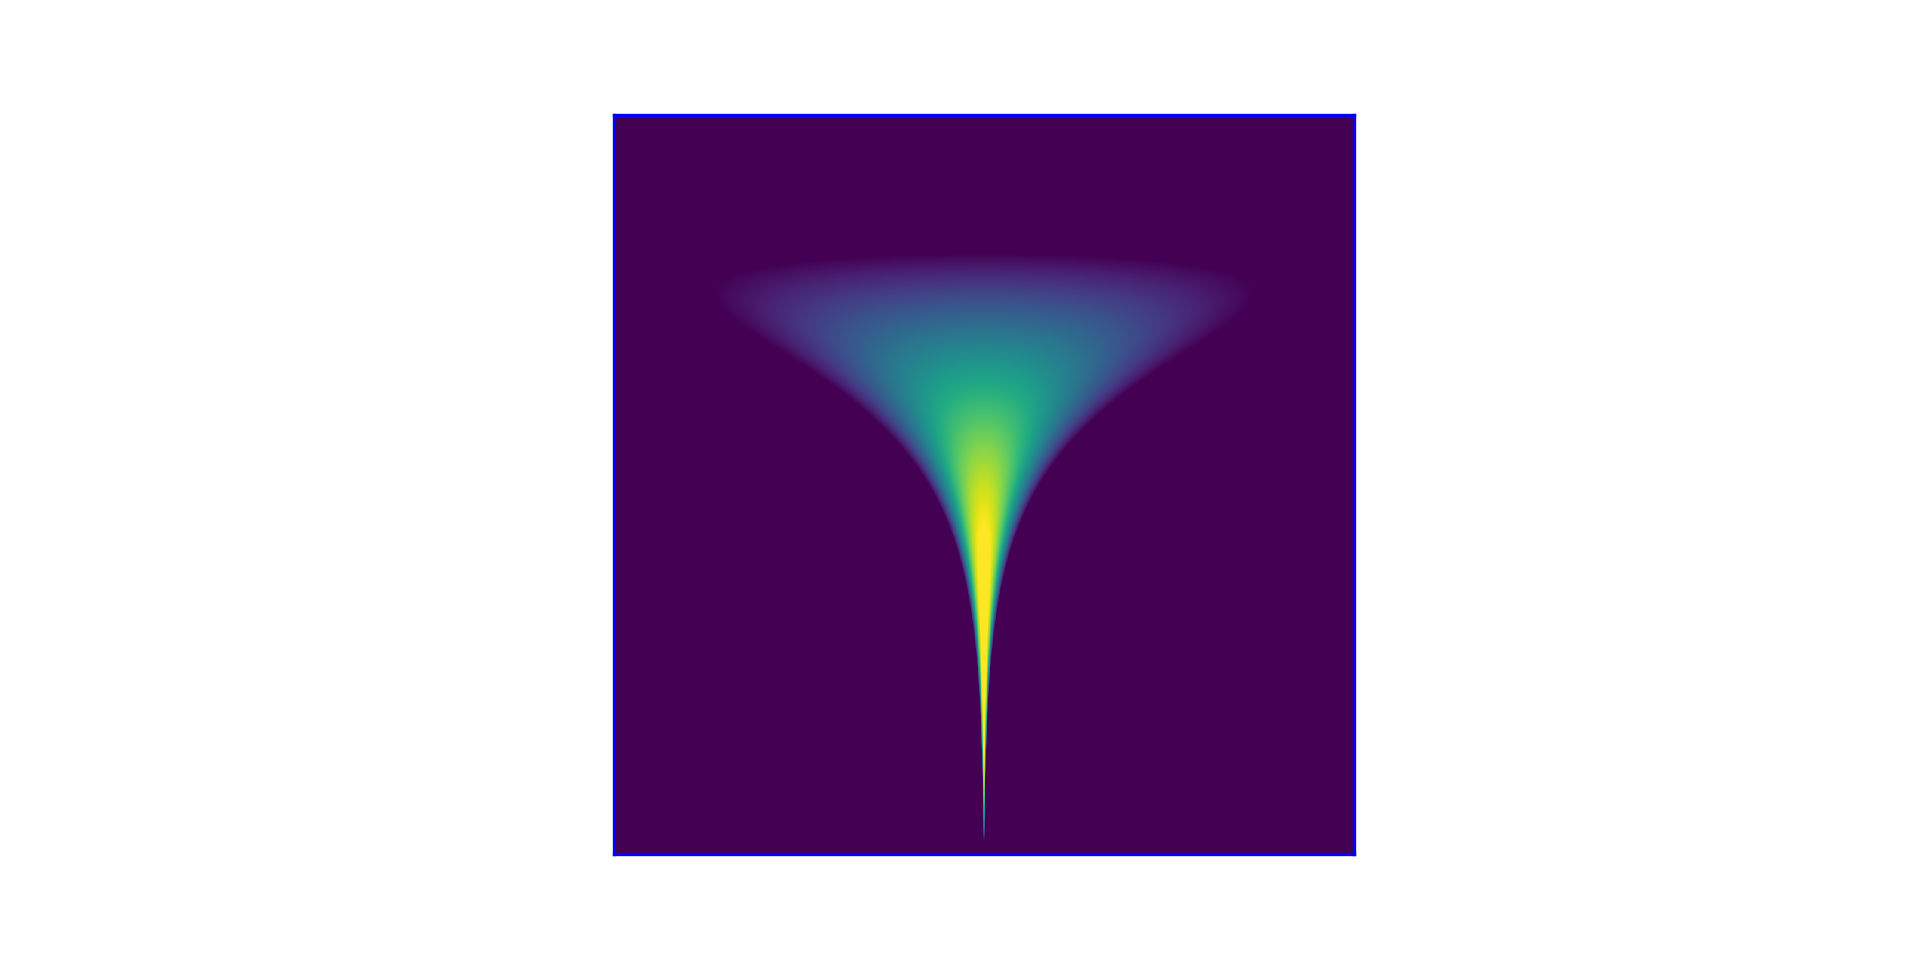
\includegraphics[width=0.65\textwidth]{funnel.png}
\end{frame}

\begin{frame}{Funil de \textcite{nealSliceSampling2003} e Parametrização Não-Centralizada\footnote{\textit{Non-Centered Parametrization} (NCP)}}
  \small
  O funil ocorre quando temos uma variável que a sua variância depende da variância
  de outra em uma escala exponencial. Um exemplo canônico de uma parametrização
  centralizada é:
  $$
  P(y,x) = \text{Normal}(y \mid 0 ,3) \cdot
  \text{Normal}\left(x \mid 0, e^{\left(\frac{y}{2}\right)}\right)
  $$
  Isto ocorre bastante em modelos hierárquicos, na relação dos \textit{prioris} de grupo
  com a(s) \textit{hiperpriori(s)} global(is). Então, reparametrizamos de maneira
  não-centrada alterando a geometria da posterior para facilitar a vida do amostrador
  MCMC:
  $$
  \begin{aligned}
    P(\tilde{y},\tilde{x}) &= \text{Normal}(\tilde{y} \mid 0, 1) \cdot
  \text{Normal}(\tilde{x} \mid 0, 1) \\
    y &= \tilde{y} \cdot 3 + 0 \\
    x &= \tilde{x} \cdot  e^{\left(\frac{y}{2}\right)} + 0
  \end{aligned}
  $$
\end{frame}

\begin{frame}{\href{https://mc-stan.org}{\texttt{Stan}} e NUTS}
  \href{https://mc-stan.org}{\texttt{Stan}} foi o primeiro amostrador MCMC a
  implementar NUTS. Além disso tem uma rotina otimizada automática de ajuste de $L$
  e $\epsilon$ durante a fase de \textit{warmup}. Possui os seguintes valores como
  hiperparâmetros padrões do NUTS\footnote{para mais informações sobre como
  modificar esses hiperparâmetros consulte a \href{
    https://mc-stan.org/docs/reference-manual/hmc-algorithm-parameters.html}{
    Seção 15.2 do \textit{Stan Reference Manual}}}:
  \begin{vfilleditems}
    \item \textbf{Taxa-alvo de aceitação de propostas Metropolis}: \lstinline!adapt_delta = 0.8!
    \item \textbf{Profundidade máxima de árvore} (em potências de 2): \lstinline!max_treedepth = 10! (quer dizer $2^{10} = 1024$)
  \end{vfilleditems}
\end{frame}

\subsection{Convergência de Correntes Markov}
\begin{frame}{Convergência de Correntes Markov}
  MCMC tem uma propriedade interessante que é garantido que \textbf{assintoticamente ele convergirá
  à distribuição-alvo}.
  \vfill
  Ou seja, se tivermos todo o tempo do mundo, é garantido que, irrelevante da geometria
  da distribuição-alvo (posterior), \textbf{MCMC irá lhe dar a resposta correta}.
  \vfill
  Porém não temos todo o tempo do mundo. Diferentes algoritmos MCMC, como HMC e NUTS,
  podem reduzir o tempo de amostragem (e \textit{warmup}) necessários para convergência.
\end{frame}

\subsubsection{Métricas de Convergência}
\begin{frame}{Métricas de Convergência}
  Temos algumas maneiras de mensurar se as correntes Markov convergiram à distribuição-alvo,
  \textit{i.e.} são "confiáveis":
  \begin{vfilleditems}
    \item Número de Amostras Efetivas (\textit{Effective Sample Size} -- ESS):
    uma aproximação do "número de amostras independentes"~geradas por uma corrente Markov.
    \item $\widehat{R}$ (\textit{Rhat}):
    escala de \textbf{R}edução potencial, uma métrica de mensuração que as correntes
    Markov se "misturaram", e, potencialmente, convergiram
  \end{vfilleditems}
\end{frame}

\begin{frame}{Métricas de Convergência - \textit{Effective Sample Size} \parencite{gelman2013bayesian}}
  $$\widehat{n}_{\text{eff}} = \frac{mn}{1 + \sum_{t=1}^T \widehat{\rho}_t}$$
  Onde:
  \begin{vfilleditems}
    \item $m$: número de correntes Markov
    \item $n$: amostras totais por corrente Markov (descontando \textit{warmup})
    \item $\widehat{\rho}_t$: uma estimativa de autocorrelação
  \end{vfilleditems}
\end{frame}

\begin{frame}{Métricas de Convergência - \textit{Rhat} \parencite{gelman2013bayesian}}
  $$\widehat{R} = \sqrt{\frac{\widehat{\text{var}}^+(\psi \mid y)}{W}}$$
  onde a $\widehat{\text{var}}^+(\psi \mid y)$ é a variância das amostras das
  correntes Markov para um determinado parâmetro $\psi$ sob uma média ponderada
  das variâncias intra-correntes (\textit{within-chain}) $W$ e inter-correntes
  (\textit{between-chain}) $B$
  $$\widehat{\text{var}}^+(\psi \mid y) = \frac{n-1}{n} W + \frac{1}{n} B$$
  Intuitivamente, seu valor é $1.0$ se as correntes estiverem totalmente convergentes.
  Como uma heurística, se $\widehat{R}$ for maior que $1.1$, você deve se preocupar pois
  provavelmente as correntes não tenham convergido adequadamente.
\end{frame}

\subsubsection{Visualizações de Convergência}
\begin{frame}{\textit{Traceplot} -- Correntes Markov Convergentes}
  \begin{figure}
    \centering
    \resizebox{.4\linewidth}{!}{% Created by tikzDevice version 0.12.3.1 on 2021-05-31 11:59:55
% !TEX encoding = UTF-8 Unicode
\begin{tikzpicture}[x=1pt,y=1pt]
\definecolor{fillColor}{RGB}{255,255,255}
\path[use as bounding box,fill=fillColor,fill opacity=0.00] (0,0) rectangle (505.89,505.89);
\begin{scope}
\path[clip] (  0.00,  0.00) rectangle (505.89,505.89);
\definecolor{drawColor}{RGB}{0,0,0}
\definecolor{fillColor}{RGB}{0,0,0}

\path[draw=drawColor,line width= 0.6pt,line join=round,line cap=round,fill=fillColor] (  0.00,  0.00) rectangle (505.89,505.89);
\end{scope}
\begin{scope}
\path[clip] ( 22.18, 18.22) rectangle (449.67,500.39);
\definecolor{fillColor}{RGB}{0,0,0}

\path[fill=fillColor] ( 22.18, 18.22) rectangle (449.67,500.39);
\definecolor{drawColor}{gray}{0.13}

\path[draw=drawColor,line width= 0.1pt,line join=round] ( 22.18, 76.16) --
	(449.67, 76.16);

\path[draw=drawColor,line width= 0.1pt,line join=round] ( 22.18,171.51) --
	(449.67,171.51);

\path[draw=drawColor,line width= 0.1pt,line join=round] ( 22.18,266.86) --
	(449.67,266.86);

\path[draw=drawColor,line width= 0.1pt,line join=round] ( 22.18,362.20) --
	(449.67,362.20);

\path[draw=drawColor,line width= 0.1pt,line join=round] ( 22.18,457.55) --
	(449.67,457.55);

\path[draw=drawColor,line width= 0.1pt,line join=round] ( 84.36, 18.22) --
	( 84.36,500.39);

\path[draw=drawColor,line width= 0.1pt,line join=round] (170.72, 18.22) --
	(170.72,500.39);

\path[draw=drawColor,line width= 0.1pt,line join=round] (257.09, 18.22) --
	(257.09,500.39);

\path[draw=drawColor,line width= 0.1pt,line join=round] (343.45, 18.22) --
	(343.45,500.39);

\path[draw=drawColor,line width= 0.1pt,line join=round] (429.81, 18.22) --
	(429.81,500.39);

\path[draw=drawColor,line width= 0.3pt,line join=round] ( 22.18, 28.49) --
	(449.67, 28.49);

\path[draw=drawColor,line width= 0.3pt,line join=round] ( 22.18,123.84) --
	(449.67,123.84);

\path[draw=drawColor,line width= 0.3pt,line join=round] ( 22.18,219.18) --
	(449.67,219.18);

\path[draw=drawColor,line width= 0.3pt,line join=round] ( 22.18,314.53) --
	(449.67,314.53);

\path[draw=drawColor,line width= 0.3pt,line join=round] ( 22.18,409.88) --
	(449.67,409.88);

\path[draw=drawColor,line width= 0.3pt,line join=round] ( 41.18, 18.22) --
	( 41.18,500.39);

\path[draw=drawColor,line width= 0.3pt,line join=round] (127.54, 18.22) --
	(127.54,500.39);

\path[draw=drawColor,line width= 0.3pt,line join=round] (213.91, 18.22) --
	(213.91,500.39);

\path[draw=drawColor,line width= 0.3pt,line join=round] (300.27, 18.22) --
	(300.27,500.39);

\path[draw=drawColor,line width= 0.3pt,line join=round] (386.63, 18.22) --
	(386.63,500.39);
\definecolor{drawColor}{RGB}{1,31,75}

\path[draw=drawColor,line width= 0.4pt,line join=round] ( 41.61,222.92) --
	( 42.04,204.96) --
	( 42.48,206.25) --
	( 42.91,165.69) --
	( 43.34,165.69) --
	( 43.77,163.58) --
	( 44.20,221.08) --
	( 44.63,210.00) --
	( 45.07,275.91) --
	( 45.50,136.32) --
	( 45.93,248.08) --
	( 46.36,228.21) --
	( 46.79,218.61) --
	( 47.23,245.67) --
	( 47.66,213.48) --
	( 48.09,255.03) --
	( 48.52,158.23) --
	( 48.95,299.50) --
	( 49.38,341.55) --
	( 49.82,283.34) --
	( 50.25,283.34) --
	( 50.68,118.63) --
	( 51.11,204.07) --
	( 51.54,217.46) --
	( 51.98,247.07) --
	( 52.41,165.21) --
	( 52.84,165.58) --
	( 53.27,244.06) --
	( 53.70,170.69) --
	( 54.13,217.63) --
	( 54.57,225.28) --
	( 55.00,221.31) --
	( 55.43,189.70) --
	( 55.86,170.14) --
	( 56.29,251.82) --
	( 56.73,241.96) --
	( 57.16,197.19) --
	( 57.59,290.64) --
	( 58.02,228.73) --
	( 58.45,298.48) --
	( 58.88,202.02) --
	( 59.32,187.21) --
	( 59.75,167.25) --
	( 60.18,185.49) --
	( 60.61,185.49) --
	( 61.04,209.39) --
	( 61.48,249.73) --
	( 61.91,229.47) --
	( 62.34,229.47) --
	( 62.77,207.24) --
	( 63.20,145.54) --
	( 63.63,251.30) --
	( 64.07,246.69) --
	( 64.50,246.69) --
	( 64.93,246.69) --
	( 65.36,226.98) --
	( 65.79,158.71) --
	( 66.23,226.74) --
	( 66.66,228.86) --
	( 67.09,219.07) --
	( 67.52,271.03) --
	( 67.95,236.38) --
	( 68.38,247.12) --
	( 68.82,207.82) --
	( 69.25,176.18) --
	( 69.68,267.48) --
	( 70.11,179.57) --
	( 70.54,295.11) --
	( 70.98,205.16) --
	( 71.41,231.62) --
	( 71.84,231.62) --
	( 72.27,240.95) --
	( 72.70,240.95) --
	( 73.13,196.06) --
	( 73.57,190.89) --
	( 74.00,190.89) --
	( 74.43,227.82) --
	( 74.86,203.44) --
	( 75.29,203.44) --
	( 75.73,259.20) --
	( 76.16,134.68) --
	( 76.59,265.00) --
	( 77.02,145.18) --
	( 77.45,265.84) --
	( 77.88,168.13) --
	( 78.32,310.48) --
	( 78.75,108.72) --
	( 79.18,298.87) --
	( 79.61,348.38) --
	( 80.04,302.02) --
	( 80.48,182.41) --
	( 80.91,299.84) --
	( 81.34,294.94) --
	( 81.77,200.94) --
	( 82.20,261.79) --
	( 82.63,282.66) --
	( 83.07,258.84) --
	( 83.50,174.13) --
	( 83.93,123.91) --
	( 84.36,123.91) --
	( 84.79,177.59) --
	( 85.23,267.42) --
	( 85.66,225.41) --
	( 86.09,225.87) --
	( 86.52,155.73) --
	( 86.95,223.15) --
	( 87.38,292.38) --
	( 87.82,165.90) --
	( 88.25,293.99) --
	( 88.68,111.82) --
	( 89.11,308.27) --
	( 89.54,192.52) --
	( 89.98,216.75) --
	( 90.41,233.78) --
	( 90.84,336.24) --
	( 91.27,257.34) --
	( 91.70,223.61) --
	( 92.13,237.18) --
	( 92.57,195.07) --
	( 93.00,189.85) --
	( 93.43,223.60) --
	( 93.86,198.09) --
	( 94.29,199.33) --
	( 94.72,254.04) --
	( 95.16,254.04) --
	( 95.59,109.19) --
	( 96.02,307.88) --
	( 96.45,144.58) --
	( 96.88,176.90) --
	( 97.32,267.32) --
	( 97.75,209.88) --
	( 98.18,230.93) --
	( 98.61,159.53) --
	( 99.04,310.33) --
	( 99.47,164.82) --
	( 99.91,264.89) --
	(100.34,261.06) --
	(100.77,326.53) --
	(101.20,122.36) --
	(101.63,308.11) --
	(102.07,212.60) --
	(102.50,266.07) --
	(102.93,260.38) --
	(103.36,156.96) --
	(103.79,272.85) --
	(104.22,272.85) --
	(104.66,176.68) --
	(105.09,289.38) --
	(105.52,105.81) --
	(105.95,302.47) --
	(106.38,272.05) --
	(106.82,306.64) --
	(107.25,306.64) --
	(107.68,169.46) --
	(108.11,196.34) --
	(108.54,162.32) --
	(108.97,283.98) --
	(109.41,252.06) --
	(109.84,185.97) --
	(110.27,260.11) --
	(110.70,119.57) --
	(111.13,165.42) --
	(111.57,190.26) --
	(112.00,260.97) --
	(112.43,264.92) --
	(112.86,192.31) --
	(113.29,192.31) --
	(113.72,251.86) --
	(114.16,212.46) --
	(114.59,210.38) --
	(115.02,236.67) --
	(115.45,253.40) --
	(115.88,268.63) --
	(116.32,294.83) --
	(116.75, 97.84) --
	(117.18,107.08) --
	(117.61,183.53) --
	(118.04,250.33) --
	(118.47,284.46) --
	(118.91,207.24) --
	(119.34,287.32) --
	(119.77,276.65) --
	(120.20,169.57) --
	(120.63,158.92) --
	(121.07,188.43) --
	(121.50,215.85) --
	(121.93,266.11) --
	(122.36,155.30) --
	(122.79,284.70) --
	(123.22,115.02) --
	(123.66,311.31) --
	(124.09,131.66) --
	(124.52,146.35) --
	(124.95,288.28) --
	(125.38,291.99) --
	(125.82,308.56) --
	(126.25,210.54) --
	(126.68,182.48) --
	(127.11,230.44) --
	(127.54,206.43) --
	(127.97,209.22) --
	(128.41,151.90) --
	(128.84,270.42) --
	(129.27,172.92) --
	(129.70,269.16) --
	(130.13,161.18) --
	(130.57,219.84) --
	(131.00,267.06) --
	(131.43,267.06) --
	(131.86,267.06) --
	(132.29,394.56) --
	(132.72,162.09) --
	(133.16,320.31) --
	(133.59,322.13) --
	(134.02,332.88) --
	(134.45,127.98) --
	(134.88,130.69) --
	(135.32,272.58) --
	(135.75,338.32) --
	(136.18,259.09) --
	(136.61,212.76) --
	(137.04,154.32) --
	(137.47,147.11) --
	(137.91,147.11) --
	(138.34,316.23) --
	(138.77,316.23) --
	(139.20,174.68) --
	(139.63,275.28) --
	(140.07,245.70) --
	(140.50,225.62) --
	(140.93,225.62) --
	(141.36,160.81) --
	(141.79,211.09) --
	(142.22,201.63) --
	(142.66,201.63) --
	(143.09,203.07) --
	(143.52,160.90) --
	(143.95,158.15) --
	(144.38,240.01) --
	(144.82,208.37) --
	(145.25,323.11) --
	(145.68,218.63) --
	(146.11,228.25) --
	(146.54,235.61) --
	(146.97,195.45) --
	(147.41,241.57) --
	(147.84,238.44) --
	(148.27,194.05) --
	(148.70,238.79) --
	(149.13,304.87) --
	(149.57,304.87) --
	(150.00,154.25) --
	(150.43,295.19) --
	(150.86,214.66) --
	(151.29,185.17) --
	(151.72,247.93) --
	(152.16,204.36) --
	(152.59,349.52) --
	(153.02,131.11) --
	(153.45,247.59) --
	(153.88,298.77) --
	(154.32,192.19) --
	(154.75,232.17) --
	(155.18,179.93) --
	(155.61,232.53) --
	(156.04,244.37) --
	(156.47,233.66) --
	(156.91,260.53) --
	(157.34,176.14) --
	(157.77,192.72) --
	(158.20,234.69) --
	(158.63,216.74) --
	(159.07,216.74) --
	(159.50,236.61) --
	(159.93,236.61) --
	(160.36,236.61) --
	(160.79,204.45) --
	(161.22,235.53) --
	(161.66,235.53) --
	(162.09,243.95) --
	(162.52,152.44) --
	(162.95,199.80) --
	(163.38,220.79) --
	(163.81,242.29) --
	(164.25,277.88) --
	(164.68,300.31) --
	(165.11,211.07) --
	(165.54,268.21) --
	(165.97,268.21) --
	(166.41,268.21) --
	(166.84,165.59) --
	(167.27,282.95) --
	(167.70,184.84) --
	(168.13,202.35) --
	(168.56,202.35) --
	(169.00,202.35) --
	(169.43,204.21) --
	(169.86,212.66) --
	(170.29,203.46) --
	(170.72,162.25) --
	(171.16,269.40) --
	(171.59,154.24) --
	(172.02,271.32) --
	(172.45,132.51) --
	(172.88,132.51) --
	(173.31,334.59) --
	(173.75,102.61) --
	(174.18,101.20) --
	(174.61,149.64) --
	(175.04,250.80) --
	(175.47,245.24) --
	(175.91,173.38) --
	(176.34,135.21) --
	(176.77,135.21) --
	(177.20,159.79) --
	(177.63,261.28) --
	(178.06,259.53) --
	(178.50,183.64) --
	(178.93,255.55) --
	(179.36,255.55) --
	(179.79,287.98) --
	(180.22,152.39) --
	(180.66,224.90) --
	(181.09,197.18) --
	(181.52,262.95) --
	(181.95,229.53) --
	(182.38,254.11) --
	(182.81,254.11) --
	(183.25,235.41) --
	(183.68,224.39) --
	(184.11,232.92) --
	(184.54, 74.82) --
	(184.97,347.62) --
	(185.41,168.41) --
	(185.84,166.59) --
	(186.27,236.73) --
	(186.70,236.73) --
	(187.13,214.30) --
	(187.56,285.52) --
	(188.00,173.92) --
	(188.43,235.52) --
	(188.86,146.72) --
	(189.29,302.12) --
	(189.72,345.93) --
	(190.16,113.05) --
	(190.59,283.45) --
	(191.02,175.61) --
	(191.45,233.57) --
	(191.88,263.54) --
	(192.31,273.09) --
	(192.75,123.35) --
	(193.18,277.14) --
	(193.61,152.00) --
	(194.04,261.74) --
	(194.47,238.10) --
	(194.91,178.76) --
	(195.34,283.52) --
	(195.77,230.76) --
	(196.20,325.23) --
	(196.63,325.23) --
	(197.06,298.16) --
	(197.50,275.75) --
	(197.93,176.93) --
	(198.36,203.33) --
	(198.79,203.33) --
	(199.22,130.22) --
	(199.66,257.99) --
	(200.09,257.99) --
	(200.52,190.68) --
	(200.95,215.00) --
	(201.38,255.58) --
	(201.81,226.40) --
	(202.25,209.04) --
	(202.68,166.48) --
	(203.11,226.76) --
	(203.54,234.61) --
	(203.97,170.36) --
	(204.41,271.08) --
	(204.84,271.08) --
	(205.27,166.11) --
	(205.70,154.54) --
	(206.13,228.03) --
	(206.56,228.03) --
	(207.00,328.11) --
	(207.43,267.36) --
	(207.86,248.84) --
	(208.29,159.32) --
	(208.72,277.74) --
	(209.16,159.95) --
	(209.59,259.92) --
	(210.02,251.69) --
	(210.45,176.92) --
	(210.88, 88.49) --
	(211.31,326.99) --
	(211.75,302.15) --
	(212.18,130.73) --
	(212.61,122.77) --
	(213.04,231.55) --
	(213.47,298.38) --
	(213.91,208.92) --
	(214.34,183.21) --
	(214.77,266.11) --
	(215.20,328.92) --
	(215.63,275.58) --
	(216.06,228.15) --
	(216.50,190.04) --
	(216.93,337.48) --
	(217.36,237.22) --
	(217.79,235.90) --
	(218.22,235.90) --
	(218.66,250.22) --
	(219.09,195.27) --
	(219.52,269.65) --
	(219.95,234.71) --
	(220.38,135.94) --
	(220.81,216.79) --
	(221.25,216.79) --
	(221.68,146.71) --
	(222.11,187.27) --
	(222.54,190.58) --
	(222.97,199.96) --
	(223.41,191.56) --
	(223.84,190.99) --
	(224.27,259.67) --
	(224.70,168.18) --
	(225.13, 96.15) --
	(225.56,302.60) --
	(226.00,267.27) --
	(226.43,127.44) --
	(226.86,319.59) --
	(227.29,298.08) --
	(227.72,124.84) --
	(228.15,315.52) --
	(228.59,215.33) --
	(229.02,200.82) --
	(229.45,163.51) --
	(229.88,163.51) --
	(230.31,169.58) --
	(230.75,221.82) --
	(231.18,182.37) --
	(231.61,255.83) --
	(232.04,201.28) --
	(232.47,190.94) --
	(232.90,127.05) --
	(233.34,164.62) --
	(233.77,204.86) --
	(234.20,272.92) --
	(234.63,213.36) --
	(235.06,234.81) --
	(235.50,195.33) --
	(235.93,241.61) --
	(236.36,241.61) --
	(236.79,199.72) --
	(237.22,230.39) --
	(237.65,137.58) --
	(238.09,210.85) --
	(238.52,213.95) --
	(238.95,229.59) --
	(239.38,229.59) --
	(239.81,216.47) --
	(240.25,213.41) --
	(240.68,201.11) --
	(241.11,201.11) --
	(241.54,231.57) --
	(241.97,251.95) --
	(242.40,222.13) --
	(242.84,327.31) --
	(243.27,332.60) --
	(243.70,231.15) --
	(244.13,214.30) --
	(244.56,308.26) --
	(245.00,311.94) --
	(245.43,150.45) --
	(245.86,173.45) --
	(246.29,124.31) --
	(246.72,357.41) --
	(247.15,285.56) --
	(247.59,268.10) --
	(248.02,207.97) --
	(248.45,246.58) --
	(248.88,266.35) --
	(249.31,295.27) --
	(249.75,172.91) --
	(250.18,299.37) --
	(250.61,149.03) --
	(251.04,274.35) --
	(251.47,208.32) --
	(251.90,228.02) --
	(252.34,184.53) --
	(252.77,284.84) --
	(253.20,136.83) --
	(253.63,191.44) --
	(254.06,171.04) --
	(254.50,245.65) --
	(254.93,206.81) --
	(255.36,125.98) --
	(255.79,326.46) --
	(256.22,127.62) --
	(256.65,179.01) --
	(257.09,141.07) --
	(257.52,156.26) --
	(257.95,299.85) --
	(258.38,155.33) --
	(258.81,190.77) --
	(259.25,110.71) --
	(259.68,231.06) --
	(260.11,202.37) --
	(260.54,227.10) --
	(260.97,230.19) --
	(261.40,190.56) --
	(261.84,249.98) --
	(262.27,208.94) --
	(262.70,261.17) --
	(263.13,202.73) --
	(263.56,294.85) --
	(264.00,191.59) --
	(264.43,251.84) --
	(264.86,251.84) --
	(265.29,179.27) --
	(265.72,262.38) --
	(266.15,262.38) --
	(266.59,255.59) --
	(267.02,249.27) --
	(267.45,222.41) --
	(267.88,291.33) --
	(268.31,292.64) --
	(268.75,164.48) --
	(269.18,253.44) --
	(269.61,165.61) --
	(270.04,309.71) --
	(270.47,208.44) --
	(270.90,245.62) --
	(271.34,163.88) --
	(271.77,134.74) --
	(272.20,291.18) --
	(272.63,291.18) --
	(273.06,106.19) --
	(273.50,186.97) --
	(273.93,186.97) --
	(274.36,278.80) --
	(274.79,231.40) --
	(275.22,231.40) --
	(275.65,232.42) --
	(276.09,240.48) --
	(276.52,241.07) --
	(276.95,217.04) --
	(277.38,221.04) --
	(277.81,221.04) --
	(278.25,201.56) --
	(278.68,201.56) --
	(279.11,148.95) --
	(279.54,277.11) --
	(279.97,150.00) --
	(280.40,303.33) --
	(280.84,129.74) --
	(281.27,349.46) --
	(281.70,147.02) --
	(282.13,345.55) --
	(282.56,176.98) --
	(283.00,188.20) --
	(283.43,251.89) --
	(283.86,251.89) --
	(284.29,328.82) --
	(284.72, 91.94) --
	(285.15,166.38) --
	(285.59,253.28) --
	(286.02,215.18) --
	(286.45,181.22) --
	(286.88,173.32) --
	(287.31,248.83) --
	(287.75,197.16) --
	(288.18,197.16) --
	(288.61,196.87) --
	(289.04,254.67) --
	(289.47,206.59) --
	(289.90,202.92) --
	(290.34,272.60) --
	(290.77,272.60) --
	(291.20,249.27) --
	(291.63,226.12) --
	(292.06,165.31) --
	(292.49,288.85) --
	(292.93,129.91) --
	(293.36,130.14) --
	(293.79,349.38) --
	(294.22,192.39) --
	(294.65,309.69) --
	(295.09,165.65) --
	(295.52,228.50) --
	(295.95,223.66) --
	(296.38,169.82) --
	(296.81,226.73) --
	(297.24,307.66) --
	(297.68,217.37) --
	(298.11,265.96) --
	(298.54,206.11) --
	(298.97,151.02) --
	(299.40,109.85) --
	(299.84,123.71) --
	(300.27,303.13) --
	(300.70,128.47) --
	(301.13,150.23) --
	(301.56,176.60) --
	(301.99,193.33) --
	(302.43,231.98) --
	(302.86,245.01) --
	(303.29,216.83) --
	(303.72,222.26) --
	(304.15,222.26) --
	(304.59,198.91) --
	(305.02,153.94) --
	(305.45,339.80) --
	(305.88,127.20) --
	(306.31,330.91) --
	(306.74,281.91) --
	(307.18,182.56) --
	(307.61,184.79) --
	(308.04,253.58) --
	(308.47,392.28) --
	(308.90,331.12) --
	(309.34,317.02) --
	(309.77,148.46) --
	(310.20,147.44) --
	(310.63,269.75) --
	(311.06,135.06) --
	(311.49, 90.91) --
	(311.93,156.05) --
	(312.36,197.55) --
	(312.79,221.32) --
	(313.22,221.32) --
	(313.65,221.32) --
	(314.09,195.69) --
	(314.52,195.69) --
	(314.95,195.69) --
	(315.38,242.20) --
	(315.81,229.43) --
	(316.24,255.22) --
	(316.68,181.19) --
	(317.11,167.40) --
	(317.54,134.34) --
	(317.97,189.22) --
	(318.40,158.51) --
	(318.84,285.93) --
	(319.27,285.93) --
	(319.70,258.19) --
	(320.13,166.52) --
	(320.56,166.52) --
	(320.99,180.45) --
	(321.43,143.65) --
	(321.86,325.23) --
	(322.29,133.99) --
	(322.72,259.48) --
	(323.15,256.00) --
	(323.59,225.65) --
	(324.02,236.00) --
	(324.45,190.69) --
	(324.88,183.95) --
	(325.31,183.95) --
	(325.74,301.59) --
	(326.18,192.65) --
	(326.61,254.26) --
	(327.04,193.38) --
	(327.47,193.38) --
	(327.90,193.38) --
	(328.34,298.42) --
	(328.77,175.38) --
	(329.20,229.10) --
	(329.63,166.47) --
	(330.06,289.73) --
	(330.49,310.16) --
	(330.93,180.70) --
	(331.36,271.44) --
	(331.79,271.44) --
	(332.22,271.44) --
	(332.65,176.35) --
	(333.09,199.79) --
	(333.52,190.79) --
	(333.95,160.47) --
	(334.38,178.70) --
	(334.81,235.40) --
	(335.24,235.40) --
	(335.68,259.46) --
	(336.11,194.78) --
	(336.54, 82.93) --
	(336.97,169.26) --
	(337.40,169.26) --
	(337.84,285.08) --
	(338.27,373.12) --
	(338.70, 74.48) --
	(339.13,224.20) --
	(339.56,205.27) --
	(339.99,235.04) --
	(340.43,183.83) --
	(340.86,269.12) --
	(341.29,204.64) --
	(341.72,204.64) --
	(342.15,207.61) --
	(342.59,207.61) --
	(343.02,233.97) --
	(343.45,211.41) --
	(343.88,178.97) --
	(344.31,229.10) --
	(344.74,209.40) --
	(345.18,230.53) --
	(345.61,177.00) --
	(346.04,177.00) --
	(346.47,208.45) --
	(346.90,232.31) --
	(347.34,232.31) --
	(347.77,218.24) --
	(348.20,178.46) --
	(348.63,210.78) --
	(349.06,223.38) --
	(349.49,148.16) --
	(349.93,187.60) --
	(350.36,304.81) --
	(350.79,202.83) --
	(351.22,178.83) --
	(351.65,282.48) --
	(352.09,259.02) --
	(352.52,227.95) --
	(352.95,145.31) --
	(353.38,182.12) --
	(353.81,237.71) --
	(354.24,211.53) --
	(354.68,225.72) --
	(355.11,176.48) --
	(355.54,257.87) --
	(355.97,301.04) --
	(356.40,171.04) --
	(356.84,157.68) --
	(357.27,326.41) --
	(357.70,165.22) --
	(358.13,297.57) --
	(358.56,126.57) --
	(358.99,171.48) --
	(359.43,113.92) --
	(359.86,185.06) --
	(360.29,195.50) --
	(360.72,296.52) --
	(361.15,253.24) --
	(361.58,247.84) --
	(362.02,247.84) --
	(362.45,247.84) --
	(362.88,254.19) --
	(363.31,268.92) --
	(363.74,163.51) --
	(364.18,269.30) --
	(364.61,278.35) --
	(365.04,108.89) --
	(365.47,271.72) --
	(365.90,187.49) --
	(366.33,253.87) --
	(366.77,259.66) --
	(367.20,309.19) --
	(367.63,221.37) --
	(368.06,215.77) --
	(368.49,114.75) --
	(368.93,314.41) --
	(369.36,337.09) --
	(369.79,256.52) --
	(370.22,182.67) --
	(370.65,267.88) --
	(371.08,186.19) --
	(371.52,222.47) --
	(371.95,187.22) --
	(372.38,256.10) --
	(372.81,253.19) --
	(373.24,218.23) --
	(373.68,273.10) --
	(374.11,237.77) --
	(374.54,237.77) --
	(374.97,201.22) --
	(375.40,228.29) --
	(375.83,243.17) --
	(376.27,257.22) --
	(376.70,306.58) --
	(377.13,127.08) --
	(377.56,277.21) --
	(377.99,186.99) --
	(378.43,208.62) --
	(378.86,193.28) --
	(379.29,290.02) --
	(379.72,193.50) --
	(380.15,187.27) --
	(380.58,187.27) --
	(381.02,342.22) --
	(381.45,136.69) --
	(381.88,264.38) --
	(382.31,126.53) --
	(382.74, 87.61) --
	(383.18,183.91) --
	(383.61,208.55) --
	(384.04,208.55) --
	(384.47,287.98) --
	(384.90,144.45) --
	(385.33,171.96) --
	(385.77,161.68) --
	(386.20,275.67) --
	(386.63,163.13) --
	(387.06,107.84) --
	(387.49,211.34) --
	(387.93,211.34) --
	(388.36,211.34) --
	(388.79,355.75) --
	(389.22, 74.72) --
	(389.65,337.76) --
	(390.08,319.49) --
	(390.52,126.67) --
	(390.95,265.76) --
	(391.38,187.32) --
	(391.81,274.47) --
	(392.24,145.70) --
	(392.68,145.70) --
	(393.11,208.18) --
	(393.54,315.03) --
	(393.97,298.03) --
	(394.40,187.64) --
	(394.83,296.56) --
	(395.27,329.20) --
	(395.70,222.09) --
	(396.13,261.22) --
	(396.56,232.11) --
	(396.99,227.67) --
	(397.43,203.40) --
	(397.86,232.61) --
	(398.29,242.33) --
	(398.72,173.39) --
	(399.15,256.89) --
	(399.58,164.24) --
	(400.02,240.22) --
	(400.45,290.81) --
	(400.88,290.81) --
	(401.31,139.65) --
	(401.74,234.65) --
	(402.18,193.07) --
	(402.61,166.74) --
	(403.04,207.93) --
	(403.47,137.47) --
	(403.90,264.66) --
	(404.33,264.66) --
	(404.77,191.88) --
	(405.20,250.53) --
	(405.63,202.78) --
	(406.06,292.29) --
	(406.49,340.40) --
	(406.93,314.23) --
	(407.36,325.70) --
	(407.79,146.79) --
	(408.22,293.08) --
	(408.65,162.91) --
	(409.08,341.27) --
	(409.52,281.63) --
	(409.95,253.04) --
	(410.38,193.32) --
	(410.81,252.47) --
	(411.24,225.40) --
	(411.68,169.03) --
	(412.11,169.03) --
	(412.54,258.03) --
	(412.97,206.43) --
	(413.40,257.37) --
	(413.83,114.40) --
	(414.27,170.75) --
	(414.70,278.05) --
	(415.13,233.64) --
	(415.56,233.64) --
	(415.99,233.64) --
	(416.43,213.81) --
	(416.86,206.07) --
	(417.29,270.33) --
	(417.72,216.86) --
	(418.15,216.86) --
	(418.58,263.43) --
	(419.02,182.74) --
	(419.45,188.33) --
	(419.88,206.74) --
	(420.31,191.95) --
	(420.74,163.22) --
	(421.18,331.74) --
	(421.61,247.31) --
	(422.04,353.83) --
	(422.47,267.37) --
	(422.90,107.43) --
	(423.33, 87.23) --
	(423.77,140.28) --
	(424.20,244.59) --
	(424.63,174.86) --
	(425.06,314.97) --
	(425.49,141.40) --
	(425.92,297.38) --
	(426.36,316.27) --
	(426.79,125.15) --
	(427.22,229.29) --
	(427.65,231.32) --
	(428.08,217.68) --
	(428.52,127.34) --
	(428.95,218.00) --
	(429.38,276.85) --
	(429.81,181.89) --
	(430.24,185.78);
\definecolor{drawColor}{RGB}{3,57,108}

\path[draw=drawColor,line width= 0.4pt,line join=round] ( 41.61,175.38) --
	( 42.04,171.48) --
	( 42.48,247.21) --
	( 42.91,192.59) --
	( 43.34,193.15) --
	( 43.77,121.36) --
	( 44.20,320.10) --
	( 44.63,102.00) --
	( 45.07,364.80) --
	( 45.50,237.36) --
	( 45.93,119.36) --
	( 46.36,317.41) --
	( 46.79,297.47) --
	( 47.23,297.68) --
	( 47.66, 61.64) --
	( 48.09,257.57) --
	( 48.52,298.70) --
	( 48.95,298.70) --
	( 49.38,253.32) --
	( 49.82,156.34) --
	( 50.25,247.08) --
	( 50.68,234.39) --
	( 51.11,184.43) --
	( 51.54,268.42) --
	( 51.98,353.70) --
	( 52.41,241.20) --
	( 52.84,236.59) --
	( 53.27,197.10) --
	( 53.70,227.37) --
	( 54.13,175.44) --
	( 54.57,167.76) --
	( 55.00,271.18) --
	( 55.43,200.83) --
	( 55.86,224.78) --
	( 56.29,196.98) --
	( 56.73,196.98) --
	( 57.16,196.98) --
	( 57.59,253.87) --
	( 58.02,157.84) --
	( 58.45,188.79) --
	( 58.88,274.13) --
	( 59.32,274.90) --
	( 59.75,309.89) --
	( 60.18,217.92) --
	( 60.61,198.51) --
	( 61.04,192.78) --
	( 61.48,235.74) --
	( 61.91,219.66) --
	( 62.34,183.60) --
	( 62.77,195.45) --
	( 63.20,225.11) --
	( 63.63,262.14) --
	( 64.07,262.14) --
	( 64.50,192.23) --
	( 64.93,199.70) --
	( 65.36,213.31) --
	( 65.79,167.85) --
	( 66.23,246.59) --
	( 66.66,183.22) --
	( 67.09,141.90) --
	( 67.52,141.90) --
	( 67.95,189.49) --
	( 68.38,176.47) --
	( 68.82,176.47) --
	( 69.25,242.10) --
	( 69.68,181.50) --
	( 70.11,201.68) --
	( 70.54,234.52) --
	( 70.98,165.51) --
	( 71.41,163.19) --
	( 71.84,163.19) --
	( 72.27,104.62) --
	( 72.70,191.08) --
	( 73.13,255.40) --
	( 73.57,170.82) --
	( 74.00,126.15) --
	( 74.43,166.58) --
	( 74.86,166.10) --
	( 75.29,276.67) --
	( 75.73,153.30) --
	( 76.16,105.96) --
	( 76.59,301.19) --
	( 77.02,228.68) --
	( 77.45,263.32) --
	( 77.88,307.46) --
	( 78.32,240.74) --
	( 78.75,240.74) --
	( 79.18,184.38) --
	( 79.61,241.35) --
	( 80.04,241.35) --
	( 80.48,217.36) --
	( 80.91,260.25) --
	( 81.34,182.14) --
	( 81.77,182.14) --
	( 82.20,253.89) --
	( 82.63,146.92) --
	( 83.07,146.92) --
	( 83.50,146.92) --
	( 83.93,146.92) --
	( 84.36,275.47) --
	( 84.79,237.33) --
	( 85.23,237.33) --
	( 85.66,292.64) --
	( 86.09,169.43) --
	( 86.52,164.37) --
	( 86.95,255.11) --
	( 87.38,220.41) --
	( 87.82,182.76) --
	( 88.25,235.72) --
	( 88.68,235.72) --
	( 89.11,309.51) --
	( 89.54,244.16) --
	( 89.98,280.44) --
	( 90.41,176.82) --
	( 90.84,180.13) --
	( 91.27,129.63) --
	( 91.70,279.21) --
	( 92.13,279.21) --
	( 92.57,170.98) --
	( 93.00,263.18) --
	( 93.43,172.96) --
	( 93.86,236.43) --
	( 94.29,111.40) --
	( 94.72,325.54) --
	( 95.16,175.28) --
	( 95.59,154.04) --
	( 96.02,187.87) --
	( 96.45,250.58) --
	( 96.88,191.10) --
	( 97.32,239.29) --
	( 97.75,190.22) --
	( 98.18,190.22) --
	( 98.61,190.22) --
	( 99.04,271.75) --
	( 99.47,234.77) --
	( 99.91,304.20) --
	(100.34,264.35) --
	(100.77,343.85) --
	(101.20,330.74) --
	(101.63,307.54) --
	(102.07,307.54) --
	(102.50,220.76) --
	(102.93,229.02) --
	(103.36,241.12) --
	(103.79,137.56) --
	(104.22,200.27) --
	(104.66,137.75) --
	(105.09,154.23) --
	(105.52,189.31) --
	(105.95,189.31) --
	(106.38,148.64) --
	(106.82,230.78) --
	(107.25,252.38) --
	(107.68,252.38) --
	(108.11,189.04) --
	(108.54,203.33) --
	(108.97,226.61) --
	(109.41,226.61) --
	(109.84,205.69) --
	(110.27,187.79) --
	(110.70,187.79) --
	(111.13,233.06) --
	(111.57,233.06) --
	(112.00,217.32) --
	(112.43,240.12) --
	(112.86,273.59) --
	(113.29,230.17) --
	(113.72,230.17) --
	(114.16,230.17) --
	(114.59,156.83) --
	(115.02,182.84) --
	(115.45,368.49) --
	(115.88,294.91) --
	(116.32,145.44) --
	(116.75,147.80) --
	(117.18,200.05) --
	(117.61,200.05) --
	(118.04,275.40) --
	(118.47,175.88) --
	(118.91,283.13) --
	(119.34,157.36) --
	(119.77,156.32) --
	(120.20,156.32) --
	(120.63,274.22) --
	(121.07,194.66) --
	(121.50,194.66) --
	(121.93,221.76) --
	(122.36,258.54) --
	(122.79,230.51) --
	(123.22,190.99) --
	(123.66,190.99) --
	(124.09,219.17) --
	(124.52,230.22) --
	(124.95,262.15) --
	(125.38,330.57) --
	(125.82,258.65) --
	(126.25,240.28) --
	(126.68,229.30) --
	(127.11,257.05) --
	(127.54,151.57) --
	(127.97,223.50) --
	(128.41,246.29) --
	(128.84,246.29) --
	(129.27,211.20) --
	(129.70,237.99) --
	(130.13,188.81) --
	(130.57,202.86) --
	(131.00,338.00) --
	(131.43,231.41) --
	(131.86,276.36) --
	(132.29,258.99) --
	(132.72,231.18) --
	(133.16,183.94) --
	(133.59,213.81) --
	(134.02,213.81) --
	(134.45,237.11) --
	(134.88,190.32) --
	(135.32,226.60) --
	(135.75,244.33) --
	(136.18,288.53) --
	(136.61,289.65) --
	(137.04,159.11) --
	(137.47,271.14) --
	(137.91,233.41) --
	(138.34,233.41) --
	(138.77,256.35) --
	(139.20,192.07) --
	(139.63,192.07) --
	(140.07,192.07) --
	(140.50,199.58) --
	(140.93,257.68) --
	(141.36,113.82) --
	(141.79,178.31) --
	(142.22,225.51) --
	(142.66,207.15) --
	(143.09,217.02) --
	(143.52,240.93) --
	(143.95,212.45) --
	(144.38,243.03) --
	(144.82,185.78) --
	(145.25,171.66) --
	(145.68,280.19) --
	(146.11,156.90) --
	(146.54,156.90) --
	(146.97,273.29) --
	(147.41,209.24) --
	(147.84,238.50) --
	(148.27,205.95) --
	(148.70,247.59) --
	(149.13,262.24) --
	(149.57,220.00) --
	(150.00,220.00) --
	(150.43,311.41) --
	(150.86,161.54) --
	(151.29,161.54) --
	(151.72,246.27) --
	(152.16,209.61) --
	(152.59,172.59) --
	(153.02,237.04) --
	(153.45,217.22) --
	(153.88,200.33) --
	(154.32,230.01) --
	(154.75,245.66) --
	(155.18,167.91) --
	(155.61,309.11) --
	(156.04,154.86) --
	(156.47,304.48) --
	(156.91,221.02) --
	(157.34,224.16) --
	(157.77,161.37) --
	(158.20,116.24) --
	(158.63, 85.53) --
	(159.07,138.07) --
	(159.50,275.47) --
	(159.93,138.18) --
	(160.36,277.92) --
	(160.79,277.92) --
	(161.22,277.92) --
	(161.66,152.09) --
	(162.09,210.58) --
	(162.52,180.75) --
	(162.95,216.82) --
	(163.38,202.25) --
	(163.81,215.96) --
	(164.25,192.44) --
	(164.68,351.53) --
	(165.11,113.02) --
	(165.54,180.01) --
	(165.97,285.11) --
	(166.41,160.52) --
	(166.84,241.56) --
	(167.27,175.23) --
	(167.70,221.59) --
	(168.13,257.79) --
	(168.56,253.69) --
	(169.00,177.59) --
	(169.43,257.31) --
	(169.86,243.31) --
	(170.29,166.86) --
	(170.72,266.30) --
	(171.16,266.30) --
	(171.59,258.26) --
	(172.02,258.26) --
	(172.45,127.95) --
	(172.88,184.67) --
	(173.31,253.45) --
	(173.75,226.88) --
	(174.18,222.88) --
	(174.61,200.21) --
	(175.04,247.78) --
	(175.47,172.73) --
	(175.91,264.41) --
	(176.34,181.05) --
	(176.77,238.97) --
	(177.20,199.71) --
	(177.63,240.67) --
	(178.06,158.85) --
	(178.50,230.67) --
	(178.93,214.38) --
	(179.36,200.48) --
	(179.79,193.83) --
	(180.22,152.91) --
	(180.66,152.91) --
	(181.09,289.14) --
	(181.52,255.50) --
	(181.95,227.70) --
	(182.38,238.39) --
	(182.81,218.41) --
	(183.25,219.79) --
	(183.68,130.04) --
	(184.11,209.75) --
	(184.54,184.75) --
	(184.97,122.48) --
	(185.41,251.74) --
	(185.84,251.74) --
	(186.27,196.19) --
	(186.70,182.00) --
	(187.13,289.96) --
	(187.56,115.60) --
	(188.00,171.25) --
	(188.43,155.46) --
	(188.86,169.42) --
	(189.29,169.42) --
	(189.72,179.28) --
	(190.16,114.57) --
	(190.59,168.55) --
	(191.02,150.46) --
	(191.45,158.75) --
	(191.88,263.92) --
	(192.31,255.02) --
	(192.75,292.14) --
	(193.18,189.65) --
	(193.61,294.46) --
	(194.04,251.14) --
	(194.47,228.13) --
	(194.91,169.64) --
	(195.34,140.11) --
	(195.77, 74.20) --
	(196.20, 74.20) --
	(196.63,340.75) --
	(197.06,289.60) --
	(197.50,289.60) --
	(197.93,270.54) --
	(198.36,173.83) --
	(198.79,287.03) --
	(199.22,276.38) --
	(199.66,179.85) --
	(200.09,179.85) --
	(200.52,312.45) --
	(200.95,318.04) --
	(201.38,308.81) --
	(201.81,308.81) --
	(202.25,240.36) --
	(202.68,189.59) --
	(203.11,241.85) --
	(203.54,268.00) --
	(203.97,242.45) --
	(204.41,204.12) --
	(204.84,188.13) --
	(205.27,190.43) --
	(205.70,262.22) --
	(206.13,171.01) --
	(206.56,171.01) --
	(207.00,272.59) --
	(207.43,190.42) --
	(207.86,190.42) --
	(208.29,139.51) --
	(208.72,209.13) --
	(209.16,209.13) --
	(209.59,209.13) --
	(210.02,249.06) --
	(210.45,228.99) --
	(210.88,213.86) --
	(211.31,129.94) --
	(211.75,232.95) --
	(212.18,249.67) --
	(212.61,237.12) --
	(213.04,186.91) --
	(213.47,234.74) --
	(213.91,145.55) --
	(214.34,145.55) --
	(214.77,265.09) --
	(215.20,158.17) --
	(215.63,213.08) --
	(216.06,298.12) --
	(216.50,219.80) --
	(216.93,214.22) --
	(217.36,245.19) --
	(217.79,160.07) --
	(218.22,150.47) --
	(218.66,216.87) --
	(219.09,234.05) --
	(219.52,304.64) --
	(219.95,114.18) --
	(220.38,212.33) --
	(220.81,287.18) --
	(221.25,162.22) --
	(221.68,275.84) --
	(222.11,331.04) --
	(222.54,322.07) --
	(222.97,116.87) --
	(223.41,189.52) --
	(223.84,268.60) --
	(224.27,174.23) --
	(224.70,242.18) --
	(225.13,161.23) --
	(225.56,138.79) --
	(226.00,181.47) --
	(226.43,231.70) --
	(226.86,171.95) --
	(227.29,200.94) --
	(227.72,244.36) --
	(228.15,244.36) --
	(228.59,204.17) --
	(229.02,196.07) --
	(229.45,231.09) --
	(229.88,264.47) --
	(230.31,333.70) --
	(230.75,250.16) --
	(231.18,224.88) --
	(231.61,156.37) --
	(232.04,239.75) --
	(232.47,165.07) --
	(232.90,148.75) --
	(233.34,266.77) --
	(233.77,160.81) --
	(234.20,177.81) --
	(234.63,254.35) --
	(235.06,326.06) --
	(235.50,208.48) --
	(235.93,218.55) --
	(236.36,218.55) --
	(236.79,218.55) --
	(237.22,214.63) --
	(237.65,241.15) --
	(238.09, 98.34) --
	(238.52,178.24) --
	(238.95,167.59) --
	(239.38,233.94) --
	(239.81,190.89) --
	(240.25,167.74) --
	(240.68,273.00) --
	(241.11,193.74) --
	(241.54,139.14) --
	(241.97,326.30) --
	(242.40,336.21) --
	(242.84,146.23) --
	(243.27,145.16) --
	(243.70,301.55) --
	(244.13,301.55) --
	(244.56,269.53) --
	(245.00,301.62) --
	(245.43,198.54) --
	(245.86,230.63) --
	(246.29,178.54) --
	(246.72,278.72) --
	(247.15,185.18) --
	(247.59,277.94) --
	(248.02,252.96) --
	(248.45,282.39) --
	(248.88,178.03) --
	(249.31,198.89) --
	(249.75,230.32) --
	(250.18,249.45) --
	(250.61,149.17) --
	(251.04,136.47) --
	(251.47,272.64) --
	(251.90,350.71) --
	(252.34,311.13) --
	(252.77,369.19) --
	(253.20,263.85) --
	(253.63,215.67) --
	(254.06,227.59) --
	(254.50,198.87) --
	(254.93,256.60) --
	(255.36,256.60) --
	(255.79,165.14) --
	(256.22,176.82) --
	(256.65,271.31) --
	(257.09,210.19) --
	(257.52,167.24) --
	(257.95,261.87) --
	(258.38,219.91) --
	(258.81,193.51) --
	(259.25,244.43) --
	(259.68,203.69) --
	(260.11,222.45) --
	(260.54,224.56) --
	(260.97,224.56) --
	(261.40,224.56) --
	(261.84,259.28) --
	(262.27,203.02) --
	(262.70,203.02) --
	(263.13,267.36) --
	(263.56,267.36) --
	(264.00,188.10) --
	(264.43,176.92) --
	(264.86,237.50) --
	(265.29,237.50) --
	(265.72,224.53) --
	(266.15,238.56) --
	(266.59,238.49) --
	(267.02,238.49) --
	(267.45,156.37) --
	(267.88,244.69) --
	(268.31,228.89) --
	(268.75,242.59) --
	(269.18,192.43) --
	(269.61,131.09) --
	(270.04,160.16) --
	(270.47,160.16) --
	(270.90,129.65) --
	(271.34,217.03) --
	(271.77,207.26) --
	(272.20,252.43) --
	(272.63,312.91) --
	(273.06,263.26) --
	(273.50,293.83) --
	(273.93,178.14) --
	(274.36,239.03) --
	(274.79,203.10) --
	(275.22,220.94) --
	(275.65,220.94) --
	(276.09,287.32) --
	(276.52,331.67) --
	(276.95, 89.33) --
	(277.38,180.33) --
	(277.81,180.33) --
	(278.25,180.33) --
	(278.68,180.33) --
	(279.11,250.33) --
	(279.54,232.65) --
	(279.97,232.65) --
	(280.40, 77.38) --
	(280.84,158.07) --
	(281.27,241.60) --
	(281.70,209.40) --
	(282.13,209.40) --
	(282.56,180.12) --
	(283.00,127.74) --
	(283.43,286.23) --
	(283.86,218.03) --
	(284.29,195.88) --
	(284.72,233.35) --
	(285.15,233.35) --
	(285.59,309.46) --
	(286.02,335.61) --
	(286.45,325.26) --
	(286.88,145.58) --
	(287.31,212.32) --
	(287.75,229.74) --
	(288.18,208.42) --
	(288.61,166.18) --
	(289.04,266.19) --
	(289.47,187.76) --
	(289.90,217.62) --
	(290.34,168.87) --
	(290.77,206.17) --
	(291.20,189.54) --
	(291.63,247.58) --
	(292.06,182.11) --
	(292.49,290.47) --
	(292.93,270.17) --
	(293.36,175.26) --
	(293.79,321.20) --
	(294.22,205.64) --
	(294.65,205.64) --
	(295.09,177.11) --
	(295.52,296.05) --
	(295.95,136.90) --
	(296.38,216.73) --
	(296.81,290.84) --
	(297.24,227.72) --
	(297.68,255.61) --
	(298.11,199.67) --
	(298.54,199.67) --
	(298.97,261.06) --
	(299.40,316.58) --
	(299.84,209.39) --
	(300.27,180.87) --
	(300.70,180.87) --
	(301.13,180.87) --
	(301.56,180.87) --
	(301.99,239.25) --
	(302.43,181.54) --
	(302.86,239.76) --
	(303.29,122.15) --
	(303.72,179.70) --
	(304.15,179.70) --
	(304.59,167.68) --
	(305.02,289.48) --
	(305.45,289.48) --
	(305.88,245.87) --
	(306.31,295.05) --
	(306.74,266.57) --
	(307.18,218.42) --
	(307.61,204.39) --
	(308.04,236.22) --
	(308.47,288.49) --
	(308.90,140.54) --
	(309.34,281.98) --
	(309.77,164.42) --
	(310.20,150.55) --
	(310.63,172.05) --
	(311.06,185.73) --
	(311.49,245.15) --
	(311.93,203.96) --
	(312.36,189.95) --
	(312.79,189.95) --
	(313.22,166.23) --
	(313.65,140.21) --
	(314.09,318.34) --
	(314.52,241.37) --
	(314.95,170.28) --
	(315.38,274.12) --
	(315.81,150.86) --
	(316.24,280.11) --
	(316.68,243.92) --
	(317.11,243.92) --
	(317.54,243.92) --
	(317.97,262.80) --
	(318.40,181.34) --
	(318.84,280.53) --
	(319.27,162.75) --
	(319.70,245.20) --
	(320.13,245.20) --
	(320.56,292.16) --
	(320.99,209.43) --
	(321.43,234.33) --
	(321.86,212.31) --
	(322.29,177.61) --
	(322.72,109.86) --
	(323.15,301.62) --
	(323.59,122.58) --
	(324.02,317.23) --
	(324.45,254.68) --
	(324.88,237.34) --
	(325.31,236.13) --
	(325.74,223.79) --
	(326.18,271.25) --
	(326.61,214.70) --
	(327.04,226.34) --
	(327.47,224.06) --
	(327.90,118.22) --
	(328.34,130.85) --
	(328.77,206.69) --
	(329.20,208.27) --
	(329.63,187.92) --
	(330.06,230.47) --
	(330.49,186.55) --
	(330.93,258.22) --
	(331.36,258.22) --
	(331.79,237.52) --
	(332.22,281.87) --
	(332.65,281.87) --
	(333.09,252.76) --
	(333.52,219.51) --
	(333.95,219.51) --
	(334.38,219.51) --
	(334.81,161.20) --
	(335.24,264.88) --
	(335.68,227.03) --
	(336.11,205.65) --
	(336.54,244.53) --
	(336.97,205.34) --
	(337.40,273.58) --
	(337.84, 97.83) --
	(338.27,218.79) --
	(338.70,225.22) --
	(339.13,225.22) --
	(339.56,203.20) --
	(339.99,220.69) --
	(340.43,260.89) --
	(340.86,103.23) --
	(341.29,197.90) --
	(341.72,219.03) --
	(342.15,348.22) --
	(342.59,333.21) --
	(343.02,315.81) --
	(343.45,217.41) --
	(343.88,232.22) --
	(344.31,234.46) --
	(344.74,260.51) --
	(345.18,281.41) --
	(345.61,144.40) --
	(346.04,278.17) --
	(346.47,278.17) --
	(346.90,278.17) --
	(347.34,278.17) --
	(347.77,326.24) --
	(348.20,349.60) --
	(348.63,161.23) --
	(349.06,285.07) --
	(349.49,271.31) --
	(349.93,205.15) --
	(350.36,300.44) --
	(350.79,315.57) --
	(351.22,310.62) --
	(351.65,310.62) --
	(352.09,213.93) --
	(352.52,192.60) --
	(352.95, 87.75) --
	(353.38,131.19) --
	(353.81,322.56) --
	(354.24,322.56) --
	(354.68,305.96) --
	(355.11,216.62) --
	(355.54,240.78) --
	(355.97,207.22) --
	(356.40,299.10) --
	(356.84,133.90) --
	(357.27,180.86) --
	(357.70,262.04) --
	(358.13,160.23) --
	(358.56,177.86) --
	(358.99,177.86) --
	(359.43,180.81) --
	(359.86,270.62) --
	(360.29,230.67) --
	(360.72,233.80) --
	(361.15,211.87) --
	(361.58,211.87) --
	(362.02,254.68) --
	(362.45,210.64) --
	(362.88,231.29) --
	(363.31,290.22) --
	(363.74,235.83) --
	(364.18,309.42) --
	(364.61,215.83) --
	(365.04,219.66) --
	(365.47,128.35) --
	(365.90,295.34) --
	(366.33,314.89) --
	(366.77,146.48) --
	(367.20,296.16) --
	(367.63,296.16) --
	(368.06,144.24) --
	(368.49,191.99) --
	(368.93,162.92) --
	(369.36,299.89) --
	(369.79,158.41) --
	(370.22,128.72) --
	(370.65,312.68) --
	(371.08,147.80) --
	(371.52,321.61) --
	(371.95,316.63) --
	(372.38,126.11) --
	(372.81,223.58) --
	(373.24,175.80) --
	(373.68,255.39) --
	(374.11,343.80) --
	(374.54,235.17) --
	(374.97,223.89) --
	(375.40,223.89) --
	(375.83,223.89) --
	(376.27,223.89) --
	(376.70,173.31) --
	(377.13,250.32) --
	(377.56,217.69) --
	(377.99,247.35) --
	(378.43,131.82) --
	(378.86,172.89) --
	(379.29,180.03) --
	(379.72,241.28) --
	(380.15,171.13) --
	(380.58,171.13) --
	(381.02,254.48) --
	(381.45,290.30) --
	(381.88,201.20) --
	(382.31,256.76) --
	(382.74,256.76) --
	(383.18,256.76) --
	(383.61,218.09) --
	(384.04,348.34) --
	(384.47,151.03) --
	(384.90,151.03) --
	(385.33,187.61) --
	(385.77,260.38) --
	(386.20,249.70) --
	(386.63,183.28) --
	(387.06,293.39) --
	(387.49,293.39) --
	(387.93,118.77) --
	(388.36,213.38) --
	(388.79,260.11) --
	(389.22,215.24) --
	(389.65,176.17) --
	(390.08,176.17) --
	(390.52,256.68) --
	(390.95,240.28) --
	(391.38,214.64) --
	(391.81,203.34) --
	(392.24,216.66) --
	(392.68,267.64) --
	(393.11,308.02) --
	(393.54,282.27) --
	(393.97,282.27) --
	(394.40,144.46) --
	(394.83,294.43) --
	(395.27,180.56) --
	(395.70, 97.55) --
	(396.13,287.35) --
	(396.56,125.54) --
	(396.99,220.70) --
	(397.43,220.70) --
	(397.86,220.70) --
	(398.29,220.70) --
	(398.72,207.94) --
	(399.15,213.89) --
	(399.58,233.87) --
	(400.02,238.56) --
	(400.45,313.78) --
	(400.88,128.88) --
	(401.31,248.49) --
	(401.74,201.16) --
	(402.18,228.15) --
	(402.61,117.88) --
	(403.04,320.07) --
	(403.47,320.07) --
	(403.90,150.27) --
	(404.33,311.12) --
	(404.77,254.50) --
	(405.20,301.19) --
	(405.63,186.16) --
	(406.06,166.53) --
	(406.49,193.25) --
	(406.93,240.84) --
	(407.36,300.58) --
	(407.79,300.58) --
	(408.22,130.10) --
	(408.65,270.01) --
	(409.08,280.76) --
	(409.52,177.45) --
	(409.95,152.20) --
	(410.38,169.39) --
	(410.81,253.61) --
	(411.24,297.31) --
	(411.68,316.11) --
	(412.11,316.11) --
	(412.54,264.13) --
	(412.97,195.80) --
	(413.40,251.53) --
	(413.83,207.08) --
	(414.27,186.26) --
	(414.70,186.26) --
	(415.13,186.26) --
	(415.56,244.99) --
	(415.99,177.47) --
	(416.43,229.01) --
	(416.86,226.27) --
	(417.29,199.72) --
	(417.72,132.07) --
	(418.15,198.01) --
	(418.58,211.68) --
	(419.02,237.07) --
	(419.45,237.85) --
	(419.88,264.65) --
	(420.31,181.84) --
	(420.74,172.53) --
	(421.18,226.59) --
	(421.61,162.11) --
	(422.04,111.07) --
	(422.47,274.53) --
	(422.90,139.62) --
	(423.33,141.80) --
	(423.77,143.38) --
	(424.20,262.11) --
	(424.63,160.89) --
	(425.06,161.93) --
	(425.49,216.50) --
	(425.92,183.13) --
	(426.36,291.88) --
	(426.79,291.88) --
	(427.22,186.47) --
	(427.65,254.20) --
	(428.08,254.20) --
	(428.52,284.07) --
	(428.95,319.11) --
	(429.38,110.67) --
	(429.81,170.06) --
	(430.24,185.90);
\definecolor{drawColor}{RGB}{100,151,177}

\path[draw=drawColor,line width= 0.4pt,line join=round] ( 41.61,198.93) --
	( 42.04,237.79) --
	( 42.48,237.79) --
	( 42.91,237.79) --
	( 43.34,161.79) --
	( 43.77,180.59) --
	( 44.20,206.57) --
	( 44.63,224.98) --
	( 45.07,281.89) --
	( 45.50,213.21) --
	( 45.93,213.21) --
	( 46.36,213.21) --
	( 46.79,128.38) --
	( 47.23,102.05) --
	( 47.66,338.22) --
	( 48.09,132.49) --
	( 48.52,313.44) --
	( 48.95,267.62) --
	( 49.38,236.50) --
	( 49.82,238.78) --
	( 50.25,194.38) --
	( 50.68,157.02) --
	( 51.11,288.88) --
	( 51.54,230.67) --
	( 51.98,242.43) --
	( 52.41,243.05) --
	( 52.84,243.05) --
	( 53.27,151.20) --
	( 53.70,167.71) --
	( 54.13,214.19) --
	( 54.57,199.84) --
	( 55.00,199.84) --
	( 55.43,390.53) --
	( 55.86,402.42) --
	( 56.29, 82.11) --
	( 56.73,193.70) --
	( 57.16,190.31) --
	( 57.59,213.94) --
	( 58.02,211.22) --
	( 58.45,205.54) --
	( 58.88,156.62) --
	( 59.32,173.23) --
	( 59.75,133.92) --
	( 60.18,178.25) --
	( 60.61,186.82) --
	( 61.04,132.85) --
	( 61.48, 75.41) --
	( 61.91,142.39) --
	( 62.34,142.39) --
	( 62.77,142.39) --
	( 63.20,142.39) --
	( 63.63,113.34) --
	( 64.07,241.50) --
	( 64.50,236.20) --
	( 64.93,157.74) --
	( 65.36,234.05) --
	( 65.79,266.00) --
	( 66.23,185.91) --
	( 66.66,179.78) --
	( 67.09,232.68) --
	( 67.52,164.66) --
	( 67.95,287.89) --
	( 68.38,169.52) --
	( 68.82,288.26) --
	( 69.25,270.02) --
	( 69.68,226.26) --
	( 70.11,192.00) --
	( 70.54,192.00) --
	( 70.98,216.64) --
	( 71.41,255.25) --
	( 71.84,160.46) --
	( 72.27,240.14) --
	( 72.70,240.14) --
	( 73.13,227.39) --
	( 73.57,198.09) --
	( 74.00,367.59) --
	( 74.43,190.90) --
	( 74.86,168.73) --
	( 75.29, 99.21) --
	( 75.73,230.17) --
	( 76.16,253.11) --
	( 76.59,189.05) --
	( 77.02,280.86) --
	( 77.45,165.76) --
	( 77.88,165.76) --
	( 78.32,296.44) --
	( 78.75,241.93) --
	( 79.18,241.93) --
	( 79.61,241.93) --
	( 80.04,241.93) --
	( 80.48,311.85) --
	( 80.91,257.36) --
	( 81.34,257.36) --
	( 81.77,282.32) --
	( 82.20,229.15) --
	( 82.63,229.15) --
	( 83.07,218.94) --
	( 83.50,234.81) --
	( 83.93,192.09) --
	( 84.36,192.09) --
	( 84.79,235.37) --
	( 85.23,226.67) --
	( 85.66,215.66) --
	( 86.09,215.66) --
	( 86.52,228.90) --
	( 86.95,204.16) --
	( 87.38,254.66) --
	( 87.82,231.93) --
	( 88.25,273.07) --
	( 88.68,245.49) --
	( 89.11,256.64) --
	( 89.54,163.99) --
	( 89.98,259.12) --
	( 90.41,225.46) --
	( 90.84,209.38) --
	( 91.27,209.38) --
	( 91.70,199.23) --
	( 92.13,316.38) --
	( 92.57,395.17) --
	( 93.00,220.08) --
	( 93.43,328.08) --
	( 93.86,199.82) --
	( 94.29,231.38) --
	( 94.72,256.22) --
	( 95.16,214.43) --
	( 95.59,214.43) --
	( 96.02,214.43) --
	( 96.45,263.03) --
	( 96.88,221.35) --
	( 97.32,273.17) --
	( 97.75,239.13) --
	( 98.18,241.08) --
	( 98.61,187.02) --
	( 99.04,187.19) --
	( 99.47,149.05) --
	( 99.91,149.05) --
	(100.34,333.42) --
	(100.77,155.53) --
	(101.20,253.15) --
	(101.63,215.12) --
	(102.07,240.40) --
	(102.50,244.55) --
	(102.93,211.87) --
	(103.36,191.02) --
	(103.79,201.94) --
	(104.22,222.18) --
	(104.66,171.55) --
	(105.09,171.55) --
	(105.52,309.92) --
	(105.95,179.59) --
	(106.38,133.50) --
	(106.82,314.84) --
	(107.25,213.60) --
	(107.68,270.90) --
	(108.11,276.50) --
	(108.54,349.07) --
	(108.97,262.82) --
	(109.41,210.54) --
	(109.84,200.09) --
	(110.27,225.75) --
	(110.70,225.75) --
	(111.13,345.83) --
	(111.57,253.74) --
	(112.00,253.15) --
	(112.43,161.95) --
	(112.86,243.34) --
	(113.29,248.24) --
	(113.72,161.84) --
	(114.16,266.91) --
	(114.59,322.70) --
	(115.02,162.09) --
	(115.45,146.11) --
	(115.88,225.06) --
	(116.32,198.90) --
	(116.75,220.07) --
	(117.18,165.39) --
	(117.61,274.98) --
	(118.04,142.59) --
	(118.47,261.63) --
	(118.91,185.88) --
	(119.34,263.80) --
	(119.77,217.87) --
	(120.20,160.60) --
	(120.63,292.37) --
	(121.07,143.54) --
	(121.50,309.62) --
	(121.93,217.50) --
	(122.36,173.81) --
	(122.79,221.36) --
	(123.22,135.00) --
	(123.66,197.12) --
	(124.09,227.32) --
	(124.52,127.81) --
	(124.95,167.86) --
	(125.38,218.35) --
	(125.82,218.35) --
	(126.25,218.35) --
	(126.68,224.85) --
	(127.11,236.86) --
	(127.54,212.98) --
	(127.97,271.46) --
	(128.41,192.79) --
	(128.84,192.79) --
	(129.27,312.53) --
	(129.70,172.17) --
	(130.13,201.45) --
	(130.57,183.96) --
	(131.00,201.39) --
	(131.43,197.36) --
	(131.86,187.36) --
	(132.29,180.62) --
	(132.72,180.62) --
	(133.16,245.77) --
	(133.59,174.81) --
	(134.02,148.00) --
	(134.45,221.57) --
	(134.88,200.35) --
	(135.32,154.01) --
	(135.75, 90.55) --
	(136.18,275.37) --
	(136.61,293.79) --
	(137.04,173.51) --
	(137.47,171.92) --
	(137.91,162.59) --
	(138.34,233.42) --
	(138.77,188.46) --
	(139.20,188.46) --
	(139.63,160.59) --
	(140.07,284.34) --
	(140.50,135.35) --
	(140.93,284.53) --
	(141.36,241.17) --
	(141.79,238.60) --
	(142.22,245.06) --
	(142.66,227.59) --
	(143.09,143.54) --
	(143.52,273.63) --
	(143.95,202.83) --
	(144.38,265.19) --
	(144.82,189.39) --
	(145.25,101.72) --
	(145.68, 99.65) --
	(146.11,151.90) --
	(146.54,319.01) --
	(146.97,274.01) --
	(147.41,274.01) --
	(147.84,274.01) --
	(148.27,175.88) --
	(148.70,222.92) --
	(149.13,222.92) --
	(149.57,222.92) --
	(150.00,163.62) --
	(150.43,260.38) --
	(150.86,167.37) --
	(151.29,165.98) --
	(151.72,233.78) --
	(152.16,233.78) --
	(152.59,163.69) --
	(153.02,171.27) --
	(153.45,143.05) --
	(153.88,213.83) --
	(154.32,273.33) --
	(154.75,196.80) --
	(155.18,192.27) --
	(155.61,192.27) --
	(156.04,195.95) --
	(156.47,196.87) --
	(156.91,163.20) --
	(157.34,275.91) --
	(157.77,163.25) --
	(158.20,166.66) --
	(158.63,236.59) --
	(159.07,197.94) --
	(159.50,188.17) --
	(159.93,211.87) --
	(160.36,193.36) --
	(160.79,271.49) --
	(161.22,216.81) --
	(161.66,258.77) --
	(162.09,258.77) --
	(162.52,195.13) --
	(162.95,185.17) --
	(163.38,271.06) --
	(163.81,250.63) --
	(164.25,118.14) --
	(164.68,314.15) --
	(165.11,323.46) --
	(165.54,193.62) --
	(165.97,249.28) --
	(166.41,172.18) --
	(166.84,183.84) --
	(167.27, 78.90) --
	(167.70,175.56) --
	(168.13,262.68) --
	(168.56,243.63) --
	(169.00,219.02) --
	(169.43,130.47) --
	(169.86,115.04) --
	(170.29,153.99) --
	(170.72,188.42) --
	(171.16,219.52) --
	(171.59,113.90) --
	(172.02, 47.07) --
	(172.45,347.57) --
	(172.88,199.58) --
	(173.31,128.10) --
	(173.75,112.71) --
	(174.18,203.82) --
	(174.61,167.40) --
	(175.04,175.79) --
	(175.47,209.89) --
	(175.91,172.27) --
	(176.34,172.27) --
	(176.77,265.17) --
	(177.20,215.38) --
	(177.63,239.51) --
	(178.06,211.22) --
	(178.50,172.11) --
	(178.93,256.26) --
	(179.36,256.26) --
	(179.79,228.37) --
	(180.22,121.36) --
	(180.66,126.44) --
	(181.09,236.28) --
	(181.52,217.36) --
	(181.95,153.03) --
	(182.38,242.16) --
	(182.81,202.74) --
	(183.25,181.06) --
	(183.68,191.33) --
	(184.11,145.87) --
	(184.54,307.51) --
	(184.97,183.93) --
	(185.41,210.18) --
	(185.84,156.36) --
	(186.27,196.88) --
	(186.70,203.95) --
	(187.13,225.73) --
	(187.56,211.55) --
	(188.00,187.78) --
	(188.43,228.91) --
	(188.86,306.83) --
	(189.29,155.64) --
	(189.72,250.06) --
	(190.16,150.19) --
	(190.59,150.19) --
	(191.02,116.75) --
	(191.45,108.38) --
	(191.88,342.95) --
	(192.31,271.00) --
	(192.75,179.31) --
	(193.18,282.86) --
	(193.61,282.86) --
	(194.04,120.99) --
	(194.47,295.78) --
	(194.91,186.68) --
	(195.34,198.61) --
	(195.77,215.77) --
	(196.20,313.84) --
	(196.63,127.49) --
	(197.06,155.62) --
	(197.50,288.61) --
	(197.93,397.80) --
	(198.36,257.42) --
	(198.79,250.88) --
	(199.22,275.49) --
	(199.66,189.13) --
	(200.09,216.12) --
	(200.52,220.14) --
	(200.95,236.75) --
	(201.38,281.42) --
	(201.81,156.12) --
	(202.25,180.25) --
	(202.68,276.92) --
	(203.11,270.88) --
	(203.54,162.09) --
	(203.97,320.86) --
	(204.41,220.15) --
	(204.84,219.87) --
	(205.27,219.87) --
	(205.70,153.63) --
	(206.13,173.10) --
	(206.56,176.04) --
	(207.00,251.55) --
	(207.43,147.94) --
	(207.86,147.94) --
	(208.29,219.77) --
	(208.72,171.45) --
	(209.16,297.36) --
	(209.59,286.31) --
	(210.02,170.67) --
	(210.45,280.43) --
	(210.88,280.43) --
	(211.31,267.44) --
	(211.75,223.05) --
	(212.18,185.18) --
	(212.61,341.96) --
	(213.04,138.69) --
	(213.47,248.13) --
	(213.91,205.88) --
	(214.34,205.11) --
	(214.77,226.48) --
	(215.20,254.59) --
	(215.63,227.05) --
	(216.06,208.30) --
	(216.50,228.67) --
	(216.93,237.95) --
	(217.36,178.53) --
	(217.79,220.84) --
	(218.22,110.63) --
	(218.66,325.43) --
	(219.09,177.44) --
	(219.52,283.77) --
	(219.95,283.77) --
	(220.38,316.49) --
	(220.81,332.34) --
	(221.25,192.89) --
	(221.68,234.64) --
	(222.11,295.35) --
	(222.54,247.26) --
	(222.97,247.26) --
	(223.41,249.72) --
	(223.84,228.29) --
	(224.27,271.75) --
	(224.70,294.07) --
	(225.13,252.07) --
	(225.56,227.14) --
	(226.00,177.50) --
	(226.43,177.50) --
	(226.86,279.65) --
	(227.29,225.08) --
	(227.72,282.02) --
	(228.15,144.85) --
	(228.59,180.32) --
	(229.02,173.54) --
	(229.45,171.78) --
	(229.88,171.78) --
	(230.31,279.48) --
	(230.75,210.60) --
	(231.18,220.46) --
	(231.61,253.90) --
	(232.04,243.51) --
	(232.47,231.79) --
	(232.90,182.44) --
	(233.34,281.29) --
	(233.77,190.34) --
	(234.20,269.04) --
	(234.63,189.24) --
	(235.06,189.24) --
	(235.50,129.72) --
	(235.93,133.13) --
	(236.36,230.89) --
	(236.79,253.73) --
	(237.22,253.73) --
	(237.65,253.73) --
	(238.09,129.98) --
	(238.52,275.61) --
	(238.95,153.43) --
	(239.38,253.61) --
	(239.81,277.03) --
	(240.25,236.94) --
	(240.68,220.81) --
	(241.11,229.27) --
	(241.54,269.52) --
	(241.97,212.27) --
	(242.40,161.83) --
	(242.84,195.20) --
	(243.27,237.04) --
	(243.70,223.23) --
	(244.13,173.19) --
	(244.56,173.19) --
	(245.00, 60.44) --
	(245.43,285.88) --
	(245.86,303.32) --
	(246.29,125.73) --
	(246.72,367.76) --
	(247.15, 86.60) --
	(247.59,243.22) --
	(248.02,168.55) --
	(248.45,241.54) --
	(248.88,209.07) --
	(249.31,269.35) --
	(249.75,325.69) --
	(250.18,311.54) --
	(250.61,150.78) --
	(251.04,269.91) --
	(251.47,269.91) --
	(251.90,177.71) --
	(252.34,200.87) --
	(252.77,271.19) --
	(253.20,137.78) --
	(253.63,317.55) --
	(254.06,293.23) --
	(254.50,245.62) --
	(254.93,319.84) --
	(255.36,302.15) --
	(255.79,302.15) --
	(256.22,336.13) --
	(256.65,145.13) --
	(257.09,285.50) --
	(257.52,134.24) --
	(257.95,276.46) --
	(258.38,198.84) --
	(258.81,198.84) --
	(259.25,251.16) --
	(259.68,262.65) --
	(260.11,182.65) --
	(260.54,221.87) --
	(260.97,221.87) --
	(261.40,222.28) --
	(261.84,235.22) --
	(262.27,235.22) --
	(262.70,210.67) --
	(263.13,192.59) --
	(263.56,262.49) --
	(264.00,236.28) --
	(264.43,236.28) --
	(264.86,273.41) --
	(265.29,156.10) --
	(265.72,133.60) --
	(266.15,175.48) --
	(266.59,217.11) --
	(267.02,176.63) --
	(267.45,252.86) --
	(267.88,148.45) --
	(268.31,344.84) --
	(268.75,275.55) --
	(269.18,213.33) --
	(269.61,232.07) --
	(270.04,185.03) --
	(270.47,185.03) --
	(270.90,272.83) --
	(271.34,117.92) --
	(271.77,217.02) --
	(272.20,217.02) --
	(272.63,223.88) --
	(273.06,231.14) --
	(273.50,230.52) --
	(273.93,245.47) --
	(274.36,304.68) --
	(274.79,277.40) --
	(275.22,162.09) --
	(275.65,152.14) --
	(276.09,167.81) --
	(276.52,167.81) --
	(276.95,199.52) --
	(277.38,122.66) --
	(277.81,224.36) --
	(278.25,181.68) --
	(278.68,103.08) --
	(279.11,324.75) --
	(279.54,151.25) --
	(279.97, 96.79) --
	(280.40,196.86) --
	(280.84,196.86) --
	(281.27,254.61) --
	(281.70,227.50) --
	(282.13,143.07) --
	(282.56,323.24) --
	(283.00,411.05) --
	(283.43,317.92) --
	(283.86,249.61) --
	(284.29,236.84) --
	(284.72,166.61) --
	(285.15,238.84) --
	(285.59,162.64) --
	(286.02,245.24) --
	(286.45,182.88) --
	(286.88,190.82) --
	(287.31,190.82) --
	(287.75,218.81) --
	(288.18,260.76) --
	(288.61,199.81) --
	(289.04,199.81) --
	(289.47,248.47) --
	(289.90,279.62) --
	(290.34,173.68) --
	(290.77,263.55) --
	(291.20,208.63) --
	(291.63,169.91) --
	(292.06,190.93) --
	(292.49,211.69) --
	(292.93,162.09) --
	(293.36,233.22) --
	(293.79,215.31) --
	(294.22,257.87) --
	(294.65,261.13) --
	(295.09,261.13) --
	(295.52,113.66) --
	(295.95,247.27) --
	(296.38,226.73) --
	(296.81,272.81) --
	(297.24,217.91) --
	(297.68,246.06) --
	(298.11,135.83) --
	(298.54,232.07) --
	(298.97,297.74) --
	(299.40,260.01) --
	(299.84,178.81) --
	(300.27,178.81) --
	(300.70,273.76) --
	(301.13,251.56) --
	(301.56,183.62) --
	(301.99,186.55) --
	(302.43,253.43) --
	(302.86,134.29) --
	(303.29,271.44) --
	(303.72,190.20) --
	(304.15, 94.76) --
	(304.59,179.53) --
	(305.02,269.72) --
	(305.45,195.94) --
	(305.88,195.94) --
	(306.31,184.75) --
	(306.74,184.75) --
	(307.18,212.84) --
	(307.61,231.48) --
	(308.04,244.89) --
	(308.47, 96.78) --
	(308.90,232.57) --
	(309.34,164.31) --
	(309.77,219.53) --
	(310.20,227.46) --
	(310.63,205.35) --
	(311.06,196.96) --
	(311.49,287.92) --
	(311.93,169.17) --
	(312.36,209.13) --
	(312.79,277.96) --
	(313.22,270.93) --
	(313.65,199.47) --
	(314.09,183.24) --
	(314.52,185.33) --
	(314.95,131.20) --
	(315.38,134.99) --
	(315.81,139.18) --
	(316.24,282.60) --
	(316.68,125.15) --
	(317.11,170.29) --
	(317.54,226.76) --
	(317.97,197.40) --
	(318.40,201.13) --
	(318.84,187.82) --
	(319.27,178.74) --
	(319.70,267.59) --
	(320.13,237.43) --
	(320.56,223.71) --
	(320.99,206.18) --
	(321.43,250.52) --
	(321.86,141.91) --
	(322.29,131.89) --
	(322.72,188.84) --
	(323.15,223.71) --
	(323.59,206.12) --
	(324.02, 90.73) --
	(324.45,287.14) --
	(324.88,267.49) --
	(325.31,170.80) --
	(325.74,170.80) --
	(326.18,283.35) --
	(326.61,277.18) --
	(327.04,328.15) --
	(327.47,270.36) --
	(327.90,122.25) --
	(328.34,335.92) --
	(328.77, 82.40) --
	(329.20,273.76) --
	(329.63,292.05) --
	(330.06,252.32) --
	(330.49,248.73) --
	(330.93,186.83) --
	(331.36,185.86) --
	(331.79,266.69) --
	(332.22,231.76) --
	(332.65,220.86) --
	(333.09,107.29) --
	(333.52,257.24) --
	(333.95,116.65) --
	(334.38,288.98) --
	(334.81,253.41) --
	(335.24,153.63) --
	(335.68,225.64) --
	(336.11,128.37) --
	(336.54,126.88) --
	(336.97,268.79) --
	(337.40,166.02) --
	(337.84,302.37) --
	(338.27,160.67) --
	(338.70,160.67) --
	(339.13,270.35) --
	(339.56,270.35) --
	(339.99,170.32) --
	(340.43,214.43) --
	(340.86,280.12) --
	(341.29,200.01) --
	(341.72,242.83) --
	(342.15,219.02) --
	(342.59,207.35) --
	(343.02,201.78) --
	(343.45,213.37) --
	(343.88,190.78) --
	(344.31,259.86) --
	(344.74,169.45) --
	(345.18,166.27) --
	(345.61,199.87) --
	(346.04,190.90) --
	(346.47,266.69) --
	(346.90,194.25) --
	(347.34,222.82) --
	(347.77,224.65) --
	(348.20,248.79) --
	(348.63,183.57) --
	(349.06,171.57) --
	(349.49, 40.14) --
	(349.93,188.44) --
	(350.36,241.66) --
	(350.79,230.41) --
	(351.22,230.41) --
	(351.65,304.83) --
	(352.09,143.18) --
	(352.52,186.70) --
	(352.95,192.40) --
	(353.38,265.62) --
	(353.81,155.66) --
	(354.24,155.66) --
	(354.68,246.60) --
	(355.11,233.34) --
	(355.54,137.67) --
	(355.97,205.25) --
	(356.40,170.79) --
	(356.84,236.36) --
	(357.27,233.10) --
	(357.70,221.54) --
	(358.13,182.94) --
	(358.56,209.71) --
	(358.99,241.43) --
	(359.43,213.30) --
	(359.86,156.88) --
	(360.29,227.23) --
	(360.72,139.57) --
	(361.15,243.36) --
	(361.58,164.11) --
	(362.02,290.67) --
	(362.45, 97.56) --
	(362.88,291.99) --
	(363.31,258.35) --
	(363.74,258.35) --
	(364.18,264.69) --
	(364.61,305.43) --
	(365.04,287.79) --
	(365.47,268.20) --
	(365.90,334.60) --
	(366.33,217.32) --
	(366.77,337.25) --
	(367.20,157.64) --
	(367.63,202.17) --
	(368.06,270.58) --
	(368.49,155.88) --
	(368.93,252.14) --
	(369.36,267.23) --
	(369.79,145.82) --
	(370.22,178.43) --
	(370.65,210.99) --
	(371.08,252.92) --
	(371.52,205.52) --
	(371.95,225.61) --
	(372.38,274.61) --
	(372.81,208.17) --
	(373.24,331.02) --
	(373.68,189.26) --
	(374.11, 91.70) --
	(374.54,161.74) --
	(374.97,103.04) --
	(375.40, 95.62) --
	(375.83,366.14) --
	(376.27,291.16) --
	(376.70,294.94) --
	(377.13,181.82) --
	(377.56,248.03) --
	(377.99,223.43) --
	(378.43,205.51) --
	(378.86,206.94) --
	(379.29,231.65) --
	(379.72,142.08) --
	(380.15,156.71) --
	(380.58,209.22) --
	(381.02,237.78) --
	(381.45,213.10) --
	(381.88,258.01) --
	(382.31,338.74) --
	(382.74,338.74) --
	(383.18,262.05) --
	(383.61,125.66) --
	(384.04,116.73) --
	(384.47,299.44) --
	(384.90,104.10) --
	(385.33,236.22) --
	(385.77,290.40) --
	(386.20,290.40) --
	(386.63,217.41) --
	(387.06,249.20) --
	(387.49,242.08) --
	(387.93,245.63) --
	(388.36,276.21) --
	(388.79,276.21) --
	(389.22,263.58) --
	(389.65,107.78) --
	(390.08,238.85) --
	(390.52,171.39) --
	(390.95,113.41) --
	(391.38,322.61) --
	(391.81,231.48) --
	(392.24,180.48) --
	(392.68,184.16) --
	(393.11,251.20) --
	(393.54,226.67) --
	(393.97,258.57) --
	(394.40,152.88) --
	(394.83,312.02) --
	(395.27,172.87) --
	(395.70,103.97) --
	(396.13,242.37) --
	(396.56,225.57) --
	(396.99,165.66) --
	(397.43,199.29) --
	(397.86,255.41) --
	(398.29,173.12) --
	(398.72,229.82) --
	(399.15,148.96) --
	(399.58,209.24) --
	(400.02,221.01) --
	(400.45,230.12) --
	(400.88,228.63) --
	(401.31,170.71) --
	(401.74,170.71) --
	(402.18,247.72) --
	(402.61,165.05) --
	(403.04,215.25) --
	(403.47,215.25) --
	(403.90,174.15) --
	(404.33,210.18) --
	(404.77,233.71) --
	(405.20,189.42) --
	(405.63,189.42) --
	(406.06,211.19) --
	(406.49,187.99) --
	(406.93,240.81) --
	(407.36,207.27) --
	(407.79,171.91) --
	(408.22,268.74) --
	(408.65,229.74) --
	(409.08,221.96) --
	(409.52,149.40) --
	(409.95,203.16) --
	(410.38,212.19) --
	(410.81,185.97) --
	(411.24,263.98) --
	(411.68,227.87) --
	(412.11,194.64) --
	(412.54, 78.81) --
	(412.97,127.77) --
	(413.40,288.47) --
	(413.83,201.05) --
	(414.27,303.04) --
	(414.70,157.12) --
	(415.13,143.49) --
	(415.56,246.90) --
	(415.99,265.52) --
	(416.43,218.13) --
	(416.86,268.64) --
	(417.29,220.23) --
	(417.72,275.64) --
	(418.15,160.04) --
	(418.58,144.88) --
	(419.02,213.18) --
	(419.45,236.59) --
	(419.88,274.27) --
	(420.31,302.22) --
	(420.74,192.44) --
	(421.18,220.41) --
	(421.61,138.23) --
	(422.04,131.47) --
	(422.47,230.20) --
	(422.90,153.10) --
	(423.33,269.47) --
	(423.77,268.22) --
	(424.20,240.62) --
	(424.63,167.95) --
	(425.06,167.80) --
	(425.49,141.90) --
	(425.92,200.77) --
	(426.36,266.73) --
	(426.79,240.42) --
	(427.22,194.10) --
	(427.65,252.14) --
	(428.08,205.86) --
	(428.52,244.20) --
	(428.95,144.36) --
	(429.38,288.00) --
	(429.81,236.34) --
	(430.24,195.11);
\definecolor{drawColor}{RGB}{209,225,236}

\path[draw=drawColor,line width= 0.4pt,line join=round] ( 41.61,264.48) --
	( 42.04,182.77) --
	( 42.48,255.43) --
	( 42.91,180.61) --
	( 43.34,235.75) --
	( 43.77,348.84) --
	( 44.20,242.71) --
	( 44.63,215.27) --
	( 45.07,200.98) --
	( 45.50,200.98) --
	( 45.93,200.98) --
	( 46.36,207.96) --
	( 46.79,222.35) --
	( 47.23,205.26) --
	( 47.66,218.62) --
	( 48.09,218.62) --
	( 48.52,225.95) --
	( 48.95,197.83) --
	( 49.38,322.03) --
	( 49.82,192.57) --
	( 50.25,285.13) --
	( 50.68,285.13) --
	( 51.11,169.05) --
	( 51.54,220.44) --
	( 51.98,192.05) --
	( 52.41,247.17) --
	( 52.84,212.17) --
	( 53.27,263.66) --
	( 53.70,277.33) --
	( 54.13,312.22) --
	( 54.57,163.75) --
	( 55.00,240.16) --
	( 55.43,273.89) --
	( 55.86,279.90) --
	( 56.29,255.61) --
	( 56.73,231.65) --
	( 57.16,239.55) --
	( 57.59,166.24) --
	( 58.02,205.18) --
	( 58.45,205.18) --
	( 58.88,237.94) --
	( 59.32,237.94) --
	( 59.75,252.33) --
	( 60.18,281.54) --
	( 60.61,268.22) --
	( 61.04,165.89) --
	( 61.48,289.31) --
	( 61.91,256.49) --
	( 62.34,227.49) --
	( 62.77,210.63) --
	( 63.20,279.04) --
	( 63.63,225.98) --
	( 64.07,316.90) --
	( 64.50,316.15) --
	( 64.93,257.22) --
	( 65.36,248.29) --
	( 65.79,150.90) --
	( 66.23,238.54) --
	( 66.66,238.54) --
	( 67.09,238.54) --
	( 67.52,174.18) --
	( 67.95,217.90) --
	( 68.38,200.23) --
	( 68.82,242.33) --
	( 69.25,245.76) --
	( 69.68,179.29) --
	( 70.11,176.24) --
	( 70.54,276.95) --
	( 70.98,251.41) --
	( 71.41,253.38) --
	( 71.84,167.69) --
	( 72.27,174.20) --
	( 72.70,164.57) --
	( 73.13,252.75) --
	( 73.57,155.81) --
	( 74.00,262.97) --
	( 74.43,256.70) --
	( 74.86,256.70) --
	( 75.29,307.71) --
	( 75.73,307.71) --
	( 76.16,147.84) --
	( 76.59,252.37) --
	( 77.02,285.90) --
	( 77.45,207.98) --
	( 77.88,207.14) --
	( 78.32,179.59) --
	( 78.75,179.59) --
	( 79.18,128.14) --
	( 79.61,130.00) --
	( 80.04,198.56) --
	( 80.48,247.74) --
	( 80.91,237.02) --
	( 81.34,185.89) --
	( 81.77,263.41) --
	( 82.20,167.81) --
	( 82.63,167.81) --
	( 83.07,181.98) --
	( 83.50,241.00) --
	( 83.93,213.11) --
	( 84.36,262.43) --
	( 84.79,178.68) --
	( 85.23,229.93) --
	( 85.66,212.13) --
	( 86.09,261.78) --
	( 86.52,246.12) --
	( 86.95,246.12) --
	( 87.38,201.58) --
	( 87.82,184.82) --
	( 88.25,282.52) --
	( 88.68,285.31) --
	( 89.11,124.51) --
	( 89.54,147.78) --
	( 89.98,265.74) --
	( 90.41,134.55) --
	( 90.84,316.95) --
	( 91.27,212.99) --
	( 91.70,208.64) --
	( 92.13,271.48) --
	( 92.57,342.25) --
	( 93.00,202.74) --
	( 93.43,202.58) --
	( 93.86,202.58) --
	( 94.29,197.29) --
	( 94.72,232.94) --
	( 95.16,218.42) --
	( 95.59,208.59) --
	( 96.02,241.32) --
	( 96.45,103.32) --
	( 96.88,197.03) --
	( 97.32,197.03) --
	( 97.75,227.69) --
	( 98.18,224.87) --
	( 98.61,155.79) --
	( 99.04,257.62) --
	( 99.47,340.60) --
	( 99.91,269.27) --
	(100.34,133.13) --
	(100.77,145.25) --
	(101.20,164.92) --
	(101.63,244.96) --
	(102.07,207.95) --
	(102.50,246.11) --
	(102.93,183.43) --
	(103.36,289.09) --
	(103.79,111.08) --
	(104.22,129.36) --
	(104.66,303.37) --
	(105.09,172.55) --
	(105.52,177.19) --
	(105.95,257.06) --
	(106.38,294.08) --
	(106.82,181.00) --
	(107.25,170.71) --
	(107.68,200.83) --
	(108.11,223.60) --
	(108.54,332.38) --
	(108.97,125.28) --
	(109.41,223.85) --
	(109.84,210.64) --
	(110.27,210.64) --
	(110.70,234.47) --
	(111.13,232.43) --
	(111.57,227.38) --
	(112.00,220.87) --
	(112.43,253.25) --
	(112.86,229.70) --
	(113.29,277.01) --
	(113.72,277.01) --
	(114.16,151.93) --
	(114.59,167.13) --
	(115.02,294.36) --
	(115.45,101.10) --
	(115.88,321.28) --
	(116.32,109.93) --
	(116.75,293.68) --
	(117.18,234.99) --
	(117.61,173.80) --
	(118.04,173.80) --
	(118.47,243.74) --
	(118.91,211.45) --
	(119.34,314.70) --
	(119.77,478.47) --
	(120.20,369.77) --
	(120.63, 90.48) --
	(121.07,152.88) --
	(121.50,117.45) --
	(121.93,208.42) --
	(122.36,265.27) --
	(122.79,234.17) --
	(123.22,234.17) --
	(123.66,196.63) --
	(124.09,226.58) --
	(124.52,220.88) --
	(124.95,206.51) --
	(125.38,326.65) --
	(125.82,191.22) --
	(126.25,172.19) --
	(126.68,278.77) --
	(127.11,278.77) --
	(127.54,151.56) --
	(127.97,261.46) --
	(128.41,175.72) --
	(128.84,302.33) --
	(129.27,160.00) --
	(129.70,160.85) --
	(130.13,280.03) --
	(130.57,186.98) --
	(131.00,231.06) --
	(131.43,214.21) --
	(131.86,209.06) --
	(132.29,273.17) --
	(132.72,150.48) --
	(133.16,215.86) --
	(133.59,160.14) --
	(134.02,305.92) --
	(134.45,123.66) --
	(134.88,218.95) --
	(135.32,239.85) --
	(135.75,207.11) --
	(136.18,229.93) --
	(136.61,232.84) --
	(137.04,230.64) --
	(137.47,180.70) --
	(137.91,153.84) --
	(138.34,278.54) --
	(138.77,167.65) --
	(139.20,321.78) --
	(139.63,238.74) --
	(140.07,200.39) --
	(140.50,200.39) --
	(140.93,227.10) --
	(141.36,216.02) --
	(141.79,216.89) --
	(142.22,229.46) --
	(142.66,226.10) --
	(143.09,159.39) --
	(143.52,262.27) --
	(143.95,224.78) --
	(144.38,145.26) --
	(144.82,107.19) --
	(145.25,151.12) --
	(145.68,206.25) --
	(146.11,235.21) --
	(146.54,185.40) --
	(146.97,168.74) --
	(147.41,140.28) --
	(147.84,288.58) --
	(148.27,152.18) --
	(148.70,152.18) --
	(149.13,231.68) --
	(149.57,285.14) --
	(150.00,229.81) --
	(150.43,191.34) --
	(150.86,209.97) --
	(151.29,189.76) --
	(151.72,189.76) --
	(152.16,196.42) --
	(152.59,100.62) --
	(153.02,336.62) --
	(153.45,128.86) --
	(153.88,304.45) --
	(154.32,156.22) --
	(154.75,236.22) --
	(155.18,231.80) --
	(155.61,254.39) --
	(156.04,205.25) --
	(156.47,116.35) --
	(156.91,307.23) --
	(157.34,167.17) --
	(157.77,149.91) --
	(158.20,191.88) --
	(158.63,191.88) --
	(159.07,123.69) --
	(159.50,277.76) --
	(159.93,205.50) --
	(160.36,205.50) --
	(160.79,195.23) --
	(161.22,181.02) --
	(161.66,241.41) --
	(162.09,180.46) --
	(162.52,167.82) --
	(162.95,270.28) --
	(163.38,131.09) --
	(163.81,321.16) --
	(164.25,245.00) --
	(164.68,212.76) --
	(165.11,263.65) --
	(165.54,174.75) --
	(165.97,270.14) --
	(166.41,198.61) --
	(166.84,185.36) --
	(167.27,210.52) --
	(167.70,210.52) --
	(168.13,251.13) --
	(168.56,178.41) --
	(169.00,201.88) --
	(169.43,229.16) --
	(169.86,204.16) --
	(170.29,217.65) --
	(170.72,192.50) --
	(171.16,198.66) --
	(171.59,303.29) --
	(172.02,178.82) --
	(172.45,230.25) --
	(172.88,109.42) --
	(173.31,228.04) --
	(173.75,203.13) --
	(174.18,239.98) --
	(174.61,199.97) --
	(175.04,240.56) --
	(175.47,227.68) --
	(175.91,209.24) --
	(176.34,196.00) --
	(176.77,196.00) --
	(177.20,196.00) --
	(177.63,232.46) --
	(178.06,232.46) --
	(178.50,232.46) --
	(178.93,143.98) --
	(179.36,272.26) --
	(179.79,160.90) --
	(180.22,206.03) --
	(180.66,229.45) --
	(181.09,136.69) --
	(181.52,174.39) --
	(181.95,271.17) --
	(182.38,248.10) --
	(182.81,232.00) --
	(183.25,300.16) --
	(183.68,166.24) --
	(184.11,284.22) --
	(184.54,137.79) --
	(184.97,250.82) --
	(185.41,156.44) --
	(185.84,188.79) --
	(186.27,233.88) --
	(186.70,224.65) --
	(187.13,224.65) --
	(187.56,328.07) --
	(188.00,126.10) --
	(188.43,201.97) --
	(188.86,214.16) --
	(189.29,372.15) --
	(189.72,298.62) --
	(190.16,173.70) --
	(190.59,173.70) --
	(191.02,278.02) --
	(191.45,327.30) --
	(191.88,323.02) --
	(192.31,113.43) --
	(192.75,300.14) --
	(193.18,174.16) --
	(193.61,185.37) --
	(194.04,123.13) --
	(194.47,232.39) --
	(194.91,209.12) --
	(195.34,226.49) --
	(195.77,215.77) --
	(196.20,215.77) --
	(196.63,165.52) --
	(197.06,212.02) --
	(197.50,230.90) --
	(197.93,230.90) --
	(198.36,271.15) --
	(198.79,229.38) --
	(199.22,204.89) --
	(199.66,247.06) --
	(200.09,187.17) --
	(200.52,206.10) --
	(200.95,206.10) --
	(201.38,233.62) --
	(201.81,187.43) --
	(202.25,269.06) --
	(202.68,244.27) --
	(203.11,229.14) --
	(203.54,188.10) --
	(203.97,219.24) --
	(204.41, 99.97) --
	(204.84,341.24) --
	(205.27,168.31) --
	(205.70,172.05) --
	(206.13,257.02) --
	(206.56,345.36) --
	(207.00,169.86) --
	(207.43,298.26) --
	(207.86,202.46) --
	(208.29,216.20) --
	(208.72,202.16) --
	(209.16,169.34) --
	(209.59,234.57) --
	(210.02,259.33) --
	(210.45,192.73) --
	(210.88,219.73) --
	(211.31,195.46) --
	(211.75,187.20) --
	(212.18,175.40) --
	(212.61,178.04) --
	(213.04,187.64) --
	(213.47,245.81) --
	(213.91,192.06) --
	(214.34,182.84) --
	(214.77,268.51) --
	(215.20,199.14) --
	(215.63,208.86) --
	(216.06,244.31) --
	(216.50,244.31) --
	(216.93,244.31) --
	(217.36,181.15) --
	(217.79,127.41) --
	(218.22,127.41) --
	(218.66,330.46) --
	(219.09,233.26) --
	(219.52,205.20) --
	(219.95,128.24) --
	(220.38,128.24) --
	(220.81,321.65) --
	(221.25,321.65) --
	(221.68,223.65) --
	(222.11,175.54) --
	(222.54,293.31) --
	(222.97,252.80) --
	(223.41,252.80) --
	(223.84,205.99) --
	(224.27,205.99) --
	(224.70,208.71) --
	(225.13,208.71) --
	(225.56,274.14) --
	(226.00,158.58) --
	(226.43,206.62) --
	(226.86,192.75) --
	(227.29,169.73) --
	(227.72,237.81) --
	(228.15,237.81) --
	(228.59,223.74) --
	(229.02,206.33) --
	(229.45,306.95) --
	(229.88,305.34) --
	(230.31,176.81) --
	(230.75,173.80) --
	(231.18,279.84) --
	(231.61,235.38) --
	(232.04,177.80) --
	(232.47,256.07) --
	(232.90,171.33) --
	(233.34,263.78) --
	(233.77,263.78) --
	(234.20,222.23) --
	(234.63,222.23) --
	(235.06,205.24) --
	(235.50,251.36) --
	(235.93,341.99) --
	(236.36,225.46) --
	(236.79,167.75) --
	(237.22,205.03) --
	(237.65,221.85) --
	(238.09,257.47) --
	(238.52,139.76) --
	(238.95,118.74) --
	(239.38,219.59) --
	(239.81,265.51) --
	(240.25,302.60) --
	(240.68,218.57) --
	(241.11,218.57) --
	(241.54,213.76) --
	(241.97,259.47) --
	(242.40,139.77) --
	(242.84,157.94) --
	(243.27,271.09) --
	(243.70,225.41) --
	(244.13,221.15) --
	(244.56,116.59) --
	(245.00,149.18) --
	(245.43,195.55) --
	(245.86,222.50) --
	(246.29,187.75) --
	(246.72,187.75) --
	(247.15,288.02) --
	(247.59,173.81) --
	(248.02,250.17) --
	(248.45,249.72) --
	(248.88,205.19) --
	(249.31,205.19) --
	(249.75,205.19) --
	(250.18,205.19) --
	(250.61,200.98) --
	(251.04,148.23) --
	(251.47,301.64) --
	(251.90,280.88) --
	(252.34,144.70) --
	(252.77,144.70) --
	(253.20,144.70) --
	(253.63,224.85) --
	(254.06,197.56) --
	(254.50,219.81) --
	(254.93,186.65) --
	(255.36,186.65) --
	(255.79,302.36) --
	(256.22,168.42) --
	(256.65,168.42) --
	(257.09,279.34) --
	(257.52,223.29) --
	(257.95,203.90) --
	(258.38,260.97) --
	(258.81,153.00) --
	(259.25,281.00) --
	(259.68,282.19) --
	(260.11,129.02) --
	(260.54,249.26) --
	(260.97,203.12) --
	(261.40,249.17) --
	(261.84,192.94) --
	(262.27,192.94) --
	(262.70,272.64) --
	(263.13,177.27) --
	(263.56,280.18) --
	(264.00,280.18) --
	(264.43,150.60) --
	(264.86,177.88) --
	(265.29,253.67) --
	(265.72,237.11) --
	(266.15,202.31) --
	(266.59,209.95) --
	(267.02,188.90) --
	(267.45,246.79) --
	(267.88,191.56) --
	(268.31,191.56) --
	(268.75,153.77) --
	(269.18,166.56) --
	(269.61,257.47) --
	(270.04,168.04) --
	(270.47,184.42) --
	(270.90,164.96) --
	(271.34,164.96) --
	(271.77,136.96) --
	(272.20,266.07) --
	(272.63,266.07) --
	(273.06,153.71) --
	(273.50,229.60) --
	(273.93,232.85) --
	(274.36,191.66) --
	(274.79,275.92) --
	(275.22,344.89) --
	(275.65, 79.15) --
	(276.09,328.92) --
	(276.52,273.49) --
	(276.95,222.19) --
	(277.38,215.15) --
	(277.81,285.93) --
	(278.25,198.59) --
	(278.68,198.59) --
	(279.11,198.59) --
	(279.54,198.59) --
	(279.97,175.61) --
	(280.40,238.44) --
	(280.84,319.22) --
	(281.27,157.71) --
	(281.70,176.67) --
	(282.13,245.38) --
	(282.56,190.51) --
	(283.00,243.18) --
	(283.43,201.83) --
	(283.86,314.74) --
	(284.29,219.15) --
	(284.72,219.15) --
	(285.15,295.49) --
	(285.59,179.66) --
	(286.02,191.01) --
	(286.45,208.16) --
	(286.88,208.16) --
	(287.31,208.16) --
	(287.75,215.00) --
	(288.18,169.30) --
	(288.61,302.57) --
	(289.04,208.99) --
	(289.47,208.99) --
	(289.90,197.20) --
	(290.34,197.20) --
	(290.77,231.96) --
	(291.20,236.37) --
	(291.63,162.21) --
	(292.06,120.50) --
	(292.49,317.30) --
	(292.93,253.97) --
	(293.36,117.61) --
	(293.79,300.61) --
	(294.22,169.47) --
	(294.65,206.86) --
	(295.09,206.92) --
	(295.52,265.46) --
	(295.95,202.46) --
	(296.38,301.44) --
	(296.81,301.44) --
	(297.24,123.39) --
	(297.68,135.55) --
	(298.11,105.05) --
	(298.54,169.95) --
	(298.97,281.02) --
	(299.40,288.34) --
	(299.84,347.09) --
	(300.27,127.66) --
	(300.70,210.02) --
	(301.13,210.02) --
	(301.56,246.00) --
	(301.99,189.33) --
	(302.43,189.33) --
	(302.86,189.33) --
	(303.29,189.47) --
	(303.72,196.58) --
	(304.15,213.54) --
	(304.59,245.58) --
	(305.02,215.28) --
	(305.45,158.30) --
	(305.88,269.87) --
	(306.31,172.73) --
	(306.74,239.18) --
	(307.18,278.01) --
	(307.61,173.88) --
	(308.04,243.44) --
	(308.47,342.21) --
	(308.90,220.02) --
	(309.34,198.58) --
	(309.77,180.74) --
	(310.20,155.35) --
	(310.63,270.29) --
	(311.06,270.29) --
	(311.49,251.83) --
	(311.93,122.28) --
	(312.36,191.92) --
	(312.79,220.79) --
	(313.22, 83.00) --
	(313.65,217.39) --
	(314.09,208.65) --
	(314.52,208.65) --
	(314.95,140.48) --
	(315.38,113.74) --
	(315.81,146.78) --
	(316.24,183.44) --
	(316.68,239.84) --
	(317.11,133.92) --
	(317.54,138.06) --
	(317.97,179.62) --
	(318.40,233.77) --
	(318.84,265.54) --
	(319.27,252.76) --
	(319.70,264.64) --
	(320.13,264.64) --
	(320.56,171.95) --
	(320.99,317.11) --
	(321.43,136.55) --
	(321.86,283.43) --
	(322.29,176.99) --
	(322.72,271.98) --
	(323.15,243.42) --
	(323.59,245.77) --
	(324.02,250.74) --
	(324.45,296.82) --
	(324.88,111.96) --
	(325.31,351.99) --
	(325.74,103.32) --
	(326.18,116.62) --
	(326.61,221.95) --
	(327.04,221.95) --
	(327.47,263.08) --
	(327.90,250.16) --
	(328.34,293.25) --
	(328.77,167.13) --
	(329.20,318.56) --
	(329.63,148.46) --
	(330.06,123.48) --
	(330.49,120.11) --
	(330.93,279.52) --
	(331.36,279.52) --
	(331.79,193.55) --
	(332.22,245.84) --
	(332.65,212.00) --
	(333.09,256.63) --
	(333.52,256.63) --
	(333.95,274.74) --
	(334.38,275.23) --
	(334.81,149.39) --
	(335.24,179.88) --
	(335.68,223.62) --
	(336.11,363.94) --
	(336.54,308.07) --
	(336.97,115.63) --
	(337.40,271.39) --
	(337.84,224.64) --
	(338.27,170.30) --
	(338.70,246.71) --
	(339.13,219.93) --
	(339.56,207.58) --
	(339.99,208.56) --
	(340.43,208.56) --
	(340.86,178.15) --
	(341.29,240.78) --
	(341.72,240.78) --
	(342.15,298.70) --
	(342.59,282.10) --
	(343.02,315.40) --
	(343.45,156.84) --
	(343.88,187.23) --
	(344.31,282.08) --
	(344.74,159.97) --
	(345.18,202.29) --
	(345.61,202.29) --
	(346.04,156.15) --
	(346.47,266.71) --
	(346.90,166.23) --
	(347.34,249.14) --
	(347.77,206.04) --
	(348.20,130.94) --
	(348.63,298.39) --
	(349.06,342.71) --
	(349.49,318.10) --
	(349.93,162.29) --
	(350.36,204.78) --
	(350.79,204.78) --
	(351.22,204.78) --
	(351.65,227.13) --
	(352.09,244.51) --
	(352.52,172.24) --
	(352.95,172.24) --
	(353.38,190.78) --
	(353.81,225.33) --
	(354.24,179.49) --
	(354.68,265.28) --
	(355.11,216.52) --
	(355.54,216.52) --
	(355.97,256.35) --
	(356.40,224.39) --
	(356.84, 91.89) --
	(357.27,212.82) --
	(357.70,212.82) --
	(358.13,175.83) --
	(358.56,225.34) --
	(358.99,242.30) --
	(359.43,180.01) --
	(359.86,144.17) --
	(360.29,261.97) --
	(360.72,263.74) --
	(361.15,272.08) --
	(361.58,174.86) --
	(362.02,222.24) --
	(362.45,190.53) --
	(362.88,215.30) --
	(363.31,215.30) --
	(363.74,239.10) --
	(364.18,157.43) --
	(364.61,326.95) --
	(365.04,136.98) --
	(365.47,205.70) --
	(365.90,204.03) --
	(366.33,224.89) --
	(366.77,246.25) --
	(367.20,225.09) --
	(367.63,204.14) --
	(368.06,213.10) --
	(368.49,221.87) --
	(368.93,260.76) --
	(369.36,171.16) --
	(369.79,239.46) --
	(370.22,231.98) --
	(370.65,219.67) --
	(371.08,265.58) --
	(371.52,190.66) --
	(371.95,144.81) --
	(372.38,244.97) --
	(372.81,204.40) --
	(373.24,325.42) --
	(373.68,128.48) --
	(374.11,176.76) --
	(374.54,308.00) --
	(374.97,250.62) --
	(375.40,240.12) --
	(375.83,261.26) --
	(376.27,214.79) --
	(376.70,234.40) --
	(377.13,332.51) --
	(377.56,210.41) --
	(377.99,242.70) --
	(378.43,160.59) --
	(378.86,160.59) --
	(379.29,278.74) --
	(379.72,278.74) --
	(380.15,245.59) --
	(380.58,245.59) --
	(381.02,298.31) --
	(381.45,140.76) --
	(381.88,229.59) --
	(382.31,197.03) --
	(382.74,268.57) --
	(383.18,204.54) --
	(383.61,217.85) --
	(384.04,261.36) --
	(384.47,175.58) --
	(384.90,259.61) --
	(385.33,220.63) --
	(385.77,317.58) --
	(386.20,242.44) --
	(386.63,266.99) --
	(387.06,145.09) --
	(387.49,254.20) --
	(387.93,209.86) --
	(388.36,199.08) --
	(388.79,190.14) --
	(389.22,254.60) --
	(389.65,178.51) --
	(390.08,178.51) --
	(390.52,245.19) --
	(390.95,190.30) --
	(391.38,251.56) --
	(391.81,191.68) --
	(392.24,289.93) --
	(392.68,168.13) --
	(393.11,226.31) --
	(393.54,210.23) --
	(393.97,190.17) --
	(394.40,181.27) --
	(394.83,265.14) --
	(395.27,265.14) --
	(395.70,265.14) --
	(396.13,265.14) --
	(396.56,192.68) --
	(396.99,185.72) --
	(397.43,279.23) --
	(397.86,227.43) --
	(398.29,174.50) --
	(398.72,220.17) --
	(399.15,169.48) --
	(399.58,311.54) --
	(400.02,266.45) --
	(400.45,266.45) --
	(400.88,195.27) --
	(401.31,235.30) --
	(401.74,204.51) --
	(402.18,212.02) --
	(402.61,213.46) --
	(403.04,215.87) --
	(403.47,226.55) --
	(403.90,226.55) --
	(404.33,228.22) --
	(404.77,228.22) --
	(405.20,180.58) --
	(405.63,177.76) --
	(406.06,141.02) --
	(406.49,290.82) --
	(406.93,137.39) --
	(407.36,201.17) --
	(407.79,247.09) --
	(408.22,217.29) --
	(408.65,173.27) --
	(409.08,169.92) --
	(409.52,283.00) --
	(409.95,263.73) --
	(410.38,171.22) --
	(410.81,107.53) --
	(411.24,107.53) --
	(411.68,316.51) --
	(412.11,134.66) --
	(412.54,321.00) --
	(412.97,120.72) --
	(413.40,168.20) --
	(413.83,168.20) --
	(414.27,168.20) --
	(414.70,163.44) --
	(415.13,229.67) --
	(415.56,241.23) --
	(415.99,241.23) --
	(416.43,237.37) --
	(416.86,152.25) --
	(417.29,280.30) --
	(417.72,249.89) --
	(418.15,258.14) --
	(418.58,206.26) --
	(419.02,206.26) --
	(419.45,188.99) --
	(419.88,226.85) --
	(420.31,148.71) --
	(420.74,188.40) --
	(421.18,184.93) --
	(421.61,265.21) --
	(422.04,265.21) --
	(422.47,211.99) --
	(422.90,211.99) --
	(423.33,237.25) --
	(423.77,245.00) --
	(424.20,235.04) --
	(424.63,281.96) --
	(425.06,115.41) --
	(425.49,193.62) --
	(425.92,253.05) --
	(426.36,264.15) --
	(426.79,216.05) --
	(427.22,227.35) --
	(427.65,247.89) --
	(428.08,163.99) --
	(428.52,149.05) --
	(428.95,113.78) --
	(429.38,239.06) --
	(429.81,195.64) --
	(430.24,208.86);
\definecolor{drawColor}{RGB}{76,76,76}

\path[draw=drawColor,line width= 0.6pt,line join=round,line cap=round] ( 22.18, 18.22) rectangle (449.67,500.39);
\end{scope}
\begin{scope}
\path[clip] (  0.00,  0.00) rectangle (505.89,505.89);
\definecolor{drawColor}{RGB}{178,178,178}

\node[text=drawColor,anchor=base east,inner sep=0pt, outer sep=0pt, scale=  0.88] at ( 17.23, 25.46) {-10};

\node[text=drawColor,anchor=base east,inner sep=0pt, outer sep=0pt, scale=  0.88] at ( 17.23,120.81) {-5};

\node[text=drawColor,anchor=base east,inner sep=0pt, outer sep=0pt, scale=  0.88] at ( 17.23,216.15) {0};

\node[text=drawColor,anchor=base east,inner sep=0pt, outer sep=0pt, scale=  0.88] at ( 17.23,311.50) {5};

\node[text=drawColor,anchor=base east,inner sep=0pt, outer sep=0pt, scale=  0.88] at ( 17.23,406.85) {10};
\end{scope}
\begin{scope}
\path[clip] (  0.00,  0.00) rectangle (505.89,505.89);
\definecolor{drawColor}{RGB}{76,76,76}

\path[draw=drawColor,line width= 0.3pt,line join=round] ( 19.43, 28.49) --
	( 22.18, 28.49);

\path[draw=drawColor,line width= 0.3pt,line join=round] ( 19.43,123.84) --
	( 22.18,123.84);

\path[draw=drawColor,line width= 0.3pt,line join=round] ( 19.43,219.18) --
	( 22.18,219.18);

\path[draw=drawColor,line width= 0.3pt,line join=round] ( 19.43,314.53) --
	( 22.18,314.53);

\path[draw=drawColor,line width= 0.3pt,line join=round] ( 19.43,409.88) --
	( 22.18,409.88);
\end{scope}
\begin{scope}
\path[clip] (  0.00,  0.00) rectangle (505.89,505.89);
\definecolor{drawColor}{RGB}{76,76,76}

\path[draw=drawColor,line width= 0.3pt,line join=round] ( 41.18, 15.47) --
	( 41.18, 18.22);

\path[draw=drawColor,line width= 0.3pt,line join=round] (127.54, 15.47) --
	(127.54, 18.22);

\path[draw=drawColor,line width= 0.3pt,line join=round] (213.91, 15.47) --
	(213.91, 18.22);

\path[draw=drawColor,line width= 0.3pt,line join=round] (300.27, 15.47) --
	(300.27, 18.22);

\path[draw=drawColor,line width= 0.3pt,line join=round] (386.63, 15.47) --
	(386.63, 18.22);
\end{scope}
\begin{scope}
\path[clip] (  0.00,  0.00) rectangle (505.89,505.89);
\definecolor{drawColor}{RGB}{178,178,178}

\node[text=drawColor,anchor=base,inner sep=0pt, outer sep=0pt, scale=  0.88] at ( 41.18,  7.21) {0};

\node[text=drawColor,anchor=base,inner sep=0pt, outer sep=0pt, scale=  0.88] at (127.54,  7.21) {200};

\node[text=drawColor,anchor=base,inner sep=0pt, outer sep=0pt, scale=  0.88] at (213.91,  7.21) {400};

\node[text=drawColor,anchor=base,inner sep=0pt, outer sep=0pt, scale=  0.88] at (300.27,  7.21) {600};

\node[text=drawColor,anchor=base,inner sep=0pt, outer sep=0pt, scale=  0.88] at (386.63,  7.21) {800};
\end{scope}
\begin{scope}
\path[clip] (  0.00,  0.00) rectangle (505.89,505.89);
\definecolor{fillColor}{RGB}{0,0,0}

\path[fill=fillColor] (460.67,217.29) rectangle (500.39,301.32);
\end{scope}
\begin{scope}
\path[clip] (  0.00,  0.00) rectangle (505.89,505.89);
\definecolor{drawColor}{RGB}{255,255,255}

\node[text=drawColor,anchor=base west,inner sep=0pt, outer sep=0pt, scale=  1.10] at (466.17,287.18) {Chain};
\end{scope}
\begin{scope}
\path[clip] (  0.00,  0.00) rectangle (505.89,505.89);
\definecolor{fillColor}{RGB}{0,0,0}

\path[fill=fillColor] (466.17,266.15) rectangle (480.63,280.61);
\end{scope}
\begin{scope}
\path[clip] (  0.00,  0.00) rectangle (505.89,505.89);
\definecolor{drawColor}{RGB}{1,31,75}

\path[draw=drawColor,line width= 0.4pt,line join=round] (467.62,273.38) -- (479.18,273.38);
\end{scope}
\begin{scope}
\path[clip] (  0.00,  0.00) rectangle (505.89,505.89);
\definecolor{fillColor}{RGB}{0,0,0}

\path[fill=fillColor] (466.17,251.70) rectangle (480.63,266.15);
\end{scope}
\begin{scope}
\path[clip] (  0.00,  0.00) rectangle (505.89,505.89);
\definecolor{drawColor}{RGB}{3,57,108}

\path[draw=drawColor,line width= 0.4pt,line join=round] (467.62,258.93) -- (479.18,258.93);
\end{scope}
\begin{scope}
\path[clip] (  0.00,  0.00) rectangle (505.89,505.89);
\definecolor{fillColor}{RGB}{0,0,0}

\path[fill=fillColor] (466.17,237.24) rectangle (480.63,251.70);
\end{scope}
\begin{scope}
\path[clip] (  0.00,  0.00) rectangle (505.89,505.89);
\definecolor{drawColor}{RGB}{100,151,177}

\path[draw=drawColor,line width= 0.4pt,line join=round] (467.62,244.47) -- (479.18,244.47);
\end{scope}
\begin{scope}
\path[clip] (  0.00,  0.00) rectangle (505.89,505.89);
\definecolor{fillColor}{RGB}{0,0,0}

\path[fill=fillColor] (466.17,222.79) rectangle (480.63,237.24);
\end{scope}
\begin{scope}
\path[clip] (  0.00,  0.00) rectangle (505.89,505.89);
\definecolor{drawColor}{RGB}{209,225,236}

\path[draw=drawColor,line width= 0.4pt,line join=round] (467.62,230.02) -- (479.18,230.02);
\end{scope}
\begin{scope}
\path[clip] (  0.00,  0.00) rectangle (505.89,505.89);
\definecolor{drawColor}{RGB}{255,255,255}

\node[text=drawColor,anchor=base west,inner sep=0pt, outer sep=0pt, scale=  0.88] at (486.13,270.35) {1};
\end{scope}
\begin{scope}
\path[clip] (  0.00,  0.00) rectangle (505.89,505.89);
\definecolor{drawColor}{RGB}{255,255,255}

\node[text=drawColor,anchor=base west,inner sep=0pt, outer sep=0pt, scale=  0.88] at (486.13,255.90) {2};
\end{scope}
\begin{scope}
\path[clip] (  0.00,  0.00) rectangle (505.89,505.89);
\definecolor{drawColor}{RGB}{255,255,255}

\node[text=drawColor,anchor=base west,inner sep=0pt, outer sep=0pt, scale=  0.88] at (486.13,241.44) {3};
\end{scope}
\begin{scope}
\path[clip] (  0.00,  0.00) rectangle (505.89,505.89);
\definecolor{drawColor}{RGB}{255,255,255}

\node[text=drawColor,anchor=base west,inner sep=0pt, outer sep=0pt, scale=  0.88] at (486.13,226.99) {4};
\end{scope}
\end{tikzpicture}
}
  \end{figure}
\end{frame}

\subsubsection{O que fazer se Correntes Markov não Convergirem}

\begin{frame}[fragile]{\textit{Rhat} -- Mensagens de Erro do \href{https://mc-stan.org}{\texttt{Stan}}\footnote{além disso não deixe de checar o \href{https://mc-stan.org/misc/warnings.html}{guia dos \textcolor{red}{\textit{warnings}} do \texttt{Stan}}}}
  \begin{lstlisting}[basicstyle=\footnotesize\color{red}]
Warning messages:
1: There were 275 divergent transitions after warmup. See
http://mc-stan.org/misc/warnings.html#divergent-transitions-after-warmup
to find out why this is a problem and how to eliminate them.
2: Examine the pairs() plot to diagnose sampling problems

3: The largest R-hat is 1.12, indicating chains have not mixed.
Running the chains for more iterations may help. See
http://mc-stan.org/misc/warnings.html#r-hat
4: Bulk Effective Samples Size (ESS) is too low, indicating posterior
means and medians may be unreliable.
Running the chains for more iterations may help. See
http://mc-stan.org/misc/warnings.html#bulk-ess
5: Tail Effective Samples Size (ESS) is too low, indicating posterior
variances and tail quantiles may be unreliable.
Running the chains for more iterations may help. See
http://mc-stan.org/misc/warnings.html#tail-ess
  \end{lstlisting}
\end{frame}
% https://mc-stan.org/misc/warnings.html

\begin{frame}{\textit{Traceplot} -- Correntes Markov Divergentes}
  \begin{figure}
    \centering
    \resizebox{.4\linewidth}{!}{% Created by tikzDevice version 0.12.3.1 on 2021-05-31 11:59:44
% !TEX encoding = UTF-8 Unicode
\begin{tikzpicture}[x=1pt,y=1pt]
\definecolor{fillColor}{RGB}{255,255,255}
\path[use as bounding box,fill=fillColor,fill opacity=0.00] (0,0) rectangle (505.89,505.89);
\begin{scope}
\path[clip] (  0.00,  0.00) rectangle (505.89,505.89);
\definecolor{drawColor}{RGB}{0,0,0}
\definecolor{fillColor}{RGB}{0,0,0}

\path[draw=drawColor,line width= 0.6pt,line join=round,line cap=round,fill=fillColor] (  0.00,  0.00) rectangle (505.89,505.89);
\end{scope}
\begin{scope}
\path[clip] ( 17.78, 18.22) rectangle (449.67,500.39);
\definecolor{fillColor}{RGB}{0,0,0}

\path[fill=fillColor] ( 17.78, 18.22) rectangle (449.67,500.39);
\definecolor{drawColor}{gray}{0.13}

\path[draw=drawColor,line width= 0.1pt,line join=round] ( 17.78, 92.03) --
	(449.67, 92.03);

\path[draw=drawColor,line width= 0.1pt,line join=round] ( 17.78,210.94) --
	(449.67,210.94);

\path[draw=drawColor,line width= 0.1pt,line join=round] ( 17.78,329.85) --
	(449.67,329.85);

\path[draw=drawColor,line width= 0.1pt,line join=round] ( 17.78,448.77) --
	(449.67,448.77);

\path[draw=drawColor,line width= 0.1pt,line join=round] ( 80.60, 18.22) --
	( 80.60,500.39);

\path[draw=drawColor,line width= 0.1pt,line join=round] (167.85, 18.22) --
	(167.85,500.39);

\path[draw=drawColor,line width= 0.1pt,line join=round] (255.10, 18.22) --
	(255.10,500.39);

\path[draw=drawColor,line width= 0.1pt,line join=round] (342.36, 18.22) --
	(342.36,500.39);

\path[draw=drawColor,line width= 0.1pt,line join=round] (429.61, 18.22) --
	(429.61,500.39);

\path[draw=drawColor,line width= 0.3pt,line join=round] ( 17.78, 32.57) --
	(449.67, 32.57);

\path[draw=drawColor,line width= 0.3pt,line join=round] ( 17.78,151.48) --
	(449.67,151.48);

\path[draw=drawColor,line width= 0.3pt,line join=round] ( 17.78,270.40) --
	(449.67,270.40);

\path[draw=drawColor,line width= 0.3pt,line join=round] ( 17.78,389.31) --
	(449.67,389.31);

\path[draw=drawColor,line width= 0.3pt,line join=round] ( 36.98, 18.22) --
	( 36.98,500.39);

\path[draw=drawColor,line width= 0.3pt,line join=round] (124.23, 18.22) --
	(124.23,500.39);

\path[draw=drawColor,line width= 0.3pt,line join=round] (211.48, 18.22) --
	(211.48,500.39);

\path[draw=drawColor,line width= 0.3pt,line join=round] (298.73, 18.22) --
	(298.73,500.39);

\path[draw=drawColor,line width= 0.3pt,line join=round] (385.98, 18.22) --
	(385.98,500.39);
\definecolor{drawColor}{RGB}{1,31,75}

\path[draw=drawColor,line width= 0.4pt,line join=round] ( 37.41,276.95) --
	( 37.85,248.28) --
	( 38.29,243.86) --
	( 38.72,300.69) --
	( 39.16,328.42) --
	( 39.59,288.06) --
	( 40.03,221.92) --
	( 40.47,247.74) --
	( 40.90,309.77) --
	( 41.34,349.54) --
	( 41.78,281.23) --
	( 42.21,376.34) --
	( 42.65,320.53) --
	( 43.08,261.24) --
	( 43.52,340.86) --
	( 43.96,303.73) --
	( 44.39,333.10) --
	( 44.83,345.73) --
	( 45.27,277.22) --
	( 45.70,273.55) --
	( 46.14,273.55) --
	( 46.57,288.22) --
	( 47.01,324.22) --
	( 47.45,373.16) --
	( 47.88,242.39) --
	( 48.32,192.88) --
	( 48.76,156.49) --
	( 49.19,182.82) --
	( 49.63,200.56) --
	( 50.06,212.34) --
	( 50.50,213.83) --
	( 50.94,278.22) --
	( 51.37,132.81) --
	( 51.81,113.32) --
	( 52.25,122.08) --
	( 52.68,122.08) --
	( 53.12,113.41) --
	( 53.55,113.41) --
	( 53.99,116.05) --
	( 54.43,116.05) --
	( 54.86,106.66) --
	( 55.30, 99.30) --
	( 55.74,134.45) --
	( 56.17,117.60) --
	( 56.61,112.96) --
	( 57.04,112.96) --
	( 57.48,110.69) --
	( 57.92,110.69) --
	( 58.35,110.69) --
	( 58.79,119.38) --
	( 59.23,141.66) --
	( 59.66,141.66) --
	( 60.10, 71.25) --
	( 60.53, 71.25) --
	( 60.97, 71.25) --
	( 61.41, 71.25) --
	( 61.84, 71.25) --
	( 62.28, 71.25) --
	( 62.72, 71.25) --
	( 63.15, 71.25) --
	( 63.59,109.48) --
	( 64.02,109.48) --
	( 64.46,125.39) --
	( 64.90, 86.55) --
	( 65.33, 86.55) --
	( 65.77, 86.55) --
	( 66.21,112.92) --
	( 66.64,164.63) --
	( 67.08,157.78) --
	( 67.51,207.23) --
	( 67.95,230.79) --
	( 68.39,145.00) --
	( 68.82,161.23) --
	( 69.26,293.37) --
	( 69.70,277.11) --
	( 70.13,319.08) --
	( 70.57,280.24) --
	( 71.00,320.56) --
	( 71.44,357.01) --
	( 71.88,366.65) --
	( 72.31,424.49) --
	( 72.75,390.85) --
	( 73.19,366.80) --
	( 73.62,425.98) --
	( 74.06,333.32) --
	( 74.49,310.15) --
	( 74.93,317.25) --
	( 75.37,269.15) --
	( 75.80,269.15) --
	( 76.24,208.09) --
	( 76.68,134.20) --
	( 77.11,168.96) --
	( 77.55,232.39) --
	( 77.98,231.78) --
	( 78.42,219.06) --
	( 78.86,198.04) --
	( 79.29,213.50) --
	( 79.73,145.61) --
	( 80.17,224.12) --
	( 80.60,209.42) --
	( 81.04,158.13) --
	( 81.47,204.61) --
	( 81.91,206.84) --
	( 82.35,171.96) --
	( 82.78,151.51) --
	( 83.22,151.51) --
	( 83.66,151.51) --
	( 84.09,152.12) --
	( 84.53,167.63) --
	( 84.96,103.76) --
	( 85.40,149.23) --
	( 85.84,131.76) --
	( 86.27,114.60) --
	( 86.71,114.60) --
	( 87.15,107.06) --
	( 87.58,130.80) --
	( 88.02,130.80) --
	( 88.45, 96.96) --
	( 88.89,110.93) --
	( 89.33,105.11) --
	( 89.76, 64.60) --
	( 90.20, 64.60) --
	( 90.64, 64.60) --
	( 91.07, 70.09) --
	( 91.51, 70.09) --
	( 91.95, 70.09) --
	( 92.38, 70.09) --
	( 92.82, 70.09) --
	( 93.25, 70.09) --
	( 93.69, 70.09) --
	( 94.13,107.95) --
	( 94.56,172.53) --
	( 95.00,128.13) --
	( 95.44,101.66) --
	( 95.87,101.66) --
	( 96.31,101.66) --
	( 96.74, 62.72) --
	( 97.18, 62.72) --
	( 97.62, 62.72) --
	( 98.05, 62.72) --
	( 98.49, 62.72) --
	( 98.93, 62.72) --
	( 99.36, 62.72) --
	( 99.80, 62.72) --
	(100.23, 62.72) --
	(100.67, 62.72) --
	(101.11, 62.72) --
	(101.54, 62.72) --
	(101.98, 62.72) --
	(102.42, 62.72) --
	(102.85, 62.72) --
	(103.29, 62.72) --
	(103.72, 62.72) --
	(104.16, 62.72) --
	(104.60, 62.72) --
	(105.03, 62.72) --
	(105.47, 62.72) --
	(105.91, 62.72) --
	(106.34, 62.72) --
	(106.78, 62.72) --
	(107.21, 62.72) --
	(107.65, 62.72) --
	(108.09, 62.72) --
	(108.52, 62.72) --
	(108.96, 62.72) --
	(109.40, 62.72) --
	(109.83, 62.72) --
	(110.27,100.81) --
	(110.70,100.81) --
	(111.14,119.73) --
	(111.58,125.66) --
	(112.01,125.66) --
	(112.45,112.75) --
	(112.89,101.82) --
	(113.32,101.82) --
	(113.76, 75.99) --
	(114.19, 75.99) --
	(114.63, 40.14) --
	(115.07, 40.14) --
	(115.50, 40.14) --
	(115.94, 40.14) --
	(116.38, 40.14) --
	(116.81, 40.14) --
	(117.25, 40.14) --
	(117.68, 40.14) --
	(118.12, 40.14) --
	(118.56, 40.14) --
	(118.99, 40.14) --
	(119.43, 40.14) --
	(119.87, 40.14) --
	(120.30, 40.14) --
	(120.74, 40.14) --
	(121.17, 40.14) --
	(121.61, 40.14) --
	(122.05, 40.14) --
	(122.48, 40.14) --
	(122.92, 40.14) --
	(123.36, 40.14) --
	(123.79, 40.14) --
	(124.23, 40.14) --
	(124.66, 40.14) --
	(125.10, 40.14) --
	(125.54, 40.14) --
	(125.97, 40.14) --
	(126.41, 40.14) --
	(126.85, 40.14) --
	(127.28, 40.14) --
	(127.72, 40.14) --
	(128.15, 40.14) --
	(128.59, 40.14) --
	(129.03, 40.14) --
	(129.46, 40.14) --
	(129.90, 40.14) --
	(130.34, 40.14) --
	(130.77, 40.14) --
	(131.21, 40.14) --
	(131.64, 40.14) --
	(132.08, 40.14) --
	(132.52, 40.14) --
	(132.95, 40.14) --
	(133.39, 40.14) --
	(133.83, 40.14) --
	(134.26, 40.14) --
	(134.70, 40.14) --
	(135.13, 40.14) --
	(135.57, 40.14) --
	(136.01, 40.14) --
	(136.44, 40.14) --
	(136.88, 40.14) --
	(137.32, 40.14) --
	(137.75, 40.14) --
	(138.19, 40.14) --
	(138.62, 40.14) --
	(139.06, 40.14) --
	(139.50, 40.14) --
	(139.93, 40.14) --
	(140.37, 40.14) --
	(140.81, 40.14) --
	(141.24, 40.14) --
	(141.68, 40.14) --
	(142.11, 40.14) --
	(142.55, 40.14) --
	(142.99, 40.14) --
	(143.42, 40.14) --
	(143.86, 40.14) --
	(144.30, 40.14) --
	(144.73, 40.14) --
	(145.17, 40.14) --
	(145.60, 40.14) --
	(146.04, 40.14) --
	(146.48, 58.17) --
	(146.91, 58.17) --
	(147.35, 58.17) --
	(147.79, 58.17) --
	(148.22, 58.17) --
	(148.66, 58.17) --
	(149.09, 58.17) --
	(149.53, 58.17) --
	(149.97, 58.17) --
	(150.40, 58.17) --
	(150.84, 58.17) --
	(151.28, 58.17) --
	(151.71, 58.17) --
	(152.15, 58.17) --
	(152.58, 58.06) --
	(153.02, 58.06) --
	(153.46, 58.06) --
	(153.89, 58.06) --
	(154.33, 58.06) --
	(154.77, 58.06) --
	(155.20, 58.06) --
	(155.64, 58.06) --
	(156.07, 58.06) --
	(156.51, 58.06) --
	(156.95, 58.06) --
	(157.38, 58.06) --
	(157.82, 58.06) --
	(158.26, 58.06) --
	(158.69, 58.06) --
	(159.13, 58.06) --
	(159.56, 58.06) --
	(160.00, 58.06) --
	(160.44,192.08) --
	(160.87,167.83) --
	(161.31,118.53) --
	(161.75, 63.40) --
	(162.18, 63.40) --
	(162.62, 63.40) --
	(163.05, 63.40) --
	(163.49, 63.40) --
	(163.93, 63.40) --
	(164.36, 63.40) --
	(164.80, 63.40) --
	(165.24, 63.40) --
	(165.67, 63.40) --
	(166.11, 63.40) --
	(166.54, 63.40) --
	(166.98, 63.40) --
	(167.42, 77.22) --
	(167.85,137.75) --
	(168.29,149.18) --
	(168.73, 88.96) --
	(169.16, 88.96) --
	(169.60, 88.96) --
	(170.03, 66.31) --
	(170.47, 66.31) --
	(170.91, 66.31) --
	(171.34, 66.31) --
	(171.78, 66.31) --
	(172.22, 66.31) --
	(172.65, 71.39) --
	(173.09, 71.39) --
	(173.52, 71.39) --
	(173.96, 71.39) --
	(174.40, 71.39) --
	(174.83, 71.39) --
	(175.27, 71.39) --
	(175.71, 76.65) --
	(176.14, 76.65) --
	(176.58, 76.65) --
	(177.01, 53.42) --
	(177.45, 53.42) --
	(177.89, 53.42) --
	(178.32, 53.42) --
	(178.76, 53.42) --
	(179.20, 53.42) --
	(179.63, 53.42) --
	(180.07, 53.42) --
	(180.50, 53.42) --
	(180.94, 53.42) --
	(181.38, 53.42) --
	(181.81, 53.42) --
	(182.25, 83.79) --
	(182.69, 83.79) --
	(183.12, 91.11) --
	(183.56, 91.11) --
	(183.99, 76.18) --
	(184.43, 76.18) --
	(184.87,112.79) --
	(185.30, 93.26) --
	(185.74, 93.26) --
	(186.18, 95.05) --
	(186.61,110.67) --
	(187.05,118.36) --
	(187.49,118.36) --
	(187.92,147.23) --
	(188.36,140.55) --
	(188.79,142.32) --
	(189.23,174.90) --
	(189.67,139.21) --
	(190.10,102.18) --
	(190.54, 77.83) --
	(190.98,105.69) --
	(191.41,141.21) --
	(191.85,196.78) --
	(192.28,163.53) --
	(192.72,173.68) --
	(193.16,218.97) --
	(193.59,235.60) --
	(194.03,164.55) --
	(194.47,168.89) --
	(194.90,220.72) --
	(195.34,157.79) --
	(195.77,225.45) --
	(196.21,163.34) --
	(196.65,144.50) --
	(197.08,125.50) --
	(197.52,125.50) --
	(197.96,124.11) --
	(198.39,163.04) --
	(198.83,180.93) --
	(199.26,153.44) --
	(199.70,128.85) --
	(200.14,115.02) --
	(200.57,115.02) --
	(201.01,158.59) --
	(201.45,142.24) --
	(201.88,262.11) --
	(202.32,254.60) --
	(202.75,206.52) --
	(203.19,302.57) --
	(203.63,263.39) --
	(204.06,226.85) --
	(204.50,153.78) --
	(204.94,182.31) --
	(205.37,180.35) --
	(205.81,194.50) --
	(206.24,145.27) --
	(206.68,180.40) --
	(207.12,206.22) --
	(207.55,177.47) --
	(207.99,214.65) --
	(208.43,135.90) --
	(208.86,206.00) --
	(209.30,183.54) --
	(209.73,174.39) --
	(210.17,233.92) --
	(210.61,236.68) --
	(211.04,214.16) --
	(211.48,189.10) --
	(211.92,196.64) --
	(212.35,232.92) --
	(212.79,146.33) --
	(213.22,171.81) --
	(213.66,119.52) --
	(214.10,159.57) --
	(214.53,176.57) --
	(214.97,154.32) --
	(215.41,141.76) --
	(215.84, 91.93) --
	(216.28, 91.93) --
	(216.71, 91.93) --
	(217.15, 96.68) --
	(217.59, 96.68) --
	(218.02,175.09) --
	(218.46,272.95) --
	(218.90,200.79) --
	(219.33,197.96) --
	(219.77,176.58) --
	(220.20,123.81) --
	(220.64,134.27) --
	(221.08,134.27) --
	(221.51,176.55) --
	(221.95,151.62) --
	(222.39,214.84) --
	(222.82,145.25) --
	(223.26,143.45) --
	(223.69,243.39) --
	(224.13,220.74) --
	(224.57,239.71) --
	(225.00,247.93) --
	(225.44,232.95) --
	(225.88,198.99) --
	(226.31,148.94) --
	(226.75,148.94) --
	(227.18,137.06) --
	(227.62,173.68) --
	(228.06,173.68) --
	(228.49,119.36) --
	(228.93,157.69) --
	(229.37,167.15) --
	(229.80,254.50) --
	(230.24,277.23) --
	(230.67,214.52) --
	(231.11,184.92) --
	(231.55,154.35) --
	(231.98,174.03) --
	(232.42,161.80) --
	(232.86,237.49) --
	(233.29,187.31) --
	(233.73,177.85) --
	(234.16,205.55) --
	(234.60,236.14) --
	(235.04,165.94) --
	(235.47,131.82) --
	(235.91,134.07) --
	(236.35,116.27) --
	(236.78,140.53) --
	(237.22,156.24) --
	(237.65,155.22) --
	(238.09,185.55) --
	(238.53,183.24) --
	(238.96,236.57) --
	(239.40,225.78) --
	(239.84,173.26) --
	(240.27,152.09) --
	(240.71,172.44) --
	(241.14,152.23) --
	(241.58,179.23) --
	(242.02,116.83) --
	(242.45,120.13) --
	(242.89,219.87) --
	(243.33,238.49) --
	(243.76,166.33) --
	(244.20,143.03) --
	(244.63,143.03) --
	(245.07,143.03) --
	(245.51,146.85) --
	(245.94,146.85) --
	(246.38,185.52) --
	(246.82,209.65) --
	(247.25,243.06) --
	(247.69,154.05) --
	(248.12,165.48) --
	(248.56,209.57) --
	(249.00, 97.55) --
	(249.43, 97.55) --
	(249.87,157.23) --
	(250.31,175.81) --
	(250.74,180.20) --
	(251.18,168.18) --
	(251.61, 73.86) --
	(252.05,168.17) --
	(252.49,237.70) --
	(252.92,147.50) --
	(253.36,203.47) --
	(253.80,247.17) --
	(254.23,192.46) --
	(254.67,181.69) --
	(255.10,181.70) --
	(255.54,186.85) --
	(255.98,275.16) --
	(256.41,171.14) --
	(256.85,217.00) --
	(257.29,220.84) --
	(257.72,251.90) --
	(258.16,221.32) --
	(258.59,237.65) --
	(259.03,191.99) --
	(259.47,100.10) --
	(259.90, 91.38) --
	(260.34, 91.38) --
	(260.78, 91.38) --
	(261.21, 91.38) --
	(261.65, 91.38) --
	(262.08, 88.44) --
	(262.52, 88.44) --
	(262.96, 88.44) --
	(263.39, 57.55) --
	(263.83, 57.55) --
	(264.27, 57.55) --
	(264.70, 57.55) --
	(265.14, 57.55) --
	(265.57, 57.55) --
	(266.01, 57.55) --
	(266.45, 90.19) --
	(266.88, 66.94) --
	(267.32, 66.94) --
	(267.76, 66.94) --
	(268.19, 66.94) --
	(268.63, 66.94) --
	(269.06,114.66) --
	(269.50,156.48) --
	(269.94,119.15) --
	(270.37, 88.86) --
	(270.81,106.05) --
	(271.25,115.56) --
	(271.68,115.56) --
	(272.12,125.07) --
	(272.55,208.28) --
	(272.99,152.73) --
	(273.43,152.73) --
	(273.86,152.73) --
	(274.30,152.73) --
	(274.74,152.73) --
	(275.17,121.17) --
	(275.61,121.17) --
	(276.04,121.17) --
	(276.48,139.70) --
	(276.92,252.34) --
	(277.35, 73.46) --
	(277.79, 73.46) --
	(278.23,173.16) --
	(278.66,176.21) --
	(279.10,162.41) --
	(279.53,132.17) --
	(279.97,134.59) --
	(280.41,148.94) --
	(280.84,148.94) --
	(281.28,106.62) --
	(281.72,106.62) --
	(282.15,228.80) --
	(282.59,273.66) --
	(283.02,251.45) --
	(283.46,237.72) --
	(283.90,208.85) --
	(284.33,178.59) --
	(284.77,247.58) --
	(285.21,179.10) --
	(285.64,208.00) --
	(286.08,170.92) --
	(286.52,170.92) --
	(286.95,170.92) --
	(287.39,139.74) --
	(287.82,165.43) --
	(288.26,215.21) --
	(288.70,202.96) --
	(289.13,205.59) --
	(289.57,220.76) --
	(290.01,222.62) --
	(290.44,167.44) --
	(290.88,197.87) --
	(291.31,162.86) --
	(291.75,166.36) --
	(292.19,204.57) --
	(292.62,160.49) --
	(293.06,140.56) --
	(293.50,175.34) --
	(293.93,168.06) --
	(294.37,160.00) --
	(294.80,118.32) --
	(295.24,118.32) --
	(295.68,116.33) --
	(296.11,157.27) --
	(296.55,153.45) --
	(296.99,111.18) --
	(297.42,111.18) --
	(297.86,111.18) --
	(298.29,130.60) --
	(298.73,104.33) --
	(299.17,138.99) --
	(299.60,157.46) --
	(300.04,158.61) --
	(300.48,131.68) --
	(300.91,216.84) --
	(301.35,183.71) --
	(301.78,198.35) --
	(302.22,191.44) --
	(302.66,242.18) --
	(303.09,251.61) --
	(303.53,243.88) --
	(303.97,267.14) --
	(304.40,187.45) --
	(304.84,278.36) --
	(305.27,249.00) --
	(305.71,278.10) --
	(306.15,205.68) --
	(306.58,253.77) --
	(307.02,225.35) --
	(307.46,275.28) --
	(307.89,286.15) --
	(308.33,286.88) --
	(308.76,289.22) --
	(309.20,110.91) --
	(309.64,142.27) --
	(310.07,166.66) --
	(310.51,161.59) --
	(310.95,142.92) --
	(311.38,109.30) --
	(311.82,109.30) --
	(312.25,109.30) --
	(312.69, 88.89) --
	(313.13, 88.89) --
	(313.56, 88.89) --
	(314.00, 98.51) --
	(314.44, 60.19) --
	(314.87, 60.19) --
	(315.31, 60.19) --
	(315.74, 60.19) --
	(316.18, 60.19) --
	(316.62, 60.19) --
	(317.05, 60.19) --
	(317.49, 60.19) --
	(317.93, 60.19) --
	(318.36, 60.19) --
	(318.80, 60.19) --
	(319.23, 60.19) --
	(319.67, 60.19) --
	(320.11, 60.19) --
	(320.54, 60.19) --
	(320.98, 60.19) --
	(321.42, 60.19) --
	(321.85, 60.19) --
	(322.29, 60.19) --
	(322.72, 60.19) --
	(323.16, 60.19) --
	(323.60, 60.19) --
	(324.03, 60.19) --
	(324.47, 60.19) --
	(324.91, 60.19) --
	(325.34, 87.36) --
	(325.78, 87.36) --
	(326.21, 87.36) --
	(326.65, 64.82) --
	(327.09, 78.41) --
	(327.52, 78.41) --
	(327.96, 78.41) --
	(328.40, 61.97) --
	(328.83, 93.74) --
	(329.27, 93.74) --
	(329.70, 93.74) --
	(330.14, 93.74) --
	(330.58, 93.74) --
	(331.01, 93.74) --
	(331.45, 87.14) --
	(331.89, 87.14) --
	(332.32, 87.14) --
	(332.76, 87.14) --
	(333.19, 87.14) --
	(333.63, 87.14) --
	(334.07,113.75) --
	(334.50, 90.29) --
	(334.94, 90.29) --
	(335.38, 90.29) --
	(335.81,107.24) --
	(336.25,140.21) --
	(336.68, 77.41) --
	(337.12, 77.41) --
	(337.56, 77.41) --
	(337.99, 77.41) --
	(338.43, 77.41) --
	(338.87, 77.41) --
	(339.30, 77.41) --
	(339.74, 77.41) --
	(340.17, 77.41) --
	(340.61, 77.41) --
	(341.05, 77.41) --
	(341.48, 77.41) --
	(341.92, 77.41) --
	(342.36, 77.41) --
	(342.79,129.59) --
	(343.23,129.59) --
	(343.66,102.11) --
	(344.10,102.11) --
	(344.54,102.11) --
	(344.97,102.11) --
	(345.41,102.11) --
	(345.85,102.11) --
	(346.28,100.97) --
	(346.72,100.97) --
	(347.15,136.83) --
	(347.59,174.15) --
	(348.03,113.97) --
	(348.46,140.63) --
	(348.90,120.77) --
	(349.34,206.89) --
	(349.77,216.35) --
	(350.21,194.45) --
	(350.64,240.11) --
	(351.08,291.97) --
	(351.52,286.31) --
	(351.95,295.62) --
	(352.39,265.70) --
	(352.83,279.55) --
	(353.26,232.68) --
	(353.70,249.75) --
	(354.13,263.26) --
	(354.57,300.61) --
	(355.01,238.37) --
	(355.44,214.30) --
	(355.88,213.00) --
	(356.32,194.04) --
	(356.75,148.63) --
	(357.19,216.11) --
	(357.62,241.55) --
	(358.06,107.51) --
	(358.50,107.51) --
	(358.93, 93.38) --
	(359.37, 99.53) --
	(359.81, 93.56) --
	(360.24, 93.56) --
	(360.68, 93.56) --
	(361.11, 93.56) --
	(361.55, 93.56) --
	(361.99, 93.56) --
	(362.42, 93.56) --
	(362.86, 93.56) --
	(363.30,105.35) --
	(363.73,128.61) --
	(364.17,128.61) --
	(364.60,128.61) --
	(365.04,246.66) --
	(365.48,218.62) --
	(365.91,313.60) --
	(366.35,184.08) --
	(366.79,193.70) --
	(367.22,258.71) --
	(367.66,256.56) --
	(368.09,227.86) --
	(368.53,265.74) --
	(368.97,182.22) --
	(369.40,182.14) --
	(369.84,113.63) --
	(370.28,125.53) --
	(370.71,139.69) --
	(371.15,178.90) --
	(371.58,281.65) --
	(372.02,194.05) --
	(372.46,203.94) --
	(372.89,161.67) --
	(373.33,166.76) --
	(373.77,185.31) --
	(374.20,122.84) --
	(374.64,211.23) --
	(375.07,155.92) --
	(375.51,141.34) --
	(375.95,141.34) --
	(376.38,214.99) --
	(376.82,146.79) --
	(377.26,123.62) --
	(377.69,245.76) --
	(378.13,282.43) --
	(378.56,199.33) --
	(379.00,246.14) --
	(379.44,228.21) --
	(379.87,267.46) --
	(380.31,243.27) --
	(380.75,213.46) --
	(381.18,211.92) --
	(381.62,202.89) --
	(382.06,172.84) --
	(382.49,142.45) --
	(382.93,234.43) --
	(383.36,141.13) --
	(383.80,137.78) --
	(384.24,214.96) --
	(384.67,152.96) --
	(385.11,169.19) --
	(385.55,184.21) --
	(385.98,119.85) --
	(386.42,141.15) --
	(386.85,122.26) --
	(387.29,164.45) --
	(387.73,147.66) --
	(388.16,139.27) --
	(388.60,234.75) --
	(389.04,211.99) --
	(389.47,240.63) --
	(389.91,226.36) --
	(390.34,211.54) --
	(390.78,312.21) --
	(391.22,194.93) --
	(391.65,160.42) --
	(392.09,144.49) --
	(392.53,174.11) --
	(392.96,124.06) --
	(393.40,184.65) --
	(393.83,223.08) --
	(394.27,198.01) --
	(394.71,182.70) --
	(395.14,209.54) --
	(395.58,209.54) --
	(396.02,195.55) --
	(396.45,207.14) --
	(396.89,262.46) --
	(397.32,270.41) --
	(397.76,222.00) --
	(398.20,193.89) --
	(398.63,243.98) --
	(399.07,150.62) --
	(399.51,194.47) --
	(399.94,200.66) --
	(400.38,164.61) --
	(400.81,203.71) --
	(401.25,212.82) --
	(401.69,205.65) --
	(402.12,208.87) --
	(402.56,155.85) --
	(403.00,180.83) --
	(403.43,158.67) --
	(403.87,219.47) --
	(404.30,265.01) --
	(404.74,163.46) --
	(405.18,158.70) --
	(405.61,124.34) --
	(406.05,100.66) --
	(406.49,100.66) --
	(406.92,100.66) --
	(407.36,141.52) --
	(407.79,170.04) --
	(408.23,170.04) --
	(408.67,218.53) --
	(409.10,251.65) --
	(409.54,275.86) --
	(409.98,182.93) --
	(410.41,184.30) --
	(410.85,184.30) --
	(411.28,249.01) --
	(411.72,249.66) --
	(412.16,246.48) --
	(412.59,233.74) --
	(413.03,177.32) --
	(413.47,204.17) --
	(413.90,141.83) --
	(414.34,197.27) --
	(414.77,180.53) --
	(415.21,137.81) --
	(415.65,109.94) --
	(416.08,118.26) --
	(416.52,115.02) --
	(416.96,195.70) --
	(417.39,115.40) --
	(417.83,162.10) --
	(418.26,146.73) --
	(418.70,231.81) --
	(419.14,213.98) --
	(419.57,191.61) --
	(420.01,207.24) --
	(420.45,237.77) --
	(420.88,262.84) --
	(421.32,180.52) --
	(421.75,190.02) --
	(422.19,231.51) --
	(422.63,247.77) --
	(423.06,239.56) --
	(423.50,198.85) --
	(423.94,261.98) --
	(424.37,214.73) --
	(424.81,173.60) --
	(425.24,163.43) --
	(425.68,156.75) --
	(426.12,156.75) --
	(426.55,126.27) --
	(426.99,144.02) --
	(427.43,172.63) --
	(427.86,150.57) --
	(428.30,170.49) --
	(428.73,200.11) --
	(429.17,228.90) --
	(429.61,154.74) --
	(430.04,144.68);
\definecolor{drawColor}{RGB}{3,57,108}

\path[draw=drawColor,line width= 0.4pt,line join=round] ( 37.41,166.99) --
	( 37.85,192.15) --
	( 38.29,149.86) --
	( 38.72,291.74) --
	( 39.16,178.87) --
	( 39.59,178.87) --
	( 40.03,220.96) --
	( 40.47,192.37) --
	( 40.90,157.60) --
	( 41.34,126.27) --
	( 41.78, 95.52) --
	( 42.21, 95.52) --
	( 42.65, 95.52) --
	( 43.08, 95.52) --
	( 43.52, 95.52) --
	( 43.96, 95.52) --
	( 44.39,126.38) --
	( 44.83,146.59) --
	( 45.27,148.43) --
	( 45.70,136.26) --
	( 46.14,133.41) --
	( 46.57,133.41) --
	( 47.01,164.59) --
	( 47.45,149.95) --
	( 47.88,255.46) --
	( 48.32,248.69) --
	( 48.76,203.63) --
	( 49.19,169.38) --
	( 49.63,182.82) --
	( 50.06,232.65) --
	( 50.50,201.84) --
	( 50.94,201.84) --
	( 51.37,195.18) --
	( 51.81,182.99) --
	( 52.25,184.29) --
	( 52.68,207.66) --
	( 53.12,190.53) --
	( 53.55,135.06) --
	( 53.99,135.06) --
	( 54.43,101.63) --
	( 54.86,101.63) --
	( 55.30,227.63) --
	( 55.74,225.34) --
	( 56.17,228.86) --
	( 56.61,233.50) --
	( 57.04,231.16) --
	( 57.48,203.81) --
	( 57.92,181.99) --
	( 58.35,125.19) --
	( 58.79,175.24) --
	( 59.23,171.71) --
	( 59.66,189.99) --
	( 60.10,165.36) --
	( 60.53,165.36) --
	( 60.97,217.70) --
	( 61.41,217.70) --
	( 61.84,286.20) --
	( 62.28,221.96) --
	( 62.72,243.92) --
	( 63.15,190.63) --
	( 63.59,219.96) --
	( 64.02,148.78) --
	( 64.46,162.57) --
	( 64.90,182.48) --
	( 65.33,182.48) --
	( 65.77,163.11) --
	( 66.21,141.49) --
	( 66.64,166.36) --
	( 67.08,146.03) --
	( 67.51,148.90) --
	( 67.95,148.90) --
	( 68.39,219.62) --
	( 68.82,186.27) --
	( 69.26,186.27) --
	( 69.70,211.74) --
	( 70.13,187.90) --
	( 70.57,179.57) --
	( 71.00,179.57) --
	( 71.44,205.77) --
	( 71.88,173.29) --
	( 72.31,286.56) --
	( 72.75,239.64) --
	( 73.19,334.79) --
	( 73.62,237.19) --
	( 74.06,234.36) --
	( 74.49,255.23) --
	( 74.93,266.72) --
	( 75.37,274.33) --
	( 75.80,291.10) --
	( 76.24,181.15) --
	( 76.68,202.96) --
	( 77.11,141.08) --
	( 77.55,141.08) --
	( 77.98,159.40) --
	( 78.42,157.73) --
	( 78.86,184.99) --
	( 79.29,239.11) --
	( 79.73,239.11) --
	( 80.17,241.54) --
	( 80.60,184.36) --
	( 81.04,186.68) --
	( 81.47,148.17) --
	( 81.91,131.58) --
	( 82.35,131.58) --
	( 82.78,107.41) --
	( 83.22,107.41) --
	( 83.66,107.41) --
	( 84.09,107.41) --
	( 84.53,107.41) --
	( 84.96,177.82) --
	( 85.40,196.02) --
	( 85.84,187.31) --
	( 86.27,233.75) --
	( 86.71,273.67) --
	( 87.15,279.16) --
	( 87.58,190.43) --
	( 88.02,120.49) --
	( 88.45,120.49) --
	( 88.89,149.17) --
	( 89.33,279.70) --
	( 89.76,283.07) --
	( 90.20,304.31) --
	( 90.64,239.85) --
	( 91.07,143.03) --
	( 91.51,143.03) --
	( 91.95,143.03) --
	( 92.38,201.28) --
	( 92.82,222.73) --
	( 93.25,238.28) --
	( 93.69,238.28) --
	( 94.13,266.53) --
	( 94.56,213.60) --
	( 95.00,216.39) --
	( 95.44,233.47) --
	( 95.87, 98.55) --
	( 96.31, 98.55) --
	( 96.74, 98.55) --
	( 97.18, 98.55) --
	( 97.62, 98.55) --
	( 98.05,113.87) --
	( 98.49,214.14) --
	( 98.93,184.83) --
	( 99.36,188.37) --
	( 99.80,101.23) --
	(100.23,108.71) --
	(100.67,108.71) --
	(101.11,108.71) --
	(101.54,144.65) --
	(101.98,155.68) --
	(102.42,127.59) --
	(102.85,117.98) --
	(103.29,203.86) --
	(103.72,184.57) --
	(104.16,258.49) --
	(104.60,155.80) --
	(105.03,149.40) --
	(105.47,167.20) --
	(105.91,170.01) --
	(106.34,160.81) --
	(106.78,210.99) --
	(107.21,183.79) --
	(107.65,162.58) --
	(108.09,164.01) --
	(108.52,106.95) --
	(108.96,106.95) --
	(109.40,106.95) --
	(109.83,114.03) --
	(110.27,114.03) --
	(110.70,207.16) --
	(111.14,234.75) --
	(111.58,223.66) --
	(112.01,268.28) --
	(112.45,168.17) --
	(112.89,189.36) --
	(113.32,228.62) --
	(113.76,168.49) --
	(114.19,168.49) --
	(114.63,194.52) --
	(115.07,241.28) --
	(115.50,184.41) --
	(115.94,184.41) --
	(116.38,170.36) --
	(116.81,170.36) --
	(117.25,178.23) --
	(117.68,148.58) --
	(118.12,124.02) --
	(118.56, 74.89) --
	(118.99, 74.89) --
	(119.43, 74.89) --
	(119.87, 74.89) --
	(120.30, 74.89) --
	(120.74, 81.91) --
	(121.17, 81.91) --
	(121.61, 81.91) --
	(122.05, 81.91) --
	(122.48, 81.91) --
	(122.92, 81.91) --
	(123.36, 81.91) --
	(123.79, 81.91) --
	(124.23, 81.91) --
	(124.66, 81.91) --
	(125.10, 81.91) --
	(125.54, 81.91) --
	(125.97, 81.91) --
	(126.41, 81.91) --
	(126.85, 81.91) --
	(127.28, 81.91) --
	(127.72, 81.91) --
	(128.15, 81.91) --
	(128.59, 68.96) --
	(129.03, 68.96) --
	(129.46, 68.96) --
	(129.90, 68.96) --
	(130.34, 68.96) --
	(130.77, 68.96) --
	(131.21, 68.96) --
	(131.64, 68.96) --
	(132.08, 68.96) --
	(132.52, 68.96) --
	(132.95, 68.96) --
	(133.39, 68.96) --
	(133.83, 68.96) --
	(134.26, 68.96) --
	(134.70,221.46) --
	(135.13,266.77) --
	(135.57,216.33) --
	(136.01,248.89) --
	(136.44,247.04) --
	(136.88,293.99) --
	(137.32,231.96) --
	(137.75,225.71) --
	(138.19,171.84) --
	(138.62,171.84) --
	(139.06,153.91) --
	(139.50,153.91) --
	(139.93,158.15) --
	(140.37,147.00) --
	(140.81,146.52) --
	(141.24,146.52) --
	(141.68,156.54) --
	(142.11,219.54) --
	(142.55,219.54) --
	(142.99,167.01) --
	(143.42,121.80) --
	(143.86,121.80) --
	(144.30,121.80) --
	(144.73,121.80) --
	(145.17,191.55) --
	(145.60,201.31) --
	(146.04,160.44) --
	(146.48,209.74) --
	(146.91,137.58) --
	(147.35,148.19) --
	(147.79,148.19) --
	(148.22,160.45) --
	(148.66,160.45) --
	(149.09,170.11) --
	(149.53,186.16) --
	(149.97,182.38) --
	(150.40,246.42) --
	(150.84,271.32) --
	(151.28,280.25) --
	(151.71,301.59) --
	(152.15,221.90) --
	(152.58,178.52) --
	(153.02,178.52) --
	(153.46,189.08) --
	(153.89,203.10) --
	(154.33,115.68) --
	(154.77,162.99) --
	(155.20,160.25) --
	(155.64,160.25) --
	(156.07,184.42) --
	(156.51,184.42) --
	(156.95,207.53) --
	(157.38,191.99) --
	(157.82,184.55) --
	(158.26,224.14) --
	(158.69,140.96) --
	(159.13,140.96) --
	(159.56,140.96) --
	(160.00,151.92) --
	(160.44,151.92) --
	(160.87,255.83) --
	(161.31,268.83) --
	(161.75,219.07) --
	(162.18,183.97) --
	(162.62,160.09) --
	(163.05,127.39) --
	(163.49,164.94) --
	(163.93,164.44) --
	(164.36,154.58) --
	(164.80,168.86) --
	(165.24,168.86) --
	(165.67,232.48) --
	(166.11,234.63) --
	(166.54,244.03) --
	(166.98,243.81) --
	(167.42,250.75) --
	(167.85,192.58) --
	(168.29,281.22) --
	(168.73,257.04) --
	(169.16,243.13) --
	(169.60,241.67) --
	(170.03,208.19) --
	(170.47,128.91) --
	(170.91,154.15) --
	(171.34,148.78) --
	(171.78,174.77) --
	(172.22,183.94) --
	(172.65,138.98) --
	(173.09, 98.36) --
	(173.52,138.35) --
	(173.96,138.35) --
	(174.40,181.33) --
	(174.83,206.14) --
	(175.27,142.21) --
	(175.71,133.27) --
	(176.14,189.16) --
	(176.58,198.81) --
	(177.01,214.10) --
	(177.45,147.13) --
	(177.89,165.26) --
	(178.32,125.98) --
	(178.76,143.89) --
	(179.20,160.25) --
	(179.63,212.27) --
	(180.07,113.70) --
	(180.50,113.70) --
	(180.94,113.70) --
	(181.38,113.70) --
	(181.81,178.46) --
	(182.25,178.46) --
	(182.69,178.46) --
	(183.12,173.82) --
	(183.56,263.37) --
	(183.99,190.27) --
	(184.43,199.05) --
	(184.87,120.53) --
	(185.30,104.85) --
	(185.74,104.85) --
	(186.18,104.85) --
	(186.61,104.85) --
	(187.05,105.60) --
	(187.49,105.60) --
	(187.92,123.27) --
	(188.36,123.27) --
	(188.79,164.02) --
	(189.23,121.35) --
	(189.67,121.35) --
	(190.10,151.32) --
	(190.54,177.35) --
	(190.98,130.02) --
	(191.41,130.02) --
	(191.85,112.62) --
	(192.28,112.62) --
	(192.72,112.62) --
	(193.16,126.39) --
	(193.59,126.39) --
	(194.03,180.00) --
	(194.47,247.58) --
	(194.90,193.89) --
	(195.34,171.56) --
	(195.77,196.47) --
	(196.21,211.22) --
	(196.65,241.54) --
	(197.08,174.80) --
	(197.52,151.71) --
	(197.96,174.68) --
	(198.39,160.14) --
	(198.83,206.00) --
	(199.26,281.72) --
	(199.70,148.26) --
	(200.14,148.26) --
	(200.57,207.50) --
	(201.01,228.51) --
	(201.45,237.70) --
	(201.88,233.82) --
	(202.32,214.24) --
	(202.75,204.96) --
	(203.19,174.14) --
	(203.63,237.90) --
	(204.06,182.40) --
	(204.50,182.40) --
	(204.94,181.71) --
	(205.37,184.96) --
	(205.81,175.73) --
	(206.24,203.65) --
	(206.68,153.24) --
	(207.12,193.65) --
	(207.55,173.76) --
	(207.99,166.83) --
	(208.43,166.83) --
	(208.86,247.46) --
	(209.30,120.42) --
	(209.73,120.42) --
	(210.17,120.42) --
	(210.61,147.26) --
	(211.04,147.03) --
	(211.48,195.10) --
	(211.92,190.35) --
	(212.35,213.84) --
	(212.79, 80.67) --
	(213.22, 80.67) --
	(213.66, 80.67) --
	(214.10, 80.67) --
	(214.53,101.80) --
	(214.97,119.94) --
	(215.41,162.79) --
	(215.84,171.58) --
	(216.28,171.58) --
	(216.71,144.46) --
	(217.15,204.01) --
	(217.59,183.78) --
	(218.02,183.78) --
	(218.46,206.28) --
	(218.90,167.88) --
	(219.33,135.61) --
	(219.77,135.61) --
	(220.20,135.61) --
	(220.64,141.02) --
	(221.08,171.68) --
	(221.51,142.47) --
	(221.95,142.47) --
	(222.39,167.31) --
	(222.82,117.22) --
	(223.26,117.22) --
	(223.69,117.22) --
	(224.13,117.22) --
	(224.57,109.23) --
	(225.00,109.23) --
	(225.44,109.23) --
	(225.88,109.23) --
	(226.31,180.95) --
	(226.75,188.68) --
	(227.18,199.89) --
	(227.62,185.10) --
	(228.06,232.52) --
	(228.49,205.91) --
	(228.93,193.33) --
	(229.37,138.06) --
	(229.80,139.51) --
	(230.24,170.52) --
	(230.67,170.52) --
	(231.11,170.52) --
	(231.55,147.25) --
	(231.98,118.68) --
	(232.42,118.68) --
	(232.86,118.68) --
	(233.29,118.68) --
	(233.73,118.68) --
	(234.16,118.68) --
	(234.60, 88.32) --
	(235.04, 88.32) --
	(235.47, 88.32) --
	(235.91, 88.32) --
	(236.35, 88.32) --
	(236.78, 88.32) --
	(237.22, 88.32) --
	(237.65,124.37) --
	(238.09,134.65) --
	(238.53,121.26) --
	(238.96,258.12) --
	(239.40,247.89) --
	(239.84,174.07) --
	(240.27,224.38) --
	(240.71,204.90) --
	(241.14,225.27) --
	(241.58,263.00) --
	(242.02,176.06) --
	(242.45,169.94) --
	(242.89,168.65) --
	(243.33,154.17) --
	(243.76,260.80) --
	(244.20,259.73) --
	(244.63,296.22) --
	(245.07,270.01) --
	(245.51,253.01) --
	(245.94,269.36) --
	(246.38,238.59) --
	(246.82,247.31) --
	(247.25,198.34) --
	(247.69,279.99) --
	(248.12,273.25) --
	(248.56,199.62) --
	(249.00,187.44) --
	(249.43,198.27) --
	(249.87,250.30) --
	(250.31,268.91) --
	(250.74,300.29) --
	(251.18,273.40) --
	(251.61,187.53) --
	(252.05,187.53) --
	(252.49,236.42) --
	(252.92,237.68) --
	(253.36,194.54) --
	(253.80,270.36) --
	(254.23,264.98) --
	(254.67,270.79) --
	(255.10,262.41) --
	(255.54,271.01) --
	(255.98,271.01) --
	(256.41,277.84) --
	(256.85,270.48) --
	(257.29,235.42) --
	(257.72,270.38) --
	(258.16,248.85) --
	(258.59,215.25) --
	(259.03,195.42) --
	(259.47,235.90) --
	(259.90,176.23) --
	(260.34,205.09) --
	(260.78,235.81) --
	(261.21,202.04) --
	(261.65,131.69) --
	(262.08,131.69) --
	(262.52,131.69) --
	(262.96,131.69) --
	(263.39,131.69) --
	(263.83,107.55) --
	(264.27,107.55) --
	(264.70,126.61) --
	(265.14,172.46) --
	(265.57,169.82) --
	(266.01,236.23) --
	(266.45,206.79) --
	(266.88,191.97) --
	(267.32,297.23) --
	(267.76,162.36) --
	(268.19,184.05) --
	(268.63,184.05) --
	(269.06,192.70) --
	(269.50,152.83) --
	(269.94,172.12) --
	(270.37,165.41) --
	(270.81,165.41) --
	(271.25,177.62) --
	(271.68,173.54) --
	(272.12,223.27) --
	(272.55,188.48) --
	(272.99,188.48) --
	(273.43,162.79) --
	(273.86,139.86) --
	(274.30,154.77) --
	(274.74,141.92) --
	(275.17,127.94) --
	(275.61,189.37) --
	(276.04,213.61) --
	(276.48,157.20) --
	(276.92,159.37) --
	(277.35,159.37) --
	(277.79,146.33) --
	(278.23,146.33) --
	(278.66,146.33) --
	(279.10,117.67) --
	(279.53,117.67) --
	(279.97,117.67) --
	(280.41,117.67) --
	(280.84, 99.91) --
	(281.28, 99.91) --
	(281.72,109.41) --
	(282.15,109.41) --
	(282.59,109.41) --
	(283.02,109.41) --
	(283.46,109.41) --
	(283.90,154.76) --
	(284.33,133.04) --
	(284.77,161.35) --
	(285.21,161.35) --
	(285.64,154.21) --
	(286.08,184.13) --
	(286.52,184.13) --
	(286.95,182.06) --
	(287.39,180.86) --
	(287.82,180.86) --
	(288.26, 87.05) --
	(288.70, 87.05) --
	(289.13, 87.05) --
	(289.57, 87.05) --
	(290.01,122.92) --
	(290.44,155.07) --
	(290.88,120.23) --
	(291.31, 94.11) --
	(291.75, 94.11) --
	(292.19, 94.11) --
	(292.62, 94.11) --
	(293.06, 94.11) --
	(293.50,148.35) --
	(293.93,194.90) --
	(294.37,221.93) --
	(294.80,221.93) --
	(295.24,198.94) --
	(295.68,213.07) --
	(296.11,312.15) --
	(296.55,188.07) --
	(296.99,263.63) --
	(297.42,239.47) --
	(297.86,219.44) --
	(298.29,205.09) --
	(298.73,213.43) --
	(299.17,270.67) --
	(299.60,194.71) --
	(300.04,235.04) --
	(300.48,288.61) --
	(300.91,281.15) --
	(301.35,193.45) --
	(301.78,260.71) --
	(302.22,242.61) --
	(302.66,176.88) --
	(303.09,140.56) --
	(303.53, 80.59) --
	(303.97, 80.59) --
	(304.40, 84.94) --
	(304.84, 84.94) --
	(305.27,149.37) --
	(305.71,177.04) --
	(306.15,149.86) --
	(306.58,149.86) --
	(307.02,111.55) --
	(307.46,111.55) --
	(307.89,119.12) --
	(308.33,125.47) --
	(308.76,125.47) --
	(309.20,138.95) --
	(309.64,138.95) --
	(310.07,125.92) --
	(310.51,125.92) --
	(310.95,125.92) --
	(311.38,151.99) --
	(311.82,194.68) --
	(312.25,180.75) --
	(312.69,180.75) --
	(313.13,143.00) --
	(313.56,134.74) --
	(314.00,108.85) --
	(314.44,108.85) --
	(314.87,108.85) --
	(315.31,201.00) --
	(315.74,196.65) --
	(316.18,185.64) --
	(316.62,178.64) --
	(317.05,183.50) --
	(317.49,222.95) --
	(317.93,181.66) --
	(318.36,211.51) --
	(318.80,204.63) --
	(319.23,132.50) --
	(319.67,141.11) --
	(320.11,122.17) --
	(320.54,161.52) --
	(320.98,169.41) --
	(321.42,169.41) --
	(321.85,169.00) --
	(322.29,240.78) --
	(322.72,228.37) --
	(323.16,206.54) --
	(323.60,194.65) --
	(324.03,232.76) --
	(324.47,210.68) --
	(324.91,210.68) --
	(325.34,231.52) --
	(325.78,179.54) --
	(326.21,222.15) --
	(326.65,285.63) --
	(327.09,337.38) --
	(327.52,208.52) --
	(327.96,208.52) --
	(328.40,208.22) --
	(328.83,195.32) --
	(329.27,168.26) --
	(329.70,210.35) --
	(330.14,201.90) --
	(330.58,201.90) --
	(331.01,220.36) --
	(331.45,114.58) --
	(331.89,114.58) --
	(332.32,271.82) --
	(332.76,229.36) --
	(333.19,211.79) --
	(333.63,258.49) --
	(334.07,233.46) --
	(334.50,233.46) --
	(334.94,273.12) --
	(335.38,277.82) --
	(335.81,285.41) --
	(336.25,254.85) --
	(336.68,298.00) --
	(337.12,316.26) --
	(337.56,318.74) --
	(337.99,304.92) --
	(338.43,310.11) --
	(338.87,188.63) --
	(339.30,235.00) --
	(339.74,240.57) --
	(340.17,267.97) --
	(340.61,269.79) --
	(341.05,210.63) --
	(341.48,210.63) --
	(341.92,198.54) --
	(342.36,160.39) --
	(342.79,198.61) --
	(343.23,286.92) --
	(343.66,251.58) --
	(344.10,150.36) --
	(344.54,193.53) --
	(344.97,193.53) --
	(345.41,168.18) --
	(345.85,168.18) --
	(346.28,213.92) --
	(346.72,199.35) --
	(347.15,157.61) --
	(347.59,167.67) --
	(348.03,167.67) --
	(348.46,170.94) --
	(348.90,170.94) --
	(349.34,257.61) --
	(349.77,241.30) --
	(350.21,233.15) --
	(350.64,122.39) --
	(351.08,122.39) --
	(351.52,142.62) --
	(351.95,163.02) --
	(352.39,123.34) --
	(352.83,123.34) --
	(353.26,123.34) --
	(353.70,123.34) --
	(354.13,165.21) --
	(354.57,222.09) --
	(355.01,219.02) --
	(355.44,224.68) --
	(355.88,255.43) --
	(356.32,214.67) --
	(356.75,194.45) --
	(357.19,207.65) --
	(357.62,201.32) --
	(358.06,175.23) --
	(358.50,214.45) --
	(358.93,164.68) --
	(359.37,174.84) --
	(359.81,187.90) --
	(360.24,205.10) --
	(360.68,278.53) --
	(361.11,208.75) --
	(361.55,199.57) --
	(361.99,147.00) --
	(362.42,262.40) --
	(362.86,265.61) --
	(363.30,213.55) --
	(363.73,192.78) --
	(364.17,222.74) --
	(364.60,246.04) --
	(365.04,255.06) --
	(365.48,257.74) --
	(365.91,244.04) --
	(366.35,286.41) --
	(366.79,290.67) --
	(367.22,233.09) --
	(367.66,233.09) --
	(368.09,233.11) --
	(368.53,167.75) --
	(368.97,285.90) --
	(369.40,262.78) --
	(369.84,144.78) --
	(370.28,176.10) --
	(370.71, 73.35) --
	(371.15, 73.35) --
	(371.58, 73.35) --
	(372.02, 73.35) --
	(372.46, 73.35) --
	(372.89, 73.35) --
	(373.33, 73.35) --
	(373.77, 73.35) --
	(374.20, 73.35) --
	(374.64, 73.35) --
	(375.07, 76.38) --
	(375.51, 76.38) --
	(375.95, 76.38) --
	(376.38, 76.38) --
	(376.82, 76.38) --
	(377.26, 76.38) --
	(377.69, 76.38) --
	(378.13, 76.38) --
	(378.56, 76.38) --
	(379.00, 76.38) --
	(379.44, 76.38) --
	(379.87, 76.38) --
	(380.31, 76.38) --
	(380.75, 76.38) --
	(381.18, 76.38) --
	(381.62, 76.38) --
	(382.06, 76.38) --
	(382.49, 76.38) --
	(382.93, 76.38) --
	(383.36, 76.38) --
	(383.80, 76.38) --
	(384.24, 76.38) --
	(384.67, 76.38) --
	(385.11, 76.38) --
	(385.55, 76.38) --
	(385.98, 76.38) --
	(386.42, 76.38) --
	(386.85, 76.38) --
	(387.29,136.05) --
	(387.73,136.05) --
	(388.16,113.43) --
	(388.60,123.95) --
	(389.04,284.51) --
	(389.47,175.74) --
	(389.91,154.85) --
	(390.34,154.85) --
	(390.78,119.49) --
	(391.22,135.12) --
	(391.65,123.62) --
	(392.09,126.06) --
	(392.53,126.06) --
	(392.96,108.22) --
	(393.40,221.76) --
	(393.83,120.80) --
	(394.27,127.66) --
	(394.71,115.96) --
	(395.14,115.96) --
	(395.58,115.96) --
	(396.02,168.59) --
	(396.45,127.08) --
	(396.89,187.32) --
	(397.32,180.17) --
	(397.76,215.05) --
	(398.20,232.61) --
	(398.63,202.46) --
	(399.07,190.23) --
	(399.51,180.36) --
	(399.94,150.00) --
	(400.38,150.00) --
	(400.81,188.56) --
	(401.25,162.78) --
	(401.69,162.78) --
	(402.12,140.45) --
	(402.56,140.45) --
	(403.00,140.45) --
	(403.43,152.72) --
	(403.87,152.72) --
	(404.30,152.72) --
	(404.74,132.82) --
	(405.18,132.82) --
	(405.61,110.52) --
	(406.05,110.52) --
	(406.49,110.52) --
	(406.92,134.85) --
	(407.36,126.12) --
	(407.79,148.42) --
	(408.23,173.56) --
	(408.67,198.56) --
	(409.10,148.03) --
	(409.54,114.36) --
	(409.98,114.36) --
	(410.41,130.36) --
	(410.85,129.59) --
	(411.28,129.59) --
	(411.72,111.12) --
	(412.16,111.12) --
	(412.59,152.13) --
	(413.03,143.99) --
	(413.47,177.68) --
	(413.90,183.63) --
	(414.34,243.74) --
	(414.77,169.23) --
	(415.21,183.86) --
	(415.65,145.26) --
	(416.08,140.95) --
	(416.52,174.91) --
	(416.96,142.19) --
	(417.39,141.61) --
	(417.83,141.61) --
	(418.26,141.61) --
	(418.70,224.45) --
	(419.14,185.10) --
	(419.57,178.25) --
	(420.01,265.12) --
	(420.45,126.59) --
	(420.88,126.59) --
	(421.32,126.59) --
	(421.75,162.34) --
	(422.19,225.36) --
	(422.63,196.46) --
	(423.06,294.75) --
	(423.50,268.41) --
	(423.94,182.59) --
	(424.37,239.24) --
	(424.81,151.10) --
	(425.24,132.20) --
	(425.68,153.71) --
	(426.12,131.50) --
	(426.55,131.50) --
	(426.99,143.37) --
	(427.43,119.86) --
	(427.86,119.86) --
	(428.30,119.86) --
	(428.73,162.09) --
	(429.17,113.89) --
	(429.61,113.89) --
	(430.04,135.75);
\definecolor{drawColor}{RGB}{100,151,177}

\path[draw=drawColor,line width= 0.4pt,line join=round] ( 37.41,106.43) --
	( 37.85,146.45) --
	( 38.29,154.68) --
	( 38.72,154.68) --
	( 39.16,141.03) --
	( 39.59,122.51) --
	( 40.03,122.51) --
	( 40.47,145.41) --
	( 40.90,125.24) --
	( 41.34,174.26) --
	( 41.78,210.34) --
	( 42.21,101.34) --
	( 42.65,101.97) --
	( 43.08,111.32) --
	( 43.52,123.96) --
	( 43.96,123.96) --
	( 44.39,150.80) --
	( 44.83,125.93) --
	( 45.27,134.20) --
	( 45.70,134.20) --
	( 46.14,134.20) --
	( 46.57,108.89) --
	( 47.01,191.43) --
	( 47.45,133.98) --
	( 47.88,136.03) --
	( 48.32,126.86) --
	( 48.76,126.86) --
	( 49.19,107.42) --
	( 49.63,107.42) --
	( 50.06,157.50) --
	( 50.50,162.41) --
	( 50.94,156.49) --
	( 51.37,229.67) --
	( 51.81,183.68) --
	( 52.25,168.49) --
	( 52.68,208.20) --
	( 53.12,184.44) --
	( 53.55,253.49) --
	( 53.99,263.53) --
	( 54.43,281.79) --
	( 54.86,236.68) --
	( 55.30,234.38) --
	( 55.74,285.86) --
	( 56.17,295.10) --
	( 56.61,278.24) --
	( 57.04,322.64) --
	( 57.48,220.76) --
	( 57.92,177.95) --
	( 58.35,168.91) --
	( 58.79,175.89) --
	( 59.23,139.73) --
	( 59.66,154.89) --
	( 60.10,164.07) --
	( 60.53,108.15) --
	( 60.97, 93.32) --
	( 61.41, 93.32) --
	( 61.84, 93.32) --
	( 62.28, 93.32) --
	( 62.72, 93.32) --
	( 63.15,112.05) --
	( 63.59,173.21) --
	( 64.02,199.27) --
	( 64.46,181.18) --
	( 64.90,168.20) --
	( 65.33,199.06) --
	( 65.77,162.21) --
	( 66.21,216.27) --
	( 66.64,201.89) --
	( 67.08,182.90) --
	( 67.51,162.67) --
	( 67.95,223.94) --
	( 68.39,224.52) --
	( 68.82,192.14) --
	( 69.26,149.01) --
	( 69.70,165.71) --
	( 70.13,161.00) --
	( 70.57,195.89) --
	( 71.00,260.94) --
	( 71.44,303.29) --
	( 71.88,311.73) --
	( 72.31,272.31) --
	( 72.75,261.29) --
	( 73.19,192.13) --
	( 73.62,244.14) --
	( 74.06, 93.72) --
	( 74.49, 81.89) --
	( 74.93, 81.89) --
	( 75.37, 81.89) --
	( 75.80,150.77) --
	( 76.24, 96.77) --
	( 76.68, 96.77) --
	( 77.11, 96.77) --
	( 77.55, 66.92) --
	( 77.98, 66.92) --
	( 78.42, 66.92) --
	( 78.86, 66.92) --
	( 79.29, 66.92) --
	( 79.73, 66.92) --
	( 80.17, 91.75) --
	( 80.60,228.56) --
	( 81.04,197.83) --
	( 81.47,195.26) --
	( 81.91,125.75) --
	( 82.35,158.65) --
	( 82.78,161.33) --
	( 83.22,104.80) --
	( 83.66,118.44) --
	( 84.09,221.09) --
	( 84.53,193.85) --
	( 84.96,184.67) --
	( 85.40,127.86) --
	( 85.84,100.52) --
	( 86.27,187.01) --
	( 86.71,142.80) --
	( 87.15,170.73) --
	( 87.58,117.29) --
	( 88.02,108.51) --
	( 88.45, 92.33) --
	( 88.89, 94.93) --
	( 89.33, 94.93) --
	( 89.76, 94.93) --
	( 90.20, 94.93) --
	( 90.64, 94.93) --
	( 91.07, 94.93) --
	( 91.51, 94.93) --
	( 91.95, 94.93) --
	( 92.38, 94.93) --
	( 92.82, 94.93) --
	( 93.25, 94.93) --
	( 93.69,130.44) --
	( 94.13,125.92) --
	( 94.56,168.47) --
	( 95.00,212.97) --
	( 95.44,105.00) --
	( 95.87,126.57) --
	( 96.31,115.10) --
	( 96.74,196.94) --
	( 97.18,153.18) --
	( 97.62,191.78) --
	( 98.05,210.49) --
	( 98.49,255.25) --
	( 98.93,218.83) --
	( 99.36,184.92) --
	( 99.80,170.33) --
	(100.23,147.34) --
	(100.67,161.90) --
	(101.11,125.34) --
	(101.54,156.27) --
	(101.98,143.36) --
	(102.42,129.93) --
	(102.85,129.93) --
	(103.29,132.50) --
	(103.72,142.85) --
	(104.16,142.85) --
	(104.60,142.85) --
	(105.03,123.44) --
	(105.47,136.95) --
	(105.91,147.13) --
	(106.34,147.13) --
	(106.78,164.99) --
	(107.21,164.53) --
	(107.65,164.53) --
	(108.09,153.20) --
	(108.52,207.92) --
	(108.96,239.33) --
	(109.40,201.84) --
	(109.83,232.81) --
	(110.27,176.36) --
	(110.70,174.52) --
	(111.14,209.54) --
	(111.58,175.73) --
	(112.01,209.75) --
	(112.45,212.01) --
	(112.89,168.98) --
	(113.32,162.50) --
	(113.76,167.45) --
	(114.19,119.78) --
	(114.63,119.24) --
	(115.07,137.64) --
	(115.50,138.30) --
	(115.94,100.15) --
	(116.38,126.83) --
	(116.81,145.94) --
	(117.25, 76.30) --
	(117.68, 76.30) --
	(118.12, 95.34) --
	(118.56,111.02) --
	(118.99,109.97) --
	(119.43,109.97) --
	(119.87,164.31) --
	(120.30,206.48) --
	(120.74,217.74) --
	(121.17,201.11) --
	(121.61,209.64) --
	(122.05,209.80) --
	(122.48,194.37) --
	(122.92,247.91) --
	(123.36,175.80) --
	(123.79,239.16) --
	(124.23,266.86) --
	(124.66,233.72) --
	(125.10,297.71) --
	(125.54,275.01) --
	(125.97,220.82) --
	(126.41,144.78) --
	(126.85,123.53) --
	(127.28,139.85) --
	(127.72,178.91) --
	(128.15,171.42) --
	(128.59,134.63) --
	(129.03,134.63) --
	(129.46,169.91) --
	(129.90,146.42) --
	(130.34,194.90) --
	(130.77,263.76) --
	(131.21,173.67) --
	(131.64,126.40) --
	(132.08,248.20) --
	(132.52,229.57) --
	(132.95,221.63) --
	(133.39,147.87) --
	(133.83,130.22) --
	(134.26,130.22) --
	(134.70,123.63) --
	(135.13, 89.96) --
	(135.57,116.21) --
	(136.01,116.21) --
	(136.44,141.03) --
	(136.88,138.45) --
	(137.32,149.27) --
	(137.75,183.31) --
	(138.19,204.35) --
	(138.62,202.42) --
	(139.06,148.35) --
	(139.50,144.20) --
	(139.93,138.18) --
	(140.37,139.86) --
	(140.81,102.49) --
	(141.24,102.49) --
	(141.68,102.49) --
	(142.11,102.49) --
	(142.55,102.49) --
	(142.99,182.51) --
	(143.42,177.22) --
	(143.86,172.60) --
	(144.30,242.24) --
	(144.73,201.36) --
	(145.17,223.57) --
	(145.60,243.32) --
	(146.04,137.70) --
	(146.48,137.70) --
	(146.91,123.32) --
	(147.35,123.32) --
	(147.79,109.49) --
	(148.22,109.33) --
	(148.66,109.33) --
	(149.09,109.33) --
	(149.53,109.33) --
	(149.97,127.09) --
	(150.40,131.84) --
	(150.84,144.51) --
	(151.28,156.98) --
	(151.71,141.79) --
	(152.15,125.48) --
	(152.58,249.19) --
	(153.02,177.03) --
	(153.46,127.25) --
	(153.89,127.25) --
	(154.33,149.55) --
	(154.77,149.55) --
	(155.20,146.86) --
	(155.64,146.86) --
	(156.07,109.34) --
	(156.51, 68.14) --
	(156.95, 68.14) --
	(157.38, 68.14) --
	(157.82, 68.14) --
	(158.26, 68.14) --
	(158.69, 68.14) --
	(159.13,122.56) --
	(159.56,155.14) --
	(160.00,186.90) --
	(160.44,170.87) --
	(160.87,126.33) --
	(161.31,126.33) --
	(161.75,126.33) --
	(162.18,140.23) --
	(162.62,120.26) --
	(163.05,170.18) --
	(163.49,130.00) --
	(163.93,148.49) --
	(164.36,182.40) --
	(164.80,174.56) --
	(165.24,115.84) --
	(165.67,100.90) --
	(166.11,100.90) --
	(166.54,100.90) --
	(166.98,108.41) --
	(167.42,211.33) --
	(167.85,150.84) --
	(168.29,148.57) --
	(168.73,194.45) --
	(169.16,181.30) --
	(169.60,194.97) --
	(170.03,201.77) --
	(170.47,191.22) --
	(170.91,175.75) --
	(171.34,188.87) --
	(171.78,220.13) --
	(172.22,203.37) --
	(172.65,306.56) --
	(173.09,323.22) --
	(173.52,318.17) --
	(173.96,292.87) --
	(174.40,416.15) --
	(174.83,280.03) --
	(175.27,297.29) --
	(175.71,422.51) --
	(176.14,357.00) --
	(176.58,357.00) --
	(177.01,371.14) --
	(177.45,416.21) --
	(177.89,390.02) --
	(178.32,367.22) --
	(178.76,291.75) --
	(179.20,298.81) --
	(179.63,279.65) --
	(180.07,278.91) --
	(180.50,303.53) --
	(180.94,282.14) --
	(181.38,263.72) --
	(181.81,354.95) --
	(182.25,301.41) --
	(182.69,275.29) --
	(183.12,269.03) --
	(183.56,284.97) --
	(183.99,278.01) --
	(184.43,222.54) --
	(184.87,238.88) --
	(185.30,188.32) --
	(185.74,179.25) --
	(186.18,170.67) --
	(186.61,166.61) --
	(187.05,171.08) --
	(187.49,124.42) --
	(187.92,123.63) --
	(188.36,172.33) --
	(188.79,158.33) --
	(189.23,131.30) --
	(189.67,154.49) --
	(190.10,197.34) --
	(190.54,161.72) --
	(190.98,175.64) --
	(191.41,127.05) --
	(191.85,186.62) --
	(192.28,221.75) --
	(192.72,225.30) --
	(193.16,228.47) --
	(193.59,258.58) --
	(194.03,216.44) --
	(194.47,232.52) --
	(194.90,228.03) --
	(195.34,212.96) --
	(195.77,196.11) --
	(196.21,234.82) --
	(196.65,220.65) --
	(197.08,145.35) --
	(197.52,144.01) --
	(197.96,135.83) --
	(198.39,138.54) --
	(198.83,157.95) --
	(199.26,158.91) --
	(199.70,144.02) --
	(200.14,137.85) --
	(200.57,140.10) --
	(201.01,151.69) --
	(201.45,120.45) --
	(201.88,149.51) --
	(202.32,210.60) --
	(202.75,167.89) --
	(203.19,149.28) --
	(203.63,170.40) --
	(204.06,193.13) --
	(204.50,216.08) --
	(204.94,216.70) --
	(205.37,268.65) --
	(205.81,284.10) --
	(206.24,256.98) --
	(206.68,362.22) --
	(207.12,383.18) --
	(207.55,334.18) --
	(207.99,265.22) --
	(208.43,315.66) --
	(208.86,170.47) --
	(209.30,146.39) --
	(209.73,146.39) --
	(210.17,170.11) --
	(210.61,184.53) --
	(211.04,198.81) --
	(211.48,233.86) --
	(211.92,236.49) --
	(212.35,234.47) --
	(212.79,191.61) --
	(213.22,229.03) --
	(213.66,192.36) --
	(214.10,154.92) --
	(214.53,200.74) --
	(214.97,225.35) --
	(215.41,281.70) --
	(215.84,272.76) --
	(216.28,153.69) --
	(216.71,130.12) --
	(217.15,155.52) --
	(217.59,135.15) --
	(218.02,224.90) --
	(218.46,190.22) --
	(218.90,180.66) --
	(219.33,176.81) --
	(219.77,150.34) --
	(220.20,132.05) --
	(220.64,146.49) --
	(221.08,145.71) --
	(221.51,145.71) --
	(221.95,183.61) --
	(222.39,183.60) --
	(222.82,188.02) --
	(223.26,220.41) --
	(223.69,201.41) --
	(224.13,210.30) --
	(224.57,223.22) --
	(225.00,214.23) --
	(225.44,208.32) --
	(225.88,203.01) --
	(226.31,201.20) --
	(226.75,201.20) --
	(227.18,239.03) --
	(227.62,163.11) --
	(228.06,136.00) --
	(228.49,109.96) --
	(228.93,109.96) --
	(229.37,168.65) --
	(229.80,142.79) --
	(230.24,130.68) --
	(230.67,101.93) --
	(231.11, 82.57) --
	(231.55, 82.57) --
	(231.98, 82.57) --
	(232.42, 82.57) --
	(232.86, 82.57) --
	(233.29, 82.57) --
	(233.73, 79.80) --
	(234.16, 79.80) --
	(234.60, 79.80) --
	(235.04, 83.79) --
	(235.47, 83.79) --
	(235.91, 83.79) --
	(236.35, 80.59) --
	(236.78, 80.59) --
	(237.22, 80.59) --
	(237.65, 80.59) --
	(238.09, 80.59) --
	(238.53, 80.59) --
	(238.96, 89.54) --
	(239.40,224.48) --
	(239.84,225.96) --
	(240.27,167.17) --
	(240.71,253.67) --
	(241.14,226.84) --
	(241.58,263.20) --
	(242.02,318.64) --
	(242.45,231.37) --
	(242.89,231.37) --
	(243.33,196.51) --
	(243.76,124.91) --
	(244.20,114.72) --
	(244.63,116.21) --
	(245.07,142.99) --
	(245.51,168.55) --
	(245.94,145.88) --
	(246.38,176.69) --
	(246.82,130.38) --
	(247.25,114.12) --
	(247.69,114.12) --
	(248.12,114.12) --
	(248.56,114.12) --
	(249.00,114.12) --
	(249.43,142.52) --
	(249.87,105.51) --
	(250.31,112.37) --
	(250.74,132.39) --
	(251.18,132.39) --
	(251.61,120.20) --
	(252.05,120.20) --
	(252.49,170.30) --
	(252.92,122.12) --
	(253.36,124.96) --
	(253.80,107.17) --
	(254.23,158.74) --
	(254.67,112.15) --
	(255.10,151.92) --
	(255.54,117.69) --
	(255.98,102.67) --
	(256.41,102.67) --
	(256.85,100.06) --
	(257.29,179.48) --
	(257.72,148.75) --
	(258.16,115.16) --
	(258.59,115.16) --
	(259.03,142.13) --
	(259.47,176.52) --
	(259.90,199.65) --
	(260.34,240.66) --
	(260.78,238.94) --
	(261.21,177.34) --
	(261.65,237.71) --
	(262.08,185.18) --
	(262.52,185.18) --
	(262.96,164.99) --
	(263.39,162.08) --
	(263.83,175.91) --
	(264.27,149.22) --
	(264.70,121.87) --
	(265.14,124.90) --
	(265.57,118.48) --
	(266.01,140.45) --
	(266.45,159.44) --
	(266.88,154.27) --
	(267.32, 88.23) --
	(267.76, 88.23) --
	(268.19, 88.23) --
	(268.63, 88.23) --
	(269.06,154.16) --
	(269.50,132.05) --
	(269.94,212.36) --
	(270.37,180.48) --
	(270.81,193.62) --
	(271.25,285.37) --
	(271.68,261.04) --
	(272.12,359.73) --
	(272.55,340.37) --
	(272.99,410.11) --
	(273.43,393.20) --
	(273.86,406.30) --
	(274.30,425.20) --
	(274.74,411.81) --
	(275.17,438.53) --
	(275.61,457.72) --
	(276.04,372.77) --
	(276.48,422.38) --
	(276.92,432.62) --
	(277.35,382.23) --
	(277.79,404.26) --
	(278.23,478.47) --
	(278.66,470.06) --
	(279.10,404.66) --
	(279.53,422.37) --
	(279.97,415.05) --
	(280.41,418.01) --
	(280.84,429.54) --
	(281.28,422.36) --
	(281.72,463.53) --
	(282.15,399.17) --
	(282.59,432.76) --
	(283.02,419.91) --
	(283.46,426.30) --
	(283.90,411.97) --
	(284.33,417.30) --
	(284.77,402.73) --
	(285.21,445.61) --
	(285.64,438.40) --
	(286.08,377.97) --
	(286.52,372.93) --
	(286.95,362.82) --
	(287.39,297.87) --
	(287.82,291.65) --
	(288.26,259.32) --
	(288.70,282.41) --
	(289.13,260.67) --
	(289.57,264.07) --
	(290.01,293.11) --
	(290.44,296.06) --
	(290.88,319.04) --
	(291.31,330.18) --
	(291.75,271.47) --
	(292.19,312.74) --
	(292.62,262.93) --
	(293.06,295.12) --
	(293.50,272.49) --
	(293.93,324.42) --
	(294.37,299.09) --
	(294.80,321.94) --
	(295.24,359.16) --
	(295.68,342.52) --
	(296.11,320.27) --
	(296.55,300.46) --
	(296.99,321.18) --
	(297.42,291.19) --
	(297.86,293.61) --
	(298.29,293.61) --
	(298.73,277.25) --
	(299.17,288.25) --
	(299.60,348.95) --
	(300.04,313.67) --
	(300.48,270.43) --
	(300.91,279.80) --
	(301.35,284.02) --
	(301.78,298.48) --
	(302.22,287.34) --
	(302.66,242.84) --
	(303.09,205.12) --
	(303.53,175.27) --
	(303.97,162.91) --
	(304.40,173.65) --
	(304.84,217.69) --
	(305.27,241.16) --
	(305.71,259.44) --
	(306.15,199.34) --
	(306.58,195.79) --
	(307.02,218.32) --
	(307.46,219.63) --
	(307.89,207.84) --
	(308.33,216.55) --
	(308.76,262.00) --
	(309.20,232.79) --
	(309.64,253.47) --
	(310.07,233.07) --
	(310.51,206.61) --
	(310.95,239.78) --
	(311.38,107.25) --
	(311.82,107.25) --
	(312.25,107.69) --
	(312.69,123.31) --
	(313.13,123.31) --
	(313.56,120.08) --
	(314.00,121.90) --
	(314.44,186.21) --
	(314.87,234.51) --
	(315.31,216.39) --
	(315.74,245.79) --
	(316.18,217.59) --
	(316.62,283.04) --
	(317.05,193.91) --
	(317.49,224.36) --
	(317.93,256.85) --
	(318.36,218.16) --
	(318.80,219.30) --
	(319.23,265.93) --
	(319.67,207.19) --
	(320.11,213.15) --
	(320.54,194.59) --
	(320.98,216.63) --
	(321.42,100.17) --
	(321.85,118.51) --
	(322.29,118.51) --
	(322.72,135.98) --
	(323.16,127.66) --
	(323.60,103.52) --
	(324.03,134.02) --
	(324.47,138.55) --
	(324.91,164.93) --
	(325.34,117.48) --
	(325.78,102.07) --
	(326.21,159.69) --
	(326.65,155.73) --
	(327.09,123.56) --
	(327.52,180.65) --
	(327.96,180.84) --
	(328.40,167.61) --
	(328.83,295.09) --
	(329.27,296.66) --
	(329.70,308.46) --
	(330.14,294.15) --
	(330.58,261.10) --
	(331.01,230.76) --
	(331.45,232.75) --
	(331.89,215.32) --
	(332.32,253.98) --
	(332.76,265.06) --
	(333.19,283.23) --
	(333.63,267.86) --
	(334.07,216.64) --
	(334.50,216.64) --
	(334.94,192.62) --
	(335.38,144.40) --
	(335.81,174.69) --
	(336.25,187.07) --
	(336.68,188.13) --
	(337.12,187.45) --
	(337.56,203.96) --
	(337.99,168.82) --
	(338.43,125.36) --
	(338.87,139.92) --
	(339.30,139.92) --
	(339.74,227.69) --
	(340.17,144.35) --
	(340.61,140.72) --
	(341.05,120.82) --
	(341.48,120.82) --
	(341.92,120.82) --
	(342.36,120.82) --
	(342.79,117.40) --
	(343.23,128.20) --
	(343.66,156.24) --
	(344.10,128.70) --
	(344.54,119.44) --
	(344.97,104.75) --
	(345.41,144.57) --
	(345.85,124.91) --
	(346.28,198.95) --
	(346.72,151.92) --
	(347.15,170.70) --
	(347.59,182.79) --
	(348.03,290.18) --
	(348.46,290.18) --
	(348.90,303.18) --
	(349.34,360.87) --
	(349.77,322.10) --
	(350.21,282.17) --
	(350.64,285.77) --
	(351.08,304.42) --
	(351.52,322.65) --
	(351.95,305.63) --
	(352.39,288.39) --
	(352.83,300.64) --
	(353.26,305.48) --
	(353.70,312.07) --
	(354.13,303.17) --
	(354.57,280.13) --
	(355.01,327.09) --
	(355.44,325.78) --
	(355.88,302.18) --
	(356.32,331.28) --
	(356.75,320.26) --
	(357.19,261.47) --
	(357.62,182.65) --
	(358.06,184.83) --
	(358.50,297.41) --
	(358.93,210.87) --
	(359.37,168.59) --
	(359.81,196.46) --
	(360.24,139.42) --
	(360.68, 97.61) --
	(361.11, 97.23) --
	(361.55, 97.23) --
	(361.99, 97.23) --
	(362.42, 97.23) --
	(362.86, 97.23) --
	(363.30,123.74) --
	(363.73,127.92) --
	(364.17,171.20) --
	(364.60,124.23) --
	(365.04,238.65) --
	(365.48,141.54) --
	(365.91,167.63) --
	(366.35, 65.11) --
	(366.79, 65.11) --
	(367.22, 65.11) --
	(367.66, 65.11) --
	(368.09, 65.11) --
	(368.53, 65.11) --
	(368.97, 65.11) --
	(369.40, 65.11) --
	(369.84, 65.11) --
	(370.28, 65.11) --
	(370.71, 65.11) --
	(371.15, 65.11) --
	(371.58, 65.11) --
	(372.02,263.09) --
	(372.46,225.68) --
	(372.89,254.59) --
	(373.33,274.66) --
	(373.77,264.75) --
	(374.20,264.75) --
	(374.64,258.84) --
	(375.07,228.01) --
	(375.51,271.82) --
	(375.95,261.83) --
	(376.38,303.19) --
	(376.82,268.81) --
	(377.26,359.28) --
	(377.69,350.93) --
	(378.13,302.88) --
	(378.56,217.37) --
	(379.00,162.32) --
	(379.44,109.75) --
	(379.87,144.69) --
	(380.31,144.69) --
	(380.75,144.69) --
	(381.18,224.97) --
	(381.62,159.81) --
	(382.06, 86.26) --
	(382.49, 70.09) --
	(382.93, 70.09) --
	(383.36, 70.09) --
	(383.80, 70.09) --
	(384.24, 70.09) --
	(384.67, 70.09) --
	(385.11, 70.09) --
	(385.55, 70.09) --
	(385.98,105.69) --
	(386.42,105.69) --
	(386.85,133.16) --
	(387.29,148.43) --
	(387.73,138.94) --
	(388.16, 84.89) --
	(388.60, 84.89) --
	(389.04,123.21) --
	(389.47,151.30) --
	(389.91,185.93) --
	(390.34,125.13) --
	(390.78,147.24) --
	(391.22,152.64) --
	(391.65,155.24) --
	(392.09,141.73) --
	(392.53,147.47) --
	(392.96,146.80) --
	(393.40,210.61) --
	(393.83,229.05) --
	(394.27,232.85) --
	(394.71,191.73) --
	(395.14,265.68) --
	(395.58,236.82) --
	(396.02,272.89) --
	(396.45,182.90) --
	(396.89,194.38) --
	(397.32,172.46) --
	(397.76,237.42) --
	(398.20,235.40) --
	(398.63,158.81) --
	(399.07,145.06) --
	(399.51,102.26) --
	(399.94,102.26) --
	(400.38,102.26) --
	(400.81,102.26) --
	(401.25,102.26) --
	(401.69, 91.92) --
	(402.12, 91.92) --
	(402.56, 91.92) --
	(403.00,290.14) --
	(403.43,304.33) --
	(403.87,390.55) --
	(404.30,319.34) --
	(404.74,144.15) --
	(405.18,120.08) --
	(405.61,105.60) --
	(406.05,125.79) --
	(406.49,125.79) --
	(406.92,149.82) --
	(407.36,157.15) --
	(407.79,176.24) --
	(408.23,157.18) --
	(408.67,141.64) --
	(409.10, 89.43) --
	(409.54, 89.43) --
	(409.98, 89.43) --
	(410.41, 91.07) --
	(410.85, 98.37) --
	(411.28, 98.37) --
	(411.72, 81.66) --
	(412.16, 81.66) --
	(412.59, 81.66) --
	(413.03, 81.66) --
	(413.47, 81.66) --
	(413.90, 53.36) --
	(414.34, 53.36) --
	(414.77, 53.36) --
	(415.21, 53.36) --
	(415.65, 53.36) --
	(416.08, 53.36) --
	(416.52, 53.36) --
	(416.96, 53.36) --
	(417.39, 53.36) --
	(417.83, 53.36) --
	(418.26, 53.36) --
	(418.70, 53.36) --
	(419.14, 53.36) --
	(419.57, 53.36) --
	(420.01, 53.36) --
	(420.45, 53.36) --
	(420.88, 53.36) --
	(421.32, 53.36) --
	(421.75, 53.36) --
	(422.19, 53.36) --
	(422.63, 53.36) --
	(423.06, 53.36) --
	(423.50, 53.36) --
	(423.94, 53.36) --
	(424.37, 53.36) --
	(424.81, 53.36) --
	(425.24, 53.36) --
	(425.68, 53.36) --
	(426.12, 53.36) --
	(426.55, 53.36) --
	(426.99, 53.36) --
	(427.43, 53.36) --
	(427.86, 53.36) --
	(428.30, 53.36) --
	(428.73, 53.36) --
	(429.17, 53.36) --
	(429.61, 53.36) --
	(430.04, 53.36);
\definecolor{drawColor}{RGB}{209,225,236}

\path[draw=drawColor,line width= 0.4pt,line join=round] ( 37.41,144.54) --
	( 37.85,132.11) --
	( 38.29,229.14) --
	( 38.72,207.46) --
	( 39.16,203.16) --
	( 39.59,135.33) --
	( 40.03,153.89) --
	( 40.47,183.85) --
	( 40.90,187.94) --
	( 41.34,208.87) --
	( 41.78,243.69) --
	( 42.21,141.42) --
	( 42.65,141.42) --
	( 43.08,141.42) --
	( 43.52,171.60) --
	( 43.96,184.41) --
	( 44.39,132.97) --
	( 44.83,207.86) --
	( 45.27,136.15) --
	( 45.70,237.47) --
	( 46.14,287.56) --
	( 46.57,275.26) --
	( 47.01,297.13) --
	( 47.45,263.87) --
	( 47.88,302.62) --
	( 48.32,241.48) --
	( 48.76,295.76) --
	( 49.19,216.24) --
	( 49.63,251.32) --
	( 50.06,188.84) --
	( 50.50,177.02) --
	( 50.94,177.02) --
	( 51.37,198.70) --
	( 51.81,175.76) --
	( 52.25,163.95) --
	( 52.68,172.01) --
	( 53.12,189.48) --
	( 53.55,251.51) --
	( 53.99,287.02) --
	( 54.43,169.75) --
	( 54.86,190.31) --
	( 55.30,190.31) --
	( 55.74,186.25) --
	( 56.17,208.56) --
	( 56.61,235.23) --
	( 57.04,211.69) --
	( 57.48,137.90) --
	( 57.92,114.67) --
	( 58.35,170.69) --
	( 58.79,205.65) --
	( 59.23,194.73) --
	( 59.66,135.69) --
	( 60.10,135.69) --
	( 60.53,184.10) --
	( 60.97,229.16) --
	( 61.41,208.02) --
	( 61.84,249.07) --
	( 62.28,257.39) --
	( 62.72,292.62) --
	( 63.15,266.82) --
	( 63.59,200.52) --
	( 64.02,200.52) --
	( 64.46,190.12) --
	( 64.90,171.63) --
	( 65.33,246.34) --
	( 65.77,233.36) --
	( 66.21,233.36) --
	( 66.64,362.34) --
	( 67.08,223.01) --
	( 67.51,260.87) --
	( 67.95,223.26) --
	( 68.39,191.22) --
	( 68.82,265.90) --
	( 69.26,192.03) --
	( 69.70,152.00) --
	( 70.13,152.00) --
	( 70.57,159.62) --
	( 71.00,159.62) --
	( 71.44,145.03) --
	( 71.88,147.72) --
	( 72.31,162.37) --
	( 72.75,146.67) --
	( 73.19,177.84) --
	( 73.62,115.77) --
	( 74.06,115.77) --
	( 74.49,115.77) --
	( 74.93,115.77) --
	( 75.37,130.82) --
	( 75.80,130.82) --
	( 76.24,141.28) --
	( 76.68,131.12) --
	( 77.11,131.12) --
	( 77.55,163.53) --
	( 77.98,243.60) --
	( 78.42,249.09) --
	( 78.86,176.96) --
	( 79.29,230.24) --
	( 79.73,183.48) --
	( 80.17,183.48) --
	( 80.60,187.45) --
	( 81.04,187.59) --
	( 81.47,216.72) --
	( 81.91,198.06) --
	( 82.35,187.67) --
	( 82.78,229.43) --
	( 83.22,209.07) --
	( 83.66,223.12) --
	( 84.09,224.32) --
	( 84.53,320.53) --
	( 84.96,283.94) --
	( 85.40,278.71) --
	( 85.84,233.97) --
	( 86.27,250.63) --
	( 86.71,277.47) --
	( 87.15,307.17) --
	( 87.58,291.09) --
	( 88.02,331.08) --
	( 88.45,336.00) --
	( 88.89,352.67) --
	( 89.33,346.76) --
	( 89.76,300.99) --
	( 90.20,265.83) --
	( 90.64,265.83) --
	( 91.07,318.13) --
	( 91.51,284.37) --
	( 91.95,318.79) --
	( 92.38,346.07) --
	( 92.82,253.82) --
	( 93.25,332.60) --
	( 93.69,243.32) --
	( 94.13,278.57) --
	( 94.56,295.03) --
	( 95.00,295.03) --
	( 95.44,315.34) --
	( 95.87,273.73) --
	( 96.31,273.73) --
	( 96.74,239.70) --
	( 97.18,157.79) --
	( 97.62,157.79) --
	( 98.05,243.80) --
	( 98.49,188.02) --
	( 98.93,225.18) --
	( 99.36,225.02) --
	( 99.80,195.81) --
	(100.23,177.36) --
	(100.67,177.36) --
	(101.11,177.36) --
	(101.54,322.21) --
	(101.98,297.50) --
	(102.42,225.72) --
	(102.85,275.34) --
	(103.29,206.97) --
	(103.72,178.55) --
	(104.16,228.14) --
	(104.60,231.35) --
	(105.03,230.04) --
	(105.47,186.59) --
	(105.91,129.40) --
	(106.34,129.40) --
	(106.78,129.40) --
	(107.21,146.10) --
	(107.65,205.28) --
	(108.09,232.12) --
	(108.52,186.28) --
	(108.96,166.56) --
	(109.40,131.49) --
	(109.83,216.27) --
	(110.27,228.20) --
	(110.70,163.27) --
	(111.14,153.27) --
	(111.58,153.27) --
	(112.01,183.75) --
	(112.45,125.01) --
	(112.89,334.83) --
	(113.32,270.64) --
	(113.76,199.96) --
	(114.19,224.47) --
	(114.63,182.32) --
	(115.07,272.93) --
	(115.50,266.70) --
	(115.94,257.67) --
	(116.38,254.03) --
	(116.81,275.08) --
	(117.25,166.50) --
	(117.68,159.92) --
	(118.12,162.28) --
	(118.56,175.33) --
	(118.99,172.64) --
	(119.43,192.16) --
	(119.87,161.17) --
	(120.30,252.95) --
	(120.74,207.19) --
	(121.17,226.93) --
	(121.61,265.83) --
	(122.05,213.91) --
	(122.48,271.23) --
	(122.92, 91.34) --
	(123.36, 91.34) --
	(123.79, 91.34) --
	(124.23, 91.34) --
	(124.66, 91.34) --
	(125.10, 91.34) --
	(125.54, 91.34) --
	(125.97, 91.34) --
	(126.41, 91.34) --
	(126.85, 91.34) --
	(127.28, 91.34) --
	(127.72, 91.34) --
	(128.15, 91.34) --
	(128.59, 91.34) --
	(129.03, 91.34) --
	(129.46, 91.34) --
	(129.90, 91.34) --
	(130.34, 91.34) --
	(130.77, 91.34) --
	(131.21, 91.34) --
	(131.64, 91.34) --
	(132.08, 91.34) --
	(132.52, 91.34) --
	(132.95, 91.34) --
	(133.39, 91.34) --
	(133.83,101.58) --
	(134.26,101.58) --
	(134.70,101.58) --
	(135.13,101.58) --
	(135.57,143.21) --
	(136.01,164.77) --
	(136.44,132.32) --
	(136.88,140.89) --
	(137.32,189.65) --
	(137.75,153.04) --
	(138.19,201.20) --
	(138.62,201.20) --
	(139.06,199.34) --
	(139.50,225.61) --
	(139.93,212.29) --
	(140.37,213.83) --
	(140.81,198.07) --
	(141.24,149.06) --
	(141.68,169.47) --
	(142.11,181.63) --
	(142.55,181.63) --
	(142.99,148.89) --
	(143.42,152.91) --
	(143.86,148.88) --
	(144.30,187.86) --
	(144.73,232.08) --
	(145.17,228.67) --
	(145.60,220.68) --
	(146.04,209.14) --
	(146.48,158.85) --
	(146.91,134.97) --
	(147.35,134.97) --
	(147.79,169.57) --
	(148.22,129.18) --
	(148.66,136.92) --
	(149.09,136.92) --
	(149.53,136.92) --
	(149.97,136.92) --
	(150.40,128.02) --
	(150.84,128.02) --
	(151.28,119.04) --
	(151.71,171.83) --
	(152.15,217.62) --
	(152.58,220.37) --
	(153.02,195.02) --
	(153.46,141.93) --
	(153.89,147.46) --
	(154.33,159.38) --
	(154.77,151.66) --
	(155.20,160.00) --
	(155.64,160.00) --
	(156.07,117.00) --
	(156.51,117.00) --
	(156.95,117.00) --
	(157.38,117.00) --
	(157.82,117.00) --
	(158.26,117.00) --
	(158.69,124.21) --
	(159.13,124.21) --
	(159.56,124.21) --
	(160.00,124.31) --
	(160.44,149.98) --
	(160.87,164.73) --
	(161.31,208.75) --
	(161.75,161.69) --
	(162.18,161.69) --
	(162.62,101.25) --
	(163.05,161.47) --
	(163.49,161.47) --
	(163.93,168.87) --
	(164.36,168.87) --
	(164.80,227.88) --
	(165.24,227.02) --
	(165.67,210.28) --
	(166.11,266.57) --
	(166.54,185.87) --
	(166.98,206.97) --
	(167.42,167.39) --
	(167.85,165.42) --
	(168.29,165.42) --
	(168.73,165.42) --
	(169.16,165.44) --
	(169.60,170.18) --
	(170.03,170.18) --
	(170.47,162.13) --
	(170.91,167.50) --
	(171.34,186.81) --
	(171.78,134.32) --
	(172.22,134.32) --
	(172.65,152.69) --
	(173.09,152.69) --
	(173.52,101.19) --
	(173.96,159.39) --
	(174.40,167.85) --
	(174.83,198.45) --
	(175.27,115.69) --
	(175.71,180.64) --
	(176.14,197.35) --
	(176.58,197.35) --
	(177.01,396.08) --
	(177.45,328.48) --
	(177.89,329.00) --
	(178.32,219.45) --
	(178.76,295.94) --
	(179.20,252.70) --
	(179.63,349.01) --
	(180.07,320.93) --
	(180.50,318.93) --
	(180.94,247.90) --
	(181.38,322.17) --
	(181.81,323.87) --
	(182.25,318.27) --
	(182.69,298.06) --
	(183.12,309.62) --
	(183.56,222.89) --
	(183.99,227.12) --
	(184.43,230.57) --
	(184.87,187.23) --
	(185.30,137.74) --
	(185.74,281.47) --
	(186.18,280.45) --
	(186.61,333.24) --
	(187.05,326.53) --
	(187.49,234.16) --
	(187.92,260.64) --
	(188.36,216.90) --
	(188.79,243.60) --
	(189.23,236.69) --
	(189.67,209.42) --
	(190.10,229.17) --
	(190.54,226.68) --
	(190.98,206.70) --
	(191.41,156.24) --
	(191.85,239.94) --
	(192.28,223.93) --
	(192.72,193.42) --
	(193.16,179.48) --
	(193.59,167.27) --
	(194.03,186.83) --
	(194.47,227.22) --
	(194.90,202.36) --
	(195.34,363.06) --
	(195.77,351.14) --
	(196.21,304.33) --
	(196.65,292.56) --
	(197.08,249.26) --
	(197.52,262.52) --
	(197.96,258.30) --
	(198.39,256.15) --
	(198.83,238.57) --
	(199.26,325.67) --
	(199.70,268.62) --
	(200.14,276.71) --
	(200.57,229.71) --
	(201.01,247.41) --
	(201.45,257.13) --
	(201.88,264.72) --
	(202.32,222.84) --
	(202.75,235.68) --
	(203.19,199.43) --
	(203.63,149.64) --
	(204.06,185.36) --
	(204.50,125.78) --
	(204.94,178.62) --
	(205.37,185.65) --
	(205.81,208.25) --
	(206.24,269.48) --
	(206.68,189.32) --
	(207.12,190.79) --
	(207.55,277.02) --
	(207.99,306.39) --
	(208.43,205.33) --
	(208.86,175.79) --
	(209.30,166.91) --
	(209.73,132.18) --
	(210.17,132.18) --
	(210.61,153.20) --
	(211.04,136.48) --
	(211.48,136.48) --
	(211.92,161.96) --
	(212.35,156.47) --
	(212.79,167.68) --
	(213.22,221.92) --
	(213.66,190.45) --
	(214.10,182.48) --
	(214.53,182.38) --
	(214.97,181.46) --
	(215.41,273.14) --
	(215.84,227.16) --
	(216.28,217.56) --
	(216.71,217.56) --
	(217.15,205.66) --
	(217.59,295.34) --
	(218.02,296.22) --
	(218.46,287.19) --
	(218.90,269.36) --
	(219.33,262.21) --
	(219.77,208.71) --
	(220.20,208.71) --
	(220.64,239.88) --
	(221.08,196.32) --
	(221.51,224.85) --
	(221.95,172.00) --
	(222.39,156.76) --
	(222.82,219.66) --
	(223.26,141.10) --
	(223.69,209.33) --
	(224.13,278.03) --
	(224.57,308.23) --
	(225.00,303.09) --
	(225.44,287.39) --
	(225.88,256.91) --
	(226.31,141.25) --
	(226.75,132.54) --
	(227.18,203.85) --
	(227.62,136.13) --
	(228.06,136.13) --
	(228.49,136.13) --
	(228.93,169.98) --
	(229.37,169.98) --
	(229.80,275.32) --
	(230.24,282.54) --
	(230.67,246.88) --
	(231.11,167.10) --
	(231.55,196.11) --
	(231.98,274.79) --
	(232.42,233.63) --
	(232.86,225.89) --
	(233.29,299.65) --
	(233.73,233.20) --
	(234.16,185.51) --
	(234.60,190.93) --
	(235.04,190.93) --
	(235.47,150.47) --
	(235.91,225.46) --
	(236.35,146.95) --
	(236.78,129.12) --
	(237.22,129.12) --
	(237.65,129.12) --
	(238.09,129.12) --
	(238.53,129.12) --
	(238.96,129.12) --
	(239.40,129.12) --
	(239.84, 90.23) --
	(240.27, 90.23) --
	(240.71,104.51) --
	(241.14,104.51) --
	(241.58,104.51) --
	(242.02,104.51) --
	(242.45,186.80) --
	(242.89,229.93) --
	(243.33,177.00) --
	(243.76,153.96) --
	(244.20,135.05) --
	(244.63,120.80) --
	(245.07,123.71) --
	(245.51,231.89) --
	(245.94,231.44) --
	(246.38,250.22) --
	(246.82,243.32) --
	(247.25,221.16) --
	(247.69,252.59) --
	(248.12,224.11) --
	(248.56,257.70) --
	(249.00,252.05) --
	(249.43,239.59) --
	(249.87,229.08) --
	(250.31,270.02) --
	(250.74,193.50) --
	(251.18,201.52) --
	(251.61,205.86) --
	(252.05,190.66) --
	(252.49,264.11) --
	(252.92,262.85) --
	(253.36,276.99) --
	(253.80,236.15) --
	(254.23,245.69) --
	(254.67,201.18) --
	(255.10,201.18) --
	(255.54,239.73) --
	(255.98,227.29) --
	(256.41,284.01) --
	(256.85,248.20) --
	(257.29,215.47) --
	(257.72,137.33) --
	(258.16,109.73) --
	(258.59,137.47) --
	(259.03,152.48) --
	(259.47,228.69) --
	(259.90,263.89) --
	(260.34,263.58) --
	(260.78, 99.30) --
	(261.21, 99.30) --
	(261.65, 99.30) --
	(262.08, 99.30) --
	(262.52, 91.31) --
	(262.96,113.15) --
	(263.39,113.15) --
	(263.83,145.40) --
	(264.27,145.40) --
	(264.70,130.97) --
	(265.14,130.28) --
	(265.57,161.39) --
	(266.01,247.06) --
	(266.45,204.23) --
	(266.88,229.04) --
	(267.32,231.91) --
	(267.76,261.99) --
	(268.19,178.25) --
	(268.63,228.35) --
	(269.06,176.87) --
	(269.50,147.06) --
	(269.94,312.97) --
	(270.37,180.17) --
	(270.81,189.95) --
	(271.25,192.26) --
	(271.68,173.13) --
	(272.12,142.28) --
	(272.55,142.28) --
	(272.99,143.42) --
	(273.43,182.66) --
	(273.86,115.36) --
	(274.30, 94.12) --
	(274.74, 94.12) --
	(275.17, 94.12) --
	(275.61, 94.12) --
	(276.04, 94.12) --
	(276.48, 94.12) --
	(276.92,108.05) --
	(277.35,101.56) --
	(277.79,101.56) --
	(278.23,117.49) --
	(278.66,122.44) --
	(279.10,198.67) --
	(279.53,259.22) --
	(279.97,241.07) --
	(280.41,295.17) --
	(280.84,372.17) --
	(281.28,369.97) --
	(281.72,377.70) --
	(282.15,343.05) --
	(282.59,275.40) --
	(283.02,306.36) --
	(283.46,306.36) --
	(283.90,268.27) --
	(284.33,345.17) --
	(284.77,295.28) --
	(285.21,253.77) --
	(285.64,253.77) --
	(286.08,302.21) --
	(286.52,278.01) --
	(286.95,275.79) --
	(287.39,258.93) --
	(287.82,158.69) --
	(288.26,167.14) --
	(288.70,167.14) --
	(289.13,158.56) --
	(289.57,266.32) --
	(290.01,223.49) --
	(290.44,217.25) --
	(290.88,277.49) --
	(291.31,240.06) --
	(291.75,255.21) --
	(292.19,159.69) --
	(292.62,175.53) --
	(293.06,195.68) --
	(293.50,180.06) --
	(293.93,145.68) --
	(294.37,123.20) --
	(294.80,113.32) --
	(295.24,180.56) --
	(295.68,143.83) --
	(296.11,175.06) --
	(296.55,188.26) --
	(296.99,188.26) --
	(297.42,155.50) --
	(297.86,155.50) --
	(298.29,141.74) --
	(298.73,188.83) --
	(299.17,181.47) --
	(299.60,214.39) --
	(300.04,183.61) --
	(300.48,161.91) --
	(300.91,121.04) --
	(301.35,299.09) --
	(301.78,315.58) --
	(302.22,235.49) --
	(302.66, 96.89) --
	(303.09, 96.89) --
	(303.53, 96.89) --
	(303.97, 96.89) --
	(304.40, 96.89) --
	(304.84, 96.89) --
	(305.27,194.13) --
	(305.71,249.03) --
	(306.15,209.96) --
	(306.58,179.82) --
	(307.02,175.94) --
	(307.46,228.10) --
	(307.89,170.82) --
	(308.33,170.82) --
	(308.76,192.35) --
	(309.20,193.35) --
	(309.64,167.82) --
	(310.07,263.39) --
	(310.51,263.36) --
	(310.95,227.00) --
	(311.38,212.50) --
	(311.82,197.58) --
	(312.25,180.02) --
	(312.69,237.40) --
	(313.13,300.68) --
	(313.56,313.23) --
	(314.00,163.21) --
	(314.44,197.10) --
	(314.87,207.63) --
	(315.31,126.24) --
	(315.74,171.87) --
	(316.18,143.80) --
	(316.62,143.80) --
	(317.05,144.85) --
	(317.49,135.83) --
	(317.93,159.63) --
	(318.36,169.39) --
	(318.80,112.03) --
	(319.23,112.03) --
	(319.67, 84.40) --
	(320.11, 84.40) --
	(320.54, 84.40) --
	(320.98, 84.40) --
	(321.42, 84.40) --
	(321.85, 84.40) --
	(322.29, 84.40) --
	(322.72, 84.40) --
	(323.16, 76.60) --
	(323.60, 76.60) --
	(324.03, 76.60) --
	(324.47, 76.60) --
	(324.91, 76.60) --
	(325.34, 76.60) --
	(325.78, 76.60) --
	(326.21, 76.60) --
	(326.65, 76.60) --
	(327.09, 76.60) --
	(327.52, 76.60) --
	(327.96, 76.60) --
	(328.40, 76.60) --
	(328.83, 76.60) --
	(329.27, 76.60) --
	(329.70, 76.60) --
	(330.14, 76.60) --
	(330.58,112.22) --
	(331.01,112.22) --
	(331.45,112.22) --
	(331.89,144.55) --
	(332.32,217.54) --
	(332.76,228.83) --
	(333.19,237.56) --
	(333.63,162.78) --
	(334.07,203.70) --
	(334.50,214.62) --
	(334.94,199.44) --
	(335.38,247.12) --
	(335.81,221.48) --
	(336.25,256.88) --
	(336.68,239.70) --
	(337.12,256.28) --
	(337.56,214.71) --
	(337.99,253.87) --
	(338.43,263.35) --
	(338.87,296.04) --
	(339.30,312.86) --
	(339.74,239.57) --
	(340.17,239.57) --
	(340.61,218.84) --
	(341.05,237.86) --
	(341.48,213.14) --
	(341.92,117.07) --
	(342.36,117.07) --
	(342.79,182.40) --
	(343.23,179.30) --
	(343.66,204.75) --
	(344.10,211.18) --
	(344.54,202.27) --
	(344.97,263.54) --
	(345.41,209.99) --
	(345.85,349.65) --
	(346.28,292.59) --
	(346.72,281.77) --
	(347.15,332.49) --
	(347.59,279.05) --
	(348.03,316.73) --
	(348.46,316.73) --
	(348.90,354.05) --
	(349.34,354.85) --
	(349.77,251.41) --
	(350.21,340.95) --
	(350.64,323.97) --
	(351.08,286.92) --
	(351.52,255.55) --
	(351.95,276.10) --
	(352.39,347.59) --
	(352.83,353.04) --
	(353.26,369.87) --
	(353.70,216.08) --
	(354.13,332.48) --
	(354.57,296.74) --
	(355.01,270.14) --
	(355.44,270.14) --
	(355.88,274.45) --
	(356.32,265.80) --
	(356.75,278.95) --
	(357.19,294.00) --
	(357.62,272.24) --
	(358.06,198.98) --
	(358.50,246.77) --
	(358.93,223.38) --
	(359.37,315.93) --
	(359.81,190.41) --
	(360.24,190.41) --
	(360.68,199.36) --
	(361.11,164.44) --
	(361.55,233.65) --
	(361.99,172.73) --
	(362.42,167.89) --
	(362.86,184.28) --
	(363.30,251.20) --
	(363.73,202.09) --
	(364.17,265.03) --
	(364.60,176.32) --
	(365.04,100.75) --
	(365.48,100.75) --
	(365.91,100.75) --
	(366.35,100.75) --
	(366.79,100.75) --
	(367.22,152.59) --
	(367.66,161.91) --
	(368.09,187.62) --
	(368.53,203.99) --
	(368.97,198.88) --
	(369.40,210.16) --
	(369.84,225.97) --
	(370.28,170.20) --
	(370.71,170.20) --
	(371.15,234.28) --
	(371.58,133.15) --
	(372.02,133.15) --
	(372.46,133.15) --
	(372.89,248.12) --
	(373.33,169.36) --
	(373.77,184.81) --
	(374.20,129.88) --
	(374.64,129.88) --
	(375.07,133.94) --
	(375.51,133.94) --
	(375.95,133.94) --
	(376.38,133.94) --
	(376.82,107.73) --
	(377.26,107.73) --
	(377.69,141.35) --
	(378.13,184.01) --
	(378.56,184.01) --
	(379.00,218.72) --
	(379.44,204.13) --
	(379.87,201.94) --
	(380.31,223.13) --
	(380.75,114.35) --
	(381.18,114.35) --
	(381.62,248.34) --
	(382.06,292.39) --
	(382.49,154.60) --
	(382.93,160.51) --
	(383.36,189.48) --
	(383.80,254.99) --
	(384.24,245.01) --
	(384.67,152.86) --
	(385.11,160.31) --
	(385.55,154.64) --
	(385.98,144.33) --
	(386.42,127.49) --
	(386.85,127.49) --
	(387.29,258.54) --
	(387.73,224.20) --
	(388.16,173.22) --
	(388.60,241.14) --
	(389.04,223.69) --
	(389.47,182.88) --
	(389.91,125.29) --
	(390.34,125.29) --
	(390.78,125.29) --
	(391.22,125.29) --
	(391.65,125.29) --
	(392.09,125.29) --
	(392.53,125.29) --
	(392.96,125.29) --
	(393.40,183.52) --
	(393.83,183.52) --
	(394.27,192.60) --
	(394.71,190.48) --
	(395.14,205.00) --
	(395.58,234.76) --
	(396.02,222.58) --
	(396.45,238.56) --
	(396.89,240.51) --
	(397.32,200.26) --
	(397.76,168.15) --
	(398.20,168.15) --
	(398.63,203.17) --
	(399.07,204.34) --
	(399.51,214.99) --
	(399.94,184.14) --
	(400.38,193.15) --
	(400.81,179.39) --
	(401.25,182.46) --
	(401.69,212.76) --
	(402.12,272.25) --
	(402.56,232.22) --
	(403.00,232.22) --
	(403.43,196.32) --
	(403.87,243.19) --
	(404.30,250.86) --
	(404.74,284.69) --
	(405.18,241.86) --
	(405.61,233.56) --
	(406.05,191.57) --
	(406.49,165.71) --
	(406.92,167.43) --
	(407.36,208.28) --
	(407.79,171.32) --
	(408.23,126.92) --
	(408.67, 94.07) --
	(409.10, 94.07) --
	(409.54,121.96) --
	(409.98,114.34) --
	(410.41,123.18) --
	(410.85,229.55) --
	(411.28,183.42) --
	(411.72,143.99) --
	(412.16,134.46) --
	(412.59,134.46) --
	(413.03,155.18) --
	(413.47,156.26) --
	(413.90,156.26) --
	(414.34,155.88) --
	(414.77,131.23) --
	(415.21,131.23) --
	(415.65,131.23) --
	(416.08,131.23) --
	(416.52,131.23) --
	(416.96,131.38) --
	(417.39,161.12) --
	(417.83,287.68) --
	(418.26,136.10) --
	(418.70,136.10) --
	(419.14,187.42) --
	(419.57,112.21) --
	(420.01,112.21) --
	(420.45,112.89) --
	(420.88,129.45) --
	(421.32,136.85) --
	(421.75,162.12) --
	(422.19,251.39) --
	(422.63,213.43) --
	(423.06,213.43) --
	(423.50,223.57) --
	(423.94,209.22) --
	(424.37,255.56) --
	(424.81,110.45) --
	(425.24,110.45) --
	(425.68,125.82) --
	(426.12,124.84) --
	(426.55,124.84) --
	(426.99,127.75) --
	(427.43,124.33) --
	(427.86,120.79) --
	(428.30,120.79) --
	(428.73,134.13) --
	(429.17,144.39) --
	(429.61,194.49) --
	(430.04,178.69);
\definecolor{drawColor}{RGB}{76,76,76}

\path[draw=drawColor,line width= 0.6pt,line join=round,line cap=round] ( 17.78, 18.22) rectangle (449.67,500.39);
\end{scope}
\begin{scope}
\path[clip] (  0.00,  0.00) rectangle (505.89,505.89);
\definecolor{drawColor}{RGB}{178,178,178}

\node[text=drawColor,anchor=base east,inner sep=0pt, outer sep=0pt, scale=  0.88] at ( 12.83, 29.54) {-4};

\node[text=drawColor,anchor=base east,inner sep=0pt, outer sep=0pt, scale=  0.88] at ( 12.83,148.45) {0};

\node[text=drawColor,anchor=base east,inner sep=0pt, outer sep=0pt, scale=  0.88] at ( 12.83,267.37) {4};

\node[text=drawColor,anchor=base east,inner sep=0pt, outer sep=0pt, scale=  0.88] at ( 12.83,386.28) {8};
\end{scope}
\begin{scope}
\path[clip] (  0.00,  0.00) rectangle (505.89,505.89);
\definecolor{drawColor}{RGB}{76,76,76}

\path[draw=drawColor,line width= 0.3pt,line join=round] ( 15.03, 32.57) --
	( 17.78, 32.57);

\path[draw=drawColor,line width= 0.3pt,line join=round] ( 15.03,151.48) --
	( 17.78,151.48);

\path[draw=drawColor,line width= 0.3pt,line join=round] ( 15.03,270.40) --
	( 17.78,270.40);

\path[draw=drawColor,line width= 0.3pt,line join=round] ( 15.03,389.31) --
	( 17.78,389.31);
\end{scope}
\begin{scope}
\path[clip] (  0.00,  0.00) rectangle (505.89,505.89);
\definecolor{drawColor}{RGB}{76,76,76}

\path[draw=drawColor,line width= 0.3pt,line join=round] ( 36.98, 15.47) --
	( 36.98, 18.22);

\path[draw=drawColor,line width= 0.3pt,line join=round] (124.23, 15.47) --
	(124.23, 18.22);

\path[draw=drawColor,line width= 0.3pt,line join=round] (211.48, 15.47) --
	(211.48, 18.22);

\path[draw=drawColor,line width= 0.3pt,line join=round] (298.73, 15.47) --
	(298.73, 18.22);

\path[draw=drawColor,line width= 0.3pt,line join=round] (385.98, 15.47) --
	(385.98, 18.22);
\end{scope}
\begin{scope}
\path[clip] (  0.00,  0.00) rectangle (505.89,505.89);
\definecolor{drawColor}{RGB}{178,178,178}

\node[text=drawColor,anchor=base,inner sep=0pt, outer sep=0pt, scale=  0.88] at ( 36.98,  7.21) {0};

\node[text=drawColor,anchor=base,inner sep=0pt, outer sep=0pt, scale=  0.88] at (124.23,  7.21) {200};

\node[text=drawColor,anchor=base,inner sep=0pt, outer sep=0pt, scale=  0.88] at (211.48,  7.21) {400};

\node[text=drawColor,anchor=base,inner sep=0pt, outer sep=0pt, scale=  0.88] at (298.73,  7.21) {600};

\node[text=drawColor,anchor=base,inner sep=0pt, outer sep=0pt, scale=  0.88] at (385.98,  7.21) {800};
\end{scope}
\begin{scope}
\path[clip] (  0.00,  0.00) rectangle (505.89,505.89);
\definecolor{fillColor}{RGB}{0,0,0}

\path[fill=fillColor] (460.67,217.29) rectangle (500.39,301.32);
\end{scope}
\begin{scope}
\path[clip] (  0.00,  0.00) rectangle (505.89,505.89);
\definecolor{drawColor}{RGB}{255,255,255}

\node[text=drawColor,anchor=base west,inner sep=0pt, outer sep=0pt, scale=  1.10] at (466.17,287.18) {Chain};
\end{scope}
\begin{scope}
\path[clip] (  0.00,  0.00) rectangle (505.89,505.89);
\definecolor{fillColor}{RGB}{0,0,0}

\path[fill=fillColor] (466.17,266.15) rectangle (480.63,280.61);
\end{scope}
\begin{scope}
\path[clip] (  0.00,  0.00) rectangle (505.89,505.89);
\definecolor{drawColor}{RGB}{1,31,75}

\path[draw=drawColor,line width= 0.4pt,line join=round] (467.62,273.38) -- (479.18,273.38);
\end{scope}
\begin{scope}
\path[clip] (  0.00,  0.00) rectangle (505.89,505.89);
\definecolor{fillColor}{RGB}{0,0,0}

\path[fill=fillColor] (466.17,251.70) rectangle (480.63,266.15);
\end{scope}
\begin{scope}
\path[clip] (  0.00,  0.00) rectangle (505.89,505.89);
\definecolor{drawColor}{RGB}{3,57,108}

\path[draw=drawColor,line width= 0.4pt,line join=round] (467.62,258.93) -- (479.18,258.93);
\end{scope}
\begin{scope}
\path[clip] (  0.00,  0.00) rectangle (505.89,505.89);
\definecolor{fillColor}{RGB}{0,0,0}

\path[fill=fillColor] (466.17,237.24) rectangle (480.63,251.70);
\end{scope}
\begin{scope}
\path[clip] (  0.00,  0.00) rectangle (505.89,505.89);
\definecolor{drawColor}{RGB}{100,151,177}

\path[draw=drawColor,line width= 0.4pt,line join=round] (467.62,244.47) -- (479.18,244.47);
\end{scope}
\begin{scope}
\path[clip] (  0.00,  0.00) rectangle (505.89,505.89);
\definecolor{fillColor}{RGB}{0,0,0}

\path[fill=fillColor] (466.17,222.79) rectangle (480.63,237.24);
\end{scope}
\begin{scope}
\path[clip] (  0.00,  0.00) rectangle (505.89,505.89);
\definecolor{drawColor}{RGB}{209,225,236}

\path[draw=drawColor,line width= 0.4pt,line join=round] (467.62,230.02) -- (479.18,230.02);
\end{scope}
\begin{scope}
\path[clip] (  0.00,  0.00) rectangle (505.89,505.89);
\definecolor{drawColor}{RGB}{255,255,255}

\node[text=drawColor,anchor=base west,inner sep=0pt, outer sep=0pt, scale=  0.88] at (486.13,270.35) {1};
\end{scope}
\begin{scope}
\path[clip] (  0.00,  0.00) rectangle (505.89,505.89);
\definecolor{drawColor}{RGB}{255,255,255}

\node[text=drawColor,anchor=base west,inner sep=0pt, outer sep=0pt, scale=  0.88] at (486.13,255.90) {2};
\end{scope}
\begin{scope}
\path[clip] (  0.00,  0.00) rectangle (505.89,505.89);
\definecolor{drawColor}{RGB}{255,255,255}

\node[text=drawColor,anchor=base west,inner sep=0pt, outer sep=0pt, scale=  0.88] at (486.13,241.44) {3};
\end{scope}
\begin{scope}
\path[clip] (  0.00,  0.00) rectangle (505.89,505.89);
\definecolor{drawColor}{RGB}{255,255,255}

\node[text=drawColor,anchor=base west,inner sep=0pt, outer sep=0pt, scale=  0.88] at (486.13,226.99) {4};
\end{scope}
\end{tikzpicture}
}
  \end{figure}
\end{frame}

\begin{frame}{O que fazer se Correntes Markov não Convergirem}
  \textbf{Primeiro}: Antes de fazer ajustes finos no número de correntes
  \texttt{chains} ou no número de iterações \texttt{iter} (entre outros ...)
  saiba que o amostrador HMC-NUTS do \href{https://mc-stan.org}{\texttt{Stan}} e
  seu ecossistema de pacotes (\href{http://mc-stan.org/rstanarm/}{\texttt{rstanarm}} e
  \href{https://paul-buerkner.github.io/brms/}{\texttt{brms}} inclusos) é \textbf{muito
  eficiente e eficaz em explorar as mais diversas complexas e "malucas"~geometrias}
  de distribuições-alvo posterior.
  \vfill
  Os argumentos padrões, \texttt{iter = 2000}, \texttt{chains = 4} e
  \texttt{warmup = floor(iter / 2)}, funcionam perfeitamente para 99\% dos casos
  (mesmo em modelos complexos).
\end{frame}

\begin{frame}{O que fazer se Correntes Markov não Convergirem}
  \vfill
  Dito isto, \textbf{na maioria das vezes quando você
  possui problemas de amostragem e computacionais no seu modelo Bayesiano, o problema
  está na especificação do modelo e não no algoritmo de amostragem MCMC}\footnote{Esta
  frase foi dita por Andrew Gelman (o "pai"~do \texttt{Stan}) e é conhecido como o
  \textit{Folk Theorem} \parencite{gelmanFolkTheoremStatistical2008}:
  \textit{"When you have computational problems, often there’s a problem with
  your model"}}
\end{frame}

\begin{frame}{O que fazer se Correntes Markov não Convergirem}
  Se o seu modelo Bayesiano está com problemas de convergência há alguns
  passos que podem ser tentados\footnote{além disso,
  vale a pena ativar a decomposição QR na matriz $\mathbf{X}$ de dados, criando uma
  base ortogonal (não correlacionada) para amostragem. Isso faz com a distribuição-alvo
  (posterior) fique muito mais amigável do ponto de vista topológico/geométrico
  para o amostrador MCMC explorá-la de maneira mais eficiente e eficaz.}.
  Aqui listados do mais simples para o mais complexo:
  \begin{vfilleditems}
    \item \textbf{Aumentar o número de iterações e correntes}: primeira opção
    é aumentar o número de iterações do MCMC com o argumento \texttt{iter = XXX}
    e também é possível aumentar o número de correntes com o argumento
    \texttt{chains = X}. Lembrando que o padrão é \texttt{iter = 2000} e
    \texttt{chains = 4}.
  \end{vfilleditems}
\end{frame}

\begin{frame}{O que fazer se Correntes Markov não Convergirem}
  \begin{vfilleditems}
    \item \textbf{Alterar a rotina de adaptação do HMC}: a segunda opção é fazer com
    que o algoritmo de amostragem HMC fique mais conservador
    (com proposições de pulos menores). Isto pode ser alterado com o argumento
    \texttt{adapt\_delta} da lista de opções \texttt{control}.
    \texttt{control = list(adapt\_delta = 0.9)}. O padrão do \texttt{adapt\_delta} é $0.8$.
    Então qualquer valor entre $0.8$ e $1.0$ o torna mais conservador.
    \item \textbf{Reparametrização do Modelo}: a terceira opção é reparametrizar o
    modelo. Há duas maneiras de parametrizar o modelo: a primeira com parametrização
    centrada (\textit{centered parameterization}) e a segunda com parametrização
    não-centrada (\textit{non-centered parameterization}).
  \end{vfilleditems}
\end{frame}

\begin{frame}{O que fazer se Correntes Markov não Convergirem}
  \begin{vfilleditems}
    \item \textbf{Coletar mais dados}: às vezes o modelo é complexo demais e
    precisamos de uma amostragem maior para conseguirmos estimativas estáveis.
    \item \textbf{Repensar o modelo}: falha de convergência quando temos uma
    amostragem adequada geralmente é por conta de uma especificação de \textit{prioris} e
    verossimilhança que não são compatíveis com os dados. Nesse caso, é preciso
    repensar o processo generativo de dados no qual os pressupostos do modelo
    estão ancorados.
  \end{vfilleditems}
\end{frame}

\section{Comparação de Modelos}

\subsection{Leituras Recomendadas}
\begin{frame}{Comparação de Modelos - Leituras Recomendadas}
    \begin{vfilleditems}
        \item \textcite{gelman2013bayesian} - Capítulo 7: Evaluating, comparing, and expanding models
        \item \textcite{gelman2020regression} - Capítulo 11, Seção 11.8: Cross validation
        \item \textcite{mcelreath2020statistical} - Capítulo 7, Seção 7.5: Modelcomparison
        \item \textcite{vehtariPracticalBayesianModel2015}
        \item Tutorial do \texttt{loo} de \textcite{loo}
        \item \textcite{storopoli2021estatisticabayesianaR} - Comparação de Modelos
        \item \textcite{spiegelhalter2002bayesian}
        \item \textcite{van2005dic}
        \item \textcite{watanabe2010asymptotic}
        \item \textcite{gelfand1996model}
        \item \textcite{watanabe2010asymptotic}
        \item \textcite{geisser1979predictive}
    \end{vfilleditems}
\end{frame}

\subsection{Por quê Comparar Modelos?}
\begin{frame}{Por quê Comparar Modelos?}
    Depois de estimarmos um modelo Bayesiano,
    muitas vezes queremos medir sua precisão preditiva, por si só ou para
    fins de comparação, seleção ou cálculo de média do modelo \parencite{geisser1979predictive}.
\end{frame}

\begin{frame}{Mas, e as Verificações Preditivas da Posterior?}
    É uma maneira subjetiva e arbitrária de analisarmos e compararmos modelos
    entre si usando sua precisão preditiva.
    \vfill
    Há uma maneira objetiva de compararmos modelos Bayesianos com uma
    métrica robusta que nos ajude a selecionar qual o melhor modelo dentre o rol
    de modelos candidatos.
    \vfill
    Ter uma maneira objetiva de comparar modelos e escolher o melhor dentre eles
    é muito importante pois no \textit{workflow} Bayesiano geralmente temos diversas
    iterações entre \textit{prioris} e funções de verossimilhança o que ocasiona na
    criação de diversos modelos diferentes \parencite{gelmanBayesianWorkflow2020}.
\end{frame}

\subsection{Técnicas de Comparação de Modelos}
\begin{frame}{Técnicas de Comparação de Modelos}
    Temos diversas técnicas de comparação de modelos que usam a precisão preditiva,
    sendo as principais:
    \begin{vfilleditems}
        \item \textit{Leave-one-out cross-validation} (LOO)
        \parencite{vehtariPracticalBayesianModel2015}
        \item \textit{Deviance Information Criterion} (DIC)
        \parencite{spiegelhalter2002bayesian},  mas sabe-se que tem alguns problemas,
        que surgem em parte por não ser totalmente Bayesiano,
        pois se baseia em uma estimativa pontual \parencite{van2005dic}
        \item \textit{Widely Applicable Information Criteria} (WAIC)
        \parencite{watanabe2010asymptotic}, totalmente Bayesiano no sentido
        de que usa toda a distribuição posterior, e é assintoticamente igual ao
        LOO \parencite{vehtariPracticalBayesianModel2015}
    \end{vfilleditems}
\end{frame}

\begin{frame}{Interlúdio Histórico}
    \small
    Antigamente, não havia esse poder computacional e abundância de dados.
    Comparação de modelos eram baseados em uma métrica de divergência teórica
    oriunda da entropia da teoria da informação:
    $$
    H(p) = - \operatorname{E}\log(p_i) = -\sum^N_{i=1} p_i \log(p_i)
    $$
    \small
    Calculamos a divergência\footnote{\textit{divergence}} multiplicando por
    $-2$\footnote{razões históricas},
    então menores valores são melhores:
    $$
    D(y, \boldsymbol{\theta}) = -2 \cdot \underbrace{\sum^N_{i=1} \log \frac{1}{S}\sum^S_{s=1} P(y_i \mid \boldsymbol{\theta}^s)}_{\text{\textit{log pointwise predictive density} -- lppd}}
    $$
    \footnotesize
    onde $N$ é o tamanho da amostra e $S$ é o número de amostras simuladas da posterior.
\end{frame}

\begin{frame}{Interlúdio Histórico -- AIC \parencite{akaike1998information}}
    $$\text{AIC} = D(y, \boldsymbol{\theta}) + 2k = -2 \text{lppd}_{\text{mle}} + 2k$$
    onde $k$ é o número de parâmetros livres do modelo e $\text{lppd}_{\text{mle}}$ é
    a estimação de máxima verossimilhança (MLE) da lppd.
    \vfill
    AIC é uma aproximação que somente pode ser confiável quando:
    \begin{vfilleditems}
        \item As \textit{prioris} são uniformes (\textit{flat priors}) ou dominadas totalmente pela função de verossimilhança
        \item A posterior é aproximadamente uma distribuição Gaussiana/normal multivariada
        \item O tamanho da amostra $N$ é muito maior que número de parâmetros livres $k$: $N \gg k$
    \end{vfilleditems}
\end{frame}

\begin{frame}{Interlúdio Histórico -- DIC \parencite{spiegelhalter2002bayesian}}
    Uma generalização do AIC, onde substituímos a estimação de máxima verossimilhança
    pela média da posterior e $k$ por uma correção de viés baseada nos dados:
    $$
    DIC = D(y, \boldsymbol{\theta}) + k_{\text{DIC}} = -2 \text{lppd}_{\text{Bayes}}
    +2 \underbrace{\left( \text{lppd}_{\text{Bayes}} - \frac{1}{S} \sum^S_{s=1} \log P(y \mid \boldsymbol{\theta}^s) \right)}_{\text{$k$ corrigido de viés}}
    $$
    DIC remove a restrição das \textit{prioris} uniformes de AIC, mas mesmo assim
    mantém os presupostos da posterior ser uma distribuição Gaussiana/normal multivariada
    e que $N \gg k$
\end{frame}

\subsubsection{Precisão Preditiva}
\begin{frame}{Precisão Preditiva}
    Com o poder computacional que temos hoje não precisamos de aproximações\footnote{AIC, DIC etc.}.
    \vfill
    Podemos discutir métricas objetivas de \textbf{precisão preditiva}.
    \vfill
    Mas antes vamos definir o que é precisão preditiva.
\end{frame}

\begin{frame}{Precisão Preditiva}
    \begin{defn}[Precisão Preditiva]
        Bayesianos mensuram precisão preditiva usando simulações da distribuição posterior
        $\tilde{y}$ do modelo. Para isso temos a distribuição preditiva posterior
        (\textit{predictive posterior distribution}):
        $$
        p(\tilde{y} \mid y) = \int p(\tilde{y}_i \mid \theta) p(\theta \mid y) d \theta
        $$
        \small
        Onde $p(\theta \mid y)$ é a distribuição posterior do modelo\footnote{aquela
        que o \texttt{rstanarm} e \texttt{brms} estima para nós}.
        A fórmula acima significa que calculamos a integral de toda a
        probabilidade conjunta da distribuição posterior preditiva com a
        distribuição posterior do nosso modelo
        \normalsize
        Quanto \textbf{maior} a distribuição preditiva posterior
        $p(\tilde{y} \mid y)$ \textbf{melhor} será a precisão preditiva do modelo.
    \end{defn}
\end{frame}

\begin{frame}{Precisão Preditiva}
    Para mantermos comparabilidade entre amostras, calculamos a
    esperança dessa medida\footnote{do inglês \textit{expectation} que pode ser
    também interpretada como a média ponderada} para cada uma das $N$ observações
    da amostra:

    $$
    \operatorname{elpd} = \sum_{i=1}^N \int p_t(\tilde{y}_i) \log p(\tilde{y}_i \mid y) d \tilde{y}
    $$

    onde $\operatorname{elpd}$ é esperança do log da densidade preditiva pontual
    (\textit{expected log pointwise predictive density}) e
    $p_t(\tilde{y}_i)$ é a distribuição representando o verdadeiro processo
    generativo dos dados para $\tilde{y}_i$.
    Os $p_t(\tilde{y}_i)$ são desconhecidos e geralmente usamos validação
    cruzada\footnote{\textit{Cross Validation}} ou aproximação para
    a estimação da $\operatorname{elpd}$.
\end{frame}

\subsubsection{\textit{Leave-One-Out Cross-Validation} (LOO)}
\begin{frame}{\textit{Leave-One-Out Cross-Validation} (LOO)}
    Podemos calcular a $\operatorname{elpd}$ usando LOO
    \parencite{vehtariPracticalBayesianModel2015}:
    $$
    \operatorname{elpd}_{\text{loo}} = \sum_{i=1}^N \log p(y_i \mid y_{-i})
    $$
    onde
    $$
    p(y_i \mid y_{-i}) = \int p(y_i \mid \theta) p(\theta \mid y_{-i}) d \theta
    $$
    que é a densidade preditiva com uma observação a menos condicionada nos
    dados sem a observação $i$ ($y_{-i}$). Quase sempre usamos a aproximação
    PSIS-LOO\footnote{mais sobre isso já já...} pela sua robustez e baixo custo
    computacional.
\end{frame}

\subsubsection{\textit{Widely Applicable Information Criteria} (WAIC)}
\begin{frame}{\textit{Widely Applicable Information Criteria} (WAIC)}
    \footnotesize
    WAIC \parencite{watanabe2010asymptotic}, assim como o LOO também é uma
    abordagem alternativa para calcularmos a $\operatorname{elpd}$ e é definida como:

    $$
    \widehat{\operatorname{elpd}}_{\text{waic}} = \widehat{\operatorname{lppd}} - \widehat{p}_{\text{waic}}
    $$

    onde $\widehat{p}_{\text{waic}}$ é o número estimado efetivo de paramêtros e
    calculado com base em:

    $$
    \widehat{p}_{\text{waic}} = \sum_{i=1}^N \operatorname{var}_{\text{post}} (\log p(y_i \mid \theta))
    $$

    que conseguimos calcular usando a variância posterior do log da densidade preditiva para cada observação $y_i$:

    $$
    \widehat{p}_{\text{waic}} = \sum_{i=1}^N V^S_{s=1} (\log p(y_i \mid \theta^s))
    $$
    onde $V^S_{s=1}$ representa a variância da amostra:

    $$
    V^S_{s=1} a_s = \frac{1}{S-1} \sum^S_{s=1} (a_s - \bar{a})^2
    $$
\end{frame}

\subsubsection{\textit{K-fold Cross-Validation} (K-fold CV)}
\begin{frame}{\textit{K-fold Cross-Validation} (K-fold CV)}
    Da mesma maneira que conseguimos cacular a $\operatorname{elpd}$ usando LOO
    com $N-1$ partições da amostra podemos também calcular com qualquer número de
    partições que quisermos.
    \vfill
    Tal abordagem é chamada de \textbf{validação cruzada usando $K$ partições}
    (\textit{$K$-fold Cross-Validation}, encurtado para \textit{$K$-fold CV}).
    \vfill
    Ao contrário de LOO, não conseguimos aproximar a
    $\operatorname{elpd}$ usando \textit{$K$-fold CV} e precisamos fazer a computação
    atual da $\operatorname{elpd}$ sobre $K$ partições que quase sempre envolve
    um \textbf{alto custo computacional}.
\end{frame}

\subsection{\textit{Pareto Smoothed Importance Sampling} LOO (PSIS-LOO)}
\begin{frame}{\textit{Pareto Smoothed Importance Sampling} LOO (PSIS-LOO)}
    O PSIS usa \textbf{amostragem de importância}\footnote{\textit{importance sampling}},
    o que significa apenas que usa a abordagem de pesos de importância.
    \vfill
    A \textbf{suavização de Pareto} é uma técnica para tornar os pesos de importância
    mais confiáveis.
\end{frame}
\begin{frame}{Amostragem de Importância (\textit{Importance Sampling})}
    Se as $N$ amostras são condicionalmente independentes\footnote{ou seja
    são independentes condicionadas aos parâmetros do modelo, que é o pressuposto
    básico de qualquer modelo probabilístico Bayesiano} \parencite{gelfand1992model}
    podemos avaliar LOO com amostrad $\boldsymbol{\theta}^s$ da posterior
    $P(\theta \mid y)$ usando \textbf{pesos de importância}:
    $$
    r_i^s=\frac{1}{P(y_i|\theta^s)} \propto \frac{P(\theta^s|y_{-i})}{P(\theta^s|y)}
    $$
    Para então conseguirmos \textit{Importance Sampling Leave-One-Out} (IS-LOO):
    $$
    P(\tilde{y}_i|y_{-i})
    \approx
    \frac{\sum_{s=1}^S r_i^s P(\tilde{y}_i|\theta^s)}{\sum_{s=1}^S r_i^s}
    $$
\end{frame}

\begin{frame}{Amostragem de Importância (\textit{Importance Sampling})}
    Porém a posterior $P(\theta \mid y)$ geralmente possui baixa variância e caudas
    mais curtas que as distribuições LOO $P(\theta \mid y_{-1})$ então se usarmos:
    $$
    P(\tilde{y}_i|y_{-i}) \approx \frac{\sum_{s=1}^S r_i^s P(\tilde{y}_i|\theta^s)}{\sum_{s=1}^S r_i^s}
    $$
    podemos gerar instabilidades pois os $r_i$ podem ter variância alta ou até infinita.
\end{frame}

\begin{frame}{Amostragem de Importância com Suavização de Pareto \textit{Pareto Smoothed Importance Sampling}}
    Podemos aprimorar a estimativa IS-LOO usando uma \textbf{suavização de Pareto}
    (\textit{Pareto Smoothed Importance Sampling}) \parencite{vehtariPracticalBayesianModel2015}
    \vfill
    Quando a cauda da distribuição dos pesos de importância é longa, um uso direto
    da amostragem de importância é sensível a um ou alguns valores grandes.
    Ajustando uma distribuição de Pareto generalizada à cauda superior dos pesos de
    importância, suavizamos esses valores.
\end{frame}
\begin{frame}{\textit{Pareto Smoothed Importance Sampling} LOO (PSIS-LOO)}
    Por fim temos PSIS-LOO:
    $$
    \widehat{\operatorname{elpd}}_{\rm psis-loo} =
    \sum_{i=1}^n \log
    \left(\frac{\sum_{s=1}^S w_i^s P(y_i|\theta^s)}{\sum_{s=1}^Sw_i^s} \right)
    $$
    onde $w$ é o peso truncado.
\end{frame}

\begin{frame}{\textit{Pareto Smoothed Importance Sampling} LOO (PSIS-LOO)}
    \small
    Usamos o parâmetro estimado de forma $\widehat{k}$ da distribuição de Pareto
    dos pesos de importância para avaliar a confiabilidade da estimativa:
    \begin{vfilleditems}
        \item \small $k < \frac{1}{2}$ a variância dos pesos de importância é finita,
        o teorema do limite central se mantém, e a estimativa converge rapidamente
        \item \small $\frac{1}{2} < k < 1$ a variância dos pesos de importância é infinitas,
        mas a média existe, o teorema do limite central generalizado
        para distribuições estáveis se mantém, e a convergência da estimativa é mais
        lenta
        A variação da estimativa PSIS é finita, mas pode ser grande.
        \item \small $k > 1$ a variância e a média da distribuição de pesos de importância não
        existe. A variação da estimativa PSIS é finita, mas pode ser grande
    \end{vfilleditems}
    \vfill
    \small
    Qualquer valor de $\widehat{k}$ maior que $0.5$ é sinal de alerta mas na prática
    ainda há um bom desempenho com $\widehat{k}$ até $0.7$
\end{frame}

\subsection{Comparação de Modelos no \texttt{rstarnarm}}
\begin{frame}[fragile]{Comparação de Modelos no \href{http://mc-stan.org/rstanarm/}{\texttt{rstanarm}}}
    \begin{lstlisting}
    library(loo)

    loo_1 <- loo(rstanarm_model_1)
    loo_2 <- loo(rstanarm_model_2)
    loo_3 <- loo(rstanarm_model_3)

    loo_compare(loo_1, loo_2, loo_3)
    \end{lstlisting}
\end{frame}

\subsection{Comparação de Modelos no \texttt{brms}}
\begin{frame}[fragile]{Comparação de Modelos no \href{https://paul-buerkner.github.io/brms/}{\texttt{brms}}}
    \begin{lstlisting}
    library(loo)

    loo_1 <- loo(brms_model_1)
    loo_2 <- loo(brms_model_2)
    loo_3 <- loo(brms_model_3)

    loo_compare(loo_1, loo_2, loo_3)
    \end{lstlisting}
\end{frame}


%--- Citations -------------------------------------------------------%

\begingroup
    \AtBeginSection[]{}
    \section{Referências}
    \begin{frame}[allowframebreaks]{Referências}
        \printbibliography
    \end{frame}
\endgroup

%--- Appendix Slides -------------------------------------------------%
\appendix % do not count the following slides for the total number
\section*{Backup Slides}
\begin{frame}[plain, noframenumbering]{Licença}
    \centering
    \vfill
    \Large O texto e as figuras desses slides possuem uma
    \href{https://creativecommons.org/licenses/by-nc-sa/4.0/deed.pt}{Licença
    Creative Commons
    Atribuição-NãoComercial-CompartilhaIgual 4.0 Internacional (CC BY-NC-SA 4.0)}
    \vfill
    
\includegraphics[width = 0.2\textwidth]{CC_SA.png}
\end{frame}

\begin{frame}[plain, noframenumbering]{Como citar esse Conteúdo}
  \centering
  \vfill
  \Large \fullcite{storopoli2021estatisticabayesianaR}
  \vfill
\end{frame}

\begin{frame}[plain, noframenumbering, label=appendixmontyhall, fragile]{Simulação Monte Carlo do Problema de Monty Hall em R}
  \begin{lstlisting}[basicstyle=\footnotesize, language=R]
monty <- function(){
  door_car <- sample(1:3L, 1)
  door_pick <- sample(1:3L, 1)
  door_goats <- setdiff(1:3L, door_car)
  if(door_pick == door_car) {
    door_show <- sample(door_goats, 1)
  } else{
    door_show <- setdiff(door_goats, door_pick)
  }
  door_switch <- setdiff(1:3L, c(door_pick, door_show))[1]
  door_pick <- door_switch
}
wins <- 0
ntrials <- 10000
for (i in 1:ntrials){
  wins <- wins + monty()
}
wins / ntrials
    \end{lstlisting}
\end{frame}

\begin{frame}[plain, noframenumbering, fragile]{Simulação Monte Carlo do Problema de Monty Hall em Julia}
  \begin{lstlisting}[basicstyle=\footnotesize, language=Matlab,escapeinside=\{\}]
function monty()
  door_car = rand(1:3)
  door_pick = rand(1:3)
  door_goats = setdiff([1;2;3],door_car)
  door_show = door_pick == door_car ? rand(door_goats) : setdiff(door_goats,door_pick)
  door_switch = setdiff([1;2;3], [door_pick; door_show])[1]
  door_pick = door_switch
  return door_pick == door_car
end
ntrials = 10_000
wins = reduce(+, (monty() for i {$\in$} 1:ntrials))
wins / ntrials
    \end{lstlisting}
\end{frame}

\begin{frame}[plain, noframenumbering, label=appendixnormal]{Como surgiu a distribuição Normal\footnote{Abraham de Moivre em 1738}\footnote{Uma melhor explanação pode ser encontrada \href{http://www.stat.yale.edu/~pollard/Courses/241.fall2014/notes2014/Bin.Normal.pdf}{clidando aqui}}}
  $$
  \begin{aligned}
    \text{Binomial}(n, k) &= \binom{n}{k} p^k (1-p)^{n-k} \\
    n! &\approx \sqrt{2 \pi n} \left(\frac{n}{e}\right)^n &\text{(Stirling)} \\
    \lim_{n \to \infty} \binom{n}{k} p^k (1-p)^{n-k} &= \frac{1}{\sqrt{2 \pi npq}} e^{-\frac{(k - np)^2}{2npq}}
  \end{aligned}
  $$
  Sabemos que na binomial: $\mathrm{E} = np$ e $\mathrm{Var} = npq$; logo substituindo $\mathrm{E}$ por $\mu$ $\mathrm{Var}$ por $\sigma^2$:
  $$\lim_{n \to \infty} \binom{n}{k} p^k (1-p)^{n-k} = \frac{1}{\sigma \sqrt{2 \pi}} e^{-\frac{(k - \mu)^2}{\sigma^2}}$$
\end{frame}

\begin{frame}[plain, noframenumbering, label=appendixscopus]{Buscas Scopus do \texttt{Stan}}
  \begin{vfilleditems}
      \item Uso Geral na Scopus: \texttt{ALL((brms AND burkner) OR (gelman AND hoffman AND stan) OR mc-stan.org OR rstanarm OR pystan OR (rstan AND NOT mit))}
      \item Uso em Comparação com outras Ferramentas Bayesianas: \texttt{REF((gelman AND hoffman AND stan) OR mc-stan.org) AND REF(brms AND burkner) AND REF(pystan) AND REF(rstanarm) AND REF(rstan AND NOT mit)}
      \item Uso das Ferramentas Bayesians: a busca anterior adicionado de \texttt{REF(PyMC3 OR (PyMC* AND fonnesbeck)) AND REF(tensorflow) AND REF(pytorch) AND REF(Keras)}
  \end{vfilleditems}
\end{frame}

\begin{frame}[plain, noframenumbering, label=appendixnqr]{Decomposição QR}
  \footnotesize
  Em Álgebra Linear 101 aprendemos que qualquer matriz
  (até mesmo as retangulares) podem ser decompostas em um produto de duas matrizes:
  \begin{vfilleditems}
    \footnotesize
    \item $\mathbf{Q}$: uma matriz ortogonal (suas colunas são vetores unitários
    ortogonais, \textit{i.e.} $\mathbf{Q}^T = \mathbf{Q}^{-1}$)
    \item $\mathbf{R}$: uma matrix triangular superior
  \end{vfilleditems}
  \footnotesize
  Agora vamos incorporar a decomposição QR no modelo de regressão linear.
  Aqui, usarei o QR "fino" em vez do "gordo", que escala $\mathbf{Q}$ e $\mathbf{R}$
  matrizes por um fator de $\sqrt{n-1}$ onde $n$ é o número de linhas de $\mathbf{X}$.
  Na prática, é melhor implementar a decomposição QR fina, que é preferível à decomposição QR gorda.
  É numericamente mais estável. Matematicamente, a decomposição QR fina é:
  $$
  \begin{aligned}
  \mathbf{X}       &= \mathbf{Q}^* \mathbf{R}^* \\
  \mathbf{Q}^*     &= \mathbf{Q} \cdot \sqrt{n - 1} \\
  \mathbf{R}^*     &= \frac{1}{\sqrt{n - 1}} \cdot \mathbf{R}\\
  \boldsymbol{\mu} &= \alpha + \mathbf{X} \cdot \boldsymbol{\beta} + \sigma \\
                   &= \alpha + \mathbf{Q}^* \cdot \mathbf{R}^* \cdot \boldsymbol{\beta} + \sigma \\
                   &= \alpha + \mathbf{Q}^* \cdot (\mathbf{R}^* \cdot \boldsymbol{\beta}) + \sigma \\
                   &= \alpha + \mathbf{Q}^* \cdot \widetilde{\boldsymbol{\beta}} + \sigma
  \end{aligned}
  $$
\end{frame}

\end{document}
